\documentclass[twoside]{book}

% Packages required by doxygen
\usepackage{fixltx2e}
\usepackage{calc}
\usepackage{doxygen}
\usepackage[export]{adjustbox} % also loads graphicx
\usepackage{graphicx}
\usepackage[utf8]{inputenc}
\usepackage{makeidx}
\usepackage{multicol}
\usepackage{multirow}
\PassOptionsToPackage{warn}{textcomp}
\usepackage{textcomp}
\usepackage[nointegrals]{wasysym}
\usepackage[table]{xcolor}

% Font selection
\usepackage[T1]{fontenc}
\usepackage[scaled=.90]{helvet}
\usepackage{courier}
\usepackage{amssymb}
\usepackage{sectsty}
\renewcommand{\familydefault}{\sfdefault}
\allsectionsfont{%
  \fontseries{bc}\selectfont%
  \color{darkgray}%
}
\renewcommand{\DoxyLabelFont}{%
  \fontseries{bc}\selectfont%
  \color{darkgray}%
}
\newcommand{\+}{\discretionary{\mbox{\scriptsize$\hookleftarrow$}}{}{}}

% Page & text layout
\usepackage{geometry}
\geometry{%
  a4paper,%
  top=2.5cm,%
  bottom=2.5cm,%
  left=2.5cm,%
  right=2.5cm%
}
\tolerance=750
\hfuzz=15pt
\hbadness=750
\setlength{\emergencystretch}{15pt}
\setlength{\parindent}{0cm}
\setlength{\parskip}{3ex plus 2ex minus 2ex}
\makeatletter
\renewcommand{\paragraph}{%
  \@startsection{paragraph}{4}{0ex}{-1.0ex}{1.0ex}{%
    \normalfont\normalsize\bfseries\SS@parafont%
  }%
}
\renewcommand{\subparagraph}{%
  \@startsection{subparagraph}{5}{0ex}{-1.0ex}{1.0ex}{%
    \normalfont\normalsize\bfseries\SS@subparafont%
  }%
}
\makeatother

% Headers & footers
\usepackage{fancyhdr}
\pagestyle{fancyplain}
\fancyhead[LE]{\fancyplain{}{\bfseries\thepage}}
\fancyhead[CE]{\fancyplain{}{}}
\fancyhead[RE]{\fancyplain{}{\bfseries\leftmark}}
\fancyhead[LO]{\fancyplain{}{\bfseries\rightmark}}
\fancyhead[CO]{\fancyplain{}{}}
\fancyhead[RO]{\fancyplain{}{\bfseries\thepage}}
\fancyfoot[LE]{\fancyplain{}{}}
\fancyfoot[CE]{\fancyplain{}{}}
\fancyfoot[RE]{\fancyplain{}{\bfseries\scriptsize Generated by Doxygen }}
\fancyfoot[LO]{\fancyplain{}{\bfseries\scriptsize Generated by Doxygen }}
\fancyfoot[CO]{\fancyplain{}{}}
\fancyfoot[RO]{\fancyplain{}{}}
\renewcommand{\footrulewidth}{0.4pt}
\renewcommand{\chaptermark}[1]{%
  \markboth{#1}{}%
}
\renewcommand{\sectionmark}[1]{%
  \markright{\thesection\ #1}%
}

% Indices & bibliography
\usepackage{natbib}
\usepackage[titles]{tocloft}
\setcounter{tocdepth}{3}
\setcounter{secnumdepth}{5}
\makeindex

% Hyperlinks (required, but should be loaded last)
\usepackage{ifpdf}
\ifpdf
  \usepackage[pdftex,pagebackref=true]{hyperref}
\else
  \usepackage[ps2pdf,pagebackref=true]{hyperref}
\fi
\hypersetup{%
  colorlinks=true,%
  linkcolor=blue,%
  citecolor=blue,%
  unicode%
}

% Custom commands
\newcommand{\clearemptydoublepage}{%
  \newpage{\pagestyle{empty}\cleardoublepage}%
}

\usepackage{caption}
\captionsetup{labelsep=space,justification=centering,font={bf},singlelinecheck=off,skip=4pt,position=top}

%===== C O N T E N T S =====

\begin{document}

% Titlepage & ToC
\hypersetup{pageanchor=false,
             bookmarksnumbered=true,
             pdfencoding=unicode
            }
\pagenumbering{alph}
\begin{titlepage}
\vspace*{7cm}
\begin{center}%
{\Large Multiscale Universal Interface }\\
\vspace*{1cm}
{\large Generated by Doxygen 1.8.13}\\
\end{center}
\end{titlepage}
\clearemptydoublepage
\pagenumbering{roman}
\tableofcontents
\clearemptydoublepage
\pagenumbering{arabic}
\hypersetup{pageanchor=true}

%--- Begin generated contents ---
\chapter{M\+UI -\/ Multiscale Universal Interface}
\label{md__r_e_a_d_m_e}
\Hypertarget{md__r_e_a_d_m_e}
Concurrently coupled numerical simulations using heterogeneous solvers are powerful tools for modeling multiscale phenomena. However, major modifications to existing codes are often required to enable such simulations, posing significant difficulties in practice. Here we present Multiscale Universal Interface (M\+UI), which is capable of facilitating the coupling effort for a wide range of multiscale simulations. The library adopts a header-\/only form with minimal external dependency and hence can be easily dropped into existing codes. A data samplerconcept is introduced, combined with a hybrid dynamic/static typing mechanism, to create an easily customizable framework for solver-\/independent data interpretation. The library integrates M\+PI M\+P\+MD support and an asynchronous communication protocol to handle inter-\/solver information exchange irrespective of the solvers’ own M\+PI awareness. Template metaprogramming is heavily employed to simultaneously improve runtime performance and code flexibility. We validated the library by solving three different multiscale problems, which also serve to demonstrate the flexibility of the framework in handling heterogeneous models and solvers. In the first example, a Couette flow was simulated using two concurrently coupled Smoothed Particle Hydrodynamics (S\+PH) simulations of different spatial resolutions. In the second example, we coupled the deterministic S\+PH method with the stochastic Dissipative Particle Dynamics (D\+PD) method to study the effect of surface grafting on the hydrodynamics properties on the surface. In the third example, we consider conjugate heat transfer between a solid domain and a fluid domain by coupling the particle-\/based energy-\/conserving D\+PD (e\+D\+PD) method with the Finite Element Method (F\+EM).

\subsection*{Licensing}

The source code is dual-\/licensed under both the G\+NU General Purpose License v3 and Apache License, version 2.\+0.

\subsection*{Publication}

{\bfseries Tang} Y.-\/H., {\bfseries Kudo}, S., {\bfseries Bian}, X., {\bfseries Li}, Z., \& {\bfseries Karniadakis}, G. E. Multiscale Universal Interface\+: A Concurrent Framework for Coupling Heterogeneous Solvers, {\itshape Journal of Computational Physics}, {\bfseries 2015}, 297.\+15, 13-\/31.

\subsection*{Contact}

Should you have any question please do not hesitate to contact the developers, a list can be found within the Mx\+UI Git\+Hub organisation pages \href{https://github.com/MxUI}{\tt https\+://github.\+com/\+Mx\+UI}

\subsection*{Examples}

\tabulinesep=1mm
\begin{longtabu} spread 0pt [c]{*{1}{|X[-1]}|}
\hline
\rowcolor{\tableheadbgcolor}\PBS\centering \textbf{ Concurrently coupled simulation of conjugate heat transfer using Finite Element (F\+EM) -\/ Dissipative Particle Dynamics (D\+PD)  }\\\cline{1-1}
\endfirsthead
\hline
\endfoot
\hline
\rowcolor{\tableheadbgcolor}\PBS\centering \textbf{ Concurrently coupled simulation of conjugate heat transfer using Finite Element (F\+EM) -\/ Dissipative Particle Dynamics (D\+PD)  }\\\cline{1-1}
\endhead
\PBS\centering  \\\cline{1-1}
\end{longtabu}
\tabulinesep=1mm
\begin{longtabu} spread 0pt [c]{*{1}{|X[-1]}|}
\hline
\rowcolor{\tableheadbgcolor}\PBS\centering \textbf{ D\+P\+D-\/\+S\+PH coupled simulation of flow past polymer-\/grafted surface  }\\\cline{1-1}
\endfirsthead
\hline
\endfoot
\hline
\rowcolor{\tableheadbgcolor}\PBS\centering \textbf{ D\+P\+D-\/\+S\+PH coupled simulation of flow past polymer-\/grafted surface  }\\\cline{1-1}
\endhead
\PBS\centering  \\\cline{1-1}
\end{longtabu}

\chapter{Information about the bindings}
\label{md_wrappers__python__r_e_a_d_m_e}
\Hypertarget{md_wrappers__python__r_e_a_d_m_e}
\subsubsection*{Notes}


\begin{DoxyItemize}
\item Support for {\ttfamily int32}, {\ttfamily int64}, {\ttfamily float}, {\ttfamily double} and {\ttfamily std\+::string} is included for {\ttfamily push()} and {\ttfamily fetch()} {\itshape -\/like} functions. {\ttfamily push\+\_\+many()} and {\ttfamily fetch\+\_\+many()} do not work with {\ttfamily std\+::string} as they use {\ttfamily numpy} arrays, which do not play well with strings at the {\ttfamily pybind11} level.
\item Only {\ttfamily sampler\+\_\+exact} and {\ttfamily chrono\+\_\+sampler\+\_\+exact} classes work with {\ttfamily std\+::string} type.
\item Interfaces can be configured to be {\ttfamily 1d}, {\ttfamily 2d} or {\ttfamily 3d} and to use {\ttfamily float} or {\ttfamily double} for point arithmetics and time stamps.
\item A {\ttfamily mui4py-\/demos} folder has been included in the {\ttfamily mui-\/demos} repository under the {\ttfamily \hyperlink{namespacemui4py}{mui4py}} branch.
\item There has been a few additions/modifications to the previous code base of the library. Some of them were to include useful functionality to the bindings and others to correct {\itshape buggy} code (mostly due to inconsistency with typing).
\end{DoxyItemize}

\subsubsection*{Extra functionality}


\begin{DoxyItemize}
\item {\ttfamily push\+\_\+many()} and {\ttfamily fetch\+\_\+many()} functions. They can push/fetch a list of values at different locations using C looping. They can provide great speedups with respect to python loops. They make use of {\ttfamily numpy.\+ndarray} .
\item {\ttfamily \hyperlink{mui4py_8cpp_a4f5bdc6ba531d7e2906570602a6c5573}{get\+\_\+mpi\+\_\+version()}}, {\ttfamily \hyperlink{mui4py_8cpp_a2c6efd70ef12dc0a86693f6189af31f8}{get\+\_\+compiler\+\_\+version()}}and {\ttfamily get\+\_\+compiler\+\_\+info()} provide compile-\/time information about {\ttfamily \hyperlink{namespacemui4py}{mui4py}}.
\end{DoxyItemize}

\subsubsection*{Missing functionality}


\begin{DoxyItemize}
\item Boolean {\ttfamily OR} operations of {\ttfamily shape} classes.
\item {\ttfamily or\+\_\+set} class.
\item {\ttfamily \hyperlink{namespacemui_1_1geometry_a64dc85b99c0470026ea1e60d51acc086}{collide()}}
\end{DoxyItemize}

\section*{Building}

\subsubsection*{General}


\begin{DoxyItemize}
\item Bindings tested with\+:
\begin{DoxyItemize}
\item {\ttfamily gcc 7.\+2.\+0} and {\ttfamily clang L\+L\+VM version 9.\+1.\+0}, but it should work with any version of them supporting {\ttfamily c++11}.
\item {\ttfamily Mpich 3.\+2.\+1}, {\ttfamily Open\+M\+PI 3.\+1.\+0} and {\ttfamily Spectrum M\+PI 10.\+02}.
\end{DoxyItemize}
\item It is advised to use {\bfseries conda} or {\bfseries virtualenv} environments. This will provide isolation and control over the dependencies.
\end{DoxyItemize}

\subsubsection*{Dependencies}


\begin{DoxyItemize}
\item mpi4py (3.\+0.\+0)
\item numpy ($>$1.\+13)
\item pybind11 (only at compile time) $>$ {\ttfamily mpi4py} package should be compiled with the same compiler and M\+PI version as {\ttfamily \hyperlink{namespacemui4py}{mui4py}}. Not keeping this consistency could lead into non-\/trivial runtime errors. Use {\ttfamily mpi4py.\+get\+\_\+config()} and {\ttfamily mui4py.\+get\+\_\+compiler\+\_\+config()}, {\ttfamily mui4py.\+get\+\_\+compiler\+\_\+version()}, {\ttfamily mui4py.\+get\+\_\+mpi\+\_\+version()} to gather compile-\/time information.
\end{DoxyItemize}

{\itshape Note\+: Indicated versions in brackets are orientative. It might work for earlier versions as well.}

\subsubsection*{Compiling just the binary module (option 1)}


\begin{DoxyCode}
make COMPILER=[GCC|CLANG] mui4py\_mod
export PYTHONPATH=/pathToMUI/wrappers/Python/mui4py
\end{DoxyCode}


\#\#\# Create python package (option 2) 
\begin{DoxyCode}
make COMPILER=[GCC|CLANG] package
make pip-install # To install with pip the created package
\end{DoxyCode}
 \section*{Contact}

Please contact {\itshape Eduardo Ramos Fernandez} at \href{mailto:eduardo.rf159@gmail.com}{\tt eduardo.\+rf159@gmail.\+com} if you find any issue or have any enquiry. 
\chapter{Namespace Index}
\section{Namespace List}
Here is a list of all namespaces with brief descriptions\+:\begin{DoxyCompactList}
\item\contentsline{section}{\hyperlink{namespacemui}{mui} }{\pageref{namespacemui}}{}
\item\contentsline{section}{\hyperlink{namespacemui_1_1detail}{mui\+::detail} }{\pageref{namespacemui_1_1detail}}{}
\item\contentsline{section}{\hyperlink{namespacemui_1_1dim}{mui\+::dim} }{\pageref{namespacemui_1_1dim}}{}
\item\contentsline{section}{\hyperlink{namespacemui_1_1dim_1_1chemical}{mui\+::dim\+::chemical} }{\pageref{namespacemui_1_1dim_1_1chemical}}{}
\item\contentsline{section}{\hyperlink{namespacemui_1_1dim_1_1electrical}{mui\+::dim\+::electrical} }{\pageref{namespacemui_1_1dim_1_1electrical}}{}
\item\contentsline{section}{\hyperlink{namespacemui_1_1dim_1_1magnetic}{mui\+::dim\+::magnetic} }{\pageref{namespacemui_1_1dim_1_1magnetic}}{}
\item\contentsline{section}{\hyperlink{namespacemui_1_1dim_1_1mechanical}{mui\+::dim\+::mechanical} }{\pageref{namespacemui_1_1dim_1_1mechanical}}{}
\item\contentsline{section}{\hyperlink{namespacemui_1_1dim_1_1optical}{mui\+::dim\+::optical} }{\pageref{namespacemui_1_1dim_1_1optical}}{}
\item\contentsline{section}{\hyperlink{namespacemui_1_1dim_1_1radioactive}{mui\+::dim\+::radioactive} }{\pageref{namespacemui_1_1dim_1_1radioactive}}{}
\item\contentsline{section}{\hyperlink{namespacemui_1_1geometry}{mui\+::geometry} }{\pageref{namespacemui_1_1geometry}}{}
\item\contentsline{section}{\hyperlink{namespacemui_1_1mpi}{mui\+::mpi} }{\pageref{namespacemui_1_1mpi}}{}
\end{DoxyCompactList}

\chapter{Hierarchical Index}
\section{Class Hierarchy}
This inheritance list is sorted roughly, but not completely, alphabetically\+:\begin{DoxyCompactList}
\item \contentsline{section}{mui\+:\+:geometry\+:\+:any\+\_\+shape$<$ C\+O\+N\+F\+IG $>$}{\pageref{classmui_1_1geometry_1_1any__shape}}{}
\item bad\+\_\+cast\begin{DoxyCompactList}
\item \contentsline{section}{mui\+:\+:bad\+\_\+storage\+\_\+cast}{\pageref{structmui_1_1bad__storage__cast}}{}
\end{DoxyCompactList}
\item \contentsline{section}{mui\+:\+:bin\+\_\+range$<$ T, C\+O\+N\+F\+IG $>$}{\pageref{structmui_1_1bin__range}}{}
\item \contentsline{section}{mui\+:\+:bin\+\_\+t$<$ C\+O\+N\+F\+IG $>$}{\pageref{structmui_1_1bin__t}}{}
\item \contentsline{section}{mui\+:\+:chrono\+\_\+sampler\+\_\+exact$<$ C\+O\+N\+F\+IG $>$}{\pageref{classmui_1_1chrono__sampler__exact}}{}
\item \contentsline{section}{mui\+:\+:chrono\+\_\+sampler\+\_\+gauss$<$ C\+O\+N\+F\+IG $>$}{\pageref{classmui_1_1chrono__sampler__gauss}}{}
\item \contentsline{section}{mui\+:\+:chrono\+\_\+sampler\+\_\+mean$<$ C\+O\+N\+F\+IG $>$}{\pageref{classmui_1_1chrono__sampler__mean}}{}
\item \contentsline{section}{mui\+:\+:chrono\+\_\+sampler\+\_\+null$<$ C\+O\+N\+F\+IG $>$}{\pageref{classmui_1_1chrono__sampler__null}}{}
\item \contentsline{section}{mui\+:\+:chrono\+\_\+sampler\+\_\+sum$<$ C\+O\+N\+F\+IG $>$}{\pageref{classmui_1_1chrono__sampler__sum}}{}
\item \contentsline{section}{mui\+:\+:communicator}{\pageref{classmui_1_1communicator}}{}
\begin{DoxyCompactList}
\item \contentsline{section}{mui\+:\+:comm\+\_\+fd}{\pageref{classmui_1_1comm__fd}}{}
\item \contentsline{section}{mui\+:\+:comm\+\_\+mpi}{\pageref{classmui_1_1comm__mpi}}{}
\begin{DoxyCompactList}
\item \contentsline{section}{mui\+:\+:comm\+\_\+mpi\+\_\+smart}{\pageref{classmui_1_1comm__mpi__smart}}{}
\end{DoxyCompactList}
\item \contentsline{section}{mui\+:\+:mpicomm\+\_\+nxn}{\pageref{classmui_1_1mpicomm__nxn}}{}
\end{DoxyCompactList}
\item \contentsline{section}{mui\+:\+:crunch}{\pageref{structmui_1_1crunch}}{}
\begin{DoxyCompactList}
\item \contentsline{section}{mui\+:\+:default\+\_\+config}{\pageref{structmui_1_1default__config}}{}
\end{DoxyCompactList}
\item \contentsline{section}{mui\+:\+:detail\+:\+:endian\+\_\+converter$<$ size\+\_\+bytes $>$\+:\+:data\+\_\+t}{\pageref{unionmui_1_1detail_1_1endian__converter_1_1data__t}}{}
\item \contentsline{section}{mui\+:\+:dim\+:\+:dim$<$ M\+L\+T\+T\+A\+E\+LI $>$}{\pageref{structmui_1_1dim_1_1dim}}{}
\item \contentsline{section}{mui\+:\+:dispatcher$<$ U\+U\+ID, F\+P\+TR, E\+X\+C\+E\+P\+T\+I\+ON $>$}{\pageref{structmui_1_1dispatcher}}{}
\item \contentsline{section}{mui\+:\+:dispatcher$<$ message\+:\+:id\+\_\+type, std\+:\+:function$<$ void(mui\+:\+:message)$>$ $>$}{\pageref{structmui_1_1dispatcher}}{}
\item \contentsline{section}{mui\+:\+:detail\+:\+:endian\+\_\+converter$<$ size\+\_\+bytes $>$}{\pageref{structmui_1_1detail_1_1endian__converter}}{}
\item \contentsline{section}{mui\+:\+:endian\+\_\+traits$<$ T, enable $>$}{\pageref{structmui_1_1endian__traits}}{}
\item \contentsline{section}{mui\+:\+:endian\+\_\+traits$<$ T, typename std\+:\+:enable\+\_\+if$<$ std\+:\+:is\+\_\+floating\+\_\+point$<$ T $>$\+:\+:value $>$\+:\+:type $>$}{\pageref{structmui_1_1endian__traits_3_01_t_00_01typename_01std_1_1enable__if_3_01std_1_1is__floating__po2204fe17b69811056c26bb26c4197e1a}}{}
\item \contentsline{section}{mui\+:\+:endian\+\_\+traits$<$ T, typename std\+:\+:enable\+\_\+if$<$ std\+:\+:is\+\_\+integral$<$ T $>$\+:\+:value $>$\+:\+:type $>$}{\pageref{structmui_1_1endian__traits_3_01_t_00_01typename_01std_1_1enable__if_3_01std_1_1is__integral_3_017f2a9fc75456eff64bb43276e6e0ef4}}{}
\item \contentsline{section}{mui\+:\+:exception\+\_\+abort}{\pageref{structmui_1_1exception__abort}}{}
\item \contentsline{section}{mui\+:\+:exception\+\_\+segv}{\pageref{structmui_1_1exception__segv}}{}
\item \contentsline{section}{mui\+:\+:exception\+\_\+throw}{\pageref{structmui_1_1exception__throw}}{}
\item \contentsline{section}{mui\+:\+:index\+\_\+sequence$<$ indexes $>$}{\pageref{structmui_1_1index__sequence}}{}
\item \contentsline{section}{mui\+:\+:istream}{\pageref{classmui_1_1istream}}{}
\begin{DoxyCompactList}
\item \contentsline{section}{mui\+:\+:iitr\+\_\+stream$<$ Const\+Input\+Iterator $>$}{\pageref{classmui_1_1iitr__stream}}{}
\item \contentsline{section}{mui\+:\+:iostream}{\pageref{classmui_1_1iostream}}{}
\begin{DoxyCompactList}
\item \contentsline{section}{mui\+:\+:container\+\_\+stream$<$ Seq, Alloc $>$}{\pageref{classmui_1_1container__stream}}{}
\end{DoxyCompactList}
\end{DoxyCompactList}
\item iterator\begin{DoxyCompactList}
\item \contentsline{section}{mui\+:\+:bin\+\_\+iterator$<$ T, C\+O\+N\+F\+IG $>$}{\pageref{structmui_1_1bin__iterator}}{}
\item \contentsline{section}{mui\+:\+:index\+\_\+iterator$<$ V, A\+R\+R\+AY $>$}{\pageref{structmui_1_1index__iterator}}{}
\end{DoxyCompactList}
\item \contentsline{section}{mui\+:\+:make\+\_\+index\+\_\+sequence$<$ N $>$}{\pageref{structmui_1_1make__index__sequence}}{}
\item \contentsline{section}{mui\+:\+:make\+\_\+index\+\_\+sequence$<$ 0 $>$}{\pageref{structmui_1_1make__index__sequence_3_010_01_4}}{}
\item \contentsline{section}{mui\+:\+:message}{\pageref{structmui_1_1message}}{}
\item \contentsline{section}{mui\+:\+:ostream}{\pageref{classmui_1_1ostream}}{}
\begin{DoxyCompactList}
\item \contentsline{section}{mui\+:\+:iostream}{\pageref{classmui_1_1iostream}}{}
\item \contentsline{section}{mui\+:\+:ocount\+\_\+stream}{\pageref{classmui_1_1ocount__stream}}{}
\item \contentsline{section}{mui\+:\+:oitr\+\_\+stream$<$ Output\+Iterator $>$}{\pageref{classmui_1_1oitr__stream}}{}
\end{DoxyCompactList}
\item \contentsline{section}{mui\+:\+:poll\+\_\+scheduler}{\pageref{classmui_1_1poll__scheduler}}{}
\item \contentsline{section}{mui\+:\+:read\+\_\+que}{\pageref{classmui_1_1read__que}}{}
\item \contentsline{section}{mui\+:\+:reader\+\_\+variables$<$ Args $>$}{\pageref{structmui_1_1reader__variables}}{}
\item runtime\+\_\+error\begin{DoxyCompactList}
\item \contentsline{section}{mui\+:\+:bad\+\_\+storage\+\_\+id}{\pageref{structmui_1_1bad__storage__id}}{}
\item \contentsline{section}{mui\+:\+:mutex\+\_\+timeout}{\pageref{structmui_1_1mutex__timeout}}{}
\end{DoxyCompactList}
\item \contentsline{section}{mui\+:\+:same\+\_\+type$<$ T1, T2 $>$}{\pageref{structmui_1_1same__type}}{}
\item \contentsline{section}{mui\+:\+:same\+\_\+type$<$ T, T $>$}{\pageref{structmui_1_1same__type_3_01_t_00_01_t_01_4}}{}
\item \contentsline{section}{mui\+:\+:sampler\+\_\+exact$<$ O\+\_\+\+TP, I\+\_\+\+TP, C\+O\+N\+F\+IG $>$}{\pageref{classmui_1_1sampler__exact}}{}
\item \contentsline{section}{mui\+:\+:sampler\+\_\+gauss$<$ O\+\_\+\+TP, I\+\_\+\+TP, C\+O\+N\+F\+IG $>$}{\pageref{classmui_1_1sampler__gauss}}{}
\item \contentsline{section}{mui\+:\+:sampler\+\_\+moving\+\_\+average$<$ O\+\_\+\+TP, I\+\_\+\+TP, C\+O\+N\+F\+IG $>$}{\pageref{classmui_1_1sampler__moving__average}}{}
\item \contentsline{section}{mui\+:\+:sampler\+\_\+nearest\+\_\+neighbor$<$ O\+\_\+\+TP, I\+\_\+\+TP, C\+O\+N\+F\+IG $>$}{\pageref{classmui_1_1sampler__nearest__neighbor}}{}
\item \contentsline{section}{mui\+:\+:sampler\+\_\+null$<$ O\+\_\+\+TP, I\+\_\+\+TP, C\+O\+N\+F\+IG $>$}{\pageref{classmui_1_1sampler__null}}{}
\item \contentsline{section}{mui\+:\+:sampler\+\_\+pseudo\+\_\+nearest2\+\_\+linear$<$ O\+\_\+\+TP, I\+\_\+\+TP, C\+O\+N\+F\+IG $>$}{\pageref{classmui_1_1sampler__pseudo__nearest2__linear}}{}
\item \contentsline{section}{mui\+:\+:sampler\+\_\+pseudo\+\_\+nearest\+\_\+neighbor$<$ O\+\_\+\+TP, I\+\_\+\+TP, C\+O\+N\+F\+IG $>$}{\pageref{classmui_1_1sampler__pseudo__nearest__neighbor}}{}
\item \contentsline{section}{mui\+:\+:sampler\+\_\+shepard\+\_\+quintic$<$ O\+\_\+\+TP, I\+\_\+\+TP, C\+O\+N\+F\+IG $>$}{\pageref{classmui_1_1sampler__shepard__quintic}}{}
\item \contentsline{section}{mui\+:\+:sampler\+\_\+sph\+\_\+quintic$<$ O\+\_\+\+TP, I\+\_\+\+TP, C\+O\+N\+F\+IG $>$}{\pageref{classmui_1_1sampler__sph__quintic}}{}
\item \contentsline{section}{mui\+:\+:sampler\+\_\+sum\+\_\+quintic$<$ O\+\_\+\+TP, I\+\_\+\+TP, C\+O\+N\+F\+IG $>$}{\pageref{classmui_1_1sampler__sum__quintic}}{}
\item \contentsline{section}{mui\+:\+:geometry\+:\+:shape$<$ C\+O\+N\+F\+IG $>$}{\pageref{classmui_1_1geometry_1_1shape}}{}
\begin{DoxyCompactList}
\item \contentsline{section}{mui\+:\+:geometry\+:\+:box$<$ C\+O\+N\+F\+IG $>$}{\pageref{classmui_1_1geometry_1_1box}}{}
\item \contentsline{section}{mui\+:\+:geometry\+:\+:or\+\_\+set$<$ C\+O\+N\+F\+IG $>$}{\pageref{classmui_1_1geometry_1_1or__set}}{}
\item \contentsline{section}{mui\+:\+:geometry\+:\+:point$<$ C\+O\+N\+F\+IG $>$}{\pageref{classmui_1_1geometry_1_1point}}{}
\item \contentsline{section}{mui\+:\+:geometry\+:\+:sphere$<$ C\+O\+N\+F\+IG $>$}{\pageref{classmui_1_1geometry_1_1sphere}}{}
\end{DoxyCompactList}
\item \contentsline{section}{mui\+:\+:singleton$<$ T $>$}{\pageref{classmui_1_1singleton}}{}
\item \contentsline{section}{mui\+:\+:singleton$<$ dispatcher$<$ std\+:\+:string, std\+:\+:function$<$ communicator $\ast$(const char \mbox{[}\mbox{]})$>$ $>$ $>$}{\pageref{classmui_1_1singleton}}{}
\begin{DoxyCompactList}
\item \contentsline{section}{mui\+:\+:comm\+\_\+factory}{\pageref{structmui_1_1comm__factory}}{}
\end{DoxyCompactList}
\item \contentsline{section}{mui\+:\+:smalluint}{\pageref{structmui_1_1smalluint}}{}
\item \contentsline{section}{mui\+:\+:span$<$ C\+O\+N\+F\+IG $>$}{\pageref{classmui_1_1span}}{}
\item \contentsline{section}{mui\+:\+:spatial\+\_\+storage$<$ B\+IN, S\+T\+O\+R\+A\+GE, C\+O\+N\+F\+IG $>$}{\pageref{classmui_1_1spatial__storage}}{}
\item \contentsline{section}{mui\+:\+:storage$<$ Types $>$}{\pageref{structmui_1_1storage}}{}
\item \contentsline{section}{mui\+:\+:triple$<$ T1, T2, T3 $>$}{\pageref{structmui_1_1triple}}{}
\item \contentsline{section}{mui\+:\+:type\+\_\+list$<$ T\+Y\+P\+ES $>$}{\pageref{structmui_1_1type__list}}{}
\item \contentsline{section}{mui\+:\+:detail\+:\+:uint$<$ size\+\_\+bytes $>$}{\pageref{structmui_1_1detail_1_1uint}}{}
\item \contentsline{section}{mui\+:\+:detail\+:\+:uint$<$ 1 $>$}{\pageref{structmui_1_1detail_1_1uint_3_011_01_4}}{}
\item \contentsline{section}{mui\+:\+:detail\+:\+:uint$<$ 2 $>$}{\pageref{structmui_1_1detail_1_1uint_3_012_01_4}}{}
\item \contentsline{section}{mui\+:\+:detail\+:\+:uint$<$ 4 $>$}{\pageref{structmui_1_1detail_1_1uint_3_014_01_4}}{}
\item \contentsline{section}{mui\+:\+:detail\+:\+:uint$<$ 8 $>$}{\pageref{structmui_1_1detail_1_1uint_3_018_01_4}}{}
\item \contentsline{section}{mui\+:\+:uniface$<$ C\+O\+N\+F\+IG $>$}{\pageref{classmui_1_1uniface}}{}
\item \contentsline{section}{mui\+:\+:unique\+\_\+fd\+\_\+}{\pageref{classmui_1_1unique__fd__}}{}
\item \contentsline{section}{mui\+:\+:uri}{\pageref{classmui_1_1uri}}{}
\item \contentsline{section}{mui\+:\+:vexpr$<$ V\+EX, S\+C\+A\+L\+AR, D $>$}{\pageref{structmui_1_1vexpr}}{}
\item \contentsline{section}{mui\+:\+:vexpr$<$ point$<$ S\+C\+A\+L\+AR, D $>$, S\+C\+A\+L\+AR, D $>$}{\pageref{structmui_1_1vexpr}}{}
\begin{DoxyCompactList}
\item \contentsline{section}{mui\+:\+:point$<$ S\+C\+A\+L\+AR, D $>$}{\pageref{structmui_1_1point}}{}
\end{DoxyCompactList}
\item \contentsline{section}{mui\+:\+:vexpr$<$ vexpr\+\_\+add$<$ E1, E2, S\+C\+A\+L\+AR, D $>$, S\+C\+A\+L\+AR, D $>$}{\pageref{structmui_1_1vexpr}}{}
\begin{DoxyCompactList}
\item \contentsline{section}{mui\+:\+:vexpr\+\_\+add$<$ E1, E2, S\+C\+A\+L\+AR, D $>$}{\pageref{structmui_1_1vexpr__add}}{}
\end{DoxyCompactList}
\item \contentsline{section}{mui\+:\+:vexpr$<$ vexpr\+\_\+apply1$<$ E, OP, S\+C\+A\+L\+AR, D $>$, S\+C\+A\+L\+AR, D $>$}{\pageref{structmui_1_1vexpr}}{}
\begin{DoxyCompactList}
\item \contentsline{section}{mui\+:\+:vexpr\+\_\+apply1$<$ E, OP, S\+C\+A\+L\+AR, D $>$}{\pageref{structmui_1_1vexpr__apply1}}{}
\end{DoxyCompactList}
\item \contentsline{section}{mui\+:\+:vexpr$<$ vexpr\+\_\+apply2$<$ E1, E2, OP, S\+C\+A\+L\+AR, D $>$, S\+C\+A\+L\+AR, D $>$}{\pageref{structmui_1_1vexpr}}{}
\begin{DoxyCompactList}
\item \contentsline{section}{mui\+:\+:vexpr\+\_\+apply2$<$ E1, E2, OP, S\+C\+A\+L\+AR, D $>$}{\pageref{structmui_1_1vexpr__apply2}}{}
\end{DoxyCompactList}
\item \contentsline{section}{mui\+:\+:vexpr$<$ vexpr\+\_\+div$<$ E1, E2, S\+C\+A\+L\+AR, D $>$, S\+C\+A\+L\+AR, D $>$}{\pageref{structmui_1_1vexpr}}{}
\begin{DoxyCompactList}
\item \contentsline{section}{mui\+:\+:vexpr\+\_\+div$<$ E1, E2, S\+C\+A\+L\+AR, D $>$}{\pageref{structmui_1_1vexpr__div}}{}
\end{DoxyCompactList}
\item \contentsline{section}{mui\+:\+:vexpr$<$ vexpr\+\_\+mul$<$ E1, E2, S\+C\+A\+L\+AR, D $>$, S\+C\+A\+L\+AR, D $>$}{\pageref{structmui_1_1vexpr}}{}
\begin{DoxyCompactList}
\item \contentsline{section}{mui\+:\+:vexpr\+\_\+mul$<$ E1, E2, S\+C\+A\+L\+AR, D $>$}{\pageref{structmui_1_1vexpr__mul}}{}
\end{DoxyCompactList}
\item \contentsline{section}{mui\+:\+:vexpr$<$ vexpr\+\_\+neg$<$ E, S\+C\+A\+L\+AR, D $>$, S\+C\+A\+L\+AR, D $>$}{\pageref{structmui_1_1vexpr}}{}
\begin{DoxyCompactList}
\item \contentsline{section}{mui\+:\+:vexpr\+\_\+neg$<$ E, S\+C\+A\+L\+AR, D $>$}{\pageref{structmui_1_1vexpr__neg}}{}
\end{DoxyCompactList}
\item \contentsline{section}{mui\+:\+:vexpr$<$ vexpr\+\_\+rcp$<$ E, S\+C\+A\+L\+AR, D $>$, S\+C\+A\+L\+AR, D $>$}{\pageref{structmui_1_1vexpr}}{}
\begin{DoxyCompactList}
\item \contentsline{section}{mui\+:\+:vexpr\+\_\+rcp$<$ E, S\+C\+A\+L\+AR, D $>$}{\pageref{structmui_1_1vexpr__rcp}}{}
\end{DoxyCompactList}
\item \contentsline{section}{mui\+:\+:vexpr$<$ vexpr\+\_\+rscale$<$ E, S\+C\+A\+L\+AR, D $>$, S\+C\+A\+L\+AR, D $>$}{\pageref{structmui_1_1vexpr}}{}
\begin{DoxyCompactList}
\item \contentsline{section}{mui\+:\+:vexpr\+\_\+rscale$<$ E, S\+C\+A\+L\+AR, D $>$}{\pageref{structmui_1_1vexpr__rscale}}{}
\end{DoxyCompactList}
\item \contentsline{section}{mui\+:\+:vexpr$<$ vexpr\+\_\+scale$<$ E, S\+C\+A\+L\+AR, D $>$, S\+C\+A\+L\+AR, D $>$}{\pageref{structmui_1_1vexpr}}{}
\begin{DoxyCompactList}
\item \contentsline{section}{mui\+:\+:vexpr\+\_\+scale$<$ E, S\+C\+A\+L\+AR, D $>$}{\pageref{structmui_1_1vexpr__scale}}{}
\end{DoxyCompactList}
\item \contentsline{section}{mui\+:\+:vexpr$<$ vexpr\+\_\+scale\+\_\+rcp$<$ E, S\+C\+A\+L\+AR, D $>$, S\+C\+A\+L\+AR, D $>$}{\pageref{structmui_1_1vexpr}}{}
\begin{DoxyCompactList}
\item \contentsline{section}{mui\+:\+:vexpr\+\_\+scale\+\_\+rcp$<$ E, S\+C\+A\+L\+AR, D $>$}{\pageref{structmui_1_1vexpr__scale__rcp}}{}
\end{DoxyCompactList}
\item \contentsline{section}{mui\+:\+:vexpr$<$ vexpr\+\_\+sub$<$ E1, E2, S\+C\+A\+L\+AR, D $>$, S\+C\+A\+L\+AR, D $>$}{\pageref{structmui_1_1vexpr}}{}
\begin{DoxyCompactList}
\item \contentsline{section}{mui\+:\+:vexpr\+\_\+sub$<$ E1, E2, S\+C\+A\+L\+AR, D $>$}{\pageref{structmui_1_1vexpr__sub}}{}
\end{DoxyCompactList}
\item \contentsline{section}{mui\+:\+:virtual\+\_\+container$<$ T\+Y\+PE, C\+O\+N\+F\+IG $>$}{\pageref{classmui_1_1virtual__container}}{}
\item \contentsline{section}{mui\+:\+:write\+\_\+que}{\pageref{classmui_1_1write__que}}{}
\end{DoxyCompactList}

\chapter{Class Index}
\section{Class List}
Here are the classes, structs, unions and interfaces with brief descriptions\+:\begin{DoxyCompactList}
\item\contentsline{section}{\hyperlink{classmui4py_1_1common_1_1___point}{mui4py.\+common.\+\_\+\+Point} }{\pageref{classmui4py_1_1common_1_1___point}}{}
\item\contentsline{section}{\hyperlink{classmui_1_1geometry_1_1any__shape}{mui\+::geometry\+::any\+\_\+shape$<$ C\+O\+N\+F\+I\+G $>$} }{\pageref{classmui_1_1geometry_1_1any__shape}}{}
\item\contentsline{section}{\hyperlink{classmui4py_1_1common_1_1_arg}{mui4py.\+common.\+Arg} }{\pageref{classmui4py_1_1common_1_1_arg}}{}
\item\contentsline{section}{\hyperlink{structmui_1_1bad__storage__cast}{mui\+::bad\+\_\+storage\+\_\+cast} }{\pageref{structmui_1_1bad__storage__cast}}{}
\item\contentsline{section}{\hyperlink{structmui_1_1bad__storage__id}{mui\+::bad\+\_\+storage\+\_\+id} }{\pageref{structmui_1_1bad__storage__id}}{}
\item\contentsline{section}{\hyperlink{structmui_1_1bin__iterator}{mui\+::bin\+\_\+iterator$<$ T, C\+O\+N\+F\+I\+G $>$} }{\pageref{structmui_1_1bin__iterator}}{}
\item\contentsline{section}{\hyperlink{structmui_1_1bin__range}{mui\+::bin\+\_\+range$<$ T, C\+O\+N\+F\+I\+G $>$} }{\pageref{structmui_1_1bin__range}}{}
\item\contentsline{section}{\hyperlink{structmui_1_1bin__t}{mui\+::bin\+\_\+t$<$ C\+O\+N\+F\+I\+G $>$} }{\pageref{structmui_1_1bin__t}}{}
\item\contentsline{section}{\hyperlink{classmui4py_1_1geometry_1_1_box}{mui4py.\+geometry.\+Box} }{\pageref{classmui4py_1_1geometry_1_1_box}}{}
\item\contentsline{section}{\hyperlink{classmui_1_1geometry_1_1box}{mui\+::geometry\+::box$<$ C\+O\+N\+F\+I\+G $>$} }{\pageref{classmui_1_1geometry_1_1box}}{}
\item\contentsline{section}{\hyperlink{classmui_1_1chrono__sampler__exact}{mui\+::chrono\+\_\+sampler\+\_\+exact$<$ C\+O\+N\+F\+I\+G $>$} }{\pageref{classmui_1_1chrono__sampler__exact}}{}
\item\contentsline{section}{\hyperlink{classmui_1_1chrono__sampler__gauss}{mui\+::chrono\+\_\+sampler\+\_\+gauss$<$ C\+O\+N\+F\+I\+G $>$} }{\pageref{classmui_1_1chrono__sampler__gauss}}{}
\item\contentsline{section}{\hyperlink{classmui_1_1chrono__sampler__mean}{mui\+::chrono\+\_\+sampler\+\_\+mean$<$ C\+O\+N\+F\+I\+G $>$} }{\pageref{classmui_1_1chrono__sampler__mean}}{}
\item\contentsline{section}{\hyperlink{classmui_1_1chrono__sampler__null}{mui\+::chrono\+\_\+sampler\+\_\+null$<$ C\+O\+N\+F\+I\+G $>$} }{\pageref{classmui_1_1chrono__sampler__null}}{}
\item\contentsline{section}{\hyperlink{classmui_1_1chrono__sampler__sum}{mui\+::chrono\+\_\+sampler\+\_\+sum$<$ C\+O\+N\+F\+I\+G $>$} }{\pageref{classmui_1_1chrono__sampler__sum}}{}
\item\contentsline{section}{\hyperlink{classmui4py_1_1samplers_1_1_chrono_sampler}{mui4py.\+samplers.\+Chrono\+Sampler} }{\pageref{classmui4py_1_1samplers_1_1_chrono_sampler}}{}
\item\contentsline{section}{\hyperlink{classmui4py_1_1samplers_1_1_chrono_sampler_exact}{mui4py.\+samplers.\+Chrono\+Sampler\+Exact} }{\pageref{classmui4py_1_1samplers_1_1_chrono_sampler_exact}}{}
\item\contentsline{section}{\hyperlink{classmui4py_1_1samplers_1_1_chrono_sampler_gauss}{mui4py.\+samplers.\+Chrono\+Sampler\+Gauss} }{\pageref{classmui4py_1_1samplers_1_1_chrono_sampler_gauss}}{}
\item\contentsline{section}{\hyperlink{classmui4py_1_1samplers_1_1_chrono_sampler_mean}{mui4py.\+samplers.\+Chrono\+Sampler\+Mean} }{\pageref{classmui4py_1_1samplers_1_1_chrono_sampler_mean}}{}
\item\contentsline{section}{\hyperlink{classmui4py_1_1samplers_1_1_chrono_sampler_sum}{mui4py.\+samplers.\+Chrono\+Sampler\+Sum} }{\pageref{classmui4py_1_1samplers_1_1_chrono_sampler_sum}}{}
\item\contentsline{section}{\hyperlink{structmui_1_1comm__factory}{mui\+::comm\+\_\+factory} }{\pageref{structmui_1_1comm__factory}}{}
\item\contentsline{section}{\hyperlink{classmui_1_1comm__fd}{mui\+::comm\+\_\+fd} }{\pageref{classmui_1_1comm__fd}}{}
\item\contentsline{section}{\hyperlink{classmui_1_1comm__mpi}{mui\+::comm\+\_\+mpi} }{\pageref{classmui_1_1comm__mpi}}{}
\item\contentsline{section}{\hyperlink{classmui_1_1comm__mpi__smart}{mui\+::comm\+\_\+mpi\+\_\+smart} }{\pageref{classmui_1_1comm__mpi__smart}}{}
\item\contentsline{section}{\hyperlink{classmui_1_1communicator}{mui\+::communicator} }{\pageref{classmui_1_1communicator}}{}
\item\contentsline{section}{\hyperlink{classmui4py_1_1config_1_1_config}{mui4py.\+config.\+Config} }{\pageref{classmui4py_1_1config_1_1_config}}{}
\item\contentsline{section}{\hyperlink{classmui_1_1container__stream}{mui\+::container\+\_\+stream$<$ Seq, Alloc $>$} }{\pageref{classmui_1_1container__stream}}{}
\item\contentsline{section}{\hyperlink{classmui4py_1_1common_1_1_cpp_class}{mui4py.\+common.\+Cpp\+Class} }{\pageref{classmui4py_1_1common_1_1_cpp_class}}{}
\item\contentsline{section}{\hyperlink{structmui_1_1crunch}{mui\+::crunch} }{\pageref{structmui_1_1crunch}}{}
\item\contentsline{section}{\hyperlink{unionmui_1_1detail_1_1endian__converter_1_1data__t}{mui\+::detail\+::endian\+\_\+converter$<$ size\+\_\+bytes $>$\+::data\+\_\+t} }{\pageref{unionmui_1_1detail_1_1endian__converter_1_1data__t}}{}
\item\contentsline{section}{\hyperlink{structmui_1_1default__config}{mui\+::default\+\_\+config} }{\pageref{structmui_1_1default__config}}{}
\item\contentsline{section}{\hyperlink{structmui_1_1dim_1_1dim}{mui\+::dim\+::dim$<$ M\+L\+T\+T\+A\+E\+L\+I $>$} }{\pageref{structmui_1_1dim_1_1dim}}{}
\item\contentsline{section}{\hyperlink{structmui_1_1dispatcher}{mui\+::dispatcher$<$ U\+U\+I\+D, F\+P\+T\+R, E\+X\+C\+E\+P\+T\+I\+O\+N $>$} }{\pageref{structmui_1_1dispatcher}}{}
\item\contentsline{section}{\hyperlink{structmui_1_1detail_1_1endian__converter}{mui\+::detail\+::endian\+\_\+converter$<$ size\+\_\+bytes $>$} }{\pageref{structmui_1_1detail_1_1endian__converter}}{}
\item\contentsline{section}{\hyperlink{structmui_1_1endian__traits}{mui\+::endian\+\_\+traits$<$ T, enable $>$} }{\pageref{structmui_1_1endian__traits}}{}
\item\contentsline{section}{\hyperlink{structmui_1_1endian__traits_3_01_t_00_01typename_01std_1_1enable__if_3_01std_1_1is__floating__po2204fe17b69811056c26bb26c4197e1a}{mui\+::endian\+\_\+traits$<$ T, typename std\+::enable\+\_\+if$<$ std\+::is\+\_\+floating\+\_\+point$<$ T $>$\+::value $>$\+::type $>$} }{\pageref{structmui_1_1endian__traits_3_01_t_00_01typename_01std_1_1enable__if_3_01std_1_1is__floating__po2204fe17b69811056c26bb26c4197e1a}}{}
\item\contentsline{section}{\hyperlink{structmui_1_1endian__traits_3_01_t_00_01typename_01std_1_1enable__if_3_01std_1_1is__integral_3_017f2a9fc75456eff64bb43276e6e0ef4}{mui\+::endian\+\_\+traits$<$ T, typename std\+::enable\+\_\+if$<$ std\+::is\+\_\+integral$<$ T $>$\+::value $>$\+::type $>$} }{\pageref{structmui_1_1endian__traits_3_01_t_00_01typename_01std_1_1enable__if_3_01std_1_1is__integral_3_017f2a9fc75456eff64bb43276e6e0ef4}}{}
\item\contentsline{section}{\hyperlink{structmui_1_1exception__abort}{mui\+::exception\+\_\+abort} }{\pageref{structmui_1_1exception__abort}}{}
\item\contentsline{section}{\hyperlink{structmui_1_1exception__segv}{mui\+::exception\+\_\+segv} }{\pageref{structmui_1_1exception__segv}}{}
\item\contentsline{section}{\hyperlink{structmui_1_1exception__throw}{mui\+::exception\+\_\+throw} }{\pageref{structmui_1_1exception__throw}}{}
\item\contentsline{section}{\hyperlink{classmui4py_1_1geometry_1_1_geometry}{mui4py.\+geometry.\+Geometry} }{\pageref{classmui4py_1_1geometry_1_1_geometry}}{}
\item\contentsline{section}{\hyperlink{classmui_1_1iitr__stream}{mui\+::iitr\+\_\+stream$<$ Const\+Input\+Iterator $>$} }{\pageref{classmui_1_1iitr__stream}}{}
\item\contentsline{section}{\hyperlink{structmui_1_1index__iterator}{mui\+::index\+\_\+iterator$<$ V, A\+R\+R\+A\+Y $>$} }{\pageref{structmui_1_1index__iterator}}{}
\item\contentsline{section}{\hyperlink{structmui_1_1index__sequence}{mui\+::index\+\_\+sequence$<$ indexes $>$} }{\pageref{structmui_1_1index__sequence}}{}
\item\contentsline{section}{\hyperlink{classmui_1_1iostream}{mui\+::iostream} }{\pageref{classmui_1_1iostream}}{}
\item\contentsline{section}{\hyperlink{classmui_1_1istream}{mui\+::istream} }{\pageref{classmui_1_1istream}}{}
\item\contentsline{section}{\hyperlink{structmui_1_1make__index__sequence}{mui\+::make\+\_\+index\+\_\+sequence$<$ N $>$} }{\pageref{structmui_1_1make__index__sequence}}{}
\item\contentsline{section}{\hyperlink{structmui_1_1make__index__sequence_3_010_01_4}{mui\+::make\+\_\+index\+\_\+sequence$<$ 0 $>$} }{\pageref{structmui_1_1make__index__sequence_3_010_01_4}}{}
\item\contentsline{section}{\hyperlink{structmui_1_1message}{mui\+::message} }{\pageref{structmui_1_1message}}{}
\item\contentsline{section}{\hyperlink{classmui_1_1mpicomm__nxn}{mui\+::mpicomm\+\_\+nxn} }{\pageref{classmui_1_1mpicomm__nxn}}{}
\item\contentsline{section}{\hyperlink{interfacemui__3df_1_1mui__create__uniface3d__f}{mui\+\_\+3df\+::mui\+\_\+create\+\_\+uniface3d\+\_\+f} }{\pageref{interfacemui__3df_1_1mui__create__uniface3d__f}}{}
\item\contentsline{section}{\hyperlink{interfacemui__3df_1_1mui__destroy__uniface3d__f}{mui\+\_\+3df\+::mui\+\_\+destroy\+\_\+uniface3d\+\_\+f} }{\pageref{interfacemui__3df_1_1mui__destroy__uniface3d__f}}{}
\item\contentsline{section}{\hyperlink{interfacemui__3df_1_1mui__push__f}{mui\+\_\+3df\+::mui\+\_\+push\+\_\+f} }{\pageref{interfacemui__3df_1_1mui__push__f}}{}
\item\contentsline{section}{\hyperlink{structmui_1_1mutex__timeout}{mui\+::mutex\+\_\+timeout} }{\pageref{structmui_1_1mutex__timeout}}{}
\item\contentsline{section}{\hyperlink{classmui_1_1ocount__stream}{mui\+::ocount\+\_\+stream} }{\pageref{classmui_1_1ocount__stream}}{}
\item\contentsline{section}{\hyperlink{classmui_1_1oitr__stream}{mui\+::oitr\+\_\+stream$<$ Output\+Iterator $>$} }{\pageref{classmui_1_1oitr__stream}}{}
\item\contentsline{section}{\hyperlink{classmui_1_1geometry_1_1or__set}{mui\+::geometry\+::or\+\_\+set$<$ C\+O\+N\+F\+I\+G $>$} }{\pageref{classmui_1_1geometry_1_1or__set}}{}
\item\contentsline{section}{\hyperlink{classmui_1_1ostream}{mui\+::ostream} }{\pageref{classmui_1_1ostream}}{}
\item\contentsline{section}{\hyperlink{classmui4py_1_1geometry_1_1_point}{mui4py.\+geometry.\+Point} }{\pageref{classmui4py_1_1geometry_1_1_point}}{}
\item\contentsline{section}{\hyperlink{structmui_1_1point}{mui\+::point$<$ S\+C\+A\+L\+A\+R, D $>$} }{\pageref{structmui_1_1point}}{}
\item\contentsline{section}{\hyperlink{classmui_1_1geometry_1_1point}{mui\+::geometry\+::point$<$ C\+O\+N\+F\+I\+G $>$} }{\pageref{classmui_1_1geometry_1_1point}}{}
\item\contentsline{section}{\hyperlink{classmui_1_1poll__scheduler}{mui\+::poll\+\_\+scheduler} }{\pageref{classmui_1_1poll__scheduler}}{}
\item\contentsline{section}{\hyperlink{classmui_1_1read__que}{mui\+::read\+\_\+que} }{\pageref{classmui_1_1read__que}}{}
\item\contentsline{section}{\hyperlink{structmui_1_1reader__variables}{mui\+::reader\+\_\+variables$<$ Args $>$} }{\pageref{structmui_1_1reader__variables}}{}
\item\contentsline{section}{\hyperlink{structmui_1_1same__type}{mui\+::same\+\_\+type$<$ T1, T2 $>$} }{\pageref{structmui_1_1same__type}}{}
\item\contentsline{section}{\hyperlink{structmui_1_1same__type_3_01_t_00_01_t_01_4}{mui\+::same\+\_\+type$<$ T, T $>$} }{\pageref{structmui_1_1same__type_3_01_t_00_01_t_01_4}}{}
\item\contentsline{section}{\hyperlink{classmui4py_1_1samplers_1_1_sampler}{mui4py.\+samplers.\+Sampler} }{\pageref{classmui4py_1_1samplers_1_1_sampler}}{}
\item\contentsline{section}{\hyperlink{classmui_1_1sampler__exact}{mui\+::sampler\+\_\+exact$<$ O\+\_\+\+T\+P, I\+\_\+\+T\+P, C\+O\+N\+F\+I\+G $>$} }{\pageref{classmui_1_1sampler__exact}}{}
\item\contentsline{section}{\hyperlink{classmui_1_1sampler__gauss}{mui\+::sampler\+\_\+gauss$<$ O\+\_\+\+T\+P, I\+\_\+\+T\+P, C\+O\+N\+F\+I\+G $>$} }{\pageref{classmui_1_1sampler__gauss}}{}
\item\contentsline{section}{\hyperlink{classmui_1_1sampler__moving__average}{mui\+::sampler\+\_\+moving\+\_\+average$<$ O\+\_\+\+T\+P, I\+\_\+\+T\+P, C\+O\+N\+F\+I\+G $>$} }{\pageref{classmui_1_1sampler__moving__average}}{}
\item\contentsline{section}{\hyperlink{classmui_1_1sampler__nearest__neighbor}{mui\+::sampler\+\_\+nearest\+\_\+neighbor$<$ O\+\_\+\+T\+P, I\+\_\+\+T\+P, C\+O\+N\+F\+I\+G $>$} }{\pageref{classmui_1_1sampler__nearest__neighbor}}{}
\item\contentsline{section}{\hyperlink{classmui_1_1sampler__null}{mui\+::sampler\+\_\+null$<$ O\+\_\+\+T\+P, I\+\_\+\+T\+P, C\+O\+N\+F\+I\+G $>$} }{\pageref{classmui_1_1sampler__null}}{}
\item\contentsline{section}{\hyperlink{classmui_1_1sampler__pseudo__nearest2__linear}{mui\+::sampler\+\_\+pseudo\+\_\+nearest2\+\_\+linear$<$ O\+\_\+\+T\+P, I\+\_\+\+T\+P, C\+O\+N\+F\+I\+G $>$} }{\pageref{classmui_1_1sampler__pseudo__nearest2__linear}}{}
\item\contentsline{section}{\hyperlink{classmui_1_1sampler__pseudo__nearest__neighbor}{mui\+::sampler\+\_\+pseudo\+\_\+nearest\+\_\+neighbor$<$ O\+\_\+\+T\+P, I\+\_\+\+T\+P, C\+O\+N\+F\+I\+G $>$} }{\pageref{classmui_1_1sampler__pseudo__nearest__neighbor}}{}
\item\contentsline{section}{\hyperlink{classmui_1_1sampler__shepard__quintic}{mui\+::sampler\+\_\+shepard\+\_\+quintic$<$ O\+\_\+\+T\+P, I\+\_\+\+T\+P, C\+O\+N\+F\+I\+G $>$} }{\pageref{classmui_1_1sampler__shepard__quintic}}{}
\item\contentsline{section}{\hyperlink{classmui_1_1sampler__sph__quintic}{mui\+::sampler\+\_\+sph\+\_\+quintic$<$ O\+\_\+\+T\+P, I\+\_\+\+T\+P, C\+O\+N\+F\+I\+G $>$} }{\pageref{classmui_1_1sampler__sph__quintic}}{}
\item\contentsline{section}{\hyperlink{classmui_1_1sampler__sum__quintic}{mui\+::sampler\+\_\+sum\+\_\+quintic$<$ O\+\_\+\+T\+P, I\+\_\+\+T\+P, C\+O\+N\+F\+I\+G $>$} }{\pageref{classmui_1_1sampler__sum__quintic}}{}
\item\contentsline{section}{\hyperlink{classmui4py_1_1samplers_1_1_sampler_exact}{mui4py.\+samplers.\+Sampler\+Exact} }{\pageref{classmui4py_1_1samplers_1_1_sampler_exact}}{}
\item\contentsline{section}{\hyperlink{classmui4py_1_1samplers_1_1_sampler_gauss}{mui4py.\+samplers.\+Sampler\+Gauss} }{\pageref{classmui4py_1_1samplers_1_1_sampler_gauss}}{}
\item\contentsline{section}{\hyperlink{classmui4py_1_1samplers_1_1_sampler_moving_average}{mui4py.\+samplers.\+Sampler\+Moving\+Average} }{\pageref{classmui4py_1_1samplers_1_1_sampler_moving_average}}{}
\item\contentsline{section}{\hyperlink{classmui4py_1_1samplers_1_1_sampler_nearest_neighbor}{mui4py.\+samplers.\+Sampler\+Nearest\+Neighbor} }{\pageref{classmui4py_1_1samplers_1_1_sampler_nearest_neighbor}}{}
\item\contentsline{section}{\hyperlink{classmui4py_1_1samplers_1_1_sampler_pseudo_nearest2_linear}{mui4py.\+samplers.\+Sampler\+Pseudo\+Nearest2\+Linear} }{\pageref{classmui4py_1_1samplers_1_1_sampler_pseudo_nearest2_linear}}{}
\item\contentsline{section}{\hyperlink{classmui4py_1_1samplers_1_1_sampler_pseudo_nearest_neighbor}{mui4py.\+samplers.\+Sampler\+Pseudo\+Nearest\+Neighbor} }{\pageref{classmui4py_1_1samplers_1_1_sampler_pseudo_nearest_neighbor}}{}
\item\contentsline{section}{\hyperlink{classmui4py_1_1samplers_1_1_sampler_sherpard_quintic}{mui4py.\+samplers.\+Sampler\+Sherpard\+Quintic} }{\pageref{classmui4py_1_1samplers_1_1_sampler_sherpard_quintic}}{}
\item\contentsline{section}{\hyperlink{classmui4py_1_1samplers_1_1_sampler_sph_quintic}{mui4py.\+samplers.\+Sampler\+Sph\+Quintic} }{\pageref{classmui4py_1_1samplers_1_1_sampler_sph_quintic}}{}
\item\contentsline{section}{\hyperlink{classmui4py_1_1samplers_1_1_sampler_sum_quintic}{mui4py.\+samplers.\+Sampler\+Sum\+Quintic} }{\pageref{classmui4py_1_1samplers_1_1_sampler_sum_quintic}}{}
\item\contentsline{section}{\hyperlink{classmui_1_1geometry_1_1shape}{mui\+::geometry\+::shape$<$ C\+O\+N\+F\+I\+G $>$} }{\pageref{classmui_1_1geometry_1_1shape}}{}
\item\contentsline{section}{\hyperlink{classmui_1_1singleton}{mui\+::singleton$<$ T $>$} }{\pageref{classmui_1_1singleton}}{}
\item\contentsline{section}{\hyperlink{structmui_1_1smalluint}{mui\+::smalluint} }{\pageref{structmui_1_1smalluint}}{}
\item\contentsline{section}{\hyperlink{classmui_1_1span}{mui\+::span$<$ C\+O\+N\+F\+I\+G $>$} }{\pageref{classmui_1_1span}}{}
\item\contentsline{section}{\hyperlink{classmui_1_1spatial__storage}{mui\+::spatial\+\_\+storage$<$ B\+I\+N, S\+T\+O\+R\+A\+G\+E, C\+O\+N\+F\+I\+G $>$} }{\pageref{classmui_1_1spatial__storage}}{}
\item\contentsline{section}{\hyperlink{classmui4py_1_1geometry_1_1_sphere}{mui4py.\+geometry.\+Sphere} }{\pageref{classmui4py_1_1geometry_1_1_sphere}}{}
\item\contentsline{section}{\hyperlink{classmui_1_1geometry_1_1sphere}{mui\+::geometry\+::sphere$<$ C\+O\+N\+F\+I\+G $>$} }{\pageref{classmui_1_1geometry_1_1sphere}}{}
\item\contentsline{section}{\hyperlink{structmui_1_1storage}{mui\+::storage$<$ Types $>$} }{\pageref{structmui_1_1storage}}{}
\item\contentsline{section}{\hyperlink{structmui_1_1triple}{mui\+::triple$<$ T1, T2, T3 $>$} }{\pageref{structmui_1_1triple}}{}
\item\contentsline{section}{\hyperlink{structmui_1_1type__list}{mui\+::type\+\_\+list$<$ T\+Y\+P\+E\+S $>$} }{\pageref{structmui_1_1type__list}}{}
\item\contentsline{section}{\hyperlink{structmui_1_1detail_1_1uint}{mui\+::detail\+::uint$<$ size\+\_\+bytes $>$} }{\pageref{structmui_1_1detail_1_1uint}}{}
\item\contentsline{section}{\hyperlink{structmui_1_1detail_1_1uint_3_011_01_4}{mui\+::detail\+::uint$<$ 1 $>$} }{\pageref{structmui_1_1detail_1_1uint_3_011_01_4}}{}
\item\contentsline{section}{\hyperlink{structmui_1_1detail_1_1uint_3_012_01_4}{mui\+::detail\+::uint$<$ 2 $>$} }{\pageref{structmui_1_1detail_1_1uint_3_012_01_4}}{}
\item\contentsline{section}{\hyperlink{structmui_1_1detail_1_1uint_3_014_01_4}{mui\+::detail\+::uint$<$ 4 $>$} }{\pageref{structmui_1_1detail_1_1uint_3_014_01_4}}{}
\item\contentsline{section}{\hyperlink{structmui_1_1detail_1_1uint_3_018_01_4}{mui\+::detail\+::uint$<$ 8 $>$} }{\pageref{structmui_1_1detail_1_1uint_3_018_01_4}}{}
\item\contentsline{section}{\hyperlink{classmui4py_1_1mui4py_1_1_uniface}{mui4py.\+mui4py.\+Uniface} }{\pageref{classmui4py_1_1mui4py_1_1_uniface}}{}
\item\contentsline{section}{\hyperlink{classmui_1_1uniface}{mui\+::uniface$<$ C\+O\+N\+F\+I\+G $>$} }{\pageref{classmui_1_1uniface}}{}
\item\contentsline{section}{\hyperlink{classmui_1_1unique__fd__}{mui\+::unique\+\_\+fd\+\_\+} }{\pageref{classmui_1_1unique__fd__}}{}
\item\contentsline{section}{\hyperlink{classmui_1_1uri}{mui\+::uri} }{\pageref{classmui_1_1uri}}{}
\item\contentsline{section}{\hyperlink{structmui_1_1vexpr}{mui\+::vexpr$<$ V\+E\+X, S\+C\+A\+L\+A\+R, D $>$} }{\pageref{structmui_1_1vexpr}}{}
\item\contentsline{section}{\hyperlink{structmui_1_1vexpr__add}{mui\+::vexpr\+\_\+add$<$ E1, E2, S\+C\+A\+L\+A\+R, D $>$} }{\pageref{structmui_1_1vexpr__add}}{}
\item\contentsline{section}{\hyperlink{structmui_1_1vexpr__apply1}{mui\+::vexpr\+\_\+apply1$<$ E, O\+P, S\+C\+A\+L\+A\+R, D $>$} }{\pageref{structmui_1_1vexpr__apply1}}{}
\item\contentsline{section}{\hyperlink{structmui_1_1vexpr__apply2}{mui\+::vexpr\+\_\+apply2$<$ E1, E2, O\+P, S\+C\+A\+L\+A\+R, D $>$} }{\pageref{structmui_1_1vexpr__apply2}}{}
\item\contentsline{section}{\hyperlink{structmui_1_1vexpr__div}{mui\+::vexpr\+\_\+div$<$ E1, E2, S\+C\+A\+L\+A\+R, D $>$} }{\pageref{structmui_1_1vexpr__div}}{}
\item\contentsline{section}{\hyperlink{structmui_1_1vexpr__mul}{mui\+::vexpr\+\_\+mul$<$ E1, E2, S\+C\+A\+L\+A\+R, D $>$} }{\pageref{structmui_1_1vexpr__mul}}{}
\item\contentsline{section}{\hyperlink{structmui_1_1vexpr__neg}{mui\+::vexpr\+\_\+neg$<$ E, S\+C\+A\+L\+A\+R, D $>$} }{\pageref{structmui_1_1vexpr__neg}}{}
\item\contentsline{section}{\hyperlink{structmui_1_1vexpr__rcp}{mui\+::vexpr\+\_\+rcp$<$ E, S\+C\+A\+L\+A\+R, D $>$} }{\pageref{structmui_1_1vexpr__rcp}}{}
\item\contentsline{section}{\hyperlink{structmui_1_1vexpr__rscale}{mui\+::vexpr\+\_\+rscale$<$ E, S\+C\+A\+L\+A\+R, D $>$} }{\pageref{structmui_1_1vexpr__rscale}}{}
\item\contentsline{section}{\hyperlink{structmui_1_1vexpr__scale}{mui\+::vexpr\+\_\+scale$<$ E, S\+C\+A\+L\+A\+R, D $>$} }{\pageref{structmui_1_1vexpr__scale}}{}
\item\contentsline{section}{\hyperlink{structmui_1_1vexpr__scale__rcp}{mui\+::vexpr\+\_\+scale\+\_\+rcp$<$ E, S\+C\+A\+L\+A\+R, D $>$} }{\pageref{structmui_1_1vexpr__scale__rcp}}{}
\item\contentsline{section}{\hyperlink{structmui_1_1vexpr__sub}{mui\+::vexpr\+\_\+sub$<$ E1, E2, S\+C\+A\+L\+A\+R, D $>$} }{\pageref{structmui_1_1vexpr__sub}}{}
\item\contentsline{section}{\hyperlink{classmui_1_1virtual__container}{mui\+::virtual\+\_\+container$<$ T\+Y\+P\+E, C\+O\+N\+F\+I\+G $>$} }{\pageref{classmui_1_1virtual__container}}{}
\item\contentsline{section}{\hyperlink{classmui_1_1write__que}{mui\+::write\+\_\+que} }{\pageref{classmui_1_1write__que}}{}
\end{DoxyCompactList}

\chapter{File Index}
\section{File List}
Here is a list of all files with brief descriptions\+:\begin{DoxyCompactList}
\item\contentsline{section}{\hyperlink{bin_8h}{bin.\+h} \\*Structures and methods to create an underlying binning structure for data received through an interface }{\pageref{bin_8h}}{}
\item\contentsline{section}{\hyperlink{comm_8h}{comm.\+h} \\*File containing class definition of communication interface. This is the base class for all other communication related classes }{\pageref{comm_8h}}{}
\item\contentsline{section}{\hyperlink{comm__factory_8h}{comm\+\_\+factory.\+h} \\*Structures and methods to create a new communicator based on chosen protocols }{\pageref{comm__factory_8h}}{}
\item\contentsline{section}{\hyperlink{comm__mpi_8h}{comm\+\_\+mpi.\+h} \\*Class definition of base M\+PI communicator }{\pageref{comm__mpi_8h}}{}
\item\contentsline{section}{\hyperlink{comm__mpi__nxn_8h}{comm\+\_\+mpi\+\_\+nxn.\+h} \\*Structures and methods for a many-\/to-\/many (nxn) communicator type }{\pageref{comm__mpi__nxn_8h}}{}
\item\contentsline{section}{\hyperlink{comm__mpi__smart_8h}{comm\+\_\+mpi\+\_\+smart.\+h} \\*Structures and methods for a smart (communication reducing) communicator type }{\pageref{comm__mpi__smart_8h}}{}
\item\contentsline{section}{\hyperlink{comm__tcp_8h}{comm\+\_\+tcp.\+h} \\*File containing class definition of base T\+CP communicator }{\pageref{comm__tcp_8h}}{}
\item\contentsline{section}{\hyperlink{config_8h}{config.\+h} \\*File containing data structures defining all data types used by an interface }{\pageref{config_8h}}{}
\item\contentsline{section}{\hyperlink{dim_8h}{dim.\+h} \\*File providing data specialisms at different dimensionalities }{\pageref{dim_8h}}{}
\item\contentsline{section}{\hyperlink{dynstorage_8h}{dynstorage.\+h} \\*Implementation of a compound dynamic data structure used throughout M\+UI }{\pageref{dynstorage_8h}}{}
\item\contentsline{section}{\hyperlink{endian__traits_8h}{endian\+\_\+traits.\+h} \\*Support for dealing with big and little endian platforms }{\pageref{endian__traits_8h}}{}
\item\contentsline{section}{\hyperlink{exception_8h}{exception.\+h} \\*Base class for exception handling }{\pageref{exception_8h}}{}
\item\contentsline{section}{\hyperlink{geometry_8h}{geometry.\+h} \\*Base classes for creating geometries, primarily used by spatial interpolation methods and for defining smart M\+PI communication map }{\pageref{geometry_8h}}{}
\item\contentsline{section}{\hyperlink{lib__dispatcher_8h}{lib\+\_\+dispatcher.\+h} \\*Structure for communicator used in \hyperlink{comm__factory_8h}{comm\+\_\+factory.\+h} }{\pageref{lib__dispatcher_8h}}{}
\item\contentsline{section}{\hyperlink{lib__mpi__helper_8h}{lib\+\_\+mpi\+\_\+helper.\+h} \\*M\+PI data types used internally by M\+UI }{\pageref{lib__mpi__helper_8h}}{}
\item\contentsline{section}{\hyperlink{lib__mpi__multidomain_8h}{lib\+\_\+mpi\+\_\+multidomain.\+h} \\*Provides helper functions for creating and synchronising multiple M\+UI interfaces for a single domain }{\pageref{lib__mpi__multidomain_8h}}{}
\item\contentsline{section}{\hyperlink{lib__mpi__split_8h}{lib\+\_\+mpi\+\_\+split.\+h} \\*Provides helper functions to generate (and finalize) a new M\+PI comm world that can then be used by an already M\+PI enabled application to ensure M\+P\+I\+\_\+\+C\+O\+M\+M\+\_\+\+W\+O\+R\+LD remains free for use by M\+UI }{\pageref{lib__mpi__split_8h}}{}
\item\contentsline{section}{\hyperlink{lib__singleton_8h}{lib\+\_\+singleton.\+h} \\*Base class to contain communicator in \hyperlink{comm__factory_8h}{comm\+\_\+factory.\+h} }{\pageref{lib__singleton_8h}}{}
\item\contentsline{section}{\hyperlink{lib__uri_8h}{lib\+\_\+uri.\+h} \\*Base class to contain and manipulate a unique U\+RI (Uniform Resource Identifier) }{\pageref{lib__uri_8h}}{}
\item\contentsline{section}{\hyperlink{message_8h}{message.\+h} \\*Structure to contain and manipulate data from internal data to M\+PI message }{\pageref{message_8h}}{}
\item\contentsline{section}{\hyperlink{mui_8h}{mui.\+h} \\*The main header file for M\+UI. Usually the only file that needs to be included in order to integrate into an application }{\pageref{mui_8h}}{}
\item\contentsline{section}{\hyperlink{point_8h}{point.\+h} \\*Container structure for a point data type, including specialism and manipulation }{\pageref{point_8h}}{}
\item\contentsline{section}{\hyperlink{reader__variable_8h}{reader\+\_\+variable.\+h} \\*Creates a structure to parse a message as variables and pass them to a function as arguments }{\pageref{reader__variable_8h}}{}
\item\contentsline{section}{\hyperlink{span_8h}{span.\+h} \\*Provides functions to determine whether geometries are colliding }{\pageref{span_8h}}{}
\item\contentsline{section}{\hyperlink{spatial__storage_8h}{spatial\+\_\+storage.\+h} \\*Defines the spatial\+\_\+storage data type }{\pageref{spatial__storage_8h}}{}
\item\contentsline{section}{\hyperlink{stream_8h}{stream.\+h} \\*Defines base stream class container\+\_\+stream and associated functors }{\pageref{stream_8h}}{}
\item\contentsline{section}{\hyperlink{stream__ordered_8h}{stream\+\_\+ordered.\+h} \\*Defines the stream in/out for the ordered std\+::map data type }{\pageref{stream__ordered_8h}}{}
\item\contentsline{section}{\hyperlink{stream__string_8h}{stream\+\_\+string.\+h} \\*Defines the stream in/out for std\+::string data type }{\pageref{stream__string_8h}}{}
\item\contentsline{section}{\hyperlink{stream__tuple_8h}{stream\+\_\+tuple.\+h} \\*Defines the stream in/out for std\+::tuple data type }{\pageref{stream__tuple_8h}}{}
\item\contentsline{section}{\hyperlink{stream__unordered_8h}{stream\+\_\+unordered.\+h} \\*Defines the stream in/out for the unordered std\+::unordered\+\_\+map. data type }{\pageref{stream__unordered_8h}}{}
\item\contentsline{section}{\hyperlink{stream__vector_8h}{stream\+\_\+vector.\+h} \\*Defines the stream in/out for std\+::vector data type }{\pageref{stream__vector_8h}}{}
\item\contentsline{section}{\hyperlink{uniface_8h}{uniface.\+h} \\*Provides the majority of the useful functionality for M\+UI, including all fetch, commit and push functions }{\pageref{uniface_8h}}{}
\item\contentsline{section}{\hyperlink{util_8h}{util.\+h} \\*Provides a number of utility functions used through the rest of the library }{\pageref{util_8h}}{}
\item\contentsline{section}{\hyperlink{virtual__container_8h}{virtual\+\_\+container.\+h} \\*Provides a virtual container interface that is used to wrap around data structures created by \hyperlink{dynstorage_8h}{dynstorage.\+h} and allows casting between storage types }{\pageref{virtual__container_8h}}{}
\item\contentsline{section}{chrono\+\_\+samplers/\hyperlink{chrono__sampler__exact_8h}{chrono\+\_\+sampler\+\_\+exact.\+h} \\*Temporal sampler that samples at exactly the time specified and performs no interpolation }{\pageref{chrono__sampler__exact_8h}}{}
\item\contentsline{section}{chrono\+\_\+samplers/\hyperlink{chrono__sampler__gauss_8h}{chrono\+\_\+sampler\+\_\+gauss.\+h} \\*Temporal sampler that applies Gaussian interpolation and is symmetric for past and future }{\pageref{chrono__sampler__gauss_8h}}{}
\item\contentsline{section}{chrono\+\_\+samplers/\hyperlink{chrono__sampler__mean_8h}{chrono\+\_\+sampler\+\_\+mean.\+h} \\*Temporal sampler that averages in time with a range from \mbox{[} now -\/ left, now + right \mbox{]} }{\pageref{chrono__sampler__mean_8h}}{}
\item\contentsline{section}{chrono\+\_\+samplers/\hyperlink{chrono__sampler__null_8h}{chrono\+\_\+sampler\+\_\+null.\+h} \\*Dummy temporal sampler intended as a file template for creating new samplers }{\pageref{chrono__sampler__null_8h}}{}
\item\contentsline{section}{chrono\+\_\+samplers/\hyperlink{chrono__sampler__sum_8h}{chrono\+\_\+sampler\+\_\+sum.\+h} \\*Temporal sampler that sums in time ranging from \mbox{[} now -\/ left, now + right \mbox{]} }{\pageref{chrono__sampler__sum_8h}}{}
\item\contentsline{section}{spatial\+\_\+samplers/\hyperlink{sampler__exact_8h}{sampler\+\_\+exact.\+h} \\*Spatial sampler that provides a value at an exact point with no interpolation }{\pageref{sampler__exact_8h}}{}
\item\contentsline{section}{spatial\+\_\+samplers/\hyperlink{sampler__gauss_8h}{sampler\+\_\+gauss.\+h} \\*Spatial sampler that provides a value at a point using Gaussian interpolation }{\pageref{sampler__gauss_8h}}{}
\item\contentsline{section}{spatial\+\_\+samplers/\hyperlink{sampler__mov__avg_8h}{sampler\+\_\+mov\+\_\+avg.\+h} \\*Spatial sampler that provides a value at a point using a moving average interpolation }{\pageref{sampler__mov__avg_8h}}{}
\item\contentsline{section}{spatial\+\_\+samplers/\hyperlink{sampler__nn_8h}{sampler\+\_\+nn.\+h} \\*Spatial sampler that provides a value at a point using a nearest neighbour interpolation }{\pageref{sampler__nn_8h}}{}
\item\contentsline{section}{spatial\+\_\+samplers/\hyperlink{sampler__null_8h}{sampler\+\_\+null.\+h} \\*Dummy spatial sampler that provides a template for creating new samplers }{\pageref{sampler__null_8h}}{}
\item\contentsline{section}{spatial\+\_\+samplers/\hyperlink{sampler__pseudo__n2__linear_8h}{sampler\+\_\+pseudo\+\_\+n2\+\_\+linear.\+h} \\*Spatial sampler that provides a value at a point using a pseudo-\/linear n$^\wedge$2 interpolation }{\pageref{sampler__pseudo__n2__linear_8h}}{}
\item\contentsline{section}{spatial\+\_\+samplers/\hyperlink{sampler__pseudo__nn_8h}{sampler\+\_\+pseudo\+\_\+nn.\+h} \\*Spatial sampler that provides a value at a point using a pseudo nearest neighbour interpolation }{\pageref{sampler__pseudo__nn_8h}}{}
\item\contentsline{section}{spatial\+\_\+samplers/\hyperlink{sampler__shepard__quintic_8h}{sampler\+\_\+shepard\+\_\+quintic.\+h} }{\pageref{sampler__shepard__quintic_8h}}{}
\item\contentsline{section}{spatial\+\_\+samplers/\hyperlink{sampler__sph__quintic_8h}{sampler\+\_\+sph\+\_\+quintic.\+h} \\*Spatial sampler that provides a value at a point using S\+PH interpolation with a quintic kernel }{\pageref{sampler__sph__quintic_8h}}{}
\item\contentsline{section}{spatial\+\_\+samplers/\hyperlink{sampler__sum__quintic_8h}{sampler\+\_\+sum\+\_\+quintic.\+h} \\*Spatial sampler that provides a value at a point using summation with a quintic kernel }{\pageref{sampler__sum__quintic_8h}}{}
\end{DoxyCompactList}

\chapter{Namespace Documentation}
\hypertarget{namespacemui}{}\section{mui Namespace Reference}
\label{namespacemui}\index{mui@{mui}}
\subsection*{Namespaces}
\begin{DoxyCompactItemize}
\item 
 \hyperlink{namespacemui_1_1detail}{detail}
\item 
 \hyperlink{namespacemui_1_1dim}{dim}
\item 
 \hyperlink{namespacemui_1_1geometry}{geometry}
\item 
 \hyperlink{namespacemui_1_1mpi}{mpi}
\end{DoxyCompactItemize}
\subsection*{Classes}
\begin{DoxyCompactItemize}
\item 
struct \hyperlink{structmui_1_1bad__storage__cast}{bad\+\_\+storage\+\_\+cast}
\item 
struct \hyperlink{structmui_1_1bad__storage__id}{bad\+\_\+storage\+\_\+id}
\item 
struct \hyperlink{structmui_1_1bin__iterator}{bin\+\_\+iterator}
\item 
struct \hyperlink{structmui_1_1bin__range}{bin\+\_\+range}
\item 
struct \hyperlink{structmui_1_1bin__t}{bin\+\_\+t}
\item 
class \hyperlink{classmui_1_1chrono__sampler__exact}{chrono\+\_\+sampler\+\_\+exact}
\item 
class \hyperlink{classmui_1_1chrono__sampler__gauss}{chrono\+\_\+sampler\+\_\+gauss}
\item 
class \hyperlink{classmui_1_1chrono__sampler__mean}{chrono\+\_\+sampler\+\_\+mean}
\item 
class \hyperlink{classmui_1_1chrono__sampler__null}{chrono\+\_\+sampler\+\_\+null}
\item 
class \hyperlink{classmui_1_1chrono__sampler__sum}{chrono\+\_\+sampler\+\_\+sum}
\item 
struct \hyperlink{structmui_1_1comm__factory}{comm\+\_\+factory}
\item 
class \hyperlink{classmui_1_1comm__fd}{comm\+\_\+fd}
\item 
class \hyperlink{classmui_1_1comm__mpi}{comm\+\_\+mpi}
\item 
class \hyperlink{classmui_1_1comm__mpi__smart}{comm\+\_\+mpi\+\_\+smart}
\item 
class \hyperlink{classmui_1_1communicator}{communicator}
\item 
class \hyperlink{classmui_1_1container__stream}{container\+\_\+stream}
\item 
struct \hyperlink{structmui_1_1crunch}{crunch}
\item 
struct \hyperlink{structmui_1_1default__config}{default\+\_\+config}
\item 
struct \hyperlink{structmui_1_1dispatcher}{dispatcher}
\item 
struct \hyperlink{structmui_1_1endian__traits}{endian\+\_\+traits}
\item 
struct \hyperlink{structmui_1_1endian__traits_3_01_t_00_01typename_01std_1_1enable__if_3_01std_1_1is__floating__po2204fe17b69811056c26bb26c4197e1a}{endian\+\_\+traits$<$ T, typename std\+::enable\+\_\+if$<$ std\+::is\+\_\+floating\+\_\+point$<$ T $>$\+::value $>$\+::type $>$}
\item 
struct \hyperlink{structmui_1_1endian__traits_3_01_t_00_01typename_01std_1_1enable__if_3_01std_1_1is__integral_3_017f2a9fc75456eff64bb43276e6e0ef4}{endian\+\_\+traits$<$ T, typename std\+::enable\+\_\+if$<$ std\+::is\+\_\+integral$<$ T $>$\+::value $>$\+::type $>$}
\item 
struct \hyperlink{structmui_1_1exception__abort}{exception\+\_\+abort}
\item 
struct \hyperlink{structmui_1_1exception__segv}{exception\+\_\+segv}
\item 
struct \hyperlink{structmui_1_1exception__throw}{exception\+\_\+throw}
\item 
class \hyperlink{classmui_1_1iitr__stream}{iitr\+\_\+stream}
\item 
struct \hyperlink{structmui_1_1index__iterator}{index\+\_\+iterator}
\item 
struct \hyperlink{structmui_1_1index__sequence}{index\+\_\+sequence}
\item 
class \hyperlink{classmui_1_1iostream}{iostream}
\item 
class \hyperlink{classmui_1_1istream}{istream}
\item 
struct \hyperlink{structmui_1_1make__index__sequence}{make\+\_\+index\+\_\+sequence}
\item 
struct \hyperlink{structmui_1_1make__index__sequence_3_010_01_4}{make\+\_\+index\+\_\+sequence$<$ 0 $>$}
\item 
struct \hyperlink{structmui_1_1message}{message}
\item 
class \hyperlink{classmui_1_1mpicomm__nxn}{mpicomm\+\_\+nxn}
\item 
struct \hyperlink{structmui_1_1mutex__timeout}{mutex\+\_\+timeout}
\item 
class \hyperlink{classmui_1_1ocount__stream}{ocount\+\_\+stream}
\item 
class \hyperlink{classmui_1_1oitr__stream}{oitr\+\_\+stream}
\item 
class \hyperlink{classmui_1_1ostream}{ostream}
\item 
struct \hyperlink{structmui_1_1point}{point}
\item 
class \hyperlink{classmui_1_1poll__scheduler}{poll\+\_\+scheduler}
\item 
class \hyperlink{classmui_1_1read__que}{read\+\_\+que}
\item 
struct \hyperlink{structmui_1_1reader__variables}{reader\+\_\+variables}
\item 
struct \hyperlink{structmui_1_1same__type}{same\+\_\+type}
\item 
struct \hyperlink{structmui_1_1same__type_3_01_t_00_01_t_01_4}{same\+\_\+type$<$ T, T $>$}
\item 
class \hyperlink{classmui_1_1sampler__exact}{sampler\+\_\+exact}
\item 
class \hyperlink{classmui_1_1sampler__gauss}{sampler\+\_\+gauss}
\item 
class \hyperlink{classmui_1_1sampler__moving__average}{sampler\+\_\+moving\+\_\+average}
\item 
class \hyperlink{classmui_1_1sampler__nearest__neighbor}{sampler\+\_\+nearest\+\_\+neighbor}
\item 
class \hyperlink{classmui_1_1sampler__null}{sampler\+\_\+null}
\item 
class \hyperlink{classmui_1_1sampler__pseudo__nearest2__linear}{sampler\+\_\+pseudo\+\_\+nearest2\+\_\+linear}
\item 
class \hyperlink{classmui_1_1sampler__pseudo__nearest__neighbor}{sampler\+\_\+pseudo\+\_\+nearest\+\_\+neighbor}
\item 
class \hyperlink{classmui_1_1sampler__shepard__quintic}{sampler\+\_\+shepard\+\_\+quintic}
\item 
class \hyperlink{classmui_1_1sampler__sph__quintic}{sampler\+\_\+sph\+\_\+quintic}
\item 
class \hyperlink{classmui_1_1sampler__sum__quintic}{sampler\+\_\+sum\+\_\+quintic}
\item 
class \hyperlink{classmui_1_1singleton}{singleton}
\item 
struct \hyperlink{structmui_1_1smalluint}{smalluint}
\item 
class \hyperlink{classmui_1_1span}{span}
\item 
class \hyperlink{classmui_1_1spatial__storage}{spatial\+\_\+storage}
\item 
struct \hyperlink{structmui_1_1storage}{storage}
\item 
struct \hyperlink{structmui_1_1triple}{triple}
\item 
struct \hyperlink{structmui_1_1type__list}{type\+\_\+list}
\item 
class \hyperlink{classmui_1_1uniface}{uniface}
\item 
class \hyperlink{classmui_1_1unique__fd__}{unique\+\_\+fd\+\_\+}
\item 
class \hyperlink{classmui_1_1uri}{uri}
\item 
struct \hyperlink{structmui_1_1vexpr}{vexpr}
\item 
struct \hyperlink{structmui_1_1vexpr__add}{vexpr\+\_\+add}
\item 
struct \hyperlink{structmui_1_1vexpr__apply1}{vexpr\+\_\+apply1}
\item 
struct \hyperlink{structmui_1_1vexpr__apply2}{vexpr\+\_\+apply2}
\item 
struct \hyperlink{structmui_1_1vexpr__div}{vexpr\+\_\+div}
\item 
struct \hyperlink{structmui_1_1vexpr__mul}{vexpr\+\_\+mul}
\item 
struct \hyperlink{structmui_1_1vexpr__neg}{vexpr\+\_\+neg}
\item 
struct \hyperlink{structmui_1_1vexpr__rcp}{vexpr\+\_\+rcp}
\item 
struct \hyperlink{structmui_1_1vexpr__rscale}{vexpr\+\_\+rscale}
\item 
struct \hyperlink{structmui_1_1vexpr__scale}{vexpr\+\_\+scale}
\item 
struct \hyperlink{structmui_1_1vexpr__scale__rcp}{vexpr\+\_\+scale\+\_\+rcp}
\item 
struct \hyperlink{structmui_1_1vexpr__sub}{vexpr\+\_\+sub}
\item 
class \hyperlink{classmui_1_1virtual__container}{virtual\+\_\+container}
\item 
class \hyperlink{classmui_1_1write__que}{write\+\_\+que}
\end{DoxyCompactItemize}
\subsection*{Typedefs}
\begin{DoxyCompactItemize}
\item 
using \hyperlink{namespacemui_af15a3e7188a2117fb9965277bb0cacd2}{uint} = unsigned int
\item 
using \hyperlink{namespacemui_a9547f17257ee9191f5ca66284f9ca8ab}{ulong} = unsigned long
\item 
typedef unsigned long long \hyperlink{namespacemui_ad0c8bc9723291f37096fd61fcb905115}{ull}
\item 
typedef unsigned long long \hyperlink{namespacemui_acdd7d9ab9b53650d3c9faa4aa3320d7f}{llong}
\end{DoxyCompactItemize}
\subsection*{Functions}
\begin{DoxyCompactItemize}
\item 
\hyperlink{classmui_1_1communicator}{communicator} $\ast$ \hyperlink{namespacemui_a534f89c7f4a430bc9172a2f1fcb520ec}{create\+\_\+comm\+\_\+mpi\+\_\+smart} (const char U\+RI\mbox{[}$\,$\mbox{]})
\item 
\hyperlink{classmui_1_1istream}{istream} \& \hyperlink{namespacemui_a53fe89815786e8278b7b5507651cade9}{operator$>$$>$} (\hyperlink{classmui_1_1istream}{istream} \&stream, \hyperlink{structmui_1_1smalluint}{smalluint} \&sml)
\item 
\hyperlink{classmui_1_1ostream}{ostream} \& \hyperlink{namespacemui_a595e36ff46eee96b5d0b950cfe7075dd}{operator$<$$<$} (\hyperlink{classmui_1_1ostream}{ostream} \&stream, const \hyperlink{structmui_1_1smalluint}{smalluint} \&sml)
\item 
\hyperlink{classmui_1_1communicator}{communicator} $\ast$ \hyperlink{namespacemui_a09c34bd34d9ffe80b43b9a2d58c44834}{create\+\_\+comm\+\_\+tcp} (const char $\ast$str)
\item 
\hyperlink{classmui_1_1communicator}{communicator} $\ast$ \hyperlink{namespacemui_aaa023087095503bcc805eda93a955a89}{create\+\_\+comm\+\_\+shm} (const char $\ast$str)
\item 
{\footnotesize template$<$typename... Args$>$ }\\void \hyperlink{namespacemui_ae23cd838b4bd06ca2e4ca713e2b49507}{swap} (\hyperlink{structmui_1_1storage}{storage}$<$ Args... $>$ \&lhs, \hyperlink{structmui_1_1storage}{storage}$<$ Args... $>$ \&rhs)
\item 
{\footnotesize template$<$typename Value\+Type , typename... Args$>$ }\\Value\+Type $\ast$ \hyperlink{namespacemui_a974c76ff15a66ba1d7dc371904cfd9c1}{storage\+\_\+cast} (\hyperlink{structmui_1_1storage}{storage}$<$ Args... $>$ $\ast$obj)
\item 
{\footnotesize template$<$typename Value\+Type , typename... Args$>$ }\\const Value\+Type $\ast$ \hyperlink{namespacemui_afe85913fc503e4aa1b084631ec523248}{storage\+\_\+cast} (const \hyperlink{structmui_1_1storage}{storage}$<$ Args... $>$ $\ast$obj)
\item 
{\footnotesize template$<$typename Value\+Type , typename... Args$>$ }\\Value\+Type \hyperlink{namespacemui_af0748816507e7dce73b3ffca9f5e2dc0}{storage\+\_\+cast} (\hyperlink{structmui_1_1storage}{storage}$<$ Args... $>$ \&obj)
\item 
{\footnotesize template$<$typename Value\+Type , typename... Args$>$ }\\Value\+Type \hyperlink{namespacemui_a5cf84b0135c75c6adcc2edbb501fa2f4}{storage\+\_\+cast} (const \hyperlink{structmui_1_1storage}{storage}$<$ Args... $>$ \&obj)
\item 
{\footnotesize template$<$typename Value\+Type , typename... Args$>$ }\\Value\+Type \&\& \hyperlink{namespacemui_a14f2617b6b44b2b34377eb403f0195b1}{storage\+\_\+cast} (\hyperlink{structmui_1_1storage}{storage}$<$ Args... $>$ \&\&obj)
\item 
{\footnotesize template$<$typename... Args$>$ }\\\hyperlink{classmui_1_1ostream}{ostream} \& \hyperlink{namespacemui_ae1e6038082682fd4b840fcb58d9ae2e0}{operator$<$$<$} (\hyperlink{classmui_1_1ostream}{ostream} \&stream, const \hyperlink{structmui_1_1storage}{storage}$<$ Args... $>$ \&st)
\item 
{\footnotesize template$<$typename... Args$>$ }\\\hyperlink{classmui_1_1istream}{istream} \& \hyperlink{namespacemui_a4789207f36735ea6248dfc01a4e326b1}{operator$>$$>$} (\hyperlink{classmui_1_1istream}{istream} \&stream, \hyperlink{structmui_1_1storage}{storage}$<$ Args... $>$ \&st)
\item 
std\+::ostream \& \hyperlink{namespacemui_af3c71f2b8c435b7dc118810da8bb52b3}{operator$<$$<$} (std\+::ostream \&out, std\+::exception const \&err)
\item 
{\footnotesize template$<$class C\+O\+N\+F\+IG $>$ }\\std\+::vector$<$ std\+::unique\+\_\+ptr$<$ \hyperlink{classmui_1_1uniface}{uniface}$<$ C\+O\+N\+F\+IG $>$ $>$ $>$ \hyperlink{namespacemui_ab54f20289cc2f21630056ddd48782822}{create\+\_\+uniface} (std\+::string domain, std\+::vector$<$ std\+::string $>$ interfaces, M\+P\+I\+\_\+\+Comm world=M\+P\+I\+\_\+\+C\+O\+M\+M\+\_\+\+W\+O\+R\+LD)
\item 
{\footnotesize template$<$typename IteratorT $>$ }\\void \hyperlink{namespacemui_a8f8d926aa60ce9ee8502b1822e5efa90}{sync\+\_\+all} (IteratorT begin, IteratorT end, typename std\+::decay$<$ decltype($\ast$$\ast$begin)$>$\+::type\+::time\+\_\+type t)
\item 
void \hyperlink{namespacemui_abe9148226c03a5fe5561908983256d58}{mpi\+\_\+finalize\+\_\+after\+\_\+split} ()
\item 
M\+P\+I\+\_\+\+Comm \hyperlink{namespacemui_adfc9c731622ab68ad20ad688dcb07933}{mpi\+\_\+split\+\_\+by\+\_\+app} (int argc=0, char $\ast$$\ast$argv=N\+U\+LL, int thread\+Type=-\/1, int $\ast$thread\+\_\+support=N\+U\+LL)
\item 
\hyperlink{classmui_1_1ostream}{ostream} \& \hyperlink{namespacemui_a31a6e16316f20c68b388076995a6c47c}{operator$<$$<$} (\hyperlink{classmui_1_1ostream}{ostream} \&stream, const \hyperlink{structmui_1_1message}{message} \&m)
\item 
\hyperlink{classmui_1_1istream}{istream} \& \hyperlink{namespacemui_a5311e744d62b82539f8da80c4860b1e2}{operator$>$$>$} (\hyperlink{classmui_1_1istream}{istream} \&stream, \hyperlink{structmui_1_1message}{message} \&m)
\item 
\hyperlink{namespacemui_a16db97eaebe6d42a21eb1e6526c74ea9}{S\+P\+E\+C\+I\+A\+L\+I\+ZE} (1d, double, int32\+\_\+t, 1)
\item 
\hyperlink{namespacemui_abef396787f6d06c26122fd5f351bdff8}{S\+P\+E\+C\+I\+A\+L\+I\+ZE} (2d, double, int32\+\_\+t, 2)
\item 
\hyperlink{namespacemui_afea035163ebcc3cfcd835d0fffaf8b3c}{S\+P\+E\+C\+I\+A\+L\+I\+ZE} (3d, double, int32\+\_\+t, 3)
\item 
\hyperlink{namespacemui_aad0c4d72595e2eaf95455da9003582e7}{S\+P\+E\+C\+I\+A\+L\+I\+ZE} (1dx, double, int64\+\_\+t, 1)
\item 
\hyperlink{namespacemui_ae90cf19cde9273b862009049d10ed9bb}{S\+P\+E\+C\+I\+A\+L\+I\+ZE} (2dx, double, int64\+\_\+t, 2)
\item 
\hyperlink{namespacemui_a9671464a00d907e4a5e03fa4aad5bf39}{S\+P\+E\+C\+I\+A\+L\+I\+ZE} (3dx, double, int64\+\_\+t, 3)
\item 
\hyperlink{namespacemui_a8762a37dd8a42ab065f7085d67b03c93}{S\+P\+E\+C\+I\+A\+L\+I\+ZE} (1f, float, int32\+\_\+t, 1)
\item 
\hyperlink{namespacemui_abfb0f037c71db20bfb5df9d347151af8}{S\+P\+E\+C\+I\+A\+L\+I\+ZE} (2f, float, int32\+\_\+t, 2)
\item 
\hyperlink{namespacemui_a4af8bc6ddbd0194be30c3f0ebdac17fc}{S\+P\+E\+C\+I\+A\+L\+I\+ZE} (3f, float, int32\+\_\+t, 3)
\item 
\hyperlink{namespacemui_aa8e0ea14aacfee616f9862659a98ba25}{S\+P\+E\+C\+I\+A\+L\+I\+ZE} (1fx, float, int64\+\_\+t, 1)
\item 
\hyperlink{namespacemui_ae0530fa1ea185466956a11fe4433d4b2}{S\+P\+E\+C\+I\+A\+L\+I\+ZE} (2fx, float, int64\+\_\+t, 2)
\item 
\hyperlink{namespacemui_aa66b013326b6a064e1a6699afa81e30a}{S\+P\+E\+C\+I\+A\+L\+I\+ZE} (3fx, float, int64\+\_\+t, 3)
\item 
{\footnotesize template$<$class E1 , class E2 , typename S\+C\+A\+L\+AR , uint D$>$ }\\\hyperlink{structmui_1_1vexpr__add}{vexpr\+\_\+add}$<$ E1, E2, S\+C\+A\+L\+AR, D $>$ \hyperlink{namespacemui_a8f282990f9dab2d809dc062d6142e212}{operator+} (\hyperlink{structmui_1_1vexpr}{vexpr}$<$ E1, S\+C\+A\+L\+AR, D $>$ const \&u, \hyperlink{structmui_1_1vexpr}{vexpr}$<$ E2, S\+C\+A\+L\+AR, D $>$ const \&v)
\item 
{\footnotesize template$<$class E1 , class E2 , typename S\+C\+A\+L\+AR , uint D$>$ }\\\hyperlink{structmui_1_1vexpr__sub}{vexpr\+\_\+sub}$<$ E1, E2, S\+C\+A\+L\+AR, D $>$ \hyperlink{namespacemui_a6abe0b4248d7b1594551ff4f6ddda20a}{operator-\/} (\hyperlink{structmui_1_1vexpr}{vexpr}$<$ E1, S\+C\+A\+L\+AR, D $>$ const \&u, \hyperlink{structmui_1_1vexpr}{vexpr}$<$ E2, S\+C\+A\+L\+AR, D $>$ const \&v)
\item 
{\footnotesize template$<$class E , typename S\+C\+A\+L\+AR , uint D$>$ }\\\hyperlink{structmui_1_1vexpr__neg}{vexpr\+\_\+neg}$<$ E, S\+C\+A\+L\+AR, D $>$ \hyperlink{namespacemui_a37ea9d91dd5e6eaec1c603eda22140b8}{operator-\/} (\hyperlink{structmui_1_1vexpr}{vexpr}$<$ E, S\+C\+A\+L\+AR, D $>$ const \&u)
\item 
{\footnotesize template$<$class E1 , class E2 , typename S\+C\+A\+L\+AR , uint D$>$ }\\\hyperlink{structmui_1_1vexpr__mul}{vexpr\+\_\+mul}$<$ E1, E2, S\+C\+A\+L\+AR, D $>$ \hyperlink{namespacemui_ab78e75f496c4d793c673081f344d5fc6}{operator$\ast$} (\hyperlink{structmui_1_1vexpr}{vexpr}$<$ E1, S\+C\+A\+L\+AR, D $>$ const \&u, \hyperlink{structmui_1_1vexpr}{vexpr}$<$ E2, S\+C\+A\+L\+AR, D $>$ const \&v)
\item 
{\footnotesize template$<$class E , typename S\+C\+A\+L\+AR , uint D$>$ }\\\hyperlink{structmui_1_1vexpr__scale}{vexpr\+\_\+scale}$<$ E, S\+C\+A\+L\+AR, D $>$ \hyperlink{namespacemui_a4eee4d2e37367c87787dafdcb8ba81bf}{operator$\ast$} (\hyperlink{structmui_1_1vexpr}{vexpr}$<$ E, S\+C\+A\+L\+AR, D $>$ const \&u, S\+C\+A\+L\+AR const a)
\item 
{\footnotesize template$<$class E , typename S\+C\+A\+L\+AR , uint D$>$ }\\\hyperlink{structmui_1_1vexpr__scale}{vexpr\+\_\+scale}$<$ E, S\+C\+A\+L\+AR, D $>$ \hyperlink{namespacemui_aeac1932edc8db70bcba418c8acea214a}{operator$\ast$} (S\+C\+A\+L\+AR const a, \hyperlink{structmui_1_1vexpr}{vexpr}$<$ E, S\+C\+A\+L\+AR, D $>$ const \&u)
\item 
{\footnotesize template$<$class E , typename S\+C\+A\+L\+AR , uint D$>$ }\\\hyperlink{structmui_1_1vexpr__scale}{vexpr\+\_\+scale}$<$ E, S\+C\+A\+L\+AR, D $>$ \hyperlink{namespacemui_a78bf6cde292411c2533a76e7b219bf17}{operator/} (\hyperlink{structmui_1_1vexpr}{vexpr}$<$ E, S\+C\+A\+L\+AR, D $>$ const \&u, S\+C\+A\+L\+AR const a)
\item 
{\footnotesize template$<$class E1 , class E2 , typename S\+C\+A\+L\+AR , uint D$>$ }\\\hyperlink{structmui_1_1vexpr__div}{vexpr\+\_\+div}$<$ E1, E2, S\+C\+A\+L\+AR, D $>$ \hyperlink{namespacemui_a5e62c5e5c1e0d4d7e34e4a0fe8aa1c9b}{operator/} (\hyperlink{structmui_1_1vexpr}{vexpr}$<$ E1, S\+C\+A\+L\+AR, D $>$ const \&u, \hyperlink{structmui_1_1vexpr}{vexpr}$<$ E2, S\+C\+A\+L\+AR, D $>$ const \&v)
\item 
{\footnotesize template$<$class E , typename S\+C\+A\+L\+AR , uint D$>$ }\\\hyperlink{structmui_1_1vexpr__scale__rcp}{vexpr\+\_\+scale\+\_\+rcp}$<$ E, S\+C\+A\+L\+AR, D $>$ \hyperlink{namespacemui_a33a2fcf411db9de5bafee840e1f6c899}{operator/} (S\+C\+A\+L\+AR const a, \hyperlink{structmui_1_1vexpr}{vexpr}$<$ E, S\+C\+A\+L\+AR, D $>$ const \&u)
\item 
{\footnotesize template$<$class E1 , class E2 , typename S\+C\+A\+L\+AR $>$ }\\\hyperlink{structmui_1_1point}{point}$<$ S\+C\+A\+L\+AR, 3\+U $>$ \hyperlink{namespacemui_a664a9f3cb822813be2e0bb609f1ba082}{cross} (\hyperlink{structmui_1_1vexpr}{vexpr}$<$ E1, S\+C\+A\+L\+AR, 3\+U $>$ const \&u, vexpr$<$ E2, S\+C\+A\+L\+A\+R, 3\+U $>$ const \&v)
\item 
{\footnotesize template$<$class E , class OP , typename S\+C\+A\+L\+AR , uint D$>$ }\\S\+C\+A\+L\+AR \hyperlink{namespacemui_a8b05a2a7a7f150030d6dfc7a1708892f}{reduce} (\hyperlink{structmui_1_1vexpr}{vexpr}$<$ E, S\+C\+A\+L\+AR, D $>$ const \&u, OP const \&op)
\item 
{\footnotesize template$<$class E , typename S\+C\+A\+L\+AR , uint D$>$ }\\S\+C\+A\+L\+AR \hyperlink{namespacemui_aca8bb75431ac5c48173731e02a5c6246}{max} (\hyperlink{structmui_1_1vexpr}{vexpr}$<$ E, S\+C\+A\+L\+AR, D $>$ const \&u)
\item 
{\footnotesize template$<$class E , typename S\+C\+A\+L\+AR , uint D$>$ }\\S\+C\+A\+L\+AR \hyperlink{namespacemui_afabb57f76b23f5a3542a0510943e69e0}{min} (\hyperlink{structmui_1_1vexpr}{vexpr}$<$ E, S\+C\+A\+L\+AR, D $>$ const \&u)
\item 
{\footnotesize template$<$class E , typename S\+C\+A\+L\+AR , uint D$>$ }\\S\+C\+A\+L\+AR \hyperlink{namespacemui_a9f13cbef4dfda0f7d16631cd7c87bef2}{sum} (\hyperlink{structmui_1_1vexpr}{vexpr}$<$ E, S\+C\+A\+L\+AR, D $>$ const \&u)
\item 
{\footnotesize template$<$class E , typename S\+C\+A\+L\+AR , uint D$>$ }\\S\+C\+A\+L\+AR \hyperlink{namespacemui_ab8a08347893aa523b3d358ab3c7e81e6}{mean} (\hyperlink{structmui_1_1vexpr}{vexpr}$<$ E, S\+C\+A\+L\+AR, D $>$ const \&u)
\item 
{\footnotesize template$<$class E1 , class E2 , typename S\+C\+A\+L\+AR , uint D$>$ }\\S\+C\+A\+L\+AR \hyperlink{namespacemui_a0a094bed72df9ad9beec2db0706a85ad}{dot} (\hyperlink{structmui_1_1vexpr}{vexpr}$<$ E1, S\+C\+A\+L\+AR, D $>$ const \&u, \hyperlink{structmui_1_1vexpr}{vexpr}$<$ E2, S\+C\+A\+L\+AR, D $>$ const \&v)
\item 
{\footnotesize template$<$class E , typename S\+C\+A\+L\+AR , uint D$>$ }\\S\+C\+A\+L\+AR \hyperlink{namespacemui_af4c205dbd695bbcc3fc33cf9b46e8691}{normsq} (\hyperlink{structmui_1_1vexpr}{vexpr}$<$ E, S\+C\+A\+L\+AR, D $>$ const \&u)
\item 
{\footnotesize template$<$class E , typename S\+C\+A\+L\+AR , uint D$>$ }\\S\+C\+A\+L\+AR \hyperlink{namespacemui_afc24552d3db09a672443b14f96b2b8aa}{norm} (\hyperlink{structmui_1_1vexpr}{vexpr}$<$ E, S\+C\+A\+L\+AR, D $>$ const \&u)
\item 
{\footnotesize template$<$class E , class OP , typename S\+C\+A\+L\+AR , uint D$>$ }\\\hyperlink{structmui_1_1vexpr__apply1}{vexpr\+\_\+apply1}$<$ E, OP, S\+C\+A\+L\+AR, D $>$ \hyperlink{namespacemui_af94c98a0248d6923c8681b4d2c39df6e}{apply} (\hyperlink{structmui_1_1vexpr}{vexpr}$<$ E, S\+C\+A\+L\+AR, D $>$ const \&u, OP const \&op)
\item 
{\footnotesize template$<$class E1 , class E2 , class OP , typename S\+C\+A\+L\+AR , uint D$>$ }\\\hyperlink{structmui_1_1vexpr__apply2}{vexpr\+\_\+apply2}$<$ E1, E2, OP, S\+C\+A\+L\+AR, D $>$ \hyperlink{namespacemui_a8636e43027b552ba308a2da852512941}{apply} (\hyperlink{structmui_1_1vexpr}{vexpr}$<$ E1, S\+C\+A\+L\+AR, D $>$ const \&u, \hyperlink{structmui_1_1vexpr}{vexpr}$<$ E2, S\+C\+A\+L\+AR, D $>$ const \&v, OP const \&op)
\item 
{\footnotesize template$<$typename C\+O\+N\+F\+IG $>$ }\\\hyperlink{classmui_1_1ostream}{ostream} \& \hyperlink{namespacemui_af0615fca077c7374e53a2421cb7296f3}{operator$<$$<$} (\hyperlink{classmui_1_1ostream}{ostream} \&stream, const \hyperlink{classmui_1_1span}{span}$<$ C\+O\+N\+F\+IG $>$ \&data)
\item 
{\footnotesize template$<$typename C\+O\+N\+F\+IG $>$ }\\\hyperlink{classmui_1_1istream}{istream} \& \hyperlink{namespacemui_a8800be884714254506a106cdba988528}{operator$>$$>$} (\hyperlink{classmui_1_1istream}{istream} \&stream, \hyperlink{classmui_1_1span}{span}$<$ C\+O\+N\+F\+IG $>$ \&data)
\item 
{\footnotesize template$<$typename C\+O\+N\+F\+IG $>$ }\\bool \hyperlink{namespacemui_a6765d7d1e0d21768dcaa16aab09db723}{collide} (const \hyperlink{classmui_1_1span}{span}$<$ C\+O\+N\+F\+IG $>$ \&lhs, const \hyperlink{classmui_1_1span}{span}$<$ C\+O\+N\+F\+IG $>$ \&rhs)
\item 
{\footnotesize template$<$typename C\+O\+N\+F\+IG $>$ }\\bool \hyperlink{namespacemui_a18f0ce044f4f39a91b259dd50361825f}{collide} (const \hyperlink{classmui_1_1geometry_1_1any__shape}{geometry\+::any\+\_\+shape}$<$ C\+O\+N\+F\+IG $>$ \&lhs, const \hyperlink{classmui_1_1span}{span}$<$ C\+O\+N\+F\+IG $>$ \&rhs)
\item 
{\footnotesize template$<$typename C\+O\+N\+F\+IG $>$ }\\bool \hyperlink{namespacemui_ad6de60c5a3b20c2a0733b19512cf2428}{collide} (const \hyperlink{classmui_1_1span}{span}$<$ C\+O\+N\+F\+IG $>$ \&lhs, const \hyperlink{classmui_1_1geometry_1_1any__shape}{geometry\+::any\+\_\+shape}$<$ C\+O\+N\+F\+IG $>$ \&rhs)
\item 
{\footnotesize template$<$typename Const\+Input\+Iterator $>$ }\\\hyperlink{classmui_1_1iitr__stream}{iitr\+\_\+stream}$<$ Const\+Input\+Iterator $>$ \hyperlink{namespacemui_ae8d0efd50a0aaece37066d01debfc74d}{make\+\_\+istream} (Const\+Input\+Iterator begin)
\item 
{\footnotesize template$<$typename Output\+Iterator $>$ }\\\hyperlink{classmui_1_1oitr__stream}{oitr\+\_\+stream}$<$ Output\+Iterator $>$ \hyperlink{namespacemui_a77ab20df376b43366b058222ce36fb97}{make\+\_\+ostream} (Output\+Iterator cur)
\item 
std\+::size\+\_\+t \hyperlink{namespacemui_ab958b0ec3aa4551fe288f254ef9b1c12}{streamed\+\_\+size} ()
\item 
{\footnotesize template$<$typename T , typename... Args$>$ }\\std\+::size\+\_\+t \hyperlink{namespacemui_acf2817116ca0977359f957c85e94108a}{streamed\+\_\+size} (const T \&a, const Args \&... args)
\item 
{\footnotesize template$<$typename T , typename std\+::enable\+\_\+if$<$ endian\+\_\+traits$<$ T $>$\+::convert==false $>$\+::type $\ast$  = nullptr$>$ }\\\hyperlink{classmui_1_1istream}{istream} \& \hyperlink{namespacemui_a3b115b75378c546838f2622c86ebb53c}{operator$>$$>$} (\hyperlink{classmui_1_1istream}{istream} \&stream, T \&dest)
\item 
{\footnotesize template$<$typename T , typename std\+::enable\+\_\+if$<$ endian\+\_\+traits$<$ T $>$\+::convert==false $>$\+::type $\ast$  = nullptr$>$ }\\\hyperlink{classmui_1_1ostream}{ostream} \& \hyperlink{namespacemui_ada7c54d117021dc19d88dd3652ec4bb2}{operator$<$$<$} (\hyperlink{classmui_1_1ostream}{ostream} \&stream, const T \&src)
\item 
{\footnotesize template$<$typename F , typename S $>$ }\\\hyperlink{classmui_1_1istream}{istream} \& \hyperlink{namespacemui_a276a62a23127d6c7fbfd6525bca21d22}{operator$>$$>$} (\hyperlink{classmui_1_1istream}{istream} \&stream, std\+::pair$<$ F, S $>$ \&pair)
\item 
{\footnotesize template$<$typename F , typename S $>$ }\\\hyperlink{classmui_1_1ostream}{ostream} \& \hyperlink{namespacemui_aa059f4e5dfbb75a3846533030db8053a}{operator$<$$<$} (\hyperlink{classmui_1_1ostream}{ostream} \&stream, const std\+::pair$<$ F, S $>$ \&pair)
\item 
{\footnotesize template$<$typename T $>$ }\\\hyperlink{classmui_1_1istream}{istream} \& \hyperlink{namespacemui_a95e511efccb2493b9ac59fe7fc2ff7d4}{operator$>$$>$} (\hyperlink{classmui_1_1istream}{istream} \&stream, std\+::complex$<$ T $>$ \&cx)
\item 
{\footnotesize template$<$typename T $>$ }\\\hyperlink{classmui_1_1ostream}{ostream} \& \hyperlink{namespacemui_a12c2d4835c31fb8b30f87b2efe74d347}{operator$<$$<$} (\hyperlink{classmui_1_1ostream}{ostream} \&stream, const std\+::complex$<$ T $>$ \&cx)
\item 
{\footnotesize template$<$typename K , typename V $>$ }\\\hyperlink{classmui_1_1istream}{istream} \& \hyperlink{namespacemui_a13db2bc280275da1dd3451579528983e}{operator$>$$>$} (\hyperlink{classmui_1_1istream}{istream} \&stream, std\+::map$<$ K, V $>$ \&ret)
\item 
{\footnotesize template$<$typename K , typename V $>$ }\\\hyperlink{classmui_1_1ostream}{ostream} \& \hyperlink{namespacemui_a215650389625167f2202a56b91911c08}{operator$<$$<$} (\hyperlink{classmui_1_1ostream}{ostream} \&stream, const std\+::map$<$ K, V $>$ \&map)
\item 
{\footnotesize template$<$typename K , typename V $>$ }\\\hyperlink{classmui_1_1istream}{istream} \& \hyperlink{namespacemui_a2f8b4027a1269872ecb719ab51f72f54}{operator$>$$>$} (\hyperlink{classmui_1_1istream}{istream} \&stream, std\+::multimap$<$ K, V $>$ \&ret)
\item 
{\footnotesize template$<$typename K , typename V $>$ }\\\hyperlink{classmui_1_1ostream}{ostream} \& \hyperlink{namespacemui_ae1313f9a9f6b09da631252d3e0b1e816}{operator$<$$<$} (\hyperlink{classmui_1_1ostream}{ostream} \&stream, const std\+::multimap$<$ K, V $>$ \&map)
\item 
{\footnotesize template$<$typename K $>$ }\\\hyperlink{classmui_1_1istream}{istream} \& \hyperlink{namespacemui_af5f7e7c2c8fb5cf56e439ba5f92bc322}{operator$>$$>$} (\hyperlink{classmui_1_1istream}{istream} \&stream, std\+::set$<$ K $>$ \&ret)
\item 
{\footnotesize template$<$typename K $>$ }\\\hyperlink{classmui_1_1ostream}{ostream} \& \hyperlink{namespacemui_aa039195d937aaf19f0b342a210452567}{operator$<$$<$} (\hyperlink{classmui_1_1ostream}{ostream} \&stream, const std\+::set$<$ K $>$ \&set)
\item 
{\footnotesize template$<$typename K $>$ }\\\hyperlink{classmui_1_1istream}{istream} \& \hyperlink{namespacemui_af42f3202ee63df10d4df353f88eb16d4}{operator$>$$>$} (\hyperlink{classmui_1_1istream}{istream} \&stream, std\+::multiset$<$ K $>$ \&ret)
\item 
{\footnotesize template$<$typename K $>$ }\\\hyperlink{classmui_1_1ostream}{ostream} \& \hyperlink{namespacemui_ae3f4463532b4a78282cf04736196bdc4}{operator$<$$<$} (\hyperlink{classmui_1_1ostream}{ostream} \&stream, const std\+::multiset$<$ K $>$ \&set)
\item 
\hyperlink{classmui_1_1istream}{istream} \& \hyperlink{namespacemui_a1a3a45788017c2540398d1ef559f47c4}{operator$>$$>$} (\hyperlink{classmui_1_1istream}{istream} \&stream, std\+::string \&ret)
\item 
\hyperlink{classmui_1_1ostream}{ostream} \& \hyperlink{namespacemui_aef4e1b70b6245ef114b5ebeee77e0d05}{operator$<$$<$} (\hyperlink{classmui_1_1ostream}{ostream} \&stream, const std\+::string \&str)
\item 
{\footnotesize template$<$typename... Args$>$ }\\\hyperlink{classmui_1_1istream}{istream} \& \hyperlink{namespacemui_ad781b9969378810aa4b2837f96e72631}{operator$>$$>$} (\hyperlink{classmui_1_1istream}{istream} \&stream, std\+::tuple$<$ Args... $>$ \&ret)
\item 
{\footnotesize template$<$typename... Args$>$ }\\\hyperlink{classmui_1_1ostream}{ostream} \& \hyperlink{namespacemui_ac718570df36d184bd1a15a61eade424e}{operator$<$$<$} (\hyperlink{classmui_1_1ostream}{ostream} \&stream, const std\+::tuple$<$ Args... $>$ \&t)
\item 
{\footnotesize template$<$typename K , typename V $>$ }\\\hyperlink{classmui_1_1istream}{istream} \& \hyperlink{namespacemui_a76360653d74f0b73ebc129f988f8f0d2}{operator$>$$>$} (\hyperlink{classmui_1_1istream}{istream} \&stream, std\+::unordered\+\_\+map$<$ K, V $>$ \&ret)
\item 
{\footnotesize template$<$typename K , typename V $>$ }\\\hyperlink{classmui_1_1ostream}{ostream} \& \hyperlink{namespacemui_aae82cad4a3539e32a59b1fa178a374d4}{operator$<$$<$} (\hyperlink{classmui_1_1ostream}{ostream} \&stream, const std\+::unordered\+\_\+map$<$ K, V $>$ \&map)
\item 
{\footnotesize template$<$typename K , typename V $>$ }\\\hyperlink{classmui_1_1istream}{istream} \& \hyperlink{namespacemui_ac8e839af83c9b533659a10af207a0da7}{operator$>$$>$} (\hyperlink{classmui_1_1istream}{istream} \&stream, std\+::unordered\+\_\+multimap$<$ K, V $>$ \&ret)
\item 
{\footnotesize template$<$typename K , typename V $>$ }\\\hyperlink{classmui_1_1ostream}{ostream} \& \hyperlink{namespacemui_a79f363b28a0f784719203d0c5be85201}{operator$<$$<$} (\hyperlink{classmui_1_1ostream}{ostream} \&stream, const std\+::unordered\+\_\+multimap$<$ K, V $>$ \&map)
\item 
{\footnotesize template$<$typename K $>$ }\\\hyperlink{classmui_1_1istream}{istream} \& \hyperlink{namespacemui_a17c76f489d40340e045de4a883cde952}{operator$>$$>$} (\hyperlink{classmui_1_1istream}{istream} \&stream, std\+::unordered\+\_\+set$<$ K $>$ \&ret)
\item 
{\footnotesize template$<$typename K $>$ }\\\hyperlink{classmui_1_1ostream}{ostream} \& \hyperlink{namespacemui_a0d6169e01cb142902dfffa692610c49c}{operator$<$$<$} (\hyperlink{classmui_1_1ostream}{ostream} \&stream, const std\+::unordered\+\_\+set$<$ K $>$ \&set)
\item 
{\footnotesize template$<$typename K $>$ }\\\hyperlink{classmui_1_1istream}{istream} \& \hyperlink{namespacemui_adefa60318c46c05b933ad960b5b19db0}{operator$>$$>$} (\hyperlink{classmui_1_1istream}{istream} \&stream, std\+::unordered\+\_\+multiset$<$ K $>$ \&ret)
\item 
{\footnotesize template$<$typename K $>$ }\\\hyperlink{classmui_1_1ostream}{ostream} \& \hyperlink{namespacemui_a2b43d4ae1d37d8f12b77cae58128eea5}{operator$<$$<$} (\hyperlink{classmui_1_1ostream}{ostream} \&stream, const std\+::unordered\+\_\+multiset$<$ K $>$ \&set)
\item 
{\footnotesize template$<$typename T\+Y\+PE $>$ }\\\hyperlink{classmui_1_1istream}{istream} \& \hyperlink{namespacemui_af482c6c6fae6770318a0d4937cb05cf9}{operator$>$$>$} (\hyperlink{classmui_1_1istream}{istream} \&stream, std\+::vector$<$ T\+Y\+PE $>$ \&ret)
\item 
\hyperlink{classmui_1_1istream}{istream} \& \hyperlink{namespacemui_a8fbed71bb535994e689dc3c283556ffb}{operator$>$$>$} (\hyperlink{classmui_1_1istream}{istream} \&stream, std\+::vector$<$ char $>$ \&ret)
\item 
{\footnotesize template$<$typename T\+Y\+PE $>$ }\\\hyperlink{classmui_1_1ostream}{ostream} \& \hyperlink{namespacemui_a53dd1ab5a10e8b488256e61cd2f66860}{operator$<$$<$} (\hyperlink{classmui_1_1ostream}{ostream} \&stream, const std\+::vector$<$ T\+Y\+PE $>$ \&vec)
\item 
\hyperlink{classmui_1_1ostream}{ostream} \& \hyperlink{namespacemui_abbd4806303696928dad09b28de5657c6}{operator$<$$<$} (\hyperlink{classmui_1_1ostream}{ostream} \&stream, const std\+::vector$<$ char $>$ \&vec)
\item 
void \hyperlink{namespacemui_af5001a076f3999ef42a472f24cd23e8c}{set\+\_\+quiet} (bool q)
\item 
{\footnotesize template$<$typename R\+E\+AL $>$ }\\R\+E\+AL \hyperlink{namespacemui_ad6e3ca675b42ee8b65ded570c858b442}{clamp} (R\+E\+AL x, R\+E\+AL l, R\+E\+AL r)
\item 
{\footnotesize template$<$typename R\+E\+AL $>$ }\\R\+E\+AL \hyperlink{namespacemui_ae7aea58ed7f2fe057ff92210390e1adf}{sgn} (R\+E\+AL x)
\item 
{\footnotesize template$<$uint N$>$ }\\double \hyperlink{namespacemui_ab915ac09900cc1e6986f3f054363016c}{powr} (const double x)
\item 
{\footnotesize template$<$$>$ }\\double \hyperlink{namespacemui_a5f1a0ebdb048dd8821acf0f391d036e6}{powr$<$ 2 $>$} (const double x)
\item 
{\footnotesize template$<$$>$ }\\double \hyperlink{namespacemui_a5841c790c9b498447903fa429451ee4d}{powr$<$ 1 $>$} (const double x)
\item 
{\footnotesize template$<$class T $>$ }\\bool \hyperlink{namespacemui_a2e00c62074bb5b841ee769fdaca679a0}{almost\+\_\+equal} (T x, T y)
\item 
{\footnotesize template$<$typename T $>$ }\\T \hyperlink{namespacemui_a300c1ee6082d9a5ce567f3d48223cf59}{frexp10} (T arg, int \&exp)
\item 
{\footnotesize template$<$class T $>$ }\\T \hyperlink{namespacemui_a4d85cef0ffefcf38c4eb3cf62eb2efa2}{threshold} (T x)
\item 
{\footnotesize template$<$$>$ }\\double \hyperlink{namespacemui_a0d4458e7402b6889e19947f35f781c1c}{powr$<$ 0 $>$} (const double x)
\item 
{\footnotesize template$<$typename T , uint D$>$ }\\\hyperlink{classmui_1_1ostream}{ostream} \& \hyperlink{namespacemui_a47ea1ee49c3674c72687a5c40786d3e0}{operator$<$$<$} (\hyperlink{classmui_1_1ostream}{ostream} \&stream, const \hyperlink{structmui_1_1point}{point}$<$ T, D $>$ \&p)
\begin{DoxyCompactList}\small\item\em 

 \end{DoxyCompactList}\item 
{\footnotesize template$<$typename T , uint D$>$ }\\\hyperlink{classmui_1_1istream}{istream} \& \hyperlink{namespacemui_abcee4d382903f03011151ffca9acd369}{operator$>$$>$} (\hyperlink{classmui_1_1istream}{istream} \&stream, \hyperlink{structmui_1_1point}{point}$<$ T, D $>$ \&p)
\item 
{\footnotesize template$<$typename T\+Y\+PE , typename C\+O\+N\+F\+IG $>$ }\\\hyperlink{classmui_1_1virtual__container}{virtual\+\_\+container}$<$ T\+Y\+PE, C\+O\+N\+F\+IG $>$ \hyperlink{namespacemui_a8c0452b30fd8fcca78b5d6c407e6658f}{make\+\_\+vc} (const std\+::vector$<$ typename C\+O\+N\+F\+I\+G\+::point\+\_\+type, T\+Y\+PE $>$ \&container, const std\+::vector$<$ size\+\_\+t $>$ \&map)
\item 
{\footnotesize template$<$typename T\+Y\+PE , typename C\+O\+N\+F\+IG $>$ }\\\hyperlink{classmui_1_1virtual__container}{virtual\+\_\+container}$<$ T\+Y\+PE, C\+O\+N\+F\+IG $>$ \hyperlink{namespacemui_ab66112b8a8cf6fa0ce4200ca87d40434}{make\+\_\+vc} (const std\+::vector$<$ std\+::pair$<$ typename C\+O\+N\+F\+I\+G\+::point\+\_\+type, T\+Y\+PE $>$ $>$ \&container, const std\+::vector$<$ bool $>$ \&pred)
\end{DoxyCompactItemize}


\subsection{Typedef Documentation}
\mbox{\Hypertarget{namespacemui_acdd7d9ab9b53650d3c9faa4aa3320d7f}\label{namespacemui_acdd7d9ab9b53650d3c9faa4aa3320d7f}} 
\index{mui@{mui}!llong@{llong}}
\index{llong@{llong}!mui@{mui}}
\subsubsection{\texorpdfstring{llong}{llong}}
{\footnotesize\ttfamily typedef unsigned long long \hyperlink{namespacemui_acdd7d9ab9b53650d3c9faa4aa3320d7f}{mui\+::llong}}

\mbox{\Hypertarget{namespacemui_af15a3e7188a2117fb9965277bb0cacd2}\label{namespacemui_af15a3e7188a2117fb9965277bb0cacd2}} 
\index{mui@{mui}!uint@{uint}}
\index{uint@{uint}!mui@{mui}}
\subsubsection{\texorpdfstring{uint}{uint}}
{\footnotesize\ttfamily typedef unsigned int \hyperlink{namespacemui_af15a3e7188a2117fb9965277bb0cacd2}{mui\+::uint}}

\mbox{\Hypertarget{namespacemui_ad0c8bc9723291f37096fd61fcb905115}\label{namespacemui_ad0c8bc9723291f37096fd61fcb905115}} 
\index{mui@{mui}!ull@{ull}}
\index{ull@{ull}!mui@{mui}}
\subsubsection{\texorpdfstring{ull}{ull}}
{\footnotesize\ttfamily typedef unsigned long long \hyperlink{namespacemui_ad0c8bc9723291f37096fd61fcb905115}{mui\+::ull}}

\mbox{\Hypertarget{namespacemui_a9547f17257ee9191f5ca66284f9ca8ab}\label{namespacemui_a9547f17257ee9191f5ca66284f9ca8ab}} 
\index{mui@{mui}!ulong@{ulong}}
\index{ulong@{ulong}!mui@{mui}}
\subsubsection{\texorpdfstring{ulong}{ulong}}
{\footnotesize\ttfamily using \hyperlink{namespacemui_a9547f17257ee9191f5ca66284f9ca8ab}{mui\+::ulong} = typedef unsigned long}



\subsection{Function Documentation}
\mbox{\Hypertarget{namespacemui_a2e00c62074bb5b841ee769fdaca679a0}\label{namespacemui_a2e00c62074bb5b841ee769fdaca679a0}} 
\index{mui@{mui}!almost\+\_\+equal@{almost\+\_\+equal}}
\index{almost\+\_\+equal@{almost\+\_\+equal}!mui@{mui}}
\subsubsection{\texorpdfstring{almost\+\_\+equal()}{almost\_equal()}}
{\footnotesize\ttfamily template$<$class T $>$ \\
bool mui\+::almost\+\_\+equal (\begin{DoxyParamCaption}\item[{T}]{x,  }\item[{T}]{y }\end{DoxyParamCaption})\hspace{0.3cm}{\ttfamily [inline]}}

\mbox{\Hypertarget{namespacemui_af94c98a0248d6923c8681b4d2c39df6e}\label{namespacemui_af94c98a0248d6923c8681b4d2c39df6e}} 
\index{mui@{mui}!apply@{apply}}
\index{apply@{apply}!mui@{mui}}
\subsubsection{\texorpdfstring{apply()}{apply()}\hspace{0.1cm}{\footnotesize\ttfamily [1/2]}}
{\footnotesize\ttfamily template$<$class E , class OP , typename S\+C\+A\+L\+AR , uint D$>$ \\
\hyperlink{structmui_1_1vexpr__apply1}{vexpr\+\_\+apply1}$<$E, OP, S\+C\+A\+L\+AR, D$>$ mui\+::apply (\begin{DoxyParamCaption}\item[{\hyperlink{structmui_1_1vexpr}{vexpr}$<$ E, S\+C\+A\+L\+AR, D $>$ const \&}]{u,  }\item[{OP const \&}]{op }\end{DoxyParamCaption})\hspace{0.3cm}{\ttfamily [inline]}}

\mbox{\Hypertarget{namespacemui_a8636e43027b552ba308a2da852512941}\label{namespacemui_a8636e43027b552ba308a2da852512941}} 
\index{mui@{mui}!apply@{apply}}
\index{apply@{apply}!mui@{mui}}
\subsubsection{\texorpdfstring{apply()}{apply()}\hspace{0.1cm}{\footnotesize\ttfamily [2/2]}}
{\footnotesize\ttfamily template$<$class E1 , class E2 , class OP , typename S\+C\+A\+L\+AR , uint D$>$ \\
\hyperlink{structmui_1_1vexpr__apply2}{vexpr\+\_\+apply2}$<$E1, E2, OP, S\+C\+A\+L\+AR, D$>$ mui\+::apply (\begin{DoxyParamCaption}\item[{\hyperlink{structmui_1_1vexpr}{vexpr}$<$ E1, S\+C\+A\+L\+AR, D $>$ const \&}]{u,  }\item[{\hyperlink{structmui_1_1vexpr}{vexpr}$<$ E2, S\+C\+A\+L\+AR, D $>$ const \&}]{v,  }\item[{OP const \&}]{op }\end{DoxyParamCaption})\hspace{0.3cm}{\ttfamily [inline]}}

\mbox{\Hypertarget{namespacemui_ad6e3ca675b42ee8b65ded570c858b442}\label{namespacemui_ad6e3ca675b42ee8b65ded570c858b442}} 
\index{mui@{mui}!clamp@{clamp}}
\index{clamp@{clamp}!mui@{mui}}
\subsubsection{\texorpdfstring{clamp()}{clamp()}}
{\footnotesize\ttfamily template$<$typename R\+E\+AL $>$ \\
R\+E\+AL mui\+::clamp (\begin{DoxyParamCaption}\item[{R\+E\+AL}]{x,  }\item[{R\+E\+AL}]{l,  }\item[{R\+E\+AL}]{r }\end{DoxyParamCaption})\hspace{0.3cm}{\ttfamily [inline]}}

\mbox{\Hypertarget{namespacemui_a6765d7d1e0d21768dcaa16aab09db723}\label{namespacemui_a6765d7d1e0d21768dcaa16aab09db723}} 
\index{mui@{mui}!collide@{collide}}
\index{collide@{collide}!mui@{mui}}
\subsubsection{\texorpdfstring{collide()}{collide()}\hspace{0.1cm}{\footnotesize\ttfamily [1/3]}}
{\footnotesize\ttfamily template$<$typename C\+O\+N\+F\+IG $>$ \\
bool mui\+::collide (\begin{DoxyParamCaption}\item[{const \hyperlink{classmui_1_1span}{span}$<$ C\+O\+N\+F\+IG $>$ \&}]{lhs,  }\item[{const \hyperlink{classmui_1_1span}{span}$<$ C\+O\+N\+F\+IG $>$ \&}]{rhs }\end{DoxyParamCaption})}

\mbox{\Hypertarget{namespacemui_a18f0ce044f4f39a91b259dd50361825f}\label{namespacemui_a18f0ce044f4f39a91b259dd50361825f}} 
\index{mui@{mui}!collide@{collide}}
\index{collide@{collide}!mui@{mui}}
\subsubsection{\texorpdfstring{collide()}{collide()}\hspace{0.1cm}{\footnotesize\ttfamily [2/3]}}
{\footnotesize\ttfamily template$<$typename C\+O\+N\+F\+IG $>$ \\
bool mui\+::collide (\begin{DoxyParamCaption}\item[{const \hyperlink{classmui_1_1geometry_1_1any__shape}{geometry\+::any\+\_\+shape}$<$ C\+O\+N\+F\+IG $>$ \&}]{lhs,  }\item[{const \hyperlink{classmui_1_1span}{span}$<$ C\+O\+N\+F\+IG $>$ \&}]{rhs }\end{DoxyParamCaption})}

\mbox{\Hypertarget{namespacemui_ad6de60c5a3b20c2a0733b19512cf2428}\label{namespacemui_ad6de60c5a3b20c2a0733b19512cf2428}} 
\index{mui@{mui}!collide@{collide}}
\index{collide@{collide}!mui@{mui}}
\subsubsection{\texorpdfstring{collide()}{collide()}\hspace{0.1cm}{\footnotesize\ttfamily [3/3]}}
{\footnotesize\ttfamily template$<$typename C\+O\+N\+F\+IG $>$ \\
bool mui\+::collide (\begin{DoxyParamCaption}\item[{const \hyperlink{classmui_1_1span}{span}$<$ C\+O\+N\+F\+IG $>$ \&}]{lhs,  }\item[{const \hyperlink{classmui_1_1geometry_1_1any__shape}{geometry\+::any\+\_\+shape}$<$ C\+O\+N\+F\+IG $>$ \&}]{rhs }\end{DoxyParamCaption})}

\mbox{\Hypertarget{namespacemui_a534f89c7f4a430bc9172a2f1fcb520ec}\label{namespacemui_a534f89c7f4a430bc9172a2f1fcb520ec}} 
\index{mui@{mui}!create\+\_\+comm\+\_\+mpi\+\_\+smart@{create\+\_\+comm\+\_\+mpi\+\_\+smart}}
\index{create\+\_\+comm\+\_\+mpi\+\_\+smart@{create\+\_\+comm\+\_\+mpi\+\_\+smart}!mui@{mui}}
\subsubsection{\texorpdfstring{create\+\_\+comm\+\_\+mpi\+\_\+smart()}{create\_comm\_mpi\_smart()}}
{\footnotesize\ttfamily \hyperlink{classmui_1_1communicator}{communicator}$\ast$ mui\+::create\+\_\+comm\+\_\+mpi\+\_\+smart (\begin{DoxyParamCaption}\item[{const char}]{U\+RI\mbox{[}$\,$\mbox{]} }\end{DoxyParamCaption})\hspace{0.3cm}{\ttfamily [inline]}}

\mbox{\Hypertarget{namespacemui_aaa023087095503bcc805eda93a955a89}\label{namespacemui_aaa023087095503bcc805eda93a955a89}} 
\index{mui@{mui}!create\+\_\+comm\+\_\+shm@{create\+\_\+comm\+\_\+shm}}
\index{create\+\_\+comm\+\_\+shm@{create\+\_\+comm\+\_\+shm}!mui@{mui}}
\subsubsection{\texorpdfstring{create\+\_\+comm\+\_\+shm()}{create\_comm\_shm()}}
{\footnotesize\ttfamily \hyperlink{classmui_1_1communicator}{communicator}$\ast$ mui\+::create\+\_\+comm\+\_\+shm (\begin{DoxyParamCaption}\item[{const char $\ast$}]{str }\end{DoxyParamCaption})\hspace{0.3cm}{\ttfamily [inline]}}

\mbox{\Hypertarget{namespacemui_a09c34bd34d9ffe80b43b9a2d58c44834}\label{namespacemui_a09c34bd34d9ffe80b43b9a2d58c44834}} 
\index{mui@{mui}!create\+\_\+comm\+\_\+tcp@{create\+\_\+comm\+\_\+tcp}}
\index{create\+\_\+comm\+\_\+tcp@{create\+\_\+comm\+\_\+tcp}!mui@{mui}}
\subsubsection{\texorpdfstring{create\+\_\+comm\+\_\+tcp()}{create\_comm\_tcp()}}
{\footnotesize\ttfamily \hyperlink{classmui_1_1communicator}{communicator}$\ast$ mui\+::create\+\_\+comm\+\_\+tcp (\begin{DoxyParamCaption}\item[{const char $\ast$}]{str }\end{DoxyParamCaption})\hspace{0.3cm}{\ttfamily [inline]}}

\mbox{\Hypertarget{namespacemui_ab54f20289cc2f21630056ddd48782822}\label{namespacemui_ab54f20289cc2f21630056ddd48782822}} 
\index{mui@{mui}!create\+\_\+uniface@{create\+\_\+uniface}}
\index{create\+\_\+uniface@{create\+\_\+uniface}!mui@{mui}}
\subsubsection{\texorpdfstring{create\+\_\+uniface()}{create\_uniface()}}
{\footnotesize\ttfamily template$<$class C\+O\+N\+F\+IG $>$ \\
std\+::vector$<$std\+::unique\+\_\+ptr$<$\hyperlink{classmui_1_1uniface}{uniface}$<$C\+O\+N\+F\+IG$>$ $>$ $>$ mui\+::create\+\_\+uniface (\begin{DoxyParamCaption}\item[{std\+::string}]{domain,  }\item[{std\+::vector$<$ std\+::string $>$}]{interfaces,  }\item[{M\+P\+I\+\_\+\+Comm}]{world = {\ttfamily MPI\+\_\+COMM\+\_\+WORLD} }\end{DoxyParamCaption})\hspace{0.3cm}{\ttfamily [inline]}}

\mbox{\Hypertarget{namespacemui_a664a9f3cb822813be2e0bb609f1ba082}\label{namespacemui_a664a9f3cb822813be2e0bb609f1ba082}} 
\index{mui@{mui}!cross@{cross}}
\index{cross@{cross}!mui@{mui}}
\subsubsection{\texorpdfstring{cross()}{cross()}}
{\footnotesize\ttfamily template$<$class E1 , class E2 , typename S\+C\+A\+L\+AR $>$ \\
\hyperlink{structmui_1_1point}{point}$<$S\+C\+A\+L\+AR,3\+U$>$ mui\+::cross (\begin{DoxyParamCaption}\item[{\hyperlink{structmui_1_1vexpr}{vexpr}$<$ E1, S\+C\+A\+L\+AR, 3\+U $>$ const \&}]{u,  }\item[{\hyperlink{structmui_1_1vexpr}{vexpr}$<$ E2, S\+C\+A\+L\+AR, 3\+U $>$ const \&}]{v }\end{DoxyParamCaption})\hspace{0.3cm}{\ttfamily [inline]}}

\mbox{\Hypertarget{namespacemui_a0a094bed72df9ad9beec2db0706a85ad}\label{namespacemui_a0a094bed72df9ad9beec2db0706a85ad}} 
\index{mui@{mui}!dot@{dot}}
\index{dot@{dot}!mui@{mui}}
\subsubsection{\texorpdfstring{dot()}{dot()}}
{\footnotesize\ttfamily template$<$class E1 , class E2 , typename S\+C\+A\+L\+AR , uint D$>$ \\
S\+C\+A\+L\+AR mui\+::dot (\begin{DoxyParamCaption}\item[{\hyperlink{structmui_1_1vexpr}{vexpr}$<$ E1, S\+C\+A\+L\+AR, D $>$ const \&}]{u,  }\item[{\hyperlink{structmui_1_1vexpr}{vexpr}$<$ E2, S\+C\+A\+L\+AR, D $>$ const \&}]{v }\end{DoxyParamCaption})\hspace{0.3cm}{\ttfamily [inline]}}

\mbox{\Hypertarget{namespacemui_a300c1ee6082d9a5ce567f3d48223cf59}\label{namespacemui_a300c1ee6082d9a5ce567f3d48223cf59}} 
\index{mui@{mui}!frexp10@{frexp10}}
\index{frexp10@{frexp10}!mui@{mui}}
\subsubsection{\texorpdfstring{frexp10()}{frexp10()}}
{\footnotesize\ttfamily template$<$typename T $>$ \\
T mui\+::frexp10 (\begin{DoxyParamCaption}\item[{T}]{arg,  }\item[{int \&}]{exp }\end{DoxyParamCaption})\hspace{0.3cm}{\ttfamily [inline]}}

\mbox{\Hypertarget{namespacemui_ae8d0efd50a0aaece37066d01debfc74d}\label{namespacemui_ae8d0efd50a0aaece37066d01debfc74d}} 
\index{mui@{mui}!make\+\_\+istream@{make\+\_\+istream}}
\index{make\+\_\+istream@{make\+\_\+istream}!mui@{mui}}
\subsubsection{\texorpdfstring{make\+\_\+istream()}{make\_istream()}}
{\footnotesize\ttfamily template$<$typename Const\+Input\+Iterator $>$ \\
\hyperlink{classmui_1_1iitr__stream}{iitr\+\_\+stream}$<$Const\+Input\+Iterator$>$ mui\+::make\+\_\+istream (\begin{DoxyParamCaption}\item[{Const\+Input\+Iterator}]{begin }\end{DoxyParamCaption})}

\mbox{\Hypertarget{namespacemui_a77ab20df376b43366b058222ce36fb97}\label{namespacemui_a77ab20df376b43366b058222ce36fb97}} 
\index{mui@{mui}!make\+\_\+ostream@{make\+\_\+ostream}}
\index{make\+\_\+ostream@{make\+\_\+ostream}!mui@{mui}}
\subsubsection{\texorpdfstring{make\+\_\+ostream()}{make\_ostream()}}
{\footnotesize\ttfamily template$<$typename Output\+Iterator $>$ \\
\hyperlink{classmui_1_1oitr__stream}{oitr\+\_\+stream}$<$Output\+Iterator$>$ mui\+::make\+\_\+ostream (\begin{DoxyParamCaption}\item[{Output\+Iterator}]{cur }\end{DoxyParamCaption})}

\mbox{\Hypertarget{namespacemui_a8c0452b30fd8fcca78b5d6c407e6658f}\label{namespacemui_a8c0452b30fd8fcca78b5d6c407e6658f}} 
\index{mui@{mui}!make\+\_\+vc@{make\+\_\+vc}}
\index{make\+\_\+vc@{make\+\_\+vc}!mui@{mui}}
\subsubsection{\texorpdfstring{make\+\_\+vc()}{make\_vc()}\hspace{0.1cm}{\footnotesize\ttfamily [1/2]}}
{\footnotesize\ttfamily template$<$typename T\+Y\+PE , typename C\+O\+N\+F\+IG $>$ \\
\hyperlink{classmui_1_1virtual__container}{virtual\+\_\+container}$<$T\+Y\+PE,C\+O\+N\+F\+IG$>$ mui\+::make\+\_\+vc (\begin{DoxyParamCaption}\item[{const std\+::vector$<$ typename C\+O\+N\+F\+I\+G\+::point\+\_\+type, T\+Y\+PE $>$ \&}]{container,  }\item[{const std\+::vector$<$ size\+\_\+t $>$ \&}]{map }\end{DoxyParamCaption})}

\mbox{\Hypertarget{namespacemui_ab66112b8a8cf6fa0ce4200ca87d40434}\label{namespacemui_ab66112b8a8cf6fa0ce4200ca87d40434}} 
\index{mui@{mui}!make\+\_\+vc@{make\+\_\+vc}}
\index{make\+\_\+vc@{make\+\_\+vc}!mui@{mui}}
\subsubsection{\texorpdfstring{make\+\_\+vc()}{make\_vc()}\hspace{0.1cm}{\footnotesize\ttfamily [2/2]}}
{\footnotesize\ttfamily template$<$typename T\+Y\+PE , typename C\+O\+N\+F\+IG $>$ \\
\hyperlink{classmui_1_1virtual__container}{virtual\+\_\+container}$<$T\+Y\+PE,C\+O\+N\+F\+IG$>$ mui\+::make\+\_\+vc (\begin{DoxyParamCaption}\item[{const std\+::vector$<$ std\+::pair$<$ typename C\+O\+N\+F\+I\+G\+::point\+\_\+type, T\+Y\+PE $>$ $>$ \&}]{container,  }\item[{const std\+::vector$<$ bool $>$ \&}]{pred }\end{DoxyParamCaption})}

\mbox{\Hypertarget{namespacemui_aca8bb75431ac5c48173731e02a5c6246}\label{namespacemui_aca8bb75431ac5c48173731e02a5c6246}} 
\index{mui@{mui}!max@{max}}
\index{max@{max}!mui@{mui}}
\subsubsection{\texorpdfstring{max()}{max()}}
{\footnotesize\ttfamily template$<$class E , typename S\+C\+A\+L\+AR , uint D$>$ \\
S\+C\+A\+L\+AR mui\+::max (\begin{DoxyParamCaption}\item[{\hyperlink{structmui_1_1vexpr}{vexpr}$<$ E, S\+C\+A\+L\+AR, D $>$ const \&}]{u }\end{DoxyParamCaption})\hspace{0.3cm}{\ttfamily [inline]}}

\mbox{\Hypertarget{namespacemui_ab8a08347893aa523b3d358ab3c7e81e6}\label{namespacemui_ab8a08347893aa523b3d358ab3c7e81e6}} 
\index{mui@{mui}!mean@{mean}}
\index{mean@{mean}!mui@{mui}}
\subsubsection{\texorpdfstring{mean()}{mean()}}
{\footnotesize\ttfamily template$<$class E , typename S\+C\+A\+L\+AR , uint D$>$ \\
S\+C\+A\+L\+AR mui\+::mean (\begin{DoxyParamCaption}\item[{\hyperlink{structmui_1_1vexpr}{vexpr}$<$ E, S\+C\+A\+L\+AR, D $>$ const \&}]{u }\end{DoxyParamCaption})\hspace{0.3cm}{\ttfamily [inline]}}

\mbox{\Hypertarget{namespacemui_afabb57f76b23f5a3542a0510943e69e0}\label{namespacemui_afabb57f76b23f5a3542a0510943e69e0}} 
\index{mui@{mui}!min@{min}}
\index{min@{min}!mui@{mui}}
\subsubsection{\texorpdfstring{min()}{min()}}
{\footnotesize\ttfamily template$<$class E , typename S\+C\+A\+L\+AR , uint D$>$ \\
S\+C\+A\+L\+AR mui\+::min (\begin{DoxyParamCaption}\item[{\hyperlink{structmui_1_1vexpr}{vexpr}$<$ E, S\+C\+A\+L\+AR, D $>$ const \&}]{u }\end{DoxyParamCaption})\hspace{0.3cm}{\ttfamily [inline]}}

\mbox{\Hypertarget{namespacemui_abe9148226c03a5fe5561908983256d58}\label{namespacemui_abe9148226c03a5fe5561908983256d58}} 
\index{mui@{mui}!mpi\+\_\+finalize\+\_\+after\+\_\+split@{mpi\+\_\+finalize\+\_\+after\+\_\+split}}
\index{mpi\+\_\+finalize\+\_\+after\+\_\+split@{mpi\+\_\+finalize\+\_\+after\+\_\+split}!mui@{mui}}
\subsubsection{\texorpdfstring{mpi\+\_\+finalize\+\_\+after\+\_\+split()}{mpi\_finalize\_after\_split()}}
{\footnotesize\ttfamily void mui\+::mpi\+\_\+finalize\+\_\+after\+\_\+split (\begin{DoxyParamCaption}{ }\end{DoxyParamCaption})\hspace{0.3cm}{\ttfamily [inline]}}

\mbox{\Hypertarget{namespacemui_adfc9c731622ab68ad20ad688dcb07933}\label{namespacemui_adfc9c731622ab68ad20ad688dcb07933}} 
\index{mui@{mui}!mpi\+\_\+split\+\_\+by\+\_\+app@{mpi\+\_\+split\+\_\+by\+\_\+app}}
\index{mpi\+\_\+split\+\_\+by\+\_\+app@{mpi\+\_\+split\+\_\+by\+\_\+app}!mui@{mui}}
\subsubsection{\texorpdfstring{mpi\+\_\+split\+\_\+by\+\_\+app()}{mpi\_split\_by\_app()}}
{\footnotesize\ttfamily M\+P\+I\+\_\+\+Comm mui\+::mpi\+\_\+split\+\_\+by\+\_\+app (\begin{DoxyParamCaption}\item[{int}]{argc = {\ttfamily 0},  }\item[{char $\ast$$\ast$}]{argv = {\ttfamily NULL},  }\item[{int}]{thread\+Type = {\ttfamily -\/1},  }\item[{int $\ast$}]{thread\+\_\+support = {\ttfamily NULL} }\end{DoxyParamCaption})\hspace{0.3cm}{\ttfamily [inline]}}

\mbox{\Hypertarget{namespacemui_afc24552d3db09a672443b14f96b2b8aa}\label{namespacemui_afc24552d3db09a672443b14f96b2b8aa}} 
\index{mui@{mui}!norm@{norm}}
\index{norm@{norm}!mui@{mui}}
\subsubsection{\texorpdfstring{norm()}{norm()}}
{\footnotesize\ttfamily template$<$class E , typename S\+C\+A\+L\+AR , uint D$>$ \\
S\+C\+A\+L\+AR mui\+::norm (\begin{DoxyParamCaption}\item[{\hyperlink{structmui_1_1vexpr}{vexpr}$<$ E, S\+C\+A\+L\+AR, D $>$ const \&}]{u }\end{DoxyParamCaption})\hspace{0.3cm}{\ttfamily [inline]}}

\mbox{\Hypertarget{namespacemui_af4c205dbd695bbcc3fc33cf9b46e8691}\label{namespacemui_af4c205dbd695bbcc3fc33cf9b46e8691}} 
\index{mui@{mui}!normsq@{normsq}}
\index{normsq@{normsq}!mui@{mui}}
\subsubsection{\texorpdfstring{normsq()}{normsq()}}
{\footnotesize\ttfamily template$<$class E , typename S\+C\+A\+L\+AR , uint D$>$ \\
S\+C\+A\+L\+AR mui\+::normsq (\begin{DoxyParamCaption}\item[{\hyperlink{structmui_1_1vexpr}{vexpr}$<$ E, S\+C\+A\+L\+AR, D $>$ const \&}]{u }\end{DoxyParamCaption})\hspace{0.3cm}{\ttfamily [inline]}}

\mbox{\Hypertarget{namespacemui_ab78e75f496c4d793c673081f344d5fc6}\label{namespacemui_ab78e75f496c4d793c673081f344d5fc6}} 
\index{mui@{mui}!operator$\ast$@{operator$\ast$}}
\index{operator$\ast$@{operator$\ast$}!mui@{mui}}
\subsubsection{\texorpdfstring{operator$\ast$()}{operator*()}\hspace{0.1cm}{\footnotesize\ttfamily [1/3]}}
{\footnotesize\ttfamily template$<$class E1 , class E2 , typename S\+C\+A\+L\+AR , uint D$>$ \\
\hyperlink{structmui_1_1vexpr__mul}{vexpr\+\_\+mul}$<$E1, E2, S\+C\+A\+L\+AR, D$>$ mui\+::operator$\ast$ (\begin{DoxyParamCaption}\item[{\hyperlink{structmui_1_1vexpr}{vexpr}$<$ E1, S\+C\+A\+L\+AR, D $>$ const \&}]{u,  }\item[{\hyperlink{structmui_1_1vexpr}{vexpr}$<$ E2, S\+C\+A\+L\+AR, D $>$ const \&}]{v }\end{DoxyParamCaption})\hspace{0.3cm}{\ttfamily [inline]}}

\mbox{\Hypertarget{namespacemui_a4eee4d2e37367c87787dafdcb8ba81bf}\label{namespacemui_a4eee4d2e37367c87787dafdcb8ba81bf}} 
\index{mui@{mui}!operator$\ast$@{operator$\ast$}}
\index{operator$\ast$@{operator$\ast$}!mui@{mui}}
\subsubsection{\texorpdfstring{operator$\ast$()}{operator*()}\hspace{0.1cm}{\footnotesize\ttfamily [2/3]}}
{\footnotesize\ttfamily template$<$class E , typename S\+C\+A\+L\+AR , uint D$>$ \\
\hyperlink{structmui_1_1vexpr__scale}{vexpr\+\_\+scale}$<$E, S\+C\+A\+L\+AR, D$>$ mui\+::operator$\ast$ (\begin{DoxyParamCaption}\item[{\hyperlink{structmui_1_1vexpr}{vexpr}$<$ E, S\+C\+A\+L\+AR, D $>$ const \&}]{u,  }\item[{S\+C\+A\+L\+AR const}]{a }\end{DoxyParamCaption})\hspace{0.3cm}{\ttfamily [inline]}}

\mbox{\Hypertarget{namespacemui_aeac1932edc8db70bcba418c8acea214a}\label{namespacemui_aeac1932edc8db70bcba418c8acea214a}} 
\index{mui@{mui}!operator$\ast$@{operator$\ast$}}
\index{operator$\ast$@{operator$\ast$}!mui@{mui}}
\subsubsection{\texorpdfstring{operator$\ast$()}{operator*()}\hspace{0.1cm}{\footnotesize\ttfamily [3/3]}}
{\footnotesize\ttfamily template$<$class E , typename S\+C\+A\+L\+AR , uint D$>$ \\
\hyperlink{structmui_1_1vexpr__scale}{vexpr\+\_\+scale}$<$E, S\+C\+A\+L\+AR, D$>$ mui\+::operator$\ast$ (\begin{DoxyParamCaption}\item[{S\+C\+A\+L\+AR const}]{a,  }\item[{\hyperlink{structmui_1_1vexpr}{vexpr}$<$ E, S\+C\+A\+L\+AR, D $>$ const \&}]{u }\end{DoxyParamCaption})\hspace{0.3cm}{\ttfamily [inline]}}

\mbox{\Hypertarget{namespacemui_a8f282990f9dab2d809dc062d6142e212}\label{namespacemui_a8f282990f9dab2d809dc062d6142e212}} 
\index{mui@{mui}!operator+@{operator+}}
\index{operator+@{operator+}!mui@{mui}}
\subsubsection{\texorpdfstring{operator+()}{operator+()}}
{\footnotesize\ttfamily template$<$class E1 , class E2 , typename S\+C\+A\+L\+AR , uint D$>$ \\
\hyperlink{structmui_1_1vexpr__add}{vexpr\+\_\+add}$<$E1, E2, S\+C\+A\+L\+AR, D$>$ mui\+::operator+ (\begin{DoxyParamCaption}\item[{\hyperlink{structmui_1_1vexpr}{vexpr}$<$ E1, S\+C\+A\+L\+AR, D $>$ const \&}]{u,  }\item[{\hyperlink{structmui_1_1vexpr}{vexpr}$<$ E2, S\+C\+A\+L\+AR, D $>$ const \&}]{v }\end{DoxyParamCaption})\hspace{0.3cm}{\ttfamily [inline]}}

\mbox{\Hypertarget{namespacemui_a6abe0b4248d7b1594551ff4f6ddda20a}\label{namespacemui_a6abe0b4248d7b1594551ff4f6ddda20a}} 
\index{mui@{mui}!operator-\/@{operator-\/}}
\index{operator-\/@{operator-\/}!mui@{mui}}
\subsubsection{\texorpdfstring{operator-\/()}{operator-()}\hspace{0.1cm}{\footnotesize\ttfamily [1/2]}}
{\footnotesize\ttfamily template$<$class E1 , class E2 , typename S\+C\+A\+L\+AR , uint D$>$ \\
\hyperlink{structmui_1_1vexpr__sub}{vexpr\+\_\+sub}$<$E1, E2, S\+C\+A\+L\+AR, D$>$ mui\+::operator-\/ (\begin{DoxyParamCaption}\item[{\hyperlink{structmui_1_1vexpr}{vexpr}$<$ E1, S\+C\+A\+L\+AR, D $>$ const \&}]{u,  }\item[{\hyperlink{structmui_1_1vexpr}{vexpr}$<$ E2, S\+C\+A\+L\+AR, D $>$ const \&}]{v }\end{DoxyParamCaption})\hspace{0.3cm}{\ttfamily [inline]}}

\mbox{\Hypertarget{namespacemui_a37ea9d91dd5e6eaec1c603eda22140b8}\label{namespacemui_a37ea9d91dd5e6eaec1c603eda22140b8}} 
\index{mui@{mui}!operator-\/@{operator-\/}}
\index{operator-\/@{operator-\/}!mui@{mui}}
\subsubsection{\texorpdfstring{operator-\/()}{operator-()}\hspace{0.1cm}{\footnotesize\ttfamily [2/2]}}
{\footnotesize\ttfamily template$<$class E , typename S\+C\+A\+L\+AR , uint D$>$ \\
\hyperlink{structmui_1_1vexpr__neg}{vexpr\+\_\+neg}$<$E, S\+C\+A\+L\+AR, D$>$ mui\+::operator-\/ (\begin{DoxyParamCaption}\item[{\hyperlink{structmui_1_1vexpr}{vexpr}$<$ E, S\+C\+A\+L\+AR, D $>$ const \&}]{u }\end{DoxyParamCaption})\hspace{0.3cm}{\ttfamily [inline]}}

\mbox{\Hypertarget{namespacemui_a78bf6cde292411c2533a76e7b219bf17}\label{namespacemui_a78bf6cde292411c2533a76e7b219bf17}} 
\index{mui@{mui}!operator/@{operator/}}
\index{operator/@{operator/}!mui@{mui}}
\subsubsection{\texorpdfstring{operator/()}{operator/()}\hspace{0.1cm}{\footnotesize\ttfamily [1/3]}}
{\footnotesize\ttfamily template$<$class E , typename S\+C\+A\+L\+AR , uint D$>$ \\
\hyperlink{structmui_1_1vexpr__scale}{vexpr\+\_\+scale}$<$E, S\+C\+A\+L\+AR, D$>$ mui\+::operator/ (\begin{DoxyParamCaption}\item[{\hyperlink{structmui_1_1vexpr}{vexpr}$<$ E, S\+C\+A\+L\+AR, D $>$ const \&}]{u,  }\item[{S\+C\+A\+L\+AR const}]{a }\end{DoxyParamCaption})\hspace{0.3cm}{\ttfamily [inline]}}

\mbox{\Hypertarget{namespacemui_a5e62c5e5c1e0d4d7e34e4a0fe8aa1c9b}\label{namespacemui_a5e62c5e5c1e0d4d7e34e4a0fe8aa1c9b}} 
\index{mui@{mui}!operator/@{operator/}}
\index{operator/@{operator/}!mui@{mui}}
\subsubsection{\texorpdfstring{operator/()}{operator/()}\hspace{0.1cm}{\footnotesize\ttfamily [2/3]}}
{\footnotesize\ttfamily template$<$class E1 , class E2 , typename S\+C\+A\+L\+AR , uint D$>$ \\
\hyperlink{structmui_1_1vexpr__div}{vexpr\+\_\+div}$<$E1, E2, S\+C\+A\+L\+AR, D$>$ mui\+::operator/ (\begin{DoxyParamCaption}\item[{\hyperlink{structmui_1_1vexpr}{vexpr}$<$ E1, S\+C\+A\+L\+AR, D $>$ const \&}]{u,  }\item[{\hyperlink{structmui_1_1vexpr}{vexpr}$<$ E2, S\+C\+A\+L\+AR, D $>$ const \&}]{v }\end{DoxyParamCaption})\hspace{0.3cm}{\ttfamily [inline]}}

\mbox{\Hypertarget{namespacemui_a33a2fcf411db9de5bafee840e1f6c899}\label{namespacemui_a33a2fcf411db9de5bafee840e1f6c899}} 
\index{mui@{mui}!operator/@{operator/}}
\index{operator/@{operator/}!mui@{mui}}
\subsubsection{\texorpdfstring{operator/()}{operator/()}\hspace{0.1cm}{\footnotesize\ttfamily [3/3]}}
{\footnotesize\ttfamily template$<$class E , typename S\+C\+A\+L\+AR , uint D$>$ \\
\hyperlink{structmui_1_1vexpr__scale__rcp}{vexpr\+\_\+scale\+\_\+rcp}$<$E, S\+C\+A\+L\+AR, D$>$ mui\+::operator/ (\begin{DoxyParamCaption}\item[{S\+C\+A\+L\+AR const}]{a,  }\item[{\hyperlink{structmui_1_1vexpr}{vexpr}$<$ E, S\+C\+A\+L\+AR, D $>$ const \&}]{u }\end{DoxyParamCaption})\hspace{0.3cm}{\ttfamily [inline]}}

\mbox{\Hypertarget{namespacemui_af3c71f2b8c435b7dc118810da8bb52b3}\label{namespacemui_af3c71f2b8c435b7dc118810da8bb52b3}} 
\index{mui@{mui}!operator$<$$<$@{operator$<$$<$}}
\index{operator$<$$<$@{operator$<$$<$}!mui@{mui}}
\subsubsection{\texorpdfstring{operator$<$$<$()}{operator<<()}\hspace{0.1cm}{\footnotesize\ttfamily [1/21]}}
{\footnotesize\ttfamily std\+::ostream\& mui\+::operator$<$$<$ (\begin{DoxyParamCaption}\item[{std\+::ostream \&}]{out,  }\item[{std\+::exception const \&}]{err }\end{DoxyParamCaption})\hspace{0.3cm}{\ttfamily [inline]}}

\mbox{\Hypertarget{namespacemui_aef4e1b70b6245ef114b5ebeee77e0d05}\label{namespacemui_aef4e1b70b6245ef114b5ebeee77e0d05}} 
\index{mui@{mui}!operator$<$$<$@{operator$<$$<$}}
\index{operator$<$$<$@{operator$<$$<$}!mui@{mui}}
\subsubsection{\texorpdfstring{operator$<$$<$()}{operator<<()}\hspace{0.1cm}{\footnotesize\ttfamily [2/21]}}
{\footnotesize\ttfamily \hyperlink{classmui_1_1ostream}{ostream}\& mui\+::operator$<$$<$ (\begin{DoxyParamCaption}\item[{\hyperlink{classmui_1_1ostream}{ostream} \&}]{stream,  }\item[{const std\+::string \&}]{str }\end{DoxyParamCaption})\hspace{0.3cm}{\ttfamily [inline]}}

\mbox{\Hypertarget{namespacemui_a215650389625167f2202a56b91911c08}\label{namespacemui_a215650389625167f2202a56b91911c08}} 
\index{mui@{mui}!operator$<$$<$@{operator$<$$<$}}
\index{operator$<$$<$@{operator$<$$<$}!mui@{mui}}
\subsubsection{\texorpdfstring{operator$<$$<$()}{operator<<()}\hspace{0.1cm}{\footnotesize\ttfamily [3/21]}}
{\footnotesize\ttfamily template$<$typename K , typename V $>$ \\
\hyperlink{classmui_1_1ostream}{ostream}\& mui\+::operator$<$$<$ (\begin{DoxyParamCaption}\item[{\hyperlink{classmui_1_1ostream}{ostream} \&}]{stream,  }\item[{const std\+::map$<$ K, V $>$ \&}]{map }\end{DoxyParamCaption})\hspace{0.3cm}{\ttfamily [inline]}}

\mbox{\Hypertarget{namespacemui_aae82cad4a3539e32a59b1fa178a374d4}\label{namespacemui_aae82cad4a3539e32a59b1fa178a374d4}} 
\index{mui@{mui}!operator$<$$<$@{operator$<$$<$}}
\index{operator$<$$<$@{operator$<$$<$}!mui@{mui}}
\subsubsection{\texorpdfstring{operator$<$$<$()}{operator<<()}\hspace{0.1cm}{\footnotesize\ttfamily [4/21]}}
{\footnotesize\ttfamily template$<$typename K , typename V $>$ \\
\hyperlink{classmui_1_1ostream}{ostream}\& mui\+::operator$<$$<$ (\begin{DoxyParamCaption}\item[{\hyperlink{classmui_1_1ostream}{ostream} \&}]{stream,  }\item[{const std\+::unordered\+\_\+map$<$ K, V $>$ \&}]{map }\end{DoxyParamCaption})\hspace{0.3cm}{\ttfamily [inline]}}

\mbox{\Hypertarget{namespacemui_a53dd1ab5a10e8b488256e61cd2f66860}\label{namespacemui_a53dd1ab5a10e8b488256e61cd2f66860}} 
\index{mui@{mui}!operator$<$$<$@{operator$<$$<$}}
\index{operator$<$$<$@{operator$<$$<$}!mui@{mui}}
\subsubsection{\texorpdfstring{operator$<$$<$()}{operator<<()}\hspace{0.1cm}{\footnotesize\ttfamily [5/21]}}
{\footnotesize\ttfamily template$<$typename T\+Y\+PE $>$ \\
\hyperlink{classmui_1_1ostream}{ostream}\& mui\+::operator$<$$<$ (\begin{DoxyParamCaption}\item[{\hyperlink{classmui_1_1ostream}{ostream} \&}]{stream,  }\item[{const std\+::vector$<$ T\+Y\+PE $>$ \&}]{vec }\end{DoxyParamCaption})\hspace{0.3cm}{\ttfamily [inline]}}

\mbox{\Hypertarget{namespacemui_abbd4806303696928dad09b28de5657c6}\label{namespacemui_abbd4806303696928dad09b28de5657c6}} 
\index{mui@{mui}!operator$<$$<$@{operator$<$$<$}}
\index{operator$<$$<$@{operator$<$$<$}!mui@{mui}}
\subsubsection{\texorpdfstring{operator$<$$<$()}{operator<<()}\hspace{0.1cm}{\footnotesize\ttfamily [6/21]}}
{\footnotesize\ttfamily \hyperlink{classmui_1_1ostream}{ostream}\& mui\+::operator$<$$<$ (\begin{DoxyParamCaption}\item[{\hyperlink{classmui_1_1ostream}{ostream} \&}]{stream,  }\item[{const std\+::vector$<$ char $>$ \&}]{vec }\end{DoxyParamCaption})\hspace{0.3cm}{\ttfamily [inline]}}

\mbox{\Hypertarget{namespacemui_ae1313f9a9f6b09da631252d3e0b1e816}\label{namespacemui_ae1313f9a9f6b09da631252d3e0b1e816}} 
\index{mui@{mui}!operator$<$$<$@{operator$<$$<$}}
\index{operator$<$$<$@{operator$<$$<$}!mui@{mui}}
\subsubsection{\texorpdfstring{operator$<$$<$()}{operator<<()}\hspace{0.1cm}{\footnotesize\ttfamily [7/21]}}
{\footnotesize\ttfamily template$<$typename K , typename V $>$ \\
\hyperlink{classmui_1_1ostream}{ostream}\& mui\+::operator$<$$<$ (\begin{DoxyParamCaption}\item[{\hyperlink{classmui_1_1ostream}{ostream} \&}]{stream,  }\item[{const std\+::multimap$<$ K, V $>$ \&}]{map }\end{DoxyParamCaption})\hspace{0.3cm}{\ttfamily [inline]}}

\mbox{\Hypertarget{namespacemui_a79f363b28a0f784719203d0c5be85201}\label{namespacemui_a79f363b28a0f784719203d0c5be85201}} 
\index{mui@{mui}!operator$<$$<$@{operator$<$$<$}}
\index{operator$<$$<$@{operator$<$$<$}!mui@{mui}}
\subsubsection{\texorpdfstring{operator$<$$<$()}{operator<<()}\hspace{0.1cm}{\footnotesize\ttfamily [8/21]}}
{\footnotesize\ttfamily template$<$typename K , typename V $>$ \\
\hyperlink{classmui_1_1ostream}{ostream}\& mui\+::operator$<$$<$ (\begin{DoxyParamCaption}\item[{\hyperlink{classmui_1_1ostream}{ostream} \&}]{stream,  }\item[{const std\+::unordered\+\_\+multimap$<$ K, V $>$ \&}]{map }\end{DoxyParamCaption})\hspace{0.3cm}{\ttfamily [inline]}}

\mbox{\Hypertarget{namespacemui_af0615fca077c7374e53a2421cb7296f3}\label{namespacemui_af0615fca077c7374e53a2421cb7296f3}} 
\index{mui@{mui}!operator$<$$<$@{operator$<$$<$}}
\index{operator$<$$<$@{operator$<$$<$}!mui@{mui}}
\subsubsection{\texorpdfstring{operator$<$$<$()}{operator<<()}\hspace{0.1cm}{\footnotesize\ttfamily [9/21]}}
{\footnotesize\ttfamily template$<$typename C\+O\+N\+F\+IG $>$ \\
\hyperlink{classmui_1_1ostream}{ostream}\& mui\+::operator$<$$<$ (\begin{DoxyParamCaption}\item[{\hyperlink{classmui_1_1ostream}{ostream} \&}]{stream,  }\item[{const \hyperlink{classmui_1_1span}{span}$<$ C\+O\+N\+F\+IG $>$ \&}]{data }\end{DoxyParamCaption})}

\mbox{\Hypertarget{namespacemui_a31a6e16316f20c68b388076995a6c47c}\label{namespacemui_a31a6e16316f20c68b388076995a6c47c}} 
\index{mui@{mui}!operator$<$$<$@{operator$<$$<$}}
\index{operator$<$$<$@{operator$<$$<$}!mui@{mui}}
\subsubsection{\texorpdfstring{operator$<$$<$()}{operator<<()}\hspace{0.1cm}{\footnotesize\ttfamily [10/21]}}
{\footnotesize\ttfamily \hyperlink{classmui_1_1ostream}{ostream}\& mui\+::operator$<$$<$ (\begin{DoxyParamCaption}\item[{\hyperlink{classmui_1_1ostream}{ostream} \&}]{stream,  }\item[{const \hyperlink{structmui_1_1message}{message} \&}]{m }\end{DoxyParamCaption})\hspace{0.3cm}{\ttfamily [inline]}}

\mbox{\Hypertarget{namespacemui_ac718570df36d184bd1a15a61eade424e}\label{namespacemui_ac718570df36d184bd1a15a61eade424e}} 
\index{mui@{mui}!operator$<$$<$@{operator$<$$<$}}
\index{operator$<$$<$@{operator$<$$<$}!mui@{mui}}
\subsubsection{\texorpdfstring{operator$<$$<$()}{operator<<()}\hspace{0.1cm}{\footnotesize\ttfamily [11/21]}}
{\footnotesize\ttfamily template$<$typename... Args$>$ \\
\hyperlink{classmui_1_1ostream}{ostream}\& mui\+::operator$<$$<$ (\begin{DoxyParamCaption}\item[{\hyperlink{classmui_1_1ostream}{ostream} \&}]{stream,  }\item[{const std\+::tuple$<$ Args... $>$ \&}]{t }\end{DoxyParamCaption})\hspace{0.3cm}{\ttfamily [inline]}}

\mbox{\Hypertarget{namespacemui_aa039195d937aaf19f0b342a210452567}\label{namespacemui_aa039195d937aaf19f0b342a210452567}} 
\index{mui@{mui}!operator$<$$<$@{operator$<$$<$}}
\index{operator$<$$<$@{operator$<$$<$}!mui@{mui}}
\subsubsection{\texorpdfstring{operator$<$$<$()}{operator<<()}\hspace{0.1cm}{\footnotesize\ttfamily [12/21]}}
{\footnotesize\ttfamily template$<$typename K $>$ \\
\hyperlink{classmui_1_1ostream}{ostream}\& mui\+::operator$<$$<$ (\begin{DoxyParamCaption}\item[{\hyperlink{classmui_1_1ostream}{ostream} \&}]{stream,  }\item[{const std\+::set$<$ K $>$ \&}]{set }\end{DoxyParamCaption})\hspace{0.3cm}{\ttfamily [inline]}}

\mbox{\Hypertarget{namespacemui_a0d6169e01cb142902dfffa692610c49c}\label{namespacemui_a0d6169e01cb142902dfffa692610c49c}} 
\index{mui@{mui}!operator$<$$<$@{operator$<$$<$}}
\index{operator$<$$<$@{operator$<$$<$}!mui@{mui}}
\subsubsection{\texorpdfstring{operator$<$$<$()}{operator<<()}\hspace{0.1cm}{\footnotesize\ttfamily [13/21]}}
{\footnotesize\ttfamily template$<$typename K $>$ \\
\hyperlink{classmui_1_1ostream}{ostream}\& mui\+::operator$<$$<$ (\begin{DoxyParamCaption}\item[{\hyperlink{classmui_1_1ostream}{ostream} \&}]{stream,  }\item[{const std\+::unordered\+\_\+set$<$ K $>$ \&}]{set }\end{DoxyParamCaption})\hspace{0.3cm}{\ttfamily [inline]}}

\mbox{\Hypertarget{namespacemui_a595e36ff46eee96b5d0b950cfe7075dd}\label{namespacemui_a595e36ff46eee96b5d0b950cfe7075dd}} 
\index{mui@{mui}!operator$<$$<$@{operator$<$$<$}}
\index{operator$<$$<$@{operator$<$$<$}!mui@{mui}}
\subsubsection{\texorpdfstring{operator$<$$<$()}{operator<<()}\hspace{0.1cm}{\footnotesize\ttfamily [14/21]}}
{\footnotesize\ttfamily \hyperlink{classmui_1_1ostream}{ostream}\& mui\+::operator$<$$<$ (\begin{DoxyParamCaption}\item[{\hyperlink{classmui_1_1ostream}{ostream} \&}]{stream,  }\item[{const \hyperlink{structmui_1_1smalluint}{smalluint} \&}]{sml }\end{DoxyParamCaption})\hspace{0.3cm}{\ttfamily [inline]}}

\mbox{\Hypertarget{namespacemui_ae3f4463532b4a78282cf04736196bdc4}\label{namespacemui_ae3f4463532b4a78282cf04736196bdc4}} 
\index{mui@{mui}!operator$<$$<$@{operator$<$$<$}}
\index{operator$<$$<$@{operator$<$$<$}!mui@{mui}}
\subsubsection{\texorpdfstring{operator$<$$<$()}{operator<<()}\hspace{0.1cm}{\footnotesize\ttfamily [15/21]}}
{\footnotesize\ttfamily template$<$typename K $>$ \\
\hyperlink{classmui_1_1ostream}{ostream}\& mui\+::operator$<$$<$ (\begin{DoxyParamCaption}\item[{\hyperlink{classmui_1_1ostream}{ostream} \&}]{stream,  }\item[{const std\+::multiset$<$ K $>$ \&}]{set }\end{DoxyParamCaption})\hspace{0.3cm}{\ttfamily [inline]}}

\mbox{\Hypertarget{namespacemui_a2b43d4ae1d37d8f12b77cae58128eea5}\label{namespacemui_a2b43d4ae1d37d8f12b77cae58128eea5}} 
\index{mui@{mui}!operator$<$$<$@{operator$<$$<$}}
\index{operator$<$$<$@{operator$<$$<$}!mui@{mui}}
\subsubsection{\texorpdfstring{operator$<$$<$()}{operator<<()}\hspace{0.1cm}{\footnotesize\ttfamily [16/21]}}
{\footnotesize\ttfamily template$<$typename K $>$ \\
\hyperlink{classmui_1_1ostream}{ostream}\& mui\+::operator$<$$<$ (\begin{DoxyParamCaption}\item[{\hyperlink{classmui_1_1ostream}{ostream} \&}]{stream,  }\item[{const std\+::unordered\+\_\+multiset$<$ K $>$ \&}]{set }\end{DoxyParamCaption})\hspace{0.3cm}{\ttfamily [inline]}}

\mbox{\Hypertarget{namespacemui_ada7c54d117021dc19d88dd3652ec4bb2}\label{namespacemui_ada7c54d117021dc19d88dd3652ec4bb2}} 
\index{mui@{mui}!operator$<$$<$@{operator$<$$<$}}
\index{operator$<$$<$@{operator$<$$<$}!mui@{mui}}
\subsubsection{\texorpdfstring{operator$<$$<$()}{operator<<()}\hspace{0.1cm}{\footnotesize\ttfamily [17/21]}}
{\footnotesize\ttfamily template$<$typename T , typename std\+::enable\+\_\+if$<$ endian\+\_\+traits$<$ T $>$\+::convert==false $>$\+::type $\ast$  = nullptr$>$ \\
\hyperlink{classmui_1_1ostream}{ostream} \& mui\+::operator$<$$<$ (\begin{DoxyParamCaption}\item[{\hyperlink{classmui_1_1ostream}{ostream} \&}]{stream,  }\item[{const T \&}]{src }\end{DoxyParamCaption})}

\mbox{\Hypertarget{namespacemui_aa059f4e5dfbb75a3846533030db8053a}\label{namespacemui_aa059f4e5dfbb75a3846533030db8053a}} 
\index{mui@{mui}!operator$<$$<$@{operator$<$$<$}}
\index{operator$<$$<$@{operator$<$$<$}!mui@{mui}}
\subsubsection{\texorpdfstring{operator$<$$<$()}{operator<<()}\hspace{0.1cm}{\footnotesize\ttfamily [18/21]}}
{\footnotesize\ttfamily template$<$typename F , typename S $>$ \\
\hyperlink{classmui_1_1ostream}{ostream}\& mui\+::operator$<$$<$ (\begin{DoxyParamCaption}\item[{\hyperlink{classmui_1_1ostream}{ostream} \&}]{stream,  }\item[{const std\+::pair$<$ F, S $>$ \&}]{pair }\end{DoxyParamCaption})}

\mbox{\Hypertarget{namespacemui_a12c2d4835c31fb8b30f87b2efe74d347}\label{namespacemui_a12c2d4835c31fb8b30f87b2efe74d347}} 
\index{mui@{mui}!operator$<$$<$@{operator$<$$<$}}
\index{operator$<$$<$@{operator$<$$<$}!mui@{mui}}
\subsubsection{\texorpdfstring{operator$<$$<$()}{operator<<()}\hspace{0.1cm}{\footnotesize\ttfamily [19/21]}}
{\footnotesize\ttfamily template$<$typename T $>$ \\
\hyperlink{classmui_1_1ostream}{ostream}\& mui\+::operator$<$$<$ (\begin{DoxyParamCaption}\item[{\hyperlink{classmui_1_1ostream}{ostream} \&}]{stream,  }\item[{const std\+::complex$<$ T $>$ \&}]{cx }\end{DoxyParamCaption})}

\mbox{\Hypertarget{namespacemui_ae1e6038082682fd4b840fcb58d9ae2e0}\label{namespacemui_ae1e6038082682fd4b840fcb58d9ae2e0}} 
\index{mui@{mui}!operator$<$$<$@{operator$<$$<$}}
\index{operator$<$$<$@{operator$<$$<$}!mui@{mui}}
\subsubsection{\texorpdfstring{operator$<$$<$()}{operator<<()}\hspace{0.1cm}{\footnotesize\ttfamily [20/21]}}
{\footnotesize\ttfamily template$<$typename... Args$>$ \\
\hyperlink{classmui_1_1ostream}{ostream}\& mui\+::operator$<$$<$ (\begin{DoxyParamCaption}\item[{\hyperlink{classmui_1_1ostream}{ostream} \&}]{stream,  }\item[{const \hyperlink{structmui_1_1storage}{storage}$<$ Args... $>$ \&}]{st }\end{DoxyParamCaption})}

\mbox{\Hypertarget{namespacemui_a47ea1ee49c3674c72687a5c40786d3e0}\label{namespacemui_a47ea1ee49c3674c72687a5c40786d3e0}} 
\index{mui@{mui}!operator$<$$<$@{operator$<$$<$}}
\index{operator$<$$<$@{operator$<$$<$}!mui@{mui}}
\subsubsection{\texorpdfstring{operator$<$$<$()}{operator<<()}\hspace{0.1cm}{\footnotesize\ttfamily [21/21]}}
{\footnotesize\ttfamily template$<$typename T , uint D$>$ \\
\hyperlink{classmui_1_1ostream}{ostream}\& mui\+::operator$<$$<$ (\begin{DoxyParamCaption}\item[{\hyperlink{classmui_1_1ostream}{ostream} \&}]{stream,  }\item[{const \hyperlink{structmui_1_1point}{point}$<$ T, D $>$ \&}]{p }\end{DoxyParamCaption})}





 



 \mbox{\Hypertarget{namespacemui_a1a3a45788017c2540398d1ef559f47c4}\label{namespacemui_a1a3a45788017c2540398d1ef559f47c4}} 
\index{mui@{mui}!operator$>$$>$@{operator$>$$>$}}
\index{operator$>$$>$@{operator$>$$>$}!mui@{mui}}
\subsubsection{\texorpdfstring{operator$>$$>$()}{operator>>()}\hspace{0.1cm}{\footnotesize\ttfamily [1/20]}}
{\footnotesize\ttfamily \hyperlink{classmui_1_1istream}{istream}\& mui\+::operator$>$$>$ (\begin{DoxyParamCaption}\item[{\hyperlink{classmui_1_1istream}{istream} \&}]{stream,  }\item[{std\+::string \&}]{ret }\end{DoxyParamCaption})\hspace{0.3cm}{\ttfamily [inline]}}

\mbox{\Hypertarget{namespacemui_a13db2bc280275da1dd3451579528983e}\label{namespacemui_a13db2bc280275da1dd3451579528983e}} 
\index{mui@{mui}!operator$>$$>$@{operator$>$$>$}}
\index{operator$>$$>$@{operator$>$$>$}!mui@{mui}}
\subsubsection{\texorpdfstring{operator$>$$>$()}{operator>>()}\hspace{0.1cm}{\footnotesize\ttfamily [2/20]}}
{\footnotesize\ttfamily template$<$typename K , typename V $>$ \\
\hyperlink{classmui_1_1istream}{istream}\& mui\+::operator$>$$>$ (\begin{DoxyParamCaption}\item[{\hyperlink{classmui_1_1istream}{istream} \&}]{stream,  }\item[{std\+::map$<$ K, V $>$ \&}]{ret }\end{DoxyParamCaption})\hspace{0.3cm}{\ttfamily [inline]}}

\mbox{\Hypertarget{namespacemui_af482c6c6fae6770318a0d4937cb05cf9}\label{namespacemui_af482c6c6fae6770318a0d4937cb05cf9}} 
\index{mui@{mui}!operator$>$$>$@{operator$>$$>$}}
\index{operator$>$$>$@{operator$>$$>$}!mui@{mui}}
\subsubsection{\texorpdfstring{operator$>$$>$()}{operator>>()}\hspace{0.1cm}{\footnotesize\ttfamily [3/20]}}
{\footnotesize\ttfamily template$<$typename T\+Y\+PE $>$ \\
\hyperlink{classmui_1_1istream}{istream}\& mui\+::operator$>$$>$ (\begin{DoxyParamCaption}\item[{\hyperlink{classmui_1_1istream}{istream} \&}]{stream,  }\item[{std\+::vector$<$ T\+Y\+PE $>$ \&}]{ret }\end{DoxyParamCaption})\hspace{0.3cm}{\ttfamily [inline]}}

\mbox{\Hypertarget{namespacemui_a76360653d74f0b73ebc129f988f8f0d2}\label{namespacemui_a76360653d74f0b73ebc129f988f8f0d2}} 
\index{mui@{mui}!operator$>$$>$@{operator$>$$>$}}
\index{operator$>$$>$@{operator$>$$>$}!mui@{mui}}
\subsubsection{\texorpdfstring{operator$>$$>$()}{operator>>()}\hspace{0.1cm}{\footnotesize\ttfamily [4/20]}}
{\footnotesize\ttfamily template$<$typename K , typename V $>$ \\
\hyperlink{classmui_1_1istream}{istream}\& mui\+::operator$>$$>$ (\begin{DoxyParamCaption}\item[{\hyperlink{classmui_1_1istream}{istream} \&}]{stream,  }\item[{std\+::unordered\+\_\+map$<$ K, V $>$ \&}]{ret }\end{DoxyParamCaption})\hspace{0.3cm}{\ttfamily [inline]}}

\mbox{\Hypertarget{namespacemui_a8fbed71bb535994e689dc3c283556ffb}\label{namespacemui_a8fbed71bb535994e689dc3c283556ffb}} 
\index{mui@{mui}!operator$>$$>$@{operator$>$$>$}}
\index{operator$>$$>$@{operator$>$$>$}!mui@{mui}}
\subsubsection{\texorpdfstring{operator$>$$>$()}{operator>>()}\hspace{0.1cm}{\footnotesize\ttfamily [5/20]}}
{\footnotesize\ttfamily \hyperlink{classmui_1_1istream}{istream}\& mui\+::operator$>$$>$ (\begin{DoxyParamCaption}\item[{\hyperlink{classmui_1_1istream}{istream} \&}]{stream,  }\item[{std\+::vector$<$ char $>$ \&}]{ret }\end{DoxyParamCaption})\hspace{0.3cm}{\ttfamily [inline]}}

\mbox{\Hypertarget{namespacemui_a2f8b4027a1269872ecb719ab51f72f54}\label{namespacemui_a2f8b4027a1269872ecb719ab51f72f54}} 
\index{mui@{mui}!operator$>$$>$@{operator$>$$>$}}
\index{operator$>$$>$@{operator$>$$>$}!mui@{mui}}
\subsubsection{\texorpdfstring{operator$>$$>$()}{operator>>()}\hspace{0.1cm}{\footnotesize\ttfamily [6/20]}}
{\footnotesize\ttfamily template$<$typename K , typename V $>$ \\
\hyperlink{classmui_1_1istream}{istream}\& mui\+::operator$>$$>$ (\begin{DoxyParamCaption}\item[{\hyperlink{classmui_1_1istream}{istream} \&}]{stream,  }\item[{std\+::multimap$<$ K, V $>$ \&}]{ret }\end{DoxyParamCaption})\hspace{0.3cm}{\ttfamily [inline]}}

\mbox{\Hypertarget{namespacemui_ac8e839af83c9b533659a10af207a0da7}\label{namespacemui_ac8e839af83c9b533659a10af207a0da7}} 
\index{mui@{mui}!operator$>$$>$@{operator$>$$>$}}
\index{operator$>$$>$@{operator$>$$>$}!mui@{mui}}
\subsubsection{\texorpdfstring{operator$>$$>$()}{operator>>()}\hspace{0.1cm}{\footnotesize\ttfamily [7/20]}}
{\footnotesize\ttfamily template$<$typename K , typename V $>$ \\
\hyperlink{classmui_1_1istream}{istream}\& mui\+::operator$>$$>$ (\begin{DoxyParamCaption}\item[{\hyperlink{classmui_1_1istream}{istream} \&}]{stream,  }\item[{std\+::unordered\+\_\+multimap$<$ K, V $>$ \&}]{ret }\end{DoxyParamCaption})\hspace{0.3cm}{\ttfamily [inline]}}

\mbox{\Hypertarget{namespacemui_ad781b9969378810aa4b2837f96e72631}\label{namespacemui_ad781b9969378810aa4b2837f96e72631}} 
\index{mui@{mui}!operator$>$$>$@{operator$>$$>$}}
\index{operator$>$$>$@{operator$>$$>$}!mui@{mui}}
\subsubsection{\texorpdfstring{operator$>$$>$()}{operator>>()}\hspace{0.1cm}{\footnotesize\ttfamily [8/20]}}
{\footnotesize\ttfamily template$<$typename... Args$>$ \\
\hyperlink{classmui_1_1istream}{istream}\& mui\+::operator$>$$>$ (\begin{DoxyParamCaption}\item[{\hyperlink{classmui_1_1istream}{istream} \&}]{stream,  }\item[{std\+::tuple$<$ Args... $>$ \&}]{ret }\end{DoxyParamCaption})\hspace{0.3cm}{\ttfamily [inline]}}

\mbox{\Hypertarget{namespacemui_af5f7e7c2c8fb5cf56e439ba5f92bc322}\label{namespacemui_af5f7e7c2c8fb5cf56e439ba5f92bc322}} 
\index{mui@{mui}!operator$>$$>$@{operator$>$$>$}}
\index{operator$>$$>$@{operator$>$$>$}!mui@{mui}}
\subsubsection{\texorpdfstring{operator$>$$>$()}{operator>>()}\hspace{0.1cm}{\footnotesize\ttfamily [9/20]}}
{\footnotesize\ttfamily template$<$typename K $>$ \\
\hyperlink{classmui_1_1istream}{istream}\& mui\+::operator$>$$>$ (\begin{DoxyParamCaption}\item[{\hyperlink{classmui_1_1istream}{istream} \&}]{stream,  }\item[{std\+::set$<$ K $>$ \&}]{ret }\end{DoxyParamCaption})\hspace{0.3cm}{\ttfamily [inline]}}

\mbox{\Hypertarget{namespacemui_a53fe89815786e8278b7b5507651cade9}\label{namespacemui_a53fe89815786e8278b7b5507651cade9}} 
\index{mui@{mui}!operator$>$$>$@{operator$>$$>$}}
\index{operator$>$$>$@{operator$>$$>$}!mui@{mui}}
\subsubsection{\texorpdfstring{operator$>$$>$()}{operator>>()}\hspace{0.1cm}{\footnotesize\ttfamily [10/20]}}
{\footnotesize\ttfamily \hyperlink{classmui_1_1istream}{istream}\& mui\+::operator$>$$>$ (\begin{DoxyParamCaption}\item[{\hyperlink{classmui_1_1istream}{istream} \&}]{stream,  }\item[{\hyperlink{structmui_1_1smalluint}{smalluint} \&}]{sml }\end{DoxyParamCaption})\hspace{0.3cm}{\ttfamily [inline]}}

\mbox{\Hypertarget{namespacemui_a17c76f489d40340e045de4a883cde952}\label{namespacemui_a17c76f489d40340e045de4a883cde952}} 
\index{mui@{mui}!operator$>$$>$@{operator$>$$>$}}
\index{operator$>$$>$@{operator$>$$>$}!mui@{mui}}
\subsubsection{\texorpdfstring{operator$>$$>$()}{operator>>()}\hspace{0.1cm}{\footnotesize\ttfamily [11/20]}}
{\footnotesize\ttfamily template$<$typename K $>$ \\
\hyperlink{classmui_1_1istream}{istream}\& mui\+::operator$>$$>$ (\begin{DoxyParamCaption}\item[{\hyperlink{classmui_1_1istream}{istream} \&}]{stream,  }\item[{std\+::unordered\+\_\+set$<$ K $>$ \&}]{ret }\end{DoxyParamCaption})\hspace{0.3cm}{\ttfamily [inline]}}

\mbox{\Hypertarget{namespacemui_a8800be884714254506a106cdba988528}\label{namespacemui_a8800be884714254506a106cdba988528}} 
\index{mui@{mui}!operator$>$$>$@{operator$>$$>$}}
\index{operator$>$$>$@{operator$>$$>$}!mui@{mui}}
\subsubsection{\texorpdfstring{operator$>$$>$()}{operator>>()}\hspace{0.1cm}{\footnotesize\ttfamily [12/20]}}
{\footnotesize\ttfamily template$<$typename C\+O\+N\+F\+IG $>$ \\
\hyperlink{classmui_1_1istream}{istream}\& mui\+::operator$>$$>$ (\begin{DoxyParamCaption}\item[{\hyperlink{classmui_1_1istream}{istream} \&}]{stream,  }\item[{\hyperlink{classmui_1_1span}{span}$<$ C\+O\+N\+F\+IG $>$ \&}]{data }\end{DoxyParamCaption})}

\mbox{\Hypertarget{namespacemui_a5311e744d62b82539f8da80c4860b1e2}\label{namespacemui_a5311e744d62b82539f8da80c4860b1e2}} 
\index{mui@{mui}!operator$>$$>$@{operator$>$$>$}}
\index{operator$>$$>$@{operator$>$$>$}!mui@{mui}}
\subsubsection{\texorpdfstring{operator$>$$>$()}{operator>>()}\hspace{0.1cm}{\footnotesize\ttfamily [13/20]}}
{\footnotesize\ttfamily \hyperlink{classmui_1_1istream}{istream}\& mui\+::operator$>$$>$ (\begin{DoxyParamCaption}\item[{\hyperlink{classmui_1_1istream}{istream} \&}]{stream,  }\item[{\hyperlink{structmui_1_1message}{message} \&}]{m }\end{DoxyParamCaption})\hspace{0.3cm}{\ttfamily [inline]}}

\mbox{\Hypertarget{namespacemui_af42f3202ee63df10d4df353f88eb16d4}\label{namespacemui_af42f3202ee63df10d4df353f88eb16d4}} 
\index{mui@{mui}!operator$>$$>$@{operator$>$$>$}}
\index{operator$>$$>$@{operator$>$$>$}!mui@{mui}}
\subsubsection{\texorpdfstring{operator$>$$>$()}{operator>>()}\hspace{0.1cm}{\footnotesize\ttfamily [14/20]}}
{\footnotesize\ttfamily template$<$typename K $>$ \\
\hyperlink{classmui_1_1istream}{istream}\& mui\+::operator$>$$>$ (\begin{DoxyParamCaption}\item[{\hyperlink{classmui_1_1istream}{istream} \&}]{stream,  }\item[{std\+::multiset$<$ K $>$ \&}]{ret }\end{DoxyParamCaption})\hspace{0.3cm}{\ttfamily [inline]}}

\mbox{\Hypertarget{namespacemui_adefa60318c46c05b933ad960b5b19db0}\label{namespacemui_adefa60318c46c05b933ad960b5b19db0}} 
\index{mui@{mui}!operator$>$$>$@{operator$>$$>$}}
\index{operator$>$$>$@{operator$>$$>$}!mui@{mui}}
\subsubsection{\texorpdfstring{operator$>$$>$()}{operator>>()}\hspace{0.1cm}{\footnotesize\ttfamily [15/20]}}
{\footnotesize\ttfamily template$<$typename K $>$ \\
\hyperlink{classmui_1_1istream}{istream}\& mui\+::operator$>$$>$ (\begin{DoxyParamCaption}\item[{\hyperlink{classmui_1_1istream}{istream} \&}]{stream,  }\item[{std\+::unordered\+\_\+multiset$<$ K $>$ \&}]{ret }\end{DoxyParamCaption})\hspace{0.3cm}{\ttfamily [inline]}}

\mbox{\Hypertarget{namespacemui_a3b115b75378c546838f2622c86ebb53c}\label{namespacemui_a3b115b75378c546838f2622c86ebb53c}} 
\index{mui@{mui}!operator$>$$>$@{operator$>$$>$}}
\index{operator$>$$>$@{operator$>$$>$}!mui@{mui}}
\subsubsection{\texorpdfstring{operator$>$$>$()}{operator>>()}\hspace{0.1cm}{\footnotesize\ttfamily [16/20]}}
{\footnotesize\ttfamily template$<$typename T , typename std\+::enable\+\_\+if$<$ endian\+\_\+traits$<$ T $>$\+::convert==false $>$\+::type $\ast$  = nullptr$>$ \\
\hyperlink{classmui_1_1istream}{istream} \& mui\+::operator$>$$>$ (\begin{DoxyParamCaption}\item[{\hyperlink{classmui_1_1istream}{istream} \&}]{stream,  }\item[{T \&}]{dest }\end{DoxyParamCaption})}

\mbox{\Hypertarget{namespacemui_a276a62a23127d6c7fbfd6525bca21d22}\label{namespacemui_a276a62a23127d6c7fbfd6525bca21d22}} 
\index{mui@{mui}!operator$>$$>$@{operator$>$$>$}}
\index{operator$>$$>$@{operator$>$$>$}!mui@{mui}}
\subsubsection{\texorpdfstring{operator$>$$>$()}{operator>>()}\hspace{0.1cm}{\footnotesize\ttfamily [17/20]}}
{\footnotesize\ttfamily template$<$typename F , typename S $>$ \\
\hyperlink{classmui_1_1istream}{istream}\& mui\+::operator$>$$>$ (\begin{DoxyParamCaption}\item[{\hyperlink{classmui_1_1istream}{istream} \&}]{stream,  }\item[{std\+::pair$<$ F, S $>$ \&}]{pair }\end{DoxyParamCaption})}

\mbox{\Hypertarget{namespacemui_a95e511efccb2493b9ac59fe7fc2ff7d4}\label{namespacemui_a95e511efccb2493b9ac59fe7fc2ff7d4}} 
\index{mui@{mui}!operator$>$$>$@{operator$>$$>$}}
\index{operator$>$$>$@{operator$>$$>$}!mui@{mui}}
\subsubsection{\texorpdfstring{operator$>$$>$()}{operator>>()}\hspace{0.1cm}{\footnotesize\ttfamily [18/20]}}
{\footnotesize\ttfamily template$<$typename T $>$ \\
\hyperlink{classmui_1_1istream}{istream}\& mui\+::operator$>$$>$ (\begin{DoxyParamCaption}\item[{\hyperlink{classmui_1_1istream}{istream} \&}]{stream,  }\item[{std\+::complex$<$ T $>$ \&}]{cx }\end{DoxyParamCaption})}

\mbox{\Hypertarget{namespacemui_a4789207f36735ea6248dfc01a4e326b1}\label{namespacemui_a4789207f36735ea6248dfc01a4e326b1}} 
\index{mui@{mui}!operator$>$$>$@{operator$>$$>$}}
\index{operator$>$$>$@{operator$>$$>$}!mui@{mui}}
\subsubsection{\texorpdfstring{operator$>$$>$()}{operator>>()}\hspace{0.1cm}{\footnotesize\ttfamily [19/20]}}
{\footnotesize\ttfamily template$<$typename... Args$>$ \\
\hyperlink{classmui_1_1istream}{istream}\& mui\+::operator$>$$>$ (\begin{DoxyParamCaption}\item[{\hyperlink{classmui_1_1istream}{istream} \&}]{stream,  }\item[{\hyperlink{structmui_1_1storage}{storage}$<$ Args... $>$ \&}]{st }\end{DoxyParamCaption})}

\mbox{\Hypertarget{namespacemui_abcee4d382903f03011151ffca9acd369}\label{namespacemui_abcee4d382903f03011151ffca9acd369}} 
\index{mui@{mui}!operator$>$$>$@{operator$>$$>$}}
\index{operator$>$$>$@{operator$>$$>$}!mui@{mui}}
\subsubsection{\texorpdfstring{operator$>$$>$()}{operator>>()}\hspace{0.1cm}{\footnotesize\ttfamily [20/20]}}
{\footnotesize\ttfamily template$<$typename T , uint D$>$ \\
\hyperlink{classmui_1_1istream}{istream}\& mui\+::operator$>$$>$ (\begin{DoxyParamCaption}\item[{\hyperlink{classmui_1_1istream}{istream} \&}]{stream,  }\item[{\hyperlink{structmui_1_1point}{point}$<$ T, D $>$ \&}]{p }\end{DoxyParamCaption})}

\mbox{\Hypertarget{namespacemui_ab915ac09900cc1e6986f3f054363016c}\label{namespacemui_ab915ac09900cc1e6986f3f054363016c}} 
\index{mui@{mui}!powr@{powr}}
\index{powr@{powr}!mui@{mui}}
\subsubsection{\texorpdfstring{powr()}{powr()}}
{\footnotesize\ttfamily template$<$uint N$>$ \\
double mui\+::powr (\begin{DoxyParamCaption}\item[{const double}]{x }\end{DoxyParamCaption})\hspace{0.3cm}{\ttfamily [inline]}}

\mbox{\Hypertarget{namespacemui_a0d4458e7402b6889e19947f35f781c1c}\label{namespacemui_a0d4458e7402b6889e19947f35f781c1c}} 
\index{mui@{mui}!powr$<$ 0 $>$@{powr$<$ 0 $>$}}
\index{powr$<$ 0 $>$@{powr$<$ 0 $>$}!mui@{mui}}
\subsubsection{\texorpdfstring{powr$<$ 0 $>$()}{powr< 0 >()}}
{\footnotesize\ttfamily template$<$$>$ \\
double \hyperlink{namespacemui_ab915ac09900cc1e6986f3f054363016c}{mui\+::powr}$<$ 0 $>$ (\begin{DoxyParamCaption}\item[{const double}]{x }\end{DoxyParamCaption})\hspace{0.3cm}{\ttfamily [inline]}}

\mbox{\Hypertarget{namespacemui_a5841c790c9b498447903fa429451ee4d}\label{namespacemui_a5841c790c9b498447903fa429451ee4d}} 
\index{mui@{mui}!powr$<$ 1 $>$@{powr$<$ 1 $>$}}
\index{powr$<$ 1 $>$@{powr$<$ 1 $>$}!mui@{mui}}
\subsubsection{\texorpdfstring{powr$<$ 1 $>$()}{powr< 1 >()}}
{\footnotesize\ttfamily template$<$$>$ \\
double \hyperlink{namespacemui_ab915ac09900cc1e6986f3f054363016c}{mui\+::powr}$<$ 1 $>$ (\begin{DoxyParamCaption}\item[{const double}]{x }\end{DoxyParamCaption})\hspace{0.3cm}{\ttfamily [inline]}}

\mbox{\Hypertarget{namespacemui_a5f1a0ebdb048dd8821acf0f391d036e6}\label{namespacemui_a5f1a0ebdb048dd8821acf0f391d036e6}} 
\index{mui@{mui}!powr$<$ 2 $>$@{powr$<$ 2 $>$}}
\index{powr$<$ 2 $>$@{powr$<$ 2 $>$}!mui@{mui}}
\subsubsection{\texorpdfstring{powr$<$ 2 $>$()}{powr< 2 >()}}
{\footnotesize\ttfamily template$<$$>$ \\
double \hyperlink{namespacemui_ab915ac09900cc1e6986f3f054363016c}{mui\+::powr}$<$ 2 $>$ (\begin{DoxyParamCaption}\item[{const double}]{x }\end{DoxyParamCaption})\hspace{0.3cm}{\ttfamily [inline]}}

\mbox{\Hypertarget{namespacemui_a8b05a2a7a7f150030d6dfc7a1708892f}\label{namespacemui_a8b05a2a7a7f150030d6dfc7a1708892f}} 
\index{mui@{mui}!reduce@{reduce}}
\index{reduce@{reduce}!mui@{mui}}
\subsubsection{\texorpdfstring{reduce()}{reduce()}}
{\footnotesize\ttfamily template$<$class E , class OP , typename S\+C\+A\+L\+AR , uint D$>$ \\
S\+C\+A\+L\+AR mui\+::reduce (\begin{DoxyParamCaption}\item[{\hyperlink{structmui_1_1vexpr}{vexpr}$<$ E, S\+C\+A\+L\+AR, D $>$ const \&}]{u,  }\item[{OP const \&}]{op }\end{DoxyParamCaption})\hspace{0.3cm}{\ttfamily [inline]}}

\mbox{\Hypertarget{namespacemui_af5001a076f3999ef42a472f24cd23e8c}\label{namespacemui_af5001a076f3999ef42a472f24cd23e8c}} 
\index{mui@{mui}!set\+\_\+quiet@{set\+\_\+quiet}}
\index{set\+\_\+quiet@{set\+\_\+quiet}!mui@{mui}}
\subsubsection{\texorpdfstring{set\+\_\+quiet()}{set\_quiet()}}
{\footnotesize\ttfamily void mui\+::set\+\_\+quiet (\begin{DoxyParamCaption}\item[{bool}]{q }\end{DoxyParamCaption})\hspace{0.3cm}{\ttfamily [inline]}}

\mbox{\Hypertarget{namespacemui_ae7aea58ed7f2fe057ff92210390e1adf}\label{namespacemui_ae7aea58ed7f2fe057ff92210390e1adf}} 
\index{mui@{mui}!sgn@{sgn}}
\index{sgn@{sgn}!mui@{mui}}
\subsubsection{\texorpdfstring{sgn()}{sgn()}}
{\footnotesize\ttfamily template$<$typename R\+E\+AL $>$ \\
R\+E\+AL mui\+::sgn (\begin{DoxyParamCaption}\item[{R\+E\+AL}]{x }\end{DoxyParamCaption})\hspace{0.3cm}{\ttfamily [inline]}}

\mbox{\Hypertarget{namespacemui_a16db97eaebe6d42a21eb1e6526c74ea9}\label{namespacemui_a16db97eaebe6d42a21eb1e6526c74ea9}} 
\index{mui@{mui}!S\+P\+E\+C\+I\+A\+L\+I\+ZE@{S\+P\+E\+C\+I\+A\+L\+I\+ZE}}
\index{S\+P\+E\+C\+I\+A\+L\+I\+ZE@{S\+P\+E\+C\+I\+A\+L\+I\+ZE}!mui@{mui}}
\subsubsection{\texorpdfstring{S\+P\+E\+C\+I\+A\+L\+I\+Z\+E()}{SPECIALIZE()}\hspace{0.1cm}{\footnotesize\ttfamily [1/12]}}
{\footnotesize\ttfamily mui\+::\+S\+P\+E\+C\+I\+A\+L\+I\+ZE (\begin{DoxyParamCaption}\item[{1d}]{,  }\item[{double}]{,  }\item[{int32\+\_\+t}]{,  }\item[{1}]{ }\end{DoxyParamCaption})}

\mbox{\Hypertarget{namespacemui_abef396787f6d06c26122fd5f351bdff8}\label{namespacemui_abef396787f6d06c26122fd5f351bdff8}} 
\index{mui@{mui}!S\+P\+E\+C\+I\+A\+L\+I\+ZE@{S\+P\+E\+C\+I\+A\+L\+I\+ZE}}
\index{S\+P\+E\+C\+I\+A\+L\+I\+ZE@{S\+P\+E\+C\+I\+A\+L\+I\+ZE}!mui@{mui}}
\subsubsection{\texorpdfstring{S\+P\+E\+C\+I\+A\+L\+I\+Z\+E()}{SPECIALIZE()}\hspace{0.1cm}{\footnotesize\ttfamily [2/12]}}
{\footnotesize\ttfamily mui\+::\+S\+P\+E\+C\+I\+A\+L\+I\+ZE (\begin{DoxyParamCaption}\item[{2d}]{,  }\item[{double}]{,  }\item[{int32\+\_\+t}]{,  }\item[{2}]{ }\end{DoxyParamCaption})}

\mbox{\Hypertarget{namespacemui_afea035163ebcc3cfcd835d0fffaf8b3c}\label{namespacemui_afea035163ebcc3cfcd835d0fffaf8b3c}} 
\index{mui@{mui}!S\+P\+E\+C\+I\+A\+L\+I\+ZE@{S\+P\+E\+C\+I\+A\+L\+I\+ZE}}
\index{S\+P\+E\+C\+I\+A\+L\+I\+ZE@{S\+P\+E\+C\+I\+A\+L\+I\+ZE}!mui@{mui}}
\subsubsection{\texorpdfstring{S\+P\+E\+C\+I\+A\+L\+I\+Z\+E()}{SPECIALIZE()}\hspace{0.1cm}{\footnotesize\ttfamily [3/12]}}
{\footnotesize\ttfamily mui\+::\+S\+P\+E\+C\+I\+A\+L\+I\+ZE (\begin{DoxyParamCaption}\item[{3d}]{,  }\item[{double}]{,  }\item[{int32\+\_\+t}]{,  }\item[{3}]{ }\end{DoxyParamCaption})}

\mbox{\Hypertarget{namespacemui_aad0c4d72595e2eaf95455da9003582e7}\label{namespacemui_aad0c4d72595e2eaf95455da9003582e7}} 
\index{mui@{mui}!S\+P\+E\+C\+I\+A\+L\+I\+ZE@{S\+P\+E\+C\+I\+A\+L\+I\+ZE}}
\index{S\+P\+E\+C\+I\+A\+L\+I\+ZE@{S\+P\+E\+C\+I\+A\+L\+I\+ZE}!mui@{mui}}
\subsubsection{\texorpdfstring{S\+P\+E\+C\+I\+A\+L\+I\+Z\+E()}{SPECIALIZE()}\hspace{0.1cm}{\footnotesize\ttfamily [4/12]}}
{\footnotesize\ttfamily mui\+::\+S\+P\+E\+C\+I\+A\+L\+I\+ZE (\begin{DoxyParamCaption}\item[{1dx}]{,  }\item[{double}]{,  }\item[{int64\+\_\+t}]{,  }\item[{1}]{ }\end{DoxyParamCaption})}

\mbox{\Hypertarget{namespacemui_ae90cf19cde9273b862009049d10ed9bb}\label{namespacemui_ae90cf19cde9273b862009049d10ed9bb}} 
\index{mui@{mui}!S\+P\+E\+C\+I\+A\+L\+I\+ZE@{S\+P\+E\+C\+I\+A\+L\+I\+ZE}}
\index{S\+P\+E\+C\+I\+A\+L\+I\+ZE@{S\+P\+E\+C\+I\+A\+L\+I\+ZE}!mui@{mui}}
\subsubsection{\texorpdfstring{S\+P\+E\+C\+I\+A\+L\+I\+Z\+E()}{SPECIALIZE()}\hspace{0.1cm}{\footnotesize\ttfamily [5/12]}}
{\footnotesize\ttfamily mui\+::\+S\+P\+E\+C\+I\+A\+L\+I\+ZE (\begin{DoxyParamCaption}\item[{2dx}]{,  }\item[{double}]{,  }\item[{int64\+\_\+t}]{,  }\item[{2}]{ }\end{DoxyParamCaption})}

\mbox{\Hypertarget{namespacemui_a9671464a00d907e4a5e03fa4aad5bf39}\label{namespacemui_a9671464a00d907e4a5e03fa4aad5bf39}} 
\index{mui@{mui}!S\+P\+E\+C\+I\+A\+L\+I\+ZE@{S\+P\+E\+C\+I\+A\+L\+I\+ZE}}
\index{S\+P\+E\+C\+I\+A\+L\+I\+ZE@{S\+P\+E\+C\+I\+A\+L\+I\+ZE}!mui@{mui}}
\subsubsection{\texorpdfstring{S\+P\+E\+C\+I\+A\+L\+I\+Z\+E()}{SPECIALIZE()}\hspace{0.1cm}{\footnotesize\ttfamily [6/12]}}
{\footnotesize\ttfamily mui\+::\+S\+P\+E\+C\+I\+A\+L\+I\+ZE (\begin{DoxyParamCaption}\item[{3dx}]{,  }\item[{double}]{,  }\item[{int64\+\_\+t}]{,  }\item[{3}]{ }\end{DoxyParamCaption})}

\mbox{\Hypertarget{namespacemui_a8762a37dd8a42ab065f7085d67b03c93}\label{namespacemui_a8762a37dd8a42ab065f7085d67b03c93}} 
\index{mui@{mui}!S\+P\+E\+C\+I\+A\+L\+I\+ZE@{S\+P\+E\+C\+I\+A\+L\+I\+ZE}}
\index{S\+P\+E\+C\+I\+A\+L\+I\+ZE@{S\+P\+E\+C\+I\+A\+L\+I\+ZE}!mui@{mui}}
\subsubsection{\texorpdfstring{S\+P\+E\+C\+I\+A\+L\+I\+Z\+E()}{SPECIALIZE()}\hspace{0.1cm}{\footnotesize\ttfamily [7/12]}}
{\footnotesize\ttfamily mui\+::\+S\+P\+E\+C\+I\+A\+L\+I\+ZE (\begin{DoxyParamCaption}\item[{1f}]{,  }\item[{float}]{,  }\item[{int32\+\_\+t}]{,  }\item[{1}]{ }\end{DoxyParamCaption})}

\mbox{\Hypertarget{namespacemui_abfb0f037c71db20bfb5df9d347151af8}\label{namespacemui_abfb0f037c71db20bfb5df9d347151af8}} 
\index{mui@{mui}!S\+P\+E\+C\+I\+A\+L\+I\+ZE@{S\+P\+E\+C\+I\+A\+L\+I\+ZE}}
\index{S\+P\+E\+C\+I\+A\+L\+I\+ZE@{S\+P\+E\+C\+I\+A\+L\+I\+ZE}!mui@{mui}}
\subsubsection{\texorpdfstring{S\+P\+E\+C\+I\+A\+L\+I\+Z\+E()}{SPECIALIZE()}\hspace{0.1cm}{\footnotesize\ttfamily [8/12]}}
{\footnotesize\ttfamily mui\+::\+S\+P\+E\+C\+I\+A\+L\+I\+ZE (\begin{DoxyParamCaption}\item[{2f}]{,  }\item[{float}]{,  }\item[{int32\+\_\+t}]{,  }\item[{2}]{ }\end{DoxyParamCaption})}

\mbox{\Hypertarget{namespacemui_a4af8bc6ddbd0194be30c3f0ebdac17fc}\label{namespacemui_a4af8bc6ddbd0194be30c3f0ebdac17fc}} 
\index{mui@{mui}!S\+P\+E\+C\+I\+A\+L\+I\+ZE@{S\+P\+E\+C\+I\+A\+L\+I\+ZE}}
\index{S\+P\+E\+C\+I\+A\+L\+I\+ZE@{S\+P\+E\+C\+I\+A\+L\+I\+ZE}!mui@{mui}}
\subsubsection{\texorpdfstring{S\+P\+E\+C\+I\+A\+L\+I\+Z\+E()}{SPECIALIZE()}\hspace{0.1cm}{\footnotesize\ttfamily [9/12]}}
{\footnotesize\ttfamily mui\+::\+S\+P\+E\+C\+I\+A\+L\+I\+ZE (\begin{DoxyParamCaption}\item[{3f}]{,  }\item[{float}]{,  }\item[{int32\+\_\+t}]{,  }\item[{3}]{ }\end{DoxyParamCaption})}

\mbox{\Hypertarget{namespacemui_aa8e0ea14aacfee616f9862659a98ba25}\label{namespacemui_aa8e0ea14aacfee616f9862659a98ba25}} 
\index{mui@{mui}!S\+P\+E\+C\+I\+A\+L\+I\+ZE@{S\+P\+E\+C\+I\+A\+L\+I\+ZE}}
\index{S\+P\+E\+C\+I\+A\+L\+I\+ZE@{S\+P\+E\+C\+I\+A\+L\+I\+ZE}!mui@{mui}}
\subsubsection{\texorpdfstring{S\+P\+E\+C\+I\+A\+L\+I\+Z\+E()}{SPECIALIZE()}\hspace{0.1cm}{\footnotesize\ttfamily [10/12]}}
{\footnotesize\ttfamily mui\+::\+S\+P\+E\+C\+I\+A\+L\+I\+ZE (\begin{DoxyParamCaption}\item[{1fx}]{,  }\item[{float}]{,  }\item[{int64\+\_\+t}]{,  }\item[{1}]{ }\end{DoxyParamCaption})}

\mbox{\Hypertarget{namespacemui_ae0530fa1ea185466956a11fe4433d4b2}\label{namespacemui_ae0530fa1ea185466956a11fe4433d4b2}} 
\index{mui@{mui}!S\+P\+E\+C\+I\+A\+L\+I\+ZE@{S\+P\+E\+C\+I\+A\+L\+I\+ZE}}
\index{S\+P\+E\+C\+I\+A\+L\+I\+ZE@{S\+P\+E\+C\+I\+A\+L\+I\+ZE}!mui@{mui}}
\subsubsection{\texorpdfstring{S\+P\+E\+C\+I\+A\+L\+I\+Z\+E()}{SPECIALIZE()}\hspace{0.1cm}{\footnotesize\ttfamily [11/12]}}
{\footnotesize\ttfamily mui\+::\+S\+P\+E\+C\+I\+A\+L\+I\+ZE (\begin{DoxyParamCaption}\item[{2fx}]{,  }\item[{float}]{,  }\item[{int64\+\_\+t}]{,  }\item[{2}]{ }\end{DoxyParamCaption})}

\mbox{\Hypertarget{namespacemui_aa66b013326b6a064e1a6699afa81e30a}\label{namespacemui_aa66b013326b6a064e1a6699afa81e30a}} 
\index{mui@{mui}!S\+P\+E\+C\+I\+A\+L\+I\+ZE@{S\+P\+E\+C\+I\+A\+L\+I\+ZE}}
\index{S\+P\+E\+C\+I\+A\+L\+I\+ZE@{S\+P\+E\+C\+I\+A\+L\+I\+ZE}!mui@{mui}}
\subsubsection{\texorpdfstring{S\+P\+E\+C\+I\+A\+L\+I\+Z\+E()}{SPECIALIZE()}\hspace{0.1cm}{\footnotesize\ttfamily [12/12]}}
{\footnotesize\ttfamily mui\+::\+S\+P\+E\+C\+I\+A\+L\+I\+ZE (\begin{DoxyParamCaption}\item[{3fx}]{,  }\item[{float}]{,  }\item[{int64\+\_\+t}]{,  }\item[{3}]{ }\end{DoxyParamCaption})}

\mbox{\Hypertarget{namespacemui_a974c76ff15a66ba1d7dc371904cfd9c1}\label{namespacemui_a974c76ff15a66ba1d7dc371904cfd9c1}} 
\index{mui@{mui}!storage\+\_\+cast@{storage\+\_\+cast}}
\index{storage\+\_\+cast@{storage\+\_\+cast}!mui@{mui}}
\subsubsection{\texorpdfstring{storage\+\_\+cast()}{storage\_cast()}\hspace{0.1cm}{\footnotesize\ttfamily [1/5]}}
{\footnotesize\ttfamily template$<$typename Value\+Type , typename... Args$>$ \\
Value\+Type$\ast$ mui\+::storage\+\_\+cast (\begin{DoxyParamCaption}\item[{\hyperlink{structmui_1_1storage}{storage}$<$ Args... $>$ $\ast$}]{obj }\end{DoxyParamCaption})}

\mbox{\Hypertarget{namespacemui_afe85913fc503e4aa1b084631ec523248}\label{namespacemui_afe85913fc503e4aa1b084631ec523248}} 
\index{mui@{mui}!storage\+\_\+cast@{storage\+\_\+cast}}
\index{storage\+\_\+cast@{storage\+\_\+cast}!mui@{mui}}
\subsubsection{\texorpdfstring{storage\+\_\+cast()}{storage\_cast()}\hspace{0.1cm}{\footnotesize\ttfamily [2/5]}}
{\footnotesize\ttfamily template$<$typename Value\+Type , typename... Args$>$ \\
const Value\+Type$\ast$ mui\+::storage\+\_\+cast (\begin{DoxyParamCaption}\item[{const \hyperlink{structmui_1_1storage}{storage}$<$ Args... $>$ $\ast$}]{obj }\end{DoxyParamCaption})}

\mbox{\Hypertarget{namespacemui_af0748816507e7dce73b3ffca9f5e2dc0}\label{namespacemui_af0748816507e7dce73b3ffca9f5e2dc0}} 
\index{mui@{mui}!storage\+\_\+cast@{storage\+\_\+cast}}
\index{storage\+\_\+cast@{storage\+\_\+cast}!mui@{mui}}
\subsubsection{\texorpdfstring{storage\+\_\+cast()}{storage\_cast()}\hspace{0.1cm}{\footnotesize\ttfamily [3/5]}}
{\footnotesize\ttfamily template$<$typename Value\+Type , typename... Args$>$ \\
Value\+Type mui\+::storage\+\_\+cast (\begin{DoxyParamCaption}\item[{\hyperlink{structmui_1_1storage}{storage}$<$ Args... $>$ \&}]{obj }\end{DoxyParamCaption})}

\mbox{\Hypertarget{namespacemui_a5cf84b0135c75c6adcc2edbb501fa2f4}\label{namespacemui_a5cf84b0135c75c6adcc2edbb501fa2f4}} 
\index{mui@{mui}!storage\+\_\+cast@{storage\+\_\+cast}}
\index{storage\+\_\+cast@{storage\+\_\+cast}!mui@{mui}}
\subsubsection{\texorpdfstring{storage\+\_\+cast()}{storage\_cast()}\hspace{0.1cm}{\footnotesize\ttfamily [4/5]}}
{\footnotesize\ttfamily template$<$typename Value\+Type , typename... Args$>$ \\
Value\+Type mui\+::storage\+\_\+cast (\begin{DoxyParamCaption}\item[{const \hyperlink{structmui_1_1storage}{storage}$<$ Args... $>$ \&}]{obj }\end{DoxyParamCaption})}

\mbox{\Hypertarget{namespacemui_a14f2617b6b44b2b34377eb403f0195b1}\label{namespacemui_a14f2617b6b44b2b34377eb403f0195b1}} 
\index{mui@{mui}!storage\+\_\+cast@{storage\+\_\+cast}}
\index{storage\+\_\+cast@{storage\+\_\+cast}!mui@{mui}}
\subsubsection{\texorpdfstring{storage\+\_\+cast()}{storage\_cast()}\hspace{0.1cm}{\footnotesize\ttfamily [5/5]}}
{\footnotesize\ttfamily template$<$typename Value\+Type , typename... Args$>$ \\
Value\+Type\&\& mui\+::storage\+\_\+cast (\begin{DoxyParamCaption}\item[{\hyperlink{structmui_1_1storage}{storage}$<$ Args... $>$ \&\&}]{obj }\end{DoxyParamCaption})\hspace{0.3cm}{\ttfamily [inline]}}

\mbox{\Hypertarget{namespacemui_ab958b0ec3aa4551fe288f254ef9b1c12}\label{namespacemui_ab958b0ec3aa4551fe288f254ef9b1c12}} 
\index{mui@{mui}!streamed\+\_\+size@{streamed\+\_\+size}}
\index{streamed\+\_\+size@{streamed\+\_\+size}!mui@{mui}}
\subsubsection{\texorpdfstring{streamed\+\_\+size()}{streamed\_size()}\hspace{0.1cm}{\footnotesize\ttfamily [1/2]}}
{\footnotesize\ttfamily std\+::size\+\_\+t mui\+::streamed\+\_\+size (\begin{DoxyParamCaption}{ }\end{DoxyParamCaption})\hspace{0.3cm}{\ttfamily [inline]}}

\mbox{\Hypertarget{namespacemui_acf2817116ca0977359f957c85e94108a}\label{namespacemui_acf2817116ca0977359f957c85e94108a}} 
\index{mui@{mui}!streamed\+\_\+size@{streamed\+\_\+size}}
\index{streamed\+\_\+size@{streamed\+\_\+size}!mui@{mui}}
\subsubsection{\texorpdfstring{streamed\+\_\+size()}{streamed\_size()}\hspace{0.1cm}{\footnotesize\ttfamily [2/2]}}
{\footnotesize\ttfamily template$<$typename T , typename... Args$>$ \\
std\+::size\+\_\+t mui\+::streamed\+\_\+size (\begin{DoxyParamCaption}\item[{const T \&}]{a,  }\item[{const Args \&...}]{args }\end{DoxyParamCaption})}

\mbox{\Hypertarget{namespacemui_a9f13cbef4dfda0f7d16631cd7c87bef2}\label{namespacemui_a9f13cbef4dfda0f7d16631cd7c87bef2}} 
\index{mui@{mui}!sum@{sum}}
\index{sum@{sum}!mui@{mui}}
\subsubsection{\texorpdfstring{sum()}{sum()}}
{\footnotesize\ttfamily template$<$class E , typename S\+C\+A\+L\+AR , uint D$>$ \\
S\+C\+A\+L\+AR mui\+::sum (\begin{DoxyParamCaption}\item[{\hyperlink{structmui_1_1vexpr}{vexpr}$<$ E, S\+C\+A\+L\+AR, D $>$ const \&}]{u }\end{DoxyParamCaption})\hspace{0.3cm}{\ttfamily [inline]}}

\mbox{\Hypertarget{namespacemui_ae23cd838b4bd06ca2e4ca713e2b49507}\label{namespacemui_ae23cd838b4bd06ca2e4ca713e2b49507}} 
\index{mui@{mui}!swap@{swap}}
\index{swap@{swap}!mui@{mui}}
\subsubsection{\texorpdfstring{swap()}{swap()}}
{\footnotesize\ttfamily template$<$typename... Args$>$ \\
void mui\+::swap (\begin{DoxyParamCaption}\item[{\hyperlink{structmui_1_1storage}{storage}$<$ Args... $>$ \&}]{lhs,  }\item[{\hyperlink{structmui_1_1storage}{storage}$<$ Args... $>$ \&}]{rhs }\end{DoxyParamCaption})\hspace{0.3cm}{\ttfamily [inline]}}

\mbox{\Hypertarget{namespacemui_a8f8d926aa60ce9ee8502b1822e5efa90}\label{namespacemui_a8f8d926aa60ce9ee8502b1822e5efa90}} 
\index{mui@{mui}!sync\+\_\+all@{sync\+\_\+all}}
\index{sync\+\_\+all@{sync\+\_\+all}!mui@{mui}}
\subsubsection{\texorpdfstring{sync\+\_\+all()}{sync\_all()}}
{\footnotesize\ttfamily template$<$typename IteratorT $>$ \\
void mui\+::sync\+\_\+all (\begin{DoxyParamCaption}\item[{IteratorT}]{begin,  }\item[{IteratorT}]{end,  }\item[{typename std\+::decay$<$ decltype($\ast$$\ast$begin)$>$\+::type\+::time\+\_\+type}]{t }\end{DoxyParamCaption})}

\mbox{\Hypertarget{namespacemui_a4d85cef0ffefcf38c4eb3cf62eb2efa2}\label{namespacemui_a4d85cef0ffefcf38c4eb3cf62eb2efa2}} 
\index{mui@{mui}!threshold@{threshold}}
\index{threshold@{threshold}!mui@{mui}}
\subsubsection{\texorpdfstring{threshold()}{threshold()}}
{\footnotesize\ttfamily template$<$class T $>$ \\
T mui\+::threshold (\begin{DoxyParamCaption}\item[{T}]{x }\end{DoxyParamCaption})\hspace{0.3cm}{\ttfamily [inline]}}


\hypertarget{namespacemui4py}{}\section{mui4py Namespace Reference}
\label{namespacemui4py}\index{mui4py@{mui4py}}
\subsection*{Namespaces}
\begin{DoxyCompactItemize}
\item 
 \hyperlink{namespacemui4py_1_1common}{common}
\item 
 \hyperlink{namespacemui4py_1_1config}{config}
\item 
 \hyperlink{namespacemui4py_1_1geometry}{geometry}
\item 
 \hyperlink{namespacemui4py_1_1mui4py}{mui4py}
\item 
 \hyperlink{namespacemui4py_1_1samplers}{samplers}
\item 
 \hyperlink{namespacemui4py_1_1types}{types}
\end{DoxyCompactItemize}

\hypertarget{namespacemui4py_1_1common}{}\section{mui4py.\+common Namespace Reference}
\label{namespacemui4py_1_1common}\index{mui4py.\+common@{mui4py.\+common}}
\subsection*{Classes}
\begin{DoxyCompactItemize}
\item 
class \hyperlink{classmui4py_1_1common_1_1___point}{\+\_\+\+Point}
\item 
class \hyperlink{classmui4py_1_1common_1_1_arg}{Arg}
\item 
class \hyperlink{classmui4py_1_1common_1_1_cpp_class}{Cpp\+Class}
\end{DoxyCompactItemize}
\subsection*{Functions}
\begin{DoxyCompactItemize}
\item 
def \hyperlink{namespacemui4py_1_1common_a1618955b98079923f5400b76fe5d308d}{array2\+Point} (arr, config, cpp\+\_\+point)
\item 
def \hyperlink{namespacemui4py_1_1common_a8f531059394175fc673a1f67fcd90cc6}{get\+\_\+cpp\+\_\+name} (cname, dim, float\+\_\+type, int\+\_\+type, namespace=\char`\"{}\char`\"{}, type\+\_\+io=None)
\end{DoxyCompactItemize}


\subsection{Function Documentation}
\mbox{\Hypertarget{namespacemui4py_1_1common_a1618955b98079923f5400b76fe5d308d}\label{namespacemui4py_1_1common_a1618955b98079923f5400b76fe5d308d}} 
\index{mui4py\+::common@{mui4py\+::common}!array2\+Point@{array2\+Point}}
\index{array2\+Point@{array2\+Point}!mui4py\+::common@{mui4py\+::common}}
\subsubsection{\texorpdfstring{array2\+Point()}{array2Point()}}
{\footnotesize\ttfamily def mui4py.\+common.\+array2\+Point (\begin{DoxyParamCaption}\item[{}]{arr,  }\item[{}]{config,  }\item[{}]{cpp\+\_\+point }\end{DoxyParamCaption})}

\mbox{\Hypertarget{namespacemui4py_1_1common_a8f531059394175fc673a1f67fcd90cc6}\label{namespacemui4py_1_1common_a8f531059394175fc673a1f67fcd90cc6}} 
\index{mui4py\+::common@{mui4py\+::common}!get\+\_\+cpp\+\_\+name@{get\+\_\+cpp\+\_\+name}}
\index{get\+\_\+cpp\+\_\+name@{get\+\_\+cpp\+\_\+name}!mui4py\+::common@{mui4py\+::common}}
\subsubsection{\texorpdfstring{get\+\_\+cpp\+\_\+name()}{get\_cpp\_name()}}
{\footnotesize\ttfamily def mui4py.\+common.\+get\+\_\+cpp\+\_\+name (\begin{DoxyParamCaption}\item[{}]{cname,  }\item[{}]{dim,  }\item[{}]{float\+\_\+type,  }\item[{}]{int\+\_\+type,  }\item[{}]{namespace = {\ttfamily \char`\"{}\char`\"{}},  }\item[{}]{type\+\_\+io = {\ttfamily None} }\end{DoxyParamCaption})}


\hypertarget{namespacemui4py_1_1config}{}\section{mui4py.\+config Namespace Reference}
\label{namespacemui4py_1_1config}\index{mui4py.\+config@{mui4py.\+config}}
\subsection*{Classes}
\begin{DoxyCompactItemize}
\item 
class \hyperlink{classmui4py_1_1config_1_1_config}{Config}
\end{DoxyCompactItemize}
\subsection*{Functions}
\begin{DoxyCompactItemize}
\item 
def \hyperlink{namespacemui4py_1_1config_a209d5c50aa0a33fe2ee03bce29ef7dac}{set\+\_\+default\+\_\+config} (config)
\item 
def \hyperlink{namespacemui4py_1_1config_a55f65d6afec7fb054777757a1f26bb21}{get\+\_\+default\+\_\+config} ()
\end{DoxyCompactItemize}


\subsection{Function Documentation}
\mbox{\Hypertarget{namespacemui4py_1_1config_a55f65d6afec7fb054777757a1f26bb21}\label{namespacemui4py_1_1config_a55f65d6afec7fb054777757a1f26bb21}} 
\index{mui4py\+::config@{mui4py\+::config}!get\+\_\+default\+\_\+config@{get\+\_\+default\+\_\+config}}
\index{get\+\_\+default\+\_\+config@{get\+\_\+default\+\_\+config}!mui4py\+::config@{mui4py\+::config}}
\subsubsection{\texorpdfstring{get\+\_\+default\+\_\+config()}{get\_default\_config()}}
{\footnotesize\ttfamily def mui4py.\+config.\+get\+\_\+default\+\_\+config (\begin{DoxyParamCaption}{ }\end{DoxyParamCaption})}

\mbox{\Hypertarget{namespacemui4py_1_1config_a209d5c50aa0a33fe2ee03bce29ef7dac}\label{namespacemui4py_1_1config_a209d5c50aa0a33fe2ee03bce29ef7dac}} 
\index{mui4py\+::config@{mui4py\+::config}!set\+\_\+default\+\_\+config@{set\+\_\+default\+\_\+config}}
\index{set\+\_\+default\+\_\+config@{set\+\_\+default\+\_\+config}!mui4py\+::config@{mui4py\+::config}}
\subsubsection{\texorpdfstring{set\+\_\+default\+\_\+config()}{set\_default\_config()}}
{\footnotesize\ttfamily def mui4py.\+config.\+set\+\_\+default\+\_\+config (\begin{DoxyParamCaption}\item[{}]{config }\end{DoxyParamCaption})}


\hypertarget{namespacemui4py_1_1geometry}{}\section{mui4py.\+geometry Namespace Reference}
\label{namespacemui4py_1_1geometry}\index{mui4py.\+geometry@{mui4py.\+geometry}}
\subsection*{Classes}
\begin{DoxyCompactItemize}
\item 
class \hyperlink{classmui4py_1_1geometry_1_1_box}{Box}
\item 
class \hyperlink{classmui4py_1_1geometry_1_1_geometry}{Geometry}
\item 
class \hyperlink{classmui4py_1_1geometry_1_1_point}{Point}
\item 
class \hyperlink{classmui4py_1_1geometry_1_1_sphere}{Sphere}
\end{DoxyCompactItemize}
\subsection*{Functions}
\begin{DoxyCompactItemize}
\item 
def \hyperlink{namespacemui4py_1_1geometry_a46a0c25ce189288390d5e0354cae29cd}{collide} (shape1, shape2)
\end{DoxyCompactItemize}


\subsection{Function Documentation}
\mbox{\Hypertarget{namespacemui4py_1_1geometry_a46a0c25ce189288390d5e0354cae29cd}\label{namespacemui4py_1_1geometry_a46a0c25ce189288390d5e0354cae29cd}} 
\index{mui4py\+::geometry@{mui4py\+::geometry}!collide@{collide}}
\index{collide@{collide}!mui4py\+::geometry@{mui4py\+::geometry}}
\subsubsection{\texorpdfstring{collide()}{collide()}}
{\footnotesize\ttfamily def mui4py.\+geometry.\+collide (\begin{DoxyParamCaption}\item[{}]{shape1,  }\item[{}]{shape2 }\end{DoxyParamCaption})}


\hypertarget{namespacemui4py_1_1mui4py}{}\section{mui4py.\+mui4py Namespace Reference}
\label{namespacemui4py_1_1mui4py}\index{mui4py.\+mui4py@{mui4py.\+mui4py}}
\subsection*{Classes}
\begin{DoxyCompactItemize}
\item 
class \hyperlink{classmui4py_1_1mui4py_1_1_uniface}{Uniface}
\end{DoxyCompactItemize}
\subsection*{Functions}
\begin{DoxyCompactItemize}
\item 
def \hyperlink{namespacemui4py_1_1mui4py_a16665d0b06f2342c063b91f257eac5df}{create\+\_\+unifaces} (domain, ifaces\+\_\+names, config)
\item 
def \hyperlink{namespacemui4py_1_1mui4py_a129d3464dc3cd5bc2bbf1052ed124461}{get\+\_\+mpi\+\_\+version} ()
\item 
def \hyperlink{namespacemui4py_1_1mui4py_a5ecc28daecfe1517f917a3856a203744}{get\+\_\+compiler\+\_\+version} ()
\item 
def \hyperlink{namespacemui4py_1_1mui4py_a339baca3d45358cdbeea666832e1b7ab}{get\+\_\+compiler\+\_\+config} ()
\item 
def \hyperlink{namespacemui4py_1_1mui4py_a28b0f895984b5f5001598343b692061c}{mpi\+\_\+split\+\_\+by\+\_\+app} ()
\item 
def \hyperlink{namespacemui4py_1_1mui4py_af3e1abe07a625961ceb20cec3ff3fdfa}{set\+\_\+quiet} (q)
\item 
def \hyperlink{namespacemui4py_1_1mui4py_aac1ffb9c60e7e3fa4c94f8db37780bad}{set\+\_\+data\+\_\+types\+\_\+unifaces} (ifaces, data)
\end{DoxyCompactItemize}


\subsection{Function Documentation}
\mbox{\Hypertarget{namespacemui4py_1_1mui4py_a16665d0b06f2342c063b91f257eac5df}\label{namespacemui4py_1_1mui4py_a16665d0b06f2342c063b91f257eac5df}} 
\index{mui4py\+::mui4py@{mui4py\+::mui4py}!create\+\_\+unifaces@{create\+\_\+unifaces}}
\index{create\+\_\+unifaces@{create\+\_\+unifaces}!mui4py\+::mui4py@{mui4py\+::mui4py}}
\subsubsection{\texorpdfstring{create\+\_\+unifaces()}{create\_unifaces()}}
{\footnotesize\ttfamily def mui4py.\+mui4py.\+create\+\_\+unifaces (\begin{DoxyParamCaption}\item[{}]{domain,  }\item[{}]{ifaces\+\_\+names,  }\item[{}]{config }\end{DoxyParamCaption})}

\mbox{\Hypertarget{namespacemui4py_1_1mui4py_a339baca3d45358cdbeea666832e1b7ab}\label{namespacemui4py_1_1mui4py_a339baca3d45358cdbeea666832e1b7ab}} 
\index{mui4py\+::mui4py@{mui4py\+::mui4py}!get\+\_\+compiler\+\_\+config@{get\+\_\+compiler\+\_\+config}}
\index{get\+\_\+compiler\+\_\+config@{get\+\_\+compiler\+\_\+config}!mui4py\+::mui4py@{mui4py\+::mui4py}}
\subsubsection{\texorpdfstring{get\+\_\+compiler\+\_\+config()}{get\_compiler\_config()}}
{\footnotesize\ttfamily def mui4py.\+mui4py.\+get\+\_\+compiler\+\_\+config (\begin{DoxyParamCaption}{ }\end{DoxyParamCaption})}

\mbox{\Hypertarget{namespacemui4py_1_1mui4py_a5ecc28daecfe1517f917a3856a203744}\label{namespacemui4py_1_1mui4py_a5ecc28daecfe1517f917a3856a203744}} 
\index{mui4py\+::mui4py@{mui4py\+::mui4py}!get\+\_\+compiler\+\_\+version@{get\+\_\+compiler\+\_\+version}}
\index{get\+\_\+compiler\+\_\+version@{get\+\_\+compiler\+\_\+version}!mui4py\+::mui4py@{mui4py\+::mui4py}}
\subsubsection{\texorpdfstring{get\+\_\+compiler\+\_\+version()}{get\_compiler\_version()}}
{\footnotesize\ttfamily def mui4py.\+mui4py.\+get\+\_\+compiler\+\_\+version (\begin{DoxyParamCaption}{ }\end{DoxyParamCaption})}

\mbox{\Hypertarget{namespacemui4py_1_1mui4py_a129d3464dc3cd5bc2bbf1052ed124461}\label{namespacemui4py_1_1mui4py_a129d3464dc3cd5bc2bbf1052ed124461}} 
\index{mui4py\+::mui4py@{mui4py\+::mui4py}!get\+\_\+mpi\+\_\+version@{get\+\_\+mpi\+\_\+version}}
\index{get\+\_\+mpi\+\_\+version@{get\+\_\+mpi\+\_\+version}!mui4py\+::mui4py@{mui4py\+::mui4py}}
\subsubsection{\texorpdfstring{get\+\_\+mpi\+\_\+version()}{get\_mpi\_version()}}
{\footnotesize\ttfamily def mui4py.\+mui4py.\+get\+\_\+mpi\+\_\+version (\begin{DoxyParamCaption}{ }\end{DoxyParamCaption})}

\mbox{\Hypertarget{namespacemui4py_1_1mui4py_a28b0f895984b5f5001598343b692061c}\label{namespacemui4py_1_1mui4py_a28b0f895984b5f5001598343b692061c}} 
\index{mui4py\+::mui4py@{mui4py\+::mui4py}!mpi\+\_\+split\+\_\+by\+\_\+app@{mpi\+\_\+split\+\_\+by\+\_\+app}}
\index{mpi\+\_\+split\+\_\+by\+\_\+app@{mpi\+\_\+split\+\_\+by\+\_\+app}!mui4py\+::mui4py@{mui4py\+::mui4py}}
\subsubsection{\texorpdfstring{mpi\+\_\+split\+\_\+by\+\_\+app()}{mpi\_split\_by\_app()}}
{\footnotesize\ttfamily def mui4py.\+mui4py.\+mpi\+\_\+split\+\_\+by\+\_\+app (\begin{DoxyParamCaption}{ }\end{DoxyParamCaption})}

\mbox{\Hypertarget{namespacemui4py_1_1mui4py_aac1ffb9c60e7e3fa4c94f8db37780bad}\label{namespacemui4py_1_1mui4py_aac1ffb9c60e7e3fa4c94f8db37780bad}} 
\index{mui4py\+::mui4py@{mui4py\+::mui4py}!set\+\_\+data\+\_\+types\+\_\+unifaces@{set\+\_\+data\+\_\+types\+\_\+unifaces}}
\index{set\+\_\+data\+\_\+types\+\_\+unifaces@{set\+\_\+data\+\_\+types\+\_\+unifaces}!mui4py\+::mui4py@{mui4py\+::mui4py}}
\subsubsection{\texorpdfstring{set\+\_\+data\+\_\+types\+\_\+unifaces()}{set\_data\_types\_unifaces()}}
{\footnotesize\ttfamily def mui4py.\+mui4py.\+set\+\_\+data\+\_\+types\+\_\+unifaces (\begin{DoxyParamCaption}\item[{}]{ifaces,  }\item[{}]{data }\end{DoxyParamCaption})}

\mbox{\Hypertarget{namespacemui4py_1_1mui4py_af3e1abe07a625961ceb20cec3ff3fdfa}\label{namespacemui4py_1_1mui4py_af3e1abe07a625961ceb20cec3ff3fdfa}} 
\index{mui4py\+::mui4py@{mui4py\+::mui4py}!set\+\_\+quiet@{set\+\_\+quiet}}
\index{set\+\_\+quiet@{set\+\_\+quiet}!mui4py\+::mui4py@{mui4py\+::mui4py}}
\subsubsection{\texorpdfstring{set\+\_\+quiet()}{set\_quiet()}}
{\footnotesize\ttfamily def mui4py.\+mui4py.\+set\+\_\+quiet (\begin{DoxyParamCaption}\item[{}]{q }\end{DoxyParamCaption})}


\hypertarget{namespacemui4py_1_1samplers}{}\section{mui4py.\+samplers Namespace Reference}
\label{namespacemui4py_1_1samplers}\index{mui4py.\+samplers@{mui4py.\+samplers}}
\subsection*{Classes}
\begin{DoxyCompactItemize}
\item 
class \hyperlink{classmui4py_1_1samplers_1_1_chrono_sampler}{Chrono\+Sampler}
\item 
class \hyperlink{classmui4py_1_1samplers_1_1_chrono_sampler_exact}{Chrono\+Sampler\+Exact}
\item 
class \hyperlink{classmui4py_1_1samplers_1_1_chrono_sampler_gauss}{Chrono\+Sampler\+Gauss}
\item 
class \hyperlink{classmui4py_1_1samplers_1_1_chrono_sampler_mean}{Chrono\+Sampler\+Mean}
\item 
class \hyperlink{classmui4py_1_1samplers_1_1_chrono_sampler_sum}{Chrono\+Sampler\+Sum}
\item 
class \hyperlink{classmui4py_1_1samplers_1_1_sampler}{Sampler}
\item 
class \hyperlink{classmui4py_1_1samplers_1_1_sampler_exact}{Sampler\+Exact}
\item 
class \hyperlink{classmui4py_1_1samplers_1_1_sampler_gauss}{Sampler\+Gauss}
\item 
class \hyperlink{classmui4py_1_1samplers_1_1_sampler_moving_average}{Sampler\+Moving\+Average}
\item 
class \hyperlink{classmui4py_1_1samplers_1_1_sampler_nearest_neighbor}{Sampler\+Nearest\+Neighbor}
\item 
class \hyperlink{classmui4py_1_1samplers_1_1_sampler_pseudo_nearest2_linear}{Sampler\+Pseudo\+Nearest2\+Linear}
\item 
class \hyperlink{classmui4py_1_1samplers_1_1_sampler_pseudo_nearest_neighbor}{Sampler\+Pseudo\+Nearest\+Neighbor}
\item 
class \hyperlink{classmui4py_1_1samplers_1_1_sampler_sherpard_quintic}{Sampler\+Sherpard\+Quintic}
\item 
class \hyperlink{classmui4py_1_1samplers_1_1_sampler_sph_quintic}{Sampler\+Sph\+Quintic}
\item 
class \hyperlink{classmui4py_1_1samplers_1_1_sampler_sum_quintic}{Sampler\+Sum\+Quintic}
\end{DoxyCompactItemize}
\subsection*{Functions}
\begin{DoxyCompactItemize}
\item 
def \hyperlink{namespacemui4py_1_1samplers_a9a8cab6e85c136bee6b6d5beb96d0faa}{sampler\+\_\+fetch\+\_\+signature} (self)
\end{DoxyCompactItemize}


\subsection{Function Documentation}
\mbox{\Hypertarget{namespacemui4py_1_1samplers_a9a8cab6e85c136bee6b6d5beb96d0faa}\label{namespacemui4py_1_1samplers_a9a8cab6e85c136bee6b6d5beb96d0faa}} 
\index{mui4py\+::samplers@{mui4py\+::samplers}!sampler\+\_\+fetch\+\_\+signature@{sampler\+\_\+fetch\+\_\+signature}}
\index{sampler\+\_\+fetch\+\_\+signature@{sampler\+\_\+fetch\+\_\+signature}!mui4py\+::samplers@{mui4py\+::samplers}}
\subsubsection{\texorpdfstring{sampler\+\_\+fetch\+\_\+signature()}{sampler\_fetch\_signature()}}
{\footnotesize\ttfamily def mui4py.\+samplers.\+sampler\+\_\+fetch\+\_\+signature (\begin{DoxyParamCaption}\item[{}]{self }\end{DoxyParamCaption})}


\hypertarget{namespacemui4py_1_1types}{}\section{mui4py.\+types Namespace Reference}
\label{namespacemui4py_1_1types}\index{mui4py.\+types@{mui4py.\+types}}
\subsection*{Functions}
\begin{DoxyCompactItemize}
\item 
def \hyperlink{namespacemui4py_1_1types_a88f4081fca6fe5878610a54e154c0a40}{get\+\_\+int\+\_\+type\+\_\+str} (typein)
\item 
def \hyperlink{namespacemui4py_1_1types_a8159e2d4feddf7cb3c36b3b2f1fabede}{get\+\_\+float\+\_\+type\+\_\+str} (typein)
\item 
def \hyperlink{namespacemui4py_1_1types_a42f74c5c23a42b1282ce3e6d1dbcd511}{get\+\_\+io\+\_\+type\+\_\+str} (typein)
\item 
def \hyperlink{namespacemui4py_1_1types_acacd4a8ecd70625a7dce64d4b15cfac9}{safe\+\_\+cast} (value\+\_\+type, value)
\end{DoxyCompactItemize}
\subsection*{Variables}
\begin{DoxyCompactItemize}
\item 
\hyperlink{namespacemui4py_1_1types_a2cf5b7a10d04fc1c64862a3a98d6a5ab}{S\+T\+R\+I\+NG} = str
\item 
\hyperlink{namespacemui4py_1_1types_a1188b1f9b896037f00fca845bc7ea630}{B\+O\+OL} = bool
\item 
\hyperlink{namespacemui4py_1_1types_a49a9ac30bad49e0d7b16d3a4d4d11b50}{I\+N\+T32} = np.\+int32
\item 
\hyperlink{namespacemui4py_1_1types_a0d041888e6be00c934dfe8e988e69bed}{I\+N\+T64} = np.\+int64
\item 
\hyperlink{namespacemui4py_1_1types_a83c7286300badd4d5e607d1fbdc30cd1}{I\+NT} = int
\item 
\hyperlink{namespacemui4py_1_1types_a5f8c1bf92aba42f46937a71c053c8a13}{F\+L\+O\+A\+T32} = np.\+float32
\item 
\hyperlink{namespacemui4py_1_1types_acc13da2e220befa943ab9238c890ebc0}{F\+L\+O\+A\+T64} = np.\+float64
\item 
\hyperlink{namespacemui4py_1_1types_a9c0dc4289955c85a1b9685282e890537}{F\+L\+O\+AT} = float
\item 
dictionary \hyperlink{namespacemui4py_1_1types_ab8ef776fe36ad2e5d79102804c2b21d8}{map\+\_\+type}
\item 
dictionary \hyperlink{namespacemui4py_1_1types_a946e6ae75d949fa129efcc35ea24fc5f}{A\+L\+L\+O\+W\+E\+D\+\_\+\+I\+N\+T\+\_\+\+T\+Y\+P\+ES} = \{I\+N\+T32\+: \char`\"{}i32\char`\"{}, I\+N\+T64\+: \char`\"{}i64\char`\"{}\}
\item 
dictionary \hyperlink{namespacemui4py_1_1types_a17509d19f970222de23e4fa81add66ab}{A\+L\+L\+O\+W\+E\+D\+\_\+\+F\+L\+O\+A\+T\+\_\+\+T\+Y\+P\+ES} = \{F\+L\+O\+A\+T32\+: \char`\"{}f32\char`\"{}, F\+L\+O\+A\+T64\+: \char`\"{}f64\char`\"{}\}
\item 
dictionary \hyperlink{namespacemui4py_1_1types_adc651c6e56ea773a96ae927aa9d68ff6}{A\+L\+L\+O\+W\+E\+D\+\_\+\+I\+O\+\_\+\+T\+Y\+P\+ES}
\end{DoxyCompactItemize}


\subsection{Function Documentation}
\mbox{\Hypertarget{namespacemui4py_1_1types_a8159e2d4feddf7cb3c36b3b2f1fabede}\label{namespacemui4py_1_1types_a8159e2d4feddf7cb3c36b3b2f1fabede}} 
\index{mui4py\+::types@{mui4py\+::types}!get\+\_\+float\+\_\+type\+\_\+str@{get\+\_\+float\+\_\+type\+\_\+str}}
\index{get\+\_\+float\+\_\+type\+\_\+str@{get\+\_\+float\+\_\+type\+\_\+str}!mui4py\+::types@{mui4py\+::types}}
\subsubsection{\texorpdfstring{get\+\_\+float\+\_\+type\+\_\+str()}{get\_float\_type\_str()}}
{\footnotesize\ttfamily def mui4py.\+types.\+get\+\_\+float\+\_\+type\+\_\+str (\begin{DoxyParamCaption}\item[{}]{typein }\end{DoxyParamCaption})}

\mbox{\Hypertarget{namespacemui4py_1_1types_a88f4081fca6fe5878610a54e154c0a40}\label{namespacemui4py_1_1types_a88f4081fca6fe5878610a54e154c0a40}} 
\index{mui4py\+::types@{mui4py\+::types}!get\+\_\+int\+\_\+type\+\_\+str@{get\+\_\+int\+\_\+type\+\_\+str}}
\index{get\+\_\+int\+\_\+type\+\_\+str@{get\+\_\+int\+\_\+type\+\_\+str}!mui4py\+::types@{mui4py\+::types}}
\subsubsection{\texorpdfstring{get\+\_\+int\+\_\+type\+\_\+str()}{get\_int\_type\_str()}}
{\footnotesize\ttfamily def mui4py.\+types.\+get\+\_\+int\+\_\+type\+\_\+str (\begin{DoxyParamCaption}\item[{}]{typein }\end{DoxyParamCaption})}

\mbox{\Hypertarget{namespacemui4py_1_1types_a42f74c5c23a42b1282ce3e6d1dbcd511}\label{namespacemui4py_1_1types_a42f74c5c23a42b1282ce3e6d1dbcd511}} 
\index{mui4py\+::types@{mui4py\+::types}!get\+\_\+io\+\_\+type\+\_\+str@{get\+\_\+io\+\_\+type\+\_\+str}}
\index{get\+\_\+io\+\_\+type\+\_\+str@{get\+\_\+io\+\_\+type\+\_\+str}!mui4py\+::types@{mui4py\+::types}}
\subsubsection{\texorpdfstring{get\+\_\+io\+\_\+type\+\_\+str()}{get\_io\_type\_str()}}
{\footnotesize\ttfamily def mui4py.\+types.\+get\+\_\+io\+\_\+type\+\_\+str (\begin{DoxyParamCaption}\item[{}]{typein }\end{DoxyParamCaption})}

\mbox{\Hypertarget{namespacemui4py_1_1types_acacd4a8ecd70625a7dce64d4b15cfac9}\label{namespacemui4py_1_1types_acacd4a8ecd70625a7dce64d4b15cfac9}} 
\index{mui4py\+::types@{mui4py\+::types}!safe\+\_\+cast@{safe\+\_\+cast}}
\index{safe\+\_\+cast@{safe\+\_\+cast}!mui4py\+::types@{mui4py\+::types}}
\subsubsection{\texorpdfstring{safe\+\_\+cast()}{safe\_cast()}}
{\footnotesize\ttfamily def mui4py.\+types.\+safe\+\_\+cast (\begin{DoxyParamCaption}\item[{}]{value\+\_\+type,  }\item[{}]{value }\end{DoxyParamCaption})}



\subsection{Variable Documentation}
\mbox{\Hypertarget{namespacemui4py_1_1types_a17509d19f970222de23e4fa81add66ab}\label{namespacemui4py_1_1types_a17509d19f970222de23e4fa81add66ab}} 
\index{mui4py\+::types@{mui4py\+::types}!A\+L\+L\+O\+W\+E\+D\+\_\+\+F\+L\+O\+A\+T\+\_\+\+T\+Y\+P\+ES@{A\+L\+L\+O\+W\+E\+D\+\_\+\+F\+L\+O\+A\+T\+\_\+\+T\+Y\+P\+ES}}
\index{A\+L\+L\+O\+W\+E\+D\+\_\+\+F\+L\+O\+A\+T\+\_\+\+T\+Y\+P\+ES@{A\+L\+L\+O\+W\+E\+D\+\_\+\+F\+L\+O\+A\+T\+\_\+\+T\+Y\+P\+ES}!mui4py\+::types@{mui4py\+::types}}
\subsubsection{\texorpdfstring{A\+L\+L\+O\+W\+E\+D\+\_\+\+F\+L\+O\+A\+T\+\_\+\+T\+Y\+P\+ES}{ALLOWED\_FLOAT\_TYPES}}
{\footnotesize\ttfamily dictionary mui4py.\+types.\+A\+L\+L\+O\+W\+E\+D\+\_\+\+F\+L\+O\+A\+T\+\_\+\+T\+Y\+P\+ES = \{F\+L\+O\+A\+T32\+: \char`\"{}f32\char`\"{}, F\+L\+O\+A\+T64\+: \char`\"{}f64\char`\"{}\}}

\mbox{\Hypertarget{namespacemui4py_1_1types_a946e6ae75d949fa129efcc35ea24fc5f}\label{namespacemui4py_1_1types_a946e6ae75d949fa129efcc35ea24fc5f}} 
\index{mui4py\+::types@{mui4py\+::types}!A\+L\+L\+O\+W\+E\+D\+\_\+\+I\+N\+T\+\_\+\+T\+Y\+P\+ES@{A\+L\+L\+O\+W\+E\+D\+\_\+\+I\+N\+T\+\_\+\+T\+Y\+P\+ES}}
\index{A\+L\+L\+O\+W\+E\+D\+\_\+\+I\+N\+T\+\_\+\+T\+Y\+P\+ES@{A\+L\+L\+O\+W\+E\+D\+\_\+\+I\+N\+T\+\_\+\+T\+Y\+P\+ES}!mui4py\+::types@{mui4py\+::types}}
\subsubsection{\texorpdfstring{A\+L\+L\+O\+W\+E\+D\+\_\+\+I\+N\+T\+\_\+\+T\+Y\+P\+ES}{ALLOWED\_INT\_TYPES}}
{\footnotesize\ttfamily dictionary mui4py.\+types.\+A\+L\+L\+O\+W\+E\+D\+\_\+\+I\+N\+T\+\_\+\+T\+Y\+P\+ES = \{I\+N\+T32\+: \char`\"{}i32\char`\"{}, I\+N\+T64\+: \char`\"{}i64\char`\"{}\}}

\mbox{\Hypertarget{namespacemui4py_1_1types_adc651c6e56ea773a96ae927aa9d68ff6}\label{namespacemui4py_1_1types_adc651c6e56ea773a96ae927aa9d68ff6}} 
\index{mui4py\+::types@{mui4py\+::types}!A\+L\+L\+O\+W\+E\+D\+\_\+\+I\+O\+\_\+\+T\+Y\+P\+ES@{A\+L\+L\+O\+W\+E\+D\+\_\+\+I\+O\+\_\+\+T\+Y\+P\+ES}}
\index{A\+L\+L\+O\+W\+E\+D\+\_\+\+I\+O\+\_\+\+T\+Y\+P\+ES@{A\+L\+L\+O\+W\+E\+D\+\_\+\+I\+O\+\_\+\+T\+Y\+P\+ES}!mui4py\+::types@{mui4py\+::types}}
\subsubsection{\texorpdfstring{A\+L\+L\+O\+W\+E\+D\+\_\+\+I\+O\+\_\+\+T\+Y\+P\+ES}{ALLOWED\_IO\_TYPES}}
{\footnotesize\ttfamily dictionary mui4py.\+types.\+A\+L\+L\+O\+W\+E\+D\+\_\+\+I\+O\+\_\+\+T\+Y\+P\+ES}

{\bfseries Initial value\+:}
\begin{DoxyCode}
1 =  \{FLOAT32: \textcolor{stringliteral}{"float"}, FLOAT64: \textcolor{stringliteral}{"double"}, 
2                     INT32: \textcolor{stringliteral}{"int32\_t"}, INT64: \textcolor{stringliteral}{"int64\_t"},
3                     FLOAT: \_\_io\_float\_map[\_\_float\_size],
4                     INT: \_\_io\_int\_map[\_\_int\_size],
5                     str: \textcolor{stringliteral}{"string"}\}
\end{DoxyCode}
\mbox{\Hypertarget{namespacemui4py_1_1types_a1188b1f9b896037f00fca845bc7ea630}\label{namespacemui4py_1_1types_a1188b1f9b896037f00fca845bc7ea630}} 
\index{mui4py\+::types@{mui4py\+::types}!B\+O\+OL@{B\+O\+OL}}
\index{B\+O\+OL@{B\+O\+OL}!mui4py\+::types@{mui4py\+::types}}
\subsubsection{\texorpdfstring{B\+O\+OL}{BOOL}}
{\footnotesize\ttfamily mui4py.\+types.\+B\+O\+OL = bool}

\mbox{\Hypertarget{namespacemui4py_1_1types_a9c0dc4289955c85a1b9685282e890537}\label{namespacemui4py_1_1types_a9c0dc4289955c85a1b9685282e890537}} 
\index{mui4py\+::types@{mui4py\+::types}!F\+L\+O\+AT@{F\+L\+O\+AT}}
\index{F\+L\+O\+AT@{F\+L\+O\+AT}!mui4py\+::types@{mui4py\+::types}}
\subsubsection{\texorpdfstring{F\+L\+O\+AT}{FLOAT}}
{\footnotesize\ttfamily mui4py.\+types.\+F\+L\+O\+AT = float}

\mbox{\Hypertarget{namespacemui4py_1_1types_a5f8c1bf92aba42f46937a71c053c8a13}\label{namespacemui4py_1_1types_a5f8c1bf92aba42f46937a71c053c8a13}} 
\index{mui4py\+::types@{mui4py\+::types}!F\+L\+O\+A\+T32@{F\+L\+O\+A\+T32}}
\index{F\+L\+O\+A\+T32@{F\+L\+O\+A\+T32}!mui4py\+::types@{mui4py\+::types}}
\subsubsection{\texorpdfstring{F\+L\+O\+A\+T32}{FLOAT32}}
{\footnotesize\ttfamily mui4py.\+types.\+F\+L\+O\+A\+T32 = np.\+float32}

\mbox{\Hypertarget{namespacemui4py_1_1types_acc13da2e220befa943ab9238c890ebc0}\label{namespacemui4py_1_1types_acc13da2e220befa943ab9238c890ebc0}} 
\index{mui4py\+::types@{mui4py\+::types}!F\+L\+O\+A\+T64@{F\+L\+O\+A\+T64}}
\index{F\+L\+O\+A\+T64@{F\+L\+O\+A\+T64}!mui4py\+::types@{mui4py\+::types}}
\subsubsection{\texorpdfstring{F\+L\+O\+A\+T64}{FLOAT64}}
{\footnotesize\ttfamily mui4py.\+types.\+F\+L\+O\+A\+T64 = np.\+float64}

\mbox{\Hypertarget{namespacemui4py_1_1types_a83c7286300badd4d5e607d1fbdc30cd1}\label{namespacemui4py_1_1types_a83c7286300badd4d5e607d1fbdc30cd1}} 
\index{mui4py\+::types@{mui4py\+::types}!I\+NT@{I\+NT}}
\index{I\+NT@{I\+NT}!mui4py\+::types@{mui4py\+::types}}
\subsubsection{\texorpdfstring{I\+NT}{INT}}
{\footnotesize\ttfamily mui4py.\+types.\+I\+NT = int}

\mbox{\Hypertarget{namespacemui4py_1_1types_a49a9ac30bad49e0d7b16d3a4d4d11b50}\label{namespacemui4py_1_1types_a49a9ac30bad49e0d7b16d3a4d4d11b50}} 
\index{mui4py\+::types@{mui4py\+::types}!I\+N\+T32@{I\+N\+T32}}
\index{I\+N\+T32@{I\+N\+T32}!mui4py\+::types@{mui4py\+::types}}
\subsubsection{\texorpdfstring{I\+N\+T32}{INT32}}
{\footnotesize\ttfamily mui4py.\+types.\+I\+N\+T32 = np.\+int32}

\mbox{\Hypertarget{namespacemui4py_1_1types_a0d041888e6be00c934dfe8e988e69bed}\label{namespacemui4py_1_1types_a0d041888e6be00c934dfe8e988e69bed}} 
\index{mui4py\+::types@{mui4py\+::types}!I\+N\+T64@{I\+N\+T64}}
\index{I\+N\+T64@{I\+N\+T64}!mui4py\+::types@{mui4py\+::types}}
\subsubsection{\texorpdfstring{I\+N\+T64}{INT64}}
{\footnotesize\ttfamily mui4py.\+types.\+I\+N\+T64 = np.\+int64}

\mbox{\Hypertarget{namespacemui4py_1_1types_ab8ef776fe36ad2e5d79102804c2b21d8}\label{namespacemui4py_1_1types_ab8ef776fe36ad2e5d79102804c2b21d8}} 
\index{mui4py\+::types@{mui4py\+::types}!map\+\_\+type@{map\+\_\+type}}
\index{map\+\_\+type@{map\+\_\+type}!mui4py\+::types@{mui4py\+::types}}
\subsubsection{\texorpdfstring{map\+\_\+type}{map\_type}}
{\footnotesize\ttfamily dictionary mui4py.\+types.\+map\+\_\+type}

{\bfseries Initial value\+:}
\begin{DoxyCode}
1 =  \{STRING: STRING, BOOL: BOOL,
2             INT32: INT32, INT64: INT64,
3             INT: INT64,
4             FLOAT32: FLOAT32, FLOAT64: FLOAT64,
5             FLOAT: FLOAT64,
6             \textcolor{keywordtype}{None}: \textcolor{keywordtype}{None}\}
\end{DoxyCode}
\mbox{\Hypertarget{namespacemui4py_1_1types_a2cf5b7a10d04fc1c64862a3a98d6a5ab}\label{namespacemui4py_1_1types_a2cf5b7a10d04fc1c64862a3a98d6a5ab}} 
\index{mui4py\+::types@{mui4py\+::types}!S\+T\+R\+I\+NG@{S\+T\+R\+I\+NG}}
\index{S\+T\+R\+I\+NG@{S\+T\+R\+I\+NG}!mui4py\+::types@{mui4py\+::types}}
\subsubsection{\texorpdfstring{S\+T\+R\+I\+NG}{STRING}}
{\footnotesize\ttfamily mui4py.\+types.\+S\+T\+R\+I\+NG = str}


\hypertarget{namespacemui_1_1detail}{}\section{mui\+:\+:detail Namespace Reference}
\label{namespacemui_1_1detail}\index{mui\+::detail@{mui\+::detail}}
\subsection*{Classes}
\begin{DoxyCompactItemize}
\item 
struct \hyperlink{structmui_1_1detail_1_1endian__converter}{endian\+\_\+converter}
\item 
struct \hyperlink{structmui_1_1detail_1_1uint}{uint}
\item 
struct \hyperlink{structmui_1_1detail_1_1uint_3_011_01_4}{uint$<$ 1 $>$}
\item 
struct \hyperlink{structmui_1_1detail_1_1uint_3_012_01_4}{uint$<$ 2 $>$}
\item 
struct \hyperlink{structmui_1_1detail_1_1uint_3_014_01_4}{uint$<$ 4 $>$}
\item 
struct \hyperlink{structmui_1_1detail_1_1uint_3_018_01_4}{uint$<$ 8 $>$}
\end{DoxyCompactItemize}

\hypertarget{namespacemui_1_1dim}{}\section{mui\+:\+:dim Namespace Reference}
\label{namespacemui_1_1dim}\index{mui\+::dim@{mui\+::dim}}
\subsection*{Namespaces}
\begin{DoxyCompactItemize}
\item 
 \hyperlink{namespacemui_1_1dim_1_1chemical}{chemical}
\item 
 \hyperlink{namespacemui_1_1dim_1_1electrical}{electrical}
\item 
 \hyperlink{namespacemui_1_1dim_1_1magnetic}{magnetic}
\item 
 \hyperlink{namespacemui_1_1dim_1_1mechanical}{mechanical}
\item 
 \hyperlink{namespacemui_1_1dim_1_1optical}{optical}
\item 
 \hyperlink{namespacemui_1_1dim_1_1radioactive}{radioactive}
\end{DoxyCompactItemize}
\subsection*{Classes}
\begin{DoxyCompactItemize}
\item 
struct \hyperlink{structmui_1_1dim_1_1dim}{dim}
\end{DoxyCompactItemize}
\subsection*{Typedefs}
\begin{DoxyCompactItemize}
\item 
using \hyperlink{namespacemui_1_1dim_a7b17424f4316e37d7970ee09857ccddf}{mass} = \hyperlink{structmui_1_1dim_1_1dim}{dim}$<$ 1, 0, 0, 0, 0, 0, 0, 0 $>$
\item 
using \hyperlink{namespacemui_1_1dim_ade9a9679bc46e16322ef419974faebe6}{length} = \hyperlink{structmui_1_1dim_1_1dim}{dim}$<$ 0, 1, 0, 0, 0, 0, 0, 0 $>$
\item 
using \hyperlink{namespacemui_1_1dim_a3d3a0014025f1c2c0dd7418791928500}{time} = \hyperlink{structmui_1_1dim_1_1dim}{dim}$<$ 0, 0, 1, 0, 0, 0, 0, 0 $>$
\item 
using \hyperlink{namespacemui_1_1dim_a3d9b1e07165d3ef9a3d9213035e05d8e}{temperature} = \hyperlink{structmui_1_1dim_1_1dim}{dim}$<$ 0, 0, 0, 1, 0, 0, 0, 0 $>$
\item 
using \hyperlink{namespacemui_1_1dim_a00ff3f13d3bd0f4564227904373dc3eb}{amount} = \hyperlink{structmui_1_1dim_1_1dim}{dim}$<$ 0, 0, 0, 0, 1, 0, 0, 0 $>$
\item 
using \hyperlink{namespacemui_1_1dim_ac15a72100f3e57d6c9419fca5501b456}{current} = \hyperlink{structmui_1_1dim_1_1dim}{dim}$<$ 0, 0, 0, 0, 0, 1, 0, 0 $>$
\item 
using \hyperlink{namespacemui_1_1dim_aaa6d47b51b672a8e7b7c549d6a437977}{luminos} = \hyperlink{structmui_1_1dim_1_1dim}{dim}$<$ 0, 0, 0, 0, 0, 0, 1, 0 $>$
\item 
using \hyperlink{namespacemui_1_1dim_abee516dc27b7ef30e706ffc9ce0ea363}{information} = \hyperlink{structmui_1_1dim_1_1dim}{dim}$<$ 0, 0, 0, 0, 0, 0, 0, 1 $>$
\item 
using \hyperlink{namespacemui_1_1dim_a967db7ab1d1127cdb94fe084e592d1e0}{angle} = decltype(\hyperlink{namespacemui_1_1dim_ade9a9679bc46e16322ef419974faebe6}{length}()/\hyperlink{namespacemui_1_1dim_ade9a9679bc46e16322ef419974faebe6}{length}())
\item 
using \hyperlink{namespacemui_1_1dim_aedf0a30e04c732a032fe7e04d3260ee3}{area} = decltype(\hyperlink{namespacemui_1_1dim_ade9a9679bc46e16322ef419974faebe6}{length}() $\ast$\hyperlink{namespacemui_1_1dim_ade9a9679bc46e16322ef419974faebe6}{length}())
\item 
using \hyperlink{namespacemui_1_1dim_a2b1533b4a87cb5275032e7279211e793}{frequency} = decltype(1.\+0/\hyperlink{namespacemui_1_1dim_a3d3a0014025f1c2c0dd7418791928500}{time}())
\item 
using \hyperlink{namespacemui_1_1dim_a2ed9711eaaf9db79861b69ffa35d277d}{velocity} = decltype(\hyperlink{namespacemui_1_1dim_ade9a9679bc46e16322ef419974faebe6}{length}()/\hyperlink{namespacemui_1_1dim_a3d3a0014025f1c2c0dd7418791928500}{time}())
\item 
using \hyperlink{namespacemui_1_1dim_aec150f5d30ea4484d99cbfaf1d6f80c9}{acceleration} = decltype(\hyperlink{namespacemui_1_1dim_a2ed9711eaaf9db79861b69ffa35d277d}{velocity}()/\hyperlink{namespacemui_1_1dim_a3d3a0014025f1c2c0dd7418791928500}{time}())
\item 
using \hyperlink{namespacemui_1_1dim_a68ab4d0da68b3ea4bf71656c271fa4a0}{force} = decltype(\hyperlink{namespacemui_1_1dim_a7b17424f4316e37d7970ee09857ccddf}{mass}() $\ast$\hyperlink{namespacemui_1_1dim_aec150f5d30ea4484d99cbfaf1d6f80c9}{acceleration}())
\item 
using \hyperlink{namespacemui_1_1dim_a736ee7f1a80106425f8555b26b56e84d}{pressure} = decltype(\hyperlink{namespacemui_1_1dim_a68ab4d0da68b3ea4bf71656c271fa4a0}{force}()/\hyperlink{namespacemui_1_1dim_aedf0a30e04c732a032fe7e04d3260ee3}{area}())
\item 
using \hyperlink{namespacemui_1_1dim_a00e1931b1f70586e0983e317bfafb793}{energy} = decltype(\hyperlink{namespacemui_1_1dim_a68ab4d0da68b3ea4bf71656c271fa4a0}{force}() $\ast$\hyperlink{namespacemui_1_1dim_ade9a9679bc46e16322ef419974faebe6}{length}())
\item 
using \hyperlink{namespacemui_1_1dim_a27f33f962d17ae1ee0c08c7ae835d7b8}{solid\+\_\+angle} = decltype(\hyperlink{namespacemui_1_1dim_aedf0a30e04c732a032fe7e04d3260ee3}{area}()/\hyperlink{namespacemui_1_1dim_aedf0a30e04c732a032fe7e04d3260ee3}{area}())
\item 
using \hyperlink{namespacemui_1_1dim_a055b2b3b59399dc93eeb974aef05b85b}{power} = decltype(\hyperlink{namespacemui_1_1dim_a00e1931b1f70586e0983e317bfafb793}{energy}()/\hyperlink{namespacemui_1_1dim_a3d3a0014025f1c2c0dd7418791928500}{time}())
\end{DoxyCompactItemize}
\subsection*{Functions}
\begin{DoxyCompactItemize}
\item 
{\footnotesize template$<$int... M\+L\+T\+T\+A\+E\+L\+I1, int... M\+L\+T\+T\+A\+E\+L\+I2$>$ }\\class Cannot\+\_\+\+Add\+\_\+\+Values\+\_\+\+With\+\_\+\+Mismatching\+\_\+\+Dimensionality \hyperlink{namespacemui_1_1dim_a3f4c4c80924f6f8f409a0c80894e15a2}{operator+} (const \hyperlink{structmui_1_1dim_1_1dim}{dim}$<$ M\+L\+T\+T\+A\+E\+L\+I1... $>$ \&d1, const \hyperlink{structmui_1_1dim_1_1dim}{dim}$<$ M\+L\+T\+T\+A\+E\+L\+I2... $>$ \&d2)
\item 
{\footnotesize template$<$int... M\+L\+T\+T\+A\+E\+LI$>$ }\\\hyperlink{structmui_1_1dim_1_1dim}{dim}$<$ M\+L\+T\+T\+A\+E\+L\+I... $>$ \hyperlink{namespacemui_1_1dim_ae596cbebd6adc9e7bf6f67055a1515ea}{operator+} (const \hyperlink{structmui_1_1dim_1_1dim}{dim}$<$ M\+L\+T\+T\+A\+E\+L\+I... $>$ \&d1, const \hyperlink{structmui_1_1dim_1_1dim}{dim}$<$ M\+L\+T\+T\+A\+E\+L\+I... $>$ \&d2)
\item 
{\footnotesize template$<$int... M\+L\+T\+T\+A\+E\+LI$>$ }\\\hyperlink{structmui_1_1dim_1_1dim}{dim}$<$ M\+L\+T\+T\+A\+E\+L\+I... $>$ \hyperlink{namespacemui_1_1dim_a9a33b90adf44c8801b8368000eed7588}{operator-\/} (const \hyperlink{structmui_1_1dim_1_1dim}{dim}$<$ M\+L\+T\+T\+A\+E\+L\+I... $>$ \&d)
\item 
{\footnotesize template$<$int... M\+L\+T\+T\+A\+E\+L\+I1, int... M\+L\+T\+T\+A\+E\+L\+I2$>$ }\\class Cannot\+\_\+\+Subtract\+\_\+\+Values\+\_\+\+With\+\_\+\+Mismatching\+\_\+\+Dimensionality \hyperlink{namespacemui_1_1dim_aecf5041eca941689d71d01af8fa7c6a3}{operator-\/} (const \hyperlink{structmui_1_1dim_1_1dim}{dim}$<$ M\+L\+T\+T\+A\+E\+L\+I1... $>$ \&d1, const \hyperlink{structmui_1_1dim_1_1dim}{dim}$<$ M\+L\+T\+T\+A\+E\+L\+I2... $>$ \&d2)
\item 
{\footnotesize template$<$int... M\+L\+T\+T\+A\+E\+LI$>$ }\\\hyperlink{structmui_1_1dim_1_1dim}{dim}$<$ M\+L\+T\+T\+A\+E\+L\+I... $>$ \hyperlink{namespacemui_1_1dim_af677963a0b834fb28bd28c58135e8243}{operator-\/} (const \hyperlink{structmui_1_1dim_1_1dim}{dim}$<$ M\+L\+T\+T\+A\+E\+L\+I... $>$ \&d1, const \hyperlink{structmui_1_1dim_1_1dim}{dim}$<$ M\+L\+T\+T\+A\+E\+L\+I... $>$ \&d2)
\item 
{\footnotesize template$<$int... M\+L\+T\+T\+A\+E\+LI$>$ }\\double \hyperlink{namespacemui_1_1dim_afe1659ab39b97dfe04e07194509491f9}{operator$\ast$} (const \hyperlink{structmui_1_1dim_1_1dim}{dim}$<$ M\+L\+T\+T\+A\+E\+L\+I... $>$ \&u1, const \hyperlink{structmui_1_1dim_1_1dim}{dim}$<$-\/M\+L\+T\+T\+A\+E\+L\+I... $>$ \&u2)
\item 
{\footnotesize template$<$int... M\+L\+T\+T\+A\+E\+L\+I1, int... M\+L\+T\+T\+A\+E\+L\+I2$>$ }\\\hyperlink{structmui_1_1dim_1_1dim}{dim}$<$(M\+L\+T\+T\+A\+E\+L\+I1+M\+L\+T\+T\+A\+E\+L\+I2)... $>$ \hyperlink{namespacemui_1_1dim_af8ca5334a6198409c37afe90e460163f}{operator$\ast$} (const \hyperlink{structmui_1_1dim_1_1dim}{dim}$<$ M\+L\+T\+T\+A\+E\+L\+I1... $>$ \&u1, const \hyperlink{structmui_1_1dim_1_1dim}{dim}$<$ M\+L\+T\+T\+A\+E\+L\+I2... $>$ \&u2)
\item 
{\footnotesize template$<$int... M\+L\+T\+T\+A\+E\+LI$>$ }\\\hyperlink{structmui_1_1dim_1_1dim}{dim}$<$ M\+L\+T\+T\+A\+E\+L\+I... $>$ \hyperlink{namespacemui_1_1dim_a907ada47c6d390dc77c6b3b23f94aae9}{operator$\ast$} (const \hyperlink{structmui_1_1dim_1_1dim}{dim}$<$ M\+L\+T\+T\+A\+E\+L\+I... $>$ \&u, const double f)
\item 
{\footnotesize template$<$int... M\+L\+T\+T\+A\+E\+LI$>$ }\\\hyperlink{structmui_1_1dim_1_1dim}{dim}$<$ M\+L\+T\+T\+A\+E\+L\+I... $>$ \hyperlink{namespacemui_1_1dim_a98f23ba6e8e53e2d0997d7c01bd81d17}{operator$\ast$} (const double f, const \hyperlink{structmui_1_1dim_1_1dim}{dim}$<$ M\+L\+T\+T\+A\+E\+L\+I... $>$ \&u)
\item 
{\footnotesize template$<$int... M\+L\+T\+T\+A\+E\+LI$>$ }\\double \hyperlink{namespacemui_1_1dim_a4c26075444e27914b56a4decef520e36}{operator/} (const \hyperlink{structmui_1_1dim_1_1dim}{dim}$<$ M\+L\+T\+T\+A\+E\+L\+I... $>$ \&u1, const \hyperlink{structmui_1_1dim_1_1dim}{dim}$<$ M\+L\+T\+T\+A\+E\+L\+I... $>$ \&u2)
\item 
{\footnotesize template$<$int... M\+L\+T\+T\+A\+E\+L\+I1, int... M\+L\+T\+T\+A\+E\+L\+I2$>$ }\\\hyperlink{structmui_1_1dim_1_1dim}{dim}$<$(M\+L\+T\+T\+A\+E\+L\+I1-\/M\+L\+T\+T\+A\+E\+L\+I2)... $>$ \hyperlink{namespacemui_1_1dim_afb08a9623e695fe5e68738decb7c5ea9}{operator/} (const \hyperlink{structmui_1_1dim_1_1dim}{dim}$<$ M\+L\+T\+T\+A\+E\+L\+I1... $>$ \&u1, const \hyperlink{structmui_1_1dim_1_1dim}{dim}$<$ M\+L\+T\+T\+A\+E\+L\+I2... $>$ \&u2)
\item 
{\footnotesize template$<$int... M\+L\+T\+T\+A\+E\+LI$>$ }\\\hyperlink{structmui_1_1dim_1_1dim}{dim}$<$ M\+L\+T\+T\+A\+E\+L\+I... $>$ \hyperlink{namespacemui_1_1dim_a319dd43052003ab564cc2aefd879b543}{operator/} (const \hyperlink{structmui_1_1dim_1_1dim}{dim}$<$ M\+L\+T\+T\+A\+E\+L\+I... $>$ \&u, const double f)
\item 
{\footnotesize template$<$int... M\+L\+T\+T\+A\+E\+LI$>$ }\\\hyperlink{structmui_1_1dim_1_1dim}{dim}$<$-\/M\+L\+T\+T\+A\+E\+L\+I... $>$ \hyperlink{namespacemui_1_1dim_a606f4351b9860a1244749e86547a343c}{operator/} (const double f, const \hyperlink{structmui_1_1dim_1_1dim}{dim}$<$ M\+L\+T\+T\+A\+E\+L\+I... $>$ \&u)
\item 
\hyperlink{namespacemui_1_1dim_a967db7ab1d1127cdb94fe084e592d1e0}{angle} \hyperlink{namespacemui_1_1dim_af5daf34b437f46b2ef72c84d1033d9cc}{operator\char`\"{}\char`\"{} \+\_\+deg} (long double u)
\item 
\hyperlink{namespacemui_1_1dim_a967db7ab1d1127cdb94fe084e592d1e0}{angle} \hyperlink{namespacemui_1_1dim_ab22fa587aa8b765a1055f93daf2ae9ec}{operator\char`\"{}\char`\"{} \+\_\+deg} (unsigned long long u)
\item 
\hyperlink{namespacemui_1_1dim_a0c3efce89a5c9d83b972a3e8d76a1a46}{make\+\_\+unit} (\hyperlink{namespacemui_1_1dim_a7b17424f4316e37d7970ee09857ccddf}{mass}, ton, u $\ast$1e3) make\+\_\+unit(mass
\item 
u \hyperlink{namespacemui_1_1dim_a75a325dba4b8418cd26b7ba98620c6ee}{make\+\_\+unit} (\hyperlink{namespacemui_1_1dim_a7b17424f4316e37d7970ee09857ccddf}{mass}, g, u $\ast$1e-\/3) make\+\_\+unit(mass
\item 
u u $\ast$ \hyperlink{namespacemui_1_1dim_a7ee1fac88aeb1c25bb5322f8cce98459}{make\+\_\+unit} (\hyperlink{namespacemui_1_1dim_ade9a9679bc46e16322ef419974faebe6}{length}, km, u $\ast$1e3) make\+\_\+unit(length
\item 
u u u \hyperlink{namespacemui_1_1dim_a0d1bd6ac4c480b2a07fa322573dbb6a7}{make\+\_\+unit} (\hyperlink{namespacemui_1_1dim_ade9a9679bc46e16322ef419974faebe6}{length}, cm, u $\ast$1e-\/2) make\+\_\+unit(length
\item 
u u u u $\ast$ \hyperlink{namespacemui_1_1dim_a57c28639a26b227855cce024cbb3a3b6}{make\+\_\+unit} (\hyperlink{namespacemui_1_1dim_ade9a9679bc46e16322ef419974faebe6}{length}, um, u $\ast$1e-\/6) make\+\_\+unit(length
\item 
u u u u u $\ast$ \hyperlink{namespacemui_1_1dim_a23033b8d420d5c889c3198fe37026507}{make\+\_\+unit} (\hyperlink{namespacemui_1_1dim_ade9a9679bc46e16322ef419974faebe6}{length}, Angstrom, u $\ast$1e-\/10) make\+\_\+unit(time
\item 
u u u u u u $\ast$ \hyperlink{namespacemui_1_1dim_abe764645bff0d3068e8a00eec2e03243}{make\+\_\+unit} (\hyperlink{namespacemui_1_1dim_a3d3a0014025f1c2c0dd7418791928500}{time}, hr, u $\ast$3600.\+0) make\+\_\+unit(\hyperlink{namespacemui_1_1dim_a3d3a0014025f1c2c0dd7418791928500}{time}
\item 
u u u u u u u $\ast$ \hyperlink{namespacemui_1_1dim_ad0934027ae4940f2dfb316f629c8666f}{make\+\_\+unit} (\hyperlink{namespacemui_1_1dim_a3d3a0014025f1c2c0dd7418791928500}{time}, s, u) make\+\_\+unit(\hyperlink{namespacemui_1_1dim_a3d3a0014025f1c2c0dd7418791928500}{time}
\item 
u u u u u u u u $\ast$ \hyperlink{namespacemui_1_1dim_ab4b29a62c60a57c7d82d4b720b5c60b2}{make\+\_\+unit} (\hyperlink{namespacemui_1_1dim_a3d3a0014025f1c2c0dd7418791928500}{time}, us, u $\ast$1e-\/6) make\+\_\+unit(time
\item 
u u u u u u u u u $\ast$ \hyperlink{namespacemui_1_1dim_ae32f3eb97742ea3c53455e5dfabbfcf6}{make\+\_\+unit} (\hyperlink{namespacemui_1_1dim_a3d3a0014025f1c2c0dd7418791928500}{time}, ps, u $\ast$1e-\/12) make\+\_\+unit(time
\item 
u u u u u u u u u u $\ast$ \hyperlink{namespacemui_1_1dim_ad13049779c3b8b8d6b0835c1c71e6c72}{make\+\_\+unit} (\hyperlink{namespacemui_1_1dim_a3d9b1e07165d3ef9a3d9213035e05d8e}{temperature}, K, u) make\+\_\+unit(\hyperlink{namespacemui_1_1dim_a3d9b1e07165d3ef9a3d9213035e05d8e}{temperature}
\item 
u u u u u u u u u u u \hyperlink{namespacemui_1_1dim_a9c5b0b92a5e28354122e6c161e4cff81}{make\+\_\+unit} (\hyperlink{namespacemui_1_1dim_a00ff3f13d3bd0f4564227904373dc3eb}{amount}, mol, u $\ast$6.\+02214178999999989284864e23) make\+\_\+unit(current
\item 
u u u u u u u u u u u u \hyperlink{namespacemui_1_1dim_af35c9a8a4960413b0b407ce98ff3c20b}{make\+\_\+unit} (\hyperlink{namespacemui_1_1dim_ac15a72100f3e57d6c9419fca5501b456}{current}, m\+Amp, u $\ast$1e-\/3) make\+\_\+unit(luminos
\item 
u u u u u u u u u u u u u \hyperlink{namespacemui_1_1dim_a60f98618196effbc4cfa0a0e6a65878f}{make\+\_\+unit} (\hyperlink{namespacemui_1_1dim_abee516dc27b7ef30e706ffc9ce0ea363}{information}, bit, u $\ast$0.\+125) make\+\_\+unit(\hyperlink{namespacemui_1_1dim_abee516dc27b7ef30e706ffc9ce0ea363}{information}
\item 
u u u u u u u u u u u u u u $\ast$ \hyperlink{namespacemui_1_1dim_ad948fccaa4d4572e517cf2b476c3a76f}{make\+\_\+unit} (\hyperlink{namespacemui_1_1dim_abee516dc27b7ef30e706ffc9ce0ea363}{information}, byte, u) make\+\_\+unit(\hyperlink{namespacemui_1_1dim_abee516dc27b7ef30e706ffc9ce0ea363}{information}
\item 
u u u u u u u u u u u u u u u $\ast$ \hyperlink{namespacemui_1_1dim_ac2b7c3d91c325a48a4e6772719b3277d}{make\+\_\+unit} (\hyperlink{namespacemui_1_1dim_abee516dc27b7ef30e706ffc9ce0ea363}{information}, MB, u $\ast$1e6) make\+\_\+unit(information
\item 
u u u u u u u u u u u u u u u u $\ast$ \hyperlink{namespacemui_1_1dim_abe710ea9ab7c35485528c4d051d7fd11}{make\+\_\+unit} (\hyperlink{namespacemui_1_1dim_abee516dc27b7ef30e706ffc9ce0ea363}{information}, TB, u $\ast$1e12) make\+\_\+unit(information
\item 
u u u u u u u u u u u u u u u u u $\ast$ \hyperlink{namespacemui_1_1dim_a4a65bae6ab0b0f920231fdc303b4f07a}{make\+\_\+unit} (\hyperlink{namespacemui_1_1dim_a967db7ab1d1127cdb94fe084e592d1e0}{angle}, rad, u) make\+\_\+unit(\hyperlink{namespacemui_1_1dim_a2b1533b4a87cb5275032e7279211e793}{frequency}
\item 
u u u u u u u u u u u u u u u u u u \hyperlink{namespacemui_1_1dim_a1e2546f00c48ea57ce4f21f4a087c2fd}{make\+\_\+unit} (\hyperlink{namespacemui_1_1dim_a2ed9711eaaf9db79861b69ffa35d277d}{velocity}, kmph, u $\ast$(1000.\+0/3600.\+0)) make\+\_\+unit(\hyperlink{namespacemui_1_1dim_aec150f5d30ea4484d99cbfaf1d6f80c9}{acceleration}
\item 
u u u u u u u u u u u u u u u u u u u $\ast$ \hyperlink{namespacemui_1_1dim_a1b99b1ca29bdab431726c72c63fcc7de}{make\+\_\+unit} (\hyperlink{namespacemui_1_1dim_a68ab4d0da68b3ea4bf71656c271fa4a0}{force}, kN, u $\ast$1e3) make\+\_\+unit(force
\item 
u u u u u u u u u u u u u u u u u u u u \hyperlink{namespacemui_1_1dim_a6c2e559fd6874cc7ba1ac72c9a08dc7c}{make\+\_\+unit} (\hyperlink{namespacemui_1_1dim_a68ab4d0da68b3ea4bf71656c271fa4a0}{force}, mN, u $\ast$1e-\/3) make\+\_\+unit(force
\item 
u u u u u u u u u u u u u u u u u u u u u $\ast$ \hyperlink{namespacemui_1_1dim_a42baec722b3338d085f2694ede14fffb}{make\+\_\+unit} (\hyperlink{namespacemui_1_1dim_a68ab4d0da68b3ea4bf71656c271fa4a0}{force}, nN, u $\ast$1e-\/9) make\+\_\+unit(force
\item 
u u u u u u u u u u u u u u u u u u u u u u $\ast$ \hyperlink{namespacemui_1_1dim_a2db8f72445b0d190f2616b5cb1fe5d9f}{make\+\_\+unit} (\hyperlink{namespacemui_1_1dim_a736ee7f1a80106425f8555b26b56e84d}{pressure}, G\+Pa, u $\ast$1e9) make\+\_\+unit(pressure
\item 
u u u u u u u u u u u u u u u u u u u u u u u $\ast$ \hyperlink{namespacemui_1_1dim_a62daef59afd250539e8ee2595bdf7ce3}{make\+\_\+unit} (\hyperlink{namespacemui_1_1dim_a736ee7f1a80106425f8555b26b56e84d}{pressure}, k\+Pa, u $\ast$1e3) make\+\_\+unit(pressure
\item 
u u u u u u u u u u u u u u u u u u u u u u u u \hyperlink{namespacemui_1_1dim_aff0dcea680553ca5c027b02572f28fe6}{make\+\_\+unit} (\hyperlink{namespacemui_1_1dim_a00e1931b1f70586e0983e317bfafb793}{energy}, GJ, u $\ast$1e9) make\+\_\+unit(energy
\item 
u u u u u u u u u u u u u u u u u u u u u u u u u $\ast$ \hyperlink{namespacemui_1_1dim_a63f442cf28c60a5595b978416da9ccaf}{make\+\_\+unit} (\hyperlink{namespacemui_1_1dim_a00e1931b1f70586e0983e317bfafb793}{energy}, kJ, u $\ast$1e3) make\+\_\+unit(energy
\item 
u u u u u u u u u u u u u u u u u u u u u u u u u u \hyperlink{namespacemui_1_1dim_af538baf85825dd4b43772c19d991a825}{make\+\_\+unit} (\hyperlink{namespacemui_1_1dim_a00e1931b1f70586e0983e317bfafb793}{energy}, mJ, u $\ast$1e-\/3) make\+\_\+unit(energy
\item 
u u u u u u u u u u u u u u u u u u u u u u u u u u u $\ast$ \hyperlink{namespacemui_1_1dim_af4083a3d8e23a34c5c018bb7f15afd6c}{make\+\_\+unit} (\hyperlink{namespacemui_1_1dim_a00e1931b1f70586e0983e317bfafb793}{energy}, nJ, u $\ast$1e-\/9) make\+\_\+unit(energy
\item 
u u u u u u u u u u u u u u u u u u u u u u u u u u u u $\ast$ \hyperlink{namespacemui_1_1dim_a301672a0f7b729e69ea33f948ed4131e}{make\+\_\+unit} (\hyperlink{namespacemui_1_1dim_a00e1931b1f70586e0983e317bfafb793}{energy}, eV, u $\ast$1.\+602176565e-\/19) make\+\_\+unit(solid\+\_\+angle
\item 
u u u u u u u u u u u u u u u u u u u u u u u u u u u u u \hyperlink{namespacemui_1_1dim_a9cab119661a9fd528eb7eec0f1144aff}{make\+\_\+unit} (\hyperlink{namespacemui_1_1dim_a055b2b3b59399dc93eeb974aef05b85b}{power}, MW, u $\ast$1e6) make\+\_\+unit(power
\item 
u u u u u u u u u u u u u u u u u u u u u u u u u u u u u u $\ast$ \hyperlink{namespacemui_1_1dim_a090da23fc88e192dd85bf8d9a14cf3df}{make\+\_\+unit} (\hyperlink{namespacemui_1_1dim_a055b2b3b59399dc93eeb974aef05b85b}{power}, W, u) make\+\_\+unit(\hyperlink{namespacemui_1_1dim_a055b2b3b59399dc93eeb974aef05b85b}{power}
\item 
u u u u u u u u u u u u u u u u u u u u u u u u u u u u u u u $\ast$ \hyperlink{namespacemui_1_1dim_af69c0e5bad5fb33a07c5e0ebe6ca3a6b}{make\+\_\+unit} (\hyperlink{namespacemui_1_1dim_a055b2b3b59399dc93eeb974aef05b85b}{power}, uW, u $\ast$1e-\/6) namespace mechanical
\end{DoxyCompactItemize}
\subsection*{Variables}
\begin{DoxyCompactItemize}
\item 
\hyperlink{namespacemui_1_1dim_aa5475efc20b5f0180d313d775c795e3a}{kg}
\item 
u \hyperlink{namespacemui_1_1dim_a061f30f84c37cd1c4af2816807a8e72f}{mg}
\item 
u u \hyperlink{namespacemui_1_1dim_a712aced9b0e9ae81c112b61d1776f5fa}{m}
\item 
u u u \hyperlink{namespacemui_1_1dim_a0ceae14fd1eeec1d9b94242da6911d16}{mm}
\item 
u u u u \hyperlink{namespacemui_1_1dim_a52233b1fe104c1c48b69dc0a32d1d22b}{nm}
\item 
u u u u u \hyperlink{namespacemui_1_1dim_a0af13d9d33c597e5746a5b87e961e671}{day}
\item 
u u u u u u \hyperlink{namespacemui_1_1dim_a4a9165384ff5faa33438dbd45aa99350}{min}
\item 
u u u u u u u \hyperlink{namespacemui_1_1dim_a4a1770f3ddf89b543eff07fed4bcd217}{ms}
\item 
u u u u u u u u \hyperlink{namespacemui_1_1dim_a7431e2ecfb6ef10c86f9483d56f71517}{ns}
\item 
u u u u u u u u u \hyperlink{namespacemui_1_1dim_a01063adf0a3fc25209df5d5e186b8886}{fs}
\item 
u u u u u u u u u u \hyperlink{namespacemui_1_1dim_a819cc406ce7c3b35bd3bbd6724ff8d42}{C}
\item 
u u u u u u u u u u u \hyperlink{namespacemui_1_1dim_ac013a8ddbd164a00b696e1fbe3233f87}{Amp}
\item 
u u u u u u u u u u u u \hyperlink{namespacemui_1_1dim_ab696eff2ae551b4df3f86066522b86d7}{cd}
\item 
u u u u u u u u u u u u u \hyperlink{namespacemui_1_1dim_af5abc72ea6f864d19a5cd903c07bba9b}{nibble}
\item 
u u u u u u u u u u u u u u \hyperlink{namespacemui_1_1dim_a831e519004cdc232c4e254ab3955e2a5}{KB}
\item 
u u u u u u u u u u u u u u u \hyperlink{namespacemui_1_1dim_a215fe683376fa878263dcf9e4c9b2cd2}{GB}
\item 
u u u u u u u u u u u u u u u u \hyperlink{namespacemui_1_1dim_a4c63556da0b02027507e087bdccad5db}{PB}
\item 
u u u u u u u u u u u u u u u u u \hyperlink{namespacemui_1_1dim_ace39205b1f9591e51866a1c4f463a13b}{Hz}
\item 
u u u u u u u u u u u u u u u u u u \hyperlink{namespacemui_1_1dim_abcfaf2a372e8eb97b64636b12470a415}{G}
\item 
u u u u u u u u u u u u u u u u u u u \hyperlink{namespacemui_1_1dim_aad58f5aea584b3f383c82a72c0b5ce88}{N}
\item 
u u u u u u u u u u u u u u u u u u u u \hyperlink{namespacemui_1_1dim_a1aef70c16f2a65b9bc88c6f35245b805}{uN}
\item 
u u u u u u u u u u u u u u u u u u u u u \hyperlink{namespacemui_1_1dim_a9c7ee642d5f22288d38e9572cf4049e6}{pN}
\item 
u u u u u u u u u u u u u u u u u u u u u u \hyperlink{namespacemui_1_1dim_a219f6a5e879a3a55ff6b40b84064057f}{M\+Pa}
\item 
u u u u u u u u u u u u u u u u u u u u u u u \hyperlink{namespacemui_1_1dim_ab7b0341ec845d198c905871112957c63}{Pa}
\item 
u u u u u u u u u u u u u u u u u u u u u u u u \hyperlink{namespacemui_1_1dim_aba957082383183fd16e7ef32445f1fff}{MJ}
\item 
u u u u u u u u u u u u u u u u u u u u u u u u u \hyperlink{namespacemui_1_1dim_ae9fdd89d8511c2f222a0630d6830c5ef}{J}
\item 
u u u u u u u u u u u u u u u u u u u u u u u u u u \hyperlink{namespacemui_1_1dim_a0fe972a1aaf2a7eb078e0883682a5434}{uJ}
\item 
u u u u u u u u u u u u u u u u u u u u u u u u u u u \hyperlink{namespacemui_1_1dim_a61a8c4d0743f6ff2d66735b4a8863b6d}{pJ}
\item 
u u u u u u u u u u u u u u u u u u u u u u u u u u u u \hyperlink{namespacemui_1_1dim_a3cf7f5a09f87d2ab1b53eade861a1a17}{sr}
\item 
u u u u u u u u u u u u u u u u u u u u u u u u u u u u u \hyperlink{namespacemui_1_1dim_ab52f8f7546dbde8f12b768a0f5231b6c}{kW}
\item 
u u u u u u u u u u u u u u u u u u u u u u u u u u u u u u \hyperlink{namespacemui_1_1dim_a39afd21f8e0f27f6b4a2b7011074c2fd}{mW}
\end{DoxyCompactItemize}


\subsection{Typedef Documentation}
\mbox{\Hypertarget{namespacemui_1_1dim_aec150f5d30ea4484d99cbfaf1d6f80c9}\label{namespacemui_1_1dim_aec150f5d30ea4484d99cbfaf1d6f80c9}} 
\index{mui\+::dim@{mui\+::dim}!acceleration@{acceleration}}
\index{acceleration@{acceleration}!mui\+::dim@{mui\+::dim}}
\subsubsection{\texorpdfstring{acceleration}{acceleration}}
{\footnotesize\ttfamily using \hyperlink{namespacemui_1_1dim_aec150f5d30ea4484d99cbfaf1d6f80c9}{mui\+::dim\+::acceleration} = typedef decltype( \hyperlink{namespacemui_1_1dim_a2ed9711eaaf9db79861b69ffa35d277d}{velocity}() / \hyperlink{namespacemui_1_1dim_a3d3a0014025f1c2c0dd7418791928500}{time}() )}

\mbox{\Hypertarget{namespacemui_1_1dim_a00ff3f13d3bd0f4564227904373dc3eb}\label{namespacemui_1_1dim_a00ff3f13d3bd0f4564227904373dc3eb}} 
\index{mui\+::dim@{mui\+::dim}!amount@{amount}}
\index{amount@{amount}!mui\+::dim@{mui\+::dim}}
\subsubsection{\texorpdfstring{amount}{amount}}
{\footnotesize\ttfamily using \hyperlink{namespacemui_1_1dim_a00ff3f13d3bd0f4564227904373dc3eb}{mui\+::dim\+::amount} = typedef \hyperlink{structmui_1_1dim_1_1dim}{dim}$<$0,0,0,0,1,0,0,0$>$}

\mbox{\Hypertarget{namespacemui_1_1dim_a967db7ab1d1127cdb94fe084e592d1e0}\label{namespacemui_1_1dim_a967db7ab1d1127cdb94fe084e592d1e0}} 
\index{mui\+::dim@{mui\+::dim}!angle@{angle}}
\index{angle@{angle}!mui\+::dim@{mui\+::dim}}
\subsubsection{\texorpdfstring{angle}{angle}}
{\footnotesize\ttfamily using \hyperlink{namespacemui_1_1dim_a967db7ab1d1127cdb94fe084e592d1e0}{mui\+::dim\+::angle} = typedef decltype( \hyperlink{namespacemui_1_1dim_ade9a9679bc46e16322ef419974faebe6}{length}() / \hyperlink{namespacemui_1_1dim_ade9a9679bc46e16322ef419974faebe6}{length}() )}

\mbox{\Hypertarget{namespacemui_1_1dim_aedf0a30e04c732a032fe7e04d3260ee3}\label{namespacemui_1_1dim_aedf0a30e04c732a032fe7e04d3260ee3}} 
\index{mui\+::dim@{mui\+::dim}!area@{area}}
\index{area@{area}!mui\+::dim@{mui\+::dim}}
\subsubsection{\texorpdfstring{area}{area}}
{\footnotesize\ttfamily using \hyperlink{namespacemui_1_1dim_aedf0a30e04c732a032fe7e04d3260ee3}{mui\+::dim\+::area} = typedef decltype( \hyperlink{namespacemui_1_1dim_ade9a9679bc46e16322ef419974faebe6}{length}() $\ast$ \hyperlink{namespacemui_1_1dim_ade9a9679bc46e16322ef419974faebe6}{length}() )}

\mbox{\Hypertarget{namespacemui_1_1dim_ac15a72100f3e57d6c9419fca5501b456}\label{namespacemui_1_1dim_ac15a72100f3e57d6c9419fca5501b456}} 
\index{mui\+::dim@{mui\+::dim}!current@{current}}
\index{current@{current}!mui\+::dim@{mui\+::dim}}
\subsubsection{\texorpdfstring{current}{current}}
{\footnotesize\ttfamily using \hyperlink{namespacemui_1_1dim_ac15a72100f3e57d6c9419fca5501b456}{mui\+::dim\+::current} = typedef \hyperlink{structmui_1_1dim_1_1dim}{dim}$<$0,0,0,0,0,1,0,0$>$}

\mbox{\Hypertarget{namespacemui_1_1dim_a00e1931b1f70586e0983e317bfafb793}\label{namespacemui_1_1dim_a00e1931b1f70586e0983e317bfafb793}} 
\index{mui\+::dim@{mui\+::dim}!energy@{energy}}
\index{energy@{energy}!mui\+::dim@{mui\+::dim}}
\subsubsection{\texorpdfstring{energy}{energy}}
{\footnotesize\ttfamily using \hyperlink{namespacemui_1_1dim_a00e1931b1f70586e0983e317bfafb793}{mui\+::dim\+::energy} = typedef decltype( \hyperlink{namespacemui_1_1dim_a68ab4d0da68b3ea4bf71656c271fa4a0}{force}() $\ast$ \hyperlink{namespacemui_1_1dim_ade9a9679bc46e16322ef419974faebe6}{length}() )}

\mbox{\Hypertarget{namespacemui_1_1dim_a68ab4d0da68b3ea4bf71656c271fa4a0}\label{namespacemui_1_1dim_a68ab4d0da68b3ea4bf71656c271fa4a0}} 
\index{mui\+::dim@{mui\+::dim}!force@{force}}
\index{force@{force}!mui\+::dim@{mui\+::dim}}
\subsubsection{\texorpdfstring{force}{force}}
{\footnotesize\ttfamily using \hyperlink{namespacemui_1_1dim_a68ab4d0da68b3ea4bf71656c271fa4a0}{mui\+::dim\+::force} = typedef decltype( \hyperlink{namespacemui_1_1dim_a7b17424f4316e37d7970ee09857ccddf}{mass}() $\ast$ \hyperlink{namespacemui_1_1dim_aec150f5d30ea4484d99cbfaf1d6f80c9}{acceleration}() )}

\mbox{\Hypertarget{namespacemui_1_1dim_a2b1533b4a87cb5275032e7279211e793}\label{namespacemui_1_1dim_a2b1533b4a87cb5275032e7279211e793}} 
\index{mui\+::dim@{mui\+::dim}!frequency@{frequency}}
\index{frequency@{frequency}!mui\+::dim@{mui\+::dim}}
\subsubsection{\texorpdfstring{frequency}{frequency}}
{\footnotesize\ttfamily using \hyperlink{namespacemui_1_1dim_a2b1533b4a87cb5275032e7279211e793}{mui\+::dim\+::frequency} = typedef decltype( 1.\+0 / \hyperlink{namespacemui_1_1dim_a3d3a0014025f1c2c0dd7418791928500}{time}() )}

\mbox{\Hypertarget{namespacemui_1_1dim_abee516dc27b7ef30e706ffc9ce0ea363}\label{namespacemui_1_1dim_abee516dc27b7ef30e706ffc9ce0ea363}} 
\index{mui\+::dim@{mui\+::dim}!information@{information}}
\index{information@{information}!mui\+::dim@{mui\+::dim}}
\subsubsection{\texorpdfstring{information}{information}}
{\footnotesize\ttfamily using \hyperlink{namespacemui_1_1dim_abee516dc27b7ef30e706ffc9ce0ea363}{mui\+::dim\+::information} = typedef \hyperlink{structmui_1_1dim_1_1dim}{dim}$<$0,0,0,0,0,0,0,1$>$}

\mbox{\Hypertarget{namespacemui_1_1dim_ade9a9679bc46e16322ef419974faebe6}\label{namespacemui_1_1dim_ade9a9679bc46e16322ef419974faebe6}} 
\index{mui\+::dim@{mui\+::dim}!length@{length}}
\index{length@{length}!mui\+::dim@{mui\+::dim}}
\subsubsection{\texorpdfstring{length}{length}}
{\footnotesize\ttfamily using \hyperlink{namespacemui_1_1dim_ade9a9679bc46e16322ef419974faebe6}{mui\+::dim\+::length} = typedef \hyperlink{structmui_1_1dim_1_1dim}{dim}$<$0,1,0,0,0,0,0,0$>$}

\mbox{\Hypertarget{namespacemui_1_1dim_aaa6d47b51b672a8e7b7c549d6a437977}\label{namespacemui_1_1dim_aaa6d47b51b672a8e7b7c549d6a437977}} 
\index{mui\+::dim@{mui\+::dim}!luminos@{luminos}}
\index{luminos@{luminos}!mui\+::dim@{mui\+::dim}}
\subsubsection{\texorpdfstring{luminos}{luminos}}
{\footnotesize\ttfamily using \hyperlink{namespacemui_1_1dim_aaa6d47b51b672a8e7b7c549d6a437977}{mui\+::dim\+::luminos} = typedef \hyperlink{structmui_1_1dim_1_1dim}{dim}$<$0,0,0,0,0,0,1,0$>$}

\mbox{\Hypertarget{namespacemui_1_1dim_a7b17424f4316e37d7970ee09857ccddf}\label{namespacemui_1_1dim_a7b17424f4316e37d7970ee09857ccddf}} 
\index{mui\+::dim@{mui\+::dim}!mass@{mass}}
\index{mass@{mass}!mui\+::dim@{mui\+::dim}}
\subsubsection{\texorpdfstring{mass}{mass}}
{\footnotesize\ttfamily using \hyperlink{namespacemui_1_1dim_a7b17424f4316e37d7970ee09857ccddf}{mui\+::dim\+::mass} = typedef \hyperlink{structmui_1_1dim_1_1dim}{dim}$<$1,0,0,0,0,0,0,0$>$}

\mbox{\Hypertarget{namespacemui_1_1dim_a055b2b3b59399dc93eeb974aef05b85b}\label{namespacemui_1_1dim_a055b2b3b59399dc93eeb974aef05b85b}} 
\index{mui\+::dim@{mui\+::dim}!power@{power}}
\index{power@{power}!mui\+::dim@{mui\+::dim}}
\subsubsection{\texorpdfstring{power}{power}}
{\footnotesize\ttfamily using \hyperlink{namespacemui_1_1dim_a055b2b3b59399dc93eeb974aef05b85b}{mui\+::dim\+::power} = typedef decltype( \hyperlink{namespacemui_1_1dim_a00e1931b1f70586e0983e317bfafb793}{energy}() / \hyperlink{namespacemui_1_1dim_a3d3a0014025f1c2c0dd7418791928500}{time}() )}

\mbox{\Hypertarget{namespacemui_1_1dim_a736ee7f1a80106425f8555b26b56e84d}\label{namespacemui_1_1dim_a736ee7f1a80106425f8555b26b56e84d}} 
\index{mui\+::dim@{mui\+::dim}!pressure@{pressure}}
\index{pressure@{pressure}!mui\+::dim@{mui\+::dim}}
\subsubsection{\texorpdfstring{pressure}{pressure}}
{\footnotesize\ttfamily using \hyperlink{namespacemui_1_1dim_a736ee7f1a80106425f8555b26b56e84d}{mui\+::dim\+::pressure} = typedef decltype( \hyperlink{namespacemui_1_1dim_a68ab4d0da68b3ea4bf71656c271fa4a0}{force}() / \hyperlink{namespacemui_1_1dim_aedf0a30e04c732a032fe7e04d3260ee3}{area}() )}

\mbox{\Hypertarget{namespacemui_1_1dim_a27f33f962d17ae1ee0c08c7ae835d7b8}\label{namespacemui_1_1dim_a27f33f962d17ae1ee0c08c7ae835d7b8}} 
\index{mui\+::dim@{mui\+::dim}!solid\+\_\+angle@{solid\+\_\+angle}}
\index{solid\+\_\+angle@{solid\+\_\+angle}!mui\+::dim@{mui\+::dim}}
\subsubsection{\texorpdfstring{solid\+\_\+angle}{solid\_angle}}
{\footnotesize\ttfamily using \hyperlink{namespacemui_1_1dim_a27f33f962d17ae1ee0c08c7ae835d7b8}{mui\+::dim\+::solid\+\_\+angle} = typedef decltype( \hyperlink{namespacemui_1_1dim_aedf0a30e04c732a032fe7e04d3260ee3}{area}() / \hyperlink{namespacemui_1_1dim_aedf0a30e04c732a032fe7e04d3260ee3}{area}() )}

\mbox{\Hypertarget{namespacemui_1_1dim_a3d9b1e07165d3ef9a3d9213035e05d8e}\label{namespacemui_1_1dim_a3d9b1e07165d3ef9a3d9213035e05d8e}} 
\index{mui\+::dim@{mui\+::dim}!temperature@{temperature}}
\index{temperature@{temperature}!mui\+::dim@{mui\+::dim}}
\subsubsection{\texorpdfstring{temperature}{temperature}}
{\footnotesize\ttfamily using \hyperlink{namespacemui_1_1dim_a3d9b1e07165d3ef9a3d9213035e05d8e}{mui\+::dim\+::temperature} = typedef \hyperlink{structmui_1_1dim_1_1dim}{dim}$<$0,0,0,1,0,0,0,0$>$}

\mbox{\Hypertarget{namespacemui_1_1dim_a3d3a0014025f1c2c0dd7418791928500}\label{namespacemui_1_1dim_a3d3a0014025f1c2c0dd7418791928500}} 
\index{mui\+::dim@{mui\+::dim}!time@{time}}
\index{time@{time}!mui\+::dim@{mui\+::dim}}
\subsubsection{\texorpdfstring{time}{time}}
{\footnotesize\ttfamily using \hyperlink{namespacemui_1_1dim_a3d3a0014025f1c2c0dd7418791928500}{mui\+::dim\+::time} = typedef \hyperlink{structmui_1_1dim_1_1dim}{dim}$<$0,0,1,0,0,0,0,0$>$}

\mbox{\Hypertarget{namespacemui_1_1dim_a2ed9711eaaf9db79861b69ffa35d277d}\label{namespacemui_1_1dim_a2ed9711eaaf9db79861b69ffa35d277d}} 
\index{mui\+::dim@{mui\+::dim}!velocity@{velocity}}
\index{velocity@{velocity}!mui\+::dim@{mui\+::dim}}
\subsubsection{\texorpdfstring{velocity}{velocity}}
{\footnotesize\ttfamily using \hyperlink{namespacemui_1_1dim_a2ed9711eaaf9db79861b69ffa35d277d}{mui\+::dim\+::velocity} = typedef decltype( \hyperlink{namespacemui_1_1dim_ade9a9679bc46e16322ef419974faebe6}{length}() / \hyperlink{namespacemui_1_1dim_a3d3a0014025f1c2c0dd7418791928500}{time}() )}



\subsection{Function Documentation}
\mbox{\Hypertarget{namespacemui_1_1dim_a0c3efce89a5c9d83b972a3e8d76a1a46}\label{namespacemui_1_1dim_a0c3efce89a5c9d83b972a3e8d76a1a46}} 
\index{mui\+::dim@{mui\+::dim}!make\+\_\+unit@{make\+\_\+unit}}
\index{make\+\_\+unit@{make\+\_\+unit}!mui\+::dim@{mui\+::dim}}
\subsubsection{\texorpdfstring{make\+\_\+unit()}{make\_unit()}\hspace{0.1cm}{\footnotesize\ttfamily [1/32]}}
{\footnotesize\ttfamily mui\+::dim\+::make\+\_\+unit (\begin{DoxyParamCaption}\item[{\hyperlink{namespacemui_1_1dim_a7b17424f4316e37d7970ee09857ccddf}{mass}}]{,  }\item[{ton}]{,  }\item[{u $\ast$}]{1e3 }\end{DoxyParamCaption})}

\mbox{\Hypertarget{namespacemui_1_1dim_a75a325dba4b8418cd26b7ba98620c6ee}\label{namespacemui_1_1dim_a75a325dba4b8418cd26b7ba98620c6ee}} 
\index{mui\+::dim@{mui\+::dim}!make\+\_\+unit@{make\+\_\+unit}}
\index{make\+\_\+unit@{make\+\_\+unit}!mui\+::dim@{mui\+::dim}}
\subsubsection{\texorpdfstring{make\+\_\+unit()}{make\_unit()}\hspace{0.1cm}{\footnotesize\ttfamily [2/32]}}
{\footnotesize\ttfamily u mui\+::dim\+::make\+\_\+unit (\begin{DoxyParamCaption}\item[{\hyperlink{namespacemui_1_1dim_a7b17424f4316e37d7970ee09857ccddf}{mass}}]{,  }\item[{g}]{,  }\item[{u $\ast$1e-\/}]{3 }\end{DoxyParamCaption})}

\mbox{\Hypertarget{namespacemui_1_1dim_a7ee1fac88aeb1c25bb5322f8cce98459}\label{namespacemui_1_1dim_a7ee1fac88aeb1c25bb5322f8cce98459}} 
\index{mui\+::dim@{mui\+::dim}!make\+\_\+unit@{make\+\_\+unit}}
\index{make\+\_\+unit@{make\+\_\+unit}!mui\+::dim@{mui\+::dim}}
\subsubsection{\texorpdfstring{make\+\_\+unit()}{make\_unit()}\hspace{0.1cm}{\footnotesize\ttfamily [3/32]}}
{\footnotesize\ttfamily u u$\ast$ mui\+::dim\+::make\+\_\+unit (\begin{DoxyParamCaption}\item[{\hyperlink{namespacemui_1_1dim_ade9a9679bc46e16322ef419974faebe6}{length}}]{,  }\item[{km}]{,  }\item[{u $\ast$}]{1e3 }\end{DoxyParamCaption})}

\mbox{\Hypertarget{namespacemui_1_1dim_a0d1bd6ac4c480b2a07fa322573dbb6a7}\label{namespacemui_1_1dim_a0d1bd6ac4c480b2a07fa322573dbb6a7}} 
\index{mui\+::dim@{mui\+::dim}!make\+\_\+unit@{make\+\_\+unit}}
\index{make\+\_\+unit@{make\+\_\+unit}!mui\+::dim@{mui\+::dim}}
\subsubsection{\texorpdfstring{make\+\_\+unit()}{make\_unit()}\hspace{0.1cm}{\footnotesize\ttfamily [4/32]}}
{\footnotesize\ttfamily u u u mui\+::dim\+::make\+\_\+unit (\begin{DoxyParamCaption}\item[{\hyperlink{namespacemui_1_1dim_ade9a9679bc46e16322ef419974faebe6}{length}}]{,  }\item[{cm}]{,  }\item[{u $\ast$1e-\/}]{2 }\end{DoxyParamCaption})}

\mbox{\Hypertarget{namespacemui_1_1dim_a57c28639a26b227855cce024cbb3a3b6}\label{namespacemui_1_1dim_a57c28639a26b227855cce024cbb3a3b6}} 
\index{mui\+::dim@{mui\+::dim}!make\+\_\+unit@{make\+\_\+unit}}
\index{make\+\_\+unit@{make\+\_\+unit}!mui\+::dim@{mui\+::dim}}
\subsubsection{\texorpdfstring{make\+\_\+unit()}{make\_unit()}\hspace{0.1cm}{\footnotesize\ttfamily [5/32]}}
{\footnotesize\ttfamily u u u u$\ast$ mui\+::dim\+::make\+\_\+unit (\begin{DoxyParamCaption}\item[{\hyperlink{namespacemui_1_1dim_ade9a9679bc46e16322ef419974faebe6}{length}}]{,  }\item[{um}]{,  }\item[{u $\ast$1e-\/}]{6 }\end{DoxyParamCaption})}

\mbox{\Hypertarget{namespacemui_1_1dim_a23033b8d420d5c889c3198fe37026507}\label{namespacemui_1_1dim_a23033b8d420d5c889c3198fe37026507}} 
\index{mui\+::dim@{mui\+::dim}!make\+\_\+unit@{make\+\_\+unit}}
\index{make\+\_\+unit@{make\+\_\+unit}!mui\+::dim@{mui\+::dim}}
\subsubsection{\texorpdfstring{make\+\_\+unit()}{make\_unit()}\hspace{0.1cm}{\footnotesize\ttfamily [6/32]}}
{\footnotesize\ttfamily u u u u u$\ast$ mui\+::dim\+::make\+\_\+unit (\begin{DoxyParamCaption}\item[{\hyperlink{namespacemui_1_1dim_ade9a9679bc46e16322ef419974faebe6}{length}}]{,  }\item[{Angstrom}]{,  }\item[{u $\ast$1e-\/}]{10 }\end{DoxyParamCaption})}

\mbox{\Hypertarget{namespacemui_1_1dim_abe764645bff0d3068e8a00eec2e03243}\label{namespacemui_1_1dim_abe764645bff0d3068e8a00eec2e03243}} 
\index{mui\+::dim@{mui\+::dim}!make\+\_\+unit@{make\+\_\+unit}}
\index{make\+\_\+unit@{make\+\_\+unit}!mui\+::dim@{mui\+::dim}}
\subsubsection{\texorpdfstring{make\+\_\+unit()}{make\_unit()}\hspace{0.1cm}{\footnotesize\ttfamily [7/32]}}
{\footnotesize\ttfamily u u u u u u$\ast$ mui\+::dim\+::make\+\_\+unit (\begin{DoxyParamCaption}\item[{\hyperlink{namespacemui_1_1dim_a3d3a0014025f1c2c0dd7418791928500}{time}}]{,  }\item[{hr}]{,  }\item[{u $\ast$3600.}]{0 }\end{DoxyParamCaption})}

\mbox{\Hypertarget{namespacemui_1_1dim_ad0934027ae4940f2dfb316f629c8666f}\label{namespacemui_1_1dim_ad0934027ae4940f2dfb316f629c8666f}} 
\index{mui\+::dim@{mui\+::dim}!make\+\_\+unit@{make\+\_\+unit}}
\index{make\+\_\+unit@{make\+\_\+unit}!mui\+::dim@{mui\+::dim}}
\subsubsection{\texorpdfstring{make\+\_\+unit()}{make\_unit()}\hspace{0.1cm}{\footnotesize\ttfamily [8/32]}}
{\footnotesize\ttfamily u u u u u u u$\ast$ mui\+::dim\+::make\+\_\+unit (\begin{DoxyParamCaption}\item[{\hyperlink{namespacemui_1_1dim_a3d3a0014025f1c2c0dd7418791928500}{time}}]{,  }\item[{s}]{,  }\item[{u}]{ }\end{DoxyParamCaption})}

\mbox{\Hypertarget{namespacemui_1_1dim_ab4b29a62c60a57c7d82d4b720b5c60b2}\label{namespacemui_1_1dim_ab4b29a62c60a57c7d82d4b720b5c60b2}} 
\index{mui\+::dim@{mui\+::dim}!make\+\_\+unit@{make\+\_\+unit}}
\index{make\+\_\+unit@{make\+\_\+unit}!mui\+::dim@{mui\+::dim}}
\subsubsection{\texorpdfstring{make\+\_\+unit()}{make\_unit()}\hspace{0.1cm}{\footnotesize\ttfamily [9/32]}}
{\footnotesize\ttfamily u u u u u u u u$\ast$ mui\+::dim\+::make\+\_\+unit (\begin{DoxyParamCaption}\item[{\hyperlink{namespacemui_1_1dim_a3d3a0014025f1c2c0dd7418791928500}{time}}]{,  }\item[{us}]{,  }\item[{u $\ast$1e-\/}]{6 }\end{DoxyParamCaption})}

\mbox{\Hypertarget{namespacemui_1_1dim_ae32f3eb97742ea3c53455e5dfabbfcf6}\label{namespacemui_1_1dim_ae32f3eb97742ea3c53455e5dfabbfcf6}} 
\index{mui\+::dim@{mui\+::dim}!make\+\_\+unit@{make\+\_\+unit}}
\index{make\+\_\+unit@{make\+\_\+unit}!mui\+::dim@{mui\+::dim}}
\subsubsection{\texorpdfstring{make\+\_\+unit()}{make\_unit()}\hspace{0.1cm}{\footnotesize\ttfamily [10/32]}}
{\footnotesize\ttfamily u u u u u u u u u$\ast$ mui\+::dim\+::make\+\_\+unit (\begin{DoxyParamCaption}\item[{\hyperlink{namespacemui_1_1dim_a3d3a0014025f1c2c0dd7418791928500}{time}}]{,  }\item[{ps}]{,  }\item[{u $\ast$1e-\/}]{12 }\end{DoxyParamCaption})}

\mbox{\Hypertarget{namespacemui_1_1dim_ad13049779c3b8b8d6b0835c1c71e6c72}\label{namespacemui_1_1dim_ad13049779c3b8b8d6b0835c1c71e6c72}} 
\index{mui\+::dim@{mui\+::dim}!make\+\_\+unit@{make\+\_\+unit}}
\index{make\+\_\+unit@{make\+\_\+unit}!mui\+::dim@{mui\+::dim}}
\subsubsection{\texorpdfstring{make\+\_\+unit()}{make\_unit()}\hspace{0.1cm}{\footnotesize\ttfamily [11/32]}}
{\footnotesize\ttfamily u u u u u u u u u u$\ast$ mui\+::dim\+::make\+\_\+unit (\begin{DoxyParamCaption}\item[{\hyperlink{namespacemui_1_1dim_a3d9b1e07165d3ef9a3d9213035e05d8e}{temperature}}]{,  }\item[{K}]{,  }\item[{u}]{ }\end{DoxyParamCaption})}

\mbox{\Hypertarget{namespacemui_1_1dim_a9c5b0b92a5e28354122e6c161e4cff81}\label{namespacemui_1_1dim_a9c5b0b92a5e28354122e6c161e4cff81}} 
\index{mui\+::dim@{mui\+::dim}!make\+\_\+unit@{make\+\_\+unit}}
\index{make\+\_\+unit@{make\+\_\+unit}!mui\+::dim@{mui\+::dim}}
\subsubsection{\texorpdfstring{make\+\_\+unit()}{make\_unit()}\hspace{0.1cm}{\footnotesize\ttfamily [12/32]}}
{\footnotesize\ttfamily u u u u u u u u u u u mui\+::dim\+::make\+\_\+unit (\begin{DoxyParamCaption}\item[{\hyperlink{namespacemui_1_1dim_a00ff3f13d3bd0f4564227904373dc3eb}{amount}}]{,  }\item[{mol}]{,  }\item[{u $\ast$6.}]{02214178999999989284864e23 }\end{DoxyParamCaption})}

\mbox{\Hypertarget{namespacemui_1_1dim_af35c9a8a4960413b0b407ce98ff3c20b}\label{namespacemui_1_1dim_af35c9a8a4960413b0b407ce98ff3c20b}} 
\index{mui\+::dim@{mui\+::dim}!make\+\_\+unit@{make\+\_\+unit}}
\index{make\+\_\+unit@{make\+\_\+unit}!mui\+::dim@{mui\+::dim}}
\subsubsection{\texorpdfstring{make\+\_\+unit()}{make\_unit()}\hspace{0.1cm}{\footnotesize\ttfamily [13/32]}}
{\footnotesize\ttfamily u u u u u u u u u u u u mui\+::dim\+::make\+\_\+unit (\begin{DoxyParamCaption}\item[{\hyperlink{namespacemui_1_1dim_ac15a72100f3e57d6c9419fca5501b456}{current}}]{,  }\item[{m\+Amp}]{,  }\item[{u $\ast$1e-\/}]{3 }\end{DoxyParamCaption})}

\mbox{\Hypertarget{namespacemui_1_1dim_a60f98618196effbc4cfa0a0e6a65878f}\label{namespacemui_1_1dim_a60f98618196effbc4cfa0a0e6a65878f}} 
\index{mui\+::dim@{mui\+::dim}!make\+\_\+unit@{make\+\_\+unit}}
\index{make\+\_\+unit@{make\+\_\+unit}!mui\+::dim@{mui\+::dim}}
\subsubsection{\texorpdfstring{make\+\_\+unit()}{make\_unit()}\hspace{0.1cm}{\footnotesize\ttfamily [14/32]}}
{\footnotesize\ttfamily u u u u u u u u u u u u u mui\+::dim\+::make\+\_\+unit (\begin{DoxyParamCaption}\item[{\hyperlink{namespacemui_1_1dim_abee516dc27b7ef30e706ffc9ce0ea363}{information}}]{,  }\item[{bit}]{,  }\item[{u $\ast$0.}]{125 }\end{DoxyParamCaption})}

\mbox{\Hypertarget{namespacemui_1_1dim_ad948fccaa4d4572e517cf2b476c3a76f}\label{namespacemui_1_1dim_ad948fccaa4d4572e517cf2b476c3a76f}} 
\index{mui\+::dim@{mui\+::dim}!make\+\_\+unit@{make\+\_\+unit}}
\index{make\+\_\+unit@{make\+\_\+unit}!mui\+::dim@{mui\+::dim}}
\subsubsection{\texorpdfstring{make\+\_\+unit()}{make\_unit()}\hspace{0.1cm}{\footnotesize\ttfamily [15/32]}}
{\footnotesize\ttfamily u u u u u u u u u u u u u u$\ast$ mui\+::dim\+::make\+\_\+unit (\begin{DoxyParamCaption}\item[{\hyperlink{namespacemui_1_1dim_abee516dc27b7ef30e706ffc9ce0ea363}{information}}]{,  }\item[{byte}]{,  }\item[{u}]{ }\end{DoxyParamCaption})}

\mbox{\Hypertarget{namespacemui_1_1dim_ac2b7c3d91c325a48a4e6772719b3277d}\label{namespacemui_1_1dim_ac2b7c3d91c325a48a4e6772719b3277d}} 
\index{mui\+::dim@{mui\+::dim}!make\+\_\+unit@{make\+\_\+unit}}
\index{make\+\_\+unit@{make\+\_\+unit}!mui\+::dim@{mui\+::dim}}
\subsubsection{\texorpdfstring{make\+\_\+unit()}{make\_unit()}\hspace{0.1cm}{\footnotesize\ttfamily [16/32]}}
{\footnotesize\ttfamily u u u u u u u u u u u u u u u$\ast$ mui\+::dim\+::make\+\_\+unit (\begin{DoxyParamCaption}\item[{\hyperlink{namespacemui_1_1dim_abee516dc27b7ef30e706ffc9ce0ea363}{information}}]{,  }\item[{MB}]{,  }\item[{u $\ast$}]{1e6 }\end{DoxyParamCaption})}

\mbox{\Hypertarget{namespacemui_1_1dim_abe710ea9ab7c35485528c4d051d7fd11}\label{namespacemui_1_1dim_abe710ea9ab7c35485528c4d051d7fd11}} 
\index{mui\+::dim@{mui\+::dim}!make\+\_\+unit@{make\+\_\+unit}}
\index{make\+\_\+unit@{make\+\_\+unit}!mui\+::dim@{mui\+::dim}}
\subsubsection{\texorpdfstring{make\+\_\+unit()}{make\_unit()}\hspace{0.1cm}{\footnotesize\ttfamily [17/32]}}
{\footnotesize\ttfamily u u u u u u u u u u u u u u u u$\ast$ mui\+::dim\+::make\+\_\+unit (\begin{DoxyParamCaption}\item[{\hyperlink{namespacemui_1_1dim_abee516dc27b7ef30e706ffc9ce0ea363}{information}}]{,  }\item[{TB}]{,  }\item[{u $\ast$}]{1e12 }\end{DoxyParamCaption})}

\mbox{\Hypertarget{namespacemui_1_1dim_a4a65bae6ab0b0f920231fdc303b4f07a}\label{namespacemui_1_1dim_a4a65bae6ab0b0f920231fdc303b4f07a}} 
\index{mui\+::dim@{mui\+::dim}!make\+\_\+unit@{make\+\_\+unit}}
\index{make\+\_\+unit@{make\+\_\+unit}!mui\+::dim@{mui\+::dim}}
\subsubsection{\texorpdfstring{make\+\_\+unit()}{make\_unit()}\hspace{0.1cm}{\footnotesize\ttfamily [18/32]}}
{\footnotesize\ttfamily u u u u u u u u u u u u u u u u u$\ast$ mui\+::dim\+::make\+\_\+unit (\begin{DoxyParamCaption}\item[{\hyperlink{namespacemui_1_1dim_a967db7ab1d1127cdb94fe084e592d1e0}{angle}}]{,  }\item[{rad}]{,  }\item[{u}]{ }\end{DoxyParamCaption})}

\mbox{\Hypertarget{namespacemui_1_1dim_a1e2546f00c48ea57ce4f21f4a087c2fd}\label{namespacemui_1_1dim_a1e2546f00c48ea57ce4f21f4a087c2fd}} 
\index{mui\+::dim@{mui\+::dim}!make\+\_\+unit@{make\+\_\+unit}}
\index{make\+\_\+unit@{make\+\_\+unit}!mui\+::dim@{mui\+::dim}}
\subsubsection{\texorpdfstring{make\+\_\+unit()}{make\_unit()}\hspace{0.1cm}{\footnotesize\ttfamily [19/32]}}
{\footnotesize\ttfamily u u u u u u u u u u u u u u u u u u mui\+::dim\+::make\+\_\+unit (\begin{DoxyParamCaption}\item[{\hyperlink{namespacemui_1_1dim_a2ed9711eaaf9db79861b69ffa35d277d}{velocity}}]{,  }\item[{kmph}]{,  }\item[{u $\ast$}]{1000.\+0/3600.\+0 }\end{DoxyParamCaption})}

\mbox{\Hypertarget{namespacemui_1_1dim_a1b99b1ca29bdab431726c72c63fcc7de}\label{namespacemui_1_1dim_a1b99b1ca29bdab431726c72c63fcc7de}} 
\index{mui\+::dim@{mui\+::dim}!make\+\_\+unit@{make\+\_\+unit}}
\index{make\+\_\+unit@{make\+\_\+unit}!mui\+::dim@{mui\+::dim}}
\subsubsection{\texorpdfstring{make\+\_\+unit()}{make\_unit()}\hspace{0.1cm}{\footnotesize\ttfamily [20/32]}}
{\footnotesize\ttfamily u u u u u u u u u u u u u u u u u u u$\ast$ mui\+::dim\+::make\+\_\+unit (\begin{DoxyParamCaption}\item[{\hyperlink{namespacemui_1_1dim_a68ab4d0da68b3ea4bf71656c271fa4a0}{force}}]{,  }\item[{kN}]{,  }\item[{u $\ast$}]{1e3 }\end{DoxyParamCaption})}

\mbox{\Hypertarget{namespacemui_1_1dim_a6c2e559fd6874cc7ba1ac72c9a08dc7c}\label{namespacemui_1_1dim_a6c2e559fd6874cc7ba1ac72c9a08dc7c}} 
\index{mui\+::dim@{mui\+::dim}!make\+\_\+unit@{make\+\_\+unit}}
\index{make\+\_\+unit@{make\+\_\+unit}!mui\+::dim@{mui\+::dim}}
\subsubsection{\texorpdfstring{make\+\_\+unit()}{make\_unit()}\hspace{0.1cm}{\footnotesize\ttfamily [21/32]}}
{\footnotesize\ttfamily u u u u u u u u u u u u u u u u u u u u mui\+::dim\+::make\+\_\+unit (\begin{DoxyParamCaption}\item[{\hyperlink{namespacemui_1_1dim_a68ab4d0da68b3ea4bf71656c271fa4a0}{force}}]{,  }\item[{mN}]{,  }\item[{u $\ast$1e-\/}]{3 }\end{DoxyParamCaption})}

\mbox{\Hypertarget{namespacemui_1_1dim_a42baec722b3338d085f2694ede14fffb}\label{namespacemui_1_1dim_a42baec722b3338d085f2694ede14fffb}} 
\index{mui\+::dim@{mui\+::dim}!make\+\_\+unit@{make\+\_\+unit}}
\index{make\+\_\+unit@{make\+\_\+unit}!mui\+::dim@{mui\+::dim}}
\subsubsection{\texorpdfstring{make\+\_\+unit()}{make\_unit()}\hspace{0.1cm}{\footnotesize\ttfamily [22/32]}}
{\footnotesize\ttfamily u u u u u u u u u u u u u u u u u u u u u$\ast$ mui\+::dim\+::make\+\_\+unit (\begin{DoxyParamCaption}\item[{\hyperlink{namespacemui_1_1dim_a68ab4d0da68b3ea4bf71656c271fa4a0}{force}}]{,  }\item[{nN}]{,  }\item[{u $\ast$1e-\/}]{9 }\end{DoxyParamCaption})}

\mbox{\Hypertarget{namespacemui_1_1dim_a2db8f72445b0d190f2616b5cb1fe5d9f}\label{namespacemui_1_1dim_a2db8f72445b0d190f2616b5cb1fe5d9f}} 
\index{mui\+::dim@{mui\+::dim}!make\+\_\+unit@{make\+\_\+unit}}
\index{make\+\_\+unit@{make\+\_\+unit}!mui\+::dim@{mui\+::dim}}
\subsubsection{\texorpdfstring{make\+\_\+unit()}{make\_unit()}\hspace{0.1cm}{\footnotesize\ttfamily [23/32]}}
{\footnotesize\ttfamily u u u u u u u u u u u u u u u u u u u u u u$\ast$ mui\+::dim\+::make\+\_\+unit (\begin{DoxyParamCaption}\item[{\hyperlink{namespacemui_1_1dim_a736ee7f1a80106425f8555b26b56e84d}{pressure}}]{,  }\item[{G\+Pa}]{,  }\item[{u $\ast$}]{1e9 }\end{DoxyParamCaption})}

\mbox{\Hypertarget{namespacemui_1_1dim_a62daef59afd250539e8ee2595bdf7ce3}\label{namespacemui_1_1dim_a62daef59afd250539e8ee2595bdf7ce3}} 
\index{mui\+::dim@{mui\+::dim}!make\+\_\+unit@{make\+\_\+unit}}
\index{make\+\_\+unit@{make\+\_\+unit}!mui\+::dim@{mui\+::dim}}
\subsubsection{\texorpdfstring{make\+\_\+unit()}{make\_unit()}\hspace{0.1cm}{\footnotesize\ttfamily [24/32]}}
{\footnotesize\ttfamily u u u u u u u u u u u u u u u u u u u u u u u$\ast$ mui\+::dim\+::make\+\_\+unit (\begin{DoxyParamCaption}\item[{\hyperlink{namespacemui_1_1dim_a736ee7f1a80106425f8555b26b56e84d}{pressure}}]{,  }\item[{k\+Pa}]{,  }\item[{u $\ast$}]{1e3 }\end{DoxyParamCaption})}

\mbox{\Hypertarget{namespacemui_1_1dim_aff0dcea680553ca5c027b02572f28fe6}\label{namespacemui_1_1dim_aff0dcea680553ca5c027b02572f28fe6}} 
\index{mui\+::dim@{mui\+::dim}!make\+\_\+unit@{make\+\_\+unit}}
\index{make\+\_\+unit@{make\+\_\+unit}!mui\+::dim@{mui\+::dim}}
\subsubsection{\texorpdfstring{make\+\_\+unit()}{make\_unit()}\hspace{0.1cm}{\footnotesize\ttfamily [25/32]}}
{\footnotesize\ttfamily u u u u u u u u u u u u u u u u u u u u u u u u mui\+::dim\+::make\+\_\+unit (\begin{DoxyParamCaption}\item[{\hyperlink{namespacemui_1_1dim_a00e1931b1f70586e0983e317bfafb793}{energy}}]{,  }\item[{GJ}]{,  }\item[{u $\ast$}]{1e9 }\end{DoxyParamCaption})}

\mbox{\Hypertarget{namespacemui_1_1dim_a63f442cf28c60a5595b978416da9ccaf}\label{namespacemui_1_1dim_a63f442cf28c60a5595b978416da9ccaf}} 
\index{mui\+::dim@{mui\+::dim}!make\+\_\+unit@{make\+\_\+unit}}
\index{make\+\_\+unit@{make\+\_\+unit}!mui\+::dim@{mui\+::dim}}
\subsubsection{\texorpdfstring{make\+\_\+unit()}{make\_unit()}\hspace{0.1cm}{\footnotesize\ttfamily [26/32]}}
{\footnotesize\ttfamily u u u u u u u u u u u u u u u u u u u u u u u u u$\ast$ mui\+::dim\+::make\+\_\+unit (\begin{DoxyParamCaption}\item[{\hyperlink{namespacemui_1_1dim_a00e1931b1f70586e0983e317bfafb793}{energy}}]{,  }\item[{kJ}]{,  }\item[{u $\ast$}]{1e3 }\end{DoxyParamCaption})}

\mbox{\Hypertarget{namespacemui_1_1dim_af538baf85825dd4b43772c19d991a825}\label{namespacemui_1_1dim_af538baf85825dd4b43772c19d991a825}} 
\index{mui\+::dim@{mui\+::dim}!make\+\_\+unit@{make\+\_\+unit}}
\index{make\+\_\+unit@{make\+\_\+unit}!mui\+::dim@{mui\+::dim}}
\subsubsection{\texorpdfstring{make\+\_\+unit()}{make\_unit()}\hspace{0.1cm}{\footnotesize\ttfamily [27/32]}}
{\footnotesize\ttfamily u u u u u u u u u u u u u u u u u u u u u u u u u u mui\+::dim\+::make\+\_\+unit (\begin{DoxyParamCaption}\item[{\hyperlink{namespacemui_1_1dim_a00e1931b1f70586e0983e317bfafb793}{energy}}]{,  }\item[{mJ}]{,  }\item[{u $\ast$1e-\/}]{3 }\end{DoxyParamCaption})}

\mbox{\Hypertarget{namespacemui_1_1dim_af4083a3d8e23a34c5c018bb7f15afd6c}\label{namespacemui_1_1dim_af4083a3d8e23a34c5c018bb7f15afd6c}} 
\index{mui\+::dim@{mui\+::dim}!make\+\_\+unit@{make\+\_\+unit}}
\index{make\+\_\+unit@{make\+\_\+unit}!mui\+::dim@{mui\+::dim}}
\subsubsection{\texorpdfstring{make\+\_\+unit()}{make\_unit()}\hspace{0.1cm}{\footnotesize\ttfamily [28/32]}}
{\footnotesize\ttfamily u u u u u u u u u u u u u u u u u u u u u u u u u u u$\ast$ mui\+::dim\+::make\+\_\+unit (\begin{DoxyParamCaption}\item[{\hyperlink{namespacemui_1_1dim_a00e1931b1f70586e0983e317bfafb793}{energy}}]{,  }\item[{nJ}]{,  }\item[{u $\ast$1e-\/}]{9 }\end{DoxyParamCaption})}

\mbox{\Hypertarget{namespacemui_1_1dim_a301672a0f7b729e69ea33f948ed4131e}\label{namespacemui_1_1dim_a301672a0f7b729e69ea33f948ed4131e}} 
\index{mui\+::dim@{mui\+::dim}!make\+\_\+unit@{make\+\_\+unit}}
\index{make\+\_\+unit@{make\+\_\+unit}!mui\+::dim@{mui\+::dim}}
\subsubsection{\texorpdfstring{make\+\_\+unit()}{make\_unit()}\hspace{0.1cm}{\footnotesize\ttfamily [29/32]}}
{\footnotesize\ttfamily u u u u u u u u u u u u u u u u u u u u u u u u u u u u$\ast$ mui\+::dim\+::make\+\_\+unit (\begin{DoxyParamCaption}\item[{\hyperlink{namespacemui_1_1dim_a00e1931b1f70586e0983e317bfafb793}{energy}}]{,  }\item[{eV}]{,  }\item[{u $\ast$1.\+602176565e-\/}]{19 }\end{DoxyParamCaption})}

\mbox{\Hypertarget{namespacemui_1_1dim_a9cab119661a9fd528eb7eec0f1144aff}\label{namespacemui_1_1dim_a9cab119661a9fd528eb7eec0f1144aff}} 
\index{mui\+::dim@{mui\+::dim}!make\+\_\+unit@{make\+\_\+unit}}
\index{make\+\_\+unit@{make\+\_\+unit}!mui\+::dim@{mui\+::dim}}
\subsubsection{\texorpdfstring{make\+\_\+unit()}{make\_unit()}\hspace{0.1cm}{\footnotesize\ttfamily [30/32]}}
{\footnotesize\ttfamily u u u u u u u u u u u u u u u u u u u u u u u u u u u u u mui\+::dim\+::make\+\_\+unit (\begin{DoxyParamCaption}\item[{\hyperlink{namespacemui_1_1dim_a055b2b3b59399dc93eeb974aef05b85b}{power}}]{,  }\item[{MW}]{,  }\item[{u $\ast$}]{1e6 }\end{DoxyParamCaption})}

\mbox{\Hypertarget{namespacemui_1_1dim_a090da23fc88e192dd85bf8d9a14cf3df}\label{namespacemui_1_1dim_a090da23fc88e192dd85bf8d9a14cf3df}} 
\index{mui\+::dim@{mui\+::dim}!make\+\_\+unit@{make\+\_\+unit}}
\index{make\+\_\+unit@{make\+\_\+unit}!mui\+::dim@{mui\+::dim}}
\subsubsection{\texorpdfstring{make\+\_\+unit()}{make\_unit()}\hspace{0.1cm}{\footnotesize\ttfamily [31/32]}}
{\footnotesize\ttfamily u u u u u u u u u u u u u u u u u u u u u u u u u u u u u u$\ast$ mui\+::dim\+::make\+\_\+unit (\begin{DoxyParamCaption}\item[{\hyperlink{namespacemui_1_1dim_a055b2b3b59399dc93eeb974aef05b85b}{power}}]{,  }\item[{W}]{,  }\item[{u}]{ }\end{DoxyParamCaption})}

\mbox{\Hypertarget{namespacemui_1_1dim_af69c0e5bad5fb33a07c5e0ebe6ca3a6b}\label{namespacemui_1_1dim_af69c0e5bad5fb33a07c5e0ebe6ca3a6b}} 
\index{mui\+::dim@{mui\+::dim}!make\+\_\+unit@{make\+\_\+unit}}
\index{make\+\_\+unit@{make\+\_\+unit}!mui\+::dim@{mui\+::dim}}
\subsubsection{\texorpdfstring{make\+\_\+unit()}{make\_unit()}\hspace{0.1cm}{\footnotesize\ttfamily [32/32]}}
{\footnotesize\ttfamily u u u u u u u u u u u u u u u u u u u u u u u u u u u u u u u$\ast$ mui\+::dim\+::make\+\_\+unit (\begin{DoxyParamCaption}\item[{\hyperlink{namespacemui_1_1dim_a055b2b3b59399dc93eeb974aef05b85b}{power}}]{,  }\item[{uW}]{,  }\item[{u $\ast$1e-\/}]{6 }\end{DoxyParamCaption})}

\mbox{\Hypertarget{namespacemui_1_1dim_af5daf34b437f46b2ef72c84d1033d9cc}\label{namespacemui_1_1dim_af5daf34b437f46b2ef72c84d1033d9cc}} 
\index{mui\+::dim@{mui\+::dim}!operator\char`\"{}\char`\"{} \+\_\+deg@{operator"""" \+\_\+deg}}
\index{operator\char`\"{}\char`\"{} \+\_\+deg@{operator"""" \+\_\+deg}!mui\+::dim@{mui\+::dim}}
\subsubsection{\texorpdfstring{operator"""" \+\_\+deg()}{operator"" \_deg()}\hspace{0.1cm}{\footnotesize\ttfamily [1/2]}}
{\footnotesize\ttfamily \hyperlink{namespacemui_1_1dim_a967db7ab1d1127cdb94fe084e592d1e0}{angle} mui\+::dim\+::operator\char`\"{}\char`\"{} \+\_\+deg (\begin{DoxyParamCaption}\item[{long double}]{u }\end{DoxyParamCaption})\hspace{0.3cm}{\ttfamily [inline]}}

\mbox{\Hypertarget{namespacemui_1_1dim_ab22fa587aa8b765a1055f93daf2ae9ec}\label{namespacemui_1_1dim_ab22fa587aa8b765a1055f93daf2ae9ec}} 
\index{mui\+::dim@{mui\+::dim}!operator\char`\"{}\char`\"{} \+\_\+deg@{operator"""" \+\_\+deg}}
\index{operator\char`\"{}\char`\"{} \+\_\+deg@{operator"""" \+\_\+deg}!mui\+::dim@{mui\+::dim}}
\subsubsection{\texorpdfstring{operator"""" \+\_\+deg()}{operator"" \_deg()}\hspace{0.1cm}{\footnotesize\ttfamily [2/2]}}
{\footnotesize\ttfamily \hyperlink{namespacemui_1_1dim_a967db7ab1d1127cdb94fe084e592d1e0}{angle} mui\+::dim\+::operator\char`\"{}\char`\"{} \+\_\+deg (\begin{DoxyParamCaption}\item[{unsigned long long}]{u }\end{DoxyParamCaption})\hspace{0.3cm}{\ttfamily [inline]}}

\mbox{\Hypertarget{namespacemui_1_1dim_afe1659ab39b97dfe04e07194509491f9}\label{namespacemui_1_1dim_afe1659ab39b97dfe04e07194509491f9}} 
\index{mui\+::dim@{mui\+::dim}!operator$\ast$@{operator$\ast$}}
\index{operator$\ast$@{operator$\ast$}!mui\+::dim@{mui\+::dim}}
\subsubsection{\texorpdfstring{operator$\ast$()}{operator*()}\hspace{0.1cm}{\footnotesize\ttfamily [1/4]}}
{\footnotesize\ttfamily template$<$int... M\+L\+T\+T\+A\+E\+LI$>$ \\
double mui\+::dim\+::operator$\ast$ (\begin{DoxyParamCaption}\item[{const \hyperlink{structmui_1_1dim_1_1dim}{dim}$<$ M\+L\+T\+T\+A\+E\+L\+I... $>$ \&}]{u1,  }\item[{const \hyperlink{structmui_1_1dim_1_1dim}{dim}$<$-\/M\+L\+T\+T\+A\+E\+L\+I... $>$ \&}]{u2 }\end{DoxyParamCaption})\hspace{0.3cm}{\ttfamily [inline]}}

\mbox{\Hypertarget{namespacemui_1_1dim_af8ca5334a6198409c37afe90e460163f}\label{namespacemui_1_1dim_af8ca5334a6198409c37afe90e460163f}} 
\index{mui\+::dim@{mui\+::dim}!operator$\ast$@{operator$\ast$}}
\index{operator$\ast$@{operator$\ast$}!mui\+::dim@{mui\+::dim}}
\subsubsection{\texorpdfstring{operator$\ast$()}{operator*()}\hspace{0.1cm}{\footnotesize\ttfamily [2/4]}}
{\footnotesize\ttfamily template$<$int... M\+L\+T\+T\+A\+E\+L\+I1, int... M\+L\+T\+T\+A\+E\+L\+I2$>$ \\
\hyperlink{structmui_1_1dim_1_1dim}{dim}$<$(M\+L\+T\+T\+A\+E\+L\+I1+M\+L\+T\+T\+A\+E\+L\+I2)...$>$ mui\+::dim\+::operator$\ast$ (\begin{DoxyParamCaption}\item[{const \hyperlink{structmui_1_1dim_1_1dim}{dim}$<$ M\+L\+T\+T\+A\+E\+L\+I1... $>$ \&}]{u1,  }\item[{const \hyperlink{structmui_1_1dim_1_1dim}{dim}$<$ M\+L\+T\+T\+A\+E\+L\+I2... $>$ \&}]{u2 }\end{DoxyParamCaption})\hspace{0.3cm}{\ttfamily [inline]}}

\mbox{\Hypertarget{namespacemui_1_1dim_a907ada47c6d390dc77c6b3b23f94aae9}\label{namespacemui_1_1dim_a907ada47c6d390dc77c6b3b23f94aae9}} 
\index{mui\+::dim@{mui\+::dim}!operator$\ast$@{operator$\ast$}}
\index{operator$\ast$@{operator$\ast$}!mui\+::dim@{mui\+::dim}}
\subsubsection{\texorpdfstring{operator$\ast$()}{operator*()}\hspace{0.1cm}{\footnotesize\ttfamily [3/4]}}
{\footnotesize\ttfamily template$<$int... M\+L\+T\+T\+A\+E\+LI$>$ \\
\hyperlink{structmui_1_1dim_1_1dim}{dim}$<$M\+L\+T\+T\+A\+E\+L\+I...$>$ mui\+::dim\+::operator$\ast$ (\begin{DoxyParamCaption}\item[{const \hyperlink{structmui_1_1dim_1_1dim}{dim}$<$ M\+L\+T\+T\+A\+E\+L\+I... $>$ \&}]{u,  }\item[{const double}]{f }\end{DoxyParamCaption})\hspace{0.3cm}{\ttfamily [inline]}}

\mbox{\Hypertarget{namespacemui_1_1dim_a98f23ba6e8e53e2d0997d7c01bd81d17}\label{namespacemui_1_1dim_a98f23ba6e8e53e2d0997d7c01bd81d17}} 
\index{mui\+::dim@{mui\+::dim}!operator$\ast$@{operator$\ast$}}
\index{operator$\ast$@{operator$\ast$}!mui\+::dim@{mui\+::dim}}
\subsubsection{\texorpdfstring{operator$\ast$()}{operator*()}\hspace{0.1cm}{\footnotesize\ttfamily [4/4]}}
{\footnotesize\ttfamily template$<$int... M\+L\+T\+T\+A\+E\+LI$>$ \\
\hyperlink{structmui_1_1dim_1_1dim}{dim}$<$M\+L\+T\+T\+A\+E\+L\+I...$>$ mui\+::dim\+::operator$\ast$ (\begin{DoxyParamCaption}\item[{const double}]{f,  }\item[{const \hyperlink{structmui_1_1dim_1_1dim}{dim}$<$ M\+L\+T\+T\+A\+E\+L\+I... $>$ \&}]{u }\end{DoxyParamCaption})\hspace{0.3cm}{\ttfamily [inline]}}

\mbox{\Hypertarget{namespacemui_1_1dim_a3f4c4c80924f6f8f409a0c80894e15a2}\label{namespacemui_1_1dim_a3f4c4c80924f6f8f409a0c80894e15a2}} 
\index{mui\+::dim@{mui\+::dim}!operator+@{operator+}}
\index{operator+@{operator+}!mui\+::dim@{mui\+::dim}}
\subsubsection{\texorpdfstring{operator+()}{operator+()}\hspace{0.1cm}{\footnotesize\ttfamily [1/2]}}
{\footnotesize\ttfamily template$<$int... M\+L\+T\+T\+A\+E\+L\+I1, int... M\+L\+T\+T\+A\+E\+L\+I2$>$ \\
class Cannot\+\_\+\+Add\+\_\+\+Values\+\_\+\+With\+\_\+\+Mismatching\+\_\+\+Dimensionality mui\+::dim\+::operator+ (\begin{DoxyParamCaption}\item[{const \hyperlink{structmui_1_1dim_1_1dim}{dim}$<$ M\+L\+T\+T\+A\+E\+L\+I1... $>$ \&}]{d1,  }\item[{const \hyperlink{structmui_1_1dim_1_1dim}{dim}$<$ M\+L\+T\+T\+A\+E\+L\+I2... $>$ \&}]{d2 }\end{DoxyParamCaption})\hspace{0.3cm}{\ttfamily [inline]}}

\mbox{\Hypertarget{namespacemui_1_1dim_ae596cbebd6adc9e7bf6f67055a1515ea}\label{namespacemui_1_1dim_ae596cbebd6adc9e7bf6f67055a1515ea}} 
\index{mui\+::dim@{mui\+::dim}!operator+@{operator+}}
\index{operator+@{operator+}!mui\+::dim@{mui\+::dim}}
\subsubsection{\texorpdfstring{operator+()}{operator+()}\hspace{0.1cm}{\footnotesize\ttfamily [2/2]}}
{\footnotesize\ttfamily template$<$int... M\+L\+T\+T\+A\+E\+LI$>$ \\
\hyperlink{structmui_1_1dim_1_1dim}{dim}$<$M\+L\+T\+T\+A\+E\+L\+I...$>$ mui\+::dim\+::operator+ (\begin{DoxyParamCaption}\item[{const \hyperlink{structmui_1_1dim_1_1dim}{dim}$<$ M\+L\+T\+T\+A\+E\+L\+I... $>$ \&}]{d1,  }\item[{const \hyperlink{structmui_1_1dim_1_1dim}{dim}$<$ M\+L\+T\+T\+A\+E\+L\+I... $>$ \&}]{d2 }\end{DoxyParamCaption})\hspace{0.3cm}{\ttfamily [inline]}}

\mbox{\Hypertarget{namespacemui_1_1dim_aecf5041eca941689d71d01af8fa7c6a3}\label{namespacemui_1_1dim_aecf5041eca941689d71d01af8fa7c6a3}} 
\index{mui\+::dim@{mui\+::dim}!operator-\/@{operator-\/}}
\index{operator-\/@{operator-\/}!mui\+::dim@{mui\+::dim}}
\subsubsection{\texorpdfstring{operator-\/()}{operator-()}\hspace{0.1cm}{\footnotesize\ttfamily [1/3]}}
{\footnotesize\ttfamily template$<$int... M\+L\+T\+T\+A\+E\+L\+I1, int... M\+L\+T\+T\+A\+E\+L\+I2$>$ \\
class Cannot\+\_\+\+Subtract\+\_\+\+Values\+\_\+\+With\+\_\+\+Mismatching\+\_\+\+Dimensionality mui\+::dim\+::operator-\/ (\begin{DoxyParamCaption}\item[{const \hyperlink{structmui_1_1dim_1_1dim}{dim}$<$ M\+L\+T\+T\+A\+E\+L\+I1... $>$ \&}]{d1,  }\item[{const \hyperlink{structmui_1_1dim_1_1dim}{dim}$<$ M\+L\+T\+T\+A\+E\+L\+I2... $>$ \&}]{d2 }\end{DoxyParamCaption})\hspace{0.3cm}{\ttfamily [inline]}}

\mbox{\Hypertarget{namespacemui_1_1dim_a9a33b90adf44c8801b8368000eed7588}\label{namespacemui_1_1dim_a9a33b90adf44c8801b8368000eed7588}} 
\index{mui\+::dim@{mui\+::dim}!operator-\/@{operator-\/}}
\index{operator-\/@{operator-\/}!mui\+::dim@{mui\+::dim}}
\subsubsection{\texorpdfstring{operator-\/()}{operator-()}\hspace{0.1cm}{\footnotesize\ttfamily [2/3]}}
{\footnotesize\ttfamily template$<$int... M\+L\+T\+T\+A\+E\+LI$>$ \\
\hyperlink{structmui_1_1dim_1_1dim}{dim}$<$M\+L\+T\+T\+A\+E\+L\+I...$>$ mui\+::dim\+::operator-\/ (\begin{DoxyParamCaption}\item[{const \hyperlink{structmui_1_1dim_1_1dim}{dim}$<$ M\+L\+T\+T\+A\+E\+L\+I... $>$ \&}]{d }\end{DoxyParamCaption})\hspace{0.3cm}{\ttfamily [inline]}}

\mbox{\Hypertarget{namespacemui_1_1dim_af677963a0b834fb28bd28c58135e8243}\label{namespacemui_1_1dim_af677963a0b834fb28bd28c58135e8243}} 
\index{mui\+::dim@{mui\+::dim}!operator-\/@{operator-\/}}
\index{operator-\/@{operator-\/}!mui\+::dim@{mui\+::dim}}
\subsubsection{\texorpdfstring{operator-\/()}{operator-()}\hspace{0.1cm}{\footnotesize\ttfamily [3/3]}}
{\footnotesize\ttfamily template$<$int... M\+L\+T\+T\+A\+E\+LI$>$ \\
\hyperlink{structmui_1_1dim_1_1dim}{dim}$<$M\+L\+T\+T\+A\+E\+L\+I...$>$ mui\+::dim\+::operator-\/ (\begin{DoxyParamCaption}\item[{const \hyperlink{structmui_1_1dim_1_1dim}{dim}$<$ M\+L\+T\+T\+A\+E\+L\+I... $>$ \&}]{d1,  }\item[{const \hyperlink{structmui_1_1dim_1_1dim}{dim}$<$ M\+L\+T\+T\+A\+E\+L\+I... $>$ \&}]{d2 }\end{DoxyParamCaption})\hspace{0.3cm}{\ttfamily [inline]}}

\mbox{\Hypertarget{namespacemui_1_1dim_a4c26075444e27914b56a4decef520e36}\label{namespacemui_1_1dim_a4c26075444e27914b56a4decef520e36}} 
\index{mui\+::dim@{mui\+::dim}!operator/@{operator/}}
\index{operator/@{operator/}!mui\+::dim@{mui\+::dim}}
\subsubsection{\texorpdfstring{operator/()}{operator/()}\hspace{0.1cm}{\footnotesize\ttfamily [1/4]}}
{\footnotesize\ttfamily template$<$int... M\+L\+T\+T\+A\+E\+LI$>$ \\
double mui\+::dim\+::operator/ (\begin{DoxyParamCaption}\item[{const \hyperlink{structmui_1_1dim_1_1dim}{dim}$<$ M\+L\+T\+T\+A\+E\+L\+I... $>$ \&}]{u1,  }\item[{const \hyperlink{structmui_1_1dim_1_1dim}{dim}$<$ M\+L\+T\+T\+A\+E\+L\+I... $>$ \&}]{u2 }\end{DoxyParamCaption})\hspace{0.3cm}{\ttfamily [inline]}}

\mbox{\Hypertarget{namespacemui_1_1dim_afb08a9623e695fe5e68738decb7c5ea9}\label{namespacemui_1_1dim_afb08a9623e695fe5e68738decb7c5ea9}} 
\index{mui\+::dim@{mui\+::dim}!operator/@{operator/}}
\index{operator/@{operator/}!mui\+::dim@{mui\+::dim}}
\subsubsection{\texorpdfstring{operator/()}{operator/()}\hspace{0.1cm}{\footnotesize\ttfamily [2/4]}}
{\footnotesize\ttfamily template$<$int... M\+L\+T\+T\+A\+E\+L\+I1, int... M\+L\+T\+T\+A\+E\+L\+I2$>$ \\
\hyperlink{structmui_1_1dim_1_1dim}{dim}$<$(M\+L\+T\+T\+A\+E\+L\+I1-\/M\+L\+T\+T\+A\+E\+L\+I2)...$>$ mui\+::dim\+::operator/ (\begin{DoxyParamCaption}\item[{const \hyperlink{structmui_1_1dim_1_1dim}{dim}$<$ M\+L\+T\+T\+A\+E\+L\+I1... $>$ \&}]{u1,  }\item[{const \hyperlink{structmui_1_1dim_1_1dim}{dim}$<$ M\+L\+T\+T\+A\+E\+L\+I2... $>$ \&}]{u2 }\end{DoxyParamCaption})\hspace{0.3cm}{\ttfamily [inline]}}

\mbox{\Hypertarget{namespacemui_1_1dim_a319dd43052003ab564cc2aefd879b543}\label{namespacemui_1_1dim_a319dd43052003ab564cc2aefd879b543}} 
\index{mui\+::dim@{mui\+::dim}!operator/@{operator/}}
\index{operator/@{operator/}!mui\+::dim@{mui\+::dim}}
\subsubsection{\texorpdfstring{operator/()}{operator/()}\hspace{0.1cm}{\footnotesize\ttfamily [3/4]}}
{\footnotesize\ttfamily template$<$int... M\+L\+T\+T\+A\+E\+LI$>$ \\
\hyperlink{structmui_1_1dim_1_1dim}{dim}$<$M\+L\+T\+T\+A\+E\+L\+I...$>$ mui\+::dim\+::operator/ (\begin{DoxyParamCaption}\item[{const \hyperlink{structmui_1_1dim_1_1dim}{dim}$<$ M\+L\+T\+T\+A\+E\+L\+I... $>$ \&}]{u,  }\item[{const double}]{f }\end{DoxyParamCaption})\hspace{0.3cm}{\ttfamily [inline]}}

\mbox{\Hypertarget{namespacemui_1_1dim_a606f4351b9860a1244749e86547a343c}\label{namespacemui_1_1dim_a606f4351b9860a1244749e86547a343c}} 
\index{mui\+::dim@{mui\+::dim}!operator/@{operator/}}
\index{operator/@{operator/}!mui\+::dim@{mui\+::dim}}
\subsubsection{\texorpdfstring{operator/()}{operator/()}\hspace{0.1cm}{\footnotesize\ttfamily [4/4]}}
{\footnotesize\ttfamily template$<$int... M\+L\+T\+T\+A\+E\+LI$>$ \\
\hyperlink{structmui_1_1dim_1_1dim}{dim}$<$-\/M\+L\+T\+T\+A\+E\+L\+I...$>$ mui\+::dim\+::operator/ (\begin{DoxyParamCaption}\item[{const double}]{f,  }\item[{const \hyperlink{structmui_1_1dim_1_1dim}{dim}$<$ M\+L\+T\+T\+A\+E\+L\+I... $>$ \&}]{u }\end{DoxyParamCaption})\hspace{0.3cm}{\ttfamily [inline]}}



\subsection{Variable Documentation}
\mbox{\Hypertarget{namespacemui_1_1dim_ac013a8ddbd164a00b696e1fbe3233f87}\label{namespacemui_1_1dim_ac013a8ddbd164a00b696e1fbe3233f87}} 
\index{mui\+::dim@{mui\+::dim}!Amp@{Amp}}
\index{Amp@{Amp}!mui\+::dim@{mui\+::dim}}
\subsubsection{\texorpdfstring{Amp}{Amp}}
{\footnotesize\ttfamily u u u u u u u u u u u mui\+::dim\+::\+Amp}

\mbox{\Hypertarget{namespacemui_1_1dim_a819cc406ce7c3b35bd3bbd6724ff8d42}\label{namespacemui_1_1dim_a819cc406ce7c3b35bd3bbd6724ff8d42}} 
\index{mui\+::dim@{mui\+::dim}!C@{C}}
\index{C@{C}!mui\+::dim@{mui\+::dim}}
\subsubsection{\texorpdfstring{C}{C}}
{\footnotesize\ttfamily u u u u u u u u u u mui\+::dim\+::C}

\mbox{\Hypertarget{namespacemui_1_1dim_ab696eff2ae551b4df3f86066522b86d7}\label{namespacemui_1_1dim_ab696eff2ae551b4df3f86066522b86d7}} 
\index{mui\+::dim@{mui\+::dim}!cd@{cd}}
\index{cd@{cd}!mui\+::dim@{mui\+::dim}}
\subsubsection{\texorpdfstring{cd}{cd}}
{\footnotesize\ttfamily u u u u u u u u u u u u mui\+::dim\+::cd}

\mbox{\Hypertarget{namespacemui_1_1dim_a0af13d9d33c597e5746a5b87e961e671}\label{namespacemui_1_1dim_a0af13d9d33c597e5746a5b87e961e671}} 
\index{mui\+::dim@{mui\+::dim}!day@{day}}
\index{day@{day}!mui\+::dim@{mui\+::dim}}
\subsubsection{\texorpdfstring{day}{day}}
{\footnotesize\ttfamily u u u u u mui\+::dim\+::day}

\mbox{\Hypertarget{namespacemui_1_1dim_a01063adf0a3fc25209df5d5e186b8886}\label{namespacemui_1_1dim_a01063adf0a3fc25209df5d5e186b8886}} 
\index{mui\+::dim@{mui\+::dim}!fs@{fs}}
\index{fs@{fs}!mui\+::dim@{mui\+::dim}}
\subsubsection{\texorpdfstring{fs}{fs}}
{\footnotesize\ttfamily u u u u u u u u u mui\+::dim\+::fs}

\mbox{\Hypertarget{namespacemui_1_1dim_abcfaf2a372e8eb97b64636b12470a415}\label{namespacemui_1_1dim_abcfaf2a372e8eb97b64636b12470a415}} 
\index{mui\+::dim@{mui\+::dim}!G@{G}}
\index{G@{G}!mui\+::dim@{mui\+::dim}}
\subsubsection{\texorpdfstring{G}{G}}
{\footnotesize\ttfamily u u u u u u u u u u u u u u u u u u mui\+::dim\+::G}

\mbox{\Hypertarget{namespacemui_1_1dim_a215fe683376fa878263dcf9e4c9b2cd2}\label{namespacemui_1_1dim_a215fe683376fa878263dcf9e4c9b2cd2}} 
\index{mui\+::dim@{mui\+::dim}!GB@{GB}}
\index{GB@{GB}!mui\+::dim@{mui\+::dim}}
\subsubsection{\texorpdfstring{GB}{GB}}
{\footnotesize\ttfamily u u u u u u u u u u u u u u u mui\+::dim\+::\+GB}

\mbox{\Hypertarget{namespacemui_1_1dim_ace39205b1f9591e51866a1c4f463a13b}\label{namespacemui_1_1dim_ace39205b1f9591e51866a1c4f463a13b}} 
\index{mui\+::dim@{mui\+::dim}!Hz@{Hz}}
\index{Hz@{Hz}!mui\+::dim@{mui\+::dim}}
\subsubsection{\texorpdfstring{Hz}{Hz}}
{\footnotesize\ttfamily u u u u u u u u u u u u u u u u u mui\+::dim\+::\+Hz}

\mbox{\Hypertarget{namespacemui_1_1dim_ae9fdd89d8511c2f222a0630d6830c5ef}\label{namespacemui_1_1dim_ae9fdd89d8511c2f222a0630d6830c5ef}} 
\index{mui\+::dim@{mui\+::dim}!J@{J}}
\index{J@{J}!mui\+::dim@{mui\+::dim}}
\subsubsection{\texorpdfstring{J}{J}}
{\footnotesize\ttfamily u u u u u u u u u u u u u u u u u u u u u u u u u mui\+::dim\+::J}

\mbox{\Hypertarget{namespacemui_1_1dim_a831e519004cdc232c4e254ab3955e2a5}\label{namespacemui_1_1dim_a831e519004cdc232c4e254ab3955e2a5}} 
\index{mui\+::dim@{mui\+::dim}!KB@{KB}}
\index{KB@{KB}!mui\+::dim@{mui\+::dim}}
\subsubsection{\texorpdfstring{KB}{KB}}
{\footnotesize\ttfamily u u u u u u u u u u u u u u mui\+::dim\+::\+KB}

\mbox{\Hypertarget{namespacemui_1_1dim_aa5475efc20b5f0180d313d775c795e3a}\label{namespacemui_1_1dim_aa5475efc20b5f0180d313d775c795e3a}} 
\index{mui\+::dim@{mui\+::dim}!kg@{kg}}
\index{kg@{kg}!mui\+::dim@{mui\+::dim}}
\subsubsection{\texorpdfstring{kg}{kg}}
{\footnotesize\ttfamily mui\+::dim\+::kg}

\mbox{\Hypertarget{namespacemui_1_1dim_ab52f8f7546dbde8f12b768a0f5231b6c}\label{namespacemui_1_1dim_ab52f8f7546dbde8f12b768a0f5231b6c}} 
\index{mui\+::dim@{mui\+::dim}!kW@{kW}}
\index{kW@{kW}!mui\+::dim@{mui\+::dim}}
\subsubsection{\texorpdfstring{kW}{kW}}
{\footnotesize\ttfamily u u u u u u u u u u u u u u u u u u u u u u u u u u u u u mui\+::dim\+::kW}

\mbox{\Hypertarget{namespacemui_1_1dim_a712aced9b0e9ae81c112b61d1776f5fa}\label{namespacemui_1_1dim_a712aced9b0e9ae81c112b61d1776f5fa}} 
\index{mui\+::dim@{mui\+::dim}!m@{m}}
\index{m@{m}!mui\+::dim@{mui\+::dim}}
\subsubsection{\texorpdfstring{m}{m}}
{\footnotesize\ttfamily u u mui\+::dim\+::m}

\mbox{\Hypertarget{namespacemui_1_1dim_a061f30f84c37cd1c4af2816807a8e72f}\label{namespacemui_1_1dim_a061f30f84c37cd1c4af2816807a8e72f}} 
\index{mui\+::dim@{mui\+::dim}!mg@{mg}}
\index{mg@{mg}!mui\+::dim@{mui\+::dim}}
\subsubsection{\texorpdfstring{mg}{mg}}
{\footnotesize\ttfamily u mui\+::dim\+::mg}

\mbox{\Hypertarget{namespacemui_1_1dim_a4a9165384ff5faa33438dbd45aa99350}\label{namespacemui_1_1dim_a4a9165384ff5faa33438dbd45aa99350}} 
\index{mui\+::dim@{mui\+::dim}!min@{min}}
\index{min@{min}!mui\+::dim@{mui\+::dim}}
\subsubsection{\texorpdfstring{min}{min}}
{\footnotesize\ttfamily u u u u u u mui\+::dim\+::min}

\mbox{\Hypertarget{namespacemui_1_1dim_aba957082383183fd16e7ef32445f1fff}\label{namespacemui_1_1dim_aba957082383183fd16e7ef32445f1fff}} 
\index{mui\+::dim@{mui\+::dim}!MJ@{MJ}}
\index{MJ@{MJ}!mui\+::dim@{mui\+::dim}}
\subsubsection{\texorpdfstring{MJ}{MJ}}
{\footnotesize\ttfamily u u u u u u u u u u u u u u u u u u u u u u u u mui\+::dim\+::\+MJ}

\mbox{\Hypertarget{namespacemui_1_1dim_a0ceae14fd1eeec1d9b94242da6911d16}\label{namespacemui_1_1dim_a0ceae14fd1eeec1d9b94242da6911d16}} 
\index{mui\+::dim@{mui\+::dim}!mm@{mm}}
\index{mm@{mm}!mui\+::dim@{mui\+::dim}}
\subsubsection{\texorpdfstring{mm}{mm}}
{\footnotesize\ttfamily u u u mui\+::dim\+::mm}

\mbox{\Hypertarget{namespacemui_1_1dim_a219f6a5e879a3a55ff6b40b84064057f}\label{namespacemui_1_1dim_a219f6a5e879a3a55ff6b40b84064057f}} 
\index{mui\+::dim@{mui\+::dim}!M\+Pa@{M\+Pa}}
\index{M\+Pa@{M\+Pa}!mui\+::dim@{mui\+::dim}}
\subsubsection{\texorpdfstring{M\+Pa}{MPa}}
{\footnotesize\ttfamily u u u u u u u u u u u u u u u u u u u u u u mui\+::dim\+::\+M\+Pa}

\mbox{\Hypertarget{namespacemui_1_1dim_a4a1770f3ddf89b543eff07fed4bcd217}\label{namespacemui_1_1dim_a4a1770f3ddf89b543eff07fed4bcd217}} 
\index{mui\+::dim@{mui\+::dim}!ms@{ms}}
\index{ms@{ms}!mui\+::dim@{mui\+::dim}}
\subsubsection{\texorpdfstring{ms}{ms}}
{\footnotesize\ttfamily u u u u u u u mui\+::dim\+::ms}

\mbox{\Hypertarget{namespacemui_1_1dim_a39afd21f8e0f27f6b4a2b7011074c2fd}\label{namespacemui_1_1dim_a39afd21f8e0f27f6b4a2b7011074c2fd}} 
\index{mui\+::dim@{mui\+::dim}!mW@{mW}}
\index{mW@{mW}!mui\+::dim@{mui\+::dim}}
\subsubsection{\texorpdfstring{mW}{mW}}
{\footnotesize\ttfamily u u u u u u u u u u u u u u u u u u u u u u u u u u u u u u mui\+::dim\+::mW}

\mbox{\Hypertarget{namespacemui_1_1dim_aad58f5aea584b3f383c82a72c0b5ce88}\label{namespacemui_1_1dim_aad58f5aea584b3f383c82a72c0b5ce88}} 
\index{mui\+::dim@{mui\+::dim}!N@{N}}
\index{N@{N}!mui\+::dim@{mui\+::dim}}
\subsubsection{\texorpdfstring{N}{N}}
{\footnotesize\ttfamily u u u u u u u u u u u u u u u u u u u mui\+::dim\+::N}

\mbox{\Hypertarget{namespacemui_1_1dim_af5abc72ea6f864d19a5cd903c07bba9b}\label{namespacemui_1_1dim_af5abc72ea6f864d19a5cd903c07bba9b}} 
\index{mui\+::dim@{mui\+::dim}!nibble@{nibble}}
\index{nibble@{nibble}!mui\+::dim@{mui\+::dim}}
\subsubsection{\texorpdfstring{nibble}{nibble}}
{\footnotesize\ttfamily u u u u u u u u u u u u u mui\+::dim\+::nibble}

\mbox{\Hypertarget{namespacemui_1_1dim_a52233b1fe104c1c48b69dc0a32d1d22b}\label{namespacemui_1_1dim_a52233b1fe104c1c48b69dc0a32d1d22b}} 
\index{mui\+::dim@{mui\+::dim}!nm@{nm}}
\index{nm@{nm}!mui\+::dim@{mui\+::dim}}
\subsubsection{\texorpdfstring{nm}{nm}}
{\footnotesize\ttfamily u u u u mui\+::dim\+::nm}

\mbox{\Hypertarget{namespacemui_1_1dim_a7431e2ecfb6ef10c86f9483d56f71517}\label{namespacemui_1_1dim_a7431e2ecfb6ef10c86f9483d56f71517}} 
\index{mui\+::dim@{mui\+::dim}!ns@{ns}}
\index{ns@{ns}!mui\+::dim@{mui\+::dim}}
\subsubsection{\texorpdfstring{ns}{ns}}
{\footnotesize\ttfamily u u u u u u u u mui\+::dim\+::ns}

\mbox{\Hypertarget{namespacemui_1_1dim_ab7b0341ec845d198c905871112957c63}\label{namespacemui_1_1dim_ab7b0341ec845d198c905871112957c63}} 
\index{mui\+::dim@{mui\+::dim}!Pa@{Pa}}
\index{Pa@{Pa}!mui\+::dim@{mui\+::dim}}
\subsubsection{\texorpdfstring{Pa}{Pa}}
{\footnotesize\ttfamily u u u u u u u u u u u u u u u u u u u u u u u mui\+::dim\+::\+Pa}

\mbox{\Hypertarget{namespacemui_1_1dim_a4c63556da0b02027507e087bdccad5db}\label{namespacemui_1_1dim_a4c63556da0b02027507e087bdccad5db}} 
\index{mui\+::dim@{mui\+::dim}!PB@{PB}}
\index{PB@{PB}!mui\+::dim@{mui\+::dim}}
\subsubsection{\texorpdfstring{PB}{PB}}
{\footnotesize\ttfamily u u u u u u u u u u u u u u u u mui\+::dim\+::\+PB}

\mbox{\Hypertarget{namespacemui_1_1dim_a61a8c4d0743f6ff2d66735b4a8863b6d}\label{namespacemui_1_1dim_a61a8c4d0743f6ff2d66735b4a8863b6d}} 
\index{mui\+::dim@{mui\+::dim}!pJ@{pJ}}
\index{pJ@{pJ}!mui\+::dim@{mui\+::dim}}
\subsubsection{\texorpdfstring{pJ}{pJ}}
{\footnotesize\ttfamily u u u u u u u u u u u u u u u u u u u u u u u u u u u mui\+::dim\+::pJ}

\mbox{\Hypertarget{namespacemui_1_1dim_a9c7ee642d5f22288d38e9572cf4049e6}\label{namespacemui_1_1dim_a9c7ee642d5f22288d38e9572cf4049e6}} 
\index{mui\+::dim@{mui\+::dim}!pN@{pN}}
\index{pN@{pN}!mui\+::dim@{mui\+::dim}}
\subsubsection{\texorpdfstring{pN}{pN}}
{\footnotesize\ttfamily u u u u u u u u u u u u u u u u u u u u u mui\+::dim\+::pN}

\mbox{\Hypertarget{namespacemui_1_1dim_a3cf7f5a09f87d2ab1b53eade861a1a17}\label{namespacemui_1_1dim_a3cf7f5a09f87d2ab1b53eade861a1a17}} 
\index{mui\+::dim@{mui\+::dim}!sr@{sr}}
\index{sr@{sr}!mui\+::dim@{mui\+::dim}}
\subsubsection{\texorpdfstring{sr}{sr}}
{\footnotesize\ttfamily u u u u u u u u u u u u u u u u u u u u u u u u u u u u mui\+::dim\+::sr}

\mbox{\Hypertarget{namespacemui_1_1dim_a0fe972a1aaf2a7eb078e0883682a5434}\label{namespacemui_1_1dim_a0fe972a1aaf2a7eb078e0883682a5434}} 
\index{mui\+::dim@{mui\+::dim}!uJ@{uJ}}
\index{uJ@{uJ}!mui\+::dim@{mui\+::dim}}
\subsubsection{\texorpdfstring{uJ}{uJ}}
{\footnotesize\ttfamily u u u u u u u u u u u u u u u u u u u u u u u u u u mui\+::dim\+::uJ}

\mbox{\Hypertarget{namespacemui_1_1dim_a1aef70c16f2a65b9bc88c6f35245b805}\label{namespacemui_1_1dim_a1aef70c16f2a65b9bc88c6f35245b805}} 
\index{mui\+::dim@{mui\+::dim}!uN@{uN}}
\index{uN@{uN}!mui\+::dim@{mui\+::dim}}
\subsubsection{\texorpdfstring{uN}{uN}}
{\footnotesize\ttfamily u u u u u u u u u u u u u u u u u u u u mui\+::dim\+::uN}


\hypertarget{namespacemui_1_1dim_1_1chemical}{}\section{mui\+:\+:dim\+:\+:chemical Namespace Reference}
\label{namespacemui_1_1dim_1_1chemical}\index{mui\+::dim\+::chemical@{mui\+::dim\+::chemical}}
\subsection*{Typedefs}
\begin{DoxyCompactItemize}
\item 
using \hyperlink{namespacemui_1_1dim_1_1chemical_a14192d001c48dd9f7564375d5946e9e0}{catativity} = decltype(\hyperlink{namespacemui_1_1dim_a00ff3f13d3bd0f4564227904373dc3eb}{amount}()/\hyperlink{namespacemui_1_1dim_a3d3a0014025f1c2c0dd7418791928500}{time}())
\end{DoxyCompactItemize}


\subsection{Typedef Documentation}
\mbox{\Hypertarget{namespacemui_1_1dim_1_1chemical_a14192d001c48dd9f7564375d5946e9e0}\label{namespacemui_1_1dim_1_1chemical_a14192d001c48dd9f7564375d5946e9e0}} 
\index{mui\+::dim\+::chemical@{mui\+::dim\+::chemical}!catativity@{catativity}}
\index{catativity@{catativity}!mui\+::dim\+::chemical@{mui\+::dim\+::chemical}}
\subsubsection{\texorpdfstring{catativity}{catativity}}
{\footnotesize\ttfamily using \hyperlink{namespacemui_1_1dim_1_1chemical_a14192d001c48dd9f7564375d5946e9e0}{mui\+::dim\+::chemical\+::catativity} = typedef decltype( \hyperlink{namespacemui_1_1dim_a00ff3f13d3bd0f4564227904373dc3eb}{amount}() / \hyperlink{namespacemui_1_1dim_a3d3a0014025f1c2c0dd7418791928500}{time}() )}


\hypertarget{namespacemui_1_1dim_1_1electrical}{}\section{mui\+:\+:dim\+:\+:electrical Namespace Reference}
\label{namespacemui_1_1dim_1_1electrical}\index{mui\+::dim\+::electrical@{mui\+::dim\+::electrical}}
\subsection*{Typedefs}
\begin{DoxyCompactItemize}
\item 
using \hyperlink{namespacemui_1_1dim_1_1electrical_acd4b8cce75196ce05ff2879941d870df}{charge} = decltype(\hyperlink{namespacemui_1_1dim_ac15a72100f3e57d6c9419fca5501b456}{current}() $\ast$\hyperlink{namespacemui_1_1dim_a3d3a0014025f1c2c0dd7418791928500}{time}())
\item 
using \hyperlink{namespacemui_1_1dim_1_1electrical_a028fd928ac1e20226332a4e793bac739}{voltage} = decltype(\hyperlink{namespacemui_1_1dim_a055b2b3b59399dc93eeb974aef05b85b}{power}()/\hyperlink{namespacemui_1_1dim_ac15a72100f3e57d6c9419fca5501b456}{current}())
\item 
using \hyperlink{namespacemui_1_1dim_1_1electrical_ab6fce13543150792566ab8449ce7ef0e}{capacitance} = decltype(\hyperlink{namespacemui_1_1dim_1_1electrical_acd4b8cce75196ce05ff2879941d870df}{charge}()/\hyperlink{namespacemui_1_1dim_1_1electrical_a028fd928ac1e20226332a4e793bac739}{voltage}())
\item 
using \hyperlink{namespacemui_1_1dim_1_1electrical_a86a4b6ba2ef40975afac4dd629e07d3b}{resistance} = decltype(\hyperlink{namespacemui_1_1dim_1_1electrical_a028fd928ac1e20226332a4e793bac739}{voltage}()/\hyperlink{namespacemui_1_1dim_ac15a72100f3e57d6c9419fca5501b456}{current}())
\item 
using \hyperlink{namespacemui_1_1dim_1_1electrical_a575b190ccda32c3b901b8fd44249c62e}{conductance} = decltype(\hyperlink{namespacemui_1_1dim_ac15a72100f3e57d6c9419fca5501b456}{current}()/\hyperlink{namespacemui_1_1dim_1_1electrical_a028fd928ac1e20226332a4e793bac739}{voltage}())
\end{DoxyCompactItemize}
\subsection*{Functions}
\begin{DoxyCompactItemize}
\item 
\hyperlink{namespacemui_1_1dim_1_1electrical_ac636ae6cfce6a3b0764e2a092894c587}{make\+\_\+unit} (\hyperlink{namespacemui_1_1dim_1_1electrical_acd4b8cce75196ce05ff2879941d870df}{charge}, \hyperlink{namespacemui_1_1dim_a819cc406ce7c3b35bd3bbd6724ff8d42}{C}, u) make\+\_\+unit(\hyperlink{namespacemui_1_1dim_1_1electrical_acd4b8cce75196ce05ff2879941d870df}{charge}
\item 
u $\ast$ \hyperlink{namespacemui_1_1dim_1_1electrical_a9f531023bc12ae2ed2b2abc706fc49e0}{make\+\_\+unit} (\hyperlink{namespacemui_1_1dim_1_1electrical_a028fd928ac1e20226332a4e793bac739}{voltage}, kV, u $\ast$1e3) make\+\_\+unit(voltage
\item 
u u \hyperlink{namespacemui_1_1dim_1_1electrical_ab16879044755cf6b4aeeb08ddbb3016a}{make\+\_\+unit} (\hyperlink{namespacemui_1_1dim_1_1electrical_a028fd928ac1e20226332a4e793bac739}{voltage}, mV, u $\ast$1e-\/3) make\+\_\+unit(capacitance
\item 
u u u \hyperlink{namespacemui_1_1dim_1_1electrical_ab3734282a892299ddd5cd1e5b7a05229}{make\+\_\+unit} (\hyperlink{namespacemui_1_1dim_1_1electrical_ab6fce13543150792566ab8449ce7ef0e}{capacitance}, mF, u $\ast$1e-\/3) make\+\_\+unit(capacitance
\item 
u u u u $\ast$ \hyperlink{namespacemui_1_1dim_1_1electrical_a5620ea45fe073731f50f6b12b8779bf3}{make\+\_\+unit} (\hyperlink{namespacemui_1_1dim_1_1electrical_ab6fce13543150792566ab8449ce7ef0e}{capacitance}, nF, u $\ast$1e-\/9) make\+\_\+unit(capacitance
\item 
u u u u u $\ast$ \hyperlink{namespacemui_1_1dim_1_1electrical_aa5e26d2e47e3442aa83657b98e4098d7}{make\+\_\+unit} (\hyperlink{namespacemui_1_1dim_1_1electrical_a86a4b6ba2ef40975afac4dd629e07d3b}{resistance}, Mohm, u $\ast$1e6) make\+\_\+unit(resistance
\item 
u u u u u u $\ast$ \hyperlink{namespacemui_1_1dim_1_1electrical_a5904c845f3ffb933619767cbb53b7a89}{make\+\_\+unit} (\hyperlink{namespacemui_1_1dim_1_1electrical_a86a4b6ba2ef40975afac4dd629e07d3b}{resistance}, ohm, u) make\+\_\+unit(\hyperlink{namespacemui_1_1dim_1_1electrical_a575b190ccda32c3b901b8fd44249c62e}{conductance}
\end{DoxyCompactItemize}
\subsection*{Variables}
\begin{DoxyCompactItemize}
\item 
\hyperlink{namespacemui_1_1dim_1_1electrical_a86b1ddac293d180e598a01ec44be38c9}{e}
\item 
u \hyperlink{namespacemui_1_1dim_1_1electrical_ae363ee1b29b87ebaa4b071fa65da942b}{V}
\item 
u u \hyperlink{namespacemui_1_1dim_1_1electrical_acba0e3b89050f466c888f46b771f0bd5}{F}
\item 
u u u \hyperlink{namespacemui_1_1dim_1_1electrical_a0ab95883145fc50dacfdffc8b2aa1ab1}{uF}
\item 
u u u u \hyperlink{namespacemui_1_1dim_1_1electrical_a5b3632cc79506df0cf951b5e6b120287}{pF}
\item 
u u u u u \hyperlink{namespacemui_1_1dim_1_1electrical_a4d33d4d385a110d1f5edc7c5da366d62}{kohm}
\item 
u u u u u u \hyperlink{namespacemui_1_1dim_1_1electrical_a5d45a98b3947688a16816ebe6e749a2d}{S}
\end{DoxyCompactItemize}


\subsection{Typedef Documentation}
\mbox{\Hypertarget{namespacemui_1_1dim_1_1electrical_ab6fce13543150792566ab8449ce7ef0e}\label{namespacemui_1_1dim_1_1electrical_ab6fce13543150792566ab8449ce7ef0e}} 
\index{mui\+::dim\+::electrical@{mui\+::dim\+::electrical}!capacitance@{capacitance}}
\index{capacitance@{capacitance}!mui\+::dim\+::electrical@{mui\+::dim\+::electrical}}
\subsubsection{\texorpdfstring{capacitance}{capacitance}}
{\footnotesize\ttfamily using \hyperlink{namespacemui_1_1dim_1_1electrical_ab6fce13543150792566ab8449ce7ef0e}{mui\+::dim\+::electrical\+::capacitance} = typedef decltype( \hyperlink{namespacemui_1_1dim_1_1electrical_acd4b8cce75196ce05ff2879941d870df}{charge}() / \hyperlink{namespacemui_1_1dim_1_1electrical_a028fd928ac1e20226332a4e793bac739}{voltage}() )}

\mbox{\Hypertarget{namespacemui_1_1dim_1_1electrical_acd4b8cce75196ce05ff2879941d870df}\label{namespacemui_1_1dim_1_1electrical_acd4b8cce75196ce05ff2879941d870df}} 
\index{mui\+::dim\+::electrical@{mui\+::dim\+::electrical}!charge@{charge}}
\index{charge@{charge}!mui\+::dim\+::electrical@{mui\+::dim\+::electrical}}
\subsubsection{\texorpdfstring{charge}{charge}}
{\footnotesize\ttfamily using \hyperlink{namespacemui_1_1dim_1_1electrical_acd4b8cce75196ce05ff2879941d870df}{mui\+::dim\+::electrical\+::charge} = typedef decltype( \hyperlink{namespacemui_1_1dim_ac15a72100f3e57d6c9419fca5501b456}{current}() $\ast$ \hyperlink{namespacemui_1_1dim_a3d3a0014025f1c2c0dd7418791928500}{time}() )}

\mbox{\Hypertarget{namespacemui_1_1dim_1_1electrical_a575b190ccda32c3b901b8fd44249c62e}\label{namespacemui_1_1dim_1_1electrical_a575b190ccda32c3b901b8fd44249c62e}} 
\index{mui\+::dim\+::electrical@{mui\+::dim\+::electrical}!conductance@{conductance}}
\index{conductance@{conductance}!mui\+::dim\+::electrical@{mui\+::dim\+::electrical}}
\subsubsection{\texorpdfstring{conductance}{conductance}}
{\footnotesize\ttfamily using \hyperlink{namespacemui_1_1dim_1_1electrical_a575b190ccda32c3b901b8fd44249c62e}{mui\+::dim\+::electrical\+::conductance} = typedef decltype( \hyperlink{namespacemui_1_1dim_ac15a72100f3e57d6c9419fca5501b456}{current}() / \hyperlink{namespacemui_1_1dim_1_1electrical_a028fd928ac1e20226332a4e793bac739}{voltage}() )}

\mbox{\Hypertarget{namespacemui_1_1dim_1_1electrical_a86a4b6ba2ef40975afac4dd629e07d3b}\label{namespacemui_1_1dim_1_1electrical_a86a4b6ba2ef40975afac4dd629e07d3b}} 
\index{mui\+::dim\+::electrical@{mui\+::dim\+::electrical}!resistance@{resistance}}
\index{resistance@{resistance}!mui\+::dim\+::electrical@{mui\+::dim\+::electrical}}
\subsubsection{\texorpdfstring{resistance}{resistance}}
{\footnotesize\ttfamily using \hyperlink{namespacemui_1_1dim_1_1electrical_a86a4b6ba2ef40975afac4dd629e07d3b}{mui\+::dim\+::electrical\+::resistance} = typedef decltype( \hyperlink{namespacemui_1_1dim_1_1electrical_a028fd928ac1e20226332a4e793bac739}{voltage}() / \hyperlink{namespacemui_1_1dim_ac15a72100f3e57d6c9419fca5501b456}{current}() )}

\mbox{\Hypertarget{namespacemui_1_1dim_1_1electrical_a028fd928ac1e20226332a4e793bac739}\label{namespacemui_1_1dim_1_1electrical_a028fd928ac1e20226332a4e793bac739}} 
\index{mui\+::dim\+::electrical@{mui\+::dim\+::electrical}!voltage@{voltage}}
\index{voltage@{voltage}!mui\+::dim\+::electrical@{mui\+::dim\+::electrical}}
\subsubsection{\texorpdfstring{voltage}{voltage}}
{\footnotesize\ttfamily using \hyperlink{namespacemui_1_1dim_1_1electrical_a028fd928ac1e20226332a4e793bac739}{mui\+::dim\+::electrical\+::voltage} = typedef decltype( \hyperlink{namespacemui_1_1dim_a055b2b3b59399dc93eeb974aef05b85b}{power}() / \hyperlink{namespacemui_1_1dim_ac15a72100f3e57d6c9419fca5501b456}{current}() )}



\subsection{Function Documentation}
\mbox{\Hypertarget{namespacemui_1_1dim_1_1electrical_ac636ae6cfce6a3b0764e2a092894c587}\label{namespacemui_1_1dim_1_1electrical_ac636ae6cfce6a3b0764e2a092894c587}} 
\index{mui\+::dim\+::electrical@{mui\+::dim\+::electrical}!make\+\_\+unit@{make\+\_\+unit}}
\index{make\+\_\+unit@{make\+\_\+unit}!mui\+::dim\+::electrical@{mui\+::dim\+::electrical}}
\subsubsection{\texorpdfstring{make\+\_\+unit()}{make\_unit()}\hspace{0.1cm}{\footnotesize\ttfamily [1/7]}}
{\footnotesize\ttfamily mui\+::dim\+::electrical\+::make\+\_\+unit (\begin{DoxyParamCaption}\item[{\hyperlink{namespacemui_1_1dim_1_1electrical_acd4b8cce75196ce05ff2879941d870df}{charge}}]{,  }\item[{\hyperlink{namespacemui_1_1dim_a819cc406ce7c3b35bd3bbd6724ff8d42}{C}}]{,  }\item[{u}]{ }\end{DoxyParamCaption})}

\mbox{\Hypertarget{namespacemui_1_1dim_1_1electrical_a9f531023bc12ae2ed2b2abc706fc49e0}\label{namespacemui_1_1dim_1_1electrical_a9f531023bc12ae2ed2b2abc706fc49e0}} 
\index{mui\+::dim\+::electrical@{mui\+::dim\+::electrical}!make\+\_\+unit@{make\+\_\+unit}}
\index{make\+\_\+unit@{make\+\_\+unit}!mui\+::dim\+::electrical@{mui\+::dim\+::electrical}}
\subsubsection{\texorpdfstring{make\+\_\+unit()}{make\_unit()}\hspace{0.1cm}{\footnotesize\ttfamily [2/7]}}
{\footnotesize\ttfamily u$\ast$ mui\+::dim\+::electrical\+::make\+\_\+unit (\begin{DoxyParamCaption}\item[{\hyperlink{namespacemui_1_1dim_1_1electrical_a028fd928ac1e20226332a4e793bac739}{voltage}}]{,  }\item[{kV}]{,  }\item[{u $\ast$}]{1e3 }\end{DoxyParamCaption})}

\mbox{\Hypertarget{namespacemui_1_1dim_1_1electrical_ab16879044755cf6b4aeeb08ddbb3016a}\label{namespacemui_1_1dim_1_1electrical_ab16879044755cf6b4aeeb08ddbb3016a}} 
\index{mui\+::dim\+::electrical@{mui\+::dim\+::electrical}!make\+\_\+unit@{make\+\_\+unit}}
\index{make\+\_\+unit@{make\+\_\+unit}!mui\+::dim\+::electrical@{mui\+::dim\+::electrical}}
\subsubsection{\texorpdfstring{make\+\_\+unit()}{make\_unit()}\hspace{0.1cm}{\footnotesize\ttfamily [3/7]}}
{\footnotesize\ttfamily u u mui\+::dim\+::electrical\+::make\+\_\+unit (\begin{DoxyParamCaption}\item[{\hyperlink{namespacemui_1_1dim_1_1electrical_a028fd928ac1e20226332a4e793bac739}{voltage}}]{,  }\item[{mV}]{,  }\item[{u $\ast$1e-\/}]{3 }\end{DoxyParamCaption})}

\mbox{\Hypertarget{namespacemui_1_1dim_1_1electrical_ab3734282a892299ddd5cd1e5b7a05229}\label{namespacemui_1_1dim_1_1electrical_ab3734282a892299ddd5cd1e5b7a05229}} 
\index{mui\+::dim\+::electrical@{mui\+::dim\+::electrical}!make\+\_\+unit@{make\+\_\+unit}}
\index{make\+\_\+unit@{make\+\_\+unit}!mui\+::dim\+::electrical@{mui\+::dim\+::electrical}}
\subsubsection{\texorpdfstring{make\+\_\+unit()}{make\_unit()}\hspace{0.1cm}{\footnotesize\ttfamily [4/7]}}
{\footnotesize\ttfamily u u u mui\+::dim\+::electrical\+::make\+\_\+unit (\begin{DoxyParamCaption}\item[{\hyperlink{namespacemui_1_1dim_1_1electrical_ab6fce13543150792566ab8449ce7ef0e}{capacitance}}]{,  }\item[{mF}]{,  }\item[{u $\ast$1e-\/}]{3 }\end{DoxyParamCaption})}

\mbox{\Hypertarget{namespacemui_1_1dim_1_1electrical_a5620ea45fe073731f50f6b12b8779bf3}\label{namespacemui_1_1dim_1_1electrical_a5620ea45fe073731f50f6b12b8779bf3}} 
\index{mui\+::dim\+::electrical@{mui\+::dim\+::electrical}!make\+\_\+unit@{make\+\_\+unit}}
\index{make\+\_\+unit@{make\+\_\+unit}!mui\+::dim\+::electrical@{mui\+::dim\+::electrical}}
\subsubsection{\texorpdfstring{make\+\_\+unit()}{make\_unit()}\hspace{0.1cm}{\footnotesize\ttfamily [5/7]}}
{\footnotesize\ttfamily u u u u$\ast$ mui\+::dim\+::electrical\+::make\+\_\+unit (\begin{DoxyParamCaption}\item[{\hyperlink{namespacemui_1_1dim_1_1electrical_ab6fce13543150792566ab8449ce7ef0e}{capacitance}}]{,  }\item[{nF}]{,  }\item[{u $\ast$1e-\/}]{9 }\end{DoxyParamCaption})}

\mbox{\Hypertarget{namespacemui_1_1dim_1_1electrical_aa5e26d2e47e3442aa83657b98e4098d7}\label{namespacemui_1_1dim_1_1electrical_aa5e26d2e47e3442aa83657b98e4098d7}} 
\index{mui\+::dim\+::electrical@{mui\+::dim\+::electrical}!make\+\_\+unit@{make\+\_\+unit}}
\index{make\+\_\+unit@{make\+\_\+unit}!mui\+::dim\+::electrical@{mui\+::dim\+::electrical}}
\subsubsection{\texorpdfstring{make\+\_\+unit()}{make\_unit()}\hspace{0.1cm}{\footnotesize\ttfamily [6/7]}}
{\footnotesize\ttfamily u u u u u$\ast$ mui\+::dim\+::electrical\+::make\+\_\+unit (\begin{DoxyParamCaption}\item[{\hyperlink{namespacemui_1_1dim_1_1electrical_a86a4b6ba2ef40975afac4dd629e07d3b}{resistance}}]{,  }\item[{Mohm}]{,  }\item[{u $\ast$}]{1e6 }\end{DoxyParamCaption})}

\mbox{\Hypertarget{namespacemui_1_1dim_1_1electrical_a5904c845f3ffb933619767cbb53b7a89}\label{namespacemui_1_1dim_1_1electrical_a5904c845f3ffb933619767cbb53b7a89}} 
\index{mui\+::dim\+::electrical@{mui\+::dim\+::electrical}!make\+\_\+unit@{make\+\_\+unit}}
\index{make\+\_\+unit@{make\+\_\+unit}!mui\+::dim\+::electrical@{mui\+::dim\+::electrical}}
\subsubsection{\texorpdfstring{make\+\_\+unit()}{make\_unit()}\hspace{0.1cm}{\footnotesize\ttfamily [7/7]}}
{\footnotesize\ttfamily u u u u u u$\ast$ mui\+::dim\+::electrical\+::make\+\_\+unit (\begin{DoxyParamCaption}\item[{\hyperlink{namespacemui_1_1dim_1_1electrical_a86a4b6ba2ef40975afac4dd629e07d3b}{resistance}}]{,  }\item[{ohm}]{,  }\item[{u}]{ }\end{DoxyParamCaption})}



\subsection{Variable Documentation}
\mbox{\Hypertarget{namespacemui_1_1dim_1_1electrical_a86b1ddac293d180e598a01ec44be38c9}\label{namespacemui_1_1dim_1_1electrical_a86b1ddac293d180e598a01ec44be38c9}} 
\index{mui\+::dim\+::electrical@{mui\+::dim\+::electrical}!e@{e}}
\index{e@{e}!mui\+::dim\+::electrical@{mui\+::dim\+::electrical}}
\subsubsection{\texorpdfstring{e}{e}}
{\footnotesize\ttfamily mui\+::dim\+::electrical\+::e}

\mbox{\Hypertarget{namespacemui_1_1dim_1_1electrical_acba0e3b89050f466c888f46b771f0bd5}\label{namespacemui_1_1dim_1_1electrical_acba0e3b89050f466c888f46b771f0bd5}} 
\index{mui\+::dim\+::electrical@{mui\+::dim\+::electrical}!F@{F}}
\index{F@{F}!mui\+::dim\+::electrical@{mui\+::dim\+::electrical}}
\subsubsection{\texorpdfstring{F}{F}}
{\footnotesize\ttfamily u u mui\+::dim\+::electrical\+::F}

\mbox{\Hypertarget{namespacemui_1_1dim_1_1electrical_a4d33d4d385a110d1f5edc7c5da366d62}\label{namespacemui_1_1dim_1_1electrical_a4d33d4d385a110d1f5edc7c5da366d62}} 
\index{mui\+::dim\+::electrical@{mui\+::dim\+::electrical}!kohm@{kohm}}
\index{kohm@{kohm}!mui\+::dim\+::electrical@{mui\+::dim\+::electrical}}
\subsubsection{\texorpdfstring{kohm}{kohm}}
{\footnotesize\ttfamily u u u u u mui\+::dim\+::electrical\+::kohm}

\mbox{\Hypertarget{namespacemui_1_1dim_1_1electrical_a5b3632cc79506df0cf951b5e6b120287}\label{namespacemui_1_1dim_1_1electrical_a5b3632cc79506df0cf951b5e6b120287}} 
\index{mui\+::dim\+::electrical@{mui\+::dim\+::electrical}!pF@{pF}}
\index{pF@{pF}!mui\+::dim\+::electrical@{mui\+::dim\+::electrical}}
\subsubsection{\texorpdfstring{pF}{pF}}
{\footnotesize\ttfamily u u u u mui\+::dim\+::electrical\+::pF}

\mbox{\Hypertarget{namespacemui_1_1dim_1_1electrical_a5d45a98b3947688a16816ebe6e749a2d}\label{namespacemui_1_1dim_1_1electrical_a5d45a98b3947688a16816ebe6e749a2d}} 
\index{mui\+::dim\+::electrical@{mui\+::dim\+::electrical}!S@{S}}
\index{S@{S}!mui\+::dim\+::electrical@{mui\+::dim\+::electrical}}
\subsubsection{\texorpdfstring{S}{S}}
{\footnotesize\ttfamily u u u u u u mui\+::dim\+::electrical\+::S}

\mbox{\Hypertarget{namespacemui_1_1dim_1_1electrical_a0ab95883145fc50dacfdffc8b2aa1ab1}\label{namespacemui_1_1dim_1_1electrical_a0ab95883145fc50dacfdffc8b2aa1ab1}} 
\index{mui\+::dim\+::electrical@{mui\+::dim\+::electrical}!uF@{uF}}
\index{uF@{uF}!mui\+::dim\+::electrical@{mui\+::dim\+::electrical}}
\subsubsection{\texorpdfstring{uF}{uF}}
{\footnotesize\ttfamily u u u mui\+::dim\+::electrical\+::uF}

\mbox{\Hypertarget{namespacemui_1_1dim_1_1electrical_ae363ee1b29b87ebaa4b071fa65da942b}\label{namespacemui_1_1dim_1_1electrical_ae363ee1b29b87ebaa4b071fa65da942b}} 
\index{mui\+::dim\+::electrical@{mui\+::dim\+::electrical}!V@{V}}
\index{V@{V}!mui\+::dim\+::electrical@{mui\+::dim\+::electrical}}
\subsubsection{\texorpdfstring{V}{V}}
{\footnotesize\ttfamily u mui\+::dim\+::electrical\+::V}


\hypertarget{namespacemui_1_1dim_1_1magnetic}{}\section{mui\+:\+:dim\+:\+:magnetic Namespace Reference}
\label{namespacemui_1_1dim_1_1magnetic}\index{mui\+::dim\+::magnetic@{mui\+::dim\+::magnetic}}
\subsection*{Typedefs}
\begin{DoxyCompactItemize}
\item 
using \hyperlink{namespacemui_1_1dim_1_1magnetic_af16e4663d0ff988de3b2e2ea62fe35cc}{flux} = decltype(voltage() $\ast$\hyperlink{namespacemui_1_1dim_a3d3a0014025f1c2c0dd7418791928500}{time}())
\item 
using \hyperlink{namespacemui_1_1dim_1_1magnetic_a5a54ca4833f22cac4441e18b35f62ff1}{strength} = decltype(\hyperlink{namespacemui_1_1dim_1_1magnetic_af16e4663d0ff988de3b2e2ea62fe35cc}{flux}()/\hyperlink{namespacemui_1_1dim_aedf0a30e04c732a032fe7e04d3260ee3}{area}())
\item 
using \hyperlink{namespacemui_1_1dim_1_1magnetic_a0d41d1b2364f965eb0078959838b81fb}{inductance} = decltype(\hyperlink{namespacemui_1_1dim_1_1magnetic_af16e4663d0ff988de3b2e2ea62fe35cc}{flux}()/\hyperlink{namespacemui_1_1dim_ac15a72100f3e57d6c9419fca5501b456}{current}())
\end{DoxyCompactItemize}
\subsection*{Functions}
\begin{DoxyCompactItemize}
\item 
\hyperlink{namespacemui_1_1dim_1_1magnetic_a476b630da1c8182a9e3fc97ab6407763}{make\+\_\+unit} (\hyperlink{namespacemui_1_1dim_1_1magnetic_af16e4663d0ff988de3b2e2ea62fe35cc}{flux}, Wb, u) make\+\_\+unit(\hyperlink{namespacemui_1_1dim_1_1magnetic_a5a54ca4833f22cac4441e18b35f62ff1}{strength}
\end{DoxyCompactItemize}
\subsection*{Variables}
\begin{DoxyCompactItemize}
\item 
\hyperlink{namespacemui_1_1dim_1_1magnetic_a096e4445368349b6ee972688bd4cf705}{T}
\end{DoxyCompactItemize}


\subsection{Typedef Documentation}
\mbox{\Hypertarget{namespacemui_1_1dim_1_1magnetic_af16e4663d0ff988de3b2e2ea62fe35cc}\label{namespacemui_1_1dim_1_1magnetic_af16e4663d0ff988de3b2e2ea62fe35cc}} 
\index{mui\+::dim\+::magnetic@{mui\+::dim\+::magnetic}!flux@{flux}}
\index{flux@{flux}!mui\+::dim\+::magnetic@{mui\+::dim\+::magnetic}}
\subsubsection{\texorpdfstring{flux}{flux}}
{\footnotesize\ttfamily using \hyperlink{namespacemui_1_1dim_1_1magnetic_af16e4663d0ff988de3b2e2ea62fe35cc}{mui\+::dim\+::magnetic\+::flux} = typedef decltype( voltage() $\ast$ \hyperlink{namespacemui_1_1dim_a3d3a0014025f1c2c0dd7418791928500}{time}() )}

\mbox{\Hypertarget{namespacemui_1_1dim_1_1magnetic_a0d41d1b2364f965eb0078959838b81fb}\label{namespacemui_1_1dim_1_1magnetic_a0d41d1b2364f965eb0078959838b81fb}} 
\index{mui\+::dim\+::magnetic@{mui\+::dim\+::magnetic}!inductance@{inductance}}
\index{inductance@{inductance}!mui\+::dim\+::magnetic@{mui\+::dim\+::magnetic}}
\subsubsection{\texorpdfstring{inductance}{inductance}}
{\footnotesize\ttfamily using \hyperlink{namespacemui_1_1dim_1_1magnetic_a0d41d1b2364f965eb0078959838b81fb}{mui\+::dim\+::magnetic\+::inductance} = typedef decltype( \hyperlink{namespacemui_1_1dim_1_1magnetic_af16e4663d0ff988de3b2e2ea62fe35cc}{flux}() / \hyperlink{namespacemui_1_1dim_ac15a72100f3e57d6c9419fca5501b456}{current}() )}

\mbox{\Hypertarget{namespacemui_1_1dim_1_1magnetic_a5a54ca4833f22cac4441e18b35f62ff1}\label{namespacemui_1_1dim_1_1magnetic_a5a54ca4833f22cac4441e18b35f62ff1}} 
\index{mui\+::dim\+::magnetic@{mui\+::dim\+::magnetic}!strength@{strength}}
\index{strength@{strength}!mui\+::dim\+::magnetic@{mui\+::dim\+::magnetic}}
\subsubsection{\texorpdfstring{strength}{strength}}
{\footnotesize\ttfamily using \hyperlink{namespacemui_1_1dim_1_1magnetic_a5a54ca4833f22cac4441e18b35f62ff1}{mui\+::dim\+::magnetic\+::strength} = typedef decltype( \hyperlink{namespacemui_1_1dim_1_1magnetic_af16e4663d0ff988de3b2e2ea62fe35cc}{flux}() / \hyperlink{namespacemui_1_1dim_aedf0a30e04c732a032fe7e04d3260ee3}{area}() )}



\subsection{Function Documentation}
\mbox{\Hypertarget{namespacemui_1_1dim_1_1magnetic_a476b630da1c8182a9e3fc97ab6407763}\label{namespacemui_1_1dim_1_1magnetic_a476b630da1c8182a9e3fc97ab6407763}} 
\index{mui\+::dim\+::magnetic@{mui\+::dim\+::magnetic}!make\+\_\+unit@{make\+\_\+unit}}
\index{make\+\_\+unit@{make\+\_\+unit}!mui\+::dim\+::magnetic@{mui\+::dim\+::magnetic}}
\subsubsection{\texorpdfstring{make\+\_\+unit()}{make\_unit()}}
{\footnotesize\ttfamily mui\+::dim\+::magnetic\+::make\+\_\+unit (\begin{DoxyParamCaption}\item[{\hyperlink{namespacemui_1_1dim_1_1magnetic_af16e4663d0ff988de3b2e2ea62fe35cc}{flux}}]{,  }\item[{Wb}]{,  }\item[{u}]{ }\end{DoxyParamCaption})}



\subsection{Variable Documentation}
\mbox{\Hypertarget{namespacemui_1_1dim_1_1magnetic_a096e4445368349b6ee972688bd4cf705}\label{namespacemui_1_1dim_1_1magnetic_a096e4445368349b6ee972688bd4cf705}} 
\index{mui\+::dim\+::magnetic@{mui\+::dim\+::magnetic}!T@{T}}
\index{T@{T}!mui\+::dim\+::magnetic@{mui\+::dim\+::magnetic}}
\subsubsection{\texorpdfstring{T}{T}}
{\footnotesize\ttfamily mui\+::dim\+::magnetic\+::T}


\hypertarget{namespacemui_1_1dim_1_1mechanical}{}\section{mui\+:\+:dim\+:\+:mechanical Namespace Reference}
\label{namespacemui_1_1dim_1_1mechanical}\index{mui\+::dim\+::mechanical@{mui\+::dim\+::mechanical}}

\hypertarget{namespacemui_1_1dim_1_1optical}{}\section{mui\+:\+:dim\+:\+:optical Namespace Reference}
\label{namespacemui_1_1dim_1_1optical}\index{mui\+::dim\+::optical@{mui\+::dim\+::optical}}
\subsection*{Typedefs}
\begin{DoxyCompactItemize}
\item 
using \hyperlink{namespacemui_1_1dim_1_1optical_a59b742e45cdd92e3759a0242d3d0b143}{flux} = decltype(\hyperlink{namespacemui_1_1dim_aaa6d47b51b672a8e7b7c549d6a437977}{luminos}() $\ast$\hyperlink{namespacemui_1_1dim_a27f33f962d17ae1ee0c08c7ae835d7b8}{solid\+\_\+angle}())
\item 
using \hyperlink{namespacemui_1_1dim_1_1optical_a12f550275cec80470e7b6354ef378c32}{illuminance} = decltype(\hyperlink{namespacemui_1_1dim_1_1optical_a59b742e45cdd92e3759a0242d3d0b143}{flux}()/\hyperlink{namespacemui_1_1dim_aedf0a30e04c732a032fe7e04d3260ee3}{area}())
\end{DoxyCompactItemize}
\subsection*{Functions}
\begin{DoxyCompactItemize}
\item 
\hyperlink{namespacemui_1_1dim_1_1optical_a949983f04a3c9e732ede62827b7cc607}{make\+\_\+unit} (\hyperlink{namespacemui_1_1dim_1_1optical_a59b742e45cdd92e3759a0242d3d0b143}{flux}, lm, u) make\+\_\+unit(\hyperlink{namespacemui_1_1dim_1_1optical_a12f550275cec80470e7b6354ef378c32}{illuminance}
\end{DoxyCompactItemize}
\subsection*{Variables}
\begin{DoxyCompactItemize}
\item 
\hyperlink{namespacemui_1_1dim_1_1optical_a7b89cb4b8601c91ea5ad5dd2832b48b4}{lux}
\end{DoxyCompactItemize}


\subsection{Typedef Documentation}
\mbox{\Hypertarget{namespacemui_1_1dim_1_1optical_a59b742e45cdd92e3759a0242d3d0b143}\label{namespacemui_1_1dim_1_1optical_a59b742e45cdd92e3759a0242d3d0b143}} 
\index{mui\+::dim\+::optical@{mui\+::dim\+::optical}!flux@{flux}}
\index{flux@{flux}!mui\+::dim\+::optical@{mui\+::dim\+::optical}}
\subsubsection{\texorpdfstring{flux}{flux}}
{\footnotesize\ttfamily using \hyperlink{namespacemui_1_1dim_1_1optical_a59b742e45cdd92e3759a0242d3d0b143}{mui\+::dim\+::optical\+::flux} = typedef decltype( \hyperlink{namespacemui_1_1dim_aaa6d47b51b672a8e7b7c549d6a437977}{luminos}() $\ast$ \hyperlink{namespacemui_1_1dim_a27f33f962d17ae1ee0c08c7ae835d7b8}{solid\+\_\+angle}() )}

\mbox{\Hypertarget{namespacemui_1_1dim_1_1optical_a12f550275cec80470e7b6354ef378c32}\label{namespacemui_1_1dim_1_1optical_a12f550275cec80470e7b6354ef378c32}} 
\index{mui\+::dim\+::optical@{mui\+::dim\+::optical}!illuminance@{illuminance}}
\index{illuminance@{illuminance}!mui\+::dim\+::optical@{mui\+::dim\+::optical}}
\subsubsection{\texorpdfstring{illuminance}{illuminance}}
{\footnotesize\ttfamily using \hyperlink{namespacemui_1_1dim_1_1optical_a12f550275cec80470e7b6354ef378c32}{mui\+::dim\+::optical\+::illuminance} = typedef decltype( \hyperlink{namespacemui_1_1dim_1_1optical_a59b742e45cdd92e3759a0242d3d0b143}{flux}() / \hyperlink{namespacemui_1_1dim_aedf0a30e04c732a032fe7e04d3260ee3}{area}() )}



\subsection{Function Documentation}
\mbox{\Hypertarget{namespacemui_1_1dim_1_1optical_a949983f04a3c9e732ede62827b7cc607}\label{namespacemui_1_1dim_1_1optical_a949983f04a3c9e732ede62827b7cc607}} 
\index{mui\+::dim\+::optical@{mui\+::dim\+::optical}!make\+\_\+unit@{make\+\_\+unit}}
\index{make\+\_\+unit@{make\+\_\+unit}!mui\+::dim\+::optical@{mui\+::dim\+::optical}}
\subsubsection{\texorpdfstring{make\+\_\+unit()}{make\_unit()}}
{\footnotesize\ttfamily mui\+::dim\+::optical\+::make\+\_\+unit (\begin{DoxyParamCaption}\item[{\hyperlink{namespacemui_1_1dim_1_1optical_a59b742e45cdd92e3759a0242d3d0b143}{flux}}]{,  }\item[{lm}]{,  }\item[{u}]{ }\end{DoxyParamCaption})}



\subsection{Variable Documentation}
\mbox{\Hypertarget{namespacemui_1_1dim_1_1optical_a7b89cb4b8601c91ea5ad5dd2832b48b4}\label{namespacemui_1_1dim_1_1optical_a7b89cb4b8601c91ea5ad5dd2832b48b4}} 
\index{mui\+::dim\+::optical@{mui\+::dim\+::optical}!lux@{lux}}
\index{lux@{lux}!mui\+::dim\+::optical@{mui\+::dim\+::optical}}
\subsubsection{\texorpdfstring{lux}{lux}}
{\footnotesize\ttfamily mui\+::dim\+::optical\+::lux}


\hypertarget{namespacemui_1_1dim_1_1radioactive}{}\section{mui\+:\+:dim\+:\+:radioactive Namespace Reference}
\label{namespacemui_1_1dim_1_1radioactive}\index{mui\+::dim\+::radioactive@{mui\+::dim\+::radioactive}}
\subsection*{Typedefs}
\begin{DoxyCompactItemize}
\item 
using \hyperlink{namespacemui_1_1dim_1_1radioactive_ab65095d53a55c6837149c27823f0b979}{activity} = decltype(1.\+0/\hyperlink{namespacemui_1_1dim_a3d3a0014025f1c2c0dd7418791928500}{time}())
\item 
using \hyperlink{namespacemui_1_1dim_1_1radioactive_a809b4779555da397d5d57f8570f7cd17}{dose} = decltype(\hyperlink{namespacemui_1_1dim_a00e1931b1f70586e0983e317bfafb793}{energy}()/\hyperlink{namespacemui_1_1dim_a7b17424f4316e37d7970ee09857ccddf}{mass}())
\end{DoxyCompactItemize}
\subsection*{Functions}
\begin{DoxyCompactItemize}
\item 
\hyperlink{namespacemui_1_1dim_1_1radioactive_ae47c7062a62eb0295c6bb2e3166b068e}{make\+\_\+unit} (\hyperlink{namespacemui_1_1dim_1_1radioactive_ab65095d53a55c6837149c27823f0b979}{activity}, Bq, u) make\+\_\+unit(\hyperlink{namespacemui_1_1dim_1_1radioactive_a809b4779555da397d5d57f8570f7cd17}{dose}
\end{DoxyCompactItemize}
\subsection*{Variables}
\begin{DoxyCompactItemize}
\item 
\hyperlink{namespacemui_1_1dim_1_1radioactive_acd8d69acdc0a03cb550c1a6d648b3e37}{Gy}
\end{DoxyCompactItemize}


\subsection{Typedef Documentation}
\mbox{\Hypertarget{namespacemui_1_1dim_1_1radioactive_ab65095d53a55c6837149c27823f0b979}\label{namespacemui_1_1dim_1_1radioactive_ab65095d53a55c6837149c27823f0b979}} 
\index{mui\+::dim\+::radioactive@{mui\+::dim\+::radioactive}!activity@{activity}}
\index{activity@{activity}!mui\+::dim\+::radioactive@{mui\+::dim\+::radioactive}}
\subsubsection{\texorpdfstring{activity}{activity}}
{\footnotesize\ttfamily using \hyperlink{namespacemui_1_1dim_1_1radioactive_ab65095d53a55c6837149c27823f0b979}{mui\+::dim\+::radioactive\+::activity} = typedef decltype( 1.\+0 / \hyperlink{namespacemui_1_1dim_a3d3a0014025f1c2c0dd7418791928500}{time}() )}

\mbox{\Hypertarget{namespacemui_1_1dim_1_1radioactive_a809b4779555da397d5d57f8570f7cd17}\label{namespacemui_1_1dim_1_1radioactive_a809b4779555da397d5d57f8570f7cd17}} 
\index{mui\+::dim\+::radioactive@{mui\+::dim\+::radioactive}!dose@{dose}}
\index{dose@{dose}!mui\+::dim\+::radioactive@{mui\+::dim\+::radioactive}}
\subsubsection{\texorpdfstring{dose}{dose}}
{\footnotesize\ttfamily using \hyperlink{namespacemui_1_1dim_1_1radioactive_a809b4779555da397d5d57f8570f7cd17}{mui\+::dim\+::radioactive\+::dose} = typedef decltype( \hyperlink{namespacemui_1_1dim_a00e1931b1f70586e0983e317bfafb793}{energy}() / \hyperlink{namespacemui_1_1dim_a7b17424f4316e37d7970ee09857ccddf}{mass}() )}



\subsection{Function Documentation}
\mbox{\Hypertarget{namespacemui_1_1dim_1_1radioactive_ae47c7062a62eb0295c6bb2e3166b068e}\label{namespacemui_1_1dim_1_1radioactive_ae47c7062a62eb0295c6bb2e3166b068e}} 
\index{mui\+::dim\+::radioactive@{mui\+::dim\+::radioactive}!make\+\_\+unit@{make\+\_\+unit}}
\index{make\+\_\+unit@{make\+\_\+unit}!mui\+::dim\+::radioactive@{mui\+::dim\+::radioactive}}
\subsubsection{\texorpdfstring{make\+\_\+unit()}{make\_unit()}}
{\footnotesize\ttfamily mui\+::dim\+::radioactive\+::make\+\_\+unit (\begin{DoxyParamCaption}\item[{\hyperlink{namespacemui_1_1dim_1_1radioactive_ab65095d53a55c6837149c27823f0b979}{activity}}]{,  }\item[{Bq}]{,  }\item[{u}]{ }\end{DoxyParamCaption})}



\subsection{Variable Documentation}
\mbox{\Hypertarget{namespacemui_1_1dim_1_1radioactive_acd8d69acdc0a03cb550c1a6d648b3e37}\label{namespacemui_1_1dim_1_1radioactive_acd8d69acdc0a03cb550c1a6d648b3e37}} 
\index{mui\+::dim\+::radioactive@{mui\+::dim\+::radioactive}!Gy@{Gy}}
\index{Gy@{Gy}!mui\+::dim\+::radioactive@{mui\+::dim\+::radioactive}}
\subsubsection{\texorpdfstring{Gy}{Gy}}
{\footnotesize\ttfamily mui\+::dim\+::radioactive\+::\+Gy}


\hypertarget{namespacemui_1_1geometry}{}\section{mui\+:\+:geometry Namespace Reference}
\label{namespacemui_1_1geometry}\index{mui\+::geometry@{mui\+::geometry}}
\subsection*{Classes}
\begin{DoxyCompactItemize}
\item 
class \hyperlink{classmui_1_1geometry_1_1any__shape}{any\+\_\+shape}
\item 
class \hyperlink{classmui_1_1geometry_1_1box}{box}
\item 
class \hyperlink{classmui_1_1geometry_1_1or__set}{or\+\_\+set}
\item 
class \hyperlink{classmui_1_1geometry_1_1point}{point}
\item 
class \hyperlink{classmui_1_1geometry_1_1shape}{shape}
\item 
class \hyperlink{classmui_1_1geometry_1_1sphere}{sphere}
\end{DoxyCompactItemize}
\subsection*{Enumerations}
\begin{DoxyCompactItemize}
\item 
enum \hyperlink{namespacemui_1_1geometry_a5f311a343181e2f20482e5c9afb0f136}{shape\+\_\+type} \+: std\+::int8\+\_\+t \{ \newline
\hyperlink{namespacemui_1_1geometry_a5f311a343181e2f20482e5c9afb0f136a7d9a0d11cb36e12a68817aff945390de}{shape\+\_\+type\+::universe} = 0, 
\hyperlink{namespacemui_1_1geometry_a5f311a343181e2f20482e5c9afb0f136a9874cd87b8cb5e46f16c7eec55e6bcbc}{shape\+\_\+type\+::or\+\_\+set}, 
\hyperlink{namespacemui_1_1geometry_a5f311a343181e2f20482e5c9afb0f136a78ee54aa8f813885fe2fe20d232518b9}{shape\+\_\+type\+::point}, 
\hyperlink{namespacemui_1_1geometry_a5f311a343181e2f20482e5c9afb0f136a34248a9bfcbd589d9b5fccb6a0ac6963}{shape\+\_\+type\+::sphere}, 
\newline
\hyperlink{namespacemui_1_1geometry_a5f311a343181e2f20482e5c9afb0f136a34be958a921e43d813a2075297d8e862}{shape\+\_\+type\+::box}
 \}
\end{DoxyCompactItemize}
\subsection*{Functions}
\begin{DoxyCompactItemize}
\item 
{\footnotesize template$<$typename C\+O\+N\+F\+IG $>$ }\\std\+::unique\+\_\+ptr$<$ \hyperlink{classmui_1_1geometry_1_1shape}{shape}$<$ C\+O\+N\+F\+IG $>$ $>$ \hyperlink{namespacemui_1_1geometry_a48a53be187267ec9912fafc182651a6e}{shape\+\_\+factory} (\hyperlink{namespacemui_1_1geometry_a5f311a343181e2f20482e5c9afb0f136}{shape\+\_\+type})
\item 
{\footnotesize template$<$typename C\+O\+N\+F\+IG $>$ }\\\hyperlink{classmui_1_1geometry_1_1any__shape}{any\+\_\+shape}$<$ C\+O\+N\+F\+IG $>$ \hyperlink{namespacemui_1_1geometry_a969b82522c35db6b6b89959cd74e4b6b}{get\+\_\+universe\+\_\+set} ()
\item 
{\footnotesize template$<$typename C\+O\+N\+F\+IG $>$ }\\bool \hyperlink{namespacemui_1_1geometry_a64dc85b99c0470026ea1e60d51acc086}{collide} (const \hyperlink{classmui_1_1geometry_1_1shape}{shape}$<$ C\+O\+N\+F\+IG $>$ \&lhs, const \hyperlink{classmui_1_1geometry_1_1shape}{shape}$<$ C\+O\+N\+F\+IG $>$ \&rhs)
\item 
{\footnotesize template$<$typename C\+O\+N\+F\+IG $>$ }\\bool \hyperlink{namespacemui_1_1geometry_a5614121d2669b49f90b25fc76c1b79bb}{collide} (const \hyperlink{classmui_1_1geometry_1_1any__shape}{any\+\_\+shape}$<$ C\+O\+N\+F\+IG $>$ \&lhs, const \hyperlink{classmui_1_1geometry_1_1any__shape}{any\+\_\+shape}$<$ C\+O\+N\+F\+IG $>$ \&rhs)
\item 
{\footnotesize template$<$typename C\+O\+N\+F\+IG $>$ }\\bool \hyperlink{namespacemui_1_1geometry_a29f122da511a72d3c5422bbf8268ccc1}{collide} (const \hyperlink{classmui_1_1geometry_1_1any__shape}{any\+\_\+shape}$<$ C\+O\+N\+F\+IG $>$ \&lhs, const \hyperlink{classmui_1_1geometry_1_1shape}{shape}$<$ C\+O\+N\+F\+IG $>$ \&rhs)
\item 
{\footnotesize template$<$typename C\+O\+N\+F\+IG $>$ }\\bool \hyperlink{namespacemui_1_1geometry_a13954d0260c8be6a2326ada37c60ac36}{collide} (const \hyperlink{classmui_1_1geometry_1_1shape}{shape}$<$ C\+O\+N\+F\+IG $>$ \&lhs, const \hyperlink{classmui_1_1geometry_1_1any__shape}{any\+\_\+shape}$<$ C\+O\+N\+F\+IG $>$ \&rhs)
\item 
{\footnotesize template$<$typename C\+O\+N\+F\+IG $>$ }\\bool \hyperlink{namespacemui_1_1geometry_ac722ff7275c45db25593fcae9b3acdb6}{collide} (const \hyperlink{classmui_1_1geometry_1_1point}{point}$<$ C\+O\+N\+F\+IG $>$ \&lhs, const \hyperlink{classmui_1_1geometry_1_1point}{point}$<$ C\+O\+N\+F\+IG $>$ \&rhs)
\item 
{\footnotesize template$<$typename C\+O\+N\+F\+IG $>$ }\\bool \hyperlink{namespacemui_1_1geometry_aa5a5160128c0f4f38e2c9f64e7367d76}{collide} (const \hyperlink{classmui_1_1geometry_1_1point}{point}$<$ C\+O\+N\+F\+IG $>$ \&lhs, const \hyperlink{classmui_1_1geometry_1_1sphere}{sphere}$<$ C\+O\+N\+F\+IG $>$ \&rhs)
\item 
{\footnotesize template$<$typename C\+O\+N\+F\+IG $>$ }\\bool \hyperlink{namespacemui_1_1geometry_a9cc781267fb931e623e79bc7f2d46d97}{collide} (const \hyperlink{classmui_1_1geometry_1_1point}{point}$<$ C\+O\+N\+F\+IG $>$ \&lhs, const \hyperlink{classmui_1_1geometry_1_1box}{box}$<$ C\+O\+N\+F\+IG $>$ \&rhs)
\item 
{\footnotesize template$<$typename C\+O\+N\+F\+IG $>$ }\\bool \hyperlink{namespacemui_1_1geometry_a074743f03df5179b768622aced179b7a}{collide} (const \hyperlink{classmui_1_1geometry_1_1sphere}{sphere}$<$ C\+O\+N\+F\+IG $>$ \&lhs, const \hyperlink{classmui_1_1geometry_1_1sphere}{sphere}$<$ C\+O\+N\+F\+IG $>$ \&rhs)
\item 
{\footnotesize template$<$typename C\+O\+N\+F\+IG $>$ }\\bool \hyperlink{namespacemui_1_1geometry_aad4f6edacb9272973a2206385d991f9b}{collide} (const \hyperlink{classmui_1_1geometry_1_1sphere}{sphere}$<$ C\+O\+N\+F\+IG $>$ \&lhs, const \hyperlink{classmui_1_1geometry_1_1box}{box}$<$ C\+O\+N\+F\+IG $>$ \&rhs)
\item 
{\footnotesize template$<$typename C\+O\+N\+F\+IG $>$ }\\bool \hyperlink{namespacemui_1_1geometry_a2325525e89b79f9b8efb6d4169333f32}{collide} (const \hyperlink{classmui_1_1geometry_1_1box}{box}$<$ C\+O\+N\+F\+IG $>$ \&lhs, const \hyperlink{classmui_1_1geometry_1_1box}{box}$<$ C\+O\+N\+F\+IG $>$ \&rhs)
\item 
{\footnotesize template$<$typename C\+O\+N\+F\+IG $>$ }\\\hyperlink{classmui_1_1ostream}{ostream} \& \hyperlink{namespacemui_1_1geometry_a0cccec0b58337c40aac12b3e79b3e077}{operator$<$$<$} (\hyperlink{classmui_1_1ostream}{ostream} \&stream, const \hyperlink{classmui_1_1geometry_1_1shape}{shape}$<$ C\+O\+N\+F\+IG $>$ \&obj)
\item 
{\footnotesize template$<$typename C\+O\+N\+F\+IG $>$ }\\\hyperlink{classmui_1_1istream}{istream} \& \hyperlink{namespacemui_1_1geometry_a634dc6cb5fb8052448ee1079111ddc50}{operator$>$$>$} (\hyperlink{classmui_1_1istream}{istream} \&stream, \hyperlink{classmui_1_1geometry_1_1shape}{shape}$<$ C\+O\+N\+F\+IG $>$ \&obj)
\item 
{\footnotesize template$<$typename C\+O\+N\+F\+IG $>$ }\\\hyperlink{classmui_1_1geometry_1_1or__set}{or\+\_\+set}$<$ C\+O\+N\+F\+IG $>$ \hyperlink{namespacemui_1_1geometry_aa280a571c409841cd8e7ecb1774fd266}{operator$\vert$} (\hyperlink{classmui_1_1geometry_1_1any__shape}{any\+\_\+shape}$<$ C\+O\+N\+F\+IG $>$ lhs, \hyperlink{classmui_1_1geometry_1_1any__shape}{any\+\_\+shape}$<$ C\+O\+N\+F\+IG $>$ rhs)
\end{DoxyCompactItemize}


\subsection{Enumeration Type Documentation}
\mbox{\Hypertarget{namespacemui_1_1geometry_a5f311a343181e2f20482e5c9afb0f136}\label{namespacemui_1_1geometry_a5f311a343181e2f20482e5c9afb0f136}} 
\index{mui\+::geometry@{mui\+::geometry}!shape\+\_\+type@{shape\+\_\+type}}
\index{shape\+\_\+type@{shape\+\_\+type}!mui\+::geometry@{mui\+::geometry}}
\subsubsection{\texorpdfstring{shape\+\_\+type}{shape\_type}}
{\footnotesize\ttfamily enum \hyperlink{namespacemui_1_1geometry_a5f311a343181e2f20482e5c9afb0f136}{mui\+::geometry\+::shape\+\_\+type} \+: std\+::int8\+\_\+t\hspace{0.3cm}{\ttfamily [strong]}}

\begin{DoxyEnumFields}{Enumerator}
\raisebox{\heightof{T}}[0pt][0pt]{\index{universe@{universe}!mui\+::geometry@{mui\+::geometry}}\index{mui\+::geometry@{mui\+::geometry}!universe@{universe}}}\mbox{\Hypertarget{namespacemui_1_1geometry_a5f311a343181e2f20482e5c9afb0f136a7d9a0d11cb36e12a68817aff945390de}\label{namespacemui_1_1geometry_a5f311a343181e2f20482e5c9afb0f136a7d9a0d11cb36e12a68817aff945390de}} 
universe&\\
\hline

\raisebox{\heightof{T}}[0pt][0pt]{\index{or\+\_\+set@{or\+\_\+set}!mui\+::geometry@{mui\+::geometry}}\index{mui\+::geometry@{mui\+::geometry}!or\+\_\+set@{or\+\_\+set}}}\mbox{\Hypertarget{namespacemui_1_1geometry_a5f311a343181e2f20482e5c9afb0f136a9874cd87b8cb5e46f16c7eec55e6bcbc}\label{namespacemui_1_1geometry_a5f311a343181e2f20482e5c9afb0f136a9874cd87b8cb5e46f16c7eec55e6bcbc}} 
or\+\_\+set&\\
\hline

\raisebox{\heightof{T}}[0pt][0pt]{\index{point@{point}!mui\+::geometry@{mui\+::geometry}}\index{mui\+::geometry@{mui\+::geometry}!point@{point}}}\mbox{\Hypertarget{namespacemui_1_1geometry_a5f311a343181e2f20482e5c9afb0f136a78ee54aa8f813885fe2fe20d232518b9}\label{namespacemui_1_1geometry_a5f311a343181e2f20482e5c9afb0f136a78ee54aa8f813885fe2fe20d232518b9}} 
point&\\
\hline

\raisebox{\heightof{T}}[0pt][0pt]{\index{sphere@{sphere}!mui\+::geometry@{mui\+::geometry}}\index{mui\+::geometry@{mui\+::geometry}!sphere@{sphere}}}\mbox{\Hypertarget{namespacemui_1_1geometry_a5f311a343181e2f20482e5c9afb0f136a34248a9bfcbd589d9b5fccb6a0ac6963}\label{namespacemui_1_1geometry_a5f311a343181e2f20482e5c9afb0f136a34248a9bfcbd589d9b5fccb6a0ac6963}} 
sphere&\\
\hline

\raisebox{\heightof{T}}[0pt][0pt]{\index{box@{box}!mui\+::geometry@{mui\+::geometry}}\index{mui\+::geometry@{mui\+::geometry}!box@{box}}}\mbox{\Hypertarget{namespacemui_1_1geometry_a5f311a343181e2f20482e5c9afb0f136a34be958a921e43d813a2075297d8e862}\label{namespacemui_1_1geometry_a5f311a343181e2f20482e5c9afb0f136a34be958a921e43d813a2075297d8e862}} 
box&\\
\hline

\end{DoxyEnumFields}


\subsection{Function Documentation}
\mbox{\Hypertarget{namespacemui_1_1geometry_a64dc85b99c0470026ea1e60d51acc086}\label{namespacemui_1_1geometry_a64dc85b99c0470026ea1e60d51acc086}} 
\index{mui\+::geometry@{mui\+::geometry}!collide@{collide}}
\index{collide@{collide}!mui\+::geometry@{mui\+::geometry}}
\subsubsection{\texorpdfstring{collide()}{collide()}\hspace{0.1cm}{\footnotesize\ttfamily [1/10]}}
{\footnotesize\ttfamily template$<$typename C\+O\+N\+F\+IG $>$ \\
bool mui\+::geometry\+::collide (\begin{DoxyParamCaption}\item[{const \hyperlink{classmui_1_1geometry_1_1shape}{shape}$<$ C\+O\+N\+F\+IG $>$ \&}]{lhs,  }\item[{const \hyperlink{classmui_1_1geometry_1_1shape}{shape}$<$ C\+O\+N\+F\+IG $>$ \&}]{rhs }\end{DoxyParamCaption})}

\mbox{\Hypertarget{namespacemui_1_1geometry_a5614121d2669b49f90b25fc76c1b79bb}\label{namespacemui_1_1geometry_a5614121d2669b49f90b25fc76c1b79bb}} 
\index{mui\+::geometry@{mui\+::geometry}!collide@{collide}}
\index{collide@{collide}!mui\+::geometry@{mui\+::geometry}}
\subsubsection{\texorpdfstring{collide()}{collide()}\hspace{0.1cm}{\footnotesize\ttfamily [2/10]}}
{\footnotesize\ttfamily template$<$typename C\+O\+N\+F\+IG $>$ \\
bool mui\+::geometry\+::collide (\begin{DoxyParamCaption}\item[{const \hyperlink{classmui_1_1geometry_1_1any__shape}{any\+\_\+shape}$<$ C\+O\+N\+F\+IG $>$ \&}]{lhs,  }\item[{const \hyperlink{classmui_1_1geometry_1_1any__shape}{any\+\_\+shape}$<$ C\+O\+N\+F\+IG $>$ \&}]{rhs }\end{DoxyParamCaption})}

\mbox{\Hypertarget{namespacemui_1_1geometry_a29f122da511a72d3c5422bbf8268ccc1}\label{namespacemui_1_1geometry_a29f122da511a72d3c5422bbf8268ccc1}} 
\index{mui\+::geometry@{mui\+::geometry}!collide@{collide}}
\index{collide@{collide}!mui\+::geometry@{mui\+::geometry}}
\subsubsection{\texorpdfstring{collide()}{collide()}\hspace{0.1cm}{\footnotesize\ttfamily [3/10]}}
{\footnotesize\ttfamily template$<$typename C\+O\+N\+F\+IG $>$ \\
bool mui\+::geometry\+::collide (\begin{DoxyParamCaption}\item[{const \hyperlink{classmui_1_1geometry_1_1any__shape}{any\+\_\+shape}$<$ C\+O\+N\+F\+IG $>$ \&}]{lhs,  }\item[{const \hyperlink{classmui_1_1geometry_1_1shape}{shape}$<$ C\+O\+N\+F\+IG $>$ \&}]{rhs }\end{DoxyParamCaption})}

\mbox{\Hypertarget{namespacemui_1_1geometry_a13954d0260c8be6a2326ada37c60ac36}\label{namespacemui_1_1geometry_a13954d0260c8be6a2326ada37c60ac36}} 
\index{mui\+::geometry@{mui\+::geometry}!collide@{collide}}
\index{collide@{collide}!mui\+::geometry@{mui\+::geometry}}
\subsubsection{\texorpdfstring{collide()}{collide()}\hspace{0.1cm}{\footnotesize\ttfamily [4/10]}}
{\footnotesize\ttfamily template$<$typename C\+O\+N\+F\+IG $>$ \\
bool mui\+::geometry\+::collide (\begin{DoxyParamCaption}\item[{const \hyperlink{classmui_1_1geometry_1_1shape}{shape}$<$ C\+O\+N\+F\+IG $>$ \&}]{lhs,  }\item[{const \hyperlink{classmui_1_1geometry_1_1any__shape}{any\+\_\+shape}$<$ C\+O\+N\+F\+IG $>$ \&}]{rhs }\end{DoxyParamCaption})}

\mbox{\Hypertarget{namespacemui_1_1geometry_ac722ff7275c45db25593fcae9b3acdb6}\label{namespacemui_1_1geometry_ac722ff7275c45db25593fcae9b3acdb6}} 
\index{mui\+::geometry@{mui\+::geometry}!collide@{collide}}
\index{collide@{collide}!mui\+::geometry@{mui\+::geometry}}
\subsubsection{\texorpdfstring{collide()}{collide()}\hspace{0.1cm}{\footnotesize\ttfamily [5/10]}}
{\footnotesize\ttfamily template$<$typename C\+O\+N\+F\+IG $>$ \\
bool mui\+::geometry\+::collide (\begin{DoxyParamCaption}\item[{const \hyperlink{classmui_1_1geometry_1_1point}{point}$<$ C\+O\+N\+F\+IG $>$ \&}]{lhs,  }\item[{const \hyperlink{classmui_1_1geometry_1_1point}{point}$<$ C\+O\+N\+F\+IG $>$ \&}]{rhs }\end{DoxyParamCaption})}

\mbox{\Hypertarget{namespacemui_1_1geometry_aa5a5160128c0f4f38e2c9f64e7367d76}\label{namespacemui_1_1geometry_aa5a5160128c0f4f38e2c9f64e7367d76}} 
\index{mui\+::geometry@{mui\+::geometry}!collide@{collide}}
\index{collide@{collide}!mui\+::geometry@{mui\+::geometry}}
\subsubsection{\texorpdfstring{collide()}{collide()}\hspace{0.1cm}{\footnotesize\ttfamily [6/10]}}
{\footnotesize\ttfamily template$<$typename C\+O\+N\+F\+IG $>$ \\
bool mui\+::geometry\+::collide (\begin{DoxyParamCaption}\item[{const \hyperlink{classmui_1_1geometry_1_1point}{point}$<$ C\+O\+N\+F\+IG $>$ \&}]{lhs,  }\item[{const \hyperlink{classmui_1_1geometry_1_1sphere}{sphere}$<$ C\+O\+N\+F\+IG $>$ \&}]{rhs }\end{DoxyParamCaption})}

\mbox{\Hypertarget{namespacemui_1_1geometry_a9cc781267fb931e623e79bc7f2d46d97}\label{namespacemui_1_1geometry_a9cc781267fb931e623e79bc7f2d46d97}} 
\index{mui\+::geometry@{mui\+::geometry}!collide@{collide}}
\index{collide@{collide}!mui\+::geometry@{mui\+::geometry}}
\subsubsection{\texorpdfstring{collide()}{collide()}\hspace{0.1cm}{\footnotesize\ttfamily [7/10]}}
{\footnotesize\ttfamily template$<$typename C\+O\+N\+F\+IG $>$ \\
bool mui\+::geometry\+::collide (\begin{DoxyParamCaption}\item[{const \hyperlink{classmui_1_1geometry_1_1point}{point}$<$ C\+O\+N\+F\+IG $>$ \&}]{lhs,  }\item[{const \hyperlink{classmui_1_1geometry_1_1box}{box}$<$ C\+O\+N\+F\+IG $>$ \&}]{rhs }\end{DoxyParamCaption})}

\mbox{\Hypertarget{namespacemui_1_1geometry_a074743f03df5179b768622aced179b7a}\label{namespacemui_1_1geometry_a074743f03df5179b768622aced179b7a}} 
\index{mui\+::geometry@{mui\+::geometry}!collide@{collide}}
\index{collide@{collide}!mui\+::geometry@{mui\+::geometry}}
\subsubsection{\texorpdfstring{collide()}{collide()}\hspace{0.1cm}{\footnotesize\ttfamily [8/10]}}
{\footnotesize\ttfamily template$<$typename C\+O\+N\+F\+IG $>$ \\
bool mui\+::geometry\+::collide (\begin{DoxyParamCaption}\item[{const \hyperlink{classmui_1_1geometry_1_1sphere}{sphere}$<$ C\+O\+N\+F\+IG $>$ \&}]{lhs,  }\item[{const \hyperlink{classmui_1_1geometry_1_1sphere}{sphere}$<$ C\+O\+N\+F\+IG $>$ \&}]{rhs }\end{DoxyParamCaption})}

\mbox{\Hypertarget{namespacemui_1_1geometry_aad4f6edacb9272973a2206385d991f9b}\label{namespacemui_1_1geometry_aad4f6edacb9272973a2206385d991f9b}} 
\index{mui\+::geometry@{mui\+::geometry}!collide@{collide}}
\index{collide@{collide}!mui\+::geometry@{mui\+::geometry}}
\subsubsection{\texorpdfstring{collide()}{collide()}\hspace{0.1cm}{\footnotesize\ttfamily [9/10]}}
{\footnotesize\ttfamily template$<$typename C\+O\+N\+F\+IG $>$ \\
bool mui\+::geometry\+::collide (\begin{DoxyParamCaption}\item[{const \hyperlink{classmui_1_1geometry_1_1sphere}{sphere}$<$ C\+O\+N\+F\+IG $>$ \&}]{lhs,  }\item[{const \hyperlink{classmui_1_1geometry_1_1box}{box}$<$ C\+O\+N\+F\+IG $>$ \&}]{rhs }\end{DoxyParamCaption})}

\mbox{\Hypertarget{namespacemui_1_1geometry_a2325525e89b79f9b8efb6d4169333f32}\label{namespacemui_1_1geometry_a2325525e89b79f9b8efb6d4169333f32}} 
\index{mui\+::geometry@{mui\+::geometry}!collide@{collide}}
\index{collide@{collide}!mui\+::geometry@{mui\+::geometry}}
\subsubsection{\texorpdfstring{collide()}{collide()}\hspace{0.1cm}{\footnotesize\ttfamily [10/10]}}
{\footnotesize\ttfamily template$<$typename C\+O\+N\+F\+IG $>$ \\
bool mui\+::geometry\+::collide (\begin{DoxyParamCaption}\item[{const \hyperlink{classmui_1_1geometry_1_1box}{box}$<$ C\+O\+N\+F\+IG $>$ \&}]{lhs,  }\item[{const \hyperlink{classmui_1_1geometry_1_1box}{box}$<$ C\+O\+N\+F\+IG $>$ \&}]{rhs }\end{DoxyParamCaption})}

\mbox{\Hypertarget{namespacemui_1_1geometry_a969b82522c35db6b6b89959cd74e4b6b}\label{namespacemui_1_1geometry_a969b82522c35db6b6b89959cd74e4b6b}} 
\index{mui\+::geometry@{mui\+::geometry}!get\+\_\+universe\+\_\+set@{get\+\_\+universe\+\_\+set}}
\index{get\+\_\+universe\+\_\+set@{get\+\_\+universe\+\_\+set}!mui\+::geometry@{mui\+::geometry}}
\subsubsection{\texorpdfstring{get\+\_\+universe\+\_\+set()}{get\_universe\_set()}}
{\footnotesize\ttfamily template$<$typename C\+O\+N\+F\+IG $>$ \\
\hyperlink{classmui_1_1geometry_1_1any__shape}{any\+\_\+shape}$<$C\+O\+N\+F\+IG$>$ mui\+::geometry\+::get\+\_\+universe\+\_\+set (\begin{DoxyParamCaption}{ }\end{DoxyParamCaption})}

\mbox{\Hypertarget{namespacemui_1_1geometry_a0cccec0b58337c40aac12b3e79b3e077}\label{namespacemui_1_1geometry_a0cccec0b58337c40aac12b3e79b3e077}} 
\index{mui\+::geometry@{mui\+::geometry}!operator$<$$<$@{operator$<$$<$}}
\index{operator$<$$<$@{operator$<$$<$}!mui\+::geometry@{mui\+::geometry}}
\subsubsection{\texorpdfstring{operator$<$$<$()}{operator<<()}}
{\footnotesize\ttfamily template$<$typename C\+O\+N\+F\+IG $>$ \\
\hyperlink{classmui_1_1ostream}{ostream}\& mui\+::geometry\+::operator$<$$<$ (\begin{DoxyParamCaption}\item[{\hyperlink{classmui_1_1ostream}{ostream} \&}]{stream,  }\item[{const \hyperlink{classmui_1_1geometry_1_1shape}{shape}$<$ C\+O\+N\+F\+IG $>$ \&}]{obj }\end{DoxyParamCaption})}

\mbox{\Hypertarget{namespacemui_1_1geometry_a634dc6cb5fb8052448ee1079111ddc50}\label{namespacemui_1_1geometry_a634dc6cb5fb8052448ee1079111ddc50}} 
\index{mui\+::geometry@{mui\+::geometry}!operator$>$$>$@{operator$>$$>$}}
\index{operator$>$$>$@{operator$>$$>$}!mui\+::geometry@{mui\+::geometry}}
\subsubsection{\texorpdfstring{operator$>$$>$()}{operator>>()}}
{\footnotesize\ttfamily template$<$typename C\+O\+N\+F\+IG $>$ \\
\hyperlink{classmui_1_1istream}{istream}\& mui\+::geometry\+::operator$>$$>$ (\begin{DoxyParamCaption}\item[{\hyperlink{classmui_1_1istream}{istream} \&}]{stream,  }\item[{\hyperlink{classmui_1_1geometry_1_1shape}{shape}$<$ C\+O\+N\+F\+IG $>$ \&}]{obj }\end{DoxyParamCaption})}

\mbox{\Hypertarget{namespacemui_1_1geometry_aa280a571c409841cd8e7ecb1774fd266}\label{namespacemui_1_1geometry_aa280a571c409841cd8e7ecb1774fd266}} 
\index{mui\+::geometry@{mui\+::geometry}!operator\texttt{"|}@{operator\texttt{"|}}}
\index{operator\texttt{"|}@{operator\texttt{"|}}!mui\+::geometry@{mui\+::geometry}}
\subsubsection{\texorpdfstring{operator\texttt{"|}()}{operator|()}}
{\footnotesize\ttfamily template$<$typename C\+O\+N\+F\+IG $>$ \\
\hyperlink{classmui_1_1geometry_1_1or__set}{or\+\_\+set}$<$C\+O\+N\+F\+IG$>$ mui\+::geometry\+::operator$\vert$ (\begin{DoxyParamCaption}\item[{\hyperlink{classmui_1_1geometry_1_1any__shape}{any\+\_\+shape}$<$ C\+O\+N\+F\+IG $>$}]{lhs,  }\item[{\hyperlink{classmui_1_1geometry_1_1any__shape}{any\+\_\+shape}$<$ C\+O\+N\+F\+IG $>$}]{rhs }\end{DoxyParamCaption})}

\mbox{\Hypertarget{namespacemui_1_1geometry_a48a53be187267ec9912fafc182651a6e}\label{namespacemui_1_1geometry_a48a53be187267ec9912fafc182651a6e}} 
\index{mui\+::geometry@{mui\+::geometry}!shape\+\_\+factory@{shape\+\_\+factory}}
\index{shape\+\_\+factory@{shape\+\_\+factory}!mui\+::geometry@{mui\+::geometry}}
\subsubsection{\texorpdfstring{shape\+\_\+factory()}{shape\_factory()}}
{\footnotesize\ttfamily template$<$typename C\+O\+N\+F\+IG $>$ \\
std\+::unique\+\_\+ptr$<$ \hyperlink{classmui_1_1geometry_1_1shape}{shape}$<$ C\+O\+N\+F\+IG $>$ $>$ mui\+::geometry\+::shape\+\_\+factory (\begin{DoxyParamCaption}\item[{\hyperlink{namespacemui_1_1geometry_a5f311a343181e2f20482e5c9afb0f136}{shape\+\_\+type}}]{type }\end{DoxyParamCaption})}


\hypertarget{namespacemui_1_1mpi}{}\section{mui\+:\+:mpi Namespace Reference}
\label{namespacemui_1_1mpi}\index{mui\+::mpi@{mui\+::mpi}}
\subsection*{Functions}
\begin{DoxyCompactItemize}
\item 
{\footnotesize template$<$typename T $>$ }\\M\+P\+I\+\_\+\+Datatype \hyperlink{namespacemui_1_1mpi_a1bcee4f8e8ad219e35c9cde47ff37734}{mpi\+\_\+type} (T const \&t)
\item 
M\+P\+I\+\_\+\+Datatype \hyperlink{namespacemui_1_1mpi_a29194aa90e343d4cd85da68ad2c45620}{mpi\+\_\+type} (int const \&t)
\item 
M\+P\+I\+\_\+\+Datatype \hyperlink{namespacemui_1_1mpi_a8704c4f75dbbba3c95b135204a504760}{mpi\+\_\+type} (long const \&t)
\item 
M\+P\+I\+\_\+\+Datatype \hyperlink{namespacemui_1_1mpi_aacc17082deb9136a940e6d945de0c3ef}{mpi\+\_\+type} (unsigned long const \&t)
\item 
M\+P\+I\+\_\+\+Datatype \hyperlink{namespacemui_1_1mpi_abd71cf8a0500db33889fb701f7a9c2be}{mpi\+\_\+type} (long long const \&t)
\item 
M\+P\+I\+\_\+\+Datatype \hyperlink{namespacemui_1_1mpi_a95b75dec7e27a0cd258c6c44217439f1}{mpi\+\_\+type} (float const \&t)
\item 
M\+P\+I\+\_\+\+Datatype \hyperlink{namespacemui_1_1mpi_a8e8b2386273938c8b5958d0951466ee7}{mpi\+\_\+type} (double const \&t)
\item 
M\+P\+I\+\_\+\+Datatype \hyperlink{namespacemui_1_1mpi_a38739aa84aed4f4be4abb67f5de23910}{mpi\+\_\+type} (char const \&t)
\item 
M\+P\+I\+\_\+\+Datatype \hyperlink{namespacemui_1_1mpi_a3749e654c879be165d94e841e51530a4}{mpi\+\_\+type} (short const \&t)
\item 
M\+P\+I\+\_\+\+Datatype \hyperlink{namespacemui_1_1mpi_afb569aa26555121e1243a98a7f152d06}{mpi\+\_\+type} (unsigned short const \&t)
\item 
{\footnotesize template$<$typename T $>$ }\\std\+::vector$<$ T $>$ \hyperlink{namespacemui_1_1mpi_ad81d92d7907ebd2adf2c1efa0dc959a9}{gather} (T t, M\+P\+I\+\_\+\+Comm comm)
\end{DoxyCompactItemize}


\subsection{Function Documentation}
\mbox{\Hypertarget{namespacemui_1_1mpi_ad81d92d7907ebd2adf2c1efa0dc959a9}\label{namespacemui_1_1mpi_ad81d92d7907ebd2adf2c1efa0dc959a9}} 
\index{mui\+::mpi@{mui\+::mpi}!gather@{gather}}
\index{gather@{gather}!mui\+::mpi@{mui\+::mpi}}
\subsubsection{\texorpdfstring{gather()}{gather()}}
{\footnotesize\ttfamily template$<$typename T $>$ \\
std\+::vector$<$T$>$ mui\+::mpi\+::gather (\begin{DoxyParamCaption}\item[{T}]{t,  }\item[{M\+P\+I\+\_\+\+Comm}]{comm }\end{DoxyParamCaption})\hspace{0.3cm}{\ttfamily [inline]}}

\mbox{\Hypertarget{namespacemui_1_1mpi_a1bcee4f8e8ad219e35c9cde47ff37734}\label{namespacemui_1_1mpi_a1bcee4f8e8ad219e35c9cde47ff37734}} 
\index{mui\+::mpi@{mui\+::mpi}!mpi\+\_\+type@{mpi\+\_\+type}}
\index{mpi\+\_\+type@{mpi\+\_\+type}!mui\+::mpi@{mui\+::mpi}}
\subsubsection{\texorpdfstring{mpi\+\_\+type()}{mpi\_type()}\hspace{0.1cm}{\footnotesize\ttfamily [1/10]}}
{\footnotesize\ttfamily template$<$typename T $>$ \\
M\+P\+I\+\_\+\+Datatype mui\+::mpi\+::mpi\+\_\+type (\begin{DoxyParamCaption}\item[{T const \&}]{t }\end{DoxyParamCaption})\hspace{0.3cm}{\ttfamily [inline]}}

\mbox{\Hypertarget{namespacemui_1_1mpi_a29194aa90e343d4cd85da68ad2c45620}\label{namespacemui_1_1mpi_a29194aa90e343d4cd85da68ad2c45620}} 
\index{mui\+::mpi@{mui\+::mpi}!mpi\+\_\+type@{mpi\+\_\+type}}
\index{mpi\+\_\+type@{mpi\+\_\+type}!mui\+::mpi@{mui\+::mpi}}
\subsubsection{\texorpdfstring{mpi\+\_\+type()}{mpi\_type()}\hspace{0.1cm}{\footnotesize\ttfamily [2/10]}}
{\footnotesize\ttfamily M\+P\+I\+\_\+\+Datatype mui\+::mpi\+::mpi\+\_\+type (\begin{DoxyParamCaption}\item[{int const \&}]{t }\end{DoxyParamCaption})\hspace{0.3cm}{\ttfamily [inline]}}

\mbox{\Hypertarget{namespacemui_1_1mpi_a8704c4f75dbbba3c95b135204a504760}\label{namespacemui_1_1mpi_a8704c4f75dbbba3c95b135204a504760}} 
\index{mui\+::mpi@{mui\+::mpi}!mpi\+\_\+type@{mpi\+\_\+type}}
\index{mpi\+\_\+type@{mpi\+\_\+type}!mui\+::mpi@{mui\+::mpi}}
\subsubsection{\texorpdfstring{mpi\+\_\+type()}{mpi\_type()}\hspace{0.1cm}{\footnotesize\ttfamily [3/10]}}
{\footnotesize\ttfamily M\+P\+I\+\_\+\+Datatype mui\+::mpi\+::mpi\+\_\+type (\begin{DoxyParamCaption}\item[{long const \&}]{t }\end{DoxyParamCaption})\hspace{0.3cm}{\ttfamily [inline]}}

\mbox{\Hypertarget{namespacemui_1_1mpi_aacc17082deb9136a940e6d945de0c3ef}\label{namespacemui_1_1mpi_aacc17082deb9136a940e6d945de0c3ef}} 
\index{mui\+::mpi@{mui\+::mpi}!mpi\+\_\+type@{mpi\+\_\+type}}
\index{mpi\+\_\+type@{mpi\+\_\+type}!mui\+::mpi@{mui\+::mpi}}
\subsubsection{\texorpdfstring{mpi\+\_\+type()}{mpi\_type()}\hspace{0.1cm}{\footnotesize\ttfamily [4/10]}}
{\footnotesize\ttfamily M\+P\+I\+\_\+\+Datatype mui\+::mpi\+::mpi\+\_\+type (\begin{DoxyParamCaption}\item[{unsigned long const \&}]{t }\end{DoxyParamCaption})\hspace{0.3cm}{\ttfamily [inline]}}

\mbox{\Hypertarget{namespacemui_1_1mpi_abd71cf8a0500db33889fb701f7a9c2be}\label{namespacemui_1_1mpi_abd71cf8a0500db33889fb701f7a9c2be}} 
\index{mui\+::mpi@{mui\+::mpi}!mpi\+\_\+type@{mpi\+\_\+type}}
\index{mpi\+\_\+type@{mpi\+\_\+type}!mui\+::mpi@{mui\+::mpi}}
\subsubsection{\texorpdfstring{mpi\+\_\+type()}{mpi\_type()}\hspace{0.1cm}{\footnotesize\ttfamily [5/10]}}
{\footnotesize\ttfamily M\+P\+I\+\_\+\+Datatype mui\+::mpi\+::mpi\+\_\+type (\begin{DoxyParamCaption}\item[{long long const \&}]{t }\end{DoxyParamCaption})\hspace{0.3cm}{\ttfamily [inline]}}

\mbox{\Hypertarget{namespacemui_1_1mpi_a95b75dec7e27a0cd258c6c44217439f1}\label{namespacemui_1_1mpi_a95b75dec7e27a0cd258c6c44217439f1}} 
\index{mui\+::mpi@{mui\+::mpi}!mpi\+\_\+type@{mpi\+\_\+type}}
\index{mpi\+\_\+type@{mpi\+\_\+type}!mui\+::mpi@{mui\+::mpi}}
\subsubsection{\texorpdfstring{mpi\+\_\+type()}{mpi\_type()}\hspace{0.1cm}{\footnotesize\ttfamily [6/10]}}
{\footnotesize\ttfamily M\+P\+I\+\_\+\+Datatype mui\+::mpi\+::mpi\+\_\+type (\begin{DoxyParamCaption}\item[{float const \&}]{t }\end{DoxyParamCaption})\hspace{0.3cm}{\ttfamily [inline]}}

\mbox{\Hypertarget{namespacemui_1_1mpi_a8e8b2386273938c8b5958d0951466ee7}\label{namespacemui_1_1mpi_a8e8b2386273938c8b5958d0951466ee7}} 
\index{mui\+::mpi@{mui\+::mpi}!mpi\+\_\+type@{mpi\+\_\+type}}
\index{mpi\+\_\+type@{mpi\+\_\+type}!mui\+::mpi@{mui\+::mpi}}
\subsubsection{\texorpdfstring{mpi\+\_\+type()}{mpi\_type()}\hspace{0.1cm}{\footnotesize\ttfamily [7/10]}}
{\footnotesize\ttfamily M\+P\+I\+\_\+\+Datatype mui\+::mpi\+::mpi\+\_\+type (\begin{DoxyParamCaption}\item[{double const \&}]{t }\end{DoxyParamCaption})\hspace{0.3cm}{\ttfamily [inline]}}

\mbox{\Hypertarget{namespacemui_1_1mpi_a38739aa84aed4f4be4abb67f5de23910}\label{namespacemui_1_1mpi_a38739aa84aed4f4be4abb67f5de23910}} 
\index{mui\+::mpi@{mui\+::mpi}!mpi\+\_\+type@{mpi\+\_\+type}}
\index{mpi\+\_\+type@{mpi\+\_\+type}!mui\+::mpi@{mui\+::mpi}}
\subsubsection{\texorpdfstring{mpi\+\_\+type()}{mpi\_type()}\hspace{0.1cm}{\footnotesize\ttfamily [8/10]}}
{\footnotesize\ttfamily M\+P\+I\+\_\+\+Datatype mui\+::mpi\+::mpi\+\_\+type (\begin{DoxyParamCaption}\item[{char const \&}]{t }\end{DoxyParamCaption})\hspace{0.3cm}{\ttfamily [inline]}}

\mbox{\Hypertarget{namespacemui_1_1mpi_a3749e654c879be165d94e841e51530a4}\label{namespacemui_1_1mpi_a3749e654c879be165d94e841e51530a4}} 
\index{mui\+::mpi@{mui\+::mpi}!mpi\+\_\+type@{mpi\+\_\+type}}
\index{mpi\+\_\+type@{mpi\+\_\+type}!mui\+::mpi@{mui\+::mpi}}
\subsubsection{\texorpdfstring{mpi\+\_\+type()}{mpi\_type()}\hspace{0.1cm}{\footnotesize\ttfamily [9/10]}}
{\footnotesize\ttfamily M\+P\+I\+\_\+\+Datatype mui\+::mpi\+::mpi\+\_\+type (\begin{DoxyParamCaption}\item[{short const \&}]{t }\end{DoxyParamCaption})\hspace{0.3cm}{\ttfamily [inline]}}

\mbox{\Hypertarget{namespacemui_1_1mpi_afb569aa26555121e1243a98a7f152d06}\label{namespacemui_1_1mpi_afb569aa26555121e1243a98a7f152d06}} 
\index{mui\+::mpi@{mui\+::mpi}!mpi\+\_\+type@{mpi\+\_\+type}}
\index{mpi\+\_\+type@{mpi\+\_\+type}!mui\+::mpi@{mui\+::mpi}}
\subsubsection{\texorpdfstring{mpi\+\_\+type()}{mpi\_type()}\hspace{0.1cm}{\footnotesize\ttfamily [10/10]}}
{\footnotesize\ttfamily M\+P\+I\+\_\+\+Datatype mui\+::mpi\+::mpi\+\_\+type (\begin{DoxyParamCaption}\item[{unsigned short const \&}]{t }\end{DoxyParamCaption})\hspace{0.3cm}{\ttfamily [inline]}}


\hypertarget{namespacemui__3df}{}\section{mui\+\_\+3df Module Reference}
\label{namespacemui__3df}\index{mui\+\_\+3df@{mui\+\_\+3df}}
\subsection*{Data Types}
\begin{DoxyCompactItemize}
\item 
interface \hyperlink{interfacemui__3df_1_1mui__create__uniface3d__f}{mui\+\_\+create\+\_\+uniface3d\+\_\+f}
\item 
interface \hyperlink{interfacemui__3df_1_1mui__destroy__uniface3d__f}{mui\+\_\+destroy\+\_\+uniface3d\+\_\+f}
\item 
interface \hyperlink{interfacemui__3df_1_1mui__push__f}{mui\+\_\+push\+\_\+f}
\end{DoxyCompactItemize}

\hypertarget{namespacesetup}{}\section{setup Namespace Reference}
\label{namespacesetup}\index{setup@{setup}}
\subsection*{Variables}
\begin{DoxyCompactItemize}
\item 
\hyperlink{namespacesetup_ab3a7a0638d76a01367c5bc3cc699447f}{name}
\item 
\hyperlink{namespacesetup_a2aa722b36a933088812b50ea79b97a5c}{version}
\item 
\hyperlink{namespacesetup_aedf461ec52a946bda975938ba0b93ec0}{description}
\item 
\hyperlink{namespacesetup_afc13124aa5c0124e84e1d965e3f4b0fb}{url}
\item 
\hyperlink{namespacesetup_a3a57a4772d418a06835249cbade0d86a}{author}
\item 
\hyperlink{namespacesetup_a5b08034343aa2be607722a8b315f3625}{author\+\_\+email}
\item 
\hyperlink{namespacesetup_a8ed6f50a28bd6a8794f8e1153baa6de9}{license}
\item 
\hyperlink{namespacesetup_aff2375a361fd5865c77bd9aa093be747}{packages}
\item 
\hyperlink{namespacesetup_abead4f26b530856f858f0d44c7cf2588}{install\+\_\+requires}
\item 
\hyperlink{namespacesetup_a35139105b25ef46629d31888bad595d8}{include\+\_\+package\+\_\+data}
\item 
\hyperlink{namespacesetup_a13510753661cb74083a0c664db11dde9}{zip\+\_\+safe}
\end{DoxyCompactItemize}


\subsection{Variable Documentation}
\mbox{\Hypertarget{namespacesetup_a3a57a4772d418a06835249cbade0d86a}\label{namespacesetup_a3a57a4772d418a06835249cbade0d86a}} 
\index{setup@{setup}!author@{author}}
\index{author@{author}!setup@{setup}}
\subsubsection{\texorpdfstring{author}{author}}
{\footnotesize\ttfamily setup.\+author}

\mbox{\Hypertarget{namespacesetup_a5b08034343aa2be607722a8b315f3625}\label{namespacesetup_a5b08034343aa2be607722a8b315f3625}} 
\index{setup@{setup}!author\+\_\+email@{author\+\_\+email}}
\index{author\+\_\+email@{author\+\_\+email}!setup@{setup}}
\subsubsection{\texorpdfstring{author\+\_\+email}{author\_email}}
{\footnotesize\ttfamily setup.\+author\+\_\+email}

\mbox{\Hypertarget{namespacesetup_aedf461ec52a946bda975938ba0b93ec0}\label{namespacesetup_aedf461ec52a946bda975938ba0b93ec0}} 
\index{setup@{setup}!description@{description}}
\index{description@{description}!setup@{setup}}
\subsubsection{\texorpdfstring{description}{description}}
{\footnotesize\ttfamily setup.\+description}

\mbox{\Hypertarget{namespacesetup_a35139105b25ef46629d31888bad595d8}\label{namespacesetup_a35139105b25ef46629d31888bad595d8}} 
\index{setup@{setup}!include\+\_\+package\+\_\+data@{include\+\_\+package\+\_\+data}}
\index{include\+\_\+package\+\_\+data@{include\+\_\+package\+\_\+data}!setup@{setup}}
\subsubsection{\texorpdfstring{include\+\_\+package\+\_\+data}{include\_package\_data}}
{\footnotesize\ttfamily setup.\+include\+\_\+package\+\_\+data}

\mbox{\Hypertarget{namespacesetup_abead4f26b530856f858f0d44c7cf2588}\label{namespacesetup_abead4f26b530856f858f0d44c7cf2588}} 
\index{setup@{setup}!install\+\_\+requires@{install\+\_\+requires}}
\index{install\+\_\+requires@{install\+\_\+requires}!setup@{setup}}
\subsubsection{\texorpdfstring{install\+\_\+requires}{install\_requires}}
{\footnotesize\ttfamily setup.\+install\+\_\+requires}

\mbox{\Hypertarget{namespacesetup_a8ed6f50a28bd6a8794f8e1153baa6de9}\label{namespacesetup_a8ed6f50a28bd6a8794f8e1153baa6de9}} 
\index{setup@{setup}!license@{license}}
\index{license@{license}!setup@{setup}}
\subsubsection{\texorpdfstring{license}{license}}
{\footnotesize\ttfamily setup.\+license}

\mbox{\Hypertarget{namespacesetup_ab3a7a0638d76a01367c5bc3cc699447f}\label{namespacesetup_ab3a7a0638d76a01367c5bc3cc699447f}} 
\index{setup@{setup}!name@{name}}
\index{name@{name}!setup@{setup}}
\subsubsection{\texorpdfstring{name}{name}}
{\footnotesize\ttfamily setup.\+name}

\mbox{\Hypertarget{namespacesetup_aff2375a361fd5865c77bd9aa093be747}\label{namespacesetup_aff2375a361fd5865c77bd9aa093be747}} 
\index{setup@{setup}!packages@{packages}}
\index{packages@{packages}!setup@{setup}}
\subsubsection{\texorpdfstring{packages}{packages}}
{\footnotesize\ttfamily setup.\+packages}

\mbox{\Hypertarget{namespacesetup_afc13124aa5c0124e84e1d965e3f4b0fb}\label{namespacesetup_afc13124aa5c0124e84e1d965e3f4b0fb}} 
\index{setup@{setup}!url@{url}}
\index{url@{url}!setup@{setup}}
\subsubsection{\texorpdfstring{url}{url}}
{\footnotesize\ttfamily setup.\+url}

\mbox{\Hypertarget{namespacesetup_a2aa722b36a933088812b50ea79b97a5c}\label{namespacesetup_a2aa722b36a933088812b50ea79b97a5c}} 
\index{setup@{setup}!version@{version}}
\index{version@{version}!setup@{setup}}
\subsubsection{\texorpdfstring{version}{version}}
{\footnotesize\ttfamily setup.\+version}

\mbox{\Hypertarget{namespacesetup_a13510753661cb74083a0c664db11dde9}\label{namespacesetup_a13510753661cb74083a0c664db11dde9}} 
\index{setup@{setup}!zip\+\_\+safe@{zip\+\_\+safe}}
\index{zip\+\_\+safe@{zip\+\_\+safe}!setup@{setup}}
\subsubsection{\texorpdfstring{zip\+\_\+safe}{zip\_safe}}
{\footnotesize\ttfamily setup.\+zip\+\_\+safe}


\chapter{Class Documentation}
\hypertarget{classmui4py_1_1common_1_1___point}{}\section{mui4py.\+common.\+\_\+\+Point Class Reference}
\label{classmui4py_1_1common_1_1___point}\index{mui4py.\+common.\+\_\+\+Point@{mui4py.\+common.\+\_\+\+Point}}


Inheritance diagram for mui4py.\+common.\+\_\+\+Point\+:
\nopagebreak
\begin{figure}[H]
\begin{center}
\leavevmode
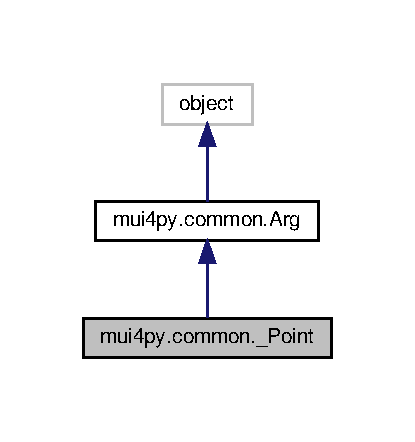
\includegraphics[width=199pt]{classmui4py_1_1common_1_1___point__inherit__graph}
\end{center}
\end{figure}


Collaboration diagram for mui4py.\+common.\+\_\+\+Point\+:
\nopagebreak
\begin{figure}[H]
\begin{center}
\leavevmode
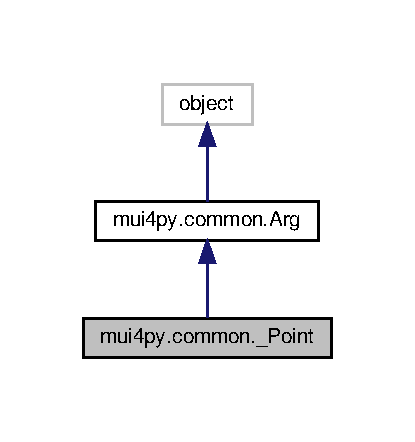
\includegraphics[width=199pt]{classmui4py_1_1common_1_1___point__coll__graph}
\end{center}
\end{figure}
\subsection*{Public Member Functions}
\begin{DoxyCompactItemize}
\item 
def \hyperlink{classmui4py_1_1common_1_1___point_a7792905e360a77e20f8b6cee900f21c0}{\+\_\+\+\_\+init\+\_\+\+\_\+} (self, \hyperlink{classmui4py_1_1common_1_1___point_a337dfb20de4ddaf91b00f97009b2f802}{point\+\_\+rep})
\item 
def \hyperlink{classmui4py_1_1common_1_1___point_af56797381e5a36d073213329cd16a757}{configure} (self, config, cpp\+\_\+point)
\end{DoxyCompactItemize}
\subsection*{Public Attributes}
\begin{DoxyCompactItemize}
\item 
\hyperlink{classmui4py_1_1common_1_1___point_a337dfb20de4ddaf91b00f97009b2f802}{point\+\_\+rep}
\item 
\hyperlink{classmui4py_1_1common_1_1___point_a4559e5eb1b5dfbcd2f364874d9708671}{arg}
\end{DoxyCompactItemize}


\subsection{Constructor \& Destructor Documentation}
\mbox{\Hypertarget{classmui4py_1_1common_1_1___point_a7792905e360a77e20f8b6cee900f21c0}\label{classmui4py_1_1common_1_1___point_a7792905e360a77e20f8b6cee900f21c0}} 
\index{mui4py\+::common\+::\+\_\+\+Point@{mui4py\+::common\+::\+\_\+\+Point}!\+\_\+\+\_\+init\+\_\+\+\_\+@{\+\_\+\+\_\+init\+\_\+\+\_\+}}
\index{\+\_\+\+\_\+init\+\_\+\+\_\+@{\+\_\+\+\_\+init\+\_\+\+\_\+}!mui4py\+::common\+::\+\_\+\+Point@{mui4py\+::common\+::\+\_\+\+Point}}
\subsubsection{\texorpdfstring{\+\_\+\+\_\+init\+\_\+\+\_\+()}{\_\_init\_\_()}}
{\footnotesize\ttfamily def mui4py.\+common.\+\_\+\+Point.\+\_\+\+\_\+init\+\_\+\+\_\+ (\begin{DoxyParamCaption}\item[{}]{self,  }\item[{}]{point\+\_\+rep }\end{DoxyParamCaption})}



\subsection{Member Function Documentation}
\mbox{\Hypertarget{classmui4py_1_1common_1_1___point_af56797381e5a36d073213329cd16a757}\label{classmui4py_1_1common_1_1___point_af56797381e5a36d073213329cd16a757}} 
\index{mui4py\+::common\+::\+\_\+\+Point@{mui4py\+::common\+::\+\_\+\+Point}!configure@{configure}}
\index{configure@{configure}!mui4py\+::common\+::\+\_\+\+Point@{mui4py\+::common\+::\+\_\+\+Point}}
\subsubsection{\texorpdfstring{configure()}{configure()}}
{\footnotesize\ttfamily def mui4py.\+common.\+\_\+\+Point.\+configure (\begin{DoxyParamCaption}\item[{}]{self,  }\item[{}]{config,  }\item[{}]{cpp\+\_\+point }\end{DoxyParamCaption})}



\subsection{Member Data Documentation}
\mbox{\Hypertarget{classmui4py_1_1common_1_1___point_a4559e5eb1b5dfbcd2f364874d9708671}\label{classmui4py_1_1common_1_1___point_a4559e5eb1b5dfbcd2f364874d9708671}} 
\index{mui4py\+::common\+::\+\_\+\+Point@{mui4py\+::common\+::\+\_\+\+Point}!arg@{arg}}
\index{arg@{arg}!mui4py\+::common\+::\+\_\+\+Point@{mui4py\+::common\+::\+\_\+\+Point}}
\subsubsection{\texorpdfstring{arg}{arg}}
{\footnotesize\ttfamily mui4py.\+common.\+\_\+\+Point.\+arg}

\mbox{\Hypertarget{classmui4py_1_1common_1_1___point_a337dfb20de4ddaf91b00f97009b2f802}\label{classmui4py_1_1common_1_1___point_a337dfb20de4ddaf91b00f97009b2f802}} 
\index{mui4py\+::common\+::\+\_\+\+Point@{mui4py\+::common\+::\+\_\+\+Point}!point\+\_\+rep@{point\+\_\+rep}}
\index{point\+\_\+rep@{point\+\_\+rep}!mui4py\+::common\+::\+\_\+\+Point@{mui4py\+::common\+::\+\_\+\+Point}}
\subsubsection{\texorpdfstring{point\+\_\+rep}{point\_rep}}
{\footnotesize\ttfamily mui4py.\+common.\+\_\+\+Point.\+point\+\_\+rep}



The documentation for this class was generated from the following file\+:\begin{DoxyCompactItemize}
\item 
wrappers/\+Python/mui4py/\hyperlink{common_8py}{common.\+py}\end{DoxyCompactItemize}

\hypertarget{classmui_1_1geometry_1_1any__shape}{}\section{mui\+:\+:geometry\+:\+:any\+\_\+shape$<$ C\+O\+N\+F\+IG $>$ Class Template Reference}
\label{classmui_1_1geometry_1_1any__shape}\index{mui\+::geometry\+::any\+\_\+shape$<$ C\+O\+N\+F\+I\+G $>$@{mui\+::geometry\+::any\+\_\+shape$<$ C\+O\+N\+F\+I\+G $>$}}


{\ttfamily \#include $<$geometry.\+h$>$}

\subsection*{Public Member Functions}
\begin{DoxyCompactItemize}
\item 
\hyperlink{classmui_1_1geometry_1_1any__shape_a63f34ab51f6745f1b004a251ecce6a44}{any\+\_\+shape} ()=default
\item 
\hyperlink{classmui_1_1geometry_1_1any__shape_a4992baf3b21a4e5ab73db0d7131d4cf7}{any\+\_\+shape} (const \hyperlink{classmui_1_1geometry_1_1any__shape}{any\+\_\+shape} \&rhs)
\item 
\hyperlink{classmui_1_1geometry_1_1any__shape_af9f12f87e8eb84b835392a6e03b3b9b0}{any\+\_\+shape} (\hyperlink{classmui_1_1geometry_1_1any__shape}{any\+\_\+shape} \&\&) noexcept=default
\item 
\hyperlink{classmui_1_1geometry_1_1any__shape_a9136caaea6ffd611d1aeced0cd9297dc}{any\+\_\+shape} (const \hyperlink{classmui_1_1geometry_1_1shape}{shape}$<$ C\+O\+N\+F\+IG $>$ \&rhs)
\item 
\hyperlink{classmui_1_1geometry_1_1any__shape}{any\+\_\+shape} \& \hyperlink{classmui_1_1geometry_1_1any__shape_aadfe3d85f7cb88e8940b6812122023b1}{operator=} (\hyperlink{classmui_1_1geometry_1_1any__shape}{any\+\_\+shape} rhs)
\item 
\hyperlink{classmui_1_1geometry_1_1any__shape_ac8ca4985eeda1228a465a8ee0eef743f}{operator bool} () const noexcept
\item 
bool \hyperlink{classmui_1_1geometry_1_1any__shape_a1de14e805b4b17bff9ac9456591266b4}{empty} () const noexcept
\item 
void \hyperlink{classmui_1_1geometry_1_1any__shape_a872a9094ca9513b0aa93c1a1fe5c719a}{swap} (\hyperlink{classmui_1_1geometry_1_1any__shape}{any\+\_\+shape} \&rhs) noexcept
\item 
\hyperlink{classmui_1_1geometry_1_1shape}{shape}$<$ C\+O\+N\+F\+IG $>$ \& \hyperlink{classmui_1_1geometry_1_1any__shape_a9dcdce6998e255afc8258e3d0c867577}{get} ()
\item 
const \hyperlink{classmui_1_1geometry_1_1shape}{shape}$<$ C\+O\+N\+F\+IG $>$ \& \hyperlink{classmui_1_1geometry_1_1any__shape_a9ba06a270236bd9a25207f429b869303}{get} () const
\item 
\hyperlink{namespacemui_1_1geometry_a5f311a343181e2f20482e5c9afb0f136}{shape\+\_\+type} \hyperlink{classmui_1_1geometry_1_1any__shape_adcce217426f80b4a1a17c3659764b607}{type} () const noexcept
\item 
\hyperlink{classmui_1_1geometry_1_1box}{box}$<$ C\+O\+N\+F\+IG $>$ \hyperlink{classmui_1_1geometry_1_1any__shape_ad05e91914ca393723f5651cf57c99775}{bbox} () const
\end{DoxyCompactItemize}
\subsection*{Friends}
\begin{DoxyCompactItemize}
\item 
\hyperlink{classmui_1_1ostream}{ostream} \& \hyperlink{classmui_1_1geometry_1_1any__shape_a3e1a091d6ee6e70e3bd7f3c3e7ae2735}{operator$<$$<$} (\hyperlink{classmui_1_1ostream}{ostream} \&stream, const \hyperlink{classmui_1_1geometry_1_1any__shape}{any\+\_\+shape} \&obj)
\item 
\hyperlink{classmui_1_1istream}{istream} \& \hyperlink{classmui_1_1geometry_1_1any__shape_ab8882ff239d9c3dde4576f36f949e500}{operator$>$$>$} (\hyperlink{classmui_1_1istream}{istream} \&stream, \hyperlink{classmui_1_1geometry_1_1any__shape}{any\+\_\+shape} \&obj)
\end{DoxyCompactItemize}


\subsection{Constructor \& Destructor Documentation}
\mbox{\Hypertarget{classmui_1_1geometry_1_1any__shape_a63f34ab51f6745f1b004a251ecce6a44}\label{classmui_1_1geometry_1_1any__shape_a63f34ab51f6745f1b004a251ecce6a44}} 
\index{mui\+::geometry\+::any\+\_\+shape@{mui\+::geometry\+::any\+\_\+shape}!any\+\_\+shape@{any\+\_\+shape}}
\index{any\+\_\+shape@{any\+\_\+shape}!mui\+::geometry\+::any\+\_\+shape@{mui\+::geometry\+::any\+\_\+shape}}
\subsubsection{\texorpdfstring{any\+\_\+shape()}{any\_shape()}\hspace{0.1cm}{\footnotesize\ttfamily [1/4]}}
{\footnotesize\ttfamily template$<$typename C\+O\+N\+F\+IG$>$ \\
\hyperlink{classmui_1_1geometry_1_1any__shape}{mui\+::geometry\+::any\+\_\+shape}$<$ C\+O\+N\+F\+IG $>$\+::\hyperlink{classmui_1_1geometry_1_1any__shape}{any\+\_\+shape} (\begin{DoxyParamCaption}{ }\end{DoxyParamCaption})\hspace{0.3cm}{\ttfamily [default]}}

\mbox{\Hypertarget{classmui_1_1geometry_1_1any__shape_a4992baf3b21a4e5ab73db0d7131d4cf7}\label{classmui_1_1geometry_1_1any__shape_a4992baf3b21a4e5ab73db0d7131d4cf7}} 
\index{mui\+::geometry\+::any\+\_\+shape@{mui\+::geometry\+::any\+\_\+shape}!any\+\_\+shape@{any\+\_\+shape}}
\index{any\+\_\+shape@{any\+\_\+shape}!mui\+::geometry\+::any\+\_\+shape@{mui\+::geometry\+::any\+\_\+shape}}
\subsubsection{\texorpdfstring{any\+\_\+shape()}{any\_shape()}\hspace{0.1cm}{\footnotesize\ttfamily [2/4]}}
{\footnotesize\ttfamily template$<$typename C\+O\+N\+F\+IG$>$ \\
\hyperlink{classmui_1_1geometry_1_1any__shape}{mui\+::geometry\+::any\+\_\+shape}$<$ C\+O\+N\+F\+IG $>$\+::\hyperlink{classmui_1_1geometry_1_1any__shape}{any\+\_\+shape} (\begin{DoxyParamCaption}\item[{const \hyperlink{classmui_1_1geometry_1_1any__shape}{any\+\_\+shape}$<$ C\+O\+N\+F\+IG $>$ \&}]{rhs }\end{DoxyParamCaption})\hspace{0.3cm}{\ttfamily [inline]}}

\mbox{\Hypertarget{classmui_1_1geometry_1_1any__shape_af9f12f87e8eb84b835392a6e03b3b9b0}\label{classmui_1_1geometry_1_1any__shape_af9f12f87e8eb84b835392a6e03b3b9b0}} 
\index{mui\+::geometry\+::any\+\_\+shape@{mui\+::geometry\+::any\+\_\+shape}!any\+\_\+shape@{any\+\_\+shape}}
\index{any\+\_\+shape@{any\+\_\+shape}!mui\+::geometry\+::any\+\_\+shape@{mui\+::geometry\+::any\+\_\+shape}}
\subsubsection{\texorpdfstring{any\+\_\+shape()}{any\_shape()}\hspace{0.1cm}{\footnotesize\ttfamily [3/4]}}
{\footnotesize\ttfamily template$<$typename C\+O\+N\+F\+IG$>$ \\
\hyperlink{classmui_1_1geometry_1_1any__shape}{mui\+::geometry\+::any\+\_\+shape}$<$ C\+O\+N\+F\+IG $>$\+::\hyperlink{classmui_1_1geometry_1_1any__shape}{any\+\_\+shape} (\begin{DoxyParamCaption}\item[{\hyperlink{classmui_1_1geometry_1_1any__shape}{any\+\_\+shape}$<$ C\+O\+N\+F\+IG $>$ \&\&}]{ }\end{DoxyParamCaption})\hspace{0.3cm}{\ttfamily [default]}, {\ttfamily [noexcept]}}

\mbox{\Hypertarget{classmui_1_1geometry_1_1any__shape_a9136caaea6ffd611d1aeced0cd9297dc}\label{classmui_1_1geometry_1_1any__shape_a9136caaea6ffd611d1aeced0cd9297dc}} 
\index{mui\+::geometry\+::any\+\_\+shape@{mui\+::geometry\+::any\+\_\+shape}!any\+\_\+shape@{any\+\_\+shape}}
\index{any\+\_\+shape@{any\+\_\+shape}!mui\+::geometry\+::any\+\_\+shape@{mui\+::geometry\+::any\+\_\+shape}}
\subsubsection{\texorpdfstring{any\+\_\+shape()}{any\_shape()}\hspace{0.1cm}{\footnotesize\ttfamily [4/4]}}
{\footnotesize\ttfamily template$<$typename C\+O\+N\+F\+IG$>$ \\
\hyperlink{classmui_1_1geometry_1_1any__shape}{mui\+::geometry\+::any\+\_\+shape}$<$ C\+O\+N\+F\+IG $>$\+::\hyperlink{classmui_1_1geometry_1_1any__shape}{any\+\_\+shape} (\begin{DoxyParamCaption}\item[{const \hyperlink{classmui_1_1geometry_1_1shape}{shape}$<$ C\+O\+N\+F\+IG $>$ \&}]{rhs }\end{DoxyParamCaption})\hspace{0.3cm}{\ttfamily [inline]}}



\subsection{Member Function Documentation}
\mbox{\Hypertarget{classmui_1_1geometry_1_1any__shape_ad05e91914ca393723f5651cf57c99775}\label{classmui_1_1geometry_1_1any__shape_ad05e91914ca393723f5651cf57c99775}} 
\index{mui\+::geometry\+::any\+\_\+shape@{mui\+::geometry\+::any\+\_\+shape}!bbox@{bbox}}
\index{bbox@{bbox}!mui\+::geometry\+::any\+\_\+shape@{mui\+::geometry\+::any\+\_\+shape}}
\subsubsection{\texorpdfstring{bbox()}{bbox()}}
{\footnotesize\ttfamily template$<$typename C\+O\+N\+F\+IG $>$ \\
\hyperlink{classmui_1_1geometry_1_1box}{box}$<$ C\+O\+N\+F\+IG $>$ \hyperlink{classmui_1_1geometry_1_1any__shape}{mui\+::geometry\+::any\+\_\+shape}$<$ C\+O\+N\+F\+IG $>$\+::bbox (\begin{DoxyParamCaption}{ }\end{DoxyParamCaption}) const}

\mbox{\Hypertarget{classmui_1_1geometry_1_1any__shape_a1de14e805b4b17bff9ac9456591266b4}\label{classmui_1_1geometry_1_1any__shape_a1de14e805b4b17bff9ac9456591266b4}} 
\index{mui\+::geometry\+::any\+\_\+shape@{mui\+::geometry\+::any\+\_\+shape}!empty@{empty}}
\index{empty@{empty}!mui\+::geometry\+::any\+\_\+shape@{mui\+::geometry\+::any\+\_\+shape}}
\subsubsection{\texorpdfstring{empty()}{empty()}}
{\footnotesize\ttfamily template$<$typename C\+O\+N\+F\+IG$>$ \\
bool \hyperlink{classmui_1_1geometry_1_1any__shape}{mui\+::geometry\+::any\+\_\+shape}$<$ C\+O\+N\+F\+IG $>$\+::empty (\begin{DoxyParamCaption}{ }\end{DoxyParamCaption}) const\hspace{0.3cm}{\ttfamily [inline]}, {\ttfamily [noexcept]}}

\mbox{\Hypertarget{classmui_1_1geometry_1_1any__shape_a9dcdce6998e255afc8258e3d0c867577}\label{classmui_1_1geometry_1_1any__shape_a9dcdce6998e255afc8258e3d0c867577}} 
\index{mui\+::geometry\+::any\+\_\+shape@{mui\+::geometry\+::any\+\_\+shape}!get@{get}}
\index{get@{get}!mui\+::geometry\+::any\+\_\+shape@{mui\+::geometry\+::any\+\_\+shape}}
\subsubsection{\texorpdfstring{get()}{get()}\hspace{0.1cm}{\footnotesize\ttfamily [1/2]}}
{\footnotesize\ttfamily template$<$typename C\+O\+N\+F\+IG$>$ \\
\hyperlink{classmui_1_1geometry_1_1shape}{shape}$<$C\+O\+N\+F\+IG$>$\& \hyperlink{classmui_1_1geometry_1_1any__shape}{mui\+::geometry\+::any\+\_\+shape}$<$ C\+O\+N\+F\+IG $>$\+::get (\begin{DoxyParamCaption}{ }\end{DoxyParamCaption})\hspace{0.3cm}{\ttfamily [inline]}}

\mbox{\Hypertarget{classmui_1_1geometry_1_1any__shape_a9ba06a270236bd9a25207f429b869303}\label{classmui_1_1geometry_1_1any__shape_a9ba06a270236bd9a25207f429b869303}} 
\index{mui\+::geometry\+::any\+\_\+shape@{mui\+::geometry\+::any\+\_\+shape}!get@{get}}
\index{get@{get}!mui\+::geometry\+::any\+\_\+shape@{mui\+::geometry\+::any\+\_\+shape}}
\subsubsection{\texorpdfstring{get()}{get()}\hspace{0.1cm}{\footnotesize\ttfamily [2/2]}}
{\footnotesize\ttfamily template$<$typename C\+O\+N\+F\+IG$>$ \\
const \hyperlink{classmui_1_1geometry_1_1shape}{shape}$<$C\+O\+N\+F\+IG$>$\& \hyperlink{classmui_1_1geometry_1_1any__shape}{mui\+::geometry\+::any\+\_\+shape}$<$ C\+O\+N\+F\+IG $>$\+::get (\begin{DoxyParamCaption}{ }\end{DoxyParamCaption}) const\hspace{0.3cm}{\ttfamily [inline]}}

\mbox{\Hypertarget{classmui_1_1geometry_1_1any__shape_ac8ca4985eeda1228a465a8ee0eef743f}\label{classmui_1_1geometry_1_1any__shape_ac8ca4985eeda1228a465a8ee0eef743f}} 
\index{mui\+::geometry\+::any\+\_\+shape@{mui\+::geometry\+::any\+\_\+shape}!operator bool@{operator bool}}
\index{operator bool@{operator bool}!mui\+::geometry\+::any\+\_\+shape@{mui\+::geometry\+::any\+\_\+shape}}
\subsubsection{\texorpdfstring{operator bool()}{operator bool()}}
{\footnotesize\ttfamily template$<$typename C\+O\+N\+F\+IG$>$ \\
\hyperlink{classmui_1_1geometry_1_1any__shape}{mui\+::geometry\+::any\+\_\+shape}$<$ C\+O\+N\+F\+IG $>$\+::operator bool (\begin{DoxyParamCaption}{ }\end{DoxyParamCaption}) const\hspace{0.3cm}{\ttfamily [inline]}, {\ttfamily [explicit]}, {\ttfamily [noexcept]}}

\mbox{\Hypertarget{classmui_1_1geometry_1_1any__shape_aadfe3d85f7cb88e8940b6812122023b1}\label{classmui_1_1geometry_1_1any__shape_aadfe3d85f7cb88e8940b6812122023b1}} 
\index{mui\+::geometry\+::any\+\_\+shape@{mui\+::geometry\+::any\+\_\+shape}!operator=@{operator=}}
\index{operator=@{operator=}!mui\+::geometry\+::any\+\_\+shape@{mui\+::geometry\+::any\+\_\+shape}}
\subsubsection{\texorpdfstring{operator=()}{operator=()}}
{\footnotesize\ttfamily template$<$typename C\+O\+N\+F\+IG$>$ \\
\hyperlink{classmui_1_1geometry_1_1any__shape}{any\+\_\+shape}\& \hyperlink{classmui_1_1geometry_1_1any__shape}{mui\+::geometry\+::any\+\_\+shape}$<$ C\+O\+N\+F\+IG $>$\+::operator= (\begin{DoxyParamCaption}\item[{\hyperlink{classmui_1_1geometry_1_1any__shape}{any\+\_\+shape}$<$ C\+O\+N\+F\+IG $>$}]{rhs }\end{DoxyParamCaption})\hspace{0.3cm}{\ttfamily [inline]}}

\mbox{\Hypertarget{classmui_1_1geometry_1_1any__shape_a872a9094ca9513b0aa93c1a1fe5c719a}\label{classmui_1_1geometry_1_1any__shape_a872a9094ca9513b0aa93c1a1fe5c719a}} 
\index{mui\+::geometry\+::any\+\_\+shape@{mui\+::geometry\+::any\+\_\+shape}!swap@{swap}}
\index{swap@{swap}!mui\+::geometry\+::any\+\_\+shape@{mui\+::geometry\+::any\+\_\+shape}}
\subsubsection{\texorpdfstring{swap()}{swap()}}
{\footnotesize\ttfamily template$<$typename C\+O\+N\+F\+IG$>$ \\
void \hyperlink{classmui_1_1geometry_1_1any__shape}{mui\+::geometry\+::any\+\_\+shape}$<$ C\+O\+N\+F\+IG $>$\+::swap (\begin{DoxyParamCaption}\item[{\hyperlink{classmui_1_1geometry_1_1any__shape}{any\+\_\+shape}$<$ C\+O\+N\+F\+IG $>$ \&}]{rhs }\end{DoxyParamCaption})\hspace{0.3cm}{\ttfamily [inline]}, {\ttfamily [noexcept]}}

\mbox{\Hypertarget{classmui_1_1geometry_1_1any__shape_adcce217426f80b4a1a17c3659764b607}\label{classmui_1_1geometry_1_1any__shape_adcce217426f80b4a1a17c3659764b607}} 
\index{mui\+::geometry\+::any\+\_\+shape@{mui\+::geometry\+::any\+\_\+shape}!type@{type}}
\index{type@{type}!mui\+::geometry\+::any\+\_\+shape@{mui\+::geometry\+::any\+\_\+shape}}
\subsubsection{\texorpdfstring{type()}{type()}}
{\footnotesize\ttfamily template$<$typename C\+O\+N\+F\+IG$>$ \\
\hyperlink{namespacemui_1_1geometry_a5f311a343181e2f20482e5c9afb0f136}{shape\+\_\+type} \hyperlink{classmui_1_1geometry_1_1any__shape}{mui\+::geometry\+::any\+\_\+shape}$<$ C\+O\+N\+F\+IG $>$\+::type (\begin{DoxyParamCaption}{ }\end{DoxyParamCaption}) const\hspace{0.3cm}{\ttfamily [inline]}, {\ttfamily [noexcept]}}



\subsection{Friends And Related Function Documentation}
\mbox{\Hypertarget{classmui_1_1geometry_1_1any__shape_a3e1a091d6ee6e70e3bd7f3c3e7ae2735}\label{classmui_1_1geometry_1_1any__shape_a3e1a091d6ee6e70e3bd7f3c3e7ae2735}} 
\index{mui\+::geometry\+::any\+\_\+shape@{mui\+::geometry\+::any\+\_\+shape}!operator$<$$<$@{operator$<$$<$}}
\index{operator$<$$<$@{operator$<$$<$}!mui\+::geometry\+::any\+\_\+shape@{mui\+::geometry\+::any\+\_\+shape}}
\subsubsection{\texorpdfstring{operator$<$$<$}{operator<<}}
{\footnotesize\ttfamily template$<$typename C\+O\+N\+F\+IG$>$ \\
\hyperlink{classmui_1_1ostream}{ostream}\& operator$<$$<$ (\begin{DoxyParamCaption}\item[{\hyperlink{classmui_1_1ostream}{ostream} \&}]{stream,  }\item[{const \hyperlink{classmui_1_1geometry_1_1any__shape}{any\+\_\+shape}$<$ C\+O\+N\+F\+IG $>$ \&}]{obj }\end{DoxyParamCaption})\hspace{0.3cm}{\ttfamily [friend]}}

\mbox{\Hypertarget{classmui_1_1geometry_1_1any__shape_ab8882ff239d9c3dde4576f36f949e500}\label{classmui_1_1geometry_1_1any__shape_ab8882ff239d9c3dde4576f36f949e500}} 
\index{mui\+::geometry\+::any\+\_\+shape@{mui\+::geometry\+::any\+\_\+shape}!operator$>$$>$@{operator$>$$>$}}
\index{operator$>$$>$@{operator$>$$>$}!mui\+::geometry\+::any\+\_\+shape@{mui\+::geometry\+::any\+\_\+shape}}
\subsubsection{\texorpdfstring{operator$>$$>$}{operator>>}}
{\footnotesize\ttfamily template$<$typename C\+O\+N\+F\+IG$>$ \\
\hyperlink{classmui_1_1istream}{istream}\& operator$>$$>$ (\begin{DoxyParamCaption}\item[{\hyperlink{classmui_1_1istream}{istream} \&}]{stream,  }\item[{\hyperlink{classmui_1_1geometry_1_1any__shape}{any\+\_\+shape}$<$ C\+O\+N\+F\+IG $>$ \&}]{obj }\end{DoxyParamCaption})\hspace{0.3cm}{\ttfamily [friend]}}



The documentation for this class was generated from the following file\+:\begin{DoxyCompactItemize}
\item 
\hyperlink{geometry_8h}{geometry.\+h}\end{DoxyCompactItemize}

\hypertarget{classmui4py_1_1common_1_1_arg}{}\section{mui4py.\+common.\+Arg Class Reference}
\label{classmui4py_1_1common_1_1_arg}\index{mui4py.\+common.\+Arg@{mui4py.\+common.\+Arg}}


Inheritance diagram for mui4py.\+common.\+Arg\+:
\nopagebreak
\begin{figure}[H]
\begin{center}
\leavevmode
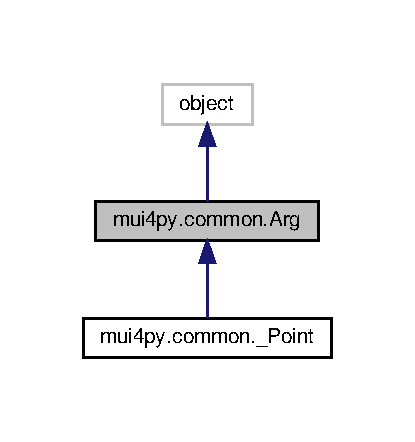
\includegraphics[width=199pt]{classmui4py_1_1common_1_1_arg__inherit__graph}
\end{center}
\end{figure}


Collaboration diagram for mui4py.\+common.\+Arg\+:
\nopagebreak
\begin{figure}[H]
\begin{center}
\leavevmode
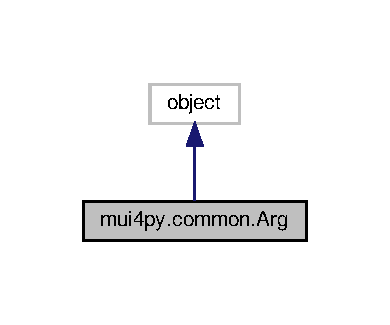
\includegraphics[width=187pt]{classmui4py_1_1common_1_1_arg__coll__graph}
\end{center}
\end{figure}
\subsection*{Public Member Functions}
\begin{DoxyCompactItemize}
\item 
def \hyperlink{classmui4py_1_1common_1_1_arg_a2eaf791d82b8a8663316ede9133432d5}{\+\_\+\+\_\+init\+\_\+\+\_\+} (self, \hyperlink{classmui4py_1_1common_1_1_arg_a45ebd7fb8f9080eb469557f4e77e6f0c}{arg})
\item 
def \hyperlink{classmui4py_1_1common_1_1_arg_a045ba65aadaa1d6f9c5dd669dd9fef81}{configure} (self, config, cpp\+\_\+point)
\end{DoxyCompactItemize}
\subsection*{Public Attributes}
\begin{DoxyCompactItemize}
\item 
\hyperlink{classmui4py_1_1common_1_1_arg_a45ebd7fb8f9080eb469557f4e77e6f0c}{arg}
\end{DoxyCompactItemize}


\subsection{Constructor \& Destructor Documentation}
\mbox{\Hypertarget{classmui4py_1_1common_1_1_arg_a2eaf791d82b8a8663316ede9133432d5}\label{classmui4py_1_1common_1_1_arg_a2eaf791d82b8a8663316ede9133432d5}} 
\index{mui4py\+::common\+::\+Arg@{mui4py\+::common\+::\+Arg}!\+\_\+\+\_\+init\+\_\+\+\_\+@{\+\_\+\+\_\+init\+\_\+\+\_\+}}
\index{\+\_\+\+\_\+init\+\_\+\+\_\+@{\+\_\+\+\_\+init\+\_\+\+\_\+}!mui4py\+::common\+::\+Arg@{mui4py\+::common\+::\+Arg}}
\subsubsection{\texorpdfstring{\+\_\+\+\_\+init\+\_\+\+\_\+()}{\_\_init\_\_()}}
{\footnotesize\ttfamily def mui4py.\+common.\+Arg.\+\_\+\+\_\+init\+\_\+\+\_\+ (\begin{DoxyParamCaption}\item[{}]{self,  }\item[{}]{arg }\end{DoxyParamCaption})}



\subsection{Member Function Documentation}
\mbox{\Hypertarget{classmui4py_1_1common_1_1_arg_a045ba65aadaa1d6f9c5dd669dd9fef81}\label{classmui4py_1_1common_1_1_arg_a045ba65aadaa1d6f9c5dd669dd9fef81}} 
\index{mui4py\+::common\+::\+Arg@{mui4py\+::common\+::\+Arg}!configure@{configure}}
\index{configure@{configure}!mui4py\+::common\+::\+Arg@{mui4py\+::common\+::\+Arg}}
\subsubsection{\texorpdfstring{configure()}{configure()}}
{\footnotesize\ttfamily def mui4py.\+common.\+Arg.\+configure (\begin{DoxyParamCaption}\item[{}]{self,  }\item[{}]{config,  }\item[{}]{cpp\+\_\+point }\end{DoxyParamCaption})}



\subsection{Member Data Documentation}
\mbox{\Hypertarget{classmui4py_1_1common_1_1_arg_a45ebd7fb8f9080eb469557f4e77e6f0c}\label{classmui4py_1_1common_1_1_arg_a45ebd7fb8f9080eb469557f4e77e6f0c}} 
\index{mui4py\+::common\+::\+Arg@{mui4py\+::common\+::\+Arg}!arg@{arg}}
\index{arg@{arg}!mui4py\+::common\+::\+Arg@{mui4py\+::common\+::\+Arg}}
\subsubsection{\texorpdfstring{arg}{arg}}
{\footnotesize\ttfamily mui4py.\+common.\+Arg.\+arg}



The documentation for this class was generated from the following file\+:\begin{DoxyCompactItemize}
\item 
wrappers/\+Python/mui4py/\hyperlink{common_8py}{common.\+py}\end{DoxyCompactItemize}

\hypertarget{structmui_1_1bad__storage__cast}{}\section{mui\+:\+:bad\+\_\+storage\+\_\+cast Struct Reference}
\label{structmui_1_1bad__storage__cast}\index{mui\+::bad\+\_\+storage\+\_\+cast@{mui\+::bad\+\_\+storage\+\_\+cast}}


{\ttfamily \#include $<$dynstorage.\+h$>$}



Inheritance diagram for mui\+:\+:bad\+\_\+storage\+\_\+cast\+:
\nopagebreak
\begin{figure}[H]
\begin{center}
\leavevmode
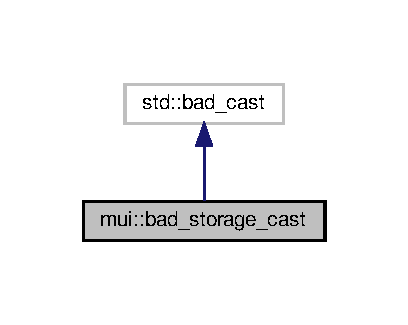
\includegraphics[width=196pt]{structmui_1_1bad__storage__cast__inherit__graph}
\end{center}
\end{figure}


Collaboration diagram for mui\+:\+:bad\+\_\+storage\+\_\+cast\+:
\nopagebreak
\begin{figure}[H]
\begin{center}
\leavevmode
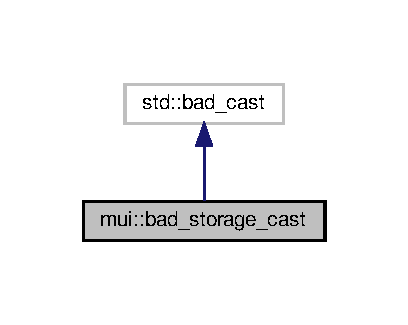
\includegraphics[width=196pt]{structmui_1_1bad__storage__cast__coll__graph}
\end{center}
\end{figure}
\subsection*{Public Member Functions}
\begin{DoxyCompactItemize}
\item 
virtual const char $\ast$ \hyperlink{structmui_1_1bad__storage__cast_a052cbf41469ca194b4f423ea523f0071}{what} () const noexcept
\end{DoxyCompactItemize}


\subsection{Member Function Documentation}
\mbox{\Hypertarget{structmui_1_1bad__storage__cast_a052cbf41469ca194b4f423ea523f0071}\label{structmui_1_1bad__storage__cast_a052cbf41469ca194b4f423ea523f0071}} 
\index{mui\+::bad\+\_\+storage\+\_\+cast@{mui\+::bad\+\_\+storage\+\_\+cast}!what@{what}}
\index{what@{what}!mui\+::bad\+\_\+storage\+\_\+cast@{mui\+::bad\+\_\+storage\+\_\+cast}}
\subsubsection{\texorpdfstring{what()}{what()}}
{\footnotesize\ttfamily virtual const char$\ast$ mui\+::bad\+\_\+storage\+\_\+cast\+::what (\begin{DoxyParamCaption}{ }\end{DoxyParamCaption}) const\hspace{0.3cm}{\ttfamily [inline]}, {\ttfamily [virtual]}, {\ttfamily [noexcept]}}



The documentation for this struct was generated from the following file\+:\begin{DoxyCompactItemize}
\item 
\hyperlink{dynstorage_8h}{dynstorage.\+h}\end{DoxyCompactItemize}

\hypertarget{structmui_1_1bad__storage__id}{}\section{mui\+:\+:bad\+\_\+storage\+\_\+id Struct Reference}
\label{structmui_1_1bad__storage__id}\index{mui\+::bad\+\_\+storage\+\_\+id@{mui\+::bad\+\_\+storage\+\_\+id}}


{\ttfamily \#include $<$dynstorage.\+h$>$}



Inheritance diagram for mui\+:\+:bad\+\_\+storage\+\_\+id\+:
\nopagebreak
\begin{figure}[H]
\begin{center}
\leavevmode
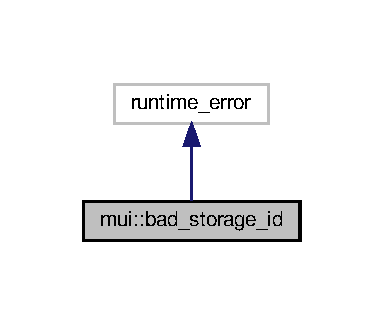
\includegraphics[width=184pt]{structmui_1_1bad__storage__id__inherit__graph}
\end{center}
\end{figure}


Collaboration diagram for mui\+:\+:bad\+\_\+storage\+\_\+id\+:
\nopagebreak
\begin{figure}[H]
\begin{center}
\leavevmode
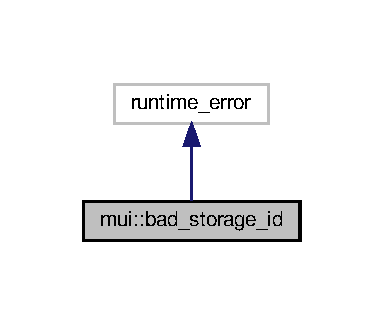
\includegraphics[width=184pt]{structmui_1_1bad__storage__id__coll__graph}
\end{center}
\end{figure}
\subsection*{Public Member Functions}
\begin{DoxyCompactItemize}
\item 
\hyperlink{structmui_1_1bad__storage__id_a5daf39721cbd9687cf9351d609386f9c}{bad\+\_\+storage\+\_\+id} (const char $\ast$err)
\end{DoxyCompactItemize}


\subsection{Constructor \& Destructor Documentation}
\mbox{\Hypertarget{structmui_1_1bad__storage__id_a5daf39721cbd9687cf9351d609386f9c}\label{structmui_1_1bad__storage__id_a5daf39721cbd9687cf9351d609386f9c}} 
\index{mui\+::bad\+\_\+storage\+\_\+id@{mui\+::bad\+\_\+storage\+\_\+id}!bad\+\_\+storage\+\_\+id@{bad\+\_\+storage\+\_\+id}}
\index{bad\+\_\+storage\+\_\+id@{bad\+\_\+storage\+\_\+id}!mui\+::bad\+\_\+storage\+\_\+id@{mui\+::bad\+\_\+storage\+\_\+id}}
\subsubsection{\texorpdfstring{bad\+\_\+storage\+\_\+id()}{bad\_storage\_id()}}
{\footnotesize\ttfamily mui\+::bad\+\_\+storage\+\_\+id\+::bad\+\_\+storage\+\_\+id (\begin{DoxyParamCaption}\item[{const char $\ast$}]{err }\end{DoxyParamCaption})\hspace{0.3cm}{\ttfamily [inline]}}



The documentation for this struct was generated from the following file\+:\begin{DoxyCompactItemize}
\item 
\hyperlink{dynstorage_8h}{dynstorage.\+h}\end{DoxyCompactItemize}

\hypertarget{structmui_1_1bin__iterator}{}\section{mui\+:\+:bin\+\_\+iterator$<$ T, C\+O\+N\+F\+IG $>$ Struct Template Reference}
\label{structmui_1_1bin__iterator}\index{mui\+::bin\+\_\+iterator$<$ T, C\+O\+N\+F\+I\+G $>$@{mui\+::bin\+\_\+iterator$<$ T, C\+O\+N\+F\+I\+G $>$}}


{\ttfamily \#include $<$bin.\+h$>$}



Inheritance diagram for mui\+:\+:bin\+\_\+iterator$<$ T, C\+O\+N\+F\+IG $>$\+:
\nopagebreak
\begin{figure}[H]
\begin{center}
\leavevmode
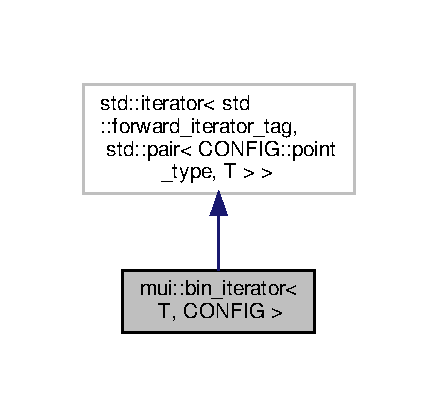
\includegraphics[width=210pt]{structmui_1_1bin__iterator__inherit__graph}
\end{center}
\end{figure}


Collaboration diagram for mui\+:\+:bin\+\_\+iterator$<$ T, C\+O\+N\+F\+IG $>$\+:
\nopagebreak
\begin{figure}[H]
\begin{center}
\leavevmode
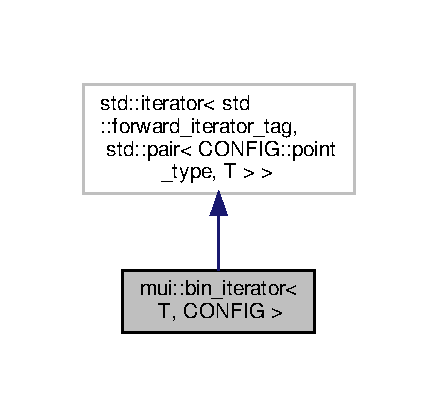
\includegraphics[width=210pt]{structmui_1_1bin__iterator__coll__graph}
\end{center}
\end{figure}
\subsection*{Public Types}
\begin{DoxyCompactItemize}
\item 
using \hyperlink{structmui_1_1bin__iterator_a647b888410c7aec82b750400f5d5c283}{P} = std\+::pair$<$ typename C\+O\+N\+F\+I\+G\+::point\+\_\+type, T $>$
\end{DoxyCompactItemize}
\subsection*{Public Member Functions}
\begin{DoxyCompactItemize}
\item 
\hyperlink{structmui_1_1bin__iterator_ad4a934e39ea52abb9b9df227826e784b}{bin\+\_\+iterator} (const \hyperlink{structmui_1_1bin__range}{bin\+\_\+range}$<$ T, C\+O\+N\+F\+IG $>$ \&range\+\_\+)
\item 
\hyperlink{structmui_1_1bin__iterator_a28e68216dd247d68b9c60f99c13631c5}{bin\+\_\+iterator} (const \hyperlink{structmui_1_1bin__range}{bin\+\_\+range}$<$ T, C\+O\+N\+F\+IG $>$ \&range\+\_\+, int)
\item 
\hyperlink{structmui_1_1bin__iterator_afb02d18499dea2d212b2d220f69ce749}{bin\+\_\+iterator} (const \hyperlink{structmui_1_1bin__iterator}{bin\+\_\+iterator} \&)=default
\item 
\hyperlink{structmui_1_1bin__iterator}{bin\+\_\+iterator} \& \hyperlink{structmui_1_1bin__iterator_a4d77cf5d472236ac4d8a35bb97d70011}{operator=} (const \hyperlink{structmui_1_1bin__iterator}{bin\+\_\+iterator} \&)=default
\item 
\hyperlink{structmui_1_1bin__iterator}{bin\+\_\+iterator} \& \hyperlink{structmui_1_1bin__iterator_abcbb2de1b131606af75b303f2d8e90e9}{operator++} ()
\item 
\hyperlink{structmui_1_1bin__iterator}{bin\+\_\+iterator} \hyperlink{structmui_1_1bin__iterator_a348e1d15c037b9e1302f16dc065928fb}{operator++} (int)
\item 
void \hyperlink{structmui_1_1bin__iterator_a9dd12ec01e52a6aac8a2aa511b4a0849}{invalidate} ()
\item 
void \hyperlink{structmui_1_1bin__iterator_add20c0285e60fb2bd9e7b82bb9fb4204}{validate} ()
\item 
bool \hyperlink{structmui_1_1bin__iterator_abb2f0a6ce3579fa7f33409da0b295ea1}{operator!=} (const \hyperlink{structmui_1_1bin__iterator}{bin\+\_\+iterator} \&rhs) const
\item 
bool \hyperlink{structmui_1_1bin__iterator_a12ed131569425fd91bd853eef3dd45ef}{operator==} (const \hyperlink{structmui_1_1bin__iterator}{bin\+\_\+iterator} \&rhs) const
\item 
const \hyperlink{structmui_1_1bin__iterator_a647b888410c7aec82b750400f5d5c283}{P} \& \hyperlink{structmui_1_1bin__iterator_a03e75c57f1b080531ea1da1ad7dc8039}{operator$\ast$} () const
\item 
const \hyperlink{structmui_1_1bin__iterator_a647b888410c7aec82b750400f5d5c283}{P} $\ast$ \hyperlink{structmui_1_1bin__iterator_a4bf91868a5ca5e0cca146a11ad1ac24b}{operator-\/$>$} () const
\end{DoxyCompactItemize}
\subsection*{Public Attributes}
\begin{DoxyCompactItemize}
\item 
const \hyperlink{structmui_1_1bin__range}{bin\+\_\+range}$<$ T, C\+O\+N\+F\+IG $>$ \& \hyperlink{structmui_1_1bin__iterator_a371e739fe4b63c447a787572eb8ed055}{range}
\item 
int \hyperlink{structmui_1_1bin__iterator_a97ebdd9e81da980a9a455eef380ebf6f}{count} \mbox{[}\hyperlink{structmui_1_1bin__iterator_acb6d849efa422c9c07a5866c3031a3f8}{D}-\/1\mbox{]}
\item 
std\+::size\+\_\+t \hyperlink{structmui_1_1bin__iterator_ac6914757b751e94ba6763d82faabbc2c}{high}
\item 
std\+::size\+\_\+t \hyperlink{structmui_1_1bin__iterator_a78c714939432311507baacc85de506e4}{index}
\end{DoxyCompactItemize}
\subsection*{Static Public Attributes}
\begin{DoxyCompactItemize}
\item 
static const int \hyperlink{structmui_1_1bin__iterator_acb6d849efa422c9c07a5866c3031a3f8}{D} = C\+O\+N\+F\+I\+G\+::D
\end{DoxyCompactItemize}


\subsection{Member Typedef Documentation}
\mbox{\Hypertarget{structmui_1_1bin__iterator_a647b888410c7aec82b750400f5d5c283}\label{structmui_1_1bin__iterator_a647b888410c7aec82b750400f5d5c283}} 
\index{mui\+::bin\+\_\+iterator@{mui\+::bin\+\_\+iterator}!P@{P}}
\index{P@{P}!mui\+::bin\+\_\+iterator@{mui\+::bin\+\_\+iterator}}
\subsubsection{\texorpdfstring{P}{P}}
{\footnotesize\ttfamily template$<$typename T, typename C\+O\+N\+F\+IG$>$ \\
using \hyperlink{structmui_1_1bin__iterator}{mui\+::bin\+\_\+iterator}$<$ T, C\+O\+N\+F\+IG $>$\+::\hyperlink{structmui_1_1bin__iterator_a647b888410c7aec82b750400f5d5c283}{P} =  std\+::pair$<$typename C\+O\+N\+F\+I\+G\+::point\+\_\+type,T$>$}



\subsection{Constructor \& Destructor Documentation}
\mbox{\Hypertarget{structmui_1_1bin__iterator_ad4a934e39ea52abb9b9df227826e784b}\label{structmui_1_1bin__iterator_ad4a934e39ea52abb9b9df227826e784b}} 
\index{mui\+::bin\+\_\+iterator@{mui\+::bin\+\_\+iterator}!bin\+\_\+iterator@{bin\+\_\+iterator}}
\index{bin\+\_\+iterator@{bin\+\_\+iterator}!mui\+::bin\+\_\+iterator@{mui\+::bin\+\_\+iterator}}
\subsubsection{\texorpdfstring{bin\+\_\+iterator()}{bin\_iterator()}\hspace{0.1cm}{\footnotesize\ttfamily [1/3]}}
{\footnotesize\ttfamily template$<$typename T , typename C\+O\+N\+F\+IG $>$ \\
\hyperlink{structmui_1_1bin__iterator}{mui\+::bin\+\_\+iterator}$<$ T, C\+O\+N\+F\+IG $>$\+::\hyperlink{structmui_1_1bin__iterator}{bin\+\_\+iterator} (\begin{DoxyParamCaption}\item[{const \hyperlink{structmui_1_1bin__range}{bin\+\_\+range}$<$ T, C\+O\+N\+F\+IG $>$ \&}]{range\+\_\+ }\end{DoxyParamCaption})}

\mbox{\Hypertarget{structmui_1_1bin__iterator_a28e68216dd247d68b9c60f99c13631c5}\label{structmui_1_1bin__iterator_a28e68216dd247d68b9c60f99c13631c5}} 
\index{mui\+::bin\+\_\+iterator@{mui\+::bin\+\_\+iterator}!bin\+\_\+iterator@{bin\+\_\+iterator}}
\index{bin\+\_\+iterator@{bin\+\_\+iterator}!mui\+::bin\+\_\+iterator@{mui\+::bin\+\_\+iterator}}
\subsubsection{\texorpdfstring{bin\+\_\+iterator()}{bin\_iterator()}\hspace{0.1cm}{\footnotesize\ttfamily [2/3]}}
{\footnotesize\ttfamily template$<$typename T, typename C\+O\+N\+F\+IG$>$ \\
\hyperlink{structmui_1_1bin__iterator}{mui\+::bin\+\_\+iterator}$<$ T, C\+O\+N\+F\+IG $>$\+::\hyperlink{structmui_1_1bin__iterator}{bin\+\_\+iterator} (\begin{DoxyParamCaption}\item[{const \hyperlink{structmui_1_1bin__range}{bin\+\_\+range}$<$ T, C\+O\+N\+F\+IG $>$ \&}]{range\+\_\+,  }\item[{int}]{ }\end{DoxyParamCaption})\hspace{0.3cm}{\ttfamily [inline]}, {\ttfamily [explicit]}}

\mbox{\Hypertarget{structmui_1_1bin__iterator_afb02d18499dea2d212b2d220f69ce749}\label{structmui_1_1bin__iterator_afb02d18499dea2d212b2d220f69ce749}} 
\index{mui\+::bin\+\_\+iterator@{mui\+::bin\+\_\+iterator}!bin\+\_\+iterator@{bin\+\_\+iterator}}
\index{bin\+\_\+iterator@{bin\+\_\+iterator}!mui\+::bin\+\_\+iterator@{mui\+::bin\+\_\+iterator}}
\subsubsection{\texorpdfstring{bin\+\_\+iterator()}{bin\_iterator()}\hspace{0.1cm}{\footnotesize\ttfamily [3/3]}}
{\footnotesize\ttfamily template$<$typename T, typename C\+O\+N\+F\+IG$>$ \\
\hyperlink{structmui_1_1bin__iterator}{mui\+::bin\+\_\+iterator}$<$ T, C\+O\+N\+F\+IG $>$\+::\hyperlink{structmui_1_1bin__iterator}{bin\+\_\+iterator} (\begin{DoxyParamCaption}\item[{const \hyperlink{structmui_1_1bin__iterator}{bin\+\_\+iterator}$<$ T, C\+O\+N\+F\+IG $>$ \&}]{ }\end{DoxyParamCaption})\hspace{0.3cm}{\ttfamily [default]}}



\subsection{Member Function Documentation}
\mbox{\Hypertarget{structmui_1_1bin__iterator_a9dd12ec01e52a6aac8a2aa511b4a0849}\label{structmui_1_1bin__iterator_a9dd12ec01e52a6aac8a2aa511b4a0849}} 
\index{mui\+::bin\+\_\+iterator@{mui\+::bin\+\_\+iterator}!invalidate@{invalidate}}
\index{invalidate@{invalidate}!mui\+::bin\+\_\+iterator@{mui\+::bin\+\_\+iterator}}
\subsubsection{\texorpdfstring{invalidate()}{invalidate()}}
{\footnotesize\ttfamily template$<$typename T , typename C\+O\+N\+F\+IG $>$ \\
void \hyperlink{structmui_1_1bin__iterator}{mui\+::bin\+\_\+iterator}$<$ T, C\+O\+N\+F\+IG $>$\+::invalidate (\begin{DoxyParamCaption}{ }\end{DoxyParamCaption})\hspace{0.3cm}{\ttfamily [inline]}}

\mbox{\Hypertarget{structmui_1_1bin__iterator_abb2f0a6ce3579fa7f33409da0b295ea1}\label{structmui_1_1bin__iterator_abb2f0a6ce3579fa7f33409da0b295ea1}} 
\index{mui\+::bin\+\_\+iterator@{mui\+::bin\+\_\+iterator}!operator"!=@{operator"!=}}
\index{operator"!=@{operator"!=}!mui\+::bin\+\_\+iterator@{mui\+::bin\+\_\+iterator}}
\subsubsection{\texorpdfstring{operator"!=()}{operator!=()}}
{\footnotesize\ttfamily template$<$typename T, typename C\+O\+N\+F\+IG$>$ \\
bool \hyperlink{structmui_1_1bin__iterator}{mui\+::bin\+\_\+iterator}$<$ T, C\+O\+N\+F\+IG $>$\+::operator!= (\begin{DoxyParamCaption}\item[{const \hyperlink{structmui_1_1bin__iterator}{bin\+\_\+iterator}$<$ T, C\+O\+N\+F\+IG $>$ \&}]{rhs }\end{DoxyParamCaption}) const\hspace{0.3cm}{\ttfamily [inline]}}

\mbox{\Hypertarget{structmui_1_1bin__iterator_a03e75c57f1b080531ea1da1ad7dc8039}\label{structmui_1_1bin__iterator_a03e75c57f1b080531ea1da1ad7dc8039}} 
\index{mui\+::bin\+\_\+iterator@{mui\+::bin\+\_\+iterator}!operator$\ast$@{operator$\ast$}}
\index{operator$\ast$@{operator$\ast$}!mui\+::bin\+\_\+iterator@{mui\+::bin\+\_\+iterator}}
\subsubsection{\texorpdfstring{operator$\ast$()}{operator*()}}
{\footnotesize\ttfamily template$<$typename T , typename C\+O\+N\+F\+IG $>$ \\
const \hyperlink{structmui_1_1bin__iterator}{bin\+\_\+iterator}$<$ T, C\+O\+N\+F\+IG $>$\+::\hyperlink{structmui_1_1bin__iterator_a647b888410c7aec82b750400f5d5c283}{P} \& \hyperlink{structmui_1_1bin__iterator}{mui\+::bin\+\_\+iterator}$<$ T, C\+O\+N\+F\+IG $>$\+::operator$\ast$ (\begin{DoxyParamCaption}{ }\end{DoxyParamCaption}) const\hspace{0.3cm}{\ttfamily [inline]}}

\mbox{\Hypertarget{structmui_1_1bin__iterator_abcbb2de1b131606af75b303f2d8e90e9}\label{structmui_1_1bin__iterator_abcbb2de1b131606af75b303f2d8e90e9}} 
\index{mui\+::bin\+\_\+iterator@{mui\+::bin\+\_\+iterator}!operator++@{operator++}}
\index{operator++@{operator++}!mui\+::bin\+\_\+iterator@{mui\+::bin\+\_\+iterator}}
\subsubsection{\texorpdfstring{operator++()}{operator++()}\hspace{0.1cm}{\footnotesize\ttfamily [1/2]}}
{\footnotesize\ttfamily template$<$typename T , typename C\+O\+N\+F\+IG $>$ \\
\hyperlink{structmui_1_1bin__iterator}{bin\+\_\+iterator}$<$ T, C\+O\+N\+F\+IG $>$ \& \hyperlink{structmui_1_1bin__iterator}{mui\+::bin\+\_\+iterator}$<$ T, C\+O\+N\+F\+IG $>$\+::operator++ (\begin{DoxyParamCaption}{ }\end{DoxyParamCaption})\hspace{0.3cm}{\ttfamily [inline]}}

\mbox{\Hypertarget{structmui_1_1bin__iterator_a348e1d15c037b9e1302f16dc065928fb}\label{structmui_1_1bin__iterator_a348e1d15c037b9e1302f16dc065928fb}} 
\index{mui\+::bin\+\_\+iterator@{mui\+::bin\+\_\+iterator}!operator++@{operator++}}
\index{operator++@{operator++}!mui\+::bin\+\_\+iterator@{mui\+::bin\+\_\+iterator}}
\subsubsection{\texorpdfstring{operator++()}{operator++()}\hspace{0.1cm}{\footnotesize\ttfamily [2/2]}}
{\footnotesize\ttfamily template$<$typename T, typename C\+O\+N\+F\+IG$>$ \\
\hyperlink{structmui_1_1bin__iterator}{bin\+\_\+iterator} \hyperlink{structmui_1_1bin__iterator}{mui\+::bin\+\_\+iterator}$<$ T, C\+O\+N\+F\+IG $>$\+::operator++ (\begin{DoxyParamCaption}\item[{int}]{ }\end{DoxyParamCaption})\hspace{0.3cm}{\ttfamily [inline]}}

\mbox{\Hypertarget{structmui_1_1bin__iterator_a4bf91868a5ca5e0cca146a11ad1ac24b}\label{structmui_1_1bin__iterator_a4bf91868a5ca5e0cca146a11ad1ac24b}} 
\index{mui\+::bin\+\_\+iterator@{mui\+::bin\+\_\+iterator}!operator-\/$>$@{operator-\/$>$}}
\index{operator-\/$>$@{operator-\/$>$}!mui\+::bin\+\_\+iterator@{mui\+::bin\+\_\+iterator}}
\subsubsection{\texorpdfstring{operator-\/$>$()}{operator->()}}
{\footnotesize\ttfamily template$<$typename T , typename C\+O\+N\+F\+IG $>$ \\
const \hyperlink{structmui_1_1bin__iterator}{bin\+\_\+iterator}$<$ T, C\+O\+N\+F\+IG $>$\+::\hyperlink{structmui_1_1bin__iterator_a647b888410c7aec82b750400f5d5c283}{P} $\ast$ \hyperlink{structmui_1_1bin__iterator}{mui\+::bin\+\_\+iterator}$<$ T, C\+O\+N\+F\+IG $>$\+::operator-\/$>$ (\begin{DoxyParamCaption}{ }\end{DoxyParamCaption}) const\hspace{0.3cm}{\ttfamily [inline]}}

\mbox{\Hypertarget{structmui_1_1bin__iterator_a4d77cf5d472236ac4d8a35bb97d70011}\label{structmui_1_1bin__iterator_a4d77cf5d472236ac4d8a35bb97d70011}} 
\index{mui\+::bin\+\_\+iterator@{mui\+::bin\+\_\+iterator}!operator=@{operator=}}
\index{operator=@{operator=}!mui\+::bin\+\_\+iterator@{mui\+::bin\+\_\+iterator}}
\subsubsection{\texorpdfstring{operator=()}{operator=()}}
{\footnotesize\ttfamily template$<$typename T, typename C\+O\+N\+F\+IG$>$ \\
\hyperlink{structmui_1_1bin__iterator}{bin\+\_\+iterator}\& \hyperlink{structmui_1_1bin__iterator}{mui\+::bin\+\_\+iterator}$<$ T, C\+O\+N\+F\+IG $>$\+::operator= (\begin{DoxyParamCaption}\item[{const \hyperlink{structmui_1_1bin__iterator}{bin\+\_\+iterator}$<$ T, C\+O\+N\+F\+IG $>$ \&}]{ }\end{DoxyParamCaption})\hspace{0.3cm}{\ttfamily [default]}}

\mbox{\Hypertarget{structmui_1_1bin__iterator_a12ed131569425fd91bd853eef3dd45ef}\label{structmui_1_1bin__iterator_a12ed131569425fd91bd853eef3dd45ef}} 
\index{mui\+::bin\+\_\+iterator@{mui\+::bin\+\_\+iterator}!operator==@{operator==}}
\index{operator==@{operator==}!mui\+::bin\+\_\+iterator@{mui\+::bin\+\_\+iterator}}
\subsubsection{\texorpdfstring{operator==()}{operator==()}}
{\footnotesize\ttfamily template$<$typename T, typename C\+O\+N\+F\+IG$>$ \\
bool \hyperlink{structmui_1_1bin__iterator}{mui\+::bin\+\_\+iterator}$<$ T, C\+O\+N\+F\+IG $>$\+::operator== (\begin{DoxyParamCaption}\item[{const \hyperlink{structmui_1_1bin__iterator}{bin\+\_\+iterator}$<$ T, C\+O\+N\+F\+IG $>$ \&}]{rhs }\end{DoxyParamCaption}) const\hspace{0.3cm}{\ttfamily [inline]}}

\mbox{\Hypertarget{structmui_1_1bin__iterator_add20c0285e60fb2bd9e7b82bb9fb4204}\label{structmui_1_1bin__iterator_add20c0285e60fb2bd9e7b82bb9fb4204}} 
\index{mui\+::bin\+\_\+iterator@{mui\+::bin\+\_\+iterator}!validate@{validate}}
\index{validate@{validate}!mui\+::bin\+\_\+iterator@{mui\+::bin\+\_\+iterator}}
\subsubsection{\texorpdfstring{validate()}{validate()}}
{\footnotesize\ttfamily template$<$typename T , typename C\+O\+N\+F\+IG $>$ \\
void \hyperlink{structmui_1_1bin__iterator}{mui\+::bin\+\_\+iterator}$<$ T, C\+O\+N\+F\+IG $>$\+::validate (\begin{DoxyParamCaption}{ }\end{DoxyParamCaption})\hspace{0.3cm}{\ttfamily [inline]}}



\subsection{Member Data Documentation}
\mbox{\Hypertarget{structmui_1_1bin__iterator_a97ebdd9e81da980a9a455eef380ebf6f}\label{structmui_1_1bin__iterator_a97ebdd9e81da980a9a455eef380ebf6f}} 
\index{mui\+::bin\+\_\+iterator@{mui\+::bin\+\_\+iterator}!count@{count}}
\index{count@{count}!mui\+::bin\+\_\+iterator@{mui\+::bin\+\_\+iterator}}
\subsubsection{\texorpdfstring{count}{count}}
{\footnotesize\ttfamily template$<$typename T, typename C\+O\+N\+F\+IG$>$ \\
int \hyperlink{structmui_1_1bin__iterator}{mui\+::bin\+\_\+iterator}$<$ T, C\+O\+N\+F\+IG $>$\+::count\mbox{[}\hyperlink{structmui_1_1bin__iterator_acb6d849efa422c9c07a5866c3031a3f8}{D}-\/1\mbox{]}}

\mbox{\Hypertarget{structmui_1_1bin__iterator_acb6d849efa422c9c07a5866c3031a3f8}\label{structmui_1_1bin__iterator_acb6d849efa422c9c07a5866c3031a3f8}} 
\index{mui\+::bin\+\_\+iterator@{mui\+::bin\+\_\+iterator}!D@{D}}
\index{D@{D}!mui\+::bin\+\_\+iterator@{mui\+::bin\+\_\+iterator}}
\subsubsection{\texorpdfstring{D}{D}}
{\footnotesize\ttfamily template$<$typename T, typename C\+O\+N\+F\+IG$>$ \\
const int \hyperlink{structmui_1_1bin__iterator}{mui\+::bin\+\_\+iterator}$<$ T, C\+O\+N\+F\+IG $>$\+::D = C\+O\+N\+F\+I\+G\+::D\hspace{0.3cm}{\ttfamily [static]}}

\mbox{\Hypertarget{structmui_1_1bin__iterator_ac6914757b751e94ba6763d82faabbc2c}\label{structmui_1_1bin__iterator_ac6914757b751e94ba6763d82faabbc2c}} 
\index{mui\+::bin\+\_\+iterator@{mui\+::bin\+\_\+iterator}!high@{high}}
\index{high@{high}!mui\+::bin\+\_\+iterator@{mui\+::bin\+\_\+iterator}}
\subsubsection{\texorpdfstring{high}{high}}
{\footnotesize\ttfamily template$<$typename T, typename C\+O\+N\+F\+IG$>$ \\
std\+::size\+\_\+t \hyperlink{structmui_1_1bin__iterator}{mui\+::bin\+\_\+iterator}$<$ T, C\+O\+N\+F\+IG $>$\+::high}

\mbox{\Hypertarget{structmui_1_1bin__iterator_a78c714939432311507baacc85de506e4}\label{structmui_1_1bin__iterator_a78c714939432311507baacc85de506e4}} 
\index{mui\+::bin\+\_\+iterator@{mui\+::bin\+\_\+iterator}!index@{index}}
\index{index@{index}!mui\+::bin\+\_\+iterator@{mui\+::bin\+\_\+iterator}}
\subsubsection{\texorpdfstring{index}{index}}
{\footnotesize\ttfamily template$<$typename T, typename C\+O\+N\+F\+IG$>$ \\
std\+::size\+\_\+t \hyperlink{structmui_1_1bin__iterator}{mui\+::bin\+\_\+iterator}$<$ T, C\+O\+N\+F\+IG $>$\+::index}

\mbox{\Hypertarget{structmui_1_1bin__iterator_a371e739fe4b63c447a787572eb8ed055}\label{structmui_1_1bin__iterator_a371e739fe4b63c447a787572eb8ed055}} 
\index{mui\+::bin\+\_\+iterator@{mui\+::bin\+\_\+iterator}!range@{range}}
\index{range@{range}!mui\+::bin\+\_\+iterator@{mui\+::bin\+\_\+iterator}}
\subsubsection{\texorpdfstring{range}{range}}
{\footnotesize\ttfamily template$<$typename T, typename C\+O\+N\+F\+IG$>$ \\
const \hyperlink{structmui_1_1bin__range}{bin\+\_\+range}$<$T,C\+O\+N\+F\+IG$>$\& \hyperlink{structmui_1_1bin__iterator}{mui\+::bin\+\_\+iterator}$<$ T, C\+O\+N\+F\+IG $>$\+::range}



The documentation for this struct was generated from the following file\+:\begin{DoxyCompactItemize}
\item 
\hyperlink{bin_8h}{bin.\+h}\end{DoxyCompactItemize}

\hypertarget{structmui_1_1bin__range}{}\section{mui\+:\+:bin\+\_\+range$<$ T, C\+O\+N\+F\+IG $>$ Struct Template Reference}
\label{structmui_1_1bin__range}\index{mui\+::bin\+\_\+range$<$ T, C\+O\+N\+F\+I\+G $>$@{mui\+::bin\+\_\+range$<$ T, C\+O\+N\+F\+I\+G $>$}}


{\ttfamily \#include $<$bin.\+h$>$}

\subsection*{Public Types}
\begin{DoxyCompactItemize}
\item 
using \hyperlink{structmui_1_1bin__range_af4a922fdb02454e89adce8ea9bb21f35}{P} = std\+::pair$<$ typename C\+O\+N\+F\+I\+G\+::point\+\_\+type, T $>$
\item 
using \hyperlink{structmui_1_1bin__range_ad39d02903689c0911cffe91dc8634297}{iterator} = \hyperlink{structmui_1_1bin__iterator}{bin\+\_\+iterator}$<$ T, C\+O\+N\+F\+IG $>$
\end{DoxyCompactItemize}
\subsection*{Public Member Functions}
\begin{DoxyCompactItemize}
\item 
\hyperlink{structmui_1_1bin__range_ad39d02903689c0911cffe91dc8634297}{iterator} \hyperlink{structmui_1_1bin__range_a88d3f67ab1057072e6e9baa8cc153951}{begin} () const
\item 
\hyperlink{structmui_1_1bin__range_ad39d02903689c0911cffe91dc8634297}{iterator} \hyperlink{structmui_1_1bin__range_aa495ff09ee344767ed68234edbaa6b9c}{end} () const
\item 
\hyperlink{structmui_1_1bin__range_a9e41a34fe6f381f3c02d216dd66efe24}{bin\+\_\+range} (int lda\+\_\+\mbox{[}$\,$\mbox{]}, int lh\+\_\+\mbox{[}$\,$\mbox{]}\mbox{[}2\mbox{]}, const std\+::vector$<$ std\+::size\+\_\+t $>$ \&d\+\_\+, const std\+::vector$<$ \hyperlink{structmui_1_1bin__range_af4a922fdb02454e89adce8ea9bb21f35}{P} $>$ \&v\+\_\+)
\item 
\hyperlink{structmui_1_1bin__range_a6fa60344f15c152723ac5bda585b707d}{bin\+\_\+range} (const \hyperlink{structmui_1_1bin__range}{bin\+\_\+range} \&)=default
\item 
\hyperlink{structmui_1_1bin__range}{bin\+\_\+range} \& \hyperlink{structmui_1_1bin__range_ad35f0c7c78571e7247cff2b4a381529e}{operator=} (const \hyperlink{structmui_1_1bin__range}{bin\+\_\+range} \&)=default
\end{DoxyCompactItemize}
\subsection*{Public Attributes}
\begin{DoxyCompactItemize}
\item 
int \hyperlink{structmui_1_1bin__range_a78d3c699b3a7844bcf57007f6133eabf}{lda} \mbox{[}\hyperlink{structmui_1_1bin__range_a808a42cd40f43cf33068640f6b86bf27}{D}\mbox{]}
\item 
int \hyperlink{structmui_1_1bin__range_a5bb17a3c008ee08377fb19edefec8227}{lh} \mbox{[}\hyperlink{structmui_1_1bin__range_a808a42cd40f43cf33068640f6b86bf27}{D}\mbox{]}\mbox{[}2\mbox{]}
\item 
const std\+::vector$<$ std\+::size\+\_\+t $>$ \& \hyperlink{structmui_1_1bin__range_a03f6cc1480f9233acea769dc0bfe26e9}{displs}
\item 
const std\+::vector$<$ \hyperlink{structmui_1_1bin__range_af4a922fdb02454e89adce8ea9bb21f35}{P} $>$ \& \hyperlink{structmui_1_1bin__range_aaebd096de3e37d0c13fd27722d3fbb5e}{value}
\end{DoxyCompactItemize}
\subsection*{Static Public Attributes}
\begin{DoxyCompactItemize}
\item 
static const int \hyperlink{structmui_1_1bin__range_a808a42cd40f43cf33068640f6b86bf27}{D} = C\+O\+N\+F\+I\+G\+::D
\end{DoxyCompactItemize}


\subsection{Member Typedef Documentation}
\mbox{\Hypertarget{structmui_1_1bin__range_ad39d02903689c0911cffe91dc8634297}\label{structmui_1_1bin__range_ad39d02903689c0911cffe91dc8634297}} 
\index{mui\+::bin\+\_\+range@{mui\+::bin\+\_\+range}!iterator@{iterator}}
\index{iterator@{iterator}!mui\+::bin\+\_\+range@{mui\+::bin\+\_\+range}}
\subsubsection{\texorpdfstring{iterator}{iterator}}
{\footnotesize\ttfamily template$<$typename T, typename C\+O\+N\+F\+IG$>$ \\
using \hyperlink{structmui_1_1bin__range}{mui\+::bin\+\_\+range}$<$ T, C\+O\+N\+F\+IG $>$\+::\hyperlink{structmui_1_1bin__range_ad39d02903689c0911cffe91dc8634297}{iterator} =  \hyperlink{structmui_1_1bin__iterator}{bin\+\_\+iterator}$<$T,C\+O\+N\+F\+IG$>$}

\mbox{\Hypertarget{structmui_1_1bin__range_af4a922fdb02454e89adce8ea9bb21f35}\label{structmui_1_1bin__range_af4a922fdb02454e89adce8ea9bb21f35}} 
\index{mui\+::bin\+\_\+range@{mui\+::bin\+\_\+range}!P@{P}}
\index{P@{P}!mui\+::bin\+\_\+range@{mui\+::bin\+\_\+range}}
\subsubsection{\texorpdfstring{P}{P}}
{\footnotesize\ttfamily template$<$typename T, typename C\+O\+N\+F\+IG$>$ \\
using \hyperlink{structmui_1_1bin__range}{mui\+::bin\+\_\+range}$<$ T, C\+O\+N\+F\+IG $>$\+::\hyperlink{structmui_1_1bin__range_af4a922fdb02454e89adce8ea9bb21f35}{P} =  std\+::pair$<$typename C\+O\+N\+F\+I\+G\+::point\+\_\+type,T$>$}



\subsection{Constructor \& Destructor Documentation}
\mbox{\Hypertarget{structmui_1_1bin__range_a9e41a34fe6f381f3c02d216dd66efe24}\label{structmui_1_1bin__range_a9e41a34fe6f381f3c02d216dd66efe24}} 
\index{mui\+::bin\+\_\+range@{mui\+::bin\+\_\+range}!bin\+\_\+range@{bin\+\_\+range}}
\index{bin\+\_\+range@{bin\+\_\+range}!mui\+::bin\+\_\+range@{mui\+::bin\+\_\+range}}
\subsubsection{\texorpdfstring{bin\+\_\+range()}{bin\_range()}\hspace{0.1cm}{\footnotesize\ttfamily [1/2]}}
{\footnotesize\ttfamily template$<$typename T, typename C\+O\+N\+F\+IG$>$ \\
\hyperlink{structmui_1_1bin__range}{mui\+::bin\+\_\+range}$<$ T, C\+O\+N\+F\+IG $>$\+::\hyperlink{structmui_1_1bin__range}{bin\+\_\+range} (\begin{DoxyParamCaption}\item[{int}]{lda\+\_\+\mbox{[}$\,$\mbox{]},  }\item[{int}]{lh\+\_\+\mbox{[}$\,$\mbox{]}\mbox{[}2\mbox{]},  }\item[{const std\+::vector$<$ std\+::size\+\_\+t $>$ \&}]{d\+\_\+,  }\item[{const std\+::vector$<$ \hyperlink{structmui_1_1bin__range_af4a922fdb02454e89adce8ea9bb21f35}{P} $>$ \&}]{v\+\_\+ }\end{DoxyParamCaption})\hspace{0.3cm}{\ttfamily [inline]}}

\mbox{\Hypertarget{structmui_1_1bin__range_a6fa60344f15c152723ac5bda585b707d}\label{structmui_1_1bin__range_a6fa60344f15c152723ac5bda585b707d}} 
\index{mui\+::bin\+\_\+range@{mui\+::bin\+\_\+range}!bin\+\_\+range@{bin\+\_\+range}}
\index{bin\+\_\+range@{bin\+\_\+range}!mui\+::bin\+\_\+range@{mui\+::bin\+\_\+range}}
\subsubsection{\texorpdfstring{bin\+\_\+range()}{bin\_range()}\hspace{0.1cm}{\footnotesize\ttfamily [2/2]}}
{\footnotesize\ttfamily template$<$typename T, typename C\+O\+N\+F\+IG$>$ \\
\hyperlink{structmui_1_1bin__range}{mui\+::bin\+\_\+range}$<$ T, C\+O\+N\+F\+IG $>$\+::\hyperlink{structmui_1_1bin__range}{bin\+\_\+range} (\begin{DoxyParamCaption}\item[{const \hyperlink{structmui_1_1bin__range}{bin\+\_\+range}$<$ T, C\+O\+N\+F\+IG $>$ \&}]{ }\end{DoxyParamCaption})\hspace{0.3cm}{\ttfamily [default]}}



\subsection{Member Function Documentation}
\mbox{\Hypertarget{structmui_1_1bin__range_a88d3f67ab1057072e6e9baa8cc153951}\label{structmui_1_1bin__range_a88d3f67ab1057072e6e9baa8cc153951}} 
\index{mui\+::bin\+\_\+range@{mui\+::bin\+\_\+range}!begin@{begin}}
\index{begin@{begin}!mui\+::bin\+\_\+range@{mui\+::bin\+\_\+range}}
\subsubsection{\texorpdfstring{begin()}{begin()}}
{\footnotesize\ttfamily template$<$typename T, typename C\+O\+N\+F\+IG$>$ \\
\hyperlink{structmui_1_1bin__range_ad39d02903689c0911cffe91dc8634297}{iterator} \hyperlink{structmui_1_1bin__range}{mui\+::bin\+\_\+range}$<$ T, C\+O\+N\+F\+IG $>$\+::begin (\begin{DoxyParamCaption}{ }\end{DoxyParamCaption}) const\hspace{0.3cm}{\ttfamily [inline]}}

\mbox{\Hypertarget{structmui_1_1bin__range_aa495ff09ee344767ed68234edbaa6b9c}\label{structmui_1_1bin__range_aa495ff09ee344767ed68234edbaa6b9c}} 
\index{mui\+::bin\+\_\+range@{mui\+::bin\+\_\+range}!end@{end}}
\index{end@{end}!mui\+::bin\+\_\+range@{mui\+::bin\+\_\+range}}
\subsubsection{\texorpdfstring{end()}{end()}}
{\footnotesize\ttfamily template$<$typename T, typename C\+O\+N\+F\+IG$>$ \\
\hyperlink{structmui_1_1bin__range_ad39d02903689c0911cffe91dc8634297}{iterator} \hyperlink{structmui_1_1bin__range}{mui\+::bin\+\_\+range}$<$ T, C\+O\+N\+F\+IG $>$\+::end (\begin{DoxyParamCaption}{ }\end{DoxyParamCaption}) const\hspace{0.3cm}{\ttfamily [inline]}}

\mbox{\Hypertarget{structmui_1_1bin__range_ad35f0c7c78571e7247cff2b4a381529e}\label{structmui_1_1bin__range_ad35f0c7c78571e7247cff2b4a381529e}} 
\index{mui\+::bin\+\_\+range@{mui\+::bin\+\_\+range}!operator=@{operator=}}
\index{operator=@{operator=}!mui\+::bin\+\_\+range@{mui\+::bin\+\_\+range}}
\subsubsection{\texorpdfstring{operator=()}{operator=()}}
{\footnotesize\ttfamily template$<$typename T, typename C\+O\+N\+F\+IG$>$ \\
\hyperlink{structmui_1_1bin__range}{bin\+\_\+range}\& \hyperlink{structmui_1_1bin__range}{mui\+::bin\+\_\+range}$<$ T, C\+O\+N\+F\+IG $>$\+::operator= (\begin{DoxyParamCaption}\item[{const \hyperlink{structmui_1_1bin__range}{bin\+\_\+range}$<$ T, C\+O\+N\+F\+IG $>$ \&}]{ }\end{DoxyParamCaption})\hspace{0.3cm}{\ttfamily [default]}}



\subsection{Member Data Documentation}
\mbox{\Hypertarget{structmui_1_1bin__range_a808a42cd40f43cf33068640f6b86bf27}\label{structmui_1_1bin__range_a808a42cd40f43cf33068640f6b86bf27}} 
\index{mui\+::bin\+\_\+range@{mui\+::bin\+\_\+range}!D@{D}}
\index{D@{D}!mui\+::bin\+\_\+range@{mui\+::bin\+\_\+range}}
\subsubsection{\texorpdfstring{D}{D}}
{\footnotesize\ttfamily template$<$typename T, typename C\+O\+N\+F\+IG$>$ \\
const int \hyperlink{structmui_1_1bin__range}{mui\+::bin\+\_\+range}$<$ T, C\+O\+N\+F\+IG $>$\+::D = C\+O\+N\+F\+I\+G\+::D\hspace{0.3cm}{\ttfamily [static]}}

\mbox{\Hypertarget{structmui_1_1bin__range_a03f6cc1480f9233acea769dc0bfe26e9}\label{structmui_1_1bin__range_a03f6cc1480f9233acea769dc0bfe26e9}} 
\index{mui\+::bin\+\_\+range@{mui\+::bin\+\_\+range}!displs@{displs}}
\index{displs@{displs}!mui\+::bin\+\_\+range@{mui\+::bin\+\_\+range}}
\subsubsection{\texorpdfstring{displs}{displs}}
{\footnotesize\ttfamily template$<$typename T, typename C\+O\+N\+F\+IG$>$ \\
const std\+::vector$<$std\+::size\+\_\+t$>$\& \hyperlink{structmui_1_1bin__range}{mui\+::bin\+\_\+range}$<$ T, C\+O\+N\+F\+IG $>$\+::displs}

\mbox{\Hypertarget{structmui_1_1bin__range_a78d3c699b3a7844bcf57007f6133eabf}\label{structmui_1_1bin__range_a78d3c699b3a7844bcf57007f6133eabf}} 
\index{mui\+::bin\+\_\+range@{mui\+::bin\+\_\+range}!lda@{lda}}
\index{lda@{lda}!mui\+::bin\+\_\+range@{mui\+::bin\+\_\+range}}
\subsubsection{\texorpdfstring{lda}{lda}}
{\footnotesize\ttfamily template$<$typename T, typename C\+O\+N\+F\+IG$>$ \\
int \hyperlink{structmui_1_1bin__range}{mui\+::bin\+\_\+range}$<$ T, C\+O\+N\+F\+IG $>$\+::lda\mbox{[}\hyperlink{structmui_1_1bin__range_a808a42cd40f43cf33068640f6b86bf27}{D}\mbox{]}}

\mbox{\Hypertarget{structmui_1_1bin__range_a5bb17a3c008ee08377fb19edefec8227}\label{structmui_1_1bin__range_a5bb17a3c008ee08377fb19edefec8227}} 
\index{mui\+::bin\+\_\+range@{mui\+::bin\+\_\+range}!lh@{lh}}
\index{lh@{lh}!mui\+::bin\+\_\+range@{mui\+::bin\+\_\+range}}
\subsubsection{\texorpdfstring{lh}{lh}}
{\footnotesize\ttfamily template$<$typename T, typename C\+O\+N\+F\+IG$>$ \\
int \hyperlink{structmui_1_1bin__range}{mui\+::bin\+\_\+range}$<$ T, C\+O\+N\+F\+IG $>$\+::lh\mbox{[}\hyperlink{structmui_1_1bin__range_a808a42cd40f43cf33068640f6b86bf27}{D}\mbox{]}\mbox{[}2\mbox{]}}

\mbox{\Hypertarget{structmui_1_1bin__range_aaebd096de3e37d0c13fd27722d3fbb5e}\label{structmui_1_1bin__range_aaebd096de3e37d0c13fd27722d3fbb5e}} 
\index{mui\+::bin\+\_\+range@{mui\+::bin\+\_\+range}!value@{value}}
\index{value@{value}!mui\+::bin\+\_\+range@{mui\+::bin\+\_\+range}}
\subsubsection{\texorpdfstring{value}{value}}
{\footnotesize\ttfamily template$<$typename T, typename C\+O\+N\+F\+IG$>$ \\
const std\+::vector$<$\hyperlink{structmui_1_1bin__range_af4a922fdb02454e89adce8ea9bb21f35}{P}$>$\& \hyperlink{structmui_1_1bin__range}{mui\+::bin\+\_\+range}$<$ T, C\+O\+N\+F\+IG $>$\+::value}



The documentation for this struct was generated from the following file\+:\begin{DoxyCompactItemize}
\item 
\hyperlink{bin_8h}{bin.\+h}\end{DoxyCompactItemize}

\hypertarget{structmui_1_1bin__t}{}\section{mui\+:\+:bin\+\_\+t$<$ C\+O\+N\+F\+IG $>$ Struct Template Reference}
\label{structmui_1_1bin__t}\index{mui\+::bin\+\_\+t$<$ C\+O\+N\+F\+I\+G $>$@{mui\+::bin\+\_\+t$<$ C\+O\+N\+F\+I\+G $>$}}


{\ttfamily \#include $<$bin.\+h$>$}

\subsection*{Public Member Functions}
\begin{DoxyCompactItemize}
\item 
{\footnotesize template$<$typename T $>$ }\\\hyperlink{structmui_1_1bin__t_a7b3d0531b0b1e7e96d2140366af04ad9}{bin\+\_\+t} (std\+::vector$<$ std\+::pair$<$ point\+\_\+type, T $>$ $>$ \&val)
\item 
std\+::vector$<$ std\+::size\+\_\+t $>$ \hyperlink{structmui_1_1bin__t_a91b139f0c12749291bc477f18b540529}{query} (const \hyperlink{classmui_1_1geometry_1_1box}{geometry\+::box}$<$ C\+O\+N\+F\+IG $>$ \&bx) const
\item 
{\footnotesize template$<$typename T $>$ }\\\hyperlink{structmui_1_1bin__range}{bin\+\_\+range}$<$ T, C\+O\+N\+F\+IG $>$ \hyperlink{structmui_1_1bin__t_abda7b56b8f16c788edef7ffa446945b9}{query2} (const \hyperlink{classmui_1_1geometry_1_1box}{geometry\+::box}$<$ C\+O\+N\+F\+IG $>$ \&bx, const std\+::vector$<$ std\+::pair$<$ point\+\_\+type, T $>$ $>$ \&v) const
\item 
R\+E\+AL \hyperlink{structmui_1_1bin__t_a10d7dcbebbd3e27e9b14c53657a58194}{domain\+\_\+size} ()
\end{DoxyCompactItemize}


\subsection{Constructor \& Destructor Documentation}
\mbox{\Hypertarget{structmui_1_1bin__t_a7b3d0531b0b1e7e96d2140366af04ad9}\label{structmui_1_1bin__t_a7b3d0531b0b1e7e96d2140366af04ad9}} 
\index{mui\+::bin\+\_\+t@{mui\+::bin\+\_\+t}!bin\+\_\+t@{bin\+\_\+t}}
\index{bin\+\_\+t@{bin\+\_\+t}!mui\+::bin\+\_\+t@{mui\+::bin\+\_\+t}}
\subsubsection{\texorpdfstring{bin\+\_\+t()}{bin\_t()}}
{\footnotesize\ttfamily template$<$typename C\+O\+N\+F\+IG $>$ \\
template$<$typename T $>$ \\
\hyperlink{structmui_1_1bin__t}{mui\+::bin\+\_\+t}$<$ C\+O\+N\+F\+IG $>$\+::\hyperlink{structmui_1_1bin__t}{bin\+\_\+t} (\begin{DoxyParamCaption}\item[{std\+::vector$<$ std\+::pair$<$ point\+\_\+type, T $>$ $>$ \&}]{val }\end{DoxyParamCaption})\hspace{0.3cm}{\ttfamily [inline]}}



\subsection{Member Function Documentation}
\mbox{\Hypertarget{structmui_1_1bin__t_a10d7dcbebbd3e27e9b14c53657a58194}\label{structmui_1_1bin__t_a10d7dcbebbd3e27e9b14c53657a58194}} 
\index{mui\+::bin\+\_\+t@{mui\+::bin\+\_\+t}!domain\+\_\+size@{domain\+\_\+size}}
\index{domain\+\_\+size@{domain\+\_\+size}!mui\+::bin\+\_\+t@{mui\+::bin\+\_\+t}}
\subsubsection{\texorpdfstring{domain\+\_\+size()}{domain\_size()}}
{\footnotesize\ttfamily template$<$typename C\+O\+N\+F\+IG $>$ \\
R\+E\+AL \hyperlink{structmui_1_1bin__t}{mui\+::bin\+\_\+t}$<$ C\+O\+N\+F\+IG $>$\+::domain\+\_\+size (\begin{DoxyParamCaption}{ }\end{DoxyParamCaption})\hspace{0.3cm}{\ttfamily [inline]}}

\mbox{\Hypertarget{structmui_1_1bin__t_a91b139f0c12749291bc477f18b540529}\label{structmui_1_1bin__t_a91b139f0c12749291bc477f18b540529}} 
\index{mui\+::bin\+\_\+t@{mui\+::bin\+\_\+t}!query@{query}}
\index{query@{query}!mui\+::bin\+\_\+t@{mui\+::bin\+\_\+t}}
\subsubsection{\texorpdfstring{query()}{query()}}
{\footnotesize\ttfamily template$<$typename C\+O\+N\+F\+IG $>$ \\
std\+::vector$<$std\+::size\+\_\+t$>$ \hyperlink{structmui_1_1bin__t}{mui\+::bin\+\_\+t}$<$ C\+O\+N\+F\+IG $>$\+::query (\begin{DoxyParamCaption}\item[{const \hyperlink{classmui_1_1geometry_1_1box}{geometry\+::box}$<$ C\+O\+N\+F\+IG $>$ \&}]{bx }\end{DoxyParamCaption}) const\hspace{0.3cm}{\ttfamily [inline]}}

\mbox{\Hypertarget{structmui_1_1bin__t_abda7b56b8f16c788edef7ffa446945b9}\label{structmui_1_1bin__t_abda7b56b8f16c788edef7ffa446945b9}} 
\index{mui\+::bin\+\_\+t@{mui\+::bin\+\_\+t}!query2@{query2}}
\index{query2@{query2}!mui\+::bin\+\_\+t@{mui\+::bin\+\_\+t}}
\subsubsection{\texorpdfstring{query2()}{query2()}}
{\footnotesize\ttfamily template$<$typename C\+O\+N\+F\+IG $>$ \\
template$<$typename T $>$ \\
\hyperlink{structmui_1_1bin__range}{bin\+\_\+range}$<$T,C\+O\+N\+F\+IG$>$ \hyperlink{structmui_1_1bin__t}{mui\+::bin\+\_\+t}$<$ C\+O\+N\+F\+IG $>$\+::query2 (\begin{DoxyParamCaption}\item[{const \hyperlink{classmui_1_1geometry_1_1box}{geometry\+::box}$<$ C\+O\+N\+F\+IG $>$ \&}]{bx,  }\item[{const std\+::vector$<$ std\+::pair$<$ point\+\_\+type, T $>$ $>$ \&}]{v }\end{DoxyParamCaption}) const\hspace{0.3cm}{\ttfamily [inline]}}



The documentation for this struct was generated from the following file\+:\begin{DoxyCompactItemize}
\item 
\hyperlink{bin_8h}{bin.\+h}\end{DoxyCompactItemize}

\hypertarget{classmui4py_1_1geometry_1_1_box}{}\section{mui4py.\+geometry.\+Box Class Reference}
\label{classmui4py_1_1geometry_1_1_box}\index{mui4py.\+geometry.\+Box@{mui4py.\+geometry.\+Box}}


Inheritance diagram for mui4py.\+geometry.\+Box\+:
\nopagebreak
\begin{figure}[H]
\begin{center}
\leavevmode
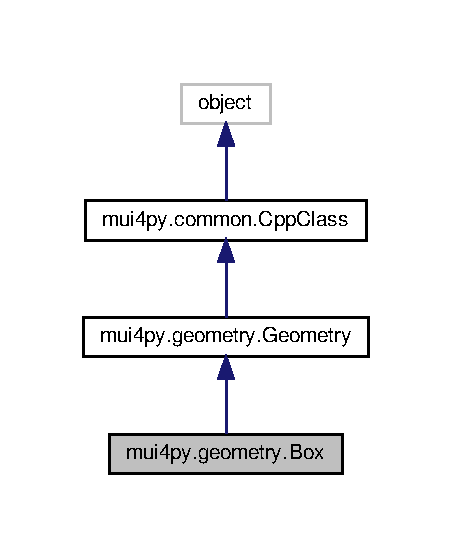
\includegraphics[width=217pt]{classmui4py_1_1geometry_1_1_box__inherit__graph}
\end{center}
\end{figure}


Collaboration diagram for mui4py.\+geometry.\+Box\+:
\nopagebreak
\begin{figure}[H]
\begin{center}
\leavevmode
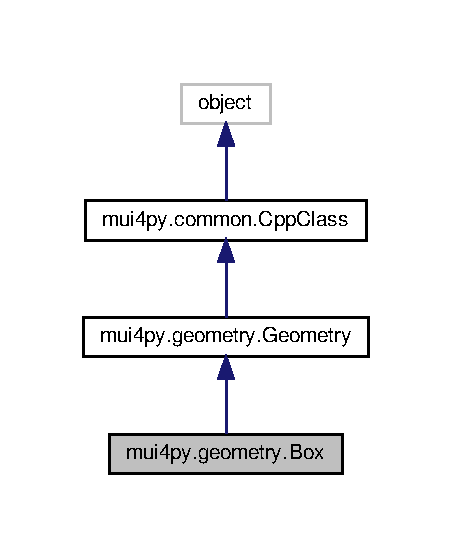
\includegraphics[width=217pt]{classmui4py_1_1geometry_1_1_box__coll__graph}
\end{center}
\end{figure}
\subsection*{Public Member Functions}
\begin{DoxyCompactItemize}
\item 
def \hyperlink{classmui4py_1_1geometry_1_1_box_a6f3bc905897566beee73c83c69b4d209}{\+\_\+\+\_\+init\+\_\+\+\_\+} (self, x1, x2)
\end{DoxyCompactItemize}
\subsection*{Additional Inherited Members}


\subsection{Constructor \& Destructor Documentation}
\mbox{\Hypertarget{classmui4py_1_1geometry_1_1_box_a6f3bc905897566beee73c83c69b4d209}\label{classmui4py_1_1geometry_1_1_box_a6f3bc905897566beee73c83c69b4d209}} 
\index{mui4py\+::geometry\+::\+Box@{mui4py\+::geometry\+::\+Box}!\+\_\+\+\_\+init\+\_\+\+\_\+@{\+\_\+\+\_\+init\+\_\+\+\_\+}}
\index{\+\_\+\+\_\+init\+\_\+\+\_\+@{\+\_\+\+\_\+init\+\_\+\+\_\+}!mui4py\+::geometry\+::\+Box@{mui4py\+::geometry\+::\+Box}}
\subsubsection{\texorpdfstring{\+\_\+\+\_\+init\+\_\+\+\_\+()}{\_\_init\_\_()}}
{\footnotesize\ttfamily def mui4py.\+geometry.\+Box.\+\_\+\+\_\+init\+\_\+\+\_\+ (\begin{DoxyParamCaption}\item[{}]{self,  }\item[{}]{x1,  }\item[{}]{x2 }\end{DoxyParamCaption})}



The documentation for this class was generated from the following file\+:\begin{DoxyCompactItemize}
\item 
wrappers/\+Python/mui4py/\hyperlink{geometry_8py}{geometry.\+py}\end{DoxyCompactItemize}

\hypertarget{classmui_1_1geometry_1_1box}{}\section{mui\+:\+:geometry\+:\+:box$<$ C\+O\+N\+F\+IG $>$ Class Template Reference}
\label{classmui_1_1geometry_1_1box}\index{mui\+::geometry\+::box$<$ C\+O\+N\+F\+I\+G $>$@{mui\+::geometry\+::box$<$ C\+O\+N\+F\+I\+G $>$}}


{\ttfamily \#include $<$geometry.\+h$>$}



Inheritance diagram for mui\+:\+:geometry\+:\+:box$<$ C\+O\+N\+F\+IG $>$\+:
\nopagebreak
\begin{figure}[H]
\begin{center}
\leavevmode
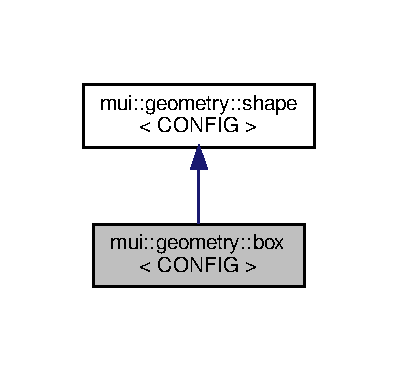
\includegraphics[width=191pt]{classmui_1_1geometry_1_1box__inherit__graph}
\end{center}
\end{figure}


Collaboration diagram for mui\+:\+:geometry\+:\+:box$<$ C\+O\+N\+F\+IG $>$\+:
\nopagebreak
\begin{figure}[H]
\begin{center}
\leavevmode
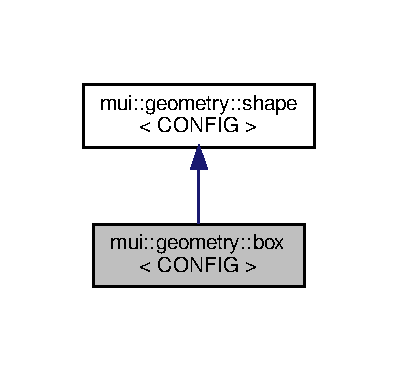
\includegraphics[width=191pt]{classmui_1_1geometry_1_1box__coll__graph}
\end{center}
\end{figure}
\subsection*{Public Member Functions}
\begin{DoxyCompactItemize}
\item 
\hyperlink{classmui_1_1geometry_1_1box_af95308237e008507cef0400b80539256}{box} ()=default
\item 
\hyperlink{classmui_1_1geometry_1_1box_a4b31077f538bd68d1120d4f1a458cd86}{box} (const coordinate\+\_\+type \&p1, const coordinate\+\_\+type \&p2)
\item 
coordinate\+\_\+type \hyperlink{classmui_1_1geometry_1_1box_a548b6ae064a454c01d23052105bd62f4}{get\+\_\+min} () const
\item 
coordinate\+\_\+type \& \hyperlink{classmui_1_1geometry_1_1box_a8bbabc54ec2b2d7491d8aff412431f40}{get\+\_\+min} ()
\item 
coordinate\+\_\+type \hyperlink{classmui_1_1geometry_1_1box_aac50a654e0e82789ba447ac9d360959d}{get\+\_\+max} () const
\item 
coordinate\+\_\+type \& \hyperlink{classmui_1_1geometry_1_1box_a421cca9434b9ae8dc7ed0bb7b2fed411}{get\+\_\+max} ()
\item 
\hyperlink{classmui_1_1geometry_1_1shape}{shape}$<$ C\+O\+N\+F\+IG $>$ $\ast$ \hyperlink{classmui_1_1geometry_1_1box_aa7422049fe305395107f9cfd04c804bf}{clone} () const
\item 
\hyperlink{namespacemui_1_1geometry_a5f311a343181e2f20482e5c9afb0f136}{shape\+\_\+type} \hyperlink{classmui_1_1geometry_1_1box_a88a57a405777e8f34e632030d725f7be}{type} () const noexcept
\item 
\hyperlink{classmui_1_1geometry_1_1box}{box}$<$ C\+O\+N\+F\+IG $>$ \hyperlink{classmui_1_1geometry_1_1box_a900ea59f5e2745d18664690dc52c642b}{bbox} () const
\item 
void \hyperlink{classmui_1_1geometry_1_1box_aea666920fb81b48c7561df7d7da8a0d6}{serialize} (\hyperlink{classmui_1_1ostream}{ostream} \&stream) const
\item 
void \hyperlink{classmui_1_1geometry_1_1box_a35467a9cfe92d36b2b232b796f7959e7}{deserialize} (\hyperlink{classmui_1_1istream}{istream} \&stream)
\end{DoxyCompactItemize}
\subsection*{Additional Inherited Members}


\subsection{Constructor \& Destructor Documentation}
\mbox{\Hypertarget{classmui_1_1geometry_1_1box_af95308237e008507cef0400b80539256}\label{classmui_1_1geometry_1_1box_af95308237e008507cef0400b80539256}} 
\index{mui\+::geometry\+::box@{mui\+::geometry\+::box}!box@{box}}
\index{box@{box}!mui\+::geometry\+::box@{mui\+::geometry\+::box}}
\subsubsection{\texorpdfstring{box()}{box()}\hspace{0.1cm}{\footnotesize\ttfamily [1/2]}}
{\footnotesize\ttfamily template$<$typename C\+O\+N\+F\+IG$>$ \\
\hyperlink{classmui_1_1geometry_1_1box}{mui\+::geometry\+::box}$<$ C\+O\+N\+F\+IG $>$\+::\hyperlink{classmui_1_1geometry_1_1box}{box} (\begin{DoxyParamCaption}{ }\end{DoxyParamCaption})\hspace{0.3cm}{\ttfamily [default]}}

\mbox{\Hypertarget{classmui_1_1geometry_1_1box_a4b31077f538bd68d1120d4f1a458cd86}\label{classmui_1_1geometry_1_1box_a4b31077f538bd68d1120d4f1a458cd86}} 
\index{mui\+::geometry\+::box@{mui\+::geometry\+::box}!box@{box}}
\index{box@{box}!mui\+::geometry\+::box@{mui\+::geometry\+::box}}
\subsubsection{\texorpdfstring{box()}{box()}\hspace{0.1cm}{\footnotesize\ttfamily [2/2]}}
{\footnotesize\ttfamily template$<$typename C\+O\+N\+F\+IG$>$ \\
\hyperlink{classmui_1_1geometry_1_1box}{mui\+::geometry\+::box}$<$ C\+O\+N\+F\+IG $>$\+::\hyperlink{classmui_1_1geometry_1_1box}{box} (\begin{DoxyParamCaption}\item[{const coordinate\+\_\+type \&}]{p1,  }\item[{const coordinate\+\_\+type \&}]{p2 }\end{DoxyParamCaption})\hspace{0.3cm}{\ttfamily [inline]}}



\subsection{Member Function Documentation}
\mbox{\Hypertarget{classmui_1_1geometry_1_1box_a900ea59f5e2745d18664690dc52c642b}\label{classmui_1_1geometry_1_1box_a900ea59f5e2745d18664690dc52c642b}} 
\index{mui\+::geometry\+::box@{mui\+::geometry\+::box}!bbox@{bbox}}
\index{bbox@{bbox}!mui\+::geometry\+::box@{mui\+::geometry\+::box}}
\subsubsection{\texorpdfstring{bbox()}{bbox()}}
{\footnotesize\ttfamily template$<$typename C\+O\+N\+F\+IG $>$ \\
\hyperlink{classmui_1_1geometry_1_1box}{box}$<$ C\+O\+N\+F\+IG $>$ \hyperlink{classmui_1_1geometry_1_1box}{mui\+::geometry\+::box}$<$ C\+O\+N\+F\+IG $>$\+::bbox (\begin{DoxyParamCaption}{ }\end{DoxyParamCaption}) const\hspace{0.3cm}{\ttfamily [virtual]}}



Implements \hyperlink{classmui_1_1geometry_1_1shape_adf598ec651ea425553bd8e617cac7430}{mui\+::geometry\+::shape$<$ C\+O\+N\+F\+I\+G $>$}.

\mbox{\Hypertarget{classmui_1_1geometry_1_1box_aa7422049fe305395107f9cfd04c804bf}\label{classmui_1_1geometry_1_1box_aa7422049fe305395107f9cfd04c804bf}} 
\index{mui\+::geometry\+::box@{mui\+::geometry\+::box}!clone@{clone}}
\index{clone@{clone}!mui\+::geometry\+::box@{mui\+::geometry\+::box}}
\subsubsection{\texorpdfstring{clone()}{clone()}}
{\footnotesize\ttfamily template$<$typename C\+O\+N\+F\+IG$>$ \\
\hyperlink{classmui_1_1geometry_1_1shape}{shape}$<$C\+O\+N\+F\+IG$>$$\ast$ \hyperlink{classmui_1_1geometry_1_1box}{mui\+::geometry\+::box}$<$ C\+O\+N\+F\+IG $>$\+::clone (\begin{DoxyParamCaption}{ }\end{DoxyParamCaption}) const\hspace{0.3cm}{\ttfamily [inline]}, {\ttfamily [virtual]}}



Implements \hyperlink{classmui_1_1geometry_1_1shape_a4d1307ebc40d462b13da89c811b3beb7}{mui\+::geometry\+::shape$<$ C\+O\+N\+F\+I\+G $>$}.

\mbox{\Hypertarget{classmui_1_1geometry_1_1box_a35467a9cfe92d36b2b232b796f7959e7}\label{classmui_1_1geometry_1_1box_a35467a9cfe92d36b2b232b796f7959e7}} 
\index{mui\+::geometry\+::box@{mui\+::geometry\+::box}!deserialize@{deserialize}}
\index{deserialize@{deserialize}!mui\+::geometry\+::box@{mui\+::geometry\+::box}}
\subsubsection{\texorpdfstring{deserialize()}{deserialize()}}
{\footnotesize\ttfamily template$<$typename C\+O\+N\+F\+IG$>$ \\
void \hyperlink{classmui_1_1geometry_1_1box}{mui\+::geometry\+::box}$<$ C\+O\+N\+F\+IG $>$\+::deserialize (\begin{DoxyParamCaption}\item[{\hyperlink{classmui_1_1istream}{istream} \&}]{stream }\end{DoxyParamCaption})\hspace{0.3cm}{\ttfamily [inline]}, {\ttfamily [virtual]}}



Implements \hyperlink{classmui_1_1geometry_1_1shape_ae68c7e1a1ae362abec52edad5489a1a9}{mui\+::geometry\+::shape$<$ C\+O\+N\+F\+I\+G $>$}.

\mbox{\Hypertarget{classmui_1_1geometry_1_1box_aac50a654e0e82789ba447ac9d360959d}\label{classmui_1_1geometry_1_1box_aac50a654e0e82789ba447ac9d360959d}} 
\index{mui\+::geometry\+::box@{mui\+::geometry\+::box}!get\+\_\+max@{get\+\_\+max}}
\index{get\+\_\+max@{get\+\_\+max}!mui\+::geometry\+::box@{mui\+::geometry\+::box}}
\subsubsection{\texorpdfstring{get\+\_\+max()}{get\_max()}\hspace{0.1cm}{\footnotesize\ttfamily [1/2]}}
{\footnotesize\ttfamily template$<$typename C\+O\+N\+F\+IG$>$ \\
coordinate\+\_\+type \hyperlink{classmui_1_1geometry_1_1box}{mui\+::geometry\+::box}$<$ C\+O\+N\+F\+IG $>$\+::get\+\_\+max (\begin{DoxyParamCaption}{ }\end{DoxyParamCaption}) const\hspace{0.3cm}{\ttfamily [inline]}}

\mbox{\Hypertarget{classmui_1_1geometry_1_1box_a421cca9434b9ae8dc7ed0bb7b2fed411}\label{classmui_1_1geometry_1_1box_a421cca9434b9ae8dc7ed0bb7b2fed411}} 
\index{mui\+::geometry\+::box@{mui\+::geometry\+::box}!get\+\_\+max@{get\+\_\+max}}
\index{get\+\_\+max@{get\+\_\+max}!mui\+::geometry\+::box@{mui\+::geometry\+::box}}
\subsubsection{\texorpdfstring{get\+\_\+max()}{get\_max()}\hspace{0.1cm}{\footnotesize\ttfamily [2/2]}}
{\footnotesize\ttfamily template$<$typename C\+O\+N\+F\+IG$>$ \\
coordinate\+\_\+type\& \hyperlink{classmui_1_1geometry_1_1box}{mui\+::geometry\+::box}$<$ C\+O\+N\+F\+IG $>$\+::get\+\_\+max (\begin{DoxyParamCaption}{ }\end{DoxyParamCaption})\hspace{0.3cm}{\ttfamily [inline]}}

\mbox{\Hypertarget{classmui_1_1geometry_1_1box_a548b6ae064a454c01d23052105bd62f4}\label{classmui_1_1geometry_1_1box_a548b6ae064a454c01d23052105bd62f4}} 
\index{mui\+::geometry\+::box@{mui\+::geometry\+::box}!get\+\_\+min@{get\+\_\+min}}
\index{get\+\_\+min@{get\+\_\+min}!mui\+::geometry\+::box@{mui\+::geometry\+::box}}
\subsubsection{\texorpdfstring{get\+\_\+min()}{get\_min()}\hspace{0.1cm}{\footnotesize\ttfamily [1/2]}}
{\footnotesize\ttfamily template$<$typename C\+O\+N\+F\+IG$>$ \\
coordinate\+\_\+type \hyperlink{classmui_1_1geometry_1_1box}{mui\+::geometry\+::box}$<$ C\+O\+N\+F\+IG $>$\+::get\+\_\+min (\begin{DoxyParamCaption}{ }\end{DoxyParamCaption}) const\hspace{0.3cm}{\ttfamily [inline]}}

\mbox{\Hypertarget{classmui_1_1geometry_1_1box_a8bbabc54ec2b2d7491d8aff412431f40}\label{classmui_1_1geometry_1_1box_a8bbabc54ec2b2d7491d8aff412431f40}} 
\index{mui\+::geometry\+::box@{mui\+::geometry\+::box}!get\+\_\+min@{get\+\_\+min}}
\index{get\+\_\+min@{get\+\_\+min}!mui\+::geometry\+::box@{mui\+::geometry\+::box}}
\subsubsection{\texorpdfstring{get\+\_\+min()}{get\_min()}\hspace{0.1cm}{\footnotesize\ttfamily [2/2]}}
{\footnotesize\ttfamily template$<$typename C\+O\+N\+F\+IG$>$ \\
coordinate\+\_\+type\& \hyperlink{classmui_1_1geometry_1_1box}{mui\+::geometry\+::box}$<$ C\+O\+N\+F\+IG $>$\+::get\+\_\+min (\begin{DoxyParamCaption}{ }\end{DoxyParamCaption})\hspace{0.3cm}{\ttfamily [inline]}}

\mbox{\Hypertarget{classmui_1_1geometry_1_1box_aea666920fb81b48c7561df7d7da8a0d6}\label{classmui_1_1geometry_1_1box_aea666920fb81b48c7561df7d7da8a0d6}} 
\index{mui\+::geometry\+::box@{mui\+::geometry\+::box}!serialize@{serialize}}
\index{serialize@{serialize}!mui\+::geometry\+::box@{mui\+::geometry\+::box}}
\subsubsection{\texorpdfstring{serialize()}{serialize()}}
{\footnotesize\ttfamily template$<$typename C\+O\+N\+F\+IG$>$ \\
void \hyperlink{classmui_1_1geometry_1_1box}{mui\+::geometry\+::box}$<$ C\+O\+N\+F\+IG $>$\+::serialize (\begin{DoxyParamCaption}\item[{\hyperlink{classmui_1_1ostream}{ostream} \&}]{stream }\end{DoxyParamCaption}) const\hspace{0.3cm}{\ttfamily [inline]}, {\ttfamily [virtual]}}



Implements \hyperlink{classmui_1_1geometry_1_1shape_ab1b2e763113b96dd0ae3deedfa0e7d22}{mui\+::geometry\+::shape$<$ C\+O\+N\+F\+I\+G $>$}.

\mbox{\Hypertarget{classmui_1_1geometry_1_1box_a88a57a405777e8f34e632030d725f7be}\label{classmui_1_1geometry_1_1box_a88a57a405777e8f34e632030d725f7be}} 
\index{mui\+::geometry\+::box@{mui\+::geometry\+::box}!type@{type}}
\index{type@{type}!mui\+::geometry\+::box@{mui\+::geometry\+::box}}
\subsubsection{\texorpdfstring{type()}{type()}}
{\footnotesize\ttfamily template$<$typename C\+O\+N\+F\+IG$>$ \\
\hyperlink{namespacemui_1_1geometry_a5f311a343181e2f20482e5c9afb0f136}{shape\+\_\+type} \hyperlink{classmui_1_1geometry_1_1box}{mui\+::geometry\+::box}$<$ C\+O\+N\+F\+IG $>$\+::type (\begin{DoxyParamCaption}{ }\end{DoxyParamCaption}) const\hspace{0.3cm}{\ttfamily [inline]}, {\ttfamily [virtual]}, {\ttfamily [noexcept]}}



Implements \hyperlink{classmui_1_1geometry_1_1shape_a4a0fe17b8ca5cc29e260cb38c9fcf8fe}{mui\+::geometry\+::shape$<$ C\+O\+N\+F\+I\+G $>$}.



The documentation for this class was generated from the following file\+:\begin{DoxyCompactItemize}
\item 
\hyperlink{geometry_8h}{geometry.\+h}\end{DoxyCompactItemize}

\hypertarget{classmui_1_1chrono__sampler__exact}{}\section{mui\+:\+:chrono\+\_\+sampler\+\_\+exact$<$ C\+O\+N\+F\+IG $>$ Class Template Reference}
\label{classmui_1_1chrono__sampler__exact}\index{mui\+::chrono\+\_\+sampler\+\_\+exact$<$ C\+O\+N\+F\+I\+G $>$@{mui\+::chrono\+\_\+sampler\+\_\+exact$<$ C\+O\+N\+F\+I\+G $>$}}


{\ttfamily \#include $<$chrono\+\_\+sampler\+\_\+exact.\+h$>$}

\subsection*{Public Types}
\begin{DoxyCompactItemize}
\item 
using \hyperlink{classmui_1_1chrono__sampler__exact_ad55f9693aa8d6a9652d9b51639463d84}{R\+E\+AL} = typename C\+O\+N\+F\+I\+G\+::\+R\+E\+AL
\item 
using \hyperlink{classmui_1_1chrono__sampler__exact_a1765b8d8fec705157ac526e186727e9a}{I\+NT} = typename C\+O\+N\+F\+I\+G\+::\+I\+NT
\item 
using \hyperlink{classmui_1_1chrono__sampler__exact_a5f9178b26822fe901f8a1e97ada68d95}{time\+\_\+type} = typename C\+O\+N\+F\+I\+G\+::time\+\_\+type
\end{DoxyCompactItemize}
\subsection*{Public Member Functions}
\begin{DoxyCompactItemize}
\item 
\hyperlink{classmui_1_1chrono__sampler__exact_ad1293d1816ab17b696ed8c1d665c9cae}{chrono\+\_\+sampler\+\_\+exact} (\hyperlink{classmui_1_1chrono__sampler__exact_a5f9178b26822fe901f8a1e97ada68d95}{time\+\_\+type} tol=\hyperlink{classmui_1_1chrono__sampler__exact_a5f9178b26822fe901f8a1e97ada68d95}{time\+\_\+type}(std\+::numeric\+\_\+limits$<$ \hyperlink{classmui_1_1chrono__sampler__exact_a5f9178b26822fe901f8a1e97ada68d95}{time\+\_\+type} $>$\+::epsilon()))
\item 
{\footnotesize template$<$typename T\+Y\+PE $>$ }\\T\+Y\+PE \hyperlink{classmui_1_1chrono__sampler__exact_a8bef847fd06c25c4f8869b0a962a6193}{filter} (\hyperlink{classmui_1_1chrono__sampler__exact_a5f9178b26822fe901f8a1e97ada68d95}{time\+\_\+type} focus, const std\+::vector$<$ std\+::pair$<$ \hyperlink{classmui_1_1chrono__sampler__exact_a5f9178b26822fe901f8a1e97ada68d95}{time\+\_\+type}, T\+Y\+PE $>$ $>$ \&points) const
\item 
\hyperlink{classmui_1_1chrono__sampler__exact_a5f9178b26822fe901f8a1e97ada68d95}{time\+\_\+type} \hyperlink{classmui_1_1chrono__sampler__exact_a1743254818f1f6fb5ef3eff5e7eef0c6}{get\+\_\+upper\+\_\+bound} (\hyperlink{classmui_1_1chrono__sampler__exact_a5f9178b26822fe901f8a1e97ada68d95}{time\+\_\+type} focus) const
\item 
\hyperlink{classmui_1_1chrono__sampler__exact_a5f9178b26822fe901f8a1e97ada68d95}{time\+\_\+type} \hyperlink{classmui_1_1chrono__sampler__exact_a1297822afb4c05df461926a4d234a61d}{get\+\_\+lower\+\_\+bound} (\hyperlink{classmui_1_1chrono__sampler__exact_a5f9178b26822fe901f8a1e97ada68d95}{time\+\_\+type} focus) const
\end{DoxyCompactItemize}


\subsection{Member Typedef Documentation}
\mbox{\Hypertarget{classmui_1_1chrono__sampler__exact_a1765b8d8fec705157ac526e186727e9a}\label{classmui_1_1chrono__sampler__exact_a1765b8d8fec705157ac526e186727e9a}} 
\index{mui\+::chrono\+\_\+sampler\+\_\+exact@{mui\+::chrono\+\_\+sampler\+\_\+exact}!I\+NT@{I\+NT}}
\index{I\+NT@{I\+NT}!mui\+::chrono\+\_\+sampler\+\_\+exact@{mui\+::chrono\+\_\+sampler\+\_\+exact}}
\subsubsection{\texorpdfstring{I\+NT}{INT}}
{\footnotesize\ttfamily template$<$typename C\+O\+N\+F\+IG  = default\+\_\+config$>$ \\
using \hyperlink{classmui_1_1chrono__sampler__exact}{mui\+::chrono\+\_\+sampler\+\_\+exact}$<$ C\+O\+N\+F\+IG $>$\+::\hyperlink{classmui_1_1chrono__sampler__exact_a1765b8d8fec705157ac526e186727e9a}{I\+NT} =  typename C\+O\+N\+F\+I\+G\+::\+I\+NT}

\mbox{\Hypertarget{classmui_1_1chrono__sampler__exact_ad55f9693aa8d6a9652d9b51639463d84}\label{classmui_1_1chrono__sampler__exact_ad55f9693aa8d6a9652d9b51639463d84}} 
\index{mui\+::chrono\+\_\+sampler\+\_\+exact@{mui\+::chrono\+\_\+sampler\+\_\+exact}!R\+E\+AL@{R\+E\+AL}}
\index{R\+E\+AL@{R\+E\+AL}!mui\+::chrono\+\_\+sampler\+\_\+exact@{mui\+::chrono\+\_\+sampler\+\_\+exact}}
\subsubsection{\texorpdfstring{R\+E\+AL}{REAL}}
{\footnotesize\ttfamily template$<$typename C\+O\+N\+F\+IG  = default\+\_\+config$>$ \\
using \hyperlink{classmui_1_1chrono__sampler__exact}{mui\+::chrono\+\_\+sampler\+\_\+exact}$<$ C\+O\+N\+F\+IG $>$\+::\hyperlink{classmui_1_1chrono__sampler__exact_ad55f9693aa8d6a9652d9b51639463d84}{R\+E\+AL} =  typename C\+O\+N\+F\+I\+G\+::\+R\+E\+AL}

\mbox{\Hypertarget{classmui_1_1chrono__sampler__exact_a5f9178b26822fe901f8a1e97ada68d95}\label{classmui_1_1chrono__sampler__exact_a5f9178b26822fe901f8a1e97ada68d95}} 
\index{mui\+::chrono\+\_\+sampler\+\_\+exact@{mui\+::chrono\+\_\+sampler\+\_\+exact}!time\+\_\+type@{time\+\_\+type}}
\index{time\+\_\+type@{time\+\_\+type}!mui\+::chrono\+\_\+sampler\+\_\+exact@{mui\+::chrono\+\_\+sampler\+\_\+exact}}
\subsubsection{\texorpdfstring{time\+\_\+type}{time\_type}}
{\footnotesize\ttfamily template$<$typename C\+O\+N\+F\+IG  = default\+\_\+config$>$ \\
using \hyperlink{classmui_1_1chrono__sampler__exact}{mui\+::chrono\+\_\+sampler\+\_\+exact}$<$ C\+O\+N\+F\+IG $>$\+::\hyperlink{classmui_1_1chrono__sampler__exact_a5f9178b26822fe901f8a1e97ada68d95}{time\+\_\+type} =  typename C\+O\+N\+F\+I\+G\+::time\+\_\+type}



\subsection{Constructor \& Destructor Documentation}
\mbox{\Hypertarget{classmui_1_1chrono__sampler__exact_ad1293d1816ab17b696ed8c1d665c9cae}\label{classmui_1_1chrono__sampler__exact_ad1293d1816ab17b696ed8c1d665c9cae}} 
\index{mui\+::chrono\+\_\+sampler\+\_\+exact@{mui\+::chrono\+\_\+sampler\+\_\+exact}!chrono\+\_\+sampler\+\_\+exact@{chrono\+\_\+sampler\+\_\+exact}}
\index{chrono\+\_\+sampler\+\_\+exact@{chrono\+\_\+sampler\+\_\+exact}!mui\+::chrono\+\_\+sampler\+\_\+exact@{mui\+::chrono\+\_\+sampler\+\_\+exact}}
\subsubsection{\texorpdfstring{chrono\+\_\+sampler\+\_\+exact()}{chrono\_sampler\_exact()}}
{\footnotesize\ttfamily template$<$typename C\+O\+N\+F\+IG  = default\+\_\+config$>$ \\
\hyperlink{classmui_1_1chrono__sampler__exact}{mui\+::chrono\+\_\+sampler\+\_\+exact}$<$ C\+O\+N\+F\+IG $>$\+::\hyperlink{classmui_1_1chrono__sampler__exact}{chrono\+\_\+sampler\+\_\+exact} (\begin{DoxyParamCaption}\item[{\hyperlink{classmui_1_1chrono__sampler__exact_a5f9178b26822fe901f8a1e97ada68d95}{time\+\_\+type}}]{tol = {\ttfamily \hyperlink{classmui_1_1chrono__sampler__exact_a5f9178b26822fe901f8a1e97ada68d95}{time\+\_\+type}(std\+:\+:numeric\+\_\+limits$<$\hyperlink{classmui_1_1chrono__sampler__exact_a5f9178b26822fe901f8a1e97ada68d95}{time\+\_\+type}$>$\+:\+:epsilon())} }\end{DoxyParamCaption})\hspace{0.3cm}{\ttfamily [inline]}}



\subsection{Member Function Documentation}
\mbox{\Hypertarget{classmui_1_1chrono__sampler__exact_a8bef847fd06c25c4f8869b0a962a6193}\label{classmui_1_1chrono__sampler__exact_a8bef847fd06c25c4f8869b0a962a6193}} 
\index{mui\+::chrono\+\_\+sampler\+\_\+exact@{mui\+::chrono\+\_\+sampler\+\_\+exact}!filter@{filter}}
\index{filter@{filter}!mui\+::chrono\+\_\+sampler\+\_\+exact@{mui\+::chrono\+\_\+sampler\+\_\+exact}}
\subsubsection{\texorpdfstring{filter()}{filter()}}
{\footnotesize\ttfamily template$<$typename C\+O\+N\+F\+IG  = default\+\_\+config$>$ \\
template$<$typename T\+Y\+PE $>$ \\
T\+Y\+PE \hyperlink{classmui_1_1chrono__sampler__exact}{mui\+::chrono\+\_\+sampler\+\_\+exact}$<$ C\+O\+N\+F\+IG $>$\+::filter (\begin{DoxyParamCaption}\item[{\hyperlink{classmui_1_1chrono__sampler__exact_a5f9178b26822fe901f8a1e97ada68d95}{time\+\_\+type}}]{focus,  }\item[{const std\+::vector$<$ std\+::pair$<$ \hyperlink{classmui_1_1chrono__sampler__exact_a5f9178b26822fe901f8a1e97ada68d95}{time\+\_\+type}, T\+Y\+PE $>$ $>$ \&}]{points }\end{DoxyParamCaption}) const\hspace{0.3cm}{\ttfamily [inline]}}

\mbox{\Hypertarget{classmui_1_1chrono__sampler__exact_a1297822afb4c05df461926a4d234a61d}\label{classmui_1_1chrono__sampler__exact_a1297822afb4c05df461926a4d234a61d}} 
\index{mui\+::chrono\+\_\+sampler\+\_\+exact@{mui\+::chrono\+\_\+sampler\+\_\+exact}!get\+\_\+lower\+\_\+bound@{get\+\_\+lower\+\_\+bound}}
\index{get\+\_\+lower\+\_\+bound@{get\+\_\+lower\+\_\+bound}!mui\+::chrono\+\_\+sampler\+\_\+exact@{mui\+::chrono\+\_\+sampler\+\_\+exact}}
\subsubsection{\texorpdfstring{get\+\_\+lower\+\_\+bound()}{get\_lower\_bound()}}
{\footnotesize\ttfamily template$<$typename C\+O\+N\+F\+IG  = default\+\_\+config$>$ \\
\hyperlink{classmui_1_1chrono__sampler__exact_a5f9178b26822fe901f8a1e97ada68d95}{time\+\_\+type} \hyperlink{classmui_1_1chrono__sampler__exact}{mui\+::chrono\+\_\+sampler\+\_\+exact}$<$ C\+O\+N\+F\+IG $>$\+::get\+\_\+lower\+\_\+bound (\begin{DoxyParamCaption}\item[{\hyperlink{classmui_1_1chrono__sampler__exact_a5f9178b26822fe901f8a1e97ada68d95}{time\+\_\+type}}]{focus }\end{DoxyParamCaption}) const\hspace{0.3cm}{\ttfamily [inline]}}

\mbox{\Hypertarget{classmui_1_1chrono__sampler__exact_a1743254818f1f6fb5ef3eff5e7eef0c6}\label{classmui_1_1chrono__sampler__exact_a1743254818f1f6fb5ef3eff5e7eef0c6}} 
\index{mui\+::chrono\+\_\+sampler\+\_\+exact@{mui\+::chrono\+\_\+sampler\+\_\+exact}!get\+\_\+upper\+\_\+bound@{get\+\_\+upper\+\_\+bound}}
\index{get\+\_\+upper\+\_\+bound@{get\+\_\+upper\+\_\+bound}!mui\+::chrono\+\_\+sampler\+\_\+exact@{mui\+::chrono\+\_\+sampler\+\_\+exact}}
\subsubsection{\texorpdfstring{get\+\_\+upper\+\_\+bound()}{get\_upper\_bound()}}
{\footnotesize\ttfamily template$<$typename C\+O\+N\+F\+IG  = default\+\_\+config$>$ \\
\hyperlink{classmui_1_1chrono__sampler__exact_a5f9178b26822fe901f8a1e97ada68d95}{time\+\_\+type} \hyperlink{classmui_1_1chrono__sampler__exact}{mui\+::chrono\+\_\+sampler\+\_\+exact}$<$ C\+O\+N\+F\+IG $>$\+::get\+\_\+upper\+\_\+bound (\begin{DoxyParamCaption}\item[{\hyperlink{classmui_1_1chrono__sampler__exact_a5f9178b26822fe901f8a1e97ada68d95}{time\+\_\+type}}]{focus }\end{DoxyParamCaption}) const\hspace{0.3cm}{\ttfamily [inline]}}



The documentation for this class was generated from the following file\+:\begin{DoxyCompactItemize}
\item 
chrono\+\_\+samplers/\hyperlink{chrono__sampler__exact_8h}{chrono\+\_\+sampler\+\_\+exact.\+h}\end{DoxyCompactItemize}

\hypertarget{classmui_1_1chrono__sampler__gauss}{}\section{mui\+:\+:chrono\+\_\+sampler\+\_\+gauss$<$ C\+O\+N\+F\+IG $>$ Class Template Reference}
\label{classmui_1_1chrono__sampler__gauss}\index{mui\+::chrono\+\_\+sampler\+\_\+gauss$<$ C\+O\+N\+F\+I\+G $>$@{mui\+::chrono\+\_\+sampler\+\_\+gauss$<$ C\+O\+N\+F\+I\+G $>$}}


{\ttfamily \#include $<$chrono\+\_\+sampler\+\_\+gauss.\+h$>$}

\subsection*{Public Types}
\begin{DoxyCompactItemize}
\item 
using \hyperlink{classmui_1_1chrono__sampler__gauss_acb55ad8350ad77bd80ea3979bc01f7a5}{R\+E\+AL} = typename C\+O\+N\+F\+I\+G\+::\+R\+E\+AL
\item 
using \hyperlink{classmui_1_1chrono__sampler__gauss_a86da50872efe4ac7b75234c463e716bf}{I\+NT} = typename C\+O\+N\+F\+I\+G\+::\+I\+NT
\item 
using \hyperlink{classmui_1_1chrono__sampler__gauss_accb8778472734fd419da15b26e087a41}{time\+\_\+type} = typename C\+O\+N\+F\+I\+G\+::time\+\_\+type
\end{DoxyCompactItemize}
\subsection*{Public Member Functions}
\begin{DoxyCompactItemize}
\item 
\hyperlink{classmui_1_1chrono__sampler__gauss_a0f89e81a457ebb15623fc4d0ad25cea5}{chrono\+\_\+sampler\+\_\+gauss} (\hyperlink{classmui_1_1chrono__sampler__gauss_accb8778472734fd419da15b26e087a41}{time\+\_\+type} newcutoff, \hyperlink{classmui_1_1chrono__sampler__gauss_acb55ad8350ad77bd80ea3979bc01f7a5}{R\+E\+AL} newsigma)
\item 
{\footnotesize template$<$typename T\+Y\+PE $>$ }\\T\+Y\+PE \hyperlink{classmui_1_1chrono__sampler__gauss_a6757bf02147d08582cc5f16910ac3a91}{filter} (\hyperlink{classmui_1_1chrono__sampler__gauss_accb8778472734fd419da15b26e087a41}{time\+\_\+type} focus, const std\+::vector$<$ std\+::pair$<$ \hyperlink{classmui_1_1chrono__sampler__gauss_accb8778472734fd419da15b26e087a41}{time\+\_\+type}, T\+Y\+PE $>$ $>$ \&points) const
\item 
\hyperlink{classmui_1_1chrono__sampler__gauss_accb8778472734fd419da15b26e087a41}{time\+\_\+type} \hyperlink{classmui_1_1chrono__sampler__gauss_a8fb552103746c9a1d430dbb6125eadd3}{get\+\_\+upper\+\_\+bound} (\hyperlink{classmui_1_1chrono__sampler__gauss_accb8778472734fd419da15b26e087a41}{time\+\_\+type} focus) const
\item 
\hyperlink{classmui_1_1chrono__sampler__gauss_accb8778472734fd419da15b26e087a41}{time\+\_\+type} \hyperlink{classmui_1_1chrono__sampler__gauss_aea11a50917c7bae0a75b9b4fafc31911}{get\+\_\+lower\+\_\+bound} (\hyperlink{classmui_1_1chrono__sampler__gauss_accb8778472734fd419da15b26e087a41}{time\+\_\+type} focus) const
\item 
\hyperlink{classmui_1_1chrono__sampler__gauss_accb8778472734fd419da15b26e087a41}{time\+\_\+type} \hyperlink{classmui_1_1chrono__sampler__gauss_ad19e8fc5d18b5568ab4c8f52fe518336}{tolerance} () const
\end{DoxyCompactItemize}
\subsection*{Protected Attributes}
\begin{DoxyCompactItemize}
\item 
\hyperlink{classmui_1_1chrono__sampler__gauss_accb8778472734fd419da15b26e087a41}{time\+\_\+type} \hyperlink{classmui_1_1chrono__sampler__gauss_a279b7de2f573d7a6f7316b4748eb3ec4}{cutoff}
\item 
\hyperlink{classmui_1_1chrono__sampler__gauss_acb55ad8350ad77bd80ea3979bc01f7a5}{R\+E\+AL} \hyperlink{classmui_1_1chrono__sampler__gauss_a10b2a032bbbebecf559a0fe3fbf92714}{sigma}
\end{DoxyCompactItemize}


\subsection{Member Typedef Documentation}
\mbox{\Hypertarget{classmui_1_1chrono__sampler__gauss_a86da50872efe4ac7b75234c463e716bf}\label{classmui_1_1chrono__sampler__gauss_a86da50872efe4ac7b75234c463e716bf}} 
\index{mui\+::chrono\+\_\+sampler\+\_\+gauss@{mui\+::chrono\+\_\+sampler\+\_\+gauss}!I\+NT@{I\+NT}}
\index{I\+NT@{I\+NT}!mui\+::chrono\+\_\+sampler\+\_\+gauss@{mui\+::chrono\+\_\+sampler\+\_\+gauss}}
\subsubsection{\texorpdfstring{I\+NT}{INT}}
{\footnotesize\ttfamily template$<$typename C\+O\+N\+F\+IG  = default\+\_\+config$>$ \\
using \hyperlink{classmui_1_1chrono__sampler__gauss}{mui\+::chrono\+\_\+sampler\+\_\+gauss}$<$ C\+O\+N\+F\+IG $>$\+::\hyperlink{classmui_1_1chrono__sampler__gauss_a86da50872efe4ac7b75234c463e716bf}{I\+NT} =  typename C\+O\+N\+F\+I\+G\+::\+I\+NT}

\mbox{\Hypertarget{classmui_1_1chrono__sampler__gauss_acb55ad8350ad77bd80ea3979bc01f7a5}\label{classmui_1_1chrono__sampler__gauss_acb55ad8350ad77bd80ea3979bc01f7a5}} 
\index{mui\+::chrono\+\_\+sampler\+\_\+gauss@{mui\+::chrono\+\_\+sampler\+\_\+gauss}!R\+E\+AL@{R\+E\+AL}}
\index{R\+E\+AL@{R\+E\+AL}!mui\+::chrono\+\_\+sampler\+\_\+gauss@{mui\+::chrono\+\_\+sampler\+\_\+gauss}}
\subsubsection{\texorpdfstring{R\+E\+AL}{REAL}}
{\footnotesize\ttfamily template$<$typename C\+O\+N\+F\+IG  = default\+\_\+config$>$ \\
using \hyperlink{classmui_1_1chrono__sampler__gauss}{mui\+::chrono\+\_\+sampler\+\_\+gauss}$<$ C\+O\+N\+F\+IG $>$\+::\hyperlink{classmui_1_1chrono__sampler__gauss_acb55ad8350ad77bd80ea3979bc01f7a5}{R\+E\+AL} =  typename C\+O\+N\+F\+I\+G\+::\+R\+E\+AL}

\mbox{\Hypertarget{classmui_1_1chrono__sampler__gauss_accb8778472734fd419da15b26e087a41}\label{classmui_1_1chrono__sampler__gauss_accb8778472734fd419da15b26e087a41}} 
\index{mui\+::chrono\+\_\+sampler\+\_\+gauss@{mui\+::chrono\+\_\+sampler\+\_\+gauss}!time\+\_\+type@{time\+\_\+type}}
\index{time\+\_\+type@{time\+\_\+type}!mui\+::chrono\+\_\+sampler\+\_\+gauss@{mui\+::chrono\+\_\+sampler\+\_\+gauss}}
\subsubsection{\texorpdfstring{time\+\_\+type}{time\_type}}
{\footnotesize\ttfamily template$<$typename C\+O\+N\+F\+IG  = default\+\_\+config$>$ \\
using \hyperlink{classmui_1_1chrono__sampler__gauss}{mui\+::chrono\+\_\+sampler\+\_\+gauss}$<$ C\+O\+N\+F\+IG $>$\+::\hyperlink{classmui_1_1chrono__sampler__gauss_accb8778472734fd419da15b26e087a41}{time\+\_\+type} =  typename C\+O\+N\+F\+I\+G\+::time\+\_\+type}



\subsection{Constructor \& Destructor Documentation}
\mbox{\Hypertarget{classmui_1_1chrono__sampler__gauss_a0f89e81a457ebb15623fc4d0ad25cea5}\label{classmui_1_1chrono__sampler__gauss_a0f89e81a457ebb15623fc4d0ad25cea5}} 
\index{mui\+::chrono\+\_\+sampler\+\_\+gauss@{mui\+::chrono\+\_\+sampler\+\_\+gauss}!chrono\+\_\+sampler\+\_\+gauss@{chrono\+\_\+sampler\+\_\+gauss}}
\index{chrono\+\_\+sampler\+\_\+gauss@{chrono\+\_\+sampler\+\_\+gauss}!mui\+::chrono\+\_\+sampler\+\_\+gauss@{mui\+::chrono\+\_\+sampler\+\_\+gauss}}
\subsubsection{\texorpdfstring{chrono\+\_\+sampler\+\_\+gauss()}{chrono\_sampler\_gauss()}}
{\footnotesize\ttfamily template$<$typename C\+O\+N\+F\+IG  = default\+\_\+config$>$ \\
\hyperlink{classmui_1_1chrono__sampler__gauss}{mui\+::chrono\+\_\+sampler\+\_\+gauss}$<$ C\+O\+N\+F\+IG $>$\+::\hyperlink{classmui_1_1chrono__sampler__gauss}{chrono\+\_\+sampler\+\_\+gauss} (\begin{DoxyParamCaption}\item[{\hyperlink{classmui_1_1chrono__sampler__gauss_accb8778472734fd419da15b26e087a41}{time\+\_\+type}}]{newcutoff,  }\item[{\hyperlink{classmui_1_1chrono__sampler__gauss_acb55ad8350ad77bd80ea3979bc01f7a5}{R\+E\+AL}}]{newsigma }\end{DoxyParamCaption})\hspace{0.3cm}{\ttfamily [inline]}}



\subsection{Member Function Documentation}
\mbox{\Hypertarget{classmui_1_1chrono__sampler__gauss_a6757bf02147d08582cc5f16910ac3a91}\label{classmui_1_1chrono__sampler__gauss_a6757bf02147d08582cc5f16910ac3a91}} 
\index{mui\+::chrono\+\_\+sampler\+\_\+gauss@{mui\+::chrono\+\_\+sampler\+\_\+gauss}!filter@{filter}}
\index{filter@{filter}!mui\+::chrono\+\_\+sampler\+\_\+gauss@{mui\+::chrono\+\_\+sampler\+\_\+gauss}}
\subsubsection{\texorpdfstring{filter()}{filter()}}
{\footnotesize\ttfamily template$<$typename C\+O\+N\+F\+IG  = default\+\_\+config$>$ \\
template$<$typename T\+Y\+PE $>$ \\
T\+Y\+PE \hyperlink{classmui_1_1chrono__sampler__gauss}{mui\+::chrono\+\_\+sampler\+\_\+gauss}$<$ C\+O\+N\+F\+IG $>$\+::filter (\begin{DoxyParamCaption}\item[{\hyperlink{classmui_1_1chrono__sampler__gauss_accb8778472734fd419da15b26e087a41}{time\+\_\+type}}]{focus,  }\item[{const std\+::vector$<$ std\+::pair$<$ \hyperlink{classmui_1_1chrono__sampler__gauss_accb8778472734fd419da15b26e087a41}{time\+\_\+type}, T\+Y\+PE $>$ $>$ \&}]{points }\end{DoxyParamCaption}) const\hspace{0.3cm}{\ttfamily [inline]}}

\mbox{\Hypertarget{classmui_1_1chrono__sampler__gauss_aea11a50917c7bae0a75b9b4fafc31911}\label{classmui_1_1chrono__sampler__gauss_aea11a50917c7bae0a75b9b4fafc31911}} 
\index{mui\+::chrono\+\_\+sampler\+\_\+gauss@{mui\+::chrono\+\_\+sampler\+\_\+gauss}!get\+\_\+lower\+\_\+bound@{get\+\_\+lower\+\_\+bound}}
\index{get\+\_\+lower\+\_\+bound@{get\+\_\+lower\+\_\+bound}!mui\+::chrono\+\_\+sampler\+\_\+gauss@{mui\+::chrono\+\_\+sampler\+\_\+gauss}}
\subsubsection{\texorpdfstring{get\+\_\+lower\+\_\+bound()}{get\_lower\_bound()}}
{\footnotesize\ttfamily template$<$typename C\+O\+N\+F\+IG  = default\+\_\+config$>$ \\
\hyperlink{classmui_1_1chrono__sampler__gauss_accb8778472734fd419da15b26e087a41}{time\+\_\+type} \hyperlink{classmui_1_1chrono__sampler__gauss}{mui\+::chrono\+\_\+sampler\+\_\+gauss}$<$ C\+O\+N\+F\+IG $>$\+::get\+\_\+lower\+\_\+bound (\begin{DoxyParamCaption}\item[{\hyperlink{classmui_1_1chrono__sampler__gauss_accb8778472734fd419da15b26e087a41}{time\+\_\+type}}]{focus }\end{DoxyParamCaption}) const\hspace{0.3cm}{\ttfamily [inline]}}

\mbox{\Hypertarget{classmui_1_1chrono__sampler__gauss_a8fb552103746c9a1d430dbb6125eadd3}\label{classmui_1_1chrono__sampler__gauss_a8fb552103746c9a1d430dbb6125eadd3}} 
\index{mui\+::chrono\+\_\+sampler\+\_\+gauss@{mui\+::chrono\+\_\+sampler\+\_\+gauss}!get\+\_\+upper\+\_\+bound@{get\+\_\+upper\+\_\+bound}}
\index{get\+\_\+upper\+\_\+bound@{get\+\_\+upper\+\_\+bound}!mui\+::chrono\+\_\+sampler\+\_\+gauss@{mui\+::chrono\+\_\+sampler\+\_\+gauss}}
\subsubsection{\texorpdfstring{get\+\_\+upper\+\_\+bound()}{get\_upper\_bound()}}
{\footnotesize\ttfamily template$<$typename C\+O\+N\+F\+IG  = default\+\_\+config$>$ \\
\hyperlink{classmui_1_1chrono__sampler__gauss_accb8778472734fd419da15b26e087a41}{time\+\_\+type} \hyperlink{classmui_1_1chrono__sampler__gauss}{mui\+::chrono\+\_\+sampler\+\_\+gauss}$<$ C\+O\+N\+F\+IG $>$\+::get\+\_\+upper\+\_\+bound (\begin{DoxyParamCaption}\item[{\hyperlink{classmui_1_1chrono__sampler__gauss_accb8778472734fd419da15b26e087a41}{time\+\_\+type}}]{focus }\end{DoxyParamCaption}) const\hspace{0.3cm}{\ttfamily [inline]}}

\mbox{\Hypertarget{classmui_1_1chrono__sampler__gauss_ad19e8fc5d18b5568ab4c8f52fe518336}\label{classmui_1_1chrono__sampler__gauss_ad19e8fc5d18b5568ab4c8f52fe518336}} 
\index{mui\+::chrono\+\_\+sampler\+\_\+gauss@{mui\+::chrono\+\_\+sampler\+\_\+gauss}!tolerance@{tolerance}}
\index{tolerance@{tolerance}!mui\+::chrono\+\_\+sampler\+\_\+gauss@{mui\+::chrono\+\_\+sampler\+\_\+gauss}}
\subsubsection{\texorpdfstring{tolerance()}{tolerance()}}
{\footnotesize\ttfamily template$<$typename C\+O\+N\+F\+IG  = default\+\_\+config$>$ \\
\hyperlink{classmui_1_1chrono__sampler__gauss_accb8778472734fd419da15b26e087a41}{time\+\_\+type} \hyperlink{classmui_1_1chrono__sampler__gauss}{mui\+::chrono\+\_\+sampler\+\_\+gauss}$<$ C\+O\+N\+F\+IG $>$\+::tolerance (\begin{DoxyParamCaption}{ }\end{DoxyParamCaption}) const\hspace{0.3cm}{\ttfamily [inline]}}



\subsection{Member Data Documentation}
\mbox{\Hypertarget{classmui_1_1chrono__sampler__gauss_a279b7de2f573d7a6f7316b4748eb3ec4}\label{classmui_1_1chrono__sampler__gauss_a279b7de2f573d7a6f7316b4748eb3ec4}} 
\index{mui\+::chrono\+\_\+sampler\+\_\+gauss@{mui\+::chrono\+\_\+sampler\+\_\+gauss}!cutoff@{cutoff}}
\index{cutoff@{cutoff}!mui\+::chrono\+\_\+sampler\+\_\+gauss@{mui\+::chrono\+\_\+sampler\+\_\+gauss}}
\subsubsection{\texorpdfstring{cutoff}{cutoff}}
{\footnotesize\ttfamily template$<$typename C\+O\+N\+F\+IG  = default\+\_\+config$>$ \\
\hyperlink{classmui_1_1chrono__sampler__gauss_accb8778472734fd419da15b26e087a41}{time\+\_\+type} \hyperlink{classmui_1_1chrono__sampler__gauss}{mui\+::chrono\+\_\+sampler\+\_\+gauss}$<$ C\+O\+N\+F\+IG $>$\+::cutoff\hspace{0.3cm}{\ttfamily [protected]}}

\mbox{\Hypertarget{classmui_1_1chrono__sampler__gauss_a10b2a032bbbebecf559a0fe3fbf92714}\label{classmui_1_1chrono__sampler__gauss_a10b2a032bbbebecf559a0fe3fbf92714}} 
\index{mui\+::chrono\+\_\+sampler\+\_\+gauss@{mui\+::chrono\+\_\+sampler\+\_\+gauss}!sigma@{sigma}}
\index{sigma@{sigma}!mui\+::chrono\+\_\+sampler\+\_\+gauss@{mui\+::chrono\+\_\+sampler\+\_\+gauss}}
\subsubsection{\texorpdfstring{sigma}{sigma}}
{\footnotesize\ttfamily template$<$typename C\+O\+N\+F\+IG  = default\+\_\+config$>$ \\
\hyperlink{classmui_1_1chrono__sampler__gauss_acb55ad8350ad77bd80ea3979bc01f7a5}{R\+E\+AL} \hyperlink{classmui_1_1chrono__sampler__gauss}{mui\+::chrono\+\_\+sampler\+\_\+gauss}$<$ C\+O\+N\+F\+IG $>$\+::sigma\hspace{0.3cm}{\ttfamily [protected]}}



The documentation for this class was generated from the following file\+:\begin{DoxyCompactItemize}
\item 
chrono\+\_\+samplers/\hyperlink{chrono__sampler__gauss_8h}{chrono\+\_\+sampler\+\_\+gauss.\+h}\end{DoxyCompactItemize}

\hypertarget{classmui_1_1chrono__sampler__mean}{}\section{mui\+:\+:chrono\+\_\+sampler\+\_\+mean$<$ C\+O\+N\+F\+IG $>$ Class Template Reference}
\label{classmui_1_1chrono__sampler__mean}\index{mui\+::chrono\+\_\+sampler\+\_\+mean$<$ C\+O\+N\+F\+I\+G $>$@{mui\+::chrono\+\_\+sampler\+\_\+mean$<$ C\+O\+N\+F\+I\+G $>$}}


{\ttfamily \#include $<$chrono\+\_\+sampler\+\_\+mean.\+h$>$}

\subsection*{Public Types}
\begin{DoxyCompactItemize}
\item 
using \hyperlink{classmui_1_1chrono__sampler__mean_a31c93d26c0a7b8026ef9c3b0d0ddc5d2}{R\+E\+AL} = typename C\+O\+N\+F\+I\+G\+::\+R\+E\+AL
\item 
using \hyperlink{classmui_1_1chrono__sampler__mean_a2f7b78dba6112d39345f077008d2b453}{I\+NT} = typename C\+O\+N\+F\+I\+G\+::\+I\+NT
\item 
using \hyperlink{classmui_1_1chrono__sampler__mean_aa818a9c8850aa9fda611430c158a0072}{time\+\_\+type} = typename C\+O\+N\+F\+I\+G\+::time\+\_\+type
\end{DoxyCompactItemize}
\subsection*{Public Member Functions}
\begin{DoxyCompactItemize}
\item 
\hyperlink{classmui_1_1chrono__sampler__mean_a4dba4a01f178d5197b97f0148d4b83d4}{chrono\+\_\+sampler\+\_\+mean} (\hyperlink{classmui_1_1chrono__sampler__mean_aa818a9c8850aa9fda611430c158a0072}{time\+\_\+type} newleft=\hyperlink{classmui_1_1chrono__sampler__mean_aa818a9c8850aa9fda611430c158a0072}{time\+\_\+type}(0), \hyperlink{classmui_1_1chrono__sampler__mean_aa818a9c8850aa9fda611430c158a0072}{time\+\_\+type} newright=\hyperlink{classmui_1_1chrono__sampler__mean_aa818a9c8850aa9fda611430c158a0072}{time\+\_\+type}(0))
\item 
{\footnotesize template$<$typename T\+Y\+PE $>$ }\\T\+Y\+PE \hyperlink{classmui_1_1chrono__sampler__mean_af98f70be1855c6fc48309ced44400dbe}{filter} (\hyperlink{classmui_1_1chrono__sampler__mean_aa818a9c8850aa9fda611430c158a0072}{time\+\_\+type} focus, const std\+::vector$<$ std\+::pair$<$ \hyperlink{classmui_1_1chrono__sampler__mean_aa818a9c8850aa9fda611430c158a0072}{time\+\_\+type}, T\+Y\+PE $>$ $>$ \&points) const
\item 
\hyperlink{classmui_1_1chrono__sampler__mean_aa818a9c8850aa9fda611430c158a0072}{time\+\_\+type} \hyperlink{classmui_1_1chrono__sampler__mean_a56e9614147dd1a609b3552cb2b1547ca}{get\+\_\+upper\+\_\+bound} (\hyperlink{classmui_1_1chrono__sampler__mean_aa818a9c8850aa9fda611430c158a0072}{time\+\_\+type} focus) const
\item 
\hyperlink{classmui_1_1chrono__sampler__mean_aa818a9c8850aa9fda611430c158a0072}{time\+\_\+type} \hyperlink{classmui_1_1chrono__sampler__mean_a508bd28c3cdae31a4fbc768f46194964}{get\+\_\+lower\+\_\+bound} (\hyperlink{classmui_1_1chrono__sampler__mean_aa818a9c8850aa9fda611430c158a0072}{time\+\_\+type} focus) const
\item 
\hyperlink{classmui_1_1chrono__sampler__mean_aa818a9c8850aa9fda611430c158a0072}{time\+\_\+type} \hyperlink{classmui_1_1chrono__sampler__mean_a371dfebeba7515e4bb3a95f0868411f6}{tolerance} () const
\end{DoxyCompactItemize}
\subsection*{Protected Attributes}
\begin{DoxyCompactItemize}
\item 
\hyperlink{classmui_1_1chrono__sampler__mean_aa818a9c8850aa9fda611430c158a0072}{time\+\_\+type} \hyperlink{classmui_1_1chrono__sampler__mean_a39d914bda15d16d29a66de7711dcafd2}{left}
\item 
\hyperlink{classmui_1_1chrono__sampler__mean_aa818a9c8850aa9fda611430c158a0072}{time\+\_\+type} \hyperlink{classmui_1_1chrono__sampler__mean_a21a36a568b9c621ff7e024a019822531}{right}
\end{DoxyCompactItemize}


\subsection{Member Typedef Documentation}
\mbox{\Hypertarget{classmui_1_1chrono__sampler__mean_a2f7b78dba6112d39345f077008d2b453}\label{classmui_1_1chrono__sampler__mean_a2f7b78dba6112d39345f077008d2b453}} 
\index{mui\+::chrono\+\_\+sampler\+\_\+mean@{mui\+::chrono\+\_\+sampler\+\_\+mean}!I\+NT@{I\+NT}}
\index{I\+NT@{I\+NT}!mui\+::chrono\+\_\+sampler\+\_\+mean@{mui\+::chrono\+\_\+sampler\+\_\+mean}}
\subsubsection{\texorpdfstring{I\+NT}{INT}}
{\footnotesize\ttfamily template$<$typename C\+O\+N\+F\+IG  = default\+\_\+config$>$ \\
using \hyperlink{classmui_1_1chrono__sampler__mean}{mui\+::chrono\+\_\+sampler\+\_\+mean}$<$ C\+O\+N\+F\+IG $>$\+::\hyperlink{classmui_1_1chrono__sampler__mean_a2f7b78dba6112d39345f077008d2b453}{I\+NT} =  typename C\+O\+N\+F\+I\+G\+::\+I\+NT}

\mbox{\Hypertarget{classmui_1_1chrono__sampler__mean_a31c93d26c0a7b8026ef9c3b0d0ddc5d2}\label{classmui_1_1chrono__sampler__mean_a31c93d26c0a7b8026ef9c3b0d0ddc5d2}} 
\index{mui\+::chrono\+\_\+sampler\+\_\+mean@{mui\+::chrono\+\_\+sampler\+\_\+mean}!R\+E\+AL@{R\+E\+AL}}
\index{R\+E\+AL@{R\+E\+AL}!mui\+::chrono\+\_\+sampler\+\_\+mean@{mui\+::chrono\+\_\+sampler\+\_\+mean}}
\subsubsection{\texorpdfstring{R\+E\+AL}{REAL}}
{\footnotesize\ttfamily template$<$typename C\+O\+N\+F\+IG  = default\+\_\+config$>$ \\
using \hyperlink{classmui_1_1chrono__sampler__mean}{mui\+::chrono\+\_\+sampler\+\_\+mean}$<$ C\+O\+N\+F\+IG $>$\+::\hyperlink{classmui_1_1chrono__sampler__mean_a31c93d26c0a7b8026ef9c3b0d0ddc5d2}{R\+E\+AL} =  typename C\+O\+N\+F\+I\+G\+::\+R\+E\+AL}

\mbox{\Hypertarget{classmui_1_1chrono__sampler__mean_aa818a9c8850aa9fda611430c158a0072}\label{classmui_1_1chrono__sampler__mean_aa818a9c8850aa9fda611430c158a0072}} 
\index{mui\+::chrono\+\_\+sampler\+\_\+mean@{mui\+::chrono\+\_\+sampler\+\_\+mean}!time\+\_\+type@{time\+\_\+type}}
\index{time\+\_\+type@{time\+\_\+type}!mui\+::chrono\+\_\+sampler\+\_\+mean@{mui\+::chrono\+\_\+sampler\+\_\+mean}}
\subsubsection{\texorpdfstring{time\+\_\+type}{time\_type}}
{\footnotesize\ttfamily template$<$typename C\+O\+N\+F\+IG  = default\+\_\+config$>$ \\
using \hyperlink{classmui_1_1chrono__sampler__mean}{mui\+::chrono\+\_\+sampler\+\_\+mean}$<$ C\+O\+N\+F\+IG $>$\+::\hyperlink{classmui_1_1chrono__sampler__mean_aa818a9c8850aa9fda611430c158a0072}{time\+\_\+type} =  typename C\+O\+N\+F\+I\+G\+::time\+\_\+type}



\subsection{Constructor \& Destructor Documentation}
\mbox{\Hypertarget{classmui_1_1chrono__sampler__mean_a4dba4a01f178d5197b97f0148d4b83d4}\label{classmui_1_1chrono__sampler__mean_a4dba4a01f178d5197b97f0148d4b83d4}} 
\index{mui\+::chrono\+\_\+sampler\+\_\+mean@{mui\+::chrono\+\_\+sampler\+\_\+mean}!chrono\+\_\+sampler\+\_\+mean@{chrono\+\_\+sampler\+\_\+mean}}
\index{chrono\+\_\+sampler\+\_\+mean@{chrono\+\_\+sampler\+\_\+mean}!mui\+::chrono\+\_\+sampler\+\_\+mean@{mui\+::chrono\+\_\+sampler\+\_\+mean}}
\subsubsection{\texorpdfstring{chrono\+\_\+sampler\+\_\+mean()}{chrono\_sampler\_mean()}}
{\footnotesize\ttfamily template$<$typename C\+O\+N\+F\+IG  = default\+\_\+config$>$ \\
\hyperlink{classmui_1_1chrono__sampler__mean}{mui\+::chrono\+\_\+sampler\+\_\+mean}$<$ C\+O\+N\+F\+IG $>$\+::\hyperlink{classmui_1_1chrono__sampler__mean}{chrono\+\_\+sampler\+\_\+mean} (\begin{DoxyParamCaption}\item[{\hyperlink{classmui_1_1chrono__sampler__mean_aa818a9c8850aa9fda611430c158a0072}{time\+\_\+type}}]{newleft = {\ttfamily \hyperlink{classmui_1_1chrono__sampler__mean_aa818a9c8850aa9fda611430c158a0072}{time\+\_\+type}(0)},  }\item[{\hyperlink{classmui_1_1chrono__sampler__mean_aa818a9c8850aa9fda611430c158a0072}{time\+\_\+type}}]{newright = {\ttfamily \hyperlink{classmui_1_1chrono__sampler__mean_aa818a9c8850aa9fda611430c158a0072}{time\+\_\+type}(0)} }\end{DoxyParamCaption})\hspace{0.3cm}{\ttfamily [inline]}}



\subsection{Member Function Documentation}
\mbox{\Hypertarget{classmui_1_1chrono__sampler__mean_af98f70be1855c6fc48309ced44400dbe}\label{classmui_1_1chrono__sampler__mean_af98f70be1855c6fc48309ced44400dbe}} 
\index{mui\+::chrono\+\_\+sampler\+\_\+mean@{mui\+::chrono\+\_\+sampler\+\_\+mean}!filter@{filter}}
\index{filter@{filter}!mui\+::chrono\+\_\+sampler\+\_\+mean@{mui\+::chrono\+\_\+sampler\+\_\+mean}}
\subsubsection{\texorpdfstring{filter()}{filter()}}
{\footnotesize\ttfamily template$<$typename C\+O\+N\+F\+IG  = default\+\_\+config$>$ \\
template$<$typename T\+Y\+PE $>$ \\
T\+Y\+PE \hyperlink{classmui_1_1chrono__sampler__mean}{mui\+::chrono\+\_\+sampler\+\_\+mean}$<$ C\+O\+N\+F\+IG $>$\+::filter (\begin{DoxyParamCaption}\item[{\hyperlink{classmui_1_1chrono__sampler__mean_aa818a9c8850aa9fda611430c158a0072}{time\+\_\+type}}]{focus,  }\item[{const std\+::vector$<$ std\+::pair$<$ \hyperlink{classmui_1_1chrono__sampler__mean_aa818a9c8850aa9fda611430c158a0072}{time\+\_\+type}, T\+Y\+PE $>$ $>$ \&}]{points }\end{DoxyParamCaption}) const\hspace{0.3cm}{\ttfamily [inline]}}

\mbox{\Hypertarget{classmui_1_1chrono__sampler__mean_a508bd28c3cdae31a4fbc768f46194964}\label{classmui_1_1chrono__sampler__mean_a508bd28c3cdae31a4fbc768f46194964}} 
\index{mui\+::chrono\+\_\+sampler\+\_\+mean@{mui\+::chrono\+\_\+sampler\+\_\+mean}!get\+\_\+lower\+\_\+bound@{get\+\_\+lower\+\_\+bound}}
\index{get\+\_\+lower\+\_\+bound@{get\+\_\+lower\+\_\+bound}!mui\+::chrono\+\_\+sampler\+\_\+mean@{mui\+::chrono\+\_\+sampler\+\_\+mean}}
\subsubsection{\texorpdfstring{get\+\_\+lower\+\_\+bound()}{get\_lower\_bound()}}
{\footnotesize\ttfamily template$<$typename C\+O\+N\+F\+IG  = default\+\_\+config$>$ \\
\hyperlink{classmui_1_1chrono__sampler__mean_aa818a9c8850aa9fda611430c158a0072}{time\+\_\+type} \hyperlink{classmui_1_1chrono__sampler__mean}{mui\+::chrono\+\_\+sampler\+\_\+mean}$<$ C\+O\+N\+F\+IG $>$\+::get\+\_\+lower\+\_\+bound (\begin{DoxyParamCaption}\item[{\hyperlink{classmui_1_1chrono__sampler__mean_aa818a9c8850aa9fda611430c158a0072}{time\+\_\+type}}]{focus }\end{DoxyParamCaption}) const\hspace{0.3cm}{\ttfamily [inline]}}

\mbox{\Hypertarget{classmui_1_1chrono__sampler__mean_a56e9614147dd1a609b3552cb2b1547ca}\label{classmui_1_1chrono__sampler__mean_a56e9614147dd1a609b3552cb2b1547ca}} 
\index{mui\+::chrono\+\_\+sampler\+\_\+mean@{mui\+::chrono\+\_\+sampler\+\_\+mean}!get\+\_\+upper\+\_\+bound@{get\+\_\+upper\+\_\+bound}}
\index{get\+\_\+upper\+\_\+bound@{get\+\_\+upper\+\_\+bound}!mui\+::chrono\+\_\+sampler\+\_\+mean@{mui\+::chrono\+\_\+sampler\+\_\+mean}}
\subsubsection{\texorpdfstring{get\+\_\+upper\+\_\+bound()}{get\_upper\_bound()}}
{\footnotesize\ttfamily template$<$typename C\+O\+N\+F\+IG  = default\+\_\+config$>$ \\
\hyperlink{classmui_1_1chrono__sampler__mean_aa818a9c8850aa9fda611430c158a0072}{time\+\_\+type} \hyperlink{classmui_1_1chrono__sampler__mean}{mui\+::chrono\+\_\+sampler\+\_\+mean}$<$ C\+O\+N\+F\+IG $>$\+::get\+\_\+upper\+\_\+bound (\begin{DoxyParamCaption}\item[{\hyperlink{classmui_1_1chrono__sampler__mean_aa818a9c8850aa9fda611430c158a0072}{time\+\_\+type}}]{focus }\end{DoxyParamCaption}) const\hspace{0.3cm}{\ttfamily [inline]}}

\mbox{\Hypertarget{classmui_1_1chrono__sampler__mean_a371dfebeba7515e4bb3a95f0868411f6}\label{classmui_1_1chrono__sampler__mean_a371dfebeba7515e4bb3a95f0868411f6}} 
\index{mui\+::chrono\+\_\+sampler\+\_\+mean@{mui\+::chrono\+\_\+sampler\+\_\+mean}!tolerance@{tolerance}}
\index{tolerance@{tolerance}!mui\+::chrono\+\_\+sampler\+\_\+mean@{mui\+::chrono\+\_\+sampler\+\_\+mean}}
\subsubsection{\texorpdfstring{tolerance()}{tolerance()}}
{\footnotesize\ttfamily template$<$typename C\+O\+N\+F\+IG  = default\+\_\+config$>$ \\
\hyperlink{classmui_1_1chrono__sampler__mean_aa818a9c8850aa9fda611430c158a0072}{time\+\_\+type} \hyperlink{classmui_1_1chrono__sampler__mean}{mui\+::chrono\+\_\+sampler\+\_\+mean}$<$ C\+O\+N\+F\+IG $>$\+::tolerance (\begin{DoxyParamCaption}{ }\end{DoxyParamCaption}) const\hspace{0.3cm}{\ttfamily [inline]}}



\subsection{Member Data Documentation}
\mbox{\Hypertarget{classmui_1_1chrono__sampler__mean_a39d914bda15d16d29a66de7711dcafd2}\label{classmui_1_1chrono__sampler__mean_a39d914bda15d16d29a66de7711dcafd2}} 
\index{mui\+::chrono\+\_\+sampler\+\_\+mean@{mui\+::chrono\+\_\+sampler\+\_\+mean}!left@{left}}
\index{left@{left}!mui\+::chrono\+\_\+sampler\+\_\+mean@{mui\+::chrono\+\_\+sampler\+\_\+mean}}
\subsubsection{\texorpdfstring{left}{left}}
{\footnotesize\ttfamily template$<$typename C\+O\+N\+F\+IG  = default\+\_\+config$>$ \\
\hyperlink{classmui_1_1chrono__sampler__mean_aa818a9c8850aa9fda611430c158a0072}{time\+\_\+type} \hyperlink{classmui_1_1chrono__sampler__mean}{mui\+::chrono\+\_\+sampler\+\_\+mean}$<$ C\+O\+N\+F\+IG $>$\+::left\hspace{0.3cm}{\ttfamily [protected]}}

\mbox{\Hypertarget{classmui_1_1chrono__sampler__mean_a21a36a568b9c621ff7e024a019822531}\label{classmui_1_1chrono__sampler__mean_a21a36a568b9c621ff7e024a019822531}} 
\index{mui\+::chrono\+\_\+sampler\+\_\+mean@{mui\+::chrono\+\_\+sampler\+\_\+mean}!right@{right}}
\index{right@{right}!mui\+::chrono\+\_\+sampler\+\_\+mean@{mui\+::chrono\+\_\+sampler\+\_\+mean}}
\subsubsection{\texorpdfstring{right}{right}}
{\footnotesize\ttfamily template$<$typename C\+O\+N\+F\+IG  = default\+\_\+config$>$ \\
\hyperlink{classmui_1_1chrono__sampler__mean_aa818a9c8850aa9fda611430c158a0072}{time\+\_\+type} \hyperlink{classmui_1_1chrono__sampler__mean}{mui\+::chrono\+\_\+sampler\+\_\+mean}$<$ C\+O\+N\+F\+IG $>$\+::right\hspace{0.3cm}{\ttfamily [protected]}}



The documentation for this class was generated from the following file\+:\begin{DoxyCompactItemize}
\item 
chrono\+\_\+samplers/\hyperlink{chrono__sampler__mean_8h}{chrono\+\_\+sampler\+\_\+mean.\+h}\end{DoxyCompactItemize}

\hypertarget{classmui_1_1chrono__sampler__null}{}\section{mui\+:\+:chrono\+\_\+sampler\+\_\+null$<$ C\+O\+N\+F\+IG $>$ Class Template Reference}
\label{classmui_1_1chrono__sampler__null}\index{mui\+::chrono\+\_\+sampler\+\_\+null$<$ C\+O\+N\+F\+I\+G $>$@{mui\+::chrono\+\_\+sampler\+\_\+null$<$ C\+O\+N\+F\+I\+G $>$}}


{\ttfamily \#include $<$chrono\+\_\+sampler\+\_\+null.\+h$>$}

\subsection*{Public Types}
\begin{DoxyCompactItemize}
\item 
using \hyperlink{classmui_1_1chrono__sampler__null_a6e61baced17560389eeb31f17e6f305a}{R\+E\+AL} = typename C\+O\+N\+F\+I\+G\+::\+R\+E\+AL
\item 
using \hyperlink{classmui_1_1chrono__sampler__null_ac0e8f67e971e6aa38bccfab61ab19184}{I\+NT} = typename C\+O\+N\+F\+I\+G\+::\+I\+NT
\item 
using \hyperlink{classmui_1_1chrono__sampler__null_a5a14f1c66478264e3fb50ba4fda7d78c}{time\+\_\+type} = typename C\+O\+N\+F\+I\+G\+::time\+\_\+type
\end{DoxyCompactItemize}
\subsection*{Public Member Functions}
\begin{DoxyCompactItemize}
\item 
\hyperlink{classmui_1_1chrono__sampler__null_a2393f4179e3ae8326642e0ef6fbd3a34}{chrono\+\_\+sampler\+\_\+null} ()
\item 
{\footnotesize template$<$typename T\+Y\+PE $>$ }\\T\+Y\+PE \hyperlink{classmui_1_1chrono__sampler__null_a168a4636372969c4ac5b2d1134beacef}{filter} (\hyperlink{classmui_1_1chrono__sampler__null_a5a14f1c66478264e3fb50ba4fda7d78c}{time\+\_\+type} focus, const std\+::vector$<$ std\+::pair$<$ \hyperlink{classmui_1_1chrono__sampler__null_a5a14f1c66478264e3fb50ba4fda7d78c}{time\+\_\+type}, T\+Y\+PE $>$ $>$ \&points) const
\item 
\hyperlink{classmui_1_1chrono__sampler__null_a5a14f1c66478264e3fb50ba4fda7d78c}{time\+\_\+type} \hyperlink{classmui_1_1chrono__sampler__null_a2e62951320912bdde965c14f5bb437ef}{get\+\_\+upper\+\_\+bound} (\hyperlink{classmui_1_1chrono__sampler__null_a5a14f1c66478264e3fb50ba4fda7d78c}{time\+\_\+type} focus) const
\item 
\hyperlink{classmui_1_1chrono__sampler__null_a5a14f1c66478264e3fb50ba4fda7d78c}{time\+\_\+type} \hyperlink{classmui_1_1chrono__sampler__null_a75b62ec813645350a5edf91a06e1b7ef}{get\+\_\+lower\+\_\+bound} (\hyperlink{classmui_1_1chrono__sampler__null_a5a14f1c66478264e3fb50ba4fda7d78c}{time\+\_\+type} focus) const
\item 
\hyperlink{classmui_1_1chrono__sampler__null_a5a14f1c66478264e3fb50ba4fda7d78c}{time\+\_\+type} \hyperlink{classmui_1_1chrono__sampler__null_a3b498cf0cc749864c5e0798301bb9a2c}{tolerance} () const
\end{DoxyCompactItemize}


\subsection{Member Typedef Documentation}
\mbox{\Hypertarget{classmui_1_1chrono__sampler__null_ac0e8f67e971e6aa38bccfab61ab19184}\label{classmui_1_1chrono__sampler__null_ac0e8f67e971e6aa38bccfab61ab19184}} 
\index{mui\+::chrono\+\_\+sampler\+\_\+null@{mui\+::chrono\+\_\+sampler\+\_\+null}!I\+NT@{I\+NT}}
\index{I\+NT@{I\+NT}!mui\+::chrono\+\_\+sampler\+\_\+null@{mui\+::chrono\+\_\+sampler\+\_\+null}}
\subsubsection{\texorpdfstring{I\+NT}{INT}}
{\footnotesize\ttfamily template$<$typename C\+O\+N\+F\+IG  = default\+\_\+config$>$ \\
using \hyperlink{classmui_1_1chrono__sampler__null}{mui\+::chrono\+\_\+sampler\+\_\+null}$<$ C\+O\+N\+F\+IG $>$\+::\hyperlink{classmui_1_1chrono__sampler__null_ac0e8f67e971e6aa38bccfab61ab19184}{I\+NT} =  typename C\+O\+N\+F\+I\+G\+::\+I\+NT}

\mbox{\Hypertarget{classmui_1_1chrono__sampler__null_a6e61baced17560389eeb31f17e6f305a}\label{classmui_1_1chrono__sampler__null_a6e61baced17560389eeb31f17e6f305a}} 
\index{mui\+::chrono\+\_\+sampler\+\_\+null@{mui\+::chrono\+\_\+sampler\+\_\+null}!R\+E\+AL@{R\+E\+AL}}
\index{R\+E\+AL@{R\+E\+AL}!mui\+::chrono\+\_\+sampler\+\_\+null@{mui\+::chrono\+\_\+sampler\+\_\+null}}
\subsubsection{\texorpdfstring{R\+E\+AL}{REAL}}
{\footnotesize\ttfamily template$<$typename C\+O\+N\+F\+IG  = default\+\_\+config$>$ \\
using \hyperlink{classmui_1_1chrono__sampler__null}{mui\+::chrono\+\_\+sampler\+\_\+null}$<$ C\+O\+N\+F\+IG $>$\+::\hyperlink{classmui_1_1chrono__sampler__null_a6e61baced17560389eeb31f17e6f305a}{R\+E\+AL} =  typename C\+O\+N\+F\+I\+G\+::\+R\+E\+AL}

\mbox{\Hypertarget{classmui_1_1chrono__sampler__null_a5a14f1c66478264e3fb50ba4fda7d78c}\label{classmui_1_1chrono__sampler__null_a5a14f1c66478264e3fb50ba4fda7d78c}} 
\index{mui\+::chrono\+\_\+sampler\+\_\+null@{mui\+::chrono\+\_\+sampler\+\_\+null}!time\+\_\+type@{time\+\_\+type}}
\index{time\+\_\+type@{time\+\_\+type}!mui\+::chrono\+\_\+sampler\+\_\+null@{mui\+::chrono\+\_\+sampler\+\_\+null}}
\subsubsection{\texorpdfstring{time\+\_\+type}{time\_type}}
{\footnotesize\ttfamily template$<$typename C\+O\+N\+F\+IG  = default\+\_\+config$>$ \\
using \hyperlink{classmui_1_1chrono__sampler__null}{mui\+::chrono\+\_\+sampler\+\_\+null}$<$ C\+O\+N\+F\+IG $>$\+::\hyperlink{classmui_1_1chrono__sampler__null_a5a14f1c66478264e3fb50ba4fda7d78c}{time\+\_\+type} =  typename C\+O\+N\+F\+I\+G\+::time\+\_\+type}



\subsection{Constructor \& Destructor Documentation}
\mbox{\Hypertarget{classmui_1_1chrono__sampler__null_a2393f4179e3ae8326642e0ef6fbd3a34}\label{classmui_1_1chrono__sampler__null_a2393f4179e3ae8326642e0ef6fbd3a34}} 
\index{mui\+::chrono\+\_\+sampler\+\_\+null@{mui\+::chrono\+\_\+sampler\+\_\+null}!chrono\+\_\+sampler\+\_\+null@{chrono\+\_\+sampler\+\_\+null}}
\index{chrono\+\_\+sampler\+\_\+null@{chrono\+\_\+sampler\+\_\+null}!mui\+::chrono\+\_\+sampler\+\_\+null@{mui\+::chrono\+\_\+sampler\+\_\+null}}
\subsubsection{\texorpdfstring{chrono\+\_\+sampler\+\_\+null()}{chrono\_sampler\_null()}}
{\footnotesize\ttfamily template$<$typename C\+O\+N\+F\+IG  = default\+\_\+config$>$ \\
\hyperlink{classmui_1_1chrono__sampler__null}{mui\+::chrono\+\_\+sampler\+\_\+null}$<$ C\+O\+N\+F\+IG $>$\+::\hyperlink{classmui_1_1chrono__sampler__null}{chrono\+\_\+sampler\+\_\+null} (\begin{DoxyParamCaption}{ }\end{DoxyParamCaption})\hspace{0.3cm}{\ttfamily [inline]}}



\subsection{Member Function Documentation}
\mbox{\Hypertarget{classmui_1_1chrono__sampler__null_a168a4636372969c4ac5b2d1134beacef}\label{classmui_1_1chrono__sampler__null_a168a4636372969c4ac5b2d1134beacef}} 
\index{mui\+::chrono\+\_\+sampler\+\_\+null@{mui\+::chrono\+\_\+sampler\+\_\+null}!filter@{filter}}
\index{filter@{filter}!mui\+::chrono\+\_\+sampler\+\_\+null@{mui\+::chrono\+\_\+sampler\+\_\+null}}
\subsubsection{\texorpdfstring{filter()}{filter()}}
{\footnotesize\ttfamily template$<$typename C\+O\+N\+F\+IG  = default\+\_\+config$>$ \\
template$<$typename T\+Y\+PE $>$ \\
T\+Y\+PE \hyperlink{classmui_1_1chrono__sampler__null}{mui\+::chrono\+\_\+sampler\+\_\+null}$<$ C\+O\+N\+F\+IG $>$\+::filter (\begin{DoxyParamCaption}\item[{\hyperlink{classmui_1_1chrono__sampler__null_a5a14f1c66478264e3fb50ba4fda7d78c}{time\+\_\+type}}]{focus,  }\item[{const std\+::vector$<$ std\+::pair$<$ \hyperlink{classmui_1_1chrono__sampler__null_a5a14f1c66478264e3fb50ba4fda7d78c}{time\+\_\+type}, T\+Y\+PE $>$ $>$ \&}]{points }\end{DoxyParamCaption}) const\hspace{0.3cm}{\ttfamily [inline]}}

\mbox{\Hypertarget{classmui_1_1chrono__sampler__null_a75b62ec813645350a5edf91a06e1b7ef}\label{classmui_1_1chrono__sampler__null_a75b62ec813645350a5edf91a06e1b7ef}} 
\index{mui\+::chrono\+\_\+sampler\+\_\+null@{mui\+::chrono\+\_\+sampler\+\_\+null}!get\+\_\+lower\+\_\+bound@{get\+\_\+lower\+\_\+bound}}
\index{get\+\_\+lower\+\_\+bound@{get\+\_\+lower\+\_\+bound}!mui\+::chrono\+\_\+sampler\+\_\+null@{mui\+::chrono\+\_\+sampler\+\_\+null}}
\subsubsection{\texorpdfstring{get\+\_\+lower\+\_\+bound()}{get\_lower\_bound()}}
{\footnotesize\ttfamily template$<$typename C\+O\+N\+F\+IG  = default\+\_\+config$>$ \\
\hyperlink{classmui_1_1chrono__sampler__null_a5a14f1c66478264e3fb50ba4fda7d78c}{time\+\_\+type} \hyperlink{classmui_1_1chrono__sampler__null}{mui\+::chrono\+\_\+sampler\+\_\+null}$<$ C\+O\+N\+F\+IG $>$\+::get\+\_\+lower\+\_\+bound (\begin{DoxyParamCaption}\item[{\hyperlink{classmui_1_1chrono__sampler__null_a5a14f1c66478264e3fb50ba4fda7d78c}{time\+\_\+type}}]{focus }\end{DoxyParamCaption}) const\hspace{0.3cm}{\ttfamily [inline]}}

\mbox{\Hypertarget{classmui_1_1chrono__sampler__null_a2e62951320912bdde965c14f5bb437ef}\label{classmui_1_1chrono__sampler__null_a2e62951320912bdde965c14f5bb437ef}} 
\index{mui\+::chrono\+\_\+sampler\+\_\+null@{mui\+::chrono\+\_\+sampler\+\_\+null}!get\+\_\+upper\+\_\+bound@{get\+\_\+upper\+\_\+bound}}
\index{get\+\_\+upper\+\_\+bound@{get\+\_\+upper\+\_\+bound}!mui\+::chrono\+\_\+sampler\+\_\+null@{mui\+::chrono\+\_\+sampler\+\_\+null}}
\subsubsection{\texorpdfstring{get\+\_\+upper\+\_\+bound()}{get\_upper\_bound()}}
{\footnotesize\ttfamily template$<$typename C\+O\+N\+F\+IG  = default\+\_\+config$>$ \\
\hyperlink{classmui_1_1chrono__sampler__null_a5a14f1c66478264e3fb50ba4fda7d78c}{time\+\_\+type} \hyperlink{classmui_1_1chrono__sampler__null}{mui\+::chrono\+\_\+sampler\+\_\+null}$<$ C\+O\+N\+F\+IG $>$\+::get\+\_\+upper\+\_\+bound (\begin{DoxyParamCaption}\item[{\hyperlink{classmui_1_1chrono__sampler__null_a5a14f1c66478264e3fb50ba4fda7d78c}{time\+\_\+type}}]{focus }\end{DoxyParamCaption}) const\hspace{0.3cm}{\ttfamily [inline]}}

\mbox{\Hypertarget{classmui_1_1chrono__sampler__null_a3b498cf0cc749864c5e0798301bb9a2c}\label{classmui_1_1chrono__sampler__null_a3b498cf0cc749864c5e0798301bb9a2c}} 
\index{mui\+::chrono\+\_\+sampler\+\_\+null@{mui\+::chrono\+\_\+sampler\+\_\+null}!tolerance@{tolerance}}
\index{tolerance@{tolerance}!mui\+::chrono\+\_\+sampler\+\_\+null@{mui\+::chrono\+\_\+sampler\+\_\+null}}
\subsubsection{\texorpdfstring{tolerance()}{tolerance()}}
{\footnotesize\ttfamily template$<$typename C\+O\+N\+F\+IG  = default\+\_\+config$>$ \\
\hyperlink{classmui_1_1chrono__sampler__null_a5a14f1c66478264e3fb50ba4fda7d78c}{time\+\_\+type} \hyperlink{classmui_1_1chrono__sampler__null}{mui\+::chrono\+\_\+sampler\+\_\+null}$<$ C\+O\+N\+F\+IG $>$\+::tolerance (\begin{DoxyParamCaption}{ }\end{DoxyParamCaption}) const\hspace{0.3cm}{\ttfamily [inline]}}



The documentation for this class was generated from the following file\+:\begin{DoxyCompactItemize}
\item 
chrono\+\_\+samplers/\hyperlink{chrono__sampler__null_8h}{chrono\+\_\+sampler\+\_\+null.\+h}\end{DoxyCompactItemize}

\hypertarget{classmui_1_1chrono__sampler__sum}{}\section{mui\+:\+:chrono\+\_\+sampler\+\_\+sum$<$ C\+O\+N\+F\+IG $>$ Class Template Reference}
\label{classmui_1_1chrono__sampler__sum}\index{mui\+::chrono\+\_\+sampler\+\_\+sum$<$ C\+O\+N\+F\+I\+G $>$@{mui\+::chrono\+\_\+sampler\+\_\+sum$<$ C\+O\+N\+F\+I\+G $>$}}


{\ttfamily \#include $<$chrono\+\_\+sampler\+\_\+sum.\+h$>$}

\subsection*{Public Types}
\begin{DoxyCompactItemize}
\item 
using \hyperlink{classmui_1_1chrono__sampler__sum_a899d123aab70426cddf903d1e7c7b888}{R\+E\+AL} = typename C\+O\+N\+F\+I\+G\+::\+R\+E\+AL
\item 
using \hyperlink{classmui_1_1chrono__sampler__sum_a40d6bae882beef550b2e2315dc91af92}{I\+NT} = typename C\+O\+N\+F\+I\+G\+::\+I\+NT
\item 
using \hyperlink{classmui_1_1chrono__sampler__sum_ada1a39bc0845e79c00e7aed8b55e8fb2}{time\+\_\+type} = typename C\+O\+N\+F\+I\+G\+::time\+\_\+type
\end{DoxyCompactItemize}
\subsection*{Public Member Functions}
\begin{DoxyCompactItemize}
\item 
\hyperlink{classmui_1_1chrono__sampler__sum_a6422f7fbef2d39c191eb56a8b167df46}{chrono\+\_\+sampler\+\_\+sum} (\hyperlink{classmui_1_1chrono__sampler__sum_ada1a39bc0845e79c00e7aed8b55e8fb2}{time\+\_\+type} newleft=\hyperlink{classmui_1_1chrono__sampler__sum_ada1a39bc0845e79c00e7aed8b55e8fb2}{time\+\_\+type}(0), \hyperlink{classmui_1_1chrono__sampler__sum_ada1a39bc0845e79c00e7aed8b55e8fb2}{time\+\_\+type} newright=\hyperlink{classmui_1_1chrono__sampler__sum_ada1a39bc0845e79c00e7aed8b55e8fb2}{time\+\_\+type}(0))
\item 
{\footnotesize template$<$typename T\+Y\+PE $>$ }\\T\+Y\+PE \hyperlink{classmui_1_1chrono__sampler__sum_a1c018603cc6587c48996a89de0871a0f}{filter} (\hyperlink{classmui_1_1chrono__sampler__sum_ada1a39bc0845e79c00e7aed8b55e8fb2}{time\+\_\+type} focus, const std\+::vector$<$ std\+::pair$<$ \hyperlink{classmui_1_1chrono__sampler__sum_ada1a39bc0845e79c00e7aed8b55e8fb2}{time\+\_\+type}, T\+Y\+PE $>$ $>$ \&points) const
\item 
\hyperlink{classmui_1_1chrono__sampler__sum_ada1a39bc0845e79c00e7aed8b55e8fb2}{time\+\_\+type} \hyperlink{classmui_1_1chrono__sampler__sum_ad63fb80d5015358d609b91cf8707ab97}{get\+\_\+upper\+\_\+bound} (\hyperlink{classmui_1_1chrono__sampler__sum_ada1a39bc0845e79c00e7aed8b55e8fb2}{time\+\_\+type} focus) const
\item 
\hyperlink{classmui_1_1chrono__sampler__sum_ada1a39bc0845e79c00e7aed8b55e8fb2}{time\+\_\+type} \hyperlink{classmui_1_1chrono__sampler__sum_a197cfd23da3c02957e466a4aace52bcb}{get\+\_\+lower\+\_\+bound} (\hyperlink{classmui_1_1chrono__sampler__sum_ada1a39bc0845e79c00e7aed8b55e8fb2}{time\+\_\+type} focus) const
\item 
\hyperlink{classmui_1_1chrono__sampler__sum_ada1a39bc0845e79c00e7aed8b55e8fb2}{time\+\_\+type} \hyperlink{classmui_1_1chrono__sampler__sum_a7a71a456a96f161fa91104f8e4696b99}{tolerance} () const
\end{DoxyCompactItemize}
\subsection*{Protected Attributes}
\begin{DoxyCompactItemize}
\item 
\hyperlink{classmui_1_1chrono__sampler__sum_ada1a39bc0845e79c00e7aed8b55e8fb2}{time\+\_\+type} \hyperlink{classmui_1_1chrono__sampler__sum_a4c7a8436e5562dca7d9851356817d7b6}{left}
\item 
\hyperlink{classmui_1_1chrono__sampler__sum_ada1a39bc0845e79c00e7aed8b55e8fb2}{time\+\_\+type} \hyperlink{classmui_1_1chrono__sampler__sum_ac01675e14851c5b9ed2dfe1c2d3847d9}{right}
\end{DoxyCompactItemize}


\subsection{Member Typedef Documentation}
\mbox{\Hypertarget{classmui_1_1chrono__sampler__sum_a40d6bae882beef550b2e2315dc91af92}\label{classmui_1_1chrono__sampler__sum_a40d6bae882beef550b2e2315dc91af92}} 
\index{mui\+::chrono\+\_\+sampler\+\_\+sum@{mui\+::chrono\+\_\+sampler\+\_\+sum}!I\+NT@{I\+NT}}
\index{I\+NT@{I\+NT}!mui\+::chrono\+\_\+sampler\+\_\+sum@{mui\+::chrono\+\_\+sampler\+\_\+sum}}
\subsubsection{\texorpdfstring{I\+NT}{INT}}
{\footnotesize\ttfamily template$<$typename C\+O\+N\+F\+IG  = default\+\_\+config$>$ \\
using \hyperlink{classmui_1_1chrono__sampler__sum}{mui\+::chrono\+\_\+sampler\+\_\+sum}$<$ C\+O\+N\+F\+IG $>$\+::\hyperlink{classmui_1_1chrono__sampler__sum_a40d6bae882beef550b2e2315dc91af92}{I\+NT} =  typename C\+O\+N\+F\+I\+G\+::\+I\+NT}

\mbox{\Hypertarget{classmui_1_1chrono__sampler__sum_a899d123aab70426cddf903d1e7c7b888}\label{classmui_1_1chrono__sampler__sum_a899d123aab70426cddf903d1e7c7b888}} 
\index{mui\+::chrono\+\_\+sampler\+\_\+sum@{mui\+::chrono\+\_\+sampler\+\_\+sum}!R\+E\+AL@{R\+E\+AL}}
\index{R\+E\+AL@{R\+E\+AL}!mui\+::chrono\+\_\+sampler\+\_\+sum@{mui\+::chrono\+\_\+sampler\+\_\+sum}}
\subsubsection{\texorpdfstring{R\+E\+AL}{REAL}}
{\footnotesize\ttfamily template$<$typename C\+O\+N\+F\+IG  = default\+\_\+config$>$ \\
using \hyperlink{classmui_1_1chrono__sampler__sum}{mui\+::chrono\+\_\+sampler\+\_\+sum}$<$ C\+O\+N\+F\+IG $>$\+::\hyperlink{classmui_1_1chrono__sampler__sum_a899d123aab70426cddf903d1e7c7b888}{R\+E\+AL} =  typename C\+O\+N\+F\+I\+G\+::\+R\+E\+AL}

\mbox{\Hypertarget{classmui_1_1chrono__sampler__sum_ada1a39bc0845e79c00e7aed8b55e8fb2}\label{classmui_1_1chrono__sampler__sum_ada1a39bc0845e79c00e7aed8b55e8fb2}} 
\index{mui\+::chrono\+\_\+sampler\+\_\+sum@{mui\+::chrono\+\_\+sampler\+\_\+sum}!time\+\_\+type@{time\+\_\+type}}
\index{time\+\_\+type@{time\+\_\+type}!mui\+::chrono\+\_\+sampler\+\_\+sum@{mui\+::chrono\+\_\+sampler\+\_\+sum}}
\subsubsection{\texorpdfstring{time\+\_\+type}{time\_type}}
{\footnotesize\ttfamily template$<$typename C\+O\+N\+F\+IG  = default\+\_\+config$>$ \\
using \hyperlink{classmui_1_1chrono__sampler__sum}{mui\+::chrono\+\_\+sampler\+\_\+sum}$<$ C\+O\+N\+F\+IG $>$\+::\hyperlink{classmui_1_1chrono__sampler__sum_ada1a39bc0845e79c00e7aed8b55e8fb2}{time\+\_\+type} =  typename C\+O\+N\+F\+I\+G\+::time\+\_\+type}



\subsection{Constructor \& Destructor Documentation}
\mbox{\Hypertarget{classmui_1_1chrono__sampler__sum_a6422f7fbef2d39c191eb56a8b167df46}\label{classmui_1_1chrono__sampler__sum_a6422f7fbef2d39c191eb56a8b167df46}} 
\index{mui\+::chrono\+\_\+sampler\+\_\+sum@{mui\+::chrono\+\_\+sampler\+\_\+sum}!chrono\+\_\+sampler\+\_\+sum@{chrono\+\_\+sampler\+\_\+sum}}
\index{chrono\+\_\+sampler\+\_\+sum@{chrono\+\_\+sampler\+\_\+sum}!mui\+::chrono\+\_\+sampler\+\_\+sum@{mui\+::chrono\+\_\+sampler\+\_\+sum}}
\subsubsection{\texorpdfstring{chrono\+\_\+sampler\+\_\+sum()}{chrono\_sampler\_sum()}}
{\footnotesize\ttfamily template$<$typename C\+O\+N\+F\+IG  = default\+\_\+config$>$ \\
\hyperlink{classmui_1_1chrono__sampler__sum}{mui\+::chrono\+\_\+sampler\+\_\+sum}$<$ C\+O\+N\+F\+IG $>$\+::\hyperlink{classmui_1_1chrono__sampler__sum}{chrono\+\_\+sampler\+\_\+sum} (\begin{DoxyParamCaption}\item[{\hyperlink{classmui_1_1chrono__sampler__sum_ada1a39bc0845e79c00e7aed8b55e8fb2}{time\+\_\+type}}]{newleft = {\ttfamily \hyperlink{classmui_1_1chrono__sampler__sum_ada1a39bc0845e79c00e7aed8b55e8fb2}{time\+\_\+type}(0)},  }\item[{\hyperlink{classmui_1_1chrono__sampler__sum_ada1a39bc0845e79c00e7aed8b55e8fb2}{time\+\_\+type}}]{newright = {\ttfamily \hyperlink{classmui_1_1chrono__sampler__sum_ada1a39bc0845e79c00e7aed8b55e8fb2}{time\+\_\+type}(0)} }\end{DoxyParamCaption})\hspace{0.3cm}{\ttfamily [inline]}}



\subsection{Member Function Documentation}
\mbox{\Hypertarget{classmui_1_1chrono__sampler__sum_a1c018603cc6587c48996a89de0871a0f}\label{classmui_1_1chrono__sampler__sum_a1c018603cc6587c48996a89de0871a0f}} 
\index{mui\+::chrono\+\_\+sampler\+\_\+sum@{mui\+::chrono\+\_\+sampler\+\_\+sum}!filter@{filter}}
\index{filter@{filter}!mui\+::chrono\+\_\+sampler\+\_\+sum@{mui\+::chrono\+\_\+sampler\+\_\+sum}}
\subsubsection{\texorpdfstring{filter()}{filter()}}
{\footnotesize\ttfamily template$<$typename C\+O\+N\+F\+IG  = default\+\_\+config$>$ \\
template$<$typename T\+Y\+PE $>$ \\
T\+Y\+PE \hyperlink{classmui_1_1chrono__sampler__sum}{mui\+::chrono\+\_\+sampler\+\_\+sum}$<$ C\+O\+N\+F\+IG $>$\+::filter (\begin{DoxyParamCaption}\item[{\hyperlink{classmui_1_1chrono__sampler__sum_ada1a39bc0845e79c00e7aed8b55e8fb2}{time\+\_\+type}}]{focus,  }\item[{const std\+::vector$<$ std\+::pair$<$ \hyperlink{classmui_1_1chrono__sampler__sum_ada1a39bc0845e79c00e7aed8b55e8fb2}{time\+\_\+type}, T\+Y\+PE $>$ $>$ \&}]{points }\end{DoxyParamCaption}) const\hspace{0.3cm}{\ttfamily [inline]}}

\mbox{\Hypertarget{classmui_1_1chrono__sampler__sum_a197cfd23da3c02957e466a4aace52bcb}\label{classmui_1_1chrono__sampler__sum_a197cfd23da3c02957e466a4aace52bcb}} 
\index{mui\+::chrono\+\_\+sampler\+\_\+sum@{mui\+::chrono\+\_\+sampler\+\_\+sum}!get\+\_\+lower\+\_\+bound@{get\+\_\+lower\+\_\+bound}}
\index{get\+\_\+lower\+\_\+bound@{get\+\_\+lower\+\_\+bound}!mui\+::chrono\+\_\+sampler\+\_\+sum@{mui\+::chrono\+\_\+sampler\+\_\+sum}}
\subsubsection{\texorpdfstring{get\+\_\+lower\+\_\+bound()}{get\_lower\_bound()}}
{\footnotesize\ttfamily template$<$typename C\+O\+N\+F\+IG  = default\+\_\+config$>$ \\
\hyperlink{classmui_1_1chrono__sampler__sum_ada1a39bc0845e79c00e7aed8b55e8fb2}{time\+\_\+type} \hyperlink{classmui_1_1chrono__sampler__sum}{mui\+::chrono\+\_\+sampler\+\_\+sum}$<$ C\+O\+N\+F\+IG $>$\+::get\+\_\+lower\+\_\+bound (\begin{DoxyParamCaption}\item[{\hyperlink{classmui_1_1chrono__sampler__sum_ada1a39bc0845e79c00e7aed8b55e8fb2}{time\+\_\+type}}]{focus }\end{DoxyParamCaption}) const\hspace{0.3cm}{\ttfamily [inline]}}

\mbox{\Hypertarget{classmui_1_1chrono__sampler__sum_ad63fb80d5015358d609b91cf8707ab97}\label{classmui_1_1chrono__sampler__sum_ad63fb80d5015358d609b91cf8707ab97}} 
\index{mui\+::chrono\+\_\+sampler\+\_\+sum@{mui\+::chrono\+\_\+sampler\+\_\+sum}!get\+\_\+upper\+\_\+bound@{get\+\_\+upper\+\_\+bound}}
\index{get\+\_\+upper\+\_\+bound@{get\+\_\+upper\+\_\+bound}!mui\+::chrono\+\_\+sampler\+\_\+sum@{mui\+::chrono\+\_\+sampler\+\_\+sum}}
\subsubsection{\texorpdfstring{get\+\_\+upper\+\_\+bound()}{get\_upper\_bound()}}
{\footnotesize\ttfamily template$<$typename C\+O\+N\+F\+IG  = default\+\_\+config$>$ \\
\hyperlink{classmui_1_1chrono__sampler__sum_ada1a39bc0845e79c00e7aed8b55e8fb2}{time\+\_\+type} \hyperlink{classmui_1_1chrono__sampler__sum}{mui\+::chrono\+\_\+sampler\+\_\+sum}$<$ C\+O\+N\+F\+IG $>$\+::get\+\_\+upper\+\_\+bound (\begin{DoxyParamCaption}\item[{\hyperlink{classmui_1_1chrono__sampler__sum_ada1a39bc0845e79c00e7aed8b55e8fb2}{time\+\_\+type}}]{focus }\end{DoxyParamCaption}) const\hspace{0.3cm}{\ttfamily [inline]}}

\mbox{\Hypertarget{classmui_1_1chrono__sampler__sum_a7a71a456a96f161fa91104f8e4696b99}\label{classmui_1_1chrono__sampler__sum_a7a71a456a96f161fa91104f8e4696b99}} 
\index{mui\+::chrono\+\_\+sampler\+\_\+sum@{mui\+::chrono\+\_\+sampler\+\_\+sum}!tolerance@{tolerance}}
\index{tolerance@{tolerance}!mui\+::chrono\+\_\+sampler\+\_\+sum@{mui\+::chrono\+\_\+sampler\+\_\+sum}}
\subsubsection{\texorpdfstring{tolerance()}{tolerance()}}
{\footnotesize\ttfamily template$<$typename C\+O\+N\+F\+IG  = default\+\_\+config$>$ \\
\hyperlink{classmui_1_1chrono__sampler__sum_ada1a39bc0845e79c00e7aed8b55e8fb2}{time\+\_\+type} \hyperlink{classmui_1_1chrono__sampler__sum}{mui\+::chrono\+\_\+sampler\+\_\+sum}$<$ C\+O\+N\+F\+IG $>$\+::tolerance (\begin{DoxyParamCaption}{ }\end{DoxyParamCaption}) const\hspace{0.3cm}{\ttfamily [inline]}}



\subsection{Member Data Documentation}
\mbox{\Hypertarget{classmui_1_1chrono__sampler__sum_a4c7a8436e5562dca7d9851356817d7b6}\label{classmui_1_1chrono__sampler__sum_a4c7a8436e5562dca7d9851356817d7b6}} 
\index{mui\+::chrono\+\_\+sampler\+\_\+sum@{mui\+::chrono\+\_\+sampler\+\_\+sum}!left@{left}}
\index{left@{left}!mui\+::chrono\+\_\+sampler\+\_\+sum@{mui\+::chrono\+\_\+sampler\+\_\+sum}}
\subsubsection{\texorpdfstring{left}{left}}
{\footnotesize\ttfamily template$<$typename C\+O\+N\+F\+IG  = default\+\_\+config$>$ \\
\hyperlink{classmui_1_1chrono__sampler__sum_ada1a39bc0845e79c00e7aed8b55e8fb2}{time\+\_\+type} \hyperlink{classmui_1_1chrono__sampler__sum}{mui\+::chrono\+\_\+sampler\+\_\+sum}$<$ C\+O\+N\+F\+IG $>$\+::left\hspace{0.3cm}{\ttfamily [protected]}}

\mbox{\Hypertarget{classmui_1_1chrono__sampler__sum_ac01675e14851c5b9ed2dfe1c2d3847d9}\label{classmui_1_1chrono__sampler__sum_ac01675e14851c5b9ed2dfe1c2d3847d9}} 
\index{mui\+::chrono\+\_\+sampler\+\_\+sum@{mui\+::chrono\+\_\+sampler\+\_\+sum}!right@{right}}
\index{right@{right}!mui\+::chrono\+\_\+sampler\+\_\+sum@{mui\+::chrono\+\_\+sampler\+\_\+sum}}
\subsubsection{\texorpdfstring{right}{right}}
{\footnotesize\ttfamily template$<$typename C\+O\+N\+F\+IG  = default\+\_\+config$>$ \\
\hyperlink{classmui_1_1chrono__sampler__sum_ada1a39bc0845e79c00e7aed8b55e8fb2}{time\+\_\+type} \hyperlink{classmui_1_1chrono__sampler__sum}{mui\+::chrono\+\_\+sampler\+\_\+sum}$<$ C\+O\+N\+F\+IG $>$\+::right\hspace{0.3cm}{\ttfamily [protected]}}



The documentation for this class was generated from the following file\+:\begin{DoxyCompactItemize}
\item 
chrono\+\_\+samplers/\hyperlink{chrono__sampler__sum_8h}{chrono\+\_\+sampler\+\_\+sum.\+h}\end{DoxyCompactItemize}

\hypertarget{classmui4py_1_1samplers_1_1_chrono_sampler}{}\section{mui4py.\+samplers.\+Chrono\+Sampler Class Reference}
\label{classmui4py_1_1samplers_1_1_chrono_sampler}\index{mui4py.\+samplers.\+Chrono\+Sampler@{mui4py.\+samplers.\+Chrono\+Sampler}}


Inheritance diagram for mui4py.\+samplers.\+Chrono\+Sampler\+:
\nopagebreak
\begin{figure}[H]
\begin{center}
\leavevmode
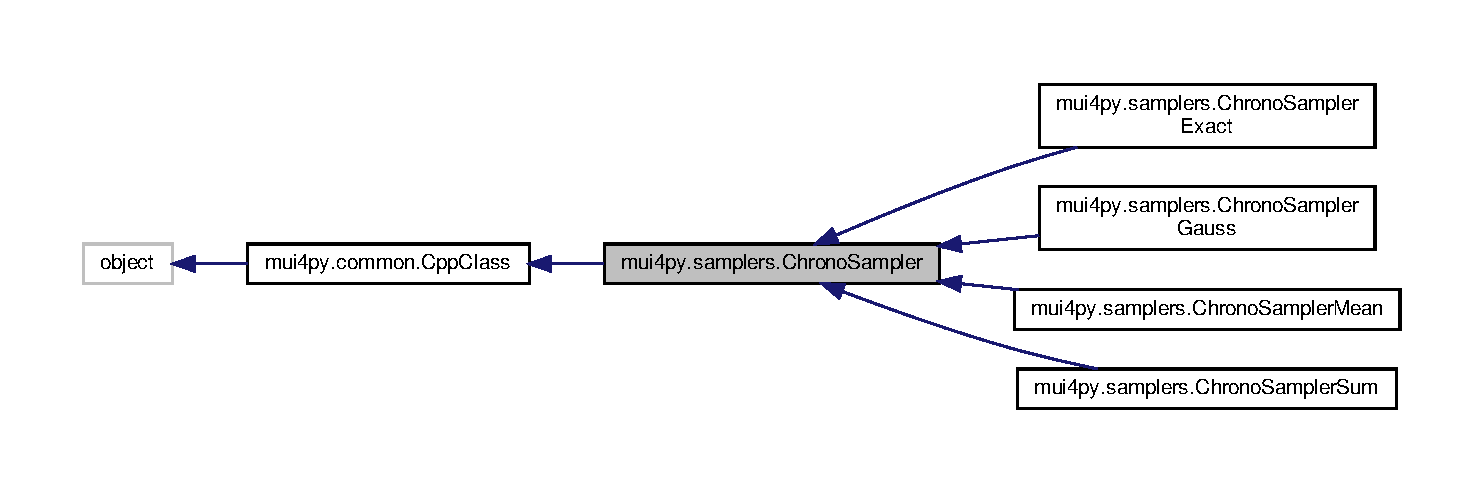
\includegraphics[width=350pt]{classmui4py_1_1samplers_1_1_chrono_sampler__inherit__graph}
\end{center}
\end{figure}


Collaboration diagram for mui4py.\+samplers.\+Chrono\+Sampler\+:
\nopagebreak
\begin{figure}[H]
\begin{center}
\leavevmode
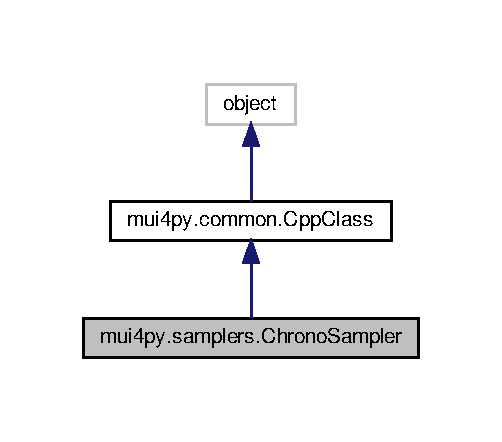
\includegraphics[width=241pt]{classmui4py_1_1samplers_1_1_chrono_sampler__coll__graph}
\end{center}
\end{figure}
\subsection*{Public Member Functions}
\begin{DoxyCompactItemize}
\item 
def \hyperlink{classmui4py_1_1samplers_1_1_chrono_sampler_a2991d523966ed5846bf0210a7e3d5f0e}{\+\_\+\+\_\+init\+\_\+\+\_\+} (self, \hyperlink{classmui4py_1_1common_1_1_cpp_class_a29797823c6e21f22bba24ee7d35ef31d}{args}=(), \hyperlink{classmui4py_1_1common_1_1_cpp_class_af43879f06f07b1abf0d08e30c5ead46f}{kwargs}=\{\})
\end{DoxyCompactItemize}
\subsection*{Additional Inherited Members}


\subsection{Constructor \& Destructor Documentation}
\mbox{\Hypertarget{classmui4py_1_1samplers_1_1_chrono_sampler_a2991d523966ed5846bf0210a7e3d5f0e}\label{classmui4py_1_1samplers_1_1_chrono_sampler_a2991d523966ed5846bf0210a7e3d5f0e}} 
\index{mui4py\+::samplers\+::\+Chrono\+Sampler@{mui4py\+::samplers\+::\+Chrono\+Sampler}!\+\_\+\+\_\+init\+\_\+\+\_\+@{\+\_\+\+\_\+init\+\_\+\+\_\+}}
\index{\+\_\+\+\_\+init\+\_\+\+\_\+@{\+\_\+\+\_\+init\+\_\+\+\_\+}!mui4py\+::samplers\+::\+Chrono\+Sampler@{mui4py\+::samplers\+::\+Chrono\+Sampler}}
\subsubsection{\texorpdfstring{\+\_\+\+\_\+init\+\_\+\+\_\+()}{\_\_init\_\_()}}
{\footnotesize\ttfamily def mui4py.\+samplers.\+Chrono\+Sampler.\+\_\+\+\_\+init\+\_\+\+\_\+ (\begin{DoxyParamCaption}\item[{}]{self,  }\item[{}]{args = {\ttfamily ()},  }\item[{}]{kwargs = {\ttfamily \{\}} }\end{DoxyParamCaption})}



The documentation for this class was generated from the following file\+:\begin{DoxyCompactItemize}
\item 
wrappers/\+Python/mui4py/\hyperlink{samplers_8py}{samplers.\+py}\end{DoxyCompactItemize}

\hypertarget{classmui4py_1_1samplers_1_1_chrono_sampler_exact}{}\section{mui4py.\+samplers.\+Chrono\+Sampler\+Exact Class Reference}
\label{classmui4py_1_1samplers_1_1_chrono_sampler_exact}\index{mui4py.\+samplers.\+Chrono\+Sampler\+Exact@{mui4py.\+samplers.\+Chrono\+Sampler\+Exact}}


Inheritance diagram for mui4py.\+samplers.\+Chrono\+Sampler\+Exact\+:
\nopagebreak
\begin{figure}[H]
\begin{center}
\leavevmode
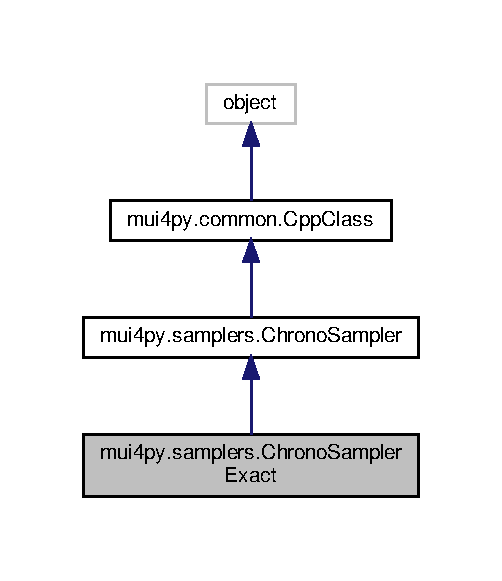
\includegraphics[width=241pt]{classmui4py_1_1samplers_1_1_chrono_sampler_exact__inherit__graph}
\end{center}
\end{figure}


Collaboration diagram for mui4py.\+samplers.\+Chrono\+Sampler\+Exact\+:
\nopagebreak
\begin{figure}[H]
\begin{center}
\leavevmode
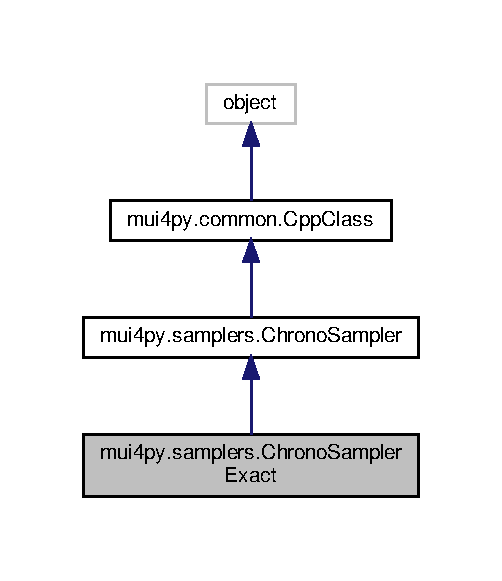
\includegraphics[width=241pt]{classmui4py_1_1samplers_1_1_chrono_sampler_exact__coll__graph}
\end{center}
\end{figure}
\subsection*{Public Member Functions}
\begin{DoxyCompactItemize}
\item 
def \hyperlink{classmui4py_1_1samplers_1_1_chrono_sampler_exact_a501d6cb861ae9e330a15a1a46a894a44}{\+\_\+\+\_\+init\+\_\+\+\_\+} (self, tol=None)
\end{DoxyCompactItemize}
\subsection*{Additional Inherited Members}


\subsection{Constructor \& Destructor Documentation}
\mbox{\Hypertarget{classmui4py_1_1samplers_1_1_chrono_sampler_exact_a501d6cb861ae9e330a15a1a46a894a44}\label{classmui4py_1_1samplers_1_1_chrono_sampler_exact_a501d6cb861ae9e330a15a1a46a894a44}} 
\index{mui4py\+::samplers\+::\+Chrono\+Sampler\+Exact@{mui4py\+::samplers\+::\+Chrono\+Sampler\+Exact}!\+\_\+\+\_\+init\+\_\+\+\_\+@{\+\_\+\+\_\+init\+\_\+\+\_\+}}
\index{\+\_\+\+\_\+init\+\_\+\+\_\+@{\+\_\+\+\_\+init\+\_\+\+\_\+}!mui4py\+::samplers\+::\+Chrono\+Sampler\+Exact@{mui4py\+::samplers\+::\+Chrono\+Sampler\+Exact}}
\subsubsection{\texorpdfstring{\+\_\+\+\_\+init\+\_\+\+\_\+()}{\_\_init\_\_()}}
{\footnotesize\ttfamily def mui4py.\+samplers.\+Chrono\+Sampler\+Exact.\+\_\+\+\_\+init\+\_\+\+\_\+ (\begin{DoxyParamCaption}\item[{}]{self,  }\item[{}]{tol = {\ttfamily None} }\end{DoxyParamCaption})}



The documentation for this class was generated from the following file\+:\begin{DoxyCompactItemize}
\item 
wrappers/\+Python/mui4py/\hyperlink{samplers_8py}{samplers.\+py}\end{DoxyCompactItemize}

\hypertarget{classmui4py_1_1samplers_1_1_chrono_sampler_gauss}{}\section{mui4py.\+samplers.\+Chrono\+Sampler\+Gauss Class Reference}
\label{classmui4py_1_1samplers_1_1_chrono_sampler_gauss}\index{mui4py.\+samplers.\+Chrono\+Sampler\+Gauss@{mui4py.\+samplers.\+Chrono\+Sampler\+Gauss}}


Inheritance diagram for mui4py.\+samplers.\+Chrono\+Sampler\+Gauss\+:
\nopagebreak
\begin{figure}[H]
\begin{center}
\leavevmode
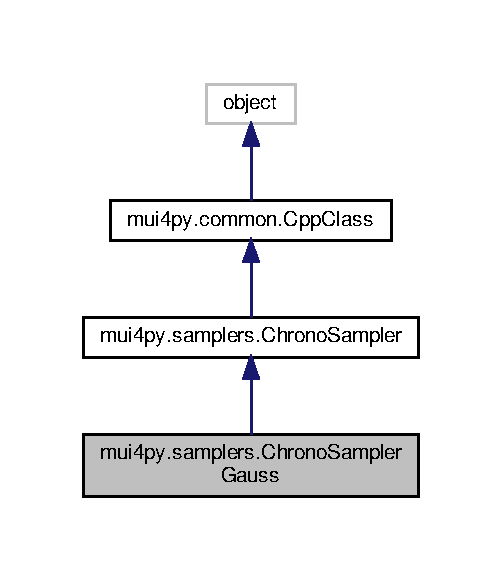
\includegraphics[width=241pt]{classmui4py_1_1samplers_1_1_chrono_sampler_gauss__inherit__graph}
\end{center}
\end{figure}


Collaboration diagram for mui4py.\+samplers.\+Chrono\+Sampler\+Gauss\+:
\nopagebreak
\begin{figure}[H]
\begin{center}
\leavevmode
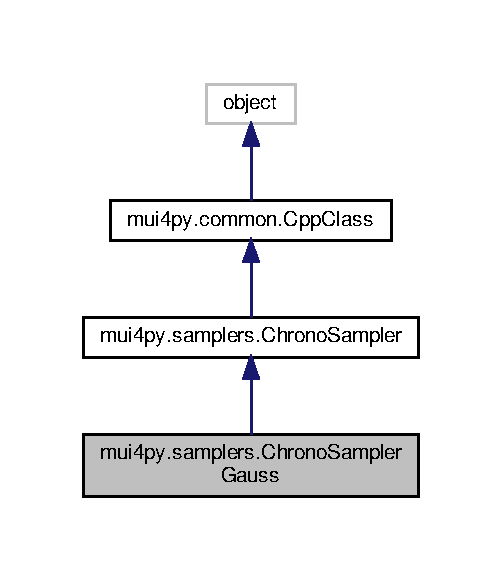
\includegraphics[width=241pt]{classmui4py_1_1samplers_1_1_chrono_sampler_gauss__coll__graph}
\end{center}
\end{figure}
\subsection*{Public Member Functions}
\begin{DoxyCompactItemize}
\item 
def \hyperlink{classmui4py_1_1samplers_1_1_chrono_sampler_gauss_a61feab9954de87869a5248e26c450826}{\+\_\+\+\_\+init\+\_\+\+\_\+} (self, cutoff, sigma)
\end{DoxyCompactItemize}
\subsection*{Additional Inherited Members}


\subsection{Constructor \& Destructor Documentation}
\mbox{\Hypertarget{classmui4py_1_1samplers_1_1_chrono_sampler_gauss_a61feab9954de87869a5248e26c450826}\label{classmui4py_1_1samplers_1_1_chrono_sampler_gauss_a61feab9954de87869a5248e26c450826}} 
\index{mui4py\+::samplers\+::\+Chrono\+Sampler\+Gauss@{mui4py\+::samplers\+::\+Chrono\+Sampler\+Gauss}!\+\_\+\+\_\+init\+\_\+\+\_\+@{\+\_\+\+\_\+init\+\_\+\+\_\+}}
\index{\+\_\+\+\_\+init\+\_\+\+\_\+@{\+\_\+\+\_\+init\+\_\+\+\_\+}!mui4py\+::samplers\+::\+Chrono\+Sampler\+Gauss@{mui4py\+::samplers\+::\+Chrono\+Sampler\+Gauss}}
\subsubsection{\texorpdfstring{\+\_\+\+\_\+init\+\_\+\+\_\+()}{\_\_init\_\_()}}
{\footnotesize\ttfamily def mui4py.\+samplers.\+Chrono\+Sampler\+Gauss.\+\_\+\+\_\+init\+\_\+\+\_\+ (\begin{DoxyParamCaption}\item[{}]{self,  }\item[{}]{cutoff,  }\item[{}]{sigma }\end{DoxyParamCaption})}



The documentation for this class was generated from the following file\+:\begin{DoxyCompactItemize}
\item 
wrappers/\+Python/mui4py/\hyperlink{samplers_8py}{samplers.\+py}\end{DoxyCompactItemize}

\hypertarget{classmui4py_1_1samplers_1_1_chrono_sampler_mean}{}\section{mui4py.\+samplers.\+Chrono\+Sampler\+Mean Class Reference}
\label{classmui4py_1_1samplers_1_1_chrono_sampler_mean}\index{mui4py.\+samplers.\+Chrono\+Sampler\+Mean@{mui4py.\+samplers.\+Chrono\+Sampler\+Mean}}


Inheritance diagram for mui4py.\+samplers.\+Chrono\+Sampler\+Mean\+:
\nopagebreak
\begin{figure}[H]
\begin{center}
\leavevmode
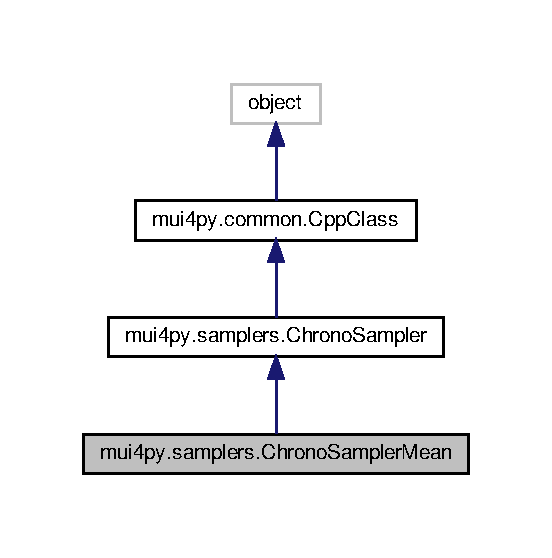
\includegraphics[width=265pt]{classmui4py_1_1samplers_1_1_chrono_sampler_mean__inherit__graph}
\end{center}
\end{figure}


Collaboration diagram for mui4py.\+samplers.\+Chrono\+Sampler\+Mean\+:
\nopagebreak
\begin{figure}[H]
\begin{center}
\leavevmode
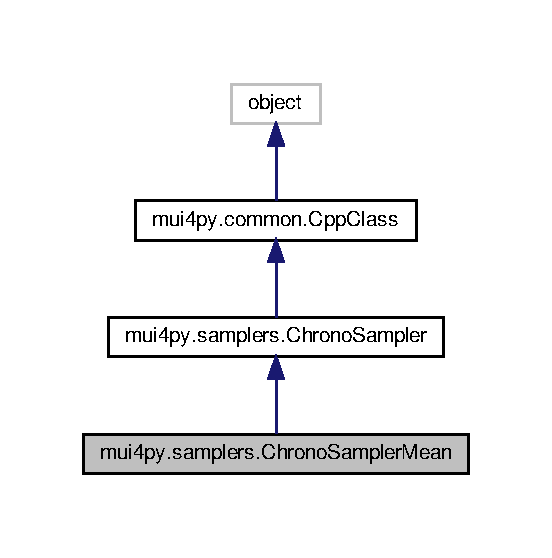
\includegraphics[width=265pt]{classmui4py_1_1samplers_1_1_chrono_sampler_mean__coll__graph}
\end{center}
\end{figure}
\subsection*{Public Member Functions}
\begin{DoxyCompactItemize}
\item 
def \hyperlink{classmui4py_1_1samplers_1_1_chrono_sampler_mean_a27736267f8e88534472d7966c29091bc}{\+\_\+\+\_\+init\+\_\+\+\_\+} (self, newleft=None, newright=None)
\end{DoxyCompactItemize}
\subsection*{Additional Inherited Members}


\subsection{Constructor \& Destructor Documentation}
\mbox{\Hypertarget{classmui4py_1_1samplers_1_1_chrono_sampler_mean_a27736267f8e88534472d7966c29091bc}\label{classmui4py_1_1samplers_1_1_chrono_sampler_mean_a27736267f8e88534472d7966c29091bc}} 
\index{mui4py\+::samplers\+::\+Chrono\+Sampler\+Mean@{mui4py\+::samplers\+::\+Chrono\+Sampler\+Mean}!\+\_\+\+\_\+init\+\_\+\+\_\+@{\+\_\+\+\_\+init\+\_\+\+\_\+}}
\index{\+\_\+\+\_\+init\+\_\+\+\_\+@{\+\_\+\+\_\+init\+\_\+\+\_\+}!mui4py\+::samplers\+::\+Chrono\+Sampler\+Mean@{mui4py\+::samplers\+::\+Chrono\+Sampler\+Mean}}
\subsubsection{\texorpdfstring{\+\_\+\+\_\+init\+\_\+\+\_\+()}{\_\_init\_\_()}}
{\footnotesize\ttfamily def mui4py.\+samplers.\+Chrono\+Sampler\+Mean.\+\_\+\+\_\+init\+\_\+\+\_\+ (\begin{DoxyParamCaption}\item[{}]{self,  }\item[{}]{newleft = {\ttfamily None},  }\item[{}]{newright = {\ttfamily None} }\end{DoxyParamCaption})}



The documentation for this class was generated from the following file\+:\begin{DoxyCompactItemize}
\item 
wrappers/\+Python/mui4py/\hyperlink{samplers_8py}{samplers.\+py}\end{DoxyCompactItemize}

\hypertarget{classmui4py_1_1samplers_1_1_chrono_sampler_sum}{}\section{mui4py.\+samplers.\+Chrono\+Sampler\+Sum Class Reference}
\label{classmui4py_1_1samplers_1_1_chrono_sampler_sum}\index{mui4py.\+samplers.\+Chrono\+Sampler\+Sum@{mui4py.\+samplers.\+Chrono\+Sampler\+Sum}}


Inheritance diagram for mui4py.\+samplers.\+Chrono\+Sampler\+Sum\+:
\nopagebreak
\begin{figure}[H]
\begin{center}
\leavevmode
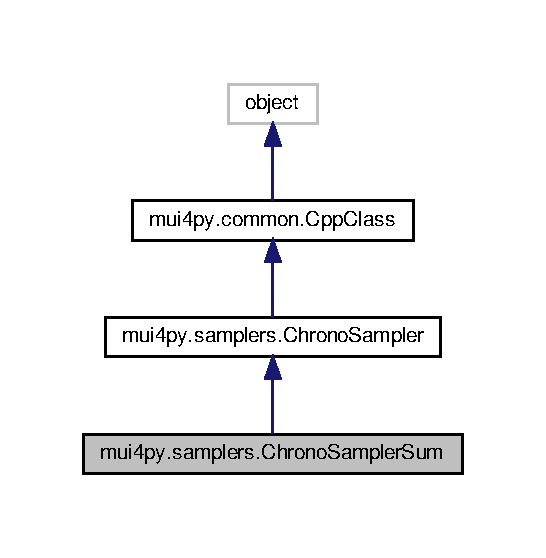
\includegraphics[width=262pt]{classmui4py_1_1samplers_1_1_chrono_sampler_sum__inherit__graph}
\end{center}
\end{figure}


Collaboration diagram for mui4py.\+samplers.\+Chrono\+Sampler\+Sum\+:
\nopagebreak
\begin{figure}[H]
\begin{center}
\leavevmode
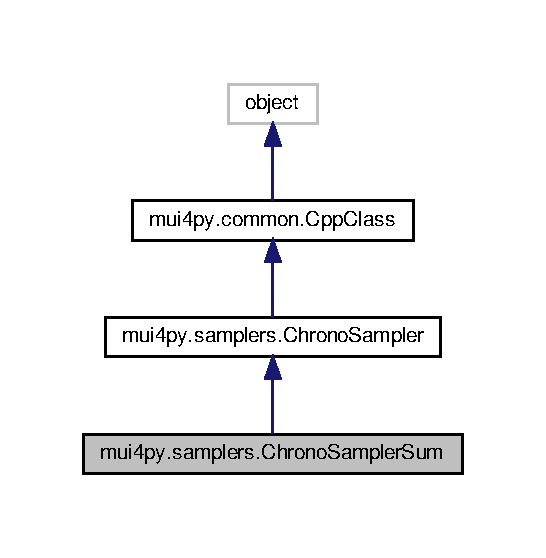
\includegraphics[width=262pt]{classmui4py_1_1samplers_1_1_chrono_sampler_sum__coll__graph}
\end{center}
\end{figure}
\subsection*{Public Member Functions}
\begin{DoxyCompactItemize}
\item 
def \hyperlink{classmui4py_1_1samplers_1_1_chrono_sampler_sum_af32532e7ecd727bb05f3e3390cb8c1f5}{\+\_\+\+\_\+init\+\_\+\+\_\+} (self, newleft=None, newright=None)
\end{DoxyCompactItemize}
\subsection*{Additional Inherited Members}


\subsection{Constructor \& Destructor Documentation}
\mbox{\Hypertarget{classmui4py_1_1samplers_1_1_chrono_sampler_sum_af32532e7ecd727bb05f3e3390cb8c1f5}\label{classmui4py_1_1samplers_1_1_chrono_sampler_sum_af32532e7ecd727bb05f3e3390cb8c1f5}} 
\index{mui4py\+::samplers\+::\+Chrono\+Sampler\+Sum@{mui4py\+::samplers\+::\+Chrono\+Sampler\+Sum}!\+\_\+\+\_\+init\+\_\+\+\_\+@{\+\_\+\+\_\+init\+\_\+\+\_\+}}
\index{\+\_\+\+\_\+init\+\_\+\+\_\+@{\+\_\+\+\_\+init\+\_\+\+\_\+}!mui4py\+::samplers\+::\+Chrono\+Sampler\+Sum@{mui4py\+::samplers\+::\+Chrono\+Sampler\+Sum}}
\subsubsection{\texorpdfstring{\+\_\+\+\_\+init\+\_\+\+\_\+()}{\_\_init\_\_()}}
{\footnotesize\ttfamily def mui4py.\+samplers.\+Chrono\+Sampler\+Sum.\+\_\+\+\_\+init\+\_\+\+\_\+ (\begin{DoxyParamCaption}\item[{}]{self,  }\item[{}]{newleft = {\ttfamily None},  }\item[{}]{newright = {\ttfamily None} }\end{DoxyParamCaption})}



The documentation for this class was generated from the following file\+:\begin{DoxyCompactItemize}
\item 
wrappers/\+Python/mui4py/\hyperlink{samplers_8py}{samplers.\+py}\end{DoxyCompactItemize}

\hypertarget{structmui_1_1comm__factory}{}\section{mui\+:\+:comm\+\_\+factory Struct Reference}
\label{structmui_1_1comm__factory}\index{mui\+::comm\+\_\+factory@{mui\+::comm\+\_\+factory}}


{\ttfamily \#include $<$comm\+\_\+factory.\+h$>$}



Inheritance diagram for mui\+:\+:comm\+\_\+factory\+:
\nopagebreak
\begin{figure}[H]
\begin{center}
\leavevmode
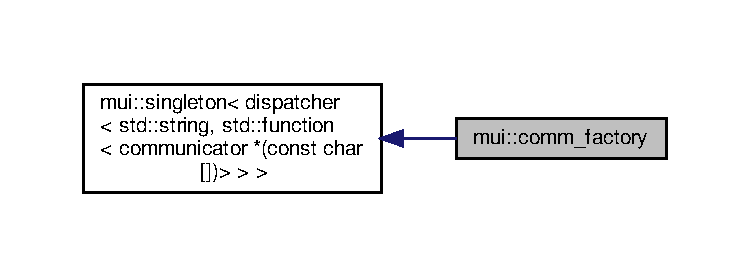
\includegraphics[width=350pt]{structmui_1_1comm__factory__inherit__graph}
\end{center}
\end{figure}


Collaboration diagram for mui\+:\+:comm\+\_\+factory\+:
\nopagebreak
\begin{figure}[H]
\begin{center}
\leavevmode
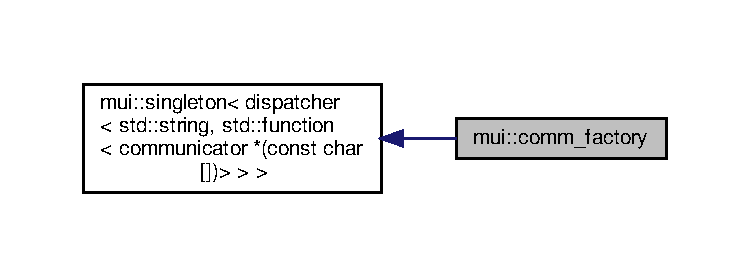
\includegraphics[width=350pt]{structmui_1_1comm__factory__coll__graph}
\end{center}
\end{figure}
\subsection*{Static Public Member Functions}
\begin{DoxyCompactItemize}
\item 
static \hyperlink{classmui_1_1communicator}{communicator} $\ast$ \hyperlink{structmui_1_1comm__factory_adc8cb61ea9f3e4458d3e1c40969218c1}{create\+\_\+comm} (const char U\+RI\mbox{[}$\,$\mbox{]})
\end{DoxyCompactItemize}


\subsection{Member Function Documentation}
\mbox{\Hypertarget{structmui_1_1comm__factory_adc8cb61ea9f3e4458d3e1c40969218c1}\label{structmui_1_1comm__factory_adc8cb61ea9f3e4458d3e1c40969218c1}} 
\index{mui\+::comm\+\_\+factory@{mui\+::comm\+\_\+factory}!create\+\_\+comm@{create\+\_\+comm}}
\index{create\+\_\+comm@{create\+\_\+comm}!mui\+::comm\+\_\+factory@{mui\+::comm\+\_\+factory}}
\subsubsection{\texorpdfstring{create\+\_\+comm()}{create\_comm()}}
{\footnotesize\ttfamily static \hyperlink{classmui_1_1communicator}{communicator}$\ast$ mui\+::comm\+\_\+factory\+::create\+\_\+comm (\begin{DoxyParamCaption}\item[{const char}]{U\+RI\mbox{[}$\,$\mbox{]} }\end{DoxyParamCaption})\hspace{0.3cm}{\ttfamily [inline]}, {\ttfamily [static]}}



The documentation for this struct was generated from the following file\+:\begin{DoxyCompactItemize}
\item 
\hyperlink{comm__factory_8h}{comm\+\_\+factory.\+h}\end{DoxyCompactItemize}

\hypertarget{classmui_1_1comm__fd}{}\section{mui\+:\+:comm\+\_\+fd Class Reference}
\label{classmui_1_1comm__fd}\index{mui\+::comm\+\_\+fd@{mui\+::comm\+\_\+fd}}


{\ttfamily \#include $<$comm\+\_\+tcp.\+h$>$}



Inheritance diagram for mui\+:\+:comm\+\_\+fd\+:
\nopagebreak
\begin{figure}[H]
\begin{center}
\leavevmode
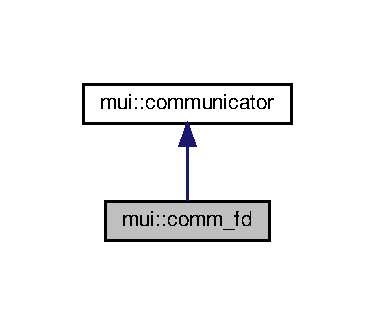
\includegraphics[width=180pt]{classmui_1_1comm__fd__inherit__graph}
\end{center}
\end{figure}


Collaboration diagram for mui\+:\+:comm\+\_\+fd\+:
\nopagebreak
\begin{figure}[H]
\begin{center}
\leavevmode
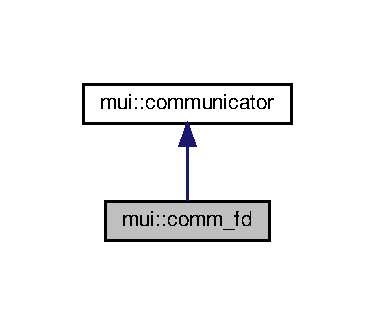
\includegraphics[width=180pt]{classmui_1_1comm__fd__coll__graph}
\end{center}
\end{figure}
\subsection*{Public Member Functions}
\begin{DoxyCompactItemize}
\item 
\hyperlink{classmui_1_1comm__fd_a8b867ed149ab5c043c0ca5fbddd986c0}{comm\+\_\+fd} (int \hyperlink{classmui_1_1comm__fd_ae149073567b5f9997fa3f4bd5fae0336}{local\+\_\+rank}, int \hyperlink{classmui_1_1comm__fd_a9c119bf4de88c8047488750deb2e78ef}{local\+\_\+size}, std\+::vector$<$ \hyperlink{classmui_1_1unique__fd__}{unique\+\_\+fd\+\_\+} $>$ \&\&wfds, std\+::vector$<$ \hyperlink{classmui_1_1unique__fd__}{unique\+\_\+fd\+\_\+} $>$ \&\&rfds)
\item 
\hyperlink{classmui_1_1comm__fd_af584f7becf55e3df14581571ffc71100}{$\sim$comm\+\_\+fd} ()
\item 
int \hyperlink{classmui_1_1comm__fd_ae149073567b5f9997fa3f4bd5fae0336}{local\+\_\+rank} () const
\item 
int \hyperlink{classmui_1_1comm__fd_a9c119bf4de88c8047488750deb2e78ef}{local\+\_\+size} () const
\item 
int \hyperlink{classmui_1_1comm__fd_a6d5e989af8268c87b7c7bcd18a0a9a11}{remote\+\_\+size} () const
\end{DoxyCompactItemize}
\subsection*{Protected Member Functions}
\begin{DoxyCompactItemize}
\item 
void \hyperlink{classmui_1_1comm__fd_a025e0264f0424a2b28f3c14ecde5ba24}{send\+\_\+impl\+\_\+} (\hyperlink{structmui_1_1message}{message} msg, const std\+::vector$<$ bool $>$ \&dest)
\item 
\hyperlink{structmui_1_1message}{message} \hyperlink{classmui_1_1comm__fd_a426bda7ebea0817e24fef87552993756}{recv\+\_\+impl\+\_\+} ()
\end{DoxyCompactItemize}


\subsection{Constructor \& Destructor Documentation}
\mbox{\Hypertarget{classmui_1_1comm__fd_a8b867ed149ab5c043c0ca5fbddd986c0}\label{classmui_1_1comm__fd_a8b867ed149ab5c043c0ca5fbddd986c0}} 
\index{mui\+::comm\+\_\+fd@{mui\+::comm\+\_\+fd}!comm\+\_\+fd@{comm\+\_\+fd}}
\index{comm\+\_\+fd@{comm\+\_\+fd}!mui\+::comm\+\_\+fd@{mui\+::comm\+\_\+fd}}
\subsubsection{\texorpdfstring{comm\+\_\+fd()}{comm\_fd()}}
{\footnotesize\ttfamily mui\+::comm\+\_\+fd\+::comm\+\_\+fd (\begin{DoxyParamCaption}\item[{int}]{local\+\_\+rank,  }\item[{int}]{local\+\_\+size,  }\item[{std\+::vector$<$ \hyperlink{classmui_1_1unique__fd__}{unique\+\_\+fd\+\_\+} $>$ \&\&}]{wfds,  }\item[{std\+::vector$<$ \hyperlink{classmui_1_1unique__fd__}{unique\+\_\+fd\+\_\+} $>$ \&\&}]{rfds }\end{DoxyParamCaption})\hspace{0.3cm}{\ttfamily [inline]}}

\mbox{\Hypertarget{classmui_1_1comm__fd_af584f7becf55e3df14581571ffc71100}\label{classmui_1_1comm__fd_af584f7becf55e3df14581571ffc71100}} 
\index{mui\+::comm\+\_\+fd@{mui\+::comm\+\_\+fd}!````~comm\+\_\+fd@{$\sim$comm\+\_\+fd}}
\index{````~comm\+\_\+fd@{$\sim$comm\+\_\+fd}!mui\+::comm\+\_\+fd@{mui\+::comm\+\_\+fd}}
\subsubsection{\texorpdfstring{$\sim$comm\+\_\+fd()}{~comm\_fd()}}
{\footnotesize\ttfamily mui\+::comm\+\_\+fd\+::$\sim$comm\+\_\+fd (\begin{DoxyParamCaption}{ }\end{DoxyParamCaption})\hspace{0.3cm}{\ttfamily [inline]}}



\subsection{Member Function Documentation}
\mbox{\Hypertarget{classmui_1_1comm__fd_ae149073567b5f9997fa3f4bd5fae0336}\label{classmui_1_1comm__fd_ae149073567b5f9997fa3f4bd5fae0336}} 
\index{mui\+::comm\+\_\+fd@{mui\+::comm\+\_\+fd}!local\+\_\+rank@{local\+\_\+rank}}
\index{local\+\_\+rank@{local\+\_\+rank}!mui\+::comm\+\_\+fd@{mui\+::comm\+\_\+fd}}
\subsubsection{\texorpdfstring{local\+\_\+rank()}{local\_rank()}}
{\footnotesize\ttfamily int mui\+::comm\+\_\+fd\+::local\+\_\+rank (\begin{DoxyParamCaption}{ }\end{DoxyParamCaption}) const\hspace{0.3cm}{\ttfamily [inline]}, {\ttfamily [virtual]}}



Reimplemented from \hyperlink{classmui_1_1communicator_a83311811022225d758dd86866e620466}{mui\+::communicator}.

\mbox{\Hypertarget{classmui_1_1comm__fd_a9c119bf4de88c8047488750deb2e78ef}\label{classmui_1_1comm__fd_a9c119bf4de88c8047488750deb2e78ef}} 
\index{mui\+::comm\+\_\+fd@{mui\+::comm\+\_\+fd}!local\+\_\+size@{local\+\_\+size}}
\index{local\+\_\+size@{local\+\_\+size}!mui\+::comm\+\_\+fd@{mui\+::comm\+\_\+fd}}
\subsubsection{\texorpdfstring{local\+\_\+size()}{local\_size()}}
{\footnotesize\ttfamily int mui\+::comm\+\_\+fd\+::local\+\_\+size (\begin{DoxyParamCaption}{ }\end{DoxyParamCaption}) const\hspace{0.3cm}{\ttfamily [inline]}, {\ttfamily [virtual]}}



Reimplemented from \hyperlink{classmui_1_1communicator_aa98faead0a9f63b8edb8b987477998e1}{mui\+::communicator}.

\mbox{\Hypertarget{classmui_1_1comm__fd_a426bda7ebea0817e24fef87552993756}\label{classmui_1_1comm__fd_a426bda7ebea0817e24fef87552993756}} 
\index{mui\+::comm\+\_\+fd@{mui\+::comm\+\_\+fd}!recv\+\_\+impl\+\_\+@{recv\+\_\+impl\+\_\+}}
\index{recv\+\_\+impl\+\_\+@{recv\+\_\+impl\+\_\+}!mui\+::comm\+\_\+fd@{mui\+::comm\+\_\+fd}}
\subsubsection{\texorpdfstring{recv\+\_\+impl\+\_\+()}{recv\_impl\_()}}
{\footnotesize\ttfamily \hyperlink{structmui_1_1message}{message} mui\+::comm\+\_\+fd\+::recv\+\_\+impl\+\_\+ (\begin{DoxyParamCaption}{ }\end{DoxyParamCaption})\hspace{0.3cm}{\ttfamily [inline]}, {\ttfamily [protected]}, {\ttfamily [virtual]}}



Implements \hyperlink{classmui_1_1communicator_ab52ebf7dd059acdd144493cd76c62c5f}{mui\+::communicator}.

\mbox{\Hypertarget{classmui_1_1comm__fd_a6d5e989af8268c87b7c7bcd18a0a9a11}\label{classmui_1_1comm__fd_a6d5e989af8268c87b7c7bcd18a0a9a11}} 
\index{mui\+::comm\+\_\+fd@{mui\+::comm\+\_\+fd}!remote\+\_\+size@{remote\+\_\+size}}
\index{remote\+\_\+size@{remote\+\_\+size}!mui\+::comm\+\_\+fd@{mui\+::comm\+\_\+fd}}
\subsubsection{\texorpdfstring{remote\+\_\+size()}{remote\_size()}}
{\footnotesize\ttfamily int mui\+::comm\+\_\+fd\+::remote\+\_\+size (\begin{DoxyParamCaption}{ }\end{DoxyParamCaption}) const\hspace{0.3cm}{\ttfamily [inline]}, {\ttfamily [virtual]}}



Reimplemented from \hyperlink{classmui_1_1communicator_a8683d36801b78685ce5a58da2c6a6195}{mui\+::communicator}.

\mbox{\Hypertarget{classmui_1_1comm__fd_a025e0264f0424a2b28f3c14ecde5ba24}\label{classmui_1_1comm__fd_a025e0264f0424a2b28f3c14ecde5ba24}} 
\index{mui\+::comm\+\_\+fd@{mui\+::comm\+\_\+fd}!send\+\_\+impl\+\_\+@{send\+\_\+impl\+\_\+}}
\index{send\+\_\+impl\+\_\+@{send\+\_\+impl\+\_\+}!mui\+::comm\+\_\+fd@{mui\+::comm\+\_\+fd}}
\subsubsection{\texorpdfstring{send\+\_\+impl\+\_\+()}{send\_impl\_()}}
{\footnotesize\ttfamily void mui\+::comm\+\_\+fd\+::send\+\_\+impl\+\_\+ (\begin{DoxyParamCaption}\item[{\hyperlink{structmui_1_1message}{message}}]{msg,  }\item[{const std\+::vector$<$ bool $>$ \&}]{dest }\end{DoxyParamCaption})\hspace{0.3cm}{\ttfamily [inline]}, {\ttfamily [protected]}, {\ttfamily [virtual]}}



Implements \hyperlink{classmui_1_1communicator_a1fccb014ae855d7b7d0fc53f7f22b9aa}{mui\+::communicator}.



The documentation for this class was generated from the following file\+:\begin{DoxyCompactItemize}
\item 
\hyperlink{comm__tcp_8h}{comm\+\_\+tcp.\+h}\end{DoxyCompactItemize}

\hypertarget{classmui_1_1comm__mpi}{}\section{mui\+:\+:comm\+\_\+mpi Class Reference}
\label{classmui_1_1comm__mpi}\index{mui\+::comm\+\_\+mpi@{mui\+::comm\+\_\+mpi}}


{\ttfamily \#include $<$comm\+\_\+mpi.\+h$>$}



Inheritance diagram for mui\+:\+:comm\+\_\+mpi\+:
\nopagebreak
\begin{figure}[H]
\begin{center}
\leavevmode
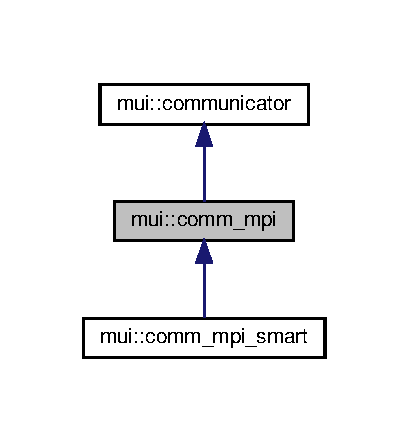
\includegraphics[width=196pt]{classmui_1_1comm__mpi__inherit__graph}
\end{center}
\end{figure}


Collaboration diagram for mui\+:\+:comm\+\_\+mpi\+:
\nopagebreak
\begin{figure}[H]
\begin{center}
\leavevmode
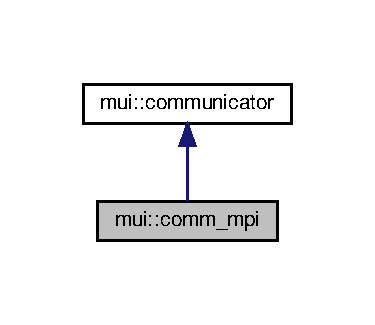
\includegraphics[width=180pt]{classmui_1_1comm__mpi__coll__graph}
\end{center}
\end{figure}
\subsection*{Public Member Functions}
\begin{DoxyCompactItemize}
\item 
\hyperlink{classmui_1_1comm__mpi_a6116417b53d8634c453f3fa2e767c40d}{comm\+\_\+mpi} (const char U\+RI\mbox{[}$\,$\mbox{]}, M\+P\+I\+\_\+\+Comm world)
\item 
virtual \hyperlink{classmui_1_1comm__mpi_a3e55a5ec5ae58ca0f59c7e82afbd391d}{$\sim$comm\+\_\+mpi} ()
\item 
void \hyperlink{classmui_1_1comm__mpi_a4cb3bd6ed04dfea6bcf8ab8136beafaf}{init} (const char U\+RI\mbox{[}$\,$\mbox{]}, M\+P\+I\+\_\+\+Comm world)
\item 
void \hyperlink{classmui_1_1comm__mpi_a7f6419844f743488c069c600ad57d47f}{finalize} ()
\item 
virtual int \hyperlink{classmui_1_1comm__mpi_a580ce0c15f414fe6d80efa74cefa2338}{local\+\_\+size} () const
\item 
virtual int \hyperlink{classmui_1_1comm__mpi_ab0cf03ad7dbe099e0859a920f2711709}{local\+\_\+rank} () const
\item 
virtual int \hyperlink{classmui_1_1comm__mpi_abbf8ab973f51af297cc7ecf145f6cd84}{remote\+\_\+size} () const
\item 
virtual int \hyperlink{classmui_1_1comm__mpi_ad96c274b259a5aa4a4c18882dace97a7}{global\+\_\+size} () const
\item 
virtual int \hyperlink{classmui_1_1comm__mpi_ad2413502326fd78d453978abf96ad9de}{global\+\_\+rank} () const
\end{DoxyCompactItemize}
\subsection*{Protected Attributes}
\begin{DoxyCompactItemize}
\item 
M\+P\+I\+\_\+\+Comm \hyperlink{classmui_1_1comm__mpi_a54674e884ecca1e64d8ccdc6798c589e}{domain\+\_\+local\+\_\+}
\item 
M\+P\+I\+\_\+\+Comm \hyperlink{classmui_1_1comm__mpi_a414000a7c43087ca378d85c45dbaebc9}{domain\+\_\+remote\+\_\+}
\item 
int \hyperlink{classmui_1_1comm__mpi_ae9f2f6f5e3ea067feb9534dd2b5f0b40}{local\+\_\+size\+\_\+}
\item 
int \hyperlink{classmui_1_1comm__mpi_a143de5dac5348ae4e3929ed3a3d8459d}{local\+\_\+rank\+\_\+}
\item 
int \hyperlink{classmui_1_1comm__mpi_a7d9f55e3220ea9b5975cccc06645abf7}{remote\+\_\+size\+\_\+}
\item 
int \hyperlink{classmui_1_1comm__mpi_a69f9224cba14db3d63ef24a0e9cd1693}{global\+\_\+size\+\_\+}
\item 
int \hyperlink{classmui_1_1comm__mpi_a43678dec5d23ec36d1833e5c9c1b1f94}{global\+\_\+rank\+\_\+}
\end{DoxyCompactItemize}
\subsection*{Additional Inherited Members}


\subsection{Constructor \& Destructor Documentation}
\mbox{\Hypertarget{classmui_1_1comm__mpi_a6116417b53d8634c453f3fa2e767c40d}\label{classmui_1_1comm__mpi_a6116417b53d8634c453f3fa2e767c40d}} 
\index{mui\+::comm\+\_\+mpi@{mui\+::comm\+\_\+mpi}!comm\+\_\+mpi@{comm\+\_\+mpi}}
\index{comm\+\_\+mpi@{comm\+\_\+mpi}!mui\+::comm\+\_\+mpi@{mui\+::comm\+\_\+mpi}}
\subsubsection{\texorpdfstring{comm\+\_\+mpi()}{comm\_mpi()}}
{\footnotesize\ttfamily mui\+::comm\+\_\+mpi\+::comm\+\_\+mpi (\begin{DoxyParamCaption}\item[{const char}]{U\+RI\mbox{[}$\,$\mbox{]},  }\item[{M\+P\+I\+\_\+\+Comm}]{world }\end{DoxyParamCaption})\hspace{0.3cm}{\ttfamily [inline]}}

\mbox{\Hypertarget{classmui_1_1comm__mpi_a3e55a5ec5ae58ca0f59c7e82afbd391d}\label{classmui_1_1comm__mpi_a3e55a5ec5ae58ca0f59c7e82afbd391d}} 
\index{mui\+::comm\+\_\+mpi@{mui\+::comm\+\_\+mpi}!````~comm\+\_\+mpi@{$\sim$comm\+\_\+mpi}}
\index{````~comm\+\_\+mpi@{$\sim$comm\+\_\+mpi}!mui\+::comm\+\_\+mpi@{mui\+::comm\+\_\+mpi}}
\subsubsection{\texorpdfstring{$\sim$comm\+\_\+mpi()}{~comm\_mpi()}}
{\footnotesize\ttfamily virtual mui\+::comm\+\_\+mpi\+::$\sim$comm\+\_\+mpi (\begin{DoxyParamCaption}{ }\end{DoxyParamCaption})\hspace{0.3cm}{\ttfamily [inline]}, {\ttfamily [virtual]}}



\subsection{Member Function Documentation}
\mbox{\Hypertarget{classmui_1_1comm__mpi_a7f6419844f743488c069c600ad57d47f}\label{classmui_1_1comm__mpi_a7f6419844f743488c069c600ad57d47f}} 
\index{mui\+::comm\+\_\+mpi@{mui\+::comm\+\_\+mpi}!finalize@{finalize}}
\index{finalize@{finalize}!mui\+::comm\+\_\+mpi@{mui\+::comm\+\_\+mpi}}
\subsubsection{\texorpdfstring{finalize()}{finalize()}}
{\footnotesize\ttfamily void mui\+::comm\+\_\+mpi\+::finalize (\begin{DoxyParamCaption}{ }\end{DoxyParamCaption})\hspace{0.3cm}{\ttfamily [inline]}}

\mbox{\Hypertarget{classmui_1_1comm__mpi_ad2413502326fd78d453978abf96ad9de}\label{classmui_1_1comm__mpi_ad2413502326fd78d453978abf96ad9de}} 
\index{mui\+::comm\+\_\+mpi@{mui\+::comm\+\_\+mpi}!global\+\_\+rank@{global\+\_\+rank}}
\index{global\+\_\+rank@{global\+\_\+rank}!mui\+::comm\+\_\+mpi@{mui\+::comm\+\_\+mpi}}
\subsubsection{\texorpdfstring{global\+\_\+rank()}{global\_rank()}}
{\footnotesize\ttfamily virtual int mui\+::comm\+\_\+mpi\+::global\+\_\+rank (\begin{DoxyParamCaption}{ }\end{DoxyParamCaption}) const\hspace{0.3cm}{\ttfamily [inline]}, {\ttfamily [virtual]}}

\mbox{\Hypertarget{classmui_1_1comm__mpi_ad96c274b259a5aa4a4c18882dace97a7}\label{classmui_1_1comm__mpi_ad96c274b259a5aa4a4c18882dace97a7}} 
\index{mui\+::comm\+\_\+mpi@{mui\+::comm\+\_\+mpi}!global\+\_\+size@{global\+\_\+size}}
\index{global\+\_\+size@{global\+\_\+size}!mui\+::comm\+\_\+mpi@{mui\+::comm\+\_\+mpi}}
\subsubsection{\texorpdfstring{global\+\_\+size()}{global\_size()}}
{\footnotesize\ttfamily virtual int mui\+::comm\+\_\+mpi\+::global\+\_\+size (\begin{DoxyParamCaption}{ }\end{DoxyParamCaption}) const\hspace{0.3cm}{\ttfamily [inline]}, {\ttfamily [virtual]}}

\mbox{\Hypertarget{classmui_1_1comm__mpi_a4cb3bd6ed04dfea6bcf8ab8136beafaf}\label{classmui_1_1comm__mpi_a4cb3bd6ed04dfea6bcf8ab8136beafaf}} 
\index{mui\+::comm\+\_\+mpi@{mui\+::comm\+\_\+mpi}!init@{init}}
\index{init@{init}!mui\+::comm\+\_\+mpi@{mui\+::comm\+\_\+mpi}}
\subsubsection{\texorpdfstring{init()}{init()}}
{\footnotesize\ttfamily void mui\+::comm\+\_\+mpi\+::init (\begin{DoxyParamCaption}\item[{const char}]{U\+RI\mbox{[}$\,$\mbox{]},  }\item[{M\+P\+I\+\_\+\+Comm}]{world }\end{DoxyParamCaption})\hspace{0.3cm}{\ttfamily [inline]}}

\mbox{\Hypertarget{classmui_1_1comm__mpi_ab0cf03ad7dbe099e0859a920f2711709}\label{classmui_1_1comm__mpi_ab0cf03ad7dbe099e0859a920f2711709}} 
\index{mui\+::comm\+\_\+mpi@{mui\+::comm\+\_\+mpi}!local\+\_\+rank@{local\+\_\+rank}}
\index{local\+\_\+rank@{local\+\_\+rank}!mui\+::comm\+\_\+mpi@{mui\+::comm\+\_\+mpi}}
\subsubsection{\texorpdfstring{local\+\_\+rank()}{local\_rank()}}
{\footnotesize\ttfamily virtual int mui\+::comm\+\_\+mpi\+::local\+\_\+rank (\begin{DoxyParamCaption}{ }\end{DoxyParamCaption}) const\hspace{0.3cm}{\ttfamily [inline]}, {\ttfamily [virtual]}}



Reimplemented from \hyperlink{classmui_1_1communicator_a83311811022225d758dd86866e620466}{mui\+::communicator}.

\mbox{\Hypertarget{classmui_1_1comm__mpi_a580ce0c15f414fe6d80efa74cefa2338}\label{classmui_1_1comm__mpi_a580ce0c15f414fe6d80efa74cefa2338}} 
\index{mui\+::comm\+\_\+mpi@{mui\+::comm\+\_\+mpi}!local\+\_\+size@{local\+\_\+size}}
\index{local\+\_\+size@{local\+\_\+size}!mui\+::comm\+\_\+mpi@{mui\+::comm\+\_\+mpi}}
\subsubsection{\texorpdfstring{local\+\_\+size()}{local\_size()}}
{\footnotesize\ttfamily virtual int mui\+::comm\+\_\+mpi\+::local\+\_\+size (\begin{DoxyParamCaption}{ }\end{DoxyParamCaption}) const\hspace{0.3cm}{\ttfamily [inline]}, {\ttfamily [virtual]}}



Reimplemented from \hyperlink{classmui_1_1communicator_aa98faead0a9f63b8edb8b987477998e1}{mui\+::communicator}.

\mbox{\Hypertarget{classmui_1_1comm__mpi_abbf8ab973f51af297cc7ecf145f6cd84}\label{classmui_1_1comm__mpi_abbf8ab973f51af297cc7ecf145f6cd84}} 
\index{mui\+::comm\+\_\+mpi@{mui\+::comm\+\_\+mpi}!remote\+\_\+size@{remote\+\_\+size}}
\index{remote\+\_\+size@{remote\+\_\+size}!mui\+::comm\+\_\+mpi@{mui\+::comm\+\_\+mpi}}
\subsubsection{\texorpdfstring{remote\+\_\+size()}{remote\_size()}}
{\footnotesize\ttfamily virtual int mui\+::comm\+\_\+mpi\+::remote\+\_\+size (\begin{DoxyParamCaption}{ }\end{DoxyParamCaption}) const\hspace{0.3cm}{\ttfamily [inline]}, {\ttfamily [virtual]}}



Reimplemented from \hyperlink{classmui_1_1communicator_a8683d36801b78685ce5a58da2c6a6195}{mui\+::communicator}.



\subsection{Member Data Documentation}
\mbox{\Hypertarget{classmui_1_1comm__mpi_a54674e884ecca1e64d8ccdc6798c589e}\label{classmui_1_1comm__mpi_a54674e884ecca1e64d8ccdc6798c589e}} 
\index{mui\+::comm\+\_\+mpi@{mui\+::comm\+\_\+mpi}!domain\+\_\+local\+\_\+@{domain\+\_\+local\+\_\+}}
\index{domain\+\_\+local\+\_\+@{domain\+\_\+local\+\_\+}!mui\+::comm\+\_\+mpi@{mui\+::comm\+\_\+mpi}}
\subsubsection{\texorpdfstring{domain\+\_\+local\+\_\+}{domain\_local\_}}
{\footnotesize\ttfamily M\+P\+I\+\_\+\+Comm mui\+::comm\+\_\+mpi\+::domain\+\_\+local\+\_\+\hspace{0.3cm}{\ttfamily [protected]}}

\mbox{\Hypertarget{classmui_1_1comm__mpi_a414000a7c43087ca378d85c45dbaebc9}\label{classmui_1_1comm__mpi_a414000a7c43087ca378d85c45dbaebc9}} 
\index{mui\+::comm\+\_\+mpi@{mui\+::comm\+\_\+mpi}!domain\+\_\+remote\+\_\+@{domain\+\_\+remote\+\_\+}}
\index{domain\+\_\+remote\+\_\+@{domain\+\_\+remote\+\_\+}!mui\+::comm\+\_\+mpi@{mui\+::comm\+\_\+mpi}}
\subsubsection{\texorpdfstring{domain\+\_\+remote\+\_\+}{domain\_remote\_}}
{\footnotesize\ttfamily M\+P\+I\+\_\+\+Comm mui\+::comm\+\_\+mpi\+::domain\+\_\+remote\+\_\+\hspace{0.3cm}{\ttfamily [protected]}}

\mbox{\Hypertarget{classmui_1_1comm__mpi_a43678dec5d23ec36d1833e5c9c1b1f94}\label{classmui_1_1comm__mpi_a43678dec5d23ec36d1833e5c9c1b1f94}} 
\index{mui\+::comm\+\_\+mpi@{mui\+::comm\+\_\+mpi}!global\+\_\+rank\+\_\+@{global\+\_\+rank\+\_\+}}
\index{global\+\_\+rank\+\_\+@{global\+\_\+rank\+\_\+}!mui\+::comm\+\_\+mpi@{mui\+::comm\+\_\+mpi}}
\subsubsection{\texorpdfstring{global\+\_\+rank\+\_\+}{global\_rank\_}}
{\footnotesize\ttfamily int mui\+::comm\+\_\+mpi\+::global\+\_\+rank\+\_\+\hspace{0.3cm}{\ttfamily [protected]}}

\mbox{\Hypertarget{classmui_1_1comm__mpi_a69f9224cba14db3d63ef24a0e9cd1693}\label{classmui_1_1comm__mpi_a69f9224cba14db3d63ef24a0e9cd1693}} 
\index{mui\+::comm\+\_\+mpi@{mui\+::comm\+\_\+mpi}!global\+\_\+size\+\_\+@{global\+\_\+size\+\_\+}}
\index{global\+\_\+size\+\_\+@{global\+\_\+size\+\_\+}!mui\+::comm\+\_\+mpi@{mui\+::comm\+\_\+mpi}}
\subsubsection{\texorpdfstring{global\+\_\+size\+\_\+}{global\_size\_}}
{\footnotesize\ttfamily int mui\+::comm\+\_\+mpi\+::global\+\_\+size\+\_\+\hspace{0.3cm}{\ttfamily [protected]}}

\mbox{\Hypertarget{classmui_1_1comm__mpi_a143de5dac5348ae4e3929ed3a3d8459d}\label{classmui_1_1comm__mpi_a143de5dac5348ae4e3929ed3a3d8459d}} 
\index{mui\+::comm\+\_\+mpi@{mui\+::comm\+\_\+mpi}!local\+\_\+rank\+\_\+@{local\+\_\+rank\+\_\+}}
\index{local\+\_\+rank\+\_\+@{local\+\_\+rank\+\_\+}!mui\+::comm\+\_\+mpi@{mui\+::comm\+\_\+mpi}}
\subsubsection{\texorpdfstring{local\+\_\+rank\+\_\+}{local\_rank\_}}
{\footnotesize\ttfamily int mui\+::comm\+\_\+mpi\+::local\+\_\+rank\+\_\+\hspace{0.3cm}{\ttfamily [protected]}}

\mbox{\Hypertarget{classmui_1_1comm__mpi_ae9f2f6f5e3ea067feb9534dd2b5f0b40}\label{classmui_1_1comm__mpi_ae9f2f6f5e3ea067feb9534dd2b5f0b40}} 
\index{mui\+::comm\+\_\+mpi@{mui\+::comm\+\_\+mpi}!local\+\_\+size\+\_\+@{local\+\_\+size\+\_\+}}
\index{local\+\_\+size\+\_\+@{local\+\_\+size\+\_\+}!mui\+::comm\+\_\+mpi@{mui\+::comm\+\_\+mpi}}
\subsubsection{\texorpdfstring{local\+\_\+size\+\_\+}{local\_size\_}}
{\footnotesize\ttfamily int mui\+::comm\+\_\+mpi\+::local\+\_\+size\+\_\+\hspace{0.3cm}{\ttfamily [protected]}}

\mbox{\Hypertarget{classmui_1_1comm__mpi_a7d9f55e3220ea9b5975cccc06645abf7}\label{classmui_1_1comm__mpi_a7d9f55e3220ea9b5975cccc06645abf7}} 
\index{mui\+::comm\+\_\+mpi@{mui\+::comm\+\_\+mpi}!remote\+\_\+size\+\_\+@{remote\+\_\+size\+\_\+}}
\index{remote\+\_\+size\+\_\+@{remote\+\_\+size\+\_\+}!mui\+::comm\+\_\+mpi@{mui\+::comm\+\_\+mpi}}
\subsubsection{\texorpdfstring{remote\+\_\+size\+\_\+}{remote\_size\_}}
{\footnotesize\ttfamily int mui\+::comm\+\_\+mpi\+::remote\+\_\+size\+\_\+\hspace{0.3cm}{\ttfamily [protected]}}



The documentation for this class was generated from the following file\+:\begin{DoxyCompactItemize}
\item 
\hyperlink{comm__mpi_8h}{comm\+\_\+mpi.\+h}\end{DoxyCompactItemize}

\hypertarget{classmui_1_1comm__mpi__smart}{}\section{mui\+:\+:comm\+\_\+mpi\+\_\+smart Class Reference}
\label{classmui_1_1comm__mpi__smart}\index{mui\+::comm\+\_\+mpi\+\_\+smart@{mui\+::comm\+\_\+mpi\+\_\+smart}}


{\ttfamily \#include $<$comm\+\_\+mpi\+\_\+smart.\+h$>$}



Inheritance diagram for mui\+:\+:comm\+\_\+mpi\+\_\+smart\+:
\nopagebreak
\begin{figure}[H]
\begin{center}
\leavevmode
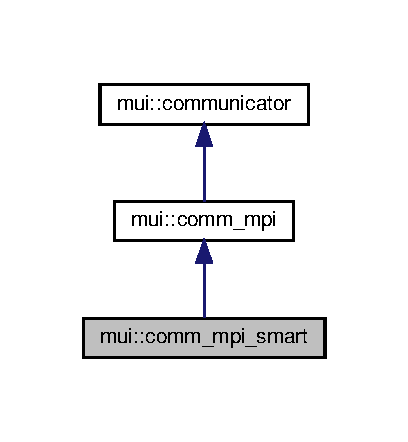
\includegraphics[width=196pt]{classmui_1_1comm__mpi__smart__inherit__graph}
\end{center}
\end{figure}


Collaboration diagram for mui\+:\+:comm\+\_\+mpi\+\_\+smart\+:
\nopagebreak
\begin{figure}[H]
\begin{center}
\leavevmode
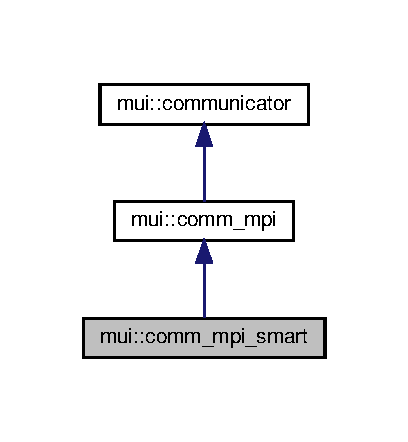
\includegraphics[width=196pt]{classmui_1_1comm__mpi__smart__coll__graph}
\end{center}
\end{figure}
\subsection*{Public Member Functions}
\begin{DoxyCompactItemize}
\item 
\hyperlink{classmui_1_1comm__mpi__smart_a4affdf87d8bfc20fd04c6c21ad1626bf}{comm\+\_\+mpi\+\_\+smart} (const char U\+RI\mbox{[}$\,$\mbox{]}, M\+P\+I\+\_\+\+Comm world=M\+P\+I\+\_\+\+C\+O\+M\+M\+\_\+\+W\+O\+R\+LD)
\item 
virtual \hyperlink{classmui_1_1comm__mpi__smart_aff9965e2368beade94d6a33965a6316d}{$\sim$comm\+\_\+mpi\+\_\+smart} ()
\end{DoxyCompactItemize}
\subsection*{Additional Inherited Members}


\subsection{Constructor \& Destructor Documentation}
\mbox{\Hypertarget{classmui_1_1comm__mpi__smart_a4affdf87d8bfc20fd04c6c21ad1626bf}\label{classmui_1_1comm__mpi__smart_a4affdf87d8bfc20fd04c6c21ad1626bf}} 
\index{mui\+::comm\+\_\+mpi\+\_\+smart@{mui\+::comm\+\_\+mpi\+\_\+smart}!comm\+\_\+mpi\+\_\+smart@{comm\+\_\+mpi\+\_\+smart}}
\index{comm\+\_\+mpi\+\_\+smart@{comm\+\_\+mpi\+\_\+smart}!mui\+::comm\+\_\+mpi\+\_\+smart@{mui\+::comm\+\_\+mpi\+\_\+smart}}
\subsubsection{\texorpdfstring{comm\+\_\+mpi\+\_\+smart()}{comm\_mpi\_smart()}}
{\footnotesize\ttfamily mui\+::comm\+\_\+mpi\+\_\+smart\+::comm\+\_\+mpi\+\_\+smart (\begin{DoxyParamCaption}\item[{const char}]{U\+RI\mbox{[}$\,$\mbox{]},  }\item[{M\+P\+I\+\_\+\+Comm}]{world = {\ttfamily MPI\+\_\+COMM\+\_\+WORLD} }\end{DoxyParamCaption})\hspace{0.3cm}{\ttfamily [inline]}}

\mbox{\Hypertarget{classmui_1_1comm__mpi__smart_aff9965e2368beade94d6a33965a6316d}\label{classmui_1_1comm__mpi__smart_aff9965e2368beade94d6a33965a6316d}} 
\index{mui\+::comm\+\_\+mpi\+\_\+smart@{mui\+::comm\+\_\+mpi\+\_\+smart}!````~comm\+\_\+mpi\+\_\+smart@{$\sim$comm\+\_\+mpi\+\_\+smart}}
\index{````~comm\+\_\+mpi\+\_\+smart@{$\sim$comm\+\_\+mpi\+\_\+smart}!mui\+::comm\+\_\+mpi\+\_\+smart@{mui\+::comm\+\_\+mpi\+\_\+smart}}
\subsubsection{\texorpdfstring{$\sim$comm\+\_\+mpi\+\_\+smart()}{~comm\_mpi\_smart()}}
{\footnotesize\ttfamily virtual mui\+::comm\+\_\+mpi\+\_\+smart\+::$\sim$comm\+\_\+mpi\+\_\+smart (\begin{DoxyParamCaption}{ }\end{DoxyParamCaption})\hspace{0.3cm}{\ttfamily [inline]}, {\ttfamily [virtual]}}



The documentation for this class was generated from the following file\+:\begin{DoxyCompactItemize}
\item 
\hyperlink{comm__mpi__smart_8h}{comm\+\_\+mpi\+\_\+smart.\+h}\end{DoxyCompactItemize}

\hypertarget{classmui_1_1communicator}{}\section{mui\+:\+:communicator Class Reference}
\label{classmui_1_1communicator}\index{mui\+::communicator@{mui\+::communicator}}


{\ttfamily \#include $<$comm.\+h$>$}



Inheritance diagram for mui\+:\+:communicator\+:
\nopagebreak
\begin{figure}[H]
\begin{center}
\leavevmode
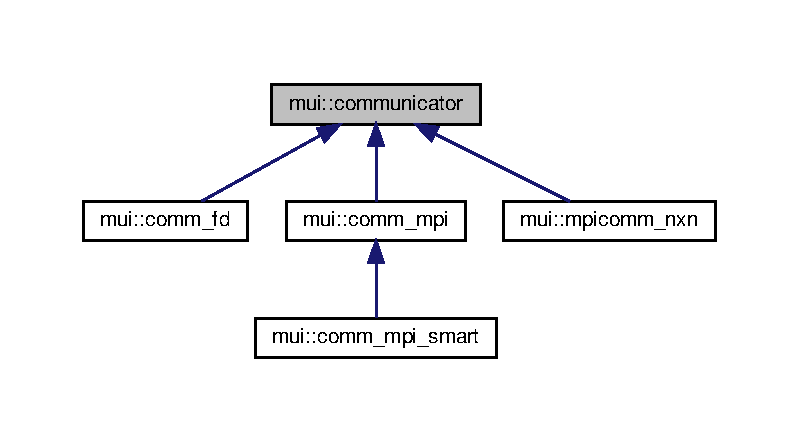
\includegraphics[width=350pt]{classmui_1_1communicator__inherit__graph}
\end{center}
\end{figure}
\subsection*{Public Member Functions}
\begin{DoxyCompactItemize}
\item 
\hyperlink{classmui_1_1communicator_a115082ed8993d41bb492e985041e86e4}{communicator} ()
\item 
virtual \hyperlink{classmui_1_1communicator_aa7f8c2ace12e778f7f710a3058953c44}{$\sim$communicator} ()
\item 
virtual int \hyperlink{classmui_1_1communicator_a83311811022225d758dd86866e620466}{local\+\_\+rank} () const
\item 
virtual int \hyperlink{classmui_1_1communicator_aa98faead0a9f63b8edb8b987477998e1}{local\+\_\+size} () const
\item 
virtual int \hyperlink{classmui_1_1communicator_a8683d36801b78685ce5a58da2c6a6195}{remote\+\_\+size} () const
\item 
void \hyperlink{classmui_1_1communicator_ae81f0d5aedaad66cad99ff0d8258e72c}{send} (\hyperlink{structmui_1_1message}{message} msg, const std\+::vector$<$ bool $>$ \&is\+\_\+sending)
\item 
void \hyperlink{classmui_1_1communicator_ae6e96be2a9ef6ebbd1ead1add1921181}{send} (\hyperlink{structmui_1_1message}{message} msg)
\item 
\hyperlink{structmui_1_1message}{message} \hyperlink{classmui_1_1communicator_a1c2f180ccf56e7121333ccbeb1c70041}{recv} ()
\end{DoxyCompactItemize}
\subsection*{Protected Member Functions}
\begin{DoxyCompactItemize}
\item 
virtual void \hyperlink{classmui_1_1communicator_a1fccb014ae855d7b7d0fc53f7f22b9aa}{send\+\_\+impl\+\_\+} (\hyperlink{structmui_1_1message}{message} msg, const std\+::vector$<$ bool $>$ \&is\+\_\+sending)=0
\item 
virtual \hyperlink{structmui_1_1message}{message} \hyperlink{classmui_1_1communicator_ab52ebf7dd059acdd144493cd76c62c5f}{recv\+\_\+impl\+\_\+} ()=0
\end{DoxyCompactItemize}


\subsection{Constructor \& Destructor Documentation}
\mbox{\Hypertarget{classmui_1_1communicator_a115082ed8993d41bb492e985041e86e4}\label{classmui_1_1communicator_a115082ed8993d41bb492e985041e86e4}} 
\index{mui\+::communicator@{mui\+::communicator}!communicator@{communicator}}
\index{communicator@{communicator}!mui\+::communicator@{mui\+::communicator}}
\subsubsection{\texorpdfstring{communicator()}{communicator()}}
{\footnotesize\ttfamily mui\+::communicator\+::communicator (\begin{DoxyParamCaption}{ }\end{DoxyParamCaption})\hspace{0.3cm}{\ttfamily [inline]}}

\mbox{\Hypertarget{classmui_1_1communicator_aa7f8c2ace12e778f7f710a3058953c44}\label{classmui_1_1communicator_aa7f8c2ace12e778f7f710a3058953c44}} 
\index{mui\+::communicator@{mui\+::communicator}!````~communicator@{$\sim$communicator}}
\index{````~communicator@{$\sim$communicator}!mui\+::communicator@{mui\+::communicator}}
\subsubsection{\texorpdfstring{$\sim$communicator()}{~communicator()}}
{\footnotesize\ttfamily virtual mui\+::communicator\+::$\sim$communicator (\begin{DoxyParamCaption}{ }\end{DoxyParamCaption})\hspace{0.3cm}{\ttfamily [inline]}, {\ttfamily [virtual]}}



\subsection{Member Function Documentation}
\mbox{\Hypertarget{classmui_1_1communicator_a83311811022225d758dd86866e620466}\label{classmui_1_1communicator_a83311811022225d758dd86866e620466}} 
\index{mui\+::communicator@{mui\+::communicator}!local\+\_\+rank@{local\+\_\+rank}}
\index{local\+\_\+rank@{local\+\_\+rank}!mui\+::communicator@{mui\+::communicator}}
\subsubsection{\texorpdfstring{local\+\_\+rank()}{local\_rank()}}
{\footnotesize\ttfamily virtual int mui\+::communicator\+::local\+\_\+rank (\begin{DoxyParamCaption}{ }\end{DoxyParamCaption}) const\hspace{0.3cm}{\ttfamily [inline]}, {\ttfamily [virtual]}}



Reimplemented in \hyperlink{classmui_1_1comm__fd_ae149073567b5f9997fa3f4bd5fae0336}{mui\+::comm\+\_\+fd}, and \hyperlink{classmui_1_1comm__mpi_ab0cf03ad7dbe099e0859a920f2711709}{mui\+::comm\+\_\+mpi}.

\mbox{\Hypertarget{classmui_1_1communicator_aa98faead0a9f63b8edb8b987477998e1}\label{classmui_1_1communicator_aa98faead0a9f63b8edb8b987477998e1}} 
\index{mui\+::communicator@{mui\+::communicator}!local\+\_\+size@{local\+\_\+size}}
\index{local\+\_\+size@{local\+\_\+size}!mui\+::communicator@{mui\+::communicator}}
\subsubsection{\texorpdfstring{local\+\_\+size()}{local\_size()}}
{\footnotesize\ttfamily virtual int mui\+::communicator\+::local\+\_\+size (\begin{DoxyParamCaption}{ }\end{DoxyParamCaption}) const\hspace{0.3cm}{\ttfamily [inline]}, {\ttfamily [virtual]}}



Reimplemented in \hyperlink{classmui_1_1comm__fd_a9c119bf4de88c8047488750deb2e78ef}{mui\+::comm\+\_\+fd}, \hyperlink{classmui_1_1comm__mpi_a580ce0c15f414fe6d80efa74cefa2338}{mui\+::comm\+\_\+mpi}, and \hyperlink{classmui_1_1mpicomm__nxn_aa30777638394ee6f17851f06c7793454}{mui\+::mpicomm\+\_\+nxn}.

\mbox{\Hypertarget{classmui_1_1communicator_a1c2f180ccf56e7121333ccbeb1c70041}\label{classmui_1_1communicator_a1c2f180ccf56e7121333ccbeb1c70041}} 
\index{mui\+::communicator@{mui\+::communicator}!recv@{recv}}
\index{recv@{recv}!mui\+::communicator@{mui\+::communicator}}
\subsubsection{\texorpdfstring{recv()}{recv()}}
{\footnotesize\ttfamily \hyperlink{structmui_1_1message}{message} mui\+::communicator\+::recv (\begin{DoxyParamCaption}{ }\end{DoxyParamCaption})\hspace{0.3cm}{\ttfamily [inline]}}

\mbox{\Hypertarget{classmui_1_1communicator_ab52ebf7dd059acdd144493cd76c62c5f}\label{classmui_1_1communicator_ab52ebf7dd059acdd144493cd76c62c5f}} 
\index{mui\+::communicator@{mui\+::communicator}!recv\+\_\+impl\+\_\+@{recv\+\_\+impl\+\_\+}}
\index{recv\+\_\+impl\+\_\+@{recv\+\_\+impl\+\_\+}!mui\+::communicator@{mui\+::communicator}}
\subsubsection{\texorpdfstring{recv\+\_\+impl\+\_\+()}{recv\_impl\_()}}
{\footnotesize\ttfamily virtual \hyperlink{structmui_1_1message}{message} mui\+::communicator\+::recv\+\_\+impl\+\_\+ (\begin{DoxyParamCaption}{ }\end{DoxyParamCaption})\hspace{0.3cm}{\ttfamily [protected]}, {\ttfamily [pure virtual]}}



Implemented in \hyperlink{classmui_1_1comm__fd_a426bda7ebea0817e24fef87552993756}{mui\+::comm\+\_\+fd}.

\mbox{\Hypertarget{classmui_1_1communicator_a8683d36801b78685ce5a58da2c6a6195}\label{classmui_1_1communicator_a8683d36801b78685ce5a58da2c6a6195}} 
\index{mui\+::communicator@{mui\+::communicator}!remote\+\_\+size@{remote\+\_\+size}}
\index{remote\+\_\+size@{remote\+\_\+size}!mui\+::communicator@{mui\+::communicator}}
\subsubsection{\texorpdfstring{remote\+\_\+size()}{remote\_size()}}
{\footnotesize\ttfamily virtual int mui\+::communicator\+::remote\+\_\+size (\begin{DoxyParamCaption}{ }\end{DoxyParamCaption}) const\hspace{0.3cm}{\ttfamily [inline]}, {\ttfamily [virtual]}}



Reimplemented in \hyperlink{classmui_1_1comm__fd_a6d5e989af8268c87b7c7bcd18a0a9a11}{mui\+::comm\+\_\+fd}, \hyperlink{classmui_1_1comm__mpi_abbf8ab973f51af297cc7ecf145f6cd84}{mui\+::comm\+\_\+mpi}, and \hyperlink{classmui_1_1mpicomm__nxn_ac5597865b5cad6ed82e02f40aa8333b9}{mui\+::mpicomm\+\_\+nxn}.

\mbox{\Hypertarget{classmui_1_1communicator_ae81f0d5aedaad66cad99ff0d8258e72c}\label{classmui_1_1communicator_ae81f0d5aedaad66cad99ff0d8258e72c}} 
\index{mui\+::communicator@{mui\+::communicator}!send@{send}}
\index{send@{send}!mui\+::communicator@{mui\+::communicator}}
\subsubsection{\texorpdfstring{send()}{send()}\hspace{0.1cm}{\footnotesize\ttfamily [1/2]}}
{\footnotesize\ttfamily void mui\+::communicator\+::send (\begin{DoxyParamCaption}\item[{\hyperlink{structmui_1_1message}{message}}]{msg,  }\item[{const std\+::vector$<$ bool $>$ \&}]{is\+\_\+sending }\end{DoxyParamCaption})\hspace{0.3cm}{\ttfamily [inline]}}

\mbox{\Hypertarget{classmui_1_1communicator_ae6e96be2a9ef6ebbd1ead1add1921181}\label{classmui_1_1communicator_ae6e96be2a9ef6ebbd1ead1add1921181}} 
\index{mui\+::communicator@{mui\+::communicator}!send@{send}}
\index{send@{send}!mui\+::communicator@{mui\+::communicator}}
\subsubsection{\texorpdfstring{send()}{send()}\hspace{0.1cm}{\footnotesize\ttfamily [2/2]}}
{\footnotesize\ttfamily void mui\+::communicator\+::send (\begin{DoxyParamCaption}\item[{\hyperlink{structmui_1_1message}{message}}]{msg }\end{DoxyParamCaption})\hspace{0.3cm}{\ttfamily [inline]}}

\mbox{\Hypertarget{classmui_1_1communicator_a1fccb014ae855d7b7d0fc53f7f22b9aa}\label{classmui_1_1communicator_a1fccb014ae855d7b7d0fc53f7f22b9aa}} 
\index{mui\+::communicator@{mui\+::communicator}!send\+\_\+impl\+\_\+@{send\+\_\+impl\+\_\+}}
\index{send\+\_\+impl\+\_\+@{send\+\_\+impl\+\_\+}!mui\+::communicator@{mui\+::communicator}}
\subsubsection{\texorpdfstring{send\+\_\+impl\+\_\+()}{send\_impl\_()}}
{\footnotesize\ttfamily virtual void mui\+::communicator\+::send\+\_\+impl\+\_\+ (\begin{DoxyParamCaption}\item[{\hyperlink{structmui_1_1message}{message}}]{msg,  }\item[{const std\+::vector$<$ bool $>$ \&}]{is\+\_\+sending }\end{DoxyParamCaption})\hspace{0.3cm}{\ttfamily [protected]}, {\ttfamily [pure virtual]}}



Implemented in \hyperlink{classmui_1_1comm__fd_a025e0264f0424a2b28f3c14ecde5ba24}{mui\+::comm\+\_\+fd}.



The documentation for this class was generated from the following file\+:\begin{DoxyCompactItemize}
\item 
\hyperlink{comm_8h}{comm.\+h}\end{DoxyCompactItemize}

\hypertarget{classmui4py_1_1config_1_1_config}{}\section{mui4py.\+config.\+Config Class Reference}
\label{classmui4py_1_1config_1_1_config}\index{mui4py.\+config.\+Config@{mui4py.\+config.\+Config}}
\subsection*{Public Member Functions}
\begin{DoxyCompactItemize}
\item 
def \hyperlink{classmui4py_1_1config_1_1_config_a7c65e8b6791f438f0d90c7e36dbf7cea}{\+\_\+\+\_\+init\+\_\+\+\_\+} (self, \hyperlink{classmui4py_1_1config_1_1_config_addd7c29e335601f8ecf8de2cf2249529}{dim}=None, \hyperlink{classmui4py_1_1config_1_1_config_a9184bdfd670123f0bc5b5a01c129c2a7}{float\+\_\+type}=float, \hyperlink{classmui4py_1_1config_1_1_config_a312ab2c048989f940dce669885e32ca3}{force\+\_\+casting}=True)
\end{DoxyCompactItemize}
\subsection*{Public Attributes}
\begin{DoxyCompactItemize}
\item 
\hyperlink{classmui4py_1_1config_1_1_config_abf85377c513b830c2e1aa92274e70bcc}{int\+\_\+type}
\item 
\hyperlink{classmui4py_1_1config_1_1_config_a9184bdfd670123f0bc5b5a01c129c2a7}{float\+\_\+type}
\item 
\hyperlink{classmui4py_1_1config_1_1_config_addd7c29e335601f8ecf8de2cf2249529}{dim}
\item 
\hyperlink{classmui4py_1_1config_1_1_config_a312ab2c048989f940dce669885e32ca3}{force\+\_\+casting}
\end{DoxyCompactItemize}


\subsection{Constructor \& Destructor Documentation}
\mbox{\Hypertarget{classmui4py_1_1config_1_1_config_a7c65e8b6791f438f0d90c7e36dbf7cea}\label{classmui4py_1_1config_1_1_config_a7c65e8b6791f438f0d90c7e36dbf7cea}} 
\index{mui4py\+::config\+::\+Config@{mui4py\+::config\+::\+Config}!\+\_\+\+\_\+init\+\_\+\+\_\+@{\+\_\+\+\_\+init\+\_\+\+\_\+}}
\index{\+\_\+\+\_\+init\+\_\+\+\_\+@{\+\_\+\+\_\+init\+\_\+\+\_\+}!mui4py\+::config\+::\+Config@{mui4py\+::config\+::\+Config}}
\subsubsection{\texorpdfstring{\+\_\+\+\_\+init\+\_\+\+\_\+()}{\_\_init\_\_()}}
{\footnotesize\ttfamily def mui4py.\+config.\+Config.\+\_\+\+\_\+init\+\_\+\+\_\+ (\begin{DoxyParamCaption}\item[{}]{self,  }\item[{}]{dim = {\ttfamily None},  }\item[{}]{float\+\_\+type = {\ttfamily float},  }\item[{}]{force\+\_\+casting = {\ttfamily True} }\end{DoxyParamCaption})}



\subsection{Member Data Documentation}
\mbox{\Hypertarget{classmui4py_1_1config_1_1_config_addd7c29e335601f8ecf8de2cf2249529}\label{classmui4py_1_1config_1_1_config_addd7c29e335601f8ecf8de2cf2249529}} 
\index{mui4py\+::config\+::\+Config@{mui4py\+::config\+::\+Config}!dim@{dim}}
\index{dim@{dim}!mui4py\+::config\+::\+Config@{mui4py\+::config\+::\+Config}}
\subsubsection{\texorpdfstring{dim}{dim}}
{\footnotesize\ttfamily mui4py.\+config.\+Config.\+dim}

\mbox{\Hypertarget{classmui4py_1_1config_1_1_config_a9184bdfd670123f0bc5b5a01c129c2a7}\label{classmui4py_1_1config_1_1_config_a9184bdfd670123f0bc5b5a01c129c2a7}} 
\index{mui4py\+::config\+::\+Config@{mui4py\+::config\+::\+Config}!float\+\_\+type@{float\+\_\+type}}
\index{float\+\_\+type@{float\+\_\+type}!mui4py\+::config\+::\+Config@{mui4py\+::config\+::\+Config}}
\subsubsection{\texorpdfstring{float\+\_\+type}{float\_type}}
{\footnotesize\ttfamily mui4py.\+config.\+Config.\+float\+\_\+type}

\mbox{\Hypertarget{classmui4py_1_1config_1_1_config_a312ab2c048989f940dce669885e32ca3}\label{classmui4py_1_1config_1_1_config_a312ab2c048989f940dce669885e32ca3}} 
\index{mui4py\+::config\+::\+Config@{mui4py\+::config\+::\+Config}!force\+\_\+casting@{force\+\_\+casting}}
\index{force\+\_\+casting@{force\+\_\+casting}!mui4py\+::config\+::\+Config@{mui4py\+::config\+::\+Config}}
\subsubsection{\texorpdfstring{force\+\_\+casting}{force\_casting}}
{\footnotesize\ttfamily mui4py.\+config.\+Config.\+force\+\_\+casting}

\mbox{\Hypertarget{classmui4py_1_1config_1_1_config_abf85377c513b830c2e1aa92274e70bcc}\label{classmui4py_1_1config_1_1_config_abf85377c513b830c2e1aa92274e70bcc}} 
\index{mui4py\+::config\+::\+Config@{mui4py\+::config\+::\+Config}!int\+\_\+type@{int\+\_\+type}}
\index{int\+\_\+type@{int\+\_\+type}!mui4py\+::config\+::\+Config@{mui4py\+::config\+::\+Config}}
\subsubsection{\texorpdfstring{int\+\_\+type}{int\_type}}
{\footnotesize\ttfamily mui4py.\+config.\+Config.\+int\+\_\+type}



The documentation for this class was generated from the following file\+:\begin{DoxyCompactItemize}
\item 
wrappers/\+Python/mui4py/\hyperlink{config_8py}{config.\+py}\end{DoxyCompactItemize}

\hypertarget{classmui_1_1container__stream}{}\section{mui\+:\+:container\+\_\+stream$<$ Seq, Alloc $>$ Class Template Reference}
\label{classmui_1_1container__stream}\index{mui\+::container\+\_\+stream$<$ Seq, Alloc $>$@{mui\+::container\+\_\+stream$<$ Seq, Alloc $>$}}


{\ttfamily \#include $<$stream.\+h$>$}



Inheritance diagram for mui\+:\+:container\+\_\+stream$<$ Seq, Alloc $>$\+:
\nopagebreak
\begin{figure}[H]
\begin{center}
\leavevmode
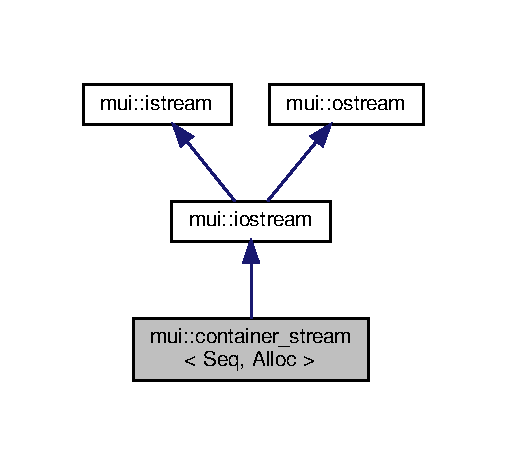
\includegraphics[width=244pt]{classmui_1_1container__stream__inherit__graph}
\end{center}
\end{figure}


Collaboration diagram for mui\+:\+:container\+\_\+stream$<$ Seq, Alloc $>$\+:
\nopagebreak
\begin{figure}[H]
\begin{center}
\leavevmode
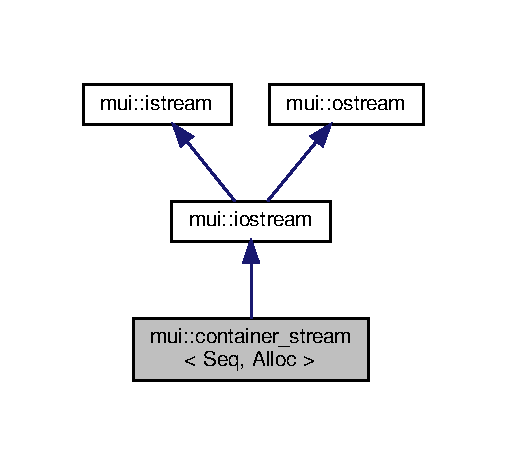
\includegraphics[width=244pt]{classmui_1_1container__stream__coll__graph}
\end{center}
\end{figure}
\subsection*{Public Member Functions}
\begin{DoxyCompactItemize}
\item 
\hyperlink{classmui_1_1container__stream_ac544641054e5769092d239a679aec064}{$\sim$container\+\_\+stream} ()
\item 
void \hyperlink{classmui_1_1container__stream_a6bcd220029a12f27de5443a2b48b245a}{read} (char $\ast$ptr, std\+::size\+\_\+t size)
\item 
void \hyperlink{classmui_1_1container__stream_a47bb31cd5e33311702d15e43f87cdc92}{write} (const char $\ast$ptr, std\+::size\+\_\+t size)
\item 
Seq$<$ char, Alloc $>$ \& \hyperlink{classmui_1_1container__stream_a8c71e91aa411bba0cae4b8837961a621}{data} ()
\item 
const Seq$<$ char, Alloc $>$ \& \hyperlink{classmui_1_1container__stream_a205a767916f764fc96055c87186c1229}{data} () const
\end{DoxyCompactItemize}


\subsection{Constructor \& Destructor Documentation}
\mbox{\Hypertarget{classmui_1_1container__stream_ac544641054e5769092d239a679aec064}\label{classmui_1_1container__stream_ac544641054e5769092d239a679aec064}} 
\index{mui\+::container\+\_\+stream@{mui\+::container\+\_\+stream}!````~container\+\_\+stream@{$\sim$container\+\_\+stream}}
\index{````~container\+\_\+stream@{$\sim$container\+\_\+stream}!mui\+::container\+\_\+stream@{mui\+::container\+\_\+stream}}
\subsubsection{\texorpdfstring{$\sim$container\+\_\+stream()}{~container\_stream()}}
{\footnotesize\ttfamily template$<$template$<$ typename T, typename=std\+::allocator$<$ T $>$ $>$ class Seq, typename Alloc  = std\+::allocator$<$char$>$$>$ \\
\hyperlink{classmui_1_1container__stream}{mui\+::container\+\_\+stream}$<$ Seq, Alloc $>$\+::$\sim$\hyperlink{classmui_1_1container__stream}{container\+\_\+stream} (\begin{DoxyParamCaption}{ }\end{DoxyParamCaption})\hspace{0.3cm}{\ttfamily [inline]}}



\subsection{Member Function Documentation}
\mbox{\Hypertarget{classmui_1_1container__stream_a8c71e91aa411bba0cae4b8837961a621}\label{classmui_1_1container__stream_a8c71e91aa411bba0cae4b8837961a621}} 
\index{mui\+::container\+\_\+stream@{mui\+::container\+\_\+stream}!data@{data}}
\index{data@{data}!mui\+::container\+\_\+stream@{mui\+::container\+\_\+stream}}
\subsubsection{\texorpdfstring{data()}{data()}\hspace{0.1cm}{\footnotesize\ttfamily [1/2]}}
{\footnotesize\ttfamily template$<$template$<$ typename T, typename=std\+::allocator$<$ T $>$ $>$ class Seq, typename Alloc  = std\+::allocator$<$char$>$$>$ \\
Seq$<$char,Alloc$>$\& \hyperlink{classmui_1_1container__stream}{mui\+::container\+\_\+stream}$<$ Seq, Alloc $>$\+::data (\begin{DoxyParamCaption}{ }\end{DoxyParamCaption})\hspace{0.3cm}{\ttfamily [inline]}}

\mbox{\Hypertarget{classmui_1_1container__stream_a205a767916f764fc96055c87186c1229}\label{classmui_1_1container__stream_a205a767916f764fc96055c87186c1229}} 
\index{mui\+::container\+\_\+stream@{mui\+::container\+\_\+stream}!data@{data}}
\index{data@{data}!mui\+::container\+\_\+stream@{mui\+::container\+\_\+stream}}
\subsubsection{\texorpdfstring{data()}{data()}\hspace{0.1cm}{\footnotesize\ttfamily [2/2]}}
{\footnotesize\ttfamily template$<$template$<$ typename T, typename=std\+::allocator$<$ T $>$ $>$ class Seq, typename Alloc  = std\+::allocator$<$char$>$$>$ \\
const Seq$<$char,Alloc$>$\& \hyperlink{classmui_1_1container__stream}{mui\+::container\+\_\+stream}$<$ Seq, Alloc $>$\+::data (\begin{DoxyParamCaption}{ }\end{DoxyParamCaption}) const\hspace{0.3cm}{\ttfamily [inline]}}

\mbox{\Hypertarget{classmui_1_1container__stream_a6bcd220029a12f27de5443a2b48b245a}\label{classmui_1_1container__stream_a6bcd220029a12f27de5443a2b48b245a}} 
\index{mui\+::container\+\_\+stream@{mui\+::container\+\_\+stream}!read@{read}}
\index{read@{read}!mui\+::container\+\_\+stream@{mui\+::container\+\_\+stream}}
\subsubsection{\texorpdfstring{read()}{read()}}
{\footnotesize\ttfamily template$<$template$<$ typename T, typename=std\+::allocator$<$ T $>$ $>$ class Seq, typename Alloc  = std\+::allocator$<$char$>$$>$ \\
void \hyperlink{classmui_1_1container__stream}{mui\+::container\+\_\+stream}$<$ Seq, Alloc $>$\+::read (\begin{DoxyParamCaption}\item[{char $\ast$}]{ptr,  }\item[{std\+::size\+\_\+t}]{size }\end{DoxyParamCaption})\hspace{0.3cm}{\ttfamily [inline]}, {\ttfamily [virtual]}}



Implements \hyperlink{classmui_1_1istream_a275ecbe530bf67df5978be288897ab45}{mui\+::istream}.

\mbox{\Hypertarget{classmui_1_1container__stream_a47bb31cd5e33311702d15e43f87cdc92}\label{classmui_1_1container__stream_a47bb31cd5e33311702d15e43f87cdc92}} 
\index{mui\+::container\+\_\+stream@{mui\+::container\+\_\+stream}!write@{write}}
\index{write@{write}!mui\+::container\+\_\+stream@{mui\+::container\+\_\+stream}}
\subsubsection{\texorpdfstring{write()}{write()}}
{\footnotesize\ttfamily template$<$template$<$ typename T, typename=std\+::allocator$<$ T $>$ $>$ class Seq, typename Alloc  = std\+::allocator$<$char$>$$>$ \\
void \hyperlink{classmui_1_1container__stream}{mui\+::container\+\_\+stream}$<$ Seq, Alloc $>$\+::write (\begin{DoxyParamCaption}\item[{const char $\ast$}]{ptr,  }\item[{std\+::size\+\_\+t}]{size }\end{DoxyParamCaption})\hspace{0.3cm}{\ttfamily [inline]}, {\ttfamily [virtual]}}



Implements \hyperlink{classmui_1_1ostream_a93a0a1d32007efc375d885181c833995}{mui\+::ostream}.



The documentation for this class was generated from the following file\+:\begin{DoxyCompactItemize}
\item 
\hyperlink{stream_8h}{stream.\+h}\end{DoxyCompactItemize}

\hypertarget{classmui4py_1_1common_1_1_cpp_class}{}\section{mui4py.\+common.\+Cpp\+Class Class Reference}
\label{classmui4py_1_1common_1_1_cpp_class}\index{mui4py.\+common.\+Cpp\+Class@{mui4py.\+common.\+Cpp\+Class}}


Inheritance diagram for mui4py.\+common.\+Cpp\+Class\+:
\nopagebreak
\begin{figure}[H]
\begin{center}
\leavevmode
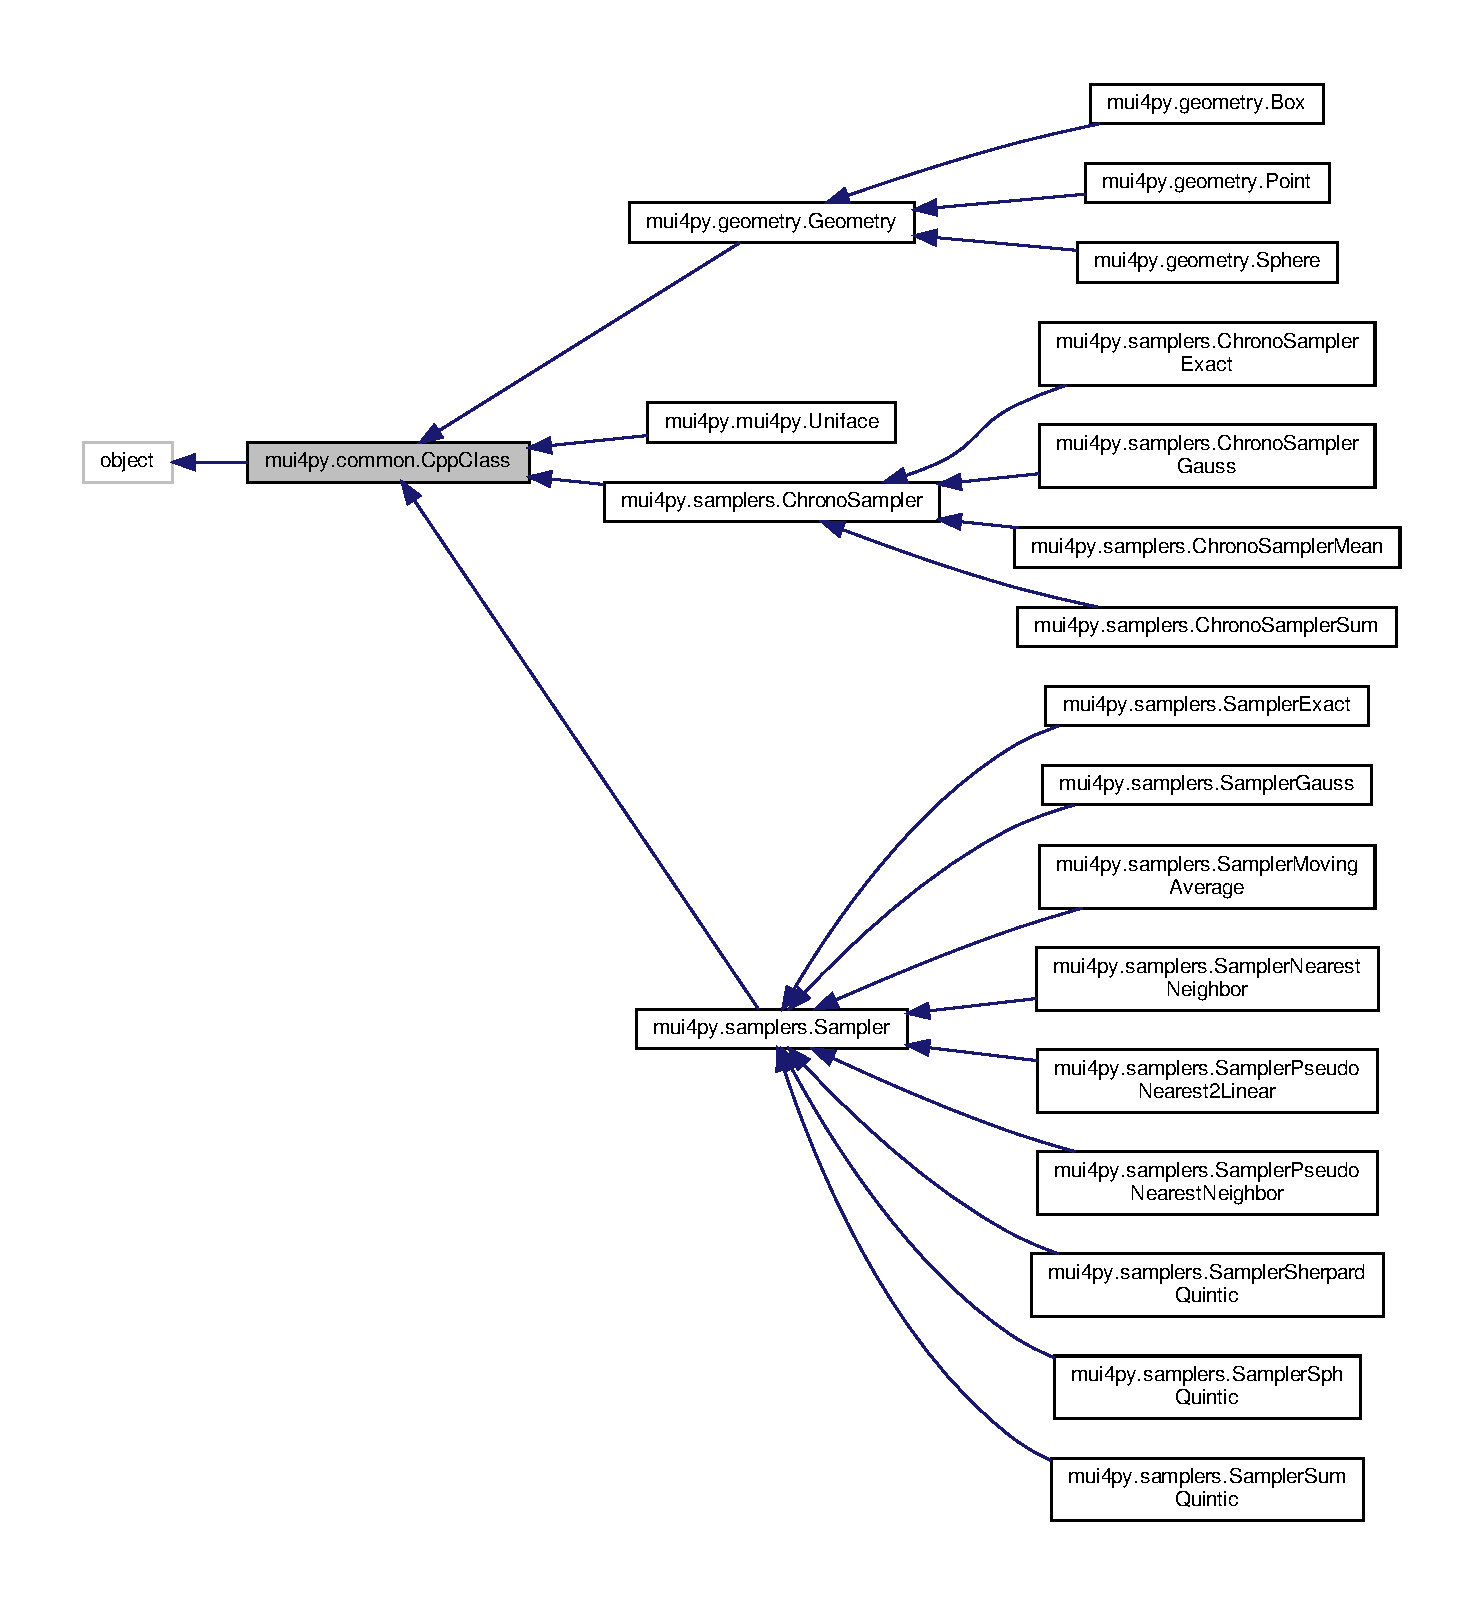
\includegraphics[width=350pt]{classmui4py_1_1common_1_1_cpp_class__inherit__graph}
\end{center}
\end{figure}


Collaboration diagram for mui4py.\+common.\+Cpp\+Class\+:
\nopagebreak
\begin{figure}[H]
\begin{center}
\leavevmode
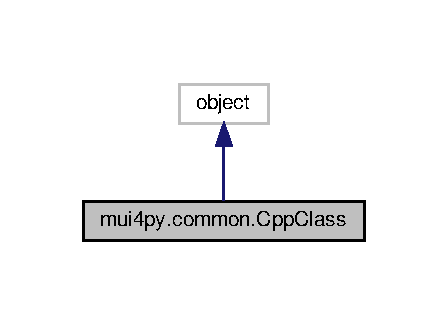
\includegraphics[width=215pt]{classmui4py_1_1common_1_1_cpp_class__coll__graph}
\end{center}
\end{figure}
\subsection*{Public Member Functions}
\begin{DoxyCompactItemize}
\item 
def \hyperlink{classmui4py_1_1common_1_1_cpp_class_af71dd873bcff2f831b48d0d81f900c16}{\+\_\+\+\_\+init\+\_\+\+\_\+} (self, \hyperlink{classmui4py_1_1common_1_1_cpp_class_ac0ad2501063d600bb0101a269a817ce8}{config}=None, \hyperlink{classmui4py_1_1common_1_1_cpp_class_a29797823c6e21f22bba24ee7d35ef31d}{args}=(), \hyperlink{classmui4py_1_1common_1_1_cpp_class_af43879f06f07b1abf0d08e30c5ead46f}{kwargs}=\{\})
\item 
def \hyperlink{classmui4py_1_1common_1_1_cpp_class_a255b3ad646751b5ed10c1795638275e1}{get\+\_\+plain\+\_\+args} (self)
\item 
def \hyperlink{classmui4py_1_1common_1_1_cpp_class_a646e7d435bd4a8b053103bbc8b2368d7}{get\+\_\+plain\+\_\+kwargs} (self)
\item 
def \hyperlink{classmui4py_1_1common_1_1_cpp_class_a72df33d8f73522f22a53f2d476eda586}{configure} (self, \hyperlink{classmui4py_1_1common_1_1_cpp_class_ac0ad2501063d600bb0101a269a817ce8}{config}, \hyperlink{classmui4py_1_1common_1_1_cpp_class_a32aeb99991acd0d8d8604984099dc010}{io\+\_\+data\+\_\+type}=None, cpp\+\_\+obj=None, onlycheck=False)
\end{DoxyCompactItemize}
\subsection*{Public Attributes}
\begin{DoxyCompactItemize}
\item 
\hyperlink{classmui4py_1_1common_1_1_cpp_class_a74f857985586bedbfc71877feab9bb35}{raw\+\_\+point}
\item 
\hyperlink{classmui4py_1_1common_1_1_cpp_class_a7cd72d9f15e0159ec4124eee61861222}{raw}
\item 
\hyperlink{classmui4py_1_1common_1_1_cpp_class_a32aeb99991acd0d8d8604984099dc010}{io\+\_\+data\+\_\+type}
\item 
\hyperlink{classmui4py_1_1common_1_1_cpp_class_a29797823c6e21f22bba24ee7d35ef31d}{args}
\item 
\hyperlink{classmui4py_1_1common_1_1_cpp_class_aa45aca5328de14c2baa089fc9087f3cf}{namespace}
\item 
\hyperlink{classmui4py_1_1common_1_1_cpp_class_af43879f06f07b1abf0d08e30c5ead46f}{kwargs}
\item 
\hyperlink{classmui4py_1_1common_1_1_cpp_class_a7c23ce0b5a2dd5e8a255e5d27c2dd595}{configured}
\item 
\hyperlink{classmui4py_1_1common_1_1_cpp_class_ac0ad2501063d600bb0101a269a817ce8}{config}
\item 
\hyperlink{classmui4py_1_1common_1_1_cpp_class_acab1a6431c2c8d5c1ca73bd643199ff4}{signature}
\item 
\hyperlink{classmui4py_1_1common_1_1_cpp_class_ac7358f958eba2fdbbbdf1d945d2f0a3c}{point\+\_\+class\+\_\+name}
\end{DoxyCompactItemize}


\subsection{Constructor \& Destructor Documentation}
\mbox{\Hypertarget{classmui4py_1_1common_1_1_cpp_class_af71dd873bcff2f831b48d0d81f900c16}\label{classmui4py_1_1common_1_1_cpp_class_af71dd873bcff2f831b48d0d81f900c16}} 
\index{mui4py\+::common\+::\+Cpp\+Class@{mui4py\+::common\+::\+Cpp\+Class}!\+\_\+\+\_\+init\+\_\+\+\_\+@{\+\_\+\+\_\+init\+\_\+\+\_\+}}
\index{\+\_\+\+\_\+init\+\_\+\+\_\+@{\+\_\+\+\_\+init\+\_\+\+\_\+}!mui4py\+::common\+::\+Cpp\+Class@{mui4py\+::common\+::\+Cpp\+Class}}
\subsubsection{\texorpdfstring{\+\_\+\+\_\+init\+\_\+\+\_\+()}{\_\_init\_\_()}}
{\footnotesize\ttfamily def mui4py.\+common.\+Cpp\+Class.\+\_\+\+\_\+init\+\_\+\+\_\+ (\begin{DoxyParamCaption}\item[{}]{self,  }\item[{}]{config = {\ttfamily None},  }\item[{}]{args = {\ttfamily ()},  }\item[{}]{kwargs = {\ttfamily \{\}} }\end{DoxyParamCaption})}



\subsection{Member Function Documentation}
\mbox{\Hypertarget{classmui4py_1_1common_1_1_cpp_class_a72df33d8f73522f22a53f2d476eda586}\label{classmui4py_1_1common_1_1_cpp_class_a72df33d8f73522f22a53f2d476eda586}} 
\index{mui4py\+::common\+::\+Cpp\+Class@{mui4py\+::common\+::\+Cpp\+Class}!configure@{configure}}
\index{configure@{configure}!mui4py\+::common\+::\+Cpp\+Class@{mui4py\+::common\+::\+Cpp\+Class}}
\subsubsection{\texorpdfstring{configure()}{configure()}}
{\footnotesize\ttfamily def mui4py.\+common.\+Cpp\+Class.\+configure (\begin{DoxyParamCaption}\item[{}]{self,  }\item[{}]{config,  }\item[{}]{io\+\_\+data\+\_\+type = {\ttfamily None},  }\item[{}]{cpp\+\_\+obj = {\ttfamily None},  }\item[{}]{onlycheck = {\ttfamily False} }\end{DoxyParamCaption})}

\mbox{\Hypertarget{classmui4py_1_1common_1_1_cpp_class_a255b3ad646751b5ed10c1795638275e1}\label{classmui4py_1_1common_1_1_cpp_class_a255b3ad646751b5ed10c1795638275e1}} 
\index{mui4py\+::common\+::\+Cpp\+Class@{mui4py\+::common\+::\+Cpp\+Class}!get\+\_\+plain\+\_\+args@{get\+\_\+plain\+\_\+args}}
\index{get\+\_\+plain\+\_\+args@{get\+\_\+plain\+\_\+args}!mui4py\+::common\+::\+Cpp\+Class@{mui4py\+::common\+::\+Cpp\+Class}}
\subsubsection{\texorpdfstring{get\+\_\+plain\+\_\+args()}{get\_plain\_args()}}
{\footnotesize\ttfamily def mui4py.\+common.\+Cpp\+Class.\+get\+\_\+plain\+\_\+args (\begin{DoxyParamCaption}\item[{}]{self }\end{DoxyParamCaption})}

\mbox{\Hypertarget{classmui4py_1_1common_1_1_cpp_class_a646e7d435bd4a8b053103bbc8b2368d7}\label{classmui4py_1_1common_1_1_cpp_class_a646e7d435bd4a8b053103bbc8b2368d7}} 
\index{mui4py\+::common\+::\+Cpp\+Class@{mui4py\+::common\+::\+Cpp\+Class}!get\+\_\+plain\+\_\+kwargs@{get\+\_\+plain\+\_\+kwargs}}
\index{get\+\_\+plain\+\_\+kwargs@{get\+\_\+plain\+\_\+kwargs}!mui4py\+::common\+::\+Cpp\+Class@{mui4py\+::common\+::\+Cpp\+Class}}
\subsubsection{\texorpdfstring{get\+\_\+plain\+\_\+kwargs()}{get\_plain\_kwargs()}}
{\footnotesize\ttfamily def mui4py.\+common.\+Cpp\+Class.\+get\+\_\+plain\+\_\+kwargs (\begin{DoxyParamCaption}\item[{}]{self }\end{DoxyParamCaption})}



\subsection{Member Data Documentation}
\mbox{\Hypertarget{classmui4py_1_1common_1_1_cpp_class_a29797823c6e21f22bba24ee7d35ef31d}\label{classmui4py_1_1common_1_1_cpp_class_a29797823c6e21f22bba24ee7d35ef31d}} 
\index{mui4py\+::common\+::\+Cpp\+Class@{mui4py\+::common\+::\+Cpp\+Class}!args@{args}}
\index{args@{args}!mui4py\+::common\+::\+Cpp\+Class@{mui4py\+::common\+::\+Cpp\+Class}}
\subsubsection{\texorpdfstring{args}{args}}
{\footnotesize\ttfamily mui4py.\+common.\+Cpp\+Class.\+args}

\mbox{\Hypertarget{classmui4py_1_1common_1_1_cpp_class_ac0ad2501063d600bb0101a269a817ce8}\label{classmui4py_1_1common_1_1_cpp_class_ac0ad2501063d600bb0101a269a817ce8}} 
\index{mui4py\+::common\+::\+Cpp\+Class@{mui4py\+::common\+::\+Cpp\+Class}!config@{config}}
\index{config@{config}!mui4py\+::common\+::\+Cpp\+Class@{mui4py\+::common\+::\+Cpp\+Class}}
\subsubsection{\texorpdfstring{config}{config}}
{\footnotesize\ttfamily mui4py.\+common.\+Cpp\+Class.\+config}

\mbox{\Hypertarget{classmui4py_1_1common_1_1_cpp_class_a7c23ce0b5a2dd5e8a255e5d27c2dd595}\label{classmui4py_1_1common_1_1_cpp_class_a7c23ce0b5a2dd5e8a255e5d27c2dd595}} 
\index{mui4py\+::common\+::\+Cpp\+Class@{mui4py\+::common\+::\+Cpp\+Class}!configured@{configured}}
\index{configured@{configured}!mui4py\+::common\+::\+Cpp\+Class@{mui4py\+::common\+::\+Cpp\+Class}}
\subsubsection{\texorpdfstring{configured}{configured}}
{\footnotesize\ttfamily mui4py.\+common.\+Cpp\+Class.\+configured}

\mbox{\Hypertarget{classmui4py_1_1common_1_1_cpp_class_a32aeb99991acd0d8d8604984099dc010}\label{classmui4py_1_1common_1_1_cpp_class_a32aeb99991acd0d8d8604984099dc010}} 
\index{mui4py\+::common\+::\+Cpp\+Class@{mui4py\+::common\+::\+Cpp\+Class}!io\+\_\+data\+\_\+type@{io\+\_\+data\+\_\+type}}
\index{io\+\_\+data\+\_\+type@{io\+\_\+data\+\_\+type}!mui4py\+::common\+::\+Cpp\+Class@{mui4py\+::common\+::\+Cpp\+Class}}
\subsubsection{\texorpdfstring{io\+\_\+data\+\_\+type}{io\_data\_type}}
{\footnotesize\ttfamily mui4py.\+common.\+Cpp\+Class.\+io\+\_\+data\+\_\+type}

\mbox{\Hypertarget{classmui4py_1_1common_1_1_cpp_class_af43879f06f07b1abf0d08e30c5ead46f}\label{classmui4py_1_1common_1_1_cpp_class_af43879f06f07b1abf0d08e30c5ead46f}} 
\index{mui4py\+::common\+::\+Cpp\+Class@{mui4py\+::common\+::\+Cpp\+Class}!kwargs@{kwargs}}
\index{kwargs@{kwargs}!mui4py\+::common\+::\+Cpp\+Class@{mui4py\+::common\+::\+Cpp\+Class}}
\subsubsection{\texorpdfstring{kwargs}{kwargs}}
{\footnotesize\ttfamily mui4py.\+common.\+Cpp\+Class.\+kwargs}

\mbox{\Hypertarget{classmui4py_1_1common_1_1_cpp_class_aa45aca5328de14c2baa089fc9087f3cf}\label{classmui4py_1_1common_1_1_cpp_class_aa45aca5328de14c2baa089fc9087f3cf}} 
\index{mui4py\+::common\+::\+Cpp\+Class@{mui4py\+::common\+::\+Cpp\+Class}!namespace@{namespace}}
\index{namespace@{namespace}!mui4py\+::common\+::\+Cpp\+Class@{mui4py\+::common\+::\+Cpp\+Class}}
\subsubsection{\texorpdfstring{namespace}{namespace}}
{\footnotesize\ttfamily mui4py.\+common.\+Cpp\+Class.\+namespace}

\mbox{\Hypertarget{classmui4py_1_1common_1_1_cpp_class_ac7358f958eba2fdbbbdf1d945d2f0a3c}\label{classmui4py_1_1common_1_1_cpp_class_ac7358f958eba2fdbbbdf1d945d2f0a3c}} 
\index{mui4py\+::common\+::\+Cpp\+Class@{mui4py\+::common\+::\+Cpp\+Class}!point\+\_\+class\+\_\+name@{point\+\_\+class\+\_\+name}}
\index{point\+\_\+class\+\_\+name@{point\+\_\+class\+\_\+name}!mui4py\+::common\+::\+Cpp\+Class@{mui4py\+::common\+::\+Cpp\+Class}}
\subsubsection{\texorpdfstring{point\+\_\+class\+\_\+name}{point\_class\_name}}
{\footnotesize\ttfamily mui4py.\+common.\+Cpp\+Class.\+point\+\_\+class\+\_\+name}

\mbox{\Hypertarget{classmui4py_1_1common_1_1_cpp_class_a7cd72d9f15e0159ec4124eee61861222}\label{classmui4py_1_1common_1_1_cpp_class_a7cd72d9f15e0159ec4124eee61861222}} 
\index{mui4py\+::common\+::\+Cpp\+Class@{mui4py\+::common\+::\+Cpp\+Class}!raw@{raw}}
\index{raw@{raw}!mui4py\+::common\+::\+Cpp\+Class@{mui4py\+::common\+::\+Cpp\+Class}}
\subsubsection{\texorpdfstring{raw}{raw}}
{\footnotesize\ttfamily mui4py.\+common.\+Cpp\+Class.\+raw}

\mbox{\Hypertarget{classmui4py_1_1common_1_1_cpp_class_a74f857985586bedbfc71877feab9bb35}\label{classmui4py_1_1common_1_1_cpp_class_a74f857985586bedbfc71877feab9bb35}} 
\index{mui4py\+::common\+::\+Cpp\+Class@{mui4py\+::common\+::\+Cpp\+Class}!raw\+\_\+point@{raw\+\_\+point}}
\index{raw\+\_\+point@{raw\+\_\+point}!mui4py\+::common\+::\+Cpp\+Class@{mui4py\+::common\+::\+Cpp\+Class}}
\subsubsection{\texorpdfstring{raw\+\_\+point}{raw\_point}}
{\footnotesize\ttfamily mui4py.\+common.\+Cpp\+Class.\+raw\+\_\+point}

\mbox{\Hypertarget{classmui4py_1_1common_1_1_cpp_class_acab1a6431c2c8d5c1ca73bd643199ff4}\label{classmui4py_1_1common_1_1_cpp_class_acab1a6431c2c8d5c1ca73bd643199ff4}} 
\index{mui4py\+::common\+::\+Cpp\+Class@{mui4py\+::common\+::\+Cpp\+Class}!signature@{signature}}
\index{signature@{signature}!mui4py\+::common\+::\+Cpp\+Class@{mui4py\+::common\+::\+Cpp\+Class}}
\subsubsection{\texorpdfstring{signature}{signature}}
{\footnotesize\ttfamily mui4py.\+common.\+Cpp\+Class.\+signature}



The documentation for this class was generated from the following file\+:\begin{DoxyCompactItemize}
\item 
wrappers/\+Python/mui4py/\hyperlink{common_8py}{common.\+py}\end{DoxyCompactItemize}

\hypertarget{structmui_1_1crunch}{}\section{mui\+:\+:crunch Struct Reference}
\label{structmui_1_1crunch}\index{mui\+::crunch@{mui\+::crunch}}


{\ttfamily \#include $<$config.\+h$>$}



Inheritance diagram for mui\+:\+:crunch\+:
\nopagebreak
\begin{figure}[H]
\begin{center}
\leavevmode
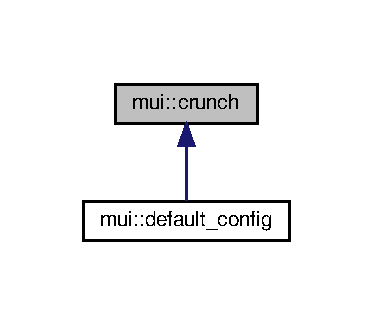
\includegraphics[width=179pt]{structmui_1_1crunch__inherit__graph}
\end{center}
\end{figure}
\subsection*{Public Types}
\begin{DoxyCompactItemize}
\item 
using \hyperlink{structmui_1_1crunch_a6f2cbcc30446f242a8e0a99400d29b69}{R\+E\+AL} = double
\item 
using \hyperlink{structmui_1_1crunch_a85f2c6d604af24d375168cd481228b70}{I\+NT} = int
\item 
using \hyperlink{structmui_1_1crunch_ae91784f5fa63d0dea1dcb4f37fe59ff5}{point\+\_\+type} = \hyperlink{structmui_1_1point}{point}$<$ \hyperlink{structmui_1_1crunch_a6f2cbcc30446f242a8e0a99400d29b69}{R\+E\+AL}, \hyperlink{structmui_1_1crunch_afa49250ca88779f6d39c0ab585120c2b}{D} $>$
\item 
using \hyperlink{structmui_1_1crunch_a6967823168cabd179daab1d81f817eba}{time\+\_\+type} = \hyperlink{structmui_1_1crunch_a6f2cbcc30446f242a8e0a99400d29b69}{R\+E\+AL}
\item 
using \hyperlink{structmui_1_1crunch_a0a0e3d165ddd799123f067a61e66c000}{data\+\_\+types} = \hyperlink{structmui_1_1type__list}{type\+\_\+list}$<$ int, double, float $>$
\item 
using \hyperlink{structmui_1_1crunch_aec04e38b4a056876eb72c8f570621bd5}{E\+X\+C\+E\+P\+T\+I\+ON} = \hyperlink{structmui_1_1exception__segv}{exception\+\_\+segv}
\end{DoxyCompactItemize}
\subsection*{Static Public Attributes}
\begin{DoxyCompactItemize}
\item 
static const int \hyperlink{structmui_1_1crunch_afa49250ca88779f6d39c0ab585120c2b}{D} = 3
\item 
static const bool \hyperlink{structmui_1_1crunch_acb71ed26e49e2d2f1233b1a08b4992c4}{D\+E\+B\+UG} = false
\item 
static const bool \hyperlink{structmui_1_1crunch_a6a715d5981394944a2ce0a12a7048891}{F\+I\+X\+E\+D\+P\+O\+I\+N\+TS} = false
\end{DoxyCompactItemize}


\subsection{Member Typedef Documentation}
\mbox{\Hypertarget{structmui_1_1crunch_a0a0e3d165ddd799123f067a61e66c000}\label{structmui_1_1crunch_a0a0e3d165ddd799123f067a61e66c000}} 
\index{mui\+::crunch@{mui\+::crunch}!data\+\_\+types@{data\+\_\+types}}
\index{data\+\_\+types@{data\+\_\+types}!mui\+::crunch@{mui\+::crunch}}
\subsubsection{\texorpdfstring{data\+\_\+types}{data\_types}}
{\footnotesize\ttfamily using \hyperlink{structmui_1_1crunch_a0a0e3d165ddd799123f067a61e66c000}{mui\+::crunch\+::data\+\_\+types} =  \hyperlink{structmui_1_1type__list}{type\+\_\+list}$<$int,double,float$>$}

\mbox{\Hypertarget{structmui_1_1crunch_aec04e38b4a056876eb72c8f570621bd5}\label{structmui_1_1crunch_aec04e38b4a056876eb72c8f570621bd5}} 
\index{mui\+::crunch@{mui\+::crunch}!E\+X\+C\+E\+P\+T\+I\+ON@{E\+X\+C\+E\+P\+T\+I\+ON}}
\index{E\+X\+C\+E\+P\+T\+I\+ON@{E\+X\+C\+E\+P\+T\+I\+ON}!mui\+::crunch@{mui\+::crunch}}
\subsubsection{\texorpdfstring{E\+X\+C\+E\+P\+T\+I\+ON}{EXCEPTION}}
{\footnotesize\ttfamily using \hyperlink{structmui_1_1crunch_aec04e38b4a056876eb72c8f570621bd5}{mui\+::crunch\+::\+E\+X\+C\+E\+P\+T\+I\+ON} =  \hyperlink{structmui_1_1exception__segv}{exception\+\_\+segv}}

\mbox{\Hypertarget{structmui_1_1crunch_a85f2c6d604af24d375168cd481228b70}\label{structmui_1_1crunch_a85f2c6d604af24d375168cd481228b70}} 
\index{mui\+::crunch@{mui\+::crunch}!I\+NT@{I\+NT}}
\index{I\+NT@{I\+NT}!mui\+::crunch@{mui\+::crunch}}
\subsubsection{\texorpdfstring{I\+NT}{INT}}
{\footnotesize\ttfamily using \hyperlink{structmui_1_1crunch_a85f2c6d604af24d375168cd481228b70}{mui\+::crunch\+::\+I\+NT} =  int}

\mbox{\Hypertarget{structmui_1_1crunch_ae91784f5fa63d0dea1dcb4f37fe59ff5}\label{structmui_1_1crunch_ae91784f5fa63d0dea1dcb4f37fe59ff5}} 
\index{mui\+::crunch@{mui\+::crunch}!point\+\_\+type@{point\+\_\+type}}
\index{point\+\_\+type@{point\+\_\+type}!mui\+::crunch@{mui\+::crunch}}
\subsubsection{\texorpdfstring{point\+\_\+type}{point\_type}}
{\footnotesize\ttfamily using \hyperlink{structmui_1_1crunch_ae91784f5fa63d0dea1dcb4f37fe59ff5}{mui\+::crunch\+::point\+\_\+type} =  \hyperlink{structmui_1_1point}{point}$<$\hyperlink{structmui_1_1crunch_a6f2cbcc30446f242a8e0a99400d29b69}{R\+E\+AL},\hyperlink{structmui_1_1crunch_afa49250ca88779f6d39c0ab585120c2b}{D}$>$}

\mbox{\Hypertarget{structmui_1_1crunch_a6f2cbcc30446f242a8e0a99400d29b69}\label{structmui_1_1crunch_a6f2cbcc30446f242a8e0a99400d29b69}} 
\index{mui\+::crunch@{mui\+::crunch}!R\+E\+AL@{R\+E\+AL}}
\index{R\+E\+AL@{R\+E\+AL}!mui\+::crunch@{mui\+::crunch}}
\subsubsection{\texorpdfstring{R\+E\+AL}{REAL}}
{\footnotesize\ttfamily using \hyperlink{structmui_1_1crunch_a6f2cbcc30446f242a8e0a99400d29b69}{mui\+::crunch\+::\+R\+E\+AL} =  double}

\mbox{\Hypertarget{structmui_1_1crunch_a6967823168cabd179daab1d81f817eba}\label{structmui_1_1crunch_a6967823168cabd179daab1d81f817eba}} 
\index{mui\+::crunch@{mui\+::crunch}!time\+\_\+type@{time\+\_\+type}}
\index{time\+\_\+type@{time\+\_\+type}!mui\+::crunch@{mui\+::crunch}}
\subsubsection{\texorpdfstring{time\+\_\+type}{time\_type}}
{\footnotesize\ttfamily using \hyperlink{structmui_1_1crunch_a6967823168cabd179daab1d81f817eba}{mui\+::crunch\+::time\+\_\+type} =  \hyperlink{structmui_1_1crunch_a6f2cbcc30446f242a8e0a99400d29b69}{R\+E\+AL}}



\subsection{Member Data Documentation}
\mbox{\Hypertarget{structmui_1_1crunch_afa49250ca88779f6d39c0ab585120c2b}\label{structmui_1_1crunch_afa49250ca88779f6d39c0ab585120c2b}} 
\index{mui\+::crunch@{mui\+::crunch}!D@{D}}
\index{D@{D}!mui\+::crunch@{mui\+::crunch}}
\subsubsection{\texorpdfstring{D}{D}}
{\footnotesize\ttfamily const int mui\+::crunch\+::D = 3\hspace{0.3cm}{\ttfamily [static]}}

\mbox{\Hypertarget{structmui_1_1crunch_acb71ed26e49e2d2f1233b1a08b4992c4}\label{structmui_1_1crunch_acb71ed26e49e2d2f1233b1a08b4992c4}} 
\index{mui\+::crunch@{mui\+::crunch}!D\+E\+B\+UG@{D\+E\+B\+UG}}
\index{D\+E\+B\+UG@{D\+E\+B\+UG}!mui\+::crunch@{mui\+::crunch}}
\subsubsection{\texorpdfstring{D\+E\+B\+UG}{DEBUG}}
{\footnotesize\ttfamily const bool mui\+::crunch\+::\+D\+E\+B\+UG = false\hspace{0.3cm}{\ttfamily [static]}}

\mbox{\Hypertarget{structmui_1_1crunch_a6a715d5981394944a2ce0a12a7048891}\label{structmui_1_1crunch_a6a715d5981394944a2ce0a12a7048891}} 
\index{mui\+::crunch@{mui\+::crunch}!F\+I\+X\+E\+D\+P\+O\+I\+N\+TS@{F\+I\+X\+E\+D\+P\+O\+I\+N\+TS}}
\index{F\+I\+X\+E\+D\+P\+O\+I\+N\+TS@{F\+I\+X\+E\+D\+P\+O\+I\+N\+TS}!mui\+::crunch@{mui\+::crunch}}
\subsubsection{\texorpdfstring{F\+I\+X\+E\+D\+P\+O\+I\+N\+TS}{FIXEDPOINTS}}
{\footnotesize\ttfamily const bool mui\+::crunch\+::\+F\+I\+X\+E\+D\+P\+O\+I\+N\+TS = false\hspace{0.3cm}{\ttfamily [static]}}



The documentation for this struct was generated from the following file\+:\begin{DoxyCompactItemize}
\item 
\hyperlink{config_8h}{config.\+h}\end{DoxyCompactItemize}

\hypertarget{unionmui_1_1detail_1_1endian__converter_1_1data__t}{}\section{mui\+:\+:detail\+:\+:endian\+\_\+converter$<$ size\+\_\+bytes $>$\+:\+:data\+\_\+t Union Reference}
\label{unionmui_1_1detail_1_1endian__converter_1_1data__t}\index{mui\+::detail\+::endian\+\_\+converter$<$ size\+\_\+bytes $>$\+::data\+\_\+t@{mui\+::detail\+::endian\+\_\+converter$<$ size\+\_\+bytes $>$\+::data\+\_\+t}}


{\ttfamily \#include $<$endian\+\_\+traits.\+h$>$}

\subsection*{Public Attributes}
\begin{DoxyCompactItemize}
\item 
char \hyperlink{unionmui_1_1detail_1_1endian__converter_1_1data__t_a2d3bae8b5e2deebe720672203e92326f}{buf} \mbox{[}size\+\_\+bytes\mbox{]}
\item 
\hyperlink{structmui_1_1detail_1_1uint}{uint}$<$ size\+\_\+bytes $>$\+::type \hyperlink{unionmui_1_1detail_1_1endian__converter_1_1data__t_a417cac59882efbad398883100aa83b42}{val}
\end{DoxyCompactItemize}


\subsection{Member Data Documentation}
\mbox{\Hypertarget{unionmui_1_1detail_1_1endian__converter_1_1data__t_a2d3bae8b5e2deebe720672203e92326f}\label{unionmui_1_1detail_1_1endian__converter_1_1data__t_a2d3bae8b5e2deebe720672203e92326f}} 
\index{mui\+::detail\+::endian\+\_\+converter\+::data\+\_\+t@{mui\+::detail\+::endian\+\_\+converter\+::data\+\_\+t}!buf@{buf}}
\index{buf@{buf}!mui\+::detail\+::endian\+\_\+converter\+::data\+\_\+t@{mui\+::detail\+::endian\+\_\+converter\+::data\+\_\+t}}
\subsubsection{\texorpdfstring{buf}{buf}}
{\footnotesize\ttfamily template$<$size\+\_\+t size\+\_\+bytes$>$ \\
char \hyperlink{structmui_1_1detail_1_1endian__converter}{mui\+::detail\+::endian\+\_\+converter}$<$ size\+\_\+bytes $>$\+::data\+\_\+t\+::buf\mbox{[}size\+\_\+bytes\mbox{]}}

\mbox{\Hypertarget{unionmui_1_1detail_1_1endian__converter_1_1data__t_a417cac59882efbad398883100aa83b42}\label{unionmui_1_1detail_1_1endian__converter_1_1data__t_a417cac59882efbad398883100aa83b42}} 
\index{mui\+::detail\+::endian\+\_\+converter\+::data\+\_\+t@{mui\+::detail\+::endian\+\_\+converter\+::data\+\_\+t}!val@{val}}
\index{val@{val}!mui\+::detail\+::endian\+\_\+converter\+::data\+\_\+t@{mui\+::detail\+::endian\+\_\+converter\+::data\+\_\+t}}
\subsubsection{\texorpdfstring{val}{val}}
{\footnotesize\ttfamily template$<$size\+\_\+t size\+\_\+bytes$>$ \\
\hyperlink{structmui_1_1detail_1_1uint}{uint}$<$size\+\_\+bytes$>$\+::type \hyperlink{structmui_1_1detail_1_1endian__converter}{mui\+::detail\+::endian\+\_\+converter}$<$ size\+\_\+bytes $>$\+::data\+\_\+t\+::val}



The documentation for this union was generated from the following file\+:\begin{DoxyCompactItemize}
\item 
\hyperlink{endian__traits_8h}{endian\+\_\+traits.\+h}\end{DoxyCompactItemize}

\hypertarget{structmui_1_1default__config}{}\section{mui\+:\+:default\+\_\+config Struct Reference}
\label{structmui_1_1default__config}\index{mui\+::default\+\_\+config@{mui\+::default\+\_\+config}}


{\ttfamily \#include $<$config.\+h$>$}



Inheritance diagram for mui\+:\+:default\+\_\+config\+:
\nopagebreak
\begin{figure}[H]
\begin{center}
\leavevmode
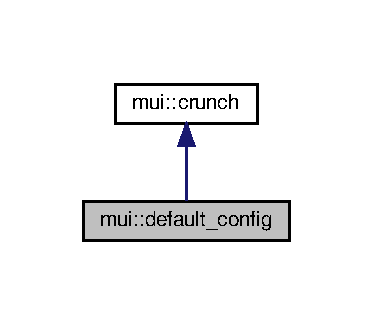
\includegraphics[width=179pt]{structmui_1_1default__config__inherit__graph}
\end{center}
\end{figure}


Collaboration diagram for mui\+:\+:default\+\_\+config\+:
\nopagebreak
\begin{figure}[H]
\begin{center}
\leavevmode
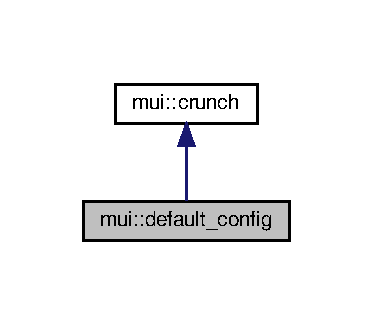
\includegraphics[width=179pt]{structmui_1_1default__config__coll__graph}
\end{center}
\end{figure}
\subsection*{Additional Inherited Members}


The documentation for this struct was generated from the following file\+:\begin{DoxyCompactItemize}
\item 
\hyperlink{config_8h}{config.\+h}\end{DoxyCompactItemize}

\hypertarget{structmui_1_1dim_1_1dim}{}\section{mui\+:\+:dim\+:\+:dim$<$ M\+L\+T\+T\+A\+E\+LI $>$ Struct Template Reference}
\label{structmui_1_1dim_1_1dim}\index{mui\+::dim\+::dim$<$ M\+L\+T\+T\+A\+E\+L\+I $>$@{mui\+::dim\+::dim$<$ M\+L\+T\+T\+A\+E\+L\+I $>$}}


{\ttfamily \#include $<$dim.\+h$>$}

\subsection*{Public Member Functions}
\begin{DoxyCompactItemize}
\item 
\hyperlink{structmui_1_1dim_1_1dim_ad5222f9fcfd07db9c132003b4544ff76}{dim} ()
\item 
\hyperlink{structmui_1_1dim_1_1dim_a8a9104f25986d886cdd98a3e8abdd65d}{dim} (double \+\_\+a\+\_\+)
\item 
\hyperlink{structmui_1_1dim_1_1dim_a740a39809e358db97b0c1a00317e678f}{dim} (const \hyperlink{structmui_1_1dim_1_1dim}{dim} \&other)
\item 
{\footnotesize template$<$int... A\+N\+O\+T\+H\+E\+R\+\_\+\+M\+L\+T\+T\+A\+E\+LI$>$ }\\\hyperlink{structmui_1_1dim_1_1dim_aef3b03be0f2d4385d189eb02675a2a16}{dim} (const \hyperlink{structmui_1_1dim_1_1dim}{dim}$<$ A\+N\+O\+T\+H\+E\+R\+\_\+\+M\+L\+T\+T\+A\+E\+L\+I... $>$ \&error)
\item 
\hyperlink{structmui_1_1dim_1_1dim}{dim} \& \hyperlink{structmui_1_1dim_1_1dim_a59aeac99c9356fd0c44d21ed6bbf9ae7}{operator=} (const \hyperlink{structmui_1_1dim_1_1dim}{dim} \&other)
\item 
{\footnotesize template$<$int... A\+N\+O\+T\+H\+E\+R\+\_\+\+M\+L\+T\+T\+A\+E\+LI$>$ }\\class Cannot\+\_\+\+Assign\+\_\+\+Quantities\+\_\+\+With\+\_\+\+Incompatible\+\_\+\+Dimensionalities \hyperlink{structmui_1_1dim_1_1dim_a05ee5bceb54e51d08bf9f3e99461160e}{operator=} (const \hyperlink{structmui_1_1dim_1_1dim}{dim}$<$ A\+N\+O\+T\+H\+E\+R\+\_\+\+M\+L\+T\+T\+A\+E\+L\+I... $>$ \&other)
\item 
\hyperlink{structmui_1_1dim_1_1dim_a918d850a1a6585ee8a4147b10f5c4998}{operator double} ()
\item 
\hyperlink{structmui_1_1dim_1_1dim}{dim} \hyperlink{structmui_1_1dim_1_1dim_ad3a650609305c544581a749cb338a50b}{convert\+\_\+to} (const \hyperlink{structmui_1_1dim_1_1dim}{dim} \&other)
\item 
{\footnotesize template$<$int... A\+N\+O\+T\+H\+E\+R\+\_\+\+M\+L\+T\+T\+A\+E\+LI$>$ }\\class Cannot\+\_\+\+Assign\+\_\+\+Quantities\+\_\+\+With\+\_\+\+Incompatible\+\_\+\+Dimensionalities \hyperlink{structmui_1_1dim_1_1dim_a3004be3cf40d7fed041b18eb841687ac}{convert\+\_\+to} (const \hyperlink{structmui_1_1dim_1_1dim}{dim}$<$ A\+N\+O\+T\+H\+E\+R\+\_\+\+M\+L\+T\+T\+A\+E\+L\+I... $>$ \&other)
\end{DoxyCompactItemize}
\subsection*{Public Attributes}
\begin{DoxyCompactItemize}
\item 
double \hyperlink{structmui_1_1dim_1_1dim_a40ca9d786e371cc4dd9c125fa99980e6}{a}
\end{DoxyCompactItemize}
\subsection*{Friends}
\begin{DoxyCompactItemize}
\item 
\hyperlink{classmui_1_1ostream}{ostream} \& \hyperlink{structmui_1_1dim_1_1dim_a3e283b43c057fa9d4ffa33f88c7bb7fd}{operator$<$$<$} (\hyperlink{classmui_1_1ostream}{ostream} \&out, \hyperlink{structmui_1_1dim_1_1dim}{dim} q)
\item 
\hyperlink{classmui_1_1istream}{istream} \& \hyperlink{structmui_1_1dim_1_1dim_a933072e8c2019385aba3cbfcd6469186}{operator$>$$>$} (\hyperlink{classmui_1_1istream}{istream} \&in, \hyperlink{structmui_1_1dim_1_1dim}{dim} q)
\end{DoxyCompactItemize}


\subsection{Constructor \& Destructor Documentation}
\mbox{\Hypertarget{structmui_1_1dim_1_1dim_ad5222f9fcfd07db9c132003b4544ff76}\label{structmui_1_1dim_1_1dim_ad5222f9fcfd07db9c132003b4544ff76}} 
\index{mui\+::dim\+::dim@{mui\+::dim\+::dim}!dim@{dim}}
\index{dim@{dim}!mui\+::dim\+::dim@{mui\+::dim\+::dim}}
\subsubsection{\texorpdfstring{dim()}{dim()}\hspace{0.1cm}{\footnotesize\ttfamily [1/4]}}
{\footnotesize\ttfamily template$<$int... M\+L\+T\+T\+A\+E\+LI$>$ \\
\hyperlink{structmui_1_1dim_1_1dim}{mui\+::dim\+::dim}$<$ M\+L\+T\+T\+A\+E\+LI $>$\+::\hyperlink{structmui_1_1dim_1_1dim}{dim} (\begin{DoxyParamCaption}{ }\end{DoxyParamCaption})\hspace{0.3cm}{\ttfamily [inline]}}

\mbox{\Hypertarget{structmui_1_1dim_1_1dim_a8a9104f25986d886cdd98a3e8abdd65d}\label{structmui_1_1dim_1_1dim_a8a9104f25986d886cdd98a3e8abdd65d}} 
\index{mui\+::dim\+::dim@{mui\+::dim\+::dim}!dim@{dim}}
\index{dim@{dim}!mui\+::dim\+::dim@{mui\+::dim\+::dim}}
\subsubsection{\texorpdfstring{dim()}{dim()}\hspace{0.1cm}{\footnotesize\ttfamily [2/4]}}
{\footnotesize\ttfamily template$<$int... M\+L\+T\+T\+A\+E\+LI$>$ \\
\hyperlink{structmui_1_1dim_1_1dim}{mui\+::dim\+::dim}$<$ M\+L\+T\+T\+A\+E\+LI $>$\+::\hyperlink{structmui_1_1dim_1_1dim}{dim} (\begin{DoxyParamCaption}\item[{double}]{\+\_\+a\+\_\+ }\end{DoxyParamCaption})\hspace{0.3cm}{\ttfamily [inline]}}

\mbox{\Hypertarget{structmui_1_1dim_1_1dim_a740a39809e358db97b0c1a00317e678f}\label{structmui_1_1dim_1_1dim_a740a39809e358db97b0c1a00317e678f}} 
\index{mui\+::dim\+::dim@{mui\+::dim\+::dim}!dim@{dim}}
\index{dim@{dim}!mui\+::dim\+::dim@{mui\+::dim\+::dim}}
\subsubsection{\texorpdfstring{dim()}{dim()}\hspace{0.1cm}{\footnotesize\ttfamily [3/4]}}
{\footnotesize\ttfamily template$<$int... M\+L\+T\+T\+A\+E\+LI$>$ \\
\hyperlink{structmui_1_1dim_1_1dim}{mui\+::dim\+::dim}$<$ M\+L\+T\+T\+A\+E\+LI $>$\+::\hyperlink{structmui_1_1dim_1_1dim}{dim} (\begin{DoxyParamCaption}\item[{const \hyperlink{structmui_1_1dim_1_1dim}{dim}$<$ M\+L\+T\+T\+A\+E\+LI $>$ \&}]{other }\end{DoxyParamCaption})\hspace{0.3cm}{\ttfamily [inline]}}

\mbox{\Hypertarget{structmui_1_1dim_1_1dim_aef3b03be0f2d4385d189eb02675a2a16}\label{structmui_1_1dim_1_1dim_aef3b03be0f2d4385d189eb02675a2a16}} 
\index{mui\+::dim\+::dim@{mui\+::dim\+::dim}!dim@{dim}}
\index{dim@{dim}!mui\+::dim\+::dim@{mui\+::dim\+::dim}}
\subsubsection{\texorpdfstring{dim()}{dim()}\hspace{0.1cm}{\footnotesize\ttfamily [4/4]}}
{\footnotesize\ttfamily template$<$int... M\+L\+T\+T\+A\+E\+LI$>$ \\
template$<$int... A\+N\+O\+T\+H\+E\+R\+\_\+\+M\+L\+T\+T\+A\+E\+LI$>$ \\
\hyperlink{structmui_1_1dim_1_1dim}{mui\+::dim\+::dim}$<$ M\+L\+T\+T\+A\+E\+LI $>$\+::\hyperlink{structmui_1_1dim_1_1dim}{dim} (\begin{DoxyParamCaption}\item[{const \hyperlink{structmui_1_1dim_1_1dim}{dim}$<$ A\+N\+O\+T\+H\+E\+R\+\_\+\+M\+L\+T\+T\+A\+E\+L\+I... $>$ \&}]{error }\end{DoxyParamCaption})\hspace{0.3cm}{\ttfamily [inline]}}



\subsection{Member Function Documentation}
\mbox{\Hypertarget{structmui_1_1dim_1_1dim_ad3a650609305c544581a749cb338a50b}\label{structmui_1_1dim_1_1dim_ad3a650609305c544581a749cb338a50b}} 
\index{mui\+::dim\+::dim@{mui\+::dim\+::dim}!convert\+\_\+to@{convert\+\_\+to}}
\index{convert\+\_\+to@{convert\+\_\+to}!mui\+::dim\+::dim@{mui\+::dim\+::dim}}
\subsubsection{\texorpdfstring{convert\+\_\+to()}{convert\_to()}\hspace{0.1cm}{\footnotesize\ttfamily [1/2]}}
{\footnotesize\ttfamily template$<$int... M\+L\+T\+T\+A\+E\+LI$>$ \\
\hyperlink{structmui_1_1dim_1_1dim}{dim} \hyperlink{structmui_1_1dim_1_1dim}{mui\+::dim\+::dim}$<$ M\+L\+T\+T\+A\+E\+LI $>$\+::convert\+\_\+to (\begin{DoxyParamCaption}\item[{const \hyperlink{structmui_1_1dim_1_1dim}{dim}$<$ M\+L\+T\+T\+A\+E\+LI $>$ \&}]{other }\end{DoxyParamCaption})\hspace{0.3cm}{\ttfamily [inline]}}

\mbox{\Hypertarget{structmui_1_1dim_1_1dim_a3004be3cf40d7fed041b18eb841687ac}\label{structmui_1_1dim_1_1dim_a3004be3cf40d7fed041b18eb841687ac}} 
\index{mui\+::dim\+::dim@{mui\+::dim\+::dim}!convert\+\_\+to@{convert\+\_\+to}}
\index{convert\+\_\+to@{convert\+\_\+to}!mui\+::dim\+::dim@{mui\+::dim\+::dim}}
\subsubsection{\texorpdfstring{convert\+\_\+to()}{convert\_to()}\hspace{0.1cm}{\footnotesize\ttfamily [2/2]}}
{\footnotesize\ttfamily template$<$int... M\+L\+T\+T\+A\+E\+LI$>$ \\
template$<$int... A\+N\+O\+T\+H\+E\+R\+\_\+\+M\+L\+T\+T\+A\+E\+LI$>$ \\
class Cannot\+\_\+\+Assign\+\_\+\+Quantities\+\_\+\+With\+\_\+\+Incompatible\+\_\+\+Dimensionalities \hyperlink{structmui_1_1dim_1_1dim}{mui\+::dim\+::dim}$<$ M\+L\+T\+T\+A\+E\+LI $>$\+::convert\+\_\+to (\begin{DoxyParamCaption}\item[{const \hyperlink{structmui_1_1dim_1_1dim}{dim}$<$ A\+N\+O\+T\+H\+E\+R\+\_\+\+M\+L\+T\+T\+A\+E\+L\+I... $>$ \&}]{other }\end{DoxyParamCaption})}

\mbox{\Hypertarget{structmui_1_1dim_1_1dim_a918d850a1a6585ee8a4147b10f5c4998}\label{structmui_1_1dim_1_1dim_a918d850a1a6585ee8a4147b10f5c4998}} 
\index{mui\+::dim\+::dim@{mui\+::dim\+::dim}!operator double@{operator double}}
\index{operator double@{operator double}!mui\+::dim\+::dim@{mui\+::dim\+::dim}}
\subsubsection{\texorpdfstring{operator double()}{operator double()}}
{\footnotesize\ttfamily template$<$int... M\+L\+T\+T\+A\+E\+LI$>$ \\
\hyperlink{structmui_1_1dim_1_1dim}{mui\+::dim\+::dim}$<$ M\+L\+T\+T\+A\+E\+LI $>$\+::operator double (\begin{DoxyParamCaption}{ }\end{DoxyParamCaption})\hspace{0.3cm}{\ttfamily [inline]}}

\mbox{\Hypertarget{structmui_1_1dim_1_1dim_a59aeac99c9356fd0c44d21ed6bbf9ae7}\label{structmui_1_1dim_1_1dim_a59aeac99c9356fd0c44d21ed6bbf9ae7}} 
\index{mui\+::dim\+::dim@{mui\+::dim\+::dim}!operator=@{operator=}}
\index{operator=@{operator=}!mui\+::dim\+::dim@{mui\+::dim\+::dim}}
\subsubsection{\texorpdfstring{operator=()}{operator=()}\hspace{0.1cm}{\footnotesize\ttfamily [1/2]}}
{\footnotesize\ttfamily template$<$int... M\+L\+T\+T\+A\+E\+LI$>$ \\
\hyperlink{structmui_1_1dim_1_1dim}{dim}\& \hyperlink{structmui_1_1dim_1_1dim}{mui\+::dim\+::dim}$<$ M\+L\+T\+T\+A\+E\+LI $>$\+::operator= (\begin{DoxyParamCaption}\item[{const \hyperlink{structmui_1_1dim_1_1dim}{dim}$<$ M\+L\+T\+T\+A\+E\+LI $>$ \&}]{other }\end{DoxyParamCaption})\hspace{0.3cm}{\ttfamily [inline]}}

\mbox{\Hypertarget{structmui_1_1dim_1_1dim_a05ee5bceb54e51d08bf9f3e99461160e}\label{structmui_1_1dim_1_1dim_a05ee5bceb54e51d08bf9f3e99461160e}} 
\index{mui\+::dim\+::dim@{mui\+::dim\+::dim}!operator=@{operator=}}
\index{operator=@{operator=}!mui\+::dim\+::dim@{mui\+::dim\+::dim}}
\subsubsection{\texorpdfstring{operator=()}{operator=()}\hspace{0.1cm}{\footnotesize\ttfamily [2/2]}}
{\footnotesize\ttfamily template$<$int... M\+L\+T\+T\+A\+E\+LI$>$ \\
template$<$int... A\+N\+O\+T\+H\+E\+R\+\_\+\+M\+L\+T\+T\+A\+E\+LI$>$ \\
class Cannot\+\_\+\+Assign\+\_\+\+Quantities\+\_\+\+With\+\_\+\+Incompatible\+\_\+\+Dimensionalities \hyperlink{structmui_1_1dim_1_1dim}{mui\+::dim\+::dim}$<$ M\+L\+T\+T\+A\+E\+LI $>$\+::operator= (\begin{DoxyParamCaption}\item[{const \hyperlink{structmui_1_1dim_1_1dim}{dim}$<$ A\+N\+O\+T\+H\+E\+R\+\_\+\+M\+L\+T\+T\+A\+E\+L\+I... $>$ \&}]{other }\end{DoxyParamCaption})}



\subsection{Friends And Related Function Documentation}
\mbox{\Hypertarget{structmui_1_1dim_1_1dim_a3e283b43c057fa9d4ffa33f88c7bb7fd}\label{structmui_1_1dim_1_1dim_a3e283b43c057fa9d4ffa33f88c7bb7fd}} 
\index{mui\+::dim\+::dim@{mui\+::dim\+::dim}!operator$<$$<$@{operator$<$$<$}}
\index{operator$<$$<$@{operator$<$$<$}!mui\+::dim\+::dim@{mui\+::dim\+::dim}}
\subsubsection{\texorpdfstring{operator$<$$<$}{operator<<}}
{\footnotesize\ttfamily template$<$int... M\+L\+T\+T\+A\+E\+LI$>$ \\
\hyperlink{classmui_1_1ostream}{ostream}\& operator$<$$<$ (\begin{DoxyParamCaption}\item[{\hyperlink{classmui_1_1ostream}{ostream} \&}]{out,  }\item[{\hyperlink{structmui_1_1dim_1_1dim}{dim}$<$ M\+L\+T\+T\+A\+E\+LI $>$}]{q }\end{DoxyParamCaption})\hspace{0.3cm}{\ttfamily [friend]}}

\mbox{\Hypertarget{structmui_1_1dim_1_1dim_a933072e8c2019385aba3cbfcd6469186}\label{structmui_1_1dim_1_1dim_a933072e8c2019385aba3cbfcd6469186}} 
\index{mui\+::dim\+::dim@{mui\+::dim\+::dim}!operator$>$$>$@{operator$>$$>$}}
\index{operator$>$$>$@{operator$>$$>$}!mui\+::dim\+::dim@{mui\+::dim\+::dim}}
\subsubsection{\texorpdfstring{operator$>$$>$}{operator>>}}
{\footnotesize\ttfamily template$<$int... M\+L\+T\+T\+A\+E\+LI$>$ \\
\hyperlink{classmui_1_1istream}{istream}\& operator$>$$>$ (\begin{DoxyParamCaption}\item[{\hyperlink{classmui_1_1istream}{istream} \&}]{in,  }\item[{\hyperlink{structmui_1_1dim_1_1dim}{dim}$<$ M\+L\+T\+T\+A\+E\+LI $>$}]{q }\end{DoxyParamCaption})\hspace{0.3cm}{\ttfamily [friend]}}



\subsection{Member Data Documentation}
\mbox{\Hypertarget{structmui_1_1dim_1_1dim_a40ca9d786e371cc4dd9c125fa99980e6}\label{structmui_1_1dim_1_1dim_a40ca9d786e371cc4dd9c125fa99980e6}} 
\index{mui\+::dim\+::dim@{mui\+::dim\+::dim}!a@{a}}
\index{a@{a}!mui\+::dim\+::dim@{mui\+::dim\+::dim}}
\subsubsection{\texorpdfstring{a}{a}}
{\footnotesize\ttfamily template$<$int... M\+L\+T\+T\+A\+E\+LI$>$ \\
double \hyperlink{structmui_1_1dim_1_1dim}{mui\+::dim\+::dim}$<$ M\+L\+T\+T\+A\+E\+LI $>$\+::a}



The documentation for this struct was generated from the following file\+:\begin{DoxyCompactItemize}
\item 
\hyperlink{dim_8h}{dim.\+h}\end{DoxyCompactItemize}

\hypertarget{structmui_1_1dispatcher}{}\section{mui\+:\+:dispatcher$<$ U\+U\+ID, F\+P\+TR, E\+X\+C\+E\+P\+T\+I\+ON $>$ Struct Template Reference}
\label{structmui_1_1dispatcher}\index{mui\+::dispatcher$<$ U\+U\+I\+D, F\+P\+T\+R, E\+X\+C\+E\+P\+T\+I\+O\+N $>$@{mui\+::dispatcher$<$ U\+U\+I\+D, F\+P\+T\+R, E\+X\+C\+E\+P\+T\+I\+O\+N $>$}}


{\ttfamily \#include $<$lib\+\_\+dispatcher.\+h$>$}

\subsection*{Public Member Functions}
\begin{DoxyCompactItemize}
\item 
F\+P\+TR \hyperlink{structmui_1_1dispatcher_a725b23518b180b3738df48bbd4bee228}{dispatch} (const U\+U\+ID \&id)
\item 
bool \hyperlink{structmui_1_1dispatcher_a2286f91611ef194b2b4f3565257b4e4a}{exist} (const U\+U\+ID \&id)
\item 
F\+P\+TR \hyperlink{structmui_1_1dispatcher_a03dcca40c263e4d309e37b1b210f98d6}{operator\mbox{[}$\,$\mbox{]}} (const U\+U\+ID \&id)
\item 
bool \hyperlink{structmui_1_1dispatcher_ab43f6dd70225423fb101c0c254a3b267}{link} (const U\+U\+ID \&id, F\+P\+TR parser)
\item 
bool \hyperlink{structmui_1_1dispatcher_a54874aeadc1dee3647e4196ee843c87d}{unlink} (const U\+U\+ID \&id)
\end{DoxyCompactItemize}
\subsection*{Protected Types}
\begin{DoxyCompactItemize}
\item 
using \hyperlink{structmui_1_1dispatcher_a14156fe55b0a25c899dd521c2b9d5508}{assoc\+\_\+table} = std\+::unordered\+\_\+map$<$ U\+U\+ID, F\+P\+TR $>$
\end{DoxyCompactItemize}
\subsection*{Protected Attributes}
\begin{DoxyCompactItemize}
\item 
\hyperlink{structmui_1_1dispatcher_a14156fe55b0a25c899dd521c2b9d5508}{assoc\+\_\+table} \hyperlink{structmui_1_1dispatcher_a601bd43f740243c9acd74299799bfbbe}{dtable\+\_\+}
\end{DoxyCompactItemize}


\subsection{Member Typedef Documentation}
\mbox{\Hypertarget{structmui_1_1dispatcher_a14156fe55b0a25c899dd521c2b9d5508}\label{structmui_1_1dispatcher_a14156fe55b0a25c899dd521c2b9d5508}} 
\index{mui\+::dispatcher@{mui\+::dispatcher}!assoc\+\_\+table@{assoc\+\_\+table}}
\index{assoc\+\_\+table@{assoc\+\_\+table}!mui\+::dispatcher@{mui\+::dispatcher}}
\subsubsection{\texorpdfstring{assoc\+\_\+table}{assoc\_table}}
{\footnotesize\ttfamily template$<$typename U\+U\+ID, class F\+P\+TR, class E\+X\+C\+E\+P\+T\+I\+ON = exception\+\_\+segv$>$ \\
using \hyperlink{structmui_1_1dispatcher}{mui\+::dispatcher}$<$ U\+U\+ID, F\+P\+TR, E\+X\+C\+E\+P\+T\+I\+ON $>$\+::\hyperlink{structmui_1_1dispatcher_a14156fe55b0a25c899dd521c2b9d5508}{assoc\+\_\+table} =  std\+::unordered\+\_\+map$<$U\+U\+ID,F\+P\+TR$>$\hspace{0.3cm}{\ttfamily [protected]}}



\subsection{Member Function Documentation}
\mbox{\Hypertarget{structmui_1_1dispatcher_a725b23518b180b3738df48bbd4bee228}\label{structmui_1_1dispatcher_a725b23518b180b3738df48bbd4bee228}} 
\index{mui\+::dispatcher@{mui\+::dispatcher}!dispatch@{dispatch}}
\index{dispatch@{dispatch}!mui\+::dispatcher@{mui\+::dispatcher}}
\subsubsection{\texorpdfstring{dispatch()}{dispatch()}}
{\footnotesize\ttfamily template$<$typename U\+U\+ID, class F\+P\+TR, class E\+X\+C\+E\+P\+T\+I\+ON = exception\+\_\+segv$>$ \\
F\+P\+TR \hyperlink{structmui_1_1dispatcher}{mui\+::dispatcher}$<$ U\+U\+ID, F\+P\+TR, E\+X\+C\+E\+P\+T\+I\+ON $>$\+::dispatch (\begin{DoxyParamCaption}\item[{const U\+U\+ID \&}]{id }\end{DoxyParamCaption})\hspace{0.3cm}{\ttfamily [inline]}}

\mbox{\Hypertarget{structmui_1_1dispatcher_a2286f91611ef194b2b4f3565257b4e4a}\label{structmui_1_1dispatcher_a2286f91611ef194b2b4f3565257b4e4a}} 
\index{mui\+::dispatcher@{mui\+::dispatcher}!exist@{exist}}
\index{exist@{exist}!mui\+::dispatcher@{mui\+::dispatcher}}
\subsubsection{\texorpdfstring{exist()}{exist()}}
{\footnotesize\ttfamily template$<$typename U\+U\+ID, class F\+P\+TR, class E\+X\+C\+E\+P\+T\+I\+ON = exception\+\_\+segv$>$ \\
bool \hyperlink{structmui_1_1dispatcher}{mui\+::dispatcher}$<$ U\+U\+ID, F\+P\+TR, E\+X\+C\+E\+P\+T\+I\+ON $>$\+::exist (\begin{DoxyParamCaption}\item[{const U\+U\+ID \&}]{id }\end{DoxyParamCaption})\hspace{0.3cm}{\ttfamily [inline]}}

\mbox{\Hypertarget{structmui_1_1dispatcher_ab43f6dd70225423fb101c0c254a3b267}\label{structmui_1_1dispatcher_ab43f6dd70225423fb101c0c254a3b267}} 
\index{mui\+::dispatcher@{mui\+::dispatcher}!link@{link}}
\index{link@{link}!mui\+::dispatcher@{mui\+::dispatcher}}
\subsubsection{\texorpdfstring{link()}{link()}}
{\footnotesize\ttfamily template$<$typename U\+U\+ID, class F\+P\+TR, class E\+X\+C\+E\+P\+T\+I\+ON = exception\+\_\+segv$>$ \\
bool \hyperlink{structmui_1_1dispatcher}{mui\+::dispatcher}$<$ U\+U\+ID, F\+P\+TR, E\+X\+C\+E\+P\+T\+I\+ON $>$\+::link (\begin{DoxyParamCaption}\item[{const U\+U\+ID \&}]{id,  }\item[{F\+P\+TR}]{parser }\end{DoxyParamCaption})\hspace{0.3cm}{\ttfamily [inline]}}

\mbox{\Hypertarget{structmui_1_1dispatcher_a03dcca40c263e4d309e37b1b210f98d6}\label{structmui_1_1dispatcher_a03dcca40c263e4d309e37b1b210f98d6}} 
\index{mui\+::dispatcher@{mui\+::dispatcher}!operator\mbox{[}\mbox{]}@{operator[]}}
\index{operator\mbox{[}\mbox{]}@{operator[]}!mui\+::dispatcher@{mui\+::dispatcher}}
\subsubsection{\texorpdfstring{operator[]()}{operator[]()}}
{\footnotesize\ttfamily template$<$typename U\+U\+ID, class F\+P\+TR, class E\+X\+C\+E\+P\+T\+I\+ON = exception\+\_\+segv$>$ \\
F\+P\+TR \hyperlink{structmui_1_1dispatcher}{mui\+::dispatcher}$<$ U\+U\+ID, F\+P\+TR, E\+X\+C\+E\+P\+T\+I\+ON $>$\+::operator\mbox{[}$\,$\mbox{]} (\begin{DoxyParamCaption}\item[{const U\+U\+ID \&}]{id }\end{DoxyParamCaption})\hspace{0.3cm}{\ttfamily [inline]}}

\mbox{\Hypertarget{structmui_1_1dispatcher_a54874aeadc1dee3647e4196ee843c87d}\label{structmui_1_1dispatcher_a54874aeadc1dee3647e4196ee843c87d}} 
\index{mui\+::dispatcher@{mui\+::dispatcher}!unlink@{unlink}}
\index{unlink@{unlink}!mui\+::dispatcher@{mui\+::dispatcher}}
\subsubsection{\texorpdfstring{unlink()}{unlink()}}
{\footnotesize\ttfamily template$<$typename U\+U\+ID, class F\+P\+TR, class E\+X\+C\+E\+P\+T\+I\+ON = exception\+\_\+segv$>$ \\
bool \hyperlink{structmui_1_1dispatcher}{mui\+::dispatcher}$<$ U\+U\+ID, F\+P\+TR, E\+X\+C\+E\+P\+T\+I\+ON $>$\+::unlink (\begin{DoxyParamCaption}\item[{const U\+U\+ID \&}]{id }\end{DoxyParamCaption})\hspace{0.3cm}{\ttfamily [inline]}}



\subsection{Member Data Documentation}
\mbox{\Hypertarget{structmui_1_1dispatcher_a601bd43f740243c9acd74299799bfbbe}\label{structmui_1_1dispatcher_a601bd43f740243c9acd74299799bfbbe}} 
\index{mui\+::dispatcher@{mui\+::dispatcher}!dtable\+\_\+@{dtable\+\_\+}}
\index{dtable\+\_\+@{dtable\+\_\+}!mui\+::dispatcher@{mui\+::dispatcher}}
\subsubsection{\texorpdfstring{dtable\+\_\+}{dtable\_}}
{\footnotesize\ttfamily template$<$typename U\+U\+ID, class F\+P\+TR, class E\+X\+C\+E\+P\+T\+I\+ON = exception\+\_\+segv$>$ \\
\hyperlink{structmui_1_1dispatcher_a14156fe55b0a25c899dd521c2b9d5508}{assoc\+\_\+table} \hyperlink{structmui_1_1dispatcher}{mui\+::dispatcher}$<$ U\+U\+ID, F\+P\+TR, E\+X\+C\+E\+P\+T\+I\+ON $>$\+::dtable\+\_\+\hspace{0.3cm}{\ttfamily [protected]}}



The documentation for this struct was generated from the following file\+:\begin{DoxyCompactItemize}
\item 
\hyperlink{lib__dispatcher_8h}{lib\+\_\+dispatcher.\+h}\end{DoxyCompactItemize}

\hypertarget{structmui_1_1detail_1_1endian__converter}{}\section{mui\+:\+:detail\+:\+:endian\+\_\+converter$<$ size\+\_\+bytes $>$ Struct Template Reference}
\label{structmui_1_1detail_1_1endian__converter}\index{mui\+::detail\+::endian\+\_\+converter$<$ size\+\_\+bytes $>$@{mui\+::detail\+::endian\+\_\+converter$<$ size\+\_\+bytes $>$}}


{\ttfamily \#include $<$endian\+\_\+traits.\+h$>$}



Collaboration diagram for mui\+:\+:detail\+:\+:endian\+\_\+converter$<$ size\+\_\+bytes $>$\+:
\nopagebreak
\begin{figure}[H]
\begin{center}
\leavevmode
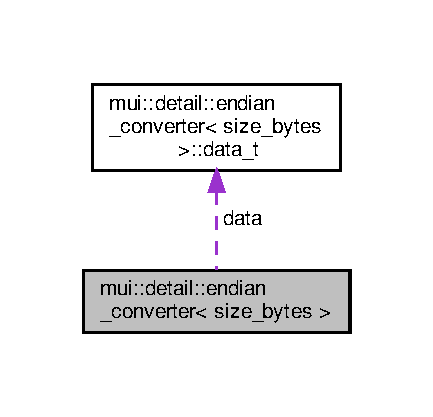
\includegraphics[width=208pt]{structmui_1_1detail_1_1endian__converter__coll__graph}
\end{center}
\end{figure}
\subsection*{Classes}
\begin{DoxyCompactItemize}
\item 
union \hyperlink{unionmui_1_1detail_1_1endian__converter_1_1data__t}{data\+\_\+t}
\end{DoxyCompactItemize}
\subsection*{Public Member Functions}
\begin{DoxyCompactItemize}
\item 
void \hyperlink{structmui_1_1detail_1_1endian__converter_aef400975d1bd9a4a376711697d03239a}{htobe} ()
\item 
void \hyperlink{structmui_1_1detail_1_1endian__converter_a944e222e219959cd2fea153cac688c0e}{betoh} ()
\item 
{\footnotesize template$<$$>$ }\\void \hyperlink{structmui_1_1detail_1_1endian__converter_aa1a6a5a85e932b4a8b7aee1eef711497}{htobe} ()
\item 
{\footnotesize template$<$$>$ }\\void \hyperlink{structmui_1_1detail_1_1endian__converter_ab0f14ea48f1d5a0d961a9a971f693c45}{betoh} ()
\item 
{\footnotesize template$<$$>$ }\\void \hyperlink{structmui_1_1detail_1_1endian__converter_ab2ccc8fea0e71d43406c46069642e97f}{htobe} ()
\item 
{\footnotesize template$<$$>$ }\\void \hyperlink{structmui_1_1detail_1_1endian__converter_a8d4f028749a475d3f22350ebf34c0499}{betoh} ()
\item 
{\footnotesize template$<$$>$ }\\void \hyperlink{structmui_1_1detail_1_1endian__converter_a08c71b98455a03a114f28872c6fda6e8}{htobe} ()
\item 
{\footnotesize template$<$$>$ }\\void \hyperlink{structmui_1_1detail_1_1endian__converter_a900f063b5f8fa85113653d43ae450aad}{betoh} ()
\end{DoxyCompactItemize}
\subsection*{Public Attributes}
\begin{DoxyCompactItemize}
\item 
\hyperlink{unionmui_1_1detail_1_1endian__converter_1_1data__t}{data\+\_\+t} \hyperlink{structmui_1_1detail_1_1endian__converter_a1e68df4966d4777253a3540405b4fd25}{data}
\end{DoxyCompactItemize}


\subsection{Member Function Documentation}
\mbox{\Hypertarget{structmui_1_1detail_1_1endian__converter_a944e222e219959cd2fea153cac688c0e}\label{structmui_1_1detail_1_1endian__converter_a944e222e219959cd2fea153cac688c0e}} 
\index{mui\+::detail\+::endian\+\_\+converter@{mui\+::detail\+::endian\+\_\+converter}!betoh@{betoh}}
\index{betoh@{betoh}!mui\+::detail\+::endian\+\_\+converter@{mui\+::detail\+::endian\+\_\+converter}}
\subsubsection{\texorpdfstring{betoh()}{betoh()}\hspace{0.1cm}{\footnotesize\ttfamily [1/4]}}
{\footnotesize\ttfamily template$<$size\+\_\+t size\+\_\+bytes$>$ \\
void \hyperlink{structmui_1_1detail_1_1endian__converter}{mui\+::detail\+::endian\+\_\+converter}$<$ size\+\_\+bytes $>$\+::betoh (\begin{DoxyParamCaption}{ }\end{DoxyParamCaption})}

\mbox{\Hypertarget{structmui_1_1detail_1_1endian__converter_ab0f14ea48f1d5a0d961a9a971f693c45}\label{structmui_1_1detail_1_1endian__converter_ab0f14ea48f1d5a0d961a9a971f693c45}} 
\index{mui\+::detail\+::endian\+\_\+converter@{mui\+::detail\+::endian\+\_\+converter}!betoh@{betoh}}
\index{betoh@{betoh}!mui\+::detail\+::endian\+\_\+converter@{mui\+::detail\+::endian\+\_\+converter}}
\subsubsection{\texorpdfstring{betoh()}{betoh()}\hspace{0.1cm}{\footnotesize\ttfamily [2/4]}}
{\footnotesize\ttfamily template$<$$>$ \\
void \hyperlink{structmui_1_1detail_1_1endian__converter}{mui\+::detail\+::endian\+\_\+converter}$<$ 2 $>$\+::betoh (\begin{DoxyParamCaption}{ }\end{DoxyParamCaption})\hspace{0.3cm}{\ttfamily [inline]}}

\mbox{\Hypertarget{structmui_1_1detail_1_1endian__converter_a8d4f028749a475d3f22350ebf34c0499}\label{structmui_1_1detail_1_1endian__converter_a8d4f028749a475d3f22350ebf34c0499}} 
\index{mui\+::detail\+::endian\+\_\+converter@{mui\+::detail\+::endian\+\_\+converter}!betoh@{betoh}}
\index{betoh@{betoh}!mui\+::detail\+::endian\+\_\+converter@{mui\+::detail\+::endian\+\_\+converter}}
\subsubsection{\texorpdfstring{betoh()}{betoh()}\hspace{0.1cm}{\footnotesize\ttfamily [3/4]}}
{\footnotesize\ttfamily template$<$$>$ \\
void \hyperlink{structmui_1_1detail_1_1endian__converter}{mui\+::detail\+::endian\+\_\+converter}$<$ 4 $>$\+::betoh (\begin{DoxyParamCaption}{ }\end{DoxyParamCaption})\hspace{0.3cm}{\ttfamily [inline]}}

\mbox{\Hypertarget{structmui_1_1detail_1_1endian__converter_a900f063b5f8fa85113653d43ae450aad}\label{structmui_1_1detail_1_1endian__converter_a900f063b5f8fa85113653d43ae450aad}} 
\index{mui\+::detail\+::endian\+\_\+converter@{mui\+::detail\+::endian\+\_\+converter}!betoh@{betoh}}
\index{betoh@{betoh}!mui\+::detail\+::endian\+\_\+converter@{mui\+::detail\+::endian\+\_\+converter}}
\subsubsection{\texorpdfstring{betoh()}{betoh()}\hspace{0.1cm}{\footnotesize\ttfamily [4/4]}}
{\footnotesize\ttfamily template$<$$>$ \\
void \hyperlink{structmui_1_1detail_1_1endian__converter}{mui\+::detail\+::endian\+\_\+converter}$<$ 8 $>$\+::betoh (\begin{DoxyParamCaption}{ }\end{DoxyParamCaption})\hspace{0.3cm}{\ttfamily [inline]}}

\mbox{\Hypertarget{structmui_1_1detail_1_1endian__converter_aef400975d1bd9a4a376711697d03239a}\label{structmui_1_1detail_1_1endian__converter_aef400975d1bd9a4a376711697d03239a}} 
\index{mui\+::detail\+::endian\+\_\+converter@{mui\+::detail\+::endian\+\_\+converter}!htobe@{htobe}}
\index{htobe@{htobe}!mui\+::detail\+::endian\+\_\+converter@{mui\+::detail\+::endian\+\_\+converter}}
\subsubsection{\texorpdfstring{htobe()}{htobe()}\hspace{0.1cm}{\footnotesize\ttfamily [1/4]}}
{\footnotesize\ttfamily template$<$size\+\_\+t size\+\_\+bytes$>$ \\
void \hyperlink{structmui_1_1detail_1_1endian__converter}{mui\+::detail\+::endian\+\_\+converter}$<$ size\+\_\+bytes $>$\+::htobe (\begin{DoxyParamCaption}{ }\end{DoxyParamCaption})}

\mbox{\Hypertarget{structmui_1_1detail_1_1endian__converter_aa1a6a5a85e932b4a8b7aee1eef711497}\label{structmui_1_1detail_1_1endian__converter_aa1a6a5a85e932b4a8b7aee1eef711497}} 
\index{mui\+::detail\+::endian\+\_\+converter@{mui\+::detail\+::endian\+\_\+converter}!htobe@{htobe}}
\index{htobe@{htobe}!mui\+::detail\+::endian\+\_\+converter@{mui\+::detail\+::endian\+\_\+converter}}
\subsubsection{\texorpdfstring{htobe()}{htobe()}\hspace{0.1cm}{\footnotesize\ttfamily [2/4]}}
{\footnotesize\ttfamily template$<$$>$ \\
void \hyperlink{structmui_1_1detail_1_1endian__converter}{mui\+::detail\+::endian\+\_\+converter}$<$ 2 $>$\+::htobe (\begin{DoxyParamCaption}{ }\end{DoxyParamCaption})\hspace{0.3cm}{\ttfamily [inline]}}

\mbox{\Hypertarget{structmui_1_1detail_1_1endian__converter_ab2ccc8fea0e71d43406c46069642e97f}\label{structmui_1_1detail_1_1endian__converter_ab2ccc8fea0e71d43406c46069642e97f}} 
\index{mui\+::detail\+::endian\+\_\+converter@{mui\+::detail\+::endian\+\_\+converter}!htobe@{htobe}}
\index{htobe@{htobe}!mui\+::detail\+::endian\+\_\+converter@{mui\+::detail\+::endian\+\_\+converter}}
\subsubsection{\texorpdfstring{htobe()}{htobe()}\hspace{0.1cm}{\footnotesize\ttfamily [3/4]}}
{\footnotesize\ttfamily template$<$$>$ \\
void \hyperlink{structmui_1_1detail_1_1endian__converter}{mui\+::detail\+::endian\+\_\+converter}$<$ 4 $>$\+::htobe (\begin{DoxyParamCaption}{ }\end{DoxyParamCaption})\hspace{0.3cm}{\ttfamily [inline]}}

\mbox{\Hypertarget{structmui_1_1detail_1_1endian__converter_a08c71b98455a03a114f28872c6fda6e8}\label{structmui_1_1detail_1_1endian__converter_a08c71b98455a03a114f28872c6fda6e8}} 
\index{mui\+::detail\+::endian\+\_\+converter@{mui\+::detail\+::endian\+\_\+converter}!htobe@{htobe}}
\index{htobe@{htobe}!mui\+::detail\+::endian\+\_\+converter@{mui\+::detail\+::endian\+\_\+converter}}
\subsubsection{\texorpdfstring{htobe()}{htobe()}\hspace{0.1cm}{\footnotesize\ttfamily [4/4]}}
{\footnotesize\ttfamily template$<$$>$ \\
void \hyperlink{structmui_1_1detail_1_1endian__converter}{mui\+::detail\+::endian\+\_\+converter}$<$ 8 $>$\+::htobe (\begin{DoxyParamCaption}{ }\end{DoxyParamCaption})\hspace{0.3cm}{\ttfamily [inline]}}



\subsection{Member Data Documentation}
\mbox{\Hypertarget{structmui_1_1detail_1_1endian__converter_a1e68df4966d4777253a3540405b4fd25}\label{structmui_1_1detail_1_1endian__converter_a1e68df4966d4777253a3540405b4fd25}} 
\index{mui\+::detail\+::endian\+\_\+converter@{mui\+::detail\+::endian\+\_\+converter}!data@{data}}
\index{data@{data}!mui\+::detail\+::endian\+\_\+converter@{mui\+::detail\+::endian\+\_\+converter}}
\subsubsection{\texorpdfstring{data}{data}}
{\footnotesize\ttfamily template$<$size\+\_\+t size\+\_\+bytes$>$ \\
\hyperlink{unionmui_1_1detail_1_1endian__converter_1_1data__t}{data\+\_\+t} \hyperlink{structmui_1_1detail_1_1endian__converter}{mui\+::detail\+::endian\+\_\+converter}$<$ size\+\_\+bytes $>$\+::data}



The documentation for this struct was generated from the following file\+:\begin{DoxyCompactItemize}
\item 
\hyperlink{endian__traits_8h}{endian\+\_\+traits.\+h}\end{DoxyCompactItemize}

\hypertarget{structmui_1_1endian__traits}{}\section{mui\+:\+:endian\+\_\+traits$<$ T, enable $>$ Struct Template Reference}
\label{structmui_1_1endian__traits}\index{mui\+::endian\+\_\+traits$<$ T, enable $>$@{mui\+::endian\+\_\+traits$<$ T, enable $>$}}


{\ttfamily \#include $<$endian\+\_\+traits.\+h$>$}



The documentation for this struct was generated from the following file\+:\begin{DoxyCompactItemize}
\item 
\hyperlink{endian__traits_8h}{endian\+\_\+traits.\+h}\end{DoxyCompactItemize}

\hypertarget{structmui_1_1endian__traits_3_01_t_00_01typename_01std_1_1enable__if_3_01std_1_1is__floating__po2204fe17b69811056c26bb26c4197e1a}{}\section{mui\+:\+:endian\+\_\+traits$<$ T, typename std\+:\+:enable\+\_\+if$<$ std\+:\+:is\+\_\+floating\+\_\+point$<$ T $>$\+:\+:value $>$\+:\+:type $>$ Struct Template Reference}
\label{structmui_1_1endian__traits_3_01_t_00_01typename_01std_1_1enable__if_3_01std_1_1is__floating__po2204fe17b69811056c26bb26c4197e1a}\index{mui\+::endian\+\_\+traits$<$ T, typename std\+::enable\+\_\+if$<$ std\+::is\+\_\+floating\+\_\+point$<$ T $>$\+::value $>$\+::type $>$@{mui\+::endian\+\_\+traits$<$ T, typename std\+::enable\+\_\+if$<$ std\+::is\+\_\+floating\+\_\+point$<$ T $>$\+::value $>$\+::type $>$}}


{\ttfamily \#include $<$endian\+\_\+traits.\+h$>$}

\subsection*{Static Public Attributes}
\begin{DoxyCompactItemize}
\item 
static constexpr bool \hyperlink{structmui_1_1endian__traits_3_01_t_00_01typename_01std_1_1enable__if_3_01std_1_1is__floating__po2204fe17b69811056c26bb26c4197e1a_a891095e1ac8c993814c1adaaee9fc15d}{convert} = M\+U\+I\+\_\+\+C\+O\+N\+V\+E\+R\+T\+\_\+\+F\+L\+O\+AT
\end{DoxyCompactItemize}


\subsection{Member Data Documentation}
\mbox{\Hypertarget{structmui_1_1endian__traits_3_01_t_00_01typename_01std_1_1enable__if_3_01std_1_1is__floating__po2204fe17b69811056c26bb26c4197e1a_a891095e1ac8c993814c1adaaee9fc15d}\label{structmui_1_1endian__traits_3_01_t_00_01typename_01std_1_1enable__if_3_01std_1_1is__floating__po2204fe17b69811056c26bb26c4197e1a_a891095e1ac8c993814c1adaaee9fc15d}} 
\index{mui\+::endian\+\_\+traits$<$ T, typename std\+::enable\+\_\+if$<$ std\+::is\+\_\+floating\+\_\+point$<$ T $>$\+::value $>$\+::type $>$@{mui\+::endian\+\_\+traits$<$ T, typename std\+::enable\+\_\+if$<$ std\+::is\+\_\+floating\+\_\+point$<$ T $>$\+::value $>$\+::type $>$}!convert@{convert}}
\index{convert@{convert}!mui\+::endian\+\_\+traits$<$ T, typename std\+::enable\+\_\+if$<$ std\+::is\+\_\+floating\+\_\+point$<$ T $>$\+::value $>$\+::type $>$@{mui\+::endian\+\_\+traits$<$ T, typename std\+::enable\+\_\+if$<$ std\+::is\+\_\+floating\+\_\+point$<$ T $>$\+::value $>$\+::type $>$}}
\subsubsection{\texorpdfstring{convert}{convert}}
{\footnotesize\ttfamily template$<$typename T $>$ \\
constexpr bool \hyperlink{structmui_1_1endian__traits}{mui\+::endian\+\_\+traits}$<$ T, typename std\+::enable\+\_\+if$<$ std\+::is\+\_\+floating\+\_\+point$<$ T $>$\+::value $>$\+::type $>$\+::convert = M\+U\+I\+\_\+\+C\+O\+N\+V\+E\+R\+T\+\_\+\+F\+L\+O\+AT\hspace{0.3cm}{\ttfamily [static]}}



The documentation for this struct was generated from the following file\+:\begin{DoxyCompactItemize}
\item 
\hyperlink{endian__traits_8h}{endian\+\_\+traits.\+h}\end{DoxyCompactItemize}

\hypertarget{structmui_1_1endian__traits_3_01_t_00_01typename_01std_1_1enable__if_3_01std_1_1is__integral_3_017f2a9fc75456eff64bb43276e6e0ef4}{}\section{mui\+:\+:endian\+\_\+traits$<$ T, typename std\+:\+:enable\+\_\+if$<$ std\+:\+:is\+\_\+integral$<$ T $>$\+:\+:value $>$\+:\+:type $>$ Struct Template Reference}
\label{structmui_1_1endian__traits_3_01_t_00_01typename_01std_1_1enable__if_3_01std_1_1is__integral_3_017f2a9fc75456eff64bb43276e6e0ef4}\index{mui\+::endian\+\_\+traits$<$ T, typename std\+::enable\+\_\+if$<$ std\+::is\+\_\+integral$<$ T $>$\+::value $>$\+::type $>$@{mui\+::endian\+\_\+traits$<$ T, typename std\+::enable\+\_\+if$<$ std\+::is\+\_\+integral$<$ T $>$\+::value $>$\+::type $>$}}


{\ttfamily \#include $<$endian\+\_\+traits.\+h$>$}

\subsection*{Static Public Attributes}
\begin{DoxyCompactItemize}
\item 
static constexpr bool \hyperlink{structmui_1_1endian__traits_3_01_t_00_01typename_01std_1_1enable__if_3_01std_1_1is__integral_3_017f2a9fc75456eff64bb43276e6e0ef4_a0e63e3bb67c6b38aa88e03750bd68548}{convert} = (sizeof(T) $>$ 1) \&\& M\+U\+I\+\_\+\+C\+O\+N\+V\+E\+R\+T\+\_\+\+I\+NT
\end{DoxyCompactItemize}


\subsection{Member Data Documentation}
\mbox{\Hypertarget{structmui_1_1endian__traits_3_01_t_00_01typename_01std_1_1enable__if_3_01std_1_1is__integral_3_017f2a9fc75456eff64bb43276e6e0ef4_a0e63e3bb67c6b38aa88e03750bd68548}\label{structmui_1_1endian__traits_3_01_t_00_01typename_01std_1_1enable__if_3_01std_1_1is__integral_3_017f2a9fc75456eff64bb43276e6e0ef4_a0e63e3bb67c6b38aa88e03750bd68548}} 
\index{mui\+::endian\+\_\+traits$<$ T, typename std\+::enable\+\_\+if$<$ std\+::is\+\_\+integral$<$ T $>$\+::value $>$\+::type $>$@{mui\+::endian\+\_\+traits$<$ T, typename std\+::enable\+\_\+if$<$ std\+::is\+\_\+integral$<$ T $>$\+::value $>$\+::type $>$}!convert@{convert}}
\index{convert@{convert}!mui\+::endian\+\_\+traits$<$ T, typename std\+::enable\+\_\+if$<$ std\+::is\+\_\+integral$<$ T $>$\+::value $>$\+::type $>$@{mui\+::endian\+\_\+traits$<$ T, typename std\+::enable\+\_\+if$<$ std\+::is\+\_\+integral$<$ T $>$\+::value $>$\+::type $>$}}
\subsubsection{\texorpdfstring{convert}{convert}}
{\footnotesize\ttfamily template$<$typename T $>$ \\
constexpr bool \hyperlink{structmui_1_1endian__traits}{mui\+::endian\+\_\+traits}$<$ T, typename std\+::enable\+\_\+if$<$ std\+::is\+\_\+integral$<$ T $>$\+::value $>$\+::type $>$\+::convert = (sizeof(T) $>$ 1) \&\& M\+U\+I\+\_\+\+C\+O\+N\+V\+E\+R\+T\+\_\+\+I\+NT\hspace{0.3cm}{\ttfamily [static]}}



The documentation for this struct was generated from the following file\+:\begin{DoxyCompactItemize}
\item 
\hyperlink{endian__traits_8h}{endian\+\_\+traits.\+h}\end{DoxyCompactItemize}

\hypertarget{structmui_1_1exception__abort}{}\section{mui\+:\+:exception\+\_\+abort Struct Reference}
\label{structmui_1_1exception__abort}\index{mui\+::exception\+\_\+abort@{mui\+::exception\+\_\+abort}}


{\ttfamily \#include $<$exception.\+h$>$}

\subsection*{Public Member Functions}
\begin{DoxyCompactItemize}
\item 
\hyperlink{structmui_1_1exception__abort_a6ae2cb4096147601424fbb05463421cc}{exception\+\_\+abort} (const std\+::exception \&except)
\end{DoxyCompactItemize}


\subsection{Constructor \& Destructor Documentation}
\mbox{\Hypertarget{structmui_1_1exception__abort_a6ae2cb4096147601424fbb05463421cc}\label{structmui_1_1exception__abort_a6ae2cb4096147601424fbb05463421cc}} 
\index{mui\+::exception\+\_\+abort@{mui\+::exception\+\_\+abort}!exception\+\_\+abort@{exception\+\_\+abort}}
\index{exception\+\_\+abort@{exception\+\_\+abort}!mui\+::exception\+\_\+abort@{mui\+::exception\+\_\+abort}}
\subsubsection{\texorpdfstring{exception\+\_\+abort()}{exception\_abort()}}
{\footnotesize\ttfamily mui\+::exception\+\_\+abort\+::exception\+\_\+abort (\begin{DoxyParamCaption}\item[{const std\+::exception \&}]{except }\end{DoxyParamCaption})\hspace{0.3cm}{\ttfamily [inline]}}



The documentation for this struct was generated from the following file\+:\begin{DoxyCompactItemize}
\item 
\hyperlink{exception_8h}{exception.\+h}\end{DoxyCompactItemize}

\hypertarget{structmui_1_1exception__segv}{}\section{mui\+:\+:exception\+\_\+segv Struct Reference}
\label{structmui_1_1exception__segv}\index{mui\+::exception\+\_\+segv@{mui\+::exception\+\_\+segv}}


{\ttfamily \#include $<$exception.\+h$>$}

\subsection*{Public Member Functions}
\begin{DoxyCompactItemize}
\item 
\hyperlink{structmui_1_1exception__segv_abd398976a6fcd156262e033c274b72b4}{exception\+\_\+segv} ()
\item 
{\footnotesize template$<$typename H\+E\+AD , typename ... T\+A\+IL$>$ }\\\hyperlink{structmui_1_1exception__segv_aecea0ce4316060d83687d8b7c053dfd3}{exception\+\_\+segv} (H\+E\+AD const \&head, T\+A\+IL const \&... tail)
\item 
{\footnotesize template$<$typename H\+E\+AD , typename ... T\+A\+IL$>$ }\\void \hyperlink{structmui_1_1exception__segv_a2a0e173d21952400fa3aab0ec418338c}{handle} (H\+E\+AD const \&head, T\+A\+IL const \&... tail)
\item 
void \hyperlink{structmui_1_1exception__segv_a9a4e64bfd3ff46807c92706be20ce3fa}{handle} (void)
\end{DoxyCompactItemize}


\subsection{Constructor \& Destructor Documentation}
\mbox{\Hypertarget{structmui_1_1exception__segv_abd398976a6fcd156262e033c274b72b4}\label{structmui_1_1exception__segv_abd398976a6fcd156262e033c274b72b4}} 
\index{mui\+::exception\+\_\+segv@{mui\+::exception\+\_\+segv}!exception\+\_\+segv@{exception\+\_\+segv}}
\index{exception\+\_\+segv@{exception\+\_\+segv}!mui\+::exception\+\_\+segv@{mui\+::exception\+\_\+segv}}
\subsubsection{\texorpdfstring{exception\+\_\+segv()}{exception\_segv()}\hspace{0.1cm}{\footnotesize\ttfamily [1/2]}}
{\footnotesize\ttfamily mui\+::exception\+\_\+segv\+::exception\+\_\+segv (\begin{DoxyParamCaption}{ }\end{DoxyParamCaption})\hspace{0.3cm}{\ttfamily [inline]}, {\ttfamily [explicit]}}

\mbox{\Hypertarget{structmui_1_1exception__segv_aecea0ce4316060d83687d8b7c053dfd3}\label{structmui_1_1exception__segv_aecea0ce4316060d83687d8b7c053dfd3}} 
\index{mui\+::exception\+\_\+segv@{mui\+::exception\+\_\+segv}!exception\+\_\+segv@{exception\+\_\+segv}}
\index{exception\+\_\+segv@{exception\+\_\+segv}!mui\+::exception\+\_\+segv@{mui\+::exception\+\_\+segv}}
\subsubsection{\texorpdfstring{exception\+\_\+segv()}{exception\_segv()}\hspace{0.1cm}{\footnotesize\ttfamily [2/2]}}
{\footnotesize\ttfamily template$<$typename H\+E\+AD , typename ... T\+A\+IL$>$ \\
mui\+::exception\+\_\+segv\+::exception\+\_\+segv (\begin{DoxyParamCaption}\item[{H\+E\+AD const \&}]{head,  }\item[{T\+A\+IL const \&...}]{tail }\end{DoxyParamCaption})\hspace{0.3cm}{\ttfamily [inline]}}



\subsection{Member Function Documentation}
\mbox{\Hypertarget{structmui_1_1exception__segv_a2a0e173d21952400fa3aab0ec418338c}\label{structmui_1_1exception__segv_a2a0e173d21952400fa3aab0ec418338c}} 
\index{mui\+::exception\+\_\+segv@{mui\+::exception\+\_\+segv}!handle@{handle}}
\index{handle@{handle}!mui\+::exception\+\_\+segv@{mui\+::exception\+\_\+segv}}
\subsubsection{\texorpdfstring{handle()}{handle()}\hspace{0.1cm}{\footnotesize\ttfamily [1/2]}}
{\footnotesize\ttfamily template$<$typename H\+E\+AD , typename ... T\+A\+IL$>$ \\
void mui\+::exception\+\_\+segv\+::handle (\begin{DoxyParamCaption}\item[{H\+E\+AD const \&}]{head,  }\item[{T\+A\+IL const \&...}]{tail }\end{DoxyParamCaption})\hspace{0.3cm}{\ttfamily [inline]}}

\mbox{\Hypertarget{structmui_1_1exception__segv_a9a4e64bfd3ff46807c92706be20ce3fa}\label{structmui_1_1exception__segv_a9a4e64bfd3ff46807c92706be20ce3fa}} 
\index{mui\+::exception\+\_\+segv@{mui\+::exception\+\_\+segv}!handle@{handle}}
\index{handle@{handle}!mui\+::exception\+\_\+segv@{mui\+::exception\+\_\+segv}}
\subsubsection{\texorpdfstring{handle()}{handle()}\hspace{0.1cm}{\footnotesize\ttfamily [2/2]}}
{\footnotesize\ttfamily void mui\+::exception\+\_\+segv\+::handle (\begin{DoxyParamCaption}\item[{void}]{ }\end{DoxyParamCaption})\hspace{0.3cm}{\ttfamily [inline]}}



The documentation for this struct was generated from the following file\+:\begin{DoxyCompactItemize}
\item 
\hyperlink{exception_8h}{exception.\+h}\end{DoxyCompactItemize}

\hypertarget{structmui_1_1exception__throw}{}\section{mui\+:\+:exception\+\_\+throw Struct Reference}
\label{structmui_1_1exception__throw}\index{mui\+::exception\+\_\+throw@{mui\+::exception\+\_\+throw}}


{\ttfamily \#include $<$exception.\+h$>$}

\subsection*{Public Member Functions}
\begin{DoxyCompactItemize}
\item 
\hyperlink{structmui_1_1exception__throw_a611d5d1ba748145c3eed906040304dd7}{exception\+\_\+throw} (const std\+::exception \&)
\end{DoxyCompactItemize}


\subsection{Constructor \& Destructor Documentation}
\mbox{\Hypertarget{structmui_1_1exception__throw_a611d5d1ba748145c3eed906040304dd7}\label{structmui_1_1exception__throw_a611d5d1ba748145c3eed906040304dd7}} 
\index{mui\+::exception\+\_\+throw@{mui\+::exception\+\_\+throw}!exception\+\_\+throw@{exception\+\_\+throw}}
\index{exception\+\_\+throw@{exception\+\_\+throw}!mui\+::exception\+\_\+throw@{mui\+::exception\+\_\+throw}}
\subsubsection{\texorpdfstring{exception\+\_\+throw()}{exception\_throw()}}
{\footnotesize\ttfamily mui\+::exception\+\_\+throw\+::exception\+\_\+throw (\begin{DoxyParamCaption}\item[{const std\+::exception \&}]{ }\end{DoxyParamCaption})\hspace{0.3cm}{\ttfamily [inline]}}



The documentation for this struct was generated from the following file\+:\begin{DoxyCompactItemize}
\item 
\hyperlink{exception_8h}{exception.\+h}\end{DoxyCompactItemize}

\hypertarget{classmui4py_1_1geometry_1_1_geometry}{}\section{mui4py.\+geometry.\+Geometry Class Reference}
\label{classmui4py_1_1geometry_1_1_geometry}\index{mui4py.\+geometry.\+Geometry@{mui4py.\+geometry.\+Geometry}}


Inheritance diagram for mui4py.\+geometry.\+Geometry\+:
\nopagebreak
\begin{figure}[H]
\begin{center}
\leavevmode
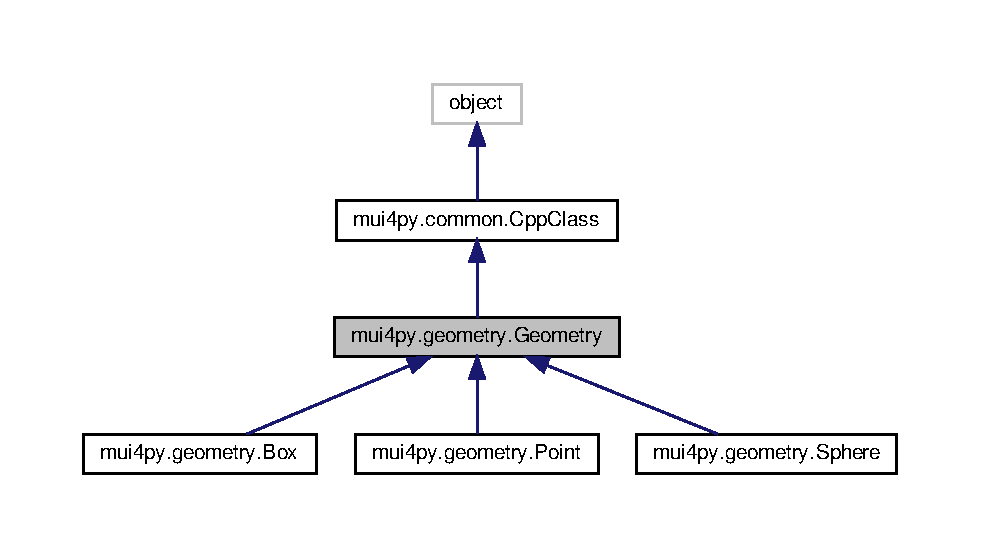
\includegraphics[width=350pt]{classmui4py_1_1geometry_1_1_geometry__inherit__graph}
\end{center}
\end{figure}


Collaboration diagram for mui4py.\+geometry.\+Geometry\+:
\nopagebreak
\begin{figure}[H]
\begin{center}
\leavevmode
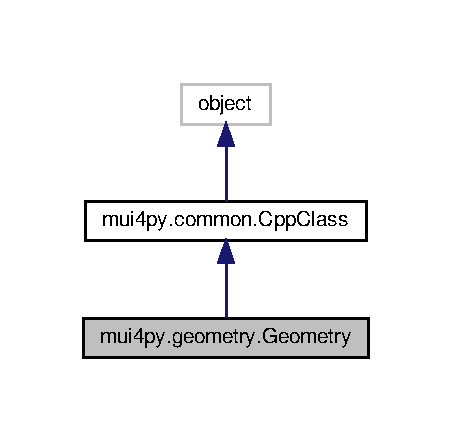
\includegraphics[width=217pt]{classmui4py_1_1geometry_1_1_geometry__coll__graph}
\end{center}
\end{figure}
\subsection*{Public Member Functions}
\begin{DoxyCompactItemize}
\item 
def \hyperlink{classmui4py_1_1geometry_1_1_geometry_ab4442f9d6c919cd2822b63b86d3529d6}{\+\_\+\+\_\+init\+\_\+\+\_\+} (self, \hyperlink{classmui4py_1_1common_1_1_cpp_class_a29797823c6e21f22bba24ee7d35ef31d}{args}=(), \hyperlink{classmui4py_1_1common_1_1_cpp_class_af43879f06f07b1abf0d08e30c5ead46f}{kwargs}=\{\})
\item 
def \hyperlink{classmui4py_1_1geometry_1_1_geometry_ad32b8e1fdc5dbc35909ff03f4787df8e}{bbox} (self)
\end{DoxyCompactItemize}
\subsection*{Public Attributes}
\begin{DoxyCompactItemize}
\item 
\hyperlink{classmui4py_1_1geometry_1_1_geometry_a953a13572dab2da3a02d9ce4ff010139}{namespace}
\end{DoxyCompactItemize}


\subsection{Constructor \& Destructor Documentation}
\mbox{\Hypertarget{classmui4py_1_1geometry_1_1_geometry_ab4442f9d6c919cd2822b63b86d3529d6}\label{classmui4py_1_1geometry_1_1_geometry_ab4442f9d6c919cd2822b63b86d3529d6}} 
\index{mui4py\+::geometry\+::\+Geometry@{mui4py\+::geometry\+::\+Geometry}!\+\_\+\+\_\+init\+\_\+\+\_\+@{\+\_\+\+\_\+init\+\_\+\+\_\+}}
\index{\+\_\+\+\_\+init\+\_\+\+\_\+@{\+\_\+\+\_\+init\+\_\+\+\_\+}!mui4py\+::geometry\+::\+Geometry@{mui4py\+::geometry\+::\+Geometry}}
\subsubsection{\texorpdfstring{\+\_\+\+\_\+init\+\_\+\+\_\+()}{\_\_init\_\_()}}
{\footnotesize\ttfamily def mui4py.\+geometry.\+Geometry.\+\_\+\+\_\+init\+\_\+\+\_\+ (\begin{DoxyParamCaption}\item[{}]{self,  }\item[{}]{args = {\ttfamily ()},  }\item[{}]{kwargs = {\ttfamily \{\}} }\end{DoxyParamCaption})}



\subsection{Member Function Documentation}
\mbox{\Hypertarget{classmui4py_1_1geometry_1_1_geometry_ad32b8e1fdc5dbc35909ff03f4787df8e}\label{classmui4py_1_1geometry_1_1_geometry_ad32b8e1fdc5dbc35909ff03f4787df8e}} 
\index{mui4py\+::geometry\+::\+Geometry@{mui4py\+::geometry\+::\+Geometry}!bbox@{bbox}}
\index{bbox@{bbox}!mui4py\+::geometry\+::\+Geometry@{mui4py\+::geometry\+::\+Geometry}}
\subsubsection{\texorpdfstring{bbox()}{bbox()}}
{\footnotesize\ttfamily def mui4py.\+geometry.\+Geometry.\+bbox (\begin{DoxyParamCaption}\item[{}]{self }\end{DoxyParamCaption})}



\subsection{Member Data Documentation}
\mbox{\Hypertarget{classmui4py_1_1geometry_1_1_geometry_a953a13572dab2da3a02d9ce4ff010139}\label{classmui4py_1_1geometry_1_1_geometry_a953a13572dab2da3a02d9ce4ff010139}} 
\index{mui4py\+::geometry\+::\+Geometry@{mui4py\+::geometry\+::\+Geometry}!namespace@{namespace}}
\index{namespace@{namespace}!mui4py\+::geometry\+::\+Geometry@{mui4py\+::geometry\+::\+Geometry}}
\subsubsection{\texorpdfstring{namespace}{namespace}}
{\footnotesize\ttfamily mui4py.\+geometry.\+Geometry.\+namespace}



The documentation for this class was generated from the following file\+:\begin{DoxyCompactItemize}
\item 
wrappers/\+Python/mui4py/\hyperlink{geometry_8py}{geometry.\+py}\end{DoxyCompactItemize}

\hypertarget{classmui_1_1iitr__stream}{}\section{mui\+:\+:iitr\+\_\+stream$<$ Const\+Input\+Iterator $>$ Class Template Reference}
\label{classmui_1_1iitr__stream}\index{mui\+::iitr\+\_\+stream$<$ Const\+Input\+Iterator $>$@{mui\+::iitr\+\_\+stream$<$ Const\+Input\+Iterator $>$}}


{\ttfamily \#include $<$stream.\+h$>$}



Inheritance diagram for mui\+:\+:iitr\+\_\+stream$<$ Const\+Input\+Iterator $>$\+:
\nopagebreak
\begin{figure}[H]
\begin{center}
\leavevmode
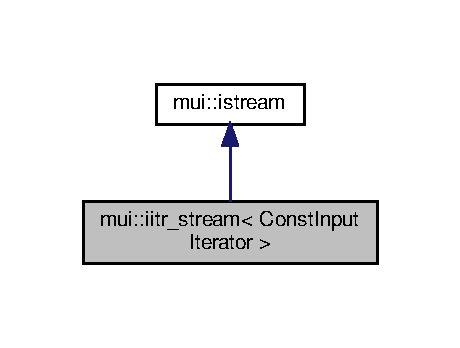
\includegraphics[width=221pt]{classmui_1_1iitr__stream__inherit__graph}
\end{center}
\end{figure}


Collaboration diagram for mui\+:\+:iitr\+\_\+stream$<$ Const\+Input\+Iterator $>$\+:
\nopagebreak
\begin{figure}[H]
\begin{center}
\leavevmode
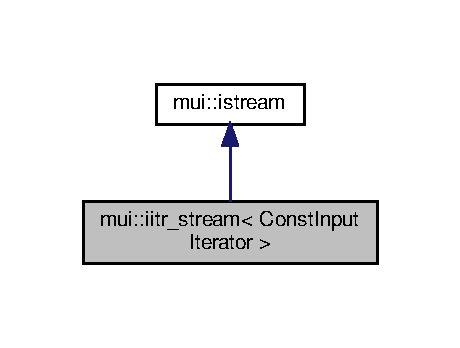
\includegraphics[width=221pt]{classmui_1_1iitr__stream__coll__graph}
\end{center}
\end{figure}
\subsection*{Public Member Functions}
\begin{DoxyCompactItemize}
\item 
\hyperlink{classmui_1_1iitr__stream_a63616e1aa49e6c9393041ad41ee46459}{iitr\+\_\+stream} (const \hyperlink{classmui_1_1iitr__stream}{iitr\+\_\+stream} \&)=default
\item 
\hyperlink{classmui_1_1iitr__stream_a8989d81db9c1bf9736d7e00ca14dc80d}{iitr\+\_\+stream} (Const\+Input\+Iterator \hyperlink{bin_8h_adaedeb4494f60b41fe2e306a04764402}{cur\+\_\+})
\item 
\hyperlink{classmui_1_1iitr__stream_a129cf88483da2a1fc727aae04cb317d9}{$\sim$iitr\+\_\+stream} ()
\item 
void \hyperlink{classmui_1_1iitr__stream_aa39fd880d0a4ec821775a86c0d7bc2ce}{read} (char $\ast$ptr, std\+::size\+\_\+t sz)
\item 
Const\+Input\+Iterator \hyperlink{classmui_1_1iitr__stream_ab4f7f7a6e33eeb69b38d83b048dc9875}{current} () const
\end{DoxyCompactItemize}


\subsection{Constructor \& Destructor Documentation}
\mbox{\Hypertarget{classmui_1_1iitr__stream_a63616e1aa49e6c9393041ad41ee46459}\label{classmui_1_1iitr__stream_a63616e1aa49e6c9393041ad41ee46459}} 
\index{mui\+::iitr\+\_\+stream@{mui\+::iitr\+\_\+stream}!iitr\+\_\+stream@{iitr\+\_\+stream}}
\index{iitr\+\_\+stream@{iitr\+\_\+stream}!mui\+::iitr\+\_\+stream@{mui\+::iitr\+\_\+stream}}
\subsubsection{\texorpdfstring{iitr\+\_\+stream()}{iitr\_stream()}\hspace{0.1cm}{\footnotesize\ttfamily [1/2]}}
{\footnotesize\ttfamily template$<$typename Const\+Input\+Iterator $>$ \\
\hyperlink{classmui_1_1iitr__stream}{mui\+::iitr\+\_\+stream}$<$ Const\+Input\+Iterator $>$\+::\hyperlink{classmui_1_1iitr__stream}{iitr\+\_\+stream} (\begin{DoxyParamCaption}\item[{const \hyperlink{classmui_1_1iitr__stream}{iitr\+\_\+stream}$<$ Const\+Input\+Iterator $>$ \&}]{ }\end{DoxyParamCaption})\hspace{0.3cm}{\ttfamily [default]}}

\mbox{\Hypertarget{classmui_1_1iitr__stream_a8989d81db9c1bf9736d7e00ca14dc80d}\label{classmui_1_1iitr__stream_a8989d81db9c1bf9736d7e00ca14dc80d}} 
\index{mui\+::iitr\+\_\+stream@{mui\+::iitr\+\_\+stream}!iitr\+\_\+stream@{iitr\+\_\+stream}}
\index{iitr\+\_\+stream@{iitr\+\_\+stream}!mui\+::iitr\+\_\+stream@{mui\+::iitr\+\_\+stream}}
\subsubsection{\texorpdfstring{iitr\+\_\+stream()}{iitr\_stream()}\hspace{0.1cm}{\footnotesize\ttfamily [2/2]}}
{\footnotesize\ttfamily template$<$typename Const\+Input\+Iterator $>$ \\
\hyperlink{classmui_1_1iitr__stream}{mui\+::iitr\+\_\+stream}$<$ Const\+Input\+Iterator $>$\+::\hyperlink{classmui_1_1iitr__stream}{iitr\+\_\+stream} (\begin{DoxyParamCaption}\item[{Const\+Input\+Iterator}]{cur\+\_\+ }\end{DoxyParamCaption})\hspace{0.3cm}{\ttfamily [inline]}}

\mbox{\Hypertarget{classmui_1_1iitr__stream_a129cf88483da2a1fc727aae04cb317d9}\label{classmui_1_1iitr__stream_a129cf88483da2a1fc727aae04cb317d9}} 
\index{mui\+::iitr\+\_\+stream@{mui\+::iitr\+\_\+stream}!````~iitr\+\_\+stream@{$\sim$iitr\+\_\+stream}}
\index{````~iitr\+\_\+stream@{$\sim$iitr\+\_\+stream}!mui\+::iitr\+\_\+stream@{mui\+::iitr\+\_\+stream}}
\subsubsection{\texorpdfstring{$\sim$iitr\+\_\+stream()}{~iitr\_stream()}}
{\footnotesize\ttfamily template$<$typename Const\+Input\+Iterator $>$ \\
\hyperlink{classmui_1_1iitr__stream}{mui\+::iitr\+\_\+stream}$<$ Const\+Input\+Iterator $>$\+::$\sim$\hyperlink{classmui_1_1iitr__stream}{iitr\+\_\+stream} (\begin{DoxyParamCaption}{ }\end{DoxyParamCaption})\hspace{0.3cm}{\ttfamily [inline]}}



\subsection{Member Function Documentation}
\mbox{\Hypertarget{classmui_1_1iitr__stream_ab4f7f7a6e33eeb69b38d83b048dc9875}\label{classmui_1_1iitr__stream_ab4f7f7a6e33eeb69b38d83b048dc9875}} 
\index{mui\+::iitr\+\_\+stream@{mui\+::iitr\+\_\+stream}!current@{current}}
\index{current@{current}!mui\+::iitr\+\_\+stream@{mui\+::iitr\+\_\+stream}}
\subsubsection{\texorpdfstring{current()}{current()}}
{\footnotesize\ttfamily template$<$typename Const\+Input\+Iterator $>$ \\
Const\+Input\+Iterator \hyperlink{classmui_1_1iitr__stream}{mui\+::iitr\+\_\+stream}$<$ Const\+Input\+Iterator $>$\+::current (\begin{DoxyParamCaption}{ }\end{DoxyParamCaption}) const\hspace{0.3cm}{\ttfamily [inline]}}

\mbox{\Hypertarget{classmui_1_1iitr__stream_aa39fd880d0a4ec821775a86c0d7bc2ce}\label{classmui_1_1iitr__stream_aa39fd880d0a4ec821775a86c0d7bc2ce}} 
\index{mui\+::iitr\+\_\+stream@{mui\+::iitr\+\_\+stream}!read@{read}}
\index{read@{read}!mui\+::iitr\+\_\+stream@{mui\+::iitr\+\_\+stream}}
\subsubsection{\texorpdfstring{read()}{read()}}
{\footnotesize\ttfamily template$<$typename Const\+Input\+Iterator $>$ \\
void \hyperlink{classmui_1_1iitr__stream}{mui\+::iitr\+\_\+stream}$<$ Const\+Input\+Iterator $>$\+::read (\begin{DoxyParamCaption}\item[{char $\ast$}]{ptr,  }\item[{std\+::size\+\_\+t}]{sz }\end{DoxyParamCaption})\hspace{0.3cm}{\ttfamily [inline]}, {\ttfamily [virtual]}}



Implements \hyperlink{classmui_1_1istream_a275ecbe530bf67df5978be288897ab45}{mui\+::istream}.



The documentation for this class was generated from the following file\+:\begin{DoxyCompactItemize}
\item 
\hyperlink{stream_8h}{stream.\+h}\end{DoxyCompactItemize}

\hypertarget{structmui_1_1index__iterator}{}\section{mui\+:\+:index\+\_\+iterator$<$ V, A\+R\+R\+AY $>$ Struct Template Reference}
\label{structmui_1_1index__iterator}\index{mui\+::index\+\_\+iterator$<$ V, A\+R\+R\+A\+Y $>$@{mui\+::index\+\_\+iterator$<$ V, A\+R\+R\+A\+Y $>$}}


{\ttfamily \#include $<$virtual\+\_\+container.\+h$>$}



Inheritance diagram for mui\+:\+:index\+\_\+iterator$<$ V, A\+R\+R\+AY $>$\+:
\nopagebreak
\begin{figure}[H]
\begin{center}
\leavevmode
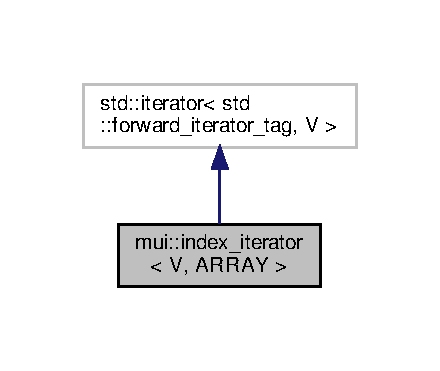
\includegraphics[width=211pt]{structmui_1_1index__iterator__inherit__graph}
\end{center}
\end{figure}


Collaboration diagram for mui\+:\+:index\+\_\+iterator$<$ V, A\+R\+R\+AY $>$\+:
\nopagebreak
\begin{figure}[H]
\begin{center}
\leavevmode
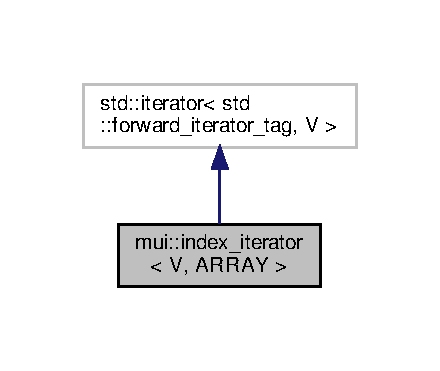
\includegraphics[width=211pt]{structmui_1_1index__iterator__coll__graph}
\end{center}
\end{figure}
\subsection*{Public Types}
\begin{DoxyCompactItemize}
\item 
typedef std\+::iterator$<$ std\+::forward\+\_\+iterator\+\_\+tag, V $>$ \hyperlink{structmui_1_1index__iterator_aceb32ff6af026ed8662f9fb30ea5cbe7}{iterator}
\item 
typedef iterator\+::iterator\+\_\+category \hyperlink{structmui_1_1index__iterator_a3a8f9b635405aaa0a076020be25cbf0b}{iterator\+\_\+category}
\item 
typedef iterator\+::value\+\_\+type \hyperlink{structmui_1_1index__iterator_a795af944e7eb34f4842a7f5d138fe186}{value\+\_\+type}
\item 
typedef iterator\+::difference\+\_\+type \hyperlink{structmui_1_1index__iterator_a1c78c601f90f622d37e36255c6e7260a}{difference\+\_\+type}
\item 
typedef iterator\+::pointer \hyperlink{structmui_1_1index__iterator_afbdc05d0a9403f2fb4002373c06dce97}{pointer}
\item 
typedef iterator\+::reference \hyperlink{structmui_1_1index__iterator_a3854dd112d5ca1a649babb0357e02394}{reference}
\end{DoxyCompactItemize}
\subsection*{Public Member Functions}
\begin{DoxyCompactItemize}
\item 
\hyperlink{structmui_1_1index__iterator_a974125f59982128660e17777a3b6cea8}{index\+\_\+iterator} (A\+R\+R\+AY \&array, std\+::size\+\_\+t index=0)
\item 
\hyperlink{structmui_1_1index__iterator_aef7a1a21afb42127dff73b2ebcb5c0a7}{index\+\_\+iterator} ()=default
\item 
\hyperlink{structmui_1_1index__iterator_ac51630f186471fbc8c55320e58b34439}{index\+\_\+iterator} (const \hyperlink{structmui_1_1index__iterator}{index\+\_\+iterator} \&)=default
\item 
\hyperlink{structmui_1_1index__iterator}{index\+\_\+iterator} \& \hyperlink{structmui_1_1index__iterator_aa86f191c1d319200d0aad177bf11d49a}{operator=} (const \hyperlink{structmui_1_1index__iterator}{index\+\_\+iterator} \&)=default
\item 
\hyperlink{structmui_1_1index__iterator_a795af944e7eb34f4842a7f5d138fe186}{value\+\_\+type} \hyperlink{structmui_1_1index__iterator_a8a9a41e163764c4e4a72a8e06f4835be}{operator$\ast$} () const
\item 
\hyperlink{structmui_1_1index__iterator_a3854dd112d5ca1a649babb0357e02394}{reference} \hyperlink{structmui_1_1index__iterator_a967bee24f2b395b2a25dc76f9d22aacb}{operator$\ast$} ()
\item 
const \hyperlink{structmui_1_1index__iterator_afbdc05d0a9403f2fb4002373c06dce97}{pointer} \hyperlink{structmui_1_1index__iterator_abe41aeb655f2be324323b8b445652abc}{operator-\/$>$} () const
\item 
\hyperlink{structmui_1_1index__iterator_afbdc05d0a9403f2fb4002373c06dce97}{pointer} \hyperlink{structmui_1_1index__iterator_ac34c72a3ac62e28434a5cd1f4e4d0427}{operator-\/$>$} ()
\item 
\hyperlink{structmui_1_1index__iterator}{index\+\_\+iterator} \& \hyperlink{structmui_1_1index__iterator_aaf0cc8e107e38388a15cf807b8f682fa}{operator++} ()
\item 
\hyperlink{structmui_1_1index__iterator}{index\+\_\+iterator} \hyperlink{structmui_1_1index__iterator_a7d8d2fecca6cf02b42a6de076cc766ea}{operator++} (int)
\item 
bool \hyperlink{structmui_1_1index__iterator_a9ed7f58e028b71b7b62a9174dc65e3b8}{operator==} (const \hyperlink{structmui_1_1index__iterator}{index\+\_\+iterator} \&rhs) const
\item 
bool \hyperlink{structmui_1_1index__iterator_a4d779fea0337c8d40e368c93e2c137a6}{operator!=} (const \hyperlink{structmui_1_1index__iterator}{index\+\_\+iterator} \&rhs) const
\end{DoxyCompactItemize}


\subsection{Member Typedef Documentation}
\mbox{\Hypertarget{structmui_1_1index__iterator_a1c78c601f90f622d37e36255c6e7260a}\label{structmui_1_1index__iterator_a1c78c601f90f622d37e36255c6e7260a}} 
\index{mui\+::index\+\_\+iterator@{mui\+::index\+\_\+iterator}!difference\+\_\+type@{difference\+\_\+type}}
\index{difference\+\_\+type@{difference\+\_\+type}!mui\+::index\+\_\+iterator@{mui\+::index\+\_\+iterator}}
\subsubsection{\texorpdfstring{difference\+\_\+type}{difference\_type}}
{\footnotesize\ttfamily template$<$typename V , typename A\+R\+R\+AY $>$ \\
typedef iterator\+::difference\+\_\+type \hyperlink{structmui_1_1index__iterator}{mui\+::index\+\_\+iterator}$<$ V, A\+R\+R\+AY $>$\+::\hyperlink{structmui_1_1index__iterator_a1c78c601f90f622d37e36255c6e7260a}{difference\+\_\+type}}

\mbox{\Hypertarget{structmui_1_1index__iterator_aceb32ff6af026ed8662f9fb30ea5cbe7}\label{structmui_1_1index__iterator_aceb32ff6af026ed8662f9fb30ea5cbe7}} 
\index{mui\+::index\+\_\+iterator@{mui\+::index\+\_\+iterator}!iterator@{iterator}}
\index{iterator@{iterator}!mui\+::index\+\_\+iterator@{mui\+::index\+\_\+iterator}}
\subsubsection{\texorpdfstring{iterator}{iterator}}
{\footnotesize\ttfamily template$<$typename V , typename A\+R\+R\+AY $>$ \\
typedef std\+::iterator$<$std\+::forward\+\_\+iterator\+\_\+tag,V$>$ \hyperlink{structmui_1_1index__iterator}{mui\+::index\+\_\+iterator}$<$ V, A\+R\+R\+AY $>$\+::\hyperlink{structmui_1_1index__iterator_aceb32ff6af026ed8662f9fb30ea5cbe7}{iterator}}

\mbox{\Hypertarget{structmui_1_1index__iterator_a3a8f9b635405aaa0a076020be25cbf0b}\label{structmui_1_1index__iterator_a3a8f9b635405aaa0a076020be25cbf0b}} 
\index{mui\+::index\+\_\+iterator@{mui\+::index\+\_\+iterator}!iterator\+\_\+category@{iterator\+\_\+category}}
\index{iterator\+\_\+category@{iterator\+\_\+category}!mui\+::index\+\_\+iterator@{mui\+::index\+\_\+iterator}}
\subsubsection{\texorpdfstring{iterator\+\_\+category}{iterator\_category}}
{\footnotesize\ttfamily template$<$typename V , typename A\+R\+R\+AY $>$ \\
typedef iterator\+::iterator\+\_\+category \hyperlink{structmui_1_1index__iterator}{mui\+::index\+\_\+iterator}$<$ V, A\+R\+R\+AY $>$\+::\hyperlink{structmui_1_1index__iterator_a3a8f9b635405aaa0a076020be25cbf0b}{iterator\+\_\+category}}

\mbox{\Hypertarget{structmui_1_1index__iterator_afbdc05d0a9403f2fb4002373c06dce97}\label{structmui_1_1index__iterator_afbdc05d0a9403f2fb4002373c06dce97}} 
\index{mui\+::index\+\_\+iterator@{mui\+::index\+\_\+iterator}!pointer@{pointer}}
\index{pointer@{pointer}!mui\+::index\+\_\+iterator@{mui\+::index\+\_\+iterator}}
\subsubsection{\texorpdfstring{pointer}{pointer}}
{\footnotesize\ttfamily template$<$typename V , typename A\+R\+R\+AY $>$ \\
typedef iterator\+::pointer \hyperlink{structmui_1_1index__iterator}{mui\+::index\+\_\+iterator}$<$ V, A\+R\+R\+AY $>$\+::\hyperlink{structmui_1_1index__iterator_afbdc05d0a9403f2fb4002373c06dce97}{pointer}}

\mbox{\Hypertarget{structmui_1_1index__iterator_a3854dd112d5ca1a649babb0357e02394}\label{structmui_1_1index__iterator_a3854dd112d5ca1a649babb0357e02394}} 
\index{mui\+::index\+\_\+iterator@{mui\+::index\+\_\+iterator}!reference@{reference}}
\index{reference@{reference}!mui\+::index\+\_\+iterator@{mui\+::index\+\_\+iterator}}
\subsubsection{\texorpdfstring{reference}{reference}}
{\footnotesize\ttfamily template$<$typename V , typename A\+R\+R\+AY $>$ \\
typedef iterator\+::reference \hyperlink{structmui_1_1index__iterator}{mui\+::index\+\_\+iterator}$<$ V, A\+R\+R\+AY $>$\+::\hyperlink{structmui_1_1index__iterator_a3854dd112d5ca1a649babb0357e02394}{reference}}

\mbox{\Hypertarget{structmui_1_1index__iterator_a795af944e7eb34f4842a7f5d138fe186}\label{structmui_1_1index__iterator_a795af944e7eb34f4842a7f5d138fe186}} 
\index{mui\+::index\+\_\+iterator@{mui\+::index\+\_\+iterator}!value\+\_\+type@{value\+\_\+type}}
\index{value\+\_\+type@{value\+\_\+type}!mui\+::index\+\_\+iterator@{mui\+::index\+\_\+iterator}}
\subsubsection{\texorpdfstring{value\+\_\+type}{value\_type}}
{\footnotesize\ttfamily template$<$typename V , typename A\+R\+R\+AY $>$ \\
typedef iterator\+::value\+\_\+type \hyperlink{structmui_1_1index__iterator}{mui\+::index\+\_\+iterator}$<$ V, A\+R\+R\+AY $>$\+::\hyperlink{structmui_1_1index__iterator_a795af944e7eb34f4842a7f5d138fe186}{value\+\_\+type}}



\subsection{Constructor \& Destructor Documentation}
\mbox{\Hypertarget{structmui_1_1index__iterator_a974125f59982128660e17777a3b6cea8}\label{structmui_1_1index__iterator_a974125f59982128660e17777a3b6cea8}} 
\index{mui\+::index\+\_\+iterator@{mui\+::index\+\_\+iterator}!index\+\_\+iterator@{index\+\_\+iterator}}
\index{index\+\_\+iterator@{index\+\_\+iterator}!mui\+::index\+\_\+iterator@{mui\+::index\+\_\+iterator}}
\subsubsection{\texorpdfstring{index\+\_\+iterator()}{index\_iterator()}\hspace{0.1cm}{\footnotesize\ttfamily [1/3]}}
{\footnotesize\ttfamily template$<$typename V , typename A\+R\+R\+AY $>$ \\
\hyperlink{structmui_1_1index__iterator}{mui\+::index\+\_\+iterator}$<$ V, A\+R\+R\+AY $>$\+::\hyperlink{structmui_1_1index__iterator}{index\+\_\+iterator} (\begin{DoxyParamCaption}\item[{A\+R\+R\+AY \&}]{array,  }\item[{std\+::size\+\_\+t}]{index = {\ttfamily 0} }\end{DoxyParamCaption})\hspace{0.3cm}{\ttfamily [inline]}}

\mbox{\Hypertarget{structmui_1_1index__iterator_aef7a1a21afb42127dff73b2ebcb5c0a7}\label{structmui_1_1index__iterator_aef7a1a21afb42127dff73b2ebcb5c0a7}} 
\index{mui\+::index\+\_\+iterator@{mui\+::index\+\_\+iterator}!index\+\_\+iterator@{index\+\_\+iterator}}
\index{index\+\_\+iterator@{index\+\_\+iterator}!mui\+::index\+\_\+iterator@{mui\+::index\+\_\+iterator}}
\subsubsection{\texorpdfstring{index\+\_\+iterator()}{index\_iterator()}\hspace{0.1cm}{\footnotesize\ttfamily [2/3]}}
{\footnotesize\ttfamily template$<$typename V , typename A\+R\+R\+AY $>$ \\
\hyperlink{structmui_1_1index__iterator}{mui\+::index\+\_\+iterator}$<$ V, A\+R\+R\+AY $>$\+::\hyperlink{structmui_1_1index__iterator}{index\+\_\+iterator} (\begin{DoxyParamCaption}{ }\end{DoxyParamCaption})\hspace{0.3cm}{\ttfamily [default]}}

\mbox{\Hypertarget{structmui_1_1index__iterator_ac51630f186471fbc8c55320e58b34439}\label{structmui_1_1index__iterator_ac51630f186471fbc8c55320e58b34439}} 
\index{mui\+::index\+\_\+iterator@{mui\+::index\+\_\+iterator}!index\+\_\+iterator@{index\+\_\+iterator}}
\index{index\+\_\+iterator@{index\+\_\+iterator}!mui\+::index\+\_\+iterator@{mui\+::index\+\_\+iterator}}
\subsubsection{\texorpdfstring{index\+\_\+iterator()}{index\_iterator()}\hspace{0.1cm}{\footnotesize\ttfamily [3/3]}}
{\footnotesize\ttfamily template$<$typename V , typename A\+R\+R\+AY $>$ \\
\hyperlink{structmui_1_1index__iterator}{mui\+::index\+\_\+iterator}$<$ V, A\+R\+R\+AY $>$\+::\hyperlink{structmui_1_1index__iterator}{index\+\_\+iterator} (\begin{DoxyParamCaption}\item[{const \hyperlink{structmui_1_1index__iterator}{index\+\_\+iterator}$<$ V, A\+R\+R\+AY $>$ \&}]{ }\end{DoxyParamCaption})\hspace{0.3cm}{\ttfamily [default]}}



\subsection{Member Function Documentation}
\mbox{\Hypertarget{structmui_1_1index__iterator_a4d779fea0337c8d40e368c93e2c137a6}\label{structmui_1_1index__iterator_a4d779fea0337c8d40e368c93e2c137a6}} 
\index{mui\+::index\+\_\+iterator@{mui\+::index\+\_\+iterator}!operator"!=@{operator"!=}}
\index{operator"!=@{operator"!=}!mui\+::index\+\_\+iterator@{mui\+::index\+\_\+iterator}}
\subsubsection{\texorpdfstring{operator"!=()}{operator!=()}}
{\footnotesize\ttfamily template$<$typename V , typename A\+R\+R\+AY $>$ \\
bool \hyperlink{structmui_1_1index__iterator}{mui\+::index\+\_\+iterator}$<$ V, A\+R\+R\+AY $>$\+::operator!= (\begin{DoxyParamCaption}\item[{const \hyperlink{structmui_1_1index__iterator}{index\+\_\+iterator}$<$ V, A\+R\+R\+AY $>$ \&}]{rhs }\end{DoxyParamCaption}) const\hspace{0.3cm}{\ttfamily [inline]}}

\mbox{\Hypertarget{structmui_1_1index__iterator_a8a9a41e163764c4e4a72a8e06f4835be}\label{structmui_1_1index__iterator_a8a9a41e163764c4e4a72a8e06f4835be}} 
\index{mui\+::index\+\_\+iterator@{mui\+::index\+\_\+iterator}!operator$\ast$@{operator$\ast$}}
\index{operator$\ast$@{operator$\ast$}!mui\+::index\+\_\+iterator@{mui\+::index\+\_\+iterator}}
\subsubsection{\texorpdfstring{operator$\ast$()}{operator*()}\hspace{0.1cm}{\footnotesize\ttfamily [1/2]}}
{\footnotesize\ttfamily template$<$typename V , typename A\+R\+R\+AY $>$ \\
\hyperlink{structmui_1_1index__iterator_a795af944e7eb34f4842a7f5d138fe186}{value\+\_\+type} \hyperlink{structmui_1_1index__iterator}{mui\+::index\+\_\+iterator}$<$ V, A\+R\+R\+AY $>$\+::operator$\ast$ (\begin{DoxyParamCaption}{ }\end{DoxyParamCaption}) const\hspace{0.3cm}{\ttfamily [inline]}}

\mbox{\Hypertarget{structmui_1_1index__iterator_a967bee24f2b395b2a25dc76f9d22aacb}\label{structmui_1_1index__iterator_a967bee24f2b395b2a25dc76f9d22aacb}} 
\index{mui\+::index\+\_\+iterator@{mui\+::index\+\_\+iterator}!operator$\ast$@{operator$\ast$}}
\index{operator$\ast$@{operator$\ast$}!mui\+::index\+\_\+iterator@{mui\+::index\+\_\+iterator}}
\subsubsection{\texorpdfstring{operator$\ast$()}{operator*()}\hspace{0.1cm}{\footnotesize\ttfamily [2/2]}}
{\footnotesize\ttfamily template$<$typename V , typename A\+R\+R\+AY $>$ \\
\hyperlink{structmui_1_1index__iterator_a3854dd112d5ca1a649babb0357e02394}{reference} \hyperlink{structmui_1_1index__iterator}{mui\+::index\+\_\+iterator}$<$ V, A\+R\+R\+AY $>$\+::operator$\ast$ (\begin{DoxyParamCaption}{ }\end{DoxyParamCaption})\hspace{0.3cm}{\ttfamily [inline]}}

\mbox{\Hypertarget{structmui_1_1index__iterator_aaf0cc8e107e38388a15cf807b8f682fa}\label{structmui_1_1index__iterator_aaf0cc8e107e38388a15cf807b8f682fa}} 
\index{mui\+::index\+\_\+iterator@{mui\+::index\+\_\+iterator}!operator++@{operator++}}
\index{operator++@{operator++}!mui\+::index\+\_\+iterator@{mui\+::index\+\_\+iterator}}
\subsubsection{\texorpdfstring{operator++()}{operator++()}\hspace{0.1cm}{\footnotesize\ttfamily [1/2]}}
{\footnotesize\ttfamily template$<$typename V , typename A\+R\+R\+AY $>$ \\
\hyperlink{structmui_1_1index__iterator}{index\+\_\+iterator}\& \hyperlink{structmui_1_1index__iterator}{mui\+::index\+\_\+iterator}$<$ V, A\+R\+R\+AY $>$\+::operator++ (\begin{DoxyParamCaption}{ }\end{DoxyParamCaption})\hspace{0.3cm}{\ttfamily [inline]}}

\mbox{\Hypertarget{structmui_1_1index__iterator_a7d8d2fecca6cf02b42a6de076cc766ea}\label{structmui_1_1index__iterator_a7d8d2fecca6cf02b42a6de076cc766ea}} 
\index{mui\+::index\+\_\+iterator@{mui\+::index\+\_\+iterator}!operator++@{operator++}}
\index{operator++@{operator++}!mui\+::index\+\_\+iterator@{mui\+::index\+\_\+iterator}}
\subsubsection{\texorpdfstring{operator++()}{operator++()}\hspace{0.1cm}{\footnotesize\ttfamily [2/2]}}
{\footnotesize\ttfamily template$<$typename V , typename A\+R\+R\+AY $>$ \\
\hyperlink{structmui_1_1index__iterator}{index\+\_\+iterator} \hyperlink{structmui_1_1index__iterator}{mui\+::index\+\_\+iterator}$<$ V, A\+R\+R\+AY $>$\+::operator++ (\begin{DoxyParamCaption}\item[{int}]{ }\end{DoxyParamCaption})\hspace{0.3cm}{\ttfamily [inline]}}

\mbox{\Hypertarget{structmui_1_1index__iterator_abe41aeb655f2be324323b8b445652abc}\label{structmui_1_1index__iterator_abe41aeb655f2be324323b8b445652abc}} 
\index{mui\+::index\+\_\+iterator@{mui\+::index\+\_\+iterator}!operator-\/$>$@{operator-\/$>$}}
\index{operator-\/$>$@{operator-\/$>$}!mui\+::index\+\_\+iterator@{mui\+::index\+\_\+iterator}}
\subsubsection{\texorpdfstring{operator-\/$>$()}{operator->()}\hspace{0.1cm}{\footnotesize\ttfamily [1/2]}}
{\footnotesize\ttfamily template$<$typename V , typename A\+R\+R\+AY $>$ \\
const \hyperlink{structmui_1_1index__iterator_afbdc05d0a9403f2fb4002373c06dce97}{pointer} \hyperlink{structmui_1_1index__iterator}{mui\+::index\+\_\+iterator}$<$ V, A\+R\+R\+AY $>$\+::operator-\/$>$ (\begin{DoxyParamCaption}{ }\end{DoxyParamCaption}) const\hspace{0.3cm}{\ttfamily [inline]}}

\mbox{\Hypertarget{structmui_1_1index__iterator_ac34c72a3ac62e28434a5cd1f4e4d0427}\label{structmui_1_1index__iterator_ac34c72a3ac62e28434a5cd1f4e4d0427}} 
\index{mui\+::index\+\_\+iterator@{mui\+::index\+\_\+iterator}!operator-\/$>$@{operator-\/$>$}}
\index{operator-\/$>$@{operator-\/$>$}!mui\+::index\+\_\+iterator@{mui\+::index\+\_\+iterator}}
\subsubsection{\texorpdfstring{operator-\/$>$()}{operator->()}\hspace{0.1cm}{\footnotesize\ttfamily [2/2]}}
{\footnotesize\ttfamily template$<$typename V , typename A\+R\+R\+AY $>$ \\
\hyperlink{structmui_1_1index__iterator_afbdc05d0a9403f2fb4002373c06dce97}{pointer} \hyperlink{structmui_1_1index__iterator}{mui\+::index\+\_\+iterator}$<$ V, A\+R\+R\+AY $>$\+::operator-\/$>$ (\begin{DoxyParamCaption}{ }\end{DoxyParamCaption})\hspace{0.3cm}{\ttfamily [inline]}}

\mbox{\Hypertarget{structmui_1_1index__iterator_aa86f191c1d319200d0aad177bf11d49a}\label{structmui_1_1index__iterator_aa86f191c1d319200d0aad177bf11d49a}} 
\index{mui\+::index\+\_\+iterator@{mui\+::index\+\_\+iterator}!operator=@{operator=}}
\index{operator=@{operator=}!mui\+::index\+\_\+iterator@{mui\+::index\+\_\+iterator}}
\subsubsection{\texorpdfstring{operator=()}{operator=()}}
{\footnotesize\ttfamily template$<$typename V , typename A\+R\+R\+AY $>$ \\
\hyperlink{structmui_1_1index__iterator}{index\+\_\+iterator}\& \hyperlink{structmui_1_1index__iterator}{mui\+::index\+\_\+iterator}$<$ V, A\+R\+R\+AY $>$\+::operator= (\begin{DoxyParamCaption}\item[{const \hyperlink{structmui_1_1index__iterator}{index\+\_\+iterator}$<$ V, A\+R\+R\+AY $>$ \&}]{ }\end{DoxyParamCaption})\hspace{0.3cm}{\ttfamily [default]}}

\mbox{\Hypertarget{structmui_1_1index__iterator_a9ed7f58e028b71b7b62a9174dc65e3b8}\label{structmui_1_1index__iterator_a9ed7f58e028b71b7b62a9174dc65e3b8}} 
\index{mui\+::index\+\_\+iterator@{mui\+::index\+\_\+iterator}!operator==@{operator==}}
\index{operator==@{operator==}!mui\+::index\+\_\+iterator@{mui\+::index\+\_\+iterator}}
\subsubsection{\texorpdfstring{operator==()}{operator==()}}
{\footnotesize\ttfamily template$<$typename V , typename A\+R\+R\+AY $>$ \\
bool \hyperlink{structmui_1_1index__iterator}{mui\+::index\+\_\+iterator}$<$ V, A\+R\+R\+AY $>$\+::operator== (\begin{DoxyParamCaption}\item[{const \hyperlink{structmui_1_1index__iterator}{index\+\_\+iterator}$<$ V, A\+R\+R\+AY $>$ \&}]{rhs }\end{DoxyParamCaption}) const\hspace{0.3cm}{\ttfamily [inline]}}



The documentation for this struct was generated from the following file\+:\begin{DoxyCompactItemize}
\item 
\hyperlink{virtual__container_8h}{virtual\+\_\+container.\+h}\end{DoxyCompactItemize}

\hypertarget{structmui_1_1index__sequence}{}\section{mui\+:\+:index\+\_\+sequence$<$ indexes $>$ Struct Template Reference}
\label{structmui_1_1index__sequence}\index{mui\+::index\+\_\+sequence$<$ indexes $>$@{mui\+::index\+\_\+sequence$<$ indexes $>$}}


{\ttfamily \#include $<$stream\+\_\+tuple.\+h$>$}

\subsection*{Public Types}
\begin{DoxyCompactItemize}
\item 
typedef \hyperlink{structmui_1_1index__sequence}{index\+\_\+sequence}$<$ indexes..., sizeof...(indexes)$>$ \hyperlink{structmui_1_1index__sequence_adbb03aba08a84b248971aacec0d61d89}{next}
\end{DoxyCompactItemize}


\subsection{Member Typedef Documentation}
\mbox{\Hypertarget{structmui_1_1index__sequence_adbb03aba08a84b248971aacec0d61d89}\label{structmui_1_1index__sequence_adbb03aba08a84b248971aacec0d61d89}} 
\index{mui\+::index\+\_\+sequence@{mui\+::index\+\_\+sequence}!next@{next}}
\index{next@{next}!mui\+::index\+\_\+sequence@{mui\+::index\+\_\+sequence}}
\subsubsection{\texorpdfstring{next}{next}}
{\footnotesize\ttfamily template$<$std\+::size\+\_\+t... indexes$>$ \\
typedef \hyperlink{structmui_1_1index__sequence}{index\+\_\+sequence}$<$indexes...,sizeof...(indexes)$>$ \hyperlink{structmui_1_1index__sequence}{mui\+::index\+\_\+sequence}$<$ indexes $>$\+::\hyperlink{structmui_1_1index__sequence_adbb03aba08a84b248971aacec0d61d89}{next}}



The documentation for this struct was generated from the following file\+:\begin{DoxyCompactItemize}
\item 
\hyperlink{stream__tuple_8h}{stream\+\_\+tuple.\+h}\end{DoxyCompactItemize}

\hypertarget{classmui_1_1iostream}{}\section{mui\+:\+:iostream Class Reference}
\label{classmui_1_1iostream}\index{mui\+::iostream@{mui\+::iostream}}


{\ttfamily \#include $<$stream.\+h$>$}



Inheritance diagram for mui\+:\+:iostream\+:
\nopagebreak
\begin{figure}[H]
\begin{center}
\leavevmode
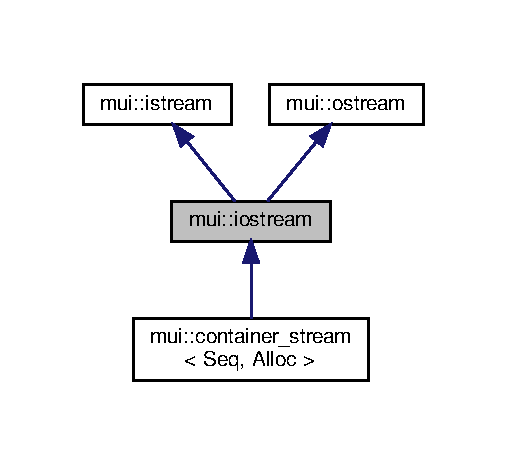
\includegraphics[width=244pt]{classmui_1_1iostream__inherit__graph}
\end{center}
\end{figure}


Collaboration diagram for mui\+:\+:iostream\+:
\nopagebreak
\begin{figure}[H]
\begin{center}
\leavevmode
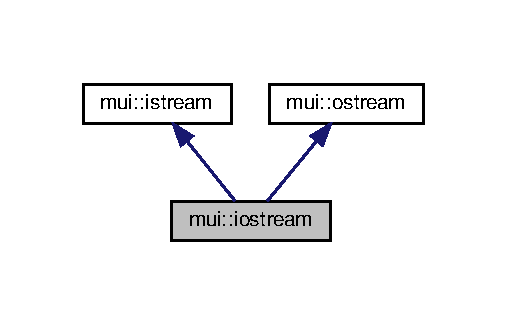
\includegraphics[width=244pt]{classmui_1_1iostream__coll__graph}
\end{center}
\end{figure}
\subsection*{Public Member Functions}
\begin{DoxyCompactItemize}
\item 
virtual \hyperlink{classmui_1_1iostream_af412ceca6334a3ad45c0ca6799ecae10}{$\sim$iostream} ()
\end{DoxyCompactItemize}


\subsection{Constructor \& Destructor Documentation}
\mbox{\Hypertarget{classmui_1_1iostream_af412ceca6334a3ad45c0ca6799ecae10}\label{classmui_1_1iostream_af412ceca6334a3ad45c0ca6799ecae10}} 
\index{mui\+::iostream@{mui\+::iostream}!````~iostream@{$\sim$iostream}}
\index{````~iostream@{$\sim$iostream}!mui\+::iostream@{mui\+::iostream}}
\subsubsection{\texorpdfstring{$\sim$iostream()}{~iostream()}}
{\footnotesize\ttfamily virtual mui\+::iostream\+::$\sim$iostream (\begin{DoxyParamCaption}{ }\end{DoxyParamCaption})\hspace{0.3cm}{\ttfamily [inline]}, {\ttfamily [virtual]}}



The documentation for this class was generated from the following file\+:\begin{DoxyCompactItemize}
\item 
\hyperlink{stream_8h}{stream.\+h}\end{DoxyCompactItemize}

\hypertarget{classmui_1_1istream}{}\section{mui\+:\+:istream Class Reference}
\label{classmui_1_1istream}\index{mui\+::istream@{mui\+::istream}}


{\ttfamily \#include $<$stream.\+h$>$}



Inheritance diagram for mui\+:\+:istream\+:
\nopagebreak
\begin{figure}[H]
\begin{center}
\leavevmode
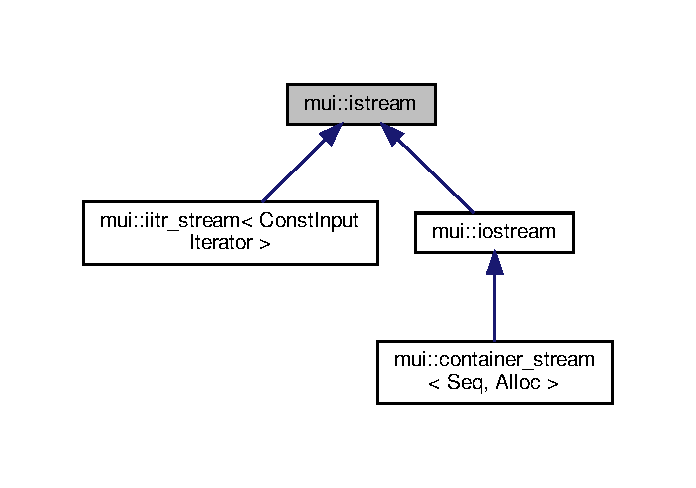
\includegraphics[width=334pt]{classmui_1_1istream__inherit__graph}
\end{center}
\end{figure}
\subsection*{Public Member Functions}
\begin{DoxyCompactItemize}
\item 
virtual \hyperlink{classmui_1_1istream_a0aaf466019e7a6f84002a738c26d2e9d}{$\sim$istream} ()
\item 
virtual void \hyperlink{classmui_1_1istream_a275ecbe530bf67df5978be288897ab45}{read} (char $\ast$ptr, std\+::size\+\_\+t size)=0
\end{DoxyCompactItemize}


\subsection{Constructor \& Destructor Documentation}
\mbox{\Hypertarget{classmui_1_1istream_a0aaf466019e7a6f84002a738c26d2e9d}\label{classmui_1_1istream_a0aaf466019e7a6f84002a738c26d2e9d}} 
\index{mui\+::istream@{mui\+::istream}!````~istream@{$\sim$istream}}
\index{````~istream@{$\sim$istream}!mui\+::istream@{mui\+::istream}}
\subsubsection{\texorpdfstring{$\sim$istream()}{~istream()}}
{\footnotesize\ttfamily virtual mui\+::istream\+::$\sim$istream (\begin{DoxyParamCaption}{ }\end{DoxyParamCaption})\hspace{0.3cm}{\ttfamily [inline]}, {\ttfamily [virtual]}}



\subsection{Member Function Documentation}
\mbox{\Hypertarget{classmui_1_1istream_a275ecbe530bf67df5978be288897ab45}\label{classmui_1_1istream_a275ecbe530bf67df5978be288897ab45}} 
\index{mui\+::istream@{mui\+::istream}!read@{read}}
\index{read@{read}!mui\+::istream@{mui\+::istream}}
\subsubsection{\texorpdfstring{read()}{read()}}
{\footnotesize\ttfamily virtual void mui\+::istream\+::read (\begin{DoxyParamCaption}\item[{char $\ast$}]{ptr,  }\item[{std\+::size\+\_\+t}]{size }\end{DoxyParamCaption})\hspace{0.3cm}{\ttfamily [pure virtual]}}



Implemented in \hyperlink{classmui_1_1iitr__stream_aa39fd880d0a4ec821775a86c0d7bc2ce}{mui\+::iitr\+\_\+stream$<$ Const\+Input\+Iterator $>$}, and \hyperlink{classmui_1_1container__stream_a6bcd220029a12f27de5443a2b48b245a}{mui\+::container\+\_\+stream$<$ Seq, Alloc $>$}.



The documentation for this class was generated from the following file\+:\begin{DoxyCompactItemize}
\item 
\hyperlink{stream_8h}{stream.\+h}\end{DoxyCompactItemize}

\hypertarget{structmui_1_1make__index__sequence}{}\section{mui\+:\+:make\+\_\+index\+\_\+sequence$<$ N $>$ Struct Template Reference}
\label{structmui_1_1make__index__sequence}\index{mui\+::make\+\_\+index\+\_\+sequence$<$ N $>$@{mui\+::make\+\_\+index\+\_\+sequence$<$ N $>$}}


{\ttfamily \#include $<$stream\+\_\+tuple.\+h$>$}

\subsection*{Public Types}
\begin{DoxyCompactItemize}
\item 
typedef \hyperlink{structmui_1_1make__index__sequence}{make\+\_\+index\+\_\+sequence}$<$ N-\/1 $>$\+::type\+::next \hyperlink{structmui_1_1make__index__sequence_a1beeb221ddf74954f1efe8c9785e1d6d}{type}
\end{DoxyCompactItemize}


\subsection{Member Typedef Documentation}
\mbox{\Hypertarget{structmui_1_1make__index__sequence_a1beeb221ddf74954f1efe8c9785e1d6d}\label{structmui_1_1make__index__sequence_a1beeb221ddf74954f1efe8c9785e1d6d}} 
\index{mui\+::make\+\_\+index\+\_\+sequence@{mui\+::make\+\_\+index\+\_\+sequence}!type@{type}}
\index{type@{type}!mui\+::make\+\_\+index\+\_\+sequence@{mui\+::make\+\_\+index\+\_\+sequence}}
\subsubsection{\texorpdfstring{type}{type}}
{\footnotesize\ttfamily template$<$std\+::size\+\_\+t N$>$ \\
typedef \hyperlink{structmui_1_1make__index__sequence}{make\+\_\+index\+\_\+sequence}$<$N-\/1$>$\+::type\+::next \hyperlink{structmui_1_1make__index__sequence}{mui\+::make\+\_\+index\+\_\+sequence}$<$ N $>$\+::\hyperlink{structmui_1_1make__index__sequence_a1beeb221ddf74954f1efe8c9785e1d6d}{type}}



The documentation for this struct was generated from the following file\+:\begin{DoxyCompactItemize}
\item 
\hyperlink{stream__tuple_8h}{stream\+\_\+tuple.\+h}\end{DoxyCompactItemize}

\hypertarget{structmui_1_1make__index__sequence_3_010_01_4}{}\section{mui\+:\+:make\+\_\+index\+\_\+sequence$<$ 0 $>$ Struct Template Reference}
\label{structmui_1_1make__index__sequence_3_010_01_4}\index{mui\+::make\+\_\+index\+\_\+sequence$<$ 0 $>$@{mui\+::make\+\_\+index\+\_\+sequence$<$ 0 $>$}}


{\ttfamily \#include $<$stream\+\_\+tuple.\+h$>$}

\subsection*{Public Types}
\begin{DoxyCompactItemize}
\item 
typedef \hyperlink{structmui_1_1index__sequence}{index\+\_\+sequence} \hyperlink{structmui_1_1make__index__sequence_3_010_01_4_a0f9c3c9185886604e73df2c025e07d40}{type}
\end{DoxyCompactItemize}


\subsection{Member Typedef Documentation}
\mbox{\Hypertarget{structmui_1_1make__index__sequence_3_010_01_4_a0f9c3c9185886604e73df2c025e07d40}\label{structmui_1_1make__index__sequence_3_010_01_4_a0f9c3c9185886604e73df2c025e07d40}} 
\index{mui\+::make\+\_\+index\+\_\+sequence$<$ 0 $>$@{mui\+::make\+\_\+index\+\_\+sequence$<$ 0 $>$}!type@{type}}
\index{type@{type}!mui\+::make\+\_\+index\+\_\+sequence$<$ 0 $>$@{mui\+::make\+\_\+index\+\_\+sequence$<$ 0 $>$}}
\subsubsection{\texorpdfstring{type}{type}}
{\footnotesize\ttfamily typedef \hyperlink{structmui_1_1index__sequence}{index\+\_\+sequence} \hyperlink{structmui_1_1make__index__sequence}{mui\+::make\+\_\+index\+\_\+sequence}$<$ 0 $>$\+::\hyperlink{structmui_1_1make__index__sequence_3_010_01_4_a0f9c3c9185886604e73df2c025e07d40}{type}}



The documentation for this struct was generated from the following file\+:\begin{DoxyCompactItemize}
\item 
\hyperlink{stream__tuple_8h}{stream\+\_\+tuple.\+h}\end{DoxyCompactItemize}

\hypertarget{structmui_1_1message}{}\section{mui\+:\+:message Struct Reference}
\label{structmui_1_1message}\index{mui\+::message@{mui\+::message}}


{\ttfamily \#include $<$message.\+h$>$}

\subsection*{Public Types}
\begin{DoxyCompactItemize}
\item 
using \hyperlink{structmui_1_1message_aecbd0ac37983ce799121a1d78d97a9c1}{id\+\_\+type} = std\+::string
\end{DoxyCompactItemize}
\subsection*{Public Member Functions}
\begin{DoxyCompactItemize}
\item 
\hyperlink{structmui_1_1message_ada5eb3ee6f884e50de90361a9dd2005a}{message} ()
\item 
bool \hyperlink{structmui_1_1message_a7c5987da00691f40c4b4b6eaf979e19e}{has\+\_\+id} () const
\item 
const \hyperlink{structmui_1_1message_aecbd0ac37983ce799121a1d78d97a9c1}{id\+\_\+type} \& \hyperlink{structmui_1_1message_a15b328d568653630c8665c1d0135cbd7}{id} () const
\item 
const char $\ast$ \hyperlink{structmui_1_1message_a8fb9fd5730cb451cc20182b736ba1bfc}{data} () const
\item 
std\+::size\+\_\+t \hyperlink{structmui_1_1message_a5cf6b0eeddeea86664e9a2f17f41a872}{size} () const
\item 
std\+::vector$<$ char $>$ \hyperlink{structmui_1_1message_a91eb72d60f7eeb165a83b9c42a898ec5}{detach} ()
\end{DoxyCompactItemize}
\subsection*{Static Public Member Functions}
\begin{DoxyCompactItemize}
\item 
{\footnotesize template$<$typename... types$>$ }\\static \hyperlink{structmui_1_1message}{message} \hyperlink{structmui_1_1message_ab75db40598b84930d88eadcefa3ae94f}{make} (const \hyperlink{structmui_1_1message_aecbd0ac37983ce799121a1d78d97a9c1}{id\+\_\+type} \&\hyperlink{structmui_1_1message_a15b328d568653630c8665c1d0135cbd7}{id}, types \&\&... \hyperlink{structmui_1_1message_a8fb9fd5730cb451cc20182b736ba1bfc}{data})
\item 
static \hyperlink{structmui_1_1message}{message} \hyperlink{structmui_1_1message_a2d47197a74abcedc0c035d5190084050}{make} (std\+::vector$<$ char $>$ \hyperlink{structmui_1_1message_a8fb9fd5730cb451cc20182b736ba1bfc}{data})
\end{DoxyCompactItemize}
\subsection*{Friends}
\begin{DoxyCompactItemize}
\item 
\hyperlink{classmui_1_1ostream}{ostream} \& \hyperlink{structmui_1_1message_a4fbfde81d9ba815d34bfb6f79a66882a}{operator$<$$<$} (\hyperlink{classmui_1_1ostream}{ostream} \&, const \hyperlink{structmui_1_1message}{message} \&)
\end{DoxyCompactItemize}


\subsection{Member Typedef Documentation}
\mbox{\Hypertarget{structmui_1_1message_aecbd0ac37983ce799121a1d78d97a9c1}\label{structmui_1_1message_aecbd0ac37983ce799121a1d78d97a9c1}} 
\index{mui\+::message@{mui\+::message}!id\+\_\+type@{id\+\_\+type}}
\index{id\+\_\+type@{id\+\_\+type}!mui\+::message@{mui\+::message}}
\subsubsection{\texorpdfstring{id\+\_\+type}{id\_type}}
{\footnotesize\ttfamily using \hyperlink{structmui_1_1message_aecbd0ac37983ce799121a1d78d97a9c1}{mui\+::message\+::id\+\_\+type} =  std\+::string}



\subsection{Constructor \& Destructor Documentation}
\mbox{\Hypertarget{structmui_1_1message_ada5eb3ee6f884e50de90361a9dd2005a}\label{structmui_1_1message_ada5eb3ee6f884e50de90361a9dd2005a}} 
\index{mui\+::message@{mui\+::message}!message@{message}}
\index{message@{message}!mui\+::message@{mui\+::message}}
\subsubsection{\texorpdfstring{message()}{message()}}
{\footnotesize\ttfamily mui\+::message\+::message (\begin{DoxyParamCaption}{ }\end{DoxyParamCaption})\hspace{0.3cm}{\ttfamily [inline]}}



\subsection{Member Function Documentation}
\mbox{\Hypertarget{structmui_1_1message_a8fb9fd5730cb451cc20182b736ba1bfc}\label{structmui_1_1message_a8fb9fd5730cb451cc20182b736ba1bfc}} 
\index{mui\+::message@{mui\+::message}!data@{data}}
\index{data@{data}!mui\+::message@{mui\+::message}}
\subsubsection{\texorpdfstring{data()}{data()}}
{\footnotesize\ttfamily const char$\ast$ mui\+::message\+::data (\begin{DoxyParamCaption}{ }\end{DoxyParamCaption}) const\hspace{0.3cm}{\ttfamily [inline]}}

\mbox{\Hypertarget{structmui_1_1message_a91eb72d60f7eeb165a83b9c42a898ec5}\label{structmui_1_1message_a91eb72d60f7eeb165a83b9c42a898ec5}} 
\index{mui\+::message@{mui\+::message}!detach@{detach}}
\index{detach@{detach}!mui\+::message@{mui\+::message}}
\subsubsection{\texorpdfstring{detach()}{detach()}}
{\footnotesize\ttfamily std\+::vector$<$char$>$ mui\+::message\+::detach (\begin{DoxyParamCaption}{ }\end{DoxyParamCaption})\hspace{0.3cm}{\ttfamily [inline]}}

\mbox{\Hypertarget{structmui_1_1message_a7c5987da00691f40c4b4b6eaf979e19e}\label{structmui_1_1message_a7c5987da00691f40c4b4b6eaf979e19e}} 
\index{mui\+::message@{mui\+::message}!has\+\_\+id@{has\+\_\+id}}
\index{has\+\_\+id@{has\+\_\+id}!mui\+::message@{mui\+::message}}
\subsubsection{\texorpdfstring{has\+\_\+id()}{has\_id()}}
{\footnotesize\ttfamily bool mui\+::message\+::has\+\_\+id (\begin{DoxyParamCaption}{ }\end{DoxyParamCaption}) const\hspace{0.3cm}{\ttfamily [inline]}}

\mbox{\Hypertarget{structmui_1_1message_a15b328d568653630c8665c1d0135cbd7}\label{structmui_1_1message_a15b328d568653630c8665c1d0135cbd7}} 
\index{mui\+::message@{mui\+::message}!id@{id}}
\index{id@{id}!mui\+::message@{mui\+::message}}
\subsubsection{\texorpdfstring{id()}{id()}}
{\footnotesize\ttfamily const \hyperlink{structmui_1_1message_aecbd0ac37983ce799121a1d78d97a9c1}{id\+\_\+type}\& mui\+::message\+::id (\begin{DoxyParamCaption}{ }\end{DoxyParamCaption}) const\hspace{0.3cm}{\ttfamily [inline]}}

\mbox{\Hypertarget{structmui_1_1message_ab75db40598b84930d88eadcefa3ae94f}\label{structmui_1_1message_ab75db40598b84930d88eadcefa3ae94f}} 
\index{mui\+::message@{mui\+::message}!make@{make}}
\index{make@{make}!mui\+::message@{mui\+::message}}
\subsubsection{\texorpdfstring{make()}{make()}\hspace{0.1cm}{\footnotesize\ttfamily [1/2]}}
{\footnotesize\ttfamily template$<$typename... types$>$ \\
static \hyperlink{structmui_1_1message}{message} mui\+::message\+::make (\begin{DoxyParamCaption}\item[{const \hyperlink{structmui_1_1message_aecbd0ac37983ce799121a1d78d97a9c1}{id\+\_\+type} \&}]{id,  }\item[{types \&\&...}]{data }\end{DoxyParamCaption})\hspace{0.3cm}{\ttfamily [inline]}, {\ttfamily [static]}}

\mbox{\Hypertarget{structmui_1_1message_a2d47197a74abcedc0c035d5190084050}\label{structmui_1_1message_a2d47197a74abcedc0c035d5190084050}} 
\index{mui\+::message@{mui\+::message}!make@{make}}
\index{make@{make}!mui\+::message@{mui\+::message}}
\subsubsection{\texorpdfstring{make()}{make()}\hspace{0.1cm}{\footnotesize\ttfamily [2/2]}}
{\footnotesize\ttfamily static \hyperlink{structmui_1_1message}{message} mui\+::message\+::make (\begin{DoxyParamCaption}\item[{std\+::vector$<$ char $>$}]{data }\end{DoxyParamCaption})\hspace{0.3cm}{\ttfamily [inline]}, {\ttfamily [static]}}

\mbox{\Hypertarget{structmui_1_1message_a5cf6b0eeddeea86664e9a2f17f41a872}\label{structmui_1_1message_a5cf6b0eeddeea86664e9a2f17f41a872}} 
\index{mui\+::message@{mui\+::message}!size@{size}}
\index{size@{size}!mui\+::message@{mui\+::message}}
\subsubsection{\texorpdfstring{size()}{size()}}
{\footnotesize\ttfamily std\+::size\+\_\+t mui\+::message\+::size (\begin{DoxyParamCaption}{ }\end{DoxyParamCaption}) const\hspace{0.3cm}{\ttfamily [inline]}}



\subsection{Friends And Related Function Documentation}
\mbox{\Hypertarget{structmui_1_1message_a4fbfde81d9ba815d34bfb6f79a66882a}\label{structmui_1_1message_a4fbfde81d9ba815d34bfb6f79a66882a}} 
\index{mui\+::message@{mui\+::message}!operator$<$$<$@{operator$<$$<$}}
\index{operator$<$$<$@{operator$<$$<$}!mui\+::message@{mui\+::message}}
\subsubsection{\texorpdfstring{operator$<$$<$}{operator<<}}
{\footnotesize\ttfamily \hyperlink{classmui_1_1ostream}{ostream}\& operator$<$$<$ (\begin{DoxyParamCaption}\item[{\hyperlink{classmui_1_1ostream}{ostream} \&}]{stream,  }\item[{const \hyperlink{structmui_1_1message}{message} \&}]{m }\end{DoxyParamCaption})\hspace{0.3cm}{\ttfamily [friend]}}



The documentation for this struct was generated from the following file\+:\begin{DoxyCompactItemize}
\item 
\hyperlink{message_8h}{message.\+h}\end{DoxyCompactItemize}

\hypertarget{classmui_1_1mpicomm__nxn}{}\section{mui\+:\+:mpicomm\+\_\+nxn Class Reference}
\label{classmui_1_1mpicomm__nxn}\index{mui\+::mpicomm\+\_\+nxn@{mui\+::mpicomm\+\_\+nxn}}


{\ttfamily \#include $<$comm\+\_\+mpi\+\_\+nxn.\+h$>$}



Inheritance diagram for mui\+:\+:mpicomm\+\_\+nxn\+:
\nopagebreak
\begin{figure}[H]
\begin{center}
\leavevmode
\includegraphics[width=182pt]{classmui_1_1mpicomm__nxn__inherit__graph}
\end{center}
\end{figure}


Collaboration diagram for mui\+:\+:mpicomm\+\_\+nxn\+:
\nopagebreak
\begin{figure}[H]
\begin{center}
\leavevmode
\includegraphics[width=182pt]{classmui_1_1mpicomm__nxn__coll__graph}
\end{center}
\end{figure}
\subsection*{Public Member Functions}
\begin{DoxyCompactItemize}
\item 
\hyperlink{classmui_1_1mpicomm__nxn_a24d70a22e6191946b0f428963f0f3d36}{mpicomm\+\_\+nxn} (int tag\+\_\+, M\+P\+I\+\_\+\+Comm local\+\_\+comm\+\_\+, M\+P\+I\+\_\+\+Comm remote\+\_\+comm)
\item 
virtual \hyperlink{classmui_1_1mpicomm__nxn_a7fe76b7f261054474e5b63e24248c1ab}{$\sim$mpicomm\+\_\+nxn} ()
\item 
virtual int \hyperlink{classmui_1_1mpicomm__nxn_aa30777638394ee6f17851f06c7793454}{local\+\_\+size} () const
\item 
virtual int \hyperlink{classmui_1_1mpicomm__nxn_ac5597865b5cad6ed82e02f40aa8333b9}{remote\+\_\+size} () const
\end{DoxyCompactItemize}
\subsection*{Protected Member Functions}
\begin{DoxyCompactItemize}
\item 
std\+::size\+\_\+t \hyperlink{classmui_1_1mpicomm__nxn_a41700dbff6ae17c428693e4d124f8a8e}{send\+\_\+impl\+\_\+} (const char $\ast$ptr, std\+::size\+\_\+t size, std\+::vector$<$ bool $>$ is\+\_\+sending)
\item 
std\+::size\+\_\+t \hyperlink{classmui_1_1mpicomm__nxn_a6536b08629d41473e0597b2d4fff794e}{recv\+\_\+impl\+\_\+} (char $\ast$ptr, std\+::size\+\_\+t size)
\item 
int \hyperlink{classmui_1_1mpicomm__nxn_afb57050d55372c84325324340e15ac42}{try\+\_\+recv\+\_\+impl\+\_\+} (char $\ast$ptr, std\+::size\+\_\+t size, std\+::size\+\_\+t $\ast$received\+\_\+size)
\end{DoxyCompactItemize}


\subsection{Constructor \& Destructor Documentation}
\mbox{\Hypertarget{classmui_1_1mpicomm__nxn_a24d70a22e6191946b0f428963f0f3d36}\label{classmui_1_1mpicomm__nxn_a24d70a22e6191946b0f428963f0f3d36}} 
\index{mui\+::mpicomm\+\_\+nxn@{mui\+::mpicomm\+\_\+nxn}!mpicomm\+\_\+nxn@{mpicomm\+\_\+nxn}}
\index{mpicomm\+\_\+nxn@{mpicomm\+\_\+nxn}!mui\+::mpicomm\+\_\+nxn@{mui\+::mpicomm\+\_\+nxn}}
\subsubsection{\texorpdfstring{mpicomm\+\_\+nxn()}{mpicomm\_nxn()}}
{\footnotesize\ttfamily mui\+::mpicomm\+\_\+nxn\+::mpicomm\+\_\+nxn (\begin{DoxyParamCaption}\item[{int}]{tag\+\_\+,  }\item[{M\+P\+I\+\_\+\+Comm}]{local\+\_\+comm\+\_\+,  }\item[{M\+P\+I\+\_\+\+Comm}]{remote\+\_\+comm }\end{DoxyParamCaption})\hspace{0.3cm}{\ttfamily [inline]}}

\mbox{\Hypertarget{classmui_1_1mpicomm__nxn_a7fe76b7f261054474e5b63e24248c1ab}\label{classmui_1_1mpicomm__nxn_a7fe76b7f261054474e5b63e24248c1ab}} 
\index{mui\+::mpicomm\+\_\+nxn@{mui\+::mpicomm\+\_\+nxn}!````~mpicomm\+\_\+nxn@{$\sim$mpicomm\+\_\+nxn}}
\index{````~mpicomm\+\_\+nxn@{$\sim$mpicomm\+\_\+nxn}!mui\+::mpicomm\+\_\+nxn@{mui\+::mpicomm\+\_\+nxn}}
\subsubsection{\texorpdfstring{$\sim$mpicomm\+\_\+nxn()}{~mpicomm\_nxn()}}
{\footnotesize\ttfamily virtual mui\+::mpicomm\+\_\+nxn\+::$\sim$mpicomm\+\_\+nxn (\begin{DoxyParamCaption}{ }\end{DoxyParamCaption})\hspace{0.3cm}{\ttfamily [inline]}, {\ttfamily [virtual]}}



\subsection{Member Function Documentation}
\mbox{\Hypertarget{classmui_1_1mpicomm__nxn_aa30777638394ee6f17851f06c7793454}\label{classmui_1_1mpicomm__nxn_aa30777638394ee6f17851f06c7793454}} 
\index{mui\+::mpicomm\+\_\+nxn@{mui\+::mpicomm\+\_\+nxn}!local\+\_\+size@{local\+\_\+size}}
\index{local\+\_\+size@{local\+\_\+size}!mui\+::mpicomm\+\_\+nxn@{mui\+::mpicomm\+\_\+nxn}}
\subsubsection{\texorpdfstring{local\+\_\+size()}{local\_size()}}
{\footnotesize\ttfamily virtual int mui\+::mpicomm\+\_\+nxn\+::local\+\_\+size (\begin{DoxyParamCaption}{ }\end{DoxyParamCaption}) const\hspace{0.3cm}{\ttfamily [inline]}, {\ttfamily [virtual]}}



Reimplemented from \hyperlink{classmui_1_1communicator_aa98faead0a9f63b8edb8b987477998e1}{mui\+::communicator}.

\mbox{\Hypertarget{classmui_1_1mpicomm__nxn_a6536b08629d41473e0597b2d4fff794e}\label{classmui_1_1mpicomm__nxn_a6536b08629d41473e0597b2d4fff794e}} 
\index{mui\+::mpicomm\+\_\+nxn@{mui\+::mpicomm\+\_\+nxn}!recv\+\_\+impl\+\_\+@{recv\+\_\+impl\+\_\+}}
\index{recv\+\_\+impl\+\_\+@{recv\+\_\+impl\+\_\+}!mui\+::mpicomm\+\_\+nxn@{mui\+::mpicomm\+\_\+nxn}}
\subsubsection{\texorpdfstring{recv\+\_\+impl\+\_\+()}{recv\_impl\_()}}
{\footnotesize\ttfamily std\+::size\+\_\+t mui\+::mpicomm\+\_\+nxn\+::recv\+\_\+impl\+\_\+ (\begin{DoxyParamCaption}\item[{char $\ast$}]{ptr,  }\item[{std\+::size\+\_\+t}]{size }\end{DoxyParamCaption})\hspace{0.3cm}{\ttfamily [inline]}, {\ttfamily [protected]}}

\mbox{\Hypertarget{classmui_1_1mpicomm__nxn_ac5597865b5cad6ed82e02f40aa8333b9}\label{classmui_1_1mpicomm__nxn_ac5597865b5cad6ed82e02f40aa8333b9}} 
\index{mui\+::mpicomm\+\_\+nxn@{mui\+::mpicomm\+\_\+nxn}!remote\+\_\+size@{remote\+\_\+size}}
\index{remote\+\_\+size@{remote\+\_\+size}!mui\+::mpicomm\+\_\+nxn@{mui\+::mpicomm\+\_\+nxn}}
\subsubsection{\texorpdfstring{remote\+\_\+size()}{remote\_size()}}
{\footnotesize\ttfamily virtual int mui\+::mpicomm\+\_\+nxn\+::remote\+\_\+size (\begin{DoxyParamCaption}{ }\end{DoxyParamCaption}) const\hspace{0.3cm}{\ttfamily [inline]}, {\ttfamily [virtual]}}



Reimplemented from \hyperlink{classmui_1_1communicator_a8683d36801b78685ce5a58da2c6a6195}{mui\+::communicator}.

\mbox{\Hypertarget{classmui_1_1mpicomm__nxn_a41700dbff6ae17c428693e4d124f8a8e}\label{classmui_1_1mpicomm__nxn_a41700dbff6ae17c428693e4d124f8a8e}} 
\index{mui\+::mpicomm\+\_\+nxn@{mui\+::mpicomm\+\_\+nxn}!send\+\_\+impl\+\_\+@{send\+\_\+impl\+\_\+}}
\index{send\+\_\+impl\+\_\+@{send\+\_\+impl\+\_\+}!mui\+::mpicomm\+\_\+nxn@{mui\+::mpicomm\+\_\+nxn}}
\subsubsection{\texorpdfstring{send\+\_\+impl\+\_\+()}{send\_impl\_()}}
{\footnotesize\ttfamily std\+::size\+\_\+t mui\+::mpicomm\+\_\+nxn\+::send\+\_\+impl\+\_\+ (\begin{DoxyParamCaption}\item[{const char $\ast$}]{ptr,  }\item[{std\+::size\+\_\+t}]{size,  }\item[{std\+::vector$<$ bool $>$}]{is\+\_\+sending }\end{DoxyParamCaption})\hspace{0.3cm}{\ttfamily [inline]}, {\ttfamily [protected]}}

\mbox{\Hypertarget{classmui_1_1mpicomm__nxn_afb57050d55372c84325324340e15ac42}\label{classmui_1_1mpicomm__nxn_afb57050d55372c84325324340e15ac42}} 
\index{mui\+::mpicomm\+\_\+nxn@{mui\+::mpicomm\+\_\+nxn}!try\+\_\+recv\+\_\+impl\+\_\+@{try\+\_\+recv\+\_\+impl\+\_\+}}
\index{try\+\_\+recv\+\_\+impl\+\_\+@{try\+\_\+recv\+\_\+impl\+\_\+}!mui\+::mpicomm\+\_\+nxn@{mui\+::mpicomm\+\_\+nxn}}
\subsubsection{\texorpdfstring{try\+\_\+recv\+\_\+impl\+\_\+()}{try\_recv\_impl\_()}}
{\footnotesize\ttfamily int mui\+::mpicomm\+\_\+nxn\+::try\+\_\+recv\+\_\+impl\+\_\+ (\begin{DoxyParamCaption}\item[{char $\ast$}]{ptr,  }\item[{std\+::size\+\_\+t}]{size,  }\item[{std\+::size\+\_\+t $\ast$}]{received\+\_\+size }\end{DoxyParamCaption})\hspace{0.3cm}{\ttfamily [inline]}, {\ttfamily [protected]}}



The documentation for this class was generated from the following file\+:\begin{DoxyCompactItemize}
\item 
\hyperlink{comm__mpi__nxn_8h}{comm\+\_\+mpi\+\_\+nxn.\+h}\end{DoxyCompactItemize}

\hypertarget{interfacemui__3df_1_1mui__create__uniface3d__f}{}\section{mui\+\_\+3df\+:\+:mui\+\_\+create\+\_\+uniface3d\+\_\+f Interface Reference}
\label{interfacemui__3df_1_1mui__create__uniface3d__f}\index{mui\+\_\+3df\+::mui\+\_\+create\+\_\+uniface3d\+\_\+f@{mui\+\_\+3df\+::mui\+\_\+create\+\_\+uniface3d\+\_\+f}}
\subsection*{Public Member Functions}
\begin{DoxyCompactItemize}
\item 
subroutine \hyperlink{interfacemui__3df_1_1mui__create__uniface3d__f_aa0c154e8d0947c39931728b21eecf7d3}{mui\+\_\+create\+\_\+uniface3d\+\_\+f} (uniface, domain)
\end{DoxyCompactItemize}


\subsection{Constructor \& Destructor Documentation}
\mbox{\Hypertarget{interfacemui__3df_1_1mui__create__uniface3d__f_aa0c154e8d0947c39931728b21eecf7d3}\label{interfacemui__3df_1_1mui__create__uniface3d__f_aa0c154e8d0947c39931728b21eecf7d3}} 
\index{mui\+\_\+3df\+::mui\+\_\+create\+\_\+uniface3d\+\_\+f@{mui\+\_\+3df\+::mui\+\_\+create\+\_\+uniface3d\+\_\+f}!mui\+\_\+create\+\_\+uniface3d\+\_\+f@{mui\+\_\+create\+\_\+uniface3d\+\_\+f}}
\index{mui\+\_\+create\+\_\+uniface3d\+\_\+f@{mui\+\_\+create\+\_\+uniface3d\+\_\+f}!mui\+\_\+3df\+::mui\+\_\+create\+\_\+uniface3d\+\_\+f@{mui\+\_\+3df\+::mui\+\_\+create\+\_\+uniface3d\+\_\+f}}
\subsubsection{\texorpdfstring{mui\+\_\+create\+\_\+uniface3d\+\_\+f()}{mui\_create\_uniface3d\_f()}}
{\footnotesize\ttfamily subroutine mui\+\_\+3df\+::mui\+\_\+create\+\_\+uniface3d\+\_\+f\+::mui\+\_\+create\+\_\+uniface3d\+\_\+f (\begin{DoxyParamCaption}\item[{type(c\+\_\+ptr), dimension($\ast$), intent(out), target}]{uniface,  }\item[{character(kind=c\+\_\+char), dimension($\ast$), intent(in)}]{domain }\end{DoxyParamCaption})}



The documentation for this interface was generated from the following file\+:\begin{DoxyCompactItemize}
\item 
wrappers/\+Fortran/\hyperlink{mui_8f90}{mui.\+f90}\end{DoxyCompactItemize}

\hypertarget{interfacemui__3df_1_1mui__destroy__uniface3d__f}{}\section{mui\+\_\+3df\+:\+:mui\+\_\+destroy\+\_\+uniface3d\+\_\+f Interface Reference}
\label{interfacemui__3df_1_1mui__destroy__uniface3d__f}\index{mui\+\_\+3df\+::mui\+\_\+destroy\+\_\+uniface3d\+\_\+f@{mui\+\_\+3df\+::mui\+\_\+destroy\+\_\+uniface3d\+\_\+f}}
\subsection*{Public Member Functions}
\begin{DoxyCompactItemize}
\item 
subroutine \hyperlink{interfacemui__3df_1_1mui__destroy__uniface3d__f_acf184eb90801b6a68c3e15c2bfd46946}{mui\+\_\+destroy\+\_\+uniface3d\+\_\+f} (uniface)
\end{DoxyCompactItemize}


\subsection{Constructor \& Destructor Documentation}
\mbox{\Hypertarget{interfacemui__3df_1_1mui__destroy__uniface3d__f_acf184eb90801b6a68c3e15c2bfd46946}\label{interfacemui__3df_1_1mui__destroy__uniface3d__f_acf184eb90801b6a68c3e15c2bfd46946}} 
\index{mui\+\_\+3df\+::mui\+\_\+destroy\+\_\+uniface3d\+\_\+f@{mui\+\_\+3df\+::mui\+\_\+destroy\+\_\+uniface3d\+\_\+f}!mui\+\_\+destroy\+\_\+uniface3d\+\_\+f@{mui\+\_\+destroy\+\_\+uniface3d\+\_\+f}}
\index{mui\+\_\+destroy\+\_\+uniface3d\+\_\+f@{mui\+\_\+destroy\+\_\+uniface3d\+\_\+f}!mui\+\_\+3df\+::mui\+\_\+destroy\+\_\+uniface3d\+\_\+f@{mui\+\_\+3df\+::mui\+\_\+destroy\+\_\+uniface3d\+\_\+f}}
\subsubsection{\texorpdfstring{mui\+\_\+destroy\+\_\+uniface3d\+\_\+f()}{mui\_destroy\_uniface3d\_f()}}
{\footnotesize\ttfamily subroutine mui\+\_\+3df\+::mui\+\_\+destroy\+\_\+uniface3d\+\_\+f\+::mui\+\_\+destroy\+\_\+uniface3d\+\_\+f (\begin{DoxyParamCaption}\item[{type(c\+\_\+ptr), intent(in), value}]{uniface }\end{DoxyParamCaption})}



The documentation for this interface was generated from the following file\+:\begin{DoxyCompactItemize}
\item 
wrappers/\+Fortran/\hyperlink{mui_8f90}{mui.\+f90}\end{DoxyCompactItemize}

\hypertarget{interfacemui__3df_1_1mui__push__f}{}\section{mui\+\_\+3df\+:\+:mui\+\_\+push\+\_\+f Interface Reference}
\label{interfacemui__3df_1_1mui__push__f}\index{mui\+\_\+3df\+::mui\+\_\+push\+\_\+f@{mui\+\_\+3df\+::mui\+\_\+push\+\_\+f}}
\subsection*{Public Member Functions}
\begin{DoxyCompactItemize}
\item 
subroutine \hyperlink{interfacemui__3df_1_1mui__push__f_a20baa87cdf690fad8cdeff26b44bc177}{mui\+\_\+push\+\_\+f} (uniface, attr, x, y, z, val)
\end{DoxyCompactItemize}


\subsection{Constructor \& Destructor Documentation}
\mbox{\Hypertarget{interfacemui__3df_1_1mui__push__f_a20baa87cdf690fad8cdeff26b44bc177}\label{interfacemui__3df_1_1mui__push__f_a20baa87cdf690fad8cdeff26b44bc177}} 
\index{mui\+\_\+3df\+::mui\+\_\+push\+\_\+f@{mui\+\_\+3df\+::mui\+\_\+push\+\_\+f}!mui\+\_\+push\+\_\+f@{mui\+\_\+push\+\_\+f}}
\index{mui\+\_\+push\+\_\+f@{mui\+\_\+push\+\_\+f}!mui\+\_\+3df\+::mui\+\_\+push\+\_\+f@{mui\+\_\+3df\+::mui\+\_\+push\+\_\+f}}
\subsubsection{\texorpdfstring{mui\+\_\+push\+\_\+f()}{mui\_push\_f()}}
{\footnotesize\ttfamily subroutine mui\+\_\+3df\+::mui\+\_\+push\+\_\+f\+::mui\+\_\+push\+\_\+f (\begin{DoxyParamCaption}\item[{type(c\+\_\+ptr), intent(in), value}]{uniface,  }\item[{character(kind=c\+\_\+char), dimension($\ast$), intent(in)}]{attr,  }\item[{real(kind=c\+\_\+double), intent(in)}]{x,  }\item[{real(kind=c\+\_\+double), intent(in)}]{y,  }\item[{real(kind=c\+\_\+double), intent(in)}]{z,  }\item[{real(kind=c\+\_\+double), intent(in)}]{val }\end{DoxyParamCaption})}



The documentation for this interface was generated from the following file\+:\begin{DoxyCompactItemize}
\item 
wrappers/\+Fortran/\hyperlink{mui_8f90}{mui.\+f90}\end{DoxyCompactItemize}

\hypertarget{structmui_1_1mutex__timeout}{}\section{mui\+:\+:mutex\+\_\+timeout Struct Reference}
\label{structmui_1_1mutex__timeout}\index{mui\+::mutex\+\_\+timeout@{mui\+::mutex\+\_\+timeout}}


{\ttfamily \#include $<$comm\+\_\+tcp.\+h$>$}



Inheritance diagram for mui\+:\+:mutex\+\_\+timeout\+:
\nopagebreak
\begin{figure}[H]
\begin{center}
\leavevmode
\includegraphics[width=183pt]{structmui_1_1mutex__timeout__inherit__graph}
\end{center}
\end{figure}


Collaboration diagram for mui\+:\+:mutex\+\_\+timeout\+:
\nopagebreak
\begin{figure}[H]
\begin{center}
\leavevmode
\includegraphics[width=183pt]{structmui_1_1mutex__timeout__coll__graph}
\end{center}
\end{figure}
\subsection*{Public Member Functions}
\begin{DoxyCompactItemize}
\item 
\hyperlink{structmui_1_1mutex__timeout_adb40b0f731b2d2b87fed031e10356f38}{mutex\+\_\+timeout} ()
\end{DoxyCompactItemize}


\subsection{Constructor \& Destructor Documentation}
\mbox{\Hypertarget{structmui_1_1mutex__timeout_adb40b0f731b2d2b87fed031e10356f38}\label{structmui_1_1mutex__timeout_adb40b0f731b2d2b87fed031e10356f38}} 
\index{mui\+::mutex\+\_\+timeout@{mui\+::mutex\+\_\+timeout}!mutex\+\_\+timeout@{mutex\+\_\+timeout}}
\index{mutex\+\_\+timeout@{mutex\+\_\+timeout}!mui\+::mutex\+\_\+timeout@{mui\+::mutex\+\_\+timeout}}
\subsubsection{\texorpdfstring{mutex\+\_\+timeout()}{mutex\_timeout()}}
{\footnotesize\ttfamily mui\+::mutex\+\_\+timeout\+::mutex\+\_\+timeout (\begin{DoxyParamCaption}{ }\end{DoxyParamCaption})\hspace{0.3cm}{\ttfamily [inline]}}



The documentation for this struct was generated from the following file\+:\begin{DoxyCompactItemize}
\item 
\hyperlink{comm__tcp_8h}{comm\+\_\+tcp.\+h}\end{DoxyCompactItemize}

\hypertarget{classmui_1_1ocount__stream}{}\section{mui\+:\+:ocount\+\_\+stream Class Reference}
\label{classmui_1_1ocount__stream}\index{mui\+::ocount\+\_\+stream@{mui\+::ocount\+\_\+stream}}


{\ttfamily \#include $<$stream.\+h$>$}



Inheritance diagram for mui\+:\+:ocount\+\_\+stream\+:
\nopagebreak
\begin{figure}[H]
\begin{center}
\leavevmode
\includegraphics[width=183pt]{classmui_1_1ocount__stream__inherit__graph}
\end{center}
\end{figure}


Collaboration diagram for mui\+:\+:ocount\+\_\+stream\+:
\nopagebreak
\begin{figure}[H]
\begin{center}
\leavevmode
\includegraphics[width=183pt]{classmui_1_1ocount__stream__coll__graph}
\end{center}
\end{figure}
\subsection*{Public Member Functions}
\begin{DoxyCompactItemize}
\item 
\hyperlink{classmui_1_1ocount__stream_ab156198b5e8f4abddbcd284ad30f2a17}{ocount\+\_\+stream} (std\+::size\+\_\+t off=0u)
\item 
\hyperlink{classmui_1_1ocount__stream_a036bf20fdc27902a7a4770f576a90f77}{$\sim$ocount\+\_\+stream} ()
\item 
std\+::size\+\_\+t \hyperlink{classmui_1_1ocount__stream_a02a11f05e4411c05516e4bc2ec705128}{size} () const
\item 
void \hyperlink{classmui_1_1ocount__stream_a7d536099a215a5546eef065634b7ea67}{write} (const char $\ast$, std\+::size\+\_\+t \hyperlink{classmui_1_1ocount__stream_a02a11f05e4411c05516e4bc2ec705128}{size})
\end{DoxyCompactItemize}


\subsection{Constructor \& Destructor Documentation}
\mbox{\Hypertarget{classmui_1_1ocount__stream_ab156198b5e8f4abddbcd284ad30f2a17}\label{classmui_1_1ocount__stream_ab156198b5e8f4abddbcd284ad30f2a17}} 
\index{mui\+::ocount\+\_\+stream@{mui\+::ocount\+\_\+stream}!ocount\+\_\+stream@{ocount\+\_\+stream}}
\index{ocount\+\_\+stream@{ocount\+\_\+stream}!mui\+::ocount\+\_\+stream@{mui\+::ocount\+\_\+stream}}
\subsubsection{\texorpdfstring{ocount\+\_\+stream()}{ocount\_stream()}}
{\footnotesize\ttfamily mui\+::ocount\+\_\+stream\+::ocount\+\_\+stream (\begin{DoxyParamCaption}\item[{std\+::size\+\_\+t}]{off = {\ttfamily 0u} }\end{DoxyParamCaption})\hspace{0.3cm}{\ttfamily [inline]}}

\mbox{\Hypertarget{classmui_1_1ocount__stream_a036bf20fdc27902a7a4770f576a90f77}\label{classmui_1_1ocount__stream_a036bf20fdc27902a7a4770f576a90f77}} 
\index{mui\+::ocount\+\_\+stream@{mui\+::ocount\+\_\+stream}!````~ocount\+\_\+stream@{$\sim$ocount\+\_\+stream}}
\index{````~ocount\+\_\+stream@{$\sim$ocount\+\_\+stream}!mui\+::ocount\+\_\+stream@{mui\+::ocount\+\_\+stream}}
\subsubsection{\texorpdfstring{$\sim$ocount\+\_\+stream()}{~ocount\_stream()}}
{\footnotesize\ttfamily mui\+::ocount\+\_\+stream\+::$\sim$ocount\+\_\+stream (\begin{DoxyParamCaption}{ }\end{DoxyParamCaption})\hspace{0.3cm}{\ttfamily [inline]}}



\subsection{Member Function Documentation}
\mbox{\Hypertarget{classmui_1_1ocount__stream_a02a11f05e4411c05516e4bc2ec705128}\label{classmui_1_1ocount__stream_a02a11f05e4411c05516e4bc2ec705128}} 
\index{mui\+::ocount\+\_\+stream@{mui\+::ocount\+\_\+stream}!size@{size}}
\index{size@{size}!mui\+::ocount\+\_\+stream@{mui\+::ocount\+\_\+stream}}
\subsubsection{\texorpdfstring{size()}{size()}}
{\footnotesize\ttfamily std\+::size\+\_\+t mui\+::ocount\+\_\+stream\+::size (\begin{DoxyParamCaption}{ }\end{DoxyParamCaption}) const\hspace{0.3cm}{\ttfamily [inline]}}

\mbox{\Hypertarget{classmui_1_1ocount__stream_a7d536099a215a5546eef065634b7ea67}\label{classmui_1_1ocount__stream_a7d536099a215a5546eef065634b7ea67}} 
\index{mui\+::ocount\+\_\+stream@{mui\+::ocount\+\_\+stream}!write@{write}}
\index{write@{write}!mui\+::ocount\+\_\+stream@{mui\+::ocount\+\_\+stream}}
\subsubsection{\texorpdfstring{write()}{write()}}
{\footnotesize\ttfamily void mui\+::ocount\+\_\+stream\+::write (\begin{DoxyParamCaption}\item[{const char $\ast$}]{,  }\item[{std\+::size\+\_\+t}]{size }\end{DoxyParamCaption})\hspace{0.3cm}{\ttfamily [inline]}, {\ttfamily [virtual]}}



Implements \hyperlink{classmui_1_1ostream_a93a0a1d32007efc375d885181c833995}{mui\+::ostream}.



The documentation for this class was generated from the following file\+:\begin{DoxyCompactItemize}
\item 
\hyperlink{stream_8h}{stream.\+h}\end{DoxyCompactItemize}

\hypertarget{classmui_1_1oitr__stream}{}\section{mui\+:\+:oitr\+\_\+stream$<$ Output\+Iterator $>$ Class Template Reference}
\label{classmui_1_1oitr__stream}\index{mui\+::oitr\+\_\+stream$<$ Output\+Iterator $>$@{mui\+::oitr\+\_\+stream$<$ Output\+Iterator $>$}}


{\ttfamily \#include $<$stream.\+h$>$}



Inheritance diagram for mui\+:\+:oitr\+\_\+stream$<$ Output\+Iterator $>$\+:
\nopagebreak
\begin{figure}[H]
\begin{center}
\leavevmode
\includegraphics[width=205pt]{classmui_1_1oitr__stream__inherit__graph}
\end{center}
\end{figure}


Collaboration diagram for mui\+:\+:oitr\+\_\+stream$<$ Output\+Iterator $>$\+:
\nopagebreak
\begin{figure}[H]
\begin{center}
\leavevmode
\includegraphics[width=205pt]{classmui_1_1oitr__stream__coll__graph}
\end{center}
\end{figure}
\subsection*{Public Member Functions}
\begin{DoxyCompactItemize}
\item 
\hyperlink{classmui_1_1oitr__stream_afde8e626cc976904af23c91fd74872cc}{oitr\+\_\+stream} (const \hyperlink{classmui_1_1oitr__stream}{oitr\+\_\+stream} \&)=default
\item 
\hyperlink{classmui_1_1oitr__stream_aadb5539d92ab1188615cda0d187feae9}{oitr\+\_\+stream} (Output\+Iterator begin)
\item 
\hyperlink{classmui_1_1oitr__stream_a5d50d06cd1c0a473c614eaa32648fba4}{$\sim$oitr\+\_\+stream} ()
\item 
void \hyperlink{classmui_1_1oitr__stream_aa726d0d57ba12ede019d019d382eb4cf}{write} (const char $\ast$ptr, std\+::size\+\_\+t sz)
\item 
Output\+Iterator \hyperlink{classmui_1_1oitr__stream_a8ee33091cd47f94182e3843a5d5d2649}{current} () const
\end{DoxyCompactItemize}


\subsection{Constructor \& Destructor Documentation}
\mbox{\Hypertarget{classmui_1_1oitr__stream_afde8e626cc976904af23c91fd74872cc}\label{classmui_1_1oitr__stream_afde8e626cc976904af23c91fd74872cc}} 
\index{mui\+::oitr\+\_\+stream@{mui\+::oitr\+\_\+stream}!oitr\+\_\+stream@{oitr\+\_\+stream}}
\index{oitr\+\_\+stream@{oitr\+\_\+stream}!mui\+::oitr\+\_\+stream@{mui\+::oitr\+\_\+stream}}
\subsubsection{\texorpdfstring{oitr\+\_\+stream()}{oitr\_stream()}\hspace{0.1cm}{\footnotesize\ttfamily [1/2]}}
{\footnotesize\ttfamily template$<$typename Output\+Iterator $>$ \\
\hyperlink{classmui_1_1oitr__stream}{mui\+::oitr\+\_\+stream}$<$ Output\+Iterator $>$\+::\hyperlink{classmui_1_1oitr__stream}{oitr\+\_\+stream} (\begin{DoxyParamCaption}\item[{const \hyperlink{classmui_1_1oitr__stream}{oitr\+\_\+stream}$<$ Output\+Iterator $>$ \&}]{ }\end{DoxyParamCaption})\hspace{0.3cm}{\ttfamily [default]}}

\mbox{\Hypertarget{classmui_1_1oitr__stream_aadb5539d92ab1188615cda0d187feae9}\label{classmui_1_1oitr__stream_aadb5539d92ab1188615cda0d187feae9}} 
\index{mui\+::oitr\+\_\+stream@{mui\+::oitr\+\_\+stream}!oitr\+\_\+stream@{oitr\+\_\+stream}}
\index{oitr\+\_\+stream@{oitr\+\_\+stream}!mui\+::oitr\+\_\+stream@{mui\+::oitr\+\_\+stream}}
\subsubsection{\texorpdfstring{oitr\+\_\+stream()}{oitr\_stream()}\hspace{0.1cm}{\footnotesize\ttfamily [2/2]}}
{\footnotesize\ttfamily template$<$typename Output\+Iterator $>$ \\
\hyperlink{classmui_1_1oitr__stream}{mui\+::oitr\+\_\+stream}$<$ Output\+Iterator $>$\+::\hyperlink{classmui_1_1oitr__stream}{oitr\+\_\+stream} (\begin{DoxyParamCaption}\item[{Output\+Iterator}]{begin }\end{DoxyParamCaption})\hspace{0.3cm}{\ttfamily [inline]}}

\mbox{\Hypertarget{classmui_1_1oitr__stream_a5d50d06cd1c0a473c614eaa32648fba4}\label{classmui_1_1oitr__stream_a5d50d06cd1c0a473c614eaa32648fba4}} 
\index{mui\+::oitr\+\_\+stream@{mui\+::oitr\+\_\+stream}!````~oitr\+\_\+stream@{$\sim$oitr\+\_\+stream}}
\index{````~oitr\+\_\+stream@{$\sim$oitr\+\_\+stream}!mui\+::oitr\+\_\+stream@{mui\+::oitr\+\_\+stream}}
\subsubsection{\texorpdfstring{$\sim$oitr\+\_\+stream()}{~oitr\_stream()}}
{\footnotesize\ttfamily template$<$typename Output\+Iterator $>$ \\
\hyperlink{classmui_1_1oitr__stream}{mui\+::oitr\+\_\+stream}$<$ Output\+Iterator $>$\+::$\sim$\hyperlink{classmui_1_1oitr__stream}{oitr\+\_\+stream} (\begin{DoxyParamCaption}{ }\end{DoxyParamCaption})\hspace{0.3cm}{\ttfamily [inline]}}



\subsection{Member Function Documentation}
\mbox{\Hypertarget{classmui_1_1oitr__stream_a8ee33091cd47f94182e3843a5d5d2649}\label{classmui_1_1oitr__stream_a8ee33091cd47f94182e3843a5d5d2649}} 
\index{mui\+::oitr\+\_\+stream@{mui\+::oitr\+\_\+stream}!current@{current}}
\index{current@{current}!mui\+::oitr\+\_\+stream@{mui\+::oitr\+\_\+stream}}
\subsubsection{\texorpdfstring{current()}{current()}}
{\footnotesize\ttfamily template$<$typename Output\+Iterator $>$ \\
Output\+Iterator \hyperlink{classmui_1_1oitr__stream}{mui\+::oitr\+\_\+stream}$<$ Output\+Iterator $>$\+::current (\begin{DoxyParamCaption}{ }\end{DoxyParamCaption}) const\hspace{0.3cm}{\ttfamily [inline]}}

\mbox{\Hypertarget{classmui_1_1oitr__stream_aa726d0d57ba12ede019d019d382eb4cf}\label{classmui_1_1oitr__stream_aa726d0d57ba12ede019d019d382eb4cf}} 
\index{mui\+::oitr\+\_\+stream@{mui\+::oitr\+\_\+stream}!write@{write}}
\index{write@{write}!mui\+::oitr\+\_\+stream@{mui\+::oitr\+\_\+stream}}
\subsubsection{\texorpdfstring{write()}{write()}}
{\footnotesize\ttfamily template$<$typename Output\+Iterator $>$ \\
void \hyperlink{classmui_1_1oitr__stream}{mui\+::oitr\+\_\+stream}$<$ Output\+Iterator $>$\+::write (\begin{DoxyParamCaption}\item[{const char $\ast$}]{ptr,  }\item[{std\+::size\+\_\+t}]{sz }\end{DoxyParamCaption})\hspace{0.3cm}{\ttfamily [inline]}, {\ttfamily [virtual]}}



Implements \hyperlink{classmui_1_1ostream_a93a0a1d32007efc375d885181c833995}{mui\+::ostream}.



The documentation for this class was generated from the following file\+:\begin{DoxyCompactItemize}
\item 
\hyperlink{stream_8h}{stream.\+h}\end{DoxyCompactItemize}

\hypertarget{classmui_1_1geometry_1_1or__set}{}\section{mui\+:\+:geometry\+:\+:or\+\_\+set$<$ C\+O\+N\+F\+IG $>$ Class Template Reference}
\label{classmui_1_1geometry_1_1or__set}\index{mui\+::geometry\+::or\+\_\+set$<$ C\+O\+N\+F\+I\+G $>$@{mui\+::geometry\+::or\+\_\+set$<$ C\+O\+N\+F\+I\+G $>$}}


{\ttfamily \#include $<$geometry.\+h$>$}



Inheritance diagram for mui\+:\+:geometry\+:\+:or\+\_\+set$<$ C\+O\+N\+F\+IG $>$\+:
\nopagebreak
\begin{figure}[H]
\begin{center}
\leavevmode
\includegraphics[width=192pt]{classmui_1_1geometry_1_1or__set__inherit__graph}
\end{center}
\end{figure}


Collaboration diagram for mui\+:\+:geometry\+:\+:or\+\_\+set$<$ C\+O\+N\+F\+IG $>$\+:
\nopagebreak
\begin{figure}[H]
\begin{center}
\leavevmode
\includegraphics[width=192pt]{classmui_1_1geometry_1_1or__set__coll__graph}
\end{center}
\end{figure}
\subsection*{Public Member Functions}
\begin{DoxyCompactItemize}
\item 
\hyperlink{classmui_1_1geometry_1_1or__set_abe2bca43b4f0f8ab5f303110e0e3cee9}{or\+\_\+set} ()=default
\item 
\hyperlink{classmui_1_1geometry_1_1or__set_af7cc1f5c494421966a751692afc3e4dc}{or\+\_\+set} (\hyperlink{classmui_1_1geometry_1_1any__shape}{any\+\_\+shape}$<$ C\+O\+N\+F\+IG $>$ obj1, \hyperlink{classmui_1_1geometry_1_1any__shape}{any\+\_\+shape}$<$ C\+O\+N\+F\+IG $>$ \&obj2)
\item 
const \hyperlink{classmui_1_1geometry_1_1any__shape}{any\+\_\+shape}$<$ C\+O\+N\+F\+IG $>$ \& \hyperlink{classmui_1_1geometry_1_1or__set_a143434f556a636e3c8ea7bc71cca5286}{left} () const
\item 
\hyperlink{classmui_1_1geometry_1_1any__shape}{any\+\_\+shape}$<$ C\+O\+N\+F\+IG $>$ \& \hyperlink{classmui_1_1geometry_1_1or__set_a7bd5c9d4fbf04d0ad98ea2422cb94bfe}{left} ()
\item 
const \hyperlink{classmui_1_1geometry_1_1any__shape}{any\+\_\+shape}$<$ C\+O\+N\+F\+IG $>$ \& \hyperlink{classmui_1_1geometry_1_1or__set_acb22c551a32b377ae7169d311a29eaa8}{right} () const
\item 
\hyperlink{classmui_1_1geometry_1_1any__shape}{any\+\_\+shape}$<$ C\+O\+N\+F\+IG $>$ \& \hyperlink{classmui_1_1geometry_1_1or__set_a6eb0ff8df7bb78b4234afca52f68889b}{right} ()
\item 
\hyperlink{classmui_1_1geometry_1_1shape}{shape}$<$ C\+O\+N\+F\+IG $>$ $\ast$ \hyperlink{classmui_1_1geometry_1_1or__set_a265ef0385d0822f3222e0ef669eb4fc5}{clone} () const
\item 
\hyperlink{namespacemui_1_1geometry_a5f311a343181e2f20482e5c9afb0f136}{shape\+\_\+type} \hyperlink{classmui_1_1geometry_1_1or__set_a1cb6c72bb7be1fca6ccd038cf6d6946e}{type} () const noexcept
\item 
\hyperlink{classmui_1_1geometry_1_1box}{box}$<$ C\+O\+N\+F\+IG $>$ \hyperlink{classmui_1_1geometry_1_1or__set_ac5789620d2af6810d8f7c02d5190429f}{bbox} () const
\item 
void \hyperlink{classmui_1_1geometry_1_1or__set_ae761a2812fb9749e7df978a50b72cd76}{serialize} (\hyperlink{classmui_1_1ostream}{ostream} \&stream) const
\item 
void \hyperlink{classmui_1_1geometry_1_1or__set_ad08aaf634078ee8407ab86de77576391}{deserialize} (\hyperlink{classmui_1_1istream}{istream} \&stream)
\end{DoxyCompactItemize}
\subsection*{Additional Inherited Members}


\subsection{Constructor \& Destructor Documentation}
\mbox{\Hypertarget{classmui_1_1geometry_1_1or__set_abe2bca43b4f0f8ab5f303110e0e3cee9}\label{classmui_1_1geometry_1_1or__set_abe2bca43b4f0f8ab5f303110e0e3cee9}} 
\index{mui\+::geometry\+::or\+\_\+set@{mui\+::geometry\+::or\+\_\+set}!or\+\_\+set@{or\+\_\+set}}
\index{or\+\_\+set@{or\+\_\+set}!mui\+::geometry\+::or\+\_\+set@{mui\+::geometry\+::or\+\_\+set}}
\subsubsection{\texorpdfstring{or\+\_\+set()}{or\_set()}\hspace{0.1cm}{\footnotesize\ttfamily [1/2]}}
{\footnotesize\ttfamily template$<$typename C\+O\+N\+F\+IG $>$ \\
\hyperlink{classmui_1_1geometry_1_1or__set}{mui\+::geometry\+::or\+\_\+set}$<$ C\+O\+N\+F\+IG $>$\+::\hyperlink{classmui_1_1geometry_1_1or__set}{or\+\_\+set} (\begin{DoxyParamCaption}{ }\end{DoxyParamCaption})\hspace{0.3cm}{\ttfamily [default]}}

\mbox{\Hypertarget{classmui_1_1geometry_1_1or__set_af7cc1f5c494421966a751692afc3e4dc}\label{classmui_1_1geometry_1_1or__set_af7cc1f5c494421966a751692afc3e4dc}} 
\index{mui\+::geometry\+::or\+\_\+set@{mui\+::geometry\+::or\+\_\+set}!or\+\_\+set@{or\+\_\+set}}
\index{or\+\_\+set@{or\+\_\+set}!mui\+::geometry\+::or\+\_\+set@{mui\+::geometry\+::or\+\_\+set}}
\subsubsection{\texorpdfstring{or\+\_\+set()}{or\_set()}\hspace{0.1cm}{\footnotesize\ttfamily [2/2]}}
{\footnotesize\ttfamily template$<$typename C\+O\+N\+F\+IG $>$ \\
\hyperlink{classmui_1_1geometry_1_1or__set}{mui\+::geometry\+::or\+\_\+set}$<$ C\+O\+N\+F\+IG $>$\+::\hyperlink{classmui_1_1geometry_1_1or__set}{or\+\_\+set} (\begin{DoxyParamCaption}\item[{\hyperlink{classmui_1_1geometry_1_1any__shape}{any\+\_\+shape}$<$ C\+O\+N\+F\+IG $>$}]{obj1,  }\item[{\hyperlink{classmui_1_1geometry_1_1any__shape}{any\+\_\+shape}$<$ C\+O\+N\+F\+IG $>$ \&}]{obj2 }\end{DoxyParamCaption})\hspace{0.3cm}{\ttfamily [inline]}}



\subsection{Member Function Documentation}
\mbox{\Hypertarget{classmui_1_1geometry_1_1or__set_ac5789620d2af6810d8f7c02d5190429f}\label{classmui_1_1geometry_1_1or__set_ac5789620d2af6810d8f7c02d5190429f}} 
\index{mui\+::geometry\+::or\+\_\+set@{mui\+::geometry\+::or\+\_\+set}!bbox@{bbox}}
\index{bbox@{bbox}!mui\+::geometry\+::or\+\_\+set@{mui\+::geometry\+::or\+\_\+set}}
\subsubsection{\texorpdfstring{bbox()}{bbox()}}
{\footnotesize\ttfamily template$<$typename C\+O\+N\+F\+IG $>$ \\
\hyperlink{classmui_1_1geometry_1_1box}{box}$<$ C\+O\+N\+F\+IG $>$ \hyperlink{classmui_1_1geometry_1_1or__set}{mui\+::geometry\+::or\+\_\+set}$<$ C\+O\+N\+F\+IG $>$\+::bbox (\begin{DoxyParamCaption}{ }\end{DoxyParamCaption}) const\hspace{0.3cm}{\ttfamily [virtual]}}



Implements \hyperlink{classmui_1_1geometry_1_1shape_adf598ec651ea425553bd8e617cac7430}{mui\+::geometry\+::shape$<$ C\+O\+N\+F\+I\+G $>$}.

\mbox{\Hypertarget{classmui_1_1geometry_1_1or__set_a265ef0385d0822f3222e0ef669eb4fc5}\label{classmui_1_1geometry_1_1or__set_a265ef0385d0822f3222e0ef669eb4fc5}} 
\index{mui\+::geometry\+::or\+\_\+set@{mui\+::geometry\+::or\+\_\+set}!clone@{clone}}
\index{clone@{clone}!mui\+::geometry\+::or\+\_\+set@{mui\+::geometry\+::or\+\_\+set}}
\subsubsection{\texorpdfstring{clone()}{clone()}}
{\footnotesize\ttfamily template$<$typename C\+O\+N\+F\+IG $>$ \\
\hyperlink{classmui_1_1geometry_1_1shape}{shape}$<$C\+O\+N\+F\+IG$>$$\ast$ \hyperlink{classmui_1_1geometry_1_1or__set}{mui\+::geometry\+::or\+\_\+set}$<$ C\+O\+N\+F\+IG $>$\+::clone (\begin{DoxyParamCaption}{ }\end{DoxyParamCaption}) const\hspace{0.3cm}{\ttfamily [inline]}, {\ttfamily [virtual]}}



Implements \hyperlink{classmui_1_1geometry_1_1shape_a4d1307ebc40d462b13da89c811b3beb7}{mui\+::geometry\+::shape$<$ C\+O\+N\+F\+I\+G $>$}.

\mbox{\Hypertarget{classmui_1_1geometry_1_1or__set_ad08aaf634078ee8407ab86de77576391}\label{classmui_1_1geometry_1_1or__set_ad08aaf634078ee8407ab86de77576391}} 
\index{mui\+::geometry\+::or\+\_\+set@{mui\+::geometry\+::or\+\_\+set}!deserialize@{deserialize}}
\index{deserialize@{deserialize}!mui\+::geometry\+::or\+\_\+set@{mui\+::geometry\+::or\+\_\+set}}
\subsubsection{\texorpdfstring{deserialize()}{deserialize()}}
{\footnotesize\ttfamily template$<$typename C\+O\+N\+F\+IG $>$ \\
void \hyperlink{classmui_1_1geometry_1_1or__set}{mui\+::geometry\+::or\+\_\+set}$<$ C\+O\+N\+F\+IG $>$\+::deserialize (\begin{DoxyParamCaption}\item[{\hyperlink{classmui_1_1istream}{istream} \&}]{stream }\end{DoxyParamCaption})\hspace{0.3cm}{\ttfamily [inline]}, {\ttfamily [virtual]}}



Implements \hyperlink{classmui_1_1geometry_1_1shape_ae68c7e1a1ae362abec52edad5489a1a9}{mui\+::geometry\+::shape$<$ C\+O\+N\+F\+I\+G $>$}.

\mbox{\Hypertarget{classmui_1_1geometry_1_1or__set_a143434f556a636e3c8ea7bc71cca5286}\label{classmui_1_1geometry_1_1or__set_a143434f556a636e3c8ea7bc71cca5286}} 
\index{mui\+::geometry\+::or\+\_\+set@{mui\+::geometry\+::or\+\_\+set}!left@{left}}
\index{left@{left}!mui\+::geometry\+::or\+\_\+set@{mui\+::geometry\+::or\+\_\+set}}
\subsubsection{\texorpdfstring{left()}{left()}\hspace{0.1cm}{\footnotesize\ttfamily [1/2]}}
{\footnotesize\ttfamily template$<$typename C\+O\+N\+F\+IG $>$ \\
const \hyperlink{classmui_1_1geometry_1_1any__shape}{any\+\_\+shape}$<$C\+O\+N\+F\+IG$>$\& \hyperlink{classmui_1_1geometry_1_1or__set}{mui\+::geometry\+::or\+\_\+set}$<$ C\+O\+N\+F\+IG $>$\+::left (\begin{DoxyParamCaption}{ }\end{DoxyParamCaption}) const\hspace{0.3cm}{\ttfamily [inline]}}

\mbox{\Hypertarget{classmui_1_1geometry_1_1or__set_a7bd5c9d4fbf04d0ad98ea2422cb94bfe}\label{classmui_1_1geometry_1_1or__set_a7bd5c9d4fbf04d0ad98ea2422cb94bfe}} 
\index{mui\+::geometry\+::or\+\_\+set@{mui\+::geometry\+::or\+\_\+set}!left@{left}}
\index{left@{left}!mui\+::geometry\+::or\+\_\+set@{mui\+::geometry\+::or\+\_\+set}}
\subsubsection{\texorpdfstring{left()}{left()}\hspace{0.1cm}{\footnotesize\ttfamily [2/2]}}
{\footnotesize\ttfamily template$<$typename C\+O\+N\+F\+IG $>$ \\
\hyperlink{classmui_1_1geometry_1_1any__shape}{any\+\_\+shape}$<$C\+O\+N\+F\+IG$>$\& \hyperlink{classmui_1_1geometry_1_1or__set}{mui\+::geometry\+::or\+\_\+set}$<$ C\+O\+N\+F\+IG $>$\+::left (\begin{DoxyParamCaption}{ }\end{DoxyParamCaption})\hspace{0.3cm}{\ttfamily [inline]}}

\mbox{\Hypertarget{classmui_1_1geometry_1_1or__set_acb22c551a32b377ae7169d311a29eaa8}\label{classmui_1_1geometry_1_1or__set_acb22c551a32b377ae7169d311a29eaa8}} 
\index{mui\+::geometry\+::or\+\_\+set@{mui\+::geometry\+::or\+\_\+set}!right@{right}}
\index{right@{right}!mui\+::geometry\+::or\+\_\+set@{mui\+::geometry\+::or\+\_\+set}}
\subsubsection{\texorpdfstring{right()}{right()}\hspace{0.1cm}{\footnotesize\ttfamily [1/2]}}
{\footnotesize\ttfamily template$<$typename C\+O\+N\+F\+IG $>$ \\
const \hyperlink{classmui_1_1geometry_1_1any__shape}{any\+\_\+shape}$<$C\+O\+N\+F\+IG$>$\& \hyperlink{classmui_1_1geometry_1_1or__set}{mui\+::geometry\+::or\+\_\+set}$<$ C\+O\+N\+F\+IG $>$\+::right (\begin{DoxyParamCaption}{ }\end{DoxyParamCaption}) const\hspace{0.3cm}{\ttfamily [inline]}}

\mbox{\Hypertarget{classmui_1_1geometry_1_1or__set_a6eb0ff8df7bb78b4234afca52f68889b}\label{classmui_1_1geometry_1_1or__set_a6eb0ff8df7bb78b4234afca52f68889b}} 
\index{mui\+::geometry\+::or\+\_\+set@{mui\+::geometry\+::or\+\_\+set}!right@{right}}
\index{right@{right}!mui\+::geometry\+::or\+\_\+set@{mui\+::geometry\+::or\+\_\+set}}
\subsubsection{\texorpdfstring{right()}{right()}\hspace{0.1cm}{\footnotesize\ttfamily [2/2]}}
{\footnotesize\ttfamily template$<$typename C\+O\+N\+F\+IG $>$ \\
\hyperlink{classmui_1_1geometry_1_1any__shape}{any\+\_\+shape}$<$C\+O\+N\+F\+IG$>$\& \hyperlink{classmui_1_1geometry_1_1or__set}{mui\+::geometry\+::or\+\_\+set}$<$ C\+O\+N\+F\+IG $>$\+::right (\begin{DoxyParamCaption}{ }\end{DoxyParamCaption})\hspace{0.3cm}{\ttfamily [inline]}}

\mbox{\Hypertarget{classmui_1_1geometry_1_1or__set_ae761a2812fb9749e7df978a50b72cd76}\label{classmui_1_1geometry_1_1or__set_ae761a2812fb9749e7df978a50b72cd76}} 
\index{mui\+::geometry\+::or\+\_\+set@{mui\+::geometry\+::or\+\_\+set}!serialize@{serialize}}
\index{serialize@{serialize}!mui\+::geometry\+::or\+\_\+set@{mui\+::geometry\+::or\+\_\+set}}
\subsubsection{\texorpdfstring{serialize()}{serialize()}}
{\footnotesize\ttfamily template$<$typename C\+O\+N\+F\+IG $>$ \\
void \hyperlink{classmui_1_1geometry_1_1or__set}{mui\+::geometry\+::or\+\_\+set}$<$ C\+O\+N\+F\+IG $>$\+::serialize (\begin{DoxyParamCaption}\item[{\hyperlink{classmui_1_1ostream}{ostream} \&}]{stream }\end{DoxyParamCaption}) const\hspace{0.3cm}{\ttfamily [inline]}, {\ttfamily [virtual]}}



Implements \hyperlink{classmui_1_1geometry_1_1shape_ab1b2e763113b96dd0ae3deedfa0e7d22}{mui\+::geometry\+::shape$<$ C\+O\+N\+F\+I\+G $>$}.

\mbox{\Hypertarget{classmui_1_1geometry_1_1or__set_a1cb6c72bb7be1fca6ccd038cf6d6946e}\label{classmui_1_1geometry_1_1or__set_a1cb6c72bb7be1fca6ccd038cf6d6946e}} 
\index{mui\+::geometry\+::or\+\_\+set@{mui\+::geometry\+::or\+\_\+set}!type@{type}}
\index{type@{type}!mui\+::geometry\+::or\+\_\+set@{mui\+::geometry\+::or\+\_\+set}}
\subsubsection{\texorpdfstring{type()}{type()}}
{\footnotesize\ttfamily template$<$typename C\+O\+N\+F\+IG $>$ \\
\hyperlink{namespacemui_1_1geometry_a5f311a343181e2f20482e5c9afb0f136}{shape\+\_\+type} \hyperlink{classmui_1_1geometry_1_1or__set}{mui\+::geometry\+::or\+\_\+set}$<$ C\+O\+N\+F\+IG $>$\+::type (\begin{DoxyParamCaption}{ }\end{DoxyParamCaption}) const\hspace{0.3cm}{\ttfamily [inline]}, {\ttfamily [virtual]}, {\ttfamily [noexcept]}}



Implements \hyperlink{classmui_1_1geometry_1_1shape_a4a0fe17b8ca5cc29e260cb38c9fcf8fe}{mui\+::geometry\+::shape$<$ C\+O\+N\+F\+I\+G $>$}.



The documentation for this class was generated from the following file\+:\begin{DoxyCompactItemize}
\item 
\hyperlink{geometry_8h}{geometry.\+h}\end{DoxyCompactItemize}

\hypertarget{classmui_1_1ostream}{}\section{mui\+:\+:ostream Class Reference}
\label{classmui_1_1ostream}\index{mui\+::ostream@{mui\+::ostream}}


{\ttfamily \#include $<$stream.\+h$>$}



Inheritance diagram for mui\+:\+:ostream\+:
\nopagebreak
\begin{figure}[H]
\begin{center}
\leavevmode
\includegraphics[width=350pt]{classmui_1_1ostream__inherit__graph}
\end{center}
\end{figure}
\subsection*{Public Member Functions}
\begin{DoxyCompactItemize}
\item 
virtual \hyperlink{classmui_1_1ostream_ab9c85b4e3cd989ab83bc2935e82da5ab}{$\sim$ostream} ()
\item 
virtual void \hyperlink{classmui_1_1ostream_a93a0a1d32007efc375d885181c833995}{write} (const char $\ast$ptr, std\+::size\+\_\+t size)=0
\end{DoxyCompactItemize}


\subsection{Constructor \& Destructor Documentation}
\mbox{\Hypertarget{classmui_1_1ostream_ab9c85b4e3cd989ab83bc2935e82da5ab}\label{classmui_1_1ostream_ab9c85b4e3cd989ab83bc2935e82da5ab}} 
\index{mui\+::ostream@{mui\+::ostream}!````~ostream@{$\sim$ostream}}
\index{````~ostream@{$\sim$ostream}!mui\+::ostream@{mui\+::ostream}}
\subsubsection{\texorpdfstring{$\sim$ostream()}{~ostream()}}
{\footnotesize\ttfamily virtual mui\+::ostream\+::$\sim$ostream (\begin{DoxyParamCaption}{ }\end{DoxyParamCaption})\hspace{0.3cm}{\ttfamily [inline]}, {\ttfamily [virtual]}}



\subsection{Member Function Documentation}
\mbox{\Hypertarget{classmui_1_1ostream_a93a0a1d32007efc375d885181c833995}\label{classmui_1_1ostream_a93a0a1d32007efc375d885181c833995}} 
\index{mui\+::ostream@{mui\+::ostream}!write@{write}}
\index{write@{write}!mui\+::ostream@{mui\+::ostream}}
\subsubsection{\texorpdfstring{write()}{write()}}
{\footnotesize\ttfamily virtual void mui\+::ostream\+::write (\begin{DoxyParamCaption}\item[{const char $\ast$}]{ptr,  }\item[{std\+::size\+\_\+t}]{size }\end{DoxyParamCaption})\hspace{0.3cm}{\ttfamily [pure virtual]}}



Implemented in \hyperlink{classmui_1_1ocount__stream_a7d536099a215a5546eef065634b7ea67}{mui\+::ocount\+\_\+stream}, \hyperlink{classmui_1_1oitr__stream_aa726d0d57ba12ede019d019d382eb4cf}{mui\+::oitr\+\_\+stream$<$ Output\+Iterator $>$}, and \hyperlink{classmui_1_1container__stream_a47bb31cd5e33311702d15e43f87cdc92}{mui\+::container\+\_\+stream$<$ Seq, Alloc $>$}.



The documentation for this class was generated from the following file\+:\begin{DoxyCompactItemize}
\item 
\hyperlink{stream_8h}{stream.\+h}\end{DoxyCompactItemize}

\hypertarget{classmui4py_1_1geometry_1_1_point}{}\section{mui4py.\+geometry.\+Point Class Reference}
\label{classmui4py_1_1geometry_1_1_point}\index{mui4py.\+geometry.\+Point@{mui4py.\+geometry.\+Point}}


Inheritance diagram for mui4py.\+geometry.\+Point\+:
\nopagebreak
\begin{figure}[H]
\begin{center}
\leavevmode
\includegraphics[width=217pt]{classmui4py_1_1geometry_1_1_point__inherit__graph}
\end{center}
\end{figure}


Collaboration diagram for mui4py.\+geometry.\+Point\+:
\nopagebreak
\begin{figure}[H]
\begin{center}
\leavevmode
\includegraphics[width=217pt]{classmui4py_1_1geometry_1_1_point__coll__graph}
\end{center}
\end{figure}
\subsection*{Public Member Functions}
\begin{DoxyCompactItemize}
\item 
def \hyperlink{classmui4py_1_1geometry_1_1_point_a45dff6ac5f44fac1ee93e62908e3b563}{\+\_\+\+\_\+init\+\_\+\+\_\+} (self, x0)
\end{DoxyCompactItemize}
\subsection*{Additional Inherited Members}


\subsection{Constructor \& Destructor Documentation}
\mbox{\Hypertarget{classmui4py_1_1geometry_1_1_point_a45dff6ac5f44fac1ee93e62908e3b563}\label{classmui4py_1_1geometry_1_1_point_a45dff6ac5f44fac1ee93e62908e3b563}} 
\index{mui4py\+::geometry\+::\+Point@{mui4py\+::geometry\+::\+Point}!\+\_\+\+\_\+init\+\_\+\+\_\+@{\+\_\+\+\_\+init\+\_\+\+\_\+}}
\index{\+\_\+\+\_\+init\+\_\+\+\_\+@{\+\_\+\+\_\+init\+\_\+\+\_\+}!mui4py\+::geometry\+::\+Point@{mui4py\+::geometry\+::\+Point}}
\subsubsection{\texorpdfstring{\+\_\+\+\_\+init\+\_\+\+\_\+()}{\_\_init\_\_()}}
{\footnotesize\ttfamily def mui4py.\+geometry.\+Point.\+\_\+\+\_\+init\+\_\+\+\_\+ (\begin{DoxyParamCaption}\item[{}]{self,  }\item[{}]{x0 }\end{DoxyParamCaption})}



The documentation for this class was generated from the following file\+:\begin{DoxyCompactItemize}
\item 
wrappers/\+Python/mui4py/\hyperlink{geometry_8py}{geometry.\+py}\end{DoxyCompactItemize}

\hypertarget{structmui_1_1point}{}\section{mui\+:\+:point$<$ S\+C\+A\+L\+AR, D $>$ Struct Template Reference}
\label{structmui_1_1point}\index{mui\+::point$<$ S\+C\+A\+L\+A\+R, D $>$@{mui\+::point$<$ S\+C\+A\+L\+A\+R, D $>$}}


{\ttfamily \#include $<$point.\+h$>$}



Inheritance diagram for mui\+:\+:point$<$ S\+C\+A\+L\+AR, D $>$\+:
\nopagebreak
\begin{figure}[H]
\begin{center}
\leavevmode
\includegraphics[width=232pt]{structmui_1_1point__inherit__graph}
\end{center}
\end{figure}


Collaboration diagram for mui\+:\+:point$<$ S\+C\+A\+L\+AR, D $>$\+:
\nopagebreak
\begin{figure}[H]
\begin{center}
\leavevmode
\includegraphics[width=232pt]{structmui_1_1point__coll__graph}
\end{center}
\end{figure}
\subsection*{Public Types}
\begin{DoxyCompactItemize}
\item 
using \hyperlink{structmui_1_1point_a5d9eeaa8bfdd3be725481b658ef81f58}{T\+Y\+P\+E\+\_\+} = S\+C\+A\+L\+AR
\end{DoxyCompactItemize}
\subsection*{Public Member Functions}
\begin{DoxyCompactItemize}
\item 
\hyperlink{structmui_1_1point_a94eacbdaa853f730373ad155e13095fc}{point} ()
\item 
\hyperlink{structmui_1_1point_aab70ef541ac82722d7e609c6a7df0aa7}{point} (float const s)
\item 
\hyperlink{structmui_1_1point_ad7ef46b9b3434f02f7405c4b480f7292}{point} (double const s)
\item 
\hyperlink{structmui_1_1point_a40a3e5bc095d10f264f8c28c4479c621}{point} (int const s)
\item 
\hyperlink{structmui_1_1point_adb4252fac3396a4c046dbd83f27ab2f7}{point} (\hyperlink{namespacemui_af15a3e7188a2117fb9965277bb0cacd2}{uint} const s)
\item 
\hyperlink{structmui_1_1point_ada0fa5ed73ff6466bb4c1e1329034694}{point} (long const s)
\item 
\hyperlink{structmui_1_1point_aeefa1c37118b31c8b95f029b30fccf17}{point} (\hyperlink{namespacemui_a9547f17257ee9191f5ca66284f9ca8ab}{ulong} const s)
\item 
\hyperlink{structmui_1_1point_a563cec9439adfcc7e3113f648ed8639e}{point} (float const $\ast$ps)
\item 
\hyperlink{structmui_1_1point_ac24536d40a20e4404fc98732b8ee2e29}{point} (double const $\ast$ps)
\item 
\hyperlink{structmui_1_1point_a24a0c75188dca81e9edc0d69ba680236}{point} (int const $\ast$ps)
\item 
\hyperlink{structmui_1_1point_aabafbe7f1a4aceab4c2663f5ec407ee2}{point} (\hyperlink{namespacemui_af15a3e7188a2117fb9965277bb0cacd2}{uint} const $\ast$ps)
\item 
\hyperlink{structmui_1_1point_ade60cb2a6851bf67c20688c0c4578dc0}{point} (long const $\ast$ps)
\item 
\hyperlink{structmui_1_1point_a2d64f04067003752bc9afb443550a676}{point} (\hyperlink{namespacemui_a9547f17257ee9191f5ca66284f9ca8ab}{ulong} const $\ast$ps)
\item 
{\footnotesize template$<$typename ... T$>$ }\\\hyperlink{structmui_1_1point_ae07d4abfec018c2977f6a814fd7ee36b}{point} (S\+C\+A\+L\+AR const head, T const ... tail)
\item 
{\footnotesize template$<$class E $>$ }\\\hyperlink{structmui_1_1point_a1d524275e1be730501e52f8ca466f375}{point} (const \hyperlink{structmui_1_1vexpr}{vexpr}$<$ E, S\+C\+A\+L\+AR, D $>$ \&u)
\item 
S\+C\+A\+L\+AR \& \hyperlink{structmui_1_1point_a935bfe6fb4ef5bb8ab5f05500eee9b66}{operator\mbox{[}$\,$\mbox{]}} (\hyperlink{namespacemui_af15a3e7188a2117fb9965277bb0cacd2}{uint} i)
\item 
S\+C\+A\+L\+AR const  \& \hyperlink{structmui_1_1point_ab12e0d42a9be6a99e4eb43738a6aab16}{operator\mbox{[}$\,$\mbox{]}} (\hyperlink{namespacemui_af15a3e7188a2117fb9965277bb0cacd2}{uint} i) const
\item 
S\+C\+A\+L\+AR $\ast$ \hyperlink{structmui_1_1point_ad5ad0ad637095c32d706442b0ce93160}{data} ()
\item 
S\+C\+A\+L\+AR const  $\ast$ \hyperlink{structmui_1_1point_a04e09e6c8e45ed86a0574f4a3c8a0318}{data} () const
\item 
{\footnotesize template$<$class E $>$ }\\\hyperlink{structmui_1_1point}{point} \& \hyperlink{structmui_1_1point_a2a082b171b161933d516f4ba8a22689d}{operator+=} (const \hyperlink{structmui_1_1vexpr}{vexpr}$<$ E, S\+C\+A\+L\+AR, D $>$ \&u)
\item 
{\footnotesize template$<$class E $>$ }\\\hyperlink{structmui_1_1point}{point} \& \hyperlink{structmui_1_1point_a4f68652b19c5441d681c73cc319dc34a}{operator-\/=} (const \hyperlink{structmui_1_1vexpr}{vexpr}$<$ E, S\+C\+A\+L\+AR, D $>$ \&u)
\item 
{\footnotesize template$<$class E $>$ }\\\hyperlink{structmui_1_1point}{point} \& \hyperlink{structmui_1_1point_ab3ad1cc267f700bd30669325e6a44af4}{operator$\ast$=} (const \hyperlink{structmui_1_1vexpr}{vexpr}$<$ E, S\+C\+A\+L\+AR, D $>$ \&u)
\item 
{\footnotesize template$<$class E $>$ }\\\hyperlink{structmui_1_1point}{point} \& \hyperlink{structmui_1_1point_ae7cc6eb9f7423ed986b994e545b5dcc3}{operator/=} (const \hyperlink{structmui_1_1vexpr}{vexpr}$<$ E, S\+C\+A\+L\+AR, D $>$ \&u)
\item 
\hyperlink{structmui_1_1point}{point} \& \hyperlink{structmui_1_1point_a721e3c71d63fea2975ad9065758a676a}{operator+=} (S\+C\+A\+L\+AR const u)
\item 
\hyperlink{structmui_1_1point}{point} \& \hyperlink{structmui_1_1point_a7a84447857c9bb1b2690ad4b1e6c43da}{operator-\/=} (S\+C\+A\+L\+AR const u)
\item 
\hyperlink{structmui_1_1point}{point} \& \hyperlink{structmui_1_1point_a567ca354b75a46e38c06eb956dc3504d}{operator$\ast$=} (S\+C\+A\+L\+AR const u)
\item 
\hyperlink{structmui_1_1point}{point} \& \hyperlink{structmui_1_1point_a4dfed783ae0be1778b544d415ece44da}{operator/=} (S\+C\+A\+L\+AR const u)
\end{DoxyCompactItemize}
\subsection*{Static Public Attributes}
\begin{DoxyCompactItemize}
\item 
static const \hyperlink{namespacemui_af15a3e7188a2117fb9965277bb0cacd2}{uint} \hyperlink{structmui_1_1point_a5590d1e5d4ce5ae52b9225d8a1b189cb}{D\+\_\+} = D
\end{DoxyCompactItemize}
\subsection*{Protected Attributes}
\begin{DoxyCompactItemize}
\item 
S\+C\+A\+L\+AR \hyperlink{structmui_1_1point_a839ca7be3c4811a7e325ac02c39d9e18}{x} \mbox{[}D\mbox{]}
\end{DoxyCompactItemize}


\subsection{Member Typedef Documentation}
\mbox{\Hypertarget{structmui_1_1point_a5d9eeaa8bfdd3be725481b658ef81f58}\label{structmui_1_1point_a5d9eeaa8bfdd3be725481b658ef81f58}} 
\index{mui\+::point@{mui\+::point}!T\+Y\+P\+E\+\_\+@{T\+Y\+P\+E\+\_\+}}
\index{T\+Y\+P\+E\+\_\+@{T\+Y\+P\+E\+\_\+}!mui\+::point@{mui\+::point}}
\subsubsection{\texorpdfstring{T\+Y\+P\+E\+\_\+}{TYPE\_}}
{\footnotesize\ttfamily template$<$typename S\+C\+A\+L\+AR, uint D$>$ \\
using \hyperlink{structmui_1_1point}{mui\+::point}$<$ S\+C\+A\+L\+AR, D $>$\+::\hyperlink{structmui_1_1point_a5d9eeaa8bfdd3be725481b658ef81f58}{T\+Y\+P\+E\+\_\+} =  S\+C\+A\+L\+AR}



\subsection{Constructor \& Destructor Documentation}
\mbox{\Hypertarget{structmui_1_1point_a94eacbdaa853f730373ad155e13095fc}\label{structmui_1_1point_a94eacbdaa853f730373ad155e13095fc}} 
\index{mui\+::point@{mui\+::point}!point@{point}}
\index{point@{point}!mui\+::point@{mui\+::point}}
\subsubsection{\texorpdfstring{point()}{point()}\hspace{0.1cm}{\footnotesize\ttfamily [1/15]}}
{\footnotesize\ttfamily template$<$typename S\+C\+A\+L\+AR, uint D$>$ \\
\hyperlink{structmui_1_1point}{mui\+::point}$<$ S\+C\+A\+L\+AR, D $>$\+::\hyperlink{structmui_1_1point}{point} (\begin{DoxyParamCaption}{ }\end{DoxyParamCaption})\hspace{0.3cm}{\ttfamily [inline]}}

\mbox{\Hypertarget{structmui_1_1point_aab70ef541ac82722d7e609c6a7df0aa7}\label{structmui_1_1point_aab70ef541ac82722d7e609c6a7df0aa7}} 
\index{mui\+::point@{mui\+::point}!point@{point}}
\index{point@{point}!mui\+::point@{mui\+::point}}
\subsubsection{\texorpdfstring{point()}{point()}\hspace{0.1cm}{\footnotesize\ttfamily [2/15]}}
{\footnotesize\ttfamily template$<$typename S\+C\+A\+L\+AR, uint D$>$ \\
\hyperlink{structmui_1_1point}{mui\+::point}$<$ S\+C\+A\+L\+AR, D $>$\+::\hyperlink{structmui_1_1point}{point} (\begin{DoxyParamCaption}\item[{float const}]{s }\end{DoxyParamCaption})\hspace{0.3cm}{\ttfamily [inline]}, {\ttfamily [explicit]}}

\mbox{\Hypertarget{structmui_1_1point_ad7ef46b9b3434f02f7405c4b480f7292}\label{structmui_1_1point_ad7ef46b9b3434f02f7405c4b480f7292}} 
\index{mui\+::point@{mui\+::point}!point@{point}}
\index{point@{point}!mui\+::point@{mui\+::point}}
\subsubsection{\texorpdfstring{point()}{point()}\hspace{0.1cm}{\footnotesize\ttfamily [3/15]}}
{\footnotesize\ttfamily template$<$typename S\+C\+A\+L\+AR, uint D$>$ \\
\hyperlink{structmui_1_1point}{mui\+::point}$<$ S\+C\+A\+L\+AR, D $>$\+::\hyperlink{structmui_1_1point}{point} (\begin{DoxyParamCaption}\item[{double const}]{s }\end{DoxyParamCaption})\hspace{0.3cm}{\ttfamily [inline]}, {\ttfamily [explicit]}}

\mbox{\Hypertarget{structmui_1_1point_a40a3e5bc095d10f264f8c28c4479c621}\label{structmui_1_1point_a40a3e5bc095d10f264f8c28c4479c621}} 
\index{mui\+::point@{mui\+::point}!point@{point}}
\index{point@{point}!mui\+::point@{mui\+::point}}
\subsubsection{\texorpdfstring{point()}{point()}\hspace{0.1cm}{\footnotesize\ttfamily [4/15]}}
{\footnotesize\ttfamily template$<$typename S\+C\+A\+L\+AR, uint D$>$ \\
\hyperlink{structmui_1_1point}{mui\+::point}$<$ S\+C\+A\+L\+AR, D $>$\+::\hyperlink{structmui_1_1point}{point} (\begin{DoxyParamCaption}\item[{int const}]{s }\end{DoxyParamCaption})\hspace{0.3cm}{\ttfamily [inline]}, {\ttfamily [explicit]}}

\mbox{\Hypertarget{structmui_1_1point_adb4252fac3396a4c046dbd83f27ab2f7}\label{structmui_1_1point_adb4252fac3396a4c046dbd83f27ab2f7}} 
\index{mui\+::point@{mui\+::point}!point@{point}}
\index{point@{point}!mui\+::point@{mui\+::point}}
\subsubsection{\texorpdfstring{point()}{point()}\hspace{0.1cm}{\footnotesize\ttfamily [5/15]}}
{\footnotesize\ttfamily template$<$typename S\+C\+A\+L\+AR, uint D$>$ \\
\hyperlink{structmui_1_1point}{mui\+::point}$<$ S\+C\+A\+L\+AR, D $>$\+::\hyperlink{structmui_1_1point}{point} (\begin{DoxyParamCaption}\item[{\hyperlink{namespacemui_af15a3e7188a2117fb9965277bb0cacd2}{uint} const}]{s }\end{DoxyParamCaption})\hspace{0.3cm}{\ttfamily [inline]}, {\ttfamily [explicit]}}

\mbox{\Hypertarget{structmui_1_1point_ada0fa5ed73ff6466bb4c1e1329034694}\label{structmui_1_1point_ada0fa5ed73ff6466bb4c1e1329034694}} 
\index{mui\+::point@{mui\+::point}!point@{point}}
\index{point@{point}!mui\+::point@{mui\+::point}}
\subsubsection{\texorpdfstring{point()}{point()}\hspace{0.1cm}{\footnotesize\ttfamily [6/15]}}
{\footnotesize\ttfamily template$<$typename S\+C\+A\+L\+AR, uint D$>$ \\
\hyperlink{structmui_1_1point}{mui\+::point}$<$ S\+C\+A\+L\+AR, D $>$\+::\hyperlink{structmui_1_1point}{point} (\begin{DoxyParamCaption}\item[{long const}]{s }\end{DoxyParamCaption})\hspace{0.3cm}{\ttfamily [inline]}, {\ttfamily [explicit]}}

\mbox{\Hypertarget{structmui_1_1point_aeefa1c37118b31c8b95f029b30fccf17}\label{structmui_1_1point_aeefa1c37118b31c8b95f029b30fccf17}} 
\index{mui\+::point@{mui\+::point}!point@{point}}
\index{point@{point}!mui\+::point@{mui\+::point}}
\subsubsection{\texorpdfstring{point()}{point()}\hspace{0.1cm}{\footnotesize\ttfamily [7/15]}}
{\footnotesize\ttfamily template$<$typename S\+C\+A\+L\+AR, uint D$>$ \\
\hyperlink{structmui_1_1point}{mui\+::point}$<$ S\+C\+A\+L\+AR, D $>$\+::\hyperlink{structmui_1_1point}{point} (\begin{DoxyParamCaption}\item[{\hyperlink{namespacemui_a9547f17257ee9191f5ca66284f9ca8ab}{ulong} const}]{s }\end{DoxyParamCaption})\hspace{0.3cm}{\ttfamily [inline]}, {\ttfamily [explicit]}}

\mbox{\Hypertarget{structmui_1_1point_a563cec9439adfcc7e3113f648ed8639e}\label{structmui_1_1point_a563cec9439adfcc7e3113f648ed8639e}} 
\index{mui\+::point@{mui\+::point}!point@{point}}
\index{point@{point}!mui\+::point@{mui\+::point}}
\subsubsection{\texorpdfstring{point()}{point()}\hspace{0.1cm}{\footnotesize\ttfamily [8/15]}}
{\footnotesize\ttfamily template$<$typename S\+C\+A\+L\+AR, uint D$>$ \\
\hyperlink{structmui_1_1point}{mui\+::point}$<$ S\+C\+A\+L\+AR, D $>$\+::\hyperlink{structmui_1_1point}{point} (\begin{DoxyParamCaption}\item[{float const $\ast$}]{ps }\end{DoxyParamCaption})\hspace{0.3cm}{\ttfamily [inline]}, {\ttfamily [explicit]}}

\mbox{\Hypertarget{structmui_1_1point_ac24536d40a20e4404fc98732b8ee2e29}\label{structmui_1_1point_ac24536d40a20e4404fc98732b8ee2e29}} 
\index{mui\+::point@{mui\+::point}!point@{point}}
\index{point@{point}!mui\+::point@{mui\+::point}}
\subsubsection{\texorpdfstring{point()}{point()}\hspace{0.1cm}{\footnotesize\ttfamily [9/15]}}
{\footnotesize\ttfamily template$<$typename S\+C\+A\+L\+AR, uint D$>$ \\
\hyperlink{structmui_1_1point}{mui\+::point}$<$ S\+C\+A\+L\+AR, D $>$\+::\hyperlink{structmui_1_1point}{point} (\begin{DoxyParamCaption}\item[{double const $\ast$}]{ps }\end{DoxyParamCaption})\hspace{0.3cm}{\ttfamily [inline]}, {\ttfamily [explicit]}}

\mbox{\Hypertarget{structmui_1_1point_a24a0c75188dca81e9edc0d69ba680236}\label{structmui_1_1point_a24a0c75188dca81e9edc0d69ba680236}} 
\index{mui\+::point@{mui\+::point}!point@{point}}
\index{point@{point}!mui\+::point@{mui\+::point}}
\subsubsection{\texorpdfstring{point()}{point()}\hspace{0.1cm}{\footnotesize\ttfamily [10/15]}}
{\footnotesize\ttfamily template$<$typename S\+C\+A\+L\+AR, uint D$>$ \\
\hyperlink{structmui_1_1point}{mui\+::point}$<$ S\+C\+A\+L\+AR, D $>$\+::\hyperlink{structmui_1_1point}{point} (\begin{DoxyParamCaption}\item[{int const $\ast$}]{ps }\end{DoxyParamCaption})\hspace{0.3cm}{\ttfamily [inline]}, {\ttfamily [explicit]}}

\mbox{\Hypertarget{structmui_1_1point_aabafbe7f1a4aceab4c2663f5ec407ee2}\label{structmui_1_1point_aabafbe7f1a4aceab4c2663f5ec407ee2}} 
\index{mui\+::point@{mui\+::point}!point@{point}}
\index{point@{point}!mui\+::point@{mui\+::point}}
\subsubsection{\texorpdfstring{point()}{point()}\hspace{0.1cm}{\footnotesize\ttfamily [11/15]}}
{\footnotesize\ttfamily template$<$typename S\+C\+A\+L\+AR, uint D$>$ \\
\hyperlink{structmui_1_1point}{mui\+::point}$<$ S\+C\+A\+L\+AR, D $>$\+::\hyperlink{structmui_1_1point}{point} (\begin{DoxyParamCaption}\item[{\hyperlink{namespacemui_af15a3e7188a2117fb9965277bb0cacd2}{uint} const $\ast$}]{ps }\end{DoxyParamCaption})\hspace{0.3cm}{\ttfamily [inline]}, {\ttfamily [explicit]}}

\mbox{\Hypertarget{structmui_1_1point_ade60cb2a6851bf67c20688c0c4578dc0}\label{structmui_1_1point_ade60cb2a6851bf67c20688c0c4578dc0}} 
\index{mui\+::point@{mui\+::point}!point@{point}}
\index{point@{point}!mui\+::point@{mui\+::point}}
\subsubsection{\texorpdfstring{point()}{point()}\hspace{0.1cm}{\footnotesize\ttfamily [12/15]}}
{\footnotesize\ttfamily template$<$typename S\+C\+A\+L\+AR, uint D$>$ \\
\hyperlink{structmui_1_1point}{mui\+::point}$<$ S\+C\+A\+L\+AR, D $>$\+::\hyperlink{structmui_1_1point}{point} (\begin{DoxyParamCaption}\item[{long const $\ast$}]{ps }\end{DoxyParamCaption})\hspace{0.3cm}{\ttfamily [inline]}, {\ttfamily [explicit]}}

\mbox{\Hypertarget{structmui_1_1point_a2d64f04067003752bc9afb443550a676}\label{structmui_1_1point_a2d64f04067003752bc9afb443550a676}} 
\index{mui\+::point@{mui\+::point}!point@{point}}
\index{point@{point}!mui\+::point@{mui\+::point}}
\subsubsection{\texorpdfstring{point()}{point()}\hspace{0.1cm}{\footnotesize\ttfamily [13/15]}}
{\footnotesize\ttfamily template$<$typename S\+C\+A\+L\+AR, uint D$>$ \\
\hyperlink{structmui_1_1point}{mui\+::point}$<$ S\+C\+A\+L\+AR, D $>$\+::\hyperlink{structmui_1_1point}{point} (\begin{DoxyParamCaption}\item[{\hyperlink{namespacemui_a9547f17257ee9191f5ca66284f9ca8ab}{ulong} const $\ast$}]{ps }\end{DoxyParamCaption})\hspace{0.3cm}{\ttfamily [inline]}, {\ttfamily [explicit]}}

\mbox{\Hypertarget{structmui_1_1point_ae07d4abfec018c2977f6a814fd7ee36b}\label{structmui_1_1point_ae07d4abfec018c2977f6a814fd7ee36b}} 
\index{mui\+::point@{mui\+::point}!point@{point}}
\index{point@{point}!mui\+::point@{mui\+::point}}
\subsubsection{\texorpdfstring{point()}{point()}\hspace{0.1cm}{\footnotesize\ttfamily [14/15]}}
{\footnotesize\ttfamily template$<$typename S\+C\+A\+L\+AR, uint D$>$ \\
template$<$typename ... T$>$ \\
\hyperlink{structmui_1_1point}{mui\+::point}$<$ S\+C\+A\+L\+AR, D $>$\+::\hyperlink{structmui_1_1point}{point} (\begin{DoxyParamCaption}\item[{S\+C\+A\+L\+AR const}]{head,  }\item[{T const ...}]{tail }\end{DoxyParamCaption})\hspace{0.3cm}{\ttfamily [inline]}}

\mbox{\Hypertarget{structmui_1_1point_a1d524275e1be730501e52f8ca466f375}\label{structmui_1_1point_a1d524275e1be730501e52f8ca466f375}} 
\index{mui\+::point@{mui\+::point}!point@{point}}
\index{point@{point}!mui\+::point@{mui\+::point}}
\subsubsection{\texorpdfstring{point()}{point()}\hspace{0.1cm}{\footnotesize\ttfamily [15/15]}}
{\footnotesize\ttfamily template$<$typename S\+C\+A\+L\+AR, uint D$>$ \\
template$<$class E $>$ \\
\hyperlink{structmui_1_1point}{mui\+::point}$<$ S\+C\+A\+L\+AR, D $>$\+::\hyperlink{structmui_1_1point}{point} (\begin{DoxyParamCaption}\item[{const \hyperlink{structmui_1_1vexpr}{vexpr}$<$ E, S\+C\+A\+L\+AR, D $>$ \&}]{u }\end{DoxyParamCaption})\hspace{0.3cm}{\ttfamily [inline]}}



\subsection{Member Function Documentation}
\mbox{\Hypertarget{structmui_1_1point_ad5ad0ad637095c32d706442b0ce93160}\label{structmui_1_1point_ad5ad0ad637095c32d706442b0ce93160}} 
\index{mui\+::point@{mui\+::point}!data@{data}}
\index{data@{data}!mui\+::point@{mui\+::point}}
\subsubsection{\texorpdfstring{data()}{data()}\hspace{0.1cm}{\footnotesize\ttfamily [1/2]}}
{\footnotesize\ttfamily template$<$typename S\+C\+A\+L\+AR, uint D$>$ \\
S\+C\+A\+L\+AR$\ast$ \hyperlink{structmui_1_1point}{mui\+::point}$<$ S\+C\+A\+L\+AR, D $>$\+::data (\begin{DoxyParamCaption}{ }\end{DoxyParamCaption})\hspace{0.3cm}{\ttfamily [inline]}}

\mbox{\Hypertarget{structmui_1_1point_a04e09e6c8e45ed86a0574f4a3c8a0318}\label{structmui_1_1point_a04e09e6c8e45ed86a0574f4a3c8a0318}} 
\index{mui\+::point@{mui\+::point}!data@{data}}
\index{data@{data}!mui\+::point@{mui\+::point}}
\subsubsection{\texorpdfstring{data()}{data()}\hspace{0.1cm}{\footnotesize\ttfamily [2/2]}}
{\footnotesize\ttfamily template$<$typename S\+C\+A\+L\+AR, uint D$>$ \\
S\+C\+A\+L\+AR const$\ast$ \hyperlink{structmui_1_1point}{mui\+::point}$<$ S\+C\+A\+L\+AR, D $>$\+::data (\begin{DoxyParamCaption}{ }\end{DoxyParamCaption}) const\hspace{0.3cm}{\ttfamily [inline]}}

\mbox{\Hypertarget{structmui_1_1point_ab3ad1cc267f700bd30669325e6a44af4}\label{structmui_1_1point_ab3ad1cc267f700bd30669325e6a44af4}} 
\index{mui\+::point@{mui\+::point}!operator$\ast$=@{operator$\ast$=}}
\index{operator$\ast$=@{operator$\ast$=}!mui\+::point@{mui\+::point}}
\subsubsection{\texorpdfstring{operator$\ast$=()}{operator*=()}\hspace{0.1cm}{\footnotesize\ttfamily [1/2]}}
{\footnotesize\ttfamily template$<$typename S\+C\+A\+L\+AR, uint D$>$ \\
template$<$class E $>$ \\
\hyperlink{structmui_1_1point}{point}\& \hyperlink{structmui_1_1point}{mui\+::point}$<$ S\+C\+A\+L\+AR, D $>$\+::operator$\ast$= (\begin{DoxyParamCaption}\item[{const \hyperlink{structmui_1_1vexpr}{vexpr}$<$ E, S\+C\+A\+L\+AR, D $>$ \&}]{u }\end{DoxyParamCaption})\hspace{0.3cm}{\ttfamily [inline]}}

\mbox{\Hypertarget{structmui_1_1point_a567ca354b75a46e38c06eb956dc3504d}\label{structmui_1_1point_a567ca354b75a46e38c06eb956dc3504d}} 
\index{mui\+::point@{mui\+::point}!operator$\ast$=@{operator$\ast$=}}
\index{operator$\ast$=@{operator$\ast$=}!mui\+::point@{mui\+::point}}
\subsubsection{\texorpdfstring{operator$\ast$=()}{operator*=()}\hspace{0.1cm}{\footnotesize\ttfamily [2/2]}}
{\footnotesize\ttfamily template$<$typename S\+C\+A\+L\+AR, uint D$>$ \\
\hyperlink{structmui_1_1point}{point}\& \hyperlink{structmui_1_1point}{mui\+::point}$<$ S\+C\+A\+L\+AR, D $>$\+::operator$\ast$= (\begin{DoxyParamCaption}\item[{S\+C\+A\+L\+AR const}]{u }\end{DoxyParamCaption})\hspace{0.3cm}{\ttfamily [inline]}}

\mbox{\Hypertarget{structmui_1_1point_a2a082b171b161933d516f4ba8a22689d}\label{structmui_1_1point_a2a082b171b161933d516f4ba8a22689d}} 
\index{mui\+::point@{mui\+::point}!operator+=@{operator+=}}
\index{operator+=@{operator+=}!mui\+::point@{mui\+::point}}
\subsubsection{\texorpdfstring{operator+=()}{operator+=()}\hspace{0.1cm}{\footnotesize\ttfamily [1/2]}}
{\footnotesize\ttfamily template$<$typename S\+C\+A\+L\+AR, uint D$>$ \\
template$<$class E $>$ \\
\hyperlink{structmui_1_1point}{point}\& \hyperlink{structmui_1_1point}{mui\+::point}$<$ S\+C\+A\+L\+AR, D $>$\+::operator+= (\begin{DoxyParamCaption}\item[{const \hyperlink{structmui_1_1vexpr}{vexpr}$<$ E, S\+C\+A\+L\+AR, D $>$ \&}]{u }\end{DoxyParamCaption})\hspace{0.3cm}{\ttfamily [inline]}}

\mbox{\Hypertarget{structmui_1_1point_a721e3c71d63fea2975ad9065758a676a}\label{structmui_1_1point_a721e3c71d63fea2975ad9065758a676a}} 
\index{mui\+::point@{mui\+::point}!operator+=@{operator+=}}
\index{operator+=@{operator+=}!mui\+::point@{mui\+::point}}
\subsubsection{\texorpdfstring{operator+=()}{operator+=()}\hspace{0.1cm}{\footnotesize\ttfamily [2/2]}}
{\footnotesize\ttfamily template$<$typename S\+C\+A\+L\+AR, uint D$>$ \\
\hyperlink{structmui_1_1point}{point}\& \hyperlink{structmui_1_1point}{mui\+::point}$<$ S\+C\+A\+L\+AR, D $>$\+::operator+= (\begin{DoxyParamCaption}\item[{S\+C\+A\+L\+AR const}]{u }\end{DoxyParamCaption})\hspace{0.3cm}{\ttfamily [inline]}}

\mbox{\Hypertarget{structmui_1_1point_a4f68652b19c5441d681c73cc319dc34a}\label{structmui_1_1point_a4f68652b19c5441d681c73cc319dc34a}} 
\index{mui\+::point@{mui\+::point}!operator-\/=@{operator-\/=}}
\index{operator-\/=@{operator-\/=}!mui\+::point@{mui\+::point}}
\subsubsection{\texorpdfstring{operator-\/=()}{operator-=()}\hspace{0.1cm}{\footnotesize\ttfamily [1/2]}}
{\footnotesize\ttfamily template$<$typename S\+C\+A\+L\+AR, uint D$>$ \\
template$<$class E $>$ \\
\hyperlink{structmui_1_1point}{point}\& \hyperlink{structmui_1_1point}{mui\+::point}$<$ S\+C\+A\+L\+AR, D $>$\+::operator-\/= (\begin{DoxyParamCaption}\item[{const \hyperlink{structmui_1_1vexpr}{vexpr}$<$ E, S\+C\+A\+L\+AR, D $>$ \&}]{u }\end{DoxyParamCaption})\hspace{0.3cm}{\ttfamily [inline]}}

\mbox{\Hypertarget{structmui_1_1point_a7a84447857c9bb1b2690ad4b1e6c43da}\label{structmui_1_1point_a7a84447857c9bb1b2690ad4b1e6c43da}} 
\index{mui\+::point@{mui\+::point}!operator-\/=@{operator-\/=}}
\index{operator-\/=@{operator-\/=}!mui\+::point@{mui\+::point}}
\subsubsection{\texorpdfstring{operator-\/=()}{operator-=()}\hspace{0.1cm}{\footnotesize\ttfamily [2/2]}}
{\footnotesize\ttfamily template$<$typename S\+C\+A\+L\+AR, uint D$>$ \\
\hyperlink{structmui_1_1point}{point}\& \hyperlink{structmui_1_1point}{mui\+::point}$<$ S\+C\+A\+L\+AR, D $>$\+::operator-\/= (\begin{DoxyParamCaption}\item[{S\+C\+A\+L\+AR const}]{u }\end{DoxyParamCaption})\hspace{0.3cm}{\ttfamily [inline]}}

\mbox{\Hypertarget{structmui_1_1point_ae7cc6eb9f7423ed986b994e545b5dcc3}\label{structmui_1_1point_ae7cc6eb9f7423ed986b994e545b5dcc3}} 
\index{mui\+::point@{mui\+::point}!operator/=@{operator/=}}
\index{operator/=@{operator/=}!mui\+::point@{mui\+::point}}
\subsubsection{\texorpdfstring{operator/=()}{operator/=()}\hspace{0.1cm}{\footnotesize\ttfamily [1/2]}}
{\footnotesize\ttfamily template$<$typename S\+C\+A\+L\+AR, uint D$>$ \\
template$<$class E $>$ \\
\hyperlink{structmui_1_1point}{point}\& \hyperlink{structmui_1_1point}{mui\+::point}$<$ S\+C\+A\+L\+AR, D $>$\+::operator/= (\begin{DoxyParamCaption}\item[{const \hyperlink{structmui_1_1vexpr}{vexpr}$<$ E, S\+C\+A\+L\+AR, D $>$ \&}]{u }\end{DoxyParamCaption})\hspace{0.3cm}{\ttfamily [inline]}}

\mbox{\Hypertarget{structmui_1_1point_a4dfed783ae0be1778b544d415ece44da}\label{structmui_1_1point_a4dfed783ae0be1778b544d415ece44da}} 
\index{mui\+::point@{mui\+::point}!operator/=@{operator/=}}
\index{operator/=@{operator/=}!mui\+::point@{mui\+::point}}
\subsubsection{\texorpdfstring{operator/=()}{operator/=()}\hspace{0.1cm}{\footnotesize\ttfamily [2/2]}}
{\footnotesize\ttfamily template$<$typename S\+C\+A\+L\+AR, uint D$>$ \\
\hyperlink{structmui_1_1point}{point}\& \hyperlink{structmui_1_1point}{mui\+::point}$<$ S\+C\+A\+L\+AR, D $>$\+::operator/= (\begin{DoxyParamCaption}\item[{S\+C\+A\+L\+AR const}]{u }\end{DoxyParamCaption})\hspace{0.3cm}{\ttfamily [inline]}}

\mbox{\Hypertarget{structmui_1_1point_a935bfe6fb4ef5bb8ab5f05500eee9b66}\label{structmui_1_1point_a935bfe6fb4ef5bb8ab5f05500eee9b66}} 
\index{mui\+::point@{mui\+::point}!operator\mbox{[}\mbox{]}@{operator[]}}
\index{operator\mbox{[}\mbox{]}@{operator[]}!mui\+::point@{mui\+::point}}
\subsubsection{\texorpdfstring{operator[]()}{operator[]()}\hspace{0.1cm}{\footnotesize\ttfamily [1/2]}}
{\footnotesize\ttfamily template$<$typename S\+C\+A\+L\+AR, uint D$>$ \\
S\+C\+A\+L\+AR\& \hyperlink{structmui_1_1point}{mui\+::point}$<$ S\+C\+A\+L\+AR, D $>$\+::operator\mbox{[}$\,$\mbox{]} (\begin{DoxyParamCaption}\item[{\hyperlink{namespacemui_af15a3e7188a2117fb9965277bb0cacd2}{uint}}]{i }\end{DoxyParamCaption})\hspace{0.3cm}{\ttfamily [inline]}}

\mbox{\Hypertarget{structmui_1_1point_ab12e0d42a9be6a99e4eb43738a6aab16}\label{structmui_1_1point_ab12e0d42a9be6a99e4eb43738a6aab16}} 
\index{mui\+::point@{mui\+::point}!operator\mbox{[}\mbox{]}@{operator[]}}
\index{operator\mbox{[}\mbox{]}@{operator[]}!mui\+::point@{mui\+::point}}
\subsubsection{\texorpdfstring{operator[]()}{operator[]()}\hspace{0.1cm}{\footnotesize\ttfamily [2/2]}}
{\footnotesize\ttfamily template$<$typename S\+C\+A\+L\+AR, uint D$>$ \\
S\+C\+A\+L\+AR const\& \hyperlink{structmui_1_1point}{mui\+::point}$<$ S\+C\+A\+L\+AR, D $>$\+::operator\mbox{[}$\,$\mbox{]} (\begin{DoxyParamCaption}\item[{\hyperlink{namespacemui_af15a3e7188a2117fb9965277bb0cacd2}{uint}}]{i }\end{DoxyParamCaption}) const\hspace{0.3cm}{\ttfamily [inline]}}



\subsection{Member Data Documentation}
\mbox{\Hypertarget{structmui_1_1point_a5590d1e5d4ce5ae52b9225d8a1b189cb}\label{structmui_1_1point_a5590d1e5d4ce5ae52b9225d8a1b189cb}} 
\index{mui\+::point@{mui\+::point}!D\+\_\+@{D\+\_\+}}
\index{D\+\_\+@{D\+\_\+}!mui\+::point@{mui\+::point}}
\subsubsection{\texorpdfstring{D\+\_\+}{D\_}}
{\footnotesize\ttfamily template$<$typename S\+C\+A\+L\+AR, uint D$>$ \\
const \hyperlink{namespacemui_af15a3e7188a2117fb9965277bb0cacd2}{uint} \hyperlink{structmui_1_1point}{mui\+::point}$<$ S\+C\+A\+L\+AR, D $>$\+::D\+\_\+ = D\hspace{0.3cm}{\ttfamily [static]}}

\mbox{\Hypertarget{structmui_1_1point_a839ca7be3c4811a7e325ac02c39d9e18}\label{structmui_1_1point_a839ca7be3c4811a7e325ac02c39d9e18}} 
\index{mui\+::point@{mui\+::point}!x@{x}}
\index{x@{x}!mui\+::point@{mui\+::point}}
\subsubsection{\texorpdfstring{x}{x}}
{\footnotesize\ttfamily template$<$typename S\+C\+A\+L\+AR, uint D$>$ \\
S\+C\+A\+L\+AR \hyperlink{structmui_1_1point}{mui\+::point}$<$ S\+C\+A\+L\+AR, D $>$\+::x\mbox{[}D\mbox{]}\hspace{0.3cm}{\ttfamily [protected]}}



The documentation for this struct was generated from the following file\+:\begin{DoxyCompactItemize}
\item 
\hyperlink{point_8h}{point.\+h}\end{DoxyCompactItemize}

\hypertarget{classmui_1_1geometry_1_1point}{}\section{mui\+:\+:geometry\+:\+:point$<$ C\+O\+N\+F\+IG $>$ Class Template Reference}
\label{classmui_1_1geometry_1_1point}\index{mui\+::geometry\+::point$<$ C\+O\+N\+F\+I\+G $>$@{mui\+::geometry\+::point$<$ C\+O\+N\+F\+I\+G $>$}}


{\ttfamily \#include $<$geometry.\+h$>$}



Inheritance diagram for mui\+:\+:geometry\+:\+:point$<$ C\+O\+N\+F\+IG $>$\+:
\nopagebreak
\begin{figure}[H]
\begin{center}
\leavevmode
\includegraphics[width=191pt]{classmui_1_1geometry_1_1point__inherit__graph}
\end{center}
\end{figure}


Collaboration diagram for mui\+:\+:geometry\+:\+:point$<$ C\+O\+N\+F\+IG $>$\+:
\nopagebreak
\begin{figure}[H]
\begin{center}
\leavevmode
\includegraphics[width=191pt]{classmui_1_1geometry_1_1point__coll__graph}
\end{center}
\end{figure}
\subsection*{Public Member Functions}
\begin{DoxyCompactItemize}
\item 
\hyperlink{classmui_1_1geometry_1_1point_a5d3396395b127b4a6791014667b7a21d}{point} ()=default
\item 
\hyperlink{classmui_1_1geometry_1_1point_a97c421465c3aa63bccc7ae981c27c57d}{point} (const coordinate\+\_\+type \&c\+\_\+\+\_\+)
\item 
coordinate\+\_\+type \& \hyperlink{classmui_1_1geometry_1_1point_a4aafb0c40d083c9a8f157f534b09dc49}{get\+\_\+center} ()
\item 
coordinate\+\_\+type \hyperlink{classmui_1_1geometry_1_1point_aef6da89faebae94031a07848314f7cfb}{get\+\_\+center} () const
\item 
\hyperlink{classmui_1_1geometry_1_1shape}{shape}$<$ C\+O\+N\+F\+IG $>$ $\ast$ \hyperlink{classmui_1_1geometry_1_1point_ab6e1db8a0e4c6bf07baa31d3e03b0e9c}{clone} () const
\item 
\hyperlink{namespacemui_1_1geometry_a5f311a343181e2f20482e5c9afb0f136}{shape\+\_\+type} \hyperlink{classmui_1_1geometry_1_1point_ad8984905be09323d1e8d9189fc4a099f}{type} () const noexcept
\item 
\hyperlink{classmui_1_1geometry_1_1box}{box}$<$ C\+O\+N\+F\+IG $>$ \hyperlink{classmui_1_1geometry_1_1point_ac858e6315e18e6e2a16166e4db748e32}{bbox} () const
\item 
void \hyperlink{classmui_1_1geometry_1_1point_aebeb572c611a8179a16e9a8ecd8b9e61}{serialize} (\hyperlink{classmui_1_1ostream}{ostream} \&stream) const
\item 
void \hyperlink{classmui_1_1geometry_1_1point_ad51109c7b96af086ac9a7cb5422a5d2e}{deserialize} (\hyperlink{classmui_1_1istream}{istream} \&stream)
\end{DoxyCompactItemize}
\subsection*{Additional Inherited Members}


\subsection{Constructor \& Destructor Documentation}
\mbox{\Hypertarget{classmui_1_1geometry_1_1point_a5d3396395b127b4a6791014667b7a21d}\label{classmui_1_1geometry_1_1point_a5d3396395b127b4a6791014667b7a21d}} 
\index{mui\+::geometry\+::point@{mui\+::geometry\+::point}!point@{point}}
\index{point@{point}!mui\+::geometry\+::point@{mui\+::geometry\+::point}}
\subsubsection{\texorpdfstring{point()}{point()}\hspace{0.1cm}{\footnotesize\ttfamily [1/2]}}
{\footnotesize\ttfamily template$<$typename C\+O\+N\+F\+IG$>$ \\
\hyperlink{classmui_1_1geometry_1_1point}{mui\+::geometry\+::point}$<$ C\+O\+N\+F\+IG $>$\+::\hyperlink{classmui_1_1geometry_1_1point}{point} (\begin{DoxyParamCaption}{ }\end{DoxyParamCaption})\hspace{0.3cm}{\ttfamily [default]}}

\mbox{\Hypertarget{classmui_1_1geometry_1_1point_a97c421465c3aa63bccc7ae981c27c57d}\label{classmui_1_1geometry_1_1point_a97c421465c3aa63bccc7ae981c27c57d}} 
\index{mui\+::geometry\+::point@{mui\+::geometry\+::point}!point@{point}}
\index{point@{point}!mui\+::geometry\+::point@{mui\+::geometry\+::point}}
\subsubsection{\texorpdfstring{point()}{point()}\hspace{0.1cm}{\footnotesize\ttfamily [2/2]}}
{\footnotesize\ttfamily template$<$typename C\+O\+N\+F\+IG$>$ \\
\hyperlink{classmui_1_1geometry_1_1point}{mui\+::geometry\+::point}$<$ C\+O\+N\+F\+IG $>$\+::\hyperlink{classmui_1_1geometry_1_1point}{point} (\begin{DoxyParamCaption}\item[{const coordinate\+\_\+type \&}]{c\+\_\+\+\_\+ }\end{DoxyParamCaption})\hspace{0.3cm}{\ttfamily [inline]}}



\subsection{Member Function Documentation}
\mbox{\Hypertarget{classmui_1_1geometry_1_1point_ac858e6315e18e6e2a16166e4db748e32}\label{classmui_1_1geometry_1_1point_ac858e6315e18e6e2a16166e4db748e32}} 
\index{mui\+::geometry\+::point@{mui\+::geometry\+::point}!bbox@{bbox}}
\index{bbox@{bbox}!mui\+::geometry\+::point@{mui\+::geometry\+::point}}
\subsubsection{\texorpdfstring{bbox()}{bbox()}}
{\footnotesize\ttfamily template$<$typename C\+O\+N\+F\+IG $>$ \\
\hyperlink{classmui_1_1geometry_1_1box}{box}$<$ C\+O\+N\+F\+IG $>$ \hyperlink{classmui_1_1geometry_1_1point}{mui\+::geometry\+::point}$<$ C\+O\+N\+F\+IG $>$\+::bbox (\begin{DoxyParamCaption}{ }\end{DoxyParamCaption}) const\hspace{0.3cm}{\ttfamily [virtual]}}



Implements \hyperlink{classmui_1_1geometry_1_1shape_adf598ec651ea425553bd8e617cac7430}{mui\+::geometry\+::shape$<$ C\+O\+N\+F\+I\+G $>$}.

\mbox{\Hypertarget{classmui_1_1geometry_1_1point_ab6e1db8a0e4c6bf07baa31d3e03b0e9c}\label{classmui_1_1geometry_1_1point_ab6e1db8a0e4c6bf07baa31d3e03b0e9c}} 
\index{mui\+::geometry\+::point@{mui\+::geometry\+::point}!clone@{clone}}
\index{clone@{clone}!mui\+::geometry\+::point@{mui\+::geometry\+::point}}
\subsubsection{\texorpdfstring{clone()}{clone()}}
{\footnotesize\ttfamily template$<$typename C\+O\+N\+F\+IG$>$ \\
\hyperlink{classmui_1_1geometry_1_1shape}{shape}$<$C\+O\+N\+F\+IG$>$$\ast$ \hyperlink{classmui_1_1geometry_1_1point}{mui\+::geometry\+::point}$<$ C\+O\+N\+F\+IG $>$\+::clone (\begin{DoxyParamCaption}{ }\end{DoxyParamCaption}) const\hspace{0.3cm}{\ttfamily [inline]}, {\ttfamily [virtual]}}



Implements \hyperlink{classmui_1_1geometry_1_1shape_a4d1307ebc40d462b13da89c811b3beb7}{mui\+::geometry\+::shape$<$ C\+O\+N\+F\+I\+G $>$}.

\mbox{\Hypertarget{classmui_1_1geometry_1_1point_ad51109c7b96af086ac9a7cb5422a5d2e}\label{classmui_1_1geometry_1_1point_ad51109c7b96af086ac9a7cb5422a5d2e}} 
\index{mui\+::geometry\+::point@{mui\+::geometry\+::point}!deserialize@{deserialize}}
\index{deserialize@{deserialize}!mui\+::geometry\+::point@{mui\+::geometry\+::point}}
\subsubsection{\texorpdfstring{deserialize()}{deserialize()}}
{\footnotesize\ttfamily template$<$typename C\+O\+N\+F\+IG$>$ \\
void \hyperlink{classmui_1_1geometry_1_1point}{mui\+::geometry\+::point}$<$ C\+O\+N\+F\+IG $>$\+::deserialize (\begin{DoxyParamCaption}\item[{\hyperlink{classmui_1_1istream}{istream} \&}]{stream }\end{DoxyParamCaption})\hspace{0.3cm}{\ttfamily [inline]}, {\ttfamily [virtual]}}



Implements \hyperlink{classmui_1_1geometry_1_1shape_ae68c7e1a1ae362abec52edad5489a1a9}{mui\+::geometry\+::shape$<$ C\+O\+N\+F\+I\+G $>$}.

\mbox{\Hypertarget{classmui_1_1geometry_1_1point_a4aafb0c40d083c9a8f157f534b09dc49}\label{classmui_1_1geometry_1_1point_a4aafb0c40d083c9a8f157f534b09dc49}} 
\index{mui\+::geometry\+::point@{mui\+::geometry\+::point}!get\+\_\+center@{get\+\_\+center}}
\index{get\+\_\+center@{get\+\_\+center}!mui\+::geometry\+::point@{mui\+::geometry\+::point}}
\subsubsection{\texorpdfstring{get\+\_\+center()}{get\_center()}\hspace{0.1cm}{\footnotesize\ttfamily [1/2]}}
{\footnotesize\ttfamily template$<$typename C\+O\+N\+F\+IG$>$ \\
coordinate\+\_\+type\& \hyperlink{classmui_1_1geometry_1_1point}{mui\+::geometry\+::point}$<$ C\+O\+N\+F\+IG $>$\+::get\+\_\+center (\begin{DoxyParamCaption}{ }\end{DoxyParamCaption})\hspace{0.3cm}{\ttfamily [inline]}}

\mbox{\Hypertarget{classmui_1_1geometry_1_1point_aef6da89faebae94031a07848314f7cfb}\label{classmui_1_1geometry_1_1point_aef6da89faebae94031a07848314f7cfb}} 
\index{mui\+::geometry\+::point@{mui\+::geometry\+::point}!get\+\_\+center@{get\+\_\+center}}
\index{get\+\_\+center@{get\+\_\+center}!mui\+::geometry\+::point@{mui\+::geometry\+::point}}
\subsubsection{\texorpdfstring{get\+\_\+center()}{get\_center()}\hspace{0.1cm}{\footnotesize\ttfamily [2/2]}}
{\footnotesize\ttfamily template$<$typename C\+O\+N\+F\+IG$>$ \\
coordinate\+\_\+type \hyperlink{classmui_1_1geometry_1_1point}{mui\+::geometry\+::point}$<$ C\+O\+N\+F\+IG $>$\+::get\+\_\+center (\begin{DoxyParamCaption}{ }\end{DoxyParamCaption}) const\hspace{0.3cm}{\ttfamily [inline]}}

\mbox{\Hypertarget{classmui_1_1geometry_1_1point_aebeb572c611a8179a16e9a8ecd8b9e61}\label{classmui_1_1geometry_1_1point_aebeb572c611a8179a16e9a8ecd8b9e61}} 
\index{mui\+::geometry\+::point@{mui\+::geometry\+::point}!serialize@{serialize}}
\index{serialize@{serialize}!mui\+::geometry\+::point@{mui\+::geometry\+::point}}
\subsubsection{\texorpdfstring{serialize()}{serialize()}}
{\footnotesize\ttfamily template$<$typename C\+O\+N\+F\+IG$>$ \\
void \hyperlink{classmui_1_1geometry_1_1point}{mui\+::geometry\+::point}$<$ C\+O\+N\+F\+IG $>$\+::serialize (\begin{DoxyParamCaption}\item[{\hyperlink{classmui_1_1ostream}{ostream} \&}]{stream }\end{DoxyParamCaption}) const\hspace{0.3cm}{\ttfamily [inline]}, {\ttfamily [virtual]}}



Implements \hyperlink{classmui_1_1geometry_1_1shape_ab1b2e763113b96dd0ae3deedfa0e7d22}{mui\+::geometry\+::shape$<$ C\+O\+N\+F\+I\+G $>$}.

\mbox{\Hypertarget{classmui_1_1geometry_1_1point_ad8984905be09323d1e8d9189fc4a099f}\label{classmui_1_1geometry_1_1point_ad8984905be09323d1e8d9189fc4a099f}} 
\index{mui\+::geometry\+::point@{mui\+::geometry\+::point}!type@{type}}
\index{type@{type}!mui\+::geometry\+::point@{mui\+::geometry\+::point}}
\subsubsection{\texorpdfstring{type()}{type()}}
{\footnotesize\ttfamily template$<$typename C\+O\+N\+F\+IG$>$ \\
\hyperlink{namespacemui_1_1geometry_a5f311a343181e2f20482e5c9afb0f136}{shape\+\_\+type} \hyperlink{classmui_1_1geometry_1_1point}{mui\+::geometry\+::point}$<$ C\+O\+N\+F\+IG $>$\+::type (\begin{DoxyParamCaption}{ }\end{DoxyParamCaption}) const\hspace{0.3cm}{\ttfamily [inline]}, {\ttfamily [virtual]}, {\ttfamily [noexcept]}}



Implements \hyperlink{classmui_1_1geometry_1_1shape_a4a0fe17b8ca5cc29e260cb38c9fcf8fe}{mui\+::geometry\+::shape$<$ C\+O\+N\+F\+I\+G $>$}.



The documentation for this class was generated from the following file\+:\begin{DoxyCompactItemize}
\item 
\hyperlink{geometry_8h}{geometry.\+h}\end{DoxyCompactItemize}

\hypertarget{classmui_1_1poll__scheduler}{}\section{mui\+:\+:poll\+\_\+scheduler Class Reference}
\label{classmui_1_1poll__scheduler}\index{mui\+::poll\+\_\+scheduler@{mui\+::poll\+\_\+scheduler}}


{\ttfamily \#include $<$comm\+\_\+tcp.\+h$>$}

\subsection*{Public Types}
\begin{DoxyCompactItemize}
\item 
typedef std\+::function$<$ void(uint64\+\_\+t)$>$ \hyperlink{classmui_1_1poll__scheduler_af5bd0cf1190776e89355d42aebb0a45f}{callback\+\_\+t}
\end{DoxyCompactItemize}
\subsection*{Public Member Functions}
\begin{DoxyCompactItemize}
\item 
\hyperlink{classmui_1_1poll__scheduler_a8c6f972559ee20b171d613d056bd0373}{poll\+\_\+scheduler} (int \hyperlink{namespacemui_aca8bb75431ac5c48173731e02a5c6246}{max})
\item 
\hyperlink{classmui_1_1poll__scheduler_a2943a4f66f9b5b1d5ebde2f59d342058}{$\sim$poll\+\_\+scheduler} ()
\item 
\hyperlink{classmui_1_1poll__scheduler_a040e9f10304ca72b863f134dbc5e0b28}{poll\+\_\+scheduler} (const \hyperlink{classmui_1_1poll__scheduler}{poll\+\_\+scheduler} \&)=delete
\item 
\hyperlink{classmui_1_1poll__scheduler}{poll\+\_\+scheduler} \& \hyperlink{classmui_1_1poll__scheduler_a794c59cf98a5c087bf63e244dbf5e81b}{operator=} (const \hyperlink{classmui_1_1poll__scheduler}{poll\+\_\+scheduler} \&)=delete
\item 
void \hyperlink{classmui_1_1poll__scheduler_a53e79c4a215767ccd5bead93395e1fae}{run} ()
\item 
void \hyperlink{classmui_1_1poll__scheduler_afd46a617c8dc86e098570b20fc924101}{add} (int fd, uint64\+\_\+t default\+\_\+events, \hyperlink{classmui_1_1poll__scheduler_af5bd0cf1190776e89355d42aebb0a45f}{callback\+\_\+t} callback)
\item 
void \hyperlink{classmui_1_1poll__scheduler_aa8d1cf562302bcf38b3183950d256e4e}{schedule} (int fd)
\end{DoxyCompactItemize}
\subsection*{Static Public Attributes}
\begin{DoxyCompactItemize}
\item 
static const uint64\+\_\+t \hyperlink{classmui_1_1poll__scheduler_a2f3010dc0a5127b8daab44b0a04e95f7}{IN} = 1
\item 
static const uint64\+\_\+t \hyperlink{classmui_1_1poll__scheduler_ad3f840d4998ade0582bd21b703662bba}{O\+UT} = 4
\item 
static const uint64\+\_\+t \hyperlink{classmui_1_1poll__scheduler_a9bc1780ca268a4613f981b9d3f9a69f6}{C\+A\+LL} = 32
\item 
static const uint64\+\_\+t \hyperlink{classmui_1_1poll__scheduler_a8dd2bb944219f587bf2ff7bc789f8ae9}{ET} = 1u$<$$<$31
\end{DoxyCompactItemize}


\subsection{Member Typedef Documentation}
\mbox{\Hypertarget{classmui_1_1poll__scheduler_af5bd0cf1190776e89355d42aebb0a45f}\label{classmui_1_1poll__scheduler_af5bd0cf1190776e89355d42aebb0a45f}} 
\index{mui\+::poll\+\_\+scheduler@{mui\+::poll\+\_\+scheduler}!callback\+\_\+t@{callback\+\_\+t}}
\index{callback\+\_\+t@{callback\+\_\+t}!mui\+::poll\+\_\+scheduler@{mui\+::poll\+\_\+scheduler}}
\subsubsection{\texorpdfstring{callback\+\_\+t}{callback\_t}}
{\footnotesize\ttfamily typedef std\+::function$<$void(uint64\+\_\+t)$>$ \hyperlink{classmui_1_1poll__scheduler_af5bd0cf1190776e89355d42aebb0a45f}{mui\+::poll\+\_\+scheduler\+::callback\+\_\+t}}



\subsection{Constructor \& Destructor Documentation}
\mbox{\Hypertarget{classmui_1_1poll__scheduler_a8c6f972559ee20b171d613d056bd0373}\label{classmui_1_1poll__scheduler_a8c6f972559ee20b171d613d056bd0373}} 
\index{mui\+::poll\+\_\+scheduler@{mui\+::poll\+\_\+scheduler}!poll\+\_\+scheduler@{poll\+\_\+scheduler}}
\index{poll\+\_\+scheduler@{poll\+\_\+scheduler}!mui\+::poll\+\_\+scheduler@{mui\+::poll\+\_\+scheduler}}
\subsubsection{\texorpdfstring{poll\+\_\+scheduler()}{poll\_scheduler()}\hspace{0.1cm}{\footnotesize\ttfamily [1/2]}}
{\footnotesize\ttfamily mui\+::poll\+\_\+scheduler\+::poll\+\_\+scheduler (\begin{DoxyParamCaption}\item[{int}]{max }\end{DoxyParamCaption})\hspace{0.3cm}{\ttfamily [inline]}}

\mbox{\Hypertarget{classmui_1_1poll__scheduler_a2943a4f66f9b5b1d5ebde2f59d342058}\label{classmui_1_1poll__scheduler_a2943a4f66f9b5b1d5ebde2f59d342058}} 
\index{mui\+::poll\+\_\+scheduler@{mui\+::poll\+\_\+scheduler}!````~poll\+\_\+scheduler@{$\sim$poll\+\_\+scheduler}}
\index{````~poll\+\_\+scheduler@{$\sim$poll\+\_\+scheduler}!mui\+::poll\+\_\+scheduler@{mui\+::poll\+\_\+scheduler}}
\subsubsection{\texorpdfstring{$\sim$poll\+\_\+scheduler()}{~poll\_scheduler()}}
{\footnotesize\ttfamily mui\+::poll\+\_\+scheduler\+::$\sim$poll\+\_\+scheduler (\begin{DoxyParamCaption}{ }\end{DoxyParamCaption})\hspace{0.3cm}{\ttfamily [inline]}}

\mbox{\Hypertarget{classmui_1_1poll__scheduler_a040e9f10304ca72b863f134dbc5e0b28}\label{classmui_1_1poll__scheduler_a040e9f10304ca72b863f134dbc5e0b28}} 
\index{mui\+::poll\+\_\+scheduler@{mui\+::poll\+\_\+scheduler}!poll\+\_\+scheduler@{poll\+\_\+scheduler}}
\index{poll\+\_\+scheduler@{poll\+\_\+scheduler}!mui\+::poll\+\_\+scheduler@{mui\+::poll\+\_\+scheduler}}
\subsubsection{\texorpdfstring{poll\+\_\+scheduler()}{poll\_scheduler()}\hspace{0.1cm}{\footnotesize\ttfamily [2/2]}}
{\footnotesize\ttfamily mui\+::poll\+\_\+scheduler\+::poll\+\_\+scheduler (\begin{DoxyParamCaption}\item[{const \hyperlink{classmui_1_1poll__scheduler}{poll\+\_\+scheduler} \&}]{ }\end{DoxyParamCaption})\hspace{0.3cm}{\ttfamily [delete]}}



\subsection{Member Function Documentation}
\mbox{\Hypertarget{classmui_1_1poll__scheduler_afd46a617c8dc86e098570b20fc924101}\label{classmui_1_1poll__scheduler_afd46a617c8dc86e098570b20fc924101}} 
\index{mui\+::poll\+\_\+scheduler@{mui\+::poll\+\_\+scheduler}!add@{add}}
\index{add@{add}!mui\+::poll\+\_\+scheduler@{mui\+::poll\+\_\+scheduler}}
\subsubsection{\texorpdfstring{add()}{add()}}
{\footnotesize\ttfamily void mui\+::poll\+\_\+scheduler\+::add (\begin{DoxyParamCaption}\item[{int}]{fd,  }\item[{uint64\+\_\+t}]{default\+\_\+events,  }\item[{\hyperlink{classmui_1_1poll__scheduler_af5bd0cf1190776e89355d42aebb0a45f}{callback\+\_\+t}}]{callback }\end{DoxyParamCaption})\hspace{0.3cm}{\ttfamily [inline]}}

\mbox{\Hypertarget{classmui_1_1poll__scheduler_a794c59cf98a5c087bf63e244dbf5e81b}\label{classmui_1_1poll__scheduler_a794c59cf98a5c087bf63e244dbf5e81b}} 
\index{mui\+::poll\+\_\+scheduler@{mui\+::poll\+\_\+scheduler}!operator=@{operator=}}
\index{operator=@{operator=}!mui\+::poll\+\_\+scheduler@{mui\+::poll\+\_\+scheduler}}
\subsubsection{\texorpdfstring{operator=()}{operator=()}}
{\footnotesize\ttfamily \hyperlink{classmui_1_1poll__scheduler}{poll\+\_\+scheduler}\& mui\+::poll\+\_\+scheduler\+::operator= (\begin{DoxyParamCaption}\item[{const \hyperlink{classmui_1_1poll__scheduler}{poll\+\_\+scheduler} \&}]{ }\end{DoxyParamCaption})\hspace{0.3cm}{\ttfamily [delete]}}

\mbox{\Hypertarget{classmui_1_1poll__scheduler_a53e79c4a215767ccd5bead93395e1fae}\label{classmui_1_1poll__scheduler_a53e79c4a215767ccd5bead93395e1fae}} 
\index{mui\+::poll\+\_\+scheduler@{mui\+::poll\+\_\+scheduler}!run@{run}}
\index{run@{run}!mui\+::poll\+\_\+scheduler@{mui\+::poll\+\_\+scheduler}}
\subsubsection{\texorpdfstring{run()}{run()}}
{\footnotesize\ttfamily void mui\+::poll\+\_\+scheduler\+::run (\begin{DoxyParamCaption}{ }\end{DoxyParamCaption})\hspace{0.3cm}{\ttfamily [inline]}}

\mbox{\Hypertarget{classmui_1_1poll__scheduler_aa8d1cf562302bcf38b3183950d256e4e}\label{classmui_1_1poll__scheduler_aa8d1cf562302bcf38b3183950d256e4e}} 
\index{mui\+::poll\+\_\+scheduler@{mui\+::poll\+\_\+scheduler}!schedule@{schedule}}
\index{schedule@{schedule}!mui\+::poll\+\_\+scheduler@{mui\+::poll\+\_\+scheduler}}
\subsubsection{\texorpdfstring{schedule()}{schedule()}}
{\footnotesize\ttfamily void mui\+::poll\+\_\+scheduler\+::schedule (\begin{DoxyParamCaption}\item[{int}]{fd }\end{DoxyParamCaption})\hspace{0.3cm}{\ttfamily [inline]}}



\subsection{Member Data Documentation}
\mbox{\Hypertarget{classmui_1_1poll__scheduler_a9bc1780ca268a4613f981b9d3f9a69f6}\label{classmui_1_1poll__scheduler_a9bc1780ca268a4613f981b9d3f9a69f6}} 
\index{mui\+::poll\+\_\+scheduler@{mui\+::poll\+\_\+scheduler}!C\+A\+LL@{C\+A\+LL}}
\index{C\+A\+LL@{C\+A\+LL}!mui\+::poll\+\_\+scheduler@{mui\+::poll\+\_\+scheduler}}
\subsubsection{\texorpdfstring{C\+A\+LL}{CALL}}
{\footnotesize\ttfamily const uint64\+\_\+t mui\+::poll\+\_\+scheduler\+::\+C\+A\+LL = 32\hspace{0.3cm}{\ttfamily [static]}}

\mbox{\Hypertarget{classmui_1_1poll__scheduler_a8dd2bb944219f587bf2ff7bc789f8ae9}\label{classmui_1_1poll__scheduler_a8dd2bb944219f587bf2ff7bc789f8ae9}} 
\index{mui\+::poll\+\_\+scheduler@{mui\+::poll\+\_\+scheduler}!ET@{ET}}
\index{ET@{ET}!mui\+::poll\+\_\+scheduler@{mui\+::poll\+\_\+scheduler}}
\subsubsection{\texorpdfstring{ET}{ET}}
{\footnotesize\ttfamily const uint64\+\_\+t mui\+::poll\+\_\+scheduler\+::\+ET = 1u$<$$<$31\hspace{0.3cm}{\ttfamily [static]}}

\mbox{\Hypertarget{classmui_1_1poll__scheduler_a2f3010dc0a5127b8daab44b0a04e95f7}\label{classmui_1_1poll__scheduler_a2f3010dc0a5127b8daab44b0a04e95f7}} 
\index{mui\+::poll\+\_\+scheduler@{mui\+::poll\+\_\+scheduler}!IN@{IN}}
\index{IN@{IN}!mui\+::poll\+\_\+scheduler@{mui\+::poll\+\_\+scheduler}}
\subsubsection{\texorpdfstring{IN}{IN}}
{\footnotesize\ttfamily const uint64\+\_\+t mui\+::poll\+\_\+scheduler\+::\+IN = 1\hspace{0.3cm}{\ttfamily [static]}}

\mbox{\Hypertarget{classmui_1_1poll__scheduler_ad3f840d4998ade0582bd21b703662bba}\label{classmui_1_1poll__scheduler_ad3f840d4998ade0582bd21b703662bba}} 
\index{mui\+::poll\+\_\+scheduler@{mui\+::poll\+\_\+scheduler}!O\+UT@{O\+UT}}
\index{O\+UT@{O\+UT}!mui\+::poll\+\_\+scheduler@{mui\+::poll\+\_\+scheduler}}
\subsubsection{\texorpdfstring{O\+UT}{OUT}}
{\footnotesize\ttfamily const uint64\+\_\+t mui\+::poll\+\_\+scheduler\+::\+O\+UT = 4\hspace{0.3cm}{\ttfamily [static]}}



The documentation for this class was generated from the following file\+:\begin{DoxyCompactItemize}
\item 
\hyperlink{comm__tcp_8h}{comm\+\_\+tcp.\+h}\end{DoxyCompactItemize}

\hypertarget{classmui_1_1read__que}{}\section{mui\+:\+:read\+\_\+que Class Reference}
\label{classmui_1_1read__que}\index{mui\+::read\+\_\+que@{mui\+::read\+\_\+que}}


{\ttfamily \#include $<$comm\+\_\+tcp.\+h$>$}

\subsection*{Public Member Functions}
\begin{DoxyCompactItemize}
\item 
\hyperlink{classmui_1_1read__que_ab526e6fc569d4ef8dc1789b75af32991}{read\+\_\+que} (\hyperlink{classmui_1_1unique__fd__}{unique\+\_\+fd\+\_\+} \&\&fd, std\+::function$<$ void(\hyperlink{structmui_1_1message}{message})$>$ callback)
\item 
\hyperlink{classmui_1_1read__que_a7abb6753eebb99018c77b3d8575de563}{read\+\_\+que} (\hyperlink{classmui_1_1read__que}{read\+\_\+que} \&\&)=default
\item 
\hyperlink{classmui_1_1read__que}{read\+\_\+que} \& \hyperlink{classmui_1_1read__que_aeea72872bc6dcbca841543bdf4000657}{operator=} (\hyperlink{classmui_1_1read__que}{read\+\_\+que} \&\&)=default
\item 
void \hyperlink{classmui_1_1read__que_a6a444de6e353aba01530eecef26b8397}{try\+\_\+recv} (int)
\item 
int \hyperlink{classmui_1_1read__que_a6d529eb11a844c0c65764b8eeb9c801b}{get\+\_\+fd} () const
\end{DoxyCompactItemize}


\subsection{Constructor \& Destructor Documentation}
\mbox{\Hypertarget{classmui_1_1read__que_ab526e6fc569d4ef8dc1789b75af32991}\label{classmui_1_1read__que_ab526e6fc569d4ef8dc1789b75af32991}} 
\index{mui\+::read\+\_\+que@{mui\+::read\+\_\+que}!read\+\_\+que@{read\+\_\+que}}
\index{read\+\_\+que@{read\+\_\+que}!mui\+::read\+\_\+que@{mui\+::read\+\_\+que}}
\subsubsection{\texorpdfstring{read\+\_\+que()}{read\_que()}\hspace{0.1cm}{\footnotesize\ttfamily [1/2]}}
{\footnotesize\ttfamily mui\+::read\+\_\+que\+::read\+\_\+que (\begin{DoxyParamCaption}\item[{\hyperlink{classmui_1_1unique__fd__}{unique\+\_\+fd\+\_\+} \&\&}]{fd,  }\item[{std\+::function$<$ void(\hyperlink{structmui_1_1message}{message})$>$}]{callback }\end{DoxyParamCaption})\hspace{0.3cm}{\ttfamily [inline]}}

\mbox{\Hypertarget{classmui_1_1read__que_a7abb6753eebb99018c77b3d8575de563}\label{classmui_1_1read__que_a7abb6753eebb99018c77b3d8575de563}} 
\index{mui\+::read\+\_\+que@{mui\+::read\+\_\+que}!read\+\_\+que@{read\+\_\+que}}
\index{read\+\_\+que@{read\+\_\+que}!mui\+::read\+\_\+que@{mui\+::read\+\_\+que}}
\subsubsection{\texorpdfstring{read\+\_\+que()}{read\_que()}\hspace{0.1cm}{\footnotesize\ttfamily [2/2]}}
{\footnotesize\ttfamily mui\+::read\+\_\+que\+::read\+\_\+que (\begin{DoxyParamCaption}\item[{\hyperlink{classmui_1_1read__que}{read\+\_\+que} \&\&}]{ }\end{DoxyParamCaption})\hspace{0.3cm}{\ttfamily [default]}}



\subsection{Member Function Documentation}
\mbox{\Hypertarget{classmui_1_1read__que_a6d529eb11a844c0c65764b8eeb9c801b}\label{classmui_1_1read__que_a6d529eb11a844c0c65764b8eeb9c801b}} 
\index{mui\+::read\+\_\+que@{mui\+::read\+\_\+que}!get\+\_\+fd@{get\+\_\+fd}}
\index{get\+\_\+fd@{get\+\_\+fd}!mui\+::read\+\_\+que@{mui\+::read\+\_\+que}}
\subsubsection{\texorpdfstring{get\+\_\+fd()}{get\_fd()}}
{\footnotesize\ttfamily int mui\+::read\+\_\+que\+::get\+\_\+fd (\begin{DoxyParamCaption}{ }\end{DoxyParamCaption}) const\hspace{0.3cm}{\ttfamily [inline]}}

\mbox{\Hypertarget{classmui_1_1read__que_aeea72872bc6dcbca841543bdf4000657}\label{classmui_1_1read__que_aeea72872bc6dcbca841543bdf4000657}} 
\index{mui\+::read\+\_\+que@{mui\+::read\+\_\+que}!operator=@{operator=}}
\index{operator=@{operator=}!mui\+::read\+\_\+que@{mui\+::read\+\_\+que}}
\subsubsection{\texorpdfstring{operator=()}{operator=()}}
{\footnotesize\ttfamily \hyperlink{classmui_1_1read__que}{read\+\_\+que}\& mui\+::read\+\_\+que\+::operator= (\begin{DoxyParamCaption}\item[{\hyperlink{classmui_1_1read__que}{read\+\_\+que} \&\&}]{ }\end{DoxyParamCaption})\hspace{0.3cm}{\ttfamily [default]}}

\mbox{\Hypertarget{classmui_1_1read__que_a6a444de6e353aba01530eecef26b8397}\label{classmui_1_1read__que_a6a444de6e353aba01530eecef26b8397}} 
\index{mui\+::read\+\_\+que@{mui\+::read\+\_\+que}!try\+\_\+recv@{try\+\_\+recv}}
\index{try\+\_\+recv@{try\+\_\+recv}!mui\+::read\+\_\+que@{mui\+::read\+\_\+que}}
\subsubsection{\texorpdfstring{try\+\_\+recv()}{try\_recv()}}
{\footnotesize\ttfamily void mui\+::read\+\_\+que\+::try\+\_\+recv (\begin{DoxyParamCaption}\item[{int}]{ }\end{DoxyParamCaption})\hspace{0.3cm}{\ttfamily [inline]}}



The documentation for this class was generated from the following file\+:\begin{DoxyCompactItemize}
\item 
\hyperlink{comm__tcp_8h}{comm\+\_\+tcp.\+h}\end{DoxyCompactItemize}

\hypertarget{structmui_1_1reader__variables}{}\section{mui\+:\+:reader\+\_\+variables$<$ Args $>$ Struct Template Reference}
\label{structmui_1_1reader__variables}\index{mui\+::reader\+\_\+variables$<$ Args $>$@{mui\+::reader\+\_\+variables$<$ Args $>$}}


{\ttfamily \#include $<$reader\+\_\+variable.\+h$>$}

\subsection*{Public Types}
\begin{DoxyCompactItemize}
\item 
typedef std\+::function$<$ void(Args...)$>$ \hyperlink{structmui_1_1reader__variables_a55fa3e6c55f9ce1a4f4031de4c9843e4}{function\+\_\+type}
\item 
typedef std\+::tuple$<$ typename std\+::remove\+\_\+reference$<$ Args $>$\+::type... $>$ \hyperlink{structmui_1_1reader__variables_a84bdea853e82725af84c870382869ee1}{tuple\+\_\+type}
\end{DoxyCompactItemize}
\subsection*{Public Member Functions}
\begin{DoxyCompactItemize}
\item 
\hyperlink{structmui_1_1reader__variables_ac91f32d1e2e6171eff8285c37082dbbd}{reader\+\_\+variables} ()=default
\item 
\hyperlink{structmui_1_1reader__variables_a60e48ba3313369ed2a3180a7826129f1}{reader\+\_\+variables} (\hyperlink{structmui_1_1reader__variables_a55fa3e6c55f9ce1a4f4031de4c9843e4}{function\+\_\+type} f)
\item 
void \hyperlink{structmui_1_1reader__variables_a622185f191581ff0c15b1ba5ff43ea59}{operator()} (const \hyperlink{structmui_1_1message}{message} \&msg)
\end{DoxyCompactItemize}


\subsection{Member Typedef Documentation}
\mbox{\Hypertarget{structmui_1_1reader__variables_a55fa3e6c55f9ce1a4f4031de4c9843e4}\label{structmui_1_1reader__variables_a55fa3e6c55f9ce1a4f4031de4c9843e4}} 
\index{mui\+::reader\+\_\+variables@{mui\+::reader\+\_\+variables}!function\+\_\+type@{function\+\_\+type}}
\index{function\+\_\+type@{function\+\_\+type}!mui\+::reader\+\_\+variables@{mui\+::reader\+\_\+variables}}
\subsubsection{\texorpdfstring{function\+\_\+type}{function\_type}}
{\footnotesize\ttfamily template$<$typename... Args$>$ \\
typedef std\+::function$<$void(Args...)$>$ \hyperlink{structmui_1_1reader__variables}{mui\+::reader\+\_\+variables}$<$ Args $>$\+::\hyperlink{structmui_1_1reader__variables_a55fa3e6c55f9ce1a4f4031de4c9843e4}{function\+\_\+type}}

\mbox{\Hypertarget{structmui_1_1reader__variables_a84bdea853e82725af84c870382869ee1}\label{structmui_1_1reader__variables_a84bdea853e82725af84c870382869ee1}} 
\index{mui\+::reader\+\_\+variables@{mui\+::reader\+\_\+variables}!tuple\+\_\+type@{tuple\+\_\+type}}
\index{tuple\+\_\+type@{tuple\+\_\+type}!mui\+::reader\+\_\+variables@{mui\+::reader\+\_\+variables}}
\subsubsection{\texorpdfstring{tuple\+\_\+type}{tuple\_type}}
{\footnotesize\ttfamily template$<$typename... Args$>$ \\
typedef std\+::tuple$<$typename std\+::remove\+\_\+reference$<$Args$>$\+::type...$>$ \hyperlink{structmui_1_1reader__variables}{mui\+::reader\+\_\+variables}$<$ Args $>$\+::\hyperlink{structmui_1_1reader__variables_a84bdea853e82725af84c870382869ee1}{tuple\+\_\+type}}



\subsection{Constructor \& Destructor Documentation}
\mbox{\Hypertarget{structmui_1_1reader__variables_ac91f32d1e2e6171eff8285c37082dbbd}\label{structmui_1_1reader__variables_ac91f32d1e2e6171eff8285c37082dbbd}} 
\index{mui\+::reader\+\_\+variables@{mui\+::reader\+\_\+variables}!reader\+\_\+variables@{reader\+\_\+variables}}
\index{reader\+\_\+variables@{reader\+\_\+variables}!mui\+::reader\+\_\+variables@{mui\+::reader\+\_\+variables}}
\subsubsection{\texorpdfstring{reader\+\_\+variables()}{reader\_variables()}\hspace{0.1cm}{\footnotesize\ttfamily [1/2]}}
{\footnotesize\ttfamily template$<$typename... Args$>$ \\
\hyperlink{structmui_1_1reader__variables}{mui\+::reader\+\_\+variables}$<$ Args $>$\+::\hyperlink{structmui_1_1reader__variables}{reader\+\_\+variables} (\begin{DoxyParamCaption}{ }\end{DoxyParamCaption})\hspace{0.3cm}{\ttfamily [default]}}

\mbox{\Hypertarget{structmui_1_1reader__variables_a60e48ba3313369ed2a3180a7826129f1}\label{structmui_1_1reader__variables_a60e48ba3313369ed2a3180a7826129f1}} 
\index{mui\+::reader\+\_\+variables@{mui\+::reader\+\_\+variables}!reader\+\_\+variables@{reader\+\_\+variables}}
\index{reader\+\_\+variables@{reader\+\_\+variables}!mui\+::reader\+\_\+variables@{mui\+::reader\+\_\+variables}}
\subsubsection{\texorpdfstring{reader\+\_\+variables()}{reader\_variables()}\hspace{0.1cm}{\footnotesize\ttfamily [2/2]}}
{\footnotesize\ttfamily template$<$typename... Args$>$ \\
\hyperlink{structmui_1_1reader__variables}{mui\+::reader\+\_\+variables}$<$ Args $>$\+::\hyperlink{structmui_1_1reader__variables}{reader\+\_\+variables} (\begin{DoxyParamCaption}\item[{\hyperlink{structmui_1_1reader__variables_a55fa3e6c55f9ce1a4f4031de4c9843e4}{function\+\_\+type}}]{f }\end{DoxyParamCaption})\hspace{0.3cm}{\ttfamily [inline]}}



\subsection{Member Function Documentation}
\mbox{\Hypertarget{structmui_1_1reader__variables_a622185f191581ff0c15b1ba5ff43ea59}\label{structmui_1_1reader__variables_a622185f191581ff0c15b1ba5ff43ea59}} 
\index{mui\+::reader\+\_\+variables@{mui\+::reader\+\_\+variables}!operator()@{operator()}}
\index{operator()@{operator()}!mui\+::reader\+\_\+variables@{mui\+::reader\+\_\+variables}}
\subsubsection{\texorpdfstring{operator()()}{operator()()}}
{\footnotesize\ttfamily template$<$typename... Args$>$ \\
void \hyperlink{structmui_1_1reader__variables}{mui\+::reader\+\_\+variables}$<$ Args $>$\+::operator() (\begin{DoxyParamCaption}\item[{const \hyperlink{structmui_1_1message}{message} \&}]{msg }\end{DoxyParamCaption})\hspace{0.3cm}{\ttfamily [inline]}}



The documentation for this struct was generated from the following file\+:\begin{DoxyCompactItemize}
\item 
\hyperlink{reader__variable_8h}{reader\+\_\+variable.\+h}\end{DoxyCompactItemize}

\hypertarget{structmui_1_1same__type}{}\section{mui\+:\+:same\+\_\+type$<$ T1, T2 $>$ Struct Template Reference}
\label{structmui_1_1same__type}\index{mui\+::same\+\_\+type$<$ T1, T2 $>$@{mui\+::same\+\_\+type$<$ T1, T2 $>$}}


{\ttfamily \#include $<$point.\+h$>$}

\subsection*{Static Public Attributes}
\begin{DoxyCompactItemize}
\item 
static bool const \hyperlink{structmui_1_1same__type_a6ca0969200f95d9f1ef93d2e4f38ffc7}{yes} = false
\end{DoxyCompactItemize}


\subsection{Member Data Documentation}
\mbox{\Hypertarget{structmui_1_1same__type_a6ca0969200f95d9f1ef93d2e4f38ffc7}\label{structmui_1_1same__type_a6ca0969200f95d9f1ef93d2e4f38ffc7}} 
\index{mui\+::same\+\_\+type@{mui\+::same\+\_\+type}!yes@{yes}}
\index{yes@{yes}!mui\+::same\+\_\+type@{mui\+::same\+\_\+type}}
\subsubsection{\texorpdfstring{yes}{yes}}
{\footnotesize\ttfamily template$<$typename T1 , typename T2 $>$ \\
bool const \hyperlink{structmui_1_1same__type}{mui\+::same\+\_\+type}$<$ T1, T2 $>$\+::yes = false\hspace{0.3cm}{\ttfamily [static]}}



The documentation for this struct was generated from the following file\+:\begin{DoxyCompactItemize}
\item 
\hyperlink{point_8h}{point.\+h}\end{DoxyCompactItemize}

\hypertarget{structmui_1_1same__type_3_01_t_00_01_t_01_4}{}\section{mui\+:\+:same\+\_\+type$<$ T, T $>$ Struct Template Reference}
\label{structmui_1_1same__type_3_01_t_00_01_t_01_4}\index{mui\+::same\+\_\+type$<$ T, T $>$@{mui\+::same\+\_\+type$<$ T, T $>$}}


{\ttfamily \#include $<$point.\+h$>$}

\subsection*{Static Public Attributes}
\begin{DoxyCompactItemize}
\item 
static bool const \hyperlink{structmui_1_1same__type_3_01_t_00_01_t_01_4_ae1066af88bfc22940869640c18b10571}{yes} = true
\end{DoxyCompactItemize}


\subsection{Member Data Documentation}
\mbox{\Hypertarget{structmui_1_1same__type_3_01_t_00_01_t_01_4_ae1066af88bfc22940869640c18b10571}\label{structmui_1_1same__type_3_01_t_00_01_t_01_4_ae1066af88bfc22940869640c18b10571}} 
\index{mui\+::same\+\_\+type$<$ T, T $>$@{mui\+::same\+\_\+type$<$ T, T $>$}!yes@{yes}}
\index{yes@{yes}!mui\+::same\+\_\+type$<$ T, T $>$@{mui\+::same\+\_\+type$<$ T, T $>$}}
\subsubsection{\texorpdfstring{yes}{yes}}
{\footnotesize\ttfamily template$<$typename T $>$ \\
bool const \hyperlink{structmui_1_1same__type}{mui\+::same\+\_\+type}$<$ T, T $>$\+::yes = true\hspace{0.3cm}{\ttfamily [static]}}



The documentation for this struct was generated from the following file\+:\begin{DoxyCompactItemize}
\item 
\hyperlink{point_8h}{point.\+h}\end{DoxyCompactItemize}

\hypertarget{classmui4py_1_1samplers_1_1_sampler}{}\section{mui4py.\+samplers.\+Sampler Class Reference}
\label{classmui4py_1_1samplers_1_1_sampler}\index{mui4py.\+samplers.\+Sampler@{mui4py.\+samplers.\+Sampler}}


Inheritance diagram for mui4py.\+samplers.\+Sampler\+:
\nopagebreak
\begin{figure}[H]
\begin{center}
\leavevmode
\includegraphics[width=350pt]{classmui4py_1_1samplers_1_1_sampler__inherit__graph}
\end{center}
\end{figure}


Collaboration diagram for mui4py.\+samplers.\+Sampler\+:
\nopagebreak
\begin{figure}[H]
\begin{center}
\leavevmode
\includegraphics[width=215pt]{classmui4py_1_1samplers_1_1_sampler__coll__graph}
\end{center}
\end{figure}
\subsection*{Public Member Functions}
\begin{DoxyCompactItemize}
\item 
def \hyperlink{classmui4py_1_1samplers_1_1_sampler_af5f15b46185b4142a002601e22e1a329}{\+\_\+\+\_\+init\+\_\+\+\_\+} (self, \hyperlink{classmui4py_1_1common_1_1_cpp_class_a29797823c6e21f22bba24ee7d35ef31d}{args}=(), \hyperlink{classmui4py_1_1common_1_1_cpp_class_af43879f06f07b1abf0d08e30c5ead46f}{kwargs}=\{\})
\end{DoxyCompactItemize}
\subsection*{Additional Inherited Members}


\subsection{Constructor \& Destructor Documentation}
\mbox{\Hypertarget{classmui4py_1_1samplers_1_1_sampler_af5f15b46185b4142a002601e22e1a329}\label{classmui4py_1_1samplers_1_1_sampler_af5f15b46185b4142a002601e22e1a329}} 
\index{mui4py\+::samplers\+::\+Sampler@{mui4py\+::samplers\+::\+Sampler}!\+\_\+\+\_\+init\+\_\+\+\_\+@{\+\_\+\+\_\+init\+\_\+\+\_\+}}
\index{\+\_\+\+\_\+init\+\_\+\+\_\+@{\+\_\+\+\_\+init\+\_\+\+\_\+}!mui4py\+::samplers\+::\+Sampler@{mui4py\+::samplers\+::\+Sampler}}
\subsubsection{\texorpdfstring{\+\_\+\+\_\+init\+\_\+\+\_\+()}{\_\_init\_\_()}}
{\footnotesize\ttfamily def mui4py.\+samplers.\+Sampler.\+\_\+\+\_\+init\+\_\+\+\_\+ (\begin{DoxyParamCaption}\item[{}]{self,  }\item[{}]{args = {\ttfamily ()},  }\item[{}]{kwargs = {\ttfamily \{\}} }\end{DoxyParamCaption})}



The documentation for this class was generated from the following file\+:\begin{DoxyCompactItemize}
\item 
wrappers/\+Python/mui4py/\hyperlink{samplers_8py}{samplers.\+py}\end{DoxyCompactItemize}

\hypertarget{classmui_1_1sampler__exact}{}\section{mui\+:\+:sampler\+\_\+exact$<$ O\+\_\+\+TP, I\+\_\+\+TP, C\+O\+N\+F\+IG $>$ Class Template Reference}
\label{classmui_1_1sampler__exact}\index{mui\+::sampler\+\_\+exact$<$ O\+\_\+\+T\+P, I\+\_\+\+T\+P, C\+O\+N\+F\+I\+G $>$@{mui\+::sampler\+\_\+exact$<$ O\+\_\+\+T\+P, I\+\_\+\+T\+P, C\+O\+N\+F\+I\+G $>$}}


{\ttfamily \#include $<$sampler\+\_\+exact.\+h$>$}

\subsection*{Public Types}
\begin{DoxyCompactItemize}
\item 
using \hyperlink{classmui_1_1sampler__exact_a7543e4be38b14fb93d07b34ee4e33f4d}{O\+T\+Y\+PE} = O\+\_\+\+TP
\item 
using \hyperlink{classmui_1_1sampler__exact_a4198aa2cc7c945895db91aae2b6cc0b2}{I\+T\+Y\+PE} = I\+\_\+\+TP
\item 
using \hyperlink{classmui_1_1sampler__exact_a204186f8735dcdfe021c7e3a36a077bf}{R\+E\+AL} = typename C\+O\+N\+F\+I\+G\+::\+R\+E\+AL
\item 
using \hyperlink{classmui_1_1sampler__exact_a94e324d5b0e9fb37c4dc011638d7a157}{I\+NT} = typename C\+O\+N\+F\+I\+G\+::\+I\+NT
\item 
using \hyperlink{classmui_1_1sampler__exact_a789e8bf4cf1dd6319c67ab7a60458948}{point\+\_\+type} = typename C\+O\+N\+F\+I\+G\+::point\+\_\+type
\end{DoxyCompactItemize}
\subsection*{Public Member Functions}
\begin{DoxyCompactItemize}
\item 
\hyperlink{classmui_1_1sampler__exact_a18387cac7ef30f2b2db31eefee9e02cd}{sampler\+\_\+exact} (\hyperlink{classmui_1_1sampler__exact_a204186f8735dcdfe021c7e3a36a077bf}{R\+E\+AL} tol=std\+::numeric\+\_\+limits$<$ \hyperlink{classmui_1_1sampler__exact_a204186f8735dcdfe021c7e3a36a077bf}{R\+E\+AL} $>$\+::epsilon())
\item 
{\footnotesize template$<$template$<$ typename, typename $>$ class C\+O\+N\+T\+A\+I\+N\+ER$>$ }\\\hyperlink{classmui_1_1sampler__exact_a7543e4be38b14fb93d07b34ee4e33f4d}{O\+T\+Y\+PE} \hyperlink{classmui_1_1sampler__exact_a9e35d2b8d145010125c2fd45033d7957}{filter} (\hyperlink{classmui_1_1sampler__exact_a789e8bf4cf1dd6319c67ab7a60458948}{point\+\_\+type} focus, const C\+O\+N\+T\+A\+I\+N\+ER$<$ \hyperlink{classmui_1_1sampler__exact_a4198aa2cc7c945895db91aae2b6cc0b2}{I\+T\+Y\+PE}, C\+O\+N\+F\+IG $>$ \&data\+\_\+points) const
\item 
\hyperlink{classmui_1_1geometry_1_1any__shape}{geometry\+::any\+\_\+shape}$<$ C\+O\+N\+F\+IG $>$ \hyperlink{classmui_1_1sampler__exact_af7ea697c027c0e082087dae5e57959ca}{support} (\hyperlink{classmui_1_1sampler__exact_a789e8bf4cf1dd6319c67ab7a60458948}{point\+\_\+type} focus, \hyperlink{classmui_1_1sampler__exact_a204186f8735dcdfe021c7e3a36a077bf}{R\+E\+AL} domain\+\_\+mag) const
\end{DoxyCompactItemize}
\subsection*{Protected Attributes}
\begin{DoxyCompactItemize}
\item 
\hyperlink{classmui_1_1sampler__exact_a204186f8735dcdfe021c7e3a36a077bf}{R\+E\+AL} \hyperlink{classmui_1_1sampler__exact_a76c2cb56624e36ddb2a22c28cc8c9dbb}{tolerance}
\item 
\hyperlink{classmui_1_1sampler__exact_a204186f8735dcdfe021c7e3a36a077bf}{R\+E\+AL} \hyperlink{classmui_1_1sampler__exact_a2f0fa42e305d801cfe9bce62b5d0b097}{point\+\_\+tolerance}
\item 
\hyperlink{classmui_1_1sampler__exact_a204186f8735dcdfe021c7e3a36a077bf}{R\+E\+AL} \hyperlink{classmui_1_1sampler__exact_a8bc66e3304c7de677e88b24b9cb3cfbb}{real\+\_\+precision}
\end{DoxyCompactItemize}


\subsection{Member Typedef Documentation}
\mbox{\Hypertarget{classmui_1_1sampler__exact_a94e324d5b0e9fb37c4dc011638d7a157}\label{classmui_1_1sampler__exact_a94e324d5b0e9fb37c4dc011638d7a157}} 
\index{mui\+::sampler\+\_\+exact@{mui\+::sampler\+\_\+exact}!I\+NT@{I\+NT}}
\index{I\+NT@{I\+NT}!mui\+::sampler\+\_\+exact@{mui\+::sampler\+\_\+exact}}
\subsubsection{\texorpdfstring{I\+NT}{INT}}
{\footnotesize\ttfamily template$<$typename O\+\_\+\+TP , typename I\+\_\+\+TP  = O\+\_\+\+TP, typename C\+O\+N\+F\+IG  = default\+\_\+config$>$ \\
using \hyperlink{classmui_1_1sampler__exact}{mui\+::sampler\+\_\+exact}$<$ O\+\_\+\+TP, I\+\_\+\+TP, C\+O\+N\+F\+IG $>$\+::\hyperlink{classmui_1_1sampler__exact_a94e324d5b0e9fb37c4dc011638d7a157}{I\+NT} =  typename C\+O\+N\+F\+I\+G\+::\+I\+NT}

\mbox{\Hypertarget{classmui_1_1sampler__exact_a4198aa2cc7c945895db91aae2b6cc0b2}\label{classmui_1_1sampler__exact_a4198aa2cc7c945895db91aae2b6cc0b2}} 
\index{mui\+::sampler\+\_\+exact@{mui\+::sampler\+\_\+exact}!I\+T\+Y\+PE@{I\+T\+Y\+PE}}
\index{I\+T\+Y\+PE@{I\+T\+Y\+PE}!mui\+::sampler\+\_\+exact@{mui\+::sampler\+\_\+exact}}
\subsubsection{\texorpdfstring{I\+T\+Y\+PE}{ITYPE}}
{\footnotesize\ttfamily template$<$typename O\+\_\+\+TP , typename I\+\_\+\+TP  = O\+\_\+\+TP, typename C\+O\+N\+F\+IG  = default\+\_\+config$>$ \\
using \hyperlink{classmui_1_1sampler__exact}{mui\+::sampler\+\_\+exact}$<$ O\+\_\+\+TP, I\+\_\+\+TP, C\+O\+N\+F\+IG $>$\+::\hyperlink{classmui_1_1sampler__exact_a4198aa2cc7c945895db91aae2b6cc0b2}{I\+T\+Y\+PE} =  I\+\_\+\+TP}

\mbox{\Hypertarget{classmui_1_1sampler__exact_a7543e4be38b14fb93d07b34ee4e33f4d}\label{classmui_1_1sampler__exact_a7543e4be38b14fb93d07b34ee4e33f4d}} 
\index{mui\+::sampler\+\_\+exact@{mui\+::sampler\+\_\+exact}!O\+T\+Y\+PE@{O\+T\+Y\+PE}}
\index{O\+T\+Y\+PE@{O\+T\+Y\+PE}!mui\+::sampler\+\_\+exact@{mui\+::sampler\+\_\+exact}}
\subsubsection{\texorpdfstring{O\+T\+Y\+PE}{OTYPE}}
{\footnotesize\ttfamily template$<$typename O\+\_\+\+TP , typename I\+\_\+\+TP  = O\+\_\+\+TP, typename C\+O\+N\+F\+IG  = default\+\_\+config$>$ \\
using \hyperlink{classmui_1_1sampler__exact}{mui\+::sampler\+\_\+exact}$<$ O\+\_\+\+TP, I\+\_\+\+TP, C\+O\+N\+F\+IG $>$\+::\hyperlink{classmui_1_1sampler__exact_a7543e4be38b14fb93d07b34ee4e33f4d}{O\+T\+Y\+PE} =  O\+\_\+\+TP}

\mbox{\Hypertarget{classmui_1_1sampler__exact_a789e8bf4cf1dd6319c67ab7a60458948}\label{classmui_1_1sampler__exact_a789e8bf4cf1dd6319c67ab7a60458948}} 
\index{mui\+::sampler\+\_\+exact@{mui\+::sampler\+\_\+exact}!point\+\_\+type@{point\+\_\+type}}
\index{point\+\_\+type@{point\+\_\+type}!mui\+::sampler\+\_\+exact@{mui\+::sampler\+\_\+exact}}
\subsubsection{\texorpdfstring{point\+\_\+type}{point\_type}}
{\footnotesize\ttfamily template$<$typename O\+\_\+\+TP , typename I\+\_\+\+TP  = O\+\_\+\+TP, typename C\+O\+N\+F\+IG  = default\+\_\+config$>$ \\
using \hyperlink{classmui_1_1sampler__exact}{mui\+::sampler\+\_\+exact}$<$ O\+\_\+\+TP, I\+\_\+\+TP, C\+O\+N\+F\+IG $>$\+::\hyperlink{classmui_1_1sampler__exact_a789e8bf4cf1dd6319c67ab7a60458948}{point\+\_\+type} =  typename C\+O\+N\+F\+I\+G\+::point\+\_\+type}

\mbox{\Hypertarget{classmui_1_1sampler__exact_a204186f8735dcdfe021c7e3a36a077bf}\label{classmui_1_1sampler__exact_a204186f8735dcdfe021c7e3a36a077bf}} 
\index{mui\+::sampler\+\_\+exact@{mui\+::sampler\+\_\+exact}!R\+E\+AL@{R\+E\+AL}}
\index{R\+E\+AL@{R\+E\+AL}!mui\+::sampler\+\_\+exact@{mui\+::sampler\+\_\+exact}}
\subsubsection{\texorpdfstring{R\+E\+AL}{REAL}}
{\footnotesize\ttfamily template$<$typename O\+\_\+\+TP , typename I\+\_\+\+TP  = O\+\_\+\+TP, typename C\+O\+N\+F\+IG  = default\+\_\+config$>$ \\
using \hyperlink{classmui_1_1sampler__exact}{mui\+::sampler\+\_\+exact}$<$ O\+\_\+\+TP, I\+\_\+\+TP, C\+O\+N\+F\+IG $>$\+::\hyperlink{classmui_1_1sampler__exact_a204186f8735dcdfe021c7e3a36a077bf}{R\+E\+AL} =  typename C\+O\+N\+F\+I\+G\+::\+R\+E\+AL}



\subsection{Constructor \& Destructor Documentation}
\mbox{\Hypertarget{classmui_1_1sampler__exact_a18387cac7ef30f2b2db31eefee9e02cd}\label{classmui_1_1sampler__exact_a18387cac7ef30f2b2db31eefee9e02cd}} 
\index{mui\+::sampler\+\_\+exact@{mui\+::sampler\+\_\+exact}!sampler\+\_\+exact@{sampler\+\_\+exact}}
\index{sampler\+\_\+exact@{sampler\+\_\+exact}!mui\+::sampler\+\_\+exact@{mui\+::sampler\+\_\+exact}}
\subsubsection{\texorpdfstring{sampler\+\_\+exact()}{sampler\_exact()}}
{\footnotesize\ttfamily template$<$typename O\+\_\+\+TP , typename I\+\_\+\+TP  = O\+\_\+\+TP, typename C\+O\+N\+F\+IG  = default\+\_\+config$>$ \\
\hyperlink{classmui_1_1sampler__exact}{mui\+::sampler\+\_\+exact}$<$ O\+\_\+\+TP, I\+\_\+\+TP, C\+O\+N\+F\+IG $>$\+::\hyperlink{classmui_1_1sampler__exact}{sampler\+\_\+exact} (\begin{DoxyParamCaption}\item[{\hyperlink{classmui_1_1sampler__exact_a204186f8735dcdfe021c7e3a36a077bf}{R\+E\+AL}}]{tol = {\ttfamily std\+:\+:numeric\+\_\+limits$<$\hyperlink{classmui_1_1sampler__exact_a204186f8735dcdfe021c7e3a36a077bf}{R\+E\+AL}$>$\+:\+:epsilon()} }\end{DoxyParamCaption})\hspace{0.3cm}{\ttfamily [inline]}}



\subsection{Member Function Documentation}
\mbox{\Hypertarget{classmui_1_1sampler__exact_a9e35d2b8d145010125c2fd45033d7957}\label{classmui_1_1sampler__exact_a9e35d2b8d145010125c2fd45033d7957}} 
\index{mui\+::sampler\+\_\+exact@{mui\+::sampler\+\_\+exact}!filter@{filter}}
\index{filter@{filter}!mui\+::sampler\+\_\+exact@{mui\+::sampler\+\_\+exact}}
\subsubsection{\texorpdfstring{filter()}{filter()}}
{\footnotesize\ttfamily template$<$typename O\+\_\+\+TP , typename I\+\_\+\+TP  = O\+\_\+\+TP, typename C\+O\+N\+F\+IG  = default\+\_\+config$>$ \\
template$<$template$<$ typename, typename $>$ class C\+O\+N\+T\+A\+I\+N\+ER$>$ \\
\hyperlink{classmui_1_1sampler__exact_a7543e4be38b14fb93d07b34ee4e33f4d}{O\+T\+Y\+PE} \hyperlink{classmui_1_1sampler__exact}{mui\+::sampler\+\_\+exact}$<$ O\+\_\+\+TP, I\+\_\+\+TP, C\+O\+N\+F\+IG $>$\+::filter (\begin{DoxyParamCaption}\item[{\hyperlink{classmui_1_1sampler__exact_a789e8bf4cf1dd6319c67ab7a60458948}{point\+\_\+type}}]{focus,  }\item[{const C\+O\+N\+T\+A\+I\+N\+ER$<$ \hyperlink{classmui_1_1sampler__exact_a4198aa2cc7c945895db91aae2b6cc0b2}{I\+T\+Y\+PE}, C\+O\+N\+F\+IG $>$ \&}]{data\+\_\+points }\end{DoxyParamCaption}) const\hspace{0.3cm}{\ttfamily [inline]}}

\mbox{\Hypertarget{classmui_1_1sampler__exact_af7ea697c027c0e082087dae5e57959ca}\label{classmui_1_1sampler__exact_af7ea697c027c0e082087dae5e57959ca}} 
\index{mui\+::sampler\+\_\+exact@{mui\+::sampler\+\_\+exact}!support@{support}}
\index{support@{support}!mui\+::sampler\+\_\+exact@{mui\+::sampler\+\_\+exact}}
\subsubsection{\texorpdfstring{support()}{support()}}
{\footnotesize\ttfamily template$<$typename O\+\_\+\+TP , typename I\+\_\+\+TP  = O\+\_\+\+TP, typename C\+O\+N\+F\+IG  = default\+\_\+config$>$ \\
\hyperlink{classmui_1_1geometry_1_1any__shape}{geometry\+::any\+\_\+shape}$<$C\+O\+N\+F\+IG$>$ \hyperlink{classmui_1_1sampler__exact}{mui\+::sampler\+\_\+exact}$<$ O\+\_\+\+TP, I\+\_\+\+TP, C\+O\+N\+F\+IG $>$\+::support (\begin{DoxyParamCaption}\item[{\hyperlink{classmui_1_1sampler__exact_a789e8bf4cf1dd6319c67ab7a60458948}{point\+\_\+type}}]{focus,  }\item[{\hyperlink{classmui_1_1sampler__exact_a204186f8735dcdfe021c7e3a36a077bf}{R\+E\+AL}}]{domain\+\_\+mag }\end{DoxyParamCaption}) const\hspace{0.3cm}{\ttfamily [inline]}}



\subsection{Member Data Documentation}
\mbox{\Hypertarget{classmui_1_1sampler__exact_a2f0fa42e305d801cfe9bce62b5d0b097}\label{classmui_1_1sampler__exact_a2f0fa42e305d801cfe9bce62b5d0b097}} 
\index{mui\+::sampler\+\_\+exact@{mui\+::sampler\+\_\+exact}!point\+\_\+tolerance@{point\+\_\+tolerance}}
\index{point\+\_\+tolerance@{point\+\_\+tolerance}!mui\+::sampler\+\_\+exact@{mui\+::sampler\+\_\+exact}}
\subsubsection{\texorpdfstring{point\+\_\+tolerance}{point\_tolerance}}
{\footnotesize\ttfamily template$<$typename O\+\_\+\+TP , typename I\+\_\+\+TP  = O\+\_\+\+TP, typename C\+O\+N\+F\+IG  = default\+\_\+config$>$ \\
\hyperlink{classmui_1_1sampler__exact_a204186f8735dcdfe021c7e3a36a077bf}{R\+E\+AL} \hyperlink{classmui_1_1sampler__exact}{mui\+::sampler\+\_\+exact}$<$ O\+\_\+\+TP, I\+\_\+\+TP, C\+O\+N\+F\+IG $>$\+::point\+\_\+tolerance\hspace{0.3cm}{\ttfamily [protected]}}

\mbox{\Hypertarget{classmui_1_1sampler__exact_a8bc66e3304c7de677e88b24b9cb3cfbb}\label{classmui_1_1sampler__exact_a8bc66e3304c7de677e88b24b9cb3cfbb}} 
\index{mui\+::sampler\+\_\+exact@{mui\+::sampler\+\_\+exact}!real\+\_\+precision@{real\+\_\+precision}}
\index{real\+\_\+precision@{real\+\_\+precision}!mui\+::sampler\+\_\+exact@{mui\+::sampler\+\_\+exact}}
\subsubsection{\texorpdfstring{real\+\_\+precision}{real\_precision}}
{\footnotesize\ttfamily template$<$typename O\+\_\+\+TP , typename I\+\_\+\+TP  = O\+\_\+\+TP, typename C\+O\+N\+F\+IG  = default\+\_\+config$>$ \\
\hyperlink{classmui_1_1sampler__exact_a204186f8735dcdfe021c7e3a36a077bf}{R\+E\+AL} \hyperlink{classmui_1_1sampler__exact}{mui\+::sampler\+\_\+exact}$<$ O\+\_\+\+TP, I\+\_\+\+TP, C\+O\+N\+F\+IG $>$\+::real\+\_\+precision\hspace{0.3cm}{\ttfamily [protected]}}

\mbox{\Hypertarget{classmui_1_1sampler__exact_a76c2cb56624e36ddb2a22c28cc8c9dbb}\label{classmui_1_1sampler__exact_a76c2cb56624e36ddb2a22c28cc8c9dbb}} 
\index{mui\+::sampler\+\_\+exact@{mui\+::sampler\+\_\+exact}!tolerance@{tolerance}}
\index{tolerance@{tolerance}!mui\+::sampler\+\_\+exact@{mui\+::sampler\+\_\+exact}}
\subsubsection{\texorpdfstring{tolerance}{tolerance}}
{\footnotesize\ttfamily template$<$typename O\+\_\+\+TP , typename I\+\_\+\+TP  = O\+\_\+\+TP, typename C\+O\+N\+F\+IG  = default\+\_\+config$>$ \\
\hyperlink{classmui_1_1sampler__exact_a204186f8735dcdfe021c7e3a36a077bf}{R\+E\+AL} \hyperlink{classmui_1_1sampler__exact}{mui\+::sampler\+\_\+exact}$<$ O\+\_\+\+TP, I\+\_\+\+TP, C\+O\+N\+F\+IG $>$\+::tolerance\hspace{0.3cm}{\ttfamily [protected]}}



The documentation for this class was generated from the following file\+:\begin{DoxyCompactItemize}
\item 
spatial\+\_\+samplers/\hyperlink{sampler__exact_8h}{sampler\+\_\+exact.\+h}\end{DoxyCompactItemize}

\hypertarget{classmui_1_1sampler__gauss}{}\section{mui\+:\+:sampler\+\_\+gauss$<$ O\+\_\+\+TP, I\+\_\+\+TP, C\+O\+N\+F\+IG $>$ Class Template Reference}
\label{classmui_1_1sampler__gauss}\index{mui\+::sampler\+\_\+gauss$<$ O\+\_\+\+T\+P, I\+\_\+\+T\+P, C\+O\+N\+F\+I\+G $>$@{mui\+::sampler\+\_\+gauss$<$ O\+\_\+\+T\+P, I\+\_\+\+T\+P, C\+O\+N\+F\+I\+G $>$}}


{\ttfamily \#include $<$sampler\+\_\+gauss.\+h$>$}

\subsection*{Public Types}
\begin{DoxyCompactItemize}
\item 
using \hyperlink{classmui_1_1sampler__gauss_a315bd10f3854b5411bcb50c6250736e8}{O\+T\+Y\+PE} = O\+\_\+\+TP
\item 
using \hyperlink{classmui_1_1sampler__gauss_a3d12840af96d1e49b37ca6ceec0005e6}{I\+T\+Y\+PE} = I\+\_\+\+TP
\item 
using \hyperlink{classmui_1_1sampler__gauss_a35a01ac5eb1f9f41dc5642844a43366b}{R\+E\+AL} = typename C\+O\+N\+F\+I\+G\+::\+R\+E\+AL
\item 
using \hyperlink{classmui_1_1sampler__gauss_ad0e59c03d0d57ebc420c9d99a9c05bfa}{I\+NT} = typename C\+O\+N\+F\+I\+G\+::\+I\+NT
\item 
using \hyperlink{classmui_1_1sampler__gauss_aeae4228a569ecea463221e54dade2bcc}{point\+\_\+type} = typename C\+O\+N\+F\+I\+G\+::point\+\_\+type
\end{DoxyCompactItemize}
\subsection*{Public Member Functions}
\begin{DoxyCompactItemize}
\item 
\hyperlink{classmui_1_1sampler__gauss_a692ea2ab45685ce8c9b7b0355ef401ed}{sampler\+\_\+gauss} (\hyperlink{classmui_1_1sampler__gauss_a35a01ac5eb1f9f41dc5642844a43366b}{R\+E\+AL} r\+\_\+, \hyperlink{classmui_1_1sampler__gauss_a35a01ac5eb1f9f41dc5642844a43366b}{R\+E\+AL} h\+\_\+)
\item 
{\footnotesize template$<$template$<$ typename, typename $>$ class C\+O\+N\+T\+A\+I\+N\+ER$>$ }\\\hyperlink{classmui_1_1sampler__gauss_a315bd10f3854b5411bcb50c6250736e8}{O\+T\+Y\+PE} \hyperlink{classmui_1_1sampler__gauss_a70aa5b27c0d7696ad23b1cb024000caa}{filter} (\hyperlink{classmui_1_1sampler__gauss_aeae4228a569ecea463221e54dade2bcc}{point\+\_\+type} focus, const C\+O\+N\+T\+A\+I\+N\+ER$<$ \hyperlink{classmui_1_1sampler__gauss_a3d12840af96d1e49b37ca6ceec0005e6}{I\+T\+Y\+PE}, C\+O\+N\+F\+IG $>$ \&data\+\_\+points) const
\item 
\hyperlink{classmui_1_1geometry_1_1any__shape}{geometry\+::any\+\_\+shape}$<$ C\+O\+N\+F\+IG $>$ \hyperlink{classmui_1_1sampler__gauss_ad25b62e266769f0e60d77ea640a9a4a2}{support} (\hyperlink{classmui_1_1sampler__gauss_aeae4228a569ecea463221e54dade2bcc}{point\+\_\+type} focus, \hyperlink{classmui_1_1sampler__gauss_a35a01ac5eb1f9f41dc5642844a43366b}{R\+E\+AL} domain\+\_\+mag) const
\end{DoxyCompactItemize}
\subsection*{Protected Attributes}
\begin{DoxyCompactItemize}
\item 
\hyperlink{classmui_1_1sampler__gauss_a35a01ac5eb1f9f41dc5642844a43366b}{R\+E\+AL} \hyperlink{classmui_1_1sampler__gauss_a70ab0b527d9c42f8b00c0722e1172f8f}{r}
\item 
\hyperlink{classmui_1_1sampler__gauss_a35a01ac5eb1f9f41dc5642844a43366b}{R\+E\+AL} \hyperlink{classmui_1_1sampler__gauss_a2689156737ae9de6e366edaaf4834c2d}{h}
\item 
\hyperlink{classmui_1_1sampler__gauss_a35a01ac5eb1f9f41dc5642844a43366b}{R\+E\+AL} \hyperlink{classmui_1_1sampler__gauss_a7eb858ff7405261598928e734e520353}{nh}
\end{DoxyCompactItemize}


\subsection{Member Typedef Documentation}
\mbox{\Hypertarget{classmui_1_1sampler__gauss_ad0e59c03d0d57ebc420c9d99a9c05bfa}\label{classmui_1_1sampler__gauss_ad0e59c03d0d57ebc420c9d99a9c05bfa}} 
\index{mui\+::sampler\+\_\+gauss@{mui\+::sampler\+\_\+gauss}!I\+NT@{I\+NT}}
\index{I\+NT@{I\+NT}!mui\+::sampler\+\_\+gauss@{mui\+::sampler\+\_\+gauss}}
\subsubsection{\texorpdfstring{I\+NT}{INT}}
{\footnotesize\ttfamily template$<$typename O\+\_\+\+TP , typename I\+\_\+\+TP  = O\+\_\+\+TP, typename C\+O\+N\+F\+IG  = default\+\_\+config$>$ \\
using \hyperlink{classmui_1_1sampler__gauss}{mui\+::sampler\+\_\+gauss}$<$ O\+\_\+\+TP, I\+\_\+\+TP, C\+O\+N\+F\+IG $>$\+::\hyperlink{classmui_1_1sampler__gauss_ad0e59c03d0d57ebc420c9d99a9c05bfa}{I\+NT} =  typename C\+O\+N\+F\+I\+G\+::\+I\+NT}

\mbox{\Hypertarget{classmui_1_1sampler__gauss_a3d12840af96d1e49b37ca6ceec0005e6}\label{classmui_1_1sampler__gauss_a3d12840af96d1e49b37ca6ceec0005e6}} 
\index{mui\+::sampler\+\_\+gauss@{mui\+::sampler\+\_\+gauss}!I\+T\+Y\+PE@{I\+T\+Y\+PE}}
\index{I\+T\+Y\+PE@{I\+T\+Y\+PE}!mui\+::sampler\+\_\+gauss@{mui\+::sampler\+\_\+gauss}}
\subsubsection{\texorpdfstring{I\+T\+Y\+PE}{ITYPE}}
{\footnotesize\ttfamily template$<$typename O\+\_\+\+TP , typename I\+\_\+\+TP  = O\+\_\+\+TP, typename C\+O\+N\+F\+IG  = default\+\_\+config$>$ \\
using \hyperlink{classmui_1_1sampler__gauss}{mui\+::sampler\+\_\+gauss}$<$ O\+\_\+\+TP, I\+\_\+\+TP, C\+O\+N\+F\+IG $>$\+::\hyperlink{classmui_1_1sampler__gauss_a3d12840af96d1e49b37ca6ceec0005e6}{I\+T\+Y\+PE} =  I\+\_\+\+TP}

\mbox{\Hypertarget{classmui_1_1sampler__gauss_a315bd10f3854b5411bcb50c6250736e8}\label{classmui_1_1sampler__gauss_a315bd10f3854b5411bcb50c6250736e8}} 
\index{mui\+::sampler\+\_\+gauss@{mui\+::sampler\+\_\+gauss}!O\+T\+Y\+PE@{O\+T\+Y\+PE}}
\index{O\+T\+Y\+PE@{O\+T\+Y\+PE}!mui\+::sampler\+\_\+gauss@{mui\+::sampler\+\_\+gauss}}
\subsubsection{\texorpdfstring{O\+T\+Y\+PE}{OTYPE}}
{\footnotesize\ttfamily template$<$typename O\+\_\+\+TP , typename I\+\_\+\+TP  = O\+\_\+\+TP, typename C\+O\+N\+F\+IG  = default\+\_\+config$>$ \\
using \hyperlink{classmui_1_1sampler__gauss}{mui\+::sampler\+\_\+gauss}$<$ O\+\_\+\+TP, I\+\_\+\+TP, C\+O\+N\+F\+IG $>$\+::\hyperlink{classmui_1_1sampler__gauss_a315bd10f3854b5411bcb50c6250736e8}{O\+T\+Y\+PE} =  O\+\_\+\+TP}

\mbox{\Hypertarget{classmui_1_1sampler__gauss_aeae4228a569ecea463221e54dade2bcc}\label{classmui_1_1sampler__gauss_aeae4228a569ecea463221e54dade2bcc}} 
\index{mui\+::sampler\+\_\+gauss@{mui\+::sampler\+\_\+gauss}!point\+\_\+type@{point\+\_\+type}}
\index{point\+\_\+type@{point\+\_\+type}!mui\+::sampler\+\_\+gauss@{mui\+::sampler\+\_\+gauss}}
\subsubsection{\texorpdfstring{point\+\_\+type}{point\_type}}
{\footnotesize\ttfamily template$<$typename O\+\_\+\+TP , typename I\+\_\+\+TP  = O\+\_\+\+TP, typename C\+O\+N\+F\+IG  = default\+\_\+config$>$ \\
using \hyperlink{classmui_1_1sampler__gauss}{mui\+::sampler\+\_\+gauss}$<$ O\+\_\+\+TP, I\+\_\+\+TP, C\+O\+N\+F\+IG $>$\+::\hyperlink{classmui_1_1sampler__gauss_aeae4228a569ecea463221e54dade2bcc}{point\+\_\+type} =  typename C\+O\+N\+F\+I\+G\+::point\+\_\+type}

\mbox{\Hypertarget{classmui_1_1sampler__gauss_a35a01ac5eb1f9f41dc5642844a43366b}\label{classmui_1_1sampler__gauss_a35a01ac5eb1f9f41dc5642844a43366b}} 
\index{mui\+::sampler\+\_\+gauss@{mui\+::sampler\+\_\+gauss}!R\+E\+AL@{R\+E\+AL}}
\index{R\+E\+AL@{R\+E\+AL}!mui\+::sampler\+\_\+gauss@{mui\+::sampler\+\_\+gauss}}
\subsubsection{\texorpdfstring{R\+E\+AL}{REAL}}
{\footnotesize\ttfamily template$<$typename O\+\_\+\+TP , typename I\+\_\+\+TP  = O\+\_\+\+TP, typename C\+O\+N\+F\+IG  = default\+\_\+config$>$ \\
using \hyperlink{classmui_1_1sampler__gauss}{mui\+::sampler\+\_\+gauss}$<$ O\+\_\+\+TP, I\+\_\+\+TP, C\+O\+N\+F\+IG $>$\+::\hyperlink{classmui_1_1sampler__gauss_a35a01ac5eb1f9f41dc5642844a43366b}{R\+E\+AL} =  typename C\+O\+N\+F\+I\+G\+::\+R\+E\+AL}



\subsection{Constructor \& Destructor Documentation}
\mbox{\Hypertarget{classmui_1_1sampler__gauss_a692ea2ab45685ce8c9b7b0355ef401ed}\label{classmui_1_1sampler__gauss_a692ea2ab45685ce8c9b7b0355ef401ed}} 
\index{mui\+::sampler\+\_\+gauss@{mui\+::sampler\+\_\+gauss}!sampler\+\_\+gauss@{sampler\+\_\+gauss}}
\index{sampler\+\_\+gauss@{sampler\+\_\+gauss}!mui\+::sampler\+\_\+gauss@{mui\+::sampler\+\_\+gauss}}
\subsubsection{\texorpdfstring{sampler\+\_\+gauss()}{sampler\_gauss()}}
{\footnotesize\ttfamily template$<$typename O\+\_\+\+TP , typename I\+\_\+\+TP  = O\+\_\+\+TP, typename C\+O\+N\+F\+IG  = default\+\_\+config$>$ \\
\hyperlink{classmui_1_1sampler__gauss}{mui\+::sampler\+\_\+gauss}$<$ O\+\_\+\+TP, I\+\_\+\+TP, C\+O\+N\+F\+IG $>$\+::\hyperlink{classmui_1_1sampler__gauss}{sampler\+\_\+gauss} (\begin{DoxyParamCaption}\item[{\hyperlink{classmui_1_1sampler__gauss_a35a01ac5eb1f9f41dc5642844a43366b}{R\+E\+AL}}]{r\+\_\+,  }\item[{\hyperlink{classmui_1_1sampler__gauss_a35a01ac5eb1f9f41dc5642844a43366b}{R\+E\+AL}}]{h\+\_\+ }\end{DoxyParamCaption})\hspace{0.3cm}{\ttfamily [inline]}}



\subsection{Member Function Documentation}
\mbox{\Hypertarget{classmui_1_1sampler__gauss_a70aa5b27c0d7696ad23b1cb024000caa}\label{classmui_1_1sampler__gauss_a70aa5b27c0d7696ad23b1cb024000caa}} 
\index{mui\+::sampler\+\_\+gauss@{mui\+::sampler\+\_\+gauss}!filter@{filter}}
\index{filter@{filter}!mui\+::sampler\+\_\+gauss@{mui\+::sampler\+\_\+gauss}}
\subsubsection{\texorpdfstring{filter()}{filter()}}
{\footnotesize\ttfamily template$<$typename O\+\_\+\+TP , typename I\+\_\+\+TP  = O\+\_\+\+TP, typename C\+O\+N\+F\+IG  = default\+\_\+config$>$ \\
template$<$template$<$ typename, typename $>$ class C\+O\+N\+T\+A\+I\+N\+ER$>$ \\
\hyperlink{classmui_1_1sampler__gauss_a315bd10f3854b5411bcb50c6250736e8}{O\+T\+Y\+PE} \hyperlink{classmui_1_1sampler__gauss}{mui\+::sampler\+\_\+gauss}$<$ O\+\_\+\+TP, I\+\_\+\+TP, C\+O\+N\+F\+IG $>$\+::filter (\begin{DoxyParamCaption}\item[{\hyperlink{classmui_1_1sampler__gauss_aeae4228a569ecea463221e54dade2bcc}{point\+\_\+type}}]{focus,  }\item[{const C\+O\+N\+T\+A\+I\+N\+ER$<$ \hyperlink{classmui_1_1sampler__gauss_a3d12840af96d1e49b37ca6ceec0005e6}{I\+T\+Y\+PE}, C\+O\+N\+F\+IG $>$ \&}]{data\+\_\+points }\end{DoxyParamCaption}) const\hspace{0.3cm}{\ttfamily [inline]}}

\mbox{\Hypertarget{classmui_1_1sampler__gauss_ad25b62e266769f0e60d77ea640a9a4a2}\label{classmui_1_1sampler__gauss_ad25b62e266769f0e60d77ea640a9a4a2}} 
\index{mui\+::sampler\+\_\+gauss@{mui\+::sampler\+\_\+gauss}!support@{support}}
\index{support@{support}!mui\+::sampler\+\_\+gauss@{mui\+::sampler\+\_\+gauss}}
\subsubsection{\texorpdfstring{support()}{support()}}
{\footnotesize\ttfamily template$<$typename O\+\_\+\+TP , typename I\+\_\+\+TP  = O\+\_\+\+TP, typename C\+O\+N\+F\+IG  = default\+\_\+config$>$ \\
\hyperlink{classmui_1_1geometry_1_1any__shape}{geometry\+::any\+\_\+shape}$<$C\+O\+N\+F\+IG$>$ \hyperlink{classmui_1_1sampler__gauss}{mui\+::sampler\+\_\+gauss}$<$ O\+\_\+\+TP, I\+\_\+\+TP, C\+O\+N\+F\+IG $>$\+::support (\begin{DoxyParamCaption}\item[{\hyperlink{classmui_1_1sampler__gauss_aeae4228a569ecea463221e54dade2bcc}{point\+\_\+type}}]{focus,  }\item[{\hyperlink{classmui_1_1sampler__gauss_a35a01ac5eb1f9f41dc5642844a43366b}{R\+E\+AL}}]{domain\+\_\+mag }\end{DoxyParamCaption}) const\hspace{0.3cm}{\ttfamily [inline]}}



\subsection{Member Data Documentation}
\mbox{\Hypertarget{classmui_1_1sampler__gauss_a2689156737ae9de6e366edaaf4834c2d}\label{classmui_1_1sampler__gauss_a2689156737ae9de6e366edaaf4834c2d}} 
\index{mui\+::sampler\+\_\+gauss@{mui\+::sampler\+\_\+gauss}!h@{h}}
\index{h@{h}!mui\+::sampler\+\_\+gauss@{mui\+::sampler\+\_\+gauss}}
\subsubsection{\texorpdfstring{h}{h}}
{\footnotesize\ttfamily template$<$typename O\+\_\+\+TP , typename I\+\_\+\+TP  = O\+\_\+\+TP, typename C\+O\+N\+F\+IG  = default\+\_\+config$>$ \\
\hyperlink{classmui_1_1sampler__gauss_a35a01ac5eb1f9f41dc5642844a43366b}{R\+E\+AL} \hyperlink{classmui_1_1sampler__gauss}{mui\+::sampler\+\_\+gauss}$<$ O\+\_\+\+TP, I\+\_\+\+TP, C\+O\+N\+F\+IG $>$\+::h\hspace{0.3cm}{\ttfamily [protected]}}

\mbox{\Hypertarget{classmui_1_1sampler__gauss_a7eb858ff7405261598928e734e520353}\label{classmui_1_1sampler__gauss_a7eb858ff7405261598928e734e520353}} 
\index{mui\+::sampler\+\_\+gauss@{mui\+::sampler\+\_\+gauss}!nh@{nh}}
\index{nh@{nh}!mui\+::sampler\+\_\+gauss@{mui\+::sampler\+\_\+gauss}}
\subsubsection{\texorpdfstring{nh}{nh}}
{\footnotesize\ttfamily template$<$typename O\+\_\+\+TP , typename I\+\_\+\+TP  = O\+\_\+\+TP, typename C\+O\+N\+F\+IG  = default\+\_\+config$>$ \\
\hyperlink{classmui_1_1sampler__gauss_a35a01ac5eb1f9f41dc5642844a43366b}{R\+E\+AL} \hyperlink{classmui_1_1sampler__gauss}{mui\+::sampler\+\_\+gauss}$<$ O\+\_\+\+TP, I\+\_\+\+TP, C\+O\+N\+F\+IG $>$\+::nh\hspace{0.3cm}{\ttfamily [protected]}}

\mbox{\Hypertarget{classmui_1_1sampler__gauss_a70ab0b527d9c42f8b00c0722e1172f8f}\label{classmui_1_1sampler__gauss_a70ab0b527d9c42f8b00c0722e1172f8f}} 
\index{mui\+::sampler\+\_\+gauss@{mui\+::sampler\+\_\+gauss}!r@{r}}
\index{r@{r}!mui\+::sampler\+\_\+gauss@{mui\+::sampler\+\_\+gauss}}
\subsubsection{\texorpdfstring{r}{r}}
{\footnotesize\ttfamily template$<$typename O\+\_\+\+TP , typename I\+\_\+\+TP  = O\+\_\+\+TP, typename C\+O\+N\+F\+IG  = default\+\_\+config$>$ \\
\hyperlink{classmui_1_1sampler__gauss_a35a01ac5eb1f9f41dc5642844a43366b}{R\+E\+AL} \hyperlink{classmui_1_1sampler__gauss}{mui\+::sampler\+\_\+gauss}$<$ O\+\_\+\+TP, I\+\_\+\+TP, C\+O\+N\+F\+IG $>$\+::r\hspace{0.3cm}{\ttfamily [protected]}}



The documentation for this class was generated from the following file\+:\begin{DoxyCompactItemize}
\item 
spatial\+\_\+samplers/\hyperlink{sampler__gauss_8h}{sampler\+\_\+gauss.\+h}\end{DoxyCompactItemize}

\hypertarget{classmui_1_1sampler__moving__average}{}\section{mui\+:\+:sampler\+\_\+moving\+\_\+average$<$ O\+\_\+\+TP, I\+\_\+\+TP, C\+O\+N\+F\+IG $>$ Class Template Reference}
\label{classmui_1_1sampler__moving__average}\index{mui\+::sampler\+\_\+moving\+\_\+average$<$ O\+\_\+\+T\+P, I\+\_\+\+T\+P, C\+O\+N\+F\+I\+G $>$@{mui\+::sampler\+\_\+moving\+\_\+average$<$ O\+\_\+\+T\+P, I\+\_\+\+T\+P, C\+O\+N\+F\+I\+G $>$}}


{\ttfamily \#include $<$sampler\+\_\+mov\+\_\+avg.\+h$>$}

\subsection*{Public Types}
\begin{DoxyCompactItemize}
\item 
using \hyperlink{classmui_1_1sampler__moving__average_af5b1ae5cd60a907dbbd1f3fe978263dd}{O\+T\+Y\+PE} = O\+\_\+\+TP
\item 
using \hyperlink{classmui_1_1sampler__moving__average_a93946e297f6a01f4aad6297d4dc55662}{I\+T\+Y\+PE} = I\+\_\+\+TP
\item 
using \hyperlink{classmui_1_1sampler__moving__average_ace3d3dadc4a7ed5724076533634e6c41}{R\+E\+AL} = typename C\+O\+N\+F\+I\+G\+::\+R\+E\+AL
\item 
using \hyperlink{classmui_1_1sampler__moving__average_a9c2d6ff0743c06447c3224c32870d872}{I\+NT} = typename C\+O\+N\+F\+I\+G\+::\+I\+NT
\item 
using \hyperlink{classmui_1_1sampler__moving__average_ae687f5cbf78af76e22bf97845f386300}{point\+\_\+type} = typename C\+O\+N\+F\+I\+G\+::point\+\_\+type
\end{DoxyCompactItemize}
\subsection*{Public Member Functions}
\begin{DoxyCompactItemize}
\item 
\hyperlink{classmui_1_1sampler__moving__average_a01579f1073f49e7104cc781e84754a65}{sampler\+\_\+moving\+\_\+average} (\hyperlink{classmui_1_1sampler__moving__average_ae687f5cbf78af76e22bf97845f386300}{point\+\_\+type} bbox\+\_\+)
\item 
{\footnotesize template$<$template$<$ typename, typename $>$ class C\+O\+N\+T\+A\+I\+N\+ER$>$ }\\\hyperlink{classmui_1_1sampler__moving__average_af5b1ae5cd60a907dbbd1f3fe978263dd}{O\+T\+Y\+PE} \hyperlink{classmui_1_1sampler__moving__average_aaa0a6bd405aaa2566d08397aa436dfd2}{filter} (\hyperlink{classmui_1_1sampler__moving__average_ae687f5cbf78af76e22bf97845f386300}{point\+\_\+type} focus, const C\+O\+N\+T\+A\+I\+N\+ER$<$ \hyperlink{classmui_1_1sampler__moving__average_a93946e297f6a01f4aad6297d4dc55662}{I\+T\+Y\+PE}, C\+O\+N\+F\+IG $>$ \&data\+\_\+points) const
\item 
\hyperlink{classmui_1_1geometry_1_1any__shape}{geometry\+::any\+\_\+shape}$<$ C\+O\+N\+F\+IG $>$ \hyperlink{classmui_1_1sampler__moving__average_ab9c5dc123972f1054a2811895419eff0}{support} (\hyperlink{classmui_1_1sampler__moving__average_ae687f5cbf78af76e22bf97845f386300}{point\+\_\+type} focus, \hyperlink{classmui_1_1sampler__moving__average_ace3d3dadc4a7ed5724076533634e6c41}{R\+E\+AL} domain\+\_\+mag) const
\end{DoxyCompactItemize}
\subsection*{Protected Attributes}
\begin{DoxyCompactItemize}
\item 
\hyperlink{classmui_1_1sampler__moving__average_ae687f5cbf78af76e22bf97845f386300}{point\+\_\+type} \hyperlink{classmui_1_1sampler__moving__average_a64a46fb3b030c557f1dd50b9f059c427}{bbox}
\end{DoxyCompactItemize}


\subsection{Member Typedef Documentation}
\mbox{\Hypertarget{classmui_1_1sampler__moving__average_a9c2d6ff0743c06447c3224c32870d872}\label{classmui_1_1sampler__moving__average_a9c2d6ff0743c06447c3224c32870d872}} 
\index{mui\+::sampler\+\_\+moving\+\_\+average@{mui\+::sampler\+\_\+moving\+\_\+average}!I\+NT@{I\+NT}}
\index{I\+NT@{I\+NT}!mui\+::sampler\+\_\+moving\+\_\+average@{mui\+::sampler\+\_\+moving\+\_\+average}}
\subsubsection{\texorpdfstring{I\+NT}{INT}}
{\footnotesize\ttfamily template$<$typename O\+\_\+\+TP , typename I\+\_\+\+TP  = O\+\_\+\+TP, typename C\+O\+N\+F\+IG  = default\+\_\+config$>$ \\
using \hyperlink{classmui_1_1sampler__moving__average}{mui\+::sampler\+\_\+moving\+\_\+average}$<$ O\+\_\+\+TP, I\+\_\+\+TP, C\+O\+N\+F\+IG $>$\+::\hyperlink{classmui_1_1sampler__moving__average_a9c2d6ff0743c06447c3224c32870d872}{I\+NT} =  typename C\+O\+N\+F\+I\+G\+::\+I\+NT}

\mbox{\Hypertarget{classmui_1_1sampler__moving__average_a93946e297f6a01f4aad6297d4dc55662}\label{classmui_1_1sampler__moving__average_a93946e297f6a01f4aad6297d4dc55662}} 
\index{mui\+::sampler\+\_\+moving\+\_\+average@{mui\+::sampler\+\_\+moving\+\_\+average}!I\+T\+Y\+PE@{I\+T\+Y\+PE}}
\index{I\+T\+Y\+PE@{I\+T\+Y\+PE}!mui\+::sampler\+\_\+moving\+\_\+average@{mui\+::sampler\+\_\+moving\+\_\+average}}
\subsubsection{\texorpdfstring{I\+T\+Y\+PE}{ITYPE}}
{\footnotesize\ttfamily template$<$typename O\+\_\+\+TP , typename I\+\_\+\+TP  = O\+\_\+\+TP, typename C\+O\+N\+F\+IG  = default\+\_\+config$>$ \\
using \hyperlink{classmui_1_1sampler__moving__average}{mui\+::sampler\+\_\+moving\+\_\+average}$<$ O\+\_\+\+TP, I\+\_\+\+TP, C\+O\+N\+F\+IG $>$\+::\hyperlink{classmui_1_1sampler__moving__average_a93946e297f6a01f4aad6297d4dc55662}{I\+T\+Y\+PE} =  I\+\_\+\+TP}

\mbox{\Hypertarget{classmui_1_1sampler__moving__average_af5b1ae5cd60a907dbbd1f3fe978263dd}\label{classmui_1_1sampler__moving__average_af5b1ae5cd60a907dbbd1f3fe978263dd}} 
\index{mui\+::sampler\+\_\+moving\+\_\+average@{mui\+::sampler\+\_\+moving\+\_\+average}!O\+T\+Y\+PE@{O\+T\+Y\+PE}}
\index{O\+T\+Y\+PE@{O\+T\+Y\+PE}!mui\+::sampler\+\_\+moving\+\_\+average@{mui\+::sampler\+\_\+moving\+\_\+average}}
\subsubsection{\texorpdfstring{O\+T\+Y\+PE}{OTYPE}}
{\footnotesize\ttfamily template$<$typename O\+\_\+\+TP , typename I\+\_\+\+TP  = O\+\_\+\+TP, typename C\+O\+N\+F\+IG  = default\+\_\+config$>$ \\
using \hyperlink{classmui_1_1sampler__moving__average}{mui\+::sampler\+\_\+moving\+\_\+average}$<$ O\+\_\+\+TP, I\+\_\+\+TP, C\+O\+N\+F\+IG $>$\+::\hyperlink{classmui_1_1sampler__moving__average_af5b1ae5cd60a907dbbd1f3fe978263dd}{O\+T\+Y\+PE} =  O\+\_\+\+TP}

\mbox{\Hypertarget{classmui_1_1sampler__moving__average_ae687f5cbf78af76e22bf97845f386300}\label{classmui_1_1sampler__moving__average_ae687f5cbf78af76e22bf97845f386300}} 
\index{mui\+::sampler\+\_\+moving\+\_\+average@{mui\+::sampler\+\_\+moving\+\_\+average}!point\+\_\+type@{point\+\_\+type}}
\index{point\+\_\+type@{point\+\_\+type}!mui\+::sampler\+\_\+moving\+\_\+average@{mui\+::sampler\+\_\+moving\+\_\+average}}
\subsubsection{\texorpdfstring{point\+\_\+type}{point\_type}}
{\footnotesize\ttfamily template$<$typename O\+\_\+\+TP , typename I\+\_\+\+TP  = O\+\_\+\+TP, typename C\+O\+N\+F\+IG  = default\+\_\+config$>$ \\
using \hyperlink{classmui_1_1sampler__moving__average}{mui\+::sampler\+\_\+moving\+\_\+average}$<$ O\+\_\+\+TP, I\+\_\+\+TP, C\+O\+N\+F\+IG $>$\+::\hyperlink{classmui_1_1sampler__moving__average_ae687f5cbf78af76e22bf97845f386300}{point\+\_\+type} =  typename C\+O\+N\+F\+I\+G\+::point\+\_\+type}

\mbox{\Hypertarget{classmui_1_1sampler__moving__average_ace3d3dadc4a7ed5724076533634e6c41}\label{classmui_1_1sampler__moving__average_ace3d3dadc4a7ed5724076533634e6c41}} 
\index{mui\+::sampler\+\_\+moving\+\_\+average@{mui\+::sampler\+\_\+moving\+\_\+average}!R\+E\+AL@{R\+E\+AL}}
\index{R\+E\+AL@{R\+E\+AL}!mui\+::sampler\+\_\+moving\+\_\+average@{mui\+::sampler\+\_\+moving\+\_\+average}}
\subsubsection{\texorpdfstring{R\+E\+AL}{REAL}}
{\footnotesize\ttfamily template$<$typename O\+\_\+\+TP , typename I\+\_\+\+TP  = O\+\_\+\+TP, typename C\+O\+N\+F\+IG  = default\+\_\+config$>$ \\
using \hyperlink{classmui_1_1sampler__moving__average}{mui\+::sampler\+\_\+moving\+\_\+average}$<$ O\+\_\+\+TP, I\+\_\+\+TP, C\+O\+N\+F\+IG $>$\+::\hyperlink{classmui_1_1sampler__moving__average_ace3d3dadc4a7ed5724076533634e6c41}{R\+E\+AL} =  typename C\+O\+N\+F\+I\+G\+::\+R\+E\+AL}



\subsection{Constructor \& Destructor Documentation}
\mbox{\Hypertarget{classmui_1_1sampler__moving__average_a01579f1073f49e7104cc781e84754a65}\label{classmui_1_1sampler__moving__average_a01579f1073f49e7104cc781e84754a65}} 
\index{mui\+::sampler\+\_\+moving\+\_\+average@{mui\+::sampler\+\_\+moving\+\_\+average}!sampler\+\_\+moving\+\_\+average@{sampler\+\_\+moving\+\_\+average}}
\index{sampler\+\_\+moving\+\_\+average@{sampler\+\_\+moving\+\_\+average}!mui\+::sampler\+\_\+moving\+\_\+average@{mui\+::sampler\+\_\+moving\+\_\+average}}
\subsubsection{\texorpdfstring{sampler\+\_\+moving\+\_\+average()}{sampler\_moving\_average()}}
{\footnotesize\ttfamily template$<$typename O\+\_\+\+TP , typename I\+\_\+\+TP  = O\+\_\+\+TP, typename C\+O\+N\+F\+IG  = default\+\_\+config$>$ \\
\hyperlink{classmui_1_1sampler__moving__average}{mui\+::sampler\+\_\+moving\+\_\+average}$<$ O\+\_\+\+TP, I\+\_\+\+TP, C\+O\+N\+F\+IG $>$\+::\hyperlink{classmui_1_1sampler__moving__average}{sampler\+\_\+moving\+\_\+average} (\begin{DoxyParamCaption}\item[{\hyperlink{classmui_1_1sampler__moving__average_ae687f5cbf78af76e22bf97845f386300}{point\+\_\+type}}]{bbox\+\_\+ }\end{DoxyParamCaption})\hspace{0.3cm}{\ttfamily [inline]}}



\subsection{Member Function Documentation}
\mbox{\Hypertarget{classmui_1_1sampler__moving__average_aaa0a6bd405aaa2566d08397aa436dfd2}\label{classmui_1_1sampler__moving__average_aaa0a6bd405aaa2566d08397aa436dfd2}} 
\index{mui\+::sampler\+\_\+moving\+\_\+average@{mui\+::sampler\+\_\+moving\+\_\+average}!filter@{filter}}
\index{filter@{filter}!mui\+::sampler\+\_\+moving\+\_\+average@{mui\+::sampler\+\_\+moving\+\_\+average}}
\subsubsection{\texorpdfstring{filter()}{filter()}}
{\footnotesize\ttfamily template$<$typename O\+\_\+\+TP , typename I\+\_\+\+TP  = O\+\_\+\+TP, typename C\+O\+N\+F\+IG  = default\+\_\+config$>$ \\
template$<$template$<$ typename, typename $>$ class C\+O\+N\+T\+A\+I\+N\+ER$>$ \\
\hyperlink{classmui_1_1sampler__moving__average_af5b1ae5cd60a907dbbd1f3fe978263dd}{O\+T\+Y\+PE} \hyperlink{classmui_1_1sampler__moving__average}{mui\+::sampler\+\_\+moving\+\_\+average}$<$ O\+\_\+\+TP, I\+\_\+\+TP, C\+O\+N\+F\+IG $>$\+::filter (\begin{DoxyParamCaption}\item[{\hyperlink{classmui_1_1sampler__moving__average_ae687f5cbf78af76e22bf97845f386300}{point\+\_\+type}}]{focus,  }\item[{const C\+O\+N\+T\+A\+I\+N\+ER$<$ \hyperlink{classmui_1_1sampler__moving__average_a93946e297f6a01f4aad6297d4dc55662}{I\+T\+Y\+PE}, C\+O\+N\+F\+IG $>$ \&}]{data\+\_\+points }\end{DoxyParamCaption}) const\hspace{0.3cm}{\ttfamily [inline]}}

\mbox{\Hypertarget{classmui_1_1sampler__moving__average_ab9c5dc123972f1054a2811895419eff0}\label{classmui_1_1sampler__moving__average_ab9c5dc123972f1054a2811895419eff0}} 
\index{mui\+::sampler\+\_\+moving\+\_\+average@{mui\+::sampler\+\_\+moving\+\_\+average}!support@{support}}
\index{support@{support}!mui\+::sampler\+\_\+moving\+\_\+average@{mui\+::sampler\+\_\+moving\+\_\+average}}
\subsubsection{\texorpdfstring{support()}{support()}}
{\footnotesize\ttfamily template$<$typename O\+\_\+\+TP , typename I\+\_\+\+TP  = O\+\_\+\+TP, typename C\+O\+N\+F\+IG  = default\+\_\+config$>$ \\
\hyperlink{classmui_1_1geometry_1_1any__shape}{geometry\+::any\+\_\+shape}$<$C\+O\+N\+F\+IG$>$ \hyperlink{classmui_1_1sampler__moving__average}{mui\+::sampler\+\_\+moving\+\_\+average}$<$ O\+\_\+\+TP, I\+\_\+\+TP, C\+O\+N\+F\+IG $>$\+::support (\begin{DoxyParamCaption}\item[{\hyperlink{classmui_1_1sampler__moving__average_ae687f5cbf78af76e22bf97845f386300}{point\+\_\+type}}]{focus,  }\item[{\hyperlink{classmui_1_1sampler__moving__average_ace3d3dadc4a7ed5724076533634e6c41}{R\+E\+AL}}]{domain\+\_\+mag }\end{DoxyParamCaption}) const\hspace{0.3cm}{\ttfamily [inline]}}



\subsection{Member Data Documentation}
\mbox{\Hypertarget{classmui_1_1sampler__moving__average_a64a46fb3b030c557f1dd50b9f059c427}\label{classmui_1_1sampler__moving__average_a64a46fb3b030c557f1dd50b9f059c427}} 
\index{mui\+::sampler\+\_\+moving\+\_\+average@{mui\+::sampler\+\_\+moving\+\_\+average}!bbox@{bbox}}
\index{bbox@{bbox}!mui\+::sampler\+\_\+moving\+\_\+average@{mui\+::sampler\+\_\+moving\+\_\+average}}
\subsubsection{\texorpdfstring{bbox}{bbox}}
{\footnotesize\ttfamily template$<$typename O\+\_\+\+TP , typename I\+\_\+\+TP  = O\+\_\+\+TP, typename C\+O\+N\+F\+IG  = default\+\_\+config$>$ \\
\hyperlink{classmui_1_1sampler__moving__average_ae687f5cbf78af76e22bf97845f386300}{point\+\_\+type} \hyperlink{classmui_1_1sampler__moving__average}{mui\+::sampler\+\_\+moving\+\_\+average}$<$ O\+\_\+\+TP, I\+\_\+\+TP, C\+O\+N\+F\+IG $>$\+::bbox\hspace{0.3cm}{\ttfamily [protected]}}



The documentation for this class was generated from the following file\+:\begin{DoxyCompactItemize}
\item 
spatial\+\_\+samplers/\hyperlink{sampler__mov__avg_8h}{sampler\+\_\+mov\+\_\+avg.\+h}\end{DoxyCompactItemize}

\hypertarget{classmui_1_1sampler__nearest__neighbor}{}\section{mui\+:\+:sampler\+\_\+nearest\+\_\+neighbor$<$ O\+\_\+\+TP, I\+\_\+\+TP, C\+O\+N\+F\+IG $>$ Class Template Reference}
\label{classmui_1_1sampler__nearest__neighbor}\index{mui\+::sampler\+\_\+nearest\+\_\+neighbor$<$ O\+\_\+\+T\+P, I\+\_\+\+T\+P, C\+O\+N\+F\+I\+G $>$@{mui\+::sampler\+\_\+nearest\+\_\+neighbor$<$ O\+\_\+\+T\+P, I\+\_\+\+T\+P, C\+O\+N\+F\+I\+G $>$}}


{\ttfamily \#include $<$sampler\+\_\+nn.\+h$>$}

\subsection*{Public Types}
\begin{DoxyCompactItemize}
\item 
using \hyperlink{classmui_1_1sampler__nearest__neighbor_a20f17bd1227ef27fd3e7658b773547ff}{O\+T\+Y\+PE} = O\+\_\+\+TP
\item 
using \hyperlink{classmui_1_1sampler__nearest__neighbor_aa36c4aae91219490c854650da1b1e674}{I\+T\+Y\+PE} = I\+\_\+\+TP
\item 
using \hyperlink{classmui_1_1sampler__nearest__neighbor_ab3c299b171cbfaba19246f02644c062a}{R\+E\+AL} = typename C\+O\+N\+F\+I\+G\+::\+R\+E\+AL
\item 
using \hyperlink{classmui_1_1sampler__nearest__neighbor_a487918730d940968d94716a0f8badd85}{I\+NT} = typename C\+O\+N\+F\+I\+G\+::\+I\+NT
\item 
using \hyperlink{classmui_1_1sampler__nearest__neighbor_ace9bf5dd74eb5ff63c05941c5cf2a825}{point\+\_\+type} = typename C\+O\+N\+F\+I\+G\+::point\+\_\+type
\end{DoxyCompactItemize}
\subsection*{Public Member Functions}
\begin{DoxyCompactItemize}
\item 
\hyperlink{classmui_1_1sampler__nearest__neighbor_adfecb46e4cb07c349505b563b061540b}{sampler\+\_\+nearest\+\_\+neighbor} ()
\item 
{\footnotesize template$<$template$<$ typename, typename $>$ class C\+O\+N\+T\+A\+I\+N\+ER$>$ }\\\hyperlink{classmui_1_1sampler__nearest__neighbor_a20f17bd1227ef27fd3e7658b773547ff}{O\+T\+Y\+PE} \hyperlink{classmui_1_1sampler__nearest__neighbor_aab0a19a5437eecb12d6d3baa7813e2aa}{filter} (\hyperlink{classmui_1_1sampler__nearest__neighbor_ace9bf5dd74eb5ff63c05941c5cf2a825}{point\+\_\+type} focus, const C\+O\+N\+T\+A\+I\+N\+ER$<$ \hyperlink{classmui_1_1sampler__nearest__neighbor_aa36c4aae91219490c854650da1b1e674}{I\+T\+Y\+PE}, C\+O\+N\+F\+IG $>$ \&data\+\_\+points) const
\item 
\hyperlink{classmui_1_1geometry_1_1any__shape}{geometry\+::any\+\_\+shape}$<$ C\+O\+N\+F\+IG $>$ \hyperlink{classmui_1_1sampler__nearest__neighbor_a6644a7e88f3f66b8ca6fd772cd0d4090}{support} (\hyperlink{classmui_1_1sampler__nearest__neighbor_ace9bf5dd74eb5ff63c05941c5cf2a825}{point\+\_\+type} focus, \hyperlink{classmui_1_1sampler__nearest__neighbor_ab3c299b171cbfaba19246f02644c062a}{R\+E\+AL} domain\+\_\+mag) const
\end{DoxyCompactItemize}


\subsection{Member Typedef Documentation}
\mbox{\Hypertarget{classmui_1_1sampler__nearest__neighbor_a487918730d940968d94716a0f8badd85}\label{classmui_1_1sampler__nearest__neighbor_a487918730d940968d94716a0f8badd85}} 
\index{mui\+::sampler\+\_\+nearest\+\_\+neighbor@{mui\+::sampler\+\_\+nearest\+\_\+neighbor}!I\+NT@{I\+NT}}
\index{I\+NT@{I\+NT}!mui\+::sampler\+\_\+nearest\+\_\+neighbor@{mui\+::sampler\+\_\+nearest\+\_\+neighbor}}
\subsubsection{\texorpdfstring{I\+NT}{INT}}
{\footnotesize\ttfamily template$<$typename O\+\_\+\+TP , typename I\+\_\+\+TP  = O\+\_\+\+TP, typename C\+O\+N\+F\+IG  = default\+\_\+config$>$ \\
using \hyperlink{classmui_1_1sampler__nearest__neighbor}{mui\+::sampler\+\_\+nearest\+\_\+neighbor}$<$ O\+\_\+\+TP, I\+\_\+\+TP, C\+O\+N\+F\+IG $>$\+::\hyperlink{classmui_1_1sampler__nearest__neighbor_a487918730d940968d94716a0f8badd85}{I\+NT} =  typename C\+O\+N\+F\+I\+G\+::\+I\+NT}

\mbox{\Hypertarget{classmui_1_1sampler__nearest__neighbor_aa36c4aae91219490c854650da1b1e674}\label{classmui_1_1sampler__nearest__neighbor_aa36c4aae91219490c854650da1b1e674}} 
\index{mui\+::sampler\+\_\+nearest\+\_\+neighbor@{mui\+::sampler\+\_\+nearest\+\_\+neighbor}!I\+T\+Y\+PE@{I\+T\+Y\+PE}}
\index{I\+T\+Y\+PE@{I\+T\+Y\+PE}!mui\+::sampler\+\_\+nearest\+\_\+neighbor@{mui\+::sampler\+\_\+nearest\+\_\+neighbor}}
\subsubsection{\texorpdfstring{I\+T\+Y\+PE}{ITYPE}}
{\footnotesize\ttfamily template$<$typename O\+\_\+\+TP , typename I\+\_\+\+TP  = O\+\_\+\+TP, typename C\+O\+N\+F\+IG  = default\+\_\+config$>$ \\
using \hyperlink{classmui_1_1sampler__nearest__neighbor}{mui\+::sampler\+\_\+nearest\+\_\+neighbor}$<$ O\+\_\+\+TP, I\+\_\+\+TP, C\+O\+N\+F\+IG $>$\+::\hyperlink{classmui_1_1sampler__nearest__neighbor_aa36c4aae91219490c854650da1b1e674}{I\+T\+Y\+PE} =  I\+\_\+\+TP}

\mbox{\Hypertarget{classmui_1_1sampler__nearest__neighbor_a20f17bd1227ef27fd3e7658b773547ff}\label{classmui_1_1sampler__nearest__neighbor_a20f17bd1227ef27fd3e7658b773547ff}} 
\index{mui\+::sampler\+\_\+nearest\+\_\+neighbor@{mui\+::sampler\+\_\+nearest\+\_\+neighbor}!O\+T\+Y\+PE@{O\+T\+Y\+PE}}
\index{O\+T\+Y\+PE@{O\+T\+Y\+PE}!mui\+::sampler\+\_\+nearest\+\_\+neighbor@{mui\+::sampler\+\_\+nearest\+\_\+neighbor}}
\subsubsection{\texorpdfstring{O\+T\+Y\+PE}{OTYPE}}
{\footnotesize\ttfamily template$<$typename O\+\_\+\+TP , typename I\+\_\+\+TP  = O\+\_\+\+TP, typename C\+O\+N\+F\+IG  = default\+\_\+config$>$ \\
using \hyperlink{classmui_1_1sampler__nearest__neighbor}{mui\+::sampler\+\_\+nearest\+\_\+neighbor}$<$ O\+\_\+\+TP, I\+\_\+\+TP, C\+O\+N\+F\+IG $>$\+::\hyperlink{classmui_1_1sampler__nearest__neighbor_a20f17bd1227ef27fd3e7658b773547ff}{O\+T\+Y\+PE} =  O\+\_\+\+TP}

\mbox{\Hypertarget{classmui_1_1sampler__nearest__neighbor_ace9bf5dd74eb5ff63c05941c5cf2a825}\label{classmui_1_1sampler__nearest__neighbor_ace9bf5dd74eb5ff63c05941c5cf2a825}} 
\index{mui\+::sampler\+\_\+nearest\+\_\+neighbor@{mui\+::sampler\+\_\+nearest\+\_\+neighbor}!point\+\_\+type@{point\+\_\+type}}
\index{point\+\_\+type@{point\+\_\+type}!mui\+::sampler\+\_\+nearest\+\_\+neighbor@{mui\+::sampler\+\_\+nearest\+\_\+neighbor}}
\subsubsection{\texorpdfstring{point\+\_\+type}{point\_type}}
{\footnotesize\ttfamily template$<$typename O\+\_\+\+TP , typename I\+\_\+\+TP  = O\+\_\+\+TP, typename C\+O\+N\+F\+IG  = default\+\_\+config$>$ \\
using \hyperlink{classmui_1_1sampler__nearest__neighbor}{mui\+::sampler\+\_\+nearest\+\_\+neighbor}$<$ O\+\_\+\+TP, I\+\_\+\+TP, C\+O\+N\+F\+IG $>$\+::\hyperlink{classmui_1_1sampler__nearest__neighbor_ace9bf5dd74eb5ff63c05941c5cf2a825}{point\+\_\+type} =  typename C\+O\+N\+F\+I\+G\+::point\+\_\+type}

\mbox{\Hypertarget{classmui_1_1sampler__nearest__neighbor_ab3c299b171cbfaba19246f02644c062a}\label{classmui_1_1sampler__nearest__neighbor_ab3c299b171cbfaba19246f02644c062a}} 
\index{mui\+::sampler\+\_\+nearest\+\_\+neighbor@{mui\+::sampler\+\_\+nearest\+\_\+neighbor}!R\+E\+AL@{R\+E\+AL}}
\index{R\+E\+AL@{R\+E\+AL}!mui\+::sampler\+\_\+nearest\+\_\+neighbor@{mui\+::sampler\+\_\+nearest\+\_\+neighbor}}
\subsubsection{\texorpdfstring{R\+E\+AL}{REAL}}
{\footnotesize\ttfamily template$<$typename O\+\_\+\+TP , typename I\+\_\+\+TP  = O\+\_\+\+TP, typename C\+O\+N\+F\+IG  = default\+\_\+config$>$ \\
using \hyperlink{classmui_1_1sampler__nearest__neighbor}{mui\+::sampler\+\_\+nearest\+\_\+neighbor}$<$ O\+\_\+\+TP, I\+\_\+\+TP, C\+O\+N\+F\+IG $>$\+::\hyperlink{classmui_1_1sampler__nearest__neighbor_ab3c299b171cbfaba19246f02644c062a}{R\+E\+AL} =  typename C\+O\+N\+F\+I\+G\+::\+R\+E\+AL}



\subsection{Constructor \& Destructor Documentation}
\mbox{\Hypertarget{classmui_1_1sampler__nearest__neighbor_adfecb46e4cb07c349505b563b061540b}\label{classmui_1_1sampler__nearest__neighbor_adfecb46e4cb07c349505b563b061540b}} 
\index{mui\+::sampler\+\_\+nearest\+\_\+neighbor@{mui\+::sampler\+\_\+nearest\+\_\+neighbor}!sampler\+\_\+nearest\+\_\+neighbor@{sampler\+\_\+nearest\+\_\+neighbor}}
\index{sampler\+\_\+nearest\+\_\+neighbor@{sampler\+\_\+nearest\+\_\+neighbor}!mui\+::sampler\+\_\+nearest\+\_\+neighbor@{mui\+::sampler\+\_\+nearest\+\_\+neighbor}}
\subsubsection{\texorpdfstring{sampler\+\_\+nearest\+\_\+neighbor()}{sampler\_nearest\_neighbor()}}
{\footnotesize\ttfamily template$<$typename O\+\_\+\+TP , typename I\+\_\+\+TP  = O\+\_\+\+TP, typename C\+O\+N\+F\+IG  = default\+\_\+config$>$ \\
\hyperlink{classmui_1_1sampler__nearest__neighbor}{mui\+::sampler\+\_\+nearest\+\_\+neighbor}$<$ O\+\_\+\+TP, I\+\_\+\+TP, C\+O\+N\+F\+IG $>$\+::\hyperlink{classmui_1_1sampler__nearest__neighbor}{sampler\+\_\+nearest\+\_\+neighbor} (\begin{DoxyParamCaption}{ }\end{DoxyParamCaption})\hspace{0.3cm}{\ttfamily [inline]}}



\subsection{Member Function Documentation}
\mbox{\Hypertarget{classmui_1_1sampler__nearest__neighbor_aab0a19a5437eecb12d6d3baa7813e2aa}\label{classmui_1_1sampler__nearest__neighbor_aab0a19a5437eecb12d6d3baa7813e2aa}} 
\index{mui\+::sampler\+\_\+nearest\+\_\+neighbor@{mui\+::sampler\+\_\+nearest\+\_\+neighbor}!filter@{filter}}
\index{filter@{filter}!mui\+::sampler\+\_\+nearest\+\_\+neighbor@{mui\+::sampler\+\_\+nearest\+\_\+neighbor}}
\subsubsection{\texorpdfstring{filter()}{filter()}}
{\footnotesize\ttfamily template$<$typename O\+\_\+\+TP , typename I\+\_\+\+TP  = O\+\_\+\+TP, typename C\+O\+N\+F\+IG  = default\+\_\+config$>$ \\
template$<$template$<$ typename, typename $>$ class C\+O\+N\+T\+A\+I\+N\+ER$>$ \\
\hyperlink{classmui_1_1sampler__nearest__neighbor_a20f17bd1227ef27fd3e7658b773547ff}{O\+T\+Y\+PE} \hyperlink{classmui_1_1sampler__nearest__neighbor}{mui\+::sampler\+\_\+nearest\+\_\+neighbor}$<$ O\+\_\+\+TP, I\+\_\+\+TP, C\+O\+N\+F\+IG $>$\+::filter (\begin{DoxyParamCaption}\item[{\hyperlink{classmui_1_1sampler__nearest__neighbor_ace9bf5dd74eb5ff63c05941c5cf2a825}{point\+\_\+type}}]{focus,  }\item[{const C\+O\+N\+T\+A\+I\+N\+ER$<$ \hyperlink{classmui_1_1sampler__nearest__neighbor_aa36c4aae91219490c854650da1b1e674}{I\+T\+Y\+PE}, C\+O\+N\+F\+IG $>$ \&}]{data\+\_\+points }\end{DoxyParamCaption}) const\hspace{0.3cm}{\ttfamily [inline]}}

\mbox{\Hypertarget{classmui_1_1sampler__nearest__neighbor_a6644a7e88f3f66b8ca6fd772cd0d4090}\label{classmui_1_1sampler__nearest__neighbor_a6644a7e88f3f66b8ca6fd772cd0d4090}} 
\index{mui\+::sampler\+\_\+nearest\+\_\+neighbor@{mui\+::sampler\+\_\+nearest\+\_\+neighbor}!support@{support}}
\index{support@{support}!mui\+::sampler\+\_\+nearest\+\_\+neighbor@{mui\+::sampler\+\_\+nearest\+\_\+neighbor}}
\subsubsection{\texorpdfstring{support()}{support()}}
{\footnotesize\ttfamily template$<$typename O\+\_\+\+TP , typename I\+\_\+\+TP  = O\+\_\+\+TP, typename C\+O\+N\+F\+IG  = default\+\_\+config$>$ \\
\hyperlink{classmui_1_1geometry_1_1any__shape}{geometry\+::any\+\_\+shape}$<$C\+O\+N\+F\+IG$>$ \hyperlink{classmui_1_1sampler__nearest__neighbor}{mui\+::sampler\+\_\+nearest\+\_\+neighbor}$<$ O\+\_\+\+TP, I\+\_\+\+TP, C\+O\+N\+F\+IG $>$\+::support (\begin{DoxyParamCaption}\item[{\hyperlink{classmui_1_1sampler__nearest__neighbor_ace9bf5dd74eb5ff63c05941c5cf2a825}{point\+\_\+type}}]{focus,  }\item[{\hyperlink{classmui_1_1sampler__nearest__neighbor_ab3c299b171cbfaba19246f02644c062a}{R\+E\+AL}}]{domain\+\_\+mag }\end{DoxyParamCaption}) const\hspace{0.3cm}{\ttfamily [inline]}}



The documentation for this class was generated from the following file\+:\begin{DoxyCompactItemize}
\item 
spatial\+\_\+samplers/\hyperlink{sampler__nn_8h}{sampler\+\_\+nn.\+h}\end{DoxyCompactItemize}

\hypertarget{classmui_1_1sampler__null}{}\section{mui\+:\+:sampler\+\_\+null$<$ O\+\_\+\+TP, I\+\_\+\+TP, C\+O\+N\+F\+IG $>$ Class Template Reference}
\label{classmui_1_1sampler__null}\index{mui\+::sampler\+\_\+null$<$ O\+\_\+\+T\+P, I\+\_\+\+T\+P, C\+O\+N\+F\+I\+G $>$@{mui\+::sampler\+\_\+null$<$ O\+\_\+\+T\+P, I\+\_\+\+T\+P, C\+O\+N\+F\+I\+G $>$}}


{\ttfamily \#include $<$sampler\+\_\+null.\+h$>$}

\subsection*{Public Types}
\begin{DoxyCompactItemize}
\item 
using \hyperlink{classmui_1_1sampler__null_a6f20339fd4ce5f99e6800ab77558f9e9}{O\+T\+Y\+PE} = O\+\_\+\+TP
\item 
using \hyperlink{classmui_1_1sampler__null_a000a82d8a158f0188279e708c2625865}{I\+T\+Y\+PE} = I\+\_\+\+TP
\item 
using \hyperlink{classmui_1_1sampler__null_a00fccc2bca221ca91668d49c771b33bc}{R\+E\+AL} = typename C\+O\+N\+F\+I\+G\+::\+R\+E\+AL
\item 
using \hyperlink{classmui_1_1sampler__null_a2eb2c471860904568cbc260b4402eb73}{I\+NT} = typename C\+O\+N\+F\+I\+G\+::\+I\+NT
\item 
using \hyperlink{classmui_1_1sampler__null_a985eebd74be60f0c554d6ab50914e99b}{point\+\_\+type} = typename C\+O\+N\+F\+I\+G\+::point\+\_\+type
\end{DoxyCompactItemize}
\subsection*{Public Member Functions}
\begin{DoxyCompactItemize}
\item 
\hyperlink{classmui_1_1sampler__null_a4f70aa0cd24e004528d8899568e12b5a}{sampler\+\_\+null} ()
\item 
{\footnotesize template$<$template$<$ typename, typename $>$ class C\+O\+N\+T\+A\+I\+N\+ER$>$ }\\\hyperlink{classmui_1_1sampler__null_a6f20339fd4ce5f99e6800ab77558f9e9}{O\+T\+Y\+PE} \hyperlink{classmui_1_1sampler__null_ade031d5c47cbf05f49e4e958da23f078}{filter} (\hyperlink{classmui_1_1sampler__null_a985eebd74be60f0c554d6ab50914e99b}{point\+\_\+type} focus, const C\+O\+N\+T\+A\+I\+N\+ER$<$ \hyperlink{classmui_1_1sampler__null_a000a82d8a158f0188279e708c2625865}{I\+T\+Y\+PE}, C\+O\+N\+F\+IG $>$ \&data\+\_\+points) const
\item 
\hyperlink{classmui_1_1geometry_1_1any__shape}{geometry\+::any\+\_\+shape}$<$ C\+O\+N\+F\+IG $>$ \hyperlink{classmui_1_1sampler__null_a1d84967f446a79cbe176c78248708536}{support} (\hyperlink{classmui_1_1sampler__null_a985eebd74be60f0c554d6ab50914e99b}{point\+\_\+type} focus, \hyperlink{classmui_1_1sampler__null_a00fccc2bca221ca91668d49c771b33bc}{R\+E\+AL} domain\+\_\+mag) const
\end{DoxyCompactItemize}


\subsection{Member Typedef Documentation}
\mbox{\Hypertarget{classmui_1_1sampler__null_a2eb2c471860904568cbc260b4402eb73}\label{classmui_1_1sampler__null_a2eb2c471860904568cbc260b4402eb73}} 
\index{mui\+::sampler\+\_\+null@{mui\+::sampler\+\_\+null}!I\+NT@{I\+NT}}
\index{I\+NT@{I\+NT}!mui\+::sampler\+\_\+null@{mui\+::sampler\+\_\+null}}
\subsubsection{\texorpdfstring{I\+NT}{INT}}
{\footnotesize\ttfamily template$<$typename O\+\_\+\+TP , typename I\+\_\+\+TP  = O\+\_\+\+TP, typename C\+O\+N\+F\+IG  = default\+\_\+config$>$ \\
using \hyperlink{classmui_1_1sampler__null}{mui\+::sampler\+\_\+null}$<$ O\+\_\+\+TP, I\+\_\+\+TP, C\+O\+N\+F\+IG $>$\+::\hyperlink{classmui_1_1sampler__null_a2eb2c471860904568cbc260b4402eb73}{I\+NT} =  typename C\+O\+N\+F\+I\+G\+::\+I\+NT}

\mbox{\Hypertarget{classmui_1_1sampler__null_a000a82d8a158f0188279e708c2625865}\label{classmui_1_1sampler__null_a000a82d8a158f0188279e708c2625865}} 
\index{mui\+::sampler\+\_\+null@{mui\+::sampler\+\_\+null}!I\+T\+Y\+PE@{I\+T\+Y\+PE}}
\index{I\+T\+Y\+PE@{I\+T\+Y\+PE}!mui\+::sampler\+\_\+null@{mui\+::sampler\+\_\+null}}
\subsubsection{\texorpdfstring{I\+T\+Y\+PE}{ITYPE}}
{\footnotesize\ttfamily template$<$typename O\+\_\+\+TP , typename I\+\_\+\+TP  = O\+\_\+\+TP, typename C\+O\+N\+F\+IG  = default\+\_\+config$>$ \\
using \hyperlink{classmui_1_1sampler__null}{mui\+::sampler\+\_\+null}$<$ O\+\_\+\+TP, I\+\_\+\+TP, C\+O\+N\+F\+IG $>$\+::\hyperlink{classmui_1_1sampler__null_a000a82d8a158f0188279e708c2625865}{I\+T\+Y\+PE} =  I\+\_\+\+TP}

\mbox{\Hypertarget{classmui_1_1sampler__null_a6f20339fd4ce5f99e6800ab77558f9e9}\label{classmui_1_1sampler__null_a6f20339fd4ce5f99e6800ab77558f9e9}} 
\index{mui\+::sampler\+\_\+null@{mui\+::sampler\+\_\+null}!O\+T\+Y\+PE@{O\+T\+Y\+PE}}
\index{O\+T\+Y\+PE@{O\+T\+Y\+PE}!mui\+::sampler\+\_\+null@{mui\+::sampler\+\_\+null}}
\subsubsection{\texorpdfstring{O\+T\+Y\+PE}{OTYPE}}
{\footnotesize\ttfamily template$<$typename O\+\_\+\+TP , typename I\+\_\+\+TP  = O\+\_\+\+TP, typename C\+O\+N\+F\+IG  = default\+\_\+config$>$ \\
using \hyperlink{classmui_1_1sampler__null}{mui\+::sampler\+\_\+null}$<$ O\+\_\+\+TP, I\+\_\+\+TP, C\+O\+N\+F\+IG $>$\+::\hyperlink{classmui_1_1sampler__null_a6f20339fd4ce5f99e6800ab77558f9e9}{O\+T\+Y\+PE} =  O\+\_\+\+TP}

\mbox{\Hypertarget{classmui_1_1sampler__null_a985eebd74be60f0c554d6ab50914e99b}\label{classmui_1_1sampler__null_a985eebd74be60f0c554d6ab50914e99b}} 
\index{mui\+::sampler\+\_\+null@{mui\+::sampler\+\_\+null}!point\+\_\+type@{point\+\_\+type}}
\index{point\+\_\+type@{point\+\_\+type}!mui\+::sampler\+\_\+null@{mui\+::sampler\+\_\+null}}
\subsubsection{\texorpdfstring{point\+\_\+type}{point\_type}}
{\footnotesize\ttfamily template$<$typename O\+\_\+\+TP , typename I\+\_\+\+TP  = O\+\_\+\+TP, typename C\+O\+N\+F\+IG  = default\+\_\+config$>$ \\
using \hyperlink{classmui_1_1sampler__null}{mui\+::sampler\+\_\+null}$<$ O\+\_\+\+TP, I\+\_\+\+TP, C\+O\+N\+F\+IG $>$\+::\hyperlink{classmui_1_1sampler__null_a985eebd74be60f0c554d6ab50914e99b}{point\+\_\+type} =  typename C\+O\+N\+F\+I\+G\+::point\+\_\+type}

\mbox{\Hypertarget{classmui_1_1sampler__null_a00fccc2bca221ca91668d49c771b33bc}\label{classmui_1_1sampler__null_a00fccc2bca221ca91668d49c771b33bc}} 
\index{mui\+::sampler\+\_\+null@{mui\+::sampler\+\_\+null}!R\+E\+AL@{R\+E\+AL}}
\index{R\+E\+AL@{R\+E\+AL}!mui\+::sampler\+\_\+null@{mui\+::sampler\+\_\+null}}
\subsubsection{\texorpdfstring{R\+E\+AL}{REAL}}
{\footnotesize\ttfamily template$<$typename O\+\_\+\+TP , typename I\+\_\+\+TP  = O\+\_\+\+TP, typename C\+O\+N\+F\+IG  = default\+\_\+config$>$ \\
using \hyperlink{classmui_1_1sampler__null}{mui\+::sampler\+\_\+null}$<$ O\+\_\+\+TP, I\+\_\+\+TP, C\+O\+N\+F\+IG $>$\+::\hyperlink{classmui_1_1sampler__null_a00fccc2bca221ca91668d49c771b33bc}{R\+E\+AL} =  typename C\+O\+N\+F\+I\+G\+::\+R\+E\+AL}



\subsection{Constructor \& Destructor Documentation}
\mbox{\Hypertarget{classmui_1_1sampler__null_a4f70aa0cd24e004528d8899568e12b5a}\label{classmui_1_1sampler__null_a4f70aa0cd24e004528d8899568e12b5a}} 
\index{mui\+::sampler\+\_\+null@{mui\+::sampler\+\_\+null}!sampler\+\_\+null@{sampler\+\_\+null}}
\index{sampler\+\_\+null@{sampler\+\_\+null}!mui\+::sampler\+\_\+null@{mui\+::sampler\+\_\+null}}
\subsubsection{\texorpdfstring{sampler\+\_\+null()}{sampler\_null()}}
{\footnotesize\ttfamily template$<$typename O\+\_\+\+TP , typename I\+\_\+\+TP  = O\+\_\+\+TP, typename C\+O\+N\+F\+IG  = default\+\_\+config$>$ \\
\hyperlink{classmui_1_1sampler__null}{mui\+::sampler\+\_\+null}$<$ O\+\_\+\+TP, I\+\_\+\+TP, C\+O\+N\+F\+IG $>$\+::\hyperlink{classmui_1_1sampler__null}{sampler\+\_\+null} (\begin{DoxyParamCaption}{ }\end{DoxyParamCaption})\hspace{0.3cm}{\ttfamily [inline]}}



\subsection{Member Function Documentation}
\mbox{\Hypertarget{classmui_1_1sampler__null_ade031d5c47cbf05f49e4e958da23f078}\label{classmui_1_1sampler__null_ade031d5c47cbf05f49e4e958da23f078}} 
\index{mui\+::sampler\+\_\+null@{mui\+::sampler\+\_\+null}!filter@{filter}}
\index{filter@{filter}!mui\+::sampler\+\_\+null@{mui\+::sampler\+\_\+null}}
\subsubsection{\texorpdfstring{filter()}{filter()}}
{\footnotesize\ttfamily template$<$typename O\+\_\+\+TP , typename I\+\_\+\+TP  = O\+\_\+\+TP, typename C\+O\+N\+F\+IG  = default\+\_\+config$>$ \\
template$<$template$<$ typename, typename $>$ class C\+O\+N\+T\+A\+I\+N\+ER$>$ \\
\hyperlink{classmui_1_1sampler__null_a6f20339fd4ce5f99e6800ab77558f9e9}{O\+T\+Y\+PE} \hyperlink{classmui_1_1sampler__null}{mui\+::sampler\+\_\+null}$<$ O\+\_\+\+TP, I\+\_\+\+TP, C\+O\+N\+F\+IG $>$\+::filter (\begin{DoxyParamCaption}\item[{\hyperlink{classmui_1_1sampler__null_a985eebd74be60f0c554d6ab50914e99b}{point\+\_\+type}}]{focus,  }\item[{const C\+O\+N\+T\+A\+I\+N\+ER$<$ \hyperlink{classmui_1_1sampler__null_a000a82d8a158f0188279e708c2625865}{I\+T\+Y\+PE}, C\+O\+N\+F\+IG $>$ \&}]{data\+\_\+points }\end{DoxyParamCaption}) const\hspace{0.3cm}{\ttfamily [inline]}}

\mbox{\Hypertarget{classmui_1_1sampler__null_a1d84967f446a79cbe176c78248708536}\label{classmui_1_1sampler__null_a1d84967f446a79cbe176c78248708536}} 
\index{mui\+::sampler\+\_\+null@{mui\+::sampler\+\_\+null}!support@{support}}
\index{support@{support}!mui\+::sampler\+\_\+null@{mui\+::sampler\+\_\+null}}
\subsubsection{\texorpdfstring{support()}{support()}}
{\footnotesize\ttfamily template$<$typename O\+\_\+\+TP , typename I\+\_\+\+TP  = O\+\_\+\+TP, typename C\+O\+N\+F\+IG  = default\+\_\+config$>$ \\
\hyperlink{classmui_1_1geometry_1_1any__shape}{geometry\+::any\+\_\+shape}$<$C\+O\+N\+F\+IG$>$ \hyperlink{classmui_1_1sampler__null}{mui\+::sampler\+\_\+null}$<$ O\+\_\+\+TP, I\+\_\+\+TP, C\+O\+N\+F\+IG $>$\+::support (\begin{DoxyParamCaption}\item[{\hyperlink{classmui_1_1sampler__null_a985eebd74be60f0c554d6ab50914e99b}{point\+\_\+type}}]{focus,  }\item[{\hyperlink{classmui_1_1sampler__null_a00fccc2bca221ca91668d49c771b33bc}{R\+E\+AL}}]{domain\+\_\+mag }\end{DoxyParamCaption}) const\hspace{0.3cm}{\ttfamily [inline]}}



The documentation for this class was generated from the following file\+:\begin{DoxyCompactItemize}
\item 
spatial\+\_\+samplers/\hyperlink{sampler__null_8h}{sampler\+\_\+null.\+h}\end{DoxyCompactItemize}

\hypertarget{classmui_1_1sampler__pseudo__nearest2__linear}{}\section{mui\+:\+:sampler\+\_\+pseudo\+\_\+nearest2\+\_\+linear$<$ O\+\_\+\+TP, I\+\_\+\+TP, C\+O\+N\+F\+IG $>$ Class Template Reference}
\label{classmui_1_1sampler__pseudo__nearest2__linear}\index{mui\+::sampler\+\_\+pseudo\+\_\+nearest2\+\_\+linear$<$ O\+\_\+\+T\+P, I\+\_\+\+T\+P, C\+O\+N\+F\+I\+G $>$@{mui\+::sampler\+\_\+pseudo\+\_\+nearest2\+\_\+linear$<$ O\+\_\+\+T\+P, I\+\_\+\+T\+P, C\+O\+N\+F\+I\+G $>$}}


{\ttfamily \#include $<$sampler\+\_\+pseudo\+\_\+n2\+\_\+linear.\+h$>$}

\subsection*{Public Types}
\begin{DoxyCompactItemize}
\item 
using \hyperlink{classmui_1_1sampler__pseudo__nearest2__linear_a3c1ae43f20045121e8c84d1f7116cf67}{O\+T\+Y\+PE} = O\+\_\+\+TP
\item 
using \hyperlink{classmui_1_1sampler__pseudo__nearest2__linear_a1ab1a956844436db5763df87746f4090}{I\+T\+Y\+PE} = I\+\_\+\+TP
\item 
using \hyperlink{classmui_1_1sampler__pseudo__nearest2__linear_aa35e86c6cf0ff62396daf5a94b6d931e}{R\+E\+AL} = typename C\+O\+N\+F\+I\+G\+::\+R\+E\+AL
\item 
using \hyperlink{classmui_1_1sampler__pseudo__nearest2__linear_a0c56f2dcb173523bfdb33fc9a271c767}{I\+NT} = typename C\+O\+N\+F\+I\+G\+::\+I\+NT
\item 
using \hyperlink{classmui_1_1sampler__pseudo__nearest2__linear_ab60b56e487c5be134d5efcbf03f7621f}{point\+\_\+type} = typename C\+O\+N\+F\+I\+G\+::point\+\_\+type
\end{DoxyCompactItemize}
\subsection*{Public Member Functions}
\begin{DoxyCompactItemize}
\item 
\hyperlink{classmui_1_1sampler__pseudo__nearest2__linear_a54b5ff9195ce02534fa49b26d9a7c997}{sampler\+\_\+pseudo\+\_\+nearest2\+\_\+linear} (\hyperlink{classmui_1_1sampler__pseudo__nearest2__linear_aa35e86c6cf0ff62396daf5a94b6d931e}{R\+E\+AL} h\+\_\+)
\item 
{\footnotesize template$<$template$<$ typename, typename $>$ class C\+O\+N\+T\+A\+I\+N\+ER$>$ }\\\hyperlink{classmui_1_1sampler__pseudo__nearest2__linear_a3c1ae43f20045121e8c84d1f7116cf67}{O\+T\+Y\+PE} \hyperlink{classmui_1_1sampler__pseudo__nearest2__linear_adfcf81c81b9f4720328cb3d0f1de5060}{filter} (\hyperlink{classmui_1_1sampler__pseudo__nearest2__linear_ab60b56e487c5be134d5efcbf03f7621f}{point\+\_\+type} focus, const C\+O\+N\+T\+A\+I\+N\+ER$<$ \hyperlink{classmui_1_1sampler__pseudo__nearest2__linear_a1ab1a956844436db5763df87746f4090}{I\+T\+Y\+PE}, C\+O\+N\+F\+IG $>$ \&data\+\_\+points) const
\item 
\hyperlink{classmui_1_1geometry_1_1any__shape}{geometry\+::any\+\_\+shape}$<$ C\+O\+N\+F\+IG $>$ \hyperlink{classmui_1_1sampler__pseudo__nearest2__linear_a11f180774cc229847171aae2927f5469}{support} (\hyperlink{classmui_1_1sampler__pseudo__nearest2__linear_ab60b56e487c5be134d5efcbf03f7621f}{point\+\_\+type} focus, \hyperlink{classmui_1_1sampler__pseudo__nearest2__linear_aa35e86c6cf0ff62396daf5a94b6d931e}{R\+E\+AL} domain\+\_\+mag) const
\end{DoxyCompactItemize}
\subsection*{Protected Attributes}
\begin{DoxyCompactItemize}
\item 
\hyperlink{classmui_1_1sampler__pseudo__nearest2__linear_aa35e86c6cf0ff62396daf5a94b6d931e}{R\+E\+AL} \hyperlink{classmui_1_1sampler__pseudo__nearest2__linear_a47b63920b15a36ce8d716f89e72947ff}{h}
\end{DoxyCompactItemize}


\subsection{Member Typedef Documentation}
\mbox{\Hypertarget{classmui_1_1sampler__pseudo__nearest2__linear_a0c56f2dcb173523bfdb33fc9a271c767}\label{classmui_1_1sampler__pseudo__nearest2__linear_a0c56f2dcb173523bfdb33fc9a271c767}} 
\index{mui\+::sampler\+\_\+pseudo\+\_\+nearest2\+\_\+linear@{mui\+::sampler\+\_\+pseudo\+\_\+nearest2\+\_\+linear}!I\+NT@{I\+NT}}
\index{I\+NT@{I\+NT}!mui\+::sampler\+\_\+pseudo\+\_\+nearest2\+\_\+linear@{mui\+::sampler\+\_\+pseudo\+\_\+nearest2\+\_\+linear}}
\subsubsection{\texorpdfstring{I\+NT}{INT}}
{\footnotesize\ttfamily template$<$typename O\+\_\+\+TP , typename I\+\_\+\+TP  = O\+\_\+\+TP, typename C\+O\+N\+F\+IG  = default\+\_\+config$>$ \\
using \hyperlink{classmui_1_1sampler__pseudo__nearest2__linear}{mui\+::sampler\+\_\+pseudo\+\_\+nearest2\+\_\+linear}$<$ O\+\_\+\+TP, I\+\_\+\+TP, C\+O\+N\+F\+IG $>$\+::\hyperlink{classmui_1_1sampler__pseudo__nearest2__linear_a0c56f2dcb173523bfdb33fc9a271c767}{I\+NT} =  typename C\+O\+N\+F\+I\+G\+::\+I\+NT}

\mbox{\Hypertarget{classmui_1_1sampler__pseudo__nearest2__linear_a1ab1a956844436db5763df87746f4090}\label{classmui_1_1sampler__pseudo__nearest2__linear_a1ab1a956844436db5763df87746f4090}} 
\index{mui\+::sampler\+\_\+pseudo\+\_\+nearest2\+\_\+linear@{mui\+::sampler\+\_\+pseudo\+\_\+nearest2\+\_\+linear}!I\+T\+Y\+PE@{I\+T\+Y\+PE}}
\index{I\+T\+Y\+PE@{I\+T\+Y\+PE}!mui\+::sampler\+\_\+pseudo\+\_\+nearest2\+\_\+linear@{mui\+::sampler\+\_\+pseudo\+\_\+nearest2\+\_\+linear}}
\subsubsection{\texorpdfstring{I\+T\+Y\+PE}{ITYPE}}
{\footnotesize\ttfamily template$<$typename O\+\_\+\+TP , typename I\+\_\+\+TP  = O\+\_\+\+TP, typename C\+O\+N\+F\+IG  = default\+\_\+config$>$ \\
using \hyperlink{classmui_1_1sampler__pseudo__nearest2__linear}{mui\+::sampler\+\_\+pseudo\+\_\+nearest2\+\_\+linear}$<$ O\+\_\+\+TP, I\+\_\+\+TP, C\+O\+N\+F\+IG $>$\+::\hyperlink{classmui_1_1sampler__pseudo__nearest2__linear_a1ab1a956844436db5763df87746f4090}{I\+T\+Y\+PE} =  I\+\_\+\+TP}

\mbox{\Hypertarget{classmui_1_1sampler__pseudo__nearest2__linear_a3c1ae43f20045121e8c84d1f7116cf67}\label{classmui_1_1sampler__pseudo__nearest2__linear_a3c1ae43f20045121e8c84d1f7116cf67}} 
\index{mui\+::sampler\+\_\+pseudo\+\_\+nearest2\+\_\+linear@{mui\+::sampler\+\_\+pseudo\+\_\+nearest2\+\_\+linear}!O\+T\+Y\+PE@{O\+T\+Y\+PE}}
\index{O\+T\+Y\+PE@{O\+T\+Y\+PE}!mui\+::sampler\+\_\+pseudo\+\_\+nearest2\+\_\+linear@{mui\+::sampler\+\_\+pseudo\+\_\+nearest2\+\_\+linear}}
\subsubsection{\texorpdfstring{O\+T\+Y\+PE}{OTYPE}}
{\footnotesize\ttfamily template$<$typename O\+\_\+\+TP , typename I\+\_\+\+TP  = O\+\_\+\+TP, typename C\+O\+N\+F\+IG  = default\+\_\+config$>$ \\
using \hyperlink{classmui_1_1sampler__pseudo__nearest2__linear}{mui\+::sampler\+\_\+pseudo\+\_\+nearest2\+\_\+linear}$<$ O\+\_\+\+TP, I\+\_\+\+TP, C\+O\+N\+F\+IG $>$\+::\hyperlink{classmui_1_1sampler__pseudo__nearest2__linear_a3c1ae43f20045121e8c84d1f7116cf67}{O\+T\+Y\+PE} =  O\+\_\+\+TP}

\mbox{\Hypertarget{classmui_1_1sampler__pseudo__nearest2__linear_ab60b56e487c5be134d5efcbf03f7621f}\label{classmui_1_1sampler__pseudo__nearest2__linear_ab60b56e487c5be134d5efcbf03f7621f}} 
\index{mui\+::sampler\+\_\+pseudo\+\_\+nearest2\+\_\+linear@{mui\+::sampler\+\_\+pseudo\+\_\+nearest2\+\_\+linear}!point\+\_\+type@{point\+\_\+type}}
\index{point\+\_\+type@{point\+\_\+type}!mui\+::sampler\+\_\+pseudo\+\_\+nearest2\+\_\+linear@{mui\+::sampler\+\_\+pseudo\+\_\+nearest2\+\_\+linear}}
\subsubsection{\texorpdfstring{point\+\_\+type}{point\_type}}
{\footnotesize\ttfamily template$<$typename O\+\_\+\+TP , typename I\+\_\+\+TP  = O\+\_\+\+TP, typename C\+O\+N\+F\+IG  = default\+\_\+config$>$ \\
using \hyperlink{classmui_1_1sampler__pseudo__nearest2__linear}{mui\+::sampler\+\_\+pseudo\+\_\+nearest2\+\_\+linear}$<$ O\+\_\+\+TP, I\+\_\+\+TP, C\+O\+N\+F\+IG $>$\+::\hyperlink{classmui_1_1sampler__pseudo__nearest2__linear_ab60b56e487c5be134d5efcbf03f7621f}{point\+\_\+type} =  typename C\+O\+N\+F\+I\+G\+::point\+\_\+type}

\mbox{\Hypertarget{classmui_1_1sampler__pseudo__nearest2__linear_aa35e86c6cf0ff62396daf5a94b6d931e}\label{classmui_1_1sampler__pseudo__nearest2__linear_aa35e86c6cf0ff62396daf5a94b6d931e}} 
\index{mui\+::sampler\+\_\+pseudo\+\_\+nearest2\+\_\+linear@{mui\+::sampler\+\_\+pseudo\+\_\+nearest2\+\_\+linear}!R\+E\+AL@{R\+E\+AL}}
\index{R\+E\+AL@{R\+E\+AL}!mui\+::sampler\+\_\+pseudo\+\_\+nearest2\+\_\+linear@{mui\+::sampler\+\_\+pseudo\+\_\+nearest2\+\_\+linear}}
\subsubsection{\texorpdfstring{R\+E\+AL}{REAL}}
{\footnotesize\ttfamily template$<$typename O\+\_\+\+TP , typename I\+\_\+\+TP  = O\+\_\+\+TP, typename C\+O\+N\+F\+IG  = default\+\_\+config$>$ \\
using \hyperlink{classmui_1_1sampler__pseudo__nearest2__linear}{mui\+::sampler\+\_\+pseudo\+\_\+nearest2\+\_\+linear}$<$ O\+\_\+\+TP, I\+\_\+\+TP, C\+O\+N\+F\+IG $>$\+::\hyperlink{classmui_1_1sampler__pseudo__nearest2__linear_aa35e86c6cf0ff62396daf5a94b6d931e}{R\+E\+AL} =  typename C\+O\+N\+F\+I\+G\+::\+R\+E\+AL}



\subsection{Constructor \& Destructor Documentation}
\mbox{\Hypertarget{classmui_1_1sampler__pseudo__nearest2__linear_a54b5ff9195ce02534fa49b26d9a7c997}\label{classmui_1_1sampler__pseudo__nearest2__linear_a54b5ff9195ce02534fa49b26d9a7c997}} 
\index{mui\+::sampler\+\_\+pseudo\+\_\+nearest2\+\_\+linear@{mui\+::sampler\+\_\+pseudo\+\_\+nearest2\+\_\+linear}!sampler\+\_\+pseudo\+\_\+nearest2\+\_\+linear@{sampler\+\_\+pseudo\+\_\+nearest2\+\_\+linear}}
\index{sampler\+\_\+pseudo\+\_\+nearest2\+\_\+linear@{sampler\+\_\+pseudo\+\_\+nearest2\+\_\+linear}!mui\+::sampler\+\_\+pseudo\+\_\+nearest2\+\_\+linear@{mui\+::sampler\+\_\+pseudo\+\_\+nearest2\+\_\+linear}}
\subsubsection{\texorpdfstring{sampler\+\_\+pseudo\+\_\+nearest2\+\_\+linear()}{sampler\_pseudo\_nearest2\_linear()}}
{\footnotesize\ttfamily template$<$typename O\+\_\+\+TP , typename I\+\_\+\+TP  = O\+\_\+\+TP, typename C\+O\+N\+F\+IG  = default\+\_\+config$>$ \\
\hyperlink{classmui_1_1sampler__pseudo__nearest2__linear}{mui\+::sampler\+\_\+pseudo\+\_\+nearest2\+\_\+linear}$<$ O\+\_\+\+TP, I\+\_\+\+TP, C\+O\+N\+F\+IG $>$\+::\hyperlink{classmui_1_1sampler__pseudo__nearest2__linear}{sampler\+\_\+pseudo\+\_\+nearest2\+\_\+linear} (\begin{DoxyParamCaption}\item[{\hyperlink{classmui_1_1sampler__pseudo__nearest2__linear_aa35e86c6cf0ff62396daf5a94b6d931e}{R\+E\+AL}}]{h\+\_\+ }\end{DoxyParamCaption})\hspace{0.3cm}{\ttfamily [inline]}}



\subsection{Member Function Documentation}
\mbox{\Hypertarget{classmui_1_1sampler__pseudo__nearest2__linear_adfcf81c81b9f4720328cb3d0f1de5060}\label{classmui_1_1sampler__pseudo__nearest2__linear_adfcf81c81b9f4720328cb3d0f1de5060}} 
\index{mui\+::sampler\+\_\+pseudo\+\_\+nearest2\+\_\+linear@{mui\+::sampler\+\_\+pseudo\+\_\+nearest2\+\_\+linear}!filter@{filter}}
\index{filter@{filter}!mui\+::sampler\+\_\+pseudo\+\_\+nearest2\+\_\+linear@{mui\+::sampler\+\_\+pseudo\+\_\+nearest2\+\_\+linear}}
\subsubsection{\texorpdfstring{filter()}{filter()}}
{\footnotesize\ttfamily template$<$typename O\+\_\+\+TP , typename I\+\_\+\+TP  = O\+\_\+\+TP, typename C\+O\+N\+F\+IG  = default\+\_\+config$>$ \\
template$<$template$<$ typename, typename $>$ class C\+O\+N\+T\+A\+I\+N\+ER$>$ \\
\hyperlink{classmui_1_1sampler__pseudo__nearest2__linear_a3c1ae43f20045121e8c84d1f7116cf67}{O\+T\+Y\+PE} \hyperlink{classmui_1_1sampler__pseudo__nearest2__linear}{mui\+::sampler\+\_\+pseudo\+\_\+nearest2\+\_\+linear}$<$ O\+\_\+\+TP, I\+\_\+\+TP, C\+O\+N\+F\+IG $>$\+::filter (\begin{DoxyParamCaption}\item[{\hyperlink{classmui_1_1sampler__pseudo__nearest2__linear_ab60b56e487c5be134d5efcbf03f7621f}{point\+\_\+type}}]{focus,  }\item[{const C\+O\+N\+T\+A\+I\+N\+ER$<$ \hyperlink{classmui_1_1sampler__pseudo__nearest2__linear_a1ab1a956844436db5763df87746f4090}{I\+T\+Y\+PE}, C\+O\+N\+F\+IG $>$ \&}]{data\+\_\+points }\end{DoxyParamCaption}) const\hspace{0.3cm}{\ttfamily [inline]}}

\mbox{\Hypertarget{classmui_1_1sampler__pseudo__nearest2__linear_a11f180774cc229847171aae2927f5469}\label{classmui_1_1sampler__pseudo__nearest2__linear_a11f180774cc229847171aae2927f5469}} 
\index{mui\+::sampler\+\_\+pseudo\+\_\+nearest2\+\_\+linear@{mui\+::sampler\+\_\+pseudo\+\_\+nearest2\+\_\+linear}!support@{support}}
\index{support@{support}!mui\+::sampler\+\_\+pseudo\+\_\+nearest2\+\_\+linear@{mui\+::sampler\+\_\+pseudo\+\_\+nearest2\+\_\+linear}}
\subsubsection{\texorpdfstring{support()}{support()}}
{\footnotesize\ttfamily template$<$typename O\+\_\+\+TP , typename I\+\_\+\+TP  = O\+\_\+\+TP, typename C\+O\+N\+F\+IG  = default\+\_\+config$>$ \\
\hyperlink{classmui_1_1geometry_1_1any__shape}{geometry\+::any\+\_\+shape}$<$C\+O\+N\+F\+IG$>$ \hyperlink{classmui_1_1sampler__pseudo__nearest2__linear}{mui\+::sampler\+\_\+pseudo\+\_\+nearest2\+\_\+linear}$<$ O\+\_\+\+TP, I\+\_\+\+TP, C\+O\+N\+F\+IG $>$\+::support (\begin{DoxyParamCaption}\item[{\hyperlink{classmui_1_1sampler__pseudo__nearest2__linear_ab60b56e487c5be134d5efcbf03f7621f}{point\+\_\+type}}]{focus,  }\item[{\hyperlink{classmui_1_1sampler__pseudo__nearest2__linear_aa35e86c6cf0ff62396daf5a94b6d931e}{R\+E\+AL}}]{domain\+\_\+mag }\end{DoxyParamCaption}) const\hspace{0.3cm}{\ttfamily [inline]}}



\subsection{Member Data Documentation}
\mbox{\Hypertarget{classmui_1_1sampler__pseudo__nearest2__linear_a47b63920b15a36ce8d716f89e72947ff}\label{classmui_1_1sampler__pseudo__nearest2__linear_a47b63920b15a36ce8d716f89e72947ff}} 
\index{mui\+::sampler\+\_\+pseudo\+\_\+nearest2\+\_\+linear@{mui\+::sampler\+\_\+pseudo\+\_\+nearest2\+\_\+linear}!h@{h}}
\index{h@{h}!mui\+::sampler\+\_\+pseudo\+\_\+nearest2\+\_\+linear@{mui\+::sampler\+\_\+pseudo\+\_\+nearest2\+\_\+linear}}
\subsubsection{\texorpdfstring{h}{h}}
{\footnotesize\ttfamily template$<$typename O\+\_\+\+TP , typename I\+\_\+\+TP  = O\+\_\+\+TP, typename C\+O\+N\+F\+IG  = default\+\_\+config$>$ \\
\hyperlink{classmui_1_1sampler__pseudo__nearest2__linear_aa35e86c6cf0ff62396daf5a94b6d931e}{R\+E\+AL} \hyperlink{classmui_1_1sampler__pseudo__nearest2__linear}{mui\+::sampler\+\_\+pseudo\+\_\+nearest2\+\_\+linear}$<$ O\+\_\+\+TP, I\+\_\+\+TP, C\+O\+N\+F\+IG $>$\+::h\hspace{0.3cm}{\ttfamily [protected]}}



The documentation for this class was generated from the following file\+:\begin{DoxyCompactItemize}
\item 
spatial\+\_\+samplers/\hyperlink{sampler__pseudo__n2__linear_8h}{sampler\+\_\+pseudo\+\_\+n2\+\_\+linear.\+h}\end{DoxyCompactItemize}

\hypertarget{classmui_1_1sampler__pseudo__nearest__neighbor}{}\section{mui\+:\+:sampler\+\_\+pseudo\+\_\+nearest\+\_\+neighbor$<$ O\+\_\+\+TP, I\+\_\+\+TP, C\+O\+N\+F\+IG $>$ Class Template Reference}
\label{classmui_1_1sampler__pseudo__nearest__neighbor}\index{mui\+::sampler\+\_\+pseudo\+\_\+nearest\+\_\+neighbor$<$ O\+\_\+\+T\+P, I\+\_\+\+T\+P, C\+O\+N\+F\+I\+G $>$@{mui\+::sampler\+\_\+pseudo\+\_\+nearest\+\_\+neighbor$<$ O\+\_\+\+T\+P, I\+\_\+\+T\+P, C\+O\+N\+F\+I\+G $>$}}


{\ttfamily \#include $<$sampler\+\_\+pseudo\+\_\+nn.\+h$>$}

\subsection*{Public Types}
\begin{DoxyCompactItemize}
\item 
using \hyperlink{classmui_1_1sampler__pseudo__nearest__neighbor_a4e8f628c3c9ba7a0a265f19077c32983}{O\+T\+Y\+PE} = O\+\_\+\+TP
\item 
using \hyperlink{classmui_1_1sampler__pseudo__nearest__neighbor_a02306f1df2d4fa21d58a35b4466a3ac5}{I\+T\+Y\+PE} = I\+\_\+\+TP
\item 
using \hyperlink{classmui_1_1sampler__pseudo__nearest__neighbor_ab053986c2affe4523f82f14e832a259e}{R\+E\+AL} = typename C\+O\+N\+F\+I\+G\+::\+R\+E\+AL
\item 
using \hyperlink{classmui_1_1sampler__pseudo__nearest__neighbor_aba0be7385a6c5cd5c6a77321399b86c4}{I\+NT} = typename C\+O\+N\+F\+I\+G\+::\+I\+NT
\item 
using \hyperlink{classmui_1_1sampler__pseudo__nearest__neighbor_ab639810d9409c0e3fea48d950d6cfe59}{point\+\_\+type} = typename C\+O\+N\+F\+I\+G\+::point\+\_\+type
\end{DoxyCompactItemize}
\subsection*{Public Member Functions}
\begin{DoxyCompactItemize}
\item 
\hyperlink{classmui_1_1sampler__pseudo__nearest__neighbor_a60e4fe931eb8a451a23d08096b40c5a2}{sampler\+\_\+pseudo\+\_\+nearest\+\_\+neighbor} (\hyperlink{classmui_1_1sampler__pseudo__nearest__neighbor_ab053986c2affe4523f82f14e832a259e}{R\+E\+AL} h\+\_\+)
\item 
{\footnotesize template$<$template$<$ typename, typename $>$ class C\+O\+N\+T\+A\+I\+N\+ER$>$ }\\\hyperlink{classmui_1_1sampler__pseudo__nearest__neighbor_a4e8f628c3c9ba7a0a265f19077c32983}{O\+T\+Y\+PE} \hyperlink{classmui_1_1sampler__pseudo__nearest__neighbor_ae5afa7d2d942853facbf71f067b8bc30}{filter} (\hyperlink{classmui_1_1sampler__pseudo__nearest__neighbor_ab639810d9409c0e3fea48d950d6cfe59}{point\+\_\+type} focus, const C\+O\+N\+T\+A\+I\+N\+ER$<$ \hyperlink{classmui_1_1sampler__pseudo__nearest__neighbor_a02306f1df2d4fa21d58a35b4466a3ac5}{I\+T\+Y\+PE}, C\+O\+N\+F\+IG $>$ \&data\+\_\+points) const
\item 
\hyperlink{classmui_1_1geometry_1_1any__shape}{geometry\+::any\+\_\+shape}$<$ C\+O\+N\+F\+IG $>$ \hyperlink{classmui_1_1sampler__pseudo__nearest__neighbor_a5aad2d99fad3163250b4cdaa85169021}{support} (\hyperlink{classmui_1_1sampler__pseudo__nearest__neighbor_ab639810d9409c0e3fea48d950d6cfe59}{point\+\_\+type} focus, \hyperlink{classmui_1_1sampler__pseudo__nearest__neighbor_ab053986c2affe4523f82f14e832a259e}{R\+E\+AL} domain\+\_\+mag) const
\end{DoxyCompactItemize}
\subsection*{Protected Attributes}
\begin{DoxyCompactItemize}
\item 
\hyperlink{classmui_1_1sampler__pseudo__nearest__neighbor_ab053986c2affe4523f82f14e832a259e}{R\+E\+AL} \hyperlink{classmui_1_1sampler__pseudo__nearest__neighbor_ae112902d0fbaa838ee0ce2ee2f3cbcb6}{h}
\end{DoxyCompactItemize}


\subsection{Member Typedef Documentation}
\mbox{\Hypertarget{classmui_1_1sampler__pseudo__nearest__neighbor_aba0be7385a6c5cd5c6a77321399b86c4}\label{classmui_1_1sampler__pseudo__nearest__neighbor_aba0be7385a6c5cd5c6a77321399b86c4}} 
\index{mui\+::sampler\+\_\+pseudo\+\_\+nearest\+\_\+neighbor@{mui\+::sampler\+\_\+pseudo\+\_\+nearest\+\_\+neighbor}!I\+NT@{I\+NT}}
\index{I\+NT@{I\+NT}!mui\+::sampler\+\_\+pseudo\+\_\+nearest\+\_\+neighbor@{mui\+::sampler\+\_\+pseudo\+\_\+nearest\+\_\+neighbor}}
\subsubsection{\texorpdfstring{I\+NT}{INT}}
{\footnotesize\ttfamily template$<$typename O\+\_\+\+TP , typename I\+\_\+\+TP  = O\+\_\+\+TP, typename C\+O\+N\+F\+IG  = default\+\_\+config$>$ \\
using \hyperlink{classmui_1_1sampler__pseudo__nearest__neighbor}{mui\+::sampler\+\_\+pseudo\+\_\+nearest\+\_\+neighbor}$<$ O\+\_\+\+TP, I\+\_\+\+TP, C\+O\+N\+F\+IG $>$\+::\hyperlink{classmui_1_1sampler__pseudo__nearest__neighbor_aba0be7385a6c5cd5c6a77321399b86c4}{I\+NT} =  typename C\+O\+N\+F\+I\+G\+::\+I\+NT}

\mbox{\Hypertarget{classmui_1_1sampler__pseudo__nearest__neighbor_a02306f1df2d4fa21d58a35b4466a3ac5}\label{classmui_1_1sampler__pseudo__nearest__neighbor_a02306f1df2d4fa21d58a35b4466a3ac5}} 
\index{mui\+::sampler\+\_\+pseudo\+\_\+nearest\+\_\+neighbor@{mui\+::sampler\+\_\+pseudo\+\_\+nearest\+\_\+neighbor}!I\+T\+Y\+PE@{I\+T\+Y\+PE}}
\index{I\+T\+Y\+PE@{I\+T\+Y\+PE}!mui\+::sampler\+\_\+pseudo\+\_\+nearest\+\_\+neighbor@{mui\+::sampler\+\_\+pseudo\+\_\+nearest\+\_\+neighbor}}
\subsubsection{\texorpdfstring{I\+T\+Y\+PE}{ITYPE}}
{\footnotesize\ttfamily template$<$typename O\+\_\+\+TP , typename I\+\_\+\+TP  = O\+\_\+\+TP, typename C\+O\+N\+F\+IG  = default\+\_\+config$>$ \\
using \hyperlink{classmui_1_1sampler__pseudo__nearest__neighbor}{mui\+::sampler\+\_\+pseudo\+\_\+nearest\+\_\+neighbor}$<$ O\+\_\+\+TP, I\+\_\+\+TP, C\+O\+N\+F\+IG $>$\+::\hyperlink{classmui_1_1sampler__pseudo__nearest__neighbor_a02306f1df2d4fa21d58a35b4466a3ac5}{I\+T\+Y\+PE} =  I\+\_\+\+TP}

\mbox{\Hypertarget{classmui_1_1sampler__pseudo__nearest__neighbor_a4e8f628c3c9ba7a0a265f19077c32983}\label{classmui_1_1sampler__pseudo__nearest__neighbor_a4e8f628c3c9ba7a0a265f19077c32983}} 
\index{mui\+::sampler\+\_\+pseudo\+\_\+nearest\+\_\+neighbor@{mui\+::sampler\+\_\+pseudo\+\_\+nearest\+\_\+neighbor}!O\+T\+Y\+PE@{O\+T\+Y\+PE}}
\index{O\+T\+Y\+PE@{O\+T\+Y\+PE}!mui\+::sampler\+\_\+pseudo\+\_\+nearest\+\_\+neighbor@{mui\+::sampler\+\_\+pseudo\+\_\+nearest\+\_\+neighbor}}
\subsubsection{\texorpdfstring{O\+T\+Y\+PE}{OTYPE}}
{\footnotesize\ttfamily template$<$typename O\+\_\+\+TP , typename I\+\_\+\+TP  = O\+\_\+\+TP, typename C\+O\+N\+F\+IG  = default\+\_\+config$>$ \\
using \hyperlink{classmui_1_1sampler__pseudo__nearest__neighbor}{mui\+::sampler\+\_\+pseudo\+\_\+nearest\+\_\+neighbor}$<$ O\+\_\+\+TP, I\+\_\+\+TP, C\+O\+N\+F\+IG $>$\+::\hyperlink{classmui_1_1sampler__pseudo__nearest__neighbor_a4e8f628c3c9ba7a0a265f19077c32983}{O\+T\+Y\+PE} =  O\+\_\+\+TP}

\mbox{\Hypertarget{classmui_1_1sampler__pseudo__nearest__neighbor_ab639810d9409c0e3fea48d950d6cfe59}\label{classmui_1_1sampler__pseudo__nearest__neighbor_ab639810d9409c0e3fea48d950d6cfe59}} 
\index{mui\+::sampler\+\_\+pseudo\+\_\+nearest\+\_\+neighbor@{mui\+::sampler\+\_\+pseudo\+\_\+nearest\+\_\+neighbor}!point\+\_\+type@{point\+\_\+type}}
\index{point\+\_\+type@{point\+\_\+type}!mui\+::sampler\+\_\+pseudo\+\_\+nearest\+\_\+neighbor@{mui\+::sampler\+\_\+pseudo\+\_\+nearest\+\_\+neighbor}}
\subsubsection{\texorpdfstring{point\+\_\+type}{point\_type}}
{\footnotesize\ttfamily template$<$typename O\+\_\+\+TP , typename I\+\_\+\+TP  = O\+\_\+\+TP, typename C\+O\+N\+F\+IG  = default\+\_\+config$>$ \\
using \hyperlink{classmui_1_1sampler__pseudo__nearest__neighbor}{mui\+::sampler\+\_\+pseudo\+\_\+nearest\+\_\+neighbor}$<$ O\+\_\+\+TP, I\+\_\+\+TP, C\+O\+N\+F\+IG $>$\+::\hyperlink{classmui_1_1sampler__pseudo__nearest__neighbor_ab639810d9409c0e3fea48d950d6cfe59}{point\+\_\+type} =  typename C\+O\+N\+F\+I\+G\+::point\+\_\+type}

\mbox{\Hypertarget{classmui_1_1sampler__pseudo__nearest__neighbor_ab053986c2affe4523f82f14e832a259e}\label{classmui_1_1sampler__pseudo__nearest__neighbor_ab053986c2affe4523f82f14e832a259e}} 
\index{mui\+::sampler\+\_\+pseudo\+\_\+nearest\+\_\+neighbor@{mui\+::sampler\+\_\+pseudo\+\_\+nearest\+\_\+neighbor}!R\+E\+AL@{R\+E\+AL}}
\index{R\+E\+AL@{R\+E\+AL}!mui\+::sampler\+\_\+pseudo\+\_\+nearest\+\_\+neighbor@{mui\+::sampler\+\_\+pseudo\+\_\+nearest\+\_\+neighbor}}
\subsubsection{\texorpdfstring{R\+E\+AL}{REAL}}
{\footnotesize\ttfamily template$<$typename O\+\_\+\+TP , typename I\+\_\+\+TP  = O\+\_\+\+TP, typename C\+O\+N\+F\+IG  = default\+\_\+config$>$ \\
using \hyperlink{classmui_1_1sampler__pseudo__nearest__neighbor}{mui\+::sampler\+\_\+pseudo\+\_\+nearest\+\_\+neighbor}$<$ O\+\_\+\+TP, I\+\_\+\+TP, C\+O\+N\+F\+IG $>$\+::\hyperlink{classmui_1_1sampler__pseudo__nearest__neighbor_ab053986c2affe4523f82f14e832a259e}{R\+E\+AL} =  typename C\+O\+N\+F\+I\+G\+::\+R\+E\+AL}



\subsection{Constructor \& Destructor Documentation}
\mbox{\Hypertarget{classmui_1_1sampler__pseudo__nearest__neighbor_a60e4fe931eb8a451a23d08096b40c5a2}\label{classmui_1_1sampler__pseudo__nearest__neighbor_a60e4fe931eb8a451a23d08096b40c5a2}} 
\index{mui\+::sampler\+\_\+pseudo\+\_\+nearest\+\_\+neighbor@{mui\+::sampler\+\_\+pseudo\+\_\+nearest\+\_\+neighbor}!sampler\+\_\+pseudo\+\_\+nearest\+\_\+neighbor@{sampler\+\_\+pseudo\+\_\+nearest\+\_\+neighbor}}
\index{sampler\+\_\+pseudo\+\_\+nearest\+\_\+neighbor@{sampler\+\_\+pseudo\+\_\+nearest\+\_\+neighbor}!mui\+::sampler\+\_\+pseudo\+\_\+nearest\+\_\+neighbor@{mui\+::sampler\+\_\+pseudo\+\_\+nearest\+\_\+neighbor}}
\subsubsection{\texorpdfstring{sampler\+\_\+pseudo\+\_\+nearest\+\_\+neighbor()}{sampler\_pseudo\_nearest\_neighbor()}}
{\footnotesize\ttfamily template$<$typename O\+\_\+\+TP , typename I\+\_\+\+TP  = O\+\_\+\+TP, typename C\+O\+N\+F\+IG  = default\+\_\+config$>$ \\
\hyperlink{classmui_1_1sampler__pseudo__nearest__neighbor}{mui\+::sampler\+\_\+pseudo\+\_\+nearest\+\_\+neighbor}$<$ O\+\_\+\+TP, I\+\_\+\+TP, C\+O\+N\+F\+IG $>$\+::\hyperlink{classmui_1_1sampler__pseudo__nearest__neighbor}{sampler\+\_\+pseudo\+\_\+nearest\+\_\+neighbor} (\begin{DoxyParamCaption}\item[{\hyperlink{classmui_1_1sampler__pseudo__nearest__neighbor_ab053986c2affe4523f82f14e832a259e}{R\+E\+AL}}]{h\+\_\+ }\end{DoxyParamCaption})\hspace{0.3cm}{\ttfamily [inline]}}



\subsection{Member Function Documentation}
\mbox{\Hypertarget{classmui_1_1sampler__pseudo__nearest__neighbor_ae5afa7d2d942853facbf71f067b8bc30}\label{classmui_1_1sampler__pseudo__nearest__neighbor_ae5afa7d2d942853facbf71f067b8bc30}} 
\index{mui\+::sampler\+\_\+pseudo\+\_\+nearest\+\_\+neighbor@{mui\+::sampler\+\_\+pseudo\+\_\+nearest\+\_\+neighbor}!filter@{filter}}
\index{filter@{filter}!mui\+::sampler\+\_\+pseudo\+\_\+nearest\+\_\+neighbor@{mui\+::sampler\+\_\+pseudo\+\_\+nearest\+\_\+neighbor}}
\subsubsection{\texorpdfstring{filter()}{filter()}}
{\footnotesize\ttfamily template$<$typename O\+\_\+\+TP , typename I\+\_\+\+TP  = O\+\_\+\+TP, typename C\+O\+N\+F\+IG  = default\+\_\+config$>$ \\
template$<$template$<$ typename, typename $>$ class C\+O\+N\+T\+A\+I\+N\+ER$>$ \\
\hyperlink{classmui_1_1sampler__pseudo__nearest__neighbor_a4e8f628c3c9ba7a0a265f19077c32983}{O\+T\+Y\+PE} \hyperlink{classmui_1_1sampler__pseudo__nearest__neighbor}{mui\+::sampler\+\_\+pseudo\+\_\+nearest\+\_\+neighbor}$<$ O\+\_\+\+TP, I\+\_\+\+TP, C\+O\+N\+F\+IG $>$\+::filter (\begin{DoxyParamCaption}\item[{\hyperlink{classmui_1_1sampler__pseudo__nearest__neighbor_ab639810d9409c0e3fea48d950d6cfe59}{point\+\_\+type}}]{focus,  }\item[{const C\+O\+N\+T\+A\+I\+N\+ER$<$ \hyperlink{classmui_1_1sampler__pseudo__nearest__neighbor_a02306f1df2d4fa21d58a35b4466a3ac5}{I\+T\+Y\+PE}, C\+O\+N\+F\+IG $>$ \&}]{data\+\_\+points }\end{DoxyParamCaption}) const\hspace{0.3cm}{\ttfamily [inline]}}

\mbox{\Hypertarget{classmui_1_1sampler__pseudo__nearest__neighbor_a5aad2d99fad3163250b4cdaa85169021}\label{classmui_1_1sampler__pseudo__nearest__neighbor_a5aad2d99fad3163250b4cdaa85169021}} 
\index{mui\+::sampler\+\_\+pseudo\+\_\+nearest\+\_\+neighbor@{mui\+::sampler\+\_\+pseudo\+\_\+nearest\+\_\+neighbor}!support@{support}}
\index{support@{support}!mui\+::sampler\+\_\+pseudo\+\_\+nearest\+\_\+neighbor@{mui\+::sampler\+\_\+pseudo\+\_\+nearest\+\_\+neighbor}}
\subsubsection{\texorpdfstring{support()}{support()}}
{\footnotesize\ttfamily template$<$typename O\+\_\+\+TP , typename I\+\_\+\+TP  = O\+\_\+\+TP, typename C\+O\+N\+F\+IG  = default\+\_\+config$>$ \\
\hyperlink{classmui_1_1geometry_1_1any__shape}{geometry\+::any\+\_\+shape}$<$C\+O\+N\+F\+IG$>$ \hyperlink{classmui_1_1sampler__pseudo__nearest__neighbor}{mui\+::sampler\+\_\+pseudo\+\_\+nearest\+\_\+neighbor}$<$ O\+\_\+\+TP, I\+\_\+\+TP, C\+O\+N\+F\+IG $>$\+::support (\begin{DoxyParamCaption}\item[{\hyperlink{classmui_1_1sampler__pseudo__nearest__neighbor_ab639810d9409c0e3fea48d950d6cfe59}{point\+\_\+type}}]{focus,  }\item[{\hyperlink{classmui_1_1sampler__pseudo__nearest__neighbor_ab053986c2affe4523f82f14e832a259e}{R\+E\+AL}}]{domain\+\_\+mag }\end{DoxyParamCaption}) const\hspace{0.3cm}{\ttfamily [inline]}}



\subsection{Member Data Documentation}
\mbox{\Hypertarget{classmui_1_1sampler__pseudo__nearest__neighbor_ae112902d0fbaa838ee0ce2ee2f3cbcb6}\label{classmui_1_1sampler__pseudo__nearest__neighbor_ae112902d0fbaa838ee0ce2ee2f3cbcb6}} 
\index{mui\+::sampler\+\_\+pseudo\+\_\+nearest\+\_\+neighbor@{mui\+::sampler\+\_\+pseudo\+\_\+nearest\+\_\+neighbor}!h@{h}}
\index{h@{h}!mui\+::sampler\+\_\+pseudo\+\_\+nearest\+\_\+neighbor@{mui\+::sampler\+\_\+pseudo\+\_\+nearest\+\_\+neighbor}}
\subsubsection{\texorpdfstring{h}{h}}
{\footnotesize\ttfamily template$<$typename O\+\_\+\+TP , typename I\+\_\+\+TP  = O\+\_\+\+TP, typename C\+O\+N\+F\+IG  = default\+\_\+config$>$ \\
\hyperlink{classmui_1_1sampler__pseudo__nearest__neighbor_ab053986c2affe4523f82f14e832a259e}{R\+E\+AL} \hyperlink{classmui_1_1sampler__pseudo__nearest__neighbor}{mui\+::sampler\+\_\+pseudo\+\_\+nearest\+\_\+neighbor}$<$ O\+\_\+\+TP, I\+\_\+\+TP, C\+O\+N\+F\+IG $>$\+::h\hspace{0.3cm}{\ttfamily [protected]}}



The documentation for this class was generated from the following file\+:\begin{DoxyCompactItemize}
\item 
spatial\+\_\+samplers/\hyperlink{sampler__pseudo__nn_8h}{sampler\+\_\+pseudo\+\_\+nn.\+h}\end{DoxyCompactItemize}

\hypertarget{classmui_1_1sampler__shepard__quintic}{}\section{mui\+:\+:sampler\+\_\+shepard\+\_\+quintic$<$ O\+\_\+\+TP, I\+\_\+\+TP, C\+O\+N\+F\+IG $>$ Class Template Reference}
\label{classmui_1_1sampler__shepard__quintic}\index{mui\+::sampler\+\_\+shepard\+\_\+quintic$<$ O\+\_\+\+T\+P, I\+\_\+\+T\+P, C\+O\+N\+F\+I\+G $>$@{mui\+::sampler\+\_\+shepard\+\_\+quintic$<$ O\+\_\+\+T\+P, I\+\_\+\+T\+P, C\+O\+N\+F\+I\+G $>$}}


{\ttfamily \#include $<$sampler\+\_\+shepard\+\_\+quintic.\+h$>$}

\subsection*{Public Types}
\begin{DoxyCompactItemize}
\item 
using \hyperlink{classmui_1_1sampler__shepard__quintic_ae71df3379dbdc49abd163d49eb310411}{O\+T\+Y\+PE} = O\+\_\+\+TP
\item 
using \hyperlink{classmui_1_1sampler__shepard__quintic_a449ad1b058df2448a50dab7822626fa6}{I\+T\+Y\+PE} = I\+\_\+\+TP
\item 
using \hyperlink{classmui_1_1sampler__shepard__quintic_ae674072eac8556d3520cf5f6c1eb7ae6}{R\+E\+AL} = typename C\+O\+N\+F\+I\+G\+::\+R\+E\+AL
\item 
using \hyperlink{classmui_1_1sampler__shepard__quintic_abf26df87b157e23e13d25d52da1337b9}{I\+NT} = typename C\+O\+N\+F\+I\+G\+::\+I\+NT
\item 
using \hyperlink{classmui_1_1sampler__shepard__quintic_ac80518ba9645191b9d6e2fbee760e031}{point\+\_\+type} = typename C\+O\+N\+F\+I\+G\+::point\+\_\+type
\end{DoxyCompactItemize}
\subsection*{Public Member Functions}
\begin{DoxyCompactItemize}
\item 
\hyperlink{classmui_1_1sampler__shepard__quintic_a6cf881d7f4900fd07287c1b8c9392834}{sampler\+\_\+shepard\+\_\+quintic} (\hyperlink{classmui_1_1sampler__shepard__quintic_ae674072eac8556d3520cf5f6c1eb7ae6}{R\+E\+AL} r\+\_\+)
\item 
{\footnotesize template$<$template$<$ typename, typename $>$ class C\+O\+N\+T\+A\+I\+N\+ER$>$ }\\\hyperlink{classmui_1_1sampler__shepard__quintic_ae71df3379dbdc49abd163d49eb310411}{O\+T\+Y\+PE} \hyperlink{classmui_1_1sampler__shepard__quintic_ab0dcfc9f150013f4fb81a8cc4e0a3d70}{filter} (\hyperlink{classmui_1_1sampler__shepard__quintic_ac80518ba9645191b9d6e2fbee760e031}{point\+\_\+type} focus, const C\+O\+N\+T\+A\+I\+N\+ER$<$ \hyperlink{classmui_1_1sampler__shepard__quintic_a449ad1b058df2448a50dab7822626fa6}{I\+T\+Y\+PE}, C\+O\+N\+F\+IG $>$ \&data\+\_\+points) const
\item 
\hyperlink{classmui_1_1geometry_1_1any__shape}{geometry\+::any\+\_\+shape}$<$ C\+O\+N\+F\+IG $>$ \hyperlink{classmui_1_1sampler__shepard__quintic_a61d9b8c4933a910d14e6c61852019123}{support} (\hyperlink{classmui_1_1sampler__shepard__quintic_ac80518ba9645191b9d6e2fbee760e031}{point\+\_\+type} focus, \hyperlink{classmui_1_1sampler__shepard__quintic_ae674072eac8556d3520cf5f6c1eb7ae6}{R\+E\+AL} domain\+\_\+mag) const
\end{DoxyCompactItemize}
\subsection*{Static Public Attributes}
\begin{DoxyCompactItemize}
\item 
static const int \hyperlink{classmui_1_1sampler__shepard__quintic_a60c5da2ab6505a9491843a3018c5bdc7}{D} = C\+O\+N\+F\+I\+G\+::D
\end{DoxyCompactItemize}
\subsection*{Protected Member Functions}
\begin{DoxyCompactItemize}
\item 
\hyperlink{classmui_1_1sampler__shepard__quintic_ae674072eac8556d3520cf5f6c1eb7ae6}{R\+E\+AL} \hyperlink{classmui_1_1sampler__shepard__quintic_a6b8885e07ba9265713d5a6256c1851e5}{quintic\+\_\+polynomial} (const \hyperlink{classmui_1_1sampler__shepard__quintic_ae674072eac8556d3520cf5f6c1eb7ae6}{R\+E\+AL} dist) const
\end{DoxyCompactItemize}
\subsection*{Protected Attributes}
\begin{DoxyCompactItemize}
\item 
\hyperlink{classmui_1_1sampler__shepard__quintic_ae674072eac8556d3520cf5f6c1eb7ae6}{R\+E\+AL} \hyperlink{classmui_1_1sampler__shepard__quintic_a000dbbd67930c94b8a610470da33bc00}{r}
\item 
\hyperlink{classmui_1_1sampler__shepard__quintic_ae674072eac8556d3520cf5f6c1eb7ae6}{R\+E\+AL} \hyperlink{classmui_1_1sampler__shepard__quintic_a1984a2d5e479ef72588febdc198eaf6d}{hinv}
\item 
\hyperlink{classmui_1_1sampler__shepard__quintic_ae674072eac8556d3520cf5f6c1eb7ae6}{R\+E\+AL} \hyperlink{classmui_1_1sampler__shepard__quintic_a386c9bf1d7d9a735f2387d0634bf4ccb}{norm\+\_\+factor}
\end{DoxyCompactItemize}


\subsection{Member Typedef Documentation}
\mbox{\Hypertarget{classmui_1_1sampler__shepard__quintic_abf26df87b157e23e13d25d52da1337b9}\label{classmui_1_1sampler__shepard__quintic_abf26df87b157e23e13d25d52da1337b9}} 
\index{mui\+::sampler\+\_\+shepard\+\_\+quintic@{mui\+::sampler\+\_\+shepard\+\_\+quintic}!I\+NT@{I\+NT}}
\index{I\+NT@{I\+NT}!mui\+::sampler\+\_\+shepard\+\_\+quintic@{mui\+::sampler\+\_\+shepard\+\_\+quintic}}
\subsubsection{\texorpdfstring{I\+NT}{INT}}
{\footnotesize\ttfamily template$<$typename O\+\_\+\+TP , typename I\+\_\+\+TP  = O\+\_\+\+TP, typename C\+O\+N\+F\+IG  = default\+\_\+config$>$ \\
using \hyperlink{classmui_1_1sampler__shepard__quintic}{mui\+::sampler\+\_\+shepard\+\_\+quintic}$<$ O\+\_\+\+TP, I\+\_\+\+TP, C\+O\+N\+F\+IG $>$\+::\hyperlink{classmui_1_1sampler__shepard__quintic_abf26df87b157e23e13d25d52da1337b9}{I\+NT} =  typename C\+O\+N\+F\+I\+G\+::\+I\+NT}

\mbox{\Hypertarget{classmui_1_1sampler__shepard__quintic_a449ad1b058df2448a50dab7822626fa6}\label{classmui_1_1sampler__shepard__quintic_a449ad1b058df2448a50dab7822626fa6}} 
\index{mui\+::sampler\+\_\+shepard\+\_\+quintic@{mui\+::sampler\+\_\+shepard\+\_\+quintic}!I\+T\+Y\+PE@{I\+T\+Y\+PE}}
\index{I\+T\+Y\+PE@{I\+T\+Y\+PE}!mui\+::sampler\+\_\+shepard\+\_\+quintic@{mui\+::sampler\+\_\+shepard\+\_\+quintic}}
\subsubsection{\texorpdfstring{I\+T\+Y\+PE}{ITYPE}}
{\footnotesize\ttfamily template$<$typename O\+\_\+\+TP , typename I\+\_\+\+TP  = O\+\_\+\+TP, typename C\+O\+N\+F\+IG  = default\+\_\+config$>$ \\
using \hyperlink{classmui_1_1sampler__shepard__quintic}{mui\+::sampler\+\_\+shepard\+\_\+quintic}$<$ O\+\_\+\+TP, I\+\_\+\+TP, C\+O\+N\+F\+IG $>$\+::\hyperlink{classmui_1_1sampler__shepard__quintic_a449ad1b058df2448a50dab7822626fa6}{I\+T\+Y\+PE} =  I\+\_\+\+TP}

\mbox{\Hypertarget{classmui_1_1sampler__shepard__quintic_ae71df3379dbdc49abd163d49eb310411}\label{classmui_1_1sampler__shepard__quintic_ae71df3379dbdc49abd163d49eb310411}} 
\index{mui\+::sampler\+\_\+shepard\+\_\+quintic@{mui\+::sampler\+\_\+shepard\+\_\+quintic}!O\+T\+Y\+PE@{O\+T\+Y\+PE}}
\index{O\+T\+Y\+PE@{O\+T\+Y\+PE}!mui\+::sampler\+\_\+shepard\+\_\+quintic@{mui\+::sampler\+\_\+shepard\+\_\+quintic}}
\subsubsection{\texorpdfstring{O\+T\+Y\+PE}{OTYPE}}
{\footnotesize\ttfamily template$<$typename O\+\_\+\+TP , typename I\+\_\+\+TP  = O\+\_\+\+TP, typename C\+O\+N\+F\+IG  = default\+\_\+config$>$ \\
using \hyperlink{classmui_1_1sampler__shepard__quintic}{mui\+::sampler\+\_\+shepard\+\_\+quintic}$<$ O\+\_\+\+TP, I\+\_\+\+TP, C\+O\+N\+F\+IG $>$\+::\hyperlink{classmui_1_1sampler__shepard__quintic_ae71df3379dbdc49abd163d49eb310411}{O\+T\+Y\+PE} =  O\+\_\+\+TP}

\mbox{\Hypertarget{classmui_1_1sampler__shepard__quintic_ac80518ba9645191b9d6e2fbee760e031}\label{classmui_1_1sampler__shepard__quintic_ac80518ba9645191b9d6e2fbee760e031}} 
\index{mui\+::sampler\+\_\+shepard\+\_\+quintic@{mui\+::sampler\+\_\+shepard\+\_\+quintic}!point\+\_\+type@{point\+\_\+type}}
\index{point\+\_\+type@{point\+\_\+type}!mui\+::sampler\+\_\+shepard\+\_\+quintic@{mui\+::sampler\+\_\+shepard\+\_\+quintic}}
\subsubsection{\texorpdfstring{point\+\_\+type}{point\_type}}
{\footnotesize\ttfamily template$<$typename O\+\_\+\+TP , typename I\+\_\+\+TP  = O\+\_\+\+TP, typename C\+O\+N\+F\+IG  = default\+\_\+config$>$ \\
using \hyperlink{classmui_1_1sampler__shepard__quintic}{mui\+::sampler\+\_\+shepard\+\_\+quintic}$<$ O\+\_\+\+TP, I\+\_\+\+TP, C\+O\+N\+F\+IG $>$\+::\hyperlink{classmui_1_1sampler__shepard__quintic_ac80518ba9645191b9d6e2fbee760e031}{point\+\_\+type} =  typename C\+O\+N\+F\+I\+G\+::point\+\_\+type}

\mbox{\Hypertarget{classmui_1_1sampler__shepard__quintic_ae674072eac8556d3520cf5f6c1eb7ae6}\label{classmui_1_1sampler__shepard__quintic_ae674072eac8556d3520cf5f6c1eb7ae6}} 
\index{mui\+::sampler\+\_\+shepard\+\_\+quintic@{mui\+::sampler\+\_\+shepard\+\_\+quintic}!R\+E\+AL@{R\+E\+AL}}
\index{R\+E\+AL@{R\+E\+AL}!mui\+::sampler\+\_\+shepard\+\_\+quintic@{mui\+::sampler\+\_\+shepard\+\_\+quintic}}
\subsubsection{\texorpdfstring{R\+E\+AL}{REAL}}
{\footnotesize\ttfamily template$<$typename O\+\_\+\+TP , typename I\+\_\+\+TP  = O\+\_\+\+TP, typename C\+O\+N\+F\+IG  = default\+\_\+config$>$ \\
using \hyperlink{classmui_1_1sampler__shepard__quintic}{mui\+::sampler\+\_\+shepard\+\_\+quintic}$<$ O\+\_\+\+TP, I\+\_\+\+TP, C\+O\+N\+F\+IG $>$\+::\hyperlink{classmui_1_1sampler__shepard__quintic_ae674072eac8556d3520cf5f6c1eb7ae6}{R\+E\+AL} =  typename C\+O\+N\+F\+I\+G\+::\+R\+E\+AL}



\subsection{Constructor \& Destructor Documentation}
\mbox{\Hypertarget{classmui_1_1sampler__shepard__quintic_a6cf881d7f4900fd07287c1b8c9392834}\label{classmui_1_1sampler__shepard__quintic_a6cf881d7f4900fd07287c1b8c9392834}} 
\index{mui\+::sampler\+\_\+shepard\+\_\+quintic@{mui\+::sampler\+\_\+shepard\+\_\+quintic}!sampler\+\_\+shepard\+\_\+quintic@{sampler\+\_\+shepard\+\_\+quintic}}
\index{sampler\+\_\+shepard\+\_\+quintic@{sampler\+\_\+shepard\+\_\+quintic}!mui\+::sampler\+\_\+shepard\+\_\+quintic@{mui\+::sampler\+\_\+shepard\+\_\+quintic}}
\subsubsection{\texorpdfstring{sampler\+\_\+shepard\+\_\+quintic()}{sampler\_shepard\_quintic()}}
{\footnotesize\ttfamily template$<$typename O\+\_\+\+TP , typename I\+\_\+\+TP  = O\+\_\+\+TP, typename C\+O\+N\+F\+IG  = default\+\_\+config$>$ \\
\hyperlink{classmui_1_1sampler__shepard__quintic}{mui\+::sampler\+\_\+shepard\+\_\+quintic}$<$ O\+\_\+\+TP, I\+\_\+\+TP, C\+O\+N\+F\+IG $>$\+::\hyperlink{classmui_1_1sampler__shepard__quintic}{sampler\+\_\+shepard\+\_\+quintic} (\begin{DoxyParamCaption}\item[{\hyperlink{classmui_1_1sampler__shepard__quintic_ae674072eac8556d3520cf5f6c1eb7ae6}{R\+E\+AL}}]{r\+\_\+ }\end{DoxyParamCaption})\hspace{0.3cm}{\ttfamily [inline]}}



\subsection{Member Function Documentation}
\mbox{\Hypertarget{classmui_1_1sampler__shepard__quintic_ab0dcfc9f150013f4fb81a8cc4e0a3d70}\label{classmui_1_1sampler__shepard__quintic_ab0dcfc9f150013f4fb81a8cc4e0a3d70}} 
\index{mui\+::sampler\+\_\+shepard\+\_\+quintic@{mui\+::sampler\+\_\+shepard\+\_\+quintic}!filter@{filter}}
\index{filter@{filter}!mui\+::sampler\+\_\+shepard\+\_\+quintic@{mui\+::sampler\+\_\+shepard\+\_\+quintic}}
\subsubsection{\texorpdfstring{filter()}{filter()}}
{\footnotesize\ttfamily template$<$typename O\+\_\+\+TP , typename I\+\_\+\+TP  = O\+\_\+\+TP, typename C\+O\+N\+F\+IG  = default\+\_\+config$>$ \\
template$<$template$<$ typename, typename $>$ class C\+O\+N\+T\+A\+I\+N\+ER$>$ \\
\hyperlink{classmui_1_1sampler__shepard__quintic_ae71df3379dbdc49abd163d49eb310411}{O\+T\+Y\+PE} \hyperlink{classmui_1_1sampler__shepard__quintic}{mui\+::sampler\+\_\+shepard\+\_\+quintic}$<$ O\+\_\+\+TP, I\+\_\+\+TP, C\+O\+N\+F\+IG $>$\+::filter (\begin{DoxyParamCaption}\item[{\hyperlink{classmui_1_1sampler__shepard__quintic_ac80518ba9645191b9d6e2fbee760e031}{point\+\_\+type}}]{focus,  }\item[{const C\+O\+N\+T\+A\+I\+N\+ER$<$ \hyperlink{classmui_1_1sampler__shepard__quintic_a449ad1b058df2448a50dab7822626fa6}{I\+T\+Y\+PE}, C\+O\+N\+F\+IG $>$ \&}]{data\+\_\+points }\end{DoxyParamCaption}) const\hspace{0.3cm}{\ttfamily [inline]}}

\mbox{\Hypertarget{classmui_1_1sampler__shepard__quintic_a6b8885e07ba9265713d5a6256c1851e5}\label{classmui_1_1sampler__shepard__quintic_a6b8885e07ba9265713d5a6256c1851e5}} 
\index{mui\+::sampler\+\_\+shepard\+\_\+quintic@{mui\+::sampler\+\_\+shepard\+\_\+quintic}!quintic\+\_\+polynomial@{quintic\+\_\+polynomial}}
\index{quintic\+\_\+polynomial@{quintic\+\_\+polynomial}!mui\+::sampler\+\_\+shepard\+\_\+quintic@{mui\+::sampler\+\_\+shepard\+\_\+quintic}}
\subsubsection{\texorpdfstring{quintic\+\_\+polynomial()}{quintic\_polynomial()}}
{\footnotesize\ttfamily template$<$typename O\+\_\+\+TP , typename I\+\_\+\+TP  = O\+\_\+\+TP, typename C\+O\+N\+F\+IG  = default\+\_\+config$>$ \\
\hyperlink{classmui_1_1sampler__shepard__quintic_ae674072eac8556d3520cf5f6c1eb7ae6}{R\+E\+AL} \hyperlink{classmui_1_1sampler__shepard__quintic}{mui\+::sampler\+\_\+shepard\+\_\+quintic}$<$ O\+\_\+\+TP, I\+\_\+\+TP, C\+O\+N\+F\+IG $>$\+::quintic\+\_\+polynomial (\begin{DoxyParamCaption}\item[{const \hyperlink{classmui_1_1sampler__shepard__quintic_ae674072eac8556d3520cf5f6c1eb7ae6}{R\+E\+AL}}]{dist }\end{DoxyParamCaption}) const\hspace{0.3cm}{\ttfamily [inline]}, {\ttfamily [protected]}}

\mbox{\Hypertarget{classmui_1_1sampler__shepard__quintic_a61d9b8c4933a910d14e6c61852019123}\label{classmui_1_1sampler__shepard__quintic_a61d9b8c4933a910d14e6c61852019123}} 
\index{mui\+::sampler\+\_\+shepard\+\_\+quintic@{mui\+::sampler\+\_\+shepard\+\_\+quintic}!support@{support}}
\index{support@{support}!mui\+::sampler\+\_\+shepard\+\_\+quintic@{mui\+::sampler\+\_\+shepard\+\_\+quintic}}
\subsubsection{\texorpdfstring{support()}{support()}}
{\footnotesize\ttfamily template$<$typename O\+\_\+\+TP , typename I\+\_\+\+TP  = O\+\_\+\+TP, typename C\+O\+N\+F\+IG  = default\+\_\+config$>$ \\
\hyperlink{classmui_1_1geometry_1_1any__shape}{geometry\+::any\+\_\+shape}$<$C\+O\+N\+F\+IG$>$ \hyperlink{classmui_1_1sampler__shepard__quintic}{mui\+::sampler\+\_\+shepard\+\_\+quintic}$<$ O\+\_\+\+TP, I\+\_\+\+TP, C\+O\+N\+F\+IG $>$\+::support (\begin{DoxyParamCaption}\item[{\hyperlink{classmui_1_1sampler__shepard__quintic_ac80518ba9645191b9d6e2fbee760e031}{point\+\_\+type}}]{focus,  }\item[{\hyperlink{classmui_1_1sampler__shepard__quintic_ae674072eac8556d3520cf5f6c1eb7ae6}{R\+E\+AL}}]{domain\+\_\+mag }\end{DoxyParamCaption}) const\hspace{0.3cm}{\ttfamily [inline]}}



\subsection{Member Data Documentation}
\mbox{\Hypertarget{classmui_1_1sampler__shepard__quintic_a60c5da2ab6505a9491843a3018c5bdc7}\label{classmui_1_1sampler__shepard__quintic_a60c5da2ab6505a9491843a3018c5bdc7}} 
\index{mui\+::sampler\+\_\+shepard\+\_\+quintic@{mui\+::sampler\+\_\+shepard\+\_\+quintic}!D@{D}}
\index{D@{D}!mui\+::sampler\+\_\+shepard\+\_\+quintic@{mui\+::sampler\+\_\+shepard\+\_\+quintic}}
\subsubsection{\texorpdfstring{D}{D}}
{\footnotesize\ttfamily template$<$typename O\+\_\+\+TP , typename I\+\_\+\+TP  = O\+\_\+\+TP, typename C\+O\+N\+F\+IG  = default\+\_\+config$>$ \\
const int \hyperlink{classmui_1_1sampler__shepard__quintic}{mui\+::sampler\+\_\+shepard\+\_\+quintic}$<$ O\+\_\+\+TP, I\+\_\+\+TP, C\+O\+N\+F\+IG $>$\+::D = C\+O\+N\+F\+I\+G\+::D\hspace{0.3cm}{\ttfamily [static]}}

\mbox{\Hypertarget{classmui_1_1sampler__shepard__quintic_a1984a2d5e479ef72588febdc198eaf6d}\label{classmui_1_1sampler__shepard__quintic_a1984a2d5e479ef72588febdc198eaf6d}} 
\index{mui\+::sampler\+\_\+shepard\+\_\+quintic@{mui\+::sampler\+\_\+shepard\+\_\+quintic}!hinv@{hinv}}
\index{hinv@{hinv}!mui\+::sampler\+\_\+shepard\+\_\+quintic@{mui\+::sampler\+\_\+shepard\+\_\+quintic}}
\subsubsection{\texorpdfstring{hinv}{hinv}}
{\footnotesize\ttfamily template$<$typename O\+\_\+\+TP , typename I\+\_\+\+TP  = O\+\_\+\+TP, typename C\+O\+N\+F\+IG  = default\+\_\+config$>$ \\
\hyperlink{classmui_1_1sampler__shepard__quintic_ae674072eac8556d3520cf5f6c1eb7ae6}{R\+E\+AL} \hyperlink{classmui_1_1sampler__shepard__quintic}{mui\+::sampler\+\_\+shepard\+\_\+quintic}$<$ O\+\_\+\+TP, I\+\_\+\+TP, C\+O\+N\+F\+IG $>$\+::hinv\hspace{0.3cm}{\ttfamily [protected]}}

\mbox{\Hypertarget{classmui_1_1sampler__shepard__quintic_a386c9bf1d7d9a735f2387d0634bf4ccb}\label{classmui_1_1sampler__shepard__quintic_a386c9bf1d7d9a735f2387d0634bf4ccb}} 
\index{mui\+::sampler\+\_\+shepard\+\_\+quintic@{mui\+::sampler\+\_\+shepard\+\_\+quintic}!norm\+\_\+factor@{norm\+\_\+factor}}
\index{norm\+\_\+factor@{norm\+\_\+factor}!mui\+::sampler\+\_\+shepard\+\_\+quintic@{mui\+::sampler\+\_\+shepard\+\_\+quintic}}
\subsubsection{\texorpdfstring{norm\+\_\+factor}{norm\_factor}}
{\footnotesize\ttfamily template$<$typename O\+\_\+\+TP , typename I\+\_\+\+TP  = O\+\_\+\+TP, typename C\+O\+N\+F\+IG  = default\+\_\+config$>$ \\
\hyperlink{classmui_1_1sampler__shepard__quintic_ae674072eac8556d3520cf5f6c1eb7ae6}{R\+E\+AL} \hyperlink{classmui_1_1sampler__shepard__quintic}{mui\+::sampler\+\_\+shepard\+\_\+quintic}$<$ O\+\_\+\+TP, I\+\_\+\+TP, C\+O\+N\+F\+IG $>$\+::norm\+\_\+factor\hspace{0.3cm}{\ttfamily [protected]}}

\mbox{\Hypertarget{classmui_1_1sampler__shepard__quintic_a000dbbd67930c94b8a610470da33bc00}\label{classmui_1_1sampler__shepard__quintic_a000dbbd67930c94b8a610470da33bc00}} 
\index{mui\+::sampler\+\_\+shepard\+\_\+quintic@{mui\+::sampler\+\_\+shepard\+\_\+quintic}!r@{r}}
\index{r@{r}!mui\+::sampler\+\_\+shepard\+\_\+quintic@{mui\+::sampler\+\_\+shepard\+\_\+quintic}}
\subsubsection{\texorpdfstring{r}{r}}
{\footnotesize\ttfamily template$<$typename O\+\_\+\+TP , typename I\+\_\+\+TP  = O\+\_\+\+TP, typename C\+O\+N\+F\+IG  = default\+\_\+config$>$ \\
\hyperlink{classmui_1_1sampler__shepard__quintic_ae674072eac8556d3520cf5f6c1eb7ae6}{R\+E\+AL} \hyperlink{classmui_1_1sampler__shepard__quintic}{mui\+::sampler\+\_\+shepard\+\_\+quintic}$<$ O\+\_\+\+TP, I\+\_\+\+TP, C\+O\+N\+F\+IG $>$\+::r\hspace{0.3cm}{\ttfamily [protected]}}



The documentation for this class was generated from the following file\+:\begin{DoxyCompactItemize}
\item 
spatial\+\_\+samplers/\hyperlink{sampler__shepard__quintic_8h}{sampler\+\_\+shepard\+\_\+quintic.\+h}\end{DoxyCompactItemize}

\hypertarget{classmui_1_1sampler__sph__quintic}{}\section{mui\+:\+:sampler\+\_\+sph\+\_\+quintic$<$ O\+\_\+\+TP, I\+\_\+\+TP, C\+O\+N\+F\+IG $>$ Class Template Reference}
\label{classmui_1_1sampler__sph__quintic}\index{mui\+::sampler\+\_\+sph\+\_\+quintic$<$ O\+\_\+\+T\+P, I\+\_\+\+T\+P, C\+O\+N\+F\+I\+G $>$@{mui\+::sampler\+\_\+sph\+\_\+quintic$<$ O\+\_\+\+T\+P, I\+\_\+\+T\+P, C\+O\+N\+F\+I\+G $>$}}


{\ttfamily \#include $<$sampler\+\_\+sph\+\_\+quintic.\+h$>$}

\subsection*{Public Types}
\begin{DoxyCompactItemize}
\item 
using \hyperlink{classmui_1_1sampler__sph__quintic_ae24222e54f6ab4358ad5b89a14c7af3a}{O\+T\+Y\+PE} = O\+\_\+\+TP
\item 
using \hyperlink{classmui_1_1sampler__sph__quintic_a3814b885ebc0a019391849f0cf976d7e}{I\+T\+Y\+PE} = I\+\_\+\+TP
\item 
using \hyperlink{classmui_1_1sampler__sph__quintic_ab47a0d5297b716d51c2ab6857f586103}{R\+E\+AL} = typename C\+O\+N\+F\+I\+G\+::\+R\+E\+AL
\item 
using \hyperlink{classmui_1_1sampler__sph__quintic_a03ecc5fe622f35fdf1f2123c55d19c3b}{I\+NT} = typename C\+O\+N\+F\+I\+G\+::\+I\+NT
\item 
using \hyperlink{classmui_1_1sampler__sph__quintic_a81bf989d55a1247625c7783d9326d78b}{point\+\_\+type} = typename C\+O\+N\+F\+I\+G\+::point\+\_\+type
\end{DoxyCompactItemize}
\subsection*{Public Member Functions}
\begin{DoxyCompactItemize}
\item 
\hyperlink{classmui_1_1sampler__sph__quintic_a5440185ca454f8717d8a1b8ac7f46802}{sampler\+\_\+sph\+\_\+quintic} (\hyperlink{classmui_1_1sampler__sph__quintic_ab47a0d5297b716d51c2ab6857f586103}{R\+E\+AL} r\+\_\+)
\item 
{\footnotesize template$<$template$<$ typename, typename $>$ class C\+O\+N\+T\+A\+I\+N\+ER$>$ }\\\hyperlink{classmui_1_1sampler__sph__quintic_ae24222e54f6ab4358ad5b89a14c7af3a}{O\+T\+Y\+PE} \hyperlink{classmui_1_1sampler__sph__quintic_a5eb84f0e7f5d139116f0ba79ea5f2b4c}{filter} (\hyperlink{classmui_1_1sampler__sph__quintic_a81bf989d55a1247625c7783d9326d78b}{point\+\_\+type} focus, const C\+O\+N\+T\+A\+I\+N\+ER$<$ \hyperlink{classmui_1_1sampler__sph__quintic_a3814b885ebc0a019391849f0cf976d7e}{I\+T\+Y\+PE}, C\+O\+N\+F\+IG $>$ \&data\+\_\+points) const
\item 
\hyperlink{classmui_1_1geometry_1_1any__shape}{geometry\+::any\+\_\+shape}$<$ C\+O\+N\+F\+IG $>$ \hyperlink{classmui_1_1sampler__sph__quintic_a5576808cb3907b4f30fb07eaf5810425}{support} (\hyperlink{classmui_1_1sampler__sph__quintic_a81bf989d55a1247625c7783d9326d78b}{point\+\_\+type} focus, \hyperlink{classmui_1_1sampler__sph__quintic_ab47a0d5297b716d51c2ab6857f586103}{R\+E\+AL} domain\+\_\+mag) const
\end{DoxyCompactItemize}
\subsection*{Static Public Attributes}
\begin{DoxyCompactItemize}
\item 
static const int \hyperlink{classmui_1_1sampler__sph__quintic_a37f59cbab6227a9447be8f59a77067bd}{D} = C\+O\+N\+F\+I\+G\+::D
\end{DoxyCompactItemize}
\subsection*{Protected Member Functions}
\begin{DoxyCompactItemize}
\item 
\hyperlink{classmui_1_1sampler__sph__quintic_ab47a0d5297b716d51c2ab6857f586103}{R\+E\+AL} \hyperlink{classmui_1_1sampler__sph__quintic_ae7a2ca336d67f0311146356b23de2ec5}{quintic\+\_\+polynomial} (const \hyperlink{classmui_1_1sampler__sph__quintic_ab47a0d5297b716d51c2ab6857f586103}{R\+E\+AL} dist) const
\end{DoxyCompactItemize}
\subsection*{Protected Attributes}
\begin{DoxyCompactItemize}
\item 
\hyperlink{classmui_1_1sampler__sph__quintic_ab47a0d5297b716d51c2ab6857f586103}{R\+E\+AL} \hyperlink{classmui_1_1sampler__sph__quintic_a7b9f8e91cc8b7460c1e1b9057da72131}{r}
\item 
\hyperlink{classmui_1_1sampler__sph__quintic_ab47a0d5297b716d51c2ab6857f586103}{R\+E\+AL} \hyperlink{classmui_1_1sampler__sph__quintic_a3550f980c8a14fe0f9ee67ec28335ac5}{hinv}
\item 
\hyperlink{classmui_1_1sampler__sph__quintic_ab47a0d5297b716d51c2ab6857f586103}{R\+E\+AL} \hyperlink{classmui_1_1sampler__sph__quintic_af586abe7af25f4d60ba13b0c4e0abc27}{norm\+\_\+factor}
\end{DoxyCompactItemize}


\subsection{Member Typedef Documentation}
\mbox{\Hypertarget{classmui_1_1sampler__sph__quintic_a03ecc5fe622f35fdf1f2123c55d19c3b}\label{classmui_1_1sampler__sph__quintic_a03ecc5fe622f35fdf1f2123c55d19c3b}} 
\index{mui\+::sampler\+\_\+sph\+\_\+quintic@{mui\+::sampler\+\_\+sph\+\_\+quintic}!I\+NT@{I\+NT}}
\index{I\+NT@{I\+NT}!mui\+::sampler\+\_\+sph\+\_\+quintic@{mui\+::sampler\+\_\+sph\+\_\+quintic}}
\subsubsection{\texorpdfstring{I\+NT}{INT}}
{\footnotesize\ttfamily template$<$typename O\+\_\+\+TP , typename I\+\_\+\+TP  = O\+\_\+\+TP, typename C\+O\+N\+F\+IG  = default\+\_\+config$>$ \\
using \hyperlink{classmui_1_1sampler__sph__quintic}{mui\+::sampler\+\_\+sph\+\_\+quintic}$<$ O\+\_\+\+TP, I\+\_\+\+TP, C\+O\+N\+F\+IG $>$\+::\hyperlink{classmui_1_1sampler__sph__quintic_a03ecc5fe622f35fdf1f2123c55d19c3b}{I\+NT} =  typename C\+O\+N\+F\+I\+G\+::\+I\+NT}

\mbox{\Hypertarget{classmui_1_1sampler__sph__quintic_a3814b885ebc0a019391849f0cf976d7e}\label{classmui_1_1sampler__sph__quintic_a3814b885ebc0a019391849f0cf976d7e}} 
\index{mui\+::sampler\+\_\+sph\+\_\+quintic@{mui\+::sampler\+\_\+sph\+\_\+quintic}!I\+T\+Y\+PE@{I\+T\+Y\+PE}}
\index{I\+T\+Y\+PE@{I\+T\+Y\+PE}!mui\+::sampler\+\_\+sph\+\_\+quintic@{mui\+::sampler\+\_\+sph\+\_\+quintic}}
\subsubsection{\texorpdfstring{I\+T\+Y\+PE}{ITYPE}}
{\footnotesize\ttfamily template$<$typename O\+\_\+\+TP , typename I\+\_\+\+TP  = O\+\_\+\+TP, typename C\+O\+N\+F\+IG  = default\+\_\+config$>$ \\
using \hyperlink{classmui_1_1sampler__sph__quintic}{mui\+::sampler\+\_\+sph\+\_\+quintic}$<$ O\+\_\+\+TP, I\+\_\+\+TP, C\+O\+N\+F\+IG $>$\+::\hyperlink{classmui_1_1sampler__sph__quintic_a3814b885ebc0a019391849f0cf976d7e}{I\+T\+Y\+PE} =  I\+\_\+\+TP}

\mbox{\Hypertarget{classmui_1_1sampler__sph__quintic_ae24222e54f6ab4358ad5b89a14c7af3a}\label{classmui_1_1sampler__sph__quintic_ae24222e54f6ab4358ad5b89a14c7af3a}} 
\index{mui\+::sampler\+\_\+sph\+\_\+quintic@{mui\+::sampler\+\_\+sph\+\_\+quintic}!O\+T\+Y\+PE@{O\+T\+Y\+PE}}
\index{O\+T\+Y\+PE@{O\+T\+Y\+PE}!mui\+::sampler\+\_\+sph\+\_\+quintic@{mui\+::sampler\+\_\+sph\+\_\+quintic}}
\subsubsection{\texorpdfstring{O\+T\+Y\+PE}{OTYPE}}
{\footnotesize\ttfamily template$<$typename O\+\_\+\+TP , typename I\+\_\+\+TP  = O\+\_\+\+TP, typename C\+O\+N\+F\+IG  = default\+\_\+config$>$ \\
using \hyperlink{classmui_1_1sampler__sph__quintic}{mui\+::sampler\+\_\+sph\+\_\+quintic}$<$ O\+\_\+\+TP, I\+\_\+\+TP, C\+O\+N\+F\+IG $>$\+::\hyperlink{classmui_1_1sampler__sph__quintic_ae24222e54f6ab4358ad5b89a14c7af3a}{O\+T\+Y\+PE} =  O\+\_\+\+TP}

\mbox{\Hypertarget{classmui_1_1sampler__sph__quintic_a81bf989d55a1247625c7783d9326d78b}\label{classmui_1_1sampler__sph__quintic_a81bf989d55a1247625c7783d9326d78b}} 
\index{mui\+::sampler\+\_\+sph\+\_\+quintic@{mui\+::sampler\+\_\+sph\+\_\+quintic}!point\+\_\+type@{point\+\_\+type}}
\index{point\+\_\+type@{point\+\_\+type}!mui\+::sampler\+\_\+sph\+\_\+quintic@{mui\+::sampler\+\_\+sph\+\_\+quintic}}
\subsubsection{\texorpdfstring{point\+\_\+type}{point\_type}}
{\footnotesize\ttfamily template$<$typename O\+\_\+\+TP , typename I\+\_\+\+TP  = O\+\_\+\+TP, typename C\+O\+N\+F\+IG  = default\+\_\+config$>$ \\
using \hyperlink{classmui_1_1sampler__sph__quintic}{mui\+::sampler\+\_\+sph\+\_\+quintic}$<$ O\+\_\+\+TP, I\+\_\+\+TP, C\+O\+N\+F\+IG $>$\+::\hyperlink{classmui_1_1sampler__sph__quintic_a81bf989d55a1247625c7783d9326d78b}{point\+\_\+type} =  typename C\+O\+N\+F\+I\+G\+::point\+\_\+type}

\mbox{\Hypertarget{classmui_1_1sampler__sph__quintic_ab47a0d5297b716d51c2ab6857f586103}\label{classmui_1_1sampler__sph__quintic_ab47a0d5297b716d51c2ab6857f586103}} 
\index{mui\+::sampler\+\_\+sph\+\_\+quintic@{mui\+::sampler\+\_\+sph\+\_\+quintic}!R\+E\+AL@{R\+E\+AL}}
\index{R\+E\+AL@{R\+E\+AL}!mui\+::sampler\+\_\+sph\+\_\+quintic@{mui\+::sampler\+\_\+sph\+\_\+quintic}}
\subsubsection{\texorpdfstring{R\+E\+AL}{REAL}}
{\footnotesize\ttfamily template$<$typename O\+\_\+\+TP , typename I\+\_\+\+TP  = O\+\_\+\+TP, typename C\+O\+N\+F\+IG  = default\+\_\+config$>$ \\
using \hyperlink{classmui_1_1sampler__sph__quintic}{mui\+::sampler\+\_\+sph\+\_\+quintic}$<$ O\+\_\+\+TP, I\+\_\+\+TP, C\+O\+N\+F\+IG $>$\+::\hyperlink{classmui_1_1sampler__sph__quintic_ab47a0d5297b716d51c2ab6857f586103}{R\+E\+AL} =  typename C\+O\+N\+F\+I\+G\+::\+R\+E\+AL}



\subsection{Constructor \& Destructor Documentation}
\mbox{\Hypertarget{classmui_1_1sampler__sph__quintic_a5440185ca454f8717d8a1b8ac7f46802}\label{classmui_1_1sampler__sph__quintic_a5440185ca454f8717d8a1b8ac7f46802}} 
\index{mui\+::sampler\+\_\+sph\+\_\+quintic@{mui\+::sampler\+\_\+sph\+\_\+quintic}!sampler\+\_\+sph\+\_\+quintic@{sampler\+\_\+sph\+\_\+quintic}}
\index{sampler\+\_\+sph\+\_\+quintic@{sampler\+\_\+sph\+\_\+quintic}!mui\+::sampler\+\_\+sph\+\_\+quintic@{mui\+::sampler\+\_\+sph\+\_\+quintic}}
\subsubsection{\texorpdfstring{sampler\+\_\+sph\+\_\+quintic()}{sampler\_sph\_quintic()}}
{\footnotesize\ttfamily template$<$typename O\+\_\+\+TP , typename I\+\_\+\+TP  = O\+\_\+\+TP, typename C\+O\+N\+F\+IG  = default\+\_\+config$>$ \\
\hyperlink{classmui_1_1sampler__sph__quintic}{mui\+::sampler\+\_\+sph\+\_\+quintic}$<$ O\+\_\+\+TP, I\+\_\+\+TP, C\+O\+N\+F\+IG $>$\+::\hyperlink{classmui_1_1sampler__sph__quintic}{sampler\+\_\+sph\+\_\+quintic} (\begin{DoxyParamCaption}\item[{\hyperlink{classmui_1_1sampler__sph__quintic_ab47a0d5297b716d51c2ab6857f586103}{R\+E\+AL}}]{r\+\_\+ }\end{DoxyParamCaption})\hspace{0.3cm}{\ttfamily [inline]}}



\subsection{Member Function Documentation}
\mbox{\Hypertarget{classmui_1_1sampler__sph__quintic_a5eb84f0e7f5d139116f0ba79ea5f2b4c}\label{classmui_1_1sampler__sph__quintic_a5eb84f0e7f5d139116f0ba79ea5f2b4c}} 
\index{mui\+::sampler\+\_\+sph\+\_\+quintic@{mui\+::sampler\+\_\+sph\+\_\+quintic}!filter@{filter}}
\index{filter@{filter}!mui\+::sampler\+\_\+sph\+\_\+quintic@{mui\+::sampler\+\_\+sph\+\_\+quintic}}
\subsubsection{\texorpdfstring{filter()}{filter()}}
{\footnotesize\ttfamily template$<$typename O\+\_\+\+TP , typename I\+\_\+\+TP  = O\+\_\+\+TP, typename C\+O\+N\+F\+IG  = default\+\_\+config$>$ \\
template$<$template$<$ typename, typename $>$ class C\+O\+N\+T\+A\+I\+N\+ER$>$ \\
\hyperlink{classmui_1_1sampler__sph__quintic_ae24222e54f6ab4358ad5b89a14c7af3a}{O\+T\+Y\+PE} \hyperlink{classmui_1_1sampler__sph__quintic}{mui\+::sampler\+\_\+sph\+\_\+quintic}$<$ O\+\_\+\+TP, I\+\_\+\+TP, C\+O\+N\+F\+IG $>$\+::filter (\begin{DoxyParamCaption}\item[{\hyperlink{classmui_1_1sampler__sph__quintic_a81bf989d55a1247625c7783d9326d78b}{point\+\_\+type}}]{focus,  }\item[{const C\+O\+N\+T\+A\+I\+N\+ER$<$ \hyperlink{classmui_1_1sampler__sph__quintic_a3814b885ebc0a019391849f0cf976d7e}{I\+T\+Y\+PE}, C\+O\+N\+F\+IG $>$ \&}]{data\+\_\+points }\end{DoxyParamCaption}) const\hspace{0.3cm}{\ttfamily [inline]}}

\mbox{\Hypertarget{classmui_1_1sampler__sph__quintic_ae7a2ca336d67f0311146356b23de2ec5}\label{classmui_1_1sampler__sph__quintic_ae7a2ca336d67f0311146356b23de2ec5}} 
\index{mui\+::sampler\+\_\+sph\+\_\+quintic@{mui\+::sampler\+\_\+sph\+\_\+quintic}!quintic\+\_\+polynomial@{quintic\+\_\+polynomial}}
\index{quintic\+\_\+polynomial@{quintic\+\_\+polynomial}!mui\+::sampler\+\_\+sph\+\_\+quintic@{mui\+::sampler\+\_\+sph\+\_\+quintic}}
\subsubsection{\texorpdfstring{quintic\+\_\+polynomial()}{quintic\_polynomial()}}
{\footnotesize\ttfamily template$<$typename O\+\_\+\+TP , typename I\+\_\+\+TP  = O\+\_\+\+TP, typename C\+O\+N\+F\+IG  = default\+\_\+config$>$ \\
\hyperlink{classmui_1_1sampler__sph__quintic_ab47a0d5297b716d51c2ab6857f586103}{R\+E\+AL} \hyperlink{classmui_1_1sampler__sph__quintic}{mui\+::sampler\+\_\+sph\+\_\+quintic}$<$ O\+\_\+\+TP, I\+\_\+\+TP, C\+O\+N\+F\+IG $>$\+::quintic\+\_\+polynomial (\begin{DoxyParamCaption}\item[{const \hyperlink{classmui_1_1sampler__sph__quintic_ab47a0d5297b716d51c2ab6857f586103}{R\+E\+AL}}]{dist }\end{DoxyParamCaption}) const\hspace{0.3cm}{\ttfamily [inline]}, {\ttfamily [protected]}}

\mbox{\Hypertarget{classmui_1_1sampler__sph__quintic_a5576808cb3907b4f30fb07eaf5810425}\label{classmui_1_1sampler__sph__quintic_a5576808cb3907b4f30fb07eaf5810425}} 
\index{mui\+::sampler\+\_\+sph\+\_\+quintic@{mui\+::sampler\+\_\+sph\+\_\+quintic}!support@{support}}
\index{support@{support}!mui\+::sampler\+\_\+sph\+\_\+quintic@{mui\+::sampler\+\_\+sph\+\_\+quintic}}
\subsubsection{\texorpdfstring{support()}{support()}}
{\footnotesize\ttfamily template$<$typename O\+\_\+\+TP , typename I\+\_\+\+TP  = O\+\_\+\+TP, typename C\+O\+N\+F\+IG  = default\+\_\+config$>$ \\
\hyperlink{classmui_1_1geometry_1_1any__shape}{geometry\+::any\+\_\+shape}$<$C\+O\+N\+F\+IG$>$ \hyperlink{classmui_1_1sampler__sph__quintic}{mui\+::sampler\+\_\+sph\+\_\+quintic}$<$ O\+\_\+\+TP, I\+\_\+\+TP, C\+O\+N\+F\+IG $>$\+::support (\begin{DoxyParamCaption}\item[{\hyperlink{classmui_1_1sampler__sph__quintic_a81bf989d55a1247625c7783d9326d78b}{point\+\_\+type}}]{focus,  }\item[{\hyperlink{classmui_1_1sampler__sph__quintic_ab47a0d5297b716d51c2ab6857f586103}{R\+E\+AL}}]{domain\+\_\+mag }\end{DoxyParamCaption}) const\hspace{0.3cm}{\ttfamily [inline]}}



\subsection{Member Data Documentation}
\mbox{\Hypertarget{classmui_1_1sampler__sph__quintic_a37f59cbab6227a9447be8f59a77067bd}\label{classmui_1_1sampler__sph__quintic_a37f59cbab6227a9447be8f59a77067bd}} 
\index{mui\+::sampler\+\_\+sph\+\_\+quintic@{mui\+::sampler\+\_\+sph\+\_\+quintic}!D@{D}}
\index{D@{D}!mui\+::sampler\+\_\+sph\+\_\+quintic@{mui\+::sampler\+\_\+sph\+\_\+quintic}}
\subsubsection{\texorpdfstring{D}{D}}
{\footnotesize\ttfamily template$<$typename O\+\_\+\+TP , typename I\+\_\+\+TP  = O\+\_\+\+TP, typename C\+O\+N\+F\+IG  = default\+\_\+config$>$ \\
const int \hyperlink{classmui_1_1sampler__sph__quintic}{mui\+::sampler\+\_\+sph\+\_\+quintic}$<$ O\+\_\+\+TP, I\+\_\+\+TP, C\+O\+N\+F\+IG $>$\+::D = C\+O\+N\+F\+I\+G\+::D\hspace{0.3cm}{\ttfamily [static]}}

\mbox{\Hypertarget{classmui_1_1sampler__sph__quintic_a3550f980c8a14fe0f9ee67ec28335ac5}\label{classmui_1_1sampler__sph__quintic_a3550f980c8a14fe0f9ee67ec28335ac5}} 
\index{mui\+::sampler\+\_\+sph\+\_\+quintic@{mui\+::sampler\+\_\+sph\+\_\+quintic}!hinv@{hinv}}
\index{hinv@{hinv}!mui\+::sampler\+\_\+sph\+\_\+quintic@{mui\+::sampler\+\_\+sph\+\_\+quintic}}
\subsubsection{\texorpdfstring{hinv}{hinv}}
{\footnotesize\ttfamily template$<$typename O\+\_\+\+TP , typename I\+\_\+\+TP  = O\+\_\+\+TP, typename C\+O\+N\+F\+IG  = default\+\_\+config$>$ \\
\hyperlink{classmui_1_1sampler__sph__quintic_ab47a0d5297b716d51c2ab6857f586103}{R\+E\+AL} \hyperlink{classmui_1_1sampler__sph__quintic}{mui\+::sampler\+\_\+sph\+\_\+quintic}$<$ O\+\_\+\+TP, I\+\_\+\+TP, C\+O\+N\+F\+IG $>$\+::hinv\hspace{0.3cm}{\ttfamily [protected]}}

\mbox{\Hypertarget{classmui_1_1sampler__sph__quintic_af586abe7af25f4d60ba13b0c4e0abc27}\label{classmui_1_1sampler__sph__quintic_af586abe7af25f4d60ba13b0c4e0abc27}} 
\index{mui\+::sampler\+\_\+sph\+\_\+quintic@{mui\+::sampler\+\_\+sph\+\_\+quintic}!norm\+\_\+factor@{norm\+\_\+factor}}
\index{norm\+\_\+factor@{norm\+\_\+factor}!mui\+::sampler\+\_\+sph\+\_\+quintic@{mui\+::sampler\+\_\+sph\+\_\+quintic}}
\subsubsection{\texorpdfstring{norm\+\_\+factor}{norm\_factor}}
{\footnotesize\ttfamily template$<$typename O\+\_\+\+TP , typename I\+\_\+\+TP  = O\+\_\+\+TP, typename C\+O\+N\+F\+IG  = default\+\_\+config$>$ \\
\hyperlink{classmui_1_1sampler__sph__quintic_ab47a0d5297b716d51c2ab6857f586103}{R\+E\+AL} \hyperlink{classmui_1_1sampler__sph__quintic}{mui\+::sampler\+\_\+sph\+\_\+quintic}$<$ O\+\_\+\+TP, I\+\_\+\+TP, C\+O\+N\+F\+IG $>$\+::norm\+\_\+factor\hspace{0.3cm}{\ttfamily [protected]}}

\mbox{\Hypertarget{classmui_1_1sampler__sph__quintic_a7b9f8e91cc8b7460c1e1b9057da72131}\label{classmui_1_1sampler__sph__quintic_a7b9f8e91cc8b7460c1e1b9057da72131}} 
\index{mui\+::sampler\+\_\+sph\+\_\+quintic@{mui\+::sampler\+\_\+sph\+\_\+quintic}!r@{r}}
\index{r@{r}!mui\+::sampler\+\_\+sph\+\_\+quintic@{mui\+::sampler\+\_\+sph\+\_\+quintic}}
\subsubsection{\texorpdfstring{r}{r}}
{\footnotesize\ttfamily template$<$typename O\+\_\+\+TP , typename I\+\_\+\+TP  = O\+\_\+\+TP, typename C\+O\+N\+F\+IG  = default\+\_\+config$>$ \\
\hyperlink{classmui_1_1sampler__sph__quintic_ab47a0d5297b716d51c2ab6857f586103}{R\+E\+AL} \hyperlink{classmui_1_1sampler__sph__quintic}{mui\+::sampler\+\_\+sph\+\_\+quintic}$<$ O\+\_\+\+TP, I\+\_\+\+TP, C\+O\+N\+F\+IG $>$\+::r\hspace{0.3cm}{\ttfamily [protected]}}



The documentation for this class was generated from the following file\+:\begin{DoxyCompactItemize}
\item 
spatial\+\_\+samplers/\hyperlink{sampler__sph__quintic_8h}{sampler\+\_\+sph\+\_\+quintic.\+h}\end{DoxyCompactItemize}

\hypertarget{classmui_1_1sampler__sum__quintic}{}\section{mui\+:\+:sampler\+\_\+sum\+\_\+quintic$<$ O\+\_\+\+TP, I\+\_\+\+TP, C\+O\+N\+F\+IG $>$ Class Template Reference}
\label{classmui_1_1sampler__sum__quintic}\index{mui\+::sampler\+\_\+sum\+\_\+quintic$<$ O\+\_\+\+T\+P, I\+\_\+\+T\+P, C\+O\+N\+F\+I\+G $>$@{mui\+::sampler\+\_\+sum\+\_\+quintic$<$ O\+\_\+\+T\+P, I\+\_\+\+T\+P, C\+O\+N\+F\+I\+G $>$}}


{\ttfamily \#include $<$sampler\+\_\+sum\+\_\+quintic.\+h$>$}

\subsection*{Public Types}
\begin{DoxyCompactItemize}
\item 
using \hyperlink{classmui_1_1sampler__sum__quintic_a524db204f563b4f3d1eedded2e39ba8b}{O\+T\+Y\+PE} = O\+\_\+\+TP
\item 
using \hyperlink{classmui_1_1sampler__sum__quintic_aefb0c5d19f1e834ee9d4c41efe31d222}{I\+T\+Y\+PE} = I\+\_\+\+TP
\item 
using \hyperlink{classmui_1_1sampler__sum__quintic_a9cbbc0e8f2384abe39ec2339229b64b6}{R\+E\+AL} = typename C\+O\+N\+F\+I\+G\+::\+R\+E\+AL
\item 
using \hyperlink{classmui_1_1sampler__sum__quintic_a64a01190b668aa6a66149c1f74da1e34}{I\+NT} = typename C\+O\+N\+F\+I\+G\+::\+I\+NT
\item 
using \hyperlink{classmui_1_1sampler__sum__quintic_a661c2038a21043ac8e41beeeb07978ad}{point\+\_\+type} = typename C\+O\+N\+F\+I\+G\+::point\+\_\+type
\end{DoxyCompactItemize}
\subsection*{Public Member Functions}
\begin{DoxyCompactItemize}
\item 
\hyperlink{classmui_1_1sampler__sum__quintic_a759cd2acccbbe273bbd7bb65016f68fb}{sampler\+\_\+sum\+\_\+quintic} (\hyperlink{classmui_1_1sampler__sum__quintic_a9cbbc0e8f2384abe39ec2339229b64b6}{R\+E\+AL} r\+\_\+)
\item 
{\footnotesize template$<$template$<$ typename, typename $>$ class C\+O\+N\+T\+A\+I\+N\+ER$>$ }\\\hyperlink{classmui_1_1sampler__sum__quintic_a524db204f563b4f3d1eedded2e39ba8b}{O\+T\+Y\+PE} \hyperlink{classmui_1_1sampler__sum__quintic_aadcd797ddd143dd5eacf60f9cfad5852}{filter} (\hyperlink{classmui_1_1sampler__sum__quintic_a661c2038a21043ac8e41beeeb07978ad}{point\+\_\+type} focus, const C\+O\+N\+T\+A\+I\+N\+ER$<$ \hyperlink{classmui_1_1sampler__sum__quintic_aefb0c5d19f1e834ee9d4c41efe31d222}{I\+T\+Y\+PE}, C\+O\+N\+F\+IG $>$ \&data\+\_\+points) const
\item 
\hyperlink{classmui_1_1geometry_1_1any__shape}{geometry\+::any\+\_\+shape}$<$ C\+O\+N\+F\+IG $>$ \hyperlink{classmui_1_1sampler__sum__quintic_a20a6fc174d4c0c576f8dca8f190eae1c}{support} (\hyperlink{classmui_1_1sampler__sum__quintic_a661c2038a21043ac8e41beeeb07978ad}{point\+\_\+type} focus, \hyperlink{classmui_1_1sampler__sum__quintic_a9cbbc0e8f2384abe39ec2339229b64b6}{R\+E\+AL} domain\+\_\+mag) const
\end{DoxyCompactItemize}
\subsection*{Static Public Attributes}
\begin{DoxyCompactItemize}
\item 
static const int \hyperlink{classmui_1_1sampler__sum__quintic_a0e19a99af2256201e461cb7e066f42eb}{D} = C\+O\+N\+F\+I\+G\+::D
\end{DoxyCompactItemize}
\subsection*{Protected Member Functions}
\begin{DoxyCompactItemize}
\item 
\hyperlink{classmui_1_1sampler__sum__quintic_a9cbbc0e8f2384abe39ec2339229b64b6}{R\+E\+AL} \hyperlink{classmui_1_1sampler__sum__quintic_a5864c34fdc7016a2bf6750ecc3b93f67}{quintic\+\_\+polynomial} (const \hyperlink{classmui_1_1sampler__sum__quintic_a9cbbc0e8f2384abe39ec2339229b64b6}{R\+E\+AL} dist) const
\end{DoxyCompactItemize}
\subsection*{Protected Attributes}
\begin{DoxyCompactItemize}
\item 
\hyperlink{classmui_1_1sampler__sum__quintic_a9cbbc0e8f2384abe39ec2339229b64b6}{R\+E\+AL} \hyperlink{classmui_1_1sampler__sum__quintic_a6e3b95f28e5e487bfac148b6b3ba8c4e}{r}
\item 
\hyperlink{classmui_1_1sampler__sum__quintic_a9cbbc0e8f2384abe39ec2339229b64b6}{R\+E\+AL} \hyperlink{classmui_1_1sampler__sum__quintic_ad45d288f6a27a7fea8bb281170c8872e}{hinv}
\item 
\hyperlink{classmui_1_1sampler__sum__quintic_a9cbbc0e8f2384abe39ec2339229b64b6}{R\+E\+AL} \hyperlink{classmui_1_1sampler__sum__quintic_ae9fc2f2df8585bd5a32162d39fe4687f}{norm\+\_\+factor}
\end{DoxyCompactItemize}


\subsection{Member Typedef Documentation}
\mbox{\Hypertarget{classmui_1_1sampler__sum__quintic_a64a01190b668aa6a66149c1f74da1e34}\label{classmui_1_1sampler__sum__quintic_a64a01190b668aa6a66149c1f74da1e34}} 
\index{mui\+::sampler\+\_\+sum\+\_\+quintic@{mui\+::sampler\+\_\+sum\+\_\+quintic}!I\+NT@{I\+NT}}
\index{I\+NT@{I\+NT}!mui\+::sampler\+\_\+sum\+\_\+quintic@{mui\+::sampler\+\_\+sum\+\_\+quintic}}
\subsubsection{\texorpdfstring{I\+NT}{INT}}
{\footnotesize\ttfamily template$<$typename O\+\_\+\+TP , typename I\+\_\+\+TP  = O\+\_\+\+TP, typename C\+O\+N\+F\+IG  = default\+\_\+config$>$ \\
using \hyperlink{classmui_1_1sampler__sum__quintic}{mui\+::sampler\+\_\+sum\+\_\+quintic}$<$ O\+\_\+\+TP, I\+\_\+\+TP, C\+O\+N\+F\+IG $>$\+::\hyperlink{classmui_1_1sampler__sum__quintic_a64a01190b668aa6a66149c1f74da1e34}{I\+NT} =  typename C\+O\+N\+F\+I\+G\+::\+I\+NT}

\mbox{\Hypertarget{classmui_1_1sampler__sum__quintic_aefb0c5d19f1e834ee9d4c41efe31d222}\label{classmui_1_1sampler__sum__quintic_aefb0c5d19f1e834ee9d4c41efe31d222}} 
\index{mui\+::sampler\+\_\+sum\+\_\+quintic@{mui\+::sampler\+\_\+sum\+\_\+quintic}!I\+T\+Y\+PE@{I\+T\+Y\+PE}}
\index{I\+T\+Y\+PE@{I\+T\+Y\+PE}!mui\+::sampler\+\_\+sum\+\_\+quintic@{mui\+::sampler\+\_\+sum\+\_\+quintic}}
\subsubsection{\texorpdfstring{I\+T\+Y\+PE}{ITYPE}}
{\footnotesize\ttfamily template$<$typename O\+\_\+\+TP , typename I\+\_\+\+TP  = O\+\_\+\+TP, typename C\+O\+N\+F\+IG  = default\+\_\+config$>$ \\
using \hyperlink{classmui_1_1sampler__sum__quintic}{mui\+::sampler\+\_\+sum\+\_\+quintic}$<$ O\+\_\+\+TP, I\+\_\+\+TP, C\+O\+N\+F\+IG $>$\+::\hyperlink{classmui_1_1sampler__sum__quintic_aefb0c5d19f1e834ee9d4c41efe31d222}{I\+T\+Y\+PE} =  I\+\_\+\+TP}

\mbox{\Hypertarget{classmui_1_1sampler__sum__quintic_a524db204f563b4f3d1eedded2e39ba8b}\label{classmui_1_1sampler__sum__quintic_a524db204f563b4f3d1eedded2e39ba8b}} 
\index{mui\+::sampler\+\_\+sum\+\_\+quintic@{mui\+::sampler\+\_\+sum\+\_\+quintic}!O\+T\+Y\+PE@{O\+T\+Y\+PE}}
\index{O\+T\+Y\+PE@{O\+T\+Y\+PE}!mui\+::sampler\+\_\+sum\+\_\+quintic@{mui\+::sampler\+\_\+sum\+\_\+quintic}}
\subsubsection{\texorpdfstring{O\+T\+Y\+PE}{OTYPE}}
{\footnotesize\ttfamily template$<$typename O\+\_\+\+TP , typename I\+\_\+\+TP  = O\+\_\+\+TP, typename C\+O\+N\+F\+IG  = default\+\_\+config$>$ \\
using \hyperlink{classmui_1_1sampler__sum__quintic}{mui\+::sampler\+\_\+sum\+\_\+quintic}$<$ O\+\_\+\+TP, I\+\_\+\+TP, C\+O\+N\+F\+IG $>$\+::\hyperlink{classmui_1_1sampler__sum__quintic_a524db204f563b4f3d1eedded2e39ba8b}{O\+T\+Y\+PE} =  O\+\_\+\+TP}

\mbox{\Hypertarget{classmui_1_1sampler__sum__quintic_a661c2038a21043ac8e41beeeb07978ad}\label{classmui_1_1sampler__sum__quintic_a661c2038a21043ac8e41beeeb07978ad}} 
\index{mui\+::sampler\+\_\+sum\+\_\+quintic@{mui\+::sampler\+\_\+sum\+\_\+quintic}!point\+\_\+type@{point\+\_\+type}}
\index{point\+\_\+type@{point\+\_\+type}!mui\+::sampler\+\_\+sum\+\_\+quintic@{mui\+::sampler\+\_\+sum\+\_\+quintic}}
\subsubsection{\texorpdfstring{point\+\_\+type}{point\_type}}
{\footnotesize\ttfamily template$<$typename O\+\_\+\+TP , typename I\+\_\+\+TP  = O\+\_\+\+TP, typename C\+O\+N\+F\+IG  = default\+\_\+config$>$ \\
using \hyperlink{classmui_1_1sampler__sum__quintic}{mui\+::sampler\+\_\+sum\+\_\+quintic}$<$ O\+\_\+\+TP, I\+\_\+\+TP, C\+O\+N\+F\+IG $>$\+::\hyperlink{classmui_1_1sampler__sum__quintic_a661c2038a21043ac8e41beeeb07978ad}{point\+\_\+type} =  typename C\+O\+N\+F\+I\+G\+::point\+\_\+type}

\mbox{\Hypertarget{classmui_1_1sampler__sum__quintic_a9cbbc0e8f2384abe39ec2339229b64b6}\label{classmui_1_1sampler__sum__quintic_a9cbbc0e8f2384abe39ec2339229b64b6}} 
\index{mui\+::sampler\+\_\+sum\+\_\+quintic@{mui\+::sampler\+\_\+sum\+\_\+quintic}!R\+E\+AL@{R\+E\+AL}}
\index{R\+E\+AL@{R\+E\+AL}!mui\+::sampler\+\_\+sum\+\_\+quintic@{mui\+::sampler\+\_\+sum\+\_\+quintic}}
\subsubsection{\texorpdfstring{R\+E\+AL}{REAL}}
{\footnotesize\ttfamily template$<$typename O\+\_\+\+TP , typename I\+\_\+\+TP  = O\+\_\+\+TP, typename C\+O\+N\+F\+IG  = default\+\_\+config$>$ \\
using \hyperlink{classmui_1_1sampler__sum__quintic}{mui\+::sampler\+\_\+sum\+\_\+quintic}$<$ O\+\_\+\+TP, I\+\_\+\+TP, C\+O\+N\+F\+IG $>$\+::\hyperlink{classmui_1_1sampler__sum__quintic_a9cbbc0e8f2384abe39ec2339229b64b6}{R\+E\+AL} =  typename C\+O\+N\+F\+I\+G\+::\+R\+E\+AL}



\subsection{Constructor \& Destructor Documentation}
\mbox{\Hypertarget{classmui_1_1sampler__sum__quintic_a759cd2acccbbe273bbd7bb65016f68fb}\label{classmui_1_1sampler__sum__quintic_a759cd2acccbbe273bbd7bb65016f68fb}} 
\index{mui\+::sampler\+\_\+sum\+\_\+quintic@{mui\+::sampler\+\_\+sum\+\_\+quintic}!sampler\+\_\+sum\+\_\+quintic@{sampler\+\_\+sum\+\_\+quintic}}
\index{sampler\+\_\+sum\+\_\+quintic@{sampler\+\_\+sum\+\_\+quintic}!mui\+::sampler\+\_\+sum\+\_\+quintic@{mui\+::sampler\+\_\+sum\+\_\+quintic}}
\subsubsection{\texorpdfstring{sampler\+\_\+sum\+\_\+quintic()}{sampler\_sum\_quintic()}}
{\footnotesize\ttfamily template$<$typename O\+\_\+\+TP , typename I\+\_\+\+TP  = O\+\_\+\+TP, typename C\+O\+N\+F\+IG  = default\+\_\+config$>$ \\
\hyperlink{classmui_1_1sampler__sum__quintic}{mui\+::sampler\+\_\+sum\+\_\+quintic}$<$ O\+\_\+\+TP, I\+\_\+\+TP, C\+O\+N\+F\+IG $>$\+::\hyperlink{classmui_1_1sampler__sum__quintic}{sampler\+\_\+sum\+\_\+quintic} (\begin{DoxyParamCaption}\item[{\hyperlink{classmui_1_1sampler__sum__quintic_a9cbbc0e8f2384abe39ec2339229b64b6}{R\+E\+AL}}]{r\+\_\+ }\end{DoxyParamCaption})\hspace{0.3cm}{\ttfamily [inline]}}



\subsection{Member Function Documentation}
\mbox{\Hypertarget{classmui_1_1sampler__sum__quintic_aadcd797ddd143dd5eacf60f9cfad5852}\label{classmui_1_1sampler__sum__quintic_aadcd797ddd143dd5eacf60f9cfad5852}} 
\index{mui\+::sampler\+\_\+sum\+\_\+quintic@{mui\+::sampler\+\_\+sum\+\_\+quintic}!filter@{filter}}
\index{filter@{filter}!mui\+::sampler\+\_\+sum\+\_\+quintic@{mui\+::sampler\+\_\+sum\+\_\+quintic}}
\subsubsection{\texorpdfstring{filter()}{filter()}}
{\footnotesize\ttfamily template$<$typename O\+\_\+\+TP , typename I\+\_\+\+TP  = O\+\_\+\+TP, typename C\+O\+N\+F\+IG  = default\+\_\+config$>$ \\
template$<$template$<$ typename, typename $>$ class C\+O\+N\+T\+A\+I\+N\+ER$>$ \\
\hyperlink{classmui_1_1sampler__sum__quintic_a524db204f563b4f3d1eedded2e39ba8b}{O\+T\+Y\+PE} \hyperlink{classmui_1_1sampler__sum__quintic}{mui\+::sampler\+\_\+sum\+\_\+quintic}$<$ O\+\_\+\+TP, I\+\_\+\+TP, C\+O\+N\+F\+IG $>$\+::filter (\begin{DoxyParamCaption}\item[{\hyperlink{classmui_1_1sampler__sum__quintic_a661c2038a21043ac8e41beeeb07978ad}{point\+\_\+type}}]{focus,  }\item[{const C\+O\+N\+T\+A\+I\+N\+ER$<$ \hyperlink{classmui_1_1sampler__sum__quintic_aefb0c5d19f1e834ee9d4c41efe31d222}{I\+T\+Y\+PE}, C\+O\+N\+F\+IG $>$ \&}]{data\+\_\+points }\end{DoxyParamCaption}) const\hspace{0.3cm}{\ttfamily [inline]}}

\mbox{\Hypertarget{classmui_1_1sampler__sum__quintic_a5864c34fdc7016a2bf6750ecc3b93f67}\label{classmui_1_1sampler__sum__quintic_a5864c34fdc7016a2bf6750ecc3b93f67}} 
\index{mui\+::sampler\+\_\+sum\+\_\+quintic@{mui\+::sampler\+\_\+sum\+\_\+quintic}!quintic\+\_\+polynomial@{quintic\+\_\+polynomial}}
\index{quintic\+\_\+polynomial@{quintic\+\_\+polynomial}!mui\+::sampler\+\_\+sum\+\_\+quintic@{mui\+::sampler\+\_\+sum\+\_\+quintic}}
\subsubsection{\texorpdfstring{quintic\+\_\+polynomial()}{quintic\_polynomial()}}
{\footnotesize\ttfamily template$<$typename O\+\_\+\+TP , typename I\+\_\+\+TP  = O\+\_\+\+TP, typename C\+O\+N\+F\+IG  = default\+\_\+config$>$ \\
\hyperlink{classmui_1_1sampler__sum__quintic_a9cbbc0e8f2384abe39ec2339229b64b6}{R\+E\+AL} \hyperlink{classmui_1_1sampler__sum__quintic}{mui\+::sampler\+\_\+sum\+\_\+quintic}$<$ O\+\_\+\+TP, I\+\_\+\+TP, C\+O\+N\+F\+IG $>$\+::quintic\+\_\+polynomial (\begin{DoxyParamCaption}\item[{const \hyperlink{classmui_1_1sampler__sum__quintic_a9cbbc0e8f2384abe39ec2339229b64b6}{R\+E\+AL}}]{dist }\end{DoxyParamCaption}) const\hspace{0.3cm}{\ttfamily [inline]}, {\ttfamily [protected]}}

\mbox{\Hypertarget{classmui_1_1sampler__sum__quintic_a20a6fc174d4c0c576f8dca8f190eae1c}\label{classmui_1_1sampler__sum__quintic_a20a6fc174d4c0c576f8dca8f190eae1c}} 
\index{mui\+::sampler\+\_\+sum\+\_\+quintic@{mui\+::sampler\+\_\+sum\+\_\+quintic}!support@{support}}
\index{support@{support}!mui\+::sampler\+\_\+sum\+\_\+quintic@{mui\+::sampler\+\_\+sum\+\_\+quintic}}
\subsubsection{\texorpdfstring{support()}{support()}}
{\footnotesize\ttfamily template$<$typename O\+\_\+\+TP , typename I\+\_\+\+TP  = O\+\_\+\+TP, typename C\+O\+N\+F\+IG  = default\+\_\+config$>$ \\
\hyperlink{classmui_1_1geometry_1_1any__shape}{geometry\+::any\+\_\+shape}$<$C\+O\+N\+F\+IG$>$ \hyperlink{classmui_1_1sampler__sum__quintic}{mui\+::sampler\+\_\+sum\+\_\+quintic}$<$ O\+\_\+\+TP, I\+\_\+\+TP, C\+O\+N\+F\+IG $>$\+::support (\begin{DoxyParamCaption}\item[{\hyperlink{classmui_1_1sampler__sum__quintic_a661c2038a21043ac8e41beeeb07978ad}{point\+\_\+type}}]{focus,  }\item[{\hyperlink{classmui_1_1sampler__sum__quintic_a9cbbc0e8f2384abe39ec2339229b64b6}{R\+E\+AL}}]{domain\+\_\+mag }\end{DoxyParamCaption}) const\hspace{0.3cm}{\ttfamily [inline]}}



\subsection{Member Data Documentation}
\mbox{\Hypertarget{classmui_1_1sampler__sum__quintic_a0e19a99af2256201e461cb7e066f42eb}\label{classmui_1_1sampler__sum__quintic_a0e19a99af2256201e461cb7e066f42eb}} 
\index{mui\+::sampler\+\_\+sum\+\_\+quintic@{mui\+::sampler\+\_\+sum\+\_\+quintic}!D@{D}}
\index{D@{D}!mui\+::sampler\+\_\+sum\+\_\+quintic@{mui\+::sampler\+\_\+sum\+\_\+quintic}}
\subsubsection{\texorpdfstring{D}{D}}
{\footnotesize\ttfamily template$<$typename O\+\_\+\+TP , typename I\+\_\+\+TP  = O\+\_\+\+TP, typename C\+O\+N\+F\+IG  = default\+\_\+config$>$ \\
const int \hyperlink{classmui_1_1sampler__sum__quintic}{mui\+::sampler\+\_\+sum\+\_\+quintic}$<$ O\+\_\+\+TP, I\+\_\+\+TP, C\+O\+N\+F\+IG $>$\+::D = C\+O\+N\+F\+I\+G\+::D\hspace{0.3cm}{\ttfamily [static]}}

\mbox{\Hypertarget{classmui_1_1sampler__sum__quintic_ad45d288f6a27a7fea8bb281170c8872e}\label{classmui_1_1sampler__sum__quintic_ad45d288f6a27a7fea8bb281170c8872e}} 
\index{mui\+::sampler\+\_\+sum\+\_\+quintic@{mui\+::sampler\+\_\+sum\+\_\+quintic}!hinv@{hinv}}
\index{hinv@{hinv}!mui\+::sampler\+\_\+sum\+\_\+quintic@{mui\+::sampler\+\_\+sum\+\_\+quintic}}
\subsubsection{\texorpdfstring{hinv}{hinv}}
{\footnotesize\ttfamily template$<$typename O\+\_\+\+TP , typename I\+\_\+\+TP  = O\+\_\+\+TP, typename C\+O\+N\+F\+IG  = default\+\_\+config$>$ \\
\hyperlink{classmui_1_1sampler__sum__quintic_a9cbbc0e8f2384abe39ec2339229b64b6}{R\+E\+AL} \hyperlink{classmui_1_1sampler__sum__quintic}{mui\+::sampler\+\_\+sum\+\_\+quintic}$<$ O\+\_\+\+TP, I\+\_\+\+TP, C\+O\+N\+F\+IG $>$\+::hinv\hspace{0.3cm}{\ttfamily [protected]}}

\mbox{\Hypertarget{classmui_1_1sampler__sum__quintic_ae9fc2f2df8585bd5a32162d39fe4687f}\label{classmui_1_1sampler__sum__quintic_ae9fc2f2df8585bd5a32162d39fe4687f}} 
\index{mui\+::sampler\+\_\+sum\+\_\+quintic@{mui\+::sampler\+\_\+sum\+\_\+quintic}!norm\+\_\+factor@{norm\+\_\+factor}}
\index{norm\+\_\+factor@{norm\+\_\+factor}!mui\+::sampler\+\_\+sum\+\_\+quintic@{mui\+::sampler\+\_\+sum\+\_\+quintic}}
\subsubsection{\texorpdfstring{norm\+\_\+factor}{norm\_factor}}
{\footnotesize\ttfamily template$<$typename O\+\_\+\+TP , typename I\+\_\+\+TP  = O\+\_\+\+TP, typename C\+O\+N\+F\+IG  = default\+\_\+config$>$ \\
\hyperlink{classmui_1_1sampler__sum__quintic_a9cbbc0e8f2384abe39ec2339229b64b6}{R\+E\+AL} \hyperlink{classmui_1_1sampler__sum__quintic}{mui\+::sampler\+\_\+sum\+\_\+quintic}$<$ O\+\_\+\+TP, I\+\_\+\+TP, C\+O\+N\+F\+IG $>$\+::norm\+\_\+factor\hspace{0.3cm}{\ttfamily [protected]}}

\mbox{\Hypertarget{classmui_1_1sampler__sum__quintic_a6e3b95f28e5e487bfac148b6b3ba8c4e}\label{classmui_1_1sampler__sum__quintic_a6e3b95f28e5e487bfac148b6b3ba8c4e}} 
\index{mui\+::sampler\+\_\+sum\+\_\+quintic@{mui\+::sampler\+\_\+sum\+\_\+quintic}!r@{r}}
\index{r@{r}!mui\+::sampler\+\_\+sum\+\_\+quintic@{mui\+::sampler\+\_\+sum\+\_\+quintic}}
\subsubsection{\texorpdfstring{r}{r}}
{\footnotesize\ttfamily template$<$typename O\+\_\+\+TP , typename I\+\_\+\+TP  = O\+\_\+\+TP, typename C\+O\+N\+F\+IG  = default\+\_\+config$>$ \\
\hyperlink{classmui_1_1sampler__sum__quintic_a9cbbc0e8f2384abe39ec2339229b64b6}{R\+E\+AL} \hyperlink{classmui_1_1sampler__sum__quintic}{mui\+::sampler\+\_\+sum\+\_\+quintic}$<$ O\+\_\+\+TP, I\+\_\+\+TP, C\+O\+N\+F\+IG $>$\+::r\hspace{0.3cm}{\ttfamily [protected]}}



The documentation for this class was generated from the following file\+:\begin{DoxyCompactItemize}
\item 
spatial\+\_\+samplers/\hyperlink{sampler__sum__quintic_8h}{sampler\+\_\+sum\+\_\+quintic.\+h}\end{DoxyCompactItemize}

\hypertarget{classmui4py_1_1samplers_1_1_sampler_exact}{}\section{mui4py.\+samplers.\+Sampler\+Exact Class Reference}
\label{classmui4py_1_1samplers_1_1_sampler_exact}\index{mui4py.\+samplers.\+Sampler\+Exact@{mui4py.\+samplers.\+Sampler\+Exact}}


Inheritance diagram for mui4py.\+samplers.\+Sampler\+Exact\+:
\nopagebreak
\begin{figure}[H]
\begin{center}
\leavevmode
\includegraphics[width=235pt]{classmui4py_1_1samplers_1_1_sampler_exact__inherit__graph}
\end{center}
\end{figure}


Collaboration diagram for mui4py.\+samplers.\+Sampler\+Exact\+:
\nopagebreak
\begin{figure}[H]
\begin{center}
\leavevmode
\includegraphics[width=235pt]{classmui4py_1_1samplers_1_1_sampler_exact__coll__graph}
\end{center}
\end{figure}
\subsection*{Public Member Functions}
\begin{DoxyCompactItemize}
\item 
def \hyperlink{classmui4py_1_1samplers_1_1_sampler_exact_a20993f10e10b9b4b6603e39f494d4faa}{\+\_\+\+\_\+init\+\_\+\+\_\+} (self, tol=None)
\end{DoxyCompactItemize}
\subsection*{Additional Inherited Members}


\subsection{Constructor \& Destructor Documentation}
\mbox{\Hypertarget{classmui4py_1_1samplers_1_1_sampler_exact_a20993f10e10b9b4b6603e39f494d4faa}\label{classmui4py_1_1samplers_1_1_sampler_exact_a20993f10e10b9b4b6603e39f494d4faa}} 
\index{mui4py\+::samplers\+::\+Sampler\+Exact@{mui4py\+::samplers\+::\+Sampler\+Exact}!\+\_\+\+\_\+init\+\_\+\+\_\+@{\+\_\+\+\_\+init\+\_\+\+\_\+}}
\index{\+\_\+\+\_\+init\+\_\+\+\_\+@{\+\_\+\+\_\+init\+\_\+\+\_\+}!mui4py\+::samplers\+::\+Sampler\+Exact@{mui4py\+::samplers\+::\+Sampler\+Exact}}
\subsubsection{\texorpdfstring{\+\_\+\+\_\+init\+\_\+\+\_\+()}{\_\_init\_\_()}}
{\footnotesize\ttfamily def mui4py.\+samplers.\+Sampler\+Exact.\+\_\+\+\_\+init\+\_\+\+\_\+ (\begin{DoxyParamCaption}\item[{}]{self,  }\item[{}]{tol = {\ttfamily None} }\end{DoxyParamCaption})}



The documentation for this class was generated from the following file\+:\begin{DoxyCompactItemize}
\item 
wrappers/\+Python/mui4py/\hyperlink{samplers_8py}{samplers.\+py}\end{DoxyCompactItemize}

\hypertarget{classmui4py_1_1samplers_1_1_sampler_gauss}{}\section{mui4py.\+samplers.\+Sampler\+Gauss Class Reference}
\label{classmui4py_1_1samplers_1_1_sampler_gauss}\index{mui4py.\+samplers.\+Sampler\+Gauss@{mui4py.\+samplers.\+Sampler\+Gauss}}


Inheritance diagram for mui4py.\+samplers.\+Sampler\+Gauss\+:
\nopagebreak
\begin{figure}[H]
\begin{center}
\leavevmode
\includegraphics[width=238pt]{classmui4py_1_1samplers_1_1_sampler_gauss__inherit__graph}
\end{center}
\end{figure}


Collaboration diagram for mui4py.\+samplers.\+Sampler\+Gauss\+:
\nopagebreak
\begin{figure}[H]
\begin{center}
\leavevmode
\includegraphics[width=238pt]{classmui4py_1_1samplers_1_1_sampler_gauss__coll__graph}
\end{center}
\end{figure}
\subsection*{Public Member Functions}
\begin{DoxyCompactItemize}
\item 
def \hyperlink{classmui4py_1_1samplers_1_1_sampler_gauss_a191b13801f6e95238480ac0ddc8027ec}{\+\_\+\+\_\+init\+\_\+\+\_\+} (self, r, h)
\end{DoxyCompactItemize}
\subsection*{Additional Inherited Members}


\subsection{Constructor \& Destructor Documentation}
\mbox{\Hypertarget{classmui4py_1_1samplers_1_1_sampler_gauss_a191b13801f6e95238480ac0ddc8027ec}\label{classmui4py_1_1samplers_1_1_sampler_gauss_a191b13801f6e95238480ac0ddc8027ec}} 
\index{mui4py\+::samplers\+::\+Sampler\+Gauss@{mui4py\+::samplers\+::\+Sampler\+Gauss}!\+\_\+\+\_\+init\+\_\+\+\_\+@{\+\_\+\+\_\+init\+\_\+\+\_\+}}
\index{\+\_\+\+\_\+init\+\_\+\+\_\+@{\+\_\+\+\_\+init\+\_\+\+\_\+}!mui4py\+::samplers\+::\+Sampler\+Gauss@{mui4py\+::samplers\+::\+Sampler\+Gauss}}
\subsubsection{\texorpdfstring{\+\_\+\+\_\+init\+\_\+\+\_\+()}{\_\_init\_\_()}}
{\footnotesize\ttfamily def mui4py.\+samplers.\+Sampler\+Gauss.\+\_\+\+\_\+init\+\_\+\+\_\+ (\begin{DoxyParamCaption}\item[{}]{self,  }\item[{}]{r,  }\item[{}]{h }\end{DoxyParamCaption})}



The documentation for this class was generated from the following file\+:\begin{DoxyCompactItemize}
\item 
wrappers/\+Python/mui4py/\hyperlink{samplers_8py}{samplers.\+py}\end{DoxyCompactItemize}

\hypertarget{classmui4py_1_1samplers_1_1_sampler_moving_average}{}\section{mui4py.\+samplers.\+Sampler\+Moving\+Average Class Reference}
\label{classmui4py_1_1samplers_1_1_sampler_moving_average}\index{mui4py.\+samplers.\+Sampler\+Moving\+Average@{mui4py.\+samplers.\+Sampler\+Moving\+Average}}


Inheritance diagram for mui4py.\+samplers.\+Sampler\+Moving\+Average\+:
\nopagebreak
\begin{figure}[H]
\begin{center}
\leavevmode
\includegraphics[width=241pt]{classmui4py_1_1samplers_1_1_sampler_moving_average__inherit__graph}
\end{center}
\end{figure}


Collaboration diagram for mui4py.\+samplers.\+Sampler\+Moving\+Average\+:
\nopagebreak
\begin{figure}[H]
\begin{center}
\leavevmode
\includegraphics[width=241pt]{classmui4py_1_1samplers_1_1_sampler_moving_average__coll__graph}
\end{center}
\end{figure}
\subsection*{Public Member Functions}
\begin{DoxyCompactItemize}
\item 
def \hyperlink{classmui4py_1_1samplers_1_1_sampler_moving_average_a237ab9938dd2d2182706ad1b812910ae}{\+\_\+\+\_\+init\+\_\+\+\_\+} (self, bbox)
\end{DoxyCompactItemize}
\subsection*{Additional Inherited Members}


\subsection{Constructor \& Destructor Documentation}
\mbox{\Hypertarget{classmui4py_1_1samplers_1_1_sampler_moving_average_a237ab9938dd2d2182706ad1b812910ae}\label{classmui4py_1_1samplers_1_1_sampler_moving_average_a237ab9938dd2d2182706ad1b812910ae}} 
\index{mui4py\+::samplers\+::\+Sampler\+Moving\+Average@{mui4py\+::samplers\+::\+Sampler\+Moving\+Average}!\+\_\+\+\_\+init\+\_\+\+\_\+@{\+\_\+\+\_\+init\+\_\+\+\_\+}}
\index{\+\_\+\+\_\+init\+\_\+\+\_\+@{\+\_\+\+\_\+init\+\_\+\+\_\+}!mui4py\+::samplers\+::\+Sampler\+Moving\+Average@{mui4py\+::samplers\+::\+Sampler\+Moving\+Average}}
\subsubsection{\texorpdfstring{\+\_\+\+\_\+init\+\_\+\+\_\+()}{\_\_init\_\_()}}
{\footnotesize\ttfamily def mui4py.\+samplers.\+Sampler\+Moving\+Average.\+\_\+\+\_\+init\+\_\+\+\_\+ (\begin{DoxyParamCaption}\item[{}]{self,  }\item[{}]{bbox }\end{DoxyParamCaption})}



The documentation for this class was generated from the following file\+:\begin{DoxyCompactItemize}
\item 
wrappers/\+Python/mui4py/\hyperlink{samplers_8py}{samplers.\+py}\end{DoxyCompactItemize}

\hypertarget{classmui4py_1_1samplers_1_1_sampler_nearest_neighbor}{}\section{mui4py.\+samplers.\+Sampler\+Nearest\+Neighbor Class Reference}
\label{classmui4py_1_1samplers_1_1_sampler_nearest_neighbor}\index{mui4py.\+samplers.\+Sampler\+Nearest\+Neighbor@{mui4py.\+samplers.\+Sampler\+Nearest\+Neighbor}}


Inheritance diagram for mui4py.\+samplers.\+Sampler\+Nearest\+Neighbor\+:
\nopagebreak
\begin{figure}[H]
\begin{center}
\leavevmode
\includegraphics[width=244pt]{classmui4py_1_1samplers_1_1_sampler_nearest_neighbor__inherit__graph}
\end{center}
\end{figure}


Collaboration diagram for mui4py.\+samplers.\+Sampler\+Nearest\+Neighbor\+:
\nopagebreak
\begin{figure}[H]
\begin{center}
\leavevmode
\includegraphics[width=244pt]{classmui4py_1_1samplers_1_1_sampler_nearest_neighbor__coll__graph}
\end{center}
\end{figure}
\subsection*{Public Member Functions}
\begin{DoxyCompactItemize}
\item 
def \hyperlink{classmui4py_1_1samplers_1_1_sampler_nearest_neighbor_a82e32d8b0ac463cf53150f56ba2bdc9d}{\+\_\+\+\_\+init\+\_\+\+\_\+} (self, r, h)
\end{DoxyCompactItemize}
\subsection*{Additional Inherited Members}


\subsection{Constructor \& Destructor Documentation}
\mbox{\Hypertarget{classmui4py_1_1samplers_1_1_sampler_nearest_neighbor_a82e32d8b0ac463cf53150f56ba2bdc9d}\label{classmui4py_1_1samplers_1_1_sampler_nearest_neighbor_a82e32d8b0ac463cf53150f56ba2bdc9d}} 
\index{mui4py\+::samplers\+::\+Sampler\+Nearest\+Neighbor@{mui4py\+::samplers\+::\+Sampler\+Nearest\+Neighbor}!\+\_\+\+\_\+init\+\_\+\+\_\+@{\+\_\+\+\_\+init\+\_\+\+\_\+}}
\index{\+\_\+\+\_\+init\+\_\+\+\_\+@{\+\_\+\+\_\+init\+\_\+\+\_\+}!mui4py\+::samplers\+::\+Sampler\+Nearest\+Neighbor@{mui4py\+::samplers\+::\+Sampler\+Nearest\+Neighbor}}
\subsubsection{\texorpdfstring{\+\_\+\+\_\+init\+\_\+\+\_\+()}{\_\_init\_\_()}}
{\footnotesize\ttfamily def mui4py.\+samplers.\+Sampler\+Nearest\+Neighbor.\+\_\+\+\_\+init\+\_\+\+\_\+ (\begin{DoxyParamCaption}\item[{}]{self,  }\item[{}]{r,  }\item[{}]{h }\end{DoxyParamCaption})}



The documentation for this class was generated from the following file\+:\begin{DoxyCompactItemize}
\item 
wrappers/\+Python/mui4py/\hyperlink{samplers_8py}{samplers.\+py}\end{DoxyCompactItemize}

\hypertarget{classmui4py_1_1samplers_1_1_sampler_pseudo_nearest2_linear}{}\section{mui4py.\+samplers.\+Sampler\+Pseudo\+Nearest2\+Linear Class Reference}
\label{classmui4py_1_1samplers_1_1_sampler_pseudo_nearest2_linear}\index{mui4py.\+samplers.\+Sampler\+Pseudo\+Nearest2\+Linear@{mui4py.\+samplers.\+Sampler\+Pseudo\+Nearest2\+Linear}}


Inheritance diagram for mui4py.\+samplers.\+Sampler\+Pseudo\+Nearest2\+Linear\+:
\nopagebreak
\begin{figure}[H]
\begin{center}
\leavevmode
\includegraphics[width=243pt]{classmui4py_1_1samplers_1_1_sampler_pseudo_nearest2_linear__inherit__graph}
\end{center}
\end{figure}


Collaboration diagram for mui4py.\+samplers.\+Sampler\+Pseudo\+Nearest2\+Linear\+:
\nopagebreak
\begin{figure}[H]
\begin{center}
\leavevmode
\includegraphics[width=243pt]{classmui4py_1_1samplers_1_1_sampler_pseudo_nearest2_linear__coll__graph}
\end{center}
\end{figure}
\subsection*{Public Member Functions}
\begin{DoxyCompactItemize}
\item 
def \hyperlink{classmui4py_1_1samplers_1_1_sampler_pseudo_nearest2_linear_a89d2881bdd7c4ac229eede9ab7f09d33}{\+\_\+\+\_\+init\+\_\+\+\_\+} (self, h)
\end{DoxyCompactItemize}
\subsection*{Additional Inherited Members}


\subsection{Constructor \& Destructor Documentation}
\mbox{\Hypertarget{classmui4py_1_1samplers_1_1_sampler_pseudo_nearest2_linear_a89d2881bdd7c4ac229eede9ab7f09d33}\label{classmui4py_1_1samplers_1_1_sampler_pseudo_nearest2_linear_a89d2881bdd7c4ac229eede9ab7f09d33}} 
\index{mui4py\+::samplers\+::\+Sampler\+Pseudo\+Nearest2\+Linear@{mui4py\+::samplers\+::\+Sampler\+Pseudo\+Nearest2\+Linear}!\+\_\+\+\_\+init\+\_\+\+\_\+@{\+\_\+\+\_\+init\+\_\+\+\_\+}}
\index{\+\_\+\+\_\+init\+\_\+\+\_\+@{\+\_\+\+\_\+init\+\_\+\+\_\+}!mui4py\+::samplers\+::\+Sampler\+Pseudo\+Nearest2\+Linear@{mui4py\+::samplers\+::\+Sampler\+Pseudo\+Nearest2\+Linear}}
\subsubsection{\texorpdfstring{\+\_\+\+\_\+init\+\_\+\+\_\+()}{\_\_init\_\_()}}
{\footnotesize\ttfamily def mui4py.\+samplers.\+Sampler\+Pseudo\+Nearest2\+Linear.\+\_\+\+\_\+init\+\_\+\+\_\+ (\begin{DoxyParamCaption}\item[{}]{self,  }\item[{}]{h }\end{DoxyParamCaption})}



The documentation for this class was generated from the following file\+:\begin{DoxyCompactItemize}
\item 
wrappers/\+Python/mui4py/\hyperlink{samplers_8py}{samplers.\+py}\end{DoxyCompactItemize}

\hypertarget{classmui4py_1_1samplers_1_1_sampler_pseudo_nearest_neighbor}{}\section{mui4py.\+samplers.\+Sampler\+Pseudo\+Nearest\+Neighbor Class Reference}
\label{classmui4py_1_1samplers_1_1_sampler_pseudo_nearest_neighbor}\index{mui4py.\+samplers.\+Sampler\+Pseudo\+Nearest\+Neighbor@{mui4py.\+samplers.\+Sampler\+Pseudo\+Nearest\+Neighbor}}


Inheritance diagram for mui4py.\+samplers.\+Sampler\+Pseudo\+Nearest\+Neighbor\+:
\nopagebreak
\begin{figure}[H]
\begin{center}
\leavevmode
\includegraphics[width=243pt]{classmui4py_1_1samplers_1_1_sampler_pseudo_nearest_neighbor__inherit__graph}
\end{center}
\end{figure}


Collaboration diagram for mui4py.\+samplers.\+Sampler\+Pseudo\+Nearest\+Neighbor\+:
\nopagebreak
\begin{figure}[H]
\begin{center}
\leavevmode
\includegraphics[width=243pt]{classmui4py_1_1samplers_1_1_sampler_pseudo_nearest_neighbor__coll__graph}
\end{center}
\end{figure}
\subsection*{Public Member Functions}
\begin{DoxyCompactItemize}
\item 
def \hyperlink{classmui4py_1_1samplers_1_1_sampler_pseudo_nearest_neighbor_aedfee78139150078d3b691b9f865d023}{\+\_\+\+\_\+init\+\_\+\+\_\+} (self, h)
\end{DoxyCompactItemize}
\subsection*{Additional Inherited Members}


\subsection{Constructor \& Destructor Documentation}
\mbox{\Hypertarget{classmui4py_1_1samplers_1_1_sampler_pseudo_nearest_neighbor_aedfee78139150078d3b691b9f865d023}\label{classmui4py_1_1samplers_1_1_sampler_pseudo_nearest_neighbor_aedfee78139150078d3b691b9f865d023}} 
\index{mui4py\+::samplers\+::\+Sampler\+Pseudo\+Nearest\+Neighbor@{mui4py\+::samplers\+::\+Sampler\+Pseudo\+Nearest\+Neighbor}!\+\_\+\+\_\+init\+\_\+\+\_\+@{\+\_\+\+\_\+init\+\_\+\+\_\+}}
\index{\+\_\+\+\_\+init\+\_\+\+\_\+@{\+\_\+\+\_\+init\+\_\+\+\_\+}!mui4py\+::samplers\+::\+Sampler\+Pseudo\+Nearest\+Neighbor@{mui4py\+::samplers\+::\+Sampler\+Pseudo\+Nearest\+Neighbor}}
\subsubsection{\texorpdfstring{\+\_\+\+\_\+init\+\_\+\+\_\+()}{\_\_init\_\_()}}
{\footnotesize\ttfamily def mui4py.\+samplers.\+Sampler\+Pseudo\+Nearest\+Neighbor.\+\_\+\+\_\+init\+\_\+\+\_\+ (\begin{DoxyParamCaption}\item[{}]{self,  }\item[{}]{h }\end{DoxyParamCaption})}



The documentation for this class was generated from the following file\+:\begin{DoxyCompactItemize}
\item 
wrappers/\+Python/mui4py/\hyperlink{samplers_8py}{samplers.\+py}\end{DoxyCompactItemize}

\hypertarget{classmui4py_1_1samplers_1_1_sampler_sherpard_quintic}{}\section{mui4py.\+samplers.\+Sampler\+Sherpard\+Quintic Class Reference}
\label{classmui4py_1_1samplers_1_1_sampler_sherpard_quintic}\index{mui4py.\+samplers.\+Sampler\+Sherpard\+Quintic@{mui4py.\+samplers.\+Sampler\+Sherpard\+Quintic}}


Inheritance diagram for mui4py.\+samplers.\+Sampler\+Sherpard\+Quintic\+:
\nopagebreak
\begin{figure}[H]
\begin{center}
\leavevmode
\includegraphics[width=249pt]{classmui4py_1_1samplers_1_1_sampler_sherpard_quintic__inherit__graph}
\end{center}
\end{figure}


Collaboration diagram for mui4py.\+samplers.\+Sampler\+Sherpard\+Quintic\+:
\nopagebreak
\begin{figure}[H]
\begin{center}
\leavevmode
\includegraphics[width=249pt]{classmui4py_1_1samplers_1_1_sampler_sherpard_quintic__coll__graph}
\end{center}
\end{figure}
\subsection*{Public Member Functions}
\begin{DoxyCompactItemize}
\item 
def \hyperlink{classmui4py_1_1samplers_1_1_sampler_sherpard_quintic_a55c8008375650fb146c0a86ecf6213ec}{\+\_\+\+\_\+init\+\_\+\+\_\+} (self, r)
\end{DoxyCompactItemize}
\subsection*{Additional Inherited Members}


\subsection{Constructor \& Destructor Documentation}
\mbox{\Hypertarget{classmui4py_1_1samplers_1_1_sampler_sherpard_quintic_a55c8008375650fb146c0a86ecf6213ec}\label{classmui4py_1_1samplers_1_1_sampler_sherpard_quintic_a55c8008375650fb146c0a86ecf6213ec}} 
\index{mui4py\+::samplers\+::\+Sampler\+Sherpard\+Quintic@{mui4py\+::samplers\+::\+Sampler\+Sherpard\+Quintic}!\+\_\+\+\_\+init\+\_\+\+\_\+@{\+\_\+\+\_\+init\+\_\+\+\_\+}}
\index{\+\_\+\+\_\+init\+\_\+\+\_\+@{\+\_\+\+\_\+init\+\_\+\+\_\+}!mui4py\+::samplers\+::\+Sampler\+Sherpard\+Quintic@{mui4py\+::samplers\+::\+Sampler\+Sherpard\+Quintic}}
\subsubsection{\texorpdfstring{\+\_\+\+\_\+init\+\_\+\+\_\+()}{\_\_init\_\_()}}
{\footnotesize\ttfamily def mui4py.\+samplers.\+Sampler\+Sherpard\+Quintic.\+\_\+\+\_\+init\+\_\+\+\_\+ (\begin{DoxyParamCaption}\item[{}]{self,  }\item[{}]{r }\end{DoxyParamCaption})}



The documentation for this class was generated from the following file\+:\begin{DoxyCompactItemize}
\item 
wrappers/\+Python/mui4py/\hyperlink{samplers_8py}{samplers.\+py}\end{DoxyCompactItemize}

\hypertarget{classmui4py_1_1samplers_1_1_sampler_sph_quintic}{}\section{mui4py.\+samplers.\+Sampler\+Sph\+Quintic Class Reference}
\label{classmui4py_1_1samplers_1_1_sampler_sph_quintic}\index{mui4py.\+samplers.\+Sampler\+Sph\+Quintic@{mui4py.\+samplers.\+Sampler\+Sph\+Quintic}}


Inheritance diagram for mui4py.\+samplers.\+Sampler\+Sph\+Quintic\+:
\nopagebreak
\begin{figure}[H]
\begin{center}
\leavevmode
\includegraphics[width=227pt]{classmui4py_1_1samplers_1_1_sampler_sph_quintic__inherit__graph}
\end{center}
\end{figure}


Collaboration diagram for mui4py.\+samplers.\+Sampler\+Sph\+Quintic\+:
\nopagebreak
\begin{figure}[H]
\begin{center}
\leavevmode
\includegraphics[width=227pt]{classmui4py_1_1samplers_1_1_sampler_sph_quintic__coll__graph}
\end{center}
\end{figure}
\subsection*{Public Member Functions}
\begin{DoxyCompactItemize}
\item 
def \hyperlink{classmui4py_1_1samplers_1_1_sampler_sph_quintic_a02b9b654ec27b4a2e5e80418fa678378}{\+\_\+\+\_\+init\+\_\+\+\_\+} (self, r)
\end{DoxyCompactItemize}
\subsection*{Additional Inherited Members}


\subsection{Constructor \& Destructor Documentation}
\mbox{\Hypertarget{classmui4py_1_1samplers_1_1_sampler_sph_quintic_a02b9b654ec27b4a2e5e80418fa678378}\label{classmui4py_1_1samplers_1_1_sampler_sph_quintic_a02b9b654ec27b4a2e5e80418fa678378}} 
\index{mui4py\+::samplers\+::\+Sampler\+Sph\+Quintic@{mui4py\+::samplers\+::\+Sampler\+Sph\+Quintic}!\+\_\+\+\_\+init\+\_\+\+\_\+@{\+\_\+\+\_\+init\+\_\+\+\_\+}}
\index{\+\_\+\+\_\+init\+\_\+\+\_\+@{\+\_\+\+\_\+init\+\_\+\+\_\+}!mui4py\+::samplers\+::\+Sampler\+Sph\+Quintic@{mui4py\+::samplers\+::\+Sampler\+Sph\+Quintic}}
\subsubsection{\texorpdfstring{\+\_\+\+\_\+init\+\_\+\+\_\+()}{\_\_init\_\_()}}
{\footnotesize\ttfamily def mui4py.\+samplers.\+Sampler\+Sph\+Quintic.\+\_\+\+\_\+init\+\_\+\+\_\+ (\begin{DoxyParamCaption}\item[{}]{self,  }\item[{}]{r }\end{DoxyParamCaption})}



The documentation for this class was generated from the following file\+:\begin{DoxyCompactItemize}
\item 
wrappers/\+Python/mui4py/\hyperlink{samplers_8py}{samplers.\+py}\end{DoxyCompactItemize}

\hypertarget{classmui4py_1_1samplers_1_1_sampler_sum_quintic}{}\section{mui4py.\+samplers.\+Sampler\+Sum\+Quintic Class Reference}
\label{classmui4py_1_1samplers_1_1_sampler_sum_quintic}\index{mui4py.\+samplers.\+Sampler\+Sum\+Quintic@{mui4py.\+samplers.\+Sampler\+Sum\+Quintic}}


Inheritance diagram for mui4py.\+samplers.\+Sampler\+Sum\+Quintic\+:
\nopagebreak
\begin{figure}[H]
\begin{center}
\leavevmode
\includegraphics[width=230pt]{classmui4py_1_1samplers_1_1_sampler_sum_quintic__inherit__graph}
\end{center}
\end{figure}


Collaboration diagram for mui4py.\+samplers.\+Sampler\+Sum\+Quintic\+:
\nopagebreak
\begin{figure}[H]
\begin{center}
\leavevmode
\includegraphics[width=230pt]{classmui4py_1_1samplers_1_1_sampler_sum_quintic__coll__graph}
\end{center}
\end{figure}
\subsection*{Public Member Functions}
\begin{DoxyCompactItemize}
\item 
def \hyperlink{classmui4py_1_1samplers_1_1_sampler_sum_quintic_a5d58df36105d4741b91df031ba56a4cc}{\+\_\+\+\_\+init\+\_\+\+\_\+} (self, r)
\end{DoxyCompactItemize}
\subsection*{Additional Inherited Members}


\subsection{Constructor \& Destructor Documentation}
\mbox{\Hypertarget{classmui4py_1_1samplers_1_1_sampler_sum_quintic_a5d58df36105d4741b91df031ba56a4cc}\label{classmui4py_1_1samplers_1_1_sampler_sum_quintic_a5d58df36105d4741b91df031ba56a4cc}} 
\index{mui4py\+::samplers\+::\+Sampler\+Sum\+Quintic@{mui4py\+::samplers\+::\+Sampler\+Sum\+Quintic}!\+\_\+\+\_\+init\+\_\+\+\_\+@{\+\_\+\+\_\+init\+\_\+\+\_\+}}
\index{\+\_\+\+\_\+init\+\_\+\+\_\+@{\+\_\+\+\_\+init\+\_\+\+\_\+}!mui4py\+::samplers\+::\+Sampler\+Sum\+Quintic@{mui4py\+::samplers\+::\+Sampler\+Sum\+Quintic}}
\subsubsection{\texorpdfstring{\+\_\+\+\_\+init\+\_\+\+\_\+()}{\_\_init\_\_()}}
{\footnotesize\ttfamily def mui4py.\+samplers.\+Sampler\+Sum\+Quintic.\+\_\+\+\_\+init\+\_\+\+\_\+ (\begin{DoxyParamCaption}\item[{}]{self,  }\item[{}]{r }\end{DoxyParamCaption})}



The documentation for this class was generated from the following file\+:\begin{DoxyCompactItemize}
\item 
wrappers/\+Python/mui4py/\hyperlink{samplers_8py}{samplers.\+py}\end{DoxyCompactItemize}

\hypertarget{classmui_1_1geometry_1_1shape}{}\section{mui\+:\+:geometry\+:\+:shape$<$ C\+O\+N\+F\+IG $>$ Class Template Reference}
\label{classmui_1_1geometry_1_1shape}\index{mui\+::geometry\+::shape$<$ C\+O\+N\+F\+I\+G $>$@{mui\+::geometry\+::shape$<$ C\+O\+N\+F\+I\+G $>$}}


{\ttfamily \#include $<$geometry.\+h$>$}



Inheritance diagram for mui\+:\+:geometry\+:\+:shape$<$ C\+O\+N\+F\+IG $>$\+:
\nopagebreak
\begin{figure}[H]
\begin{center}
\leavevmode
\includegraphics[width=341pt]{classmui_1_1geometry_1_1shape__inherit__graph}
\end{center}
\end{figure}
\subsection*{Public Member Functions}
\begin{DoxyCompactItemize}
\item 
virtual \hyperlink{classmui_1_1geometry_1_1shape_a693b2265e6ffc817abb1a441b486f6b3}{$\sim$shape} ()
\item 
virtual \hyperlink{classmui_1_1geometry_1_1shape}{shape} $\ast$ \hyperlink{classmui_1_1geometry_1_1shape_a4d1307ebc40d462b13da89c811b3beb7}{clone} () const =0
\item 
virtual \hyperlink{namespacemui_1_1geometry_a5f311a343181e2f20482e5c9afb0f136}{shape\+\_\+type} \hyperlink{classmui_1_1geometry_1_1shape_a4a0fe17b8ca5cc29e260cb38c9fcf8fe}{type} () const noexcept=0
\item 
virtual \hyperlink{classmui_1_1geometry_1_1box}{box}$<$ C\+O\+N\+F\+IG $>$ \hyperlink{classmui_1_1geometry_1_1shape_adf598ec651ea425553bd8e617cac7430}{bbox} () const =0
\item 
virtual void \hyperlink{classmui_1_1geometry_1_1shape_ab1b2e763113b96dd0ae3deedfa0e7d22}{serialize} (\hyperlink{classmui_1_1ostream}{ostream} \&stream) const =0
\item 
virtual void \hyperlink{classmui_1_1geometry_1_1shape_ae68c7e1a1ae362abec52edad5489a1a9}{deserialize} (\hyperlink{classmui_1_1istream}{istream} \&stream)=0
\end{DoxyCompactItemize}
\subsection*{Protected Member Functions}
\begin{DoxyCompactItemize}
\item 
\hyperlink{classmui_1_1geometry_1_1shape_ae4242c4894c84a49d8ada49c7bbe0b4b}{shape} ()=default
\item 
\hyperlink{classmui_1_1geometry_1_1shape_adba3ac3cd94ee57a50f8ac6a23e22da6}{shape} (\hyperlink{classmui_1_1geometry_1_1shape}{shape} \&\&) noexcept=default
\item 
\hyperlink{classmui_1_1geometry_1_1shape_aa543de09ace275adebd093acdb69ad22}{shape} (const \hyperlink{classmui_1_1geometry_1_1shape}{shape} \&)=default
\item 
\hyperlink{classmui_1_1geometry_1_1shape}{shape} \& \hyperlink{classmui_1_1geometry_1_1shape_a01032c60e8387c88293d1dec04d27299}{operator=} (\hyperlink{classmui_1_1geometry_1_1shape}{shape} \&\&) noexcept=default
\item 
\hyperlink{classmui_1_1geometry_1_1shape}{shape} \& \hyperlink{classmui_1_1geometry_1_1shape_a16b649150ac5c7a6250cf89a646b6470}{operator=} (const \hyperlink{classmui_1_1geometry_1_1shape}{shape} \&)=default
\end{DoxyCompactItemize}


\subsection{Constructor \& Destructor Documentation}
\mbox{\Hypertarget{classmui_1_1geometry_1_1shape_ae4242c4894c84a49d8ada49c7bbe0b4b}\label{classmui_1_1geometry_1_1shape_ae4242c4894c84a49d8ada49c7bbe0b4b}} 
\index{mui\+::geometry\+::shape@{mui\+::geometry\+::shape}!shape@{shape}}
\index{shape@{shape}!mui\+::geometry\+::shape@{mui\+::geometry\+::shape}}
\subsubsection{\texorpdfstring{shape()}{shape()}\hspace{0.1cm}{\footnotesize\ttfamily [1/3]}}
{\footnotesize\ttfamily template$<$typename C\+O\+N\+F\+IG$>$ \\
\hyperlink{classmui_1_1geometry_1_1shape}{mui\+::geometry\+::shape}$<$ C\+O\+N\+F\+IG $>$\+::\hyperlink{classmui_1_1geometry_1_1shape}{shape} (\begin{DoxyParamCaption}{ }\end{DoxyParamCaption})\hspace{0.3cm}{\ttfamily [protected]}, {\ttfamily [default]}}

\mbox{\Hypertarget{classmui_1_1geometry_1_1shape_adba3ac3cd94ee57a50f8ac6a23e22da6}\label{classmui_1_1geometry_1_1shape_adba3ac3cd94ee57a50f8ac6a23e22da6}} 
\index{mui\+::geometry\+::shape@{mui\+::geometry\+::shape}!shape@{shape}}
\index{shape@{shape}!mui\+::geometry\+::shape@{mui\+::geometry\+::shape}}
\subsubsection{\texorpdfstring{shape()}{shape()}\hspace{0.1cm}{\footnotesize\ttfamily [2/3]}}
{\footnotesize\ttfamily template$<$typename C\+O\+N\+F\+IG$>$ \\
\hyperlink{classmui_1_1geometry_1_1shape}{mui\+::geometry\+::shape}$<$ C\+O\+N\+F\+IG $>$\+::\hyperlink{classmui_1_1geometry_1_1shape}{shape} (\begin{DoxyParamCaption}\item[{\hyperlink{classmui_1_1geometry_1_1shape}{shape}$<$ C\+O\+N\+F\+IG $>$ \&\&}]{ }\end{DoxyParamCaption})\hspace{0.3cm}{\ttfamily [protected]}, {\ttfamily [default]}, {\ttfamily [noexcept]}}

\mbox{\Hypertarget{classmui_1_1geometry_1_1shape_aa543de09ace275adebd093acdb69ad22}\label{classmui_1_1geometry_1_1shape_aa543de09ace275adebd093acdb69ad22}} 
\index{mui\+::geometry\+::shape@{mui\+::geometry\+::shape}!shape@{shape}}
\index{shape@{shape}!mui\+::geometry\+::shape@{mui\+::geometry\+::shape}}
\subsubsection{\texorpdfstring{shape()}{shape()}\hspace{0.1cm}{\footnotesize\ttfamily [3/3]}}
{\footnotesize\ttfamily template$<$typename C\+O\+N\+F\+IG$>$ \\
\hyperlink{classmui_1_1geometry_1_1shape}{mui\+::geometry\+::shape}$<$ C\+O\+N\+F\+IG $>$\+::\hyperlink{classmui_1_1geometry_1_1shape}{shape} (\begin{DoxyParamCaption}\item[{const \hyperlink{classmui_1_1geometry_1_1shape}{shape}$<$ C\+O\+N\+F\+IG $>$ \&}]{ }\end{DoxyParamCaption})\hspace{0.3cm}{\ttfamily [protected]}, {\ttfamily [default]}}

\mbox{\Hypertarget{classmui_1_1geometry_1_1shape_a693b2265e6ffc817abb1a441b486f6b3}\label{classmui_1_1geometry_1_1shape_a693b2265e6ffc817abb1a441b486f6b3}} 
\index{mui\+::geometry\+::shape@{mui\+::geometry\+::shape}!````~shape@{$\sim$shape}}
\index{````~shape@{$\sim$shape}!mui\+::geometry\+::shape@{mui\+::geometry\+::shape}}
\subsubsection{\texorpdfstring{$\sim$shape()}{~shape()}}
{\footnotesize\ttfamily template$<$typename C\+O\+N\+F\+IG$>$ \\
virtual \hyperlink{classmui_1_1geometry_1_1shape}{mui\+::geometry\+::shape}$<$ C\+O\+N\+F\+IG $>$\+::$\sim$\hyperlink{classmui_1_1geometry_1_1shape}{shape} (\begin{DoxyParamCaption}{ }\end{DoxyParamCaption})\hspace{0.3cm}{\ttfamily [inline]}, {\ttfamily [virtual]}}



\subsection{Member Function Documentation}
\mbox{\Hypertarget{classmui_1_1geometry_1_1shape_adf598ec651ea425553bd8e617cac7430}\label{classmui_1_1geometry_1_1shape_adf598ec651ea425553bd8e617cac7430}} 
\index{mui\+::geometry\+::shape@{mui\+::geometry\+::shape}!bbox@{bbox}}
\index{bbox@{bbox}!mui\+::geometry\+::shape@{mui\+::geometry\+::shape}}
\subsubsection{\texorpdfstring{bbox()}{bbox()}}
{\footnotesize\ttfamily template$<$typename C\+O\+N\+F\+IG$>$ \\
virtual \hyperlink{classmui_1_1geometry_1_1box}{box}$<$C\+O\+N\+F\+IG$>$ \hyperlink{classmui_1_1geometry_1_1shape}{mui\+::geometry\+::shape}$<$ C\+O\+N\+F\+IG $>$\+::bbox (\begin{DoxyParamCaption}{ }\end{DoxyParamCaption}) const\hspace{0.3cm}{\ttfamily [pure virtual]}}



Implemented in \hyperlink{classmui_1_1geometry_1_1or__set_ac5789620d2af6810d8f7c02d5190429f}{mui\+::geometry\+::or\+\_\+set$<$ C\+O\+N\+F\+I\+G $>$}, \hyperlink{classmui_1_1geometry_1_1box_a900ea59f5e2745d18664690dc52c642b}{mui\+::geometry\+::box$<$ C\+O\+N\+F\+I\+G $>$}, \hyperlink{classmui_1_1geometry_1_1sphere_a08cbc924590d6c82989eac785dab05d4}{mui\+::geometry\+::sphere$<$ C\+O\+N\+F\+I\+G $>$}, and \hyperlink{classmui_1_1geometry_1_1point_ac858e6315e18e6e2a16166e4db748e32}{mui\+::geometry\+::point$<$ C\+O\+N\+F\+I\+G $>$}.

\mbox{\Hypertarget{classmui_1_1geometry_1_1shape_a4d1307ebc40d462b13da89c811b3beb7}\label{classmui_1_1geometry_1_1shape_a4d1307ebc40d462b13da89c811b3beb7}} 
\index{mui\+::geometry\+::shape@{mui\+::geometry\+::shape}!clone@{clone}}
\index{clone@{clone}!mui\+::geometry\+::shape@{mui\+::geometry\+::shape}}
\subsubsection{\texorpdfstring{clone()}{clone()}}
{\footnotesize\ttfamily template$<$typename C\+O\+N\+F\+IG$>$ \\
virtual \hyperlink{classmui_1_1geometry_1_1shape}{shape}$\ast$ \hyperlink{classmui_1_1geometry_1_1shape}{mui\+::geometry\+::shape}$<$ C\+O\+N\+F\+IG $>$\+::clone (\begin{DoxyParamCaption}{ }\end{DoxyParamCaption}) const\hspace{0.3cm}{\ttfamily [pure virtual]}}



Implemented in \hyperlink{classmui_1_1geometry_1_1or__set_a265ef0385d0822f3222e0ef669eb4fc5}{mui\+::geometry\+::or\+\_\+set$<$ C\+O\+N\+F\+I\+G $>$}, \hyperlink{classmui_1_1geometry_1_1box_aa7422049fe305395107f9cfd04c804bf}{mui\+::geometry\+::box$<$ C\+O\+N\+F\+I\+G $>$}, \hyperlink{classmui_1_1geometry_1_1sphere_a7cb7ff26e352d733ce5194d83c4d4065}{mui\+::geometry\+::sphere$<$ C\+O\+N\+F\+I\+G $>$}, and \hyperlink{classmui_1_1geometry_1_1point_ab6e1db8a0e4c6bf07baa31d3e03b0e9c}{mui\+::geometry\+::point$<$ C\+O\+N\+F\+I\+G $>$}.

\mbox{\Hypertarget{classmui_1_1geometry_1_1shape_ae68c7e1a1ae362abec52edad5489a1a9}\label{classmui_1_1geometry_1_1shape_ae68c7e1a1ae362abec52edad5489a1a9}} 
\index{mui\+::geometry\+::shape@{mui\+::geometry\+::shape}!deserialize@{deserialize}}
\index{deserialize@{deserialize}!mui\+::geometry\+::shape@{mui\+::geometry\+::shape}}
\subsubsection{\texorpdfstring{deserialize()}{deserialize()}}
{\footnotesize\ttfamily template$<$typename C\+O\+N\+F\+IG$>$ \\
virtual void \hyperlink{classmui_1_1geometry_1_1shape}{mui\+::geometry\+::shape}$<$ C\+O\+N\+F\+IG $>$\+::deserialize (\begin{DoxyParamCaption}\item[{\hyperlink{classmui_1_1istream}{istream} \&}]{stream }\end{DoxyParamCaption})\hspace{0.3cm}{\ttfamily [pure virtual]}}



Implemented in \hyperlink{classmui_1_1geometry_1_1or__set_ad08aaf634078ee8407ab86de77576391}{mui\+::geometry\+::or\+\_\+set$<$ C\+O\+N\+F\+I\+G $>$}, \hyperlink{classmui_1_1geometry_1_1box_a35467a9cfe92d36b2b232b796f7959e7}{mui\+::geometry\+::box$<$ C\+O\+N\+F\+I\+G $>$}, \hyperlink{classmui_1_1geometry_1_1sphere_a6b9d913f4d05b03f2dd07f48387e0c77}{mui\+::geometry\+::sphere$<$ C\+O\+N\+F\+I\+G $>$}, and \hyperlink{classmui_1_1geometry_1_1point_ad51109c7b96af086ac9a7cb5422a5d2e}{mui\+::geometry\+::point$<$ C\+O\+N\+F\+I\+G $>$}.

\mbox{\Hypertarget{classmui_1_1geometry_1_1shape_a01032c60e8387c88293d1dec04d27299}\label{classmui_1_1geometry_1_1shape_a01032c60e8387c88293d1dec04d27299}} 
\index{mui\+::geometry\+::shape@{mui\+::geometry\+::shape}!operator=@{operator=}}
\index{operator=@{operator=}!mui\+::geometry\+::shape@{mui\+::geometry\+::shape}}
\subsubsection{\texorpdfstring{operator=()}{operator=()}\hspace{0.1cm}{\footnotesize\ttfamily [1/2]}}
{\footnotesize\ttfamily template$<$typename C\+O\+N\+F\+IG$>$ \\
\hyperlink{classmui_1_1geometry_1_1shape}{shape}\& \hyperlink{classmui_1_1geometry_1_1shape}{mui\+::geometry\+::shape}$<$ C\+O\+N\+F\+IG $>$\+::operator= (\begin{DoxyParamCaption}\item[{\hyperlink{classmui_1_1geometry_1_1shape}{shape}$<$ C\+O\+N\+F\+IG $>$ \&\&}]{ }\end{DoxyParamCaption})\hspace{0.3cm}{\ttfamily [protected]}, {\ttfamily [default]}, {\ttfamily [noexcept]}}

\mbox{\Hypertarget{classmui_1_1geometry_1_1shape_a16b649150ac5c7a6250cf89a646b6470}\label{classmui_1_1geometry_1_1shape_a16b649150ac5c7a6250cf89a646b6470}} 
\index{mui\+::geometry\+::shape@{mui\+::geometry\+::shape}!operator=@{operator=}}
\index{operator=@{operator=}!mui\+::geometry\+::shape@{mui\+::geometry\+::shape}}
\subsubsection{\texorpdfstring{operator=()}{operator=()}\hspace{0.1cm}{\footnotesize\ttfamily [2/2]}}
{\footnotesize\ttfamily template$<$typename C\+O\+N\+F\+IG$>$ \\
\hyperlink{classmui_1_1geometry_1_1shape}{shape}\& \hyperlink{classmui_1_1geometry_1_1shape}{mui\+::geometry\+::shape}$<$ C\+O\+N\+F\+IG $>$\+::operator= (\begin{DoxyParamCaption}\item[{const \hyperlink{classmui_1_1geometry_1_1shape}{shape}$<$ C\+O\+N\+F\+IG $>$ \&}]{ }\end{DoxyParamCaption})\hspace{0.3cm}{\ttfamily [protected]}, {\ttfamily [default]}}

\mbox{\Hypertarget{classmui_1_1geometry_1_1shape_ab1b2e763113b96dd0ae3deedfa0e7d22}\label{classmui_1_1geometry_1_1shape_ab1b2e763113b96dd0ae3deedfa0e7d22}} 
\index{mui\+::geometry\+::shape@{mui\+::geometry\+::shape}!serialize@{serialize}}
\index{serialize@{serialize}!mui\+::geometry\+::shape@{mui\+::geometry\+::shape}}
\subsubsection{\texorpdfstring{serialize()}{serialize()}}
{\footnotesize\ttfamily template$<$typename C\+O\+N\+F\+IG$>$ \\
virtual void \hyperlink{classmui_1_1geometry_1_1shape}{mui\+::geometry\+::shape}$<$ C\+O\+N\+F\+IG $>$\+::serialize (\begin{DoxyParamCaption}\item[{\hyperlink{classmui_1_1ostream}{ostream} \&}]{stream }\end{DoxyParamCaption}) const\hspace{0.3cm}{\ttfamily [pure virtual]}}



Implemented in \hyperlink{classmui_1_1geometry_1_1or__set_ae761a2812fb9749e7df978a50b72cd76}{mui\+::geometry\+::or\+\_\+set$<$ C\+O\+N\+F\+I\+G $>$}, \hyperlink{classmui_1_1geometry_1_1box_aea666920fb81b48c7561df7d7da8a0d6}{mui\+::geometry\+::box$<$ C\+O\+N\+F\+I\+G $>$}, \hyperlink{classmui_1_1geometry_1_1sphere_a5f937c4e7878adb9cc8d07b7b9b76131}{mui\+::geometry\+::sphere$<$ C\+O\+N\+F\+I\+G $>$}, and \hyperlink{classmui_1_1geometry_1_1point_aebeb572c611a8179a16e9a8ecd8b9e61}{mui\+::geometry\+::point$<$ C\+O\+N\+F\+I\+G $>$}.

\mbox{\Hypertarget{classmui_1_1geometry_1_1shape_a4a0fe17b8ca5cc29e260cb38c9fcf8fe}\label{classmui_1_1geometry_1_1shape_a4a0fe17b8ca5cc29e260cb38c9fcf8fe}} 
\index{mui\+::geometry\+::shape@{mui\+::geometry\+::shape}!type@{type}}
\index{type@{type}!mui\+::geometry\+::shape@{mui\+::geometry\+::shape}}
\subsubsection{\texorpdfstring{type()}{type()}}
{\footnotesize\ttfamily template$<$typename C\+O\+N\+F\+IG$>$ \\
virtual \hyperlink{namespacemui_1_1geometry_a5f311a343181e2f20482e5c9afb0f136}{shape\+\_\+type} \hyperlink{classmui_1_1geometry_1_1shape}{mui\+::geometry\+::shape}$<$ C\+O\+N\+F\+IG $>$\+::type (\begin{DoxyParamCaption}{ }\end{DoxyParamCaption}) const\hspace{0.3cm}{\ttfamily [pure virtual]}, {\ttfamily [noexcept]}}



Implemented in \hyperlink{classmui_1_1geometry_1_1or__set_a1cb6c72bb7be1fca6ccd038cf6d6946e}{mui\+::geometry\+::or\+\_\+set$<$ C\+O\+N\+F\+I\+G $>$}, \hyperlink{classmui_1_1geometry_1_1box_a88a57a405777e8f34e632030d725f7be}{mui\+::geometry\+::box$<$ C\+O\+N\+F\+I\+G $>$}, \hyperlink{classmui_1_1geometry_1_1sphere_a2440f819caae9c92a2cf8c253989c38f}{mui\+::geometry\+::sphere$<$ C\+O\+N\+F\+I\+G $>$}, and \hyperlink{classmui_1_1geometry_1_1point_ad8984905be09323d1e8d9189fc4a099f}{mui\+::geometry\+::point$<$ C\+O\+N\+F\+I\+G $>$}.



The documentation for this class was generated from the following file\+:\begin{DoxyCompactItemize}
\item 
\hyperlink{geometry_8h}{geometry.\+h}\end{DoxyCompactItemize}

\hypertarget{classmui_1_1singleton}{}\section{mui\+:\+:singleton$<$ T $>$ Class Template Reference}
\label{classmui_1_1singleton}\index{mui\+::singleton$<$ T $>$@{mui\+::singleton$<$ T $>$}}


{\ttfamily \#include $<$lib\+\_\+singleton.\+h$>$}

\subsection*{Static Public Member Functions}
\begin{DoxyCompactItemize}
\item 
static T \& \hyperlink{classmui_1_1singleton_a62239a51420539d6a7413f153a0d439f}{instance} ()
\end{DoxyCompactItemize}


\subsection{Member Function Documentation}
\mbox{\Hypertarget{classmui_1_1singleton_a62239a51420539d6a7413f153a0d439f}\label{classmui_1_1singleton_a62239a51420539d6a7413f153a0d439f}} 
\index{mui\+::singleton@{mui\+::singleton}!instance@{instance}}
\index{instance@{instance}!mui\+::singleton@{mui\+::singleton}}
\subsubsection{\texorpdfstring{instance()}{instance()}}
{\footnotesize\ttfamily template$<$class T$>$ \\
static T\& \hyperlink{classmui_1_1singleton}{mui\+::singleton}$<$ T $>$\+::instance (\begin{DoxyParamCaption}{ }\end{DoxyParamCaption})\hspace{0.3cm}{\ttfamily [inline]}, {\ttfamily [static]}}



The documentation for this class was generated from the following file\+:\begin{DoxyCompactItemize}
\item 
\hyperlink{lib__singleton_8h}{lib\+\_\+singleton.\+h}\end{DoxyCompactItemize}

\hypertarget{structmui_1_1smalluint}{}\section{mui\+:\+:smalluint Struct Reference}
\label{structmui_1_1smalluint}\index{mui\+::smalluint@{mui\+::smalluint}}


{\ttfamily \#include $<$comm\+\_\+tcp.\+h$>$}

\subsection*{Static Public Member Functions}
\begin{DoxyCompactItemize}
\item 
static int \hyperlink{structmui_1_1smalluint_a4103073fb8cb66990375ee291c7cda9a}{detect\+\_\+size} (unsigned char byte)
\end{DoxyCompactItemize}
\subsection*{Public Attributes}
\begin{DoxyCompactItemize}
\item 
uint64\+\_\+t \hyperlink{structmui_1_1smalluint_a886826793cb7201c57751dc505404875}{num}
\end{DoxyCompactItemize}


\subsection{Member Function Documentation}
\mbox{\Hypertarget{structmui_1_1smalluint_a4103073fb8cb66990375ee291c7cda9a}\label{structmui_1_1smalluint_a4103073fb8cb66990375ee291c7cda9a}} 
\index{mui\+::smalluint@{mui\+::smalluint}!detect\+\_\+size@{detect\+\_\+size}}
\index{detect\+\_\+size@{detect\+\_\+size}!mui\+::smalluint@{mui\+::smalluint}}
\subsubsection{\texorpdfstring{detect\+\_\+size()}{detect\_size()}}
{\footnotesize\ttfamily static int mui\+::smalluint\+::detect\+\_\+size (\begin{DoxyParamCaption}\item[{unsigned char}]{byte }\end{DoxyParamCaption})\hspace{0.3cm}{\ttfamily [inline]}, {\ttfamily [static]}}



\subsection{Member Data Documentation}
\mbox{\Hypertarget{structmui_1_1smalluint_a886826793cb7201c57751dc505404875}\label{structmui_1_1smalluint_a886826793cb7201c57751dc505404875}} 
\index{mui\+::smalluint@{mui\+::smalluint}!num@{num}}
\index{num@{num}!mui\+::smalluint@{mui\+::smalluint}}
\subsubsection{\texorpdfstring{num}{num}}
{\footnotesize\ttfamily uint64\+\_\+t mui\+::smalluint\+::num}



The documentation for this struct was generated from the following file\+:\begin{DoxyCompactItemize}
\item 
\hyperlink{comm__tcp_8h}{comm\+\_\+tcp.\+h}\end{DoxyCompactItemize}

\hypertarget{classmui_1_1span}{}\section{mui\+:\+:span$<$ C\+O\+N\+F\+IG $>$ Class Template Reference}
\label{classmui_1_1span}\index{mui\+::span$<$ C\+O\+N\+F\+I\+G $>$@{mui\+::span$<$ C\+O\+N\+F\+I\+G $>$}}


{\ttfamily \#include $<$span.\+h$>$}

\subsection*{Public Member Functions}
\begin{DoxyCompactItemize}
\item 
\hyperlink{classmui_1_1span_a0d3a14ad0a07096e4b4f55be5df00029}{span} ()
\item 
\hyperlink{classmui_1_1span}{span} \hyperlink{classmui_1_1span_a66882baecb835ef0a513d90c7f316772}{operator$\vert$$\vert$} (const \hyperlink{classmui_1_1geometry_1_1any__shape}{geometry\+::any\+\_\+shape}$<$ C\+O\+N\+F\+IG $>$ \&s)
\item 
void \hyperlink{classmui_1_1span_abbc5c7ce523c437ae86ac7d7f84ab85d}{operator\&\&} (const \hyperlink{classmui_1_1geometry_1_1any__shape}{geometry\+::any\+\_\+shape}$<$ C\+O\+N\+F\+IG $>$ \&s)
\item 
void \hyperlink{classmui_1_1span_aefd319e26055d859c2c38134adace914}{reset} ()
\item 
bool \hyperlink{classmui_1_1span_a70eb8c64b35137c63b1862f94ddcc6a5}{collide} (const \hyperlink{classmui_1_1geometry_1_1any__shape}{geometry\+::any\+\_\+shape}$<$ C\+O\+N\+F\+IG $>$ \&other) const
\item 
bool \hyperlink{classmui_1_1span_aac34fb8df6ebc8ae9eed782f7e6141ea}{collide} (const \hyperlink{classmui_1_1span}{span} \&other) const
\item 
\hyperlink{classmui_1_1geometry_1_1box}{geometry\+::box}$<$ C\+O\+N\+F\+IG $>$ \hyperlink{classmui_1_1span_a15a9322c12cffb05745ba5f6036a9238}{bbox} () const
\item 
void \hyperlink{classmui_1_1span_ad9386445bbcad54a7aefcf1493d98cb1}{serialize} (\hyperlink{classmui_1_1ostream}{ostream} \&stream) const
\item 
void \hyperlink{classmui_1_1span_a18c5604de701f271a7a7a4c7c3bb38b1}{deserialize} (\hyperlink{classmui_1_1istream}{istream} \&stream)
\end{DoxyCompactItemize}
\subsection*{Protected Types}
\begin{DoxyCompactItemize}
\item 
using \hyperlink{classmui_1_1span_a255f188b78cfdd6c0be79119c4bcfe82}{container} = std\+::vector$<$ \hyperlink{classmui_1_1geometry_1_1any__shape}{geometry\+::any\+\_\+shape}$<$ C\+O\+N\+F\+IG $>$ $>$
\end{DoxyCompactItemize}
\subsection*{Protected Attributes}
\begin{DoxyCompactItemize}
\item 
\hyperlink{classmui_1_1span_a255f188b78cfdd6c0be79119c4bcfe82}{container} \hyperlink{classmui_1_1span_a3ddce7b2d0f2a46b88f8fd4b4eedf3df}{parts}
\end{DoxyCompactItemize}


\subsection{Member Typedef Documentation}
\mbox{\Hypertarget{classmui_1_1span_a255f188b78cfdd6c0be79119c4bcfe82}\label{classmui_1_1span_a255f188b78cfdd6c0be79119c4bcfe82}} 
\index{mui\+::span@{mui\+::span}!container@{container}}
\index{container@{container}!mui\+::span@{mui\+::span}}
\subsubsection{\texorpdfstring{container}{container}}
{\footnotesize\ttfamily template$<$class C\+O\+N\+F\+IG$>$ \\
using \hyperlink{classmui_1_1span}{mui\+::span}$<$ C\+O\+N\+F\+IG $>$\+::\hyperlink{classmui_1_1span_a255f188b78cfdd6c0be79119c4bcfe82}{container} =  std\+::vector$<$\hyperlink{classmui_1_1geometry_1_1any__shape}{geometry\+::any\+\_\+shape}$<$C\+O\+N\+F\+IG$>$ $>$\hspace{0.3cm}{\ttfamily [protected]}}



\subsection{Constructor \& Destructor Documentation}
\mbox{\Hypertarget{classmui_1_1span_a0d3a14ad0a07096e4b4f55be5df00029}\label{classmui_1_1span_a0d3a14ad0a07096e4b4f55be5df00029}} 
\index{mui\+::span@{mui\+::span}!span@{span}}
\index{span@{span}!mui\+::span@{mui\+::span}}
\subsubsection{\texorpdfstring{span()}{span()}}
{\footnotesize\ttfamily template$<$class C\+O\+N\+F\+IG$>$ \\
\hyperlink{classmui_1_1span}{mui\+::span}$<$ C\+O\+N\+F\+IG $>$\+::\hyperlink{classmui_1_1span}{span} (\begin{DoxyParamCaption}{ }\end{DoxyParamCaption})\hspace{0.3cm}{\ttfamily [inline]}}



\subsection{Member Function Documentation}
\mbox{\Hypertarget{classmui_1_1span_a15a9322c12cffb05745ba5f6036a9238}\label{classmui_1_1span_a15a9322c12cffb05745ba5f6036a9238}} 
\index{mui\+::span@{mui\+::span}!bbox@{bbox}}
\index{bbox@{bbox}!mui\+::span@{mui\+::span}}
\subsubsection{\texorpdfstring{bbox()}{bbox()}}
{\footnotesize\ttfamily template$<$class C\+O\+N\+F\+IG$>$ \\
\hyperlink{classmui_1_1geometry_1_1box}{geometry\+::box}$<$C\+O\+N\+F\+IG$>$ \hyperlink{classmui_1_1span}{mui\+::span}$<$ C\+O\+N\+F\+IG $>$\+::bbox (\begin{DoxyParamCaption}{ }\end{DoxyParamCaption}) const\hspace{0.3cm}{\ttfamily [inline]}}

\mbox{\Hypertarget{classmui_1_1span_a70eb8c64b35137c63b1862f94ddcc6a5}\label{classmui_1_1span_a70eb8c64b35137c63b1862f94ddcc6a5}} 
\index{mui\+::span@{mui\+::span}!collide@{collide}}
\index{collide@{collide}!mui\+::span@{mui\+::span}}
\subsubsection{\texorpdfstring{collide()}{collide()}\hspace{0.1cm}{\footnotesize\ttfamily [1/2]}}
{\footnotesize\ttfamily template$<$class C\+O\+N\+F\+IG$>$ \\
bool \hyperlink{classmui_1_1span}{mui\+::span}$<$ C\+O\+N\+F\+IG $>$\+::collide (\begin{DoxyParamCaption}\item[{const \hyperlink{classmui_1_1geometry_1_1any__shape}{geometry\+::any\+\_\+shape}$<$ C\+O\+N\+F\+IG $>$ \&}]{other }\end{DoxyParamCaption}) const\hspace{0.3cm}{\ttfamily [inline]}}

\mbox{\Hypertarget{classmui_1_1span_aac34fb8df6ebc8ae9eed782f7e6141ea}\label{classmui_1_1span_aac34fb8df6ebc8ae9eed782f7e6141ea}} 
\index{mui\+::span@{mui\+::span}!collide@{collide}}
\index{collide@{collide}!mui\+::span@{mui\+::span}}
\subsubsection{\texorpdfstring{collide()}{collide()}\hspace{0.1cm}{\footnotesize\ttfamily [2/2]}}
{\footnotesize\ttfamily template$<$class C\+O\+N\+F\+IG$>$ \\
bool \hyperlink{classmui_1_1span}{mui\+::span}$<$ C\+O\+N\+F\+IG $>$\+::collide (\begin{DoxyParamCaption}\item[{const \hyperlink{classmui_1_1span}{span}$<$ C\+O\+N\+F\+IG $>$ \&}]{other }\end{DoxyParamCaption}) const\hspace{0.3cm}{\ttfamily [inline]}}

\mbox{\Hypertarget{classmui_1_1span_a18c5604de701f271a7a7a4c7c3bb38b1}\label{classmui_1_1span_a18c5604de701f271a7a7a4c7c3bb38b1}} 
\index{mui\+::span@{mui\+::span}!deserialize@{deserialize}}
\index{deserialize@{deserialize}!mui\+::span@{mui\+::span}}
\subsubsection{\texorpdfstring{deserialize()}{deserialize()}}
{\footnotesize\ttfamily template$<$class C\+O\+N\+F\+IG$>$ \\
void \hyperlink{classmui_1_1span}{mui\+::span}$<$ C\+O\+N\+F\+IG $>$\+::deserialize (\begin{DoxyParamCaption}\item[{\hyperlink{classmui_1_1istream}{istream} \&}]{stream }\end{DoxyParamCaption})\hspace{0.3cm}{\ttfamily [inline]}}

\mbox{\Hypertarget{classmui_1_1span_abbc5c7ce523c437ae86ac7d7f84ab85d}\label{classmui_1_1span_abbc5c7ce523c437ae86ac7d7f84ab85d}} 
\index{mui\+::span@{mui\+::span}!operator\&\&@{operator\&\&}}
\index{operator\&\&@{operator\&\&}!mui\+::span@{mui\+::span}}
\subsubsection{\texorpdfstring{operator\&\&()}{operator\&\&()}}
{\footnotesize\ttfamily template$<$class C\+O\+N\+F\+IG$>$ \\
void \hyperlink{classmui_1_1span}{mui\+::span}$<$ C\+O\+N\+F\+IG $>$\+::operator \&\& (\begin{DoxyParamCaption}\item[{const \hyperlink{classmui_1_1geometry_1_1any__shape}{geometry\+::any\+\_\+shape}$<$ C\+O\+N\+F\+IG $>$ \&}]{s }\end{DoxyParamCaption})\hspace{0.3cm}{\ttfamily [inline]}}

\mbox{\Hypertarget{classmui_1_1span_a66882baecb835ef0a513d90c7f316772}\label{classmui_1_1span_a66882baecb835ef0a513d90c7f316772}} 
\index{mui\+::span@{mui\+::span}!operator\texttt{"|}\texttt{"|}@{operator\texttt{"|}\texttt{"|}}}
\index{operator\texttt{"|}\texttt{"|}@{operator\texttt{"|}\texttt{"|}}!mui\+::span@{mui\+::span}}
\subsubsection{\texorpdfstring{operator\texttt{"|}\texttt{"|}()}{operator||()}}
{\footnotesize\ttfamily template$<$class C\+O\+N\+F\+IG$>$ \\
\hyperlink{classmui_1_1span}{span} \hyperlink{classmui_1_1span}{mui\+::span}$<$ C\+O\+N\+F\+IG $>$\+::operator$\vert$$\vert$ (\begin{DoxyParamCaption}\item[{const \hyperlink{classmui_1_1geometry_1_1any__shape}{geometry\+::any\+\_\+shape}$<$ C\+O\+N\+F\+IG $>$ \&}]{s }\end{DoxyParamCaption})\hspace{0.3cm}{\ttfamily [inline]}}

\mbox{\Hypertarget{classmui_1_1span_aefd319e26055d859c2c38134adace914}\label{classmui_1_1span_aefd319e26055d859c2c38134adace914}} 
\index{mui\+::span@{mui\+::span}!reset@{reset}}
\index{reset@{reset}!mui\+::span@{mui\+::span}}
\subsubsection{\texorpdfstring{reset()}{reset()}}
{\footnotesize\ttfamily template$<$class C\+O\+N\+F\+IG$>$ \\
void \hyperlink{classmui_1_1span}{mui\+::span}$<$ C\+O\+N\+F\+IG $>$\+::reset (\begin{DoxyParamCaption}{ }\end{DoxyParamCaption})\hspace{0.3cm}{\ttfamily [inline]}}

\mbox{\Hypertarget{classmui_1_1span_ad9386445bbcad54a7aefcf1493d98cb1}\label{classmui_1_1span_ad9386445bbcad54a7aefcf1493d98cb1}} 
\index{mui\+::span@{mui\+::span}!serialize@{serialize}}
\index{serialize@{serialize}!mui\+::span@{mui\+::span}}
\subsubsection{\texorpdfstring{serialize()}{serialize()}}
{\footnotesize\ttfamily template$<$class C\+O\+N\+F\+IG$>$ \\
void \hyperlink{classmui_1_1span}{mui\+::span}$<$ C\+O\+N\+F\+IG $>$\+::serialize (\begin{DoxyParamCaption}\item[{\hyperlink{classmui_1_1ostream}{ostream} \&}]{stream }\end{DoxyParamCaption}) const\hspace{0.3cm}{\ttfamily [inline]}}



\subsection{Member Data Documentation}
\mbox{\Hypertarget{classmui_1_1span_a3ddce7b2d0f2a46b88f8fd4b4eedf3df}\label{classmui_1_1span_a3ddce7b2d0f2a46b88f8fd4b4eedf3df}} 
\index{mui\+::span@{mui\+::span}!parts@{parts}}
\index{parts@{parts}!mui\+::span@{mui\+::span}}
\subsubsection{\texorpdfstring{parts}{parts}}
{\footnotesize\ttfamily template$<$class C\+O\+N\+F\+IG$>$ \\
\hyperlink{classmui_1_1span_a255f188b78cfdd6c0be79119c4bcfe82}{container} \hyperlink{classmui_1_1span}{mui\+::span}$<$ C\+O\+N\+F\+IG $>$\+::parts\hspace{0.3cm}{\ttfamily [protected]}}



The documentation for this class was generated from the following file\+:\begin{DoxyCompactItemize}
\item 
\hyperlink{span_8h}{span.\+h}\end{DoxyCompactItemize}

\hypertarget{classmui_1_1spatial__storage}{}\section{mui\+:\+:spatial\+\_\+storage$<$ B\+IN, S\+T\+O\+R\+A\+GE, C\+O\+N\+F\+IG $>$ Class Template Reference}
\label{classmui_1_1spatial__storage}\index{mui\+::spatial\+\_\+storage$<$ B\+I\+N, S\+T\+O\+R\+A\+G\+E, C\+O\+N\+F\+I\+G $>$@{mui\+::spatial\+\_\+storage$<$ B\+I\+N, S\+T\+O\+R\+A\+G\+E, C\+O\+N\+F\+I\+G $>$}}


{\ttfamily \#include $<$spatial\+\_\+storage.\+h$>$}

\subsection*{Public Types}
\begin{DoxyCompactItemize}
\item 
using \hyperlink{classmui_1_1spatial__storage_a29c9b70a3becee947f2ffa55264d8fde}{point\+\_\+type} = typename C\+O\+N\+F\+I\+G\+::point\+\_\+type
\item 
using \hyperlink{classmui_1_1spatial__storage_a46075f28c96905aa1bc13a1690c1fcaf}{E\+X\+C\+E\+P\+T\+I\+ON} = typename C\+O\+N\+F\+I\+G\+::\+E\+X\+C\+E\+P\+T\+I\+ON
\end{DoxyCompactItemize}
\subsection*{Public Member Functions}
\begin{DoxyCompactItemize}
\item 
\hyperlink{classmui_1_1spatial__storage_af0eec3fcfc27ae97839edd4a23bc0169}{spatial\+\_\+storage} () noexcept
\item 
\hyperlink{classmui_1_1spatial__storage_a524b87e9a430bcdf8f9437ebe4c1d642}{$\sim$spatial\+\_\+storage} ()
\item 
\hyperlink{classmui_1_1spatial__storage_a821dd78256426103090a45f769b9903f}{spatial\+\_\+storage} (const \hyperlink{classmui_1_1spatial__storage}{spatial\+\_\+storage} \&rhs)
\item 
\hyperlink{classmui_1_1spatial__storage_a9d2d9d0b277a0d72b56b2af35787d74b}{spatial\+\_\+storage} (\hyperlink{classmui_1_1spatial__storage}{spatial\+\_\+storage} \&\&rhs) noexcept
\item 
\hyperlink{classmui_1_1spatial__storage_a0b8280451b180584440d4b1971ee2980}{spatial\+\_\+storage} (storage\+\_\+t rhs)
\item 
\hyperlink{classmui_1_1spatial__storage}{spatial\+\_\+storage} \& \hyperlink{classmui_1_1spatial__storage_aa7c34670ff584fcf64533cd8980522a2}{operator=} (\hyperlink{classmui_1_1spatial__storage}{spatial\+\_\+storage} rhs)
\item 
void \hyperlink{classmui_1_1spatial__storage_a81252131a0ac8535291fd644b0a5af54}{swap} (\hyperlink{classmui_1_1spatial__storage}{spatial\+\_\+storage} \&rhs) noexcept(noexcept(B\+IN(std\+::move(rhs.\+bin\+\_\+))))
\item 
{\footnotesize template$<$typename R\+E\+G\+I\+ON , typename F\+O\+C\+US , typename S\+A\+M\+P\+L\+ER , typename ... A\+D\+D\+I\+T\+I\+O\+N\+AL$>$ }\\S\+A\+M\+P\+L\+E\+R\+::\+O\+T\+Y\+PE \hyperlink{classmui_1_1spatial__storage_aeac746bbdb7df7a649d3f56e2c3b0691}{query} (const R\+E\+G\+I\+ON \&reg, const F\+O\+C\+US \&f, const S\+A\+M\+P\+L\+ER \&s, A\+D\+D\+I\+T\+I\+O\+N\+AL \&\&... additional) const
\item 
void \hyperlink{classmui_1_1spatial__storage_ab3ba87f495c052e4bfd90af44402c478}{build} ()
\item 
{\footnotesize template$<$typename F\+O\+C\+US , typename S\+A\+M\+P\+L\+ER , typename ... A\+D\+D\+I\+T\+I\+O\+N\+AL$>$ }\\S\+A\+M\+P\+L\+E\+R\+::\+O\+T\+Y\+PE \hyperlink{classmui_1_1spatial__storage_a74508b30f32188bf5252d1c5eb99933d}{build\+\_\+and\+\_\+query\+\_\+ts} (const F\+O\+C\+US \&f, const S\+A\+M\+P\+L\+ER \&s, A\+D\+D\+I\+T\+I\+O\+N\+AL \&\&... additional)
\item 
void \hyperlink{classmui_1_1spatial__storage_aabb3121647617faf8da57ca266b9a7d0}{insert} (storage\+\_\+t \hyperlink{structmui_1_1storage}{storage})
\item 
{\footnotesize template$<$typename T\+Y\+PE $>$ }\\const std\+::vector$<$ std\+::pair$<$ \hyperlink{classmui_1_1spatial__storage_a29c9b70a3becee947f2ffa55264d8fde}{point\+\_\+type}, T\+Y\+PE $>$ $>$ \& \hyperlink{classmui_1_1spatial__storage_af19e719b90b4b4e70177ab4c371879a4}{return\+\_\+data} ()
\item 
bool \hyperlink{classmui_1_1spatial__storage_a3daf69eb1e3d9b2aeeff81d29fbdc2d7}{is\+\_\+built} () const
\item 
bool \hyperlink{classmui_1_1spatial__storage_ab45a2e3749d60948fb0bf5854c79db81}{empty} () const
\end{DoxyCompactItemize}


\subsection{Member Typedef Documentation}
\mbox{\Hypertarget{classmui_1_1spatial__storage_a46075f28c96905aa1bc13a1690c1fcaf}\label{classmui_1_1spatial__storage_a46075f28c96905aa1bc13a1690c1fcaf}} 
\index{mui\+::spatial\+\_\+storage@{mui\+::spatial\+\_\+storage}!E\+X\+C\+E\+P\+T\+I\+ON@{E\+X\+C\+E\+P\+T\+I\+ON}}
\index{E\+X\+C\+E\+P\+T\+I\+ON@{E\+X\+C\+E\+P\+T\+I\+ON}!mui\+::spatial\+\_\+storage@{mui\+::spatial\+\_\+storage}}
\subsubsection{\texorpdfstring{E\+X\+C\+E\+P\+T\+I\+ON}{EXCEPTION}}
{\footnotesize\ttfamily template$<$typename B\+IN, typename S\+T\+O\+R\+A\+GE, typename C\+O\+N\+F\+IG$>$ \\
using \hyperlink{classmui_1_1spatial__storage}{mui\+::spatial\+\_\+storage}$<$ B\+IN, S\+T\+O\+R\+A\+GE, C\+O\+N\+F\+IG $>$\+::\hyperlink{classmui_1_1spatial__storage_a46075f28c96905aa1bc13a1690c1fcaf}{E\+X\+C\+E\+P\+T\+I\+ON} =  typename C\+O\+N\+F\+I\+G\+::\+E\+X\+C\+E\+P\+T\+I\+ON}

\mbox{\Hypertarget{classmui_1_1spatial__storage_a29c9b70a3becee947f2ffa55264d8fde}\label{classmui_1_1spatial__storage_a29c9b70a3becee947f2ffa55264d8fde}} 
\index{mui\+::spatial\+\_\+storage@{mui\+::spatial\+\_\+storage}!point\+\_\+type@{point\+\_\+type}}
\index{point\+\_\+type@{point\+\_\+type}!mui\+::spatial\+\_\+storage@{mui\+::spatial\+\_\+storage}}
\subsubsection{\texorpdfstring{point\+\_\+type}{point\_type}}
{\footnotesize\ttfamily template$<$typename B\+IN, typename S\+T\+O\+R\+A\+GE, typename C\+O\+N\+F\+IG$>$ \\
using \hyperlink{classmui_1_1spatial__storage}{mui\+::spatial\+\_\+storage}$<$ B\+IN, S\+T\+O\+R\+A\+GE, C\+O\+N\+F\+IG $>$\+::\hyperlink{classmui_1_1spatial__storage_a29c9b70a3becee947f2ffa55264d8fde}{point\+\_\+type} =  typename C\+O\+N\+F\+I\+G\+::point\+\_\+type}



\subsection{Constructor \& Destructor Documentation}
\mbox{\Hypertarget{classmui_1_1spatial__storage_af0eec3fcfc27ae97839edd4a23bc0169}\label{classmui_1_1spatial__storage_af0eec3fcfc27ae97839edd4a23bc0169}} 
\index{mui\+::spatial\+\_\+storage@{mui\+::spatial\+\_\+storage}!spatial\+\_\+storage@{spatial\+\_\+storage}}
\index{spatial\+\_\+storage@{spatial\+\_\+storage}!mui\+::spatial\+\_\+storage@{mui\+::spatial\+\_\+storage}}
\subsubsection{\texorpdfstring{spatial\+\_\+storage()}{spatial\_storage()}\hspace{0.1cm}{\footnotesize\ttfamily [1/4]}}
{\footnotesize\ttfamily template$<$typename B\+IN, typename S\+T\+O\+R\+A\+GE, typename C\+O\+N\+F\+IG$>$ \\
\hyperlink{classmui_1_1spatial__storage}{mui\+::spatial\+\_\+storage}$<$ B\+IN, S\+T\+O\+R\+A\+GE, C\+O\+N\+F\+IG $>$\+::\hyperlink{classmui_1_1spatial__storage}{spatial\+\_\+storage} (\begin{DoxyParamCaption}{ }\end{DoxyParamCaption})\hspace{0.3cm}{\ttfamily [inline]}, {\ttfamily [noexcept]}}

\mbox{\Hypertarget{classmui_1_1spatial__storage_a524b87e9a430bcdf8f9437ebe4c1d642}\label{classmui_1_1spatial__storage_a524b87e9a430bcdf8f9437ebe4c1d642}} 
\index{mui\+::spatial\+\_\+storage@{mui\+::spatial\+\_\+storage}!````~spatial\+\_\+storage@{$\sim$spatial\+\_\+storage}}
\index{````~spatial\+\_\+storage@{$\sim$spatial\+\_\+storage}!mui\+::spatial\+\_\+storage@{mui\+::spatial\+\_\+storage}}
\subsubsection{\texorpdfstring{$\sim$spatial\+\_\+storage()}{~spatial\_storage()}}
{\footnotesize\ttfamily template$<$typename B\+IN, typename S\+T\+O\+R\+A\+GE, typename C\+O\+N\+F\+IG$>$ \\
\hyperlink{classmui_1_1spatial__storage}{mui\+::spatial\+\_\+storage}$<$ B\+IN, S\+T\+O\+R\+A\+GE, C\+O\+N\+F\+IG $>$\+::$\sim$\hyperlink{classmui_1_1spatial__storage}{spatial\+\_\+storage} (\begin{DoxyParamCaption}{ }\end{DoxyParamCaption})\hspace{0.3cm}{\ttfamily [inline]}}

\mbox{\Hypertarget{classmui_1_1spatial__storage_a821dd78256426103090a45f769b9903f}\label{classmui_1_1spatial__storage_a821dd78256426103090a45f769b9903f}} 
\index{mui\+::spatial\+\_\+storage@{mui\+::spatial\+\_\+storage}!spatial\+\_\+storage@{spatial\+\_\+storage}}
\index{spatial\+\_\+storage@{spatial\+\_\+storage}!mui\+::spatial\+\_\+storage@{mui\+::spatial\+\_\+storage}}
\subsubsection{\texorpdfstring{spatial\+\_\+storage()}{spatial\_storage()}\hspace{0.1cm}{\footnotesize\ttfamily [2/4]}}
{\footnotesize\ttfamily template$<$typename B\+IN, typename S\+T\+O\+R\+A\+GE, typename C\+O\+N\+F\+IG$>$ \\
\hyperlink{classmui_1_1spatial__storage}{mui\+::spatial\+\_\+storage}$<$ B\+IN, S\+T\+O\+R\+A\+GE, C\+O\+N\+F\+IG $>$\+::\hyperlink{classmui_1_1spatial__storage}{spatial\+\_\+storage} (\begin{DoxyParamCaption}\item[{const \hyperlink{classmui_1_1spatial__storage}{spatial\+\_\+storage}$<$ B\+IN, S\+T\+O\+R\+A\+GE, C\+O\+N\+F\+IG $>$ \&}]{rhs }\end{DoxyParamCaption})\hspace{0.3cm}{\ttfamily [inline]}}

\mbox{\Hypertarget{classmui_1_1spatial__storage_a9d2d9d0b277a0d72b56b2af35787d74b}\label{classmui_1_1spatial__storage_a9d2d9d0b277a0d72b56b2af35787d74b}} 
\index{mui\+::spatial\+\_\+storage@{mui\+::spatial\+\_\+storage}!spatial\+\_\+storage@{spatial\+\_\+storage}}
\index{spatial\+\_\+storage@{spatial\+\_\+storage}!mui\+::spatial\+\_\+storage@{mui\+::spatial\+\_\+storage}}
\subsubsection{\texorpdfstring{spatial\+\_\+storage()}{spatial\_storage()}\hspace{0.1cm}{\footnotesize\ttfamily [3/4]}}
{\footnotesize\ttfamily template$<$typename B\+IN, typename S\+T\+O\+R\+A\+GE, typename C\+O\+N\+F\+IG$>$ \\
\hyperlink{classmui_1_1spatial__storage}{mui\+::spatial\+\_\+storage}$<$ B\+IN, S\+T\+O\+R\+A\+GE, C\+O\+N\+F\+IG $>$\+::\hyperlink{classmui_1_1spatial__storage}{spatial\+\_\+storage} (\begin{DoxyParamCaption}\item[{\hyperlink{classmui_1_1spatial__storage}{spatial\+\_\+storage}$<$ B\+IN, S\+T\+O\+R\+A\+GE, C\+O\+N\+F\+IG $>$ \&\&}]{rhs }\end{DoxyParamCaption})\hspace{0.3cm}{\ttfamily [inline]}, {\ttfamily [noexcept]}}

\mbox{\Hypertarget{classmui_1_1spatial__storage_a0b8280451b180584440d4b1971ee2980}\label{classmui_1_1spatial__storage_a0b8280451b180584440d4b1971ee2980}} 
\index{mui\+::spatial\+\_\+storage@{mui\+::spatial\+\_\+storage}!spatial\+\_\+storage@{spatial\+\_\+storage}}
\index{spatial\+\_\+storage@{spatial\+\_\+storage}!mui\+::spatial\+\_\+storage@{mui\+::spatial\+\_\+storage}}
\subsubsection{\texorpdfstring{spatial\+\_\+storage()}{spatial\_storage()}\hspace{0.1cm}{\footnotesize\ttfamily [4/4]}}
{\footnotesize\ttfamily template$<$typename B\+IN, typename S\+T\+O\+R\+A\+GE, typename C\+O\+N\+F\+IG$>$ \\
\hyperlink{classmui_1_1spatial__storage}{mui\+::spatial\+\_\+storage}$<$ B\+IN, S\+T\+O\+R\+A\+GE, C\+O\+N\+F\+IG $>$\+::\hyperlink{classmui_1_1spatial__storage}{spatial\+\_\+storage} (\begin{DoxyParamCaption}\item[{storage\+\_\+t}]{rhs }\end{DoxyParamCaption})\hspace{0.3cm}{\ttfamily [inline]}}



\subsection{Member Function Documentation}
\mbox{\Hypertarget{classmui_1_1spatial__storage_ab3ba87f495c052e4bfd90af44402c478}\label{classmui_1_1spatial__storage_ab3ba87f495c052e4bfd90af44402c478}} 
\index{mui\+::spatial\+\_\+storage@{mui\+::spatial\+\_\+storage}!build@{build}}
\index{build@{build}!mui\+::spatial\+\_\+storage@{mui\+::spatial\+\_\+storage}}
\subsubsection{\texorpdfstring{build()}{build()}}
{\footnotesize\ttfamily template$<$typename B\+IN, typename S\+T\+O\+R\+A\+GE, typename C\+O\+N\+F\+IG$>$ \\
void \hyperlink{classmui_1_1spatial__storage}{mui\+::spatial\+\_\+storage}$<$ B\+IN, S\+T\+O\+R\+A\+GE, C\+O\+N\+F\+IG $>$\+::build (\begin{DoxyParamCaption}{ }\end{DoxyParamCaption})\hspace{0.3cm}{\ttfamily [inline]}}

\mbox{\Hypertarget{classmui_1_1spatial__storage_a74508b30f32188bf5252d1c5eb99933d}\label{classmui_1_1spatial__storage_a74508b30f32188bf5252d1c5eb99933d}} 
\index{mui\+::spatial\+\_\+storage@{mui\+::spatial\+\_\+storage}!build\+\_\+and\+\_\+query\+\_\+ts@{build\+\_\+and\+\_\+query\+\_\+ts}}
\index{build\+\_\+and\+\_\+query\+\_\+ts@{build\+\_\+and\+\_\+query\+\_\+ts}!mui\+::spatial\+\_\+storage@{mui\+::spatial\+\_\+storage}}
\subsubsection{\texorpdfstring{build\+\_\+and\+\_\+query\+\_\+ts()}{build\_and\_query\_ts()}}
{\footnotesize\ttfamily template$<$typename B\+IN, typename S\+T\+O\+R\+A\+GE, typename C\+O\+N\+F\+IG$>$ \\
template$<$typename F\+O\+C\+US , typename S\+A\+M\+P\+L\+ER , typename ... A\+D\+D\+I\+T\+I\+O\+N\+AL$>$ \\
S\+A\+M\+P\+L\+E\+R\+::\+O\+T\+Y\+PE \hyperlink{classmui_1_1spatial__storage}{mui\+::spatial\+\_\+storage}$<$ B\+IN, S\+T\+O\+R\+A\+GE, C\+O\+N\+F\+IG $>$\+::build\+\_\+and\+\_\+query\+\_\+ts (\begin{DoxyParamCaption}\item[{const F\+O\+C\+US \&}]{f,  }\item[{const S\+A\+M\+P\+L\+ER \&}]{s,  }\item[{A\+D\+D\+I\+T\+I\+O\+N\+AL \&\&...}]{additional }\end{DoxyParamCaption})\hspace{0.3cm}{\ttfamily [inline]}}

\mbox{\Hypertarget{classmui_1_1spatial__storage_ab45a2e3749d60948fb0bf5854c79db81}\label{classmui_1_1spatial__storage_ab45a2e3749d60948fb0bf5854c79db81}} 
\index{mui\+::spatial\+\_\+storage@{mui\+::spatial\+\_\+storage}!empty@{empty}}
\index{empty@{empty}!mui\+::spatial\+\_\+storage@{mui\+::spatial\+\_\+storage}}
\subsubsection{\texorpdfstring{empty()}{empty()}}
{\footnotesize\ttfamily template$<$typename B\+IN, typename S\+T\+O\+R\+A\+GE, typename C\+O\+N\+F\+IG$>$ \\
bool \hyperlink{classmui_1_1spatial__storage}{mui\+::spatial\+\_\+storage}$<$ B\+IN, S\+T\+O\+R\+A\+GE, C\+O\+N\+F\+IG $>$\+::empty (\begin{DoxyParamCaption}{ }\end{DoxyParamCaption}) const\hspace{0.3cm}{\ttfamily [inline]}}

\mbox{\Hypertarget{classmui_1_1spatial__storage_aabb3121647617faf8da57ca266b9a7d0}\label{classmui_1_1spatial__storage_aabb3121647617faf8da57ca266b9a7d0}} 
\index{mui\+::spatial\+\_\+storage@{mui\+::spatial\+\_\+storage}!insert@{insert}}
\index{insert@{insert}!mui\+::spatial\+\_\+storage@{mui\+::spatial\+\_\+storage}}
\subsubsection{\texorpdfstring{insert()}{insert()}}
{\footnotesize\ttfamily template$<$typename B\+IN, typename S\+T\+O\+R\+A\+GE, typename C\+O\+N\+F\+IG$>$ \\
void \hyperlink{classmui_1_1spatial__storage}{mui\+::spatial\+\_\+storage}$<$ B\+IN, S\+T\+O\+R\+A\+GE, C\+O\+N\+F\+IG $>$\+::insert (\begin{DoxyParamCaption}\item[{storage\+\_\+t}]{storage }\end{DoxyParamCaption})\hspace{0.3cm}{\ttfamily [inline]}}

\mbox{\Hypertarget{classmui_1_1spatial__storage_a3daf69eb1e3d9b2aeeff81d29fbdc2d7}\label{classmui_1_1spatial__storage_a3daf69eb1e3d9b2aeeff81d29fbdc2d7}} 
\index{mui\+::spatial\+\_\+storage@{mui\+::spatial\+\_\+storage}!is\+\_\+built@{is\+\_\+built}}
\index{is\+\_\+built@{is\+\_\+built}!mui\+::spatial\+\_\+storage@{mui\+::spatial\+\_\+storage}}
\subsubsection{\texorpdfstring{is\+\_\+built()}{is\_built()}}
{\footnotesize\ttfamily template$<$typename B\+IN, typename S\+T\+O\+R\+A\+GE, typename C\+O\+N\+F\+IG$>$ \\
bool \hyperlink{classmui_1_1spatial__storage}{mui\+::spatial\+\_\+storage}$<$ B\+IN, S\+T\+O\+R\+A\+GE, C\+O\+N\+F\+IG $>$\+::is\+\_\+built (\begin{DoxyParamCaption}{ }\end{DoxyParamCaption}) const\hspace{0.3cm}{\ttfamily [inline]}}

\mbox{\Hypertarget{classmui_1_1spatial__storage_aa7c34670ff584fcf64533cd8980522a2}\label{classmui_1_1spatial__storage_aa7c34670ff584fcf64533cd8980522a2}} 
\index{mui\+::spatial\+\_\+storage@{mui\+::spatial\+\_\+storage}!operator=@{operator=}}
\index{operator=@{operator=}!mui\+::spatial\+\_\+storage@{mui\+::spatial\+\_\+storage}}
\subsubsection{\texorpdfstring{operator=()}{operator=()}}
{\footnotesize\ttfamily template$<$typename B\+IN, typename S\+T\+O\+R\+A\+GE, typename C\+O\+N\+F\+IG$>$ \\
\hyperlink{classmui_1_1spatial__storage}{spatial\+\_\+storage}\& \hyperlink{classmui_1_1spatial__storage}{mui\+::spatial\+\_\+storage}$<$ B\+IN, S\+T\+O\+R\+A\+GE, C\+O\+N\+F\+IG $>$\+::operator= (\begin{DoxyParamCaption}\item[{\hyperlink{classmui_1_1spatial__storage}{spatial\+\_\+storage}$<$ B\+IN, S\+T\+O\+R\+A\+GE, C\+O\+N\+F\+IG $>$}]{rhs }\end{DoxyParamCaption})\hspace{0.3cm}{\ttfamily [inline]}}

\mbox{\Hypertarget{classmui_1_1spatial__storage_aeac746bbdb7df7a649d3f56e2c3b0691}\label{classmui_1_1spatial__storage_aeac746bbdb7df7a649d3f56e2c3b0691}} 
\index{mui\+::spatial\+\_\+storage@{mui\+::spatial\+\_\+storage}!query@{query}}
\index{query@{query}!mui\+::spatial\+\_\+storage@{mui\+::spatial\+\_\+storage}}
\subsubsection{\texorpdfstring{query()}{query()}}
{\footnotesize\ttfamily template$<$typename B\+IN, typename S\+T\+O\+R\+A\+GE, typename C\+O\+N\+F\+IG$>$ \\
template$<$typename R\+E\+G\+I\+ON , typename F\+O\+C\+US , typename S\+A\+M\+P\+L\+ER , typename ... A\+D\+D\+I\+T\+I\+O\+N\+AL$>$ \\
S\+A\+M\+P\+L\+E\+R\+::\+O\+T\+Y\+PE \hyperlink{classmui_1_1spatial__storage}{mui\+::spatial\+\_\+storage}$<$ B\+IN, S\+T\+O\+R\+A\+GE, C\+O\+N\+F\+IG $>$\+::query (\begin{DoxyParamCaption}\item[{const R\+E\+G\+I\+ON \&}]{reg,  }\item[{const F\+O\+C\+US \&}]{f,  }\item[{const S\+A\+M\+P\+L\+ER \&}]{s,  }\item[{A\+D\+D\+I\+T\+I\+O\+N\+AL \&\&...}]{additional }\end{DoxyParamCaption}) const\hspace{0.3cm}{\ttfamily [inline]}}

\mbox{\Hypertarget{classmui_1_1spatial__storage_af19e719b90b4b4e70177ab4c371879a4}\label{classmui_1_1spatial__storage_af19e719b90b4b4e70177ab4c371879a4}} 
\index{mui\+::spatial\+\_\+storage@{mui\+::spatial\+\_\+storage}!return\+\_\+data@{return\+\_\+data}}
\index{return\+\_\+data@{return\+\_\+data}!mui\+::spatial\+\_\+storage@{mui\+::spatial\+\_\+storage}}
\subsubsection{\texorpdfstring{return\+\_\+data()}{return\_data()}}
{\footnotesize\ttfamily template$<$typename B\+IN, typename S\+T\+O\+R\+A\+GE, typename C\+O\+N\+F\+IG$>$ \\
template$<$typename T\+Y\+PE $>$ \\
const std\+::vector$<$std\+::pair$<$\hyperlink{classmui_1_1spatial__storage_a29c9b70a3becee947f2ffa55264d8fde}{point\+\_\+type},T\+Y\+PE$>$ $>$\& \hyperlink{classmui_1_1spatial__storage}{mui\+::spatial\+\_\+storage}$<$ B\+IN, S\+T\+O\+R\+A\+GE, C\+O\+N\+F\+IG $>$\+::return\+\_\+data (\begin{DoxyParamCaption}{ }\end{DoxyParamCaption})\hspace{0.3cm}{\ttfamily [inline]}}

\mbox{\Hypertarget{classmui_1_1spatial__storage_a81252131a0ac8535291fd644b0a5af54}\label{classmui_1_1spatial__storage_a81252131a0ac8535291fd644b0a5af54}} 
\index{mui\+::spatial\+\_\+storage@{mui\+::spatial\+\_\+storage}!swap@{swap}}
\index{swap@{swap}!mui\+::spatial\+\_\+storage@{mui\+::spatial\+\_\+storage}}
\subsubsection{\texorpdfstring{swap()}{swap()}}
{\footnotesize\ttfamily template$<$typename B\+IN, typename S\+T\+O\+R\+A\+GE, typename C\+O\+N\+F\+IG$>$ \\
void \hyperlink{classmui_1_1spatial__storage}{mui\+::spatial\+\_\+storage}$<$ B\+IN, S\+T\+O\+R\+A\+GE, C\+O\+N\+F\+IG $>$\+::swap (\begin{DoxyParamCaption}\item[{\hyperlink{classmui_1_1spatial__storage}{spatial\+\_\+storage}$<$ B\+IN, S\+T\+O\+R\+A\+GE, C\+O\+N\+F\+IG $>$ \&}]{rhs }\end{DoxyParamCaption})\hspace{0.3cm}{\ttfamily [inline]}, {\ttfamily [noexcept]}}



\subsection{Member Data Documentation}
\mbox{\Hypertarget{classmui_1_1spatial__storage_a970ace1beac9f2b4f7b1a6a19fc5c683}\label{classmui_1_1spatial__storage_a970ace1beac9f2b4f7b1a6a19fc5c683}} 
\index{mui\+::spatial\+\_\+storage@{mui\+::spatial\+\_\+storage}!bin\+\_\+@{bin\+\_\+}}
\index{bin\+\_\+@{bin\+\_\+}!mui\+::spatial\+\_\+storage@{mui\+::spatial\+\_\+storage}}
\subsubsection{\texorpdfstring{bin\+\_\+}{bin\_}}
{\footnotesize\ttfamily template$<$typename B\+IN, typename S\+T\+O\+R\+A\+GE, typename C\+O\+N\+F\+IG$>$ \\
B\+IN \hyperlink{classmui_1_1spatial__storage}{mui\+::spatial\+\_\+storage}$<$ B\+IN, S\+T\+O\+R\+A\+GE, C\+O\+N\+F\+IG $>$\+::bin\+\_\+}

\mbox{\Hypertarget{classmui_1_1spatial__storage_a438f755b7a9e99a581554dbd58e07716}\label{classmui_1_1spatial__storage_a438f755b7a9e99a581554dbd58e07716}} 
\index{mui\+::spatial\+\_\+storage@{mui\+::spatial\+\_\+storage}!nodata\+\_\+@{nodata\+\_\+}}
\index{nodata\+\_\+@{nodata\+\_\+}!mui\+::spatial\+\_\+storage@{mui\+::spatial\+\_\+storage}}
\subsubsection{\texorpdfstring{nodata\+\_\+}{nodata\_}}
{\footnotesize\ttfamily template$<$typename B\+IN, typename S\+T\+O\+R\+A\+GE, typename C\+O\+N\+F\+IG$>$ \\
char \hyperlink{classmui_1_1spatial__storage}{mui\+::spatial\+\_\+storage}$<$ B\+IN, S\+T\+O\+R\+A\+GE, C\+O\+N\+F\+IG $>$\+::nodata\+\_\+ = \textquotesingle{}\textbackslash{}0\textquotesingle{}}



The documentation for this class was generated from the following file\+:\begin{DoxyCompactItemize}
\item 
\hyperlink{spatial__storage_8h}{spatial\+\_\+storage.\+h}\end{DoxyCompactItemize}

\hypertarget{classmui4py_1_1geometry_1_1_sphere}{}\section{mui4py.\+geometry.\+Sphere Class Reference}
\label{classmui4py_1_1geometry_1_1_sphere}\index{mui4py.\+geometry.\+Sphere@{mui4py.\+geometry.\+Sphere}}


Inheritance diagram for mui4py.\+geometry.\+Sphere\+:
\nopagebreak
\begin{figure}[H]
\begin{center}
\leavevmode
\includegraphics[width=217pt]{classmui4py_1_1geometry_1_1_sphere__inherit__graph}
\end{center}
\end{figure}


Collaboration diagram for mui4py.\+geometry.\+Sphere\+:
\nopagebreak
\begin{figure}[H]
\begin{center}
\leavevmode
\includegraphics[width=217pt]{classmui4py_1_1geometry_1_1_sphere__coll__graph}
\end{center}
\end{figure}
\subsection*{Public Member Functions}
\begin{DoxyCompactItemize}
\item 
def \hyperlink{classmui4py_1_1geometry_1_1_sphere_af2fa58caf40d828061d3c357fc18fc7d}{\+\_\+\+\_\+init\+\_\+\+\_\+} (self, x0, r)
\end{DoxyCompactItemize}
\subsection*{Additional Inherited Members}


\subsection{Constructor \& Destructor Documentation}
\mbox{\Hypertarget{classmui4py_1_1geometry_1_1_sphere_af2fa58caf40d828061d3c357fc18fc7d}\label{classmui4py_1_1geometry_1_1_sphere_af2fa58caf40d828061d3c357fc18fc7d}} 
\index{mui4py\+::geometry\+::\+Sphere@{mui4py\+::geometry\+::\+Sphere}!\+\_\+\+\_\+init\+\_\+\+\_\+@{\+\_\+\+\_\+init\+\_\+\+\_\+}}
\index{\+\_\+\+\_\+init\+\_\+\+\_\+@{\+\_\+\+\_\+init\+\_\+\+\_\+}!mui4py\+::geometry\+::\+Sphere@{mui4py\+::geometry\+::\+Sphere}}
\subsubsection{\texorpdfstring{\+\_\+\+\_\+init\+\_\+\+\_\+()}{\_\_init\_\_()}}
{\footnotesize\ttfamily def mui4py.\+geometry.\+Sphere.\+\_\+\+\_\+init\+\_\+\+\_\+ (\begin{DoxyParamCaption}\item[{}]{self,  }\item[{}]{x0,  }\item[{}]{r }\end{DoxyParamCaption})}



The documentation for this class was generated from the following file\+:\begin{DoxyCompactItemize}
\item 
wrappers/\+Python/mui4py/\hyperlink{geometry_8py}{geometry.\+py}\end{DoxyCompactItemize}

\hypertarget{classmui_1_1geometry_1_1sphere}{}\section{mui\+:\+:geometry\+:\+:sphere$<$ C\+O\+N\+F\+IG $>$ Class Template Reference}
\label{classmui_1_1geometry_1_1sphere}\index{mui\+::geometry\+::sphere$<$ C\+O\+N\+F\+I\+G $>$@{mui\+::geometry\+::sphere$<$ C\+O\+N\+F\+I\+G $>$}}


{\ttfamily \#include $<$geometry.\+h$>$}



Inheritance diagram for mui\+:\+:geometry\+:\+:sphere$<$ C\+O\+N\+F\+IG $>$\+:
\nopagebreak
\begin{figure}[H]
\begin{center}
\leavevmode
\includegraphics[width=194pt]{classmui_1_1geometry_1_1sphere__inherit__graph}
\end{center}
\end{figure}


Collaboration diagram for mui\+:\+:geometry\+:\+:sphere$<$ C\+O\+N\+F\+IG $>$\+:
\nopagebreak
\begin{figure}[H]
\begin{center}
\leavevmode
\includegraphics[width=194pt]{classmui_1_1geometry_1_1sphere__coll__graph}
\end{center}
\end{figure}
\subsection*{Public Member Functions}
\begin{DoxyCompactItemize}
\item 
\hyperlink{classmui_1_1geometry_1_1sphere_a51dd09ce04cca08525760688bded685f}{sphere} ()=default
\item 
\hyperlink{classmui_1_1geometry_1_1sphere_aab6366d5ef9df6c490f0a18cd5f0bcfd}{sphere} (const coordinate\+\_\+type \&c\+\_\+\+\_\+, R\+E\+AL r\+\_\+\+\_\+)
\item 
coordinate\+\_\+type \& \hyperlink{classmui_1_1geometry_1_1sphere_a552ce4c615b891f460d2365c8c1298b8}{get\+\_\+center} ()
\item 
coordinate\+\_\+type \hyperlink{classmui_1_1geometry_1_1sphere_a1270b07da59c323d6e5c0a6657448c18}{get\+\_\+center} () const
\item 
R\+E\+AL \& \hyperlink{classmui_1_1geometry_1_1sphere_a2a3c043438da3e2c69ebe300f2865419}{get\+\_\+radius} ()
\item 
R\+E\+AL \hyperlink{classmui_1_1geometry_1_1sphere_aacde4471508b9478f5513f45326a8c3b}{get\+\_\+radius} () const
\item 
\hyperlink{classmui_1_1geometry_1_1shape}{shape}$<$ C\+O\+N\+F\+IG $>$ $\ast$ \hyperlink{classmui_1_1geometry_1_1sphere_a7cb7ff26e352d733ce5194d83c4d4065}{clone} () const
\item 
\hyperlink{namespacemui_1_1geometry_a5f311a343181e2f20482e5c9afb0f136}{shape\+\_\+type} \hyperlink{classmui_1_1geometry_1_1sphere_a2440f819caae9c92a2cf8c253989c38f}{type} () const noexcept
\item 
\hyperlink{classmui_1_1geometry_1_1box}{box}$<$ C\+O\+N\+F\+IG $>$ \hyperlink{classmui_1_1geometry_1_1sphere_a08cbc924590d6c82989eac785dab05d4}{bbox} () const
\item 
void \hyperlink{classmui_1_1geometry_1_1sphere_a5f937c4e7878adb9cc8d07b7b9b76131}{serialize} (\hyperlink{classmui_1_1ostream}{ostream} \&stream) const
\item 
void \hyperlink{classmui_1_1geometry_1_1sphere_a6b9d913f4d05b03f2dd07f48387e0c77}{deserialize} (\hyperlink{classmui_1_1istream}{istream} \&stream)
\end{DoxyCompactItemize}
\subsection*{Additional Inherited Members}


\subsection{Constructor \& Destructor Documentation}
\mbox{\Hypertarget{classmui_1_1geometry_1_1sphere_a51dd09ce04cca08525760688bded685f}\label{classmui_1_1geometry_1_1sphere_a51dd09ce04cca08525760688bded685f}} 
\index{mui\+::geometry\+::sphere@{mui\+::geometry\+::sphere}!sphere@{sphere}}
\index{sphere@{sphere}!mui\+::geometry\+::sphere@{mui\+::geometry\+::sphere}}
\subsubsection{\texorpdfstring{sphere()}{sphere()}\hspace{0.1cm}{\footnotesize\ttfamily [1/2]}}
{\footnotesize\ttfamily template$<$typename C\+O\+N\+F\+IG$>$ \\
\hyperlink{classmui_1_1geometry_1_1sphere}{mui\+::geometry\+::sphere}$<$ C\+O\+N\+F\+IG $>$\+::\hyperlink{classmui_1_1geometry_1_1sphere}{sphere} (\begin{DoxyParamCaption}{ }\end{DoxyParamCaption})\hspace{0.3cm}{\ttfamily [default]}}

\mbox{\Hypertarget{classmui_1_1geometry_1_1sphere_aab6366d5ef9df6c490f0a18cd5f0bcfd}\label{classmui_1_1geometry_1_1sphere_aab6366d5ef9df6c490f0a18cd5f0bcfd}} 
\index{mui\+::geometry\+::sphere@{mui\+::geometry\+::sphere}!sphere@{sphere}}
\index{sphere@{sphere}!mui\+::geometry\+::sphere@{mui\+::geometry\+::sphere}}
\subsubsection{\texorpdfstring{sphere()}{sphere()}\hspace{0.1cm}{\footnotesize\ttfamily [2/2]}}
{\footnotesize\ttfamily template$<$typename C\+O\+N\+F\+IG$>$ \\
\hyperlink{classmui_1_1geometry_1_1sphere}{mui\+::geometry\+::sphere}$<$ C\+O\+N\+F\+IG $>$\+::\hyperlink{classmui_1_1geometry_1_1sphere}{sphere} (\begin{DoxyParamCaption}\item[{const coordinate\+\_\+type \&}]{c\+\_\+\+\_\+,  }\item[{R\+E\+AL}]{r\+\_\+\+\_\+ }\end{DoxyParamCaption})\hspace{0.3cm}{\ttfamily [inline]}}



\subsection{Member Function Documentation}
\mbox{\Hypertarget{classmui_1_1geometry_1_1sphere_a08cbc924590d6c82989eac785dab05d4}\label{classmui_1_1geometry_1_1sphere_a08cbc924590d6c82989eac785dab05d4}} 
\index{mui\+::geometry\+::sphere@{mui\+::geometry\+::sphere}!bbox@{bbox}}
\index{bbox@{bbox}!mui\+::geometry\+::sphere@{mui\+::geometry\+::sphere}}
\subsubsection{\texorpdfstring{bbox()}{bbox()}}
{\footnotesize\ttfamily template$<$typename C\+O\+N\+F\+IG $>$ \\
\hyperlink{classmui_1_1geometry_1_1box}{box}$<$ C\+O\+N\+F\+IG $>$ \hyperlink{classmui_1_1geometry_1_1sphere}{mui\+::geometry\+::sphere}$<$ C\+O\+N\+F\+IG $>$\+::bbox (\begin{DoxyParamCaption}{ }\end{DoxyParamCaption}) const\hspace{0.3cm}{\ttfamily [virtual]}}



Implements \hyperlink{classmui_1_1geometry_1_1shape_adf598ec651ea425553bd8e617cac7430}{mui\+::geometry\+::shape$<$ C\+O\+N\+F\+I\+G $>$}.

\mbox{\Hypertarget{classmui_1_1geometry_1_1sphere_a7cb7ff26e352d733ce5194d83c4d4065}\label{classmui_1_1geometry_1_1sphere_a7cb7ff26e352d733ce5194d83c4d4065}} 
\index{mui\+::geometry\+::sphere@{mui\+::geometry\+::sphere}!clone@{clone}}
\index{clone@{clone}!mui\+::geometry\+::sphere@{mui\+::geometry\+::sphere}}
\subsubsection{\texorpdfstring{clone()}{clone()}}
{\footnotesize\ttfamily template$<$typename C\+O\+N\+F\+IG$>$ \\
\hyperlink{classmui_1_1geometry_1_1shape}{shape}$<$C\+O\+N\+F\+IG$>$$\ast$ \hyperlink{classmui_1_1geometry_1_1sphere}{mui\+::geometry\+::sphere}$<$ C\+O\+N\+F\+IG $>$\+::clone (\begin{DoxyParamCaption}{ }\end{DoxyParamCaption}) const\hspace{0.3cm}{\ttfamily [inline]}, {\ttfamily [virtual]}}



Implements \hyperlink{classmui_1_1geometry_1_1shape_a4d1307ebc40d462b13da89c811b3beb7}{mui\+::geometry\+::shape$<$ C\+O\+N\+F\+I\+G $>$}.

\mbox{\Hypertarget{classmui_1_1geometry_1_1sphere_a6b9d913f4d05b03f2dd07f48387e0c77}\label{classmui_1_1geometry_1_1sphere_a6b9d913f4d05b03f2dd07f48387e0c77}} 
\index{mui\+::geometry\+::sphere@{mui\+::geometry\+::sphere}!deserialize@{deserialize}}
\index{deserialize@{deserialize}!mui\+::geometry\+::sphere@{mui\+::geometry\+::sphere}}
\subsubsection{\texorpdfstring{deserialize()}{deserialize()}}
{\footnotesize\ttfamily template$<$typename C\+O\+N\+F\+IG$>$ \\
void \hyperlink{classmui_1_1geometry_1_1sphere}{mui\+::geometry\+::sphere}$<$ C\+O\+N\+F\+IG $>$\+::deserialize (\begin{DoxyParamCaption}\item[{\hyperlink{classmui_1_1istream}{istream} \&}]{stream }\end{DoxyParamCaption})\hspace{0.3cm}{\ttfamily [inline]}, {\ttfamily [virtual]}}



Implements \hyperlink{classmui_1_1geometry_1_1shape_ae68c7e1a1ae362abec52edad5489a1a9}{mui\+::geometry\+::shape$<$ C\+O\+N\+F\+I\+G $>$}.

\mbox{\Hypertarget{classmui_1_1geometry_1_1sphere_a552ce4c615b891f460d2365c8c1298b8}\label{classmui_1_1geometry_1_1sphere_a552ce4c615b891f460d2365c8c1298b8}} 
\index{mui\+::geometry\+::sphere@{mui\+::geometry\+::sphere}!get\+\_\+center@{get\+\_\+center}}
\index{get\+\_\+center@{get\+\_\+center}!mui\+::geometry\+::sphere@{mui\+::geometry\+::sphere}}
\subsubsection{\texorpdfstring{get\+\_\+center()}{get\_center()}\hspace{0.1cm}{\footnotesize\ttfamily [1/2]}}
{\footnotesize\ttfamily template$<$typename C\+O\+N\+F\+IG$>$ \\
coordinate\+\_\+type\& \hyperlink{classmui_1_1geometry_1_1sphere}{mui\+::geometry\+::sphere}$<$ C\+O\+N\+F\+IG $>$\+::get\+\_\+center (\begin{DoxyParamCaption}{ }\end{DoxyParamCaption})\hspace{0.3cm}{\ttfamily [inline]}}

\mbox{\Hypertarget{classmui_1_1geometry_1_1sphere_a1270b07da59c323d6e5c0a6657448c18}\label{classmui_1_1geometry_1_1sphere_a1270b07da59c323d6e5c0a6657448c18}} 
\index{mui\+::geometry\+::sphere@{mui\+::geometry\+::sphere}!get\+\_\+center@{get\+\_\+center}}
\index{get\+\_\+center@{get\+\_\+center}!mui\+::geometry\+::sphere@{mui\+::geometry\+::sphere}}
\subsubsection{\texorpdfstring{get\+\_\+center()}{get\_center()}\hspace{0.1cm}{\footnotesize\ttfamily [2/2]}}
{\footnotesize\ttfamily template$<$typename C\+O\+N\+F\+IG$>$ \\
coordinate\+\_\+type \hyperlink{classmui_1_1geometry_1_1sphere}{mui\+::geometry\+::sphere}$<$ C\+O\+N\+F\+IG $>$\+::get\+\_\+center (\begin{DoxyParamCaption}{ }\end{DoxyParamCaption}) const\hspace{0.3cm}{\ttfamily [inline]}}

\mbox{\Hypertarget{classmui_1_1geometry_1_1sphere_a2a3c043438da3e2c69ebe300f2865419}\label{classmui_1_1geometry_1_1sphere_a2a3c043438da3e2c69ebe300f2865419}} 
\index{mui\+::geometry\+::sphere@{mui\+::geometry\+::sphere}!get\+\_\+radius@{get\+\_\+radius}}
\index{get\+\_\+radius@{get\+\_\+radius}!mui\+::geometry\+::sphere@{mui\+::geometry\+::sphere}}
\subsubsection{\texorpdfstring{get\+\_\+radius()}{get\_radius()}\hspace{0.1cm}{\footnotesize\ttfamily [1/2]}}
{\footnotesize\ttfamily template$<$typename C\+O\+N\+F\+IG$>$ \\
R\+E\+AL\& \hyperlink{classmui_1_1geometry_1_1sphere}{mui\+::geometry\+::sphere}$<$ C\+O\+N\+F\+IG $>$\+::get\+\_\+radius (\begin{DoxyParamCaption}{ }\end{DoxyParamCaption})\hspace{0.3cm}{\ttfamily [inline]}}

\mbox{\Hypertarget{classmui_1_1geometry_1_1sphere_aacde4471508b9478f5513f45326a8c3b}\label{classmui_1_1geometry_1_1sphere_aacde4471508b9478f5513f45326a8c3b}} 
\index{mui\+::geometry\+::sphere@{mui\+::geometry\+::sphere}!get\+\_\+radius@{get\+\_\+radius}}
\index{get\+\_\+radius@{get\+\_\+radius}!mui\+::geometry\+::sphere@{mui\+::geometry\+::sphere}}
\subsubsection{\texorpdfstring{get\+\_\+radius()}{get\_radius()}\hspace{0.1cm}{\footnotesize\ttfamily [2/2]}}
{\footnotesize\ttfamily template$<$typename C\+O\+N\+F\+IG$>$ \\
R\+E\+AL \hyperlink{classmui_1_1geometry_1_1sphere}{mui\+::geometry\+::sphere}$<$ C\+O\+N\+F\+IG $>$\+::get\+\_\+radius (\begin{DoxyParamCaption}{ }\end{DoxyParamCaption}) const\hspace{0.3cm}{\ttfamily [inline]}}

\mbox{\Hypertarget{classmui_1_1geometry_1_1sphere_a5f937c4e7878adb9cc8d07b7b9b76131}\label{classmui_1_1geometry_1_1sphere_a5f937c4e7878adb9cc8d07b7b9b76131}} 
\index{mui\+::geometry\+::sphere@{mui\+::geometry\+::sphere}!serialize@{serialize}}
\index{serialize@{serialize}!mui\+::geometry\+::sphere@{mui\+::geometry\+::sphere}}
\subsubsection{\texorpdfstring{serialize()}{serialize()}}
{\footnotesize\ttfamily template$<$typename C\+O\+N\+F\+IG$>$ \\
void \hyperlink{classmui_1_1geometry_1_1sphere}{mui\+::geometry\+::sphere}$<$ C\+O\+N\+F\+IG $>$\+::serialize (\begin{DoxyParamCaption}\item[{\hyperlink{classmui_1_1ostream}{ostream} \&}]{stream }\end{DoxyParamCaption}) const\hspace{0.3cm}{\ttfamily [inline]}, {\ttfamily [virtual]}}



Implements \hyperlink{classmui_1_1geometry_1_1shape_ab1b2e763113b96dd0ae3deedfa0e7d22}{mui\+::geometry\+::shape$<$ C\+O\+N\+F\+I\+G $>$}.

\mbox{\Hypertarget{classmui_1_1geometry_1_1sphere_a2440f819caae9c92a2cf8c253989c38f}\label{classmui_1_1geometry_1_1sphere_a2440f819caae9c92a2cf8c253989c38f}} 
\index{mui\+::geometry\+::sphere@{mui\+::geometry\+::sphere}!type@{type}}
\index{type@{type}!mui\+::geometry\+::sphere@{mui\+::geometry\+::sphere}}
\subsubsection{\texorpdfstring{type()}{type()}}
{\footnotesize\ttfamily template$<$typename C\+O\+N\+F\+IG$>$ \\
\hyperlink{namespacemui_1_1geometry_a5f311a343181e2f20482e5c9afb0f136}{shape\+\_\+type} \hyperlink{classmui_1_1geometry_1_1sphere}{mui\+::geometry\+::sphere}$<$ C\+O\+N\+F\+IG $>$\+::type (\begin{DoxyParamCaption}{ }\end{DoxyParamCaption}) const\hspace{0.3cm}{\ttfamily [inline]}, {\ttfamily [virtual]}, {\ttfamily [noexcept]}}



Implements \hyperlink{classmui_1_1geometry_1_1shape_a4a0fe17b8ca5cc29e260cb38c9fcf8fe}{mui\+::geometry\+::shape$<$ C\+O\+N\+F\+I\+G $>$}.



The documentation for this class was generated from the following file\+:\begin{DoxyCompactItemize}
\item 
\hyperlink{geometry_8h}{geometry.\+h}\end{DoxyCompactItemize}

\hypertarget{structmui_1_1storage}{}\section{mui\+:\+:storage$<$ Types $>$ Struct Template Reference}
\label{structmui_1_1storage}\index{mui\+::storage$<$ Types $>$@{mui\+::storage$<$ Types $>$}}


{\ttfamily \#include $<$dynstorage.\+h$>$}

\subsection*{Public Types}
\begin{DoxyCompactItemize}
\item 
using \hyperlink{structmui_1_1storage_a1e1d8c3e802463d4b0e3804865e365de}{id\+\_\+t} = std\+::int32\+\_\+t
\end{DoxyCompactItemize}
\subsection*{Public Member Functions}
\begin{DoxyCompactItemize}
\item 
\hyperlink{structmui_1_1storage_a9bb5dc71b97c97a84271d5be1220bb96}{storage} () noexcept
\item 
\hyperlink{structmui_1_1storage_a758ceb44dccb01bca5c67618ff268afb}{storage} (const \hyperlink{structmui_1_1storage}{storage} \&rhs)
\item 
\hyperlink{structmui_1_1storage_a1c7e09bddc9b61b60864ea2a15ba711b}{storage} (\hyperlink{structmui_1_1storage}{storage} \&\&rhs) noexcept
\item 
\hyperlink{structmui_1_1storage_a232ca56659fdb43242c954686e976256}{$\sim$storage} ()
\item 
\hyperlink{structmui_1_1storage}{storage} \& \hyperlink{structmui_1_1storage_a72090012dadb313e33077b106243376c}{operator=} (\hyperlink{structmui_1_1storage}{storage} rhs)
\item 
{\footnotesize template$<$typename Value\+Type $>$ }\\\hyperlink{structmui_1_1storage_a5cca4dff7c9484c9ef37987677345dcd}{storage} (const Value\+Type \&value)
\item 
{\footnotesize template$<$typename Value\+Type $>$ }\\\hyperlink{structmui_1_1storage_ab9d92360c543064c66c6746fc5ea707c}{storage} (Value\+Type \&\&value, typename std\+::enable\+\_\+if$<$!std\+::is\+\_\+same$<$ \hyperlink{structmui_1_1storage}{storage} \&, Value\+Type $>$\+::value $>$\+::type $\ast$=0, typename std\+::enable\+\_\+if$<$!std\+::is\+\_\+const$<$ Value\+Type $>$\+::value $>$\+::type $\ast$=0)
\item 
{\footnotesize template$<$typename Value\+Type $>$ }\\\hyperlink{structmui_1_1storage}{storage} \& \hyperlink{structmui_1_1storage_a1c9113c4d41c9be4ed22ccd4e0819211}{operator=} (Value\+Type \&\&rhs)
\item 
void \hyperlink{structmui_1_1storage_a8033776a5221d7de496361d1977673cc}{swap} (\hyperlink{structmui_1_1storage}{storage} \&rhs) noexcept
\item 
void \hyperlink{structmui_1_1storage_a7772a509f7ad3fdbade17be39341460b}{clear} () noexcept
\item 
bool \hyperlink{structmui_1_1storage_adcf21fcd6f81c02f8cf98f5055975dca}{empty} () const noexcept
\item 
\hyperlink{structmui_1_1storage_a8c4b21ae13ecbcb7fe8977a20a4d5a14}{operator bool} () const noexcept
\item 
\hyperlink{structmui_1_1storage_a1e1d8c3e802463d4b0e3804865e365de}{id\+\_\+t} \hyperlink{structmui_1_1storage_aa7ed6b7701e979a4efc28714496cb974}{which} () const
\item 
{\footnotesize template$<$typename F , typename R\+\_\+  = typename std\+::result\+\_\+of$<$\+F(const Head\+\_\+\&)$>$\+::type$>$ }\\R\+\_\+ \hyperlink{structmui_1_1storage_ad3bdb6ae63b978606e05cd0541bfa102}{apply\+\_\+visitor} (F f) const \&
\item 
{\footnotesize template$<$typename F , typename R\+\_\+  = typename std\+::result\+\_\+of$<$\+F(\+Head\+\_\+\&)$>$\+::type$>$ }\\R\+\_\+ \hyperlink{structmui_1_1storage_a3efda26f5657d61c19416569661c3898}{apply\+\_\+visitor} (F f) \&
\item 
{\footnotesize template$<$typename F , typename R\+\_\+  = typename std\+::result\+\_\+of$<$\+F(\+Head\+\_\+\&\&)$>$\+::type$>$ }\\R\+\_\+ \hyperlink{structmui_1_1storage_ad1a6366fdb20d61f0bc2ac2fd8b6323b}{apply\+\_\+visitorm} (F f) \&\&
\end{DoxyCompactItemize}
\subsection*{Static Public Attributes}
\begin{DoxyCompactItemize}
\item 
static const \hyperlink{structmui_1_1storage_a1e1d8c3e802463d4b0e3804865e365de}{id\+\_\+t} \hyperlink{structmui_1_1storage_a6df80233e8d59cdb4c3bf93f6499d0db}{bad\+\_\+id} = sizeof...(Types)
\end{DoxyCompactItemize}
\subsection*{Friends}
\begin{DoxyCompactItemize}
\item 
{\footnotesize template$<$typename Value\+Type , typename... Types2$>$ }\\Value\+Type $\ast$ \hyperlink{structmui_1_1storage_a08bdd07212e812605f031d71cde701b1}{storage\+\_\+cast} (\hyperlink{structmui_1_1storage}{storage}$<$ Types2... $>$ $\ast$)
\end{DoxyCompactItemize}


\subsection{Member Typedef Documentation}
\mbox{\Hypertarget{structmui_1_1storage_a1e1d8c3e802463d4b0e3804865e365de}\label{structmui_1_1storage_a1e1d8c3e802463d4b0e3804865e365de}} 
\index{mui\+::storage@{mui\+::storage}!id\+\_\+t@{id\+\_\+t}}
\index{id\+\_\+t@{id\+\_\+t}!mui\+::storage@{mui\+::storage}}
\subsubsection{\texorpdfstring{id\+\_\+t}{id\_t}}
{\footnotesize\ttfamily template$<$typename... Types$>$ \\
using \hyperlink{structmui_1_1storage}{mui\+::storage}$<$ Types $>$\+::\hyperlink{structmui_1_1storage_a1e1d8c3e802463d4b0e3804865e365de}{id\+\_\+t} =  std\+::int32\+\_\+t}



\subsection{Constructor \& Destructor Documentation}
\mbox{\Hypertarget{structmui_1_1storage_a9bb5dc71b97c97a84271d5be1220bb96}\label{structmui_1_1storage_a9bb5dc71b97c97a84271d5be1220bb96}} 
\index{mui\+::storage@{mui\+::storage}!storage@{storage}}
\index{storage@{storage}!mui\+::storage@{mui\+::storage}}
\subsubsection{\texorpdfstring{storage()}{storage()}\hspace{0.1cm}{\footnotesize\ttfamily [1/5]}}
{\footnotesize\ttfamily template$<$typename... Types$>$ \\
\hyperlink{structmui_1_1storage}{mui\+::storage}$<$ Types $>$\+::\hyperlink{structmui_1_1storage}{storage} (\begin{DoxyParamCaption}{ }\end{DoxyParamCaption})\hspace{0.3cm}{\ttfamily [inline]}, {\ttfamily [noexcept]}}

\mbox{\Hypertarget{structmui_1_1storage_a758ceb44dccb01bca5c67618ff268afb}\label{structmui_1_1storage_a758ceb44dccb01bca5c67618ff268afb}} 
\index{mui\+::storage@{mui\+::storage}!storage@{storage}}
\index{storage@{storage}!mui\+::storage@{mui\+::storage}}
\subsubsection{\texorpdfstring{storage()}{storage()}\hspace{0.1cm}{\footnotesize\ttfamily [2/5]}}
{\footnotesize\ttfamily template$<$typename... Types$>$ \\
\hyperlink{structmui_1_1storage}{mui\+::storage}$<$ Types $>$\+::\hyperlink{structmui_1_1storage}{storage} (\begin{DoxyParamCaption}\item[{const \hyperlink{structmui_1_1storage}{storage}$<$ Types $>$ \&}]{rhs }\end{DoxyParamCaption})\hspace{0.3cm}{\ttfamily [inline]}}

\mbox{\Hypertarget{structmui_1_1storage_a1c7e09bddc9b61b60864ea2a15ba711b}\label{structmui_1_1storage_a1c7e09bddc9b61b60864ea2a15ba711b}} 
\index{mui\+::storage@{mui\+::storage}!storage@{storage}}
\index{storage@{storage}!mui\+::storage@{mui\+::storage}}
\subsubsection{\texorpdfstring{storage()}{storage()}\hspace{0.1cm}{\footnotesize\ttfamily [3/5]}}
{\footnotesize\ttfamily template$<$typename... Types$>$ \\
\hyperlink{structmui_1_1storage}{mui\+::storage}$<$ Types $>$\+::\hyperlink{structmui_1_1storage}{storage} (\begin{DoxyParamCaption}\item[{\hyperlink{structmui_1_1storage}{storage}$<$ Types $>$ \&\&}]{rhs }\end{DoxyParamCaption})\hspace{0.3cm}{\ttfamily [inline]}, {\ttfamily [noexcept]}}

\mbox{\Hypertarget{structmui_1_1storage_a232ca56659fdb43242c954686e976256}\label{structmui_1_1storage_a232ca56659fdb43242c954686e976256}} 
\index{mui\+::storage@{mui\+::storage}!````~storage@{$\sim$storage}}
\index{````~storage@{$\sim$storage}!mui\+::storage@{mui\+::storage}}
\subsubsection{\texorpdfstring{$\sim$storage()}{~storage()}}
{\footnotesize\ttfamily template$<$typename... Types$>$ \\
\hyperlink{structmui_1_1storage}{mui\+::storage}$<$ Types $>$\+::$\sim$\hyperlink{structmui_1_1storage}{storage} (\begin{DoxyParamCaption}{ }\end{DoxyParamCaption})\hspace{0.3cm}{\ttfamily [inline]}}

\mbox{\Hypertarget{structmui_1_1storage_a5cca4dff7c9484c9ef37987677345dcd}\label{structmui_1_1storage_a5cca4dff7c9484c9ef37987677345dcd}} 
\index{mui\+::storage@{mui\+::storage}!storage@{storage}}
\index{storage@{storage}!mui\+::storage@{mui\+::storage}}
\subsubsection{\texorpdfstring{storage()}{storage()}\hspace{0.1cm}{\footnotesize\ttfamily [4/5]}}
{\footnotesize\ttfamily template$<$typename... Types$>$ \\
template$<$typename Value\+Type $>$ \\
\hyperlink{structmui_1_1storage}{mui\+::storage}$<$ Types $>$\+::\hyperlink{structmui_1_1storage}{storage} (\begin{DoxyParamCaption}\item[{const Value\+Type \&}]{value }\end{DoxyParamCaption})\hspace{0.3cm}{\ttfamily [inline]}, {\ttfamily [explicit]}}

\mbox{\Hypertarget{structmui_1_1storage_ab9d92360c543064c66c6746fc5ea707c}\label{structmui_1_1storage_ab9d92360c543064c66c6746fc5ea707c}} 
\index{mui\+::storage@{mui\+::storage}!storage@{storage}}
\index{storage@{storage}!mui\+::storage@{mui\+::storage}}
\subsubsection{\texorpdfstring{storage()}{storage()}\hspace{0.1cm}{\footnotesize\ttfamily [5/5]}}
{\footnotesize\ttfamily template$<$typename... Types$>$ \\
template$<$typename Value\+Type $>$ \\
\hyperlink{structmui_1_1storage}{mui\+::storage}$<$ Types $>$\+::\hyperlink{structmui_1_1storage}{storage} (\begin{DoxyParamCaption}\item[{Value\+Type \&\&}]{value,  }\item[{typename std\+::enable\+\_\+if$<$!std\+::is\+\_\+same$<$ \hyperlink{structmui_1_1storage}{storage}$<$ Types $>$ \&, Value\+Type $>$\+::value $>$\+::type $\ast$}]{ = {\ttfamily 0},  }\item[{typename std\+::enable\+\_\+if$<$!std\+::is\+\_\+const$<$ Value\+Type $>$\+::value $>$\+::type $\ast$}]{ = {\ttfamily 0} }\end{DoxyParamCaption})\hspace{0.3cm}{\ttfamily [inline]}, {\ttfamily [explicit]}}



\subsection{Member Function Documentation}
\mbox{\Hypertarget{structmui_1_1storage_ad3bdb6ae63b978606e05cd0541bfa102}\label{structmui_1_1storage_ad3bdb6ae63b978606e05cd0541bfa102}} 
\index{mui\+::storage@{mui\+::storage}!apply\+\_\+visitor@{apply\+\_\+visitor}}
\index{apply\+\_\+visitor@{apply\+\_\+visitor}!mui\+::storage@{mui\+::storage}}
\subsubsection{\texorpdfstring{apply\+\_\+visitor()}{apply\_visitor()}\hspace{0.1cm}{\footnotesize\ttfamily [1/2]}}
{\footnotesize\ttfamily template$<$typename... Types$>$ \\
template$<$typename F , typename R\+\_\+  = typename std\+::result\+\_\+of$<$\+F(const Head\+\_\+\&)$>$\+::type$>$ \\
R\+\_\+ \hyperlink{structmui_1_1storage}{mui\+::storage}$<$ Types $>$\+::apply\+\_\+visitor (\begin{DoxyParamCaption}\item[{F}]{f }\end{DoxyParamCaption}) const \&\hspace{0.3cm}{\ttfamily [inline]}}

\mbox{\Hypertarget{structmui_1_1storage_a3efda26f5657d61c19416569661c3898}\label{structmui_1_1storage_a3efda26f5657d61c19416569661c3898}} 
\index{mui\+::storage@{mui\+::storage}!apply\+\_\+visitor@{apply\+\_\+visitor}}
\index{apply\+\_\+visitor@{apply\+\_\+visitor}!mui\+::storage@{mui\+::storage}}
\subsubsection{\texorpdfstring{apply\+\_\+visitor()}{apply\_visitor()}\hspace{0.1cm}{\footnotesize\ttfamily [2/2]}}
{\footnotesize\ttfamily template$<$typename... Types$>$ \\
template$<$typename F , typename R\+\_\+  = typename std\+::result\+\_\+of$<$\+F(\+Head\+\_\+\&)$>$\+::type$>$ \\
R\+\_\+ \hyperlink{structmui_1_1storage}{mui\+::storage}$<$ Types $>$\+::apply\+\_\+visitor (\begin{DoxyParamCaption}\item[{F}]{f }\end{DoxyParamCaption}) \&\hspace{0.3cm}{\ttfamily [inline]}}

\mbox{\Hypertarget{structmui_1_1storage_ad1a6366fdb20d61f0bc2ac2fd8b6323b}\label{structmui_1_1storage_ad1a6366fdb20d61f0bc2ac2fd8b6323b}} 
\index{mui\+::storage@{mui\+::storage}!apply\+\_\+visitorm@{apply\+\_\+visitorm}}
\index{apply\+\_\+visitorm@{apply\+\_\+visitorm}!mui\+::storage@{mui\+::storage}}
\subsubsection{\texorpdfstring{apply\+\_\+visitorm()}{apply\_visitorm()}}
{\footnotesize\ttfamily template$<$typename... Types$>$ \\
template$<$typename F , typename R\+\_\+  = typename std\+::result\+\_\+of$<$\+F(\+Head\+\_\+\&\&)$>$\+::type$>$ \\
R\+\_\+ \hyperlink{structmui_1_1storage}{mui\+::storage}$<$ Types $>$\+::apply\+\_\+visitorm (\begin{DoxyParamCaption}\item[{F}]{f }\end{DoxyParamCaption}) \&\&\hspace{0.3cm}{\ttfamily [inline]}}

\mbox{\Hypertarget{structmui_1_1storage_a7772a509f7ad3fdbade17be39341460b}\label{structmui_1_1storage_a7772a509f7ad3fdbade17be39341460b}} 
\index{mui\+::storage@{mui\+::storage}!clear@{clear}}
\index{clear@{clear}!mui\+::storage@{mui\+::storage}}
\subsubsection{\texorpdfstring{clear()}{clear()}}
{\footnotesize\ttfamily template$<$typename... Types$>$ \\
void \hyperlink{structmui_1_1storage}{mui\+::storage}$<$ Types $>$\+::clear (\begin{DoxyParamCaption}{ }\end{DoxyParamCaption})\hspace{0.3cm}{\ttfamily [inline]}, {\ttfamily [noexcept]}}

\mbox{\Hypertarget{structmui_1_1storage_adcf21fcd6f81c02f8cf98f5055975dca}\label{structmui_1_1storage_adcf21fcd6f81c02f8cf98f5055975dca}} 
\index{mui\+::storage@{mui\+::storage}!empty@{empty}}
\index{empty@{empty}!mui\+::storage@{mui\+::storage}}
\subsubsection{\texorpdfstring{empty()}{empty()}}
{\footnotesize\ttfamily template$<$typename... Types$>$ \\
bool \hyperlink{structmui_1_1storage}{mui\+::storage}$<$ Types $>$\+::empty (\begin{DoxyParamCaption}{ }\end{DoxyParamCaption}) const\hspace{0.3cm}{\ttfamily [inline]}, {\ttfamily [noexcept]}}

\mbox{\Hypertarget{structmui_1_1storage_a8c4b21ae13ecbcb7fe8977a20a4d5a14}\label{structmui_1_1storage_a8c4b21ae13ecbcb7fe8977a20a4d5a14}} 
\index{mui\+::storage@{mui\+::storage}!operator bool@{operator bool}}
\index{operator bool@{operator bool}!mui\+::storage@{mui\+::storage}}
\subsubsection{\texorpdfstring{operator bool()}{operator bool()}}
{\footnotesize\ttfamily template$<$typename... Types$>$ \\
\hyperlink{structmui_1_1storage}{mui\+::storage}$<$ Types $>$\+::operator bool (\begin{DoxyParamCaption}{ }\end{DoxyParamCaption}) const\hspace{0.3cm}{\ttfamily [inline]}, {\ttfamily [explicit]}, {\ttfamily [noexcept]}}

\mbox{\Hypertarget{structmui_1_1storage_a72090012dadb313e33077b106243376c}\label{structmui_1_1storage_a72090012dadb313e33077b106243376c}} 
\index{mui\+::storage@{mui\+::storage}!operator=@{operator=}}
\index{operator=@{operator=}!mui\+::storage@{mui\+::storage}}
\subsubsection{\texorpdfstring{operator=()}{operator=()}\hspace{0.1cm}{\footnotesize\ttfamily [1/2]}}
{\footnotesize\ttfamily template$<$typename... Types$>$ \\
\hyperlink{structmui_1_1storage}{storage}\& \hyperlink{structmui_1_1storage}{mui\+::storage}$<$ Types $>$\+::operator= (\begin{DoxyParamCaption}\item[{\hyperlink{structmui_1_1storage}{storage}$<$ Types $>$}]{rhs }\end{DoxyParamCaption})\hspace{0.3cm}{\ttfamily [inline]}}

\mbox{\Hypertarget{structmui_1_1storage_a1c9113c4d41c9be4ed22ccd4e0819211}\label{structmui_1_1storage_a1c9113c4d41c9be4ed22ccd4e0819211}} 
\index{mui\+::storage@{mui\+::storage}!operator=@{operator=}}
\index{operator=@{operator=}!mui\+::storage@{mui\+::storage}}
\subsubsection{\texorpdfstring{operator=()}{operator=()}\hspace{0.1cm}{\footnotesize\ttfamily [2/2]}}
{\footnotesize\ttfamily template$<$typename... Types$>$ \\
template$<$typename Value\+Type $>$ \\
\hyperlink{structmui_1_1storage}{storage}\& \hyperlink{structmui_1_1storage}{mui\+::storage}$<$ Types $>$\+::operator= (\begin{DoxyParamCaption}\item[{Value\+Type \&\&}]{rhs }\end{DoxyParamCaption})\hspace{0.3cm}{\ttfamily [inline]}}

\mbox{\Hypertarget{structmui_1_1storage_a8033776a5221d7de496361d1977673cc}\label{structmui_1_1storage_a8033776a5221d7de496361d1977673cc}} 
\index{mui\+::storage@{mui\+::storage}!swap@{swap}}
\index{swap@{swap}!mui\+::storage@{mui\+::storage}}
\subsubsection{\texorpdfstring{swap()}{swap()}}
{\footnotesize\ttfamily template$<$typename... Types$>$ \\
void \hyperlink{structmui_1_1storage}{mui\+::storage}$<$ Types $>$\+::swap (\begin{DoxyParamCaption}\item[{\hyperlink{structmui_1_1storage}{storage}$<$ Types $>$ \&}]{rhs }\end{DoxyParamCaption})\hspace{0.3cm}{\ttfamily [inline]}, {\ttfamily [noexcept]}}

\mbox{\Hypertarget{structmui_1_1storage_aa7ed6b7701e979a4efc28714496cb974}\label{structmui_1_1storage_aa7ed6b7701e979a4efc28714496cb974}} 
\index{mui\+::storage@{mui\+::storage}!which@{which}}
\index{which@{which}!mui\+::storage@{mui\+::storage}}
\subsubsection{\texorpdfstring{which()}{which()}}
{\footnotesize\ttfamily template$<$typename... Types$>$ \\
\hyperlink{structmui_1_1storage_a1e1d8c3e802463d4b0e3804865e365de}{id\+\_\+t} \hyperlink{structmui_1_1storage}{mui\+::storage}$<$ Types $>$\+::which (\begin{DoxyParamCaption}{ }\end{DoxyParamCaption}) const\hspace{0.3cm}{\ttfamily [inline]}}



\subsection{Friends And Related Function Documentation}
\mbox{\Hypertarget{structmui_1_1storage_a08bdd07212e812605f031d71cde701b1}\label{structmui_1_1storage_a08bdd07212e812605f031d71cde701b1}} 
\index{mui\+::storage@{mui\+::storage}!storage\+\_\+cast@{storage\+\_\+cast}}
\index{storage\+\_\+cast@{storage\+\_\+cast}!mui\+::storage@{mui\+::storage}}
\subsubsection{\texorpdfstring{storage\+\_\+cast}{storage\_cast}}
{\footnotesize\ttfamily template$<$typename... Types$>$ \\
template$<$typename Value\+Type , typename... Types2$>$ \\
Value\+Type$\ast$ storage\+\_\+cast (\begin{DoxyParamCaption}\item[{\hyperlink{structmui_1_1storage}{storage}$<$ Types2... $>$ $\ast$}]{ }\end{DoxyParamCaption})\hspace{0.3cm}{\ttfamily [friend]}}



\subsection{Member Data Documentation}
\mbox{\Hypertarget{structmui_1_1storage_a6df80233e8d59cdb4c3bf93f6499d0db}\label{structmui_1_1storage_a6df80233e8d59cdb4c3bf93f6499d0db}} 
\index{mui\+::storage@{mui\+::storage}!bad\+\_\+id@{bad\+\_\+id}}
\index{bad\+\_\+id@{bad\+\_\+id}!mui\+::storage@{mui\+::storage}}
\subsubsection{\texorpdfstring{bad\+\_\+id}{bad\_id}}
{\footnotesize\ttfamily template$<$typename... Types$>$ \\
const \hyperlink{structmui_1_1storage_a1e1d8c3e802463d4b0e3804865e365de}{id\+\_\+t} \hyperlink{structmui_1_1storage}{mui\+::storage}$<$ Types $>$\+::bad\+\_\+id = sizeof...(Types)\hspace{0.3cm}{\ttfamily [static]}}



The documentation for this struct was generated from the following file\+:\begin{DoxyCompactItemize}
\item 
\hyperlink{dynstorage_8h}{dynstorage.\+h}\end{DoxyCompactItemize}

\hypertarget{structmui_1_1triple}{}\section{mui\+:\+:triple$<$ T1, T2, T3 $>$ Struct Template Reference}
\label{structmui_1_1triple}\index{mui\+::triple$<$ T1, T2, T3 $>$@{mui\+::triple$<$ T1, T2, T3 $>$}}


{\ttfamily \#include $<$util.\+h$>$}

\subsection*{Public Member Functions}
\begin{DoxyCompactItemize}
\item 
\hyperlink{structmui_1_1triple_ac785524bd6bde13bb2cc63c1032807e4}{triple} ()
\item 
\hyperlink{structmui_1_1triple_a8df5fd0ecd47c89de83072bde1a39b14}{triple} (T1 \+\_\+i, T2 \+\_\+j, T3 \+\_\+k)
\item 
\hyperlink{structmui_1_1triple_a66865d104e59020489ca142b6b55414c}{triple} (const \hyperlink{structmui_1_1triple}{triple} \&another)
\item 
\hyperlink{structmui_1_1triple}{triple} \& \hyperlink{structmui_1_1triple_afdcc6a5f9597efffe7f745cd992295e8}{operator=} (const \hyperlink{structmui_1_1triple}{triple} \&another)
\item 
bool \hyperlink{structmui_1_1triple_a229f081bf54be89f215591c04fe590b3}{operator!=} (const \hyperlink{structmui_1_1triple}{triple} \&another) const
\item 
bool \hyperlink{structmui_1_1triple_a126405199031f10cc137387441c71449}{operator==} (const \hyperlink{structmui_1_1triple}{triple} \&another) const
\item 
bool \hyperlink{structmui_1_1triple_aec87abdf489f0ab9c9aeb7b5b32a83e3}{operator$<$} (const \hyperlink{structmui_1_1triple}{triple} \&another) const
\end{DoxyCompactItemize}
\subsection*{Public Attributes}
\begin{DoxyCompactItemize}
\item 
T1 \hyperlink{structmui_1_1triple_ad0100211cd92f6a517934ddb893f64d8}{i}
\item 
T2 \hyperlink{structmui_1_1triple_a26e88cc76064ce7181528c4685205e5e}{j}
\item 
T3 \hyperlink{structmui_1_1triple_a34456ec40e7bfdeb5ee0933cb0f2c5ba}{k}
\end{DoxyCompactItemize}


\subsection{Constructor \& Destructor Documentation}
\mbox{\Hypertarget{structmui_1_1triple_ac785524bd6bde13bb2cc63c1032807e4}\label{structmui_1_1triple_ac785524bd6bde13bb2cc63c1032807e4}} 
\index{mui\+::triple@{mui\+::triple}!triple@{triple}}
\index{triple@{triple}!mui\+::triple@{mui\+::triple}}
\subsubsection{\texorpdfstring{triple()}{triple()}\hspace{0.1cm}{\footnotesize\ttfamily [1/3]}}
{\footnotesize\ttfamily template$<$typename T1 , typename T2 , typename T3 $>$ \\
\hyperlink{structmui_1_1triple}{mui\+::triple}$<$ T1, T2, T3 $>$\+::\hyperlink{structmui_1_1triple}{triple} (\begin{DoxyParamCaption}{ }\end{DoxyParamCaption})\hspace{0.3cm}{\ttfamily [inline]}}

\mbox{\Hypertarget{structmui_1_1triple_a8df5fd0ecd47c89de83072bde1a39b14}\label{structmui_1_1triple_a8df5fd0ecd47c89de83072bde1a39b14}} 
\index{mui\+::triple@{mui\+::triple}!triple@{triple}}
\index{triple@{triple}!mui\+::triple@{mui\+::triple}}
\subsubsection{\texorpdfstring{triple()}{triple()}\hspace{0.1cm}{\footnotesize\ttfamily [2/3]}}
{\footnotesize\ttfamily template$<$typename T1 , typename T2 , typename T3 $>$ \\
\hyperlink{structmui_1_1triple}{mui\+::triple}$<$ T1, T2, T3 $>$\+::\hyperlink{structmui_1_1triple}{triple} (\begin{DoxyParamCaption}\item[{T1}]{\+\_\+i,  }\item[{T2}]{\+\_\+j,  }\item[{T3}]{\+\_\+k }\end{DoxyParamCaption})\hspace{0.3cm}{\ttfamily [inline]}}

\mbox{\Hypertarget{structmui_1_1triple_a66865d104e59020489ca142b6b55414c}\label{structmui_1_1triple_a66865d104e59020489ca142b6b55414c}} 
\index{mui\+::triple@{mui\+::triple}!triple@{triple}}
\index{triple@{triple}!mui\+::triple@{mui\+::triple}}
\subsubsection{\texorpdfstring{triple()}{triple()}\hspace{0.1cm}{\footnotesize\ttfamily [3/3]}}
{\footnotesize\ttfamily template$<$typename T1 , typename T2 , typename T3 $>$ \\
\hyperlink{structmui_1_1triple}{mui\+::triple}$<$ T1, T2, T3 $>$\+::\hyperlink{structmui_1_1triple}{triple} (\begin{DoxyParamCaption}\item[{const \hyperlink{structmui_1_1triple}{triple}$<$ T1, T2, T3 $>$ \&}]{another }\end{DoxyParamCaption})\hspace{0.3cm}{\ttfamily [inline]}}



\subsection{Member Function Documentation}
\mbox{\Hypertarget{structmui_1_1triple_a229f081bf54be89f215591c04fe590b3}\label{structmui_1_1triple_a229f081bf54be89f215591c04fe590b3}} 
\index{mui\+::triple@{mui\+::triple}!operator"!=@{operator"!=}}
\index{operator"!=@{operator"!=}!mui\+::triple@{mui\+::triple}}
\subsubsection{\texorpdfstring{operator"!=()}{operator!=()}}
{\footnotesize\ttfamily template$<$typename T1 , typename T2 , typename T3 $>$ \\
bool \hyperlink{structmui_1_1triple}{mui\+::triple}$<$ T1, T2, T3 $>$\+::operator!= (\begin{DoxyParamCaption}\item[{const \hyperlink{structmui_1_1triple}{triple}$<$ T1, T2, T3 $>$ \&}]{another }\end{DoxyParamCaption}) const\hspace{0.3cm}{\ttfamily [inline]}}

\mbox{\Hypertarget{structmui_1_1triple_aec87abdf489f0ab9c9aeb7b5b32a83e3}\label{structmui_1_1triple_aec87abdf489f0ab9c9aeb7b5b32a83e3}} 
\index{mui\+::triple@{mui\+::triple}!operator$<$@{operator$<$}}
\index{operator$<$@{operator$<$}!mui\+::triple@{mui\+::triple}}
\subsubsection{\texorpdfstring{operator$<$()}{operator<()}}
{\footnotesize\ttfamily template$<$typename T1 , typename T2 , typename T3 $>$ \\
bool \hyperlink{structmui_1_1triple}{mui\+::triple}$<$ T1, T2, T3 $>$\+::operator$<$ (\begin{DoxyParamCaption}\item[{const \hyperlink{structmui_1_1triple}{triple}$<$ T1, T2, T3 $>$ \&}]{another }\end{DoxyParamCaption}) const\hspace{0.3cm}{\ttfamily [inline]}}

\mbox{\Hypertarget{structmui_1_1triple_afdcc6a5f9597efffe7f745cd992295e8}\label{structmui_1_1triple_afdcc6a5f9597efffe7f745cd992295e8}} 
\index{mui\+::triple@{mui\+::triple}!operator=@{operator=}}
\index{operator=@{operator=}!mui\+::triple@{mui\+::triple}}
\subsubsection{\texorpdfstring{operator=()}{operator=()}}
{\footnotesize\ttfamily template$<$typename T1 , typename T2 , typename T3 $>$ \\
\hyperlink{structmui_1_1triple}{triple}\& \hyperlink{structmui_1_1triple}{mui\+::triple}$<$ T1, T2, T3 $>$\+::operator= (\begin{DoxyParamCaption}\item[{const \hyperlink{structmui_1_1triple}{triple}$<$ T1, T2, T3 $>$ \&}]{another }\end{DoxyParamCaption})\hspace{0.3cm}{\ttfamily [inline]}}

\mbox{\Hypertarget{structmui_1_1triple_a126405199031f10cc137387441c71449}\label{structmui_1_1triple_a126405199031f10cc137387441c71449}} 
\index{mui\+::triple@{mui\+::triple}!operator==@{operator==}}
\index{operator==@{operator==}!mui\+::triple@{mui\+::triple}}
\subsubsection{\texorpdfstring{operator==()}{operator==()}}
{\footnotesize\ttfamily template$<$typename T1 , typename T2 , typename T3 $>$ \\
bool \hyperlink{structmui_1_1triple}{mui\+::triple}$<$ T1, T2, T3 $>$\+::operator== (\begin{DoxyParamCaption}\item[{const \hyperlink{structmui_1_1triple}{triple}$<$ T1, T2, T3 $>$ \&}]{another }\end{DoxyParamCaption}) const\hspace{0.3cm}{\ttfamily [inline]}}



\subsection{Member Data Documentation}
\mbox{\Hypertarget{structmui_1_1triple_ad0100211cd92f6a517934ddb893f64d8}\label{structmui_1_1triple_ad0100211cd92f6a517934ddb893f64d8}} 
\index{mui\+::triple@{mui\+::triple}!i@{i}}
\index{i@{i}!mui\+::triple@{mui\+::triple}}
\subsubsection{\texorpdfstring{i}{i}}
{\footnotesize\ttfamily template$<$typename T1 , typename T2 , typename T3 $>$ \\
T1 \hyperlink{structmui_1_1triple}{mui\+::triple}$<$ T1, T2, T3 $>$\+::i}

\mbox{\Hypertarget{structmui_1_1triple_a26e88cc76064ce7181528c4685205e5e}\label{structmui_1_1triple_a26e88cc76064ce7181528c4685205e5e}} 
\index{mui\+::triple@{mui\+::triple}!j@{j}}
\index{j@{j}!mui\+::triple@{mui\+::triple}}
\subsubsection{\texorpdfstring{j}{j}}
{\footnotesize\ttfamily template$<$typename T1 , typename T2 , typename T3 $>$ \\
T2 \hyperlink{structmui_1_1triple}{mui\+::triple}$<$ T1, T2, T3 $>$\+::j}

\mbox{\Hypertarget{structmui_1_1triple_a34456ec40e7bfdeb5ee0933cb0f2c5ba}\label{structmui_1_1triple_a34456ec40e7bfdeb5ee0933cb0f2c5ba}} 
\index{mui\+::triple@{mui\+::triple}!k@{k}}
\index{k@{k}!mui\+::triple@{mui\+::triple}}
\subsubsection{\texorpdfstring{k}{k}}
{\footnotesize\ttfamily template$<$typename T1 , typename T2 , typename T3 $>$ \\
T3 \hyperlink{structmui_1_1triple}{mui\+::triple}$<$ T1, T2, T3 $>$\+::k}



The documentation for this struct was generated from the following file\+:\begin{DoxyCompactItemize}
\item 
\hyperlink{util_8h}{util.\+h}\end{DoxyCompactItemize}

\hypertarget{structmui_1_1type__list}{}\section{mui\+:\+:type\+\_\+list$<$ T\+Y\+P\+ES $>$ Struct Template Reference}
\label{structmui_1_1type__list}\index{mui\+::type\+\_\+list$<$ T\+Y\+P\+E\+S $>$@{mui\+::type\+\_\+list$<$ T\+Y\+P\+E\+S $>$}}


{\ttfamily \#include $<$config.\+h$>$}



The documentation for this struct was generated from the following file\+:\begin{DoxyCompactItemize}
\item 
\hyperlink{config_8h}{config.\+h}\end{DoxyCompactItemize}

\hypertarget{structmui_1_1detail_1_1uint}{}\section{mui\+:\+:detail\+:\+:uint$<$ size\+\_\+bytes $>$ Struct Template Reference}
\label{structmui_1_1detail_1_1uint}\index{mui\+::detail\+::uint$<$ size\+\_\+bytes $>$@{mui\+::detail\+::uint$<$ size\+\_\+bytes $>$}}


{\ttfamily \#include $<$endian\+\_\+traits.\+h$>$}



The documentation for this struct was generated from the following file\+:\begin{DoxyCompactItemize}
\item 
\hyperlink{endian__traits_8h}{endian\+\_\+traits.\+h}\end{DoxyCompactItemize}

\hypertarget{structmui_1_1detail_1_1uint_3_011_01_4}{}\section{mui\+:\+:detail\+:\+:uint$<$ 1 $>$ Struct Template Reference}
\label{structmui_1_1detail_1_1uint_3_011_01_4}\index{mui\+::detail\+::uint$<$ 1 $>$@{mui\+::detail\+::uint$<$ 1 $>$}}


{\ttfamily \#include $<$endian\+\_\+traits.\+h$>$}

\subsection*{Public Types}
\begin{DoxyCompactItemize}
\item 
using \hyperlink{structmui_1_1detail_1_1uint_3_011_01_4_aa98289e042a564a47df15a4da2267121}{type} = uint8\+\_\+t
\end{DoxyCompactItemize}


\subsection{Member Typedef Documentation}
\mbox{\Hypertarget{structmui_1_1detail_1_1uint_3_011_01_4_aa98289e042a564a47df15a4da2267121}\label{structmui_1_1detail_1_1uint_3_011_01_4_aa98289e042a564a47df15a4da2267121}} 
\index{mui\+::detail\+::uint$<$ 1 $>$@{mui\+::detail\+::uint$<$ 1 $>$}!type@{type}}
\index{type@{type}!mui\+::detail\+::uint$<$ 1 $>$@{mui\+::detail\+::uint$<$ 1 $>$}}
\subsubsection{\texorpdfstring{type}{type}}
{\footnotesize\ttfamily using \hyperlink{structmui_1_1detail_1_1uint}{mui\+::detail\+::uint}$<$ 1 $>$\+::\hyperlink{structmui_1_1detail_1_1uint_3_011_01_4_aa98289e042a564a47df15a4da2267121}{type} =  uint8\+\_\+t}



The documentation for this struct was generated from the following file\+:\begin{DoxyCompactItemize}
\item 
\hyperlink{endian__traits_8h}{endian\+\_\+traits.\+h}\end{DoxyCompactItemize}

\hypertarget{structmui_1_1detail_1_1uint_3_012_01_4}{}\section{mui\+:\+:detail\+:\+:uint$<$ 2 $>$ Struct Template Reference}
\label{structmui_1_1detail_1_1uint_3_012_01_4}\index{mui\+::detail\+::uint$<$ 2 $>$@{mui\+::detail\+::uint$<$ 2 $>$}}


{\ttfamily \#include $<$endian\+\_\+traits.\+h$>$}

\subsection*{Public Types}
\begin{DoxyCompactItemize}
\item 
using \hyperlink{structmui_1_1detail_1_1uint_3_012_01_4_a8ca461264c34fce86aca71475ac26805}{type} = uint16\+\_\+t
\end{DoxyCompactItemize}


\subsection{Member Typedef Documentation}
\mbox{\Hypertarget{structmui_1_1detail_1_1uint_3_012_01_4_a8ca461264c34fce86aca71475ac26805}\label{structmui_1_1detail_1_1uint_3_012_01_4_a8ca461264c34fce86aca71475ac26805}} 
\index{mui\+::detail\+::uint$<$ 2 $>$@{mui\+::detail\+::uint$<$ 2 $>$}!type@{type}}
\index{type@{type}!mui\+::detail\+::uint$<$ 2 $>$@{mui\+::detail\+::uint$<$ 2 $>$}}
\subsubsection{\texorpdfstring{type}{type}}
{\footnotesize\ttfamily using \hyperlink{structmui_1_1detail_1_1uint}{mui\+::detail\+::uint}$<$ 2 $>$\+::\hyperlink{structmui_1_1detail_1_1uint_3_012_01_4_a8ca461264c34fce86aca71475ac26805}{type} =  uint16\+\_\+t}



The documentation for this struct was generated from the following file\+:\begin{DoxyCompactItemize}
\item 
\hyperlink{endian__traits_8h}{endian\+\_\+traits.\+h}\end{DoxyCompactItemize}

\hypertarget{structmui_1_1detail_1_1uint_3_014_01_4}{}\section{mui\+:\+:detail\+:\+:uint$<$ 4 $>$ Struct Template Reference}
\label{structmui_1_1detail_1_1uint_3_014_01_4}\index{mui\+::detail\+::uint$<$ 4 $>$@{mui\+::detail\+::uint$<$ 4 $>$}}


{\ttfamily \#include $<$endian\+\_\+traits.\+h$>$}

\subsection*{Public Types}
\begin{DoxyCompactItemize}
\item 
using \hyperlink{structmui_1_1detail_1_1uint_3_014_01_4_a2debfa49a6fa91bf0ef2a0e3f5082ddd}{type} = uint32\+\_\+t
\end{DoxyCompactItemize}


\subsection{Member Typedef Documentation}
\mbox{\Hypertarget{structmui_1_1detail_1_1uint_3_014_01_4_a2debfa49a6fa91bf0ef2a0e3f5082ddd}\label{structmui_1_1detail_1_1uint_3_014_01_4_a2debfa49a6fa91bf0ef2a0e3f5082ddd}} 
\index{mui\+::detail\+::uint$<$ 4 $>$@{mui\+::detail\+::uint$<$ 4 $>$}!type@{type}}
\index{type@{type}!mui\+::detail\+::uint$<$ 4 $>$@{mui\+::detail\+::uint$<$ 4 $>$}}
\subsubsection{\texorpdfstring{type}{type}}
{\footnotesize\ttfamily using \hyperlink{structmui_1_1detail_1_1uint}{mui\+::detail\+::uint}$<$ 4 $>$\+::\hyperlink{structmui_1_1detail_1_1uint_3_014_01_4_a2debfa49a6fa91bf0ef2a0e3f5082ddd}{type} =  uint32\+\_\+t}



The documentation for this struct was generated from the following file\+:\begin{DoxyCompactItemize}
\item 
\hyperlink{endian__traits_8h}{endian\+\_\+traits.\+h}\end{DoxyCompactItemize}

\hypertarget{structmui_1_1detail_1_1uint_3_018_01_4}{}\section{mui\+:\+:detail\+:\+:uint$<$ 8 $>$ Struct Template Reference}
\label{structmui_1_1detail_1_1uint_3_018_01_4}\index{mui\+::detail\+::uint$<$ 8 $>$@{mui\+::detail\+::uint$<$ 8 $>$}}


{\ttfamily \#include $<$endian\+\_\+traits.\+h$>$}

\subsection*{Public Types}
\begin{DoxyCompactItemize}
\item 
using \hyperlink{structmui_1_1detail_1_1uint_3_018_01_4_a9464ab42ee10946f1ad954eedfd36e51}{type} = uint64\+\_\+t
\end{DoxyCompactItemize}


\subsection{Member Typedef Documentation}
\mbox{\Hypertarget{structmui_1_1detail_1_1uint_3_018_01_4_a9464ab42ee10946f1ad954eedfd36e51}\label{structmui_1_1detail_1_1uint_3_018_01_4_a9464ab42ee10946f1ad954eedfd36e51}} 
\index{mui\+::detail\+::uint$<$ 8 $>$@{mui\+::detail\+::uint$<$ 8 $>$}!type@{type}}
\index{type@{type}!mui\+::detail\+::uint$<$ 8 $>$@{mui\+::detail\+::uint$<$ 8 $>$}}
\subsubsection{\texorpdfstring{type}{type}}
{\footnotesize\ttfamily using \hyperlink{structmui_1_1detail_1_1uint}{mui\+::detail\+::uint}$<$ 8 $>$\+::\hyperlink{structmui_1_1detail_1_1uint_3_018_01_4_a9464ab42ee10946f1ad954eedfd36e51}{type} =  uint64\+\_\+t}



The documentation for this struct was generated from the following file\+:\begin{DoxyCompactItemize}
\item 
\hyperlink{endian__traits_8h}{endian\+\_\+traits.\+h}\end{DoxyCompactItemize}

\hypertarget{classmui4py_1_1mui4py_1_1_uniface}{}\section{mui4py.\+mui4py.\+Uniface Class Reference}
\label{classmui4py_1_1mui4py_1_1_uniface}\index{mui4py.\+mui4py.\+Uniface@{mui4py.\+mui4py.\+Uniface}}


Inheritance diagram for mui4py.\+mui4py.\+Uniface\+:
\nopagebreak
\begin{figure}[H]
\begin{center}
\leavevmode
\includegraphics[width=215pt]{classmui4py_1_1mui4py_1_1_uniface__inherit__graph}
\end{center}
\end{figure}


Collaboration diagram for mui4py.\+mui4py.\+Uniface\+:
\nopagebreak
\begin{figure}[H]
\begin{center}
\leavevmode
\includegraphics[width=215pt]{classmui4py_1_1mui4py_1_1_uniface__coll__graph}
\end{center}
\end{figure}
\subsection*{Public Member Functions}
\begin{DoxyCompactItemize}
\item 
def \hyperlink{classmui4py_1_1mui4py_1_1_uniface_a184ceb4f09c11cc67d57795b10cc42d1}{\+\_\+\+\_\+init\+\_\+\+\_\+} (self, \hyperlink{classmui4py_1_1mui4py_1_1_uniface_a0966f7e27032d2f5df4f308e5ede03f3}{uri}=None, cpp\+\_\+obj=None, \hyperlink{classmui4py_1_1common_1_1_cpp_class_ac0ad2501063d600bb0101a269a817ce8}{config}=None)
\item 
def \hyperlink{classmui4py_1_1mui4py_1_1_uniface_a2e4114d88901cb7ab07e16ffcc433ae4}{set\+\_\+data\+\_\+types} (self, data)
\item 
def \hyperlink{classmui4py_1_1mui4py_1_1_uniface_a225028981095b167636c74095c64821c}{push} (self, \hyperlink{classmui4py_1_1common_1_1_cpp_class_a29797823c6e21f22bba24ee7d35ef31d}{args}, \hyperlink{classmui4py_1_1common_1_1_cpp_class_af43879f06f07b1abf0d08e30c5ead46f}{kwargs})
\item 
def \hyperlink{classmui4py_1_1mui4py_1_1_uniface_a306530f3cea0435927542417c549f2dd}{push\+\_\+many} (self, tag, points, values)
\item 
def \hyperlink{classmui4py_1_1mui4py_1_1_uniface_a4a67a9107ea154cbdd6d91bdd5b3a764}{commit} (self, tstamp)
\item 
def \hyperlink{classmui4py_1_1mui4py_1_1_uniface_abc41698d32d670f2cb8def129f2165ab}{barrier} (self, t)
\item 
def \hyperlink{classmui4py_1_1mui4py_1_1_uniface_aca6bba86673d6e0702ea580d3daa2b6f}{forget} (self, tend, tbegin=0.\+0)
\item 
def \hyperlink{classmui4py_1_1mui4py_1_1_uniface_a6398d75a8de1164045c8a5210523043e}{forecast} (self, timestamp)
\item 
def \hyperlink{classmui4py_1_1mui4py_1_1_uniface_afa5fe001b1774f40f8636a7723b9c838}{is\+\_\+ready} (self, attr, t)
\item 
def \hyperlink{classmui4py_1_1mui4py_1_1_uniface_a7115522afa82e5d386d1ee1383a35e16}{set\+\_\+memory} (self, t)
\item 
def \hyperlink{classmui4py_1_1mui4py_1_1_uniface_ab67c5123453069f9b1d21775032baf9d}{assign} (self, tag, val)
\item 
def \hyperlink{classmui4py_1_1mui4py_1_1_uniface_ad1ac4594cbe730d00ac740a4c8a35673}{push\+\_\+size} (self, tag, size, static\+\_\+points)
\item 
def \hyperlink{classmui4py_1_1mui4py_1_1_uniface_a6ec241cc13c75a65da2044f106269c60}{announce\+\_\+recv\+\_\+span} (self, tinit, timeout, geometry)
\item 
def \hyperlink{classmui4py_1_1mui4py_1_1_uniface_ace88ca525a6ad70b379b62782e222d51}{announce\+\_\+send\+\_\+span} (self, tinit, timeout, geometry)
\item 
def \hyperlink{classmui4py_1_1mui4py_1_1_uniface_ab37ab13940afe06c3697a8bc482f1f7c}{fetch\+\_\+points} (self, tag, time)
\item 
def \hyperlink{classmui4py_1_1mui4py_1_1_uniface_af94c5e538216c639214f505621240a22}{fetch\+\_\+many} (self, tag, points, time, spatial\+\_\+sampler, chrono\+\_\+sampler)
\item 
def \hyperlink{classmui4py_1_1mui4py_1_1_uniface_a468f1f8e021f2a61ab96d0d5133a4254}{fetch} (self, \hyperlink{classmui4py_1_1common_1_1_cpp_class_a29797823c6e21f22bba24ee7d35ef31d}{args}, \hyperlink{classmui4py_1_1common_1_1_cpp_class_af43879f06f07b1abf0d08e30c5ead46f}{kwargs})
\end{DoxyCompactItemize}
\subsection*{Public Attributes}
\begin{DoxyCompactItemize}
\item 
\hyperlink{classmui4py_1_1mui4py_1_1_uniface_a0966f7e27032d2f5df4f308e5ede03f3}{uri}
\item 
\hyperlink{classmui4py_1_1mui4py_1_1_uniface_a3b78f041c38df65fd3516391398b2626}{tags\+\_\+type}
\end{DoxyCompactItemize}


\subsection{Constructor \& Destructor Documentation}
\mbox{\Hypertarget{classmui4py_1_1mui4py_1_1_uniface_a184ceb4f09c11cc67d57795b10cc42d1}\label{classmui4py_1_1mui4py_1_1_uniface_a184ceb4f09c11cc67d57795b10cc42d1}} 
\index{mui4py\+::mui4py\+::\+Uniface@{mui4py\+::mui4py\+::\+Uniface}!\+\_\+\+\_\+init\+\_\+\+\_\+@{\+\_\+\+\_\+init\+\_\+\+\_\+}}
\index{\+\_\+\+\_\+init\+\_\+\+\_\+@{\+\_\+\+\_\+init\+\_\+\+\_\+}!mui4py\+::mui4py\+::\+Uniface@{mui4py\+::mui4py\+::\+Uniface}}
\subsubsection{\texorpdfstring{\+\_\+\+\_\+init\+\_\+\+\_\+()}{\_\_init\_\_()}}
{\footnotesize\ttfamily def mui4py.\+mui4py.\+Uniface.\+\_\+\+\_\+init\+\_\+\+\_\+ (\begin{DoxyParamCaption}\item[{}]{self,  }\item[{}]{uri = {\ttfamily None},  }\item[{}]{cpp\+\_\+obj = {\ttfamily None},  }\item[{}]{config = {\ttfamily None} }\end{DoxyParamCaption})}



\subsection{Member Function Documentation}
\mbox{\Hypertarget{classmui4py_1_1mui4py_1_1_uniface_a6ec241cc13c75a65da2044f106269c60}\label{classmui4py_1_1mui4py_1_1_uniface_a6ec241cc13c75a65da2044f106269c60}} 
\index{mui4py\+::mui4py\+::\+Uniface@{mui4py\+::mui4py\+::\+Uniface}!announce\+\_\+recv\+\_\+span@{announce\+\_\+recv\+\_\+span}}
\index{announce\+\_\+recv\+\_\+span@{announce\+\_\+recv\+\_\+span}!mui4py\+::mui4py\+::\+Uniface@{mui4py\+::mui4py\+::\+Uniface}}
\subsubsection{\texorpdfstring{announce\+\_\+recv\+\_\+span()}{announce\_recv\_span()}}
{\footnotesize\ttfamily def mui4py.\+mui4py.\+Uniface.\+announce\+\_\+recv\+\_\+span (\begin{DoxyParamCaption}\item[{}]{self,  }\item[{}]{tinit,  }\item[{}]{timeout,  }\item[{}]{geometry }\end{DoxyParamCaption})}

\mbox{\Hypertarget{classmui4py_1_1mui4py_1_1_uniface_ace88ca525a6ad70b379b62782e222d51}\label{classmui4py_1_1mui4py_1_1_uniface_ace88ca525a6ad70b379b62782e222d51}} 
\index{mui4py\+::mui4py\+::\+Uniface@{mui4py\+::mui4py\+::\+Uniface}!announce\+\_\+send\+\_\+span@{announce\+\_\+send\+\_\+span}}
\index{announce\+\_\+send\+\_\+span@{announce\+\_\+send\+\_\+span}!mui4py\+::mui4py\+::\+Uniface@{mui4py\+::mui4py\+::\+Uniface}}
\subsubsection{\texorpdfstring{announce\+\_\+send\+\_\+span()}{announce\_send\_span()}}
{\footnotesize\ttfamily def mui4py.\+mui4py.\+Uniface.\+announce\+\_\+send\+\_\+span (\begin{DoxyParamCaption}\item[{}]{self,  }\item[{}]{tinit,  }\item[{}]{timeout,  }\item[{}]{geometry }\end{DoxyParamCaption})}

\mbox{\Hypertarget{classmui4py_1_1mui4py_1_1_uniface_ab67c5123453069f9b1d21775032baf9d}\label{classmui4py_1_1mui4py_1_1_uniface_ab67c5123453069f9b1d21775032baf9d}} 
\index{mui4py\+::mui4py\+::\+Uniface@{mui4py\+::mui4py\+::\+Uniface}!assign@{assign}}
\index{assign@{assign}!mui4py\+::mui4py\+::\+Uniface@{mui4py\+::mui4py\+::\+Uniface}}
\subsubsection{\texorpdfstring{assign()}{assign()}}
{\footnotesize\ttfamily def mui4py.\+mui4py.\+Uniface.\+assign (\begin{DoxyParamCaption}\item[{}]{self,  }\item[{}]{tag,  }\item[{}]{val }\end{DoxyParamCaption})}

\mbox{\Hypertarget{classmui4py_1_1mui4py_1_1_uniface_abc41698d32d670f2cb8def129f2165ab}\label{classmui4py_1_1mui4py_1_1_uniface_abc41698d32d670f2cb8def129f2165ab}} 
\index{mui4py\+::mui4py\+::\+Uniface@{mui4py\+::mui4py\+::\+Uniface}!barrier@{barrier}}
\index{barrier@{barrier}!mui4py\+::mui4py\+::\+Uniface@{mui4py\+::mui4py\+::\+Uniface}}
\subsubsection{\texorpdfstring{barrier()}{barrier()}}
{\footnotesize\ttfamily def mui4py.\+mui4py.\+Uniface.\+barrier (\begin{DoxyParamCaption}\item[{}]{self,  }\item[{}]{t }\end{DoxyParamCaption})}

\mbox{\Hypertarget{classmui4py_1_1mui4py_1_1_uniface_a4a67a9107ea154cbdd6d91bdd5b3a764}\label{classmui4py_1_1mui4py_1_1_uniface_a4a67a9107ea154cbdd6d91bdd5b3a764}} 
\index{mui4py\+::mui4py\+::\+Uniface@{mui4py\+::mui4py\+::\+Uniface}!commit@{commit}}
\index{commit@{commit}!mui4py\+::mui4py\+::\+Uniface@{mui4py\+::mui4py\+::\+Uniface}}
\subsubsection{\texorpdfstring{commit()}{commit()}}
{\footnotesize\ttfamily def mui4py.\+mui4py.\+Uniface.\+commit (\begin{DoxyParamCaption}\item[{}]{self,  }\item[{}]{tstamp }\end{DoxyParamCaption})}

\mbox{\Hypertarget{classmui4py_1_1mui4py_1_1_uniface_a468f1f8e021f2a61ab96d0d5133a4254}\label{classmui4py_1_1mui4py_1_1_uniface_a468f1f8e021f2a61ab96d0d5133a4254}} 
\index{mui4py\+::mui4py\+::\+Uniface@{mui4py\+::mui4py\+::\+Uniface}!fetch@{fetch}}
\index{fetch@{fetch}!mui4py\+::mui4py\+::\+Uniface@{mui4py\+::mui4py\+::\+Uniface}}
\subsubsection{\texorpdfstring{fetch()}{fetch()}}
{\footnotesize\ttfamily def mui4py.\+mui4py.\+Uniface.\+fetch (\begin{DoxyParamCaption}\item[{}]{self,  }\item[{}]{args,  }\item[{}]{kwargs }\end{DoxyParamCaption})}

\mbox{\Hypertarget{classmui4py_1_1mui4py_1_1_uniface_af94c5e538216c639214f505621240a22}\label{classmui4py_1_1mui4py_1_1_uniface_af94c5e538216c639214f505621240a22}} 
\index{mui4py\+::mui4py\+::\+Uniface@{mui4py\+::mui4py\+::\+Uniface}!fetch\+\_\+many@{fetch\+\_\+many}}
\index{fetch\+\_\+many@{fetch\+\_\+many}!mui4py\+::mui4py\+::\+Uniface@{mui4py\+::mui4py\+::\+Uniface}}
\subsubsection{\texorpdfstring{fetch\+\_\+many()}{fetch\_many()}}
{\footnotesize\ttfamily def mui4py.\+mui4py.\+Uniface.\+fetch\+\_\+many (\begin{DoxyParamCaption}\item[{}]{self,  }\item[{}]{tag,  }\item[{}]{points,  }\item[{}]{time,  }\item[{}]{spatial\+\_\+sampler,  }\item[{}]{chrono\+\_\+sampler }\end{DoxyParamCaption})}

\mbox{\Hypertarget{classmui4py_1_1mui4py_1_1_uniface_ab37ab13940afe06c3697a8bc482f1f7c}\label{classmui4py_1_1mui4py_1_1_uniface_ab37ab13940afe06c3697a8bc482f1f7c}} 
\index{mui4py\+::mui4py\+::\+Uniface@{mui4py\+::mui4py\+::\+Uniface}!fetch\+\_\+points@{fetch\+\_\+points}}
\index{fetch\+\_\+points@{fetch\+\_\+points}!mui4py\+::mui4py\+::\+Uniface@{mui4py\+::mui4py\+::\+Uniface}}
\subsubsection{\texorpdfstring{fetch\+\_\+points()}{fetch\_points()}}
{\footnotesize\ttfamily def mui4py.\+mui4py.\+Uniface.\+fetch\+\_\+points (\begin{DoxyParamCaption}\item[{}]{self,  }\item[{}]{tag,  }\item[{}]{time }\end{DoxyParamCaption})}

\mbox{\Hypertarget{classmui4py_1_1mui4py_1_1_uniface_a6398d75a8de1164045c8a5210523043e}\label{classmui4py_1_1mui4py_1_1_uniface_a6398d75a8de1164045c8a5210523043e}} 
\index{mui4py\+::mui4py\+::\+Uniface@{mui4py\+::mui4py\+::\+Uniface}!forecast@{forecast}}
\index{forecast@{forecast}!mui4py\+::mui4py\+::\+Uniface@{mui4py\+::mui4py\+::\+Uniface}}
\subsubsection{\texorpdfstring{forecast()}{forecast()}}
{\footnotesize\ttfamily def mui4py.\+mui4py.\+Uniface.\+forecast (\begin{DoxyParamCaption}\item[{}]{self,  }\item[{}]{timestamp }\end{DoxyParamCaption})}

\mbox{\Hypertarget{classmui4py_1_1mui4py_1_1_uniface_aca6bba86673d6e0702ea580d3daa2b6f}\label{classmui4py_1_1mui4py_1_1_uniface_aca6bba86673d6e0702ea580d3daa2b6f}} 
\index{mui4py\+::mui4py\+::\+Uniface@{mui4py\+::mui4py\+::\+Uniface}!forget@{forget}}
\index{forget@{forget}!mui4py\+::mui4py\+::\+Uniface@{mui4py\+::mui4py\+::\+Uniface}}
\subsubsection{\texorpdfstring{forget()}{forget()}}
{\footnotesize\ttfamily def mui4py.\+mui4py.\+Uniface.\+forget (\begin{DoxyParamCaption}\item[{}]{self,  }\item[{}]{tend,  }\item[{}]{tbegin = {\ttfamily 0.0} }\end{DoxyParamCaption})}

\mbox{\Hypertarget{classmui4py_1_1mui4py_1_1_uniface_afa5fe001b1774f40f8636a7723b9c838}\label{classmui4py_1_1mui4py_1_1_uniface_afa5fe001b1774f40f8636a7723b9c838}} 
\index{mui4py\+::mui4py\+::\+Uniface@{mui4py\+::mui4py\+::\+Uniface}!is\+\_\+ready@{is\+\_\+ready}}
\index{is\+\_\+ready@{is\+\_\+ready}!mui4py\+::mui4py\+::\+Uniface@{mui4py\+::mui4py\+::\+Uniface}}
\subsubsection{\texorpdfstring{is\+\_\+ready()}{is\_ready()}}
{\footnotesize\ttfamily def mui4py.\+mui4py.\+Uniface.\+is\+\_\+ready (\begin{DoxyParamCaption}\item[{}]{self,  }\item[{}]{attr,  }\item[{}]{t }\end{DoxyParamCaption})}

\mbox{\Hypertarget{classmui4py_1_1mui4py_1_1_uniface_a225028981095b167636c74095c64821c}\label{classmui4py_1_1mui4py_1_1_uniface_a225028981095b167636c74095c64821c}} 
\index{mui4py\+::mui4py\+::\+Uniface@{mui4py\+::mui4py\+::\+Uniface}!push@{push}}
\index{push@{push}!mui4py\+::mui4py\+::\+Uniface@{mui4py\+::mui4py\+::\+Uniface}}
\subsubsection{\texorpdfstring{push()}{push()}}
{\footnotesize\ttfamily def mui4py.\+mui4py.\+Uniface.\+push (\begin{DoxyParamCaption}\item[{}]{self,  }\item[{}]{args,  }\item[{}]{kwargs }\end{DoxyParamCaption})}

\mbox{\Hypertarget{classmui4py_1_1mui4py_1_1_uniface_a306530f3cea0435927542417c549f2dd}\label{classmui4py_1_1mui4py_1_1_uniface_a306530f3cea0435927542417c549f2dd}} 
\index{mui4py\+::mui4py\+::\+Uniface@{mui4py\+::mui4py\+::\+Uniface}!push\+\_\+many@{push\+\_\+many}}
\index{push\+\_\+many@{push\+\_\+many}!mui4py\+::mui4py\+::\+Uniface@{mui4py\+::mui4py\+::\+Uniface}}
\subsubsection{\texorpdfstring{push\+\_\+many()}{push\_many()}}
{\footnotesize\ttfamily def mui4py.\+mui4py.\+Uniface.\+push\+\_\+many (\begin{DoxyParamCaption}\item[{}]{self,  }\item[{}]{tag,  }\item[{}]{points,  }\item[{}]{values }\end{DoxyParamCaption})}

\mbox{\Hypertarget{classmui4py_1_1mui4py_1_1_uniface_ad1ac4594cbe730d00ac740a4c8a35673}\label{classmui4py_1_1mui4py_1_1_uniface_ad1ac4594cbe730d00ac740a4c8a35673}} 
\index{mui4py\+::mui4py\+::\+Uniface@{mui4py\+::mui4py\+::\+Uniface}!push\+\_\+size@{push\+\_\+size}}
\index{push\+\_\+size@{push\+\_\+size}!mui4py\+::mui4py\+::\+Uniface@{mui4py\+::mui4py\+::\+Uniface}}
\subsubsection{\texorpdfstring{push\+\_\+size()}{push\_size()}}
{\footnotesize\ttfamily def mui4py.\+mui4py.\+Uniface.\+push\+\_\+size (\begin{DoxyParamCaption}\item[{}]{self,  }\item[{}]{tag,  }\item[{}]{size,  }\item[{}]{static\+\_\+points }\end{DoxyParamCaption})}

\mbox{\Hypertarget{classmui4py_1_1mui4py_1_1_uniface_a2e4114d88901cb7ab07e16ffcc433ae4}\label{classmui4py_1_1mui4py_1_1_uniface_a2e4114d88901cb7ab07e16ffcc433ae4}} 
\index{mui4py\+::mui4py\+::\+Uniface@{mui4py\+::mui4py\+::\+Uniface}!set\+\_\+data\+\_\+types@{set\+\_\+data\+\_\+types}}
\index{set\+\_\+data\+\_\+types@{set\+\_\+data\+\_\+types}!mui4py\+::mui4py\+::\+Uniface@{mui4py\+::mui4py\+::\+Uniface}}
\subsubsection{\texorpdfstring{set\+\_\+data\+\_\+types()}{set\_data\_types()}}
{\footnotesize\ttfamily def mui4py.\+mui4py.\+Uniface.\+set\+\_\+data\+\_\+types (\begin{DoxyParamCaption}\item[{}]{self,  }\item[{}]{data }\end{DoxyParamCaption})}

\mbox{\Hypertarget{classmui4py_1_1mui4py_1_1_uniface_a7115522afa82e5d386d1ee1383a35e16}\label{classmui4py_1_1mui4py_1_1_uniface_a7115522afa82e5d386d1ee1383a35e16}} 
\index{mui4py\+::mui4py\+::\+Uniface@{mui4py\+::mui4py\+::\+Uniface}!set\+\_\+memory@{set\+\_\+memory}}
\index{set\+\_\+memory@{set\+\_\+memory}!mui4py\+::mui4py\+::\+Uniface@{mui4py\+::mui4py\+::\+Uniface}}
\subsubsection{\texorpdfstring{set\+\_\+memory()}{set\_memory()}}
{\footnotesize\ttfamily def mui4py.\+mui4py.\+Uniface.\+set\+\_\+memory (\begin{DoxyParamCaption}\item[{}]{self,  }\item[{}]{t }\end{DoxyParamCaption})}



\subsection{Member Data Documentation}
\mbox{\Hypertarget{classmui4py_1_1mui4py_1_1_uniface_a3b78f041c38df65fd3516391398b2626}\label{classmui4py_1_1mui4py_1_1_uniface_a3b78f041c38df65fd3516391398b2626}} 
\index{mui4py\+::mui4py\+::\+Uniface@{mui4py\+::mui4py\+::\+Uniface}!tags\+\_\+type@{tags\+\_\+type}}
\index{tags\+\_\+type@{tags\+\_\+type}!mui4py\+::mui4py\+::\+Uniface@{mui4py\+::mui4py\+::\+Uniface}}
\subsubsection{\texorpdfstring{tags\+\_\+type}{tags\_type}}
{\footnotesize\ttfamily mui4py.\+mui4py.\+Uniface.\+tags\+\_\+type}

\mbox{\Hypertarget{classmui4py_1_1mui4py_1_1_uniface_a0966f7e27032d2f5df4f308e5ede03f3}\label{classmui4py_1_1mui4py_1_1_uniface_a0966f7e27032d2f5df4f308e5ede03f3}} 
\index{mui4py\+::mui4py\+::\+Uniface@{mui4py\+::mui4py\+::\+Uniface}!uri@{uri}}
\index{uri@{uri}!mui4py\+::mui4py\+::\+Uniface@{mui4py\+::mui4py\+::\+Uniface}}
\subsubsection{\texorpdfstring{uri}{uri}}
{\footnotesize\ttfamily mui4py.\+mui4py.\+Uniface.\+uri}



The documentation for this class was generated from the following file\+:\begin{DoxyCompactItemize}
\item 
wrappers/\+Python/mui4py/\hyperlink{mui4py_8py}{mui4py.\+py}\end{DoxyCompactItemize}

\hypertarget{classmui_1_1uniface}{}\section{mui\+:\+:uniface$<$ C\+O\+N\+F\+IG $>$ Class Template Reference}
\label{classmui_1_1uniface}\index{mui\+::uniface$<$ C\+O\+N\+F\+I\+G $>$@{mui\+::uniface$<$ C\+O\+N\+F\+I\+G $>$}}


{\ttfamily \#include $<$uniface.\+h$>$}

\subsection*{Public Types}
\begin{DoxyCompactItemize}
\item 
using \hyperlink{classmui_1_1uniface_a870dace227e6e5273505401ef33733ef}{R\+E\+AL} = typename C\+O\+N\+F\+I\+G\+::\+R\+E\+AL
\item 
using \hyperlink{classmui_1_1uniface_abc356ab801269c69e38dc07179f85ef9}{point\+\_\+type} = typename C\+O\+N\+F\+I\+G\+::point\+\_\+type
\item 
using \hyperlink{classmui_1_1uniface_a65cbecf1936d7d61cb45f14b1138dc07}{time\+\_\+type} = typename C\+O\+N\+F\+I\+G\+::time\+\_\+type
\item 
using \hyperlink{classmui_1_1uniface_a9528cdfb58805e97fd58dd991d850360}{data\+\_\+types} = typename C\+O\+N\+F\+I\+G\+::data\+\_\+types
\item 
using \hyperlink{classmui_1_1uniface_a9aeea388b73b17bdc634eb1c96cbfeff}{span\+\_\+t} = \hyperlink{classmui_1_1geometry_1_1any__shape}{geometry\+::any\+\_\+shape}$<$ C\+O\+N\+F\+IG $>$
\end{DoxyCompactItemize}
\subsection*{Public Member Functions}
\begin{DoxyCompactItemize}
\item 
\hyperlink{classmui_1_1uniface_ae8b84ab8a58db4e2f1c8680499167c6d}{uniface} (const char U\+RI\mbox{[}$\,$\mbox{]})
\item 
\hyperlink{classmui_1_1uniface_a5c2dd9f396dd2f222b5caf6dd5adb522}{uniface} (std\+::string const \&U\+RI)
\item 
\hyperlink{classmui_1_1uniface_a6a26805f1cdeec551194331dbf65c0ad}{uniface} (\hyperlink{classmui_1_1communicator}{communicator} $\ast$comm\+\_\+)
\item 
\hyperlink{classmui_1_1uniface_a83a87ba6918e8c36866057975ed7a097}{uniface} (const \hyperlink{classmui_1_1uniface}{uniface} \&)=delete
\item 
\hyperlink{classmui_1_1uniface}{uniface} \& \hyperlink{classmui_1_1uniface_a9452cc41125184ca4088d7c1b3b93ad1}{operator=} (const \hyperlink{classmui_1_1uniface}{uniface} \&)=delete
\item 
{\footnotesize template$<$typename T\+Y\+PE $>$ }\\void \hyperlink{classmui_1_1uniface_a054a9fe331fe008bb5910493d6a1bec3}{push} (const std\+::string \&attr, const \hyperlink{classmui_1_1uniface_abc356ab801269c69e38dc07179f85ef9}{point\+\_\+type} loc, const T\+Y\+PE value)
\begin{DoxyCompactList}\small\item\em Push data with tag \char`\"{}attr\char`\"{} to buffer Push data with tag \char`\"{}attr\char`\"{} to buffer. If using C\+O\+N\+F\+I\+G\+::\+F\+I\+X\+E\+D\+P\+O\+I\+N\+TS=true, data must be pushed in the same order that the points were previously pushed. \end{DoxyCompactList}\item 
{\footnotesize template$<$typename T\+Y\+PE $>$ }\\void \hyperlink{classmui_1_1uniface_ade5db3c4a7fb4524c468e442a56092d7}{push} (const std\+::string \&attr, const T\+Y\+PE value)
\begin{DoxyCompactList}\small\item\em Push the value {\ttfamily value} to the parameter {\ttfamily attr} Useful if, for example, you wish to pass a parameter rather than a field. \end{DoxyCompactList}\item 
{\footnotesize template$<$class S\+A\+M\+P\+L\+ER , class T\+I\+M\+E\+\_\+\+S\+A\+M\+P\+L\+ER , typename ... A\+D\+D\+I\+T\+I\+O\+N\+AL$>$ }\\S\+A\+M\+P\+L\+E\+R\+::\+O\+T\+Y\+PE \hyperlink{classmui_1_1uniface_acf7e84a01d20ef06dbcf4a1812456b24}{fetch} (const std\+::string \&attr, const \hyperlink{classmui_1_1uniface_abc356ab801269c69e38dc07179f85ef9}{point\+\_\+type} focus, const \hyperlink{classmui_1_1uniface_a65cbecf1936d7d61cb45f14b1138dc07}{time\+\_\+type} t, const S\+A\+M\+P\+L\+ER \&sampler, const T\+I\+M\+E\+\_\+\+S\+A\+M\+P\+L\+ER \&t\+\_\+sampler, bool barrier\+\_\+enabled=true, \hyperlink{classmui_1_1uniface_a65cbecf1936d7d61cb45f14b1138dc07}{time\+\_\+type} barrier\+\_\+time=std\+::numeric\+\_\+limits$<$ \hyperlink{classmui_1_1uniface_a65cbecf1936d7d61cb45f14b1138dc07}{time\+\_\+type} $>$\+::\hyperlink{namespacemui_afabb57f76b23f5a3542a0510943e69e0}{min}(), A\+D\+D\+I\+T\+I\+O\+N\+AL \&\&... additional)
\item 
{\footnotesize template$<$typename T\+Y\+PE $>$ }\\T\+Y\+PE \hyperlink{classmui_1_1uniface_a7f1cd967f1ed10c987c882f41474a54a}{fetch} (const std\+::string \&attr)
\begin{DoxyCompactList}\small\item\em Fetch a single parameter from the interface Overloaded {\ttfamily fetch} to fetch a single parameter of name {\ttfamily attr}. There is no barrier on this fetch as there is no time associated with the value. \end{DoxyCompactList}\item 
{\footnotesize template$<$typename T\+Y\+PE , class T\+I\+M\+E\+\_\+\+S\+A\+M\+P\+L\+ER , typename ... A\+D\+D\+I\+T\+I\+O\+N\+AL$>$ }\\std\+::vector$<$ \hyperlink{classmui_1_1uniface_abc356ab801269c69e38dc07179f85ef9}{point\+\_\+type} $>$ \hyperlink{classmui_1_1uniface_aa5fba70a831eece35bfc85e92fc080d1}{fetch\+\_\+points} (const std\+::string \&attr, const \hyperlink{classmui_1_1uniface_a65cbecf1936d7d61cb45f14b1138dc07}{time\+\_\+type} t, const T\+I\+M\+E\+\_\+\+S\+A\+M\+P\+L\+ER \&t\+\_\+sampler, bool barrier\+\_\+enabled=true, \hyperlink{classmui_1_1uniface_a65cbecf1936d7d61cb45f14b1138dc07}{time\+\_\+type} barrier\+\_\+time=std\+::numeric\+\_\+limits$<$ \hyperlink{classmui_1_1uniface_a65cbecf1936d7d61cb45f14b1138dc07}{time\+\_\+type} $>$\+::\hyperlink{namespacemui_afabb57f76b23f5a3542a0510943e69e0}{min}(), A\+D\+D\+I\+T\+I\+O\+N\+AL \&\&... additional)
\item 
{\footnotesize template$<$typename T\+Y\+PE , class T\+I\+M\+E\+\_\+\+S\+A\+M\+P\+L\+ER , typename ... A\+D\+D\+I\+T\+I\+O\+N\+AL$>$ }\\std\+::vector$<$ T\+Y\+PE $>$ \hyperlink{classmui_1_1uniface_a23f0fc2d6720842eb274afd47021c09a}{fetch\+\_\+values} (const std\+::string \&attr, const \hyperlink{classmui_1_1uniface_a65cbecf1936d7d61cb45f14b1138dc07}{time\+\_\+type} t, const T\+I\+M\+E\+\_\+\+S\+A\+M\+P\+L\+ER \&t\+\_\+sampler, bool barrier\+\_\+enabled=true, \hyperlink{classmui_1_1uniface_a65cbecf1936d7d61cb45f14b1138dc07}{time\+\_\+type} barrier\+\_\+time=std\+::numeric\+\_\+limits$<$ \hyperlink{classmui_1_1uniface_a65cbecf1936d7d61cb45f14b1138dc07}{time\+\_\+type} $>$\+::\hyperlink{namespacemui_afabb57f76b23f5a3542a0510943e69e0}{min}(), A\+D\+D\+I\+T\+I\+O\+N\+AL \&\&... additional)
\item 
int \hyperlink{classmui_1_1uniface_ac6f846bd374007f583ccce646cb0a96f}{commit} (\hyperlink{classmui_1_1uniface_a65cbecf1936d7d61cb45f14b1138dc07}{time\+\_\+type} timestamp)
\begin{DoxyCompactList}\small\item\em Serializes pushed data and sends it to remote nodes Serializes pushed data and sends it to remote nodes. Returns the actual number of peers contacted. \end{DoxyCompactList}\item 
void \hyperlink{classmui_1_1uniface_a24cd0f0b799176426481102a53ef25d5}{forecast} (\hyperlink{classmui_1_1uniface_a65cbecf1936d7d61cb45f14b1138dc07}{time\+\_\+type} timestamp)
\item 
bool \hyperlink{classmui_1_1uniface_a5c3b0f69a64e78c505500d26cb222a57}{is\+\_\+ready} (const std\+::string \&attr, \hyperlink{classmui_1_1uniface_a65cbecf1936d7d61cb45f14b1138dc07}{time\+\_\+type} t) const
\item 
void \hyperlink{classmui_1_1uniface_ab9543cf4c7a9d138cce36d711340b7f9}{barrier} (\hyperlink{classmui_1_1uniface_a65cbecf1936d7d61cb45f14b1138dc07}{time\+\_\+type} t)
\item 
void \hyperlink{classmui_1_1uniface_a342edf8b81f133d1dc5cc7bb6bb76e52}{announce\+\_\+send\+\_\+span} (\hyperlink{classmui_1_1uniface_a65cbecf1936d7d61cb45f14b1138dc07}{time\+\_\+type} start, \hyperlink{classmui_1_1uniface_a65cbecf1936d7d61cb45f14b1138dc07}{time\+\_\+type} timeout, \hyperlink{classmui_1_1uniface_a9aeea388b73b17bdc634eb1c96cbfeff}{span\+\_\+t} s)
\item 
void \hyperlink{classmui_1_1uniface_a5d1c452decc0aeab99aa071a82e81def}{announce\+\_\+recv\+\_\+span} (\hyperlink{classmui_1_1uniface_a65cbecf1936d7d61cb45f14b1138dc07}{time\+\_\+type} start, \hyperlink{classmui_1_1uniface_a65cbecf1936d7d61cb45f14b1138dc07}{time\+\_\+type} timeout, \hyperlink{classmui_1_1uniface_a9aeea388b73b17bdc634eb1c96cbfeff}{span\+\_\+t} s)
\item 
void \hyperlink{classmui_1_1uniface_ad961705e00b7e217556e9e26bef28f75}{forget} (\hyperlink{classmui_1_1uniface_a65cbecf1936d7d61cb45f14b1138dc07}{time\+\_\+type} end, bool reset\+\_\+log=false)
\item 
void \hyperlink{classmui_1_1uniface_a0b502166a7dd9ca84912d8ad08237453}{forget} (\hyperlink{classmui_1_1uniface_a65cbecf1936d7d61cb45f14b1138dc07}{time\+\_\+type} first, \hyperlink{classmui_1_1uniface_a65cbecf1936d7d61cb45f14b1138dc07}{time\+\_\+type} last, bool reset\+\_\+log=false)
\item 
void \hyperlink{classmui_1_1uniface_adf78a7f854d37527fccca00a8a4d02aa}{set\+\_\+memory} (\hyperlink{classmui_1_1uniface_a65cbecf1936d7d61cb45f14b1138dc07}{time\+\_\+type} length)
\end{DoxyCompactItemize}
\subsection*{Static Public Attributes}
\begin{DoxyCompactItemize}
\item 
static const int \hyperlink{classmui_1_1uniface_ad07ef49eaa55f7db5da324edff430032}{D} = C\+O\+N\+F\+I\+G\+::D
\begin{DoxyCompactList}\small\item\em dimensionality of the domains \end{DoxyCompactList}\item 
static const bool \hyperlink{classmui_1_1uniface_a45811234a0e40931f9fcf2a966795c3e}{D\+E\+B\+UG} = C\+O\+N\+F\+I\+G\+::\+D\+E\+B\+UG
\item 
static const bool \hyperlink{classmui_1_1uniface_a19b11cf2c84dbb5c8c08849263068913}{F\+I\+X\+E\+D\+P\+O\+I\+N\+TS} = C\+O\+N\+F\+I\+G\+::\+F\+I\+X\+E\+D\+P\+O\+I\+N\+TS
\end{DoxyCompactItemize}


\subsection{Member Typedef Documentation}
\mbox{\Hypertarget{classmui_1_1uniface_a9528cdfb58805e97fd58dd991d850360}\label{classmui_1_1uniface_a9528cdfb58805e97fd58dd991d850360}} 
\index{mui\+::uniface@{mui\+::uniface}!data\+\_\+types@{data\+\_\+types}}
\index{data\+\_\+types@{data\+\_\+types}!mui\+::uniface@{mui\+::uniface}}
\subsubsection{\texorpdfstring{data\+\_\+types}{data\_types}}
{\footnotesize\ttfamily template$<$typename C\+O\+N\+F\+IG  = default\+\_\+config$>$ \\
using \hyperlink{classmui_1_1uniface}{mui\+::uniface}$<$ C\+O\+N\+F\+IG $>$\+::\hyperlink{classmui_1_1uniface_a9528cdfb58805e97fd58dd991d850360}{data\+\_\+types} =  typename C\+O\+N\+F\+I\+G\+::data\+\_\+types}

\mbox{\Hypertarget{classmui_1_1uniface_abc356ab801269c69e38dc07179f85ef9}\label{classmui_1_1uniface_abc356ab801269c69e38dc07179f85ef9}} 
\index{mui\+::uniface@{mui\+::uniface}!point\+\_\+type@{point\+\_\+type}}
\index{point\+\_\+type@{point\+\_\+type}!mui\+::uniface@{mui\+::uniface}}
\subsubsection{\texorpdfstring{point\+\_\+type}{point\_type}}
{\footnotesize\ttfamily template$<$typename C\+O\+N\+F\+IG  = default\+\_\+config$>$ \\
using \hyperlink{classmui_1_1uniface}{mui\+::uniface}$<$ C\+O\+N\+F\+IG $>$\+::\hyperlink{classmui_1_1uniface_abc356ab801269c69e38dc07179f85ef9}{point\+\_\+type} =  typename C\+O\+N\+F\+I\+G\+::point\+\_\+type}

\mbox{\Hypertarget{classmui_1_1uniface_a870dace227e6e5273505401ef33733ef}\label{classmui_1_1uniface_a870dace227e6e5273505401ef33733ef}} 
\index{mui\+::uniface@{mui\+::uniface}!R\+E\+AL@{R\+E\+AL}}
\index{R\+E\+AL@{R\+E\+AL}!mui\+::uniface@{mui\+::uniface}}
\subsubsection{\texorpdfstring{R\+E\+AL}{REAL}}
{\footnotesize\ttfamily template$<$typename C\+O\+N\+F\+IG  = default\+\_\+config$>$ \\
using \hyperlink{classmui_1_1uniface}{mui\+::uniface}$<$ C\+O\+N\+F\+IG $>$\+::\hyperlink{classmui_1_1uniface_a870dace227e6e5273505401ef33733ef}{R\+E\+AL} =  typename C\+O\+N\+F\+I\+G\+::\+R\+E\+AL}

\mbox{\Hypertarget{classmui_1_1uniface_a9aeea388b73b17bdc634eb1c96cbfeff}\label{classmui_1_1uniface_a9aeea388b73b17bdc634eb1c96cbfeff}} 
\index{mui\+::uniface@{mui\+::uniface}!span\+\_\+t@{span\+\_\+t}}
\index{span\+\_\+t@{span\+\_\+t}!mui\+::uniface@{mui\+::uniface}}
\subsubsection{\texorpdfstring{span\+\_\+t}{span\_t}}
{\footnotesize\ttfamily template$<$typename C\+O\+N\+F\+IG  = default\+\_\+config$>$ \\
using \hyperlink{classmui_1_1uniface}{mui\+::uniface}$<$ C\+O\+N\+F\+IG $>$\+::\hyperlink{classmui_1_1uniface_a9aeea388b73b17bdc634eb1c96cbfeff}{span\+\_\+t} =  \hyperlink{classmui_1_1geometry_1_1any__shape}{geometry\+::any\+\_\+shape}$<$C\+O\+N\+F\+IG$>$}

\mbox{\Hypertarget{classmui_1_1uniface_a65cbecf1936d7d61cb45f14b1138dc07}\label{classmui_1_1uniface_a65cbecf1936d7d61cb45f14b1138dc07}} 
\index{mui\+::uniface@{mui\+::uniface}!time\+\_\+type@{time\+\_\+type}}
\index{time\+\_\+type@{time\+\_\+type}!mui\+::uniface@{mui\+::uniface}}
\subsubsection{\texorpdfstring{time\+\_\+type}{time\_type}}
{\footnotesize\ttfamily template$<$typename C\+O\+N\+F\+IG  = default\+\_\+config$>$ \\
using \hyperlink{classmui_1_1uniface}{mui\+::uniface}$<$ C\+O\+N\+F\+IG $>$\+::\hyperlink{classmui_1_1uniface_a65cbecf1936d7d61cb45f14b1138dc07}{time\+\_\+type} =  typename C\+O\+N\+F\+I\+G\+::time\+\_\+type}



\subsection{Constructor \& Destructor Documentation}
\mbox{\Hypertarget{classmui_1_1uniface_ae8b84ab8a58db4e2f1c8680499167c6d}\label{classmui_1_1uniface_ae8b84ab8a58db4e2f1c8680499167c6d}} 
\index{mui\+::uniface@{mui\+::uniface}!uniface@{uniface}}
\index{uniface@{uniface}!mui\+::uniface@{mui\+::uniface}}
\subsubsection{\texorpdfstring{uniface()}{uniface()}\hspace{0.1cm}{\footnotesize\ttfamily [1/4]}}
{\footnotesize\ttfamily template$<$typename C\+O\+N\+F\+IG  = default\+\_\+config$>$ \\
\hyperlink{classmui_1_1uniface}{mui\+::uniface}$<$ C\+O\+N\+F\+IG $>$\+::\hyperlink{classmui_1_1uniface}{uniface} (\begin{DoxyParamCaption}\item[{const char}]{U\+RI\mbox{[}$\,$\mbox{]} }\end{DoxyParamCaption})\hspace{0.3cm}{\ttfamily [inline]}}

\mbox{\Hypertarget{classmui_1_1uniface_a5c2dd9f396dd2f222b5caf6dd5adb522}\label{classmui_1_1uniface_a5c2dd9f396dd2f222b5caf6dd5adb522}} 
\index{mui\+::uniface@{mui\+::uniface}!uniface@{uniface}}
\index{uniface@{uniface}!mui\+::uniface@{mui\+::uniface}}
\subsubsection{\texorpdfstring{uniface()}{uniface()}\hspace{0.1cm}{\footnotesize\ttfamily [2/4]}}
{\footnotesize\ttfamily template$<$typename C\+O\+N\+F\+IG  = default\+\_\+config$>$ \\
\hyperlink{classmui_1_1uniface}{mui\+::uniface}$<$ C\+O\+N\+F\+IG $>$\+::\hyperlink{classmui_1_1uniface}{uniface} (\begin{DoxyParamCaption}\item[{std\+::string const \&}]{U\+RI }\end{DoxyParamCaption})\hspace{0.3cm}{\ttfamily [inline]}}

\mbox{\Hypertarget{classmui_1_1uniface_a6a26805f1cdeec551194331dbf65c0ad}\label{classmui_1_1uniface_a6a26805f1cdeec551194331dbf65c0ad}} 
\index{mui\+::uniface@{mui\+::uniface}!uniface@{uniface}}
\index{uniface@{uniface}!mui\+::uniface@{mui\+::uniface}}
\subsubsection{\texorpdfstring{uniface()}{uniface()}\hspace{0.1cm}{\footnotesize\ttfamily [3/4]}}
{\footnotesize\ttfamily template$<$typename C\+O\+N\+F\+IG  = default\+\_\+config$>$ \\
\hyperlink{classmui_1_1uniface}{mui\+::uniface}$<$ C\+O\+N\+F\+IG $>$\+::\hyperlink{classmui_1_1uniface}{uniface} (\begin{DoxyParamCaption}\item[{\hyperlink{classmui_1_1communicator}{communicator} $\ast$}]{comm\+\_\+ }\end{DoxyParamCaption})\hspace{0.3cm}{\ttfamily [inline]}}

\mbox{\Hypertarget{classmui_1_1uniface_a83a87ba6918e8c36866057975ed7a097}\label{classmui_1_1uniface_a83a87ba6918e8c36866057975ed7a097}} 
\index{mui\+::uniface@{mui\+::uniface}!uniface@{uniface}}
\index{uniface@{uniface}!mui\+::uniface@{mui\+::uniface}}
\subsubsection{\texorpdfstring{uniface()}{uniface()}\hspace{0.1cm}{\footnotesize\ttfamily [4/4]}}
{\footnotesize\ttfamily template$<$typename C\+O\+N\+F\+IG  = default\+\_\+config$>$ \\
\hyperlink{classmui_1_1uniface}{mui\+::uniface}$<$ C\+O\+N\+F\+IG $>$\+::\hyperlink{classmui_1_1uniface}{uniface} (\begin{DoxyParamCaption}\item[{const \hyperlink{classmui_1_1uniface}{uniface}$<$ C\+O\+N\+F\+IG $>$ \&}]{ }\end{DoxyParamCaption})\hspace{0.3cm}{\ttfamily [delete]}}



\subsection{Member Function Documentation}
\mbox{\Hypertarget{classmui_1_1uniface_a5d1c452decc0aeab99aa071a82e81def}\label{classmui_1_1uniface_a5d1c452decc0aeab99aa071a82e81def}} 
\index{mui\+::uniface@{mui\+::uniface}!announce\+\_\+recv\+\_\+span@{announce\+\_\+recv\+\_\+span}}
\index{announce\+\_\+recv\+\_\+span@{announce\+\_\+recv\+\_\+span}!mui\+::uniface@{mui\+::uniface}}
\subsubsection{\texorpdfstring{announce\+\_\+recv\+\_\+span()}{announce\_recv\_span()}}
{\footnotesize\ttfamily template$<$typename C\+O\+N\+F\+IG  = default\+\_\+config$>$ \\
void \hyperlink{classmui_1_1uniface}{mui\+::uniface}$<$ C\+O\+N\+F\+IG $>$\+::announce\+\_\+recv\+\_\+span (\begin{DoxyParamCaption}\item[{\hyperlink{classmui_1_1uniface_a65cbecf1936d7d61cb45f14b1138dc07}{time\+\_\+type}}]{start,  }\item[{\hyperlink{classmui_1_1uniface_a65cbecf1936d7d61cb45f14b1138dc07}{time\+\_\+type}}]{timeout,  }\item[{\hyperlink{classmui_1_1uniface_a9aeea388b73b17bdc634eb1c96cbfeff}{span\+\_\+t}}]{s }\end{DoxyParamCaption})\hspace{0.3cm}{\ttfamily [inline]}}

\mbox{\Hypertarget{classmui_1_1uniface_a342edf8b81f133d1dc5cc7bb6bb76e52}\label{classmui_1_1uniface_a342edf8b81f133d1dc5cc7bb6bb76e52}} 
\index{mui\+::uniface@{mui\+::uniface}!announce\+\_\+send\+\_\+span@{announce\+\_\+send\+\_\+span}}
\index{announce\+\_\+send\+\_\+span@{announce\+\_\+send\+\_\+span}!mui\+::uniface@{mui\+::uniface}}
\subsubsection{\texorpdfstring{announce\+\_\+send\+\_\+span()}{announce\_send\_span()}}
{\footnotesize\ttfamily template$<$typename C\+O\+N\+F\+IG  = default\+\_\+config$>$ \\
void \hyperlink{classmui_1_1uniface}{mui\+::uniface}$<$ C\+O\+N\+F\+IG $>$\+::announce\+\_\+send\+\_\+span (\begin{DoxyParamCaption}\item[{\hyperlink{classmui_1_1uniface_a65cbecf1936d7d61cb45f14b1138dc07}{time\+\_\+type}}]{start,  }\item[{\hyperlink{classmui_1_1uniface_a65cbecf1936d7d61cb45f14b1138dc07}{time\+\_\+type}}]{timeout,  }\item[{\hyperlink{classmui_1_1uniface_a9aeea388b73b17bdc634eb1c96cbfeff}{span\+\_\+t}}]{s }\end{DoxyParamCaption})\hspace{0.3cm}{\ttfamily [inline]}}

\mbox{\Hypertarget{classmui_1_1uniface_ab9543cf4c7a9d138cce36d711340b7f9}\label{classmui_1_1uniface_ab9543cf4c7a9d138cce36d711340b7f9}} 
\index{mui\+::uniface@{mui\+::uniface}!barrier@{barrier}}
\index{barrier@{barrier}!mui\+::uniface@{mui\+::uniface}}
\subsubsection{\texorpdfstring{barrier()}{barrier()}}
{\footnotesize\ttfamily template$<$typename C\+O\+N\+F\+IG  = default\+\_\+config$>$ \\
void \hyperlink{classmui_1_1uniface}{mui\+::uniface}$<$ C\+O\+N\+F\+IG $>$\+::barrier (\begin{DoxyParamCaption}\item[{\hyperlink{classmui_1_1uniface_a65cbecf1936d7d61cb45f14b1138dc07}{time\+\_\+type}}]{t }\end{DoxyParamCaption})\hspace{0.3cm}{\ttfamily [inline]}}

\mbox{\Hypertarget{classmui_1_1uniface_ac6f846bd374007f583ccce646cb0a96f}\label{classmui_1_1uniface_ac6f846bd374007f583ccce646cb0a96f}} 
\index{mui\+::uniface@{mui\+::uniface}!commit@{commit}}
\index{commit@{commit}!mui\+::uniface@{mui\+::uniface}}
\subsubsection{\texorpdfstring{commit()}{commit()}}
{\footnotesize\ttfamily template$<$typename C\+O\+N\+F\+IG  = default\+\_\+config$>$ \\
int \hyperlink{classmui_1_1uniface}{mui\+::uniface}$<$ C\+O\+N\+F\+IG $>$\+::commit (\begin{DoxyParamCaption}\item[{\hyperlink{classmui_1_1uniface_a65cbecf1936d7d61cb45f14b1138dc07}{time\+\_\+type}}]{timestamp }\end{DoxyParamCaption})\hspace{0.3cm}{\ttfamily [inline]}}



Serializes pushed data and sends it to remote nodes Serializes pushed data and sends it to remote nodes. Returns the actual number of peers contacted. 

\mbox{\Hypertarget{classmui_1_1uniface_acf7e84a01d20ef06dbcf4a1812456b24}\label{classmui_1_1uniface_acf7e84a01d20ef06dbcf4a1812456b24}} 
\index{mui\+::uniface@{mui\+::uniface}!fetch@{fetch}}
\index{fetch@{fetch}!mui\+::uniface@{mui\+::uniface}}
\subsubsection{\texorpdfstring{fetch()}{fetch()}\hspace{0.1cm}{\footnotesize\ttfamily [1/2]}}
{\footnotesize\ttfamily template$<$typename C\+O\+N\+F\+IG  = default\+\_\+config$>$ \\
template$<$class S\+A\+M\+P\+L\+ER , class T\+I\+M\+E\+\_\+\+S\+A\+M\+P\+L\+ER , typename ... A\+D\+D\+I\+T\+I\+O\+N\+AL$>$ \\
S\+A\+M\+P\+L\+E\+R\+::\+O\+T\+Y\+PE \hyperlink{classmui_1_1uniface}{mui\+::uniface}$<$ C\+O\+N\+F\+IG $>$\+::fetch (\begin{DoxyParamCaption}\item[{const std\+::string \&}]{attr,  }\item[{const \hyperlink{classmui_1_1uniface_abc356ab801269c69e38dc07179f85ef9}{point\+\_\+type}}]{focus,  }\item[{const \hyperlink{classmui_1_1uniface_a65cbecf1936d7d61cb45f14b1138dc07}{time\+\_\+type}}]{t,  }\item[{const S\+A\+M\+P\+L\+ER \&}]{sampler,  }\item[{const T\+I\+M\+E\+\_\+\+S\+A\+M\+P\+L\+ER \&}]{t\+\_\+sampler,  }\item[{bool}]{barrier\+\_\+enabled = {\ttfamily true},  }\item[{\hyperlink{classmui_1_1uniface_a65cbecf1936d7d61cb45f14b1138dc07}{time\+\_\+type}}]{barrier\+\_\+time = {\ttfamily std\+:\+:numeric\+\_\+limits$<$\hyperlink{classmui_1_1uniface_a65cbecf1936d7d61cb45f14b1138dc07}{time\+\_\+type}$>$\+:\+:\hyperlink{namespacemui_afabb57f76b23f5a3542a0510943e69e0}{min}()},  }\item[{A\+D\+D\+I\+T\+I\+O\+N\+AL \&\&...}]{additional }\end{DoxyParamCaption})\hspace{0.3cm}{\ttfamily [inline]}}

\mbox{\Hypertarget{classmui_1_1uniface_a7f1cd967f1ed10c987c882f41474a54a}\label{classmui_1_1uniface_a7f1cd967f1ed10c987c882f41474a54a}} 
\index{mui\+::uniface@{mui\+::uniface}!fetch@{fetch}}
\index{fetch@{fetch}!mui\+::uniface@{mui\+::uniface}}
\subsubsection{\texorpdfstring{fetch()}{fetch()}\hspace{0.1cm}{\footnotesize\ttfamily [2/2]}}
{\footnotesize\ttfamily template$<$typename C\+O\+N\+F\+IG  = default\+\_\+config$>$ \\
template$<$typename T\+Y\+PE $>$ \\
T\+Y\+PE \hyperlink{classmui_1_1uniface}{mui\+::uniface}$<$ C\+O\+N\+F\+IG $>$\+::fetch (\begin{DoxyParamCaption}\item[{const std\+::string \&}]{attr }\end{DoxyParamCaption})\hspace{0.3cm}{\ttfamily [inline]}}



Fetch a single parameter from the interface Overloaded {\ttfamily fetch} to fetch a single parameter of name {\ttfamily attr}. There is no barrier on this fetch as there is no time associated with the value. 

\mbox{\Hypertarget{classmui_1_1uniface_aa5fba70a831eece35bfc85e92fc080d1}\label{classmui_1_1uniface_aa5fba70a831eece35bfc85e92fc080d1}} 
\index{mui\+::uniface@{mui\+::uniface}!fetch\+\_\+points@{fetch\+\_\+points}}
\index{fetch\+\_\+points@{fetch\+\_\+points}!mui\+::uniface@{mui\+::uniface}}
\subsubsection{\texorpdfstring{fetch\+\_\+points()}{fetch\_points()}}
{\footnotesize\ttfamily template$<$typename C\+O\+N\+F\+IG  = default\+\_\+config$>$ \\
template$<$typename T\+Y\+PE , class T\+I\+M\+E\+\_\+\+S\+A\+M\+P\+L\+ER , typename ... A\+D\+D\+I\+T\+I\+O\+N\+AL$>$ \\
std\+::vector$<$\hyperlink{classmui_1_1uniface_abc356ab801269c69e38dc07179f85ef9}{point\+\_\+type}$>$ \hyperlink{classmui_1_1uniface}{mui\+::uniface}$<$ C\+O\+N\+F\+IG $>$\+::fetch\+\_\+points (\begin{DoxyParamCaption}\item[{const std\+::string \&}]{attr,  }\item[{const \hyperlink{classmui_1_1uniface_a65cbecf1936d7d61cb45f14b1138dc07}{time\+\_\+type}}]{t,  }\item[{const T\+I\+M\+E\+\_\+\+S\+A\+M\+P\+L\+ER \&}]{t\+\_\+sampler,  }\item[{bool}]{barrier\+\_\+enabled = {\ttfamily true},  }\item[{\hyperlink{classmui_1_1uniface_a65cbecf1936d7d61cb45f14b1138dc07}{time\+\_\+type}}]{barrier\+\_\+time = {\ttfamily std\+:\+:numeric\+\_\+limits$<$\hyperlink{classmui_1_1uniface_a65cbecf1936d7d61cb45f14b1138dc07}{time\+\_\+type}$>$\+:\+:\hyperlink{namespacemui_afabb57f76b23f5a3542a0510943e69e0}{min}()},  }\item[{A\+D\+D\+I\+T\+I\+O\+N\+AL \&\&...}]{additional }\end{DoxyParamCaption})\hspace{0.3cm}{\ttfamily [inline]}}

\mbox{\Hypertarget{classmui_1_1uniface_a23f0fc2d6720842eb274afd47021c09a}\label{classmui_1_1uniface_a23f0fc2d6720842eb274afd47021c09a}} 
\index{mui\+::uniface@{mui\+::uniface}!fetch\+\_\+values@{fetch\+\_\+values}}
\index{fetch\+\_\+values@{fetch\+\_\+values}!mui\+::uniface@{mui\+::uniface}}
\subsubsection{\texorpdfstring{fetch\+\_\+values()}{fetch\_values()}}
{\footnotesize\ttfamily template$<$typename C\+O\+N\+F\+IG  = default\+\_\+config$>$ \\
template$<$typename T\+Y\+PE , class T\+I\+M\+E\+\_\+\+S\+A\+M\+P\+L\+ER , typename ... A\+D\+D\+I\+T\+I\+O\+N\+AL$>$ \\
std\+::vector$<$T\+Y\+PE$>$ \hyperlink{classmui_1_1uniface}{mui\+::uniface}$<$ C\+O\+N\+F\+IG $>$\+::fetch\+\_\+values (\begin{DoxyParamCaption}\item[{const std\+::string \&}]{attr,  }\item[{const \hyperlink{classmui_1_1uniface_a65cbecf1936d7d61cb45f14b1138dc07}{time\+\_\+type}}]{t,  }\item[{const T\+I\+M\+E\+\_\+\+S\+A\+M\+P\+L\+ER \&}]{t\+\_\+sampler,  }\item[{bool}]{barrier\+\_\+enabled = {\ttfamily true},  }\item[{\hyperlink{classmui_1_1uniface_a65cbecf1936d7d61cb45f14b1138dc07}{time\+\_\+type}}]{barrier\+\_\+time = {\ttfamily std\+:\+:numeric\+\_\+limits$<$\hyperlink{classmui_1_1uniface_a65cbecf1936d7d61cb45f14b1138dc07}{time\+\_\+type}$>$\+:\+:\hyperlink{namespacemui_afabb57f76b23f5a3542a0510943e69e0}{min}()},  }\item[{A\+D\+D\+I\+T\+I\+O\+N\+AL \&\&...}]{additional }\end{DoxyParamCaption})\hspace{0.3cm}{\ttfamily [inline]}}

\mbox{\Hypertarget{classmui_1_1uniface_a24cd0f0b799176426481102a53ef25d5}\label{classmui_1_1uniface_a24cd0f0b799176426481102a53ef25d5}} 
\index{mui\+::uniface@{mui\+::uniface}!forecast@{forecast}}
\index{forecast@{forecast}!mui\+::uniface@{mui\+::uniface}}
\subsubsection{\texorpdfstring{forecast()}{forecast()}}
{\footnotesize\ttfamily template$<$typename C\+O\+N\+F\+IG  = default\+\_\+config$>$ \\
void \hyperlink{classmui_1_1uniface}{mui\+::uniface}$<$ C\+O\+N\+F\+IG $>$\+::forecast (\begin{DoxyParamCaption}\item[{\hyperlink{classmui_1_1uniface_a65cbecf1936d7d61cb45f14b1138dc07}{time\+\_\+type}}]{timestamp }\end{DoxyParamCaption})\hspace{0.3cm}{\ttfamily [inline]}}

\mbox{\Hypertarget{classmui_1_1uniface_ad961705e00b7e217556e9e26bef28f75}\label{classmui_1_1uniface_ad961705e00b7e217556e9e26bef28f75}} 
\index{mui\+::uniface@{mui\+::uniface}!forget@{forget}}
\index{forget@{forget}!mui\+::uniface@{mui\+::uniface}}
\subsubsection{\texorpdfstring{forget()}{forget()}\hspace{0.1cm}{\footnotesize\ttfamily [1/2]}}
{\footnotesize\ttfamily template$<$typename C\+O\+N\+F\+IG  = default\+\_\+config$>$ \\
void \hyperlink{classmui_1_1uniface}{mui\+::uniface}$<$ C\+O\+N\+F\+IG $>$\+::forget (\begin{DoxyParamCaption}\item[{\hyperlink{classmui_1_1uniface_a65cbecf1936d7d61cb45f14b1138dc07}{time\+\_\+type}}]{end,  }\item[{bool}]{reset\+\_\+log = {\ttfamily false} }\end{DoxyParamCaption})\hspace{0.3cm}{\ttfamily [inline]}}

\mbox{\Hypertarget{classmui_1_1uniface_a0b502166a7dd9ca84912d8ad08237453}\label{classmui_1_1uniface_a0b502166a7dd9ca84912d8ad08237453}} 
\index{mui\+::uniface@{mui\+::uniface}!forget@{forget}}
\index{forget@{forget}!mui\+::uniface@{mui\+::uniface}}
\subsubsection{\texorpdfstring{forget()}{forget()}\hspace{0.1cm}{\footnotesize\ttfamily [2/2]}}
{\footnotesize\ttfamily template$<$typename C\+O\+N\+F\+IG  = default\+\_\+config$>$ \\
void \hyperlink{classmui_1_1uniface}{mui\+::uniface}$<$ C\+O\+N\+F\+IG $>$\+::forget (\begin{DoxyParamCaption}\item[{\hyperlink{classmui_1_1uniface_a65cbecf1936d7d61cb45f14b1138dc07}{time\+\_\+type}}]{first,  }\item[{\hyperlink{classmui_1_1uniface_a65cbecf1936d7d61cb45f14b1138dc07}{time\+\_\+type}}]{last,  }\item[{bool}]{reset\+\_\+log = {\ttfamily false} }\end{DoxyParamCaption})\hspace{0.3cm}{\ttfamily [inline]}}

\mbox{\Hypertarget{classmui_1_1uniface_a5c3b0f69a64e78c505500d26cb222a57}\label{classmui_1_1uniface_a5c3b0f69a64e78c505500d26cb222a57}} 
\index{mui\+::uniface@{mui\+::uniface}!is\+\_\+ready@{is\+\_\+ready}}
\index{is\+\_\+ready@{is\+\_\+ready}!mui\+::uniface@{mui\+::uniface}}
\subsubsection{\texorpdfstring{is\+\_\+ready()}{is\_ready()}}
{\footnotesize\ttfamily template$<$typename C\+O\+N\+F\+IG  = default\+\_\+config$>$ \\
bool \hyperlink{classmui_1_1uniface}{mui\+::uniface}$<$ C\+O\+N\+F\+IG $>$\+::is\+\_\+ready (\begin{DoxyParamCaption}\item[{const std\+::string \&}]{attr,  }\item[{\hyperlink{classmui_1_1uniface_a65cbecf1936d7d61cb45f14b1138dc07}{time\+\_\+type}}]{t }\end{DoxyParamCaption}) const\hspace{0.3cm}{\ttfamily [inline]}}

\mbox{\Hypertarget{classmui_1_1uniface_a9452cc41125184ca4088d7c1b3b93ad1}\label{classmui_1_1uniface_a9452cc41125184ca4088d7c1b3b93ad1}} 
\index{mui\+::uniface@{mui\+::uniface}!operator=@{operator=}}
\index{operator=@{operator=}!mui\+::uniface@{mui\+::uniface}}
\subsubsection{\texorpdfstring{operator=()}{operator=()}}
{\footnotesize\ttfamily template$<$typename C\+O\+N\+F\+IG  = default\+\_\+config$>$ \\
\hyperlink{classmui_1_1uniface}{uniface}\& \hyperlink{classmui_1_1uniface}{mui\+::uniface}$<$ C\+O\+N\+F\+IG $>$\+::operator= (\begin{DoxyParamCaption}\item[{const \hyperlink{classmui_1_1uniface}{uniface}$<$ C\+O\+N\+F\+IG $>$ \&}]{ }\end{DoxyParamCaption})\hspace{0.3cm}{\ttfamily [delete]}}

\mbox{\Hypertarget{classmui_1_1uniface_a054a9fe331fe008bb5910493d6a1bec3}\label{classmui_1_1uniface_a054a9fe331fe008bb5910493d6a1bec3}} 
\index{mui\+::uniface@{mui\+::uniface}!push@{push}}
\index{push@{push}!mui\+::uniface@{mui\+::uniface}}
\subsubsection{\texorpdfstring{push()}{push()}\hspace{0.1cm}{\footnotesize\ttfamily [1/2]}}
{\footnotesize\ttfamily template$<$typename C\+O\+N\+F\+IG  = default\+\_\+config$>$ \\
template$<$typename T\+Y\+PE $>$ \\
void \hyperlink{classmui_1_1uniface}{mui\+::uniface}$<$ C\+O\+N\+F\+IG $>$\+::push (\begin{DoxyParamCaption}\item[{const std\+::string \&}]{attr,  }\item[{const \hyperlink{classmui_1_1uniface_abc356ab801269c69e38dc07179f85ef9}{point\+\_\+type}}]{loc,  }\item[{const T\+Y\+PE}]{value }\end{DoxyParamCaption})\hspace{0.3cm}{\ttfamily [inline]}}



Push data with tag \char`\"{}attr\char`\"{} to buffer Push data with tag \char`\"{}attr\char`\"{} to buffer. If using C\+O\+N\+F\+I\+G\+::\+F\+I\+X\+E\+D\+P\+O\+I\+N\+TS=true, data must be pushed in the same order that the points were previously pushed. 

\mbox{\Hypertarget{classmui_1_1uniface_ade5db3c4a7fb4524c468e442a56092d7}\label{classmui_1_1uniface_ade5db3c4a7fb4524c468e442a56092d7}} 
\index{mui\+::uniface@{mui\+::uniface}!push@{push}}
\index{push@{push}!mui\+::uniface@{mui\+::uniface}}
\subsubsection{\texorpdfstring{push()}{push()}\hspace{0.1cm}{\footnotesize\ttfamily [2/2]}}
{\footnotesize\ttfamily template$<$typename C\+O\+N\+F\+IG  = default\+\_\+config$>$ \\
template$<$typename T\+Y\+PE $>$ \\
void \hyperlink{classmui_1_1uniface}{mui\+::uniface}$<$ C\+O\+N\+F\+IG $>$\+::push (\begin{DoxyParamCaption}\item[{const std\+::string \&}]{attr,  }\item[{const T\+Y\+PE}]{value }\end{DoxyParamCaption})\hspace{0.3cm}{\ttfamily [inline]}}



Push the value {\ttfamily value} to the parameter {\ttfamily attr} Useful if, for example, you wish to pass a parameter rather than a field. 

\mbox{\Hypertarget{classmui_1_1uniface_adf78a7f854d37527fccca00a8a4d02aa}\label{classmui_1_1uniface_adf78a7f854d37527fccca00a8a4d02aa}} 
\index{mui\+::uniface@{mui\+::uniface}!set\+\_\+memory@{set\+\_\+memory}}
\index{set\+\_\+memory@{set\+\_\+memory}!mui\+::uniface@{mui\+::uniface}}
\subsubsection{\texorpdfstring{set\+\_\+memory()}{set\_memory()}}
{\footnotesize\ttfamily template$<$typename C\+O\+N\+F\+IG  = default\+\_\+config$>$ \\
void \hyperlink{classmui_1_1uniface}{mui\+::uniface}$<$ C\+O\+N\+F\+IG $>$\+::set\+\_\+memory (\begin{DoxyParamCaption}\item[{\hyperlink{classmui_1_1uniface_a65cbecf1936d7d61cb45f14b1138dc07}{time\+\_\+type}}]{length }\end{DoxyParamCaption})\hspace{0.3cm}{\ttfamily [inline]}}



\subsection{Member Data Documentation}
\mbox{\Hypertarget{classmui_1_1uniface_ad07ef49eaa55f7db5da324edff430032}\label{classmui_1_1uniface_ad07ef49eaa55f7db5da324edff430032}} 
\index{mui\+::uniface@{mui\+::uniface}!D@{D}}
\index{D@{D}!mui\+::uniface@{mui\+::uniface}}
\subsubsection{\texorpdfstring{D}{D}}
{\footnotesize\ttfamily template$<$typename C\+O\+N\+F\+IG  = default\+\_\+config$>$ \\
const int \hyperlink{classmui_1_1uniface}{mui\+::uniface}$<$ C\+O\+N\+F\+IG $>$\+::D = C\+O\+N\+F\+I\+G\+::D\hspace{0.3cm}{\ttfamily [static]}}



dimensionality of the domains 

\mbox{\Hypertarget{classmui_1_1uniface_a45811234a0e40931f9fcf2a966795c3e}\label{classmui_1_1uniface_a45811234a0e40931f9fcf2a966795c3e}} 
\index{mui\+::uniface@{mui\+::uniface}!D\+E\+B\+UG@{D\+E\+B\+UG}}
\index{D\+E\+B\+UG@{D\+E\+B\+UG}!mui\+::uniface@{mui\+::uniface}}
\subsubsection{\texorpdfstring{D\+E\+B\+UG}{DEBUG}}
{\footnotesize\ttfamily template$<$typename C\+O\+N\+F\+IG  = default\+\_\+config$>$ \\
const bool \hyperlink{classmui_1_1uniface}{mui\+::uniface}$<$ C\+O\+N\+F\+IG $>$\+::D\+E\+B\+UG = C\+O\+N\+F\+I\+G\+::\+D\+E\+B\+UG\hspace{0.3cm}{\ttfamily [static]}}

\mbox{\Hypertarget{classmui_1_1uniface_a19b11cf2c84dbb5c8c08849263068913}\label{classmui_1_1uniface_a19b11cf2c84dbb5c8c08849263068913}} 
\index{mui\+::uniface@{mui\+::uniface}!F\+I\+X\+E\+D\+P\+O\+I\+N\+TS@{F\+I\+X\+E\+D\+P\+O\+I\+N\+TS}}
\index{F\+I\+X\+E\+D\+P\+O\+I\+N\+TS@{F\+I\+X\+E\+D\+P\+O\+I\+N\+TS}!mui\+::uniface@{mui\+::uniface}}
\subsubsection{\texorpdfstring{F\+I\+X\+E\+D\+P\+O\+I\+N\+TS}{FIXEDPOINTS}}
{\footnotesize\ttfamily template$<$typename C\+O\+N\+F\+IG  = default\+\_\+config$>$ \\
const bool \hyperlink{classmui_1_1uniface}{mui\+::uniface}$<$ C\+O\+N\+F\+IG $>$\+::F\+I\+X\+E\+D\+P\+O\+I\+N\+TS = C\+O\+N\+F\+I\+G\+::\+F\+I\+X\+E\+D\+P\+O\+I\+N\+TS\hspace{0.3cm}{\ttfamily [static]}}



The documentation for this class was generated from the following file\+:\begin{DoxyCompactItemize}
\item 
\hyperlink{uniface_8h}{uniface.\+h}\end{DoxyCompactItemize}

\hypertarget{classmui_1_1unique__fd__}{}\section{mui\+:\+:unique\+\_\+fd\+\_\+ Class Reference}
\label{classmui_1_1unique__fd__}\index{mui\+::unique\+\_\+fd\+\_\+@{mui\+::unique\+\_\+fd\+\_\+}}


{\ttfamily \#include $<$comm\+\_\+tcp.\+h$>$}

\subsection*{Public Member Functions}
\begin{DoxyCompactItemize}
\item 
\hyperlink{classmui_1_1unique__fd___ae1547f4faa80a92d5ba128145fd0d23c}{unique\+\_\+fd\+\_\+} (int fd=0)
\item 
\hyperlink{classmui_1_1unique__fd___a1983b90c521ab7233f32da1a85ad5962}{unique\+\_\+fd\+\_\+} (const \hyperlink{classmui_1_1unique__fd__}{unique\+\_\+fd\+\_\+} \&)=delete
\item 
\hyperlink{classmui_1_1unique__fd___af118889b2bb1910bacb3492c5b2db640}{unique\+\_\+fd\+\_\+} (\hyperlink{classmui_1_1unique__fd__}{unique\+\_\+fd\+\_\+} \&\&rhs)
\item 
\hyperlink{classmui_1_1unique__fd__}{unique\+\_\+fd\+\_\+} \& \hyperlink{classmui_1_1unique__fd___a1fd99552abbebadb6c2822bb26738e3e}{operator=} (const \hyperlink{classmui_1_1unique__fd__}{unique\+\_\+fd\+\_\+} \&)=delete
\item 
\hyperlink{classmui_1_1unique__fd__}{unique\+\_\+fd\+\_\+} \& \hyperlink{classmui_1_1unique__fd___abca4e10942091e7a391796b3fcf72568}{operator=} (\hyperlink{classmui_1_1unique__fd__}{unique\+\_\+fd\+\_\+} \&\&rhs)
\item 
\hyperlink{classmui_1_1unique__fd___aac237c669eb9111d5169d607414408f1}{$\sim$unique\+\_\+fd\+\_\+} ()
\item 
\hyperlink{classmui_1_1unique__fd___a664f9e13594fe958816ad6994bbe533c}{operator int} () const
\item 
void \hyperlink{classmui_1_1unique__fd___aa7c178fe9dfc3932edd08bd9d863139e}{reset} (int fd)
\item 
void \hyperlink{classmui_1_1unique__fd___ae76b65f5ece4d1670923f78de93f04e9}{swap} (\hyperlink{classmui_1_1unique__fd__}{unique\+\_\+fd\+\_\+} \&rhs)
\end{DoxyCompactItemize}


\subsection{Constructor \& Destructor Documentation}
\mbox{\Hypertarget{classmui_1_1unique__fd___ae1547f4faa80a92d5ba128145fd0d23c}\label{classmui_1_1unique__fd___ae1547f4faa80a92d5ba128145fd0d23c}} 
\index{mui\+::unique\+\_\+fd\+\_\+@{mui\+::unique\+\_\+fd\+\_\+}!unique\+\_\+fd\+\_\+@{unique\+\_\+fd\+\_\+}}
\index{unique\+\_\+fd\+\_\+@{unique\+\_\+fd\+\_\+}!mui\+::unique\+\_\+fd\+\_\+@{mui\+::unique\+\_\+fd\+\_\+}}
\subsubsection{\texorpdfstring{unique\+\_\+fd\+\_\+()}{unique\_fd\_()}\hspace{0.1cm}{\footnotesize\ttfamily [1/3]}}
{\footnotesize\ttfamily mui\+::unique\+\_\+fd\+\_\+\+::unique\+\_\+fd\+\_\+ (\begin{DoxyParamCaption}\item[{int}]{fd = {\ttfamily 0} }\end{DoxyParamCaption})\hspace{0.3cm}{\ttfamily [inline]}}

\mbox{\Hypertarget{classmui_1_1unique__fd___a1983b90c521ab7233f32da1a85ad5962}\label{classmui_1_1unique__fd___a1983b90c521ab7233f32da1a85ad5962}} 
\index{mui\+::unique\+\_\+fd\+\_\+@{mui\+::unique\+\_\+fd\+\_\+}!unique\+\_\+fd\+\_\+@{unique\+\_\+fd\+\_\+}}
\index{unique\+\_\+fd\+\_\+@{unique\+\_\+fd\+\_\+}!mui\+::unique\+\_\+fd\+\_\+@{mui\+::unique\+\_\+fd\+\_\+}}
\subsubsection{\texorpdfstring{unique\+\_\+fd\+\_\+()}{unique\_fd\_()}\hspace{0.1cm}{\footnotesize\ttfamily [2/3]}}
{\footnotesize\ttfamily mui\+::unique\+\_\+fd\+\_\+\+::unique\+\_\+fd\+\_\+ (\begin{DoxyParamCaption}\item[{const \hyperlink{classmui_1_1unique__fd__}{unique\+\_\+fd\+\_\+} \&}]{ }\end{DoxyParamCaption})\hspace{0.3cm}{\ttfamily [delete]}}

\mbox{\Hypertarget{classmui_1_1unique__fd___af118889b2bb1910bacb3492c5b2db640}\label{classmui_1_1unique__fd___af118889b2bb1910bacb3492c5b2db640}} 
\index{mui\+::unique\+\_\+fd\+\_\+@{mui\+::unique\+\_\+fd\+\_\+}!unique\+\_\+fd\+\_\+@{unique\+\_\+fd\+\_\+}}
\index{unique\+\_\+fd\+\_\+@{unique\+\_\+fd\+\_\+}!mui\+::unique\+\_\+fd\+\_\+@{mui\+::unique\+\_\+fd\+\_\+}}
\subsubsection{\texorpdfstring{unique\+\_\+fd\+\_\+()}{unique\_fd\_()}\hspace{0.1cm}{\footnotesize\ttfamily [3/3]}}
{\footnotesize\ttfamily mui\+::unique\+\_\+fd\+\_\+\+::unique\+\_\+fd\+\_\+ (\begin{DoxyParamCaption}\item[{\hyperlink{classmui_1_1unique__fd__}{unique\+\_\+fd\+\_\+} \&\&}]{rhs }\end{DoxyParamCaption})\hspace{0.3cm}{\ttfamily [inline]}}

\mbox{\Hypertarget{classmui_1_1unique__fd___aac237c669eb9111d5169d607414408f1}\label{classmui_1_1unique__fd___aac237c669eb9111d5169d607414408f1}} 
\index{mui\+::unique\+\_\+fd\+\_\+@{mui\+::unique\+\_\+fd\+\_\+}!````~unique\+\_\+fd\+\_\+@{$\sim$unique\+\_\+fd\+\_\+}}
\index{````~unique\+\_\+fd\+\_\+@{$\sim$unique\+\_\+fd\+\_\+}!mui\+::unique\+\_\+fd\+\_\+@{mui\+::unique\+\_\+fd\+\_\+}}
\subsubsection{\texorpdfstring{$\sim$unique\+\_\+fd\+\_\+()}{~unique\_fd\_()}}
{\footnotesize\ttfamily mui\+::unique\+\_\+fd\+\_\+\+::$\sim$unique\+\_\+fd\+\_\+ (\begin{DoxyParamCaption}{ }\end{DoxyParamCaption})\hspace{0.3cm}{\ttfamily [inline]}}



\subsection{Member Function Documentation}
\mbox{\Hypertarget{classmui_1_1unique__fd___a664f9e13594fe958816ad6994bbe533c}\label{classmui_1_1unique__fd___a664f9e13594fe958816ad6994bbe533c}} 
\index{mui\+::unique\+\_\+fd\+\_\+@{mui\+::unique\+\_\+fd\+\_\+}!operator int@{operator int}}
\index{operator int@{operator int}!mui\+::unique\+\_\+fd\+\_\+@{mui\+::unique\+\_\+fd\+\_\+}}
\subsubsection{\texorpdfstring{operator int()}{operator int()}}
{\footnotesize\ttfamily mui\+::unique\+\_\+fd\+\_\+\+::operator int (\begin{DoxyParamCaption}{ }\end{DoxyParamCaption}) const\hspace{0.3cm}{\ttfamily [inline]}}

\mbox{\Hypertarget{classmui_1_1unique__fd___a1fd99552abbebadb6c2822bb26738e3e}\label{classmui_1_1unique__fd___a1fd99552abbebadb6c2822bb26738e3e}} 
\index{mui\+::unique\+\_\+fd\+\_\+@{mui\+::unique\+\_\+fd\+\_\+}!operator=@{operator=}}
\index{operator=@{operator=}!mui\+::unique\+\_\+fd\+\_\+@{mui\+::unique\+\_\+fd\+\_\+}}
\subsubsection{\texorpdfstring{operator=()}{operator=()}\hspace{0.1cm}{\footnotesize\ttfamily [1/2]}}
{\footnotesize\ttfamily \hyperlink{classmui_1_1unique__fd__}{unique\+\_\+fd\+\_\+}\& mui\+::unique\+\_\+fd\+\_\+\+::operator= (\begin{DoxyParamCaption}\item[{const \hyperlink{classmui_1_1unique__fd__}{unique\+\_\+fd\+\_\+} \&}]{ }\end{DoxyParamCaption})\hspace{0.3cm}{\ttfamily [delete]}}

\mbox{\Hypertarget{classmui_1_1unique__fd___abca4e10942091e7a391796b3fcf72568}\label{classmui_1_1unique__fd___abca4e10942091e7a391796b3fcf72568}} 
\index{mui\+::unique\+\_\+fd\+\_\+@{mui\+::unique\+\_\+fd\+\_\+}!operator=@{operator=}}
\index{operator=@{operator=}!mui\+::unique\+\_\+fd\+\_\+@{mui\+::unique\+\_\+fd\+\_\+}}
\subsubsection{\texorpdfstring{operator=()}{operator=()}\hspace{0.1cm}{\footnotesize\ttfamily [2/2]}}
{\footnotesize\ttfamily \hyperlink{classmui_1_1unique__fd__}{unique\+\_\+fd\+\_\+}\& mui\+::unique\+\_\+fd\+\_\+\+::operator= (\begin{DoxyParamCaption}\item[{\hyperlink{classmui_1_1unique__fd__}{unique\+\_\+fd\+\_\+} \&\&}]{rhs }\end{DoxyParamCaption})\hspace{0.3cm}{\ttfamily [inline]}}

\mbox{\Hypertarget{classmui_1_1unique__fd___aa7c178fe9dfc3932edd08bd9d863139e}\label{classmui_1_1unique__fd___aa7c178fe9dfc3932edd08bd9d863139e}} 
\index{mui\+::unique\+\_\+fd\+\_\+@{mui\+::unique\+\_\+fd\+\_\+}!reset@{reset}}
\index{reset@{reset}!mui\+::unique\+\_\+fd\+\_\+@{mui\+::unique\+\_\+fd\+\_\+}}
\subsubsection{\texorpdfstring{reset()}{reset()}}
{\footnotesize\ttfamily void mui\+::unique\+\_\+fd\+\_\+\+::reset (\begin{DoxyParamCaption}\item[{int}]{fd }\end{DoxyParamCaption})\hspace{0.3cm}{\ttfamily [inline]}}

\mbox{\Hypertarget{classmui_1_1unique__fd___ae76b65f5ece4d1670923f78de93f04e9}\label{classmui_1_1unique__fd___ae76b65f5ece4d1670923f78de93f04e9}} 
\index{mui\+::unique\+\_\+fd\+\_\+@{mui\+::unique\+\_\+fd\+\_\+}!swap@{swap}}
\index{swap@{swap}!mui\+::unique\+\_\+fd\+\_\+@{mui\+::unique\+\_\+fd\+\_\+}}
\subsubsection{\texorpdfstring{swap()}{swap()}}
{\footnotesize\ttfamily void mui\+::unique\+\_\+fd\+\_\+\+::swap (\begin{DoxyParamCaption}\item[{\hyperlink{classmui_1_1unique__fd__}{unique\+\_\+fd\+\_\+} \&}]{rhs }\end{DoxyParamCaption})\hspace{0.3cm}{\ttfamily [inline]}}



The documentation for this class was generated from the following file\+:\begin{DoxyCompactItemize}
\item 
\hyperlink{comm__tcp_8h}{comm\+\_\+tcp.\+h}\end{DoxyCompactItemize}

\hypertarget{classmui_1_1uri}{}\section{mui\+:\+:uri Class Reference}
\label{classmui_1_1uri}\index{mui\+::uri@{mui\+::uri}}


{\ttfamily \#include $<$lib\+\_\+uri.\+h$>$}

\subsection*{Public Member Functions}
\begin{DoxyCompactItemize}
\item 
\hyperlink{classmui_1_1uri_a8f2a295b5ceab273cacb4f9aeb014a6a}{uri} (const std\+::string \&url\+\_\+s)
\item 
\hyperlink{classmui_1_1uri_a6f19d39b0f85dfafdc63480473871d19}{uri} (const char url\+\_\+c\mbox{[}$\,$\mbox{]})
\item 
const std\+::string \& \hyperlink{classmui_1_1uri_a8f1e0f3bc7b709c25e39d90e9df8ae62}{protocol} () const
\item 
const std\+::string \& \hyperlink{classmui_1_1uri_aa1b6926eb9f5d4abcc7d2b874fa24210}{host} () const
\item 
const std\+::string \& \hyperlink{classmui_1_1uri_ab0525a812499d99a408c4706aac874ed}{path} () const
\item 
\hyperlink{classmui_1_1uri_a1f4ba35785bb99ac8d34fe61ba9e2408}{uri} (const \hyperlink{classmui_1_1uri}{uri} \&another)=delete
\item 
\hyperlink{classmui_1_1uri}{uri} \& \hyperlink{classmui_1_1uri_ad5365bd3b8040dc57eb9ad25930a46f6}{operator=} (const \hyperlink{classmui_1_1uri}{uri} \&another)=delete
\end{DoxyCompactItemize}


\subsection{Constructor \& Destructor Documentation}
\mbox{\Hypertarget{classmui_1_1uri_a8f2a295b5ceab273cacb4f9aeb014a6a}\label{classmui_1_1uri_a8f2a295b5ceab273cacb4f9aeb014a6a}} 
\index{mui\+::uri@{mui\+::uri}!uri@{uri}}
\index{uri@{uri}!mui\+::uri@{mui\+::uri}}
\subsubsection{\texorpdfstring{uri()}{uri()}\hspace{0.1cm}{\footnotesize\ttfamily [1/3]}}
{\footnotesize\ttfamily mui\+::uri\+::uri (\begin{DoxyParamCaption}\item[{const std\+::string \&}]{url\+\_\+s }\end{DoxyParamCaption})\hspace{0.3cm}{\ttfamily [inline]}}

\mbox{\Hypertarget{classmui_1_1uri_a6f19d39b0f85dfafdc63480473871d19}\label{classmui_1_1uri_a6f19d39b0f85dfafdc63480473871d19}} 
\index{mui\+::uri@{mui\+::uri}!uri@{uri}}
\index{uri@{uri}!mui\+::uri@{mui\+::uri}}
\subsubsection{\texorpdfstring{uri()}{uri()}\hspace{0.1cm}{\footnotesize\ttfamily [2/3]}}
{\footnotesize\ttfamily mui\+::uri\+::uri (\begin{DoxyParamCaption}\item[{const char}]{url\+\_\+c\mbox{[}$\,$\mbox{]} }\end{DoxyParamCaption})\hspace{0.3cm}{\ttfamily [inline]}}

\mbox{\Hypertarget{classmui_1_1uri_a1f4ba35785bb99ac8d34fe61ba9e2408}\label{classmui_1_1uri_a1f4ba35785bb99ac8d34fe61ba9e2408}} 
\index{mui\+::uri@{mui\+::uri}!uri@{uri}}
\index{uri@{uri}!mui\+::uri@{mui\+::uri}}
\subsubsection{\texorpdfstring{uri()}{uri()}\hspace{0.1cm}{\footnotesize\ttfamily [3/3]}}
{\footnotesize\ttfamily mui\+::uri\+::uri (\begin{DoxyParamCaption}\item[{const \hyperlink{classmui_1_1uri}{uri} \&}]{another }\end{DoxyParamCaption})\hspace{0.3cm}{\ttfamily [delete]}}



\subsection{Member Function Documentation}
\mbox{\Hypertarget{classmui_1_1uri_aa1b6926eb9f5d4abcc7d2b874fa24210}\label{classmui_1_1uri_aa1b6926eb9f5d4abcc7d2b874fa24210}} 
\index{mui\+::uri@{mui\+::uri}!host@{host}}
\index{host@{host}!mui\+::uri@{mui\+::uri}}
\subsubsection{\texorpdfstring{host()}{host()}}
{\footnotesize\ttfamily const std\+::string\& mui\+::uri\+::host (\begin{DoxyParamCaption}{ }\end{DoxyParamCaption}) const\hspace{0.3cm}{\ttfamily [inline]}}

\mbox{\Hypertarget{classmui_1_1uri_ad5365bd3b8040dc57eb9ad25930a46f6}\label{classmui_1_1uri_ad5365bd3b8040dc57eb9ad25930a46f6}} 
\index{mui\+::uri@{mui\+::uri}!operator=@{operator=}}
\index{operator=@{operator=}!mui\+::uri@{mui\+::uri}}
\subsubsection{\texorpdfstring{operator=()}{operator=()}}
{\footnotesize\ttfamily \hyperlink{classmui_1_1uri}{uri}\& mui\+::uri\+::operator= (\begin{DoxyParamCaption}\item[{const \hyperlink{classmui_1_1uri}{uri} \&}]{another }\end{DoxyParamCaption})\hspace{0.3cm}{\ttfamily [delete]}}

\mbox{\Hypertarget{classmui_1_1uri_ab0525a812499d99a408c4706aac874ed}\label{classmui_1_1uri_ab0525a812499d99a408c4706aac874ed}} 
\index{mui\+::uri@{mui\+::uri}!path@{path}}
\index{path@{path}!mui\+::uri@{mui\+::uri}}
\subsubsection{\texorpdfstring{path()}{path()}}
{\footnotesize\ttfamily const std\+::string\& mui\+::uri\+::path (\begin{DoxyParamCaption}{ }\end{DoxyParamCaption}) const\hspace{0.3cm}{\ttfamily [inline]}}

\mbox{\Hypertarget{classmui_1_1uri_a8f1e0f3bc7b709c25e39d90e9df8ae62}\label{classmui_1_1uri_a8f1e0f3bc7b709c25e39d90e9df8ae62}} 
\index{mui\+::uri@{mui\+::uri}!protocol@{protocol}}
\index{protocol@{protocol}!mui\+::uri@{mui\+::uri}}
\subsubsection{\texorpdfstring{protocol()}{protocol()}}
{\footnotesize\ttfamily const std\+::string\& mui\+::uri\+::protocol (\begin{DoxyParamCaption}{ }\end{DoxyParamCaption}) const\hspace{0.3cm}{\ttfamily [inline]}}



The documentation for this class was generated from the following file\+:\begin{DoxyCompactItemize}
\item 
\hyperlink{lib__uri_8h}{lib\+\_\+uri.\+h}\end{DoxyCompactItemize}

\hypertarget{structmui_1_1vexpr}{}\section{mui\+:\+:vexpr$<$ V\+EX, S\+C\+A\+L\+AR, D $>$ Struct Template Reference}
\label{structmui_1_1vexpr}\index{mui\+::vexpr$<$ V\+E\+X, S\+C\+A\+L\+A\+R, D $>$@{mui\+::vexpr$<$ V\+E\+X, S\+C\+A\+L\+A\+R, D $>$}}


{\ttfamily \#include $<$point.\+h$>$}

\subsection*{Public Types}
\begin{DoxyCompactItemize}
\item 
using \hyperlink{structmui_1_1vexpr_a496707e81396551f39f8361b952c2e54}{T\+Y\+P\+E\+\_\+} = S\+C\+A\+L\+AR
\end{DoxyCompactItemize}
\subsection*{Public Member Functions}
\begin{DoxyCompactItemize}
\item 
\hyperlink{structmui_1_1vexpr_a947119cd55ee5d64647810ba1c9386fe}{vexpr} ()
\item 
S\+C\+A\+L\+AR \hyperlink{structmui_1_1vexpr_a4e1b8b2db02353296dd5d96dfa3e12e7}{operator\mbox{[}$\,$\mbox{]}} (\hyperlink{namespacemui_af15a3e7188a2117fb9965277bb0cacd2}{uint} i) const
\item 
\hyperlink{structmui_1_1vexpr_a75b45ea85a172243bea2f21e61318744}{operator V\+E\+X \&} ()
\item 
\hyperlink{structmui_1_1vexpr_abffa7c2afa1e707dba9565d8f6bf9fef}{operator V\+E\+X const \&} () const
\item 
\hyperlink{namespacemui_af15a3e7188a2117fb9965277bb0cacd2}{uint} \hyperlink{structmui_1_1vexpr_a9e9ab82899a0221b4018c1eaf750e84d}{d} () const
\end{DoxyCompactItemize}
\subsection*{Static Public Attributes}
\begin{DoxyCompactItemize}
\item 
static const \hyperlink{namespacemui_af15a3e7188a2117fb9965277bb0cacd2}{uint} \hyperlink{structmui_1_1vexpr_ad1071e69bd16f8c886f8b92473227215}{D\+\_\+} = D
\end{DoxyCompactItemize}


\subsection{Member Typedef Documentation}
\mbox{\Hypertarget{structmui_1_1vexpr_a496707e81396551f39f8361b952c2e54}\label{structmui_1_1vexpr_a496707e81396551f39f8361b952c2e54}} 
\index{mui\+::vexpr@{mui\+::vexpr}!T\+Y\+P\+E\+\_\+@{T\+Y\+P\+E\+\_\+}}
\index{T\+Y\+P\+E\+\_\+@{T\+Y\+P\+E\+\_\+}!mui\+::vexpr@{mui\+::vexpr}}
\subsubsection{\texorpdfstring{T\+Y\+P\+E\+\_\+}{TYPE\_}}
{\footnotesize\ttfamily template$<$class V\+EX, typename S\+C\+A\+L\+AR, uint D$>$ \\
using \hyperlink{structmui_1_1vexpr}{mui\+::vexpr}$<$ V\+EX, S\+C\+A\+L\+AR, D $>$\+::\hyperlink{structmui_1_1vexpr_a496707e81396551f39f8361b952c2e54}{T\+Y\+P\+E\+\_\+} =  S\+C\+A\+L\+AR}



\subsection{Constructor \& Destructor Documentation}
\mbox{\Hypertarget{structmui_1_1vexpr_a947119cd55ee5d64647810ba1c9386fe}\label{structmui_1_1vexpr_a947119cd55ee5d64647810ba1c9386fe}} 
\index{mui\+::vexpr@{mui\+::vexpr}!vexpr@{vexpr}}
\index{vexpr@{vexpr}!mui\+::vexpr@{mui\+::vexpr}}
\subsubsection{\texorpdfstring{vexpr()}{vexpr()}}
{\footnotesize\ttfamily template$<$class V\+EX, typename S\+C\+A\+L\+AR, uint D$>$ \\
\hyperlink{structmui_1_1vexpr}{mui\+::vexpr}$<$ V\+EX, S\+C\+A\+L\+AR, D $>$\+::\hyperlink{structmui_1_1vexpr}{vexpr} (\begin{DoxyParamCaption}{ }\end{DoxyParamCaption})\hspace{0.3cm}{\ttfamily [inline]}}



\subsection{Member Function Documentation}
\mbox{\Hypertarget{structmui_1_1vexpr_a9e9ab82899a0221b4018c1eaf750e84d}\label{structmui_1_1vexpr_a9e9ab82899a0221b4018c1eaf750e84d}} 
\index{mui\+::vexpr@{mui\+::vexpr}!d@{d}}
\index{d@{d}!mui\+::vexpr@{mui\+::vexpr}}
\subsubsection{\texorpdfstring{d()}{d()}}
{\footnotesize\ttfamily template$<$class V\+EX, typename S\+C\+A\+L\+AR, uint D$>$ \\
\hyperlink{namespacemui_af15a3e7188a2117fb9965277bb0cacd2}{uint} \hyperlink{structmui_1_1vexpr}{mui\+::vexpr}$<$ V\+EX, S\+C\+A\+L\+AR, D $>$\+::d (\begin{DoxyParamCaption}{ }\end{DoxyParamCaption}) const\hspace{0.3cm}{\ttfamily [inline]}}

\mbox{\Hypertarget{structmui_1_1vexpr_a75b45ea85a172243bea2f21e61318744}\label{structmui_1_1vexpr_a75b45ea85a172243bea2f21e61318744}} 
\index{mui\+::vexpr@{mui\+::vexpr}!operator V\+E\+X \&@{operator V\+E\+X \&}}
\index{operator V\+E\+X \&@{operator V\+E\+X \&}!mui\+::vexpr@{mui\+::vexpr}}
\subsubsection{\texorpdfstring{operator V\+E\+X \&()}{operator VEX \&()}}
{\footnotesize\ttfamily template$<$class V\+EX, typename S\+C\+A\+L\+AR, uint D$>$ \\
\hyperlink{structmui_1_1vexpr}{mui\+::vexpr}$<$ V\+EX, S\+C\+A\+L\+AR, D $>$\+::operator V\+EX \& (\begin{DoxyParamCaption}{ }\end{DoxyParamCaption})\hspace{0.3cm}{\ttfamily [inline]}}

\mbox{\Hypertarget{structmui_1_1vexpr_abffa7c2afa1e707dba9565d8f6bf9fef}\label{structmui_1_1vexpr_abffa7c2afa1e707dba9565d8f6bf9fef}} 
\index{mui\+::vexpr@{mui\+::vexpr}!operator V\+E\+X const \&@{operator V\+E\+X const \&}}
\index{operator V\+E\+X const \&@{operator V\+E\+X const \&}!mui\+::vexpr@{mui\+::vexpr}}
\subsubsection{\texorpdfstring{operator V\+E\+X const \&()}{operator VEX const \&()}}
{\footnotesize\ttfamily template$<$class V\+EX, typename S\+C\+A\+L\+AR, uint D$>$ \\
\hyperlink{structmui_1_1vexpr}{mui\+::vexpr}$<$ V\+EX, S\+C\+A\+L\+AR, D $>$\+::operator V\+EX const \& (\begin{DoxyParamCaption}{ }\end{DoxyParamCaption}) const\hspace{0.3cm}{\ttfamily [inline]}}

\mbox{\Hypertarget{structmui_1_1vexpr_a4e1b8b2db02353296dd5d96dfa3e12e7}\label{structmui_1_1vexpr_a4e1b8b2db02353296dd5d96dfa3e12e7}} 
\index{mui\+::vexpr@{mui\+::vexpr}!operator\mbox{[}\mbox{]}@{operator[]}}
\index{operator\mbox{[}\mbox{]}@{operator[]}!mui\+::vexpr@{mui\+::vexpr}}
\subsubsection{\texorpdfstring{operator[]()}{operator[]()}}
{\footnotesize\ttfamily template$<$class V\+EX, typename S\+C\+A\+L\+AR, uint D$>$ \\
S\+C\+A\+L\+AR \hyperlink{structmui_1_1vexpr}{mui\+::vexpr}$<$ V\+EX, S\+C\+A\+L\+AR, D $>$\+::operator\mbox{[}$\,$\mbox{]} (\begin{DoxyParamCaption}\item[{\hyperlink{namespacemui_af15a3e7188a2117fb9965277bb0cacd2}{uint}}]{i }\end{DoxyParamCaption}) const\hspace{0.3cm}{\ttfamily [inline]}}



\subsection{Member Data Documentation}
\mbox{\Hypertarget{structmui_1_1vexpr_ad1071e69bd16f8c886f8b92473227215}\label{structmui_1_1vexpr_ad1071e69bd16f8c886f8b92473227215}} 
\index{mui\+::vexpr@{mui\+::vexpr}!D\+\_\+@{D\+\_\+}}
\index{D\+\_\+@{D\+\_\+}!mui\+::vexpr@{mui\+::vexpr}}
\subsubsection{\texorpdfstring{D\+\_\+}{D\_}}
{\footnotesize\ttfamily template$<$class V\+EX, typename S\+C\+A\+L\+AR, uint D$>$ \\
const \hyperlink{namespacemui_af15a3e7188a2117fb9965277bb0cacd2}{uint} \hyperlink{structmui_1_1vexpr}{mui\+::vexpr}$<$ V\+EX, S\+C\+A\+L\+AR, D $>$\+::D\+\_\+ = D\hspace{0.3cm}{\ttfamily [static]}}



The documentation for this struct was generated from the following file\+:\begin{DoxyCompactItemize}
\item 
\hyperlink{point_8h}{point.\+h}\end{DoxyCompactItemize}

\hypertarget{structmui_1_1vexpr__add}{}\section{mui\+:\+:vexpr\+\_\+add$<$ E1, E2, S\+C\+A\+L\+AR, D $>$ Struct Template Reference}
\label{structmui_1_1vexpr__add}\index{mui\+::vexpr\+\_\+add$<$ E1, E2, S\+C\+A\+L\+A\+R, D $>$@{mui\+::vexpr\+\_\+add$<$ E1, E2, S\+C\+A\+L\+A\+R, D $>$}}


{\ttfamily \#include $<$point.\+h$>$}



Inheritance diagram for mui\+:\+:vexpr\+\_\+add$<$ E1, E2, S\+C\+A\+L\+AR, D $>$\+:
\nopagebreak
\begin{figure}[H]
\begin{center}
\leavevmode
\includegraphics[width=205pt]{structmui_1_1vexpr__add__inherit__graph}
\end{center}
\end{figure}


Collaboration diagram for mui\+:\+:vexpr\+\_\+add$<$ E1, E2, S\+C\+A\+L\+AR, D $>$\+:
\nopagebreak
\begin{figure}[H]
\begin{center}
\leavevmode
\includegraphics[width=205pt]{structmui_1_1vexpr__add__coll__graph}
\end{center}
\end{figure}
\subsection*{Public Member Functions}
\begin{DoxyCompactItemize}
\item 
\hyperlink{structmui_1_1vexpr__add_ac01994e977ef207be2566f8aae67f80e}{vexpr\+\_\+add} (\hyperlink{structmui_1_1vexpr}{vexpr}$<$ E1, S\+C\+A\+L\+AR, D $>$ const \&u, \hyperlink{structmui_1_1vexpr}{vexpr}$<$ E2, S\+C\+A\+L\+AR, D $>$ const \&v)
\item 
S\+C\+A\+L\+AR \hyperlink{structmui_1_1vexpr__add_a9e6b72fecc4b5dc3d5b985bf772bbcf5}{operator\mbox{[}$\,$\mbox{]}} (\hyperlink{namespacemui_af15a3e7188a2117fb9965277bb0cacd2}{uint} i) const
\end{DoxyCompactItemize}
\subsection*{Protected Attributes}
\begin{DoxyCompactItemize}
\item 
E1 const  \& \hyperlink{structmui_1_1vexpr__add_aacc5ddf4b6997a5e395865677d14e4d8}{u\+\_\+}
\item 
E2 const  \& \hyperlink{structmui_1_1vexpr__add_aaaab45c08aabf1d92dc4aee8cec469a4}{v\+\_\+}
\end{DoxyCompactItemize}
\subsection*{Additional Inherited Members}


\subsection{Constructor \& Destructor Documentation}
\mbox{\Hypertarget{structmui_1_1vexpr__add_ac01994e977ef207be2566f8aae67f80e}\label{structmui_1_1vexpr__add_ac01994e977ef207be2566f8aae67f80e}} 
\index{mui\+::vexpr\+\_\+add@{mui\+::vexpr\+\_\+add}!vexpr\+\_\+add@{vexpr\+\_\+add}}
\index{vexpr\+\_\+add@{vexpr\+\_\+add}!mui\+::vexpr\+\_\+add@{mui\+::vexpr\+\_\+add}}
\subsubsection{\texorpdfstring{vexpr\+\_\+add()}{vexpr\_add()}}
{\footnotesize\ttfamily template$<$class E1, class E2, typename S\+C\+A\+L\+AR, uint D$>$ \\
\hyperlink{structmui_1_1vexpr__add}{mui\+::vexpr\+\_\+add}$<$ E1, E2, S\+C\+A\+L\+AR, D $>$\+::\hyperlink{structmui_1_1vexpr__add}{vexpr\+\_\+add} (\begin{DoxyParamCaption}\item[{\hyperlink{structmui_1_1vexpr}{vexpr}$<$ E1, S\+C\+A\+L\+AR, D $>$ const \&}]{u,  }\item[{\hyperlink{structmui_1_1vexpr}{vexpr}$<$ E2, S\+C\+A\+L\+AR, D $>$ const \&}]{v }\end{DoxyParamCaption})\hspace{0.3cm}{\ttfamily [inline]}}



\subsection{Member Function Documentation}
\mbox{\Hypertarget{structmui_1_1vexpr__add_a9e6b72fecc4b5dc3d5b985bf772bbcf5}\label{structmui_1_1vexpr__add_a9e6b72fecc4b5dc3d5b985bf772bbcf5}} 
\index{mui\+::vexpr\+\_\+add@{mui\+::vexpr\+\_\+add}!operator\mbox{[}\mbox{]}@{operator[]}}
\index{operator\mbox{[}\mbox{]}@{operator[]}!mui\+::vexpr\+\_\+add@{mui\+::vexpr\+\_\+add}}
\subsubsection{\texorpdfstring{operator[]()}{operator[]()}}
{\footnotesize\ttfamily template$<$class E1, class E2, typename S\+C\+A\+L\+AR, uint D$>$ \\
S\+C\+A\+L\+AR \hyperlink{structmui_1_1vexpr__add}{mui\+::vexpr\+\_\+add}$<$ E1, E2, S\+C\+A\+L\+AR, D $>$\+::operator\mbox{[}$\,$\mbox{]} (\begin{DoxyParamCaption}\item[{\hyperlink{namespacemui_af15a3e7188a2117fb9965277bb0cacd2}{uint}}]{i }\end{DoxyParamCaption}) const\hspace{0.3cm}{\ttfamily [inline]}}



\subsection{Member Data Documentation}
\mbox{\Hypertarget{structmui_1_1vexpr__add_aacc5ddf4b6997a5e395865677d14e4d8}\label{structmui_1_1vexpr__add_aacc5ddf4b6997a5e395865677d14e4d8}} 
\index{mui\+::vexpr\+\_\+add@{mui\+::vexpr\+\_\+add}!u\+\_\+@{u\+\_\+}}
\index{u\+\_\+@{u\+\_\+}!mui\+::vexpr\+\_\+add@{mui\+::vexpr\+\_\+add}}
\subsubsection{\texorpdfstring{u\+\_\+}{u\_}}
{\footnotesize\ttfamily template$<$class E1, class E2, typename S\+C\+A\+L\+AR, uint D$>$ \\
E1 const\& \hyperlink{structmui_1_1vexpr__add}{mui\+::vexpr\+\_\+add}$<$ E1, E2, S\+C\+A\+L\+AR, D $>$\+::u\+\_\+\hspace{0.3cm}{\ttfamily [protected]}}

\mbox{\Hypertarget{structmui_1_1vexpr__add_aaaab45c08aabf1d92dc4aee8cec469a4}\label{structmui_1_1vexpr__add_aaaab45c08aabf1d92dc4aee8cec469a4}} 
\index{mui\+::vexpr\+\_\+add@{mui\+::vexpr\+\_\+add}!v\+\_\+@{v\+\_\+}}
\index{v\+\_\+@{v\+\_\+}!mui\+::vexpr\+\_\+add@{mui\+::vexpr\+\_\+add}}
\subsubsection{\texorpdfstring{v\+\_\+}{v\_}}
{\footnotesize\ttfamily template$<$class E1, class E2, typename S\+C\+A\+L\+AR, uint D$>$ \\
E2 const\& \hyperlink{structmui_1_1vexpr__add}{mui\+::vexpr\+\_\+add}$<$ E1, E2, S\+C\+A\+L\+AR, D $>$\+::v\+\_\+\hspace{0.3cm}{\ttfamily [protected]}}



The documentation for this struct was generated from the following file\+:\begin{DoxyCompactItemize}
\item 
\hyperlink{point_8h}{point.\+h}\end{DoxyCompactItemize}

\hypertarget{structmui_1_1vexpr__apply1}{}\section{mui\+:\+:vexpr\+\_\+apply1$<$ E, OP, S\+C\+A\+L\+AR, D $>$ Struct Template Reference}
\label{structmui_1_1vexpr__apply1}\index{mui\+::vexpr\+\_\+apply1$<$ E, O\+P, S\+C\+A\+L\+A\+R, D $>$@{mui\+::vexpr\+\_\+apply1$<$ E, O\+P, S\+C\+A\+L\+A\+R, D $>$}}


{\ttfamily \#include $<$point.\+h$>$}



Inheritance diagram for mui\+:\+:vexpr\+\_\+apply1$<$ E, OP, S\+C\+A\+L\+AR, D $>$\+:
\nopagebreak
\begin{figure}[H]
\begin{center}
\leavevmode
\includegraphics[width=271pt]{structmui_1_1vexpr__apply1__inherit__graph}
\end{center}
\end{figure}


Collaboration diagram for mui\+:\+:vexpr\+\_\+apply1$<$ E, OP, S\+C\+A\+L\+AR, D $>$\+:
\nopagebreak
\begin{figure}[H]
\begin{center}
\leavevmode
\includegraphics[width=271pt]{structmui_1_1vexpr__apply1__coll__graph}
\end{center}
\end{figure}
\subsection*{Public Member Functions}
\begin{DoxyCompactItemize}
\item 
\hyperlink{structmui_1_1vexpr__apply1_a693aa7ef98eebb55c27e8b8aceae77c6}{vexpr\+\_\+apply1} (\hyperlink{structmui_1_1vexpr}{vexpr}$<$ E, S\+C\+A\+L\+AR, D $>$ const \&u, OP const \&op)
\item 
S\+C\+A\+L\+AR \hyperlink{structmui_1_1vexpr__apply1_aacf9277f3f001a6c4870c5ebdf4b6395}{operator\mbox{[}$\,$\mbox{]}} (\hyperlink{namespacemui_af15a3e7188a2117fb9965277bb0cacd2}{uint} i) const
\end{DoxyCompactItemize}
\subsection*{Protected Attributes}
\begin{DoxyCompactItemize}
\item 
E const  \& \hyperlink{structmui_1_1vexpr__apply1_a3b939200baed0b2c6838a41704b2fa2d}{u\+\_\+}
\item 
OP const  \& \hyperlink{structmui_1_1vexpr__apply1_ac876a26885617eb0188d4c22bd0531ff}{o\+\_\+}
\end{DoxyCompactItemize}
\subsection*{Additional Inherited Members}


\subsection{Constructor \& Destructor Documentation}
\mbox{\Hypertarget{structmui_1_1vexpr__apply1_a693aa7ef98eebb55c27e8b8aceae77c6}\label{structmui_1_1vexpr__apply1_a693aa7ef98eebb55c27e8b8aceae77c6}} 
\index{mui\+::vexpr\+\_\+apply1@{mui\+::vexpr\+\_\+apply1}!vexpr\+\_\+apply1@{vexpr\+\_\+apply1}}
\index{vexpr\+\_\+apply1@{vexpr\+\_\+apply1}!mui\+::vexpr\+\_\+apply1@{mui\+::vexpr\+\_\+apply1}}
\subsubsection{\texorpdfstring{vexpr\+\_\+apply1()}{vexpr\_apply1()}}
{\footnotesize\ttfamily template$<$class E, class OP, typename S\+C\+A\+L\+AR, uint D$>$ \\
\hyperlink{structmui_1_1vexpr__apply1}{mui\+::vexpr\+\_\+apply1}$<$ E, OP, S\+C\+A\+L\+AR, D $>$\+::\hyperlink{structmui_1_1vexpr__apply1}{vexpr\+\_\+apply1} (\begin{DoxyParamCaption}\item[{\hyperlink{structmui_1_1vexpr}{vexpr}$<$ E, S\+C\+A\+L\+AR, D $>$ const \&}]{u,  }\item[{OP const \&}]{op }\end{DoxyParamCaption})\hspace{0.3cm}{\ttfamily [inline]}}



\subsection{Member Function Documentation}
\mbox{\Hypertarget{structmui_1_1vexpr__apply1_aacf9277f3f001a6c4870c5ebdf4b6395}\label{structmui_1_1vexpr__apply1_aacf9277f3f001a6c4870c5ebdf4b6395}} 
\index{mui\+::vexpr\+\_\+apply1@{mui\+::vexpr\+\_\+apply1}!operator\mbox{[}\mbox{]}@{operator[]}}
\index{operator\mbox{[}\mbox{]}@{operator[]}!mui\+::vexpr\+\_\+apply1@{mui\+::vexpr\+\_\+apply1}}
\subsubsection{\texorpdfstring{operator[]()}{operator[]()}}
{\footnotesize\ttfamily template$<$class E, class OP, typename S\+C\+A\+L\+AR, uint D$>$ \\
S\+C\+A\+L\+AR \hyperlink{structmui_1_1vexpr__apply1}{mui\+::vexpr\+\_\+apply1}$<$ E, OP, S\+C\+A\+L\+AR, D $>$\+::operator\mbox{[}$\,$\mbox{]} (\begin{DoxyParamCaption}\item[{\hyperlink{namespacemui_af15a3e7188a2117fb9965277bb0cacd2}{uint}}]{i }\end{DoxyParamCaption}) const\hspace{0.3cm}{\ttfamily [inline]}}



\subsection{Member Data Documentation}
\mbox{\Hypertarget{structmui_1_1vexpr__apply1_ac876a26885617eb0188d4c22bd0531ff}\label{structmui_1_1vexpr__apply1_ac876a26885617eb0188d4c22bd0531ff}} 
\index{mui\+::vexpr\+\_\+apply1@{mui\+::vexpr\+\_\+apply1}!o\+\_\+@{o\+\_\+}}
\index{o\+\_\+@{o\+\_\+}!mui\+::vexpr\+\_\+apply1@{mui\+::vexpr\+\_\+apply1}}
\subsubsection{\texorpdfstring{o\+\_\+}{o\_}}
{\footnotesize\ttfamily template$<$class E, class OP, typename S\+C\+A\+L\+AR, uint D$>$ \\
OP const\& \hyperlink{structmui_1_1vexpr__apply1}{mui\+::vexpr\+\_\+apply1}$<$ E, OP, S\+C\+A\+L\+AR, D $>$\+::o\+\_\+\hspace{0.3cm}{\ttfamily [protected]}}

\mbox{\Hypertarget{structmui_1_1vexpr__apply1_a3b939200baed0b2c6838a41704b2fa2d}\label{structmui_1_1vexpr__apply1_a3b939200baed0b2c6838a41704b2fa2d}} 
\index{mui\+::vexpr\+\_\+apply1@{mui\+::vexpr\+\_\+apply1}!u\+\_\+@{u\+\_\+}}
\index{u\+\_\+@{u\+\_\+}!mui\+::vexpr\+\_\+apply1@{mui\+::vexpr\+\_\+apply1}}
\subsubsection{\texorpdfstring{u\+\_\+}{u\_}}
{\footnotesize\ttfamily template$<$class E, class OP, typename S\+C\+A\+L\+AR, uint D$>$ \\
E const\& \hyperlink{structmui_1_1vexpr__apply1}{mui\+::vexpr\+\_\+apply1}$<$ E, OP, S\+C\+A\+L\+AR, D $>$\+::u\+\_\+\hspace{0.3cm}{\ttfamily [protected]}}



The documentation for this struct was generated from the following file\+:\begin{DoxyCompactItemize}
\item 
\hyperlink{point_8h}{point.\+h}\end{DoxyCompactItemize}

\hypertarget{structmui_1_1vexpr__apply2}{}\section{mui\+:\+:vexpr\+\_\+apply2$<$ E1, E2, OP, S\+C\+A\+L\+AR, D $>$ Struct Template Reference}
\label{structmui_1_1vexpr__apply2}\index{mui\+::vexpr\+\_\+apply2$<$ E1, E2, O\+P, S\+C\+A\+L\+A\+R, D $>$@{mui\+::vexpr\+\_\+apply2$<$ E1, E2, O\+P, S\+C\+A\+L\+A\+R, D $>$}}


{\ttfamily \#include $<$point.\+h$>$}



Inheritance diagram for mui\+:\+:vexpr\+\_\+apply2$<$ E1, E2, OP, S\+C\+A\+L\+AR, D $>$\+:
\nopagebreak
\begin{figure}[H]
\begin{center}
\leavevmode
\includegraphics[width=219pt]{structmui_1_1vexpr__apply2__inherit__graph}
\end{center}
\end{figure}


Collaboration diagram for mui\+:\+:vexpr\+\_\+apply2$<$ E1, E2, OP, S\+C\+A\+L\+AR, D $>$\+:
\nopagebreak
\begin{figure}[H]
\begin{center}
\leavevmode
\includegraphics[width=219pt]{structmui_1_1vexpr__apply2__coll__graph}
\end{center}
\end{figure}
\subsection*{Public Member Functions}
\begin{DoxyCompactItemize}
\item 
\hyperlink{structmui_1_1vexpr__apply2_a57488d7d3553d9d33bf7759a7060c253}{vexpr\+\_\+apply2} (\hyperlink{structmui_1_1vexpr}{vexpr}$<$ E1, S\+C\+A\+L\+AR, D $>$ const \&u, \hyperlink{structmui_1_1vexpr}{vexpr}$<$ E2, S\+C\+A\+L\+AR, D $>$ const \&v, OP const \&op)
\item 
S\+C\+A\+L\+AR \hyperlink{structmui_1_1vexpr__apply2_a452c46347f57bc03c7e704d2dbc775b3}{operator\mbox{[}$\,$\mbox{]}} (\hyperlink{namespacemui_af15a3e7188a2117fb9965277bb0cacd2}{uint} i) const
\end{DoxyCompactItemize}
\subsection*{Protected Attributes}
\begin{DoxyCompactItemize}
\item 
E1 const  \& \hyperlink{structmui_1_1vexpr__apply2_ae4516b6d3f2cabd1e3df08094237d0cf}{u\+\_\+}
\item 
E2 const  \& \hyperlink{structmui_1_1vexpr__apply2_a57433c09c10b560ce23a382fc49761fc}{v\+\_\+}
\item 
OP const  \& \hyperlink{structmui_1_1vexpr__apply2_ab9ed807ceb0ca2e653322335e107993c}{o\+\_\+}
\end{DoxyCompactItemize}
\subsection*{Additional Inherited Members}


\subsection{Constructor \& Destructor Documentation}
\mbox{\Hypertarget{structmui_1_1vexpr__apply2_a57488d7d3553d9d33bf7759a7060c253}\label{structmui_1_1vexpr__apply2_a57488d7d3553d9d33bf7759a7060c253}} 
\index{mui\+::vexpr\+\_\+apply2@{mui\+::vexpr\+\_\+apply2}!vexpr\+\_\+apply2@{vexpr\+\_\+apply2}}
\index{vexpr\+\_\+apply2@{vexpr\+\_\+apply2}!mui\+::vexpr\+\_\+apply2@{mui\+::vexpr\+\_\+apply2}}
\subsubsection{\texorpdfstring{vexpr\+\_\+apply2()}{vexpr\_apply2()}}
{\footnotesize\ttfamily template$<$class E1, class E2, class OP, typename S\+C\+A\+L\+AR, uint D$>$ \\
\hyperlink{structmui_1_1vexpr__apply2}{mui\+::vexpr\+\_\+apply2}$<$ E1, E2, OP, S\+C\+A\+L\+AR, D $>$\+::\hyperlink{structmui_1_1vexpr__apply2}{vexpr\+\_\+apply2} (\begin{DoxyParamCaption}\item[{\hyperlink{structmui_1_1vexpr}{vexpr}$<$ E1, S\+C\+A\+L\+AR, D $>$ const \&}]{u,  }\item[{\hyperlink{structmui_1_1vexpr}{vexpr}$<$ E2, S\+C\+A\+L\+AR, D $>$ const \&}]{v,  }\item[{OP const \&}]{op }\end{DoxyParamCaption})\hspace{0.3cm}{\ttfamily [inline]}}



\subsection{Member Function Documentation}
\mbox{\Hypertarget{structmui_1_1vexpr__apply2_a452c46347f57bc03c7e704d2dbc775b3}\label{structmui_1_1vexpr__apply2_a452c46347f57bc03c7e704d2dbc775b3}} 
\index{mui\+::vexpr\+\_\+apply2@{mui\+::vexpr\+\_\+apply2}!operator\mbox{[}\mbox{]}@{operator[]}}
\index{operator\mbox{[}\mbox{]}@{operator[]}!mui\+::vexpr\+\_\+apply2@{mui\+::vexpr\+\_\+apply2}}
\subsubsection{\texorpdfstring{operator[]()}{operator[]()}}
{\footnotesize\ttfamily template$<$class E1, class E2, class OP, typename S\+C\+A\+L\+AR, uint D$>$ \\
S\+C\+A\+L\+AR \hyperlink{structmui_1_1vexpr__apply2}{mui\+::vexpr\+\_\+apply2}$<$ E1, E2, OP, S\+C\+A\+L\+AR, D $>$\+::operator\mbox{[}$\,$\mbox{]} (\begin{DoxyParamCaption}\item[{\hyperlink{namespacemui_af15a3e7188a2117fb9965277bb0cacd2}{uint}}]{i }\end{DoxyParamCaption}) const\hspace{0.3cm}{\ttfamily [inline]}}



\subsection{Member Data Documentation}
\mbox{\Hypertarget{structmui_1_1vexpr__apply2_ab9ed807ceb0ca2e653322335e107993c}\label{structmui_1_1vexpr__apply2_ab9ed807ceb0ca2e653322335e107993c}} 
\index{mui\+::vexpr\+\_\+apply2@{mui\+::vexpr\+\_\+apply2}!o\+\_\+@{o\+\_\+}}
\index{o\+\_\+@{o\+\_\+}!mui\+::vexpr\+\_\+apply2@{mui\+::vexpr\+\_\+apply2}}
\subsubsection{\texorpdfstring{o\+\_\+}{o\_}}
{\footnotesize\ttfamily template$<$class E1, class E2, class OP, typename S\+C\+A\+L\+AR, uint D$>$ \\
OP const\& \hyperlink{structmui_1_1vexpr__apply2}{mui\+::vexpr\+\_\+apply2}$<$ E1, E2, OP, S\+C\+A\+L\+AR, D $>$\+::o\+\_\+\hspace{0.3cm}{\ttfamily [protected]}}

\mbox{\Hypertarget{structmui_1_1vexpr__apply2_ae4516b6d3f2cabd1e3df08094237d0cf}\label{structmui_1_1vexpr__apply2_ae4516b6d3f2cabd1e3df08094237d0cf}} 
\index{mui\+::vexpr\+\_\+apply2@{mui\+::vexpr\+\_\+apply2}!u\+\_\+@{u\+\_\+}}
\index{u\+\_\+@{u\+\_\+}!mui\+::vexpr\+\_\+apply2@{mui\+::vexpr\+\_\+apply2}}
\subsubsection{\texorpdfstring{u\+\_\+}{u\_}}
{\footnotesize\ttfamily template$<$class E1, class E2, class OP, typename S\+C\+A\+L\+AR, uint D$>$ \\
E1 const\& \hyperlink{structmui_1_1vexpr__apply2}{mui\+::vexpr\+\_\+apply2}$<$ E1, E2, OP, S\+C\+A\+L\+AR, D $>$\+::u\+\_\+\hspace{0.3cm}{\ttfamily [protected]}}

\mbox{\Hypertarget{structmui_1_1vexpr__apply2_a57433c09c10b560ce23a382fc49761fc}\label{structmui_1_1vexpr__apply2_a57433c09c10b560ce23a382fc49761fc}} 
\index{mui\+::vexpr\+\_\+apply2@{mui\+::vexpr\+\_\+apply2}!v\+\_\+@{v\+\_\+}}
\index{v\+\_\+@{v\+\_\+}!mui\+::vexpr\+\_\+apply2@{mui\+::vexpr\+\_\+apply2}}
\subsubsection{\texorpdfstring{v\+\_\+}{v\_}}
{\footnotesize\ttfamily template$<$class E1, class E2, class OP, typename S\+C\+A\+L\+AR, uint D$>$ \\
E2 const\& \hyperlink{structmui_1_1vexpr__apply2}{mui\+::vexpr\+\_\+apply2}$<$ E1, E2, OP, S\+C\+A\+L\+AR, D $>$\+::v\+\_\+\hspace{0.3cm}{\ttfamily [protected]}}



The documentation for this struct was generated from the following file\+:\begin{DoxyCompactItemize}
\item 
\hyperlink{point_8h}{point.\+h}\end{DoxyCompactItemize}

\hypertarget{structmui_1_1vexpr__div}{}\section{mui\+:\+:vexpr\+\_\+div$<$ E1, E2, S\+C\+A\+L\+AR, D $>$ Struct Template Reference}
\label{structmui_1_1vexpr__div}\index{mui\+::vexpr\+\_\+div$<$ E1, E2, S\+C\+A\+L\+A\+R, D $>$@{mui\+::vexpr\+\_\+div$<$ E1, E2, S\+C\+A\+L\+A\+R, D $>$}}


{\ttfamily \#include $<$point.\+h$>$}



Inheritance diagram for mui\+:\+:vexpr\+\_\+div$<$ E1, E2, S\+C\+A\+L\+AR, D $>$\+:
\nopagebreak
\begin{figure}[H]
\begin{center}
\leavevmode
\includegraphics[width=205pt]{structmui_1_1vexpr__div__inherit__graph}
\end{center}
\end{figure}


Collaboration diagram for mui\+:\+:vexpr\+\_\+div$<$ E1, E2, S\+C\+A\+L\+AR, D $>$\+:
\nopagebreak
\begin{figure}[H]
\begin{center}
\leavevmode
\includegraphics[width=205pt]{structmui_1_1vexpr__div__coll__graph}
\end{center}
\end{figure}
\subsection*{Public Member Functions}
\begin{DoxyCompactItemize}
\item 
\hyperlink{structmui_1_1vexpr__div_adba13533e11287ff90748aa18dc9a0f7}{vexpr\+\_\+div} (\hyperlink{structmui_1_1vexpr}{vexpr}$<$ E1, S\+C\+A\+L\+AR, D $>$ const \&u, \hyperlink{structmui_1_1vexpr}{vexpr}$<$ E2, S\+C\+A\+L\+AR, D $>$ const \&v)
\item 
S\+C\+A\+L\+AR \hyperlink{structmui_1_1vexpr__div_a4deed6d70b9017bbb9fd9dfa1cb127bd}{operator\mbox{[}$\,$\mbox{]}} (\hyperlink{namespacemui_af15a3e7188a2117fb9965277bb0cacd2}{uint} i) const
\end{DoxyCompactItemize}
\subsection*{Protected Attributes}
\begin{DoxyCompactItemize}
\item 
E1 const  \& \hyperlink{structmui_1_1vexpr__div_aa04d0e1d2c211f12c41a0612103f52fc}{u\+\_\+}
\item 
E2 const  \& \hyperlink{structmui_1_1vexpr__div_aab2211da5c1741663c3c1bfcc76cdb57}{v\+\_\+}
\end{DoxyCompactItemize}
\subsection*{Additional Inherited Members}


\subsection{Constructor \& Destructor Documentation}
\mbox{\Hypertarget{structmui_1_1vexpr__div_adba13533e11287ff90748aa18dc9a0f7}\label{structmui_1_1vexpr__div_adba13533e11287ff90748aa18dc9a0f7}} 
\index{mui\+::vexpr\+\_\+div@{mui\+::vexpr\+\_\+div}!vexpr\+\_\+div@{vexpr\+\_\+div}}
\index{vexpr\+\_\+div@{vexpr\+\_\+div}!mui\+::vexpr\+\_\+div@{mui\+::vexpr\+\_\+div}}
\subsubsection{\texorpdfstring{vexpr\+\_\+div()}{vexpr\_div()}}
{\footnotesize\ttfamily template$<$class E1, class E2, typename S\+C\+A\+L\+AR, uint D$>$ \\
\hyperlink{structmui_1_1vexpr__div}{mui\+::vexpr\+\_\+div}$<$ E1, E2, S\+C\+A\+L\+AR, D $>$\+::\hyperlink{structmui_1_1vexpr__div}{vexpr\+\_\+div} (\begin{DoxyParamCaption}\item[{\hyperlink{structmui_1_1vexpr}{vexpr}$<$ E1, S\+C\+A\+L\+AR, D $>$ const \&}]{u,  }\item[{\hyperlink{structmui_1_1vexpr}{vexpr}$<$ E2, S\+C\+A\+L\+AR, D $>$ const \&}]{v }\end{DoxyParamCaption})\hspace{0.3cm}{\ttfamily [inline]}}



\subsection{Member Function Documentation}
\mbox{\Hypertarget{structmui_1_1vexpr__div_a4deed6d70b9017bbb9fd9dfa1cb127bd}\label{structmui_1_1vexpr__div_a4deed6d70b9017bbb9fd9dfa1cb127bd}} 
\index{mui\+::vexpr\+\_\+div@{mui\+::vexpr\+\_\+div}!operator\mbox{[}\mbox{]}@{operator[]}}
\index{operator\mbox{[}\mbox{]}@{operator[]}!mui\+::vexpr\+\_\+div@{mui\+::vexpr\+\_\+div}}
\subsubsection{\texorpdfstring{operator[]()}{operator[]()}}
{\footnotesize\ttfamily template$<$class E1, class E2, typename S\+C\+A\+L\+AR, uint D$>$ \\
S\+C\+A\+L\+AR \hyperlink{structmui_1_1vexpr__div}{mui\+::vexpr\+\_\+div}$<$ E1, E2, S\+C\+A\+L\+AR, D $>$\+::operator\mbox{[}$\,$\mbox{]} (\begin{DoxyParamCaption}\item[{\hyperlink{namespacemui_af15a3e7188a2117fb9965277bb0cacd2}{uint}}]{i }\end{DoxyParamCaption}) const\hspace{0.3cm}{\ttfamily [inline]}}



\subsection{Member Data Documentation}
\mbox{\Hypertarget{structmui_1_1vexpr__div_aa04d0e1d2c211f12c41a0612103f52fc}\label{structmui_1_1vexpr__div_aa04d0e1d2c211f12c41a0612103f52fc}} 
\index{mui\+::vexpr\+\_\+div@{mui\+::vexpr\+\_\+div}!u\+\_\+@{u\+\_\+}}
\index{u\+\_\+@{u\+\_\+}!mui\+::vexpr\+\_\+div@{mui\+::vexpr\+\_\+div}}
\subsubsection{\texorpdfstring{u\+\_\+}{u\_}}
{\footnotesize\ttfamily template$<$class E1, class E2, typename S\+C\+A\+L\+AR, uint D$>$ \\
E1 const\& \hyperlink{structmui_1_1vexpr__div}{mui\+::vexpr\+\_\+div}$<$ E1, E2, S\+C\+A\+L\+AR, D $>$\+::u\+\_\+\hspace{0.3cm}{\ttfamily [protected]}}

\mbox{\Hypertarget{structmui_1_1vexpr__div_aab2211da5c1741663c3c1bfcc76cdb57}\label{structmui_1_1vexpr__div_aab2211da5c1741663c3c1bfcc76cdb57}} 
\index{mui\+::vexpr\+\_\+div@{mui\+::vexpr\+\_\+div}!v\+\_\+@{v\+\_\+}}
\index{v\+\_\+@{v\+\_\+}!mui\+::vexpr\+\_\+div@{mui\+::vexpr\+\_\+div}}
\subsubsection{\texorpdfstring{v\+\_\+}{v\_}}
{\footnotesize\ttfamily template$<$class E1, class E2, typename S\+C\+A\+L\+AR, uint D$>$ \\
E2 const\& \hyperlink{structmui_1_1vexpr__div}{mui\+::vexpr\+\_\+div}$<$ E1, E2, S\+C\+A\+L\+AR, D $>$\+::v\+\_\+\hspace{0.3cm}{\ttfamily [protected]}}



The documentation for this struct was generated from the following file\+:\begin{DoxyCompactItemize}
\item 
\hyperlink{point_8h}{point.\+h}\end{DoxyCompactItemize}

\hypertarget{structmui_1_1vexpr__mul}{}\section{mui\+:\+:vexpr\+\_\+mul$<$ E1, E2, S\+C\+A\+L\+AR, D $>$ Struct Template Reference}
\label{structmui_1_1vexpr__mul}\index{mui\+::vexpr\+\_\+mul$<$ E1, E2, S\+C\+A\+L\+A\+R, D $>$@{mui\+::vexpr\+\_\+mul$<$ E1, E2, S\+C\+A\+L\+A\+R, D $>$}}


{\ttfamily \#include $<$point.\+h$>$}



Inheritance diagram for mui\+:\+:vexpr\+\_\+mul$<$ E1, E2, S\+C\+A\+L\+AR, D $>$\+:
\nopagebreak
\begin{figure}[H]
\begin{center}
\leavevmode
\includegraphics[width=205pt]{structmui_1_1vexpr__mul__inherit__graph}
\end{center}
\end{figure}


Collaboration diagram for mui\+:\+:vexpr\+\_\+mul$<$ E1, E2, S\+C\+A\+L\+AR, D $>$\+:
\nopagebreak
\begin{figure}[H]
\begin{center}
\leavevmode
\includegraphics[width=205pt]{structmui_1_1vexpr__mul__coll__graph}
\end{center}
\end{figure}
\subsection*{Public Member Functions}
\begin{DoxyCompactItemize}
\item 
\hyperlink{structmui_1_1vexpr__mul_ac93dd0e7c2f8dffdc5c9996dc4a1a050}{vexpr\+\_\+mul} (\hyperlink{structmui_1_1vexpr}{vexpr}$<$ E1, S\+C\+A\+L\+AR, D $>$ const \&u, \hyperlink{structmui_1_1vexpr}{vexpr}$<$ E2, S\+C\+A\+L\+AR, D $>$ const \&v)
\item 
S\+C\+A\+L\+AR \hyperlink{structmui_1_1vexpr__mul_ab1b369afda3cc584f638a5d471a3a775}{operator\mbox{[}$\,$\mbox{]}} (\hyperlink{namespacemui_af15a3e7188a2117fb9965277bb0cacd2}{uint} i) const
\end{DoxyCompactItemize}
\subsection*{Protected Attributes}
\begin{DoxyCompactItemize}
\item 
E1 const  \& \hyperlink{structmui_1_1vexpr__mul_a0b0d2b236c8fff955b60ba5354d46d07}{u\+\_\+}
\item 
E2 const  \& \hyperlink{structmui_1_1vexpr__mul_a1c6611c857bcd820d105c66884eb5bea}{v\+\_\+}
\end{DoxyCompactItemize}
\subsection*{Additional Inherited Members}


\subsection{Constructor \& Destructor Documentation}
\mbox{\Hypertarget{structmui_1_1vexpr__mul_ac93dd0e7c2f8dffdc5c9996dc4a1a050}\label{structmui_1_1vexpr__mul_ac93dd0e7c2f8dffdc5c9996dc4a1a050}} 
\index{mui\+::vexpr\+\_\+mul@{mui\+::vexpr\+\_\+mul}!vexpr\+\_\+mul@{vexpr\+\_\+mul}}
\index{vexpr\+\_\+mul@{vexpr\+\_\+mul}!mui\+::vexpr\+\_\+mul@{mui\+::vexpr\+\_\+mul}}
\subsubsection{\texorpdfstring{vexpr\+\_\+mul()}{vexpr\_mul()}}
{\footnotesize\ttfamily template$<$class E1, class E2, typename S\+C\+A\+L\+AR, uint D$>$ \\
\hyperlink{structmui_1_1vexpr__mul}{mui\+::vexpr\+\_\+mul}$<$ E1, E2, S\+C\+A\+L\+AR, D $>$\+::\hyperlink{structmui_1_1vexpr__mul}{vexpr\+\_\+mul} (\begin{DoxyParamCaption}\item[{\hyperlink{structmui_1_1vexpr}{vexpr}$<$ E1, S\+C\+A\+L\+AR, D $>$ const \&}]{u,  }\item[{\hyperlink{structmui_1_1vexpr}{vexpr}$<$ E2, S\+C\+A\+L\+AR, D $>$ const \&}]{v }\end{DoxyParamCaption})\hspace{0.3cm}{\ttfamily [inline]}}



\subsection{Member Function Documentation}
\mbox{\Hypertarget{structmui_1_1vexpr__mul_ab1b369afda3cc584f638a5d471a3a775}\label{structmui_1_1vexpr__mul_ab1b369afda3cc584f638a5d471a3a775}} 
\index{mui\+::vexpr\+\_\+mul@{mui\+::vexpr\+\_\+mul}!operator\mbox{[}\mbox{]}@{operator[]}}
\index{operator\mbox{[}\mbox{]}@{operator[]}!mui\+::vexpr\+\_\+mul@{mui\+::vexpr\+\_\+mul}}
\subsubsection{\texorpdfstring{operator[]()}{operator[]()}}
{\footnotesize\ttfamily template$<$class E1, class E2, typename S\+C\+A\+L\+AR, uint D$>$ \\
S\+C\+A\+L\+AR \hyperlink{structmui_1_1vexpr__mul}{mui\+::vexpr\+\_\+mul}$<$ E1, E2, S\+C\+A\+L\+AR, D $>$\+::operator\mbox{[}$\,$\mbox{]} (\begin{DoxyParamCaption}\item[{\hyperlink{namespacemui_af15a3e7188a2117fb9965277bb0cacd2}{uint}}]{i }\end{DoxyParamCaption}) const\hspace{0.3cm}{\ttfamily [inline]}}



\subsection{Member Data Documentation}
\mbox{\Hypertarget{structmui_1_1vexpr__mul_a0b0d2b236c8fff955b60ba5354d46d07}\label{structmui_1_1vexpr__mul_a0b0d2b236c8fff955b60ba5354d46d07}} 
\index{mui\+::vexpr\+\_\+mul@{mui\+::vexpr\+\_\+mul}!u\+\_\+@{u\+\_\+}}
\index{u\+\_\+@{u\+\_\+}!mui\+::vexpr\+\_\+mul@{mui\+::vexpr\+\_\+mul}}
\subsubsection{\texorpdfstring{u\+\_\+}{u\_}}
{\footnotesize\ttfamily template$<$class E1, class E2, typename S\+C\+A\+L\+AR, uint D$>$ \\
E1 const\& \hyperlink{structmui_1_1vexpr__mul}{mui\+::vexpr\+\_\+mul}$<$ E1, E2, S\+C\+A\+L\+AR, D $>$\+::u\+\_\+\hspace{0.3cm}{\ttfamily [protected]}}

\mbox{\Hypertarget{structmui_1_1vexpr__mul_a1c6611c857bcd820d105c66884eb5bea}\label{structmui_1_1vexpr__mul_a1c6611c857bcd820d105c66884eb5bea}} 
\index{mui\+::vexpr\+\_\+mul@{mui\+::vexpr\+\_\+mul}!v\+\_\+@{v\+\_\+}}
\index{v\+\_\+@{v\+\_\+}!mui\+::vexpr\+\_\+mul@{mui\+::vexpr\+\_\+mul}}
\subsubsection{\texorpdfstring{v\+\_\+}{v\_}}
{\footnotesize\ttfamily template$<$class E1, class E2, typename S\+C\+A\+L\+AR, uint D$>$ \\
E2 const\& \hyperlink{structmui_1_1vexpr__mul}{mui\+::vexpr\+\_\+mul}$<$ E1, E2, S\+C\+A\+L\+AR, D $>$\+::v\+\_\+\hspace{0.3cm}{\ttfamily [protected]}}



The documentation for this struct was generated from the following file\+:\begin{DoxyCompactItemize}
\item 
\hyperlink{point_8h}{point.\+h}\end{DoxyCompactItemize}

\hypertarget{structmui_1_1vexpr__neg}{}\section{mui\+:\+:vexpr\+\_\+neg$<$ E, S\+C\+A\+L\+AR, D $>$ Struct Template Reference}
\label{structmui_1_1vexpr__neg}\index{mui\+::vexpr\+\_\+neg$<$ E, S\+C\+A\+L\+A\+R, D $>$@{mui\+::vexpr\+\_\+neg$<$ E, S\+C\+A\+L\+A\+R, D $>$}}


{\ttfamily \#include $<$point.\+h$>$}



Inheritance diagram for mui\+:\+:vexpr\+\_\+neg$<$ E, S\+C\+A\+L\+AR, D $>$\+:
\nopagebreak
\begin{figure}[H]
\begin{center}
\leavevmode
\includegraphics[width=250pt]{structmui_1_1vexpr__neg__inherit__graph}
\end{center}
\end{figure}


Collaboration diagram for mui\+:\+:vexpr\+\_\+neg$<$ E, S\+C\+A\+L\+AR, D $>$\+:
\nopagebreak
\begin{figure}[H]
\begin{center}
\leavevmode
\includegraphics[width=250pt]{structmui_1_1vexpr__neg__coll__graph}
\end{center}
\end{figure}
\subsection*{Public Member Functions}
\begin{DoxyCompactItemize}
\item 
\hyperlink{structmui_1_1vexpr__neg_a255134b84834fe927d9c677db77f0144}{vexpr\+\_\+neg} (\hyperlink{structmui_1_1vexpr}{vexpr}$<$ E, S\+C\+A\+L\+AR, D $>$ const \&u)
\item 
S\+C\+A\+L\+AR \hyperlink{structmui_1_1vexpr__neg_a2845aee72ef9e362e8e64a7a734ba868}{operator\mbox{[}$\,$\mbox{]}} (\hyperlink{namespacemui_af15a3e7188a2117fb9965277bb0cacd2}{uint} i) const
\end{DoxyCompactItemize}
\subsection*{Protected Attributes}
\begin{DoxyCompactItemize}
\item 
E const  \& \hyperlink{structmui_1_1vexpr__neg_a0e9d4ff090af9d4fd420fae6e8f6c614}{u\+\_\+}
\end{DoxyCompactItemize}
\subsection*{Additional Inherited Members}


\subsection{Constructor \& Destructor Documentation}
\mbox{\Hypertarget{structmui_1_1vexpr__neg_a255134b84834fe927d9c677db77f0144}\label{structmui_1_1vexpr__neg_a255134b84834fe927d9c677db77f0144}} 
\index{mui\+::vexpr\+\_\+neg@{mui\+::vexpr\+\_\+neg}!vexpr\+\_\+neg@{vexpr\+\_\+neg}}
\index{vexpr\+\_\+neg@{vexpr\+\_\+neg}!mui\+::vexpr\+\_\+neg@{mui\+::vexpr\+\_\+neg}}
\subsubsection{\texorpdfstring{vexpr\+\_\+neg()}{vexpr\_neg()}}
{\footnotesize\ttfamily template$<$class E , typename S\+C\+A\+L\+AR , uint D$>$ \\
\hyperlink{structmui_1_1vexpr__neg}{mui\+::vexpr\+\_\+neg}$<$ E, S\+C\+A\+L\+AR, D $>$\+::\hyperlink{structmui_1_1vexpr__neg}{vexpr\+\_\+neg} (\begin{DoxyParamCaption}\item[{\hyperlink{structmui_1_1vexpr}{vexpr}$<$ E, S\+C\+A\+L\+AR, D $>$ const \&}]{u }\end{DoxyParamCaption})\hspace{0.3cm}{\ttfamily [inline]}}



\subsection{Member Function Documentation}
\mbox{\Hypertarget{structmui_1_1vexpr__neg_a2845aee72ef9e362e8e64a7a734ba868}\label{structmui_1_1vexpr__neg_a2845aee72ef9e362e8e64a7a734ba868}} 
\index{mui\+::vexpr\+\_\+neg@{mui\+::vexpr\+\_\+neg}!operator\mbox{[}\mbox{]}@{operator[]}}
\index{operator\mbox{[}\mbox{]}@{operator[]}!mui\+::vexpr\+\_\+neg@{mui\+::vexpr\+\_\+neg}}
\subsubsection{\texorpdfstring{operator[]()}{operator[]()}}
{\footnotesize\ttfamily template$<$class E , typename S\+C\+A\+L\+AR , uint D$>$ \\
S\+C\+A\+L\+AR \hyperlink{structmui_1_1vexpr__neg}{mui\+::vexpr\+\_\+neg}$<$ E, S\+C\+A\+L\+AR, D $>$\+::operator\mbox{[}$\,$\mbox{]} (\begin{DoxyParamCaption}\item[{\hyperlink{namespacemui_af15a3e7188a2117fb9965277bb0cacd2}{uint}}]{i }\end{DoxyParamCaption}) const\hspace{0.3cm}{\ttfamily [inline]}}



\subsection{Member Data Documentation}
\mbox{\Hypertarget{structmui_1_1vexpr__neg_a0e9d4ff090af9d4fd420fae6e8f6c614}\label{structmui_1_1vexpr__neg_a0e9d4ff090af9d4fd420fae6e8f6c614}} 
\index{mui\+::vexpr\+\_\+neg@{mui\+::vexpr\+\_\+neg}!u\+\_\+@{u\+\_\+}}
\index{u\+\_\+@{u\+\_\+}!mui\+::vexpr\+\_\+neg@{mui\+::vexpr\+\_\+neg}}
\subsubsection{\texorpdfstring{u\+\_\+}{u\_}}
{\footnotesize\ttfamily template$<$class E , typename S\+C\+A\+L\+AR , uint D$>$ \\
E const\& \hyperlink{structmui_1_1vexpr__neg}{mui\+::vexpr\+\_\+neg}$<$ E, S\+C\+A\+L\+AR, D $>$\+::u\+\_\+\hspace{0.3cm}{\ttfamily [protected]}}



The documentation for this struct was generated from the following file\+:\begin{DoxyCompactItemize}
\item 
\hyperlink{point_8h}{point.\+h}\end{DoxyCompactItemize}

\hypertarget{structmui_1_1vexpr__rcp}{}\section{mui\+:\+:vexpr\+\_\+rcp$<$ E, S\+C\+A\+L\+AR, D $>$ Struct Template Reference}
\label{structmui_1_1vexpr__rcp}\index{mui\+::vexpr\+\_\+rcp$<$ E, S\+C\+A\+L\+A\+R, D $>$@{mui\+::vexpr\+\_\+rcp$<$ E, S\+C\+A\+L\+A\+R, D $>$}}


{\ttfamily \#include $<$point.\+h$>$}



Inheritance diagram for mui\+:\+:vexpr\+\_\+rcp$<$ E, S\+C\+A\+L\+AR, D $>$\+:
\nopagebreak
\begin{figure}[H]
\begin{center}
\leavevmode
\includegraphics[width=250pt]{structmui_1_1vexpr__rcp__inherit__graph}
\end{center}
\end{figure}


Collaboration diagram for mui\+:\+:vexpr\+\_\+rcp$<$ E, S\+C\+A\+L\+AR, D $>$\+:
\nopagebreak
\begin{figure}[H]
\begin{center}
\leavevmode
\includegraphics[width=250pt]{structmui_1_1vexpr__rcp__coll__graph}
\end{center}
\end{figure}
\subsection*{Public Member Functions}
\begin{DoxyCompactItemize}
\item 
\hyperlink{structmui_1_1vexpr__rcp_a2d3e9f95e73dc11d3b6abbc9ddafdfbb}{vexpr\+\_\+rcp} (\hyperlink{structmui_1_1vexpr}{vexpr}$<$ E, S\+C\+A\+L\+AR, D $>$ const \&u)
\item 
S\+C\+A\+L\+AR \hyperlink{structmui_1_1vexpr__rcp_aa4120e16dcbc4d2e9d563b77e77d78e5}{operator\mbox{[}$\,$\mbox{]}} (\hyperlink{namespacemui_af15a3e7188a2117fb9965277bb0cacd2}{uint} i) const
\end{DoxyCompactItemize}
\subsection*{Protected Attributes}
\begin{DoxyCompactItemize}
\item 
E const  \& \hyperlink{structmui_1_1vexpr__rcp_a58fc7290749c6c16ceef267d6d0d0fe9}{u\+\_\+}
\end{DoxyCompactItemize}
\subsection*{Additional Inherited Members}


\subsection{Constructor \& Destructor Documentation}
\mbox{\Hypertarget{structmui_1_1vexpr__rcp_a2d3e9f95e73dc11d3b6abbc9ddafdfbb}\label{structmui_1_1vexpr__rcp_a2d3e9f95e73dc11d3b6abbc9ddafdfbb}} 
\index{mui\+::vexpr\+\_\+rcp@{mui\+::vexpr\+\_\+rcp}!vexpr\+\_\+rcp@{vexpr\+\_\+rcp}}
\index{vexpr\+\_\+rcp@{vexpr\+\_\+rcp}!mui\+::vexpr\+\_\+rcp@{mui\+::vexpr\+\_\+rcp}}
\subsubsection{\texorpdfstring{vexpr\+\_\+rcp()}{vexpr\_rcp()}}
{\footnotesize\ttfamily template$<$class E , typename S\+C\+A\+L\+AR , uint D$>$ \\
\hyperlink{structmui_1_1vexpr__rcp}{mui\+::vexpr\+\_\+rcp}$<$ E, S\+C\+A\+L\+AR, D $>$\+::\hyperlink{structmui_1_1vexpr__rcp}{vexpr\+\_\+rcp} (\begin{DoxyParamCaption}\item[{\hyperlink{structmui_1_1vexpr}{vexpr}$<$ E, S\+C\+A\+L\+AR, D $>$ const \&}]{u }\end{DoxyParamCaption})\hspace{0.3cm}{\ttfamily [inline]}}



\subsection{Member Function Documentation}
\mbox{\Hypertarget{structmui_1_1vexpr__rcp_aa4120e16dcbc4d2e9d563b77e77d78e5}\label{structmui_1_1vexpr__rcp_aa4120e16dcbc4d2e9d563b77e77d78e5}} 
\index{mui\+::vexpr\+\_\+rcp@{mui\+::vexpr\+\_\+rcp}!operator\mbox{[}\mbox{]}@{operator[]}}
\index{operator\mbox{[}\mbox{]}@{operator[]}!mui\+::vexpr\+\_\+rcp@{mui\+::vexpr\+\_\+rcp}}
\subsubsection{\texorpdfstring{operator[]()}{operator[]()}}
{\footnotesize\ttfamily template$<$class E , typename S\+C\+A\+L\+AR , uint D$>$ \\
S\+C\+A\+L\+AR \hyperlink{structmui_1_1vexpr__rcp}{mui\+::vexpr\+\_\+rcp}$<$ E, S\+C\+A\+L\+AR, D $>$\+::operator\mbox{[}$\,$\mbox{]} (\begin{DoxyParamCaption}\item[{\hyperlink{namespacemui_af15a3e7188a2117fb9965277bb0cacd2}{uint}}]{i }\end{DoxyParamCaption}) const\hspace{0.3cm}{\ttfamily [inline]}}



\subsection{Member Data Documentation}
\mbox{\Hypertarget{structmui_1_1vexpr__rcp_a58fc7290749c6c16ceef267d6d0d0fe9}\label{structmui_1_1vexpr__rcp_a58fc7290749c6c16ceef267d6d0d0fe9}} 
\index{mui\+::vexpr\+\_\+rcp@{mui\+::vexpr\+\_\+rcp}!u\+\_\+@{u\+\_\+}}
\index{u\+\_\+@{u\+\_\+}!mui\+::vexpr\+\_\+rcp@{mui\+::vexpr\+\_\+rcp}}
\subsubsection{\texorpdfstring{u\+\_\+}{u\_}}
{\footnotesize\ttfamily template$<$class E , typename S\+C\+A\+L\+AR , uint D$>$ \\
E const\& \hyperlink{structmui_1_1vexpr__rcp}{mui\+::vexpr\+\_\+rcp}$<$ E, S\+C\+A\+L\+AR, D $>$\+::u\+\_\+\hspace{0.3cm}{\ttfamily [protected]}}



The documentation for this struct was generated from the following file\+:\begin{DoxyCompactItemize}
\item 
\hyperlink{point_8h}{point.\+h}\end{DoxyCompactItemize}

\hypertarget{structmui_1_1vexpr__rscale}{}\section{mui\+:\+:vexpr\+\_\+rscale$<$ E, S\+C\+A\+L\+AR, D $>$ Struct Template Reference}
\label{structmui_1_1vexpr__rscale}\index{mui\+::vexpr\+\_\+rscale$<$ E, S\+C\+A\+L\+A\+R, D $>$@{mui\+::vexpr\+\_\+rscale$<$ E, S\+C\+A\+L\+A\+R, D $>$}}


{\ttfamily \#include $<$point.\+h$>$}



Inheritance diagram for mui\+:\+:vexpr\+\_\+rscale$<$ E, S\+C\+A\+L\+AR, D $>$\+:
\nopagebreak
\begin{figure}[H]
\begin{center}
\leavevmode
\includegraphics[width=250pt]{structmui_1_1vexpr__rscale__inherit__graph}
\end{center}
\end{figure}


Collaboration diagram for mui\+:\+:vexpr\+\_\+rscale$<$ E, S\+C\+A\+L\+AR, D $>$\+:
\nopagebreak
\begin{figure}[H]
\begin{center}
\leavevmode
\includegraphics[width=250pt]{structmui_1_1vexpr__rscale__coll__graph}
\end{center}
\end{figure}
\subsection*{Public Member Functions}
\begin{DoxyCompactItemize}
\item 
\hyperlink{structmui_1_1vexpr__rscale_ae3528b7326586a7d5c66e729053a3294}{vexpr\+\_\+rscale} (\hyperlink{structmui_1_1vexpr}{vexpr}$<$ E, S\+C\+A\+L\+AR, D $>$ const \&u, S\+C\+A\+L\+AR const a)
\item 
S\+C\+A\+L\+AR \hyperlink{structmui_1_1vexpr__rscale_a93714b51cff9d8fb745881a4cc9eb9d3}{operator\mbox{[}$\,$\mbox{]}} (\hyperlink{namespacemui_af15a3e7188a2117fb9965277bb0cacd2}{uint} i) const
\end{DoxyCompactItemize}
\subsection*{Protected Attributes}
\begin{DoxyCompactItemize}
\item 
E const  \& \hyperlink{structmui_1_1vexpr__rscale_ac4e8567acb997b3fc2fb5a1a7a6fda96}{u\+\_\+}
\item 
S\+C\+A\+L\+AR const \hyperlink{structmui_1_1vexpr__rscale_a095b01b590708a6b8f87ac4e89965ff5}{a\+\_\+}
\end{DoxyCompactItemize}
\subsection*{Additional Inherited Members}


\subsection{Constructor \& Destructor Documentation}
\mbox{\Hypertarget{structmui_1_1vexpr__rscale_ae3528b7326586a7d5c66e729053a3294}\label{structmui_1_1vexpr__rscale_ae3528b7326586a7d5c66e729053a3294}} 
\index{mui\+::vexpr\+\_\+rscale@{mui\+::vexpr\+\_\+rscale}!vexpr\+\_\+rscale@{vexpr\+\_\+rscale}}
\index{vexpr\+\_\+rscale@{vexpr\+\_\+rscale}!mui\+::vexpr\+\_\+rscale@{mui\+::vexpr\+\_\+rscale}}
\subsubsection{\texorpdfstring{vexpr\+\_\+rscale()}{vexpr\_rscale()}}
{\footnotesize\ttfamily template$<$class E, typename S\+C\+A\+L\+AR, uint D$>$ \\
\hyperlink{structmui_1_1vexpr__rscale}{mui\+::vexpr\+\_\+rscale}$<$ E, S\+C\+A\+L\+AR, D $>$\+::\hyperlink{structmui_1_1vexpr__rscale}{vexpr\+\_\+rscale} (\begin{DoxyParamCaption}\item[{\hyperlink{structmui_1_1vexpr}{vexpr}$<$ E, S\+C\+A\+L\+AR, D $>$ const \&}]{u,  }\item[{S\+C\+A\+L\+AR const}]{a }\end{DoxyParamCaption})\hspace{0.3cm}{\ttfamily [inline]}}



\subsection{Member Function Documentation}
\mbox{\Hypertarget{structmui_1_1vexpr__rscale_a93714b51cff9d8fb745881a4cc9eb9d3}\label{structmui_1_1vexpr__rscale_a93714b51cff9d8fb745881a4cc9eb9d3}} 
\index{mui\+::vexpr\+\_\+rscale@{mui\+::vexpr\+\_\+rscale}!operator\mbox{[}\mbox{]}@{operator[]}}
\index{operator\mbox{[}\mbox{]}@{operator[]}!mui\+::vexpr\+\_\+rscale@{mui\+::vexpr\+\_\+rscale}}
\subsubsection{\texorpdfstring{operator[]()}{operator[]()}}
{\footnotesize\ttfamily template$<$class E, typename S\+C\+A\+L\+AR, uint D$>$ \\
S\+C\+A\+L\+AR \hyperlink{structmui_1_1vexpr__rscale}{mui\+::vexpr\+\_\+rscale}$<$ E, S\+C\+A\+L\+AR, D $>$\+::operator\mbox{[}$\,$\mbox{]} (\begin{DoxyParamCaption}\item[{\hyperlink{namespacemui_af15a3e7188a2117fb9965277bb0cacd2}{uint}}]{i }\end{DoxyParamCaption}) const\hspace{0.3cm}{\ttfamily [inline]}}



\subsection{Member Data Documentation}
\mbox{\Hypertarget{structmui_1_1vexpr__rscale_a095b01b590708a6b8f87ac4e89965ff5}\label{structmui_1_1vexpr__rscale_a095b01b590708a6b8f87ac4e89965ff5}} 
\index{mui\+::vexpr\+\_\+rscale@{mui\+::vexpr\+\_\+rscale}!a\+\_\+@{a\+\_\+}}
\index{a\+\_\+@{a\+\_\+}!mui\+::vexpr\+\_\+rscale@{mui\+::vexpr\+\_\+rscale}}
\subsubsection{\texorpdfstring{a\+\_\+}{a\_}}
{\footnotesize\ttfamily template$<$class E, typename S\+C\+A\+L\+AR, uint D$>$ \\
S\+C\+A\+L\+AR const \hyperlink{structmui_1_1vexpr__rscale}{mui\+::vexpr\+\_\+rscale}$<$ E, S\+C\+A\+L\+AR, D $>$\+::a\+\_\+\hspace{0.3cm}{\ttfamily [protected]}}

\mbox{\Hypertarget{structmui_1_1vexpr__rscale_ac4e8567acb997b3fc2fb5a1a7a6fda96}\label{structmui_1_1vexpr__rscale_ac4e8567acb997b3fc2fb5a1a7a6fda96}} 
\index{mui\+::vexpr\+\_\+rscale@{mui\+::vexpr\+\_\+rscale}!u\+\_\+@{u\+\_\+}}
\index{u\+\_\+@{u\+\_\+}!mui\+::vexpr\+\_\+rscale@{mui\+::vexpr\+\_\+rscale}}
\subsubsection{\texorpdfstring{u\+\_\+}{u\_}}
{\footnotesize\ttfamily template$<$class E, typename S\+C\+A\+L\+AR, uint D$>$ \\
E const\& \hyperlink{structmui_1_1vexpr__rscale}{mui\+::vexpr\+\_\+rscale}$<$ E, S\+C\+A\+L\+AR, D $>$\+::u\+\_\+\hspace{0.3cm}{\ttfamily [protected]}}



The documentation for this struct was generated from the following file\+:\begin{DoxyCompactItemize}
\item 
\hyperlink{point_8h}{point.\+h}\end{DoxyCompactItemize}

\hypertarget{structmui_1_1vexpr__scale}{}\section{mui\+:\+:vexpr\+\_\+scale$<$ E, S\+C\+A\+L\+AR, D $>$ Struct Template Reference}
\label{structmui_1_1vexpr__scale}\index{mui\+::vexpr\+\_\+scale$<$ E, S\+C\+A\+L\+A\+R, D $>$@{mui\+::vexpr\+\_\+scale$<$ E, S\+C\+A\+L\+A\+R, D $>$}}


{\ttfamily \#include $<$point.\+h$>$}



Inheritance diagram for mui\+:\+:vexpr\+\_\+scale$<$ E, S\+C\+A\+L\+AR, D $>$\+:
\nopagebreak
\begin{figure}[H]
\begin{center}
\leavevmode
\includegraphics[width=250pt]{structmui_1_1vexpr__scale__inherit__graph}
\end{center}
\end{figure}


Collaboration diagram for mui\+:\+:vexpr\+\_\+scale$<$ E, S\+C\+A\+L\+AR, D $>$\+:
\nopagebreak
\begin{figure}[H]
\begin{center}
\leavevmode
\includegraphics[width=250pt]{structmui_1_1vexpr__scale__coll__graph}
\end{center}
\end{figure}
\subsection*{Public Member Functions}
\begin{DoxyCompactItemize}
\item 
\hyperlink{structmui_1_1vexpr__scale_a4d10acba01d51494bbc974f0444f6ae1}{vexpr\+\_\+scale} (\hyperlink{structmui_1_1vexpr}{vexpr}$<$ E, S\+C\+A\+L\+AR, D $>$ const \&u, S\+C\+A\+L\+AR const a)
\item 
S\+C\+A\+L\+AR \hyperlink{structmui_1_1vexpr__scale_af70986a40768a6a59439df491c6942a1}{operator\mbox{[}$\,$\mbox{]}} (\hyperlink{namespacemui_af15a3e7188a2117fb9965277bb0cacd2}{uint} i) const
\end{DoxyCompactItemize}
\subsection*{Protected Attributes}
\begin{DoxyCompactItemize}
\item 
E const  \& \hyperlink{structmui_1_1vexpr__scale_a7c0ca192334d9cafc190dd8f37324886}{u\+\_\+}
\item 
S\+C\+A\+L\+AR const \hyperlink{structmui_1_1vexpr__scale_a4a36269f005da6db6f0268ac27d0b7a7}{a\+\_\+}
\end{DoxyCompactItemize}
\subsection*{Additional Inherited Members}


\subsection{Constructor \& Destructor Documentation}
\mbox{\Hypertarget{structmui_1_1vexpr__scale_a4d10acba01d51494bbc974f0444f6ae1}\label{structmui_1_1vexpr__scale_a4d10acba01d51494bbc974f0444f6ae1}} 
\index{mui\+::vexpr\+\_\+scale@{mui\+::vexpr\+\_\+scale}!vexpr\+\_\+scale@{vexpr\+\_\+scale}}
\index{vexpr\+\_\+scale@{vexpr\+\_\+scale}!mui\+::vexpr\+\_\+scale@{mui\+::vexpr\+\_\+scale}}
\subsubsection{\texorpdfstring{vexpr\+\_\+scale()}{vexpr\_scale()}}
{\footnotesize\ttfamily template$<$class E, typename S\+C\+A\+L\+AR, uint D$>$ \\
\hyperlink{structmui_1_1vexpr__scale}{mui\+::vexpr\+\_\+scale}$<$ E, S\+C\+A\+L\+AR, D $>$\+::\hyperlink{structmui_1_1vexpr__scale}{vexpr\+\_\+scale} (\begin{DoxyParamCaption}\item[{\hyperlink{structmui_1_1vexpr}{vexpr}$<$ E, S\+C\+A\+L\+AR, D $>$ const \&}]{u,  }\item[{S\+C\+A\+L\+AR const}]{a }\end{DoxyParamCaption})\hspace{0.3cm}{\ttfamily [inline]}}



\subsection{Member Function Documentation}
\mbox{\Hypertarget{structmui_1_1vexpr__scale_af70986a40768a6a59439df491c6942a1}\label{structmui_1_1vexpr__scale_af70986a40768a6a59439df491c6942a1}} 
\index{mui\+::vexpr\+\_\+scale@{mui\+::vexpr\+\_\+scale}!operator\mbox{[}\mbox{]}@{operator[]}}
\index{operator\mbox{[}\mbox{]}@{operator[]}!mui\+::vexpr\+\_\+scale@{mui\+::vexpr\+\_\+scale}}
\subsubsection{\texorpdfstring{operator[]()}{operator[]()}}
{\footnotesize\ttfamily template$<$class E, typename S\+C\+A\+L\+AR, uint D$>$ \\
S\+C\+A\+L\+AR \hyperlink{structmui_1_1vexpr__scale}{mui\+::vexpr\+\_\+scale}$<$ E, S\+C\+A\+L\+AR, D $>$\+::operator\mbox{[}$\,$\mbox{]} (\begin{DoxyParamCaption}\item[{\hyperlink{namespacemui_af15a3e7188a2117fb9965277bb0cacd2}{uint}}]{i }\end{DoxyParamCaption}) const\hspace{0.3cm}{\ttfamily [inline]}}



\subsection{Member Data Documentation}
\mbox{\Hypertarget{structmui_1_1vexpr__scale_a4a36269f005da6db6f0268ac27d0b7a7}\label{structmui_1_1vexpr__scale_a4a36269f005da6db6f0268ac27d0b7a7}} 
\index{mui\+::vexpr\+\_\+scale@{mui\+::vexpr\+\_\+scale}!a\+\_\+@{a\+\_\+}}
\index{a\+\_\+@{a\+\_\+}!mui\+::vexpr\+\_\+scale@{mui\+::vexpr\+\_\+scale}}
\subsubsection{\texorpdfstring{a\+\_\+}{a\_}}
{\footnotesize\ttfamily template$<$class E, typename S\+C\+A\+L\+AR, uint D$>$ \\
S\+C\+A\+L\+AR const \hyperlink{structmui_1_1vexpr__scale}{mui\+::vexpr\+\_\+scale}$<$ E, S\+C\+A\+L\+AR, D $>$\+::a\+\_\+\hspace{0.3cm}{\ttfamily [protected]}}

\mbox{\Hypertarget{structmui_1_1vexpr__scale_a7c0ca192334d9cafc190dd8f37324886}\label{structmui_1_1vexpr__scale_a7c0ca192334d9cafc190dd8f37324886}} 
\index{mui\+::vexpr\+\_\+scale@{mui\+::vexpr\+\_\+scale}!u\+\_\+@{u\+\_\+}}
\index{u\+\_\+@{u\+\_\+}!mui\+::vexpr\+\_\+scale@{mui\+::vexpr\+\_\+scale}}
\subsubsection{\texorpdfstring{u\+\_\+}{u\_}}
{\footnotesize\ttfamily template$<$class E, typename S\+C\+A\+L\+AR, uint D$>$ \\
E const\& \hyperlink{structmui_1_1vexpr__scale}{mui\+::vexpr\+\_\+scale}$<$ E, S\+C\+A\+L\+AR, D $>$\+::u\+\_\+\hspace{0.3cm}{\ttfamily [protected]}}



The documentation for this struct was generated from the following file\+:\begin{DoxyCompactItemize}
\item 
\hyperlink{point_8h}{point.\+h}\end{DoxyCompactItemize}

\hypertarget{structmui_1_1vexpr__scale__rcp}{}\section{mui\+:\+:vexpr\+\_\+scale\+\_\+rcp$<$ E, S\+C\+A\+L\+AR, D $>$ Struct Template Reference}
\label{structmui_1_1vexpr__scale__rcp}\index{mui\+::vexpr\+\_\+scale\+\_\+rcp$<$ E, S\+C\+A\+L\+A\+R, D $>$@{mui\+::vexpr\+\_\+scale\+\_\+rcp$<$ E, S\+C\+A\+L\+A\+R, D $>$}}


{\ttfamily \#include $<$point.\+h$>$}



Inheritance diagram for mui\+:\+:vexpr\+\_\+scale\+\_\+rcp$<$ E, S\+C\+A\+L\+AR, D $>$\+:
\nopagebreak
\begin{figure}[H]
\begin{center}
\leavevmode
\includegraphics[width=204pt]{structmui_1_1vexpr__scale__rcp__inherit__graph}
\end{center}
\end{figure}


Collaboration diagram for mui\+:\+:vexpr\+\_\+scale\+\_\+rcp$<$ E, S\+C\+A\+L\+AR, D $>$\+:
\nopagebreak
\begin{figure}[H]
\begin{center}
\leavevmode
\includegraphics[width=204pt]{structmui_1_1vexpr__scale__rcp__coll__graph}
\end{center}
\end{figure}
\subsection*{Public Member Functions}
\begin{DoxyCompactItemize}
\item 
\hyperlink{structmui_1_1vexpr__scale__rcp_a7897bcfe600ca1d10d72e473f69a1503}{vexpr\+\_\+scale\+\_\+rcp} (S\+C\+A\+L\+AR const a, \hyperlink{structmui_1_1vexpr}{vexpr}$<$ E, S\+C\+A\+L\+AR, D $>$ const \&u)
\item 
S\+C\+A\+L\+AR \hyperlink{structmui_1_1vexpr__scale__rcp_a515eb7fc3d3509ae79c9edc2eb1d4455}{operator\mbox{[}$\,$\mbox{]}} (\hyperlink{namespacemui_af15a3e7188a2117fb9965277bb0cacd2}{uint} i) const
\end{DoxyCompactItemize}
\subsection*{Protected Attributes}
\begin{DoxyCompactItemize}
\item 
S\+C\+A\+L\+AR const \hyperlink{structmui_1_1vexpr__scale__rcp_a9011d5a588003afb678c4ca1f531564b}{a\+\_\+}
\item 
E const  \& \hyperlink{structmui_1_1vexpr__scale__rcp_a72d43edaa3c545d5e06e561512b533ec}{u\+\_\+}
\end{DoxyCompactItemize}
\subsection*{Additional Inherited Members}


\subsection{Constructor \& Destructor Documentation}
\mbox{\Hypertarget{structmui_1_1vexpr__scale__rcp_a7897bcfe600ca1d10d72e473f69a1503}\label{structmui_1_1vexpr__scale__rcp_a7897bcfe600ca1d10d72e473f69a1503}} 
\index{mui\+::vexpr\+\_\+scale\+\_\+rcp@{mui\+::vexpr\+\_\+scale\+\_\+rcp}!vexpr\+\_\+scale\+\_\+rcp@{vexpr\+\_\+scale\+\_\+rcp}}
\index{vexpr\+\_\+scale\+\_\+rcp@{vexpr\+\_\+scale\+\_\+rcp}!mui\+::vexpr\+\_\+scale\+\_\+rcp@{mui\+::vexpr\+\_\+scale\+\_\+rcp}}
\subsubsection{\texorpdfstring{vexpr\+\_\+scale\+\_\+rcp()}{vexpr\_scale\_rcp()}}
{\footnotesize\ttfamily template$<$class E, typename S\+C\+A\+L\+AR, uint D$>$ \\
\hyperlink{structmui_1_1vexpr__scale__rcp}{mui\+::vexpr\+\_\+scale\+\_\+rcp}$<$ E, S\+C\+A\+L\+AR, D $>$\+::\hyperlink{structmui_1_1vexpr__scale__rcp}{vexpr\+\_\+scale\+\_\+rcp} (\begin{DoxyParamCaption}\item[{S\+C\+A\+L\+AR const}]{a,  }\item[{\hyperlink{structmui_1_1vexpr}{vexpr}$<$ E, S\+C\+A\+L\+AR, D $>$ const \&}]{u }\end{DoxyParamCaption})\hspace{0.3cm}{\ttfamily [inline]}}



\subsection{Member Function Documentation}
\mbox{\Hypertarget{structmui_1_1vexpr__scale__rcp_a515eb7fc3d3509ae79c9edc2eb1d4455}\label{structmui_1_1vexpr__scale__rcp_a515eb7fc3d3509ae79c9edc2eb1d4455}} 
\index{mui\+::vexpr\+\_\+scale\+\_\+rcp@{mui\+::vexpr\+\_\+scale\+\_\+rcp}!operator\mbox{[}\mbox{]}@{operator[]}}
\index{operator\mbox{[}\mbox{]}@{operator[]}!mui\+::vexpr\+\_\+scale\+\_\+rcp@{mui\+::vexpr\+\_\+scale\+\_\+rcp}}
\subsubsection{\texorpdfstring{operator[]()}{operator[]()}}
{\footnotesize\ttfamily template$<$class E, typename S\+C\+A\+L\+AR, uint D$>$ \\
S\+C\+A\+L\+AR \hyperlink{structmui_1_1vexpr__scale__rcp}{mui\+::vexpr\+\_\+scale\+\_\+rcp}$<$ E, S\+C\+A\+L\+AR, D $>$\+::operator\mbox{[}$\,$\mbox{]} (\begin{DoxyParamCaption}\item[{\hyperlink{namespacemui_af15a3e7188a2117fb9965277bb0cacd2}{uint}}]{i }\end{DoxyParamCaption}) const\hspace{0.3cm}{\ttfamily [inline]}}



\subsection{Member Data Documentation}
\mbox{\Hypertarget{structmui_1_1vexpr__scale__rcp_a9011d5a588003afb678c4ca1f531564b}\label{structmui_1_1vexpr__scale__rcp_a9011d5a588003afb678c4ca1f531564b}} 
\index{mui\+::vexpr\+\_\+scale\+\_\+rcp@{mui\+::vexpr\+\_\+scale\+\_\+rcp}!a\+\_\+@{a\+\_\+}}
\index{a\+\_\+@{a\+\_\+}!mui\+::vexpr\+\_\+scale\+\_\+rcp@{mui\+::vexpr\+\_\+scale\+\_\+rcp}}
\subsubsection{\texorpdfstring{a\+\_\+}{a\_}}
{\footnotesize\ttfamily template$<$class E, typename S\+C\+A\+L\+AR, uint D$>$ \\
S\+C\+A\+L\+AR const \hyperlink{structmui_1_1vexpr__scale__rcp}{mui\+::vexpr\+\_\+scale\+\_\+rcp}$<$ E, S\+C\+A\+L\+AR, D $>$\+::a\+\_\+\hspace{0.3cm}{\ttfamily [protected]}}

\mbox{\Hypertarget{structmui_1_1vexpr__scale__rcp_a72d43edaa3c545d5e06e561512b533ec}\label{structmui_1_1vexpr__scale__rcp_a72d43edaa3c545d5e06e561512b533ec}} 
\index{mui\+::vexpr\+\_\+scale\+\_\+rcp@{mui\+::vexpr\+\_\+scale\+\_\+rcp}!u\+\_\+@{u\+\_\+}}
\index{u\+\_\+@{u\+\_\+}!mui\+::vexpr\+\_\+scale\+\_\+rcp@{mui\+::vexpr\+\_\+scale\+\_\+rcp}}
\subsubsection{\texorpdfstring{u\+\_\+}{u\_}}
{\footnotesize\ttfamily template$<$class E, typename S\+C\+A\+L\+AR, uint D$>$ \\
E const\& \hyperlink{structmui_1_1vexpr__scale__rcp}{mui\+::vexpr\+\_\+scale\+\_\+rcp}$<$ E, S\+C\+A\+L\+AR, D $>$\+::u\+\_\+\hspace{0.3cm}{\ttfamily [protected]}}



The documentation for this struct was generated from the following file\+:\begin{DoxyCompactItemize}
\item 
\hyperlink{point_8h}{point.\+h}\end{DoxyCompactItemize}

\hypertarget{structmui_1_1vexpr__sub}{}\section{mui\+:\+:vexpr\+\_\+sub$<$ E1, E2, S\+C\+A\+L\+AR, D $>$ Struct Template Reference}
\label{structmui_1_1vexpr__sub}\index{mui\+::vexpr\+\_\+sub$<$ E1, E2, S\+C\+A\+L\+A\+R, D $>$@{mui\+::vexpr\+\_\+sub$<$ E1, E2, S\+C\+A\+L\+A\+R, D $>$}}


{\ttfamily \#include $<$point.\+h$>$}



Inheritance diagram for mui\+:\+:vexpr\+\_\+sub$<$ E1, E2, S\+C\+A\+L\+AR, D $>$\+:
\nopagebreak
\begin{figure}[H]
\begin{center}
\leavevmode
\includegraphics[width=205pt]{structmui_1_1vexpr__sub__inherit__graph}
\end{center}
\end{figure}


Collaboration diagram for mui\+:\+:vexpr\+\_\+sub$<$ E1, E2, S\+C\+A\+L\+AR, D $>$\+:
\nopagebreak
\begin{figure}[H]
\begin{center}
\leavevmode
\includegraphics[width=205pt]{structmui_1_1vexpr__sub__coll__graph}
\end{center}
\end{figure}
\subsection*{Public Member Functions}
\begin{DoxyCompactItemize}
\item 
\hyperlink{structmui_1_1vexpr__sub_ae3d5d979c09107a61355c8c2a53752e7}{vexpr\+\_\+sub} (\hyperlink{structmui_1_1vexpr}{vexpr}$<$ E1, S\+C\+A\+L\+AR, D $>$ const \&u, \hyperlink{structmui_1_1vexpr}{vexpr}$<$ E2, S\+C\+A\+L\+AR, D $>$ const \&v)
\item 
S\+C\+A\+L\+AR \hyperlink{structmui_1_1vexpr__sub_a7950fc7cf4b9eb4df0a41b2514e9115f}{operator\mbox{[}$\,$\mbox{]}} (\hyperlink{namespacemui_af15a3e7188a2117fb9965277bb0cacd2}{uint} i) const
\end{DoxyCompactItemize}
\subsection*{Protected Attributes}
\begin{DoxyCompactItemize}
\item 
E1 const  \& \hyperlink{structmui_1_1vexpr__sub_a37bc25a35855f8f3fef162505351aab4}{u\+\_\+}
\item 
E2 const  \& \hyperlink{structmui_1_1vexpr__sub_a7edddfe56f2a6dad3104d13e9b5d9e05}{v\+\_\+}
\end{DoxyCompactItemize}
\subsection*{Additional Inherited Members}


\subsection{Constructor \& Destructor Documentation}
\mbox{\Hypertarget{structmui_1_1vexpr__sub_ae3d5d979c09107a61355c8c2a53752e7}\label{structmui_1_1vexpr__sub_ae3d5d979c09107a61355c8c2a53752e7}} 
\index{mui\+::vexpr\+\_\+sub@{mui\+::vexpr\+\_\+sub}!vexpr\+\_\+sub@{vexpr\+\_\+sub}}
\index{vexpr\+\_\+sub@{vexpr\+\_\+sub}!mui\+::vexpr\+\_\+sub@{mui\+::vexpr\+\_\+sub}}
\subsubsection{\texorpdfstring{vexpr\+\_\+sub()}{vexpr\_sub()}}
{\footnotesize\ttfamily template$<$class E1, class E2, typename S\+C\+A\+L\+AR, uint D$>$ \\
\hyperlink{structmui_1_1vexpr__sub}{mui\+::vexpr\+\_\+sub}$<$ E1, E2, S\+C\+A\+L\+AR, D $>$\+::\hyperlink{structmui_1_1vexpr__sub}{vexpr\+\_\+sub} (\begin{DoxyParamCaption}\item[{\hyperlink{structmui_1_1vexpr}{vexpr}$<$ E1, S\+C\+A\+L\+AR, D $>$ const \&}]{u,  }\item[{\hyperlink{structmui_1_1vexpr}{vexpr}$<$ E2, S\+C\+A\+L\+AR, D $>$ const \&}]{v }\end{DoxyParamCaption})\hspace{0.3cm}{\ttfamily [inline]}}



\subsection{Member Function Documentation}
\mbox{\Hypertarget{structmui_1_1vexpr__sub_a7950fc7cf4b9eb4df0a41b2514e9115f}\label{structmui_1_1vexpr__sub_a7950fc7cf4b9eb4df0a41b2514e9115f}} 
\index{mui\+::vexpr\+\_\+sub@{mui\+::vexpr\+\_\+sub}!operator\mbox{[}\mbox{]}@{operator[]}}
\index{operator\mbox{[}\mbox{]}@{operator[]}!mui\+::vexpr\+\_\+sub@{mui\+::vexpr\+\_\+sub}}
\subsubsection{\texorpdfstring{operator[]()}{operator[]()}}
{\footnotesize\ttfamily template$<$class E1, class E2, typename S\+C\+A\+L\+AR, uint D$>$ \\
S\+C\+A\+L\+AR \hyperlink{structmui_1_1vexpr__sub}{mui\+::vexpr\+\_\+sub}$<$ E1, E2, S\+C\+A\+L\+AR, D $>$\+::operator\mbox{[}$\,$\mbox{]} (\begin{DoxyParamCaption}\item[{\hyperlink{namespacemui_af15a3e7188a2117fb9965277bb0cacd2}{uint}}]{i }\end{DoxyParamCaption}) const\hspace{0.3cm}{\ttfamily [inline]}}



\subsection{Member Data Documentation}
\mbox{\Hypertarget{structmui_1_1vexpr__sub_a37bc25a35855f8f3fef162505351aab4}\label{structmui_1_1vexpr__sub_a37bc25a35855f8f3fef162505351aab4}} 
\index{mui\+::vexpr\+\_\+sub@{mui\+::vexpr\+\_\+sub}!u\+\_\+@{u\+\_\+}}
\index{u\+\_\+@{u\+\_\+}!mui\+::vexpr\+\_\+sub@{mui\+::vexpr\+\_\+sub}}
\subsubsection{\texorpdfstring{u\+\_\+}{u\_}}
{\footnotesize\ttfamily template$<$class E1, class E2, typename S\+C\+A\+L\+AR, uint D$>$ \\
E1 const\& \hyperlink{structmui_1_1vexpr__sub}{mui\+::vexpr\+\_\+sub}$<$ E1, E2, S\+C\+A\+L\+AR, D $>$\+::u\+\_\+\hspace{0.3cm}{\ttfamily [protected]}}

\mbox{\Hypertarget{structmui_1_1vexpr__sub_a7edddfe56f2a6dad3104d13e9b5d9e05}\label{structmui_1_1vexpr__sub_a7edddfe56f2a6dad3104d13e9b5d9e05}} 
\index{mui\+::vexpr\+\_\+sub@{mui\+::vexpr\+\_\+sub}!v\+\_\+@{v\+\_\+}}
\index{v\+\_\+@{v\+\_\+}!mui\+::vexpr\+\_\+sub@{mui\+::vexpr\+\_\+sub}}
\subsubsection{\texorpdfstring{v\+\_\+}{v\_}}
{\footnotesize\ttfamily template$<$class E1, class E2, typename S\+C\+A\+L\+AR, uint D$>$ \\
E2 const\& \hyperlink{structmui_1_1vexpr__sub}{mui\+::vexpr\+\_\+sub}$<$ E1, E2, S\+C\+A\+L\+AR, D $>$\+::v\+\_\+\hspace{0.3cm}{\ttfamily [protected]}}



The documentation for this struct was generated from the following file\+:\begin{DoxyCompactItemize}
\item 
\hyperlink{point_8h}{point.\+h}\end{DoxyCompactItemize}

\hypertarget{classmui_1_1virtual__container}{}\section{mui\+:\+:virtual\+\_\+container$<$ T\+Y\+PE, C\+O\+N\+F\+IG $>$ Class Template Reference}
\label{classmui_1_1virtual__container}\index{mui\+::virtual\+\_\+container$<$ T\+Y\+P\+E, C\+O\+N\+F\+I\+G $>$@{mui\+::virtual\+\_\+container$<$ T\+Y\+P\+E, C\+O\+N\+F\+I\+G $>$}}


{\ttfamily \#include $<$virtual\+\_\+container.\+h$>$}

\subsection*{Public Types}
\begin{DoxyCompactItemize}
\item 
using \hyperlink{classmui_1_1virtual__container_a5539ad526cf676a5852858dd8da7eca2}{elem\+\_\+type} = std\+::pair$<$ typename C\+O\+N\+F\+I\+G\+::point\+\_\+type, T\+Y\+PE $>$
\item 
using \hyperlink{classmui_1_1virtual__container_a4f84af2177deb7ad3664c6f5935164be}{container\+\_\+type} = std\+::vector$<$ \hyperlink{classmui_1_1virtual__container_a5539ad526cf676a5852858dd8da7eca2}{elem\+\_\+type} $>$
\item 
typedef \hyperlink{structmui_1_1index__iterator}{index\+\_\+iterator}$<$ const \hyperlink{classmui_1_1virtual__container_a5539ad526cf676a5852858dd8da7eca2}{elem\+\_\+type}, const \hyperlink{classmui_1_1virtual__container}{virtual\+\_\+container} $>$ \hyperlink{classmui_1_1virtual__container_ab8a791b2f30b5a59f0bcc06b417d10fc}{iterator}
\end{DoxyCompactItemize}
\subsection*{Public Member Functions}
\begin{DoxyCompactItemize}
\item 
\hyperlink{classmui_1_1virtual__container_ae1b44658f8ef2a5d26984be46209cc67}{virtual\+\_\+container} (const \hyperlink{classmui_1_1virtual__container_a4f84af2177deb7ad3664c6f5935164be}{container\+\_\+type} \&container, std\+::vector$<$ size\+\_\+t $>$ map)
\item 
\hyperlink{classmui_1_1virtual__container_a1136dbe62bc392d79eed0f12878e2227}{virtual\+\_\+container} (const \hyperlink{classmui_1_1virtual__container_a4f84af2177deb7ad3664c6f5935164be}{container\+\_\+type} \&container, const std\+::vector$<$ bool $>$ \&pred)
\item 
const \hyperlink{classmui_1_1virtual__container_a5539ad526cf676a5852858dd8da7eca2}{elem\+\_\+type} \& \hyperlink{classmui_1_1virtual__container_a6a56abd3edb58038f9223e3bd0c3d3fa}{operator\mbox{[}$\,$\mbox{]}} (size\+\_\+t i) const
\item 
const \hyperlink{classmui_1_1virtual__container_a5539ad526cf676a5852858dd8da7eca2}{elem\+\_\+type} \& \hyperlink{classmui_1_1virtual__container_a6457905be422abf54753a1573110f1bf}{at} (size\+\_\+t i) const
\item 
\hyperlink{classmui_1_1virtual__container_ab8a791b2f30b5a59f0bcc06b417d10fc}{iterator} \hyperlink{classmui_1_1virtual__container_a399a540ce08893a5b39e270fbd22f547}{begin} () const
\item 
\hyperlink{classmui_1_1virtual__container_ab8a791b2f30b5a59f0bcc06b417d10fc}{iterator} \hyperlink{classmui_1_1virtual__container_ab25d7d316e92bcc77b9b30de829234db}{cbegin} () const
\item 
\hyperlink{classmui_1_1virtual__container_ab8a791b2f30b5a59f0bcc06b417d10fc}{iterator} \hyperlink{classmui_1_1virtual__container_a62bfabdabdfbef922d63a4ffa72255a7}{end} () const
\item 
\hyperlink{classmui_1_1virtual__container_ab8a791b2f30b5a59f0bcc06b417d10fc}{iterator} \hyperlink{classmui_1_1virtual__container_a87cfc003f2b57359a72857907aaa2054}{cend} () const
\item 
size\+\_\+t \hyperlink{classmui_1_1virtual__container_aedfdc7844490d780ba1770ee53a8b53c}{size} () const
\end{DoxyCompactItemize}
\subsection*{Protected Attributes}
\begin{DoxyCompactItemize}
\item 
\hyperlink{classmui_1_1virtual__container_a4f84af2177deb7ad3664c6f5935164be}{container\+\_\+type} const  \& \hyperlink{classmui_1_1virtual__container_ad1848bae24f0af798fab9ecce71612dc}{container\+\_\+}
\item 
std\+::vector$<$ size\+\_\+t $>$ \hyperlink{classmui_1_1virtual__container_af790242e0079d907acb89b12bdf9cd1f}{map\+\_\+}
\end{DoxyCompactItemize}


\subsection{Member Typedef Documentation}
\mbox{\Hypertarget{classmui_1_1virtual__container_a4f84af2177deb7ad3664c6f5935164be}\label{classmui_1_1virtual__container_a4f84af2177deb7ad3664c6f5935164be}} 
\index{mui\+::virtual\+\_\+container@{mui\+::virtual\+\_\+container}!container\+\_\+type@{container\+\_\+type}}
\index{container\+\_\+type@{container\+\_\+type}!mui\+::virtual\+\_\+container@{mui\+::virtual\+\_\+container}}
\subsubsection{\texorpdfstring{container\+\_\+type}{container\_type}}
{\footnotesize\ttfamily template$<$typename T\+Y\+PE, typename C\+O\+N\+F\+IG$>$ \\
using \hyperlink{classmui_1_1virtual__container}{mui\+::virtual\+\_\+container}$<$ T\+Y\+PE, C\+O\+N\+F\+IG $>$\+::\hyperlink{classmui_1_1virtual__container_a4f84af2177deb7ad3664c6f5935164be}{container\+\_\+type} =  std\+::vector$<$\hyperlink{classmui_1_1virtual__container_a5539ad526cf676a5852858dd8da7eca2}{elem\+\_\+type}$>$}

\mbox{\Hypertarget{classmui_1_1virtual__container_a5539ad526cf676a5852858dd8da7eca2}\label{classmui_1_1virtual__container_a5539ad526cf676a5852858dd8da7eca2}} 
\index{mui\+::virtual\+\_\+container@{mui\+::virtual\+\_\+container}!elem\+\_\+type@{elem\+\_\+type}}
\index{elem\+\_\+type@{elem\+\_\+type}!mui\+::virtual\+\_\+container@{mui\+::virtual\+\_\+container}}
\subsubsection{\texorpdfstring{elem\+\_\+type}{elem\_type}}
{\footnotesize\ttfamily template$<$typename T\+Y\+PE, typename C\+O\+N\+F\+IG$>$ \\
using \hyperlink{classmui_1_1virtual__container}{mui\+::virtual\+\_\+container}$<$ T\+Y\+PE, C\+O\+N\+F\+IG $>$\+::\hyperlink{classmui_1_1virtual__container_a5539ad526cf676a5852858dd8da7eca2}{elem\+\_\+type} =  std\+::pair$<$typename C\+O\+N\+F\+I\+G\+::point\+\_\+type,T\+Y\+PE$>$}

\mbox{\Hypertarget{classmui_1_1virtual__container_ab8a791b2f30b5a59f0bcc06b417d10fc}\label{classmui_1_1virtual__container_ab8a791b2f30b5a59f0bcc06b417d10fc}} 
\index{mui\+::virtual\+\_\+container@{mui\+::virtual\+\_\+container}!iterator@{iterator}}
\index{iterator@{iterator}!mui\+::virtual\+\_\+container@{mui\+::virtual\+\_\+container}}
\subsubsection{\texorpdfstring{iterator}{iterator}}
{\footnotesize\ttfamily template$<$typename T\+Y\+PE, typename C\+O\+N\+F\+IG$>$ \\
typedef \hyperlink{structmui_1_1index__iterator}{index\+\_\+iterator}$<$const \hyperlink{classmui_1_1virtual__container_a5539ad526cf676a5852858dd8da7eca2}{elem\+\_\+type},const \hyperlink{classmui_1_1virtual__container}{virtual\+\_\+container}$>$ \hyperlink{classmui_1_1virtual__container}{mui\+::virtual\+\_\+container}$<$ T\+Y\+PE, C\+O\+N\+F\+IG $>$\+::\hyperlink{classmui_1_1virtual__container_ab8a791b2f30b5a59f0bcc06b417d10fc}{iterator}}



\subsection{Constructor \& Destructor Documentation}
\mbox{\Hypertarget{classmui_1_1virtual__container_ae1b44658f8ef2a5d26984be46209cc67}\label{classmui_1_1virtual__container_ae1b44658f8ef2a5d26984be46209cc67}} 
\index{mui\+::virtual\+\_\+container@{mui\+::virtual\+\_\+container}!virtual\+\_\+container@{virtual\+\_\+container}}
\index{virtual\+\_\+container@{virtual\+\_\+container}!mui\+::virtual\+\_\+container@{mui\+::virtual\+\_\+container}}
\subsubsection{\texorpdfstring{virtual\+\_\+container()}{virtual\_container()}\hspace{0.1cm}{\footnotesize\ttfamily [1/2]}}
{\footnotesize\ttfamily template$<$typename T\+Y\+PE, typename C\+O\+N\+F\+IG$>$ \\
\hyperlink{classmui_1_1virtual__container}{mui\+::virtual\+\_\+container}$<$ T\+Y\+PE, C\+O\+N\+F\+IG $>$\+::\hyperlink{classmui_1_1virtual__container}{virtual\+\_\+container} (\begin{DoxyParamCaption}\item[{const \hyperlink{classmui_1_1virtual__container_a4f84af2177deb7ad3664c6f5935164be}{container\+\_\+type} \&}]{container,  }\item[{std\+::vector$<$ size\+\_\+t $>$}]{map }\end{DoxyParamCaption})\hspace{0.3cm}{\ttfamily [inline]}}

\mbox{\Hypertarget{classmui_1_1virtual__container_a1136dbe62bc392d79eed0f12878e2227}\label{classmui_1_1virtual__container_a1136dbe62bc392d79eed0f12878e2227}} 
\index{mui\+::virtual\+\_\+container@{mui\+::virtual\+\_\+container}!virtual\+\_\+container@{virtual\+\_\+container}}
\index{virtual\+\_\+container@{virtual\+\_\+container}!mui\+::virtual\+\_\+container@{mui\+::virtual\+\_\+container}}
\subsubsection{\texorpdfstring{virtual\+\_\+container()}{virtual\_container()}\hspace{0.1cm}{\footnotesize\ttfamily [2/2]}}
{\footnotesize\ttfamily template$<$typename T\+Y\+PE, typename C\+O\+N\+F\+IG$>$ \\
\hyperlink{classmui_1_1virtual__container}{mui\+::virtual\+\_\+container}$<$ T\+Y\+PE, C\+O\+N\+F\+IG $>$\+::\hyperlink{classmui_1_1virtual__container}{virtual\+\_\+container} (\begin{DoxyParamCaption}\item[{const \hyperlink{classmui_1_1virtual__container_a4f84af2177deb7ad3664c6f5935164be}{container\+\_\+type} \&}]{container,  }\item[{const std\+::vector$<$ bool $>$ \&}]{pred }\end{DoxyParamCaption})\hspace{0.3cm}{\ttfamily [inline]}}



\subsection{Member Function Documentation}
\mbox{\Hypertarget{classmui_1_1virtual__container_a6457905be422abf54753a1573110f1bf}\label{classmui_1_1virtual__container_a6457905be422abf54753a1573110f1bf}} 
\index{mui\+::virtual\+\_\+container@{mui\+::virtual\+\_\+container}!at@{at}}
\index{at@{at}!mui\+::virtual\+\_\+container@{mui\+::virtual\+\_\+container}}
\subsubsection{\texorpdfstring{at()}{at()}}
{\footnotesize\ttfamily template$<$typename T\+Y\+PE, typename C\+O\+N\+F\+IG$>$ \\
const \hyperlink{classmui_1_1virtual__container_a5539ad526cf676a5852858dd8da7eca2}{elem\+\_\+type}\& \hyperlink{classmui_1_1virtual__container}{mui\+::virtual\+\_\+container}$<$ T\+Y\+PE, C\+O\+N\+F\+IG $>$\+::at (\begin{DoxyParamCaption}\item[{size\+\_\+t}]{i }\end{DoxyParamCaption}) const\hspace{0.3cm}{\ttfamily [inline]}}

\mbox{\Hypertarget{classmui_1_1virtual__container_a399a540ce08893a5b39e270fbd22f547}\label{classmui_1_1virtual__container_a399a540ce08893a5b39e270fbd22f547}} 
\index{mui\+::virtual\+\_\+container@{mui\+::virtual\+\_\+container}!begin@{begin}}
\index{begin@{begin}!mui\+::virtual\+\_\+container@{mui\+::virtual\+\_\+container}}
\subsubsection{\texorpdfstring{begin()}{begin()}}
{\footnotesize\ttfamily template$<$typename T\+Y\+PE, typename C\+O\+N\+F\+IG$>$ \\
\hyperlink{classmui_1_1virtual__container_ab8a791b2f30b5a59f0bcc06b417d10fc}{iterator} \hyperlink{classmui_1_1virtual__container}{mui\+::virtual\+\_\+container}$<$ T\+Y\+PE, C\+O\+N\+F\+IG $>$\+::begin (\begin{DoxyParamCaption}{ }\end{DoxyParamCaption}) const\hspace{0.3cm}{\ttfamily [inline]}}

\mbox{\Hypertarget{classmui_1_1virtual__container_ab25d7d316e92bcc77b9b30de829234db}\label{classmui_1_1virtual__container_ab25d7d316e92bcc77b9b30de829234db}} 
\index{mui\+::virtual\+\_\+container@{mui\+::virtual\+\_\+container}!cbegin@{cbegin}}
\index{cbegin@{cbegin}!mui\+::virtual\+\_\+container@{mui\+::virtual\+\_\+container}}
\subsubsection{\texorpdfstring{cbegin()}{cbegin()}}
{\footnotesize\ttfamily template$<$typename T\+Y\+PE, typename C\+O\+N\+F\+IG$>$ \\
\hyperlink{classmui_1_1virtual__container_ab8a791b2f30b5a59f0bcc06b417d10fc}{iterator} \hyperlink{classmui_1_1virtual__container}{mui\+::virtual\+\_\+container}$<$ T\+Y\+PE, C\+O\+N\+F\+IG $>$\+::cbegin (\begin{DoxyParamCaption}{ }\end{DoxyParamCaption}) const\hspace{0.3cm}{\ttfamily [inline]}}

\mbox{\Hypertarget{classmui_1_1virtual__container_a87cfc003f2b57359a72857907aaa2054}\label{classmui_1_1virtual__container_a87cfc003f2b57359a72857907aaa2054}} 
\index{mui\+::virtual\+\_\+container@{mui\+::virtual\+\_\+container}!cend@{cend}}
\index{cend@{cend}!mui\+::virtual\+\_\+container@{mui\+::virtual\+\_\+container}}
\subsubsection{\texorpdfstring{cend()}{cend()}}
{\footnotesize\ttfamily template$<$typename T\+Y\+PE, typename C\+O\+N\+F\+IG$>$ \\
\hyperlink{classmui_1_1virtual__container_ab8a791b2f30b5a59f0bcc06b417d10fc}{iterator} \hyperlink{classmui_1_1virtual__container}{mui\+::virtual\+\_\+container}$<$ T\+Y\+PE, C\+O\+N\+F\+IG $>$\+::cend (\begin{DoxyParamCaption}{ }\end{DoxyParamCaption}) const\hspace{0.3cm}{\ttfamily [inline]}}

\mbox{\Hypertarget{classmui_1_1virtual__container_a62bfabdabdfbef922d63a4ffa72255a7}\label{classmui_1_1virtual__container_a62bfabdabdfbef922d63a4ffa72255a7}} 
\index{mui\+::virtual\+\_\+container@{mui\+::virtual\+\_\+container}!end@{end}}
\index{end@{end}!mui\+::virtual\+\_\+container@{mui\+::virtual\+\_\+container}}
\subsubsection{\texorpdfstring{end()}{end()}}
{\footnotesize\ttfamily template$<$typename T\+Y\+PE, typename C\+O\+N\+F\+IG$>$ \\
\hyperlink{classmui_1_1virtual__container_ab8a791b2f30b5a59f0bcc06b417d10fc}{iterator} \hyperlink{classmui_1_1virtual__container}{mui\+::virtual\+\_\+container}$<$ T\+Y\+PE, C\+O\+N\+F\+IG $>$\+::end (\begin{DoxyParamCaption}{ }\end{DoxyParamCaption}) const\hspace{0.3cm}{\ttfamily [inline]}}

\mbox{\Hypertarget{classmui_1_1virtual__container_a6a56abd3edb58038f9223e3bd0c3d3fa}\label{classmui_1_1virtual__container_a6a56abd3edb58038f9223e3bd0c3d3fa}} 
\index{mui\+::virtual\+\_\+container@{mui\+::virtual\+\_\+container}!operator\mbox{[}\mbox{]}@{operator[]}}
\index{operator\mbox{[}\mbox{]}@{operator[]}!mui\+::virtual\+\_\+container@{mui\+::virtual\+\_\+container}}
\subsubsection{\texorpdfstring{operator[]()}{operator[]()}}
{\footnotesize\ttfamily template$<$typename T\+Y\+PE, typename C\+O\+N\+F\+IG$>$ \\
const \hyperlink{classmui_1_1virtual__container_a5539ad526cf676a5852858dd8da7eca2}{elem\+\_\+type}\& \hyperlink{classmui_1_1virtual__container}{mui\+::virtual\+\_\+container}$<$ T\+Y\+PE, C\+O\+N\+F\+IG $>$\+::operator\mbox{[}$\,$\mbox{]} (\begin{DoxyParamCaption}\item[{size\+\_\+t}]{i }\end{DoxyParamCaption}) const\hspace{0.3cm}{\ttfamily [inline]}}

\mbox{\Hypertarget{classmui_1_1virtual__container_aedfdc7844490d780ba1770ee53a8b53c}\label{classmui_1_1virtual__container_aedfdc7844490d780ba1770ee53a8b53c}} 
\index{mui\+::virtual\+\_\+container@{mui\+::virtual\+\_\+container}!size@{size}}
\index{size@{size}!mui\+::virtual\+\_\+container@{mui\+::virtual\+\_\+container}}
\subsubsection{\texorpdfstring{size()}{size()}}
{\footnotesize\ttfamily template$<$typename T\+Y\+PE, typename C\+O\+N\+F\+IG$>$ \\
size\+\_\+t \hyperlink{classmui_1_1virtual__container}{mui\+::virtual\+\_\+container}$<$ T\+Y\+PE, C\+O\+N\+F\+IG $>$\+::size (\begin{DoxyParamCaption}{ }\end{DoxyParamCaption}) const\hspace{0.3cm}{\ttfamily [inline]}}



\subsection{Member Data Documentation}
\mbox{\Hypertarget{classmui_1_1virtual__container_ad1848bae24f0af798fab9ecce71612dc}\label{classmui_1_1virtual__container_ad1848bae24f0af798fab9ecce71612dc}} 
\index{mui\+::virtual\+\_\+container@{mui\+::virtual\+\_\+container}!container\+\_\+@{container\+\_\+}}
\index{container\+\_\+@{container\+\_\+}!mui\+::virtual\+\_\+container@{mui\+::virtual\+\_\+container}}
\subsubsection{\texorpdfstring{container\+\_\+}{container\_}}
{\footnotesize\ttfamily template$<$typename T\+Y\+PE, typename C\+O\+N\+F\+IG$>$ \\
\hyperlink{classmui_1_1virtual__container_a4f84af2177deb7ad3664c6f5935164be}{container\+\_\+type} const\& \hyperlink{classmui_1_1virtual__container}{mui\+::virtual\+\_\+container}$<$ T\+Y\+PE, C\+O\+N\+F\+IG $>$\+::container\+\_\+\hspace{0.3cm}{\ttfamily [protected]}}

\mbox{\Hypertarget{classmui_1_1virtual__container_af790242e0079d907acb89b12bdf9cd1f}\label{classmui_1_1virtual__container_af790242e0079d907acb89b12bdf9cd1f}} 
\index{mui\+::virtual\+\_\+container@{mui\+::virtual\+\_\+container}!map\+\_\+@{map\+\_\+}}
\index{map\+\_\+@{map\+\_\+}!mui\+::virtual\+\_\+container@{mui\+::virtual\+\_\+container}}
\subsubsection{\texorpdfstring{map\+\_\+}{map\_}}
{\footnotesize\ttfamily template$<$typename T\+Y\+PE, typename C\+O\+N\+F\+IG$>$ \\
std\+::vector$<$size\+\_\+t$>$ \hyperlink{classmui_1_1virtual__container}{mui\+::virtual\+\_\+container}$<$ T\+Y\+PE, C\+O\+N\+F\+IG $>$\+::map\+\_\+\hspace{0.3cm}{\ttfamily [protected]}}



The documentation for this class was generated from the following file\+:\begin{DoxyCompactItemize}
\item 
\hyperlink{virtual__container_8h}{virtual\+\_\+container.\+h}\end{DoxyCompactItemize}

\hypertarget{classmui_1_1write__que}{}\section{mui\+:\+:write\+\_\+que Class Reference}
\label{classmui_1_1write__que}\index{mui\+::write\+\_\+que@{mui\+::write\+\_\+que}}


{\ttfamily \#include $<$comm\+\_\+tcp.\+h$>$}

\subsection*{Public Member Functions}
\begin{DoxyCompactItemize}
\item 
\hyperlink{classmui_1_1write__que_a918b54d9b9652c765e86dec9a41504e4}{write\+\_\+que} (\hyperlink{classmui_1_1unique__fd__}{unique\+\_\+fd\+\_\+} \&\&fd)
\item 
\hyperlink{classmui_1_1write__que_a6d5f8899f6816de6b37bb555501d7ede}{write\+\_\+que} (\hyperlink{classmui_1_1write__que}{write\+\_\+que} \&\&rhs)
\item 
\hyperlink{classmui_1_1write__que}{write\+\_\+que} \& \hyperlink{classmui_1_1write__que_a81fe7b2b456cb72299228d871b822a44}{operator=} (\hyperlink{classmui_1_1write__que}{write\+\_\+que} \&\&rhs)
\item 
void \hyperlink{classmui_1_1write__que_a5edaf16ea1bee75db17644deb983a374}{try\+\_\+send} (int)
\item 
void \hyperlink{classmui_1_1write__que_ada9cb8be7f83626720a977b063ea2471}{push} (std\+::vector$<$ char $>$ data)
\item 
int \hyperlink{classmui_1_1write__que_aa3faa6da78c6adae87d96e06454d98f3}{get\+\_\+fd} () const
\end{DoxyCompactItemize}


\subsection{Constructor \& Destructor Documentation}
\mbox{\Hypertarget{classmui_1_1write__que_a918b54d9b9652c765e86dec9a41504e4}\label{classmui_1_1write__que_a918b54d9b9652c765e86dec9a41504e4}} 
\index{mui\+::write\+\_\+que@{mui\+::write\+\_\+que}!write\+\_\+que@{write\+\_\+que}}
\index{write\+\_\+que@{write\+\_\+que}!mui\+::write\+\_\+que@{mui\+::write\+\_\+que}}
\subsubsection{\texorpdfstring{write\+\_\+que()}{write\_que()}\hspace{0.1cm}{\footnotesize\ttfamily [1/2]}}
{\footnotesize\ttfamily mui\+::write\+\_\+que\+::write\+\_\+que (\begin{DoxyParamCaption}\item[{\hyperlink{classmui_1_1unique__fd__}{unique\+\_\+fd\+\_\+} \&\&}]{fd }\end{DoxyParamCaption})\hspace{0.3cm}{\ttfamily [inline]}, {\ttfamily [explicit]}}

\mbox{\Hypertarget{classmui_1_1write__que_a6d5f8899f6816de6b37bb555501d7ede}\label{classmui_1_1write__que_a6d5f8899f6816de6b37bb555501d7ede}} 
\index{mui\+::write\+\_\+que@{mui\+::write\+\_\+que}!write\+\_\+que@{write\+\_\+que}}
\index{write\+\_\+que@{write\+\_\+que}!mui\+::write\+\_\+que@{mui\+::write\+\_\+que}}
\subsubsection{\texorpdfstring{write\+\_\+que()}{write\_que()}\hspace{0.1cm}{\footnotesize\ttfamily [2/2]}}
{\footnotesize\ttfamily mui\+::write\+\_\+que\+::write\+\_\+que (\begin{DoxyParamCaption}\item[{\hyperlink{classmui_1_1write__que}{write\+\_\+que} \&\&}]{rhs }\end{DoxyParamCaption})\hspace{0.3cm}{\ttfamily [inline]}}



\subsection{Member Function Documentation}
\mbox{\Hypertarget{classmui_1_1write__que_aa3faa6da78c6adae87d96e06454d98f3}\label{classmui_1_1write__que_aa3faa6da78c6adae87d96e06454d98f3}} 
\index{mui\+::write\+\_\+que@{mui\+::write\+\_\+que}!get\+\_\+fd@{get\+\_\+fd}}
\index{get\+\_\+fd@{get\+\_\+fd}!mui\+::write\+\_\+que@{mui\+::write\+\_\+que}}
\subsubsection{\texorpdfstring{get\+\_\+fd()}{get\_fd()}}
{\footnotesize\ttfamily int mui\+::write\+\_\+que\+::get\+\_\+fd (\begin{DoxyParamCaption}{ }\end{DoxyParamCaption}) const\hspace{0.3cm}{\ttfamily [inline]}}

\mbox{\Hypertarget{classmui_1_1write__que_a81fe7b2b456cb72299228d871b822a44}\label{classmui_1_1write__que_a81fe7b2b456cb72299228d871b822a44}} 
\index{mui\+::write\+\_\+que@{mui\+::write\+\_\+que}!operator=@{operator=}}
\index{operator=@{operator=}!mui\+::write\+\_\+que@{mui\+::write\+\_\+que}}
\subsubsection{\texorpdfstring{operator=()}{operator=()}}
{\footnotesize\ttfamily \hyperlink{classmui_1_1write__que}{write\+\_\+que}\& mui\+::write\+\_\+que\+::operator= (\begin{DoxyParamCaption}\item[{\hyperlink{classmui_1_1write__que}{write\+\_\+que} \&\&}]{rhs }\end{DoxyParamCaption})\hspace{0.3cm}{\ttfamily [inline]}}

\mbox{\Hypertarget{classmui_1_1write__que_ada9cb8be7f83626720a977b063ea2471}\label{classmui_1_1write__que_ada9cb8be7f83626720a977b063ea2471}} 
\index{mui\+::write\+\_\+que@{mui\+::write\+\_\+que}!push@{push}}
\index{push@{push}!mui\+::write\+\_\+que@{mui\+::write\+\_\+que}}
\subsubsection{\texorpdfstring{push()}{push()}}
{\footnotesize\ttfamily void mui\+::write\+\_\+que\+::push (\begin{DoxyParamCaption}\item[{std\+::vector$<$ char $>$}]{data }\end{DoxyParamCaption})\hspace{0.3cm}{\ttfamily [inline]}}

\mbox{\Hypertarget{classmui_1_1write__que_a5edaf16ea1bee75db17644deb983a374}\label{classmui_1_1write__que_a5edaf16ea1bee75db17644deb983a374}} 
\index{mui\+::write\+\_\+que@{mui\+::write\+\_\+que}!try\+\_\+send@{try\+\_\+send}}
\index{try\+\_\+send@{try\+\_\+send}!mui\+::write\+\_\+que@{mui\+::write\+\_\+que}}
\subsubsection{\texorpdfstring{try\+\_\+send()}{try\_send()}}
{\footnotesize\ttfamily void mui\+::write\+\_\+que\+::try\+\_\+send (\begin{DoxyParamCaption}\item[{int}]{ }\end{DoxyParamCaption})\hspace{0.3cm}{\ttfamily [inline]}}



The documentation for this class was generated from the following file\+:\begin{DoxyCompactItemize}
\item 
\hyperlink{comm__tcp_8h}{comm\+\_\+tcp.\+h}\end{DoxyCompactItemize}

\chapter{File Documentation}
\hypertarget{bin_8h}{}\section{bin.\+h File Reference}
\label{bin_8h}\index{bin.\+h@{bin.\+h}}


Structures and methods to create an underlying binning structure for data received through an interface.  


{\ttfamily \#include \char`\"{}geometry.\+h\char`\"{}}\newline
{\ttfamily \#include \char`\"{}config.\+h\char`\"{}}\newline
Include dependency graph for bin.\+h\+:
\nopagebreak
\begin{figure}[H]
\begin{center}
\leavevmode
\includegraphics[width=350pt]{bin_8h__incl}
\end{center}
\end{figure}
This graph shows which files directly or indirectly include this file\+:
\nopagebreak
\begin{figure}[H]
\begin{center}
\leavevmode
\includegraphics[width=207pt]{bin_8h__dep__incl}
\end{center}
\end{figure}
\subsection*{Classes}
\begin{DoxyCompactItemize}
\item 
struct \hyperlink{structmui_1_1bin__range}{mui\+::bin\+\_\+range$<$ T, C\+O\+N\+F\+I\+G $>$}
\item 
struct \hyperlink{structmui_1_1bin__iterator}{mui\+::bin\+\_\+iterator$<$ T, C\+O\+N\+F\+I\+G $>$}
\item 
struct \hyperlink{structmui_1_1bin__range}{mui\+::bin\+\_\+range$<$ T, C\+O\+N\+F\+I\+G $>$}
\item 
struct \hyperlink{structmui_1_1bin__t}{mui\+::bin\+\_\+t$<$ C\+O\+N\+F\+I\+G $>$}
\end{DoxyCompactItemize}
\subsection*{Namespaces}
\begin{DoxyCompactItemize}
\item 
 \hyperlink{namespacemui}{mui}
\end{DoxyCompactItemize}


\subsection{Detailed Description}
Structures and methods to create an underlying binning structure for data received through an interface. 

\begin{DoxyAuthor}{Author}
S. Kudo 
\end{DoxyAuthor}
\begin{DoxyDate}{Date}
10 April 2014 
\end{DoxyDate}


\subsection{Variable Documentation}
\mbox{\Hypertarget{bin_8h_adaedeb4494f60b41fe2e306a04764402}\label{bin_8h_adaedeb4494f60b41fe2e306a04764402}} 
\index{bin.\+h@{bin.\+h}!cur\+\_\+@{cur\+\_\+}}
\index{cur\+\_\+@{cur\+\_\+}!bin.\+h@{bin.\+h}}
\subsubsection{\texorpdfstring{cur\+\_\+}{cur\_}}
{\footnotesize\ttfamily I\+NT cur\+\_\+}


\hypertarget{chrono__sampler__exact_8h}{}\section{chrono\+\_\+samplers/chrono\+\_\+sampler\+\_\+exact.h File Reference}
\label{chrono__sampler__exact_8h}\index{chrono\+\_\+samplers/chrono\+\_\+sampler\+\_\+exact.\+h@{chrono\+\_\+samplers/chrono\+\_\+sampler\+\_\+exact.\+h}}


Temporal sampler that samples at exactly the time specified and performs no interpolation.  


{\ttfamily \#include $<$limits$>$}\newline
{\ttfamily \#include \char`\"{}../util.\+h\char`\"{}}\newline
{\ttfamily \#include \char`\"{}../config.\+h\char`\"{}}\newline
Include dependency graph for chrono\+\_\+sampler\+\_\+exact.\+h\+:
\nopagebreak
\begin{figure}[H]
\begin{center}
\leavevmode
\includegraphics[width=350pt]{chrono__sampler__exact_8h__incl}
\end{center}
\end{figure}
This graph shows which files directly or indirectly include this file\+:
\nopagebreak
\begin{figure}[H]
\begin{center}
\leavevmode
\includegraphics[width=350pt]{chrono__sampler__exact_8h__dep__incl}
\end{center}
\end{figure}
\subsection*{Classes}
\begin{DoxyCompactItemize}
\item 
class \hyperlink{classmui_1_1chrono__sampler__exact}{mui\+::chrono\+\_\+sampler\+\_\+exact$<$ C\+O\+N\+F\+I\+G $>$}
\end{DoxyCompactItemize}
\subsection*{Namespaces}
\begin{DoxyCompactItemize}
\item 
 \hyperlink{namespacemui}{mui}
\end{DoxyCompactItemize}


\subsection{Detailed Description}
Temporal sampler that samples at exactly the time specified and performs no interpolation. 

\begin{DoxyAuthor}{Author}
Y. H. Tang 
\end{DoxyAuthor}
\begin{DoxyDate}{Date}
19 February 2014 
\end{DoxyDate}

\hypertarget{chrono__sampler__gauss_8h}{}\section{chrono\+\_\+samplers/chrono\+\_\+sampler\+\_\+gauss.h File Reference}
\label{chrono__sampler__gauss_8h}\index{chrono\+\_\+samplers/chrono\+\_\+sampler\+\_\+gauss.\+h@{chrono\+\_\+samplers/chrono\+\_\+sampler\+\_\+gauss.\+h}}


Temporal sampler that applies Gaussian interpolation and is symmetric for past and future.  


{\ttfamily \#include \char`\"{}../util.\+h\char`\"{}}\newline
{\ttfamily \#include \char`\"{}../config.\+h\char`\"{}}\newline
Include dependency graph for chrono\+\_\+sampler\+\_\+gauss.\+h\+:
\nopagebreak
\begin{figure}[H]
\begin{center}
\leavevmode
\includegraphics[width=350pt]{chrono__sampler__gauss_8h__incl}
\end{center}
\end{figure}
This graph shows which files directly or indirectly include this file\+:
\nopagebreak
\begin{figure}[H]
\begin{center}
\leavevmode
\includegraphics[width=203pt]{chrono__sampler__gauss_8h__dep__incl}
\end{center}
\end{figure}
\subsection*{Classes}
\begin{DoxyCompactItemize}
\item 
class \hyperlink{classmui_1_1chrono__sampler__gauss}{mui\+::chrono\+\_\+sampler\+\_\+gauss$<$ C\+O\+N\+F\+I\+G $>$}
\end{DoxyCompactItemize}
\subsection*{Namespaces}
\begin{DoxyCompactItemize}
\item 
 \hyperlink{namespacemui}{mui}
\end{DoxyCompactItemize}


\subsection{Detailed Description}
Temporal sampler that applies Gaussian interpolation and is symmetric for past and future. 

\begin{DoxyAuthor}{Author}
Y. H. Tang 
\end{DoxyAuthor}
\begin{DoxyDate}{Date}
19 February 2014 
\end{DoxyDate}

\hypertarget{chrono__sampler__mean_8h}{}\section{chrono\+\_\+samplers/chrono\+\_\+sampler\+\_\+mean.h File Reference}
\label{chrono__sampler__mean_8h}\index{chrono\+\_\+samplers/chrono\+\_\+sampler\+\_\+mean.\+h@{chrono\+\_\+samplers/chrono\+\_\+sampler\+\_\+mean.\+h}}


Temporal sampler that averages in time with a range from \mbox{[} now -\/ left, now + right \mbox{]}.  


{\ttfamily \#include \char`\"{}../util.\+h\char`\"{}}\newline
{\ttfamily \#include \char`\"{}../config.\+h\char`\"{}}\newline
Include dependency graph for chrono\+\_\+sampler\+\_\+mean.\+h\+:
\nopagebreak
\begin{figure}[H]
\begin{center}
\leavevmode
\includegraphics[width=350pt]{chrono__sampler__mean_8h__incl}
\end{center}
\end{figure}
This graph shows which files directly or indirectly include this file\+:
\nopagebreak
\begin{figure}[H]
\begin{center}
\leavevmode
\includegraphics[width=350pt]{chrono__sampler__mean_8h__dep__incl}
\end{center}
\end{figure}
\subsection*{Classes}
\begin{DoxyCompactItemize}
\item 
class \hyperlink{classmui_1_1chrono__sampler__mean}{mui\+::chrono\+\_\+sampler\+\_\+mean$<$ C\+O\+N\+F\+I\+G $>$}
\end{DoxyCompactItemize}
\subsection*{Namespaces}
\begin{DoxyCompactItemize}
\item 
 \hyperlink{namespacemui}{mui}
\end{DoxyCompactItemize}


\subsection{Detailed Description}
Temporal sampler that averages in time with a range from \mbox{[} now -\/ left, now + right \mbox{]}. 

\begin{DoxyAuthor}{Author}
Y. H. Tang 
\end{DoxyAuthor}
\begin{DoxyDate}{Date}
12 October 2014 
\end{DoxyDate}

\hypertarget{chrono__sampler__null_8h}{}\section{chrono\+\_\+samplers/chrono\+\_\+sampler\+\_\+null.h File Reference}
\label{chrono__sampler__null_8h}\index{chrono\+\_\+samplers/chrono\+\_\+sampler\+\_\+null.\+h@{chrono\+\_\+samplers/chrono\+\_\+sampler\+\_\+null.\+h}}


Dummy temporal sampler intended as a file template for creating new samplers.  


{\ttfamily \#include \char`\"{}../util.\+h\char`\"{}}\newline
{\ttfamily \#include \char`\"{}../config.\+h\char`\"{}}\newline
Include dependency graph for chrono\+\_\+sampler\+\_\+null.\+h\+:
\nopagebreak
\begin{figure}[H]
\begin{center}
\leavevmode
\includegraphics[width=350pt]{chrono__sampler__null_8h__incl}
\end{center}
\end{figure}
\subsection*{Classes}
\begin{DoxyCompactItemize}
\item 
class \hyperlink{classmui_1_1chrono__sampler__null}{mui\+::chrono\+\_\+sampler\+\_\+null$<$ C\+O\+N\+F\+I\+G $>$}
\end{DoxyCompactItemize}
\subsection*{Namespaces}
\begin{DoxyCompactItemize}
\item 
 \hyperlink{namespacemui}{mui}
\end{DoxyCompactItemize}


\subsection{Detailed Description}
Dummy temporal sampler intended as a file template for creating new samplers. 

\begin{DoxyAuthor}{Author}
Y. H. Tang 
\end{DoxyAuthor}
\begin{DoxyDate}{Date}
5 November 2014 
\end{DoxyDate}

\hypertarget{chrono__sampler__sum_8h}{}\section{chrono\+\_\+samplers/chrono\+\_\+sampler\+\_\+sum.h File Reference}
\label{chrono__sampler__sum_8h}\index{chrono\+\_\+samplers/chrono\+\_\+sampler\+\_\+sum.\+h@{chrono\+\_\+samplers/chrono\+\_\+sampler\+\_\+sum.\+h}}


Temporal sampler that sums in time ranging from \mbox{[} now -\/ left, now + right \mbox{]}.  


{\ttfamily \#include \char`\"{}../util.\+h\char`\"{}}\newline
{\ttfamily \#include \char`\"{}../config.\+h\char`\"{}}\newline
Include dependency graph for chrono\+\_\+sampler\+\_\+sum.\+h\+:
\nopagebreak
\begin{figure}[H]
\begin{center}
\leavevmode
\includegraphics[width=350pt]{chrono__sampler__sum_8h__incl}
\end{center}
\end{figure}
This graph shows which files directly or indirectly include this file\+:
\nopagebreak
\begin{figure}[H]
\begin{center}
\leavevmode
\includegraphics[width=350pt]{chrono__sampler__sum_8h__dep__incl}
\end{center}
\end{figure}
\subsection*{Classes}
\begin{DoxyCompactItemize}
\item 
class \hyperlink{classmui_1_1chrono__sampler__sum}{mui\+::chrono\+\_\+sampler\+\_\+sum$<$ C\+O\+N\+F\+I\+G $>$}
\end{DoxyCompactItemize}
\subsection*{Namespaces}
\begin{DoxyCompactItemize}
\item 
 \hyperlink{namespacemui}{mui}
\end{DoxyCompactItemize}


\subsection{Detailed Description}
Temporal sampler that sums in time ranging from \mbox{[} now -\/ left, now + right \mbox{]}. 

\begin{DoxyAuthor}{Author}
Y. H. Tang 
\end{DoxyAuthor}
\begin{DoxyDate}{Date}
15 April 2014 
\end{DoxyDate}

\hypertarget{comm_8h}{}\section{comm.\+h File Reference}
\label{comm_8h}\index{comm.\+h@{comm.\+h}}


File containing class definition of communication interface. This is the base class for all other communication related classes.  


{\ttfamily \#include $<$vector$>$}\newline
{\ttfamily \#include \char`\"{}message.\+h\char`\"{}}\newline
Include dependency graph for comm.\+h\+:
\nopagebreak
\begin{figure}[H]
\begin{center}
\leavevmode
\includegraphics[width=350pt]{comm_8h__incl}
\end{center}
\end{figure}
This graph shows which files directly or indirectly include this file\+:
\nopagebreak
\begin{figure}[H]
\begin{center}
\leavevmode
\includegraphics[width=350pt]{comm_8h__dep__incl}
\end{center}
\end{figure}
\subsection*{Classes}
\begin{DoxyCompactItemize}
\item 
class \hyperlink{classmui_1_1communicator}{mui\+::communicator}
\end{DoxyCompactItemize}
\subsection*{Namespaces}
\begin{DoxyCompactItemize}
\item 
 \hyperlink{namespacemui}{mui}
\end{DoxyCompactItemize}


\subsection{Detailed Description}
File containing class definition of communication interface. This is the base class for all other communication related classes. 

\begin{DoxyAuthor}{Author}
S. Kudo 
\end{DoxyAuthor}
\begin{DoxyDate}{Date}
10 February 2014 
\end{DoxyDate}

\hypertarget{comm__factory_8h}{}\section{comm\+\_\+factory.\+h File Reference}
\label{comm__factory_8h}\index{comm\+\_\+factory.\+h@{comm\+\_\+factory.\+h}}


Structures and methods to create a new communicator based on chosen protocols.  


{\ttfamily \#include \char`\"{}util.\+h\char`\"{}}\newline
{\ttfamily \#include \char`\"{}exception.\+h\char`\"{}}\newline
{\ttfamily \#include \char`\"{}lib\+\_\+uri.\+h\char`\"{}}\newline
{\ttfamily \#include \char`\"{}lib\+\_\+dispatcher.\+h\char`\"{}}\newline
{\ttfamily \#include \char`\"{}lib\+\_\+singleton.\+h\char`\"{}}\newline
{\ttfamily \#include \char`\"{}comm.\+h\char`\"{}}\newline
Include dependency graph for comm\+\_\+factory.\+h\+:
\nopagebreak
\begin{figure}[H]
\begin{center}
\leavevmode
\includegraphics[width=350pt]{comm__factory_8h__incl}
\end{center}
\end{figure}
This graph shows which files directly or indirectly include this file\+:
\nopagebreak
\begin{figure}[H]
\begin{center}
\leavevmode
\includegraphics[width=350pt]{comm__factory_8h__dep__incl}
\end{center}
\end{figure}
\subsection*{Classes}
\begin{DoxyCompactItemize}
\item 
struct \hyperlink{structmui_1_1comm__factory}{mui\+::comm\+\_\+factory}
\end{DoxyCompactItemize}
\subsection*{Namespaces}
\begin{DoxyCompactItemize}
\item 
 \hyperlink{namespacemui}{mui}
\end{DoxyCompactItemize}


\subsection{Detailed Description}
Structures and methods to create a new communicator based on chosen protocols. 

\begin{DoxyAuthor}{Author}
Y. H. Tang 
\end{DoxyAuthor}
\begin{DoxyDate}{Date}
14 March 2014 
\end{DoxyDate}

\hypertarget{comm__mpi_8h}{}\section{comm\+\_\+mpi.\+h File Reference}
\label{comm__mpi_8h}\index{comm\+\_\+mpi.\+h@{comm\+\_\+mpi.\+h}}


Class definition of base M\+PI communicator.  


{\ttfamily \#include $<$mpi.\+h$>$}\newline
{\ttfamily \#include \char`\"{}comm.\+h\char`\"{}}\newline
{\ttfamily \#include \char`\"{}util.\+h\char`\"{}}\newline
{\ttfamily \#include \char`\"{}lib\+\_\+uri.\+h\char`\"{}}\newline
Include dependency graph for comm\+\_\+mpi.\+h\+:
\nopagebreak
\begin{figure}[H]
\begin{center}
\leavevmode
\includegraphics[width=350pt]{comm__mpi_8h__incl}
\end{center}
\end{figure}
This graph shows which files directly or indirectly include this file\+:
\nopagebreak
\begin{figure}[H]
\begin{center}
\leavevmode
\includegraphics[width=350pt]{comm__mpi_8h__dep__incl}
\end{center}
\end{figure}
\subsection*{Classes}
\begin{DoxyCompactItemize}
\item 
class \hyperlink{classmui_1_1comm__mpi}{mui\+::comm\+\_\+mpi}
\end{DoxyCompactItemize}
\subsection*{Namespaces}
\begin{DoxyCompactItemize}
\item 
 \hyperlink{namespacemui}{mui}
\end{DoxyCompactItemize}


\subsection{Detailed Description}
Class definition of base M\+PI communicator. 

\begin{DoxyAuthor}{Author}
S. Kudo 
\end{DoxyAuthor}
\begin{DoxyDate}{Date}
11 February 2014 
\end{DoxyDate}

\hypertarget{comm__mpi__nxn_8h}{}\section{comm\+\_\+mpi\+\_\+nxn.\+h File Reference}
\label{comm__mpi__nxn_8h}\index{comm\+\_\+mpi\+\_\+nxn.\+h@{comm\+\_\+mpi\+\_\+nxn.\+h}}


Structures and methods for a many-\/to-\/many (nxn) communicator type.  


{\ttfamily \#include $<$algorithm$>$}\newline
{\ttfamily \#include $<$list$>$}\newline
{\ttfamily \#include $<$deque$>$}\newline
{\ttfamily \#include $<$vector$>$}\newline
{\ttfamily \#include $<$mpi.\+h$>$}\newline
{\ttfamily \#include \char`\"{}comm.\+h\char`\"{}}\newline
Include dependency graph for comm\+\_\+mpi\+\_\+nxn.\+h\+:
\nopagebreak
\begin{figure}[H]
\begin{center}
\leavevmode
\includegraphics[width=350pt]{comm__mpi__nxn_8h__incl}
\end{center}
\end{figure}
\subsection*{Classes}
\begin{DoxyCompactItemize}
\item 
class \hyperlink{classmui_1_1mpicomm__nxn}{mui\+::mpicomm\+\_\+nxn}
\end{DoxyCompactItemize}
\subsection*{Namespaces}
\begin{DoxyCompactItemize}
\item 
 \hyperlink{namespacemui}{mui}
\end{DoxyCompactItemize}


\subsection{Detailed Description}
Structures and methods for a many-\/to-\/many (nxn) communicator type. 

\begin{DoxyAuthor}{Author}
S. Kudo 
\end{DoxyAuthor}
\begin{DoxyDate}{Date}
4 March 2014 
\end{DoxyDate}

\hypertarget{comm__mpi__smart_8h}{}\section{comm\+\_\+mpi\+\_\+smart.\+h File Reference}
\label{comm__mpi__smart_8h}\index{comm\+\_\+mpi\+\_\+smart.\+h@{comm\+\_\+mpi\+\_\+smart.\+h}}


Structures and methods for a smart (communication reducing) communicator type.  


{\ttfamily \#include \char`\"{}util.\+h\char`\"{}}\newline
{\ttfamily \#include \char`\"{}comm.\+h\char`\"{}}\newline
{\ttfamily \#include \char`\"{}comm\+\_\+mpi.\+h\char`\"{}}\newline
{\ttfamily \#include \char`\"{}comm\+\_\+factory.\+h\char`\"{}}\newline
{\ttfamily \#include \char`\"{}message.\+h\char`\"{}}\newline
{\ttfamily \#include \char`\"{}stream.\+h\char`\"{}}\newline
Include dependency graph for comm\+\_\+mpi\+\_\+smart.\+h\+:
\nopagebreak
\begin{figure}[H]
\begin{center}
\leavevmode
\includegraphics[width=350pt]{comm__mpi__smart_8h__incl}
\end{center}
\end{figure}
This graph shows which files directly or indirectly include this file\+:
\nopagebreak
\begin{figure}[H]
\begin{center}
\leavevmode
\includegraphics[width=350pt]{comm__mpi__smart_8h__dep__incl}
\end{center}
\end{figure}
\subsection*{Classes}
\begin{DoxyCompactItemize}
\item 
class \hyperlink{classmui_1_1comm__mpi__smart}{mui\+::comm\+\_\+mpi\+\_\+smart}
\end{DoxyCompactItemize}
\subsection*{Namespaces}
\begin{DoxyCompactItemize}
\item 
 \hyperlink{namespacemui}{mui}
\end{DoxyCompactItemize}
\subsection*{Functions}
\begin{DoxyCompactItemize}
\item 
communicator $\ast$ \hyperlink{namespacemui_a534f89c7f4a430bc9172a2f1fcb520ec}{mui\+::create\+\_\+comm\+\_\+mpi\+\_\+smart} (const char U\+RI\mbox{[}$\,$\mbox{]})
\end{DoxyCompactItemize}


\subsection{Detailed Description}
Structures and methods for a smart (communication reducing) communicator type. 

\begin{DoxyAuthor}{Author}
Y. H. Tang 
\end{DoxyAuthor}
\begin{DoxyDate}{Date}
12 March 2014 
\end{DoxyDate}

\hypertarget{comm__tcp_8h}{}\section{comm\+\_\+tcp.\+h File Reference}
\label{comm__tcp_8h}\index{comm\+\_\+tcp.\+h@{comm\+\_\+tcp.\+h}}


File containing class definition of base T\+CP communicator.  


{\ttfamily \#include $<$cstdio$>$}\newline
{\ttfamily \#include $<$cstdlib$>$}\newline
{\ttfamily \#include $<$cstring$>$}\newline
{\ttfamily \#include $<$sys/stat.\+h$>$}\newline
{\ttfamily \#include $<$sys/types.\+h$>$}\newline
{\ttfamily \#include $<$sys/socket.\+h$>$}\newline
{\ttfamily \#include $<$netdb.\+h$>$}\newline
{\ttfamily \#include $<$netinet/in.\+h$>$}\newline
{\ttfamily \#include $<$arpa/inet.\+h$>$}\newline
{\ttfamily \#include $<$unistd.\+h$>$}\newline
{\ttfamily \#include $<$sys/epoll.\+h$>$}\newline
{\ttfamily \#include $<$sys/eventfd.\+h$>$}\newline
{\ttfamily \#include $<$fcntl.\+h$>$}\newline
{\ttfamily \#include $<$thread$>$}\newline
{\ttfamily \#include $<$mutex$>$}\newline
{\ttfamily \#include $<$condition\+\_\+variable$>$}\newline
{\ttfamily \#include $<$vector$>$}\newline
{\ttfamily \#include $<$deque$>$}\newline
{\ttfamily \#include $<$list$>$}\newline
{\ttfamily \#include $<$exception$>$}\newline
{\ttfamily \#include $<$atomic$>$}\newline
{\ttfamily \#include \char`\"{}message.\+h\char`\"{}}\newline
{\ttfamily \#include \char`\"{}comm.\+h\char`\"{}}\newline
{\ttfamily \#include \char`\"{}lib\+\_\+uri.\+h\char`\"{}}\newline
{\ttfamily \#include \char`\"{}comm\+\_\+factory.\+h\char`\"{}}\newline
Include dependency graph for comm\+\_\+tcp.\+h\+:
\nopagebreak
\begin{figure}[H]
\begin{center}
\leavevmode
\includegraphics[width=350pt]{comm__tcp_8h__incl}
\end{center}
\end{figure}
\subsection*{Classes}
\begin{DoxyCompactItemize}
\item 
struct \hyperlink{structmui_1_1smalluint}{mui\+::smalluint}
\item 
struct \hyperlink{structmui_1_1mutex__timeout}{mui\+::mutex\+\_\+timeout}
\item 
class \hyperlink{classmui_1_1unique__fd__}{mui\+::unique\+\_\+fd\+\_\+}
\item 
class \hyperlink{classmui_1_1poll__scheduler}{mui\+::poll\+\_\+scheduler}
\item 
class \hyperlink{classmui_1_1read__que}{mui\+::read\+\_\+que}
\item 
class \hyperlink{classmui_1_1write__que}{mui\+::write\+\_\+que}
\item 
class \hyperlink{classmui_1_1comm__fd}{mui\+::comm\+\_\+fd}
\end{DoxyCompactItemize}
\subsection*{Namespaces}
\begin{DoxyCompactItemize}
\item 
 \hyperlink{namespacemui}{mui}
\end{DoxyCompactItemize}
\subsection*{Functions}
\begin{DoxyCompactItemize}
\item 
istream \& \hyperlink{namespacemui_a53fe89815786e8278b7b5507651cade9}{mui\+::operator$>$$>$} (istream \&stream, smalluint \&sml)
\item 
ostream \& \hyperlink{namespacemui_a595e36ff46eee96b5d0b950cfe7075dd}{mui\+::operator$<$$<$} (ostream \&stream, const smalluint \&sml)
\item 
communicator $\ast$ \hyperlink{namespacemui_a09c34bd34d9ffe80b43b9a2d58c44834}{mui\+::create\+\_\+comm\+\_\+tcp} (const char $\ast$str)
\item 
communicator $\ast$ \hyperlink{namespacemui_aaa023087095503bcc805eda93a955a89}{mui\+::create\+\_\+comm\+\_\+shm} (const char $\ast$str)
\end{DoxyCompactItemize}


\subsection{Detailed Description}
File containing class definition of base T\+CP communicator. 

\begin{DoxyAuthor}{Author}
S. Kudo 
\end{DoxyAuthor}
\begin{DoxyDate}{Date}
11 February 2014 
\end{DoxyDate}


\subsection{Variable Documentation}
\mbox{\Hypertarget{comm__tcp_8h_ac95651d79c608a3148973b5b1fc9e525}\label{comm__tcp_8h_ac95651d79c608a3148973b5b1fc9e525}} 
\index{comm\+\_\+tcp.\+h@{comm\+\_\+tcp.\+h}!buf@{buf}}
\index{buf@{buf}!comm\+\_\+tcp.\+h@{comm\+\_\+tcp.\+h}}
\subsubsection{\texorpdfstring{buf}{buf}}
{\footnotesize\ttfamily char buf\mbox{[}B\+U\+F\+S\+I\+ZE\mbox{]}}

\mbox{\Hypertarget{comm__tcp_8h_afa99e55df6408e1474c43c73adb9ad1b}\label{comm__tcp_8h_afa99e55df6408e1474c43c73adb9ad1b}} 
\index{comm\+\_\+tcp.\+h@{comm\+\_\+tcp.\+h}!ccur\+\_\+@{ccur\+\_\+}}
\index{ccur\+\_\+@{ccur\+\_\+}!comm\+\_\+tcp.\+h@{comm\+\_\+tcp.\+h}}
\subsubsection{\texorpdfstring{ccur\+\_\+}{ccur\_}}
{\footnotesize\ttfamily unsigned ccur\+\_\+ = 0u}

\mbox{\Hypertarget{comm__tcp_8h_a3e05a2d4d22572a559e7db62624e21b9}\label{comm__tcp_8h_a3e05a2d4d22572a559e7db62624e21b9}} 
\index{comm\+\_\+tcp.\+h@{comm\+\_\+tcp.\+h}!head\+\_\+@{head\+\_\+}}
\index{head\+\_\+@{head\+\_\+}!comm\+\_\+tcp.\+h@{comm\+\_\+tcp.\+h}}
\subsubsection{\texorpdfstring{head\+\_\+}{head\_}}
{\footnotesize\ttfamily unsigned head\+\_\+ = 0u}

\mbox{\Hypertarget{comm__tcp_8h_a32bdcf23c4b768cde6c2bad562a01a39}\label{comm__tcp_8h_a32bdcf23c4b768cde6c2bad562a01a39}} 
\index{comm\+\_\+tcp.\+h@{comm\+\_\+tcp.\+h}!nodes\+\_\+@{nodes\+\_\+}}
\index{nodes\+\_\+@{nodes\+\_\+}!comm\+\_\+tcp.\+h@{comm\+\_\+tcp.\+h}}
\subsubsection{\texorpdfstring{nodes\+\_\+}{nodes\_}}
{\footnotesize\ttfamily std\+::deque$<$node\+\_\+t$>$ nodes\+\_\+}

\mbox{\Hypertarget{comm__tcp_8h_a08e40f287431f3c2e29d803f5cd89596}\label{comm__tcp_8h_a08e40f287431f3c2e29d803f5cd89596}} 
\index{comm\+\_\+tcp.\+h@{comm\+\_\+tcp.\+h}!pcur\+\_\+@{pcur\+\_\+}}
\index{pcur\+\_\+@{pcur\+\_\+}!comm\+\_\+tcp.\+h@{comm\+\_\+tcp.\+h}}
\subsubsection{\texorpdfstring{pcur\+\_\+}{pcur\_}}
{\footnotesize\ttfamily std\+::size\+\_\+t pcur\+\_\+ = 0u}

\mbox{\Hypertarget{comm__tcp_8h_afac0d90584c2892d2ff2fe1a2ce0cf75}\label{comm__tcp_8h_afac0d90584c2892d2ff2fe1a2ce0cf75}} 
\index{comm\+\_\+tcp.\+h@{comm\+\_\+tcp.\+h}!psize\+\_\+@{psize\+\_\+}}
\index{psize\+\_\+@{psize\+\_\+}!comm\+\_\+tcp.\+h@{comm\+\_\+tcp.\+h}}
\subsubsection{\texorpdfstring{psize\+\_\+}{psize\_}}
{\footnotesize\ttfamily std\+::size\+\_\+t psize\+\_\+ = 0u}

\mbox{\Hypertarget{comm__tcp_8h_add803b988a784ef4f9d3a88a7d6e37f2}\label{comm__tcp_8h_add803b988a784ef4f9d3a88a7d6e37f2}} 
\index{comm\+\_\+tcp.\+h@{comm\+\_\+tcp.\+h}!size\+\_\+@{size\+\_\+}}
\index{size\+\_\+@{size\+\_\+}!comm\+\_\+tcp.\+h@{comm\+\_\+tcp.\+h}}
\subsubsection{\texorpdfstring{size\+\_\+}{size\_}}
{\footnotesize\ttfamily std\+::size\+\_\+t size\+\_\+ = 0u}

\mbox{\Hypertarget{comm__tcp_8h_a8fd221e615def465de79313c87b9e50d}\label{comm__tcp_8h_a8fd221e615def465de79313c87b9e50d}} 
\index{comm\+\_\+tcp.\+h@{comm\+\_\+tcp.\+h}!tail\+\_\+@{tail\+\_\+}}
\index{tail\+\_\+@{tail\+\_\+}!comm\+\_\+tcp.\+h@{comm\+\_\+tcp.\+h}}
\subsubsection{\texorpdfstring{tail\+\_\+}{tail\_}}
{\footnotesize\ttfamily unsigned tail\+\_\+ = 0u}


\hypertarget{config_8h}{}\section{config.\+h File Reference}
\label{config_8h}\index{config.\+h@{config.\+h}}


File containing data structures defining all data types used by an interface.  


{\ttfamily \#include \char`\"{}util.\+h\char`\"{}}\newline
{\ttfamily \#include \char`\"{}dim.\+h\char`\"{}}\newline
{\ttfamily \#include \char`\"{}exception.\+h\char`\"{}}\newline
Include dependency graph for config.\+h\+:
\nopagebreak
\begin{figure}[H]
\begin{center}
\leavevmode
\includegraphics[width=350pt]{config_8h__incl}
\end{center}
\end{figure}
This graph shows which files directly or indirectly include this file\+:
\nopagebreak
\begin{figure}[H]
\begin{center}
\leavevmode
\includegraphics[width=350pt]{config_8h__dep__incl}
\end{center}
\end{figure}
\subsection*{Classes}
\begin{DoxyCompactItemize}
\item 
struct \hyperlink{structmui_1_1type__list}{mui\+::type\+\_\+list$<$ T\+Y\+P\+E\+S $>$}
\item 
struct \hyperlink{structmui_1_1crunch}{mui\+::crunch}
\item 
struct \hyperlink{structmui_1_1default__config}{mui\+::default\+\_\+config}
\end{DoxyCompactItemize}
\subsection*{Namespaces}
\begin{DoxyCompactItemize}
\item 
 \hyperlink{namespacemui}{mui}
\end{DoxyCompactItemize}


\subsection{Detailed Description}
File containing data structures defining all data types used by an interface. 

\begin{DoxyAuthor}{Author}
S. Kudo 
\end{DoxyAuthor}
\begin{DoxyDate}{Date}
10 March 2013 
\end{DoxyDate}

\hypertarget{dim_8h}{}\section{dim.\+h File Reference}
\label{dim_8h}\index{dim.\+h@{dim.\+h}}


File providing data specialisms at different dimensionalities.  


{\ttfamily \#include \char`\"{}util.\+h\char`\"{}}\newline
Include dependency graph for dim.\+h\+:
\nopagebreak
\begin{figure}[H]
\begin{center}
\leavevmode
\includegraphics[width=350pt]{dim_8h__incl}
\end{center}
\end{figure}
This graph shows which files directly or indirectly include this file\+:
\nopagebreak
\begin{figure}[H]
\begin{center}
\leavevmode
\includegraphics[width=350pt]{dim_8h__dep__incl}
\end{center}
\end{figure}
\subsection*{Classes}
\begin{DoxyCompactItemize}
\item 
struct \hyperlink{structmui_1_1dim_1_1dim}{mui\+::dim\+::dim$<$ M\+L\+T\+T\+A\+E\+L\+I $>$}
\end{DoxyCompactItemize}
\subsection*{Namespaces}
\begin{DoxyCompactItemize}
\item 
 \hyperlink{namespacemui}{mui}
\item 
 \hyperlink{namespacemui_1_1dim}{mui\+::dim}
\item 
 \hyperlink{namespacemui_1_1dim_1_1mechanical}{mui\+::dim\+::mechanical}
\item 
 \hyperlink{namespacemui_1_1dim_1_1electrical}{mui\+::dim\+::electrical}
\item 
 \hyperlink{namespacemui_1_1dim_1_1magnetic}{mui\+::dim\+::magnetic}
\item 
 \hyperlink{namespacemui_1_1dim_1_1optical}{mui\+::dim\+::optical}
\item 
 \hyperlink{namespacemui_1_1dim_1_1radioactive}{mui\+::dim\+::radioactive}
\item 
 \hyperlink{namespacemui_1_1dim_1_1chemical}{mui\+::dim\+::chemical}
\end{DoxyCompactItemize}
\subsection*{Macros}
\begin{DoxyCompactItemize}
\item 
\#define \hyperlink{dim_8h_a1533d745de14ff12361cbc01e38d7625}{make\+\_\+unit}(dimension,  suffix,  conversion)
\end{DoxyCompactItemize}
\subsection*{Typedefs}
\begin{DoxyCompactItemize}
\item 
using \hyperlink{namespacemui_1_1dim_a7b17424f4316e37d7970ee09857ccddf}{mui\+::dim\+::mass} = dim$<$ 1, 0, 0, 0, 0, 0, 0, 0 $>$
\item 
using \hyperlink{namespacemui_1_1dim_ade9a9679bc46e16322ef419974faebe6}{mui\+::dim\+::length} = dim$<$ 0, 1, 0, 0, 0, 0, 0, 0 $>$
\item 
using \hyperlink{namespacemui_1_1dim_a3d3a0014025f1c2c0dd7418791928500}{mui\+::dim\+::time} = dim$<$ 0, 0, 1, 0, 0, 0, 0, 0 $>$
\item 
using \hyperlink{namespacemui_1_1dim_a3d9b1e07165d3ef9a3d9213035e05d8e}{mui\+::dim\+::temperature} = dim$<$ 0, 0, 0, 1, 0, 0, 0, 0 $>$
\item 
using \hyperlink{namespacemui_1_1dim_a00ff3f13d3bd0f4564227904373dc3eb}{mui\+::dim\+::amount} = dim$<$ 0, 0, 0, 0, 1, 0, 0, 0 $>$
\item 
using \hyperlink{namespacemui_1_1dim_ac15a72100f3e57d6c9419fca5501b456}{mui\+::dim\+::current} = dim$<$ 0, 0, 0, 0, 0, 1, 0, 0 $>$
\item 
using \hyperlink{namespacemui_1_1dim_aaa6d47b51b672a8e7b7c549d6a437977}{mui\+::dim\+::luminos} = dim$<$ 0, 0, 0, 0, 0, 0, 1, 0 $>$
\item 
using \hyperlink{namespacemui_1_1dim_abee516dc27b7ef30e706ffc9ce0ea363}{mui\+::dim\+::information} = dim$<$ 0, 0, 0, 0, 0, 0, 0, 1 $>$
\item 
using \hyperlink{namespacemui_1_1dim_a967db7ab1d1127cdb94fe084e592d1e0}{mui\+::dim\+::angle} = decltype(length()/length())
\item 
using \hyperlink{namespacemui_1_1dim_aedf0a30e04c732a032fe7e04d3260ee3}{mui\+::dim\+::area} = decltype(length() $\ast$length())
\item 
using \hyperlink{namespacemui_1_1dim_a2b1533b4a87cb5275032e7279211e793}{mui\+::dim\+::frequency} = decltype(1.\+0/time())
\item 
using \hyperlink{namespacemui_1_1dim_a2ed9711eaaf9db79861b69ffa35d277d}{mui\+::dim\+::velocity} = decltype(length()/time())
\item 
using \hyperlink{namespacemui_1_1dim_aec150f5d30ea4484d99cbfaf1d6f80c9}{mui\+::dim\+::acceleration} = decltype(velocity()/time())
\item 
using \hyperlink{namespacemui_1_1dim_a68ab4d0da68b3ea4bf71656c271fa4a0}{mui\+::dim\+::force} = decltype(mass() $\ast$acceleration())
\item 
using \hyperlink{namespacemui_1_1dim_a736ee7f1a80106425f8555b26b56e84d}{mui\+::dim\+::pressure} = decltype(force()/area())
\item 
using \hyperlink{namespacemui_1_1dim_a00e1931b1f70586e0983e317bfafb793}{mui\+::dim\+::energy} = decltype(force() $\ast$length())
\item 
using \hyperlink{namespacemui_1_1dim_a27f33f962d17ae1ee0c08c7ae835d7b8}{mui\+::dim\+::solid\+\_\+angle} = decltype(area()/area())
\item 
using \hyperlink{namespacemui_1_1dim_a055b2b3b59399dc93eeb974aef05b85b}{mui\+::dim\+::power} = decltype(energy()/time())
\item 
using \hyperlink{namespacemui_1_1dim_1_1electrical_acd4b8cce75196ce05ff2879941d870df}{mui\+::dim\+::electrical\+::charge} = decltype(current() $\ast$time())
\item 
using \hyperlink{namespacemui_1_1dim_1_1electrical_a028fd928ac1e20226332a4e793bac739}{mui\+::dim\+::electrical\+::voltage} = decltype(power()/current())
\item 
using \hyperlink{namespacemui_1_1dim_1_1electrical_ab6fce13543150792566ab8449ce7ef0e}{mui\+::dim\+::electrical\+::capacitance} = decltype(charge()/voltage())
\item 
using \hyperlink{namespacemui_1_1dim_1_1electrical_a86a4b6ba2ef40975afac4dd629e07d3b}{mui\+::dim\+::electrical\+::resistance} = decltype(voltage()/current())
\item 
using \hyperlink{namespacemui_1_1dim_1_1electrical_a575b190ccda32c3b901b8fd44249c62e}{mui\+::dim\+::electrical\+::conductance} = decltype(current()/voltage())
\item 
using \hyperlink{namespacemui_1_1dim_1_1magnetic_af16e4663d0ff988de3b2e2ea62fe35cc}{mui\+::dim\+::magnetic\+::flux} = decltype(voltage() $\ast$time())
\item 
using \hyperlink{namespacemui_1_1dim_1_1magnetic_a5a54ca4833f22cac4441e18b35f62ff1}{mui\+::dim\+::magnetic\+::strength} = decltype(flux()/area())
\item 
using \hyperlink{namespacemui_1_1dim_1_1magnetic_a0d41d1b2364f965eb0078959838b81fb}{mui\+::dim\+::magnetic\+::inductance} = decltype(flux()/current())
\item 
using \hyperlink{namespacemui_1_1dim_1_1optical_a59b742e45cdd92e3759a0242d3d0b143}{mui\+::dim\+::optical\+::flux} = decltype(luminos() $\ast$solid\+\_\+angle())
\item 
using \hyperlink{namespacemui_1_1dim_1_1optical_a12f550275cec80470e7b6354ef378c32}{mui\+::dim\+::optical\+::illuminance} = decltype(flux()/area())
\item 
using \hyperlink{namespacemui_1_1dim_1_1radioactive_ab65095d53a55c6837149c27823f0b979}{mui\+::dim\+::radioactive\+::activity} = decltype(1.\+0/time())
\item 
using \hyperlink{namespacemui_1_1dim_1_1radioactive_a809b4779555da397d5d57f8570f7cd17}{mui\+::dim\+::radioactive\+::dose} = decltype(energy()/mass())
\item 
using \hyperlink{namespacemui_1_1dim_1_1chemical_a14192d001c48dd9f7564375d5946e9e0}{mui\+::dim\+::chemical\+::catativity} = decltype(amount()/time())
\end{DoxyCompactItemize}
\subsection*{Functions}
\begin{DoxyCompactItemize}
\item 
{\footnotesize template$<$int... M\+L\+T\+T\+A\+E\+L\+I1, int... M\+L\+T\+T\+A\+E\+L\+I2$>$ }\\class Cannot\+\_\+\+Add\+\_\+\+Values\+\_\+\+With\+\_\+\+Mismatching\+\_\+\+Dimensionality \hyperlink{namespacemui_1_1dim_a3f4c4c80924f6f8f409a0c80894e15a2}{mui\+::dim\+::operator+} (const dim$<$ M\+L\+T\+T\+A\+E\+L\+I1... $>$ \&d1, const dim$<$ M\+L\+T\+T\+A\+E\+L\+I2... $>$ \&d2)
\item 
{\footnotesize template$<$int... M\+L\+T\+T\+A\+E\+LI$>$ }\\dim$<$ M\+L\+T\+T\+A\+E\+L\+I... $>$ \hyperlink{namespacemui_1_1dim_ae596cbebd6adc9e7bf6f67055a1515ea}{mui\+::dim\+::operator+} (const dim$<$ M\+L\+T\+T\+A\+E\+L\+I... $>$ \&d1, const dim$<$ M\+L\+T\+T\+A\+E\+L\+I... $>$ \&d2)
\item 
{\footnotesize template$<$int... M\+L\+T\+T\+A\+E\+LI$>$ }\\dim$<$ M\+L\+T\+T\+A\+E\+L\+I... $>$ \hyperlink{namespacemui_1_1dim_a9a33b90adf44c8801b8368000eed7588}{mui\+::dim\+::operator-\/} (const dim$<$ M\+L\+T\+T\+A\+E\+L\+I... $>$ \&d)
\item 
{\footnotesize template$<$int... M\+L\+T\+T\+A\+E\+L\+I1, int... M\+L\+T\+T\+A\+E\+L\+I2$>$ }\\class Cannot\+\_\+\+Subtract\+\_\+\+Values\+\_\+\+With\+\_\+\+Mismatching\+\_\+\+Dimensionality \hyperlink{namespacemui_1_1dim_aecf5041eca941689d71d01af8fa7c6a3}{mui\+::dim\+::operator-\/} (const dim$<$ M\+L\+T\+T\+A\+E\+L\+I1... $>$ \&d1, const dim$<$ M\+L\+T\+T\+A\+E\+L\+I2... $>$ \&d2)
\item 
{\footnotesize template$<$int... M\+L\+T\+T\+A\+E\+LI$>$ }\\dim$<$ M\+L\+T\+T\+A\+E\+L\+I... $>$ \hyperlink{namespacemui_1_1dim_af677963a0b834fb28bd28c58135e8243}{mui\+::dim\+::operator-\/} (const dim$<$ M\+L\+T\+T\+A\+E\+L\+I... $>$ \&d1, const dim$<$ M\+L\+T\+T\+A\+E\+L\+I... $>$ \&d2)
\item 
{\footnotesize template$<$int... M\+L\+T\+T\+A\+E\+LI$>$ }\\double \hyperlink{namespacemui_1_1dim_afe1659ab39b97dfe04e07194509491f9}{mui\+::dim\+::operator$\ast$} (const dim$<$ M\+L\+T\+T\+A\+E\+L\+I... $>$ \&u1, const dim$<$-\/M\+L\+T\+T\+A\+E\+L\+I... $>$ \&u2)
\item 
{\footnotesize template$<$int... M\+L\+T\+T\+A\+E\+L\+I1, int... M\+L\+T\+T\+A\+E\+L\+I2$>$ }\\dim$<$(M\+L\+T\+T\+A\+E\+L\+I1+M\+L\+T\+T\+A\+E\+L\+I2)... $>$ \hyperlink{namespacemui_1_1dim_af8ca5334a6198409c37afe90e460163f}{mui\+::dim\+::operator$\ast$} (const dim$<$ M\+L\+T\+T\+A\+E\+L\+I1... $>$ \&u1, const dim$<$ M\+L\+T\+T\+A\+E\+L\+I2... $>$ \&u2)
\item 
{\footnotesize template$<$int... M\+L\+T\+T\+A\+E\+LI$>$ }\\dim$<$ M\+L\+T\+T\+A\+E\+L\+I... $>$ \hyperlink{namespacemui_1_1dim_a907ada47c6d390dc77c6b3b23f94aae9}{mui\+::dim\+::operator$\ast$} (const dim$<$ M\+L\+T\+T\+A\+E\+L\+I... $>$ \&u, const double f)
\item 
{\footnotesize template$<$int... M\+L\+T\+T\+A\+E\+LI$>$ }\\dim$<$ M\+L\+T\+T\+A\+E\+L\+I... $>$ \hyperlink{namespacemui_1_1dim_a98f23ba6e8e53e2d0997d7c01bd81d17}{mui\+::dim\+::operator$\ast$} (const double f, const dim$<$ M\+L\+T\+T\+A\+E\+L\+I... $>$ \&u)
\item 
{\footnotesize template$<$int... M\+L\+T\+T\+A\+E\+LI$>$ }\\double \hyperlink{namespacemui_1_1dim_a4c26075444e27914b56a4decef520e36}{mui\+::dim\+::operator/} (const dim$<$ M\+L\+T\+T\+A\+E\+L\+I... $>$ \&u1, const dim$<$ M\+L\+T\+T\+A\+E\+L\+I... $>$ \&u2)
\item 
{\footnotesize template$<$int... M\+L\+T\+T\+A\+E\+L\+I1, int... M\+L\+T\+T\+A\+E\+L\+I2$>$ }\\dim$<$(M\+L\+T\+T\+A\+E\+L\+I1-\/M\+L\+T\+T\+A\+E\+L\+I2)... $>$ \hyperlink{namespacemui_1_1dim_afb08a9623e695fe5e68738decb7c5ea9}{mui\+::dim\+::operator/} (const dim$<$ M\+L\+T\+T\+A\+E\+L\+I1... $>$ \&u1, const dim$<$ M\+L\+T\+T\+A\+E\+L\+I2... $>$ \&u2)
\item 
{\footnotesize template$<$int... M\+L\+T\+T\+A\+E\+LI$>$ }\\dim$<$ M\+L\+T\+T\+A\+E\+L\+I... $>$ \hyperlink{namespacemui_1_1dim_a319dd43052003ab564cc2aefd879b543}{mui\+::dim\+::operator/} (const dim$<$ M\+L\+T\+T\+A\+E\+L\+I... $>$ \&u, const double f)
\item 
{\footnotesize template$<$int... M\+L\+T\+T\+A\+E\+LI$>$ }\\dim$<$-\/M\+L\+T\+T\+A\+E\+L\+I... $>$ \hyperlink{namespacemui_1_1dim_a606f4351b9860a1244749e86547a343c}{mui\+::dim\+::operator/} (const double f, const dim$<$ M\+L\+T\+T\+A\+E\+L\+I... $>$ \&u)
\item 
angle \hyperlink{namespacemui_1_1dim_af5daf34b437f46b2ef72c84d1033d9cc}{mui\+::dim\+::operator\char`\"{}\char`\"{} \+\_\+deg} (long double u)
\item 
angle \hyperlink{namespacemui_1_1dim_ab22fa587aa8b765a1055f93daf2ae9ec}{mui\+::dim\+::operator\char`\"{}\char`\"{} \+\_\+deg} (unsigned long long u)
\item 
\hyperlink{namespacemui_1_1dim_a0c3efce89a5c9d83b972a3e8d76a1a46}{mui\+::dim\+::make\+\_\+unit} (mass, ton, u $\ast$1e3) make\+\_\+unit(mass
\item 
u \hyperlink{namespacemui_1_1dim_a75a325dba4b8418cd26b7ba98620c6ee}{mui\+::dim\+::make\+\_\+unit} (mass, g, u $\ast$1e-\/3) make\+\_\+unit(mass
\item 
u u $\ast$ \hyperlink{namespacemui_1_1dim_a7ee1fac88aeb1c25bb5322f8cce98459}{mui\+::dim\+::make\+\_\+unit} (length, km, u $\ast$1e3) make\+\_\+unit(length
\item 
u u u \hyperlink{namespacemui_1_1dim_a0d1bd6ac4c480b2a07fa322573dbb6a7}{mui\+::dim\+::make\+\_\+unit} (length, cm, u $\ast$1e-\/2) make\+\_\+unit(length
\item 
u u u u $\ast$ \hyperlink{namespacemui_1_1dim_a57c28639a26b227855cce024cbb3a3b6}{mui\+::dim\+::make\+\_\+unit} (length, um, u $\ast$1e-\/6) make\+\_\+unit(length
\item 
u u u u u $\ast$ \hyperlink{namespacemui_1_1dim_a23033b8d420d5c889c3198fe37026507}{mui\+::dim\+::make\+\_\+unit} (length, Angstrom, u $\ast$1e-\/10) make\+\_\+unit(time
\item 
u u u u u u $\ast$ \hyperlink{namespacemui_1_1dim_abe764645bff0d3068e8a00eec2e03243}{mui\+::dim\+::make\+\_\+unit} (time, hr, u $\ast$3600.\+0) make\+\_\+unit(time
\item 
u u u u u u u $\ast$ \hyperlink{namespacemui_1_1dim_ad0934027ae4940f2dfb316f629c8666f}{mui\+::dim\+::make\+\_\+unit} (time, s, u) make\+\_\+unit(time
\item 
u u u u u u u u $\ast$ \hyperlink{namespacemui_1_1dim_ab4b29a62c60a57c7d82d4b720b5c60b2}{mui\+::dim\+::make\+\_\+unit} (time, us, u $\ast$1e-\/6) make\+\_\+unit(time
\item 
u u u u u u u u u $\ast$ \hyperlink{namespacemui_1_1dim_ae32f3eb97742ea3c53455e5dfabbfcf6}{mui\+::dim\+::make\+\_\+unit} (time, ps, u $\ast$1e-\/12) make\+\_\+unit(time
\item 
u u u u u u u u u u $\ast$ \hyperlink{namespacemui_1_1dim_ad13049779c3b8b8d6b0835c1c71e6c72}{mui\+::dim\+::make\+\_\+unit} (temperature, K, u) make\+\_\+unit(temperature
\item 
u u u u u u u u u u u \hyperlink{namespacemui_1_1dim_a9c5b0b92a5e28354122e6c161e4cff81}{mui\+::dim\+::make\+\_\+unit} (amount, mol, u $\ast$6.\+02214178999999989284864e23) make\+\_\+unit(current
\item 
u u u u u u u u u u u u \hyperlink{namespacemui_1_1dim_af35c9a8a4960413b0b407ce98ff3c20b}{mui\+::dim\+::make\+\_\+unit} (current, m\+Amp, u $\ast$1e-\/3) make\+\_\+unit(luminos
\item 
u u u u u u u u u u u u u \hyperlink{namespacemui_1_1dim_a60f98618196effbc4cfa0a0e6a65878f}{mui\+::dim\+::make\+\_\+unit} (information, bit, u $\ast$0.\+125) make\+\_\+unit(information
\item 
u u u u u u u u u u u u u u $\ast$ \hyperlink{namespacemui_1_1dim_ad948fccaa4d4572e517cf2b476c3a76f}{mui\+::dim\+::make\+\_\+unit} (information, byte, u) make\+\_\+unit(information
\item 
u u u u u u u u u u u u u u u $\ast$ \hyperlink{namespacemui_1_1dim_ac2b7c3d91c325a48a4e6772719b3277d}{mui\+::dim\+::make\+\_\+unit} (information, MB, u $\ast$1e6) make\+\_\+unit(information
\item 
u u u u u u u u u u u u u u u u $\ast$ \hyperlink{namespacemui_1_1dim_abe710ea9ab7c35485528c4d051d7fd11}{mui\+::dim\+::make\+\_\+unit} (information, TB, u $\ast$1e12) make\+\_\+unit(information
\item 
u u u u u u u u u u u u u u u u u $\ast$ \hyperlink{namespacemui_1_1dim_a4a65bae6ab0b0f920231fdc303b4f07a}{mui\+::dim\+::make\+\_\+unit} (angle, rad, u) make\+\_\+unit(frequency
\item 
u u u u u u u u u u u u u u u u u u \hyperlink{namespacemui_1_1dim_a1e2546f00c48ea57ce4f21f4a087c2fd}{mui\+::dim\+::make\+\_\+unit} (velocity, kmph, u $\ast$(1000.\+0/3600.\+0)) make\+\_\+unit(acceleration
\item 
u u u u u u u u u u u u u u u u u u u $\ast$ \hyperlink{namespacemui_1_1dim_a1b99b1ca29bdab431726c72c63fcc7de}{mui\+::dim\+::make\+\_\+unit} (force, kN, u $\ast$1e3) make\+\_\+unit(force
\item 
u u u u u u u u u u u u u u u u u u u u \hyperlink{namespacemui_1_1dim_a6c2e559fd6874cc7ba1ac72c9a08dc7c}{mui\+::dim\+::make\+\_\+unit} (force, mN, u $\ast$1e-\/3) make\+\_\+unit(force
\item 
u u u u u u u u u u u u u u u u u u u u u $\ast$ \hyperlink{namespacemui_1_1dim_a42baec722b3338d085f2694ede14fffb}{mui\+::dim\+::make\+\_\+unit} (force, nN, u $\ast$1e-\/9) make\+\_\+unit(force
\item 
u u u u u u u u u u u u u u u u u u u u u u $\ast$ \hyperlink{namespacemui_1_1dim_a2db8f72445b0d190f2616b5cb1fe5d9f}{mui\+::dim\+::make\+\_\+unit} (pressure, G\+Pa, u $\ast$1e9) make\+\_\+unit(pressure
\item 
u u u u u u u u u u u u u u u u u u u u u u u $\ast$ \hyperlink{namespacemui_1_1dim_a62daef59afd250539e8ee2595bdf7ce3}{mui\+::dim\+::make\+\_\+unit} (pressure, k\+Pa, u $\ast$1e3) make\+\_\+unit(pressure
\item 
u u u u u u u u u u u u u u u u u u u u u u u u \hyperlink{namespacemui_1_1dim_aff0dcea680553ca5c027b02572f28fe6}{mui\+::dim\+::make\+\_\+unit} (energy, GJ, u $\ast$1e9) make\+\_\+unit(energy
\item 
u u u u u u u u u u u u u u u u u u u u u u u u u $\ast$ \hyperlink{namespacemui_1_1dim_a63f442cf28c60a5595b978416da9ccaf}{mui\+::dim\+::make\+\_\+unit} (energy, kJ, u $\ast$1e3) make\+\_\+unit(energy
\item 
u u u u u u u u u u u u u u u u u u u u u u u u u u \hyperlink{namespacemui_1_1dim_af538baf85825dd4b43772c19d991a825}{mui\+::dim\+::make\+\_\+unit} (energy, mJ, u $\ast$1e-\/3) make\+\_\+unit(energy
\item 
u u u u u u u u u u u u u u u u u u u u u u u u u u u $\ast$ \hyperlink{namespacemui_1_1dim_af4083a3d8e23a34c5c018bb7f15afd6c}{mui\+::dim\+::make\+\_\+unit} (energy, nJ, u $\ast$1e-\/9) make\+\_\+unit(energy
\item 
u u u u u u u u u u u u u u u u u u u u u u u u u u u u $\ast$ \hyperlink{namespacemui_1_1dim_a301672a0f7b729e69ea33f948ed4131e}{mui\+::dim\+::make\+\_\+unit} (energy, eV, u $\ast$1.\+602176565e-\/19) make\+\_\+unit(solid\+\_\+angle
\item 
u u u u u u u u u u u u u u u u u u u u u u u u u u u u u \hyperlink{namespacemui_1_1dim_a9cab119661a9fd528eb7eec0f1144aff}{mui\+::dim\+::make\+\_\+unit} (power, MW, u $\ast$1e6) make\+\_\+unit(power
\item 
u u u u u u u u u u u u u u u u u u u u u u u u u u u u u u $\ast$ \hyperlink{namespacemui_1_1dim_a090da23fc88e192dd85bf8d9a14cf3df}{mui\+::dim\+::make\+\_\+unit} (power, W, u) make\+\_\+unit(power
\item 
u u u u u u u u u u u u u u u u u u u u u u u u u u u u u u u $\ast$ \hyperlink{namespacemui_1_1dim_af69c0e5bad5fb33a07c5e0ebe6ca3a6b}{mui\+::dim\+::make\+\_\+unit} (power, uW, u $\ast$1e-\/6) namespace mechanical
\item 
\hyperlink{namespacemui_1_1dim_1_1electrical_ac636ae6cfce6a3b0764e2a092894c587}{mui\+::dim\+::electrical\+::make\+\_\+unit} (charge, C, u) make\+\_\+unit(charge
\item 
u $\ast$ \hyperlink{namespacemui_1_1dim_1_1electrical_a9f531023bc12ae2ed2b2abc706fc49e0}{mui\+::dim\+::electrical\+::make\+\_\+unit} (voltage, kV, u $\ast$1e3) make\+\_\+unit(voltage
\item 
u u \hyperlink{namespacemui_1_1dim_1_1electrical_ab16879044755cf6b4aeeb08ddbb3016a}{mui\+::dim\+::electrical\+::make\+\_\+unit} (voltage, mV, u $\ast$1e-\/3) make\+\_\+unit(capacitance
\item 
u u u \hyperlink{namespacemui_1_1dim_1_1electrical_ab3734282a892299ddd5cd1e5b7a05229}{mui\+::dim\+::electrical\+::make\+\_\+unit} (capacitance, mF, u $\ast$1e-\/3) make\+\_\+unit(capacitance
\item 
u u u u $\ast$ \hyperlink{namespacemui_1_1dim_1_1electrical_a5620ea45fe073731f50f6b12b8779bf3}{mui\+::dim\+::electrical\+::make\+\_\+unit} (capacitance, nF, u $\ast$1e-\/9) make\+\_\+unit(capacitance
\item 
u u u u u $\ast$ \hyperlink{namespacemui_1_1dim_1_1electrical_aa5e26d2e47e3442aa83657b98e4098d7}{mui\+::dim\+::electrical\+::make\+\_\+unit} (resistance, Mohm, u $\ast$1e6) make\+\_\+unit(resistance
\item 
u u u u u u $\ast$ \hyperlink{namespacemui_1_1dim_1_1electrical_a5904c845f3ffb933619767cbb53b7a89}{mui\+::dim\+::electrical\+::make\+\_\+unit} (resistance, ohm, u) make\+\_\+unit(conductance
\item 
\hyperlink{namespacemui_1_1dim_1_1magnetic_a476b630da1c8182a9e3fc97ab6407763}{mui\+::dim\+::magnetic\+::make\+\_\+unit} (flux, Wb, u) make\+\_\+unit(strength
\item 
\hyperlink{namespacemui_1_1dim_1_1optical_a949983f04a3c9e732ede62827b7cc607}{mui\+::dim\+::optical\+::make\+\_\+unit} (flux, lm, u) make\+\_\+unit(illuminance
\item 
\hyperlink{namespacemui_1_1dim_1_1radioactive_ae47c7062a62eb0295c6bb2e3166b068e}{mui\+::dim\+::radioactive\+::make\+\_\+unit} (activity, Bq, u) make\+\_\+unit(dose
\end{DoxyCompactItemize}
\subsection*{Variables}
\begin{DoxyCompactItemize}
\item 
\hyperlink{namespacemui_1_1dim_aa5475efc20b5f0180d313d775c795e3a}{mui\+::dim\+::kg}
\item 
u \hyperlink{namespacemui_1_1dim_a061f30f84c37cd1c4af2816807a8e72f}{mui\+::dim\+::mg}
\item 
u u \hyperlink{namespacemui_1_1dim_a712aced9b0e9ae81c112b61d1776f5fa}{mui\+::dim\+::m}
\item 
u u u \hyperlink{namespacemui_1_1dim_a0ceae14fd1eeec1d9b94242da6911d16}{mui\+::dim\+::mm}
\item 
u u u u \hyperlink{namespacemui_1_1dim_a52233b1fe104c1c48b69dc0a32d1d22b}{mui\+::dim\+::nm}
\item 
u u u u u \hyperlink{namespacemui_1_1dim_a0af13d9d33c597e5746a5b87e961e671}{mui\+::dim\+::day}
\item 
u u u u u u \hyperlink{namespacemui_1_1dim_a4a9165384ff5faa33438dbd45aa99350}{mui\+::dim\+::min}
\item 
u u u u u u u \hyperlink{namespacemui_1_1dim_a4a1770f3ddf89b543eff07fed4bcd217}{mui\+::dim\+::ms}
\item 
u u u u u u u u \hyperlink{namespacemui_1_1dim_a7431e2ecfb6ef10c86f9483d56f71517}{mui\+::dim\+::ns}
\item 
u u u u u u u u u \hyperlink{namespacemui_1_1dim_a01063adf0a3fc25209df5d5e186b8886}{mui\+::dim\+::fs}
\item 
u u u u u u u u u u \hyperlink{namespacemui_1_1dim_a819cc406ce7c3b35bd3bbd6724ff8d42}{mui\+::dim\+::C}
\item 
u u u u u u u u u u u \hyperlink{namespacemui_1_1dim_ac013a8ddbd164a00b696e1fbe3233f87}{mui\+::dim\+::\+Amp}
\item 
u u u u u u u u u u u u \hyperlink{namespacemui_1_1dim_ab696eff2ae551b4df3f86066522b86d7}{mui\+::dim\+::cd}
\item 
u u u u u u u u u u u u u \hyperlink{namespacemui_1_1dim_af5abc72ea6f864d19a5cd903c07bba9b}{mui\+::dim\+::nibble}
\item 
u u u u u u u u u u u u u u \hyperlink{namespacemui_1_1dim_a831e519004cdc232c4e254ab3955e2a5}{mui\+::dim\+::\+KB}
\item 
u u u u u u u u u u u u u u u \hyperlink{namespacemui_1_1dim_a215fe683376fa878263dcf9e4c9b2cd2}{mui\+::dim\+::\+GB}
\item 
u u u u u u u u u u u u u u u u \hyperlink{namespacemui_1_1dim_a4c63556da0b02027507e087bdccad5db}{mui\+::dim\+::\+PB}
\item 
u u u u u u u u u u u u u u u u u \hyperlink{namespacemui_1_1dim_ace39205b1f9591e51866a1c4f463a13b}{mui\+::dim\+::\+Hz}
\item 
u u u u u u u u u u u u u u u u u u \hyperlink{namespacemui_1_1dim_abcfaf2a372e8eb97b64636b12470a415}{mui\+::dim\+::G}
\item 
u u u u u u u u u u u u u u u u u u u \hyperlink{namespacemui_1_1dim_aad58f5aea584b3f383c82a72c0b5ce88}{mui\+::dim\+::N}
\item 
u u u u u u u u u u u u u u u u u u u u \hyperlink{namespacemui_1_1dim_a1aef70c16f2a65b9bc88c6f35245b805}{mui\+::dim\+::uN}
\item 
u u u u u u u u u u u u u u u u u u u u u \hyperlink{namespacemui_1_1dim_a9c7ee642d5f22288d38e9572cf4049e6}{mui\+::dim\+::pN}
\item 
u u u u u u u u u u u u u u u u u u u u u u \hyperlink{namespacemui_1_1dim_a219f6a5e879a3a55ff6b40b84064057f}{mui\+::dim\+::\+M\+Pa}
\item 
u u u u u u u u u u u u u u u u u u u u u u u \hyperlink{namespacemui_1_1dim_ab7b0341ec845d198c905871112957c63}{mui\+::dim\+::\+Pa}
\item 
u u u u u u u u u u u u u u u u u u u u u u u u \hyperlink{namespacemui_1_1dim_aba957082383183fd16e7ef32445f1fff}{mui\+::dim\+::\+MJ}
\item 
u u u u u u u u u u u u u u u u u u u u u u u u u \hyperlink{namespacemui_1_1dim_ae9fdd89d8511c2f222a0630d6830c5ef}{mui\+::dim\+::J}
\item 
u u u u u u u u u u u u u u u u u u u u u u u u u u \hyperlink{namespacemui_1_1dim_a0fe972a1aaf2a7eb078e0883682a5434}{mui\+::dim\+::uJ}
\item 
u u u u u u u u u u u u u u u u u u u u u u u u u u u \hyperlink{namespacemui_1_1dim_a61a8c4d0743f6ff2d66735b4a8863b6d}{mui\+::dim\+::pJ}
\item 
u u u u u u u u u u u u u u u u u u u u u u u u u u u u \hyperlink{namespacemui_1_1dim_a3cf7f5a09f87d2ab1b53eade861a1a17}{mui\+::dim\+::sr}
\item 
u u u u u u u u u u u u u u u u u u u u u u u u u u u u u \hyperlink{namespacemui_1_1dim_ab52f8f7546dbde8f12b768a0f5231b6c}{mui\+::dim\+::kW}
\item 
u u u u u u u u u u u u u u u u u u u u u u u u u u u u u u \hyperlink{namespacemui_1_1dim_a39afd21f8e0f27f6b4a2b7011074c2fd}{mui\+::dim\+::mW}
\item 
\hyperlink{namespacemui_1_1dim_1_1electrical_a86b1ddac293d180e598a01ec44be38c9}{mui\+::dim\+::electrical\+::e}
\item 
u \hyperlink{namespacemui_1_1dim_1_1electrical_ae363ee1b29b87ebaa4b071fa65da942b}{mui\+::dim\+::electrical\+::V}
\item 
u u \hyperlink{namespacemui_1_1dim_1_1electrical_acba0e3b89050f466c888f46b771f0bd5}{mui\+::dim\+::electrical\+::F}
\item 
u u u \hyperlink{namespacemui_1_1dim_1_1electrical_a0ab95883145fc50dacfdffc8b2aa1ab1}{mui\+::dim\+::electrical\+::uF}
\item 
u u u u \hyperlink{namespacemui_1_1dim_1_1electrical_a5b3632cc79506df0cf951b5e6b120287}{mui\+::dim\+::electrical\+::pF}
\item 
u u u u u \hyperlink{namespacemui_1_1dim_1_1electrical_a4d33d4d385a110d1f5edc7c5da366d62}{mui\+::dim\+::electrical\+::kohm}
\item 
u u u u u u \hyperlink{namespacemui_1_1dim_1_1electrical_a5d45a98b3947688a16816ebe6e749a2d}{mui\+::dim\+::electrical\+::S}
\item 
\hyperlink{namespacemui_1_1dim_1_1magnetic_a096e4445368349b6ee972688bd4cf705}{mui\+::dim\+::magnetic\+::T}
\item 
\hyperlink{namespacemui_1_1dim_1_1optical_a7b89cb4b8601c91ea5ad5dd2832b48b4}{mui\+::dim\+::optical\+::lux}
\item 
\hyperlink{namespacemui_1_1dim_1_1radioactive_acd8d69acdc0a03cb550c1a6d648b3e37}{mui\+::dim\+::radioactive\+::\+Gy}
\end{DoxyCompactItemize}


\subsection{Detailed Description}
File providing data specialisms at different dimensionalities. 

\begin{DoxyAuthor}{Author}
Y. H. Tang 
\end{DoxyAuthor}
\begin{DoxyDate}{Date}
20 March 2014 
\end{DoxyDate}


\subsection{Macro Definition Documentation}
\mbox{\Hypertarget{dim_8h_a1533d745de14ff12361cbc01e38d7625}\label{dim_8h_a1533d745de14ff12361cbc01e38d7625}} 
\index{dim.\+h@{dim.\+h}!make\+\_\+unit@{make\+\_\+unit}}
\index{make\+\_\+unit@{make\+\_\+unit}!dim.\+h@{dim.\+h}}
\subsubsection{\texorpdfstring{make\+\_\+unit}{make\_unit}}
{\footnotesize\ttfamily \#define make\+\_\+unit(\begin{DoxyParamCaption}\item[{}]{dimension,  }\item[{}]{suffix,  }\item[{}]{conversion }\end{DoxyParamCaption})}

{\bfseries Value\+:}
\begin{DoxyCode}
\textcolor{keyword}{inline} dimension \textcolor{keyword}{operator} \textcolor{stringliteral}{""} \_##suffix ( \textcolor{keywordtype}{long} \textcolor{keywordtype}{double} u ) \{ \(\backslash\)
            return dimension( conversion ); \(\backslash\)
        \} \(\backslash\)
        inline dimension \textcolor{keyword}{operator} \textcolor{stringliteral}{""} \_##suffix ( \textcolor{keywordtype}{unsigned} \textcolor{keywordtype}{long} \textcolor{keywordtype}{long} u ) \{ \(\backslash\)
            return dimension( conversion ); \(\backslash\)
        \}
\end{DoxyCode}

\hypertarget{dynstorage_8h}{}\section{dynstorage.\+h File Reference}
\label{dynstorage_8h}\index{dynstorage.\+h@{dynstorage.\+h}}


Implementation of a compound dynamic data structure used throughout M\+UI.  


{\ttfamily \#include $<$vector$>$}\newline
{\ttfamily \#include $<$utility$>$}\newline
{\ttfamily \#include $<$cstdint$>$}\newline
{\ttfamily \#include $<$typeinfo$>$}\newline
{\ttfamily \#include $<$type\+\_\+traits$>$}\newline
{\ttfamily \#include \char`\"{}stream.\+h\char`\"{}}\newline
{\ttfamily \#include \char`\"{}util.\+h\char`\"{}}\newline
Include dependency graph for dynstorage.\+h\+:
\nopagebreak
\begin{figure}[H]
\begin{center}
\leavevmode
\includegraphics[width=350pt]{dynstorage_8h__incl}
\end{center}
\end{figure}
This graph shows which files directly or indirectly include this file\+:
\nopagebreak
\begin{figure}[H]
\begin{center}
\leavevmode
\includegraphics[width=350pt]{dynstorage_8h__dep__incl}
\end{center}
\end{figure}
\subsection*{Classes}
\begin{DoxyCompactItemize}
\item 
struct \hyperlink{structmui_1_1bad__storage__id}{mui\+::bad\+\_\+storage\+\_\+id}
\item 
struct \hyperlink{structmui_1_1bad__storage__cast}{mui\+::bad\+\_\+storage\+\_\+cast}
\item 
struct \hyperlink{structmui_1_1storage}{mui\+::storage$<$ Types $>$}
\end{DoxyCompactItemize}
\subsection*{Namespaces}
\begin{DoxyCompactItemize}
\item 
 \hyperlink{namespacemui}{mui}
\end{DoxyCompactItemize}
\subsection*{Functions}
\begin{DoxyCompactItemize}
\item 
{\footnotesize template$<$typename... Args$>$ }\\void \hyperlink{namespacemui_ae23cd838b4bd06ca2e4ca713e2b49507}{mui\+::swap} (storage$<$ Args... $>$ \&lhs, storage$<$ Args... $>$ \&rhs)
\item 
{\footnotesize template$<$typename Value\+Type , typename... Args$>$ }\\Value\+Type $\ast$ \hyperlink{namespacemui_a974c76ff15a66ba1d7dc371904cfd9c1}{mui\+::storage\+\_\+cast} (storage$<$ Args... $>$ $\ast$obj)
\item 
{\footnotesize template$<$typename Value\+Type , typename... Args$>$ }\\const Value\+Type $\ast$ \hyperlink{namespacemui_afe85913fc503e4aa1b084631ec523248}{mui\+::storage\+\_\+cast} (const storage$<$ Args... $>$ $\ast$obj)
\item 
{\footnotesize template$<$typename Value\+Type , typename... Args$>$ }\\Value\+Type \hyperlink{namespacemui_af0748816507e7dce73b3ffca9f5e2dc0}{mui\+::storage\+\_\+cast} (storage$<$ Args... $>$ \&obj)
\item 
{\footnotesize template$<$typename Value\+Type , typename... Args$>$ }\\Value\+Type \hyperlink{namespacemui_a5cf84b0135c75c6adcc2edbb501fa2f4}{mui\+::storage\+\_\+cast} (const storage$<$ Args... $>$ \&obj)
\item 
{\footnotesize template$<$typename Value\+Type , typename... Args$>$ }\\Value\+Type \&\& \hyperlink{namespacemui_a14f2617b6b44b2b34377eb403f0195b1}{mui\+::storage\+\_\+cast} (storage$<$ Args... $>$ \&\&obj)
\item 
{\footnotesize template$<$typename... Args$>$ }\\ostream \& \hyperlink{namespacemui_ae1e6038082682fd4b840fcb58d9ae2e0}{mui\+::operator$<$$<$} (ostream \&stream, const storage$<$ Args... $>$ \&st)
\item 
{\footnotesize template$<$typename... Args$>$ }\\istream \& \hyperlink{namespacemui_a4789207f36735ea6248dfc01a4e326b1}{mui\+::operator$>$$>$} (istream \&stream, storage$<$ Args... $>$ \&st)
\end{DoxyCompactItemize}


\subsection{Detailed Description}
Implementation of a compound dynamic data structure used throughout M\+UI. 

\begin{DoxyAuthor}{Author}
S. Kudo 
\end{DoxyAuthor}
\begin{DoxyDate}{Date}
10 February 2014 
\end{DoxyDate}


\subsection{Variable Documentation}
\mbox{\Hypertarget{dynstorage_8h_a03f8a8ac7aa5bcd52035f3b6df28133e}\label{dynstorage_8h_a03f8a8ac7aa5bcd52035f3b6df28133e}} 
\index{dynstorage.\+h@{dynstorage.\+h}!ist@{ist}}
\index{ist@{ist}!dynstorage.\+h@{dynstorage.\+h}}
\subsubsection{\texorpdfstring{ist}{ist}}
{\footnotesize\ttfamily istream\& ist}

\mbox{\Hypertarget{dynstorage_8h_ab6932e996a073e129e312e7b490f7efa}\label{dynstorage_8h_ab6932e996a073e129e312e7b490f7efa}} 
\index{dynstorage.\+h@{dynstorage.\+h}!ost@{ost}}
\index{ost@{ost}!dynstorage.\+h@{dynstorage.\+h}}
\subsubsection{\texorpdfstring{ost}{ost}}
{\footnotesize\ttfamily ostream\& ost}


\hypertarget{endian__traits_8h}{}\section{endian\+\_\+traits.\+h File Reference}
\label{endian__traits_8h}\index{endian\+\_\+traits.\+h@{endian\+\_\+traits.\+h}}


Support for dealing with big and little endian platforms.  


{\ttfamily \#include $<$cstdint$>$}\newline
{\ttfamily \#include $<$endian.\+h$>$}\newline
Include dependency graph for endian\+\_\+traits.\+h\+:
\nopagebreak
\begin{figure}[H]
\begin{center}
\leavevmode
\includegraphics[width=198pt]{endian__traits_8h__incl}
\end{center}
\end{figure}
This graph shows which files directly or indirectly include this file\+:
\nopagebreak
\begin{figure}[H]
\begin{center}
\leavevmode
\includegraphics[width=350pt]{endian__traits_8h__dep__incl}
\end{center}
\end{figure}
\subsection*{Classes}
\begin{DoxyCompactItemize}
\item 
struct \hyperlink{structmui_1_1detail_1_1uint}{mui\+::detail\+::uint$<$ size\+\_\+bytes $>$}
\item 
struct \hyperlink{structmui_1_1detail_1_1uint_3_011_01_4}{mui\+::detail\+::uint$<$ 1 $>$}
\item 
struct \hyperlink{structmui_1_1detail_1_1uint_3_012_01_4}{mui\+::detail\+::uint$<$ 2 $>$}
\item 
struct \hyperlink{structmui_1_1detail_1_1uint_3_014_01_4}{mui\+::detail\+::uint$<$ 4 $>$}
\item 
struct \hyperlink{structmui_1_1detail_1_1uint_3_018_01_4}{mui\+::detail\+::uint$<$ 8 $>$}
\item 
struct \hyperlink{structmui_1_1detail_1_1endian__converter}{mui\+::detail\+::endian\+\_\+converter$<$ size\+\_\+bytes $>$}
\item 
union \hyperlink{unionmui_1_1detail_1_1endian__converter_1_1data__t}{mui\+::detail\+::endian\+\_\+converter$<$ size\+\_\+bytes $>$\+::data\+\_\+t}
\item 
struct \hyperlink{structmui_1_1endian__traits}{mui\+::endian\+\_\+traits$<$ T, enable $>$}
\item 
struct \hyperlink{structmui_1_1endian__traits_3_01_t_00_01typename_01std_1_1enable__if_3_01std_1_1is__integral_3_017f2a9fc75456eff64bb43276e6e0ef4}{mui\+::endian\+\_\+traits$<$ T, typename std\+::enable\+\_\+if$<$ std\+::is\+\_\+integral$<$ T $>$\+::value $>$\+::type $>$}
\item 
struct \hyperlink{structmui_1_1endian__traits_3_01_t_00_01typename_01std_1_1enable__if_3_01std_1_1is__floating__po2204fe17b69811056c26bb26c4197e1a}{mui\+::endian\+\_\+traits$<$ T, typename std\+::enable\+\_\+if$<$ std\+::is\+\_\+floating\+\_\+point$<$ T $>$\+::value $>$\+::type $>$}
\end{DoxyCompactItemize}
\subsection*{Namespaces}
\begin{DoxyCompactItemize}
\item 
 \hyperlink{namespacemui}{mui}
\item 
 \hyperlink{namespacemui_1_1detail}{mui\+::detail}
\end{DoxyCompactItemize}


\subsection{Detailed Description}
Support for dealing with big and little endian platforms. 

\begin{DoxyAuthor}{Author}
R. W. Nash \href{mailto:r.nash@epcc.ed.ac.uk}{\tt r.\+nash@epcc.\+ed.\+ac.\+uk} 
\end{DoxyAuthor}
\begin{DoxyDate}{Date}
14 November 2018 Currently this only supports big and little endian platforms, if you\textquotesingle{}re on something odder, then this wont work.
\end{DoxyDate}
The primary export of this header is a template struct endian\+\_\+traits -\/ see below for a details

You can configure endianness and conversion by defining one of the following


\begin{DoxyEnumerate}
\item no endian options, in which case this header will try to figure it out but that probably only works on G\+CC
\item M\+U\+I\+\_\+\+I\+G\+N\+O\+R\+E\+\_\+\+E\+N\+D\+I\+AN -\/ this mode will never reorder the bytes of a multibyte number
\item (M\+U\+I\+\_\+\+I\+N\+T\+\_\+\+B\+I\+G\+\_\+\+E\+N\+D\+I\+AN $^\wedge$ M\+U\+I\+\_\+\+I\+N\+T\+\_\+\+L\+I\+T\+T\+L\+E\+\_\+\+E\+N\+D\+I\+AN) \&\& (M\+U\+I\+\_\+\+F\+L\+O\+A\+T\+\_\+\+B\+I\+G\+\_\+\+E\+N\+D\+I\+AN $^\wedge$ M\+U\+I\+\_\+\+F\+L\+O\+A\+T\+\_\+\+L\+I\+T\+T\+L\+E\+\_\+\+E\+N\+D\+I\+AN)

where\+:
\begin{DoxyItemize}
\item M\+U\+I\+\_\+\+I\+N\+T\+\_\+\+B\+I\+G\+\_\+\+E\+N\+D\+I\+AN -\/ this will {\bfseries assume} that the host has a big endian representation of integers
\item M\+U\+I\+\_\+\+I\+N\+T\+\_\+\+L\+I\+T\+T\+L\+E\+\_\+\+E\+N\+D\+I\+AN -\/ this will {\bfseries assume} that the host has a little endian representation of integers
\item M\+U\+I\+\_\+\+F\+L\+O\+A\+T\+\_\+\+B\+I\+G\+\_\+\+E\+N\+D\+I\+AN -\/ this will {\bfseries assume} that the host has a big endian representation of floating values
\item M\+U\+I\+\_\+\+I\+N\+T\+\_\+\+L\+I\+T\+T\+L\+E\+\_\+\+E\+N\+D\+I\+AN -\/ this will {\bfseries assume} that the host has a little endian representation of floating values 
\end{DoxyItemize}
\end{DoxyEnumerate}
\hypertarget{exception_8h}{}\section{exception.\+h File Reference}
\label{exception_8h}\index{exception.\+h@{exception.\+h}}


Base class for exception handling.  


{\ttfamily \#include \char`\"{}util.\+h\char`\"{}}\newline
Include dependency graph for exception.\+h\+:
\nopagebreak
\begin{figure}[H]
\begin{center}
\leavevmode
\includegraphics[width=350pt]{exception_8h__incl}
\end{center}
\end{figure}
This graph shows which files directly or indirectly include this file\+:
\nopagebreak
\begin{figure}[H]
\begin{center}
\leavevmode
\includegraphics[width=350pt]{exception_8h__dep__incl}
\end{center}
\end{figure}
\subsection*{Classes}
\begin{DoxyCompactItemize}
\item 
struct \hyperlink{structmui_1_1exception__segv}{mui\+::exception\+\_\+segv}
\item 
struct \hyperlink{structmui_1_1exception__abort}{mui\+::exception\+\_\+abort}
\item 
struct \hyperlink{structmui_1_1exception__throw}{mui\+::exception\+\_\+throw}
\end{DoxyCompactItemize}
\subsection*{Namespaces}
\begin{DoxyCompactItemize}
\item 
 \hyperlink{namespacemui}{mui}
\end{DoxyCompactItemize}
\subsection*{Functions}
\begin{DoxyCompactItemize}
\item 
std\+::ostream \& \hyperlink{namespacemui_af3c71f2b8c435b7dc118810da8bb52b3}{mui\+::operator$<$$<$} (std\+::ostream \&out, std\+::exception const \&err)
\end{DoxyCompactItemize}


\subsection{Detailed Description}
Base class for exception handling. 

\begin{DoxyAuthor}{Author}
Y. H. Tang 
\end{DoxyAuthor}
\begin{DoxyDate}{Date}
10 March 2014 
\end{DoxyDate}

\hypertarget{geometry_8h}{}\section{geometry.\+h File Reference}
\label{geometry_8h}\index{geometry.\+h@{geometry.\+h}}


Base classes for creating geometries, primarily used by spatial interpolation methods and for defining smart M\+PI communication map.  


{\ttfamily \#include $<$memory$>$}\newline
{\ttfamily \#include \char`\"{}config.\+h\char`\"{}}\newline
{\ttfamily \#include \char`\"{}stream.\+h\char`\"{}}\newline
{\ttfamily \#include \char`\"{}stream\+\_\+string.\+h\char`\"{}}\newline
Include dependency graph for geometry.\+h\+:
\nopagebreak
\begin{figure}[H]
\begin{center}
\leavevmode
\includegraphics[width=350pt]{geometry_8h__incl}
\end{center}
\end{figure}
This graph shows which files directly or indirectly include this file\+:
\nopagebreak
\begin{figure}[H]
\begin{center}
\leavevmode
\includegraphics[width=350pt]{geometry_8h__dep__incl}
\end{center}
\end{figure}
\subsection*{Classes}
\begin{DoxyCompactItemize}
\item 
class \hyperlink{classmui_1_1geometry_1_1shape}{mui\+::geometry\+::shape$<$ C\+O\+N\+F\+I\+G $>$}
\item 
class \hyperlink{classmui_1_1geometry_1_1any__shape}{mui\+::geometry\+::any\+\_\+shape$<$ C\+O\+N\+F\+I\+G $>$}
\item 
class \hyperlink{classmui_1_1geometry_1_1box}{mui\+::geometry\+::box$<$ C\+O\+N\+F\+I\+G $>$}
\item 
class \hyperlink{classmui_1_1geometry_1_1shape}{mui\+::geometry\+::shape$<$ C\+O\+N\+F\+I\+G $>$}
\item 
class \hyperlink{classmui_1_1geometry_1_1any__shape}{mui\+::geometry\+::any\+\_\+shape$<$ C\+O\+N\+F\+I\+G $>$}
\item 
class \hyperlink{classmui_1_1geometry_1_1point}{mui\+::geometry\+::point$<$ C\+O\+N\+F\+I\+G $>$}
\item 
class \hyperlink{classmui_1_1geometry_1_1sphere}{mui\+::geometry\+::sphere$<$ C\+O\+N\+F\+I\+G $>$}
\item 
class \hyperlink{classmui_1_1geometry_1_1box}{mui\+::geometry\+::box$<$ C\+O\+N\+F\+I\+G $>$}
\item 
class \hyperlink{classmui_1_1geometry_1_1or__set}{mui\+::geometry\+::or\+\_\+set$<$ C\+O\+N\+F\+I\+G $>$}
\end{DoxyCompactItemize}
\subsection*{Namespaces}
\begin{DoxyCompactItemize}
\item 
 \hyperlink{namespacemui}{mui}
\item 
 \hyperlink{namespacemui_1_1geometry}{mui\+::geometry}
\end{DoxyCompactItemize}
\subsection*{Macros}
\begin{DoxyCompactItemize}
\item 
\#define \hyperlink{geometry_8h_afb9544e0f5edffcf8f4fca3714019e57}{C\+A\+SE}(L\+HS,  R\+HS)
\end{DoxyCompactItemize}
\subsection*{Enumerations}
\begin{DoxyCompactItemize}
\item 
enum \hyperlink{namespacemui_1_1geometry_a5f311a343181e2f20482e5c9afb0f136}{mui\+::geometry\+::shape\+\_\+type} \+: std\+::int8\+\_\+t \{ \newline
\hyperlink{namespacemui_1_1geometry_a5f311a343181e2f20482e5c9afb0f136a7d9a0d11cb36e12a68817aff945390de}{mui\+::geometry\+::shape\+\_\+type\+::universe} = 0, 
\hyperlink{namespacemui_1_1geometry_a5f311a343181e2f20482e5c9afb0f136a9874cd87b8cb5e46f16c7eec55e6bcbc}{mui\+::geometry\+::shape\+\_\+type\+::or\+\_\+set}, 
\hyperlink{namespacemui_1_1geometry_a5f311a343181e2f20482e5c9afb0f136a78ee54aa8f813885fe2fe20d232518b9}{mui\+::geometry\+::shape\+\_\+type\+::point}, 
\hyperlink{namespacemui_1_1geometry_a5f311a343181e2f20482e5c9afb0f136a34248a9bfcbd589d9b5fccb6a0ac6963}{mui\+::geometry\+::shape\+\_\+type\+::sphere}, 
\newline
\hyperlink{namespacemui_1_1geometry_a5f311a343181e2f20482e5c9afb0f136a34be958a921e43d813a2075297d8e862}{mui\+::geometry\+::shape\+\_\+type\+::box}
 \}
\end{DoxyCompactItemize}
\subsection*{Functions}
\begin{DoxyCompactItemize}
\item 
{\footnotesize template$<$typename C\+O\+N\+F\+IG $>$ }\\std\+::unique\+\_\+ptr$<$ shape$<$ C\+O\+N\+F\+IG $>$ $>$ \hyperlink{namespacemui_1_1geometry_a48a53be187267ec9912fafc182651a6e}{mui\+::geometry\+::shape\+\_\+factory} (shape\+\_\+type)
\item 
{\footnotesize template$<$typename C\+O\+N\+F\+IG $>$ }\\any\+\_\+shape$<$ C\+O\+N\+F\+IG $>$ \hyperlink{namespacemui_1_1geometry_a969b82522c35db6b6b89959cd74e4b6b}{mui\+::geometry\+::get\+\_\+universe\+\_\+set} ()
\item 
{\footnotesize template$<$typename C\+O\+N\+F\+IG $>$ }\\bool \hyperlink{namespacemui_1_1geometry_a64dc85b99c0470026ea1e60d51acc086}{mui\+::geometry\+::collide} (const shape$<$ C\+O\+N\+F\+IG $>$ \&lhs, const shape$<$ C\+O\+N\+F\+IG $>$ \&rhs)
\item 
{\footnotesize template$<$typename C\+O\+N\+F\+IG $>$ }\\bool \hyperlink{namespacemui_1_1geometry_a5614121d2669b49f90b25fc76c1b79bb}{mui\+::geometry\+::collide} (const any\+\_\+shape$<$ C\+O\+N\+F\+IG $>$ \&lhs, const any\+\_\+shape$<$ C\+O\+N\+F\+IG $>$ \&rhs)
\item 
{\footnotesize template$<$typename C\+O\+N\+F\+IG $>$ }\\bool \hyperlink{namespacemui_1_1geometry_a29f122da511a72d3c5422bbf8268ccc1}{mui\+::geometry\+::collide} (const any\+\_\+shape$<$ C\+O\+N\+F\+IG $>$ \&lhs, const shape$<$ C\+O\+N\+F\+IG $>$ \&rhs)
\item 
{\footnotesize template$<$typename C\+O\+N\+F\+IG $>$ }\\bool \hyperlink{namespacemui_1_1geometry_a13954d0260c8be6a2326ada37c60ac36}{mui\+::geometry\+::collide} (const shape$<$ C\+O\+N\+F\+IG $>$ \&lhs, const any\+\_\+shape$<$ C\+O\+N\+F\+IG $>$ \&rhs)
\item 
{\footnotesize template$<$typename C\+O\+N\+F\+IG $>$ }\\bool \hyperlink{namespacemui_1_1geometry_ac722ff7275c45db25593fcae9b3acdb6}{mui\+::geometry\+::collide} (const point$<$ C\+O\+N\+F\+IG $>$ \&lhs, const point$<$ C\+O\+N\+F\+IG $>$ \&rhs)
\item 
{\footnotesize template$<$typename C\+O\+N\+F\+IG $>$ }\\bool \hyperlink{namespacemui_1_1geometry_aa5a5160128c0f4f38e2c9f64e7367d76}{mui\+::geometry\+::collide} (const point$<$ C\+O\+N\+F\+IG $>$ \&lhs, const sphere$<$ C\+O\+N\+F\+IG $>$ \&rhs)
\item 
{\footnotesize template$<$typename C\+O\+N\+F\+IG $>$ }\\bool \hyperlink{namespacemui_1_1geometry_a9cc781267fb931e623e79bc7f2d46d97}{mui\+::geometry\+::collide} (const point$<$ C\+O\+N\+F\+IG $>$ \&lhs, const box$<$ C\+O\+N\+F\+IG $>$ \&rhs)
\item 
{\footnotesize template$<$typename C\+O\+N\+F\+IG $>$ }\\bool \hyperlink{namespacemui_1_1geometry_a074743f03df5179b768622aced179b7a}{mui\+::geometry\+::collide} (const sphere$<$ C\+O\+N\+F\+IG $>$ \&lhs, const sphere$<$ C\+O\+N\+F\+IG $>$ \&rhs)
\item 
{\footnotesize template$<$typename C\+O\+N\+F\+IG $>$ }\\bool \hyperlink{namespacemui_1_1geometry_aad4f6edacb9272973a2206385d991f9b}{mui\+::geometry\+::collide} (const sphere$<$ C\+O\+N\+F\+IG $>$ \&lhs, const box$<$ C\+O\+N\+F\+IG $>$ \&rhs)
\item 
{\footnotesize template$<$typename C\+O\+N\+F\+IG $>$ }\\bool \hyperlink{namespacemui_1_1geometry_a2325525e89b79f9b8efb6d4169333f32}{mui\+::geometry\+::collide} (const box$<$ C\+O\+N\+F\+IG $>$ \&lhs, const box$<$ C\+O\+N\+F\+IG $>$ \&rhs)
\item 
{\footnotesize template$<$typename C\+O\+N\+F\+IG $>$ }\\ostream \& \hyperlink{namespacemui_1_1geometry_a0cccec0b58337c40aac12b3e79b3e077}{mui\+::geometry\+::operator$<$$<$} (ostream \&stream, const shape$<$ C\+O\+N\+F\+IG $>$ \&obj)
\item 
{\footnotesize template$<$typename C\+O\+N\+F\+IG $>$ }\\istream \& \hyperlink{namespacemui_1_1geometry_a634dc6cb5fb8052448ee1079111ddc50}{mui\+::geometry\+::operator$>$$>$} (istream \&stream, shape$<$ C\+O\+N\+F\+IG $>$ \&obj)
\item 
{\footnotesize template$<$typename C\+O\+N\+F\+IG $>$ }\\or\+\_\+set$<$ C\+O\+N\+F\+IG $>$ \hyperlink{namespacemui_1_1geometry_aa280a571c409841cd8e7ecb1774fd266}{mui\+::geometry\+::operator$\vert$} (any\+\_\+shape$<$ C\+O\+N\+F\+IG $>$ lhs, any\+\_\+shape$<$ C\+O\+N\+F\+IG $>$ rhs)
\end{DoxyCompactItemize}


\subsection{Detailed Description}
Base classes for creating geometries, primarily used by spatial interpolation methods and for defining smart M\+PI communication map. 

\begin{DoxyAuthor}{Author}
S. Kudo 
\end{DoxyAuthor}
\begin{DoxyDate}{Date}
12 March 2014 
\end{DoxyDate}


\subsection{Macro Definition Documentation}
\mbox{\Hypertarget{geometry_8h_afb9544e0f5edffcf8f4fca3714019e57}\label{geometry_8h_afb9544e0f5edffcf8f4fca3714019e57}} 
\index{geometry.\+h@{geometry.\+h}!C\+A\+SE@{C\+A\+SE}}
\index{C\+A\+SE@{C\+A\+SE}!geometry.\+h@{geometry.\+h}}
\subsubsection{\texorpdfstring{C\+A\+SE}{CASE}}
{\footnotesize\ttfamily \#define C\+A\+SE(\begin{DoxyParamCaption}\item[{}]{L\+HS,  }\item[{}]{R\+HS }\end{DoxyParamCaption})}

{\bfseries Value\+:}
\begin{DoxyCode}
\textcolor{keywordflow}{case} shape\_type::RHS : \(\backslash\)
    return \hyperlink{namespacemui_1_1geometry_a2325525e89b79f9b8efb6d4169333f32}{collide}(\textcolor{keyword}{static\_cast<}\textcolor{keyword}{const }LHS<CONFIG>&\textcolor{keyword}{>}(lhs), \textcolor{keyword}{static\_cast<}\textcolor{keyword}{const }RHS<CONFIG>&\textcolor{keyword}{>}(rhs))
\end{DoxyCode}

\hypertarget{lib__dispatcher_8h}{}\section{lib\+\_\+dispatcher.\+h File Reference}
\label{lib__dispatcher_8h}\index{lib\+\_\+dispatcher.\+h@{lib\+\_\+dispatcher.\+h}}


Structure for communicator used in \hyperlink{comm__factory_8h}{comm\+\_\+factory.\+h}.  


{\ttfamily \#include \char`\"{}util.\+h\char`\"{}}\newline
{\ttfamily \#include \char`\"{}exception.\+h\char`\"{}}\newline
{\ttfamily \#include $<$unordered\+\_\+map$>$}\newline
Include dependency graph for lib\+\_\+dispatcher.\+h\+:
\nopagebreak
\begin{figure}[H]
\begin{center}
\leavevmode
\includegraphics[width=350pt]{lib__dispatcher_8h__incl}
\end{center}
\end{figure}
This graph shows which files directly or indirectly include this file\+:
\nopagebreak
\begin{figure}[H]
\begin{center}
\leavevmode
\includegraphics[width=350pt]{lib__dispatcher_8h__dep__incl}
\end{center}
\end{figure}
\subsection*{Classes}
\begin{DoxyCompactItemize}
\item 
struct \hyperlink{structmui_1_1dispatcher}{mui\+::dispatcher$<$ U\+U\+I\+D, F\+P\+T\+R, E\+X\+C\+E\+P\+T\+I\+O\+N $>$}
\end{DoxyCompactItemize}
\subsection*{Namespaces}
\begin{DoxyCompactItemize}
\item 
 \hyperlink{namespacemui}{mui}
\end{DoxyCompactItemize}


\subsection{Detailed Description}
Structure for communicator used in \hyperlink{comm__factory_8h}{comm\+\_\+factory.\+h}. 

\begin{DoxyAuthor}{Author}
Y. H. Tang 
\end{DoxyAuthor}
\begin{DoxyDate}{Date}
10 March 2014 
\end{DoxyDate}

\hypertarget{lib__mpi__helper_8h}{}\section{lib\+\_\+mpi\+\_\+helper.\+h File Reference}
\label{lib__mpi__helper_8h}\index{lib\+\_\+mpi\+\_\+helper.\+h@{lib\+\_\+mpi\+\_\+helper.\+h}}


M\+PI data types used internally by M\+UI.  


{\ttfamily \#include $<$mpi.\+h$>$}\newline
Include dependency graph for lib\+\_\+mpi\+\_\+helper.\+h\+:
\nopagebreak
\begin{figure}[H]
\begin{center}
\leavevmode
\includegraphics[width=167pt]{lib__mpi__helper_8h__incl}
\end{center}
\end{figure}
This graph shows which files directly or indirectly include this file\+:
\nopagebreak
\begin{figure}[H]
\begin{center}
\leavevmode
\includegraphics[width=193pt]{lib__mpi__helper_8h__dep__incl}
\end{center}
\end{figure}
\subsection*{Namespaces}
\begin{DoxyCompactItemize}
\item 
 \hyperlink{namespacemui}{mui}
\item 
 \hyperlink{namespacemui_1_1mpi}{mui\+::mpi}
\end{DoxyCompactItemize}
\subsection*{Functions}
\begin{DoxyCompactItemize}
\item 
{\footnotesize template$<$typename T $>$ }\\M\+P\+I\+\_\+\+Datatype \hyperlink{namespacemui_1_1mpi_a1bcee4f8e8ad219e35c9cde47ff37734}{mui\+::mpi\+::mpi\+\_\+type} (T const \&t)
\item 
M\+P\+I\+\_\+\+Datatype \hyperlink{namespacemui_1_1mpi_a29194aa90e343d4cd85da68ad2c45620}{mui\+::mpi\+::mpi\+\_\+type} (int const \&t)
\item 
M\+P\+I\+\_\+\+Datatype \hyperlink{namespacemui_1_1mpi_a8704c4f75dbbba3c95b135204a504760}{mui\+::mpi\+::mpi\+\_\+type} (long const \&t)
\item 
M\+P\+I\+\_\+\+Datatype \hyperlink{namespacemui_1_1mpi_aacc17082deb9136a940e6d945de0c3ef}{mui\+::mpi\+::mpi\+\_\+type} (unsigned long const \&t)
\item 
M\+P\+I\+\_\+\+Datatype \hyperlink{namespacemui_1_1mpi_abd71cf8a0500db33889fb701f7a9c2be}{mui\+::mpi\+::mpi\+\_\+type} (long long const \&t)
\item 
M\+P\+I\+\_\+\+Datatype \hyperlink{namespacemui_1_1mpi_a95b75dec7e27a0cd258c6c44217439f1}{mui\+::mpi\+::mpi\+\_\+type} (float const \&t)
\item 
M\+P\+I\+\_\+\+Datatype \hyperlink{namespacemui_1_1mpi_a8e8b2386273938c8b5958d0951466ee7}{mui\+::mpi\+::mpi\+\_\+type} (double const \&t)
\item 
M\+P\+I\+\_\+\+Datatype \hyperlink{namespacemui_1_1mpi_a38739aa84aed4f4be4abb67f5de23910}{mui\+::mpi\+::mpi\+\_\+type} (char const \&t)
\item 
M\+P\+I\+\_\+\+Datatype \hyperlink{namespacemui_1_1mpi_a3749e654c879be165d94e841e51530a4}{mui\+::mpi\+::mpi\+\_\+type} (short const \&t)
\item 
M\+P\+I\+\_\+\+Datatype \hyperlink{namespacemui_1_1mpi_afb569aa26555121e1243a98a7f152d06}{mui\+::mpi\+::mpi\+\_\+type} (unsigned short const \&t)
\item 
{\footnotesize template$<$typename T $>$ }\\std\+::vector$<$ T $>$ \hyperlink{namespacemui_1_1mpi_ad81d92d7907ebd2adf2c1efa0dc959a9}{mui\+::mpi\+::gather} (T t, M\+P\+I\+\_\+\+Comm comm)
\end{DoxyCompactItemize}


\subsection{Detailed Description}
M\+PI data types used internally by M\+UI. 

\begin{DoxyAuthor}{Author}
Y. H. Tang 
\end{DoxyAuthor}
\begin{DoxyDate}{Date}
1 June 2015 
\end{DoxyDate}

\hypertarget{lib__mpi__multidomain_8h}{}\section{lib\+\_\+mpi\+\_\+multidomain.\+h File Reference}
\label{lib__mpi__multidomain_8h}\index{lib\+\_\+mpi\+\_\+multidomain.\+h@{lib\+\_\+mpi\+\_\+multidomain.\+h}}


Provides helper functions for creating and synchronising multiple M\+UI interfaces for a single domain.  


{\ttfamily \#include \char`\"{}lib\+\_\+uri.\+h\char`\"{}}\newline
{\ttfamily \#include \char`\"{}comm\+\_\+mpi.\+h\char`\"{}}\newline
{\ttfamily \#include \char`\"{}lib\+\_\+mpi\+\_\+helper.\+h\char`\"{}}\newline
{\ttfamily \#include \char`\"{}uniface.\+h\char`\"{}}\newline
Include dependency graph for lib\+\_\+mpi\+\_\+multidomain.\+h\+:
\nopagebreak
\begin{figure}[H]
\begin{center}
\leavevmode
\includegraphics[width=350pt]{lib__mpi__multidomain_8h__incl}
\end{center}
\end{figure}
This graph shows which files directly or indirectly include this file\+:
\nopagebreak
\begin{figure}[H]
\begin{center}
\leavevmode
\includegraphics[width=350pt]{lib__mpi__multidomain_8h__dep__incl}
\end{center}
\end{figure}
\subsection*{Namespaces}
\begin{DoxyCompactItemize}
\item 
 \hyperlink{namespacemui}{mui}
\end{DoxyCompactItemize}
\subsection*{Functions}
\begin{DoxyCompactItemize}
\item 
{\footnotesize template$<$class C\+O\+N\+F\+IG $>$ }\\std\+::vector$<$ std\+::unique\+\_\+ptr$<$ uniface$<$ C\+O\+N\+F\+IG $>$ $>$ $>$ \hyperlink{namespacemui_ab54f20289cc2f21630056ddd48782822}{mui\+::create\+\_\+uniface} (std\+::string domain, std\+::vector$<$ std\+::string $>$ interfaces, M\+P\+I\+\_\+\+Comm world=M\+P\+I\+\_\+\+C\+O\+M\+M\+\_\+\+W\+O\+R\+LD)
\item 
{\footnotesize template$<$typename IteratorT $>$ }\\void \hyperlink{namespacemui_a8f8d926aa60ce9ee8502b1822e5efa90}{mui\+::sync\+\_\+all} (IteratorT begin, IteratorT end, typename std\+::decay$<$ decltype($\ast$$\ast$begin)$>$\+::type\+::time\+\_\+type t)
\end{DoxyCompactItemize}


\subsection{Detailed Description}
Provides helper functions for creating and synchronising multiple M\+UI interfaces for a single domain. 

\begin{DoxyAuthor}{Author}
Y. H. Tang 
\end{DoxyAuthor}
\begin{DoxyDate}{Date}
1 June 2015 
\end{DoxyDate}

\hypertarget{lib__mpi__split_8h}{}\section{lib\+\_\+mpi\+\_\+split.\+h File Reference}
\label{lib__mpi__split_8h}\index{lib\+\_\+mpi\+\_\+split.\+h@{lib\+\_\+mpi\+\_\+split.\+h}}


Provides helper functions to generate (and finalize) a new M\+PI comm world that can then be used by an already M\+PI enabled application to ensure M\+P\+I\+\_\+\+C\+O\+M\+M\+\_\+\+W\+O\+R\+LD remains free for use by M\+UI.  


{\ttfamily \#include $<$exception$>$}\newline
Include dependency graph for lib\+\_\+mpi\+\_\+split.\+h\+:
\nopagebreak
\begin{figure}[H]
\begin{center}
\leavevmode
\includegraphics[width=159pt]{lib__mpi__split_8h__incl}
\end{center}
\end{figure}
This graph shows which files directly or indirectly include this file\+:
\nopagebreak
\begin{figure}[H]
\begin{center}
\leavevmode
\includegraphics[width=159pt]{lib__mpi__split_8h__dep__incl}
\end{center}
\end{figure}
\subsection*{Namespaces}
\begin{DoxyCompactItemize}
\item 
 \hyperlink{namespacemui}{mui}
\end{DoxyCompactItemize}
\subsection*{Functions}
\begin{DoxyCompactItemize}
\item 
void \hyperlink{namespacemui_abe9148226c03a5fe5561908983256d58}{mui\+::mpi\+\_\+finalize\+\_\+after\+\_\+split} ()
\item 
M\+P\+I\+\_\+\+Comm \hyperlink{namespacemui_adfc9c731622ab68ad20ad688dcb07933}{mui\+::mpi\+\_\+split\+\_\+by\+\_\+app} (int argc=0, char $\ast$$\ast$argv=N\+U\+LL, int thread\+Type=-\/1, int $\ast$thread\+\_\+support=N\+U\+LL)
\end{DoxyCompactItemize}


\subsection{Detailed Description}
Provides helper functions to generate (and finalize) a new M\+PI comm world that can then be used by an already M\+PI enabled application to ensure M\+P\+I\+\_\+\+C\+O\+M\+M\+\_\+\+W\+O\+R\+LD remains free for use by M\+UI. 

\begin{DoxyAuthor}{Author}
Y. H. Tang 
\end{DoxyAuthor}
\begin{DoxyDate}{Date}
14 March 2014 
\end{DoxyDate}

\hypertarget{lib__singleton_8h}{}\section{lib\+\_\+singleton.\+h File Reference}
\label{lib__singleton_8h}\index{lib\+\_\+singleton.\+h@{lib\+\_\+singleton.\+h}}


Base class to contain communicator in \hyperlink{comm__factory_8h}{comm\+\_\+factory.\+h}.  


{\ttfamily \#include \char`\"{}util.\+h\char`\"{}}\newline
Include dependency graph for lib\+\_\+singleton.\+h\+:
\nopagebreak
\begin{figure}[H]
\begin{center}
\leavevmode
\includegraphics[width=350pt]{lib__singleton_8h__incl}
\end{center}
\end{figure}
This graph shows which files directly or indirectly include this file\+:
\nopagebreak
\begin{figure}[H]
\begin{center}
\leavevmode
\includegraphics[width=350pt]{lib__singleton_8h__dep__incl}
\end{center}
\end{figure}
\subsection*{Classes}
\begin{DoxyCompactItemize}
\item 
class \hyperlink{classmui_1_1singleton}{mui\+::singleton$<$ T $>$}
\end{DoxyCompactItemize}
\subsection*{Namespaces}
\begin{DoxyCompactItemize}
\item 
 \hyperlink{namespacemui}{mui}
\end{DoxyCompactItemize}


\subsection{Detailed Description}
Base class to contain communicator in \hyperlink{comm__factory_8h}{comm\+\_\+factory.\+h}. 

\begin{DoxyAuthor}{Author}
Y. H. Tang 
\end{DoxyAuthor}
\begin{DoxyDate}{Date}
14 March 2014 
\end{DoxyDate}

\hypertarget{lib__uri_8h}{}\section{lib\+\_\+uri.\+h File Reference}
\label{lib__uri_8h}\index{lib\+\_\+uri.\+h@{lib\+\_\+uri.\+h}}


Base class to contain and manipulate a unique U\+RI (Uniform Resource Identifier).  


{\ttfamily \#include \char`\"{}util.\+h\char`\"{}}\newline
Include dependency graph for lib\+\_\+uri.\+h\+:
\nopagebreak
\begin{figure}[H]
\begin{center}
\leavevmode
\includegraphics[width=350pt]{lib__uri_8h__incl}
\end{center}
\end{figure}
This graph shows which files directly or indirectly include this file\+:
\nopagebreak
\begin{figure}[H]
\begin{center}
\leavevmode
\includegraphics[width=350pt]{lib__uri_8h__dep__incl}
\end{center}
\end{figure}
\subsection*{Classes}
\begin{DoxyCompactItemize}
\item 
class \hyperlink{classmui_1_1uri}{mui\+::uri}
\end{DoxyCompactItemize}
\subsection*{Namespaces}
\begin{DoxyCompactItemize}
\item 
 \hyperlink{namespacemui}{mui}
\end{DoxyCompactItemize}


\subsection{Detailed Description}
Base class to contain and manipulate a unique U\+RI (Uniform Resource Identifier). 

\begin{DoxyAuthor}{Author}
Y. H. Tang 
\end{DoxyAuthor}
\begin{DoxyDate}{Date}
14 March 2014 
\end{DoxyDate}

\hypertarget{message_8h}{}\section{message.\+h File Reference}
\label{message_8h}\index{message.\+h@{message.\+h}}


Structure to contain and manipulate data from internal data to M\+PI message.  


{\ttfamily \#include $<$memory$>$}\newline
{\ttfamily \#include \char`\"{}stream.\+h\char`\"{}}\newline
{\ttfamily \#include \char`\"{}util.\+h\char`\"{}}\newline
{\ttfamily \#include \char`\"{}stream\+\_\+string.\+h\char`\"{}}\newline
{\ttfamily \#include \char`\"{}stream\+\_\+vector.\+h\char`\"{}}\newline
{\ttfamily \#include \char`\"{}stream\+\_\+tuple.\+h\char`\"{}}\newline
Include dependency graph for message.\+h\+:
\nopagebreak
\begin{figure}[H]
\begin{center}
\leavevmode
\includegraphics[width=350pt]{message_8h__incl}
\end{center}
\end{figure}
This graph shows which files directly or indirectly include this file\+:
\nopagebreak
\begin{figure}[H]
\begin{center}
\leavevmode
\includegraphics[width=350pt]{message_8h__dep__incl}
\end{center}
\end{figure}
\subsection*{Classes}
\begin{DoxyCompactItemize}
\item 
struct \hyperlink{structmui_1_1message}{mui\+::message}
\end{DoxyCompactItemize}
\subsection*{Namespaces}
\begin{DoxyCompactItemize}
\item 
 \hyperlink{namespacemui}{mui}
\end{DoxyCompactItemize}
\subsection*{Functions}
\begin{DoxyCompactItemize}
\item 
ostream \& \hyperlink{namespacemui_a31a6e16316f20c68b388076995a6c47c}{mui\+::operator$<$$<$} (ostream \&stream, const message \&m)
\item 
istream \& \hyperlink{namespacemui_a5311e744d62b82539f8da80c4860b1e2}{mui\+::operator$>$$>$} (istream \&stream, message \&m)
\end{DoxyCompactItemize}


\subsection{Detailed Description}
Structure to contain and manipulate data from internal data to M\+PI message. 

\begin{DoxyAuthor}{Author}
Y. H. Tang 
\end{DoxyAuthor}
\begin{DoxyDate}{Date}
11 March 2014 
\end{DoxyDate}

\hypertarget{mui_8h}{}\section{mui.\+h File Reference}
\label{mui_8h}\index{mui.\+h@{mui.\+h}}


The main header file for M\+UI. Usually the only file that needs to be included in order to integrate into an application.  


{\ttfamily \#include \char`\"{}chrono\+\_\+samplers/chrono\+\_\+sampler\+\_\+exact.\+h\char`\"{}}\newline
{\ttfamily \#include \char`\"{}chrono\+\_\+samplers/chrono\+\_\+sampler\+\_\+gauss.\+h\char`\"{}}\newline
{\ttfamily \#include \char`\"{}chrono\+\_\+samplers/chrono\+\_\+sampler\+\_\+sum.\+h\char`\"{}}\newline
{\ttfamily \#include \char`\"{}chrono\+\_\+samplers/chrono\+\_\+sampler\+\_\+mean.\+h\char`\"{}}\newline
{\ttfamily \#include \char`\"{}spatial\+\_\+samplers/sampler\+\_\+exact.\+h\char`\"{}}\newline
{\ttfamily \#include \char`\"{}spatial\+\_\+samplers/sampler\+\_\+gauss.\+h\char`\"{}}\newline
{\ttfamily \#include \char`\"{}spatial\+\_\+samplers/sampler\+\_\+mov\+\_\+avg.\+h\char`\"{}}\newline
{\ttfamily \#include \char`\"{}spatial\+\_\+samplers/sampler\+\_\+nn.\+h\char`\"{}}\newline
{\ttfamily \#include \char`\"{}spatial\+\_\+samplers/sampler\+\_\+pseudo\+\_\+nn.\+h\char`\"{}}\newline
{\ttfamily \#include \char`\"{}spatial\+\_\+samplers/sampler\+\_\+pseudo\+\_\+n2\+\_\+linear.\+h\char`\"{}}\newline
{\ttfamily \#include \char`\"{}spatial\+\_\+samplers/sampler\+\_\+sum\+\_\+quintic.\+h\char`\"{}}\newline
{\ttfamily \#include \char`\"{}spatial\+\_\+samplers/sampler\+\_\+sph\+\_\+quintic.\+h\char`\"{}}\newline
{\ttfamily \#include \char`\"{}spatial\+\_\+samplers/sampler\+\_\+shepard\+\_\+quintic.\+h\char`\"{}}\newline
{\ttfamily \#include \char`\"{}sampler.\+h\char`\"{}}\newline
{\ttfamily \#include \char`\"{}comm.\+h\char`\"{}}\newline
{\ttfamily \#include \char`\"{}comm\+\_\+mpi.\+h\char`\"{}}\newline
{\ttfamily \#include \char`\"{}comm\+\_\+mpi\+\_\+smart.\+h\char`\"{}}\newline
{\ttfamily \#include \char`\"{}dim.\+h\char`\"{}}\newline
{\ttfamily \#include \char`\"{}lib\+\_\+mpi\+\_\+split.\+h\char`\"{}}\newline
{\ttfamily \#include \char`\"{}lib\+\_\+mpi\+\_\+multidomain.\+h\char`\"{}}\newline
{\ttfamily \#include \char`\"{}uniface.\+h\char`\"{}}\newline
{\ttfamily \#include \char`\"{}util.\+h\char`\"{}}\newline
{\ttfamily \#include $<$string$>$}\newline
Include dependency graph for mui.\+h\+:
\nopagebreak
\begin{figure}[H]
\begin{center}
\leavevmode
\includegraphics[width=350pt]{mui_8h__incl}
\end{center}
\end{figure}
This graph shows which files directly or indirectly include this file\+:
\nopagebreak
\begin{figure}[H]
\begin{center}
\leavevmode
\includegraphics[width=350pt]{mui_8h__dep__incl}
\end{center}
\end{figure}
\subsection*{Namespaces}
\begin{DoxyCompactItemize}
\item 
 \hyperlink{namespacemui}{mui}
\end{DoxyCompactItemize}
\subsection*{Macros}
\begin{DoxyCompactItemize}
\item 
\#define \hyperlink{mui_8h_a1c81abcfadb0caf2c4a5a329c862efff}{D\+E\+C\+L\+A\+R\+E\+\_\+\+S\+A\+M\+P\+L\+E\+R\+\_\+1\+A\+RG}(S\+A\+M\+P\+L\+ER,  S\+U\+F\+F\+IX,  C\+O\+N\+F\+IG)~template$<$typename T$>$ using S\+A\+M\+P\+L\+ER \#\# S\+U\+F\+F\+IX = S\+A\+M\+P\+L\+ER$<$T,T,C\+O\+N\+F\+IG$>$;
\item 
\#define \hyperlink{mui_8h_a28ac7b15a6e0594d5b5ca59bbad31692}{D\+E\+C\+L\+A\+R\+E\+\_\+\+S\+A\+M\+P\+L\+E\+R\+\_\+0\+A\+RG}(S\+A\+M\+P\+L\+ER,  S\+U\+F\+F\+IX,  C\+O\+N\+F\+IG)~using S\+A\+M\+P\+L\+ER \#\# S\+U\+F\+F\+IX = S\+A\+M\+P\+L\+ER$<$C\+O\+N\+F\+IG$>$;
\item 
\#define \hyperlink{mui_8h_ab049ce2aa7e9044247a06333b4cbb172}{S\+P\+E\+C\+I\+A\+L\+I\+ZE}(S\+U\+F\+F\+IX,  R\+E\+A\+L\+T\+Y\+PE,  I\+N\+T\+T\+Y\+PE,  D\+IM)
\item 
\#define \hyperlink{mui_8h_aa3e354237b496a95772247ae605634b0}{S\+P\+E\+C\+I\+A\+L\+I\+ZE}(S\+U\+F\+F\+IX,  C\+O\+N\+F\+IG)
\end{DoxyCompactItemize}
\subsection*{Functions}
\begin{DoxyCompactItemize}
\item 
\hyperlink{namespacemui_a16db97eaebe6d42a21eb1e6526c74ea9}{mui\+::\+S\+P\+E\+C\+I\+A\+L\+I\+ZE} (1d, double, int32\+\_\+t, 1)
\item 
\hyperlink{namespacemui_abef396787f6d06c26122fd5f351bdff8}{mui\+::\+S\+P\+E\+C\+I\+A\+L\+I\+ZE} (2d, double, int32\+\_\+t, 2)
\item 
\hyperlink{namespacemui_afea035163ebcc3cfcd835d0fffaf8b3c}{mui\+::\+S\+P\+E\+C\+I\+A\+L\+I\+ZE} (3d, double, int32\+\_\+t, 3)
\item 
\hyperlink{namespacemui_aad0c4d72595e2eaf95455da9003582e7}{mui\+::\+S\+P\+E\+C\+I\+A\+L\+I\+ZE} (1dx, double, int64\+\_\+t, 1)
\item 
\hyperlink{namespacemui_ae90cf19cde9273b862009049d10ed9bb}{mui\+::\+S\+P\+E\+C\+I\+A\+L\+I\+ZE} (2dx, double, int64\+\_\+t, 2)
\item 
\hyperlink{namespacemui_a9671464a00d907e4a5e03fa4aad5bf39}{mui\+::\+S\+P\+E\+C\+I\+A\+L\+I\+ZE} (3dx, double, int64\+\_\+t, 3)
\item 
\hyperlink{namespacemui_a8762a37dd8a42ab065f7085d67b03c93}{mui\+::\+S\+P\+E\+C\+I\+A\+L\+I\+ZE} (1f, float, int32\+\_\+t, 1)
\item 
\hyperlink{namespacemui_abfb0f037c71db20bfb5df9d347151af8}{mui\+::\+S\+P\+E\+C\+I\+A\+L\+I\+ZE} (2f, float, int32\+\_\+t, 2)
\item 
\hyperlink{namespacemui_a4af8bc6ddbd0194be30c3f0ebdac17fc}{mui\+::\+S\+P\+E\+C\+I\+A\+L\+I\+ZE} (3f, float, int32\+\_\+t, 3)
\item 
\hyperlink{namespacemui_aa8e0ea14aacfee616f9862659a98ba25}{mui\+::\+S\+P\+E\+C\+I\+A\+L\+I\+ZE} (1fx, float, int64\+\_\+t, 1)
\item 
\hyperlink{namespacemui_ae0530fa1ea185466956a11fe4433d4b2}{mui\+::\+S\+P\+E\+C\+I\+A\+L\+I\+ZE} (2fx, float, int64\+\_\+t, 2)
\item 
\hyperlink{namespacemui_aa66b013326b6a064e1a6699afa81e30a}{mui\+::\+S\+P\+E\+C\+I\+A\+L\+I\+ZE} (3fx, float, int64\+\_\+t, 3)
\end{DoxyCompactItemize}


\subsection{Detailed Description}
The main header file for M\+UI. Usually the only file that needs to be included in order to integrate into an application. 

\begin{DoxyAuthor}{Author}
Y. H. Tang 
\end{DoxyAuthor}
\begin{DoxyDate}{Date}
19 February 2014 
\end{DoxyDate}


\subsection{Macro Definition Documentation}
\mbox{\Hypertarget{mui_8h_a28ac7b15a6e0594d5b5ca59bbad31692}\label{mui_8h_a28ac7b15a6e0594d5b5ca59bbad31692}} 
\index{mui.\+h@{mui.\+h}!D\+E\+C\+L\+A\+R\+E\+\_\+\+S\+A\+M\+P\+L\+E\+R\+\_\+0\+A\+RG@{D\+E\+C\+L\+A\+R\+E\+\_\+\+S\+A\+M\+P\+L\+E\+R\+\_\+0\+A\+RG}}
\index{D\+E\+C\+L\+A\+R\+E\+\_\+\+S\+A\+M\+P\+L\+E\+R\+\_\+0\+A\+RG@{D\+E\+C\+L\+A\+R\+E\+\_\+\+S\+A\+M\+P\+L\+E\+R\+\_\+0\+A\+RG}!mui.\+h@{mui.\+h}}
\subsubsection{\texorpdfstring{D\+E\+C\+L\+A\+R\+E\+\_\+\+S\+A\+M\+P\+L\+E\+R\+\_\+0\+A\+RG}{DECLARE\_SAMPLER\_0ARG}}
{\footnotesize\ttfamily \#define D\+E\+C\+L\+A\+R\+E\+\_\+\+S\+A\+M\+P\+L\+E\+R\+\_\+0\+A\+RG(\begin{DoxyParamCaption}\item[{}]{S\+A\+M\+P\+L\+ER,  }\item[{}]{S\+U\+F\+F\+IX,  }\item[{}]{C\+O\+N\+F\+IG }\end{DoxyParamCaption})~using S\+A\+M\+P\+L\+ER \#\# S\+U\+F\+F\+IX = S\+A\+M\+P\+L\+ER$<$C\+O\+N\+F\+IG$>$;}

\mbox{\Hypertarget{mui_8h_a1c81abcfadb0caf2c4a5a329c862efff}\label{mui_8h_a1c81abcfadb0caf2c4a5a329c862efff}} 
\index{mui.\+h@{mui.\+h}!D\+E\+C\+L\+A\+R\+E\+\_\+\+S\+A\+M\+P\+L\+E\+R\+\_\+1\+A\+RG@{D\+E\+C\+L\+A\+R\+E\+\_\+\+S\+A\+M\+P\+L\+E\+R\+\_\+1\+A\+RG}}
\index{D\+E\+C\+L\+A\+R\+E\+\_\+\+S\+A\+M\+P\+L\+E\+R\+\_\+1\+A\+RG@{D\+E\+C\+L\+A\+R\+E\+\_\+\+S\+A\+M\+P\+L\+E\+R\+\_\+1\+A\+RG}!mui.\+h@{mui.\+h}}
\subsubsection{\texorpdfstring{D\+E\+C\+L\+A\+R\+E\+\_\+\+S\+A\+M\+P\+L\+E\+R\+\_\+1\+A\+RG}{DECLARE\_SAMPLER\_1ARG}}
{\footnotesize\ttfamily \#define D\+E\+C\+L\+A\+R\+E\+\_\+\+S\+A\+M\+P\+L\+E\+R\+\_\+1\+A\+RG(\begin{DoxyParamCaption}\item[{}]{S\+A\+M\+P\+L\+ER,  }\item[{}]{S\+U\+F\+F\+IX,  }\item[{}]{C\+O\+N\+F\+IG }\end{DoxyParamCaption})~template$<$typename T$>$ using S\+A\+M\+P\+L\+ER \#\# S\+U\+F\+F\+IX = S\+A\+M\+P\+L\+ER$<$T,T,C\+O\+N\+F\+IG$>$;}

\mbox{\Hypertarget{mui_8h_ab049ce2aa7e9044247a06333b4cbb172}\label{mui_8h_ab049ce2aa7e9044247a06333b4cbb172}} 
\index{mui.\+h@{mui.\+h}!S\+P\+E\+C\+I\+A\+L\+I\+ZE@{S\+P\+E\+C\+I\+A\+L\+I\+ZE}}
\index{S\+P\+E\+C\+I\+A\+L\+I\+ZE@{S\+P\+E\+C\+I\+A\+L\+I\+ZE}!mui.\+h@{mui.\+h}}
\subsubsection{\texorpdfstring{S\+P\+E\+C\+I\+A\+L\+I\+ZE}{SPECIALIZE}\hspace{0.1cm}{\footnotesize\ttfamily [1/2]}}
{\footnotesize\ttfamily \#define S\+P\+E\+C\+I\+A\+L\+I\+ZE(\begin{DoxyParamCaption}\item[{}]{S\+U\+F\+F\+IX,  }\item[{}]{R\+E\+A\+L\+T\+Y\+PE,  }\item[{}]{I\+N\+T\+T\+Y\+PE,  }\item[{}]{D\+IM }\end{DoxyParamCaption})}

{\bfseries Value\+:}
\begin{DoxyCode}
\textcolor{keyword}{typedef} \textcolor{keyword}{struct }config\_##SUFFIX \{\(\backslash\)
            static \textcolor{keyword}{const} \textcolor{keywordtype}{int} D = DIM;\(\backslash\)
            using REAL = REALTYPE;\(\backslash\)
            using \hyperlink{namespacemui4py_1_1types_a83c7286300badd4d5e607d1fbdc30cd1}{INT}  = INTTYPE;\(\backslash\)
            using point\_type = point<REAL,D>;\(\backslash\)
            using time\_type  = REAL;\(\backslash\)
            static \textcolor{keyword}{const} \textcolor{keywordtype}{bool} DEBUG = \textcolor{keyword}{false};\(\backslash\)
            using data\_types = type\_list<int32\_t,int64\_t,double,float,std::string>;\(\backslash\)
            using EXCEPTION = exception\_segv;\(\backslash\)
            static \textcolor{keyword}{const} \textcolor{keywordtype}{bool} FIXEDPOINTS = \textcolor{keyword}{false};\(\backslash\)
        \} mui\_config\_##SUFFIX;\(\backslash\)
        using uniface##SUFFIX = uniface<config\_##SUFFIX>;\(\backslash\)
        using \hyperlink{namespacemui_1_1geometry_a5f311a343181e2f20482e5c9afb0f136a78ee54aa8f813885fe2fe20d232518b9}{point}##SUFFIX = point<config\_##SUFFIX::REAL,config\_##SUFFIX::D>;\(\backslash\)
        DECLARE\_SAMPLER\_1ARG(sampler\_nearest\_neighbor,SUFFIX,config\_##SUFFIX)\(\backslash\)
        DECLARE\_SAMPLER\_1ARG(sampler\_pseudo\_nearest\_neighbor,SUFFIX,config\_##SUFFIX)\(\backslash\)
        DECLARE\_SAMPLER\_1ARG(sampler\_pseudo\_nearest2\_linear,SUFFIX,config\_##SUFFIX)\(\backslash\)
        DECLARE\_SAMPLER\_1ARG(sampler\_moving\_average,SUFFIX,config\_##SUFFIX)\(\backslash\)
        DECLARE\_SAMPLER\_1ARG(sampler\_exact,SUFFIX,config\_##SUFFIX)\(\backslash\)
        DECLARE\_SAMPLER\_1ARG(sampler\_gauss,SUFFIX,config\_##SUFFIX)\(\backslash\)
        DECLARE\_SAMPLER\_0ARG(chrono\_sampler\_exact,SUFFIX,config\_##SUFFIX);\(\backslash\)
        DECLARE\_SAMPLER\_0ARG(chrono\_sampler\_gauss,SUFFIX,config\_##SUFFIX);\(\backslash\)
        DECLARE\_SAMPLER\_0ARG(chrono\_sampler\_sum,SUFFIX,config\_##SUFFIX);\(\backslash\)
        DECLARE\_SAMPLER\_0ARG(chrono\_sampler\_mean,SUFFIX,config\_##SUFFIX);\(\backslash\)
        namespace geometry \{\(\backslash\)
            using \hyperlink{namespacemui_1_1geometry_a5f311a343181e2f20482e5c9afb0f136a78ee54aa8f813885fe2fe20d232518b9}{point}##SUFFIX = point<config\_##SUFFIX>;\(\backslash\)
            using \hyperlink{namespacemui_1_1geometry_a5f311a343181e2f20482e5c9afb0f136a34248a9bfcbd589d9b5fccb6a0ac6963}{sphere}##SUFFIX = sphere<config\_##SUFFIX>;\(\backslash\)
            using \hyperlink{namespacemui_1_1geometry_a5f311a343181e2f20482e5c9afb0f136a34be958a921e43d813a2075297d8e862}{box}##SUFFIX = box<config\_##SUFFIX>;\(\backslash\)
            using \hyperlink{namespacemui_1_1geometry_a5f311a343181e2f20482e5c9afb0f136a9874cd87b8cb5e46f16c7eec55e6bcbc}{or\_set}##SUFFIX = or\_set<config\_##SUFFIX>;\(\backslash\)
        \}
\end{DoxyCode}
\mbox{\Hypertarget{mui_8h_aa3e354237b496a95772247ae605634b0}\label{mui_8h_aa3e354237b496a95772247ae605634b0}} 
\index{mui.\+h@{mui.\+h}!S\+P\+E\+C\+I\+A\+L\+I\+ZE@{S\+P\+E\+C\+I\+A\+L\+I\+ZE}}
\index{S\+P\+E\+C\+I\+A\+L\+I\+ZE@{S\+P\+E\+C\+I\+A\+L\+I\+ZE}!mui.\+h@{mui.\+h}}
\subsubsection{\texorpdfstring{S\+P\+E\+C\+I\+A\+L\+I\+ZE}{SPECIALIZE}\hspace{0.1cm}{\footnotesize\ttfamily [2/2]}}
{\footnotesize\ttfamily \#define S\+P\+E\+C\+I\+A\+L\+I\+ZE(\begin{DoxyParamCaption}\item[{}]{S\+U\+F\+F\+IX,  }\item[{}]{C\+O\+N\+F\+IG }\end{DoxyParamCaption})}

{\bfseries Value\+:}
\begin{DoxyCode}
\textcolor{keyword}{namespace }\hyperlink{namespacemui}{mui} \{\(\backslash\)
        using uniface##SUFFIX = uniface<CONFIG>;\(\backslash\)
        using \hyperlink{namespacemui_1_1geometry_a5f311a343181e2f20482e5c9afb0f136a78ee54aa8f813885fe2fe20d232518b9}{point}##SUFFIX = point<CONFIG::REAL,CONFIG::D>;\(\backslash\)
        DECLARE\_SAMPLER\_1ARG(sampler\_nearest\_neighbor,SUFFIX,CONFIG)\(\backslash\)
        DECLARE\_SAMPLER\_1ARG(sampler\_pseudo\_nearest\_neighbor,SUFFIX,CONFIG)\(\backslash\)
        DECLARE\_SAMPLER\_1ARG(sampler\_pseudo\_nearest2\_linear,SUFFIX,CONFIG)\(\backslash\)
        DECLARE\_SAMPLER\_1ARG(sampler\_moving\_average,SUFFIX,CONFIG)\(\backslash\)
        DECLARE\_SAMPLER\_1ARG(sampler\_exact,SUFFIX,CONFIG)\(\backslash\)
        DECLARE\_SAMPLER\_1ARG(sampler\_gauss,SUFFIX,CONFIG)\(\backslash\)
        DECLARE\_SAMPLER\_0ARG(chrono\_sampler\_exact,SUFFIX,CONFIG);\(\backslash\)
        DECLARE\_SAMPLER\_0ARG(chrono\_sampler\_gauss,SUFFIX,CONFIG);\(\backslash\)
        DECLARE\_SAMPLER\_0ARG(chrono\_sampler\_sum,SUFFIX,CONFIG);\(\backslash\)
        DECLARE\_SAMPLER\_0ARG(chrono\_sampler\_mean,SUFFIX,CONFIG);\(\backslash\)
        \}
\end{DoxyCode}

\hypertarget{point_8h}{}\section{point.\+h File Reference}
\label{point_8h}\index{point.\+h@{point.\+h}}


Container structure for a point data type, including specialism and manipulation.  


{\ttfamily \#include $<$array$>$}\newline
{\ttfamily \#include $<$cmath$>$}\newline
{\ttfamily \#include $<$cassert$>$}\newline
Include dependency graph for point.\+h\+:
\nopagebreak
\begin{figure}[H]
\begin{center}
\leavevmode
\includegraphics[width=248pt]{point_8h__incl}
\end{center}
\end{figure}
This graph shows which files directly or indirectly include this file\+:
\nopagebreak
\begin{figure}[H]
\begin{center}
\leavevmode
\includegraphics[width=350pt]{point_8h__dep__incl}
\end{center}
\end{figure}
\subsection*{Classes}
\begin{DoxyCompactItemize}
\item 
struct \hyperlink{structmui_1_1same__type}{mui\+::same\+\_\+type$<$ T1, T2 $>$}
\item 
struct \hyperlink{structmui_1_1same__type_3_01_t_00_01_t_01_4}{mui\+::same\+\_\+type$<$ T, T $>$}
\item 
struct \hyperlink{structmui_1_1vexpr}{mui\+::vexpr$<$ V\+E\+X, S\+C\+A\+L\+A\+R, D $>$}
\item 
struct \hyperlink{structmui_1_1point}{mui\+::point$<$ S\+C\+A\+L\+A\+R, D $>$}
\item 
struct \hyperlink{structmui_1_1vexpr__add}{mui\+::vexpr\+\_\+add$<$ E1, E2, S\+C\+A\+L\+A\+R, D $>$}
\item 
struct \hyperlink{structmui_1_1vexpr__sub}{mui\+::vexpr\+\_\+sub$<$ E1, E2, S\+C\+A\+L\+A\+R, D $>$}
\item 
struct \hyperlink{structmui_1_1vexpr__neg}{mui\+::vexpr\+\_\+neg$<$ E, S\+C\+A\+L\+A\+R, D $>$}
\item 
struct \hyperlink{structmui_1_1vexpr__mul}{mui\+::vexpr\+\_\+mul$<$ E1, E2, S\+C\+A\+L\+A\+R, D $>$}
\item 
struct \hyperlink{structmui_1_1vexpr__scale}{mui\+::vexpr\+\_\+scale$<$ E, S\+C\+A\+L\+A\+R, D $>$}
\item 
struct \hyperlink{structmui_1_1vexpr__div}{mui\+::vexpr\+\_\+div$<$ E1, E2, S\+C\+A\+L\+A\+R, D $>$}
\item 
struct \hyperlink{structmui_1_1vexpr__rscale}{mui\+::vexpr\+\_\+rscale$<$ E, S\+C\+A\+L\+A\+R, D $>$}
\item 
struct \hyperlink{structmui_1_1vexpr__rcp}{mui\+::vexpr\+\_\+rcp$<$ E, S\+C\+A\+L\+A\+R, D $>$}
\item 
struct \hyperlink{structmui_1_1vexpr__scale__rcp}{mui\+::vexpr\+\_\+scale\+\_\+rcp$<$ E, S\+C\+A\+L\+A\+R, D $>$}
\item 
struct \hyperlink{structmui_1_1vexpr__apply1}{mui\+::vexpr\+\_\+apply1$<$ E, O\+P, S\+C\+A\+L\+A\+R, D $>$}
\item 
struct \hyperlink{structmui_1_1vexpr__apply2}{mui\+::vexpr\+\_\+apply2$<$ E1, E2, O\+P, S\+C\+A\+L\+A\+R, D $>$}
\end{DoxyCompactItemize}
\subsection*{Namespaces}
\begin{DoxyCompactItemize}
\item 
 \hyperlink{namespacemui}{mui}
\end{DoxyCompactItemize}
\subsection*{Typedefs}
\begin{DoxyCompactItemize}
\item 
using \hyperlink{namespacemui_af15a3e7188a2117fb9965277bb0cacd2}{mui\+::uint} = unsigned int
\item 
using \hyperlink{namespacemui_a9547f17257ee9191f5ca66284f9ca8ab}{mui\+::ulong} = unsigned long
\end{DoxyCompactItemize}
\subsection*{Functions}
\begin{DoxyCompactItemize}
\item 
{\footnotesize template$<$class E1 , class E2 , typename S\+C\+A\+L\+AR , uint D$>$ }\\vexpr\+\_\+add$<$ E1, E2, S\+C\+A\+L\+AR, D $>$ \hyperlink{namespacemui_a8f282990f9dab2d809dc062d6142e212}{mui\+::operator+} (vexpr$<$ E1, S\+C\+A\+L\+AR, D $>$ const \&u, vexpr$<$ E2, S\+C\+A\+L\+AR, D $>$ const \&v)
\item 
{\footnotesize template$<$class E1 , class E2 , typename S\+C\+A\+L\+AR , uint D$>$ }\\vexpr\+\_\+sub$<$ E1, E2, S\+C\+A\+L\+AR, D $>$ \hyperlink{namespacemui_a6abe0b4248d7b1594551ff4f6ddda20a}{mui\+::operator-\/} (vexpr$<$ E1, S\+C\+A\+L\+AR, D $>$ const \&u, vexpr$<$ E2, S\+C\+A\+L\+AR, D $>$ const \&v)
\item 
{\footnotesize template$<$class E , typename S\+C\+A\+L\+AR , uint D$>$ }\\vexpr\+\_\+neg$<$ E, S\+C\+A\+L\+AR, D $>$ \hyperlink{namespacemui_a37ea9d91dd5e6eaec1c603eda22140b8}{mui\+::operator-\/} (vexpr$<$ E, S\+C\+A\+L\+AR, D $>$ const \&u)
\item 
{\footnotesize template$<$class E1 , class E2 , typename S\+C\+A\+L\+AR , uint D$>$ }\\vexpr\+\_\+mul$<$ E1, E2, S\+C\+A\+L\+AR, D $>$ \hyperlink{namespacemui_ab78e75f496c4d793c673081f344d5fc6}{mui\+::operator$\ast$} (vexpr$<$ E1, S\+C\+A\+L\+AR, D $>$ const \&u, vexpr$<$ E2, S\+C\+A\+L\+AR, D $>$ const \&v)
\item 
{\footnotesize template$<$class E , typename S\+C\+A\+L\+AR , uint D$>$ }\\vexpr\+\_\+scale$<$ E, S\+C\+A\+L\+AR, D $>$ \hyperlink{namespacemui_a4eee4d2e37367c87787dafdcb8ba81bf}{mui\+::operator$\ast$} (vexpr$<$ E, S\+C\+A\+L\+AR, D $>$ const \&u, S\+C\+A\+L\+AR const a)
\item 
{\footnotesize template$<$class E , typename S\+C\+A\+L\+AR , uint D$>$ }\\vexpr\+\_\+scale$<$ E, S\+C\+A\+L\+AR, D $>$ \hyperlink{namespacemui_aeac1932edc8db70bcba418c8acea214a}{mui\+::operator$\ast$} (S\+C\+A\+L\+AR const a, vexpr$<$ E, S\+C\+A\+L\+AR, D $>$ const \&u)
\item 
{\footnotesize template$<$class E , typename S\+C\+A\+L\+AR , uint D$>$ }\\vexpr\+\_\+scale$<$ E, S\+C\+A\+L\+AR, D $>$ \hyperlink{namespacemui_a78bf6cde292411c2533a76e7b219bf17}{mui\+::operator/} (vexpr$<$ E, S\+C\+A\+L\+AR, D $>$ const \&u, S\+C\+A\+L\+AR const a)
\item 
{\footnotesize template$<$class E1 , class E2 , typename S\+C\+A\+L\+AR , uint D$>$ }\\vexpr\+\_\+div$<$ E1, E2, S\+C\+A\+L\+AR, D $>$ \hyperlink{namespacemui_a5e62c5e5c1e0d4d7e34e4a0fe8aa1c9b}{mui\+::operator/} (vexpr$<$ E1, S\+C\+A\+L\+AR, D $>$ const \&u, vexpr$<$ E2, S\+C\+A\+L\+AR, D $>$ const \&v)
\item 
{\footnotesize template$<$class E , typename S\+C\+A\+L\+AR , uint D$>$ }\\vexpr\+\_\+scale\+\_\+rcp$<$ E, S\+C\+A\+L\+AR, D $>$ \hyperlink{namespacemui_a33a2fcf411db9de5bafee840e1f6c899}{mui\+::operator/} (S\+C\+A\+L\+AR const a, vexpr$<$ E, S\+C\+A\+L\+AR, D $>$ const \&u)
\item 
{\footnotesize template$<$class E1 , class E2 , typename S\+C\+A\+L\+AR $>$ }\\point$<$ S\+C\+A\+L\+AR, 3\+U $>$ \hyperlink{namespacemui_a664a9f3cb822813be2e0bb609f1ba082}{mui\+::cross} (vexpr$<$ E1, S\+C\+A\+L\+AR, 3\+U $>$ const \&u, vexpr$<$ E2, S\+C\+A\+L\+A\+R, 3\+U $>$ const \&v)
\item 
{\footnotesize template$<$class E , class OP , typename S\+C\+A\+L\+AR , uint D$>$ }\\S\+C\+A\+L\+AR \hyperlink{namespacemui_a8b05a2a7a7f150030d6dfc7a1708892f}{mui\+::reduce} (vexpr$<$ E, S\+C\+A\+L\+AR, D $>$ const \&u, OP const \&op)
\item 
{\footnotesize template$<$class E , typename S\+C\+A\+L\+AR , uint D$>$ }\\S\+C\+A\+L\+AR \hyperlink{namespacemui_aca8bb75431ac5c48173731e02a5c6246}{mui\+::max} (vexpr$<$ E, S\+C\+A\+L\+AR, D $>$ const \&u)
\item 
{\footnotesize template$<$class E , typename S\+C\+A\+L\+AR , uint D$>$ }\\S\+C\+A\+L\+AR \hyperlink{namespacemui_afabb57f76b23f5a3542a0510943e69e0}{mui\+::min} (vexpr$<$ E, S\+C\+A\+L\+AR, D $>$ const \&u)
\item 
{\footnotesize template$<$class E , typename S\+C\+A\+L\+AR , uint D$>$ }\\S\+C\+A\+L\+AR \hyperlink{namespacemui_a9f13cbef4dfda0f7d16631cd7c87bef2}{mui\+::sum} (vexpr$<$ E, S\+C\+A\+L\+AR, D $>$ const \&u)
\item 
{\footnotesize template$<$class E , typename S\+C\+A\+L\+AR , uint D$>$ }\\S\+C\+A\+L\+AR \hyperlink{namespacemui_ab8a08347893aa523b3d358ab3c7e81e6}{mui\+::mean} (vexpr$<$ E, S\+C\+A\+L\+AR, D $>$ const \&u)
\item 
{\footnotesize template$<$class E1 , class E2 , typename S\+C\+A\+L\+AR , uint D$>$ }\\S\+C\+A\+L\+AR \hyperlink{namespacemui_a0a094bed72df9ad9beec2db0706a85ad}{mui\+::dot} (vexpr$<$ E1, S\+C\+A\+L\+AR, D $>$ const \&u, vexpr$<$ E2, S\+C\+A\+L\+AR, D $>$ const \&v)
\item 
{\footnotesize template$<$class E , typename S\+C\+A\+L\+AR , uint D$>$ }\\S\+C\+A\+L\+AR \hyperlink{namespacemui_af4c205dbd695bbcc3fc33cf9b46e8691}{mui\+::normsq} (vexpr$<$ E, S\+C\+A\+L\+AR, D $>$ const \&u)
\item 
{\footnotesize template$<$class E , typename S\+C\+A\+L\+AR , uint D$>$ }\\S\+C\+A\+L\+AR \hyperlink{namespacemui_afc24552d3db09a672443b14f96b2b8aa}{mui\+::norm} (vexpr$<$ E, S\+C\+A\+L\+AR, D $>$ const \&u)
\item 
{\footnotesize template$<$class E , class OP , typename S\+C\+A\+L\+AR , uint D$>$ }\\vexpr\+\_\+apply1$<$ E, OP, S\+C\+A\+L\+AR, D $>$ \hyperlink{namespacemui_af94c98a0248d6923c8681b4d2c39df6e}{mui\+::apply} (vexpr$<$ E, S\+C\+A\+L\+AR, D $>$ const \&u, OP const \&op)
\item 
{\footnotesize template$<$class E1 , class E2 , class OP , typename S\+C\+A\+L\+AR , uint D$>$ }\\vexpr\+\_\+apply2$<$ E1, E2, OP, S\+C\+A\+L\+AR, D $>$ \hyperlink{namespacemui_a8636e43027b552ba308a2da852512941}{mui\+::apply} (vexpr$<$ E1, S\+C\+A\+L\+AR, D $>$ const \&u, vexpr$<$ E2, S\+C\+A\+L\+AR, D $>$ const \&v, OP const \&op)
\end{DoxyCompactItemize}


\subsection{Detailed Description}
Container structure for a point data type, including specialism and manipulation. 

\begin{DoxyAuthor}{Author}
Y. H. Tang 
\end{DoxyAuthor}
\begin{DoxyDate}{Date}
14 March 2014 
\end{DoxyDate}
\begin{DoxySeeAlso}{See also}
\href{http://en.wikipedia.org/wiki/Expression_templates}{\tt http\+://en.\+wikipedia.\+org/wiki/\+Expression\+\_\+templates} 

\href{http://en.wikipedia.org/wiki/Curiously_recurring_template_pattern}{\tt http\+://en.\+wikipedia.\+org/wiki/\+Curiously\+\_\+recurring\+\_\+template\+\_\+pattern} 
\end{DoxySeeAlso}

\hypertarget{reader__variable_8h}{}\section{reader\+\_\+variable.\+h File Reference}
\label{reader__variable_8h}\index{reader\+\_\+variable.\+h@{reader\+\_\+variable.\+h}}


Creates a structure to parse a message as variables and pass them to a function as arguments.  


{\ttfamily \#include $<$tuple$>$}\newline
{\ttfamily \#include $<$functional$>$}\newline
{\ttfamily \#include $<$utility$>$}\newline
{\ttfamily \#include \char`\"{}message.\+h\char`\"{}}\newline
{\ttfamily \#include \char`\"{}stream.\+h\char`\"{}}\newline
{\ttfamily \#include \char`\"{}stream\+\_\+tuple.\+h\char`\"{}}\newline
{\ttfamily \#include \char`\"{}stream\+\_\+string.\+h\char`\"{}}\newline
Include dependency graph for reader\+\_\+variable.\+h\+:
\nopagebreak
\begin{figure}[H]
\begin{center}
\leavevmode
\includegraphics[width=350pt]{reader__variable_8h__incl}
\end{center}
\end{figure}
This graph shows which files directly or indirectly include this file\+:
\nopagebreak
\begin{figure}[H]
\begin{center}
\leavevmode
\includegraphics[width=224pt]{reader__variable_8h__dep__incl}
\end{center}
\end{figure}
\subsection*{Classes}
\begin{DoxyCompactItemize}
\item 
struct \hyperlink{structmui_1_1reader__variables}{mui\+::reader\+\_\+variables$<$ Args $>$}
\end{DoxyCompactItemize}
\subsection*{Namespaces}
\begin{DoxyCompactItemize}
\item 
 \hyperlink{namespacemui}{mui}
\end{DoxyCompactItemize}


\subsection{Detailed Description}
Creates a structure to parse a message as variables and pass them to a function as arguments. 

\begin{DoxyAuthor}{Author}
Y. H. Tang 
\end{DoxyAuthor}
\begin{DoxyDate}{Date}
11 March 2014 
\end{DoxyDate}

\hypertarget{_r_e_a_d_m_e_8md}{}\section{R\+E\+A\+D\+M\+E.\+md File Reference}
\label{_r_e_a_d_m_e_8md}\index{R\+E\+A\+D\+M\+E.\+md@{R\+E\+A\+D\+M\+E.\+md}}

\hypertarget{wrappers_2_python_2_r_e_a_d_m_e_8md}{}\section{wrappers/\+Python/\+R\+E\+A\+D\+ME.md File Reference}
\label{wrappers_2_python_2_r_e_a_d_m_e_8md}\index{wrappers/\+Python/\+R\+E\+A\+D\+M\+E.\+md@{wrappers/\+Python/\+R\+E\+A\+D\+M\+E.\+md}}

\hypertarget{sampler_8h}{}\section{sampler.\+h File Reference}
\label{sampler_8h}\index{sampler.\+h@{sampler.\+h}}


A reference file for making custom samplers. The new sampler does not have to derive from this class, it just needs to implement all the interfaces with the signatures specified.  


{\ttfamily \#include \char`\"{}config.\+h\char`\"{}}\newline
{\ttfamily \#include \char`\"{}geometry.\+h\char`\"{}}\newline
{\ttfamily \#include \char`\"{}virtual\+\_\+container.\+h\char`\"{}}\newline
Include dependency graph for sampler.\+h\+:
\nopagebreak
\begin{figure}[H]
\begin{center}
\leavevmode
\includegraphics[width=350pt]{sampler_8h__incl}
\end{center}
\end{figure}
This graph shows which files directly or indirectly include this file\+:
\nopagebreak
\begin{figure}[H]
\begin{center}
\leavevmode
\includegraphics[width=350pt]{sampler_8h__dep__incl}
\end{center}
\end{figure}
\subsection*{Namespaces}
\begin{DoxyCompactItemize}
\item 
 \hyperlink{namespacemui}{mui}
\end{DoxyCompactItemize}


\subsection{Detailed Description}
A reference file for making custom samplers. The new sampler does not have to derive from this class, it just needs to implement all the interfaces with the signatures specified. 

\begin{DoxyAuthor}{Author}
Y. H. Tang 
\end{DoxyAuthor}
\begin{DoxyDate}{Date}
10 February 2014 
\end{DoxyDate}

\hypertarget{span_8h}{}\section{span.\+h File Reference}
\label{span_8h}\index{span.\+h@{span.\+h}}


Provides functions to determine whether geometries are colliding.  


{\ttfamily \#include \char`\"{}util.\+h\char`\"{}}\newline
{\ttfamily \#include \char`\"{}config.\+h\char`\"{}}\newline
{\ttfamily \#include \char`\"{}geometry.\+h\char`\"{}}\newline
{\ttfamily \#include \char`\"{}stream.\+h\char`\"{}}\newline
{\ttfamily \#include \char`\"{}stream\+\_\+vector.\+h\char`\"{}}\newline
Include dependency graph for span.\+h\+:
\nopagebreak
\begin{figure}[H]
\begin{center}
\leavevmode
\includegraphics[width=350pt]{span_8h__incl}
\end{center}
\end{figure}
\subsection*{Classes}
\begin{DoxyCompactItemize}
\item 
class \hyperlink{classmui_1_1span}{mui\+::span$<$ C\+O\+N\+F\+I\+G $>$}
\end{DoxyCompactItemize}
\subsection*{Namespaces}
\begin{DoxyCompactItemize}
\item 
 \hyperlink{namespacemui}{mui}
\end{DoxyCompactItemize}
\subsection*{Functions}
\begin{DoxyCompactItemize}
\item 
{\footnotesize template$<$typename C\+O\+N\+F\+IG $>$ }\\ostream \& \hyperlink{namespacemui_af0615fca077c7374e53a2421cb7296f3}{mui\+::operator$<$$<$} (ostream \&stream, const span$<$ C\+O\+N\+F\+IG $>$ \&data)
\item 
{\footnotesize template$<$typename C\+O\+N\+F\+IG $>$ }\\istream \& \hyperlink{namespacemui_a8800be884714254506a106cdba988528}{mui\+::operator$>$$>$} (istream \&stream, span$<$ C\+O\+N\+F\+IG $>$ \&data)
\item 
{\footnotesize template$<$typename C\+O\+N\+F\+IG $>$ }\\bool \hyperlink{namespacemui_a6765d7d1e0d21768dcaa16aab09db723}{mui\+::collide} (const span$<$ C\+O\+N\+F\+IG $>$ \&lhs, const span$<$ C\+O\+N\+F\+IG $>$ \&rhs)
\item 
{\footnotesize template$<$typename C\+O\+N\+F\+IG $>$ }\\bool \hyperlink{namespacemui_a18f0ce044f4f39a91b259dd50361825f}{mui\+::collide} (const geometry\+::any\+\_\+shape$<$ C\+O\+N\+F\+IG $>$ \&lhs, const span$<$ C\+O\+N\+F\+IG $>$ \&rhs)
\item 
{\footnotesize template$<$typename C\+O\+N\+F\+IG $>$ }\\bool \hyperlink{namespacemui_ad6de60c5a3b20c2a0733b19512cf2428}{mui\+::collide} (const span$<$ C\+O\+N\+F\+IG $>$ \&lhs, const geometry\+::any\+\_\+shape$<$ C\+O\+N\+F\+IG $>$ \&rhs)
\end{DoxyCompactItemize}


\subsection{Detailed Description}
Provides functions to determine whether geometries are colliding. 

\begin{DoxyAuthor}{Author}
Y. H. Tang 
\end{DoxyAuthor}
\begin{DoxyDate}{Date}
15 March 2014 
\end{DoxyDate}

\hypertarget{sampler__exact_8h}{}\section{spatial\+\_\+samplers/sampler\+\_\+exact.h File Reference}
\label{sampler__exact_8h}\index{spatial\+\_\+samplers/sampler\+\_\+exact.\+h@{spatial\+\_\+samplers/sampler\+\_\+exact.\+h}}


Spatial sampler that provides a value at an exact point with no interpolation.  


{\ttfamily \#include $<$limits$>$}\newline
{\ttfamily \#include \char`\"{}../config.\+h\char`\"{}}\newline
{\ttfamily \#include \char`\"{}../sampler.\+h\char`\"{}}\newline
Include dependency graph for sampler\+\_\+exact.\+h\+:
\nopagebreak
\begin{figure}[H]
\begin{center}
\leavevmode
\includegraphics[width=350pt]{sampler__exact_8h__incl}
\end{center}
\end{figure}
This graph shows which files directly or indirectly include this file\+:
\nopagebreak
\begin{figure}[H]
\begin{center}
\leavevmode
\includegraphics[width=208pt]{sampler__exact_8h__dep__incl}
\end{center}
\end{figure}
\subsection*{Classes}
\begin{DoxyCompactItemize}
\item 
class \hyperlink{classmui_1_1sampler__exact}{mui\+::sampler\+\_\+exact$<$ O\+\_\+\+T\+P, I\+\_\+\+T\+P, C\+O\+N\+F\+I\+G $>$}
\end{DoxyCompactItemize}
\subsection*{Namespaces}
\begin{DoxyCompactItemize}
\item 
 \hyperlink{namespacemui}{mui}
\end{DoxyCompactItemize}


\subsection{Detailed Description}
Spatial sampler that provides a value at an exact point with no interpolation. 

\begin{DoxyAuthor}{Author}
Y. H. Tang 
\end{DoxyAuthor}
\begin{DoxyDate}{Date}
10 February 2014 
\end{DoxyDate}

\hypertarget{sampler__gauss_8h}{}\section{spatial\+\_\+samplers/sampler\+\_\+gauss.h File Reference}
\label{sampler__gauss_8h}\index{spatial\+\_\+samplers/sampler\+\_\+gauss.\+h@{spatial\+\_\+samplers/sampler\+\_\+gauss.\+h}}


Spatial sampler that provides a value at a point using Gaussian interpolation.  


{\ttfamily \#include \char`\"{}../util.\+h\char`\"{}}\newline
Include dependency graph for sampler\+\_\+gauss.\+h\+:
\nopagebreak
\begin{figure}[H]
\begin{center}
\leavevmode
\includegraphics[width=350pt]{sampler__gauss_8h__incl}
\end{center}
\end{figure}
This graph shows which files directly or indirectly include this file\+:
\nopagebreak
\begin{figure}[H]
\begin{center}
\leavevmode
\includegraphics[width=208pt]{sampler__gauss_8h__dep__incl}
\end{center}
\end{figure}
\subsection*{Classes}
\begin{DoxyCompactItemize}
\item 
class \hyperlink{classmui_1_1sampler__gauss}{mui\+::sampler\+\_\+gauss$<$ O\+\_\+\+T\+P, I\+\_\+\+T\+P, C\+O\+N\+F\+I\+G $>$}
\end{DoxyCompactItemize}
\subsection*{Namespaces}
\begin{DoxyCompactItemize}
\item 
 \hyperlink{namespacemui}{mui}
\end{DoxyCompactItemize}


\subsection{Detailed Description}
Spatial sampler that provides a value at a point using Gaussian interpolation. 

\begin{DoxyAuthor}{Author}
Y. H. Tang 
\end{DoxyAuthor}
\begin{DoxyDate}{Date}
10 February 2014 
\end{DoxyDate}

\hypertarget{sampler__mov__avg_8h}{}\section{spatial\+\_\+samplers/sampler\+\_\+mov\+\_\+avg.h File Reference}
\label{sampler__mov__avg_8h}\index{spatial\+\_\+samplers/sampler\+\_\+mov\+\_\+avg.\+h@{spatial\+\_\+samplers/sampler\+\_\+mov\+\_\+avg.\+h}}


Spatial sampler that provides a value at a point using a moving average interpolation.  


{\ttfamily \#include \char`\"{}../config.\+h\char`\"{}}\newline
{\ttfamily \#include \char`\"{}../sampler.\+h\char`\"{}}\newline
{\ttfamily \#include $<$cmath$>$}\newline
Include dependency graph for sampler\+\_\+mov\+\_\+avg.\+h\+:
\nopagebreak
\begin{figure}[H]
\begin{center}
\leavevmode
\includegraphics[width=350pt]{sampler__mov__avg_8h__incl}
\end{center}
\end{figure}
This graph shows which files directly or indirectly include this file\+:
\nopagebreak
\begin{figure}[H]
\begin{center}
\leavevmode
\includegraphics[width=208pt]{sampler__mov__avg_8h__dep__incl}
\end{center}
\end{figure}
\subsection*{Classes}
\begin{DoxyCompactItemize}
\item 
class \hyperlink{classmui_1_1sampler__moving__average}{mui\+::sampler\+\_\+moving\+\_\+average$<$ O\+\_\+\+T\+P, I\+\_\+\+T\+P, C\+O\+N\+F\+I\+G $>$}
\end{DoxyCompactItemize}
\subsection*{Namespaces}
\begin{DoxyCompactItemize}
\item 
 \hyperlink{namespacemui}{mui}
\end{DoxyCompactItemize}


\subsection{Detailed Description}
Spatial sampler that provides a value at a point using a moving average interpolation. 

\begin{DoxyAuthor}{Author}
Y. H. Tang 
\end{DoxyAuthor}
\begin{DoxyDate}{Date}
10 February 2014 
\end{DoxyDate}

\hypertarget{sampler__nn_8h}{}\section{spatial\+\_\+samplers/sampler\+\_\+nn.h File Reference}
\label{sampler__nn_8h}\index{spatial\+\_\+samplers/sampler\+\_\+nn.\+h@{spatial\+\_\+samplers/sampler\+\_\+nn.\+h}}


Spatial sampler that provides a value at a point using a nearest neighbour interpolation.  


{\ttfamily \#include \char`\"{}../config.\+h\char`\"{}}\newline
{\ttfamily \#include \char`\"{}../sampler.\+h\char`\"{}}\newline
Include dependency graph for sampler\+\_\+nn.\+h\+:
\nopagebreak
\begin{figure}[H]
\begin{center}
\leavevmode
\includegraphics[width=350pt]{sampler__nn_8h__incl}
\end{center}
\end{figure}
This graph shows which files directly or indirectly include this file\+:
\nopagebreak
\begin{figure}[H]
\begin{center}
\leavevmode
\includegraphics[width=350pt]{sampler__nn_8h__dep__incl}
\end{center}
\end{figure}
\subsection*{Classes}
\begin{DoxyCompactItemize}
\item 
class \hyperlink{classmui_1_1sampler__nearest__neighbor}{mui\+::sampler\+\_\+nearest\+\_\+neighbor$<$ O\+\_\+\+T\+P, I\+\_\+\+T\+P, C\+O\+N\+F\+I\+G $>$}
\end{DoxyCompactItemize}
\subsection*{Namespaces}
\begin{DoxyCompactItemize}
\item 
 \hyperlink{namespacemui}{mui}
\end{DoxyCompactItemize}


\subsection{Detailed Description}
Spatial sampler that provides a value at a point using a nearest neighbour interpolation. 

\begin{DoxyAuthor}{Author}
Y. H. Tang 
\end{DoxyAuthor}
\begin{DoxyDate}{Date}
10 February 2014 
\end{DoxyDate}

\hypertarget{sampler__null_8h}{}\section{spatial\+\_\+samplers/sampler\+\_\+null.h File Reference}
\label{sampler__null_8h}\index{spatial\+\_\+samplers/sampler\+\_\+null.\+h@{spatial\+\_\+samplers/sampler\+\_\+null.\+h}}


Dummy spatial sampler that provides a template for creating new samplers.  


{\ttfamily \#include \char`\"{}../util.\+h\char`\"{}}\newline
Include dependency graph for sampler\+\_\+null.\+h\+:
\nopagebreak
\begin{figure}[H]
\begin{center}
\leavevmode
\includegraphics[width=350pt]{sampler__null_8h__incl}
\end{center}
\end{figure}
\subsection*{Classes}
\begin{DoxyCompactItemize}
\item 
class \hyperlink{classmui_1_1sampler__null}{mui\+::sampler\+\_\+null$<$ O\+\_\+\+T\+P, I\+\_\+\+T\+P, C\+O\+N\+F\+I\+G $>$}
\end{DoxyCompactItemize}
\subsection*{Namespaces}
\begin{DoxyCompactItemize}
\item 
 \hyperlink{namespacemui}{mui}
\end{DoxyCompactItemize}


\subsection{Detailed Description}
Dummy spatial sampler that provides a template for creating new samplers. 

\begin{DoxyAuthor}{Author}
Y. H. Tang 
\end{DoxyAuthor}
\begin{DoxyDate}{Date}
11 November 2014 
\end{DoxyDate}

\hypertarget{sampler__pseudo__n2__linear_8h}{}\section{spatial\+\_\+samplers/sampler\+\_\+pseudo\+\_\+n2\+\_\+linear.h File Reference}
\label{sampler__pseudo__n2__linear_8h}\index{spatial\+\_\+samplers/sampler\+\_\+pseudo\+\_\+n2\+\_\+linear.\+h@{spatial\+\_\+samplers/sampler\+\_\+pseudo\+\_\+n2\+\_\+linear.\+h}}


Spatial sampler that provides a value at a point using a pseudo-\/linear n$^\wedge$2 interpolation.  


{\ttfamily \#include \char`\"{}../config.\+h\char`\"{}}\newline
{\ttfamily \#include \char`\"{}../sampler.\+h\char`\"{}}\newline
Include dependency graph for sampler\+\_\+pseudo\+\_\+n2\+\_\+linear.\+h\+:
\nopagebreak
\begin{figure}[H]
\begin{center}
\leavevmode
\includegraphics[width=350pt]{sampler__pseudo__n2__linear_8h__incl}
\end{center}
\end{figure}
This graph shows which files directly or indirectly include this file\+:
\nopagebreak
\begin{figure}[H]
\begin{center}
\leavevmode
\includegraphics[width=208pt]{sampler__pseudo__n2__linear_8h__dep__incl}
\end{center}
\end{figure}
\subsection*{Classes}
\begin{DoxyCompactItemize}
\item 
class \hyperlink{classmui_1_1sampler__pseudo__nearest2__linear}{mui\+::sampler\+\_\+pseudo\+\_\+nearest2\+\_\+linear$<$ O\+\_\+\+T\+P, I\+\_\+\+T\+P, C\+O\+N\+F\+I\+G $>$}
\end{DoxyCompactItemize}
\subsection*{Namespaces}
\begin{DoxyCompactItemize}
\item 
 \hyperlink{namespacemui}{mui}
\end{DoxyCompactItemize}


\subsection{Detailed Description}
Spatial sampler that provides a value at a point using a pseudo-\/linear n$^\wedge$2 interpolation. 

\begin{DoxyAuthor}{Author}
Y. H. Tang 
\end{DoxyAuthor}
\begin{DoxyDate}{Date}
10 October 2014 
\end{DoxyDate}

\hypertarget{sampler__pseudo__nn_8h}{}\section{spatial\+\_\+samplers/sampler\+\_\+pseudo\+\_\+nn.h File Reference}
\label{sampler__pseudo__nn_8h}\index{spatial\+\_\+samplers/sampler\+\_\+pseudo\+\_\+nn.\+h@{spatial\+\_\+samplers/sampler\+\_\+pseudo\+\_\+nn.\+h}}


Spatial sampler that provides a value at a point using a pseudo nearest neighbour interpolation.  


{\ttfamily \#include \char`\"{}../config.\+h\char`\"{}}\newline
{\ttfamily \#include \char`\"{}../sampler.\+h\char`\"{}}\newline
Include dependency graph for sampler\+\_\+pseudo\+\_\+nn.\+h\+:
\nopagebreak
\begin{figure}[H]
\begin{center}
\leavevmode
\includegraphics[width=350pt]{sampler__pseudo__nn_8h__incl}
\end{center}
\end{figure}
This graph shows which files directly or indirectly include this file\+:
\nopagebreak
\begin{figure}[H]
\begin{center}
\leavevmode
\includegraphics[width=350pt]{sampler__pseudo__nn_8h__dep__incl}
\end{center}
\end{figure}
\subsection*{Classes}
\begin{DoxyCompactItemize}
\item 
class \hyperlink{classmui_1_1sampler__pseudo__nearest__neighbor}{mui\+::sampler\+\_\+pseudo\+\_\+nearest\+\_\+neighbor$<$ O\+\_\+\+T\+P, I\+\_\+\+T\+P, C\+O\+N\+F\+I\+G $>$}
\end{DoxyCompactItemize}
\subsection*{Namespaces}
\begin{DoxyCompactItemize}
\item 
 \hyperlink{namespacemui}{mui}
\end{DoxyCompactItemize}


\subsection{Detailed Description}
Spatial sampler that provides a value at a point using a pseudo nearest neighbour interpolation. 

\begin{DoxyAuthor}{Author}
Y. H. Tang 
\end{DoxyAuthor}
\begin{DoxyDate}{Date}
10 October 2014 
\end{DoxyDate}

\hypertarget{sampler__shepard__quintic_8h}{}\section{spatial\+\_\+samplers/sampler\+\_\+shepard\+\_\+quintic.h File Reference}
\label{sampler__shepard__quintic_8h}\index{spatial\+\_\+samplers/sampler\+\_\+shepard\+\_\+quintic.\+h@{spatial\+\_\+samplers/sampler\+\_\+shepard\+\_\+quintic.\+h}}
{\ttfamily \#include \char`\"{}../util.\+h\char`\"{}}\newline
Include dependency graph for sampler\+\_\+shepard\+\_\+quintic.\+h\+:
\nopagebreak
\begin{figure}[H]
\begin{center}
\leavevmode
\includegraphics[width=350pt]{sampler__shepard__quintic_8h__incl}
\end{center}
\end{figure}
This graph shows which files directly or indirectly include this file\+:
\nopagebreak
\begin{figure}[H]
\begin{center}
\leavevmode
\includegraphics[width=350pt]{sampler__shepard__quintic_8h__dep__incl}
\end{center}
\end{figure}
\subsection*{Classes}
\begin{DoxyCompactItemize}
\item 
class \hyperlink{classmui_1_1sampler__shepard__quintic}{mui\+::sampler\+\_\+shepard\+\_\+quintic$<$ O\+\_\+\+T\+P, I\+\_\+\+T\+P, C\+O\+N\+F\+I\+G $>$}
\end{DoxyCompactItemize}
\subsection*{Namespaces}
\begin{DoxyCompactItemize}
\item 
 \hyperlink{namespacemui}{mui}
\end{DoxyCompactItemize}

\hypertarget{sampler__sph__quintic_8h}{}\section{spatial\+\_\+samplers/sampler\+\_\+sph\+\_\+quintic.h File Reference}
\label{sampler__sph__quintic_8h}\index{spatial\+\_\+samplers/sampler\+\_\+sph\+\_\+quintic.\+h@{spatial\+\_\+samplers/sampler\+\_\+sph\+\_\+quintic.\+h}}


Spatial sampler that provides a value at a point using S\+PH interpolation with a quintic kernel.  


{\ttfamily \#include \char`\"{}../util.\+h\char`\"{}}\newline
Include dependency graph for sampler\+\_\+sph\+\_\+quintic.\+h\+:
\nopagebreak
\begin{figure}[H]
\begin{center}
\leavevmode
\includegraphics[width=350pt]{sampler__sph__quintic_8h__incl}
\end{center}
\end{figure}
This graph shows which files directly or indirectly include this file\+:
\nopagebreak
\begin{figure}[H]
\begin{center}
\leavevmode
\includegraphics[width=208pt]{sampler__sph__quintic_8h__dep__incl}
\end{center}
\end{figure}
\subsection*{Classes}
\begin{DoxyCompactItemize}
\item 
class \hyperlink{classmui_1_1sampler__sph__quintic}{mui\+::sampler\+\_\+sph\+\_\+quintic$<$ O\+\_\+\+T\+P, I\+\_\+\+T\+P, C\+O\+N\+F\+I\+G $>$}
\end{DoxyCompactItemize}
\subsection*{Namespaces}
\begin{DoxyCompactItemize}
\item 
 \hyperlink{namespacemui}{mui}
\end{DoxyCompactItemize}


\subsection{Detailed Description}
Spatial sampler that provides a value at a point using S\+PH interpolation with a quintic kernel. 

\begin{DoxyAuthor}{Author}
X. Bian 
\end{DoxyAuthor}
\begin{DoxyDate}{Date}
21 July 2014 
\end{DoxyDate}

\hypertarget{sampler__sum__quintic_8h}{}\section{spatial\+\_\+samplers/sampler\+\_\+sum\+\_\+quintic.h File Reference}
\label{sampler__sum__quintic_8h}\index{spatial\+\_\+samplers/sampler\+\_\+sum\+\_\+quintic.\+h@{spatial\+\_\+samplers/sampler\+\_\+sum\+\_\+quintic.\+h}}


Spatial sampler that provides a value at a point using summation with a quintic kernel.  


{\ttfamily \#include \char`\"{}../util.\+h\char`\"{}}\newline
Include dependency graph for sampler\+\_\+sum\+\_\+quintic.\+h\+:
\nopagebreak
\begin{figure}[H]
\begin{center}
\leavevmode
\includegraphics[width=350pt]{sampler__sum__quintic_8h__incl}
\end{center}
\end{figure}
This graph shows which files directly or indirectly include this file\+:
\nopagebreak
\begin{figure}[H]
\begin{center}
\leavevmode
\includegraphics[width=350pt]{sampler__sum__quintic_8h__dep__incl}
\end{center}
\end{figure}
\subsection*{Classes}
\begin{DoxyCompactItemize}
\item 
class \hyperlink{classmui_1_1sampler__sum__quintic}{mui\+::sampler\+\_\+sum\+\_\+quintic$<$ O\+\_\+\+T\+P, I\+\_\+\+T\+P, C\+O\+N\+F\+I\+G $>$}
\end{DoxyCompactItemize}
\subsection*{Namespaces}
\begin{DoxyCompactItemize}
\item 
 \hyperlink{namespacemui}{mui}
\end{DoxyCompactItemize}


\subsection{Detailed Description}
Spatial sampler that provides a value at a point using summation with a quintic kernel. 

\begin{DoxyAuthor}{Author}
Y. H. Tang 
\end{DoxyAuthor}
\begin{DoxyDate}{Date}
10 February 2014 
\end{DoxyDate}

\hypertarget{spatial__storage_8h}{}\section{spatial\+\_\+storage.\+h File Reference}
\label{spatial__storage_8h}\index{spatial\+\_\+storage.\+h@{spatial\+\_\+storage.\+h}}


Defines the spatial\+\_\+storage data type.  


{\ttfamily \#include $<$exception$>$}\newline
{\ttfamily \#include $<$mutex$>$}\newline
{\ttfamily \#include \char`\"{}dynstorage.\+h\char`\"{}}\newline
{\ttfamily \#include \char`\"{}virtual\+\_\+container.\+h\char`\"{}}\newline
Include dependency graph for spatial\+\_\+storage.\+h\+:
\nopagebreak
\begin{figure}[H]
\begin{center}
\leavevmode
\includegraphics[width=350pt]{spatial__storage_8h__incl}
\end{center}
\end{figure}
This graph shows which files directly or indirectly include this file\+:
\nopagebreak
\begin{figure}[H]
\begin{center}
\leavevmode
\includegraphics[width=224pt]{spatial__storage_8h__dep__incl}
\end{center}
\end{figure}
\subsection*{Classes}
\begin{DoxyCompactItemize}
\item 
class \hyperlink{classmui_1_1spatial__storage}{mui\+::spatial\+\_\+storage$<$ B\+I\+N, S\+T\+O\+R\+A\+G\+E, C\+O\+N\+F\+I\+G $>$}
\end{DoxyCompactItemize}
\subsection*{Namespaces}
\begin{DoxyCompactItemize}
\item 
 \hyperlink{namespacemui}{mui}
\end{DoxyCompactItemize}
\subsection*{Macros}
\begin{DoxyCompactItemize}
\item 
\#define \hyperlink{spatial__storage_8h_aa0be8f667ac468ad1a417eb247631b48}{S\+P\+A\+T\+I\+A\+L\+\_\+\+S\+T\+O\+R\+A\+G\+E\+\_\+H}
\item 
\#define \hyperlink{spatial__storage_8h_aa0be8f667ac468ad1a417eb247631b48}{S\+P\+A\+T\+I\+A\+L\+\_\+\+S\+T\+O\+R\+A\+G\+E\+\_\+H}
\end{DoxyCompactItemize}


\subsection{Detailed Description}
Defines the spatial\+\_\+storage data type. 

\begin{DoxyAuthor}{Author}
S. Kudo 
\end{DoxyAuthor}
\begin{DoxyDate}{Date}
21 April 2014 
\end{DoxyDate}


\subsection{Macro Definition Documentation}
\mbox{\Hypertarget{spatial__storage_8h_aa0be8f667ac468ad1a417eb247631b48}\label{spatial__storage_8h_aa0be8f667ac468ad1a417eb247631b48}} 
\index{spatial\+\_\+storage.\+h@{spatial\+\_\+storage.\+h}!S\+P\+A\+T\+I\+A\+L\+\_\+\+S\+T\+O\+R\+A\+G\+E\+\_\+H@{S\+P\+A\+T\+I\+A\+L\+\_\+\+S\+T\+O\+R\+A\+G\+E\+\_\+H}}
\index{S\+P\+A\+T\+I\+A\+L\+\_\+\+S\+T\+O\+R\+A\+G\+E\+\_\+H@{S\+P\+A\+T\+I\+A\+L\+\_\+\+S\+T\+O\+R\+A\+G\+E\+\_\+H}!spatial\+\_\+storage.\+h@{spatial\+\_\+storage.\+h}}
\subsubsection{\texorpdfstring{S\+P\+A\+T\+I\+A\+L\+\_\+\+S\+T\+O\+R\+A\+G\+E\+\_\+H}{SPATIAL\_STORAGE\_H}\hspace{0.1cm}{\footnotesize\ttfamily [1/2]}}
{\footnotesize\ttfamily \#define S\+P\+A\+T\+I\+A\+L\+\_\+\+S\+T\+O\+R\+A\+G\+E\+\_\+H}

\mbox{\Hypertarget{spatial__storage_8h_aa0be8f667ac468ad1a417eb247631b48}\label{spatial__storage_8h_aa0be8f667ac468ad1a417eb247631b48}} 
\index{spatial\+\_\+storage.\+h@{spatial\+\_\+storage.\+h}!S\+P\+A\+T\+I\+A\+L\+\_\+\+S\+T\+O\+R\+A\+G\+E\+\_\+H@{S\+P\+A\+T\+I\+A\+L\+\_\+\+S\+T\+O\+R\+A\+G\+E\+\_\+H}}
\index{S\+P\+A\+T\+I\+A\+L\+\_\+\+S\+T\+O\+R\+A\+G\+E\+\_\+H@{S\+P\+A\+T\+I\+A\+L\+\_\+\+S\+T\+O\+R\+A\+G\+E\+\_\+H}!spatial\+\_\+storage.\+h@{spatial\+\_\+storage.\+h}}
\subsubsection{\texorpdfstring{S\+P\+A\+T\+I\+A\+L\+\_\+\+S\+T\+O\+R\+A\+G\+E\+\_\+H}{SPATIAL\_STORAGE\_H}\hspace{0.1cm}{\footnotesize\ttfamily [2/2]}}
{\footnotesize\ttfamily \#define S\+P\+A\+T\+I\+A\+L\+\_\+\+S\+T\+O\+R\+A\+G\+E\+\_\+H}


\hypertarget{stream_8h}{}\section{stream.\+h File Reference}
\label{stream_8h}\index{stream.\+h@{stream.\+h}}


Defines base stream class container\+\_\+stream and associated functors.  


{\ttfamily \#include $<$memory$>$}\newline
{\ttfamily \#include $<$algorithm$>$}\newline
{\ttfamily \#include \char`\"{}endian\+\_\+traits.\+h\char`\"{}}\newline
Include dependency graph for stream.\+h\+:
\nopagebreak
\begin{figure}[H]
\begin{center}
\leavevmode
\includegraphics[width=325pt]{stream_8h__incl}
\end{center}
\end{figure}
This graph shows which files directly or indirectly include this file\+:
\nopagebreak
\begin{figure}[H]
\begin{center}
\leavevmode
\includegraphics[width=350pt]{stream_8h__dep__incl}
\end{center}
\end{figure}
\subsection*{Classes}
\begin{DoxyCompactItemize}
\item 
class \hyperlink{classmui_1_1istream}{mui\+::istream}
\item 
class \hyperlink{classmui_1_1ostream}{mui\+::ostream}
\item 
class \hyperlink{classmui_1_1iostream}{mui\+::iostream}
\item 
class \hyperlink{classmui_1_1container__stream}{mui\+::container\+\_\+stream$<$ Seq, Alloc $>$}
\item 
class \hyperlink{classmui_1_1iitr__stream}{mui\+::iitr\+\_\+stream$<$ Const\+Input\+Iterator $>$}
\item 
class \hyperlink{classmui_1_1oitr__stream}{mui\+::oitr\+\_\+stream$<$ Output\+Iterator $>$}
\item 
class \hyperlink{classmui_1_1ocount__stream}{mui\+::ocount\+\_\+stream}
\end{DoxyCompactItemize}
\subsection*{Namespaces}
\begin{DoxyCompactItemize}
\item 
 \hyperlink{namespacemui}{mui}
\end{DoxyCompactItemize}
\subsection*{Functions}
\begin{DoxyCompactItemize}
\item 
{\footnotesize template$<$typename Const\+Input\+Iterator $>$ }\\iitr\+\_\+stream$<$ Const\+Input\+Iterator $>$ \hyperlink{namespacemui_ae8d0efd50a0aaece37066d01debfc74d}{mui\+::make\+\_\+istream} (Const\+Input\+Iterator begin)
\item 
{\footnotesize template$<$typename Output\+Iterator $>$ }\\oitr\+\_\+stream$<$ Output\+Iterator $>$ \hyperlink{namespacemui_a77ab20df376b43366b058222ce36fb97}{mui\+::make\+\_\+ostream} (Output\+Iterator cur)
\item 
std\+::size\+\_\+t \hyperlink{namespacemui_ab958b0ec3aa4551fe288f254ef9b1c12}{mui\+::streamed\+\_\+size} ()
\item 
{\footnotesize template$<$typename T , typename... Args$>$ }\\std\+::size\+\_\+t \hyperlink{namespacemui_acf2817116ca0977359f957c85e94108a}{mui\+::streamed\+\_\+size} (const T \&a, const Args \&... args)
\item 
{\footnotesize template$<$typename T , typename std\+::enable\+\_\+if$<$ endian\+\_\+traits$<$ T $>$\+::convert==false $>$\+::type $\ast$  = nullptr$>$ }\\istream \& \hyperlink{namespacemui_a3b115b75378c546838f2622c86ebb53c}{mui\+::operator$>$$>$} (istream \&stream, T \&dest)
\item 
{\footnotesize template$<$typename T , typename std\+::enable\+\_\+if$<$ endian\+\_\+traits$<$ T $>$\+::convert==false $>$\+::type $\ast$  = nullptr$>$ }\\ostream \& \hyperlink{namespacemui_ada7c54d117021dc19d88dd3652ec4bb2}{mui\+::operator$<$$<$} (ostream \&stream, const T \&src)
\item 
{\footnotesize template$<$typename F , typename S $>$ }\\istream \& \hyperlink{namespacemui_a276a62a23127d6c7fbfd6525bca21d22}{mui\+::operator$>$$>$} (istream \&stream, std\+::pair$<$ F, S $>$ \&pair)
\item 
{\footnotesize template$<$typename F , typename S $>$ }\\ostream \& \hyperlink{namespacemui_aa059f4e5dfbb75a3846533030db8053a}{mui\+::operator$<$$<$} (ostream \&stream, const std\+::pair$<$ F, S $>$ \&pair)
\item 
{\footnotesize template$<$typename T $>$ }\\istream \& \hyperlink{namespacemui_a95e511efccb2493b9ac59fe7fc2ff7d4}{mui\+::operator$>$$>$} (istream \&stream, std\+::complex$<$ T $>$ \&cx)
\item 
{\footnotesize template$<$typename T $>$ }\\ostream \& \hyperlink{namespacemui_a12c2d4835c31fb8b30f87b2efe74d347}{mui\+::operator$<$$<$} (ostream \&stream, const std\+::complex$<$ T $>$ \&cx)
\end{DoxyCompactItemize}


\subsection{Detailed Description}
Defines base stream class container\+\_\+stream and associated functors. 

\begin{DoxyAuthor}{Author}
S. Kudo 
\end{DoxyAuthor}
\begin{DoxyDate}{Date}
18 March 2014 container\+\_\+stream is akin to std\+::stringstream. Its functionality is to serialize \& deserialize data to container$<$char$>$. 
\end{DoxyDate}

\hypertarget{stream__ordered_8h}{}\section{stream\+\_\+ordered.\+h File Reference}
\label{stream__ordered_8h}\index{stream\+\_\+ordered.\+h@{stream\+\_\+ordered.\+h}}


Defines the stream in/out for the ordered std\+::map data type.  


{\ttfamily \#include $<$map$>$}\newline
{\ttfamily \#include $<$set$>$}\newline
{\ttfamily \#include \char`\"{}stream.\+h\char`\"{}}\newline
Include dependency graph for stream\+\_\+ordered.\+h\+:
\nopagebreak
\begin{figure}[H]
\begin{center}
\leavevmode
\includegraphics[width=350pt]{stream__ordered_8h__incl}
\end{center}
\end{figure}
\subsection*{Namespaces}
\begin{DoxyCompactItemize}
\item 
 \hyperlink{namespacemui}{mui}
\end{DoxyCompactItemize}
\subsection*{Functions}
\begin{DoxyCompactItemize}
\item 
{\footnotesize template$<$typename K , typename V $>$ }\\istream \& \hyperlink{namespacemui_a13db2bc280275da1dd3451579528983e}{mui\+::operator$>$$>$} (istream \&stream, std\+::map$<$ K, V $>$ \&ret)
\item 
{\footnotesize template$<$typename K , typename V $>$ }\\ostream \& \hyperlink{namespacemui_a215650389625167f2202a56b91911c08}{mui\+::operator$<$$<$} (ostream \&stream, const std\+::map$<$ K, V $>$ \&map)
\item 
{\footnotesize template$<$typename K , typename V $>$ }\\istream \& \hyperlink{namespacemui_a2f8b4027a1269872ecb719ab51f72f54}{mui\+::operator$>$$>$} (istream \&stream, std\+::multimap$<$ K, V $>$ \&ret)
\item 
{\footnotesize template$<$typename K , typename V $>$ }\\ostream \& \hyperlink{namespacemui_ae1313f9a9f6b09da631252d3e0b1e816}{mui\+::operator$<$$<$} (ostream \&stream, const std\+::multimap$<$ K, V $>$ \&map)
\item 
{\footnotesize template$<$typename K $>$ }\\istream \& \hyperlink{namespacemui_af5f7e7c2c8fb5cf56e439ba5f92bc322}{mui\+::operator$>$$>$} (istream \&stream, std\+::set$<$ K $>$ \&ret)
\item 
{\footnotesize template$<$typename K $>$ }\\ostream \& \hyperlink{namespacemui_aa039195d937aaf19f0b342a210452567}{mui\+::operator$<$$<$} (ostream \&stream, const std\+::set$<$ K $>$ \&set)
\item 
{\footnotesize template$<$typename K $>$ }\\istream \& \hyperlink{namespacemui_af42f3202ee63df10d4df353f88eb16d4}{mui\+::operator$>$$>$} (istream \&stream, std\+::multiset$<$ K $>$ \&ret)
\item 
{\footnotesize template$<$typename K $>$ }\\ostream \& \hyperlink{namespacemui_ae3f4463532b4a78282cf04736196bdc4}{mui\+::operator$<$$<$} (ostream \&stream, const std\+::multiset$<$ K $>$ \&set)
\end{DoxyCompactItemize}


\subsection{Detailed Description}
Defines the stream in/out for the ordered std\+::map data type. 

\begin{DoxyAuthor}{Author}
S. Kudo 
\end{DoxyAuthor}
\begin{DoxyDate}{Date}
26 March 2014 
\end{DoxyDate}

\hypertarget{stream__string_8h}{}\section{stream\+\_\+string.\+h File Reference}
\label{stream__string_8h}\index{stream\+\_\+string.\+h@{stream\+\_\+string.\+h}}


Defines the stream in/out for std\+::string data type.  


{\ttfamily \#include $<$string$>$}\newline
{\ttfamily \#include \char`\"{}stream.\+h\char`\"{}}\newline
Include dependency graph for stream\+\_\+string.\+h\+:
\nopagebreak
\begin{figure}[H]
\begin{center}
\leavevmode
\includegraphics[width=325pt]{stream__string_8h__incl}
\end{center}
\end{figure}
This graph shows which files directly or indirectly include this file\+:
\nopagebreak
\begin{figure}[H]
\begin{center}
\leavevmode
\includegraphics[width=350pt]{stream__string_8h__dep__incl}
\end{center}
\end{figure}
\subsection*{Namespaces}
\begin{DoxyCompactItemize}
\item 
 \hyperlink{namespacemui}{mui}
\end{DoxyCompactItemize}
\subsection*{Functions}
\begin{DoxyCompactItemize}
\item 
istream \& \hyperlink{namespacemui_a1a3a45788017c2540398d1ef559f47c4}{mui\+::operator$>$$>$} (istream \&stream, std\+::string \&ret)
\item 
ostream \& \hyperlink{namespacemui_aef4e1b70b6245ef114b5ebeee77e0d05}{mui\+::operator$<$$<$} (ostream \&stream, const std\+::string \&str)
\end{DoxyCompactItemize}


\subsection{Detailed Description}
Defines the stream in/out for std\+::string data type. 

\begin{DoxyAuthor}{Author}
S. Kudo 
\end{DoxyAuthor}
\begin{DoxyDate}{Date}
18 March 2014 
\end{DoxyDate}

\hypertarget{stream__tuple_8h}{}\section{stream\+\_\+tuple.\+h File Reference}
\label{stream__tuple_8h}\index{stream\+\_\+tuple.\+h@{stream\+\_\+tuple.\+h}}


Defines the stream in/out for std\+::tuple data type.  


{\ttfamily \#include $<$tuple$>$}\newline
{\ttfamily \#include \char`\"{}stream.\+h\char`\"{}}\newline
Include dependency graph for stream\+\_\+tuple.\+h\+:
\nopagebreak
\begin{figure}[H]
\begin{center}
\leavevmode
\includegraphics[width=325pt]{stream__tuple_8h__incl}
\end{center}
\end{figure}
This graph shows which files directly or indirectly include this file\+:
\nopagebreak
\begin{figure}[H]
\begin{center}
\leavevmode
\includegraphics[width=350pt]{stream__tuple_8h__dep__incl}
\end{center}
\end{figure}
\subsection*{Classes}
\begin{DoxyCompactItemize}
\item 
struct \hyperlink{structmui_1_1index__sequence}{mui\+::index\+\_\+sequence$<$ indexes $>$}
\item 
struct \hyperlink{structmui_1_1make__index__sequence}{mui\+::make\+\_\+index\+\_\+sequence$<$ N $>$}
\item 
struct \hyperlink{structmui_1_1make__index__sequence_3_010_01_4}{mui\+::make\+\_\+index\+\_\+sequence$<$ 0 $>$}
\end{DoxyCompactItemize}
\subsection*{Namespaces}
\begin{DoxyCompactItemize}
\item 
 \hyperlink{namespacemui}{mui}
\end{DoxyCompactItemize}
\subsection*{Functions}
\begin{DoxyCompactItemize}
\item 
{\footnotesize template$<$typename... Args$>$ }\\istream \& \hyperlink{namespacemui_ad781b9969378810aa4b2837f96e72631}{mui\+::operator$>$$>$} (istream \&stream, std\+::tuple$<$ Args... $>$ \&ret)
\item 
{\footnotesize template$<$typename... Args$>$ }\\ostream \& \hyperlink{namespacemui_ac718570df36d184bd1a15a61eade424e}{mui\+::operator$<$$<$} (ostream \&stream, const std\+::tuple$<$ Args... $>$ \&t)
\end{DoxyCompactItemize}


\subsection{Detailed Description}
Defines the stream in/out for std\+::tuple data type. 

\begin{DoxyAuthor}{Author}
S. Kudo 
\end{DoxyAuthor}
\begin{DoxyDate}{Date}
26 March 2014 The order of elements in stream-\/in/out is first-\/argument to last-\/argument. 
\end{DoxyDate}

\hypertarget{stream__unordered_8h}{}\section{stream\+\_\+unordered.\+h File Reference}
\label{stream__unordered_8h}\index{stream\+\_\+unordered.\+h@{stream\+\_\+unordered.\+h}}


Defines the stream in/out for the unordered std\+::unordered\+\_\+map. data type.  


{\ttfamily \#include $<$unordered\+\_\+map$>$}\newline
{\ttfamily \#include $<$unordered\+\_\+set$>$}\newline
{\ttfamily \#include \char`\"{}stream.\+h\char`\"{}}\newline
Include dependency graph for stream\+\_\+unordered.\+h\+:
\nopagebreak
\begin{figure}[H]
\begin{center}
\leavevmode
\includegraphics[width=350pt]{stream__unordered_8h__incl}
\end{center}
\end{figure}
This graph shows which files directly or indirectly include this file\+:
\nopagebreak
\begin{figure}[H]
\begin{center}
\leavevmode
\includegraphics[width=350pt]{stream__unordered_8h__dep__incl}
\end{center}
\end{figure}
\subsection*{Namespaces}
\begin{DoxyCompactItemize}
\item 
 \hyperlink{namespacemui}{mui}
\end{DoxyCompactItemize}
\subsection*{Functions}
\begin{DoxyCompactItemize}
\item 
{\footnotesize template$<$typename K , typename V $>$ }\\istream \& \hyperlink{namespacemui_a76360653d74f0b73ebc129f988f8f0d2}{mui\+::operator$>$$>$} (istream \&stream, std\+::unordered\+\_\+map$<$ K, V $>$ \&ret)
\item 
{\footnotesize template$<$typename K , typename V $>$ }\\ostream \& \hyperlink{namespacemui_aae82cad4a3539e32a59b1fa178a374d4}{mui\+::operator$<$$<$} (ostream \&stream, const std\+::unordered\+\_\+map$<$ K, V $>$ \&map)
\item 
{\footnotesize template$<$typename K , typename V $>$ }\\istream \& \hyperlink{namespacemui_ac8e839af83c9b533659a10af207a0da7}{mui\+::operator$>$$>$} (istream \&stream, std\+::unordered\+\_\+multimap$<$ K, V $>$ \&ret)
\item 
{\footnotesize template$<$typename K , typename V $>$ }\\ostream \& \hyperlink{namespacemui_a79f363b28a0f784719203d0c5be85201}{mui\+::operator$<$$<$} (ostream \&stream, const std\+::unordered\+\_\+multimap$<$ K, V $>$ \&map)
\item 
{\footnotesize template$<$typename K $>$ }\\istream \& \hyperlink{namespacemui_a17c76f489d40340e045de4a883cde952}{mui\+::operator$>$$>$} (istream \&stream, std\+::unordered\+\_\+set$<$ K $>$ \&ret)
\item 
{\footnotesize template$<$typename K $>$ }\\ostream \& \hyperlink{namespacemui_a0d6169e01cb142902dfffa692610c49c}{mui\+::operator$<$$<$} (ostream \&stream, const std\+::unordered\+\_\+set$<$ K $>$ \&set)
\item 
{\footnotesize template$<$typename K $>$ }\\istream \& \hyperlink{namespacemui_adefa60318c46c05b933ad960b5b19db0}{mui\+::operator$>$$>$} (istream \&stream, std\+::unordered\+\_\+multiset$<$ K $>$ \&ret)
\item 
{\footnotesize template$<$typename K $>$ }\\ostream \& \hyperlink{namespacemui_a2b43d4ae1d37d8f12b77cae58128eea5}{mui\+::operator$<$$<$} (ostream \&stream, const std\+::unordered\+\_\+multiset$<$ K $>$ \&set)
\end{DoxyCompactItemize}


\subsection{Detailed Description}
Defines the stream in/out for the unordered std\+::unordered\+\_\+map. data type. 

\begin{DoxyAuthor}{Author}
S. Kudo 
\end{DoxyAuthor}
\begin{DoxyDate}{Date}
18 March 2014 
\end{DoxyDate}

\hypertarget{stream__vector_8h}{}\section{stream\+\_\+vector.\+h File Reference}
\label{stream__vector_8h}\index{stream\+\_\+vector.\+h@{stream\+\_\+vector.\+h}}


Defines the stream in/out for std\+::vector data type.  


{\ttfamily \#include $<$vector$>$}\newline
{\ttfamily \#include \char`\"{}stream.\+h\char`\"{}}\newline
Include dependency graph for stream\+\_\+vector.\+h\+:
\nopagebreak
\begin{figure}[H]
\begin{center}
\leavevmode
\includegraphics[width=325pt]{stream__vector_8h__incl}
\end{center}
\end{figure}
This graph shows which files directly or indirectly include this file\+:
\nopagebreak
\begin{figure}[H]
\begin{center}
\leavevmode
\includegraphics[width=350pt]{stream__vector_8h__dep__incl}
\end{center}
\end{figure}
\subsection*{Namespaces}
\begin{DoxyCompactItemize}
\item 
 \hyperlink{namespacemui}{mui}
\end{DoxyCompactItemize}
\subsection*{Functions}
\begin{DoxyCompactItemize}
\item 
{\footnotesize template$<$typename T\+Y\+PE $>$ }\\istream \& \hyperlink{namespacemui_af482c6c6fae6770318a0d4937cb05cf9}{mui\+::operator$>$$>$} (istream \&stream, std\+::vector$<$ T\+Y\+PE $>$ \&ret)
\item 
istream \& \hyperlink{namespacemui_a8fbed71bb535994e689dc3c283556ffb}{mui\+::operator$>$$>$} (istream \&stream, std\+::vector$<$ char $>$ \&ret)
\item 
{\footnotesize template$<$typename T\+Y\+PE $>$ }\\ostream \& \hyperlink{namespacemui_a53dd1ab5a10e8b488256e61cd2f66860}{mui\+::operator$<$$<$} (ostream \&stream, const std\+::vector$<$ T\+Y\+PE $>$ \&vec)
\item 
ostream \& \hyperlink{namespacemui_abbd4806303696928dad09b28de5657c6}{mui\+::operator$<$$<$} (ostream \&stream, const std\+::vector$<$ char $>$ \&vec)
\end{DoxyCompactItemize}


\subsection{Detailed Description}
Defines the stream in/out for std\+::vector data type. 

\begin{DoxyAuthor}{Author}
S. Kudo 
\end{DoxyAuthor}
\begin{DoxyDate}{Date}
18 March 2014 
\end{DoxyDate}

\hypertarget{uniface_8h}{}\section{uniface.\+h File Reference}
\label{uniface_8h}\index{uniface.\+h@{uniface.\+h}}


Provides the majority of the useful functionality for M\+UI, including all fetch, commit and push functions.  


{\ttfamily \#include \char`\"{}util.\+h\char`\"{}}\newline
{\ttfamily \#include \char`\"{}comm.\+h\char`\"{}}\newline
{\ttfamily \#include \char`\"{}comm\+\_\+factory.\+h\char`\"{}}\newline
{\ttfamily \#include \char`\"{}config.\+h\char`\"{}}\newline
{\ttfamily \#include \char`\"{}dynstorage.\+h\char`\"{}}\newline
{\ttfamily \#include \char`\"{}spatial\+\_\+storage.\+h\char`\"{}}\newline
{\ttfamily \#include \char`\"{}lib\+\_\+dispatcher.\+h\char`\"{}}\newline
{\ttfamily \#include \char`\"{}message.\+h\char`\"{}}\newline
{\ttfamily \#include \char`\"{}reader\+\_\+variable.\+h\char`\"{}}\newline
{\ttfamily \#include \char`\"{}stream\+\_\+vector.\+h\char`\"{}}\newline
{\ttfamily \#include \char`\"{}stream\+\_\+unordered.\+h\char`\"{}}\newline
{\ttfamily \#include \char`\"{}stream\+\_\+string.\+h\char`\"{}}\newline
{\ttfamily \#include \char`\"{}bin.\+h\char`\"{}}\newline
{\ttfamily \#include \char`\"{}stream.\+h\char`\"{}}\newline
Include dependency graph for uniface.\+h\+:
\nopagebreak
\begin{figure}[H]
\begin{center}
\leavevmode
\includegraphics[width=350pt]{uniface_8h__incl}
\end{center}
\end{figure}
This graph shows which files directly or indirectly include this file\+:
\nopagebreak
\begin{figure}[H]
\begin{center}
\leavevmode
\includegraphics[width=350pt]{uniface_8h__dep__incl}
\end{center}
\end{figure}
\subsection*{Classes}
\begin{DoxyCompactItemize}
\item 
class \hyperlink{classmui_1_1uniface}{mui\+::uniface$<$ C\+O\+N\+F\+I\+G $>$}
\end{DoxyCompactItemize}
\subsection*{Namespaces}
\begin{DoxyCompactItemize}
\item 
 \hyperlink{namespacemui}{mui}
\end{DoxyCompactItemize}


\subsection{Detailed Description}
Provides the majority of the useful functionality for M\+UI, including all fetch, commit and push functions. 

\begin{DoxyAuthor}{Author}
S. Kudo 
\end{DoxyAuthor}
\begin{DoxyDate}{Date}
11 February 2014 The majority of the user interface for M\+UI is defined here, as are all of the data structures. 
\end{DoxyDate}

\hypertarget{util_8h}{}\section{util.\+h File Reference}
\label{util_8h}\index{util.\+h@{util.\+h}}


Provides a number of utility functions used through the rest of the library.  


{\ttfamily \#include $<$cassert$>$}\newline
{\ttfamily \#include $<$cctype$>$}\newline
{\ttfamily \#include $<$climits$>$}\newline
{\ttfamily \#include $<$cmath$>$}\newline
{\ttfamily \#include $<$csignal$>$}\newline
{\ttfamily \#include $<$cstring$>$}\newline
{\ttfamily \#include $<$cstdio$>$}\newline
{\ttfamily \#include $<$cstdint$>$}\newline
{\ttfamily \#include $<$fstream$>$}\newline
{\ttfamily \#include $<$iostream$>$}\newline
{\ttfamily \#include $<$limits$>$}\newline
{\ttfamily \#include $<$memory$>$}\newline
{\ttfamily \#include $<$string$>$}\newline
{\ttfamily \#include $<$functional$>$}\newline
{\ttfamily \#include $<$stdexcept$>$}\newline
{\ttfamily \#include $<$atomic$>$}\newline
{\ttfamily \#include $<$algorithm$>$}\newline
{\ttfamily \#include $<$deque$>$}\newline
{\ttfamily \#include $<$list$>$}\newline
{\ttfamily \#include $<$map$>$}\newline
{\ttfamily \#include $<$set$>$}\newline
{\ttfamily \#include $<$unordered\+\_\+map$>$}\newline
{\ttfamily \#include $<$vector$>$}\newline
{\ttfamily \#include $<$complex$>$}\newline
{\ttfamily \#include $<$numeric$>$}\newline
{\ttfamily \#include $<$array$>$}\newline
{\ttfamily \#include \char`\"{}stream.\+h\char`\"{}}\newline
{\ttfamily \#include \char`\"{}point.\+h\char`\"{}}\newline
Include dependency graph for util.\+h\+:
\nopagebreak
\begin{figure}[H]
\begin{center}
\leavevmode
\includegraphics[width=350pt]{util_8h__incl}
\end{center}
\end{figure}
This graph shows which files directly or indirectly include this file\+:
\nopagebreak
\begin{figure}[H]
\begin{center}
\leavevmode
\includegraphics[width=350pt]{util_8h__dep__incl}
\end{center}
\end{figure}
\subsection*{Classes}
\begin{DoxyCompactItemize}
\item 
struct \hyperlink{structmui_1_1triple}{mui\+::triple$<$ T1, T2, T3 $>$}
\end{DoxyCompactItemize}
\subsection*{Namespaces}
\begin{DoxyCompactItemize}
\item 
 \hyperlink{namespacemui}{mui}
\end{DoxyCompactItemize}
\subsection*{Typedefs}
\begin{DoxyCompactItemize}
\item 
typedef unsigned long long \hyperlink{namespacemui_ad0c8bc9723291f37096fd61fcb905115}{mui\+::ull}
\item 
typedef unsigned long long \hyperlink{namespacemui_acdd7d9ab9b53650d3c9faa4aa3320d7f}{mui\+::llong}
\end{DoxyCompactItemize}
\subsection*{Functions}
\begin{DoxyCompactItemize}
\item 
void \hyperlink{namespacemui_af5001a076f3999ef42a472f24cd23e8c}{mui\+::set\+\_\+quiet} (bool q)
\item 
{\footnotesize template$<$typename R\+E\+AL $>$ }\\R\+E\+AL \hyperlink{namespacemui_ad6e3ca675b42ee8b65ded570c858b442}{mui\+::clamp} (R\+E\+AL x, R\+E\+AL l, R\+E\+AL r)
\item 
{\footnotesize template$<$typename R\+E\+AL $>$ }\\R\+E\+AL \hyperlink{namespacemui_ae7aea58ed7f2fe057ff92210390e1adf}{mui\+::sgn} (R\+E\+AL x)
\item 
{\footnotesize template$<$uint N$>$ }\\double \hyperlink{namespacemui_ab915ac09900cc1e6986f3f054363016c}{mui\+::powr} (const double x)
\item 
{\footnotesize template$<$$>$ }\\double \hyperlink{namespacemui_a5f1a0ebdb048dd8821acf0f391d036e6}{mui\+::powr$<$ 2 $>$} (const double x)
\item 
{\footnotesize template$<$$>$ }\\double \hyperlink{namespacemui_a5841c790c9b498447903fa429451ee4d}{mui\+::powr$<$ 1 $>$} (const double x)
\item 
{\footnotesize template$<$class T $>$ }\\bool \hyperlink{namespacemui_a2e00c62074bb5b841ee769fdaca679a0}{mui\+::almost\+\_\+equal} (T x, T y)
\item 
{\footnotesize template$<$typename T $>$ }\\T \hyperlink{namespacemui_a300c1ee6082d9a5ce567f3d48223cf59}{mui\+::frexp10} (T arg, int \&exp)
\item 
{\footnotesize template$<$class T $>$ }\\T \hyperlink{namespacemui_a4d85cef0ffefcf38c4eb3cf62eb2efa2}{mui\+::threshold} (T x)
\item 
{\footnotesize template$<$$>$ }\\double \hyperlink{namespacemui_a0d4458e7402b6889e19947f35f781c1c}{mui\+::powr$<$ 0 $>$} (const double x)
\item 
{\footnotesize template$<$typename T , uint D$>$ }\\ostream \& \hyperlink{namespacemui_a47ea1ee49c3674c72687a5c40786d3e0}{mui\+::operator$<$$<$} (ostream \&stream, const point$<$ T, D $>$ \&p)
\begin{DoxyCompactList}\small\item\em 

 \end{DoxyCompactList}\item 
{\footnotesize template$<$typename T , uint D$>$ }\\istream \& \hyperlink{namespacemui_abcee4d382903f03011151ffca9acd369}{mui\+::operator$>$$>$} (istream \&stream, point$<$ T, D $>$ \&p)
\end{DoxyCompactItemize}


\subsection{Detailed Description}
Provides a number of utility functions used through the rest of the library. 

\begin{DoxyAuthor}{Author}
Y. H. Tang 
\end{DoxyAuthor}
\begin{DoxyDate}{Date}
9 December 2013 
\end{DoxyDate}

\hypertarget{virtual__container_8h}{}\section{virtual\+\_\+container.\+h File Reference}
\label{virtual__container_8h}\index{virtual\+\_\+container.\+h@{virtual\+\_\+container.\+h}}


Provides a virtual container interface that is used to wrap around data structures created by \hyperlink{dynstorage_8h}{dynstorage.\+h} and allows casting between storage types.  


{\ttfamily \#include \char`\"{}util.\+h\char`\"{}}\newline
Include dependency graph for virtual\+\_\+container.\+h\+:
\nopagebreak
\begin{figure}[H]
\begin{center}
\leavevmode
\includegraphics[width=350pt]{virtual__container_8h__incl}
\end{center}
\end{figure}
This graph shows which files directly or indirectly include this file\+:
\nopagebreak
\begin{figure}[H]
\begin{center}
\leavevmode
\includegraphics[width=350pt]{virtual__container_8h__dep__incl}
\end{center}
\end{figure}
\subsection*{Classes}
\begin{DoxyCompactItemize}
\item 
struct \hyperlink{structmui_1_1index__iterator}{mui\+::index\+\_\+iterator$<$ V, A\+R\+R\+A\+Y $>$}
\item 
class \hyperlink{classmui_1_1virtual__container}{mui\+::virtual\+\_\+container$<$ T\+Y\+P\+E, C\+O\+N\+F\+I\+G $>$}
\end{DoxyCompactItemize}
\subsection*{Namespaces}
\begin{DoxyCompactItemize}
\item 
 \hyperlink{namespacemui}{mui}
\end{DoxyCompactItemize}
\subsection*{Functions}
\begin{DoxyCompactItemize}
\item 
{\footnotesize template$<$typename T\+Y\+PE , typename C\+O\+N\+F\+IG $>$ }\\virtual\+\_\+container$<$ T\+Y\+PE, C\+O\+N\+F\+IG $>$ \hyperlink{namespacemui_a8c0452b30fd8fcca78b5d6c407e6658f}{mui\+::make\+\_\+vc} (const std\+::vector$<$ typename C\+O\+N\+F\+I\+G\+::point\+\_\+type, T\+Y\+PE $>$ \&container, const std\+::vector$<$ size\+\_\+t $>$ \&map)
\item 
{\footnotesize template$<$typename T\+Y\+PE , typename C\+O\+N\+F\+IG $>$ }\\virtual\+\_\+container$<$ T\+Y\+PE, C\+O\+N\+F\+IG $>$ \hyperlink{namespacemui_ab66112b8a8cf6fa0ce4200ca87d40434}{mui\+::make\+\_\+vc} (const std\+::vector$<$ std\+::pair$<$ typename C\+O\+N\+F\+I\+G\+::point\+\_\+type, T\+Y\+PE $>$ $>$ \&container, const std\+::vector$<$ bool $>$ \&pred)
\end{DoxyCompactItemize}


\subsection{Detailed Description}
Provides a virtual container interface that is used to wrap around data structures created by \hyperlink{dynstorage_8h}{dynstorage.\+h} and allows casting between storage types. 

\begin{DoxyAuthor}{Author}
Y. H. Tang 
\end{DoxyAuthor}
\begin{DoxyDate}{Date}
16 March 2014 
\end{DoxyDate}

\hypertarget{mui__3d_8cpp}{}\section{wrappers/\+C/mui\+\_\+3d.cpp File Reference}
\label{mui__3d_8cpp}\index{wrappers/\+C/mui\+\_\+3d.\+cpp@{wrappers/\+C/mui\+\_\+3d.\+cpp}}
{\ttfamily \#include \char`\"{}../../mui.\+h\char`\"{}}\newline
Include dependency graph for mui\+\_\+3d.\+cpp\+:
\nopagebreak
\begin{figure}[H]
\begin{center}
\leavevmode
\includegraphics[width=350pt]{mui__3d_8cpp__incl}
\end{center}
\end{figure}
\subsection*{Typedefs}
\begin{DoxyCompactItemize}
\item 
typedef uniface3d \hyperlink{mui__3d_8cpp_ac94dfbf583f60bb4af190947cad956af}{mui\+\_\+uniface3d}
\item 
typedef sampler\+\_\+gauss3d$<$ double $>$ \hyperlink{mui__3d_8cpp_a33fe5fc8a96504b4206a1d341784aaad}{mui\+\_\+sampler\+\_\+gauss3d}
\item 
typedef sampler\+\_\+moving\+\_\+average3d$<$ double $>$ \hyperlink{mui__3d_8cpp_aa5bfd608014595aa258da3ac0e26204b}{mui\+\_\+sampler\+\_\+moving\+\_\+average3d}
\item 
typedef chrono\+\_\+sampler\+\_\+exact3d \hyperlink{mui__3d_8cpp_ae97d1a7bed3f0b5e3db0e96d073ae10d}{mui\+\_\+chrono\+\_\+sampler\+\_\+exact3d}
\item 
typedef chrono\+\_\+sampler\+\_\+mean3d \hyperlink{mui__3d_8cpp_a7ea91cd11006a2fa8ed079d616583249}{mui\+\_\+chrono\+\_\+sampler\+\_\+mean3d}
\end{DoxyCompactItemize}
\subsection*{Functions}
\begin{DoxyCompactItemize}
\item 
\hyperlink{mui__3d_8cpp_ac94dfbf583f60bb4af190947cad956af}{mui\+\_\+uniface3d} $\ast$ \hyperlink{mui__3d_8cpp_a0a386cb6acaa85257980f8c9201d5cc1}{mui\+\_\+create\+\_\+uniface3d} (const char $\ast$U\+RI)
\item 
\hyperlink{mui__3d_8cpp_a33fe5fc8a96504b4206a1d341784aaad}{mui\+\_\+sampler\+\_\+gauss3d} $\ast$ \hyperlink{mui__3d_8cpp_a54b962b6451f8e0f46bc683d2c30fb15}{mui\+\_\+create\+\_\+sampler\+\_\+3d} (double r, double h)
\item 
\hyperlink{mui__3d_8cpp_aa5bfd608014595aa258da3ac0e26204b}{mui\+\_\+sampler\+\_\+moving\+\_\+average3d} $\ast$ \hyperlink{mui__3d_8cpp_a60a35fdc15d19712bde257c1bf41b7c2}{mui\+\_\+create\+\_\+sampler\+\_\+moving\+\_\+average3d} (double dx, double dy, double dz)
\item 
\hyperlink{mui__3d_8cpp_ae97d1a7bed3f0b5e3db0e96d073ae10d}{mui\+\_\+chrono\+\_\+sampler\+\_\+exact3d} $\ast$ \hyperlink{mui__3d_8cpp_ad9caa48f8e3ebd62a51c2895eb33e70d}{mui\+\_\+create\+\_\+chrono\+\_\+sampler\+\_\+exact3d} ()
\item 
\hyperlink{mui__3d_8cpp_a7ea91cd11006a2fa8ed079d616583249}{mui\+\_\+chrono\+\_\+sampler\+\_\+mean3d} $\ast$ \hyperlink{mui__3d_8cpp_a084499798ffc21612c52fa696d5108ae}{mui\+\_\+create\+\_\+chrono\+\_\+sampler\+\_\+mean3d} (double past, double future)
\item 
void \hyperlink{mui__3d_8cpp_aa47710f0a786720f9303e251f7365e97}{mui\+\_\+destroy\+\_\+uniface3d} (\hyperlink{mui__3d_8cpp_ac94dfbf583f60bb4af190947cad956af}{mui\+\_\+uniface3d} $\ast$\hyperlink{classmui_1_1uniface}{uniface})
\item 
void \hyperlink{mui__3d_8cpp_a355764077270e07e776161e6e92f3817}{mui\+\_\+destroy\+\_\+sampler\+\_\+3d} (\hyperlink{mui__3d_8cpp_a33fe5fc8a96504b4206a1d341784aaad}{mui\+\_\+sampler\+\_\+gauss3d} $\ast$sampler)
\item 
void \hyperlink{mui__3d_8cpp_ac5cc767725150484ae824f9654f0b484}{mui\+\_\+destroy\+\_\+sampler\+\_\+moving\+\_\+average3d} (\hyperlink{mui__3d_8cpp_aa5bfd608014595aa258da3ac0e26204b}{mui\+\_\+sampler\+\_\+moving\+\_\+average3d} $\ast$sampler)
\item 
void \hyperlink{mui__3d_8cpp_a53c1846ba9ad05a7a31766db3871afff}{mui\+\_\+destroy\+\_\+chrono\+\_\+sampler\+\_\+exact3d} (\hyperlink{mui__3d_8cpp_ae97d1a7bed3f0b5e3db0e96d073ae10d}{mui\+\_\+chrono\+\_\+sampler\+\_\+exact3d} $\ast$sampler)
\item 
void \hyperlink{mui__3d_8cpp_a2d8bff0728d4516a2faf608c088c3ab4}{mui\+\_\+destroy\+\_\+chrono\+\_\+sampler\+\_\+mean3d} (\hyperlink{mui__3d_8cpp_a7ea91cd11006a2fa8ed079d616583249}{mui\+\_\+chrono\+\_\+sampler\+\_\+mean3d} $\ast$sampler)
\item 
void \hyperlink{mui__3d_8cpp_af483eb18bc4ab7fedfcf0b182d0e48f1}{mui\+\_\+push} (\hyperlink{mui__3d_8cpp_ac94dfbf583f60bb4af190947cad956af}{mui\+\_\+uniface3d} $\ast$\hyperlink{classmui_1_1uniface}{uniface}, const char $\ast$attr, double x, double y, double z, double value)
\item 
double \hyperlink{mui__3d_8cpp_a1a1d6bcabe6bc3713c54cdd7d4c5cafa}{mui\+\_\+fetch\+\_\+gaussian\+\_\+exact} (\hyperlink{mui__3d_8cpp_ac94dfbf583f60bb4af190947cad956af}{mui\+\_\+uniface3d} $\ast$\hyperlink{classmui_1_1uniface}{uniface}, const char $\ast$attr, double x, double y, double z, double t, \hyperlink{mui__3d_8cpp_a33fe5fc8a96504b4206a1d341784aaad}{mui\+\_\+sampler\+\_\+gauss3d} $\ast$spatial, \hyperlink{mui__3d_8cpp_ae97d1a7bed3f0b5e3db0e96d073ae10d}{mui\+\_\+chrono\+\_\+sampler\+\_\+exact3d} $\ast$temporal)
\item 
double \hyperlink{mui__3d_8cpp_a2e2d3c2b3c3bcc4c7d667e8c046a3211}{mui\+\_\+fetch\+\_\+gaussian\+\_\+mean} (\hyperlink{mui__3d_8cpp_ac94dfbf583f60bb4af190947cad956af}{mui\+\_\+uniface3d} $\ast$\hyperlink{classmui_1_1uniface}{uniface}, const char $\ast$attr, double x, double y, double z, double t, \hyperlink{mui__3d_8cpp_a33fe5fc8a96504b4206a1d341784aaad}{mui\+\_\+sampler\+\_\+gauss3d} $\ast$spatial, \hyperlink{mui__3d_8cpp_a7ea91cd11006a2fa8ed079d616583249}{mui\+\_\+chrono\+\_\+sampler\+\_\+mean3d} $\ast$temporal)
\item 
double \hyperlink{mui__3d_8cpp_a52dd62896e5d632c9a21f9f5a8c9375a}{mui\+\_\+fetch\+\_\+moving\+\_\+average\+\_\+exact} (\hyperlink{mui__3d_8cpp_ac94dfbf583f60bb4af190947cad956af}{mui\+\_\+uniface3d} $\ast$\hyperlink{classmui_1_1uniface}{uniface}, const char $\ast$attr, double x, double y, double z, double t, \hyperlink{mui__3d_8cpp_aa5bfd608014595aa258da3ac0e26204b}{mui\+\_\+sampler\+\_\+moving\+\_\+average3d} $\ast$spatial, \hyperlink{mui__3d_8cpp_ae97d1a7bed3f0b5e3db0e96d073ae10d}{mui\+\_\+chrono\+\_\+sampler\+\_\+exact3d} $\ast$temporal)
\item 
double \hyperlink{mui__3d_8cpp_ac372af3af34f7613b9511cd165b2f422}{mui\+\_\+fetch\+\_\+moving\+\_\+average\+\_\+mean} (\hyperlink{mui__3d_8cpp_ac94dfbf583f60bb4af190947cad956af}{mui\+\_\+uniface3d} $\ast$\hyperlink{classmui_1_1uniface}{uniface}, const char $\ast$attr, double x, double y, double z, double t, \hyperlink{mui__3d_8cpp_aa5bfd608014595aa258da3ac0e26204b}{mui\+\_\+sampler\+\_\+moving\+\_\+average3d} $\ast$spatial, \hyperlink{mui__3d_8cpp_a7ea91cd11006a2fa8ed079d616583249}{mui\+\_\+chrono\+\_\+sampler\+\_\+mean3d} $\ast$temporal)
\item 
void \hyperlink{mui__3d_8cpp_a5027f8fb0b4c265dde1f55d1900aed98}{mui\+\_\+commit} (\hyperlink{mui__3d_8cpp_ac94dfbf583f60bb4af190947cad956af}{mui\+\_\+uniface3d} $\ast$\hyperlink{classmui_1_1uniface}{uniface}, double t)
\item 
void \hyperlink{mui__3d_8cpp_a98ca5b0948b3e211f36d5beb0b15cab2}{mui\+\_\+barrier} (\hyperlink{mui__3d_8cpp_ac94dfbf583f60bb4af190947cad956af}{mui\+\_\+uniface3d} $\ast$\hyperlink{classmui_1_1uniface}{uniface}, double t)
\item 
void \hyperlink{mui__3d_8cpp_af5b735a2f94a19faa8e62171d6317c97}{mui\+\_\+forget} (\hyperlink{mui__3d_8cpp_ac94dfbf583f60bb4af190947cad956af}{mui\+\_\+uniface3d} $\ast$\hyperlink{classmui_1_1uniface}{uniface}, double first, double last)
\item 
void \hyperlink{mui__3d_8cpp_a117b1e319ccef06da7250fd36995818b}{mui\+\_\+set\+\_\+memory} (\hyperlink{mui__3d_8cpp_ac94dfbf583f60bb4af190947cad956af}{mui\+\_\+uniface3d} $\ast$\hyperlink{classmui_1_1uniface}{uniface}, double length)
\end{DoxyCompactItemize}


\subsection{Typedef Documentation}
\mbox{\Hypertarget{mui__3d_8cpp_ae97d1a7bed3f0b5e3db0e96d073ae10d}\label{mui__3d_8cpp_ae97d1a7bed3f0b5e3db0e96d073ae10d}} 
\index{mui\+\_\+3d.\+cpp@{mui\+\_\+3d.\+cpp}!mui\+\_\+chrono\+\_\+sampler\+\_\+exact3d@{mui\+\_\+chrono\+\_\+sampler\+\_\+exact3d}}
\index{mui\+\_\+chrono\+\_\+sampler\+\_\+exact3d@{mui\+\_\+chrono\+\_\+sampler\+\_\+exact3d}!mui\+\_\+3d.\+cpp@{mui\+\_\+3d.\+cpp}}
\subsubsection{\texorpdfstring{mui\+\_\+chrono\+\_\+sampler\+\_\+exact3d}{mui\_chrono\_sampler\_exact3d}}
{\footnotesize\ttfamily typedef chrono\+\_\+sampler\+\_\+exact3d \hyperlink{mui__3d_8cpp_ae97d1a7bed3f0b5e3db0e96d073ae10d}{mui\+\_\+chrono\+\_\+sampler\+\_\+exact3d}}

\mbox{\Hypertarget{mui__3d_8cpp_a7ea91cd11006a2fa8ed079d616583249}\label{mui__3d_8cpp_a7ea91cd11006a2fa8ed079d616583249}} 
\index{mui\+\_\+3d.\+cpp@{mui\+\_\+3d.\+cpp}!mui\+\_\+chrono\+\_\+sampler\+\_\+mean3d@{mui\+\_\+chrono\+\_\+sampler\+\_\+mean3d}}
\index{mui\+\_\+chrono\+\_\+sampler\+\_\+mean3d@{mui\+\_\+chrono\+\_\+sampler\+\_\+mean3d}!mui\+\_\+3d.\+cpp@{mui\+\_\+3d.\+cpp}}
\subsubsection{\texorpdfstring{mui\+\_\+chrono\+\_\+sampler\+\_\+mean3d}{mui\_chrono\_sampler\_mean3d}}
{\footnotesize\ttfamily typedef chrono\+\_\+sampler\+\_\+mean3d \hyperlink{mui__3d_8cpp_a7ea91cd11006a2fa8ed079d616583249}{mui\+\_\+chrono\+\_\+sampler\+\_\+mean3d}}

\mbox{\Hypertarget{mui__3d_8cpp_a33fe5fc8a96504b4206a1d341784aaad}\label{mui__3d_8cpp_a33fe5fc8a96504b4206a1d341784aaad}} 
\index{mui\+\_\+3d.\+cpp@{mui\+\_\+3d.\+cpp}!mui\+\_\+sampler\+\_\+gauss3d@{mui\+\_\+sampler\+\_\+gauss3d}}
\index{mui\+\_\+sampler\+\_\+gauss3d@{mui\+\_\+sampler\+\_\+gauss3d}!mui\+\_\+3d.\+cpp@{mui\+\_\+3d.\+cpp}}
\subsubsection{\texorpdfstring{mui\+\_\+sampler\+\_\+gauss3d}{mui\_sampler\_gauss3d}}
{\footnotesize\ttfamily typedef sampler\+\_\+gauss3d$<$double$>$ \hyperlink{mui__3d_8cpp_a33fe5fc8a96504b4206a1d341784aaad}{mui\+\_\+sampler\+\_\+gauss3d}}

\mbox{\Hypertarget{mui__3d_8cpp_aa5bfd608014595aa258da3ac0e26204b}\label{mui__3d_8cpp_aa5bfd608014595aa258da3ac0e26204b}} 
\index{mui\+\_\+3d.\+cpp@{mui\+\_\+3d.\+cpp}!mui\+\_\+sampler\+\_\+moving\+\_\+average3d@{mui\+\_\+sampler\+\_\+moving\+\_\+average3d}}
\index{mui\+\_\+sampler\+\_\+moving\+\_\+average3d@{mui\+\_\+sampler\+\_\+moving\+\_\+average3d}!mui\+\_\+3d.\+cpp@{mui\+\_\+3d.\+cpp}}
\subsubsection{\texorpdfstring{mui\+\_\+sampler\+\_\+moving\+\_\+average3d}{mui\_sampler\_moving\_average3d}}
{\footnotesize\ttfamily typedef sampler\+\_\+moving\+\_\+average3d$<$double$>$ \hyperlink{mui__3d_8cpp_aa5bfd608014595aa258da3ac0e26204b}{mui\+\_\+sampler\+\_\+moving\+\_\+average3d}}

\mbox{\Hypertarget{mui__3d_8cpp_ac94dfbf583f60bb4af190947cad956af}\label{mui__3d_8cpp_ac94dfbf583f60bb4af190947cad956af}} 
\index{mui\+\_\+3d.\+cpp@{mui\+\_\+3d.\+cpp}!mui\+\_\+uniface3d@{mui\+\_\+uniface3d}}
\index{mui\+\_\+uniface3d@{mui\+\_\+uniface3d}!mui\+\_\+3d.\+cpp@{mui\+\_\+3d.\+cpp}}
\subsubsection{\texorpdfstring{mui\+\_\+uniface3d}{mui\_uniface3d}}
{\footnotesize\ttfamily typedef uniface3d \hyperlink{mui__3d_8cpp_ac94dfbf583f60bb4af190947cad956af}{mui\+\_\+uniface3d}}



\subsection{Function Documentation}
\mbox{\Hypertarget{mui__3d_8cpp_a98ca5b0948b3e211f36d5beb0b15cab2}\label{mui__3d_8cpp_a98ca5b0948b3e211f36d5beb0b15cab2}} 
\index{mui\+\_\+3d.\+cpp@{mui\+\_\+3d.\+cpp}!mui\+\_\+barrier@{mui\+\_\+barrier}}
\index{mui\+\_\+barrier@{mui\+\_\+barrier}!mui\+\_\+3d.\+cpp@{mui\+\_\+3d.\+cpp}}
\subsubsection{\texorpdfstring{mui\+\_\+barrier()}{mui\_barrier()}}
{\footnotesize\ttfamily void mui\+\_\+barrier (\begin{DoxyParamCaption}\item[{\hyperlink{mui__3d_8cpp_ac94dfbf583f60bb4af190947cad956af}{mui\+\_\+uniface3d} $\ast$}]{uniface,  }\item[{double}]{t }\end{DoxyParamCaption})}

\mbox{\Hypertarget{mui__3d_8cpp_a5027f8fb0b4c265dde1f55d1900aed98}\label{mui__3d_8cpp_a5027f8fb0b4c265dde1f55d1900aed98}} 
\index{mui\+\_\+3d.\+cpp@{mui\+\_\+3d.\+cpp}!mui\+\_\+commit@{mui\+\_\+commit}}
\index{mui\+\_\+commit@{mui\+\_\+commit}!mui\+\_\+3d.\+cpp@{mui\+\_\+3d.\+cpp}}
\subsubsection{\texorpdfstring{mui\+\_\+commit()}{mui\_commit()}}
{\footnotesize\ttfamily void mui\+\_\+commit (\begin{DoxyParamCaption}\item[{\hyperlink{mui__3d_8cpp_ac94dfbf583f60bb4af190947cad956af}{mui\+\_\+uniface3d} $\ast$}]{uniface,  }\item[{double}]{t }\end{DoxyParamCaption})}

\mbox{\Hypertarget{mui__3d_8cpp_ad9caa48f8e3ebd62a51c2895eb33e70d}\label{mui__3d_8cpp_ad9caa48f8e3ebd62a51c2895eb33e70d}} 
\index{mui\+\_\+3d.\+cpp@{mui\+\_\+3d.\+cpp}!mui\+\_\+create\+\_\+chrono\+\_\+sampler\+\_\+exact3d@{mui\+\_\+create\+\_\+chrono\+\_\+sampler\+\_\+exact3d}}
\index{mui\+\_\+create\+\_\+chrono\+\_\+sampler\+\_\+exact3d@{mui\+\_\+create\+\_\+chrono\+\_\+sampler\+\_\+exact3d}!mui\+\_\+3d.\+cpp@{mui\+\_\+3d.\+cpp}}
\subsubsection{\texorpdfstring{mui\+\_\+create\+\_\+chrono\+\_\+sampler\+\_\+exact3d()}{mui\_create\_chrono\_sampler\_exact3d()}}
{\footnotesize\ttfamily \hyperlink{mui__3d_8cpp_ae97d1a7bed3f0b5e3db0e96d073ae10d}{mui\+\_\+chrono\+\_\+sampler\+\_\+exact3d}$\ast$ mui\+\_\+create\+\_\+chrono\+\_\+sampler\+\_\+exact3d (\begin{DoxyParamCaption}{ }\end{DoxyParamCaption})}

\mbox{\Hypertarget{mui__3d_8cpp_a084499798ffc21612c52fa696d5108ae}\label{mui__3d_8cpp_a084499798ffc21612c52fa696d5108ae}} 
\index{mui\+\_\+3d.\+cpp@{mui\+\_\+3d.\+cpp}!mui\+\_\+create\+\_\+chrono\+\_\+sampler\+\_\+mean3d@{mui\+\_\+create\+\_\+chrono\+\_\+sampler\+\_\+mean3d}}
\index{mui\+\_\+create\+\_\+chrono\+\_\+sampler\+\_\+mean3d@{mui\+\_\+create\+\_\+chrono\+\_\+sampler\+\_\+mean3d}!mui\+\_\+3d.\+cpp@{mui\+\_\+3d.\+cpp}}
\subsubsection{\texorpdfstring{mui\+\_\+create\+\_\+chrono\+\_\+sampler\+\_\+mean3d()}{mui\_create\_chrono\_sampler\_mean3d()}}
{\footnotesize\ttfamily \hyperlink{mui__3d_8cpp_a7ea91cd11006a2fa8ed079d616583249}{mui\+\_\+chrono\+\_\+sampler\+\_\+mean3d}$\ast$ mui\+\_\+create\+\_\+chrono\+\_\+sampler\+\_\+mean3d (\begin{DoxyParamCaption}\item[{double}]{past,  }\item[{double}]{future }\end{DoxyParamCaption})}

\mbox{\Hypertarget{mui__3d_8cpp_a54b962b6451f8e0f46bc683d2c30fb15}\label{mui__3d_8cpp_a54b962b6451f8e0f46bc683d2c30fb15}} 
\index{mui\+\_\+3d.\+cpp@{mui\+\_\+3d.\+cpp}!mui\+\_\+create\+\_\+sampler\+\_\+3d@{mui\+\_\+create\+\_\+sampler\+\_\+3d}}
\index{mui\+\_\+create\+\_\+sampler\+\_\+3d@{mui\+\_\+create\+\_\+sampler\+\_\+3d}!mui\+\_\+3d.\+cpp@{mui\+\_\+3d.\+cpp}}
\subsubsection{\texorpdfstring{mui\+\_\+create\+\_\+sampler\+\_\+3d()}{mui\_create\_sampler\_3d()}}
{\footnotesize\ttfamily \hyperlink{mui__3d_8cpp_a33fe5fc8a96504b4206a1d341784aaad}{mui\+\_\+sampler\+\_\+gauss3d}$\ast$ mui\+\_\+create\+\_\+sampler\+\_\+3d (\begin{DoxyParamCaption}\item[{double}]{r,  }\item[{double}]{h }\end{DoxyParamCaption})}

\mbox{\Hypertarget{mui__3d_8cpp_a60a35fdc15d19712bde257c1bf41b7c2}\label{mui__3d_8cpp_a60a35fdc15d19712bde257c1bf41b7c2}} 
\index{mui\+\_\+3d.\+cpp@{mui\+\_\+3d.\+cpp}!mui\+\_\+create\+\_\+sampler\+\_\+moving\+\_\+average3d@{mui\+\_\+create\+\_\+sampler\+\_\+moving\+\_\+average3d}}
\index{mui\+\_\+create\+\_\+sampler\+\_\+moving\+\_\+average3d@{mui\+\_\+create\+\_\+sampler\+\_\+moving\+\_\+average3d}!mui\+\_\+3d.\+cpp@{mui\+\_\+3d.\+cpp}}
\subsubsection{\texorpdfstring{mui\+\_\+create\+\_\+sampler\+\_\+moving\+\_\+average3d()}{mui\_create\_sampler\_moving\_average3d()}}
{\footnotesize\ttfamily \hyperlink{mui__3d_8cpp_aa5bfd608014595aa258da3ac0e26204b}{mui\+\_\+sampler\+\_\+moving\+\_\+average3d}$\ast$ mui\+\_\+create\+\_\+sampler\+\_\+moving\+\_\+average3d (\begin{DoxyParamCaption}\item[{double}]{dx,  }\item[{double}]{dy,  }\item[{double}]{dz }\end{DoxyParamCaption})}

\mbox{\Hypertarget{mui__3d_8cpp_a0a386cb6acaa85257980f8c9201d5cc1}\label{mui__3d_8cpp_a0a386cb6acaa85257980f8c9201d5cc1}} 
\index{mui\+\_\+3d.\+cpp@{mui\+\_\+3d.\+cpp}!mui\+\_\+create\+\_\+uniface3d@{mui\+\_\+create\+\_\+uniface3d}}
\index{mui\+\_\+create\+\_\+uniface3d@{mui\+\_\+create\+\_\+uniface3d}!mui\+\_\+3d.\+cpp@{mui\+\_\+3d.\+cpp}}
\subsubsection{\texorpdfstring{mui\+\_\+create\+\_\+uniface3d()}{mui\_create\_uniface3d()}}
{\footnotesize\ttfamily \hyperlink{mui__3d_8cpp_ac94dfbf583f60bb4af190947cad956af}{mui\+\_\+uniface3d}$\ast$ mui\+\_\+create\+\_\+uniface3d (\begin{DoxyParamCaption}\item[{const char $\ast$}]{U\+RI }\end{DoxyParamCaption})}

\mbox{\Hypertarget{mui__3d_8cpp_a53c1846ba9ad05a7a31766db3871afff}\label{mui__3d_8cpp_a53c1846ba9ad05a7a31766db3871afff}} 
\index{mui\+\_\+3d.\+cpp@{mui\+\_\+3d.\+cpp}!mui\+\_\+destroy\+\_\+chrono\+\_\+sampler\+\_\+exact3d@{mui\+\_\+destroy\+\_\+chrono\+\_\+sampler\+\_\+exact3d}}
\index{mui\+\_\+destroy\+\_\+chrono\+\_\+sampler\+\_\+exact3d@{mui\+\_\+destroy\+\_\+chrono\+\_\+sampler\+\_\+exact3d}!mui\+\_\+3d.\+cpp@{mui\+\_\+3d.\+cpp}}
\subsubsection{\texorpdfstring{mui\+\_\+destroy\+\_\+chrono\+\_\+sampler\+\_\+exact3d()}{mui\_destroy\_chrono\_sampler\_exact3d()}}
{\footnotesize\ttfamily void mui\+\_\+destroy\+\_\+chrono\+\_\+sampler\+\_\+exact3d (\begin{DoxyParamCaption}\item[{\hyperlink{mui__3d_8cpp_ae97d1a7bed3f0b5e3db0e96d073ae10d}{mui\+\_\+chrono\+\_\+sampler\+\_\+exact3d} $\ast$}]{sampler }\end{DoxyParamCaption})}

\mbox{\Hypertarget{mui__3d_8cpp_a2d8bff0728d4516a2faf608c088c3ab4}\label{mui__3d_8cpp_a2d8bff0728d4516a2faf608c088c3ab4}} 
\index{mui\+\_\+3d.\+cpp@{mui\+\_\+3d.\+cpp}!mui\+\_\+destroy\+\_\+chrono\+\_\+sampler\+\_\+mean3d@{mui\+\_\+destroy\+\_\+chrono\+\_\+sampler\+\_\+mean3d}}
\index{mui\+\_\+destroy\+\_\+chrono\+\_\+sampler\+\_\+mean3d@{mui\+\_\+destroy\+\_\+chrono\+\_\+sampler\+\_\+mean3d}!mui\+\_\+3d.\+cpp@{mui\+\_\+3d.\+cpp}}
\subsubsection{\texorpdfstring{mui\+\_\+destroy\+\_\+chrono\+\_\+sampler\+\_\+mean3d()}{mui\_destroy\_chrono\_sampler\_mean3d()}}
{\footnotesize\ttfamily void mui\+\_\+destroy\+\_\+chrono\+\_\+sampler\+\_\+mean3d (\begin{DoxyParamCaption}\item[{\hyperlink{mui__3d_8cpp_a7ea91cd11006a2fa8ed079d616583249}{mui\+\_\+chrono\+\_\+sampler\+\_\+mean3d} $\ast$}]{sampler }\end{DoxyParamCaption})}

\mbox{\Hypertarget{mui__3d_8cpp_a355764077270e07e776161e6e92f3817}\label{mui__3d_8cpp_a355764077270e07e776161e6e92f3817}} 
\index{mui\+\_\+3d.\+cpp@{mui\+\_\+3d.\+cpp}!mui\+\_\+destroy\+\_\+sampler\+\_\+3d@{mui\+\_\+destroy\+\_\+sampler\+\_\+3d}}
\index{mui\+\_\+destroy\+\_\+sampler\+\_\+3d@{mui\+\_\+destroy\+\_\+sampler\+\_\+3d}!mui\+\_\+3d.\+cpp@{mui\+\_\+3d.\+cpp}}
\subsubsection{\texorpdfstring{mui\+\_\+destroy\+\_\+sampler\+\_\+3d()}{mui\_destroy\_sampler\_3d()}}
{\footnotesize\ttfamily void mui\+\_\+destroy\+\_\+sampler\+\_\+3d (\begin{DoxyParamCaption}\item[{\hyperlink{mui__3d_8cpp_a33fe5fc8a96504b4206a1d341784aaad}{mui\+\_\+sampler\+\_\+gauss3d} $\ast$}]{sampler }\end{DoxyParamCaption})}

\mbox{\Hypertarget{mui__3d_8cpp_ac5cc767725150484ae824f9654f0b484}\label{mui__3d_8cpp_ac5cc767725150484ae824f9654f0b484}} 
\index{mui\+\_\+3d.\+cpp@{mui\+\_\+3d.\+cpp}!mui\+\_\+destroy\+\_\+sampler\+\_\+moving\+\_\+average3d@{mui\+\_\+destroy\+\_\+sampler\+\_\+moving\+\_\+average3d}}
\index{mui\+\_\+destroy\+\_\+sampler\+\_\+moving\+\_\+average3d@{mui\+\_\+destroy\+\_\+sampler\+\_\+moving\+\_\+average3d}!mui\+\_\+3d.\+cpp@{mui\+\_\+3d.\+cpp}}
\subsubsection{\texorpdfstring{mui\+\_\+destroy\+\_\+sampler\+\_\+moving\+\_\+average3d()}{mui\_destroy\_sampler\_moving\_average3d()}}
{\footnotesize\ttfamily void mui\+\_\+destroy\+\_\+sampler\+\_\+moving\+\_\+average3d (\begin{DoxyParamCaption}\item[{\hyperlink{mui__3d_8cpp_aa5bfd608014595aa258da3ac0e26204b}{mui\+\_\+sampler\+\_\+moving\+\_\+average3d} $\ast$}]{sampler }\end{DoxyParamCaption})}

\mbox{\Hypertarget{mui__3d_8cpp_aa47710f0a786720f9303e251f7365e97}\label{mui__3d_8cpp_aa47710f0a786720f9303e251f7365e97}} 
\index{mui\+\_\+3d.\+cpp@{mui\+\_\+3d.\+cpp}!mui\+\_\+destroy\+\_\+uniface3d@{mui\+\_\+destroy\+\_\+uniface3d}}
\index{mui\+\_\+destroy\+\_\+uniface3d@{mui\+\_\+destroy\+\_\+uniface3d}!mui\+\_\+3d.\+cpp@{mui\+\_\+3d.\+cpp}}
\subsubsection{\texorpdfstring{mui\+\_\+destroy\+\_\+uniface3d()}{mui\_destroy\_uniface3d()}}
{\footnotesize\ttfamily void mui\+\_\+destroy\+\_\+uniface3d (\begin{DoxyParamCaption}\item[{\hyperlink{mui__3d_8cpp_ac94dfbf583f60bb4af190947cad956af}{mui\+\_\+uniface3d} $\ast$}]{uniface }\end{DoxyParamCaption})}

\mbox{\Hypertarget{mui__3d_8cpp_a1a1d6bcabe6bc3713c54cdd7d4c5cafa}\label{mui__3d_8cpp_a1a1d6bcabe6bc3713c54cdd7d4c5cafa}} 
\index{mui\+\_\+3d.\+cpp@{mui\+\_\+3d.\+cpp}!mui\+\_\+fetch\+\_\+gaussian\+\_\+exact@{mui\+\_\+fetch\+\_\+gaussian\+\_\+exact}}
\index{mui\+\_\+fetch\+\_\+gaussian\+\_\+exact@{mui\+\_\+fetch\+\_\+gaussian\+\_\+exact}!mui\+\_\+3d.\+cpp@{mui\+\_\+3d.\+cpp}}
\subsubsection{\texorpdfstring{mui\+\_\+fetch\+\_\+gaussian\+\_\+exact()}{mui\_fetch\_gaussian\_exact()}}
{\footnotesize\ttfamily double mui\+\_\+fetch\+\_\+gaussian\+\_\+exact (\begin{DoxyParamCaption}\item[{\hyperlink{mui__3d_8cpp_ac94dfbf583f60bb4af190947cad956af}{mui\+\_\+uniface3d} $\ast$}]{uniface,  }\item[{const char $\ast$}]{attr,  }\item[{double}]{x,  }\item[{double}]{y,  }\item[{double}]{z,  }\item[{double}]{t,  }\item[{\hyperlink{mui__3d_8cpp_a33fe5fc8a96504b4206a1d341784aaad}{mui\+\_\+sampler\+\_\+gauss3d} $\ast$}]{spatial,  }\item[{\hyperlink{mui__3d_8cpp_ae97d1a7bed3f0b5e3db0e96d073ae10d}{mui\+\_\+chrono\+\_\+sampler\+\_\+exact3d} $\ast$}]{temporal }\end{DoxyParamCaption})}

\mbox{\Hypertarget{mui__3d_8cpp_a2e2d3c2b3c3bcc4c7d667e8c046a3211}\label{mui__3d_8cpp_a2e2d3c2b3c3bcc4c7d667e8c046a3211}} 
\index{mui\+\_\+3d.\+cpp@{mui\+\_\+3d.\+cpp}!mui\+\_\+fetch\+\_\+gaussian\+\_\+mean@{mui\+\_\+fetch\+\_\+gaussian\+\_\+mean}}
\index{mui\+\_\+fetch\+\_\+gaussian\+\_\+mean@{mui\+\_\+fetch\+\_\+gaussian\+\_\+mean}!mui\+\_\+3d.\+cpp@{mui\+\_\+3d.\+cpp}}
\subsubsection{\texorpdfstring{mui\+\_\+fetch\+\_\+gaussian\+\_\+mean()}{mui\_fetch\_gaussian\_mean()}}
{\footnotesize\ttfamily double mui\+\_\+fetch\+\_\+gaussian\+\_\+mean (\begin{DoxyParamCaption}\item[{\hyperlink{mui__3d_8cpp_ac94dfbf583f60bb4af190947cad956af}{mui\+\_\+uniface3d} $\ast$}]{uniface,  }\item[{const char $\ast$}]{attr,  }\item[{double}]{x,  }\item[{double}]{y,  }\item[{double}]{z,  }\item[{double}]{t,  }\item[{\hyperlink{mui__3d_8cpp_a33fe5fc8a96504b4206a1d341784aaad}{mui\+\_\+sampler\+\_\+gauss3d} $\ast$}]{spatial,  }\item[{\hyperlink{mui__3d_8cpp_a7ea91cd11006a2fa8ed079d616583249}{mui\+\_\+chrono\+\_\+sampler\+\_\+mean3d} $\ast$}]{temporal }\end{DoxyParamCaption})}

\mbox{\Hypertarget{mui__3d_8cpp_a52dd62896e5d632c9a21f9f5a8c9375a}\label{mui__3d_8cpp_a52dd62896e5d632c9a21f9f5a8c9375a}} 
\index{mui\+\_\+3d.\+cpp@{mui\+\_\+3d.\+cpp}!mui\+\_\+fetch\+\_\+moving\+\_\+average\+\_\+exact@{mui\+\_\+fetch\+\_\+moving\+\_\+average\+\_\+exact}}
\index{mui\+\_\+fetch\+\_\+moving\+\_\+average\+\_\+exact@{mui\+\_\+fetch\+\_\+moving\+\_\+average\+\_\+exact}!mui\+\_\+3d.\+cpp@{mui\+\_\+3d.\+cpp}}
\subsubsection{\texorpdfstring{mui\+\_\+fetch\+\_\+moving\+\_\+average\+\_\+exact()}{mui\_fetch\_moving\_average\_exact()}}
{\footnotesize\ttfamily double mui\+\_\+fetch\+\_\+moving\+\_\+average\+\_\+exact (\begin{DoxyParamCaption}\item[{\hyperlink{mui__3d_8cpp_ac94dfbf583f60bb4af190947cad956af}{mui\+\_\+uniface3d} $\ast$}]{uniface,  }\item[{const char $\ast$}]{attr,  }\item[{double}]{x,  }\item[{double}]{y,  }\item[{double}]{z,  }\item[{double}]{t,  }\item[{\hyperlink{mui__3d_8cpp_aa5bfd608014595aa258da3ac0e26204b}{mui\+\_\+sampler\+\_\+moving\+\_\+average3d} $\ast$}]{spatial,  }\item[{\hyperlink{mui__3d_8cpp_ae97d1a7bed3f0b5e3db0e96d073ae10d}{mui\+\_\+chrono\+\_\+sampler\+\_\+exact3d} $\ast$}]{temporal }\end{DoxyParamCaption})}

\mbox{\Hypertarget{mui__3d_8cpp_ac372af3af34f7613b9511cd165b2f422}\label{mui__3d_8cpp_ac372af3af34f7613b9511cd165b2f422}} 
\index{mui\+\_\+3d.\+cpp@{mui\+\_\+3d.\+cpp}!mui\+\_\+fetch\+\_\+moving\+\_\+average\+\_\+mean@{mui\+\_\+fetch\+\_\+moving\+\_\+average\+\_\+mean}}
\index{mui\+\_\+fetch\+\_\+moving\+\_\+average\+\_\+mean@{mui\+\_\+fetch\+\_\+moving\+\_\+average\+\_\+mean}!mui\+\_\+3d.\+cpp@{mui\+\_\+3d.\+cpp}}
\subsubsection{\texorpdfstring{mui\+\_\+fetch\+\_\+moving\+\_\+average\+\_\+mean()}{mui\_fetch\_moving\_average\_mean()}}
{\footnotesize\ttfamily double mui\+\_\+fetch\+\_\+moving\+\_\+average\+\_\+mean (\begin{DoxyParamCaption}\item[{\hyperlink{mui__3d_8cpp_ac94dfbf583f60bb4af190947cad956af}{mui\+\_\+uniface3d} $\ast$}]{uniface,  }\item[{const char $\ast$}]{attr,  }\item[{double}]{x,  }\item[{double}]{y,  }\item[{double}]{z,  }\item[{double}]{t,  }\item[{\hyperlink{mui__3d_8cpp_aa5bfd608014595aa258da3ac0e26204b}{mui\+\_\+sampler\+\_\+moving\+\_\+average3d} $\ast$}]{spatial,  }\item[{\hyperlink{mui__3d_8cpp_a7ea91cd11006a2fa8ed079d616583249}{mui\+\_\+chrono\+\_\+sampler\+\_\+mean3d} $\ast$}]{temporal }\end{DoxyParamCaption})}

\mbox{\Hypertarget{mui__3d_8cpp_af5b735a2f94a19faa8e62171d6317c97}\label{mui__3d_8cpp_af5b735a2f94a19faa8e62171d6317c97}} 
\index{mui\+\_\+3d.\+cpp@{mui\+\_\+3d.\+cpp}!mui\+\_\+forget@{mui\+\_\+forget}}
\index{mui\+\_\+forget@{mui\+\_\+forget}!mui\+\_\+3d.\+cpp@{mui\+\_\+3d.\+cpp}}
\subsubsection{\texorpdfstring{mui\+\_\+forget()}{mui\_forget()}}
{\footnotesize\ttfamily void mui\+\_\+forget (\begin{DoxyParamCaption}\item[{\hyperlink{mui__3d_8cpp_ac94dfbf583f60bb4af190947cad956af}{mui\+\_\+uniface3d} $\ast$}]{uniface,  }\item[{double}]{first,  }\item[{double}]{last }\end{DoxyParamCaption})}

\mbox{\Hypertarget{mui__3d_8cpp_af483eb18bc4ab7fedfcf0b182d0e48f1}\label{mui__3d_8cpp_af483eb18bc4ab7fedfcf0b182d0e48f1}} 
\index{mui\+\_\+3d.\+cpp@{mui\+\_\+3d.\+cpp}!mui\+\_\+push@{mui\+\_\+push}}
\index{mui\+\_\+push@{mui\+\_\+push}!mui\+\_\+3d.\+cpp@{mui\+\_\+3d.\+cpp}}
\subsubsection{\texorpdfstring{mui\+\_\+push()}{mui\_push()}}
{\footnotesize\ttfamily void mui\+\_\+push (\begin{DoxyParamCaption}\item[{\hyperlink{mui__3d_8cpp_ac94dfbf583f60bb4af190947cad956af}{mui\+\_\+uniface3d} $\ast$}]{uniface,  }\item[{const char $\ast$}]{attr,  }\item[{double}]{x,  }\item[{double}]{y,  }\item[{double}]{z,  }\item[{double}]{value }\end{DoxyParamCaption})}

\mbox{\Hypertarget{mui__3d_8cpp_a117b1e319ccef06da7250fd36995818b}\label{mui__3d_8cpp_a117b1e319ccef06da7250fd36995818b}} 
\index{mui\+\_\+3d.\+cpp@{mui\+\_\+3d.\+cpp}!mui\+\_\+set\+\_\+memory@{mui\+\_\+set\+\_\+memory}}
\index{mui\+\_\+set\+\_\+memory@{mui\+\_\+set\+\_\+memory}!mui\+\_\+3d.\+cpp@{mui\+\_\+3d.\+cpp}}
\subsubsection{\texorpdfstring{mui\+\_\+set\+\_\+memory()}{mui\_set\_memory()}}
{\footnotesize\ttfamily void mui\+\_\+set\+\_\+memory (\begin{DoxyParamCaption}\item[{\hyperlink{mui__3d_8cpp_ac94dfbf583f60bb4af190947cad956af}{mui\+\_\+uniface3d} $\ast$}]{uniface,  }\item[{double}]{length }\end{DoxyParamCaption})}


\hypertarget{mui__3d_8h}{}\section{wrappers/\+C/mui\+\_\+3d.h File Reference}
\label{mui__3d_8h}\index{wrappers/\+C/mui\+\_\+3d.\+h@{wrappers/\+C/mui\+\_\+3d.\+h}}
This graph shows which files directly or indirectly include this file\+:
\nopagebreak
\begin{figure}[H]
\begin{center}
\leavevmode
\includegraphics[width=196pt]{mui__3d_8h__dep__incl}
\end{center}
\end{figure}
\subsection*{Typedefs}
\begin{DoxyCompactItemize}
\item 
typedef struct \hyperlink{mui__3d_8cpp_ac94dfbf583f60bb4af190947cad956af}{mui\+\_\+uniface3d} \hyperlink{mui__3d_8h_a4f4eb2f8e38dfa991efa77b396e12020}{mui\+\_\+uniface3d}
\item 
typedef struct \hyperlink{mui__3d_8cpp_a33fe5fc8a96504b4206a1d341784aaad}{mui\+\_\+sampler\+\_\+gauss3d} \hyperlink{mui__3d_8h_a4af0a4200ef0491af46142ff6e7ed3b9}{mui\+\_\+sampler\+\_\+gauss3d}
\item 
typedef struct \hyperlink{mui__3d_8cpp_aa5bfd608014595aa258da3ac0e26204b}{mui\+\_\+sampler\+\_\+moving\+\_\+average3d} \hyperlink{mui__3d_8h_a6b938d87aeac42dd325481641e506520}{mui\+\_\+sampler\+\_\+moving\+\_\+average3d}
\item 
typedef struct \hyperlink{mui__3d_8cpp_ae97d1a7bed3f0b5e3db0e96d073ae10d}{mui\+\_\+chrono\+\_\+sampler\+\_\+exact3d} \hyperlink{mui__3d_8h_a836d4f78fe927eb9129b90a907ba89c1}{mui\+\_\+chrono\+\_\+sampler\+\_\+exact3d}
\item 
typedef struct \hyperlink{mui__3d_8cpp_a7ea91cd11006a2fa8ed079d616583249}{mui\+\_\+chrono\+\_\+sampler\+\_\+mean3d} \hyperlink{mui__3d_8h_a9619d842ee7180e567ce25159dd7fb82}{mui\+\_\+chrono\+\_\+sampler\+\_\+mean3d}
\end{DoxyCompactItemize}
\subsection*{Functions}
\begin{DoxyCompactItemize}
\item 
\hyperlink{mui__3d_8cpp_ac94dfbf583f60bb4af190947cad956af}{mui\+\_\+uniface3d} $\ast$ \hyperlink{mui__3d_8h_a0a386cb6acaa85257980f8c9201d5cc1}{mui\+\_\+create\+\_\+uniface3d} (const char $\ast$U\+RI)
\item 
\hyperlink{mui__3d_8cpp_a33fe5fc8a96504b4206a1d341784aaad}{mui\+\_\+sampler\+\_\+gauss3d} $\ast$ \hyperlink{mui__3d_8h_a54b962b6451f8e0f46bc683d2c30fb15}{mui\+\_\+create\+\_\+sampler\+\_\+3d} (double r, double h)
\item 
\hyperlink{mui__3d_8cpp_aa5bfd608014595aa258da3ac0e26204b}{mui\+\_\+sampler\+\_\+moving\+\_\+average3d} $\ast$ \hyperlink{mui__3d_8h_a60a35fdc15d19712bde257c1bf41b7c2}{mui\+\_\+create\+\_\+sampler\+\_\+moving\+\_\+average3d} (double dx, double dy, double dz)
\item 
\hyperlink{mui__3d_8cpp_ae97d1a7bed3f0b5e3db0e96d073ae10d}{mui\+\_\+chrono\+\_\+sampler\+\_\+exact3d} $\ast$ \hyperlink{mui__3d_8h_ad9caa48f8e3ebd62a51c2895eb33e70d}{mui\+\_\+create\+\_\+chrono\+\_\+sampler\+\_\+exact3d} ()
\item 
\hyperlink{mui__3d_8cpp_a7ea91cd11006a2fa8ed079d616583249}{mui\+\_\+chrono\+\_\+sampler\+\_\+mean3d} $\ast$ \hyperlink{mui__3d_8h_a084499798ffc21612c52fa696d5108ae}{mui\+\_\+create\+\_\+chrono\+\_\+sampler\+\_\+mean3d} (double past, double future)
\item 
void \hyperlink{mui__3d_8h_aa47710f0a786720f9303e251f7365e97}{mui\+\_\+destroy\+\_\+uniface3d} (\hyperlink{mui__3d_8cpp_ac94dfbf583f60bb4af190947cad956af}{mui\+\_\+uniface3d} $\ast$\hyperlink{classmui_1_1uniface}{uniface})
\item 
void \hyperlink{mui__3d_8h_a355764077270e07e776161e6e92f3817}{mui\+\_\+destroy\+\_\+sampler\+\_\+3d} (\hyperlink{mui__3d_8cpp_a33fe5fc8a96504b4206a1d341784aaad}{mui\+\_\+sampler\+\_\+gauss3d} $\ast$sampler)
\item 
void \hyperlink{mui__3d_8h_ac5cc767725150484ae824f9654f0b484}{mui\+\_\+destroy\+\_\+sampler\+\_\+moving\+\_\+average3d} (\hyperlink{mui__3d_8cpp_aa5bfd608014595aa258da3ac0e26204b}{mui\+\_\+sampler\+\_\+moving\+\_\+average3d} $\ast$sampler)
\item 
void \hyperlink{mui__3d_8h_a53c1846ba9ad05a7a31766db3871afff}{mui\+\_\+destroy\+\_\+chrono\+\_\+sampler\+\_\+exact3d} (\hyperlink{mui__3d_8cpp_ae97d1a7bed3f0b5e3db0e96d073ae10d}{mui\+\_\+chrono\+\_\+sampler\+\_\+exact3d} $\ast$sampler)
\item 
void \hyperlink{mui__3d_8h_a2d8bff0728d4516a2faf608c088c3ab4}{mui\+\_\+destroy\+\_\+chrono\+\_\+sampler\+\_\+mean3d} (\hyperlink{mui__3d_8cpp_a7ea91cd11006a2fa8ed079d616583249}{mui\+\_\+chrono\+\_\+sampler\+\_\+mean3d} $\ast$sampler)
\item 
void \hyperlink{mui__3d_8h_a1c3862ed697d288ce66fe3d669d93e80}{mui\+\_\+push} (\hyperlink{mui__3d_8cpp_ac94dfbf583f60bb4af190947cad956af}{mui\+\_\+uniface3d} $\ast$\hyperlink{classmui_1_1uniface}{uniface}, const char $\ast$attr, double x, double y, double z, double t)
\item 
double \hyperlink{mui__3d_8h_a1a1d6bcabe6bc3713c54cdd7d4c5cafa}{mui\+\_\+fetch\+\_\+gaussian\+\_\+exact} (\hyperlink{mui__3d_8cpp_ac94dfbf583f60bb4af190947cad956af}{mui\+\_\+uniface3d} $\ast$\hyperlink{classmui_1_1uniface}{uniface}, const char $\ast$attr, double x, double y, double z, double t, \hyperlink{mui__3d_8cpp_a33fe5fc8a96504b4206a1d341784aaad}{mui\+\_\+sampler\+\_\+gauss3d} $\ast$spatial, \hyperlink{mui__3d_8cpp_ae97d1a7bed3f0b5e3db0e96d073ae10d}{mui\+\_\+chrono\+\_\+sampler\+\_\+exact3d} $\ast$temporal)
\item 
double \hyperlink{mui__3d_8h_a2e2d3c2b3c3bcc4c7d667e8c046a3211}{mui\+\_\+fetch\+\_\+gaussian\+\_\+mean} (\hyperlink{mui__3d_8cpp_ac94dfbf583f60bb4af190947cad956af}{mui\+\_\+uniface3d} $\ast$\hyperlink{classmui_1_1uniface}{uniface}, const char $\ast$attr, double x, double y, double z, double t, \hyperlink{mui__3d_8cpp_a33fe5fc8a96504b4206a1d341784aaad}{mui\+\_\+sampler\+\_\+gauss3d} $\ast$spatial, \hyperlink{mui__3d_8cpp_a7ea91cd11006a2fa8ed079d616583249}{mui\+\_\+chrono\+\_\+sampler\+\_\+mean3d} $\ast$temporal)
\item 
double \hyperlink{mui__3d_8h_a52dd62896e5d632c9a21f9f5a8c9375a}{mui\+\_\+fetch\+\_\+moving\+\_\+average\+\_\+exact} (\hyperlink{mui__3d_8cpp_ac94dfbf583f60bb4af190947cad956af}{mui\+\_\+uniface3d} $\ast$\hyperlink{classmui_1_1uniface}{uniface}, const char $\ast$attr, double x, double y, double z, double t, \hyperlink{mui__3d_8cpp_aa5bfd608014595aa258da3ac0e26204b}{mui\+\_\+sampler\+\_\+moving\+\_\+average3d} $\ast$spatial, \hyperlink{mui__3d_8cpp_ae97d1a7bed3f0b5e3db0e96d073ae10d}{mui\+\_\+chrono\+\_\+sampler\+\_\+exact3d} $\ast$temporal)
\item 
double \hyperlink{mui__3d_8h_ac372af3af34f7613b9511cd165b2f422}{mui\+\_\+fetch\+\_\+moving\+\_\+average\+\_\+mean} (\hyperlink{mui__3d_8cpp_ac94dfbf583f60bb4af190947cad956af}{mui\+\_\+uniface3d} $\ast$\hyperlink{classmui_1_1uniface}{uniface}, const char $\ast$attr, double x, double y, double z, double t, \hyperlink{mui__3d_8cpp_aa5bfd608014595aa258da3ac0e26204b}{mui\+\_\+sampler\+\_\+moving\+\_\+average3d} $\ast$spatial, \hyperlink{mui__3d_8cpp_a7ea91cd11006a2fa8ed079d616583249}{mui\+\_\+chrono\+\_\+sampler\+\_\+mean3d} $\ast$temporal)
\item 
void \hyperlink{mui__3d_8h_a9a059d06a678f641e53194d5b90cb37d}{mui\+\_\+commit} (\hyperlink{mui__3d_8cpp_ac94dfbf583f60bb4af190947cad956af}{mui\+\_\+uniface3d} $\ast$, double t)
\item 
void \hyperlink{mui__3d_8h_ac68dea6920bbe54a581f7d77e5851204}{mui\+\_\+barrier} (\hyperlink{mui__3d_8cpp_ac94dfbf583f60bb4af190947cad956af}{mui\+\_\+uniface3d} $\ast$, double t)
\item 
void \hyperlink{mui__3d_8h_ae240c072b467c0bc23208afeea147795}{mui\+\_\+forget} (\hyperlink{mui__3d_8cpp_ac94dfbf583f60bb4af190947cad956af}{mui\+\_\+uniface3d} $\ast$, double first, double last)
\item 
void \hyperlink{mui__3d_8h_a7830c0bf5abe52cd4290d16906c34a24}{mui\+\_\+set\+\_\+memory} (\hyperlink{mui__3d_8cpp_ac94dfbf583f60bb4af190947cad956af}{mui\+\_\+uniface3d} $\ast$, double length)
\end{DoxyCompactItemize}


\subsection{Typedef Documentation}
\mbox{\Hypertarget{mui__3d_8h_a836d4f78fe927eb9129b90a907ba89c1}\label{mui__3d_8h_a836d4f78fe927eb9129b90a907ba89c1}} 
\index{mui\+\_\+3d.\+h@{mui\+\_\+3d.\+h}!mui\+\_\+chrono\+\_\+sampler\+\_\+exact3d@{mui\+\_\+chrono\+\_\+sampler\+\_\+exact3d}}
\index{mui\+\_\+chrono\+\_\+sampler\+\_\+exact3d@{mui\+\_\+chrono\+\_\+sampler\+\_\+exact3d}!mui\+\_\+3d.\+h@{mui\+\_\+3d.\+h}}
\subsubsection{\texorpdfstring{mui\+\_\+chrono\+\_\+sampler\+\_\+exact3d}{mui\_chrono\_sampler\_exact3d}}
{\footnotesize\ttfamily typedef struct \hyperlink{mui__3d_8cpp_ae97d1a7bed3f0b5e3db0e96d073ae10d}{mui\+\_\+chrono\+\_\+sampler\+\_\+exact3d} \hyperlink{mui__3d_8cpp_ae97d1a7bed3f0b5e3db0e96d073ae10d}{mui\+\_\+chrono\+\_\+sampler\+\_\+exact3d}}

\mbox{\Hypertarget{mui__3d_8h_a9619d842ee7180e567ce25159dd7fb82}\label{mui__3d_8h_a9619d842ee7180e567ce25159dd7fb82}} 
\index{mui\+\_\+3d.\+h@{mui\+\_\+3d.\+h}!mui\+\_\+chrono\+\_\+sampler\+\_\+mean3d@{mui\+\_\+chrono\+\_\+sampler\+\_\+mean3d}}
\index{mui\+\_\+chrono\+\_\+sampler\+\_\+mean3d@{mui\+\_\+chrono\+\_\+sampler\+\_\+mean3d}!mui\+\_\+3d.\+h@{mui\+\_\+3d.\+h}}
\subsubsection{\texorpdfstring{mui\+\_\+chrono\+\_\+sampler\+\_\+mean3d}{mui\_chrono\_sampler\_mean3d}}
{\footnotesize\ttfamily typedef struct \hyperlink{mui__3d_8cpp_a7ea91cd11006a2fa8ed079d616583249}{mui\+\_\+chrono\+\_\+sampler\+\_\+mean3d} \hyperlink{mui__3d_8cpp_a7ea91cd11006a2fa8ed079d616583249}{mui\+\_\+chrono\+\_\+sampler\+\_\+mean3d}}

\mbox{\Hypertarget{mui__3d_8h_a4af0a4200ef0491af46142ff6e7ed3b9}\label{mui__3d_8h_a4af0a4200ef0491af46142ff6e7ed3b9}} 
\index{mui\+\_\+3d.\+h@{mui\+\_\+3d.\+h}!mui\+\_\+sampler\+\_\+gauss3d@{mui\+\_\+sampler\+\_\+gauss3d}}
\index{mui\+\_\+sampler\+\_\+gauss3d@{mui\+\_\+sampler\+\_\+gauss3d}!mui\+\_\+3d.\+h@{mui\+\_\+3d.\+h}}
\subsubsection{\texorpdfstring{mui\+\_\+sampler\+\_\+gauss3d}{mui\_sampler\_gauss3d}}
{\footnotesize\ttfamily typedef struct \hyperlink{mui__3d_8cpp_a33fe5fc8a96504b4206a1d341784aaad}{mui\+\_\+sampler\+\_\+gauss3d} \hyperlink{mui__3d_8cpp_a33fe5fc8a96504b4206a1d341784aaad}{mui\+\_\+sampler\+\_\+gauss3d}}

\mbox{\Hypertarget{mui__3d_8h_a6b938d87aeac42dd325481641e506520}\label{mui__3d_8h_a6b938d87aeac42dd325481641e506520}} 
\index{mui\+\_\+3d.\+h@{mui\+\_\+3d.\+h}!mui\+\_\+sampler\+\_\+moving\+\_\+average3d@{mui\+\_\+sampler\+\_\+moving\+\_\+average3d}}
\index{mui\+\_\+sampler\+\_\+moving\+\_\+average3d@{mui\+\_\+sampler\+\_\+moving\+\_\+average3d}!mui\+\_\+3d.\+h@{mui\+\_\+3d.\+h}}
\subsubsection{\texorpdfstring{mui\+\_\+sampler\+\_\+moving\+\_\+average3d}{mui\_sampler\_moving\_average3d}}
{\footnotesize\ttfamily typedef struct \hyperlink{mui__3d_8cpp_aa5bfd608014595aa258da3ac0e26204b}{mui\+\_\+sampler\+\_\+moving\+\_\+average3d} \hyperlink{mui__3d_8cpp_aa5bfd608014595aa258da3ac0e26204b}{mui\+\_\+sampler\+\_\+moving\+\_\+average3d}}

\mbox{\Hypertarget{mui__3d_8h_a4f4eb2f8e38dfa991efa77b396e12020}\label{mui__3d_8h_a4f4eb2f8e38dfa991efa77b396e12020}} 
\index{mui\+\_\+3d.\+h@{mui\+\_\+3d.\+h}!mui\+\_\+uniface3d@{mui\+\_\+uniface3d}}
\index{mui\+\_\+uniface3d@{mui\+\_\+uniface3d}!mui\+\_\+3d.\+h@{mui\+\_\+3d.\+h}}
\subsubsection{\texorpdfstring{mui\+\_\+uniface3d}{mui\_uniface3d}}
{\footnotesize\ttfamily typedef struct \hyperlink{mui__3d_8cpp_ac94dfbf583f60bb4af190947cad956af}{mui\+\_\+uniface3d} \hyperlink{mui__3d_8cpp_ac94dfbf583f60bb4af190947cad956af}{mui\+\_\+uniface3d}}



\subsection{Function Documentation}
\mbox{\Hypertarget{mui__3d_8h_ac68dea6920bbe54a581f7d77e5851204}\label{mui__3d_8h_ac68dea6920bbe54a581f7d77e5851204}} 
\index{mui\+\_\+3d.\+h@{mui\+\_\+3d.\+h}!mui\+\_\+barrier@{mui\+\_\+barrier}}
\index{mui\+\_\+barrier@{mui\+\_\+barrier}!mui\+\_\+3d.\+h@{mui\+\_\+3d.\+h}}
\subsubsection{\texorpdfstring{mui\+\_\+barrier()}{mui\_barrier()}}
{\footnotesize\ttfamily void mui\+\_\+barrier (\begin{DoxyParamCaption}\item[{\hyperlink{mui__3d_8cpp_ac94dfbf583f60bb4af190947cad956af}{mui\+\_\+uniface3d} $\ast$}]{,  }\item[{double}]{t }\end{DoxyParamCaption})}

\mbox{\Hypertarget{mui__3d_8h_a9a059d06a678f641e53194d5b90cb37d}\label{mui__3d_8h_a9a059d06a678f641e53194d5b90cb37d}} 
\index{mui\+\_\+3d.\+h@{mui\+\_\+3d.\+h}!mui\+\_\+commit@{mui\+\_\+commit}}
\index{mui\+\_\+commit@{mui\+\_\+commit}!mui\+\_\+3d.\+h@{mui\+\_\+3d.\+h}}
\subsubsection{\texorpdfstring{mui\+\_\+commit()}{mui\_commit()}}
{\footnotesize\ttfamily void mui\+\_\+commit (\begin{DoxyParamCaption}\item[{\hyperlink{mui__3d_8cpp_ac94dfbf583f60bb4af190947cad956af}{mui\+\_\+uniface3d} $\ast$}]{,  }\item[{double}]{t }\end{DoxyParamCaption})}

\mbox{\Hypertarget{mui__3d_8h_ad9caa48f8e3ebd62a51c2895eb33e70d}\label{mui__3d_8h_ad9caa48f8e3ebd62a51c2895eb33e70d}} 
\index{mui\+\_\+3d.\+h@{mui\+\_\+3d.\+h}!mui\+\_\+create\+\_\+chrono\+\_\+sampler\+\_\+exact3d@{mui\+\_\+create\+\_\+chrono\+\_\+sampler\+\_\+exact3d}}
\index{mui\+\_\+create\+\_\+chrono\+\_\+sampler\+\_\+exact3d@{mui\+\_\+create\+\_\+chrono\+\_\+sampler\+\_\+exact3d}!mui\+\_\+3d.\+h@{mui\+\_\+3d.\+h}}
\subsubsection{\texorpdfstring{mui\+\_\+create\+\_\+chrono\+\_\+sampler\+\_\+exact3d()}{mui\_create\_chrono\_sampler\_exact3d()}}
{\footnotesize\ttfamily \hyperlink{mui__3d_8cpp_ae97d1a7bed3f0b5e3db0e96d073ae10d}{mui\+\_\+chrono\+\_\+sampler\+\_\+exact3d}$\ast$ mui\+\_\+create\+\_\+chrono\+\_\+sampler\+\_\+exact3d (\begin{DoxyParamCaption}{ }\end{DoxyParamCaption})}

\mbox{\Hypertarget{mui__3d_8h_a084499798ffc21612c52fa696d5108ae}\label{mui__3d_8h_a084499798ffc21612c52fa696d5108ae}} 
\index{mui\+\_\+3d.\+h@{mui\+\_\+3d.\+h}!mui\+\_\+create\+\_\+chrono\+\_\+sampler\+\_\+mean3d@{mui\+\_\+create\+\_\+chrono\+\_\+sampler\+\_\+mean3d}}
\index{mui\+\_\+create\+\_\+chrono\+\_\+sampler\+\_\+mean3d@{mui\+\_\+create\+\_\+chrono\+\_\+sampler\+\_\+mean3d}!mui\+\_\+3d.\+h@{mui\+\_\+3d.\+h}}
\subsubsection{\texorpdfstring{mui\+\_\+create\+\_\+chrono\+\_\+sampler\+\_\+mean3d()}{mui\_create\_chrono\_sampler\_mean3d()}}
{\footnotesize\ttfamily \hyperlink{mui__3d_8cpp_a7ea91cd11006a2fa8ed079d616583249}{mui\+\_\+chrono\+\_\+sampler\+\_\+mean3d}$\ast$ mui\+\_\+create\+\_\+chrono\+\_\+sampler\+\_\+mean3d (\begin{DoxyParamCaption}\item[{double}]{past,  }\item[{double}]{future }\end{DoxyParamCaption})}

\mbox{\Hypertarget{mui__3d_8h_a54b962b6451f8e0f46bc683d2c30fb15}\label{mui__3d_8h_a54b962b6451f8e0f46bc683d2c30fb15}} 
\index{mui\+\_\+3d.\+h@{mui\+\_\+3d.\+h}!mui\+\_\+create\+\_\+sampler\+\_\+3d@{mui\+\_\+create\+\_\+sampler\+\_\+3d}}
\index{mui\+\_\+create\+\_\+sampler\+\_\+3d@{mui\+\_\+create\+\_\+sampler\+\_\+3d}!mui\+\_\+3d.\+h@{mui\+\_\+3d.\+h}}
\subsubsection{\texorpdfstring{mui\+\_\+create\+\_\+sampler\+\_\+3d()}{mui\_create\_sampler\_3d()}}
{\footnotesize\ttfamily \hyperlink{mui__3d_8cpp_a33fe5fc8a96504b4206a1d341784aaad}{mui\+\_\+sampler\+\_\+gauss3d}$\ast$ mui\+\_\+create\+\_\+sampler\+\_\+3d (\begin{DoxyParamCaption}\item[{double}]{r,  }\item[{double}]{h }\end{DoxyParamCaption})}

\mbox{\Hypertarget{mui__3d_8h_a60a35fdc15d19712bde257c1bf41b7c2}\label{mui__3d_8h_a60a35fdc15d19712bde257c1bf41b7c2}} 
\index{mui\+\_\+3d.\+h@{mui\+\_\+3d.\+h}!mui\+\_\+create\+\_\+sampler\+\_\+moving\+\_\+average3d@{mui\+\_\+create\+\_\+sampler\+\_\+moving\+\_\+average3d}}
\index{mui\+\_\+create\+\_\+sampler\+\_\+moving\+\_\+average3d@{mui\+\_\+create\+\_\+sampler\+\_\+moving\+\_\+average3d}!mui\+\_\+3d.\+h@{mui\+\_\+3d.\+h}}
\subsubsection{\texorpdfstring{mui\+\_\+create\+\_\+sampler\+\_\+moving\+\_\+average3d()}{mui\_create\_sampler\_moving\_average3d()}}
{\footnotesize\ttfamily \hyperlink{mui__3d_8cpp_aa5bfd608014595aa258da3ac0e26204b}{mui\+\_\+sampler\+\_\+moving\+\_\+average3d}$\ast$ mui\+\_\+create\+\_\+sampler\+\_\+moving\+\_\+average3d (\begin{DoxyParamCaption}\item[{double}]{dx,  }\item[{double}]{dy,  }\item[{double}]{dz }\end{DoxyParamCaption})}

\mbox{\Hypertarget{mui__3d_8h_a0a386cb6acaa85257980f8c9201d5cc1}\label{mui__3d_8h_a0a386cb6acaa85257980f8c9201d5cc1}} 
\index{mui\+\_\+3d.\+h@{mui\+\_\+3d.\+h}!mui\+\_\+create\+\_\+uniface3d@{mui\+\_\+create\+\_\+uniface3d}}
\index{mui\+\_\+create\+\_\+uniface3d@{mui\+\_\+create\+\_\+uniface3d}!mui\+\_\+3d.\+h@{mui\+\_\+3d.\+h}}
\subsubsection{\texorpdfstring{mui\+\_\+create\+\_\+uniface3d()}{mui\_create\_uniface3d()}}
{\footnotesize\ttfamily \hyperlink{mui__3d_8cpp_ac94dfbf583f60bb4af190947cad956af}{mui\+\_\+uniface3d}$\ast$ mui\+\_\+create\+\_\+uniface3d (\begin{DoxyParamCaption}\item[{const char $\ast$}]{U\+RI }\end{DoxyParamCaption})}

\mbox{\Hypertarget{mui__3d_8h_a53c1846ba9ad05a7a31766db3871afff}\label{mui__3d_8h_a53c1846ba9ad05a7a31766db3871afff}} 
\index{mui\+\_\+3d.\+h@{mui\+\_\+3d.\+h}!mui\+\_\+destroy\+\_\+chrono\+\_\+sampler\+\_\+exact3d@{mui\+\_\+destroy\+\_\+chrono\+\_\+sampler\+\_\+exact3d}}
\index{mui\+\_\+destroy\+\_\+chrono\+\_\+sampler\+\_\+exact3d@{mui\+\_\+destroy\+\_\+chrono\+\_\+sampler\+\_\+exact3d}!mui\+\_\+3d.\+h@{mui\+\_\+3d.\+h}}
\subsubsection{\texorpdfstring{mui\+\_\+destroy\+\_\+chrono\+\_\+sampler\+\_\+exact3d()}{mui\_destroy\_chrono\_sampler\_exact3d()}}
{\footnotesize\ttfamily void mui\+\_\+destroy\+\_\+chrono\+\_\+sampler\+\_\+exact3d (\begin{DoxyParamCaption}\item[{\hyperlink{mui__3d_8cpp_ae97d1a7bed3f0b5e3db0e96d073ae10d}{mui\+\_\+chrono\+\_\+sampler\+\_\+exact3d} $\ast$}]{sampler }\end{DoxyParamCaption})}

\mbox{\Hypertarget{mui__3d_8h_a2d8bff0728d4516a2faf608c088c3ab4}\label{mui__3d_8h_a2d8bff0728d4516a2faf608c088c3ab4}} 
\index{mui\+\_\+3d.\+h@{mui\+\_\+3d.\+h}!mui\+\_\+destroy\+\_\+chrono\+\_\+sampler\+\_\+mean3d@{mui\+\_\+destroy\+\_\+chrono\+\_\+sampler\+\_\+mean3d}}
\index{mui\+\_\+destroy\+\_\+chrono\+\_\+sampler\+\_\+mean3d@{mui\+\_\+destroy\+\_\+chrono\+\_\+sampler\+\_\+mean3d}!mui\+\_\+3d.\+h@{mui\+\_\+3d.\+h}}
\subsubsection{\texorpdfstring{mui\+\_\+destroy\+\_\+chrono\+\_\+sampler\+\_\+mean3d()}{mui\_destroy\_chrono\_sampler\_mean3d()}}
{\footnotesize\ttfamily void mui\+\_\+destroy\+\_\+chrono\+\_\+sampler\+\_\+mean3d (\begin{DoxyParamCaption}\item[{\hyperlink{mui__3d_8cpp_a7ea91cd11006a2fa8ed079d616583249}{mui\+\_\+chrono\+\_\+sampler\+\_\+mean3d} $\ast$}]{sampler }\end{DoxyParamCaption})}

\mbox{\Hypertarget{mui__3d_8h_a355764077270e07e776161e6e92f3817}\label{mui__3d_8h_a355764077270e07e776161e6e92f3817}} 
\index{mui\+\_\+3d.\+h@{mui\+\_\+3d.\+h}!mui\+\_\+destroy\+\_\+sampler\+\_\+3d@{mui\+\_\+destroy\+\_\+sampler\+\_\+3d}}
\index{mui\+\_\+destroy\+\_\+sampler\+\_\+3d@{mui\+\_\+destroy\+\_\+sampler\+\_\+3d}!mui\+\_\+3d.\+h@{mui\+\_\+3d.\+h}}
\subsubsection{\texorpdfstring{mui\+\_\+destroy\+\_\+sampler\+\_\+3d()}{mui\_destroy\_sampler\_3d()}}
{\footnotesize\ttfamily void mui\+\_\+destroy\+\_\+sampler\+\_\+3d (\begin{DoxyParamCaption}\item[{\hyperlink{mui__3d_8cpp_a33fe5fc8a96504b4206a1d341784aaad}{mui\+\_\+sampler\+\_\+gauss3d} $\ast$}]{sampler }\end{DoxyParamCaption})}

\mbox{\Hypertarget{mui__3d_8h_ac5cc767725150484ae824f9654f0b484}\label{mui__3d_8h_ac5cc767725150484ae824f9654f0b484}} 
\index{mui\+\_\+3d.\+h@{mui\+\_\+3d.\+h}!mui\+\_\+destroy\+\_\+sampler\+\_\+moving\+\_\+average3d@{mui\+\_\+destroy\+\_\+sampler\+\_\+moving\+\_\+average3d}}
\index{mui\+\_\+destroy\+\_\+sampler\+\_\+moving\+\_\+average3d@{mui\+\_\+destroy\+\_\+sampler\+\_\+moving\+\_\+average3d}!mui\+\_\+3d.\+h@{mui\+\_\+3d.\+h}}
\subsubsection{\texorpdfstring{mui\+\_\+destroy\+\_\+sampler\+\_\+moving\+\_\+average3d()}{mui\_destroy\_sampler\_moving\_average3d()}}
{\footnotesize\ttfamily void mui\+\_\+destroy\+\_\+sampler\+\_\+moving\+\_\+average3d (\begin{DoxyParamCaption}\item[{\hyperlink{mui__3d_8cpp_aa5bfd608014595aa258da3ac0e26204b}{mui\+\_\+sampler\+\_\+moving\+\_\+average3d} $\ast$}]{sampler }\end{DoxyParamCaption})}

\mbox{\Hypertarget{mui__3d_8h_aa47710f0a786720f9303e251f7365e97}\label{mui__3d_8h_aa47710f0a786720f9303e251f7365e97}} 
\index{mui\+\_\+3d.\+h@{mui\+\_\+3d.\+h}!mui\+\_\+destroy\+\_\+uniface3d@{mui\+\_\+destroy\+\_\+uniface3d}}
\index{mui\+\_\+destroy\+\_\+uniface3d@{mui\+\_\+destroy\+\_\+uniface3d}!mui\+\_\+3d.\+h@{mui\+\_\+3d.\+h}}
\subsubsection{\texorpdfstring{mui\+\_\+destroy\+\_\+uniface3d()}{mui\_destroy\_uniface3d()}}
{\footnotesize\ttfamily void mui\+\_\+destroy\+\_\+uniface3d (\begin{DoxyParamCaption}\item[{\hyperlink{mui__3d_8cpp_ac94dfbf583f60bb4af190947cad956af}{mui\+\_\+uniface3d} $\ast$}]{uniface }\end{DoxyParamCaption})}

\mbox{\Hypertarget{mui__3d_8h_a1a1d6bcabe6bc3713c54cdd7d4c5cafa}\label{mui__3d_8h_a1a1d6bcabe6bc3713c54cdd7d4c5cafa}} 
\index{mui\+\_\+3d.\+h@{mui\+\_\+3d.\+h}!mui\+\_\+fetch\+\_\+gaussian\+\_\+exact@{mui\+\_\+fetch\+\_\+gaussian\+\_\+exact}}
\index{mui\+\_\+fetch\+\_\+gaussian\+\_\+exact@{mui\+\_\+fetch\+\_\+gaussian\+\_\+exact}!mui\+\_\+3d.\+h@{mui\+\_\+3d.\+h}}
\subsubsection{\texorpdfstring{mui\+\_\+fetch\+\_\+gaussian\+\_\+exact()}{mui\_fetch\_gaussian\_exact()}}
{\footnotesize\ttfamily double mui\+\_\+fetch\+\_\+gaussian\+\_\+exact (\begin{DoxyParamCaption}\item[{\hyperlink{mui__3d_8cpp_ac94dfbf583f60bb4af190947cad956af}{mui\+\_\+uniface3d} $\ast$}]{uniface,  }\item[{const char $\ast$}]{attr,  }\item[{double}]{x,  }\item[{double}]{y,  }\item[{double}]{z,  }\item[{double}]{t,  }\item[{\hyperlink{mui__3d_8cpp_a33fe5fc8a96504b4206a1d341784aaad}{mui\+\_\+sampler\+\_\+gauss3d} $\ast$}]{spatial,  }\item[{\hyperlink{mui__3d_8cpp_ae97d1a7bed3f0b5e3db0e96d073ae10d}{mui\+\_\+chrono\+\_\+sampler\+\_\+exact3d} $\ast$}]{temporal }\end{DoxyParamCaption})}

\mbox{\Hypertarget{mui__3d_8h_a2e2d3c2b3c3bcc4c7d667e8c046a3211}\label{mui__3d_8h_a2e2d3c2b3c3bcc4c7d667e8c046a3211}} 
\index{mui\+\_\+3d.\+h@{mui\+\_\+3d.\+h}!mui\+\_\+fetch\+\_\+gaussian\+\_\+mean@{mui\+\_\+fetch\+\_\+gaussian\+\_\+mean}}
\index{mui\+\_\+fetch\+\_\+gaussian\+\_\+mean@{mui\+\_\+fetch\+\_\+gaussian\+\_\+mean}!mui\+\_\+3d.\+h@{mui\+\_\+3d.\+h}}
\subsubsection{\texorpdfstring{mui\+\_\+fetch\+\_\+gaussian\+\_\+mean()}{mui\_fetch\_gaussian\_mean()}}
{\footnotesize\ttfamily double mui\+\_\+fetch\+\_\+gaussian\+\_\+mean (\begin{DoxyParamCaption}\item[{\hyperlink{mui__3d_8cpp_ac94dfbf583f60bb4af190947cad956af}{mui\+\_\+uniface3d} $\ast$}]{uniface,  }\item[{const char $\ast$}]{attr,  }\item[{double}]{x,  }\item[{double}]{y,  }\item[{double}]{z,  }\item[{double}]{t,  }\item[{\hyperlink{mui__3d_8cpp_a33fe5fc8a96504b4206a1d341784aaad}{mui\+\_\+sampler\+\_\+gauss3d} $\ast$}]{spatial,  }\item[{\hyperlink{mui__3d_8cpp_a7ea91cd11006a2fa8ed079d616583249}{mui\+\_\+chrono\+\_\+sampler\+\_\+mean3d} $\ast$}]{temporal }\end{DoxyParamCaption})}

\mbox{\Hypertarget{mui__3d_8h_a52dd62896e5d632c9a21f9f5a8c9375a}\label{mui__3d_8h_a52dd62896e5d632c9a21f9f5a8c9375a}} 
\index{mui\+\_\+3d.\+h@{mui\+\_\+3d.\+h}!mui\+\_\+fetch\+\_\+moving\+\_\+average\+\_\+exact@{mui\+\_\+fetch\+\_\+moving\+\_\+average\+\_\+exact}}
\index{mui\+\_\+fetch\+\_\+moving\+\_\+average\+\_\+exact@{mui\+\_\+fetch\+\_\+moving\+\_\+average\+\_\+exact}!mui\+\_\+3d.\+h@{mui\+\_\+3d.\+h}}
\subsubsection{\texorpdfstring{mui\+\_\+fetch\+\_\+moving\+\_\+average\+\_\+exact()}{mui\_fetch\_moving\_average\_exact()}}
{\footnotesize\ttfamily double mui\+\_\+fetch\+\_\+moving\+\_\+average\+\_\+exact (\begin{DoxyParamCaption}\item[{\hyperlink{mui__3d_8cpp_ac94dfbf583f60bb4af190947cad956af}{mui\+\_\+uniface3d} $\ast$}]{uniface,  }\item[{const char $\ast$}]{attr,  }\item[{double}]{x,  }\item[{double}]{y,  }\item[{double}]{z,  }\item[{double}]{t,  }\item[{\hyperlink{mui__3d_8cpp_aa5bfd608014595aa258da3ac0e26204b}{mui\+\_\+sampler\+\_\+moving\+\_\+average3d} $\ast$}]{spatial,  }\item[{\hyperlink{mui__3d_8cpp_ae97d1a7bed3f0b5e3db0e96d073ae10d}{mui\+\_\+chrono\+\_\+sampler\+\_\+exact3d} $\ast$}]{temporal }\end{DoxyParamCaption})}

\mbox{\Hypertarget{mui__3d_8h_ac372af3af34f7613b9511cd165b2f422}\label{mui__3d_8h_ac372af3af34f7613b9511cd165b2f422}} 
\index{mui\+\_\+3d.\+h@{mui\+\_\+3d.\+h}!mui\+\_\+fetch\+\_\+moving\+\_\+average\+\_\+mean@{mui\+\_\+fetch\+\_\+moving\+\_\+average\+\_\+mean}}
\index{mui\+\_\+fetch\+\_\+moving\+\_\+average\+\_\+mean@{mui\+\_\+fetch\+\_\+moving\+\_\+average\+\_\+mean}!mui\+\_\+3d.\+h@{mui\+\_\+3d.\+h}}
\subsubsection{\texorpdfstring{mui\+\_\+fetch\+\_\+moving\+\_\+average\+\_\+mean()}{mui\_fetch\_moving\_average\_mean()}}
{\footnotesize\ttfamily double mui\+\_\+fetch\+\_\+moving\+\_\+average\+\_\+mean (\begin{DoxyParamCaption}\item[{\hyperlink{mui__3d_8cpp_ac94dfbf583f60bb4af190947cad956af}{mui\+\_\+uniface3d} $\ast$}]{uniface,  }\item[{const char $\ast$}]{attr,  }\item[{double}]{x,  }\item[{double}]{y,  }\item[{double}]{z,  }\item[{double}]{t,  }\item[{\hyperlink{mui__3d_8cpp_aa5bfd608014595aa258da3ac0e26204b}{mui\+\_\+sampler\+\_\+moving\+\_\+average3d} $\ast$}]{spatial,  }\item[{\hyperlink{mui__3d_8cpp_a7ea91cd11006a2fa8ed079d616583249}{mui\+\_\+chrono\+\_\+sampler\+\_\+mean3d} $\ast$}]{temporal }\end{DoxyParamCaption})}

\mbox{\Hypertarget{mui__3d_8h_ae240c072b467c0bc23208afeea147795}\label{mui__3d_8h_ae240c072b467c0bc23208afeea147795}} 
\index{mui\+\_\+3d.\+h@{mui\+\_\+3d.\+h}!mui\+\_\+forget@{mui\+\_\+forget}}
\index{mui\+\_\+forget@{mui\+\_\+forget}!mui\+\_\+3d.\+h@{mui\+\_\+3d.\+h}}
\subsubsection{\texorpdfstring{mui\+\_\+forget()}{mui\_forget()}}
{\footnotesize\ttfamily void mui\+\_\+forget (\begin{DoxyParamCaption}\item[{\hyperlink{mui__3d_8cpp_ac94dfbf583f60bb4af190947cad956af}{mui\+\_\+uniface3d} $\ast$}]{,  }\item[{double}]{first,  }\item[{double}]{last }\end{DoxyParamCaption})}

\mbox{\Hypertarget{mui__3d_8h_a1c3862ed697d288ce66fe3d669d93e80}\label{mui__3d_8h_a1c3862ed697d288ce66fe3d669d93e80}} 
\index{mui\+\_\+3d.\+h@{mui\+\_\+3d.\+h}!mui\+\_\+push@{mui\+\_\+push}}
\index{mui\+\_\+push@{mui\+\_\+push}!mui\+\_\+3d.\+h@{mui\+\_\+3d.\+h}}
\subsubsection{\texorpdfstring{mui\+\_\+push()}{mui\_push()}}
{\footnotesize\ttfamily void mui\+\_\+push (\begin{DoxyParamCaption}\item[{\hyperlink{mui__3d_8cpp_ac94dfbf583f60bb4af190947cad956af}{mui\+\_\+uniface3d} $\ast$}]{uniface,  }\item[{const char $\ast$}]{attr,  }\item[{double}]{x,  }\item[{double}]{y,  }\item[{double}]{z,  }\item[{double}]{t }\end{DoxyParamCaption})}

\mbox{\Hypertarget{mui__3d_8h_a7830c0bf5abe52cd4290d16906c34a24}\label{mui__3d_8h_a7830c0bf5abe52cd4290d16906c34a24}} 
\index{mui\+\_\+3d.\+h@{mui\+\_\+3d.\+h}!mui\+\_\+set\+\_\+memory@{mui\+\_\+set\+\_\+memory}}
\index{mui\+\_\+set\+\_\+memory@{mui\+\_\+set\+\_\+memory}!mui\+\_\+3d.\+h@{mui\+\_\+3d.\+h}}
\subsubsection{\texorpdfstring{mui\+\_\+set\+\_\+memory()}{mui\_set\_memory()}}
{\footnotesize\ttfamily void mui\+\_\+set\+\_\+memory (\begin{DoxyParamCaption}\item[{\hyperlink{mui__3d_8cpp_ac94dfbf583f60bb4af190947cad956af}{mui\+\_\+uniface3d} $\ast$}]{,  }\item[{double}]{length }\end{DoxyParamCaption})}


\hypertarget{unit__test_8c}{}\section{wrappers/\+C/unit\+\_\+test.c File Reference}
\label{unit__test_8c}\index{wrappers/\+C/unit\+\_\+test.\+c@{wrappers/\+C/unit\+\_\+test.\+c}}
{\ttfamily \#include \char`\"{}mui\+\_\+3d.\+h\char`\"{}}\newline
Include dependency graph for unit\+\_\+test.\+c\+:
\nopagebreak
\begin{figure}[H]
\begin{center}
\leavevmode
\includegraphics[width=196pt]{unit__test_8c__incl}
\end{center}
\end{figure}
\subsection*{Functions}
\begin{DoxyCompactItemize}
\item 
int \hyperlink{unit__test_8c_a3c04138a5bfe5d72780bb7e82a18e627}{main} (int argc, char $\ast$$\ast$argv)
\end{DoxyCompactItemize}


\subsection{Function Documentation}
\mbox{\Hypertarget{unit__test_8c_a3c04138a5bfe5d72780bb7e82a18e627}\label{unit__test_8c_a3c04138a5bfe5d72780bb7e82a18e627}} 
\index{unit\+\_\+test.\+c@{unit\+\_\+test.\+c}!main@{main}}
\index{main@{main}!unit\+\_\+test.\+c@{unit\+\_\+test.\+c}}
\subsubsection{\texorpdfstring{main()}{main()}}
{\footnotesize\ttfamily int main (\begin{DoxyParamCaption}\item[{int}]{argc,  }\item[{char $\ast$$\ast$}]{argv }\end{DoxyParamCaption})}


\hypertarget{mui_8f90}{}\section{wrappers/\+Fortran/mui.f90 File Reference}
\label{mui_8f90}\index{wrappers/\+Fortran/mui.\+f90@{wrappers/\+Fortran/mui.\+f90}}
\subsection*{Data Types}
\begin{DoxyCompactItemize}
\item 
interface \hyperlink{interfacemui__3df_1_1mui__create__uniface3d__f}{mui\+\_\+3df\+::mui\+\_\+create\+\_\+uniface3d\+\_\+f}
\item 
interface \hyperlink{interfacemui__3df_1_1mui__push__f}{mui\+\_\+3df\+::mui\+\_\+push\+\_\+f}
\item 
interface \hyperlink{interfacemui__3df_1_1mui__destroy__uniface3d__f}{mui\+\_\+3df\+::mui\+\_\+destroy\+\_\+uniface3d\+\_\+f}
\end{DoxyCompactItemize}
\subsection*{Modules}
\begin{DoxyCompactItemize}
\item 
module \hyperlink{namespacemui__3df}{mui\+\_\+3df}
\end{DoxyCompactItemize}

\hypertarget{mui__3df_8cpp}{}\section{wrappers/\+Fortran/mui\+\_\+3df.cpp File Reference}
\label{mui__3df_8cpp}\index{wrappers/\+Fortran/mui\+\_\+3df.\+cpp@{wrappers/\+Fortran/mui\+\_\+3df.\+cpp}}
{\ttfamily \#include \char`\"{}../../mui.\+h\char`\"{}}\newline
Include dependency graph for mui\+\_\+3df.\+cpp\+:
\nopagebreak
\begin{figure}[H]
\begin{center}
\leavevmode
\includegraphics[width=350pt]{mui__3df_8cpp__incl}
\end{center}
\end{figure}
\subsection*{Typedefs}
\begin{DoxyCompactItemize}
\item 
typedef uniface3d \hyperlink{mui__3df_8cpp_ac94dfbf583f60bb4af190947cad956af}{mui\+\_\+uniface3d}
\item 
typedef sampler\+\_\+gauss3d$<$ double $>$ \hyperlink{mui__3df_8cpp_a33fe5fc8a96504b4206a1d341784aaad}{mui\+\_\+sampler\+\_\+gauss3d}
\item 
typedef sampler\+\_\+moving\+\_\+average3d$<$ double $>$ \hyperlink{mui__3df_8cpp_aa5bfd608014595aa258da3ac0e26204b}{mui\+\_\+sampler\+\_\+moving\+\_\+average3d}
\item 
typedef chrono\+\_\+sampler\+\_\+exact3d \hyperlink{mui__3df_8cpp_ae97d1a7bed3f0b5e3db0e96d073ae10d}{mui\+\_\+chrono\+\_\+sampler\+\_\+exact3d}
\item 
typedef chrono\+\_\+sampler\+\_\+mean3d \hyperlink{mui__3df_8cpp_a7ea91cd11006a2fa8ed079d616583249}{mui\+\_\+chrono\+\_\+sampler\+\_\+mean3d}
\end{DoxyCompactItemize}
\subsection*{Functions}
\begin{DoxyCompactItemize}
\item 
void \hyperlink{mui__3df_8cpp_a054de02f2f5b2d51d56b108595007ece}{mui\+\_\+create\+\_\+uniface3d\+\_\+f} (\hyperlink{mui__3d_8cpp_ac94dfbf583f60bb4af190947cad956af}{mui\+\_\+uniface3d} $\ast$$\ast$ret, const char $\ast$U\+RI)
\item 
void \hyperlink{mui__3df_8cpp_a2d4ba314131f5cb47b3aa1edc5ba06cf}{mui\+\_\+create\+\_\+sampler\+\_\+3d\+\_\+f\+\_\+} (\hyperlink{mui__3d_8cpp_a33fe5fc8a96504b4206a1d341784aaad}{mui\+\_\+sampler\+\_\+gauss3d} $\ast$$\ast$ret, double $\ast$r, double $\ast$h)
\item 
void \hyperlink{mui__3df_8cpp_a7441fc109875e186ba8b7a68933403bc}{mui\+\_\+create\+\_\+sampler\+\_\+moving\+\_\+average3d\+\_\+f\+\_\+} (\hyperlink{mui__3d_8cpp_aa5bfd608014595aa258da3ac0e26204b}{mui\+\_\+sampler\+\_\+moving\+\_\+average3d} $\ast$$\ast$ret, double $\ast$dx, double $\ast$dy, double $\ast$dz)
\item 
void \hyperlink{mui__3df_8cpp_ab31ade7c700db736c9b45172e2a587fc}{mui\+\_\+create\+\_\+chrono\+\_\+sampler\+\_\+exact3d\+\_\+f\+\_\+} (\hyperlink{mui__3d_8cpp_ae97d1a7bed3f0b5e3db0e96d073ae10d}{mui\+\_\+chrono\+\_\+sampler\+\_\+exact3d} $\ast$$\ast$ret)
\item 
void \hyperlink{mui__3df_8cpp_a0b2b7978fb7055666114286680c6901e}{mui\+\_\+create\+\_\+chrono\+\_\+sampler\+\_\+mean3d\+\_\+f\+\_\+} (\hyperlink{mui__3d_8cpp_a7ea91cd11006a2fa8ed079d616583249}{mui\+\_\+chrono\+\_\+sampler\+\_\+mean3d} $\ast$$\ast$ret, double $\ast$past, double $\ast$future)
\item 
void \hyperlink{mui__3df_8cpp_a16c93c8068226f89f714fbd2ed9dcb43}{mui\+\_\+destroy\+\_\+uniface3d\+\_\+f} (\hyperlink{mui__3d_8cpp_ac94dfbf583f60bb4af190947cad956af}{mui\+\_\+uniface3d} $\ast$\hyperlink{classmui_1_1uniface}{uniface})
\item 
void \hyperlink{mui__3df_8cpp_a1ff2a96046b366c8aa1ac9c6e6ca7e62}{mui\+\_\+destroy\+\_\+sampler\+\_\+3d\+\_\+f\+\_\+} (\hyperlink{mui__3d_8cpp_a33fe5fc8a96504b4206a1d341784aaad}{mui\+\_\+sampler\+\_\+gauss3d} $\ast$sampler)
\item 
void \hyperlink{mui__3df_8cpp_af58c77b22ad4efc2e18d2a95b30996cd}{mui\+\_\+destroy\+\_\+sampler\+\_\+moving\+\_\+average3d\+\_\+f\+\_\+} (\hyperlink{mui__3d_8cpp_aa5bfd608014595aa258da3ac0e26204b}{mui\+\_\+sampler\+\_\+moving\+\_\+average3d} $\ast$sampler)
\item 
void \hyperlink{mui__3df_8cpp_a4269f1b462c733aa5100b8d8e7effcf9}{mui\+\_\+destroy\+\_\+chrono\+\_\+sampler\+\_\+exact3d\+\_\+f\+\_\+} (\hyperlink{mui__3d_8cpp_ae97d1a7bed3f0b5e3db0e96d073ae10d}{mui\+\_\+chrono\+\_\+sampler\+\_\+exact3d} $\ast$sampler)
\item 
void \hyperlink{mui__3df_8cpp_a1931a84b1feaa1dccb32dfef7f45bb3e}{mui\+\_\+destroy\+\_\+chrono\+\_\+sampler\+\_\+mean3d\+\_\+f\+\_\+} (\hyperlink{mui__3d_8cpp_a7ea91cd11006a2fa8ed079d616583249}{mui\+\_\+chrono\+\_\+sampler\+\_\+mean3d} $\ast$sampler)
\item 
void \hyperlink{mui__3df_8cpp_a76487582d7fe71fc94fc31130fdc43cb}{mui\+\_\+push\+\_\+f} (\hyperlink{mui__3d_8cpp_ac94dfbf583f60bb4af190947cad956af}{mui\+\_\+uniface3d} $\ast$\hyperlink{classmui_1_1uniface}{uniface}, const char $\ast$attr, double $\ast$x, double $\ast$y, double $\ast$z, double $\ast$value)
\item 
double \hyperlink{mui__3df_8cpp_a803f72e27035fad03652b49f76fcbfeb}{mui\+\_\+fetch\+\_\+gaussian\+\_\+exact\+\_\+f\+\_\+} (\hyperlink{mui__3d_8cpp_ac94dfbf583f60bb4af190947cad956af}{mui\+\_\+uniface3d} $\ast$\hyperlink{classmui_1_1uniface}{uniface}, const char $\ast$attr, double $\ast$x, double $\ast$y, double $\ast$z, double $\ast$t, \hyperlink{mui__3d_8cpp_a33fe5fc8a96504b4206a1d341784aaad}{mui\+\_\+sampler\+\_\+gauss3d} $\ast$spatial, \hyperlink{mui__3d_8cpp_ae97d1a7bed3f0b5e3db0e96d073ae10d}{mui\+\_\+chrono\+\_\+sampler\+\_\+exact3d} $\ast$temporal)
\item 
double \hyperlink{mui__3df_8cpp_a69ae91d83205f37e6951832fba1a78e9}{mui\+\_\+fetch\+\_\+gaussian\+\_\+mean\+\_\+f\+\_\+} (\hyperlink{mui__3d_8cpp_ac94dfbf583f60bb4af190947cad956af}{mui\+\_\+uniface3d} $\ast$\hyperlink{classmui_1_1uniface}{uniface}, const char $\ast$attr, double $\ast$x, double $\ast$y, double $\ast$z, double $\ast$t, \hyperlink{mui__3d_8cpp_a33fe5fc8a96504b4206a1d341784aaad}{mui\+\_\+sampler\+\_\+gauss3d} $\ast$spatial, \hyperlink{mui__3d_8cpp_a7ea91cd11006a2fa8ed079d616583249}{mui\+\_\+chrono\+\_\+sampler\+\_\+mean3d} $\ast$temporal)
\item 
double \hyperlink{mui__3df_8cpp_a0a3d086f3647731e2c814d193c3cd81a}{mui\+\_\+fetch\+\_\+moving\+\_\+average\+\_\+exact\+\_\+f\+\_\+} (\hyperlink{mui__3d_8cpp_ac94dfbf583f60bb4af190947cad956af}{mui\+\_\+uniface3d} $\ast$\hyperlink{classmui_1_1uniface}{uniface}, const char $\ast$attr, double $\ast$x, double $\ast$y, double $\ast$z, double $\ast$t, \hyperlink{mui__3d_8cpp_aa5bfd608014595aa258da3ac0e26204b}{mui\+\_\+sampler\+\_\+moving\+\_\+average3d} $\ast$spatial, \hyperlink{mui__3d_8cpp_ae97d1a7bed3f0b5e3db0e96d073ae10d}{mui\+\_\+chrono\+\_\+sampler\+\_\+exact3d} $\ast$temporal)
\item 
double \hyperlink{mui__3df_8cpp_af2aea5f13430d2572a61663d52af8e60}{mui\+\_\+fetch\+\_\+moving\+\_\+average\+\_\+mean\+\_\+f\+\_\+} (\hyperlink{mui__3d_8cpp_ac94dfbf583f60bb4af190947cad956af}{mui\+\_\+uniface3d} $\ast$\hyperlink{classmui_1_1uniface}{uniface}, const char $\ast$attr, double $\ast$x, double $\ast$y, double $\ast$z, double $\ast$t, \hyperlink{mui__3d_8cpp_aa5bfd608014595aa258da3ac0e26204b}{mui\+\_\+sampler\+\_\+moving\+\_\+average3d} $\ast$spatial, \hyperlink{mui__3d_8cpp_a7ea91cd11006a2fa8ed079d616583249}{mui\+\_\+chrono\+\_\+sampler\+\_\+mean3d} $\ast$temporal)
\item 
void \hyperlink{mui__3df_8cpp_a56a7853fcd2fdde5cddb11a3fe8f6883}{mui\+\_\+commit\+\_\+f\+\_\+} (\hyperlink{mui__3d_8cpp_ac94dfbf583f60bb4af190947cad956af}{mui\+\_\+uniface3d} $\ast$\hyperlink{classmui_1_1uniface}{uniface}, double $\ast$t)
\item 
void \hyperlink{mui__3df_8cpp_ad49b5f732880f1cde7b9c48622796add}{mui\+\_\+barrier\+\_\+f\+\_\+} (\hyperlink{mui__3d_8cpp_ac94dfbf583f60bb4af190947cad956af}{mui\+\_\+uniface3d} $\ast$\hyperlink{classmui_1_1uniface}{uniface}, double $\ast$t)
\item 
void \hyperlink{mui__3df_8cpp_a8d9d9bf2b593eef89ac5c7bd06da9ec9}{mui\+\_\+forget\+\_\+f\+\_\+} (\hyperlink{mui__3d_8cpp_ac94dfbf583f60bb4af190947cad956af}{mui\+\_\+uniface3d} $\ast$\hyperlink{classmui_1_1uniface}{uniface}, double $\ast$first, double $\ast$last)
\item 
void \hyperlink{mui__3df_8cpp_affa6bdb4c390c7801b624101f49bea6c}{mui\+\_\+set\+\_\+memory\+\_\+f\+\_\+} (\hyperlink{mui__3d_8cpp_ac94dfbf583f60bb4af190947cad956af}{mui\+\_\+uniface3d} $\ast$\hyperlink{classmui_1_1uniface}{uniface}, double $\ast$length)
\end{DoxyCompactItemize}


\subsection{Typedef Documentation}
\mbox{\Hypertarget{mui__3df_8cpp_ae97d1a7bed3f0b5e3db0e96d073ae10d}\label{mui__3df_8cpp_ae97d1a7bed3f0b5e3db0e96d073ae10d}} 
\index{mui\+\_\+3df.\+cpp@{mui\+\_\+3df.\+cpp}!mui\+\_\+chrono\+\_\+sampler\+\_\+exact3d@{mui\+\_\+chrono\+\_\+sampler\+\_\+exact3d}}
\index{mui\+\_\+chrono\+\_\+sampler\+\_\+exact3d@{mui\+\_\+chrono\+\_\+sampler\+\_\+exact3d}!mui\+\_\+3df.\+cpp@{mui\+\_\+3df.\+cpp}}
\subsubsection{\texorpdfstring{mui\+\_\+chrono\+\_\+sampler\+\_\+exact3d}{mui\_chrono\_sampler\_exact3d}}
{\footnotesize\ttfamily typedef chrono\+\_\+sampler\+\_\+exact3d \hyperlink{mui__3d_8cpp_ae97d1a7bed3f0b5e3db0e96d073ae10d}{mui\+\_\+chrono\+\_\+sampler\+\_\+exact3d}}

\mbox{\Hypertarget{mui__3df_8cpp_a7ea91cd11006a2fa8ed079d616583249}\label{mui__3df_8cpp_a7ea91cd11006a2fa8ed079d616583249}} 
\index{mui\+\_\+3df.\+cpp@{mui\+\_\+3df.\+cpp}!mui\+\_\+chrono\+\_\+sampler\+\_\+mean3d@{mui\+\_\+chrono\+\_\+sampler\+\_\+mean3d}}
\index{mui\+\_\+chrono\+\_\+sampler\+\_\+mean3d@{mui\+\_\+chrono\+\_\+sampler\+\_\+mean3d}!mui\+\_\+3df.\+cpp@{mui\+\_\+3df.\+cpp}}
\subsubsection{\texorpdfstring{mui\+\_\+chrono\+\_\+sampler\+\_\+mean3d}{mui\_chrono\_sampler\_mean3d}}
{\footnotesize\ttfamily typedef chrono\+\_\+sampler\+\_\+mean3d \hyperlink{mui__3d_8cpp_a7ea91cd11006a2fa8ed079d616583249}{mui\+\_\+chrono\+\_\+sampler\+\_\+mean3d}}

\mbox{\Hypertarget{mui__3df_8cpp_a33fe5fc8a96504b4206a1d341784aaad}\label{mui__3df_8cpp_a33fe5fc8a96504b4206a1d341784aaad}} 
\index{mui\+\_\+3df.\+cpp@{mui\+\_\+3df.\+cpp}!mui\+\_\+sampler\+\_\+gauss3d@{mui\+\_\+sampler\+\_\+gauss3d}}
\index{mui\+\_\+sampler\+\_\+gauss3d@{mui\+\_\+sampler\+\_\+gauss3d}!mui\+\_\+3df.\+cpp@{mui\+\_\+3df.\+cpp}}
\subsubsection{\texorpdfstring{mui\+\_\+sampler\+\_\+gauss3d}{mui\_sampler\_gauss3d}}
{\footnotesize\ttfamily typedef sampler\+\_\+gauss3d$<$double$>$ \hyperlink{mui__3d_8cpp_a33fe5fc8a96504b4206a1d341784aaad}{mui\+\_\+sampler\+\_\+gauss3d}}

\mbox{\Hypertarget{mui__3df_8cpp_aa5bfd608014595aa258da3ac0e26204b}\label{mui__3df_8cpp_aa5bfd608014595aa258da3ac0e26204b}} 
\index{mui\+\_\+3df.\+cpp@{mui\+\_\+3df.\+cpp}!mui\+\_\+sampler\+\_\+moving\+\_\+average3d@{mui\+\_\+sampler\+\_\+moving\+\_\+average3d}}
\index{mui\+\_\+sampler\+\_\+moving\+\_\+average3d@{mui\+\_\+sampler\+\_\+moving\+\_\+average3d}!mui\+\_\+3df.\+cpp@{mui\+\_\+3df.\+cpp}}
\subsubsection{\texorpdfstring{mui\+\_\+sampler\+\_\+moving\+\_\+average3d}{mui\_sampler\_moving\_average3d}}
{\footnotesize\ttfamily typedef sampler\+\_\+moving\+\_\+average3d$<$double$>$ \hyperlink{mui__3d_8cpp_aa5bfd608014595aa258da3ac0e26204b}{mui\+\_\+sampler\+\_\+moving\+\_\+average3d}}

\mbox{\Hypertarget{mui__3df_8cpp_ac94dfbf583f60bb4af190947cad956af}\label{mui__3df_8cpp_ac94dfbf583f60bb4af190947cad956af}} 
\index{mui\+\_\+3df.\+cpp@{mui\+\_\+3df.\+cpp}!mui\+\_\+uniface3d@{mui\+\_\+uniface3d}}
\index{mui\+\_\+uniface3d@{mui\+\_\+uniface3d}!mui\+\_\+3df.\+cpp@{mui\+\_\+3df.\+cpp}}
\subsubsection{\texorpdfstring{mui\+\_\+uniface3d}{mui\_uniface3d}}
{\footnotesize\ttfamily typedef uniface3d \hyperlink{mui__3d_8cpp_ac94dfbf583f60bb4af190947cad956af}{mui\+\_\+uniface3d}}



\subsection{Function Documentation}
\mbox{\Hypertarget{mui__3df_8cpp_ad49b5f732880f1cde7b9c48622796add}\label{mui__3df_8cpp_ad49b5f732880f1cde7b9c48622796add}} 
\index{mui\+\_\+3df.\+cpp@{mui\+\_\+3df.\+cpp}!mui\+\_\+barrier\+\_\+f\+\_\+@{mui\+\_\+barrier\+\_\+f\+\_\+}}
\index{mui\+\_\+barrier\+\_\+f\+\_\+@{mui\+\_\+barrier\+\_\+f\+\_\+}!mui\+\_\+3df.\+cpp@{mui\+\_\+3df.\+cpp}}
\subsubsection{\texorpdfstring{mui\+\_\+barrier\+\_\+f\+\_\+()}{mui\_barrier\_f\_()}}
{\footnotesize\ttfamily void mui\+\_\+barrier\+\_\+f\+\_\+ (\begin{DoxyParamCaption}\item[{\hyperlink{mui__3d_8cpp_ac94dfbf583f60bb4af190947cad956af}{mui\+\_\+uniface3d} $\ast$}]{uniface,  }\item[{double $\ast$}]{t }\end{DoxyParamCaption})}

\mbox{\Hypertarget{mui__3df_8cpp_a56a7853fcd2fdde5cddb11a3fe8f6883}\label{mui__3df_8cpp_a56a7853fcd2fdde5cddb11a3fe8f6883}} 
\index{mui\+\_\+3df.\+cpp@{mui\+\_\+3df.\+cpp}!mui\+\_\+commit\+\_\+f\+\_\+@{mui\+\_\+commit\+\_\+f\+\_\+}}
\index{mui\+\_\+commit\+\_\+f\+\_\+@{mui\+\_\+commit\+\_\+f\+\_\+}!mui\+\_\+3df.\+cpp@{mui\+\_\+3df.\+cpp}}
\subsubsection{\texorpdfstring{mui\+\_\+commit\+\_\+f\+\_\+()}{mui\_commit\_f\_()}}
{\footnotesize\ttfamily void mui\+\_\+commit\+\_\+f\+\_\+ (\begin{DoxyParamCaption}\item[{\hyperlink{mui__3d_8cpp_ac94dfbf583f60bb4af190947cad956af}{mui\+\_\+uniface3d} $\ast$}]{uniface,  }\item[{double $\ast$}]{t }\end{DoxyParamCaption})}

\mbox{\Hypertarget{mui__3df_8cpp_ab31ade7c700db736c9b45172e2a587fc}\label{mui__3df_8cpp_ab31ade7c700db736c9b45172e2a587fc}} 
\index{mui\+\_\+3df.\+cpp@{mui\+\_\+3df.\+cpp}!mui\+\_\+create\+\_\+chrono\+\_\+sampler\+\_\+exact3d\+\_\+f\+\_\+@{mui\+\_\+create\+\_\+chrono\+\_\+sampler\+\_\+exact3d\+\_\+f\+\_\+}}
\index{mui\+\_\+create\+\_\+chrono\+\_\+sampler\+\_\+exact3d\+\_\+f\+\_\+@{mui\+\_\+create\+\_\+chrono\+\_\+sampler\+\_\+exact3d\+\_\+f\+\_\+}!mui\+\_\+3df.\+cpp@{mui\+\_\+3df.\+cpp}}
\subsubsection{\texorpdfstring{mui\+\_\+create\+\_\+chrono\+\_\+sampler\+\_\+exact3d\+\_\+f\+\_\+()}{mui\_create\_chrono\_sampler\_exact3d\_f\_()}}
{\footnotesize\ttfamily void mui\+\_\+create\+\_\+chrono\+\_\+sampler\+\_\+exact3d\+\_\+f\+\_\+ (\begin{DoxyParamCaption}\item[{\hyperlink{mui__3d_8cpp_ae97d1a7bed3f0b5e3db0e96d073ae10d}{mui\+\_\+chrono\+\_\+sampler\+\_\+exact3d} $\ast$$\ast$}]{ret }\end{DoxyParamCaption})}

\mbox{\Hypertarget{mui__3df_8cpp_a0b2b7978fb7055666114286680c6901e}\label{mui__3df_8cpp_a0b2b7978fb7055666114286680c6901e}} 
\index{mui\+\_\+3df.\+cpp@{mui\+\_\+3df.\+cpp}!mui\+\_\+create\+\_\+chrono\+\_\+sampler\+\_\+mean3d\+\_\+f\+\_\+@{mui\+\_\+create\+\_\+chrono\+\_\+sampler\+\_\+mean3d\+\_\+f\+\_\+}}
\index{mui\+\_\+create\+\_\+chrono\+\_\+sampler\+\_\+mean3d\+\_\+f\+\_\+@{mui\+\_\+create\+\_\+chrono\+\_\+sampler\+\_\+mean3d\+\_\+f\+\_\+}!mui\+\_\+3df.\+cpp@{mui\+\_\+3df.\+cpp}}
\subsubsection{\texorpdfstring{mui\+\_\+create\+\_\+chrono\+\_\+sampler\+\_\+mean3d\+\_\+f\+\_\+()}{mui\_create\_chrono\_sampler\_mean3d\_f\_()}}
{\footnotesize\ttfamily void mui\+\_\+create\+\_\+chrono\+\_\+sampler\+\_\+mean3d\+\_\+f\+\_\+ (\begin{DoxyParamCaption}\item[{\hyperlink{mui__3d_8cpp_a7ea91cd11006a2fa8ed079d616583249}{mui\+\_\+chrono\+\_\+sampler\+\_\+mean3d} $\ast$$\ast$}]{ret,  }\item[{double $\ast$}]{past,  }\item[{double $\ast$}]{future }\end{DoxyParamCaption})}

\mbox{\Hypertarget{mui__3df_8cpp_a2d4ba314131f5cb47b3aa1edc5ba06cf}\label{mui__3df_8cpp_a2d4ba314131f5cb47b3aa1edc5ba06cf}} 
\index{mui\+\_\+3df.\+cpp@{mui\+\_\+3df.\+cpp}!mui\+\_\+create\+\_\+sampler\+\_\+3d\+\_\+f\+\_\+@{mui\+\_\+create\+\_\+sampler\+\_\+3d\+\_\+f\+\_\+}}
\index{mui\+\_\+create\+\_\+sampler\+\_\+3d\+\_\+f\+\_\+@{mui\+\_\+create\+\_\+sampler\+\_\+3d\+\_\+f\+\_\+}!mui\+\_\+3df.\+cpp@{mui\+\_\+3df.\+cpp}}
\subsubsection{\texorpdfstring{mui\+\_\+create\+\_\+sampler\+\_\+3d\+\_\+f\+\_\+()}{mui\_create\_sampler\_3d\_f\_()}}
{\footnotesize\ttfamily void mui\+\_\+create\+\_\+sampler\+\_\+3d\+\_\+f\+\_\+ (\begin{DoxyParamCaption}\item[{\hyperlink{mui__3d_8cpp_a33fe5fc8a96504b4206a1d341784aaad}{mui\+\_\+sampler\+\_\+gauss3d} $\ast$$\ast$}]{ret,  }\item[{double $\ast$}]{r,  }\item[{double $\ast$}]{h }\end{DoxyParamCaption})}

\mbox{\Hypertarget{mui__3df_8cpp_a7441fc109875e186ba8b7a68933403bc}\label{mui__3df_8cpp_a7441fc109875e186ba8b7a68933403bc}} 
\index{mui\+\_\+3df.\+cpp@{mui\+\_\+3df.\+cpp}!mui\+\_\+create\+\_\+sampler\+\_\+moving\+\_\+average3d\+\_\+f\+\_\+@{mui\+\_\+create\+\_\+sampler\+\_\+moving\+\_\+average3d\+\_\+f\+\_\+}}
\index{mui\+\_\+create\+\_\+sampler\+\_\+moving\+\_\+average3d\+\_\+f\+\_\+@{mui\+\_\+create\+\_\+sampler\+\_\+moving\+\_\+average3d\+\_\+f\+\_\+}!mui\+\_\+3df.\+cpp@{mui\+\_\+3df.\+cpp}}
\subsubsection{\texorpdfstring{mui\+\_\+create\+\_\+sampler\+\_\+moving\+\_\+average3d\+\_\+f\+\_\+()}{mui\_create\_sampler\_moving\_average3d\_f\_()}}
{\footnotesize\ttfamily void mui\+\_\+create\+\_\+sampler\+\_\+moving\+\_\+average3d\+\_\+f\+\_\+ (\begin{DoxyParamCaption}\item[{\hyperlink{mui__3d_8cpp_aa5bfd608014595aa258da3ac0e26204b}{mui\+\_\+sampler\+\_\+moving\+\_\+average3d} $\ast$$\ast$}]{ret,  }\item[{double $\ast$}]{dx,  }\item[{double $\ast$}]{dy,  }\item[{double $\ast$}]{dz }\end{DoxyParamCaption})}

\mbox{\Hypertarget{mui__3df_8cpp_a054de02f2f5b2d51d56b108595007ece}\label{mui__3df_8cpp_a054de02f2f5b2d51d56b108595007ece}} 
\index{mui\+\_\+3df.\+cpp@{mui\+\_\+3df.\+cpp}!mui\+\_\+create\+\_\+uniface3d\+\_\+f@{mui\+\_\+create\+\_\+uniface3d\+\_\+f}}
\index{mui\+\_\+create\+\_\+uniface3d\+\_\+f@{mui\+\_\+create\+\_\+uniface3d\+\_\+f}!mui\+\_\+3df.\+cpp@{mui\+\_\+3df.\+cpp}}
\subsubsection{\texorpdfstring{mui\+\_\+create\+\_\+uniface3d\+\_\+f()}{mui\_create\_uniface3d\_f()}}
{\footnotesize\ttfamily void mui\+\_\+create\+\_\+uniface3d\+\_\+f (\begin{DoxyParamCaption}\item[{\hyperlink{mui__3d_8cpp_ac94dfbf583f60bb4af190947cad956af}{mui\+\_\+uniface3d} $\ast$$\ast$}]{ret,  }\item[{const char $\ast$}]{U\+RI }\end{DoxyParamCaption})}

\mbox{\Hypertarget{mui__3df_8cpp_a4269f1b462c733aa5100b8d8e7effcf9}\label{mui__3df_8cpp_a4269f1b462c733aa5100b8d8e7effcf9}} 
\index{mui\+\_\+3df.\+cpp@{mui\+\_\+3df.\+cpp}!mui\+\_\+destroy\+\_\+chrono\+\_\+sampler\+\_\+exact3d\+\_\+f\+\_\+@{mui\+\_\+destroy\+\_\+chrono\+\_\+sampler\+\_\+exact3d\+\_\+f\+\_\+}}
\index{mui\+\_\+destroy\+\_\+chrono\+\_\+sampler\+\_\+exact3d\+\_\+f\+\_\+@{mui\+\_\+destroy\+\_\+chrono\+\_\+sampler\+\_\+exact3d\+\_\+f\+\_\+}!mui\+\_\+3df.\+cpp@{mui\+\_\+3df.\+cpp}}
\subsubsection{\texorpdfstring{mui\+\_\+destroy\+\_\+chrono\+\_\+sampler\+\_\+exact3d\+\_\+f\+\_\+()}{mui\_destroy\_chrono\_sampler\_exact3d\_f\_()}}
{\footnotesize\ttfamily void mui\+\_\+destroy\+\_\+chrono\+\_\+sampler\+\_\+exact3d\+\_\+f\+\_\+ (\begin{DoxyParamCaption}\item[{\hyperlink{mui__3d_8cpp_ae97d1a7bed3f0b5e3db0e96d073ae10d}{mui\+\_\+chrono\+\_\+sampler\+\_\+exact3d} $\ast$}]{sampler }\end{DoxyParamCaption})}

\mbox{\Hypertarget{mui__3df_8cpp_a1931a84b1feaa1dccb32dfef7f45bb3e}\label{mui__3df_8cpp_a1931a84b1feaa1dccb32dfef7f45bb3e}} 
\index{mui\+\_\+3df.\+cpp@{mui\+\_\+3df.\+cpp}!mui\+\_\+destroy\+\_\+chrono\+\_\+sampler\+\_\+mean3d\+\_\+f\+\_\+@{mui\+\_\+destroy\+\_\+chrono\+\_\+sampler\+\_\+mean3d\+\_\+f\+\_\+}}
\index{mui\+\_\+destroy\+\_\+chrono\+\_\+sampler\+\_\+mean3d\+\_\+f\+\_\+@{mui\+\_\+destroy\+\_\+chrono\+\_\+sampler\+\_\+mean3d\+\_\+f\+\_\+}!mui\+\_\+3df.\+cpp@{mui\+\_\+3df.\+cpp}}
\subsubsection{\texorpdfstring{mui\+\_\+destroy\+\_\+chrono\+\_\+sampler\+\_\+mean3d\+\_\+f\+\_\+()}{mui\_destroy\_chrono\_sampler\_mean3d\_f\_()}}
{\footnotesize\ttfamily void mui\+\_\+destroy\+\_\+chrono\+\_\+sampler\+\_\+mean3d\+\_\+f\+\_\+ (\begin{DoxyParamCaption}\item[{\hyperlink{mui__3d_8cpp_a7ea91cd11006a2fa8ed079d616583249}{mui\+\_\+chrono\+\_\+sampler\+\_\+mean3d} $\ast$}]{sampler }\end{DoxyParamCaption})}

\mbox{\Hypertarget{mui__3df_8cpp_a1ff2a96046b366c8aa1ac9c6e6ca7e62}\label{mui__3df_8cpp_a1ff2a96046b366c8aa1ac9c6e6ca7e62}} 
\index{mui\+\_\+3df.\+cpp@{mui\+\_\+3df.\+cpp}!mui\+\_\+destroy\+\_\+sampler\+\_\+3d\+\_\+f\+\_\+@{mui\+\_\+destroy\+\_\+sampler\+\_\+3d\+\_\+f\+\_\+}}
\index{mui\+\_\+destroy\+\_\+sampler\+\_\+3d\+\_\+f\+\_\+@{mui\+\_\+destroy\+\_\+sampler\+\_\+3d\+\_\+f\+\_\+}!mui\+\_\+3df.\+cpp@{mui\+\_\+3df.\+cpp}}
\subsubsection{\texorpdfstring{mui\+\_\+destroy\+\_\+sampler\+\_\+3d\+\_\+f\+\_\+()}{mui\_destroy\_sampler\_3d\_f\_()}}
{\footnotesize\ttfamily void mui\+\_\+destroy\+\_\+sampler\+\_\+3d\+\_\+f\+\_\+ (\begin{DoxyParamCaption}\item[{\hyperlink{mui__3d_8cpp_a33fe5fc8a96504b4206a1d341784aaad}{mui\+\_\+sampler\+\_\+gauss3d} $\ast$}]{sampler }\end{DoxyParamCaption})}

\mbox{\Hypertarget{mui__3df_8cpp_af58c77b22ad4efc2e18d2a95b30996cd}\label{mui__3df_8cpp_af58c77b22ad4efc2e18d2a95b30996cd}} 
\index{mui\+\_\+3df.\+cpp@{mui\+\_\+3df.\+cpp}!mui\+\_\+destroy\+\_\+sampler\+\_\+moving\+\_\+average3d\+\_\+f\+\_\+@{mui\+\_\+destroy\+\_\+sampler\+\_\+moving\+\_\+average3d\+\_\+f\+\_\+}}
\index{mui\+\_\+destroy\+\_\+sampler\+\_\+moving\+\_\+average3d\+\_\+f\+\_\+@{mui\+\_\+destroy\+\_\+sampler\+\_\+moving\+\_\+average3d\+\_\+f\+\_\+}!mui\+\_\+3df.\+cpp@{mui\+\_\+3df.\+cpp}}
\subsubsection{\texorpdfstring{mui\+\_\+destroy\+\_\+sampler\+\_\+moving\+\_\+average3d\+\_\+f\+\_\+()}{mui\_destroy\_sampler\_moving\_average3d\_f\_()}}
{\footnotesize\ttfamily void mui\+\_\+destroy\+\_\+sampler\+\_\+moving\+\_\+average3d\+\_\+f\+\_\+ (\begin{DoxyParamCaption}\item[{\hyperlink{mui__3d_8cpp_aa5bfd608014595aa258da3ac0e26204b}{mui\+\_\+sampler\+\_\+moving\+\_\+average3d} $\ast$}]{sampler }\end{DoxyParamCaption})}

\mbox{\Hypertarget{mui__3df_8cpp_a16c93c8068226f89f714fbd2ed9dcb43}\label{mui__3df_8cpp_a16c93c8068226f89f714fbd2ed9dcb43}} 
\index{mui\+\_\+3df.\+cpp@{mui\+\_\+3df.\+cpp}!mui\+\_\+destroy\+\_\+uniface3d\+\_\+f@{mui\+\_\+destroy\+\_\+uniface3d\+\_\+f}}
\index{mui\+\_\+destroy\+\_\+uniface3d\+\_\+f@{mui\+\_\+destroy\+\_\+uniface3d\+\_\+f}!mui\+\_\+3df.\+cpp@{mui\+\_\+3df.\+cpp}}
\subsubsection{\texorpdfstring{mui\+\_\+destroy\+\_\+uniface3d\+\_\+f()}{mui\_destroy\_uniface3d\_f()}}
{\footnotesize\ttfamily void mui\+\_\+destroy\+\_\+uniface3d\+\_\+f (\begin{DoxyParamCaption}\item[{\hyperlink{mui__3d_8cpp_ac94dfbf583f60bb4af190947cad956af}{mui\+\_\+uniface3d} $\ast$}]{uniface }\end{DoxyParamCaption})}

\mbox{\Hypertarget{mui__3df_8cpp_a803f72e27035fad03652b49f76fcbfeb}\label{mui__3df_8cpp_a803f72e27035fad03652b49f76fcbfeb}} 
\index{mui\+\_\+3df.\+cpp@{mui\+\_\+3df.\+cpp}!mui\+\_\+fetch\+\_\+gaussian\+\_\+exact\+\_\+f\+\_\+@{mui\+\_\+fetch\+\_\+gaussian\+\_\+exact\+\_\+f\+\_\+}}
\index{mui\+\_\+fetch\+\_\+gaussian\+\_\+exact\+\_\+f\+\_\+@{mui\+\_\+fetch\+\_\+gaussian\+\_\+exact\+\_\+f\+\_\+}!mui\+\_\+3df.\+cpp@{mui\+\_\+3df.\+cpp}}
\subsubsection{\texorpdfstring{mui\+\_\+fetch\+\_\+gaussian\+\_\+exact\+\_\+f\+\_\+()}{mui\_fetch\_gaussian\_exact\_f\_()}}
{\footnotesize\ttfamily double mui\+\_\+fetch\+\_\+gaussian\+\_\+exact\+\_\+f\+\_\+ (\begin{DoxyParamCaption}\item[{\hyperlink{mui__3d_8cpp_ac94dfbf583f60bb4af190947cad956af}{mui\+\_\+uniface3d} $\ast$}]{uniface,  }\item[{const char $\ast$}]{attr,  }\item[{double $\ast$}]{x,  }\item[{double $\ast$}]{y,  }\item[{double $\ast$}]{z,  }\item[{double $\ast$}]{t,  }\item[{\hyperlink{mui__3d_8cpp_a33fe5fc8a96504b4206a1d341784aaad}{mui\+\_\+sampler\+\_\+gauss3d} $\ast$}]{spatial,  }\item[{\hyperlink{mui__3d_8cpp_ae97d1a7bed3f0b5e3db0e96d073ae10d}{mui\+\_\+chrono\+\_\+sampler\+\_\+exact3d} $\ast$}]{temporal }\end{DoxyParamCaption})}

\mbox{\Hypertarget{mui__3df_8cpp_a69ae91d83205f37e6951832fba1a78e9}\label{mui__3df_8cpp_a69ae91d83205f37e6951832fba1a78e9}} 
\index{mui\+\_\+3df.\+cpp@{mui\+\_\+3df.\+cpp}!mui\+\_\+fetch\+\_\+gaussian\+\_\+mean\+\_\+f\+\_\+@{mui\+\_\+fetch\+\_\+gaussian\+\_\+mean\+\_\+f\+\_\+}}
\index{mui\+\_\+fetch\+\_\+gaussian\+\_\+mean\+\_\+f\+\_\+@{mui\+\_\+fetch\+\_\+gaussian\+\_\+mean\+\_\+f\+\_\+}!mui\+\_\+3df.\+cpp@{mui\+\_\+3df.\+cpp}}
\subsubsection{\texorpdfstring{mui\+\_\+fetch\+\_\+gaussian\+\_\+mean\+\_\+f\+\_\+()}{mui\_fetch\_gaussian\_mean\_f\_()}}
{\footnotesize\ttfamily double mui\+\_\+fetch\+\_\+gaussian\+\_\+mean\+\_\+f\+\_\+ (\begin{DoxyParamCaption}\item[{\hyperlink{mui__3d_8cpp_ac94dfbf583f60bb4af190947cad956af}{mui\+\_\+uniface3d} $\ast$}]{uniface,  }\item[{const char $\ast$}]{attr,  }\item[{double $\ast$}]{x,  }\item[{double $\ast$}]{y,  }\item[{double $\ast$}]{z,  }\item[{double $\ast$}]{t,  }\item[{\hyperlink{mui__3d_8cpp_a33fe5fc8a96504b4206a1d341784aaad}{mui\+\_\+sampler\+\_\+gauss3d} $\ast$}]{spatial,  }\item[{\hyperlink{mui__3d_8cpp_a7ea91cd11006a2fa8ed079d616583249}{mui\+\_\+chrono\+\_\+sampler\+\_\+mean3d} $\ast$}]{temporal }\end{DoxyParamCaption})}

\mbox{\Hypertarget{mui__3df_8cpp_a0a3d086f3647731e2c814d193c3cd81a}\label{mui__3df_8cpp_a0a3d086f3647731e2c814d193c3cd81a}} 
\index{mui\+\_\+3df.\+cpp@{mui\+\_\+3df.\+cpp}!mui\+\_\+fetch\+\_\+moving\+\_\+average\+\_\+exact\+\_\+f\+\_\+@{mui\+\_\+fetch\+\_\+moving\+\_\+average\+\_\+exact\+\_\+f\+\_\+}}
\index{mui\+\_\+fetch\+\_\+moving\+\_\+average\+\_\+exact\+\_\+f\+\_\+@{mui\+\_\+fetch\+\_\+moving\+\_\+average\+\_\+exact\+\_\+f\+\_\+}!mui\+\_\+3df.\+cpp@{mui\+\_\+3df.\+cpp}}
\subsubsection{\texorpdfstring{mui\+\_\+fetch\+\_\+moving\+\_\+average\+\_\+exact\+\_\+f\+\_\+()}{mui\_fetch\_moving\_average\_exact\_f\_()}}
{\footnotesize\ttfamily double mui\+\_\+fetch\+\_\+moving\+\_\+average\+\_\+exact\+\_\+f\+\_\+ (\begin{DoxyParamCaption}\item[{\hyperlink{mui__3d_8cpp_ac94dfbf583f60bb4af190947cad956af}{mui\+\_\+uniface3d} $\ast$}]{uniface,  }\item[{const char $\ast$}]{attr,  }\item[{double $\ast$}]{x,  }\item[{double $\ast$}]{y,  }\item[{double $\ast$}]{z,  }\item[{double $\ast$}]{t,  }\item[{\hyperlink{mui__3d_8cpp_aa5bfd608014595aa258da3ac0e26204b}{mui\+\_\+sampler\+\_\+moving\+\_\+average3d} $\ast$}]{spatial,  }\item[{\hyperlink{mui__3d_8cpp_ae97d1a7bed3f0b5e3db0e96d073ae10d}{mui\+\_\+chrono\+\_\+sampler\+\_\+exact3d} $\ast$}]{temporal }\end{DoxyParamCaption})}

\mbox{\Hypertarget{mui__3df_8cpp_af2aea5f13430d2572a61663d52af8e60}\label{mui__3df_8cpp_af2aea5f13430d2572a61663d52af8e60}} 
\index{mui\+\_\+3df.\+cpp@{mui\+\_\+3df.\+cpp}!mui\+\_\+fetch\+\_\+moving\+\_\+average\+\_\+mean\+\_\+f\+\_\+@{mui\+\_\+fetch\+\_\+moving\+\_\+average\+\_\+mean\+\_\+f\+\_\+}}
\index{mui\+\_\+fetch\+\_\+moving\+\_\+average\+\_\+mean\+\_\+f\+\_\+@{mui\+\_\+fetch\+\_\+moving\+\_\+average\+\_\+mean\+\_\+f\+\_\+}!mui\+\_\+3df.\+cpp@{mui\+\_\+3df.\+cpp}}
\subsubsection{\texorpdfstring{mui\+\_\+fetch\+\_\+moving\+\_\+average\+\_\+mean\+\_\+f\+\_\+()}{mui\_fetch\_moving\_average\_mean\_f\_()}}
{\footnotesize\ttfamily double mui\+\_\+fetch\+\_\+moving\+\_\+average\+\_\+mean\+\_\+f\+\_\+ (\begin{DoxyParamCaption}\item[{\hyperlink{mui__3d_8cpp_ac94dfbf583f60bb4af190947cad956af}{mui\+\_\+uniface3d} $\ast$}]{uniface,  }\item[{const char $\ast$}]{attr,  }\item[{double $\ast$}]{x,  }\item[{double $\ast$}]{y,  }\item[{double $\ast$}]{z,  }\item[{double $\ast$}]{t,  }\item[{\hyperlink{mui__3d_8cpp_aa5bfd608014595aa258da3ac0e26204b}{mui\+\_\+sampler\+\_\+moving\+\_\+average3d} $\ast$}]{spatial,  }\item[{\hyperlink{mui__3d_8cpp_a7ea91cd11006a2fa8ed079d616583249}{mui\+\_\+chrono\+\_\+sampler\+\_\+mean3d} $\ast$}]{temporal }\end{DoxyParamCaption})}

\mbox{\Hypertarget{mui__3df_8cpp_a8d9d9bf2b593eef89ac5c7bd06da9ec9}\label{mui__3df_8cpp_a8d9d9bf2b593eef89ac5c7bd06da9ec9}} 
\index{mui\+\_\+3df.\+cpp@{mui\+\_\+3df.\+cpp}!mui\+\_\+forget\+\_\+f\+\_\+@{mui\+\_\+forget\+\_\+f\+\_\+}}
\index{mui\+\_\+forget\+\_\+f\+\_\+@{mui\+\_\+forget\+\_\+f\+\_\+}!mui\+\_\+3df.\+cpp@{mui\+\_\+3df.\+cpp}}
\subsubsection{\texorpdfstring{mui\+\_\+forget\+\_\+f\+\_\+()}{mui\_forget\_f\_()}}
{\footnotesize\ttfamily void mui\+\_\+forget\+\_\+f\+\_\+ (\begin{DoxyParamCaption}\item[{\hyperlink{mui__3d_8cpp_ac94dfbf583f60bb4af190947cad956af}{mui\+\_\+uniface3d} $\ast$}]{uniface,  }\item[{double $\ast$}]{first,  }\item[{double $\ast$}]{last }\end{DoxyParamCaption})}

\mbox{\Hypertarget{mui__3df_8cpp_a76487582d7fe71fc94fc31130fdc43cb}\label{mui__3df_8cpp_a76487582d7fe71fc94fc31130fdc43cb}} 
\index{mui\+\_\+3df.\+cpp@{mui\+\_\+3df.\+cpp}!mui\+\_\+push\+\_\+f@{mui\+\_\+push\+\_\+f}}
\index{mui\+\_\+push\+\_\+f@{mui\+\_\+push\+\_\+f}!mui\+\_\+3df.\+cpp@{mui\+\_\+3df.\+cpp}}
\subsubsection{\texorpdfstring{mui\+\_\+push\+\_\+f()}{mui\_push\_f()}}
{\footnotesize\ttfamily void mui\+\_\+push\+\_\+f (\begin{DoxyParamCaption}\item[{\hyperlink{mui__3d_8cpp_ac94dfbf583f60bb4af190947cad956af}{mui\+\_\+uniface3d} $\ast$}]{uniface,  }\item[{const char $\ast$}]{attr,  }\item[{double $\ast$}]{x,  }\item[{double $\ast$}]{y,  }\item[{double $\ast$}]{z,  }\item[{double $\ast$}]{value }\end{DoxyParamCaption})}

\mbox{\Hypertarget{mui__3df_8cpp_affa6bdb4c390c7801b624101f49bea6c}\label{mui__3df_8cpp_affa6bdb4c390c7801b624101f49bea6c}} 
\index{mui\+\_\+3df.\+cpp@{mui\+\_\+3df.\+cpp}!mui\+\_\+set\+\_\+memory\+\_\+f\+\_\+@{mui\+\_\+set\+\_\+memory\+\_\+f\+\_\+}}
\index{mui\+\_\+set\+\_\+memory\+\_\+f\+\_\+@{mui\+\_\+set\+\_\+memory\+\_\+f\+\_\+}!mui\+\_\+3df.\+cpp@{mui\+\_\+3df.\+cpp}}
\subsubsection{\texorpdfstring{mui\+\_\+set\+\_\+memory\+\_\+f\+\_\+()}{mui\_set\_memory\_f\_()}}
{\footnotesize\ttfamily void mui\+\_\+set\+\_\+memory\+\_\+f\+\_\+ (\begin{DoxyParamCaption}\item[{\hyperlink{mui__3d_8cpp_ac94dfbf583f60bb4af190947cad956af}{mui\+\_\+uniface3d} $\ast$}]{uniface,  }\item[{double $\ast$}]{length }\end{DoxyParamCaption})}


\hypertarget{unit__test_8f90}{}\section{wrappers/\+Fortran/unit\+\_\+test.f90 File Reference}
\label{unit__test_8f90}\index{wrappers/\+Fortran/unit\+\_\+test.\+f90@{wrappers/\+Fortran/unit\+\_\+test.\+f90}}
\subsection*{Functions/\+Subroutines}
\begin{DoxyCompactItemize}
\item 
program \hyperlink{unit__test_8f90_a8ec2266d83cd6c0b762cbcbc92c0af3d}{main}
\end{DoxyCompactItemize}


\subsection{Function/\+Subroutine Documentation}
\mbox{\Hypertarget{unit__test_8f90_a8ec2266d83cd6c0b762cbcbc92c0af3d}\label{unit__test_8f90_a8ec2266d83cd6c0b762cbcbc92c0af3d}} 
\index{unit\+\_\+test.\+f90@{unit\+\_\+test.\+f90}!main@{main}}
\index{main@{main}!unit\+\_\+test.\+f90@{unit\+\_\+test.\+f90}}
\subsubsection{\texorpdfstring{main()}{main()}}
{\footnotesize\ttfamily program main (\begin{DoxyParamCaption}{ }\end{DoxyParamCaption})}


\hypertarget{____init_____8py}{}\section{wrappers/\+Python/mui4py/\+\_\+\+\_\+init\+\_\+\+\_\+.py File Reference}
\label{____init_____8py}\index{wrappers/\+Python/mui4py/\+\_\+\+\_\+init\+\_\+\+\_\+.\+py@{wrappers/\+Python/mui4py/\+\_\+\+\_\+init\+\_\+\+\_\+.\+py}}
\subsection*{Namespaces}
\begin{DoxyCompactItemize}
\item 
 \hyperlink{namespacemui4py}{mui4py}
\end{DoxyCompactItemize}

\hypertarget{common_8py}{}\section{wrappers/\+Python/mui4py/common.py File Reference}
\label{common_8py}\index{wrappers/\+Python/mui4py/common.\+py@{wrappers/\+Python/mui4py/common.\+py}}
\subsection*{Classes}
\begin{DoxyCompactItemize}
\item 
class \hyperlink{classmui4py_1_1common_1_1_cpp_class}{mui4py.\+common.\+Cpp\+Class}
\item 
class \hyperlink{classmui4py_1_1common_1_1_arg}{mui4py.\+common.\+Arg}
\item 
class \hyperlink{classmui4py_1_1common_1_1___point}{mui4py.\+common.\+\_\+\+Point}
\end{DoxyCompactItemize}
\subsection*{Namespaces}
\begin{DoxyCompactItemize}
\item 
 \hyperlink{namespacemui4py_1_1common}{mui4py.\+common}
\end{DoxyCompactItemize}
\subsection*{Functions}
\begin{DoxyCompactItemize}
\item 
def \hyperlink{namespacemui4py_1_1common_a1618955b98079923f5400b76fe5d308d}{mui4py.\+common.\+array2\+Point} (arr, config, cpp\+\_\+point)
\item 
def \hyperlink{namespacemui4py_1_1common_a8f531059394175fc673a1f67fcd90cc6}{mui4py.\+common.\+get\+\_\+cpp\+\_\+name} (cname, dim, float\+\_\+type, int\+\_\+type, namespace=\char`\"{}\char`\"{}, type\+\_\+io=None)
\end{DoxyCompactItemize}

\hypertarget{config_8py}{}\section{wrappers/\+Python/mui4py/config.py File Reference}
\label{config_8py}\index{wrappers/\+Python/mui4py/config.\+py@{wrappers/\+Python/mui4py/config.\+py}}
\subsection*{Classes}
\begin{DoxyCompactItemize}
\item 
class \hyperlink{classmui4py_1_1config_1_1_config}{mui4py.\+config.\+Config}
\end{DoxyCompactItemize}
\subsection*{Namespaces}
\begin{DoxyCompactItemize}
\item 
 \hyperlink{namespacemui4py_1_1config}{mui4py.\+config}
\end{DoxyCompactItemize}
\subsection*{Functions}
\begin{DoxyCompactItemize}
\item 
def \hyperlink{namespacemui4py_1_1config_a209d5c50aa0a33fe2ee03bce29ef7dac}{mui4py.\+config.\+set\+\_\+default\+\_\+config} (config)
\item 
def \hyperlink{namespacemui4py_1_1config_a55f65d6afec7fb054777757a1f26bb21}{mui4py.\+config.\+get\+\_\+default\+\_\+config} ()
\end{DoxyCompactItemize}

\hypertarget{geometry_8py}{}\section{wrappers/\+Python/mui4py/geometry.py File Reference}
\label{geometry_8py}\index{wrappers/\+Python/mui4py/geometry.\+py@{wrappers/\+Python/mui4py/geometry.\+py}}
\subsection*{Classes}
\begin{DoxyCompactItemize}
\item 
class \hyperlink{classmui4py_1_1geometry_1_1_geometry}{mui4py.\+geometry.\+Geometry}
\item 
class \hyperlink{classmui4py_1_1geometry_1_1_box}{mui4py.\+geometry.\+Box}
\item 
class \hyperlink{classmui4py_1_1geometry_1_1_sphere}{mui4py.\+geometry.\+Sphere}
\item 
class \hyperlink{classmui4py_1_1geometry_1_1_point}{mui4py.\+geometry.\+Point}
\end{DoxyCompactItemize}
\subsection*{Namespaces}
\begin{DoxyCompactItemize}
\item 
 \hyperlink{namespacemui4py_1_1geometry}{mui4py.\+geometry}
\end{DoxyCompactItemize}
\subsection*{Functions}
\begin{DoxyCompactItemize}
\item 
def \hyperlink{namespacemui4py_1_1geometry_a46a0c25ce189288390d5e0354cae29cd}{mui4py.\+geometry.\+collide} (shape1, shape2)
\end{DoxyCompactItemize}

\hypertarget{mui4py_8cpp}{}\section{wrappers/\+Python/mui4py/mui4py.cpp File Reference}
\label{mui4py_8cpp}\index{wrappers/\+Python/mui4py/mui4py.\+cpp@{wrappers/\+Python/mui4py/mui4py.\+cpp}}
{\ttfamily \#include $<$pybind11/pybind11.\+h$>$}\newline
{\ttfamily \#include $<$pybind11/numpy.\+h$>$}\newline
{\ttfamily \#include \char`\"{}../../../mui.\+h\char`\"{}}\newline
{\ttfamily \#include \char`\"{}../../../uniface.\+h\char`\"{}}\newline
{\ttfamily \#include $<$string$>$}\newline
{\ttfamily \#include $<$sstream$>$}\newline
{\ttfamily \#include $<$pybind11/stl.\+h$>$}\newline
{\ttfamily \#include $<$pybind11/functional.\+h$>$}\newline
{\ttfamily \#include $<$pybind11/chrono.\+h$>$}\newline
{\ttfamily \#include $<$mpi4py/mpi4py.\+h$>$}\newline
{\ttfamily \#include $<$assert.\+h$>$}\newline
Include dependency graph for mui4py.\+cpp\+:
\nopagebreak
\begin{figure}[H]
\begin{center}
\leavevmode
\includegraphics[width=350pt]{mui4py_8cpp__incl}
\end{center}
\end{figure}
\subsection*{Macros}
\begin{DoxyCompactItemize}
\item 
\#define \hyperlink{mui4py_8cpp_aea267fbb69120cbb73956f92bcd165b7}{S\+T\+R\+I\+N\+G\+I\+F\+Y2}(X)~\#X
\item 
\#define \hyperlink{mui4py_8cpp_a43e1cad902b6477bec893cb6430bd6c8}{S\+T\+R\+I\+N\+G\+I\+FY}(X)~\hyperlink{mui4py_8cpp_aea267fbb69120cbb73956f92bcd165b7}{S\+T\+R\+I\+N\+G\+I\+F\+Y2}(X)
\item 
\#define \hyperlink{mui4py_8cpp_a3709b8e0d04ec5a7ae9f9e315b67a82e}{F\+E\+\_\+1}(W\+H\+AT,  X)~W\+H\+AT(X)
\item 
\#define \hyperlink{mui4py_8cpp_a785fb8196b499a194add4a28543c41ba}{F\+E\+\_\+2}(W\+H\+AT,  X, ...)~W\+H\+AT(X)\hyperlink{mui4py_8cpp_a3709b8e0d04ec5a7ae9f9e315b67a82e}{F\+E\+\_\+1}(W\+H\+AT, \+\_\+\+\_\+\+V\+A\+\_\+\+A\+R\+G\+S\+\_\+\+\_\+)
\item 
\#define \hyperlink{mui4py_8cpp_ac8ff25c4edfc50f80c617b608475e742}{F\+E\+\_\+3}(W\+H\+AT,  X, ...)~W\+H\+AT(X)\hyperlink{mui4py_8cpp_a785fb8196b499a194add4a28543c41ba}{F\+E\+\_\+2}(W\+H\+AT, \+\_\+\+\_\+\+V\+A\+\_\+\+A\+R\+G\+S\+\_\+\+\_\+)
\item 
\#define \hyperlink{mui4py_8cpp_af0ed116175a1d556ed68dbcab5a38e70}{F\+E\+\_\+4}(W\+H\+AT,  X, ...)~W\+H\+AT(X)\hyperlink{mui4py_8cpp_ac8ff25c4edfc50f80c617b608475e742}{F\+E\+\_\+3}(W\+H\+AT, \+\_\+\+\_\+\+V\+A\+\_\+\+A\+R\+G\+S\+\_\+\+\_\+)
\item 
\#define \hyperlink{mui4py_8cpp_acc1f37d3b336e5e0ba55cc0c1162dd2f}{F\+E\+\_\+5}(W\+H\+AT,  X, ...)~W\+H\+AT(X)\hyperlink{mui4py_8cpp_af0ed116175a1d556ed68dbcab5a38e70}{F\+E\+\_\+4}(W\+H\+AT, \+\_\+\+\_\+\+V\+A\+\_\+\+A\+R\+G\+S\+\_\+\+\_\+)
\item 
\#define \hyperlink{mui4py_8cpp_ae9bbfdf3d8ef1f062a525bbc4787b225}{F\+E\+\_\+6}(W\+H\+AT,  X, ...)~W\+H\+AT(X)\hyperlink{mui4py_8cpp_acc1f37d3b336e5e0ba55cc0c1162dd2f}{F\+E\+\_\+5}(W\+H\+AT, \+\_\+\+\_\+\+V\+A\+\_\+\+A\+R\+G\+S\+\_\+\+\_\+)
\item 
\#define \hyperlink{mui4py_8cpp_a3c4e5dbf101aacd0306aafed3f251c56}{G\+E\+T\+\_\+\+M\+A\+C\+RO}(\+\_\+1,  \+\_\+2,  \+\_\+3,  \+\_\+4,  \+\_\+5,  \+\_\+6,  N\+A\+ME, ...)~N\+A\+ME
\item 
\#define \hyperlink{mui4py_8cpp_aa85fa261f3907f33013def283d569316}{F\+O\+R\+\_\+\+E\+A\+CH}(action, ...)~\hyperlink{mui4py_8cpp_a3c4e5dbf101aacd0306aafed3f251c56}{G\+E\+T\+\_\+\+M\+A\+C\+RO}(\+\_\+\+\_\+\+V\+A\+\_\+\+A\+R\+G\+S\+\_\+\+\_\+,\hyperlink{mui4py_8cpp_ae9bbfdf3d8ef1f062a525bbc4787b225}{F\+E\+\_\+6},\hyperlink{mui4py_8cpp_acc1f37d3b336e5e0ba55cc0c1162dd2f}{F\+E\+\_\+5},\hyperlink{mui4py_8cpp_af0ed116175a1d556ed68dbcab5a38e70}{F\+E\+\_\+4},\hyperlink{mui4py_8cpp_ac8ff25c4edfc50f80c617b608475e742}{F\+E\+\_\+3},\hyperlink{mui4py_8cpp_a785fb8196b499a194add4a28543c41ba}{F\+E\+\_\+2},\hyperlink{mui4py_8cpp_a3709b8e0d04ec5a7ae9f9e315b67a82e}{F\+E\+\_\+1},)(action,\+\_\+\+\_\+\+V\+A\+\_\+\+A\+R\+G\+S\+\_\+\+\_\+)
\item 
\#define \hyperlink{mui4py_8cpp_a586600cb96f934e2331e6c4f421d3082}{P\+U\+S\+H\+\_\+\+I\+N\+S\+T\+A\+N\+C\+E\+\_\+\+S\+I\+N\+G\+LE}(I\+O\+\_\+\+T\+Y\+PE)
\item 
\#define \hyperlink{mui4py_8cpp_a4f2fdc184220e88fb14351945525f375}{P\+U\+S\+H\+\_\+\+I\+N\+S\+T\+A\+N\+C\+E\+\_\+\+M\+A\+NY}(I\+O\+\_\+\+T\+Y\+PE)~.def(\char`\"{}push\+\_\+many\+\_\+\char`\"{} S\+T\+R\+I\+N\+G\+I\+FY(I\+O\+\_\+\+T\+Y\+PE), (void (Tclass\+::$\ast$)(const string\& attr, const py\+::array\+\_\+t$<$Treal$>$\& points, const py\+::array\+\_\+t$<$I\+O\+\_\+\+T\+Y\+PE$>$\& values)) \&Tclass\+::push\+\_\+many, \char`\"{}\char`\"{})
\item 
\#define \hyperlink{mui4py_8cpp_a84ba0b8660bc4244654e6f1880f0bd0c}{F\+E\+T\+C\+H\+\_\+\+P\+O\+I\+N\+T\+S\+\_\+\+I\+N\+S\+T\+A\+N\+CE}(I\+O\+\_\+\+T\+Y\+PE)~.def(\char`\"{}fetch\+\_\+points\+\_\+\char`\"{} S\+T\+R\+I\+N\+G\+I\+FY(I\+O\+\_\+\+T\+Y\+PE), \&Tclass\+::template fetch\+\_\+points\+\_\+np$<$I\+O\+\_\+\+T\+Y\+PE$>$)
\item 
\#define \hyperlink{mui4py_8cpp_a4d1097d94e86e9fab810abc6afac432a}{D\+E\+F\+I\+N\+E\+\_\+\+M\+U\+I\+\_\+\+U\+N\+I\+F\+A\+C\+E\+\_\+\+F\+E\+T\+C\+H\+\_\+\+P\+O\+I\+N\+TS}()~\hyperlink{mui4py_8cpp_aa85fa261f3907f33013def283d569316}{F\+O\+R\+\_\+\+E\+A\+CH}(\hyperlink{mui4py_8cpp_a84ba0b8660bc4244654e6f1880f0bd0c}{F\+E\+T\+C\+H\+\_\+\+P\+O\+I\+N\+T\+S\+\_\+\+I\+N\+S\+T\+A\+N\+CE}, double, float, int64\+\_\+t, int32\+\_\+t, string)
\item 
\#define \hyperlink{mui4py_8cpp_a88e4cc420f4b0b6ff61f12b68662e262}{F\+E\+T\+C\+H\+\_\+\+I\+N\+S\+T\+A\+N\+C\+E\+\_\+1\+A\+RG}(I\+O\+\_\+\+T\+Y\+PE)~.def(\char`\"{}fetch\+\_\+\char`\"{} S\+T\+R\+I\+N\+G\+I\+FY(I\+O\+\_\+\+T\+Y\+PE), (I\+O\+\_\+\+T\+Y\+PE (Tclass\+::$\ast$)(const string\&)) \&Tclass\+::fetch, \char`\"{}\char`\"{})
\item 
\#define \hyperlink{mui4py_8cpp_ad9bfa3278d8770f9e3516b99bfdcc1a9}{D\+E\+F\+I\+N\+E\+\_\+\+M\+U\+I\+\_\+\+U\+N\+I\+F\+A\+C\+E\+\_\+\+F\+E\+T\+C\+H\+\_\+1\+A\+RG}()~\hyperlink{mui4py_8cpp_aa85fa261f3907f33013def283d569316}{F\+O\+R\+\_\+\+E\+A\+CH}(\hyperlink{mui4py_8cpp_a88e4cc420f4b0b6ff61f12b68662e262}{F\+E\+T\+C\+H\+\_\+\+I\+N\+S\+T\+A\+N\+C\+E\+\_\+1\+A\+RG}, double, float, int64\+\_\+t, int32\+\_\+t, string)
\item 
\#define \hyperlink{mui4py_8cpp_a4e3518bf4d779664100b181d7e9bf9c6}{D\+E\+F\+I\+N\+E\+\_\+\+M\+U\+I\+\_\+\+U\+N\+I\+F\+A\+C\+E\+\_\+\+P\+U\+SH}()
\item 
\#define \hyperlink{mui4py_8cpp_aec88966557f0c70e717b2d8fd2f8d4cb}{F\+E\+T\+C\+H\+\_\+\+I\+N\+S\+T\+A\+N\+C\+E\+\_\+\+S\+I\+N\+G\+LE}(S\+P\+A\+T\+I\+A\+L\+\_\+\+S\+A\+M\+P\+L\+ER,  C\+H\+R\+O\+N\+O\+\_\+\+S\+A\+M\+P\+L\+ER,  I\+O\+\_\+\+T\+Y\+PE)
\item 
\#define \hyperlink{mui4py_8cpp_aa8d9389fc9d6f5319c7ddac5307c7796}{F\+E\+T\+C\+H\+\_\+\+I\+N\+S\+T\+A\+N\+C\+E\+\_\+\+M\+A\+NY}(S\+P\+A\+T\+I\+A\+L\+\_\+\+S\+A\+M\+P\+L\+ER,  C\+H\+R\+O\+N\+O\+\_\+\+S\+A\+M\+P\+L\+ER,  I\+O\+\_\+\+T\+Y\+PE)
\item 
\#define \hyperlink{mui4py_8cpp_a350d81600ae5bf08c33003c925f92e98}{F\+E\+T\+C\+H\+\_\+\+I\+N\+S\+T\+A\+N\+CE}(S\+P\+A\+T\+I\+A\+L\+\_\+\+S\+A\+M\+P\+L\+ER,  C\+H\+R\+O\+N\+O\+\_\+\+S\+A\+M\+P\+L\+ER,  I\+O\+\_\+\+T\+Y\+PE)
\item 
\#define \hyperlink{mui4py_8cpp_abba1e697980b59692a29d6e753e77627}{F\+E\+T\+C\+H\+\_\+\+S\+A\+M\+P\+L\+E\+R\+\_\+\+E\+X\+A\+CT}(C\+H\+R\+O\+N\+O\+\_\+\+S\+A\+M\+P\+L\+ER)
\item 
\#define \hyperlink{mui4py_8cpp_ad764570c891c8ee12477f03352d58011}{F\+E\+T\+C\+H\+\_\+\+S\+A\+M\+P\+L\+E\+R\+\_\+\+N\+U\+M\+E\+R\+I\+C\+AL}(S\+P\+A\+T\+I\+A\+L\+\_\+\+S\+A\+M\+P\+L\+ER,  C\+H\+R\+O\+N\+O\+\_\+\+S\+A\+M\+P\+L\+ER)
\item 
\#define \hyperlink{mui4py_8cpp_a0b853879abcdfb04c35299ba2e37da6e}{E\+X\+P\+A\+N\+D\+\_\+\+F\+E\+T\+C\+H\+\_\+\+N\+U\+M\+E\+R\+I\+C\+AL}(C\+H\+R\+O\+N\+O\+\_\+\+S\+A\+M\+P\+L\+ER)
\item 
\#define \hyperlink{mui4py_8cpp_a87202c239d73f86e1fa8afb5c3b48308}{E\+X\+P\+A\+N\+D\+\_\+\+F\+E\+T\+C\+H\+\_\+\+E\+X\+A\+CT}(C\+H\+R\+O\+N\+O\+\_\+\+S\+A\+M\+P\+L\+ER)
\item 
\#define \hyperlink{mui4py_8cpp_a17571f3d9eb8a89adfc07672abfc6d20}{D\+E\+F\+I\+N\+E\+\_\+\+M\+U\+I\+\_\+\+U\+N\+I\+F\+A\+C\+E\+\_\+\+F\+E\+T\+C\+H\+\_\+5\+A\+R\+GS}()
\item 
\#define \hyperlink{mui4py_8cpp_a3e43216490ba30f348b1a6026b66482e}{D\+E\+C\+L\+A\+R\+E\+\_\+\+M\+U\+I\+\_\+\+C\+P\+P2\+P\+Y\+\_\+\+C\+L\+A\+S\+S\+E\+S\+\_\+0\+A\+RG}(F\+U\+N\+C\+N\+A\+ME,  C\+L\+A\+S\+S\+N\+A\+ME)~D\+E\+C\+L\+A\+R\+E\+\_\+\+M\+U\+I\+\_\+\+C\+P\+P2\+P\+Y\+\_\+\+C\+L\+A\+S\+S\+E\+S\+\_\+1\+A\+RG(F\+U\+N\+C\+N\+A\+ME,C\+L\+A\+S\+S\+N\+A\+ME,void)
\item 
\#define \hyperlink{mui4py_8cpp_a7b7ba4d9d47bd671d4115160b8120223}{D\+E\+C\+L\+A\+R\+E\+\_\+\+F\+U\+N\+C\+\_\+\+H\+E\+A\+D\+ER}(N\+A\+ME)~void declare\+\_\+\#\#N\+A\+ME(py\+::module \&m, const string \&name, const string \&typestr, const string \&arg1)
\item 
\#define \hyperlink{mui4py_8cpp_a20f43239705b5a920bcfb4971ed17d2d}{D\+E\+C\+L\+A\+R\+E\+\_\+\+M\+U\+I\+\_\+\+F\+U\+N\+C\+T\+I\+ON}(F\+U\+N\+C\+N\+A\+ME,  T\+Y\+PE,  T\+Y\+P\+E\+\_\+\+S\+TR)
\item 
\#define \hyperlink{mui4py_8cpp_aaebecfc66999a14f76073d82a3803c1c}{E\+X\+P\+A\+N\+D\+\_\+\+S\+P\+A\+T\+I\+A\+L\+\_\+\+E\+X\+A\+C\+T\+\_\+\+S\+A\+M\+P\+L\+ER}(T)~D\+E\+C\+L\+A\+R\+E\+\_\+\+M\+U\+I\+\_\+\+C\+P\+P2\+P\+Y\+\_\+\+C\+L\+A\+S\+S\+E\+S\+\_\+1\+A\+RG(sampler\+\_\+exact,sampler\+\_\+exact,T)
\item 
\#define \hyperlink{mui4py_8cpp_ae53134b129f4b472b61aa4889f1ddd40}{E\+X\+P\+A\+N\+D\+\_\+\+S\+P\+A\+T\+I\+A\+L\+\_\+\+G\+A\+U\+S\+S\+\_\+\+S\+A\+M\+P\+L\+ER}(T)~D\+E\+C\+L\+A\+R\+E\+\_\+\+M\+U\+I\+\_\+\+C\+P\+P2\+P\+Y\+\_\+\+C\+L\+A\+S\+S\+E\+S\+\_\+1\+A\+RG(sampler\+\_\+gauss,sampler\+\_\+gauss,T)
\item 
\#define \hyperlink{mui4py_8cpp_a6b6a957611f5f3789cdc6ccde7300c94}{E\+X\+P\+A\+N\+D\+\_\+\+S\+P\+A\+T\+I\+A\+L\+\_\+\+M\+O\+V\+I\+N\+G\+\_\+\+A\+V\+E\+R\+A\+G\+E\+\_\+\+S\+A\+M\+P\+L\+ER}(T)~D\+E\+C\+L\+A\+R\+E\+\_\+\+M\+U\+I\+\_\+\+C\+P\+P2\+P\+Y\+\_\+\+C\+L\+A\+S\+S\+E\+S\+\_\+1\+A\+RG(sampler\+\_\+moving\+\_\+average,sampler\+\_\+moving\+\_\+average,T)
\item 
\#define \hyperlink{mui4py_8cpp_a06cf3d6f69c2b7616f8d960825219dc2}{E\+X\+P\+A\+N\+D\+\_\+\+S\+P\+A\+T\+I\+A\+L\+\_\+\+N\+E\+A\+R\+E\+S\+T\+\_\+\+N\+E\+I\+G\+H\+B\+O\+R\+\_\+\+S\+A\+M\+P\+L\+ER}(T)~D\+E\+C\+L\+A\+R\+E\+\_\+\+M\+U\+I\+\_\+\+C\+P\+P2\+P\+Y\+\_\+\+C\+L\+A\+S\+S\+E\+S\+\_\+1\+A\+RG(sampler\+\_\+nearest\+\_\+neighbor,sampler\+\_\+nearest\+\_\+neighbor,T)
\item 
\#define \hyperlink{mui4py_8cpp_a7b36b34d0be628b871cecb54fd81e8dd}{E\+X\+P\+A\+N\+D\+\_\+\+S\+P\+A\+T\+I\+A\+L\+\_\+\+P\+S\+E\+U\+D\+O\+\_\+\+N\+E\+A\+R\+E\+S\+T2\+\_\+\+L\+I\+N\+E\+A\+R\+\_\+\+S\+A\+M\+P\+L\+ER}(T)~D\+E\+C\+L\+A\+R\+E\+\_\+\+M\+U\+I\+\_\+\+C\+P\+P2\+P\+Y\+\_\+\+C\+L\+A\+S\+S\+E\+S\+\_\+1\+A\+RG(sampler\+\_\+pseudo\+\_\+nearest2\+\_\+linear,sampler\+\_\+pseudo\+\_\+nearest2\+\_\+linear,T)
\item 
\#define \hyperlink{mui4py_8cpp_aba3fcc466897e4f8ce02ae8f87721c6a}{E\+X\+P\+A\+N\+D\+\_\+\+S\+P\+A\+T\+I\+A\+L\+\_\+\+P\+S\+E\+U\+D\+O\+\_\+\+N\+E\+A\+R\+E\+S\+T\+\_\+\+N\+E\+I\+G\+H\+B\+O\+R\+\_\+\+S\+A\+M\+P\+L\+ER}(T)~D\+E\+C\+L\+A\+R\+E\+\_\+\+M\+U\+I\+\_\+\+C\+P\+P2\+P\+Y\+\_\+\+C\+L\+A\+S\+S\+E\+S\+\_\+1\+A\+RG(sampler\+\_\+pseudo\+\_\+nearest\+\_\+neighbor,sampler\+\_\+pseudo\+\_\+nearest\+\_\+neighbor,T)
\item 
\#define \hyperlink{mui4py_8cpp_ad57cabe94caf77a1f13a09b43aa1dc10}{E\+X\+P\+A\+N\+D\+\_\+\+S\+P\+A\+T\+I\+A\+L\+\_\+\+S\+H\+E\+P\+A\+R\+D\+\_\+\+Q\+U\+I\+N\+T\+I\+C\+\_\+\+S\+A\+M\+P\+L\+ER}(T)~D\+E\+C\+L\+A\+R\+E\+\_\+\+M\+U\+I\+\_\+\+C\+P\+P2\+P\+Y\+\_\+\+C\+L\+A\+S\+S\+E\+S\+\_\+1\+A\+RG(sampler\+\_\+shepard\+\_\+quintic,sampler\+\_\+shepard\+\_\+quintic,T)
\item 
\#define \hyperlink{mui4py_8cpp_ab6ce066bf348d16fb7c21df98dff4fdf}{E\+X\+P\+A\+N\+D\+\_\+\+S\+P\+A\+T\+I\+A\+L\+\_\+\+S\+P\+H\+\_\+\+Q\+U\+I\+N\+T\+I\+C\+\_\+\+S\+A\+M\+P\+L\+ER}(T)~D\+E\+C\+L\+A\+R\+E\+\_\+\+M\+U\+I\+\_\+\+C\+P\+P2\+P\+Y\+\_\+\+C\+L\+A\+S\+S\+E\+S\+\_\+1\+A\+RG(sampler\+\_\+sph\+\_\+quintic,sampler\+\_\+sph\+\_\+quintic,T)
\item 
\#define \hyperlink{mui4py_8cpp_a255af8dd7ab156ac7617a3ab11665680}{E\+X\+P\+A\+N\+D\+\_\+\+S\+P\+A\+T\+I\+A\+L\+\_\+\+S\+U\+M\+\_\+\+Q\+U\+I\+N\+T\+I\+C\+\_\+\+S\+A\+M\+P\+L\+ER}(T)~D\+E\+C\+L\+A\+R\+E\+\_\+\+M\+U\+I\+\_\+\+C\+P\+P2\+P\+Y\+\_\+\+C\+L\+A\+S\+S\+E\+S\+\_\+1\+A\+RG(sampler\+\_\+sum\+\_\+quintic,sampler\+\_\+sum\+\_\+quintic,T)
\end{DoxyCompactItemize}
\subsection*{Functions}
\begin{DoxyCompactItemize}
\item 
std\+::string \hyperlink{mui4py_8cpp_a4380fa1f67a056c6cd8be39ac55713d6}{replace\+\_\+str} (std\+::string data, const std\+::string \&to\+Search, const std\+::string \&replace\+Str)
\item 
const string \hyperlink{mui4py_8cpp_acbd6f1e46ef5fb2a92b692b91410c4cb}{get\+\_\+pyclass\+\_\+name} (string name, const string \&typestr, const string \&arg1=\char`\"{}\char`\"{})
\item 
{\footnotesize template$<$template$<$ typename Type $>$ class Tclass\+Template, typename Tconfig , typename T\+Arg1  = void$>$ }\\\hyperlink{mui4py_8cpp_add38a66ad6841c4a285f12ea817fff97}{D\+E\+C\+L\+A\+R\+E\+\_\+\+F\+U\+N\+C\+\_\+\+H\+E\+A\+D\+ER} (geometry\+\_\+shape)
\item 
{\footnotesize template$<$template$<$ typename Type $>$ class Tclass\+Template, typename Tconfig , typename T\+Arg1  = void$>$ }\\\hyperlink{mui4py_8cpp_a0f5de08fb161c80f521f330c08d01ffb}{D\+E\+C\+L\+A\+R\+E\+\_\+\+F\+U\+N\+C\+\_\+\+H\+E\+A\+D\+ER} (geometry\+\_\+any\+\_\+shape)
\item 
{\footnotesize template$<$template$<$ typename Type $>$ class Tclass\+Template, typename Tconfig , typename T\+Arg1  = void$>$ }\\\hyperlink{mui4py_8cpp_a3aad3ffc32f9b1e507f17968202604df}{D\+E\+C\+L\+A\+R\+E\+\_\+\+F\+U\+N\+C\+\_\+\+H\+E\+A\+D\+ER} (geometry\+\_\+point)
\item 
{\footnotesize template$<$template$<$ typename Type $>$ class Tclass\+Template, typename Tconfig , typename T\+Arg1  = void$>$ }\\\hyperlink{mui4py_8cpp_a4d7464430b7e70f7d3d8c8940253a2ac}{D\+E\+C\+L\+A\+R\+E\+\_\+\+F\+U\+N\+C\+\_\+\+H\+E\+A\+D\+ER} (geometry\+\_\+sphere)
\item 
{\footnotesize template$<$template$<$ typename Type $>$ class Tclass\+Template, typename Tconfig , typename T\+Arg1  = void$>$ }\\\hyperlink{mui4py_8cpp_ae03d79bcce548019339d19e82c16776d}{D\+E\+C\+L\+A\+R\+E\+\_\+\+F\+U\+N\+C\+\_\+\+H\+E\+A\+D\+ER} (geometry\+\_\+box)
\item 
{\footnotesize template$<$template$<$ typename Type $>$ class Tclass\+Template, typename Tconfig , typename T\+Arg1  = void$>$ }\\\hyperlink{mui4py_8cpp_aa63332c0d3d7d9a7ce202bb501dc4267}{D\+E\+C\+L\+A\+R\+E\+\_\+\+F\+U\+N\+C\+\_\+\+H\+E\+A\+D\+ER} (uniface)
\item 
{\footnotesize template$<$template$<$ typename Type $>$ class Tclass\+Template, typename Tconfig , typename T\+Arg1  = void$>$ }\\\hyperlink{mui4py_8cpp_ae21732f87c85c84b5c5a0d636dac540a}{D\+E\+C\+L\+A\+R\+E\+\_\+\+F\+U\+N\+C\+\_\+\+H\+E\+A\+D\+ER} (chrono\+\_\+sampler\+\_\+exact)
\item 
{\footnotesize template$<$template$<$ typename Type $>$ class Tclass\+Template, typename Tconfig , typename T\+Arg1  = void$>$ }\\\hyperlink{mui4py_8cpp_a8d2d98cc3b517b14e5c57e50a32943f1}{D\+E\+C\+L\+A\+R\+E\+\_\+\+F\+U\+N\+C\+\_\+\+H\+E\+A\+D\+ER} (chrono\+\_\+sampler\+\_\+gauss)
\item 
{\footnotesize template$<$template$<$ typename Type $>$ class Tclass\+Template, typename Tconfig , typename T\+Arg1  = void$>$ }\\\hyperlink{mui4py_8cpp_ae2edd6a1748933503652701e8d3eaa41}{D\+E\+C\+L\+A\+R\+E\+\_\+\+F\+U\+N\+C\+\_\+\+H\+E\+A\+D\+ER} (chrono\+\_\+sampler\+\_\+mean)
\item 
{\footnotesize template$<$template$<$ typename Type $>$ class Tclass\+Template, typename Tconfig , typename T\+Arg1  = void$>$ }\\\hyperlink{mui4py_8cpp_aedfad6f5d71eade6db6eff95fe96e61f}{D\+E\+C\+L\+A\+R\+E\+\_\+\+F\+U\+N\+C\+\_\+\+H\+E\+A\+D\+ER} (chrono\+\_\+sampler\+\_\+sum)
\item 
{\footnotesize template$<$template$<$ typename Type0, typename Type1, typename Type2 $>$ class Tclass\+Template, typename Tconfig , typename T\+Arg1  = void$>$ }\\\hyperlink{mui4py_8cpp_a0510a37fd187000c74f0c7fbdd6ffa1a}{D\+E\+C\+L\+A\+R\+E\+\_\+\+F\+U\+N\+C\+\_\+\+H\+E\+A\+D\+ER} (sampler\+\_\+exact)
\item 
{\footnotesize template$<$template$<$ typename Type0, typename Type1, typename Type2 $>$ class Tclass\+Template, typename Tconfig , typename T\+Arg1  = void$>$ }\\\hyperlink{mui4py_8cpp_a92d16f53c9734eb6faddf5a359f84ca1}{D\+E\+C\+L\+A\+R\+E\+\_\+\+F\+U\+N\+C\+\_\+\+H\+E\+A\+D\+ER} (sampler\+\_\+gauss)
\item 
{\footnotesize template$<$template$<$ typename Type0, typename Type1, typename Type2 $>$ class Tclass\+Template, typename Tconfig , typename T\+Arg1  = void$>$ }\\\hyperlink{mui4py_8cpp_a07548a20d924ffec38ed1c3b022afe7c}{D\+E\+C\+L\+A\+R\+E\+\_\+\+F\+U\+N\+C\+\_\+\+H\+E\+A\+D\+ER} (sampler\+\_\+moving\+\_\+average)
\item 
{\footnotesize template$<$template$<$ typename Type0, typename Type1, typename Type2 $>$ class Tclass\+Template, typename Tconfig , typename T\+Arg1  = void$>$ }\\\hyperlink{mui4py_8cpp_a37bb6f44a7ee1cd3d4337558605804a9}{D\+E\+C\+L\+A\+R\+E\+\_\+\+F\+U\+N\+C\+\_\+\+H\+E\+A\+D\+ER} (sampler\+\_\+nearest\+\_\+neighbor)
\item 
{\footnotesize template$<$template$<$ typename Type0, typename Type1, typename Type2 $>$ class Tclass\+Template, typename Tconfig , typename T\+Arg1  = void$>$ }\\\hyperlink{mui4py_8cpp_a36ce22a33e7e562ad8380c362ec2c008}{D\+E\+C\+L\+A\+R\+E\+\_\+\+F\+U\+N\+C\+\_\+\+H\+E\+A\+D\+ER} (sampler\+\_\+pseudo\+\_\+nearest2\+\_\+linear)
\item 
{\footnotesize template$<$template$<$ typename Type0, typename Type1, typename Type2 $>$ class Tclass\+Template, typename Tconfig , typename T\+Arg1  = void$>$ }\\\hyperlink{mui4py_8cpp_ad3d503a3c9da9200e271451acd1e4971}{D\+E\+C\+L\+A\+R\+E\+\_\+\+F\+U\+N\+C\+\_\+\+H\+E\+A\+D\+ER} (sampler\+\_\+pseudo\+\_\+nearest\+\_\+neighbor)
\item 
{\footnotesize template$<$template$<$ typename Type0, typename Type1, typename Type2 $>$ class Tclass\+Template, typename Tconfig , typename T\+Arg1  = void$>$ }\\\hyperlink{mui4py_8cpp_a15b099afa804b8869e6b6b2fe420bd8d}{D\+E\+C\+L\+A\+R\+E\+\_\+\+F\+U\+N\+C\+\_\+\+H\+E\+A\+D\+ER} (sampler\+\_\+shepard\+\_\+quintic)
\item 
{\footnotesize template$<$template$<$ typename Type0, typename Type1, typename Type2 $>$ class Tclass\+Template, typename Tconfig , typename T\+Arg1  = void$>$ }\\\hyperlink{mui4py_8cpp_ac62881b11b63f77d4808d1a90d18cff3}{D\+E\+C\+L\+A\+R\+E\+\_\+\+F\+U\+N\+C\+\_\+\+H\+E\+A\+D\+ER} (sampler\+\_\+sph\+\_\+quintic)
\item 
{\footnotesize template$<$template$<$ typename Type0, typename Type1, typename Type2 $>$ class Tclass\+Template, typename Tconfig , typename T\+Arg1  = void$>$ }\\\hyperlink{mui4py_8cpp_ac74470c569c473836b78121ea4a282cc}{D\+E\+C\+L\+A\+R\+E\+\_\+\+F\+U\+N\+C\+\_\+\+H\+E\+A\+D\+ER} (sampler\+\_\+sum\+\_\+quintic)
\item 
{\footnotesize template$<$template$<$ typename Type0, uint Type1 $>$ class Tclass\+Template, typename Tconfig , typename T\+Arg1  = void$>$ }\\\hyperlink{mui4py_8cpp_a80800006e19602106e300e1a0a02fd7f}{D\+E\+C\+L\+A\+R\+E\+\_\+\+F\+U\+N\+C\+\_\+\+H\+E\+A\+D\+ER} (point)
\item 
{\footnotesize template$<$class C\+O\+N\+F\+IG $>$ }\\std\+::vector$<$ std\+::unique\+\_\+ptr$<$ \hyperlink{classmui_1_1uniface}{mui\+::uniface}$<$ C\+O\+N\+F\+IG $>$ $>$ $>$ \hyperlink{mui4py_8cpp_af1dbc731944b7713067021d1321df72e}{create\+\_\+uniface} (std\+::string domain, std\+::vector$<$ std\+::string $>$ interfaces, py\+::handle world=N\+U\+LL)
\item 
py\+::handle \hyperlink{mui4py_8cpp_ab81bbc0197f02540bf21f37e8fb8c9a5}{mpi\+\_\+split\+\_\+by\+\_\+app} ()
\item 
string \hyperlink{mui4py_8cpp_a4f5bdc6ba531d7e2906570602a6c5573}{get\+\_\+mpi\+\_\+version} ()
\item 
string \hyperlink{mui4py_8cpp_a2c6efd70ef12dc0a86693f6189af31f8}{get\+\_\+compiler\+\_\+version} ()
\item 
string \hyperlink{mui4py_8cpp_acfcbe0eac1c528bf50f0e04ea4d573a6}{get\+\_\+compiler\+\_\+config} ()
\item 
\hyperlink{mui4py_8cpp_a5a7877240f1099703efbaac543b5a49e}{P\+Y\+B\+I\+N\+D11\+\_\+\+M\+O\+D\+U\+LE} (mui4py\+\_\+mod, m)
\end{DoxyCompactItemize}


\subsection{Macro Definition Documentation}
\mbox{\Hypertarget{mui4py_8cpp_a7b7ba4d9d47bd671d4115160b8120223}\label{mui4py_8cpp_a7b7ba4d9d47bd671d4115160b8120223}} 
\index{mui4py.\+cpp@{mui4py.\+cpp}!D\+E\+C\+L\+A\+R\+E\+\_\+\+F\+U\+N\+C\+\_\+\+H\+E\+A\+D\+ER@{D\+E\+C\+L\+A\+R\+E\+\_\+\+F\+U\+N\+C\+\_\+\+H\+E\+A\+D\+ER}}
\index{D\+E\+C\+L\+A\+R\+E\+\_\+\+F\+U\+N\+C\+\_\+\+H\+E\+A\+D\+ER@{D\+E\+C\+L\+A\+R\+E\+\_\+\+F\+U\+N\+C\+\_\+\+H\+E\+A\+D\+ER}!mui4py.\+cpp@{mui4py.\+cpp}}
\subsubsection{\texorpdfstring{D\+E\+C\+L\+A\+R\+E\+\_\+\+F\+U\+N\+C\+\_\+\+H\+E\+A\+D\+ER}{DECLARE\_FUNC\_HEADER}}
{\footnotesize\ttfamily \#define D\+E\+C\+L\+A\+R\+E\+\_\+\+F\+U\+N\+C\+\_\+\+H\+E\+A\+D\+ER(\begin{DoxyParamCaption}\item[{}]{N\+A\+ME }\end{DoxyParamCaption})~void declare\+\_\+\#\#N\+A\+ME(py\+::module \&m, const string \&name, const string \&typestr, const string \&arg1)}

\mbox{\Hypertarget{mui4py_8cpp_a3e43216490ba30f348b1a6026b66482e}\label{mui4py_8cpp_a3e43216490ba30f348b1a6026b66482e}} 
\index{mui4py.\+cpp@{mui4py.\+cpp}!D\+E\+C\+L\+A\+R\+E\+\_\+\+M\+U\+I\+\_\+\+C\+P\+P2\+P\+Y\+\_\+\+C\+L\+A\+S\+S\+E\+S\+\_\+0\+A\+RG@{D\+E\+C\+L\+A\+R\+E\+\_\+\+M\+U\+I\+\_\+\+C\+P\+P2\+P\+Y\+\_\+\+C\+L\+A\+S\+S\+E\+S\+\_\+0\+A\+RG}}
\index{D\+E\+C\+L\+A\+R\+E\+\_\+\+M\+U\+I\+\_\+\+C\+P\+P2\+P\+Y\+\_\+\+C\+L\+A\+S\+S\+E\+S\+\_\+0\+A\+RG@{D\+E\+C\+L\+A\+R\+E\+\_\+\+M\+U\+I\+\_\+\+C\+P\+P2\+P\+Y\+\_\+\+C\+L\+A\+S\+S\+E\+S\+\_\+0\+A\+RG}!mui4py.\+cpp@{mui4py.\+cpp}}
\subsubsection{\texorpdfstring{D\+E\+C\+L\+A\+R\+E\+\_\+\+M\+U\+I\+\_\+\+C\+P\+P2\+P\+Y\+\_\+\+C\+L\+A\+S\+S\+E\+S\+\_\+0\+A\+RG}{DECLARE\_MUI\_CPP2PY\_CLASSES\_0ARG}}
{\footnotesize\ttfamily \#define D\+E\+C\+L\+A\+R\+E\+\_\+\+M\+U\+I\+\_\+\+C\+P\+P2\+P\+Y\+\_\+\+C\+L\+A\+S\+S\+E\+S\+\_\+0\+A\+RG(\begin{DoxyParamCaption}\item[{}]{F\+U\+N\+C\+N\+A\+ME,  }\item[{}]{C\+L\+A\+S\+S\+N\+A\+ME }\end{DoxyParamCaption})~D\+E\+C\+L\+A\+R\+E\+\_\+\+M\+U\+I\+\_\+\+C\+P\+P2\+P\+Y\+\_\+\+C\+L\+A\+S\+S\+E\+S\+\_\+1\+A\+RG(F\+U\+N\+C\+N\+A\+ME,C\+L\+A\+S\+S\+N\+A\+ME,void)}

\mbox{\Hypertarget{mui4py_8cpp_a20f43239705b5a920bcfb4971ed17d2d}\label{mui4py_8cpp_a20f43239705b5a920bcfb4971ed17d2d}} 
\index{mui4py.\+cpp@{mui4py.\+cpp}!D\+E\+C\+L\+A\+R\+E\+\_\+\+M\+U\+I\+\_\+\+F\+U\+N\+C\+T\+I\+ON@{D\+E\+C\+L\+A\+R\+E\+\_\+\+M\+U\+I\+\_\+\+F\+U\+N\+C\+T\+I\+ON}}
\index{D\+E\+C\+L\+A\+R\+E\+\_\+\+M\+U\+I\+\_\+\+F\+U\+N\+C\+T\+I\+ON@{D\+E\+C\+L\+A\+R\+E\+\_\+\+M\+U\+I\+\_\+\+F\+U\+N\+C\+T\+I\+ON}!mui4py.\+cpp@{mui4py.\+cpp}}
\subsubsection{\texorpdfstring{D\+E\+C\+L\+A\+R\+E\+\_\+\+M\+U\+I\+\_\+\+F\+U\+N\+C\+T\+I\+ON}{DECLARE\_MUI\_FUNCTION}}
{\footnotesize\ttfamily \#define D\+E\+C\+L\+A\+R\+E\+\_\+\+M\+U\+I\+\_\+\+F\+U\+N\+C\+T\+I\+ON(\begin{DoxyParamCaption}\item[{}]{F\+U\+N\+C\+N\+A\+ME,  }\item[{}]{T\+Y\+PE,  }\item[{}]{T\+Y\+P\+E\+\_\+\+S\+TR }\end{DoxyParamCaption})}

{\bfseries Value\+:}
\begin{DoxyCode}
\hyperlink{namespacemui_1_1dim_a712aced9b0e9ae81c112b61d1776f5fa}{m}.def(\textcolor{stringliteral}{"\_"} \hyperlink{mui4py_8cpp_a43e1cad902b6477bec893cb6430bd6c8}{STRINGIFY}(FUNCNAME) \hyperlink{mui4py_8cpp_a43e1cad902b6477bec893cb6430bd6c8}{STRINGIFY}(TYPE\_STR), &
      create\_uniface<mui::mui\_config\_##TYPE> , \textcolor{stringliteral}{""}, py::arg(\textcolor{stringliteral}{"domain"}), \(\backslash\)
             py::arg(\textcolor{stringliteral}{"interfaces"}), py::arg(\textcolor{stringliteral}{"world"})=NULL);
\end{DoxyCode}
\mbox{\Hypertarget{mui4py_8cpp_ad9bfa3278d8770f9e3516b99bfdcc1a9}\label{mui4py_8cpp_ad9bfa3278d8770f9e3516b99bfdcc1a9}} 
\index{mui4py.\+cpp@{mui4py.\+cpp}!D\+E\+F\+I\+N\+E\+\_\+\+M\+U\+I\+\_\+\+U\+N\+I\+F\+A\+C\+E\+\_\+\+F\+E\+T\+C\+H\+\_\+1\+A\+RG@{D\+E\+F\+I\+N\+E\+\_\+\+M\+U\+I\+\_\+\+U\+N\+I\+F\+A\+C\+E\+\_\+\+F\+E\+T\+C\+H\+\_\+1\+A\+RG}}
\index{D\+E\+F\+I\+N\+E\+\_\+\+M\+U\+I\+\_\+\+U\+N\+I\+F\+A\+C\+E\+\_\+\+F\+E\+T\+C\+H\+\_\+1\+A\+RG@{D\+E\+F\+I\+N\+E\+\_\+\+M\+U\+I\+\_\+\+U\+N\+I\+F\+A\+C\+E\+\_\+\+F\+E\+T\+C\+H\+\_\+1\+A\+RG}!mui4py.\+cpp@{mui4py.\+cpp}}
\subsubsection{\texorpdfstring{D\+E\+F\+I\+N\+E\+\_\+\+M\+U\+I\+\_\+\+U\+N\+I\+F\+A\+C\+E\+\_\+\+F\+E\+T\+C\+H\+\_\+1\+A\+RG}{DEFINE\_MUI\_UNIFACE\_FETCH\_1ARG}}
{\footnotesize\ttfamily \#define D\+E\+F\+I\+N\+E\+\_\+\+M\+U\+I\+\_\+\+U\+N\+I\+F\+A\+C\+E\+\_\+\+F\+E\+T\+C\+H\+\_\+1\+A\+RG(\begin{DoxyParamCaption}{ }\end{DoxyParamCaption})~\hyperlink{mui4py_8cpp_aa85fa261f3907f33013def283d569316}{F\+O\+R\+\_\+\+E\+A\+CH}(\hyperlink{mui4py_8cpp_a88e4cc420f4b0b6ff61f12b68662e262}{F\+E\+T\+C\+H\+\_\+\+I\+N\+S\+T\+A\+N\+C\+E\+\_\+1\+A\+RG}, double, float, int64\+\_\+t, int32\+\_\+t, string)}

\mbox{\Hypertarget{mui4py_8cpp_a17571f3d9eb8a89adfc07672abfc6d20}\label{mui4py_8cpp_a17571f3d9eb8a89adfc07672abfc6d20}} 
\index{mui4py.\+cpp@{mui4py.\+cpp}!D\+E\+F\+I\+N\+E\+\_\+\+M\+U\+I\+\_\+\+U\+N\+I\+F\+A\+C\+E\+\_\+\+F\+E\+T\+C\+H\+\_\+5\+A\+R\+GS@{D\+E\+F\+I\+N\+E\+\_\+\+M\+U\+I\+\_\+\+U\+N\+I\+F\+A\+C\+E\+\_\+\+F\+E\+T\+C\+H\+\_\+5\+A\+R\+GS}}
\index{D\+E\+F\+I\+N\+E\+\_\+\+M\+U\+I\+\_\+\+U\+N\+I\+F\+A\+C\+E\+\_\+\+F\+E\+T\+C\+H\+\_\+5\+A\+R\+GS@{D\+E\+F\+I\+N\+E\+\_\+\+M\+U\+I\+\_\+\+U\+N\+I\+F\+A\+C\+E\+\_\+\+F\+E\+T\+C\+H\+\_\+5\+A\+R\+GS}!mui4py.\+cpp@{mui4py.\+cpp}}
\subsubsection{\texorpdfstring{D\+E\+F\+I\+N\+E\+\_\+\+M\+U\+I\+\_\+\+U\+N\+I\+F\+A\+C\+E\+\_\+\+F\+E\+T\+C\+H\+\_\+5\+A\+R\+GS}{DEFINE\_MUI\_UNIFACE\_FETCH\_5ARGS}}
{\footnotesize\ttfamily \#define D\+E\+F\+I\+N\+E\+\_\+\+M\+U\+I\+\_\+\+U\+N\+I\+F\+A\+C\+E\+\_\+\+F\+E\+T\+C\+H\+\_\+5\+A\+R\+GS(\begin{DoxyParamCaption}{ }\end{DoxyParamCaption})}

{\bfseries Value\+:}
\begin{DoxyCode}
\hyperlink{mui4py_8cpp_a87202c239d73f86e1fa8afb5c3b48308}{EXPAND\_FETCH\_EXACT}(chrono\_sampler\_exact) \(\backslash\)
       EXPAND\_FETCH\_NUMERICAL(chrono\_sampler\_gauss) \(\backslash\)
       EXPAND\_FETCH\_NUMERICAL(chrono\_sampler\_mean) \(\backslash\)
       EXPAND\_FETCH\_NUMERICAL(chrono\_sampler\_sum)
\end{DoxyCode}
\mbox{\Hypertarget{mui4py_8cpp_a4d1097d94e86e9fab810abc6afac432a}\label{mui4py_8cpp_a4d1097d94e86e9fab810abc6afac432a}} 
\index{mui4py.\+cpp@{mui4py.\+cpp}!D\+E\+F\+I\+N\+E\+\_\+\+M\+U\+I\+\_\+\+U\+N\+I\+F\+A\+C\+E\+\_\+\+F\+E\+T\+C\+H\+\_\+\+P\+O\+I\+N\+TS@{D\+E\+F\+I\+N\+E\+\_\+\+M\+U\+I\+\_\+\+U\+N\+I\+F\+A\+C\+E\+\_\+\+F\+E\+T\+C\+H\+\_\+\+P\+O\+I\+N\+TS}}
\index{D\+E\+F\+I\+N\+E\+\_\+\+M\+U\+I\+\_\+\+U\+N\+I\+F\+A\+C\+E\+\_\+\+F\+E\+T\+C\+H\+\_\+\+P\+O\+I\+N\+TS@{D\+E\+F\+I\+N\+E\+\_\+\+M\+U\+I\+\_\+\+U\+N\+I\+F\+A\+C\+E\+\_\+\+F\+E\+T\+C\+H\+\_\+\+P\+O\+I\+N\+TS}!mui4py.\+cpp@{mui4py.\+cpp}}
\subsubsection{\texorpdfstring{D\+E\+F\+I\+N\+E\+\_\+\+M\+U\+I\+\_\+\+U\+N\+I\+F\+A\+C\+E\+\_\+\+F\+E\+T\+C\+H\+\_\+\+P\+O\+I\+N\+TS}{DEFINE\_MUI\_UNIFACE\_FETCH\_POINTS}}
{\footnotesize\ttfamily \#define D\+E\+F\+I\+N\+E\+\_\+\+M\+U\+I\+\_\+\+U\+N\+I\+F\+A\+C\+E\+\_\+\+F\+E\+T\+C\+H\+\_\+\+P\+O\+I\+N\+TS(\begin{DoxyParamCaption}{ }\end{DoxyParamCaption})~\hyperlink{mui4py_8cpp_aa85fa261f3907f33013def283d569316}{F\+O\+R\+\_\+\+E\+A\+CH}(\hyperlink{mui4py_8cpp_a84ba0b8660bc4244654e6f1880f0bd0c}{F\+E\+T\+C\+H\+\_\+\+P\+O\+I\+N\+T\+S\+\_\+\+I\+N\+S\+T\+A\+N\+CE}, double, float, int64\+\_\+t, int32\+\_\+t, string)}

\mbox{\Hypertarget{mui4py_8cpp_a4e3518bf4d779664100b181d7e9bf9c6}\label{mui4py_8cpp_a4e3518bf4d779664100b181d7e9bf9c6}} 
\index{mui4py.\+cpp@{mui4py.\+cpp}!D\+E\+F\+I\+N\+E\+\_\+\+M\+U\+I\+\_\+\+U\+N\+I\+F\+A\+C\+E\+\_\+\+P\+U\+SH@{D\+E\+F\+I\+N\+E\+\_\+\+M\+U\+I\+\_\+\+U\+N\+I\+F\+A\+C\+E\+\_\+\+P\+U\+SH}}
\index{D\+E\+F\+I\+N\+E\+\_\+\+M\+U\+I\+\_\+\+U\+N\+I\+F\+A\+C\+E\+\_\+\+P\+U\+SH@{D\+E\+F\+I\+N\+E\+\_\+\+M\+U\+I\+\_\+\+U\+N\+I\+F\+A\+C\+E\+\_\+\+P\+U\+SH}!mui4py.\+cpp@{mui4py.\+cpp}}
\subsubsection{\texorpdfstring{D\+E\+F\+I\+N\+E\+\_\+\+M\+U\+I\+\_\+\+U\+N\+I\+F\+A\+C\+E\+\_\+\+P\+U\+SH}{DEFINE\_MUI\_UNIFACE\_PUSH}}
{\footnotesize\ttfamily \#define D\+E\+F\+I\+N\+E\+\_\+\+M\+U\+I\+\_\+\+U\+N\+I\+F\+A\+C\+E\+\_\+\+P\+U\+SH(\begin{DoxyParamCaption}{ }\end{DoxyParamCaption})}

{\bfseries Value\+:}
\begin{DoxyCode}
\hyperlink{mui4py_8cpp_aa85fa261f3907f33013def283d569316}{FOR\_EACH}(\hyperlink{mui4py_8cpp_a586600cb96f934e2331e6c4f421d3082}{PUSH\_INSTANCE\_SINGLE}, \textcolor{keywordtype}{double}, \textcolor{keywordtype}{float}, int64\_t, int32\_t, \textcolor{keywordtype}{string})\(\backslash\)
    FOR\_EACH(\hyperlink{mui4py_8cpp_a4f2fdc184220e88fb14351945525f375}{PUSH\_INSTANCE\_MANY}, \textcolor{keywordtype}{double}, \textcolor{keywordtype}{float}, int64\_t, int32\_t)
\end{DoxyCode}
\mbox{\Hypertarget{mui4py_8cpp_a87202c239d73f86e1fa8afb5c3b48308}\label{mui4py_8cpp_a87202c239d73f86e1fa8afb5c3b48308}} 
\index{mui4py.\+cpp@{mui4py.\+cpp}!E\+X\+P\+A\+N\+D\+\_\+\+F\+E\+T\+C\+H\+\_\+\+E\+X\+A\+CT@{E\+X\+P\+A\+N\+D\+\_\+\+F\+E\+T\+C\+H\+\_\+\+E\+X\+A\+CT}}
\index{E\+X\+P\+A\+N\+D\+\_\+\+F\+E\+T\+C\+H\+\_\+\+E\+X\+A\+CT@{E\+X\+P\+A\+N\+D\+\_\+\+F\+E\+T\+C\+H\+\_\+\+E\+X\+A\+CT}!mui4py.\+cpp@{mui4py.\+cpp}}
\subsubsection{\texorpdfstring{E\+X\+P\+A\+N\+D\+\_\+\+F\+E\+T\+C\+H\+\_\+\+E\+X\+A\+CT}{EXPAND\_FETCH\_EXACT}}
{\footnotesize\ttfamily \#define E\+X\+P\+A\+N\+D\+\_\+\+F\+E\+T\+C\+H\+\_\+\+E\+X\+A\+CT(\begin{DoxyParamCaption}\item[{}]{C\+H\+R\+O\+N\+O\+\_\+\+S\+A\+M\+P\+L\+ER }\end{DoxyParamCaption})}

{\bfseries Value\+:}
\begin{DoxyCode}
\hyperlink{mui4py_8cpp_abba1e697980b59692a29d6e753e77627}{FETCH\_SAMPLER\_EXACT}(CHRONO\_SAMPLER) \(\backslash\)
       FETCH\_SAMPLER\_NUMERICAL(sampler\_gauss,CHRONO\_SAMPLER) \(\backslash\)
       FETCH\_SAMPLER\_NUMERICAL(sampler\_nearest\_neighbor,CHRONO\_SAMPLER) \(\backslash\)
       FETCH\_SAMPLER\_NUMERICAL(sampler\_pseudo\_nearest2\_linear,CHRONO\_SAMPLER) \(\backslash\)
       FETCH\_SAMPLER\_NUMERICAL(sampler\_pseudo\_nearest\_neighbor,CHRONO\_SAMPLER) \(\backslash\)
       FETCH\_SAMPLER\_NUMERICAL(sampler\_shepard\_quintic,CHRONO\_SAMPLER) \(\backslash\)
       FETCH\_SAMPLER\_NUMERICAL(sampler\_sph\_quintic,CHRONO\_SAMPLER) \(\backslash\)
       FETCH\_SAMPLER\_NUMERICAL(sampler\_sum\_quintic,CHRONO\_SAMPLER) \(\backslash\)
       FETCH\_SAMPLER\_NUMERICAL(sampler\_moving\_average,CHRONO\_SAMPLER)
\end{DoxyCode}
\mbox{\Hypertarget{mui4py_8cpp_a0b853879abcdfb04c35299ba2e37da6e}\label{mui4py_8cpp_a0b853879abcdfb04c35299ba2e37da6e}} 
\index{mui4py.\+cpp@{mui4py.\+cpp}!E\+X\+P\+A\+N\+D\+\_\+\+F\+E\+T\+C\+H\+\_\+\+N\+U\+M\+E\+R\+I\+C\+AL@{E\+X\+P\+A\+N\+D\+\_\+\+F\+E\+T\+C\+H\+\_\+\+N\+U\+M\+E\+R\+I\+C\+AL}}
\index{E\+X\+P\+A\+N\+D\+\_\+\+F\+E\+T\+C\+H\+\_\+\+N\+U\+M\+E\+R\+I\+C\+AL@{E\+X\+P\+A\+N\+D\+\_\+\+F\+E\+T\+C\+H\+\_\+\+N\+U\+M\+E\+R\+I\+C\+AL}!mui4py.\+cpp@{mui4py.\+cpp}}
\subsubsection{\texorpdfstring{E\+X\+P\+A\+N\+D\+\_\+\+F\+E\+T\+C\+H\+\_\+\+N\+U\+M\+E\+R\+I\+C\+AL}{EXPAND\_FETCH\_NUMERICAL}}
{\footnotesize\ttfamily \#define E\+X\+P\+A\+N\+D\+\_\+\+F\+E\+T\+C\+H\+\_\+\+N\+U\+M\+E\+R\+I\+C\+AL(\begin{DoxyParamCaption}\item[{}]{C\+H\+R\+O\+N\+O\+\_\+\+S\+A\+M\+P\+L\+ER }\end{DoxyParamCaption})}

{\bfseries Value\+:}
\begin{DoxyCode}
\hyperlink{mui4py_8cpp_ad764570c891c8ee12477f03352d58011}{FETCH\_SAMPLER\_NUMERICAL}(sampler\_exact,CHRONO\_SAMPLER) \(\backslash\)
       FETCH\_SAMPLER\_NUMERICAL(sampler\_gauss,CHRONO\_SAMPLER) \(\backslash\)
       FETCH\_SAMPLER\_NUMERICAL(sampler\_nearest\_neighbor,CHRONO\_SAMPLER) \(\backslash\)
       FETCH\_SAMPLER\_NUMERICAL(sampler\_pseudo\_nearest2\_linear,CHRONO\_SAMPLER) \(\backslash\)
       FETCH\_SAMPLER\_NUMERICAL(sampler\_pseudo\_nearest\_neighbor,CHRONO\_SAMPLER) \(\backslash\)
       FETCH\_SAMPLER\_NUMERICAL(sampler\_shepard\_quintic,CHRONO\_SAMPLER) \(\backslash\)
       FETCH\_SAMPLER\_NUMERICAL(sampler\_sph\_quintic,CHRONO\_SAMPLER) \(\backslash\)
       FETCH\_SAMPLER\_NUMERICAL(sampler\_sum\_quintic,CHRONO\_SAMPLER) \(\backslash\)
       FETCH\_SAMPLER\_NUMERICAL(sampler\_moving\_average,CHRONO\_SAMPLER)
\end{DoxyCode}
\mbox{\Hypertarget{mui4py_8cpp_aaebecfc66999a14f76073d82a3803c1c}\label{mui4py_8cpp_aaebecfc66999a14f76073d82a3803c1c}} 
\index{mui4py.\+cpp@{mui4py.\+cpp}!E\+X\+P\+A\+N\+D\+\_\+\+S\+P\+A\+T\+I\+A\+L\+\_\+\+E\+X\+A\+C\+T\+\_\+\+S\+A\+M\+P\+L\+ER@{E\+X\+P\+A\+N\+D\+\_\+\+S\+P\+A\+T\+I\+A\+L\+\_\+\+E\+X\+A\+C\+T\+\_\+\+S\+A\+M\+P\+L\+ER}}
\index{E\+X\+P\+A\+N\+D\+\_\+\+S\+P\+A\+T\+I\+A\+L\+\_\+\+E\+X\+A\+C\+T\+\_\+\+S\+A\+M\+P\+L\+ER@{E\+X\+P\+A\+N\+D\+\_\+\+S\+P\+A\+T\+I\+A\+L\+\_\+\+E\+X\+A\+C\+T\+\_\+\+S\+A\+M\+P\+L\+ER}!mui4py.\+cpp@{mui4py.\+cpp}}
\subsubsection{\texorpdfstring{E\+X\+P\+A\+N\+D\+\_\+\+S\+P\+A\+T\+I\+A\+L\+\_\+\+E\+X\+A\+C\+T\+\_\+\+S\+A\+M\+P\+L\+ER}{EXPAND\_SPATIAL\_EXACT\_SAMPLER}}
{\footnotesize\ttfamily \#define E\+X\+P\+A\+N\+D\+\_\+\+S\+P\+A\+T\+I\+A\+L\+\_\+\+E\+X\+A\+C\+T\+\_\+\+S\+A\+M\+P\+L\+ER(\begin{DoxyParamCaption}\item[{}]{T }\end{DoxyParamCaption})~D\+E\+C\+L\+A\+R\+E\+\_\+\+M\+U\+I\+\_\+\+C\+P\+P2\+P\+Y\+\_\+\+C\+L\+A\+S\+S\+E\+S\+\_\+1\+A\+RG(sampler\+\_\+exact,sampler\+\_\+exact,T)}

\mbox{\Hypertarget{mui4py_8cpp_ae53134b129f4b472b61aa4889f1ddd40}\label{mui4py_8cpp_ae53134b129f4b472b61aa4889f1ddd40}} 
\index{mui4py.\+cpp@{mui4py.\+cpp}!E\+X\+P\+A\+N\+D\+\_\+\+S\+P\+A\+T\+I\+A\+L\+\_\+\+G\+A\+U\+S\+S\+\_\+\+S\+A\+M\+P\+L\+ER@{E\+X\+P\+A\+N\+D\+\_\+\+S\+P\+A\+T\+I\+A\+L\+\_\+\+G\+A\+U\+S\+S\+\_\+\+S\+A\+M\+P\+L\+ER}}
\index{E\+X\+P\+A\+N\+D\+\_\+\+S\+P\+A\+T\+I\+A\+L\+\_\+\+G\+A\+U\+S\+S\+\_\+\+S\+A\+M\+P\+L\+ER@{E\+X\+P\+A\+N\+D\+\_\+\+S\+P\+A\+T\+I\+A\+L\+\_\+\+G\+A\+U\+S\+S\+\_\+\+S\+A\+M\+P\+L\+ER}!mui4py.\+cpp@{mui4py.\+cpp}}
\subsubsection{\texorpdfstring{E\+X\+P\+A\+N\+D\+\_\+\+S\+P\+A\+T\+I\+A\+L\+\_\+\+G\+A\+U\+S\+S\+\_\+\+S\+A\+M\+P\+L\+ER}{EXPAND\_SPATIAL\_GAUSS\_SAMPLER}}
{\footnotesize\ttfamily \#define E\+X\+P\+A\+N\+D\+\_\+\+S\+P\+A\+T\+I\+A\+L\+\_\+\+G\+A\+U\+S\+S\+\_\+\+S\+A\+M\+P\+L\+ER(\begin{DoxyParamCaption}\item[{}]{T }\end{DoxyParamCaption})~D\+E\+C\+L\+A\+R\+E\+\_\+\+M\+U\+I\+\_\+\+C\+P\+P2\+P\+Y\+\_\+\+C\+L\+A\+S\+S\+E\+S\+\_\+1\+A\+RG(sampler\+\_\+gauss,sampler\+\_\+gauss,T)}

\mbox{\Hypertarget{mui4py_8cpp_a6b6a957611f5f3789cdc6ccde7300c94}\label{mui4py_8cpp_a6b6a957611f5f3789cdc6ccde7300c94}} 
\index{mui4py.\+cpp@{mui4py.\+cpp}!E\+X\+P\+A\+N\+D\+\_\+\+S\+P\+A\+T\+I\+A\+L\+\_\+\+M\+O\+V\+I\+N\+G\+\_\+\+A\+V\+E\+R\+A\+G\+E\+\_\+\+S\+A\+M\+P\+L\+ER@{E\+X\+P\+A\+N\+D\+\_\+\+S\+P\+A\+T\+I\+A\+L\+\_\+\+M\+O\+V\+I\+N\+G\+\_\+\+A\+V\+E\+R\+A\+G\+E\+\_\+\+S\+A\+M\+P\+L\+ER}}
\index{E\+X\+P\+A\+N\+D\+\_\+\+S\+P\+A\+T\+I\+A\+L\+\_\+\+M\+O\+V\+I\+N\+G\+\_\+\+A\+V\+E\+R\+A\+G\+E\+\_\+\+S\+A\+M\+P\+L\+ER@{E\+X\+P\+A\+N\+D\+\_\+\+S\+P\+A\+T\+I\+A\+L\+\_\+\+M\+O\+V\+I\+N\+G\+\_\+\+A\+V\+E\+R\+A\+G\+E\+\_\+\+S\+A\+M\+P\+L\+ER}!mui4py.\+cpp@{mui4py.\+cpp}}
\subsubsection{\texorpdfstring{E\+X\+P\+A\+N\+D\+\_\+\+S\+P\+A\+T\+I\+A\+L\+\_\+\+M\+O\+V\+I\+N\+G\+\_\+\+A\+V\+E\+R\+A\+G\+E\+\_\+\+S\+A\+M\+P\+L\+ER}{EXPAND\_SPATIAL\_MOVING\_AVERAGE\_SAMPLER}}
{\footnotesize\ttfamily \#define E\+X\+P\+A\+N\+D\+\_\+\+S\+P\+A\+T\+I\+A\+L\+\_\+\+M\+O\+V\+I\+N\+G\+\_\+\+A\+V\+E\+R\+A\+G\+E\+\_\+\+S\+A\+M\+P\+L\+ER(\begin{DoxyParamCaption}\item[{}]{T }\end{DoxyParamCaption})~D\+E\+C\+L\+A\+R\+E\+\_\+\+M\+U\+I\+\_\+\+C\+P\+P2\+P\+Y\+\_\+\+C\+L\+A\+S\+S\+E\+S\+\_\+1\+A\+RG(sampler\+\_\+moving\+\_\+average,sampler\+\_\+moving\+\_\+average,T)}

\mbox{\Hypertarget{mui4py_8cpp_a06cf3d6f69c2b7616f8d960825219dc2}\label{mui4py_8cpp_a06cf3d6f69c2b7616f8d960825219dc2}} 
\index{mui4py.\+cpp@{mui4py.\+cpp}!E\+X\+P\+A\+N\+D\+\_\+\+S\+P\+A\+T\+I\+A\+L\+\_\+\+N\+E\+A\+R\+E\+S\+T\+\_\+\+N\+E\+I\+G\+H\+B\+O\+R\+\_\+\+S\+A\+M\+P\+L\+ER@{E\+X\+P\+A\+N\+D\+\_\+\+S\+P\+A\+T\+I\+A\+L\+\_\+\+N\+E\+A\+R\+E\+S\+T\+\_\+\+N\+E\+I\+G\+H\+B\+O\+R\+\_\+\+S\+A\+M\+P\+L\+ER}}
\index{E\+X\+P\+A\+N\+D\+\_\+\+S\+P\+A\+T\+I\+A\+L\+\_\+\+N\+E\+A\+R\+E\+S\+T\+\_\+\+N\+E\+I\+G\+H\+B\+O\+R\+\_\+\+S\+A\+M\+P\+L\+ER@{E\+X\+P\+A\+N\+D\+\_\+\+S\+P\+A\+T\+I\+A\+L\+\_\+\+N\+E\+A\+R\+E\+S\+T\+\_\+\+N\+E\+I\+G\+H\+B\+O\+R\+\_\+\+S\+A\+M\+P\+L\+ER}!mui4py.\+cpp@{mui4py.\+cpp}}
\subsubsection{\texorpdfstring{E\+X\+P\+A\+N\+D\+\_\+\+S\+P\+A\+T\+I\+A\+L\+\_\+\+N\+E\+A\+R\+E\+S\+T\+\_\+\+N\+E\+I\+G\+H\+B\+O\+R\+\_\+\+S\+A\+M\+P\+L\+ER}{EXPAND\_SPATIAL\_NEAREST\_NEIGHBOR\_SAMPLER}}
{\footnotesize\ttfamily \#define E\+X\+P\+A\+N\+D\+\_\+\+S\+P\+A\+T\+I\+A\+L\+\_\+\+N\+E\+A\+R\+E\+S\+T\+\_\+\+N\+E\+I\+G\+H\+B\+O\+R\+\_\+\+S\+A\+M\+P\+L\+ER(\begin{DoxyParamCaption}\item[{}]{T }\end{DoxyParamCaption})~D\+E\+C\+L\+A\+R\+E\+\_\+\+M\+U\+I\+\_\+\+C\+P\+P2\+P\+Y\+\_\+\+C\+L\+A\+S\+S\+E\+S\+\_\+1\+A\+RG(sampler\+\_\+nearest\+\_\+neighbor,sampler\+\_\+nearest\+\_\+neighbor,T)}

\mbox{\Hypertarget{mui4py_8cpp_a7b36b34d0be628b871cecb54fd81e8dd}\label{mui4py_8cpp_a7b36b34d0be628b871cecb54fd81e8dd}} 
\index{mui4py.\+cpp@{mui4py.\+cpp}!E\+X\+P\+A\+N\+D\+\_\+\+S\+P\+A\+T\+I\+A\+L\+\_\+\+P\+S\+E\+U\+D\+O\+\_\+\+N\+E\+A\+R\+E\+S\+T2\+\_\+\+L\+I\+N\+E\+A\+R\+\_\+\+S\+A\+M\+P\+L\+ER@{E\+X\+P\+A\+N\+D\+\_\+\+S\+P\+A\+T\+I\+A\+L\+\_\+\+P\+S\+E\+U\+D\+O\+\_\+\+N\+E\+A\+R\+E\+S\+T2\+\_\+\+L\+I\+N\+E\+A\+R\+\_\+\+S\+A\+M\+P\+L\+ER}}
\index{E\+X\+P\+A\+N\+D\+\_\+\+S\+P\+A\+T\+I\+A\+L\+\_\+\+P\+S\+E\+U\+D\+O\+\_\+\+N\+E\+A\+R\+E\+S\+T2\+\_\+\+L\+I\+N\+E\+A\+R\+\_\+\+S\+A\+M\+P\+L\+ER@{E\+X\+P\+A\+N\+D\+\_\+\+S\+P\+A\+T\+I\+A\+L\+\_\+\+P\+S\+E\+U\+D\+O\+\_\+\+N\+E\+A\+R\+E\+S\+T2\+\_\+\+L\+I\+N\+E\+A\+R\+\_\+\+S\+A\+M\+P\+L\+ER}!mui4py.\+cpp@{mui4py.\+cpp}}
\subsubsection{\texorpdfstring{E\+X\+P\+A\+N\+D\+\_\+\+S\+P\+A\+T\+I\+A\+L\+\_\+\+P\+S\+E\+U\+D\+O\+\_\+\+N\+E\+A\+R\+E\+S\+T2\+\_\+\+L\+I\+N\+E\+A\+R\+\_\+\+S\+A\+M\+P\+L\+ER}{EXPAND\_SPATIAL\_PSEUDO\_NEAREST2\_LINEAR\_SAMPLER}}
{\footnotesize\ttfamily \#define E\+X\+P\+A\+N\+D\+\_\+\+S\+P\+A\+T\+I\+A\+L\+\_\+\+P\+S\+E\+U\+D\+O\+\_\+\+N\+E\+A\+R\+E\+S\+T2\+\_\+\+L\+I\+N\+E\+A\+R\+\_\+\+S\+A\+M\+P\+L\+ER(\begin{DoxyParamCaption}\item[{}]{T }\end{DoxyParamCaption})~D\+E\+C\+L\+A\+R\+E\+\_\+\+M\+U\+I\+\_\+\+C\+P\+P2\+P\+Y\+\_\+\+C\+L\+A\+S\+S\+E\+S\+\_\+1\+A\+RG(sampler\+\_\+pseudo\+\_\+nearest2\+\_\+linear,sampler\+\_\+pseudo\+\_\+nearest2\+\_\+linear,T)}

\mbox{\Hypertarget{mui4py_8cpp_aba3fcc466897e4f8ce02ae8f87721c6a}\label{mui4py_8cpp_aba3fcc466897e4f8ce02ae8f87721c6a}} 
\index{mui4py.\+cpp@{mui4py.\+cpp}!E\+X\+P\+A\+N\+D\+\_\+\+S\+P\+A\+T\+I\+A\+L\+\_\+\+P\+S\+E\+U\+D\+O\+\_\+\+N\+E\+A\+R\+E\+S\+T\+\_\+\+N\+E\+I\+G\+H\+B\+O\+R\+\_\+\+S\+A\+M\+P\+L\+ER@{E\+X\+P\+A\+N\+D\+\_\+\+S\+P\+A\+T\+I\+A\+L\+\_\+\+P\+S\+E\+U\+D\+O\+\_\+\+N\+E\+A\+R\+E\+S\+T\+\_\+\+N\+E\+I\+G\+H\+B\+O\+R\+\_\+\+S\+A\+M\+P\+L\+ER}}
\index{E\+X\+P\+A\+N\+D\+\_\+\+S\+P\+A\+T\+I\+A\+L\+\_\+\+P\+S\+E\+U\+D\+O\+\_\+\+N\+E\+A\+R\+E\+S\+T\+\_\+\+N\+E\+I\+G\+H\+B\+O\+R\+\_\+\+S\+A\+M\+P\+L\+ER@{E\+X\+P\+A\+N\+D\+\_\+\+S\+P\+A\+T\+I\+A\+L\+\_\+\+P\+S\+E\+U\+D\+O\+\_\+\+N\+E\+A\+R\+E\+S\+T\+\_\+\+N\+E\+I\+G\+H\+B\+O\+R\+\_\+\+S\+A\+M\+P\+L\+ER}!mui4py.\+cpp@{mui4py.\+cpp}}
\subsubsection{\texorpdfstring{E\+X\+P\+A\+N\+D\+\_\+\+S\+P\+A\+T\+I\+A\+L\+\_\+\+P\+S\+E\+U\+D\+O\+\_\+\+N\+E\+A\+R\+E\+S\+T\+\_\+\+N\+E\+I\+G\+H\+B\+O\+R\+\_\+\+S\+A\+M\+P\+L\+ER}{EXPAND\_SPATIAL\_PSEUDO\_NEAREST\_NEIGHBOR\_SAMPLER}}
{\footnotesize\ttfamily \#define E\+X\+P\+A\+N\+D\+\_\+\+S\+P\+A\+T\+I\+A\+L\+\_\+\+P\+S\+E\+U\+D\+O\+\_\+\+N\+E\+A\+R\+E\+S\+T\+\_\+\+N\+E\+I\+G\+H\+B\+O\+R\+\_\+\+S\+A\+M\+P\+L\+ER(\begin{DoxyParamCaption}\item[{}]{T }\end{DoxyParamCaption})~D\+E\+C\+L\+A\+R\+E\+\_\+\+M\+U\+I\+\_\+\+C\+P\+P2\+P\+Y\+\_\+\+C\+L\+A\+S\+S\+E\+S\+\_\+1\+A\+RG(sampler\+\_\+pseudo\+\_\+nearest\+\_\+neighbor,sampler\+\_\+pseudo\+\_\+nearest\+\_\+neighbor,T)}

\mbox{\Hypertarget{mui4py_8cpp_ad57cabe94caf77a1f13a09b43aa1dc10}\label{mui4py_8cpp_ad57cabe94caf77a1f13a09b43aa1dc10}} 
\index{mui4py.\+cpp@{mui4py.\+cpp}!E\+X\+P\+A\+N\+D\+\_\+\+S\+P\+A\+T\+I\+A\+L\+\_\+\+S\+H\+E\+P\+A\+R\+D\+\_\+\+Q\+U\+I\+N\+T\+I\+C\+\_\+\+S\+A\+M\+P\+L\+ER@{E\+X\+P\+A\+N\+D\+\_\+\+S\+P\+A\+T\+I\+A\+L\+\_\+\+S\+H\+E\+P\+A\+R\+D\+\_\+\+Q\+U\+I\+N\+T\+I\+C\+\_\+\+S\+A\+M\+P\+L\+ER}}
\index{E\+X\+P\+A\+N\+D\+\_\+\+S\+P\+A\+T\+I\+A\+L\+\_\+\+S\+H\+E\+P\+A\+R\+D\+\_\+\+Q\+U\+I\+N\+T\+I\+C\+\_\+\+S\+A\+M\+P\+L\+ER@{E\+X\+P\+A\+N\+D\+\_\+\+S\+P\+A\+T\+I\+A\+L\+\_\+\+S\+H\+E\+P\+A\+R\+D\+\_\+\+Q\+U\+I\+N\+T\+I\+C\+\_\+\+S\+A\+M\+P\+L\+ER}!mui4py.\+cpp@{mui4py.\+cpp}}
\subsubsection{\texorpdfstring{E\+X\+P\+A\+N\+D\+\_\+\+S\+P\+A\+T\+I\+A\+L\+\_\+\+S\+H\+E\+P\+A\+R\+D\+\_\+\+Q\+U\+I\+N\+T\+I\+C\+\_\+\+S\+A\+M\+P\+L\+ER}{EXPAND\_SPATIAL\_SHEPARD\_QUINTIC\_SAMPLER}}
{\footnotesize\ttfamily \#define E\+X\+P\+A\+N\+D\+\_\+\+S\+P\+A\+T\+I\+A\+L\+\_\+\+S\+H\+E\+P\+A\+R\+D\+\_\+\+Q\+U\+I\+N\+T\+I\+C\+\_\+\+S\+A\+M\+P\+L\+ER(\begin{DoxyParamCaption}\item[{}]{T }\end{DoxyParamCaption})~D\+E\+C\+L\+A\+R\+E\+\_\+\+M\+U\+I\+\_\+\+C\+P\+P2\+P\+Y\+\_\+\+C\+L\+A\+S\+S\+E\+S\+\_\+1\+A\+RG(sampler\+\_\+shepard\+\_\+quintic,sampler\+\_\+shepard\+\_\+quintic,T)}

\mbox{\Hypertarget{mui4py_8cpp_ab6ce066bf348d16fb7c21df98dff4fdf}\label{mui4py_8cpp_ab6ce066bf348d16fb7c21df98dff4fdf}} 
\index{mui4py.\+cpp@{mui4py.\+cpp}!E\+X\+P\+A\+N\+D\+\_\+\+S\+P\+A\+T\+I\+A\+L\+\_\+\+S\+P\+H\+\_\+\+Q\+U\+I\+N\+T\+I\+C\+\_\+\+S\+A\+M\+P\+L\+ER@{E\+X\+P\+A\+N\+D\+\_\+\+S\+P\+A\+T\+I\+A\+L\+\_\+\+S\+P\+H\+\_\+\+Q\+U\+I\+N\+T\+I\+C\+\_\+\+S\+A\+M\+P\+L\+ER}}
\index{E\+X\+P\+A\+N\+D\+\_\+\+S\+P\+A\+T\+I\+A\+L\+\_\+\+S\+P\+H\+\_\+\+Q\+U\+I\+N\+T\+I\+C\+\_\+\+S\+A\+M\+P\+L\+ER@{E\+X\+P\+A\+N\+D\+\_\+\+S\+P\+A\+T\+I\+A\+L\+\_\+\+S\+P\+H\+\_\+\+Q\+U\+I\+N\+T\+I\+C\+\_\+\+S\+A\+M\+P\+L\+ER}!mui4py.\+cpp@{mui4py.\+cpp}}
\subsubsection{\texorpdfstring{E\+X\+P\+A\+N\+D\+\_\+\+S\+P\+A\+T\+I\+A\+L\+\_\+\+S\+P\+H\+\_\+\+Q\+U\+I\+N\+T\+I\+C\+\_\+\+S\+A\+M\+P\+L\+ER}{EXPAND\_SPATIAL\_SPH\_QUINTIC\_SAMPLER}}
{\footnotesize\ttfamily \#define E\+X\+P\+A\+N\+D\+\_\+\+S\+P\+A\+T\+I\+A\+L\+\_\+\+S\+P\+H\+\_\+\+Q\+U\+I\+N\+T\+I\+C\+\_\+\+S\+A\+M\+P\+L\+ER(\begin{DoxyParamCaption}\item[{}]{T }\end{DoxyParamCaption})~D\+E\+C\+L\+A\+R\+E\+\_\+\+M\+U\+I\+\_\+\+C\+P\+P2\+P\+Y\+\_\+\+C\+L\+A\+S\+S\+E\+S\+\_\+1\+A\+RG(sampler\+\_\+sph\+\_\+quintic,sampler\+\_\+sph\+\_\+quintic,T)}

\mbox{\Hypertarget{mui4py_8cpp_a255af8dd7ab156ac7617a3ab11665680}\label{mui4py_8cpp_a255af8dd7ab156ac7617a3ab11665680}} 
\index{mui4py.\+cpp@{mui4py.\+cpp}!E\+X\+P\+A\+N\+D\+\_\+\+S\+P\+A\+T\+I\+A\+L\+\_\+\+S\+U\+M\+\_\+\+Q\+U\+I\+N\+T\+I\+C\+\_\+\+S\+A\+M\+P\+L\+ER@{E\+X\+P\+A\+N\+D\+\_\+\+S\+P\+A\+T\+I\+A\+L\+\_\+\+S\+U\+M\+\_\+\+Q\+U\+I\+N\+T\+I\+C\+\_\+\+S\+A\+M\+P\+L\+ER}}
\index{E\+X\+P\+A\+N\+D\+\_\+\+S\+P\+A\+T\+I\+A\+L\+\_\+\+S\+U\+M\+\_\+\+Q\+U\+I\+N\+T\+I\+C\+\_\+\+S\+A\+M\+P\+L\+ER@{E\+X\+P\+A\+N\+D\+\_\+\+S\+P\+A\+T\+I\+A\+L\+\_\+\+S\+U\+M\+\_\+\+Q\+U\+I\+N\+T\+I\+C\+\_\+\+S\+A\+M\+P\+L\+ER}!mui4py.\+cpp@{mui4py.\+cpp}}
\subsubsection{\texorpdfstring{E\+X\+P\+A\+N\+D\+\_\+\+S\+P\+A\+T\+I\+A\+L\+\_\+\+S\+U\+M\+\_\+\+Q\+U\+I\+N\+T\+I\+C\+\_\+\+S\+A\+M\+P\+L\+ER}{EXPAND\_SPATIAL\_SUM\_QUINTIC\_SAMPLER}}
{\footnotesize\ttfamily \#define E\+X\+P\+A\+N\+D\+\_\+\+S\+P\+A\+T\+I\+A\+L\+\_\+\+S\+U\+M\+\_\+\+Q\+U\+I\+N\+T\+I\+C\+\_\+\+S\+A\+M\+P\+L\+ER(\begin{DoxyParamCaption}\item[{}]{T }\end{DoxyParamCaption})~D\+E\+C\+L\+A\+R\+E\+\_\+\+M\+U\+I\+\_\+\+C\+P\+P2\+P\+Y\+\_\+\+C\+L\+A\+S\+S\+E\+S\+\_\+1\+A\+RG(sampler\+\_\+sum\+\_\+quintic,sampler\+\_\+sum\+\_\+quintic,T)}

\mbox{\Hypertarget{mui4py_8cpp_a3709b8e0d04ec5a7ae9f9e315b67a82e}\label{mui4py_8cpp_a3709b8e0d04ec5a7ae9f9e315b67a82e}} 
\index{mui4py.\+cpp@{mui4py.\+cpp}!F\+E\+\_\+1@{F\+E\+\_\+1}}
\index{F\+E\+\_\+1@{F\+E\+\_\+1}!mui4py.\+cpp@{mui4py.\+cpp}}
\subsubsection{\texorpdfstring{F\+E\+\_\+1}{FE\_1}}
{\footnotesize\ttfamily \#define F\+E\+\_\+1(\begin{DoxyParamCaption}\item[{}]{W\+H\+AT,  }\item[{}]{X }\end{DoxyParamCaption})~W\+H\+AT(X)}

\mbox{\Hypertarget{mui4py_8cpp_a785fb8196b499a194add4a28543c41ba}\label{mui4py_8cpp_a785fb8196b499a194add4a28543c41ba}} 
\index{mui4py.\+cpp@{mui4py.\+cpp}!F\+E\+\_\+2@{F\+E\+\_\+2}}
\index{F\+E\+\_\+2@{F\+E\+\_\+2}!mui4py.\+cpp@{mui4py.\+cpp}}
\subsubsection{\texorpdfstring{F\+E\+\_\+2}{FE\_2}}
{\footnotesize\ttfamily \#define F\+E\+\_\+2(\begin{DoxyParamCaption}\item[{}]{W\+H\+AT,  }\item[{}]{X,  }\item[{}]{... }\end{DoxyParamCaption})~W\+H\+AT(X)\hyperlink{mui4py_8cpp_a3709b8e0d04ec5a7ae9f9e315b67a82e}{F\+E\+\_\+1}(W\+H\+AT, \+\_\+\+\_\+\+V\+A\+\_\+\+A\+R\+G\+S\+\_\+\+\_\+)}

\mbox{\Hypertarget{mui4py_8cpp_ac8ff25c4edfc50f80c617b608475e742}\label{mui4py_8cpp_ac8ff25c4edfc50f80c617b608475e742}} 
\index{mui4py.\+cpp@{mui4py.\+cpp}!F\+E\+\_\+3@{F\+E\+\_\+3}}
\index{F\+E\+\_\+3@{F\+E\+\_\+3}!mui4py.\+cpp@{mui4py.\+cpp}}
\subsubsection{\texorpdfstring{F\+E\+\_\+3}{FE\_3}}
{\footnotesize\ttfamily \#define F\+E\+\_\+3(\begin{DoxyParamCaption}\item[{}]{W\+H\+AT,  }\item[{}]{X,  }\item[{}]{... }\end{DoxyParamCaption})~W\+H\+AT(X)\hyperlink{mui4py_8cpp_a785fb8196b499a194add4a28543c41ba}{F\+E\+\_\+2}(W\+H\+AT, \+\_\+\+\_\+\+V\+A\+\_\+\+A\+R\+G\+S\+\_\+\+\_\+)}

\mbox{\Hypertarget{mui4py_8cpp_af0ed116175a1d556ed68dbcab5a38e70}\label{mui4py_8cpp_af0ed116175a1d556ed68dbcab5a38e70}} 
\index{mui4py.\+cpp@{mui4py.\+cpp}!F\+E\+\_\+4@{F\+E\+\_\+4}}
\index{F\+E\+\_\+4@{F\+E\+\_\+4}!mui4py.\+cpp@{mui4py.\+cpp}}
\subsubsection{\texorpdfstring{F\+E\+\_\+4}{FE\_4}}
{\footnotesize\ttfamily \#define F\+E\+\_\+4(\begin{DoxyParamCaption}\item[{}]{W\+H\+AT,  }\item[{}]{X,  }\item[{}]{... }\end{DoxyParamCaption})~W\+H\+AT(X)\hyperlink{mui4py_8cpp_ac8ff25c4edfc50f80c617b608475e742}{F\+E\+\_\+3}(W\+H\+AT, \+\_\+\+\_\+\+V\+A\+\_\+\+A\+R\+G\+S\+\_\+\+\_\+)}

\mbox{\Hypertarget{mui4py_8cpp_acc1f37d3b336e5e0ba55cc0c1162dd2f}\label{mui4py_8cpp_acc1f37d3b336e5e0ba55cc0c1162dd2f}} 
\index{mui4py.\+cpp@{mui4py.\+cpp}!F\+E\+\_\+5@{F\+E\+\_\+5}}
\index{F\+E\+\_\+5@{F\+E\+\_\+5}!mui4py.\+cpp@{mui4py.\+cpp}}
\subsubsection{\texorpdfstring{F\+E\+\_\+5}{FE\_5}}
{\footnotesize\ttfamily \#define F\+E\+\_\+5(\begin{DoxyParamCaption}\item[{}]{W\+H\+AT,  }\item[{}]{X,  }\item[{}]{... }\end{DoxyParamCaption})~W\+H\+AT(X)\hyperlink{mui4py_8cpp_af0ed116175a1d556ed68dbcab5a38e70}{F\+E\+\_\+4}(W\+H\+AT, \+\_\+\+\_\+\+V\+A\+\_\+\+A\+R\+G\+S\+\_\+\+\_\+)}

\mbox{\Hypertarget{mui4py_8cpp_ae9bbfdf3d8ef1f062a525bbc4787b225}\label{mui4py_8cpp_ae9bbfdf3d8ef1f062a525bbc4787b225}} 
\index{mui4py.\+cpp@{mui4py.\+cpp}!F\+E\+\_\+6@{F\+E\+\_\+6}}
\index{F\+E\+\_\+6@{F\+E\+\_\+6}!mui4py.\+cpp@{mui4py.\+cpp}}
\subsubsection{\texorpdfstring{F\+E\+\_\+6}{FE\_6}}
{\footnotesize\ttfamily \#define F\+E\+\_\+6(\begin{DoxyParamCaption}\item[{}]{W\+H\+AT,  }\item[{}]{X,  }\item[{}]{... }\end{DoxyParamCaption})~W\+H\+AT(X)\hyperlink{mui4py_8cpp_acc1f37d3b336e5e0ba55cc0c1162dd2f}{F\+E\+\_\+5}(W\+H\+AT, \+\_\+\+\_\+\+V\+A\+\_\+\+A\+R\+G\+S\+\_\+\+\_\+)}

\mbox{\Hypertarget{mui4py_8cpp_a350d81600ae5bf08c33003c925f92e98}\label{mui4py_8cpp_a350d81600ae5bf08c33003c925f92e98}} 
\index{mui4py.\+cpp@{mui4py.\+cpp}!F\+E\+T\+C\+H\+\_\+\+I\+N\+S\+T\+A\+N\+CE@{F\+E\+T\+C\+H\+\_\+\+I\+N\+S\+T\+A\+N\+CE}}
\index{F\+E\+T\+C\+H\+\_\+\+I\+N\+S\+T\+A\+N\+CE@{F\+E\+T\+C\+H\+\_\+\+I\+N\+S\+T\+A\+N\+CE}!mui4py.\+cpp@{mui4py.\+cpp}}
\subsubsection{\texorpdfstring{F\+E\+T\+C\+H\+\_\+\+I\+N\+S\+T\+A\+N\+CE}{FETCH\_INSTANCE}}
{\footnotesize\ttfamily \#define F\+E\+T\+C\+H\+\_\+\+I\+N\+S\+T\+A\+N\+CE(\begin{DoxyParamCaption}\item[{}]{S\+P\+A\+T\+I\+A\+L\+\_\+\+S\+A\+M\+P\+L\+ER,  }\item[{}]{C\+H\+R\+O\+N\+O\+\_\+\+S\+A\+M\+P\+L\+ER,  }\item[{}]{I\+O\+\_\+\+T\+Y\+PE }\end{DoxyParamCaption})}

{\bfseries Value\+:}
\begin{DoxyCode}
\hyperlink{mui4py_8cpp_aa8d9389fc9d6f5319c7ddac5307c7796}{FETCH\_INSTANCE\_MANY}(SPATIAL\_SAMPLER,CHRONO\_SAMPLER,IO\_TYPE) \(\backslash\)
    FETCH\_INSTANCE\_SINGLE(SPATIAL\_SAMPLER,CHRONO\_SAMPLER,IO\_TYPE)
\end{DoxyCode}
\mbox{\Hypertarget{mui4py_8cpp_a88e4cc420f4b0b6ff61f12b68662e262}\label{mui4py_8cpp_a88e4cc420f4b0b6ff61f12b68662e262}} 
\index{mui4py.\+cpp@{mui4py.\+cpp}!F\+E\+T\+C\+H\+\_\+\+I\+N\+S\+T\+A\+N\+C\+E\+\_\+1\+A\+RG@{F\+E\+T\+C\+H\+\_\+\+I\+N\+S\+T\+A\+N\+C\+E\+\_\+1\+A\+RG}}
\index{F\+E\+T\+C\+H\+\_\+\+I\+N\+S\+T\+A\+N\+C\+E\+\_\+1\+A\+RG@{F\+E\+T\+C\+H\+\_\+\+I\+N\+S\+T\+A\+N\+C\+E\+\_\+1\+A\+RG}!mui4py.\+cpp@{mui4py.\+cpp}}
\subsubsection{\texorpdfstring{F\+E\+T\+C\+H\+\_\+\+I\+N\+S\+T\+A\+N\+C\+E\+\_\+1\+A\+RG}{FETCH\_INSTANCE\_1ARG}}
{\footnotesize\ttfamily \#define F\+E\+T\+C\+H\+\_\+\+I\+N\+S\+T\+A\+N\+C\+E\+\_\+1\+A\+RG(\begin{DoxyParamCaption}\item[{}]{I\+O\+\_\+\+T\+Y\+PE }\end{DoxyParamCaption})~.def(\char`\"{}fetch\+\_\+\char`\"{} S\+T\+R\+I\+N\+G\+I\+FY(I\+O\+\_\+\+T\+Y\+PE), (I\+O\+\_\+\+T\+Y\+PE (Tclass\+::$\ast$)(const string\&)) \&Tclass\+::fetch, \char`\"{}\char`\"{})}

\mbox{\Hypertarget{mui4py_8cpp_aa8d9389fc9d6f5319c7ddac5307c7796}\label{mui4py_8cpp_aa8d9389fc9d6f5319c7ddac5307c7796}} 
\index{mui4py.\+cpp@{mui4py.\+cpp}!F\+E\+T\+C\+H\+\_\+\+I\+N\+S\+T\+A\+N\+C\+E\+\_\+\+M\+A\+NY@{F\+E\+T\+C\+H\+\_\+\+I\+N\+S\+T\+A\+N\+C\+E\+\_\+\+M\+A\+NY}}
\index{F\+E\+T\+C\+H\+\_\+\+I\+N\+S\+T\+A\+N\+C\+E\+\_\+\+M\+A\+NY@{F\+E\+T\+C\+H\+\_\+\+I\+N\+S\+T\+A\+N\+C\+E\+\_\+\+M\+A\+NY}!mui4py.\+cpp@{mui4py.\+cpp}}
\subsubsection{\texorpdfstring{F\+E\+T\+C\+H\+\_\+\+I\+N\+S\+T\+A\+N\+C\+E\+\_\+\+M\+A\+NY}{FETCH\_INSTANCE\_MANY}}
{\footnotesize\ttfamily \#define F\+E\+T\+C\+H\+\_\+\+I\+N\+S\+T\+A\+N\+C\+E\+\_\+\+M\+A\+NY(\begin{DoxyParamCaption}\item[{}]{S\+P\+A\+T\+I\+A\+L\+\_\+\+S\+A\+M\+P\+L\+ER,  }\item[{}]{C\+H\+R\+O\+N\+O\+\_\+\+S\+A\+M\+P\+L\+ER,  }\item[{}]{I\+O\+\_\+\+T\+Y\+PE }\end{DoxyParamCaption})}

{\bfseries Value\+:}
\begin{DoxyCode}
.def(\hyperlink{mui4py_8cpp_a4380fa1f67a056c6cd8be39ac55713d6}{replace\_str}(\textcolor{stringliteral}{"fetch\_many\_"} \hyperlink{mui4py_8cpp_a43e1cad902b6477bec893cb6430bd6c8}{STRINGIFY}(IO\_TYPE) \textcolor{stringliteral}{"\_"} 
      \hyperlink{mui4py_8cpp_a43e1cad902b6477bec893cb6430bd6c8}{STRINGIFY}(SPATIAL\_SAMPLER) \textcolor{stringliteral}{"\_"} \hyperlink{mui4py_8cpp_a43e1cad902b6477bec893cb6430bd6c8}{STRINGIFY}(CHRONO\_SAMPLER),\textcolor{stringliteral}{"\_sampler"}, \textcolor{stringliteral}{""}).c\_str(),\(\backslash\)
        (py::array\_t<IO\_TYPE,py::array::c\_style> (Tclass::*) (\textcolor{keyword}{const} \textcolor{keywordtype}{string}& attr,\textcolor{keyword}{const} 
      py::array\_t<Treal,py::array::c\_style> points, \textcolor{keyword}{const} Ttime t,\(\backslash\)
        \textcolor{keyword}{const} mui::SPATIAL\_SAMPLER<IO\_TYPE,IO\_TYPE,Tconfig>& sampler, \textcolor{keyword}{const} mui::CHRONO\_SAMPLER<Tconfig>& 
      t\_sampler)) &Tclass::fetch\_many, \textcolor{stringliteral}{""})
\end{DoxyCode}
\mbox{\Hypertarget{mui4py_8cpp_aec88966557f0c70e717b2d8fd2f8d4cb}\label{mui4py_8cpp_aec88966557f0c70e717b2d8fd2f8d4cb}} 
\index{mui4py.\+cpp@{mui4py.\+cpp}!F\+E\+T\+C\+H\+\_\+\+I\+N\+S\+T\+A\+N\+C\+E\+\_\+\+S\+I\+N\+G\+LE@{F\+E\+T\+C\+H\+\_\+\+I\+N\+S\+T\+A\+N\+C\+E\+\_\+\+S\+I\+N\+G\+LE}}
\index{F\+E\+T\+C\+H\+\_\+\+I\+N\+S\+T\+A\+N\+C\+E\+\_\+\+S\+I\+N\+G\+LE@{F\+E\+T\+C\+H\+\_\+\+I\+N\+S\+T\+A\+N\+C\+E\+\_\+\+S\+I\+N\+G\+LE}!mui4py.\+cpp@{mui4py.\+cpp}}
\subsubsection{\texorpdfstring{F\+E\+T\+C\+H\+\_\+\+I\+N\+S\+T\+A\+N\+C\+E\+\_\+\+S\+I\+N\+G\+LE}{FETCH\_INSTANCE\_SINGLE}}
{\footnotesize\ttfamily \#define F\+E\+T\+C\+H\+\_\+\+I\+N\+S\+T\+A\+N\+C\+E\+\_\+\+S\+I\+N\+G\+LE(\begin{DoxyParamCaption}\item[{}]{S\+P\+A\+T\+I\+A\+L\+\_\+\+S\+A\+M\+P\+L\+ER,  }\item[{}]{C\+H\+R\+O\+N\+O\+\_\+\+S\+A\+M\+P\+L\+ER,  }\item[{}]{I\+O\+\_\+\+T\+Y\+PE }\end{DoxyParamCaption})}

{\bfseries Value\+:}
\begin{DoxyCode}
.def(\hyperlink{mui4py_8cpp_a4380fa1f67a056c6cd8be39ac55713d6}{replace\_str}(\textcolor{stringliteral}{"fetch\_"} \hyperlink{mui4py_8cpp_a43e1cad902b6477bec893cb6430bd6c8}{STRINGIFY}(IO\_TYPE) \textcolor{stringliteral}{"\_"} \hyperlink{mui4py_8cpp_a43e1cad902b6477bec893cb6430bd6c8}{STRINGIFY}(SPATIAL\_SAMPLER) \textcolor{stringliteral}{"\_
      "} \hyperlink{mui4py_8cpp_a43e1cad902b6477bec893cb6430bd6c8}{STRINGIFY}(CHRONO\_SAMPLER),\textcolor{stringliteral}{"\_sampler"}, \textcolor{stringliteral}{""}).c\_str(),\(\backslash\)
        (IO\_TYPE (Tclass::*)(\textcolor{keyword}{const} \textcolor{keywordtype}{string}&, \textcolor{keyword}{const} \hyperlink{structmui_1_1point}{mui::point<Treal,Tconfig::D>},
       \textcolor{keyword}{const} Ttime,\(\backslash\)
        \textcolor{keyword}{const} mui::SPATIAL\_SAMPLER<IO\_TYPE,IO\_TYPE,Tconfig>&, \textcolor{keyword}{const} mui::CHRONO\_SAMPLER<Tconfig>&)) &
      Tclass::fetch, \textcolor{stringliteral}{""}) \(\backslash\)
\end{DoxyCode}
\mbox{\Hypertarget{mui4py_8cpp_a84ba0b8660bc4244654e6f1880f0bd0c}\label{mui4py_8cpp_a84ba0b8660bc4244654e6f1880f0bd0c}} 
\index{mui4py.\+cpp@{mui4py.\+cpp}!F\+E\+T\+C\+H\+\_\+\+P\+O\+I\+N\+T\+S\+\_\+\+I\+N\+S\+T\+A\+N\+CE@{F\+E\+T\+C\+H\+\_\+\+P\+O\+I\+N\+T\+S\+\_\+\+I\+N\+S\+T\+A\+N\+CE}}
\index{F\+E\+T\+C\+H\+\_\+\+P\+O\+I\+N\+T\+S\+\_\+\+I\+N\+S\+T\+A\+N\+CE@{F\+E\+T\+C\+H\+\_\+\+P\+O\+I\+N\+T\+S\+\_\+\+I\+N\+S\+T\+A\+N\+CE}!mui4py.\+cpp@{mui4py.\+cpp}}
\subsubsection{\texorpdfstring{F\+E\+T\+C\+H\+\_\+\+P\+O\+I\+N\+T\+S\+\_\+\+I\+N\+S\+T\+A\+N\+CE}{FETCH\_POINTS\_INSTANCE}}
{\footnotesize\ttfamily \#define F\+E\+T\+C\+H\+\_\+\+P\+O\+I\+N\+T\+S\+\_\+\+I\+N\+S\+T\+A\+N\+CE(\begin{DoxyParamCaption}\item[{}]{I\+O\+\_\+\+T\+Y\+PE }\end{DoxyParamCaption})~.def(\char`\"{}fetch\+\_\+points\+\_\+\char`\"{} S\+T\+R\+I\+N\+G\+I\+FY(I\+O\+\_\+\+T\+Y\+PE), \&Tclass\+::template fetch\+\_\+points\+\_\+np$<$I\+O\+\_\+\+T\+Y\+PE$>$)}

\mbox{\Hypertarget{mui4py_8cpp_abba1e697980b59692a29d6e753e77627}\label{mui4py_8cpp_abba1e697980b59692a29d6e753e77627}} 
\index{mui4py.\+cpp@{mui4py.\+cpp}!F\+E\+T\+C\+H\+\_\+\+S\+A\+M\+P\+L\+E\+R\+\_\+\+E\+X\+A\+CT@{F\+E\+T\+C\+H\+\_\+\+S\+A\+M\+P\+L\+E\+R\+\_\+\+E\+X\+A\+CT}}
\index{F\+E\+T\+C\+H\+\_\+\+S\+A\+M\+P\+L\+E\+R\+\_\+\+E\+X\+A\+CT@{F\+E\+T\+C\+H\+\_\+\+S\+A\+M\+P\+L\+E\+R\+\_\+\+E\+X\+A\+CT}!mui4py.\+cpp@{mui4py.\+cpp}}
\subsubsection{\texorpdfstring{F\+E\+T\+C\+H\+\_\+\+S\+A\+M\+P\+L\+E\+R\+\_\+\+E\+X\+A\+CT}{FETCH\_SAMPLER\_EXACT}}
{\footnotesize\ttfamily \#define F\+E\+T\+C\+H\+\_\+\+S\+A\+M\+P\+L\+E\+R\+\_\+\+E\+X\+A\+CT(\begin{DoxyParamCaption}\item[{}]{C\+H\+R\+O\+N\+O\+\_\+\+S\+A\+M\+P\+L\+ER }\end{DoxyParamCaption})}

{\bfseries Value\+:}
\begin{DoxyCode}
\hyperlink{mui4py_8cpp_a350d81600ae5bf08c33003c925f92e98}{FETCH\_INSTANCE}(sampler\_exact,CHRONO\_SAMPLER,\textcolor{keywordtype}{double}) \(\backslash\)
       FETCH\_INSTANCE(sampler\_exact,CHRONO\_SAMPLER,\textcolor{keywordtype}{float}) \(\backslash\)
       FETCH\_INSTANCE(sampler\_exact,CHRONO\_SAMPLER,int64\_t) \(\backslash\)
       FETCH\_INSTANCE(sampler\_exact,CHRONO\_SAMPLER,int32\_t)\(\backslash\)
       FETCH\_INSTANCE\_SINGLE(sampler\_exact,CHRONO\_SAMPLER,\textcolor{keywordtype}{string})
\end{DoxyCode}
\mbox{\Hypertarget{mui4py_8cpp_ad764570c891c8ee12477f03352d58011}\label{mui4py_8cpp_ad764570c891c8ee12477f03352d58011}} 
\index{mui4py.\+cpp@{mui4py.\+cpp}!F\+E\+T\+C\+H\+\_\+\+S\+A\+M\+P\+L\+E\+R\+\_\+\+N\+U\+M\+E\+R\+I\+C\+AL@{F\+E\+T\+C\+H\+\_\+\+S\+A\+M\+P\+L\+E\+R\+\_\+\+N\+U\+M\+E\+R\+I\+C\+AL}}
\index{F\+E\+T\+C\+H\+\_\+\+S\+A\+M\+P\+L\+E\+R\+\_\+\+N\+U\+M\+E\+R\+I\+C\+AL@{F\+E\+T\+C\+H\+\_\+\+S\+A\+M\+P\+L\+E\+R\+\_\+\+N\+U\+M\+E\+R\+I\+C\+AL}!mui4py.\+cpp@{mui4py.\+cpp}}
\subsubsection{\texorpdfstring{F\+E\+T\+C\+H\+\_\+\+S\+A\+M\+P\+L\+E\+R\+\_\+\+N\+U\+M\+E\+R\+I\+C\+AL}{FETCH\_SAMPLER\_NUMERICAL}}
{\footnotesize\ttfamily \#define F\+E\+T\+C\+H\+\_\+\+S\+A\+M\+P\+L\+E\+R\+\_\+\+N\+U\+M\+E\+R\+I\+C\+AL(\begin{DoxyParamCaption}\item[{}]{S\+P\+A\+T\+I\+A\+L\+\_\+\+S\+A\+M\+P\+L\+ER,  }\item[{}]{C\+H\+R\+O\+N\+O\+\_\+\+S\+A\+M\+P\+L\+ER }\end{DoxyParamCaption})}

{\bfseries Value\+:}
\begin{DoxyCode}
\hyperlink{mui4py_8cpp_a350d81600ae5bf08c33003c925f92e98}{FETCH\_INSTANCE}(SPATIAL\_SAMPLER,CHRONO\_SAMPLER,\textcolor{keywordtype}{double}) \(\backslash\)
       FETCH\_INSTANCE(SPATIAL\_SAMPLER,CHRONO\_SAMPLER,\textcolor{keywordtype}{float}) \(\backslash\)
       FETCH\_INSTANCE(SPATIAL\_SAMPLER,CHRONO\_SAMPLER,int64\_t) \(\backslash\)
       FETCH\_INSTANCE(SPATIAL\_SAMPLER,CHRONO\_SAMPLER,int32\_t)
\end{DoxyCode}
\mbox{\Hypertarget{mui4py_8cpp_aa85fa261f3907f33013def283d569316}\label{mui4py_8cpp_aa85fa261f3907f33013def283d569316}} 
\index{mui4py.\+cpp@{mui4py.\+cpp}!F\+O\+R\+\_\+\+E\+A\+CH@{F\+O\+R\+\_\+\+E\+A\+CH}}
\index{F\+O\+R\+\_\+\+E\+A\+CH@{F\+O\+R\+\_\+\+E\+A\+CH}!mui4py.\+cpp@{mui4py.\+cpp}}
\subsubsection{\texorpdfstring{F\+O\+R\+\_\+\+E\+A\+CH}{FOR\_EACH}}
{\footnotesize\ttfamily \#define F\+O\+R\+\_\+\+E\+A\+CH(\begin{DoxyParamCaption}\item[{}]{action,  }\item[{}]{... }\end{DoxyParamCaption})~\hyperlink{mui4py_8cpp_a3c4e5dbf101aacd0306aafed3f251c56}{G\+E\+T\+\_\+\+M\+A\+C\+RO}(\+\_\+\+\_\+\+V\+A\+\_\+\+A\+R\+G\+S\+\_\+\+\_\+,\hyperlink{mui4py_8cpp_ae9bbfdf3d8ef1f062a525bbc4787b225}{F\+E\+\_\+6},\hyperlink{mui4py_8cpp_acc1f37d3b336e5e0ba55cc0c1162dd2f}{F\+E\+\_\+5},\hyperlink{mui4py_8cpp_af0ed116175a1d556ed68dbcab5a38e70}{F\+E\+\_\+4},\hyperlink{mui4py_8cpp_ac8ff25c4edfc50f80c617b608475e742}{F\+E\+\_\+3},\hyperlink{mui4py_8cpp_a785fb8196b499a194add4a28543c41ba}{F\+E\+\_\+2},\hyperlink{mui4py_8cpp_a3709b8e0d04ec5a7ae9f9e315b67a82e}{F\+E\+\_\+1},)(action,\+\_\+\+\_\+\+V\+A\+\_\+\+A\+R\+G\+S\+\_\+\+\_\+)}

\mbox{\Hypertarget{mui4py_8cpp_a3c4e5dbf101aacd0306aafed3f251c56}\label{mui4py_8cpp_a3c4e5dbf101aacd0306aafed3f251c56}} 
\index{mui4py.\+cpp@{mui4py.\+cpp}!G\+E\+T\+\_\+\+M\+A\+C\+RO@{G\+E\+T\+\_\+\+M\+A\+C\+RO}}
\index{G\+E\+T\+\_\+\+M\+A\+C\+RO@{G\+E\+T\+\_\+\+M\+A\+C\+RO}!mui4py.\+cpp@{mui4py.\+cpp}}
\subsubsection{\texorpdfstring{G\+E\+T\+\_\+\+M\+A\+C\+RO}{GET\_MACRO}}
{\footnotesize\ttfamily \#define G\+E\+T\+\_\+\+M\+A\+C\+RO(\begin{DoxyParamCaption}\item[{}]{\+\_\+1,  }\item[{}]{\+\_\+2,  }\item[{}]{\+\_\+3,  }\item[{}]{\+\_\+4,  }\item[{}]{\+\_\+5,  }\item[{}]{\+\_\+6,  }\item[{}]{N\+A\+ME,  }\item[{}]{... }\end{DoxyParamCaption})~N\+A\+ME}

\mbox{\Hypertarget{mui4py_8cpp_a4f2fdc184220e88fb14351945525f375}\label{mui4py_8cpp_a4f2fdc184220e88fb14351945525f375}} 
\index{mui4py.\+cpp@{mui4py.\+cpp}!P\+U\+S\+H\+\_\+\+I\+N\+S\+T\+A\+N\+C\+E\+\_\+\+M\+A\+NY@{P\+U\+S\+H\+\_\+\+I\+N\+S\+T\+A\+N\+C\+E\+\_\+\+M\+A\+NY}}
\index{P\+U\+S\+H\+\_\+\+I\+N\+S\+T\+A\+N\+C\+E\+\_\+\+M\+A\+NY@{P\+U\+S\+H\+\_\+\+I\+N\+S\+T\+A\+N\+C\+E\+\_\+\+M\+A\+NY}!mui4py.\+cpp@{mui4py.\+cpp}}
\subsubsection{\texorpdfstring{P\+U\+S\+H\+\_\+\+I\+N\+S\+T\+A\+N\+C\+E\+\_\+\+M\+A\+NY}{PUSH\_INSTANCE\_MANY}}
{\footnotesize\ttfamily \#define P\+U\+S\+H\+\_\+\+I\+N\+S\+T\+A\+N\+C\+E\+\_\+\+M\+A\+NY(\begin{DoxyParamCaption}\item[{}]{I\+O\+\_\+\+T\+Y\+PE }\end{DoxyParamCaption})~.def(\char`\"{}push\+\_\+many\+\_\+\char`\"{} S\+T\+R\+I\+N\+G\+I\+FY(I\+O\+\_\+\+T\+Y\+PE), (void (Tclass\+::$\ast$)(const string\& attr, const py\+::array\+\_\+t$<$Treal$>$\& points, const py\+::array\+\_\+t$<$I\+O\+\_\+\+T\+Y\+PE$>$\& values)) \&Tclass\+::push\+\_\+many, \char`\"{}\char`\"{})}

\mbox{\Hypertarget{mui4py_8cpp_a586600cb96f934e2331e6c4f421d3082}\label{mui4py_8cpp_a586600cb96f934e2331e6c4f421d3082}} 
\index{mui4py.\+cpp@{mui4py.\+cpp}!P\+U\+S\+H\+\_\+\+I\+N\+S\+T\+A\+N\+C\+E\+\_\+\+S\+I\+N\+G\+LE@{P\+U\+S\+H\+\_\+\+I\+N\+S\+T\+A\+N\+C\+E\+\_\+\+S\+I\+N\+G\+LE}}
\index{P\+U\+S\+H\+\_\+\+I\+N\+S\+T\+A\+N\+C\+E\+\_\+\+S\+I\+N\+G\+LE@{P\+U\+S\+H\+\_\+\+I\+N\+S\+T\+A\+N\+C\+E\+\_\+\+S\+I\+N\+G\+LE}!mui4py.\+cpp@{mui4py.\+cpp}}
\subsubsection{\texorpdfstring{P\+U\+S\+H\+\_\+\+I\+N\+S\+T\+A\+N\+C\+E\+\_\+\+S\+I\+N\+G\+LE}{PUSH\_INSTANCE\_SINGLE}}
{\footnotesize\ttfamily \#define P\+U\+S\+H\+\_\+\+I\+N\+S\+T\+A\+N\+C\+E\+\_\+\+S\+I\+N\+G\+LE(\begin{DoxyParamCaption}\item[{}]{I\+O\+\_\+\+T\+Y\+PE }\end{DoxyParamCaption})}

{\bfseries Value\+:}
\begin{DoxyCode}
.def(\textcolor{stringliteral}{"push\_"} \hyperlink{mui4py_8cpp_a43e1cad902b6477bec893cb6430bd6c8}{STRINGIFY}(IO\_TYPE), (\textcolor{keywordtype}{void} (Tclass::*)(\textcolor{keyword}{const} \textcolor{keywordtype}{string}&, \textcolor{keyword}{const} 
      \hyperlink{structmui_1_1point}{mui::point<Treal,Tconfig::D>},\(\backslash\)
         \textcolor{keyword}{const} IO\_TYPE)) &Tclass::push, \textcolor{stringliteral}{""}) \(\backslash\)
    .def(\textcolor{stringliteral}{"push\_"} \hyperlink{mui4py_8cpp_a43e1cad902b6477bec893cb6430bd6c8}{STRINGIFY}(IO\_TYPE), (\textcolor{keywordtype}{void} (Tclass::*)(\textcolor{keyword}{const} \textcolor{keywordtype}{string}&, \textcolor{keyword}{const} IO\_TYPE)) &
      Tclass::push, \textcolor{stringliteral}{""})
\end{DoxyCode}
\mbox{\Hypertarget{mui4py_8cpp_a43e1cad902b6477bec893cb6430bd6c8}\label{mui4py_8cpp_a43e1cad902b6477bec893cb6430bd6c8}} 
\index{mui4py.\+cpp@{mui4py.\+cpp}!S\+T\+R\+I\+N\+G\+I\+FY@{S\+T\+R\+I\+N\+G\+I\+FY}}
\index{S\+T\+R\+I\+N\+G\+I\+FY@{S\+T\+R\+I\+N\+G\+I\+FY}!mui4py.\+cpp@{mui4py.\+cpp}}
\subsubsection{\texorpdfstring{S\+T\+R\+I\+N\+G\+I\+FY}{STRINGIFY}}
{\footnotesize\ttfamily \#define S\+T\+R\+I\+N\+G\+I\+FY(\begin{DoxyParamCaption}\item[{}]{X }\end{DoxyParamCaption})~\hyperlink{mui4py_8cpp_aea267fbb69120cbb73956f92bcd165b7}{S\+T\+R\+I\+N\+G\+I\+F\+Y2}(X)}

\mbox{\Hypertarget{mui4py_8cpp_aea267fbb69120cbb73956f92bcd165b7}\label{mui4py_8cpp_aea267fbb69120cbb73956f92bcd165b7}} 
\index{mui4py.\+cpp@{mui4py.\+cpp}!S\+T\+R\+I\+N\+G\+I\+F\+Y2@{S\+T\+R\+I\+N\+G\+I\+F\+Y2}}
\index{S\+T\+R\+I\+N\+G\+I\+F\+Y2@{S\+T\+R\+I\+N\+G\+I\+F\+Y2}!mui4py.\+cpp@{mui4py.\+cpp}}
\subsubsection{\texorpdfstring{S\+T\+R\+I\+N\+G\+I\+F\+Y2}{STRINGIFY2}}
{\footnotesize\ttfamily \#define S\+T\+R\+I\+N\+G\+I\+F\+Y2(\begin{DoxyParamCaption}\item[{}]{X }\end{DoxyParamCaption})~\#X}



\subsection{Function Documentation}
\mbox{\Hypertarget{mui4py_8cpp_af1dbc731944b7713067021d1321df72e}\label{mui4py_8cpp_af1dbc731944b7713067021d1321df72e}} 
\index{mui4py.\+cpp@{mui4py.\+cpp}!create\+\_\+uniface@{create\+\_\+uniface}}
\index{create\+\_\+uniface@{create\+\_\+uniface}!mui4py.\+cpp@{mui4py.\+cpp}}
\subsubsection{\texorpdfstring{create\+\_\+uniface()}{create\_uniface()}}
{\footnotesize\ttfamily template$<$class C\+O\+N\+F\+IG $>$ \\
std\+::vector$<$std\+::unique\+\_\+ptr$<$\hyperlink{classmui_1_1uniface}{mui\+::uniface}$<$C\+O\+N\+F\+IG$>$ $>$ $>$ create\+\_\+uniface (\begin{DoxyParamCaption}\item[{std\+::string}]{domain,  }\item[{std\+::vector$<$ std\+::string $>$}]{interfaces,  }\item[{py\+::handle}]{world = {\ttfamily NULL} }\end{DoxyParamCaption})}

\mbox{\Hypertarget{mui4py_8cpp_add38a66ad6841c4a285f12ea817fff97}\label{mui4py_8cpp_add38a66ad6841c4a285f12ea817fff97}} 
\index{mui4py.\+cpp@{mui4py.\+cpp}!D\+E\+C\+L\+A\+R\+E\+\_\+\+F\+U\+N\+C\+\_\+\+H\+E\+A\+D\+ER@{D\+E\+C\+L\+A\+R\+E\+\_\+\+F\+U\+N\+C\+\_\+\+H\+E\+A\+D\+ER}}
\index{D\+E\+C\+L\+A\+R\+E\+\_\+\+F\+U\+N\+C\+\_\+\+H\+E\+A\+D\+ER@{D\+E\+C\+L\+A\+R\+E\+\_\+\+F\+U\+N\+C\+\_\+\+H\+E\+A\+D\+ER}!mui4py.\+cpp@{mui4py.\+cpp}}
\subsubsection{\texorpdfstring{D\+E\+C\+L\+A\+R\+E\+\_\+\+F\+U\+N\+C\+\_\+\+H\+E\+A\+D\+E\+R()}{DECLARE\_FUNC\_HEADER()}\hspace{0.1cm}{\footnotesize\ttfamily [1/20]}}
{\footnotesize\ttfamily template$<$template$<$ typename Type $>$ class Tclass\+Template, typename Tconfig , typename T\+Arg1  = void$>$ \\
D\+E\+C\+L\+A\+R\+E\+\_\+\+F\+U\+N\+C\+\_\+\+H\+E\+A\+D\+ER (\begin{DoxyParamCaption}\item[{geometry\+\_\+shape}]{ }\end{DoxyParamCaption})}

\mbox{\Hypertarget{mui4py_8cpp_a0f5de08fb161c80f521f330c08d01ffb}\label{mui4py_8cpp_a0f5de08fb161c80f521f330c08d01ffb}} 
\index{mui4py.\+cpp@{mui4py.\+cpp}!D\+E\+C\+L\+A\+R\+E\+\_\+\+F\+U\+N\+C\+\_\+\+H\+E\+A\+D\+ER@{D\+E\+C\+L\+A\+R\+E\+\_\+\+F\+U\+N\+C\+\_\+\+H\+E\+A\+D\+ER}}
\index{D\+E\+C\+L\+A\+R\+E\+\_\+\+F\+U\+N\+C\+\_\+\+H\+E\+A\+D\+ER@{D\+E\+C\+L\+A\+R\+E\+\_\+\+F\+U\+N\+C\+\_\+\+H\+E\+A\+D\+ER}!mui4py.\+cpp@{mui4py.\+cpp}}
\subsubsection{\texorpdfstring{D\+E\+C\+L\+A\+R\+E\+\_\+\+F\+U\+N\+C\+\_\+\+H\+E\+A\+D\+E\+R()}{DECLARE\_FUNC\_HEADER()}\hspace{0.1cm}{\footnotesize\ttfamily [2/20]}}
{\footnotesize\ttfamily template$<$template$<$ typename Type $>$ class Tclass\+Template, typename Tconfig , typename T\+Arg1  = void$>$ \\
D\+E\+C\+L\+A\+R\+E\+\_\+\+F\+U\+N\+C\+\_\+\+H\+E\+A\+D\+ER (\begin{DoxyParamCaption}\item[{geometry\+\_\+any\+\_\+shape}]{ }\end{DoxyParamCaption})}

\mbox{\Hypertarget{mui4py_8cpp_a3aad3ffc32f9b1e507f17968202604df}\label{mui4py_8cpp_a3aad3ffc32f9b1e507f17968202604df}} 
\index{mui4py.\+cpp@{mui4py.\+cpp}!D\+E\+C\+L\+A\+R\+E\+\_\+\+F\+U\+N\+C\+\_\+\+H\+E\+A\+D\+ER@{D\+E\+C\+L\+A\+R\+E\+\_\+\+F\+U\+N\+C\+\_\+\+H\+E\+A\+D\+ER}}
\index{D\+E\+C\+L\+A\+R\+E\+\_\+\+F\+U\+N\+C\+\_\+\+H\+E\+A\+D\+ER@{D\+E\+C\+L\+A\+R\+E\+\_\+\+F\+U\+N\+C\+\_\+\+H\+E\+A\+D\+ER}!mui4py.\+cpp@{mui4py.\+cpp}}
\subsubsection{\texorpdfstring{D\+E\+C\+L\+A\+R\+E\+\_\+\+F\+U\+N\+C\+\_\+\+H\+E\+A\+D\+E\+R()}{DECLARE\_FUNC\_HEADER()}\hspace{0.1cm}{\footnotesize\ttfamily [3/20]}}
{\footnotesize\ttfamily template$<$template$<$ typename Type $>$ class Tclass\+Template, typename Tconfig , typename T\+Arg1  = void$>$ \\
D\+E\+C\+L\+A\+R\+E\+\_\+\+F\+U\+N\+C\+\_\+\+H\+E\+A\+D\+ER (\begin{DoxyParamCaption}\item[{geometry\+\_\+point}]{ }\end{DoxyParamCaption})}

\mbox{\Hypertarget{mui4py_8cpp_a4d7464430b7e70f7d3d8c8940253a2ac}\label{mui4py_8cpp_a4d7464430b7e70f7d3d8c8940253a2ac}} 
\index{mui4py.\+cpp@{mui4py.\+cpp}!D\+E\+C\+L\+A\+R\+E\+\_\+\+F\+U\+N\+C\+\_\+\+H\+E\+A\+D\+ER@{D\+E\+C\+L\+A\+R\+E\+\_\+\+F\+U\+N\+C\+\_\+\+H\+E\+A\+D\+ER}}
\index{D\+E\+C\+L\+A\+R\+E\+\_\+\+F\+U\+N\+C\+\_\+\+H\+E\+A\+D\+ER@{D\+E\+C\+L\+A\+R\+E\+\_\+\+F\+U\+N\+C\+\_\+\+H\+E\+A\+D\+ER}!mui4py.\+cpp@{mui4py.\+cpp}}
\subsubsection{\texorpdfstring{D\+E\+C\+L\+A\+R\+E\+\_\+\+F\+U\+N\+C\+\_\+\+H\+E\+A\+D\+E\+R()}{DECLARE\_FUNC\_HEADER()}\hspace{0.1cm}{\footnotesize\ttfamily [4/20]}}
{\footnotesize\ttfamily template$<$template$<$ typename Type $>$ class Tclass\+Template, typename Tconfig , typename T\+Arg1  = void$>$ \\
D\+E\+C\+L\+A\+R\+E\+\_\+\+F\+U\+N\+C\+\_\+\+H\+E\+A\+D\+ER (\begin{DoxyParamCaption}\item[{geometry\+\_\+sphere}]{ }\end{DoxyParamCaption})}

\mbox{\Hypertarget{mui4py_8cpp_ae03d79bcce548019339d19e82c16776d}\label{mui4py_8cpp_ae03d79bcce548019339d19e82c16776d}} 
\index{mui4py.\+cpp@{mui4py.\+cpp}!D\+E\+C\+L\+A\+R\+E\+\_\+\+F\+U\+N\+C\+\_\+\+H\+E\+A\+D\+ER@{D\+E\+C\+L\+A\+R\+E\+\_\+\+F\+U\+N\+C\+\_\+\+H\+E\+A\+D\+ER}}
\index{D\+E\+C\+L\+A\+R\+E\+\_\+\+F\+U\+N\+C\+\_\+\+H\+E\+A\+D\+ER@{D\+E\+C\+L\+A\+R\+E\+\_\+\+F\+U\+N\+C\+\_\+\+H\+E\+A\+D\+ER}!mui4py.\+cpp@{mui4py.\+cpp}}
\subsubsection{\texorpdfstring{D\+E\+C\+L\+A\+R\+E\+\_\+\+F\+U\+N\+C\+\_\+\+H\+E\+A\+D\+E\+R()}{DECLARE\_FUNC\_HEADER()}\hspace{0.1cm}{\footnotesize\ttfamily [5/20]}}
{\footnotesize\ttfamily template$<$template$<$ typename Type $>$ class Tclass\+Template, typename Tconfig , typename T\+Arg1  = void$>$ \\
D\+E\+C\+L\+A\+R\+E\+\_\+\+F\+U\+N\+C\+\_\+\+H\+E\+A\+D\+ER (\begin{DoxyParamCaption}\item[{geometry\+\_\+box}]{ }\end{DoxyParamCaption})}

\mbox{\Hypertarget{mui4py_8cpp_aa63332c0d3d7d9a7ce202bb501dc4267}\label{mui4py_8cpp_aa63332c0d3d7d9a7ce202bb501dc4267}} 
\index{mui4py.\+cpp@{mui4py.\+cpp}!D\+E\+C\+L\+A\+R\+E\+\_\+\+F\+U\+N\+C\+\_\+\+H\+E\+A\+D\+ER@{D\+E\+C\+L\+A\+R\+E\+\_\+\+F\+U\+N\+C\+\_\+\+H\+E\+A\+D\+ER}}
\index{D\+E\+C\+L\+A\+R\+E\+\_\+\+F\+U\+N\+C\+\_\+\+H\+E\+A\+D\+ER@{D\+E\+C\+L\+A\+R\+E\+\_\+\+F\+U\+N\+C\+\_\+\+H\+E\+A\+D\+ER}!mui4py.\+cpp@{mui4py.\+cpp}}
\subsubsection{\texorpdfstring{D\+E\+C\+L\+A\+R\+E\+\_\+\+F\+U\+N\+C\+\_\+\+H\+E\+A\+D\+E\+R()}{DECLARE\_FUNC\_HEADER()}\hspace{0.1cm}{\footnotesize\ttfamily [6/20]}}
{\footnotesize\ttfamily template$<$template$<$ typename Type $>$ class Tclass\+Template, typename Tconfig , typename T\+Arg1  = void$>$ \\
D\+E\+C\+L\+A\+R\+E\+\_\+\+F\+U\+N\+C\+\_\+\+H\+E\+A\+D\+ER (\begin{DoxyParamCaption}\item[{uniface}]{ }\end{DoxyParamCaption})}

\mbox{\Hypertarget{mui4py_8cpp_ae21732f87c85c84b5c5a0d636dac540a}\label{mui4py_8cpp_ae21732f87c85c84b5c5a0d636dac540a}} 
\index{mui4py.\+cpp@{mui4py.\+cpp}!D\+E\+C\+L\+A\+R\+E\+\_\+\+F\+U\+N\+C\+\_\+\+H\+E\+A\+D\+ER@{D\+E\+C\+L\+A\+R\+E\+\_\+\+F\+U\+N\+C\+\_\+\+H\+E\+A\+D\+ER}}
\index{D\+E\+C\+L\+A\+R\+E\+\_\+\+F\+U\+N\+C\+\_\+\+H\+E\+A\+D\+ER@{D\+E\+C\+L\+A\+R\+E\+\_\+\+F\+U\+N\+C\+\_\+\+H\+E\+A\+D\+ER}!mui4py.\+cpp@{mui4py.\+cpp}}
\subsubsection{\texorpdfstring{D\+E\+C\+L\+A\+R\+E\+\_\+\+F\+U\+N\+C\+\_\+\+H\+E\+A\+D\+E\+R()}{DECLARE\_FUNC\_HEADER()}\hspace{0.1cm}{\footnotesize\ttfamily [7/20]}}
{\footnotesize\ttfamily template$<$template$<$ typename Type $>$ class Tclass\+Template, typename Tconfig , typename T\+Arg1  = void$>$ \\
D\+E\+C\+L\+A\+R\+E\+\_\+\+F\+U\+N\+C\+\_\+\+H\+E\+A\+D\+ER (\begin{DoxyParamCaption}\item[{chrono\+\_\+sampler\+\_\+exact}]{ }\end{DoxyParamCaption})}

\mbox{\Hypertarget{mui4py_8cpp_a8d2d98cc3b517b14e5c57e50a32943f1}\label{mui4py_8cpp_a8d2d98cc3b517b14e5c57e50a32943f1}} 
\index{mui4py.\+cpp@{mui4py.\+cpp}!D\+E\+C\+L\+A\+R\+E\+\_\+\+F\+U\+N\+C\+\_\+\+H\+E\+A\+D\+ER@{D\+E\+C\+L\+A\+R\+E\+\_\+\+F\+U\+N\+C\+\_\+\+H\+E\+A\+D\+ER}}
\index{D\+E\+C\+L\+A\+R\+E\+\_\+\+F\+U\+N\+C\+\_\+\+H\+E\+A\+D\+ER@{D\+E\+C\+L\+A\+R\+E\+\_\+\+F\+U\+N\+C\+\_\+\+H\+E\+A\+D\+ER}!mui4py.\+cpp@{mui4py.\+cpp}}
\subsubsection{\texorpdfstring{D\+E\+C\+L\+A\+R\+E\+\_\+\+F\+U\+N\+C\+\_\+\+H\+E\+A\+D\+E\+R()}{DECLARE\_FUNC\_HEADER()}\hspace{0.1cm}{\footnotesize\ttfamily [8/20]}}
{\footnotesize\ttfamily template$<$template$<$ typename Type $>$ class Tclass\+Template, typename Tconfig , typename T\+Arg1  = void$>$ \\
D\+E\+C\+L\+A\+R\+E\+\_\+\+F\+U\+N\+C\+\_\+\+H\+E\+A\+D\+ER (\begin{DoxyParamCaption}\item[{chrono\+\_\+sampler\+\_\+gauss}]{ }\end{DoxyParamCaption})}

\mbox{\Hypertarget{mui4py_8cpp_ae2edd6a1748933503652701e8d3eaa41}\label{mui4py_8cpp_ae2edd6a1748933503652701e8d3eaa41}} 
\index{mui4py.\+cpp@{mui4py.\+cpp}!D\+E\+C\+L\+A\+R\+E\+\_\+\+F\+U\+N\+C\+\_\+\+H\+E\+A\+D\+ER@{D\+E\+C\+L\+A\+R\+E\+\_\+\+F\+U\+N\+C\+\_\+\+H\+E\+A\+D\+ER}}
\index{D\+E\+C\+L\+A\+R\+E\+\_\+\+F\+U\+N\+C\+\_\+\+H\+E\+A\+D\+ER@{D\+E\+C\+L\+A\+R\+E\+\_\+\+F\+U\+N\+C\+\_\+\+H\+E\+A\+D\+ER}!mui4py.\+cpp@{mui4py.\+cpp}}
\subsubsection{\texorpdfstring{D\+E\+C\+L\+A\+R\+E\+\_\+\+F\+U\+N\+C\+\_\+\+H\+E\+A\+D\+E\+R()}{DECLARE\_FUNC\_HEADER()}\hspace{0.1cm}{\footnotesize\ttfamily [9/20]}}
{\footnotesize\ttfamily template$<$template$<$ typename Type $>$ class Tclass\+Template, typename Tconfig , typename T\+Arg1  = void$>$ \\
D\+E\+C\+L\+A\+R\+E\+\_\+\+F\+U\+N\+C\+\_\+\+H\+E\+A\+D\+ER (\begin{DoxyParamCaption}\item[{chrono\+\_\+sampler\+\_\+mean}]{ }\end{DoxyParamCaption})}

\mbox{\Hypertarget{mui4py_8cpp_aedfad6f5d71eade6db6eff95fe96e61f}\label{mui4py_8cpp_aedfad6f5d71eade6db6eff95fe96e61f}} 
\index{mui4py.\+cpp@{mui4py.\+cpp}!D\+E\+C\+L\+A\+R\+E\+\_\+\+F\+U\+N\+C\+\_\+\+H\+E\+A\+D\+ER@{D\+E\+C\+L\+A\+R\+E\+\_\+\+F\+U\+N\+C\+\_\+\+H\+E\+A\+D\+ER}}
\index{D\+E\+C\+L\+A\+R\+E\+\_\+\+F\+U\+N\+C\+\_\+\+H\+E\+A\+D\+ER@{D\+E\+C\+L\+A\+R\+E\+\_\+\+F\+U\+N\+C\+\_\+\+H\+E\+A\+D\+ER}!mui4py.\+cpp@{mui4py.\+cpp}}
\subsubsection{\texorpdfstring{D\+E\+C\+L\+A\+R\+E\+\_\+\+F\+U\+N\+C\+\_\+\+H\+E\+A\+D\+E\+R()}{DECLARE\_FUNC\_HEADER()}\hspace{0.1cm}{\footnotesize\ttfamily [10/20]}}
{\footnotesize\ttfamily template$<$template$<$ typename Type $>$ class Tclass\+Template, typename Tconfig , typename T\+Arg1  = void$>$ \\
D\+E\+C\+L\+A\+R\+E\+\_\+\+F\+U\+N\+C\+\_\+\+H\+E\+A\+D\+ER (\begin{DoxyParamCaption}\item[{chrono\+\_\+sampler\+\_\+sum}]{ }\end{DoxyParamCaption})}

\mbox{\Hypertarget{mui4py_8cpp_a0510a37fd187000c74f0c7fbdd6ffa1a}\label{mui4py_8cpp_a0510a37fd187000c74f0c7fbdd6ffa1a}} 
\index{mui4py.\+cpp@{mui4py.\+cpp}!D\+E\+C\+L\+A\+R\+E\+\_\+\+F\+U\+N\+C\+\_\+\+H\+E\+A\+D\+ER@{D\+E\+C\+L\+A\+R\+E\+\_\+\+F\+U\+N\+C\+\_\+\+H\+E\+A\+D\+ER}}
\index{D\+E\+C\+L\+A\+R\+E\+\_\+\+F\+U\+N\+C\+\_\+\+H\+E\+A\+D\+ER@{D\+E\+C\+L\+A\+R\+E\+\_\+\+F\+U\+N\+C\+\_\+\+H\+E\+A\+D\+ER}!mui4py.\+cpp@{mui4py.\+cpp}}
\subsubsection{\texorpdfstring{D\+E\+C\+L\+A\+R\+E\+\_\+\+F\+U\+N\+C\+\_\+\+H\+E\+A\+D\+E\+R()}{DECLARE\_FUNC\_HEADER()}\hspace{0.1cm}{\footnotesize\ttfamily [11/20]}}
{\footnotesize\ttfamily template$<$template$<$ typename Type0, typename Type1, typename Type2 $>$ class Tclass\+Template, typename Tconfig , typename T\+Arg1  = void$>$ \\
D\+E\+C\+L\+A\+R\+E\+\_\+\+F\+U\+N\+C\+\_\+\+H\+E\+A\+D\+ER (\begin{DoxyParamCaption}\item[{sampler\+\_\+exact}]{ }\end{DoxyParamCaption})}

\mbox{\Hypertarget{mui4py_8cpp_a92d16f53c9734eb6faddf5a359f84ca1}\label{mui4py_8cpp_a92d16f53c9734eb6faddf5a359f84ca1}} 
\index{mui4py.\+cpp@{mui4py.\+cpp}!D\+E\+C\+L\+A\+R\+E\+\_\+\+F\+U\+N\+C\+\_\+\+H\+E\+A\+D\+ER@{D\+E\+C\+L\+A\+R\+E\+\_\+\+F\+U\+N\+C\+\_\+\+H\+E\+A\+D\+ER}}
\index{D\+E\+C\+L\+A\+R\+E\+\_\+\+F\+U\+N\+C\+\_\+\+H\+E\+A\+D\+ER@{D\+E\+C\+L\+A\+R\+E\+\_\+\+F\+U\+N\+C\+\_\+\+H\+E\+A\+D\+ER}!mui4py.\+cpp@{mui4py.\+cpp}}
\subsubsection{\texorpdfstring{D\+E\+C\+L\+A\+R\+E\+\_\+\+F\+U\+N\+C\+\_\+\+H\+E\+A\+D\+E\+R()}{DECLARE\_FUNC\_HEADER()}\hspace{0.1cm}{\footnotesize\ttfamily [12/20]}}
{\footnotesize\ttfamily template$<$template$<$ typename Type0, typename Type1, typename Type2 $>$ class Tclass\+Template, typename Tconfig , typename T\+Arg1  = void$>$ \\
D\+E\+C\+L\+A\+R\+E\+\_\+\+F\+U\+N\+C\+\_\+\+H\+E\+A\+D\+ER (\begin{DoxyParamCaption}\item[{sampler\+\_\+gauss}]{ }\end{DoxyParamCaption})}

\mbox{\Hypertarget{mui4py_8cpp_a07548a20d924ffec38ed1c3b022afe7c}\label{mui4py_8cpp_a07548a20d924ffec38ed1c3b022afe7c}} 
\index{mui4py.\+cpp@{mui4py.\+cpp}!D\+E\+C\+L\+A\+R\+E\+\_\+\+F\+U\+N\+C\+\_\+\+H\+E\+A\+D\+ER@{D\+E\+C\+L\+A\+R\+E\+\_\+\+F\+U\+N\+C\+\_\+\+H\+E\+A\+D\+ER}}
\index{D\+E\+C\+L\+A\+R\+E\+\_\+\+F\+U\+N\+C\+\_\+\+H\+E\+A\+D\+ER@{D\+E\+C\+L\+A\+R\+E\+\_\+\+F\+U\+N\+C\+\_\+\+H\+E\+A\+D\+ER}!mui4py.\+cpp@{mui4py.\+cpp}}
\subsubsection{\texorpdfstring{D\+E\+C\+L\+A\+R\+E\+\_\+\+F\+U\+N\+C\+\_\+\+H\+E\+A\+D\+E\+R()}{DECLARE\_FUNC\_HEADER()}\hspace{0.1cm}{\footnotesize\ttfamily [13/20]}}
{\footnotesize\ttfamily template$<$template$<$ typename Type0, typename Type1, typename Type2 $>$ class Tclass\+Template, typename Tconfig , typename T\+Arg1  = void$>$ \\
D\+E\+C\+L\+A\+R\+E\+\_\+\+F\+U\+N\+C\+\_\+\+H\+E\+A\+D\+ER (\begin{DoxyParamCaption}\item[{sampler\+\_\+moving\+\_\+average}]{ }\end{DoxyParamCaption})}

\mbox{\Hypertarget{mui4py_8cpp_a37bb6f44a7ee1cd3d4337558605804a9}\label{mui4py_8cpp_a37bb6f44a7ee1cd3d4337558605804a9}} 
\index{mui4py.\+cpp@{mui4py.\+cpp}!D\+E\+C\+L\+A\+R\+E\+\_\+\+F\+U\+N\+C\+\_\+\+H\+E\+A\+D\+ER@{D\+E\+C\+L\+A\+R\+E\+\_\+\+F\+U\+N\+C\+\_\+\+H\+E\+A\+D\+ER}}
\index{D\+E\+C\+L\+A\+R\+E\+\_\+\+F\+U\+N\+C\+\_\+\+H\+E\+A\+D\+ER@{D\+E\+C\+L\+A\+R\+E\+\_\+\+F\+U\+N\+C\+\_\+\+H\+E\+A\+D\+ER}!mui4py.\+cpp@{mui4py.\+cpp}}
\subsubsection{\texorpdfstring{D\+E\+C\+L\+A\+R\+E\+\_\+\+F\+U\+N\+C\+\_\+\+H\+E\+A\+D\+E\+R()}{DECLARE\_FUNC\_HEADER()}\hspace{0.1cm}{\footnotesize\ttfamily [14/20]}}
{\footnotesize\ttfamily template$<$template$<$ typename Type0, typename Type1, typename Type2 $>$ class Tclass\+Template, typename Tconfig , typename T\+Arg1  = void$>$ \\
D\+E\+C\+L\+A\+R\+E\+\_\+\+F\+U\+N\+C\+\_\+\+H\+E\+A\+D\+ER (\begin{DoxyParamCaption}\item[{sampler\+\_\+nearest\+\_\+neighbor}]{ }\end{DoxyParamCaption})}

\mbox{\Hypertarget{mui4py_8cpp_a36ce22a33e7e562ad8380c362ec2c008}\label{mui4py_8cpp_a36ce22a33e7e562ad8380c362ec2c008}} 
\index{mui4py.\+cpp@{mui4py.\+cpp}!D\+E\+C\+L\+A\+R\+E\+\_\+\+F\+U\+N\+C\+\_\+\+H\+E\+A\+D\+ER@{D\+E\+C\+L\+A\+R\+E\+\_\+\+F\+U\+N\+C\+\_\+\+H\+E\+A\+D\+ER}}
\index{D\+E\+C\+L\+A\+R\+E\+\_\+\+F\+U\+N\+C\+\_\+\+H\+E\+A\+D\+ER@{D\+E\+C\+L\+A\+R\+E\+\_\+\+F\+U\+N\+C\+\_\+\+H\+E\+A\+D\+ER}!mui4py.\+cpp@{mui4py.\+cpp}}
\subsubsection{\texorpdfstring{D\+E\+C\+L\+A\+R\+E\+\_\+\+F\+U\+N\+C\+\_\+\+H\+E\+A\+D\+E\+R()}{DECLARE\_FUNC\_HEADER()}\hspace{0.1cm}{\footnotesize\ttfamily [15/20]}}
{\footnotesize\ttfamily template$<$template$<$ typename Type0, typename Type1, typename Type2 $>$ class Tclass\+Template, typename Tconfig , typename T\+Arg1  = void$>$ \\
D\+E\+C\+L\+A\+R\+E\+\_\+\+F\+U\+N\+C\+\_\+\+H\+E\+A\+D\+ER (\begin{DoxyParamCaption}\item[{sampler\+\_\+pseudo\+\_\+nearest2\+\_\+linear}]{ }\end{DoxyParamCaption})}

\mbox{\Hypertarget{mui4py_8cpp_ad3d503a3c9da9200e271451acd1e4971}\label{mui4py_8cpp_ad3d503a3c9da9200e271451acd1e4971}} 
\index{mui4py.\+cpp@{mui4py.\+cpp}!D\+E\+C\+L\+A\+R\+E\+\_\+\+F\+U\+N\+C\+\_\+\+H\+E\+A\+D\+ER@{D\+E\+C\+L\+A\+R\+E\+\_\+\+F\+U\+N\+C\+\_\+\+H\+E\+A\+D\+ER}}
\index{D\+E\+C\+L\+A\+R\+E\+\_\+\+F\+U\+N\+C\+\_\+\+H\+E\+A\+D\+ER@{D\+E\+C\+L\+A\+R\+E\+\_\+\+F\+U\+N\+C\+\_\+\+H\+E\+A\+D\+ER}!mui4py.\+cpp@{mui4py.\+cpp}}
\subsubsection{\texorpdfstring{D\+E\+C\+L\+A\+R\+E\+\_\+\+F\+U\+N\+C\+\_\+\+H\+E\+A\+D\+E\+R()}{DECLARE\_FUNC\_HEADER()}\hspace{0.1cm}{\footnotesize\ttfamily [16/20]}}
{\footnotesize\ttfamily template$<$template$<$ typename Type0, typename Type1, typename Type2 $>$ class Tclass\+Template, typename Tconfig , typename T\+Arg1  = void$>$ \\
D\+E\+C\+L\+A\+R\+E\+\_\+\+F\+U\+N\+C\+\_\+\+H\+E\+A\+D\+ER (\begin{DoxyParamCaption}\item[{sampler\+\_\+pseudo\+\_\+nearest\+\_\+neighbor}]{ }\end{DoxyParamCaption})}

\mbox{\Hypertarget{mui4py_8cpp_a15b099afa804b8869e6b6b2fe420bd8d}\label{mui4py_8cpp_a15b099afa804b8869e6b6b2fe420bd8d}} 
\index{mui4py.\+cpp@{mui4py.\+cpp}!D\+E\+C\+L\+A\+R\+E\+\_\+\+F\+U\+N\+C\+\_\+\+H\+E\+A\+D\+ER@{D\+E\+C\+L\+A\+R\+E\+\_\+\+F\+U\+N\+C\+\_\+\+H\+E\+A\+D\+ER}}
\index{D\+E\+C\+L\+A\+R\+E\+\_\+\+F\+U\+N\+C\+\_\+\+H\+E\+A\+D\+ER@{D\+E\+C\+L\+A\+R\+E\+\_\+\+F\+U\+N\+C\+\_\+\+H\+E\+A\+D\+ER}!mui4py.\+cpp@{mui4py.\+cpp}}
\subsubsection{\texorpdfstring{D\+E\+C\+L\+A\+R\+E\+\_\+\+F\+U\+N\+C\+\_\+\+H\+E\+A\+D\+E\+R()}{DECLARE\_FUNC\_HEADER()}\hspace{0.1cm}{\footnotesize\ttfamily [17/20]}}
{\footnotesize\ttfamily template$<$template$<$ typename Type0, typename Type1, typename Type2 $>$ class Tclass\+Template, typename Tconfig , typename T\+Arg1  = void$>$ \\
D\+E\+C\+L\+A\+R\+E\+\_\+\+F\+U\+N\+C\+\_\+\+H\+E\+A\+D\+ER (\begin{DoxyParamCaption}\item[{sampler\+\_\+shepard\+\_\+quintic}]{ }\end{DoxyParamCaption})}

\mbox{\Hypertarget{mui4py_8cpp_ac62881b11b63f77d4808d1a90d18cff3}\label{mui4py_8cpp_ac62881b11b63f77d4808d1a90d18cff3}} 
\index{mui4py.\+cpp@{mui4py.\+cpp}!D\+E\+C\+L\+A\+R\+E\+\_\+\+F\+U\+N\+C\+\_\+\+H\+E\+A\+D\+ER@{D\+E\+C\+L\+A\+R\+E\+\_\+\+F\+U\+N\+C\+\_\+\+H\+E\+A\+D\+ER}}
\index{D\+E\+C\+L\+A\+R\+E\+\_\+\+F\+U\+N\+C\+\_\+\+H\+E\+A\+D\+ER@{D\+E\+C\+L\+A\+R\+E\+\_\+\+F\+U\+N\+C\+\_\+\+H\+E\+A\+D\+ER}!mui4py.\+cpp@{mui4py.\+cpp}}
\subsubsection{\texorpdfstring{D\+E\+C\+L\+A\+R\+E\+\_\+\+F\+U\+N\+C\+\_\+\+H\+E\+A\+D\+E\+R()}{DECLARE\_FUNC\_HEADER()}\hspace{0.1cm}{\footnotesize\ttfamily [18/20]}}
{\footnotesize\ttfamily template$<$template$<$ typename Type0, typename Type1, typename Type2 $>$ class Tclass\+Template, typename Tconfig , typename T\+Arg1  = void$>$ \\
D\+E\+C\+L\+A\+R\+E\+\_\+\+F\+U\+N\+C\+\_\+\+H\+E\+A\+D\+ER (\begin{DoxyParamCaption}\item[{sampler\+\_\+sph\+\_\+quintic}]{ }\end{DoxyParamCaption})}

\mbox{\Hypertarget{mui4py_8cpp_ac74470c569c473836b78121ea4a282cc}\label{mui4py_8cpp_ac74470c569c473836b78121ea4a282cc}} 
\index{mui4py.\+cpp@{mui4py.\+cpp}!D\+E\+C\+L\+A\+R\+E\+\_\+\+F\+U\+N\+C\+\_\+\+H\+E\+A\+D\+ER@{D\+E\+C\+L\+A\+R\+E\+\_\+\+F\+U\+N\+C\+\_\+\+H\+E\+A\+D\+ER}}
\index{D\+E\+C\+L\+A\+R\+E\+\_\+\+F\+U\+N\+C\+\_\+\+H\+E\+A\+D\+ER@{D\+E\+C\+L\+A\+R\+E\+\_\+\+F\+U\+N\+C\+\_\+\+H\+E\+A\+D\+ER}!mui4py.\+cpp@{mui4py.\+cpp}}
\subsubsection{\texorpdfstring{D\+E\+C\+L\+A\+R\+E\+\_\+\+F\+U\+N\+C\+\_\+\+H\+E\+A\+D\+E\+R()}{DECLARE\_FUNC\_HEADER()}\hspace{0.1cm}{\footnotesize\ttfamily [19/20]}}
{\footnotesize\ttfamily template$<$template$<$ typename Type0, typename Type1, typename Type2 $>$ class Tclass\+Template, typename Tconfig , typename T\+Arg1  = void$>$ \\
D\+E\+C\+L\+A\+R\+E\+\_\+\+F\+U\+N\+C\+\_\+\+H\+E\+A\+D\+ER (\begin{DoxyParamCaption}\item[{sampler\+\_\+sum\+\_\+quintic}]{ }\end{DoxyParamCaption})}

\mbox{\Hypertarget{mui4py_8cpp_a80800006e19602106e300e1a0a02fd7f}\label{mui4py_8cpp_a80800006e19602106e300e1a0a02fd7f}} 
\index{mui4py.\+cpp@{mui4py.\+cpp}!D\+E\+C\+L\+A\+R\+E\+\_\+\+F\+U\+N\+C\+\_\+\+H\+E\+A\+D\+ER@{D\+E\+C\+L\+A\+R\+E\+\_\+\+F\+U\+N\+C\+\_\+\+H\+E\+A\+D\+ER}}
\index{D\+E\+C\+L\+A\+R\+E\+\_\+\+F\+U\+N\+C\+\_\+\+H\+E\+A\+D\+ER@{D\+E\+C\+L\+A\+R\+E\+\_\+\+F\+U\+N\+C\+\_\+\+H\+E\+A\+D\+ER}!mui4py.\+cpp@{mui4py.\+cpp}}
\subsubsection{\texorpdfstring{D\+E\+C\+L\+A\+R\+E\+\_\+\+F\+U\+N\+C\+\_\+\+H\+E\+A\+D\+E\+R()}{DECLARE\_FUNC\_HEADER()}\hspace{0.1cm}{\footnotesize\ttfamily [20/20]}}
{\footnotesize\ttfamily template$<$template$<$ typename Type0, uint Type1 $>$ class Tclass\+Template, typename Tconfig , typename T\+Arg1  = void$>$ \\
D\+E\+C\+L\+A\+R\+E\+\_\+\+F\+U\+N\+C\+\_\+\+H\+E\+A\+D\+ER (\begin{DoxyParamCaption}\item[{point}]{ }\end{DoxyParamCaption})}

\mbox{\Hypertarget{mui4py_8cpp_acfcbe0eac1c528bf50f0e04ea4d573a6}\label{mui4py_8cpp_acfcbe0eac1c528bf50f0e04ea4d573a6}} 
\index{mui4py.\+cpp@{mui4py.\+cpp}!get\+\_\+compiler\+\_\+config@{get\+\_\+compiler\+\_\+config}}
\index{get\+\_\+compiler\+\_\+config@{get\+\_\+compiler\+\_\+config}!mui4py.\+cpp@{mui4py.\+cpp}}
\subsubsection{\texorpdfstring{get\+\_\+compiler\+\_\+config()}{get\_compiler\_config()}}
{\footnotesize\ttfamily string get\+\_\+compiler\+\_\+config (\begin{DoxyParamCaption}{ }\end{DoxyParamCaption})}

\mbox{\Hypertarget{mui4py_8cpp_a2c6efd70ef12dc0a86693f6189af31f8}\label{mui4py_8cpp_a2c6efd70ef12dc0a86693f6189af31f8}} 
\index{mui4py.\+cpp@{mui4py.\+cpp}!get\+\_\+compiler\+\_\+version@{get\+\_\+compiler\+\_\+version}}
\index{get\+\_\+compiler\+\_\+version@{get\+\_\+compiler\+\_\+version}!mui4py.\+cpp@{mui4py.\+cpp}}
\subsubsection{\texorpdfstring{get\+\_\+compiler\+\_\+version()}{get\_compiler\_version()}}
{\footnotesize\ttfamily string get\+\_\+compiler\+\_\+version (\begin{DoxyParamCaption}{ }\end{DoxyParamCaption})}

\mbox{\Hypertarget{mui4py_8cpp_a4f5bdc6ba531d7e2906570602a6c5573}\label{mui4py_8cpp_a4f5bdc6ba531d7e2906570602a6c5573}} 
\index{mui4py.\+cpp@{mui4py.\+cpp}!get\+\_\+mpi\+\_\+version@{get\+\_\+mpi\+\_\+version}}
\index{get\+\_\+mpi\+\_\+version@{get\+\_\+mpi\+\_\+version}!mui4py.\+cpp@{mui4py.\+cpp}}
\subsubsection{\texorpdfstring{get\+\_\+mpi\+\_\+version()}{get\_mpi\_version()}}
{\footnotesize\ttfamily string get\+\_\+mpi\+\_\+version (\begin{DoxyParamCaption}{ }\end{DoxyParamCaption})}

\mbox{\Hypertarget{mui4py_8cpp_acbd6f1e46ef5fb2a92b692b91410c4cb}\label{mui4py_8cpp_acbd6f1e46ef5fb2a92b692b91410c4cb}} 
\index{mui4py.\+cpp@{mui4py.\+cpp}!get\+\_\+pyclass\+\_\+name@{get\+\_\+pyclass\+\_\+name}}
\index{get\+\_\+pyclass\+\_\+name@{get\+\_\+pyclass\+\_\+name}!mui4py.\+cpp@{mui4py.\+cpp}}
\subsubsection{\texorpdfstring{get\+\_\+pyclass\+\_\+name()}{get\_pyclass\_name()}}
{\footnotesize\ttfamily const string get\+\_\+pyclass\+\_\+name (\begin{DoxyParamCaption}\item[{string}]{name,  }\item[{const string \&}]{typestr,  }\item[{const string \&}]{arg1 = {\ttfamily \char`\"{}\char`\"{}} }\end{DoxyParamCaption})}

\mbox{\Hypertarget{mui4py_8cpp_ab81bbc0197f02540bf21f37e8fb8c9a5}\label{mui4py_8cpp_ab81bbc0197f02540bf21f37e8fb8c9a5}} 
\index{mui4py.\+cpp@{mui4py.\+cpp}!mpi\+\_\+split\+\_\+by\+\_\+app@{mpi\+\_\+split\+\_\+by\+\_\+app}}
\index{mpi\+\_\+split\+\_\+by\+\_\+app@{mpi\+\_\+split\+\_\+by\+\_\+app}!mui4py.\+cpp@{mui4py.\+cpp}}
\subsubsection{\texorpdfstring{mpi\+\_\+split\+\_\+by\+\_\+app()}{mpi\_split\_by\_app()}}
{\footnotesize\ttfamily py\+::handle mpi\+\_\+split\+\_\+by\+\_\+app (\begin{DoxyParamCaption}{ }\end{DoxyParamCaption})}

\mbox{\Hypertarget{mui4py_8cpp_a5a7877240f1099703efbaac543b5a49e}\label{mui4py_8cpp_a5a7877240f1099703efbaac543b5a49e}} 
\index{mui4py.\+cpp@{mui4py.\+cpp}!P\+Y\+B\+I\+N\+D11\+\_\+\+M\+O\+D\+U\+LE@{P\+Y\+B\+I\+N\+D11\+\_\+\+M\+O\+D\+U\+LE}}
\index{P\+Y\+B\+I\+N\+D11\+\_\+\+M\+O\+D\+U\+LE@{P\+Y\+B\+I\+N\+D11\+\_\+\+M\+O\+D\+U\+LE}!mui4py.\+cpp@{mui4py.\+cpp}}
\subsubsection{\texorpdfstring{P\+Y\+B\+I\+N\+D11\+\_\+\+M\+O\+D\+U\+L\+E()}{PYBIND11\_MODULE()}}
{\footnotesize\ttfamily P\+Y\+B\+I\+N\+D11\+\_\+\+M\+O\+D\+U\+LE (\begin{DoxyParamCaption}\item[{mui4py\+\_\+mod}]{,  }\item[{m}]{ }\end{DoxyParamCaption})}

\mbox{\Hypertarget{mui4py_8cpp_a4380fa1f67a056c6cd8be39ac55713d6}\label{mui4py_8cpp_a4380fa1f67a056c6cd8be39ac55713d6}} 
\index{mui4py.\+cpp@{mui4py.\+cpp}!replace\+\_\+str@{replace\+\_\+str}}
\index{replace\+\_\+str@{replace\+\_\+str}!mui4py.\+cpp@{mui4py.\+cpp}}
\subsubsection{\texorpdfstring{replace\+\_\+str()}{replace\_str()}}
{\footnotesize\ttfamily std\+::string replace\+\_\+str (\begin{DoxyParamCaption}\item[{std\+::string}]{data,  }\item[{const std\+::string \&}]{to\+Search,  }\item[{const std\+::string \&}]{replace\+Str }\end{DoxyParamCaption})}


\hypertarget{mui4py_8py}{}\section{wrappers/\+Python/mui4py/mui4py.py File Reference}
\label{mui4py_8py}\index{wrappers/\+Python/mui4py/mui4py.\+py@{wrappers/\+Python/mui4py/mui4py.\+py}}
\subsection*{Classes}
\begin{DoxyCompactItemize}
\item 
class \hyperlink{classmui4py_1_1mui4py_1_1_uniface}{mui4py.\+mui4py.\+Uniface}
\end{DoxyCompactItemize}
\subsection*{Namespaces}
\begin{DoxyCompactItemize}
\item 
 \hyperlink{namespacemui4py_1_1mui4py}{mui4py.\+mui4py}
\end{DoxyCompactItemize}
\subsection*{Functions}
\begin{DoxyCompactItemize}
\item 
def \hyperlink{namespacemui4py_1_1mui4py_a16665d0b06f2342c063b91f257eac5df}{mui4py.\+mui4py.\+create\+\_\+unifaces} (domain, ifaces\+\_\+names, config)
\item 
def \hyperlink{namespacemui4py_1_1mui4py_a129d3464dc3cd5bc2bbf1052ed124461}{mui4py.\+mui4py.\+get\+\_\+mpi\+\_\+version} ()
\item 
def \hyperlink{namespacemui4py_1_1mui4py_a5ecc28daecfe1517f917a3856a203744}{mui4py.\+mui4py.\+get\+\_\+compiler\+\_\+version} ()
\item 
def \hyperlink{namespacemui4py_1_1mui4py_a339baca3d45358cdbeea666832e1b7ab}{mui4py.\+mui4py.\+get\+\_\+compiler\+\_\+config} ()
\item 
def \hyperlink{namespacemui4py_1_1mui4py_a28b0f895984b5f5001598343b692061c}{mui4py.\+mui4py.\+mpi\+\_\+split\+\_\+by\+\_\+app} ()
\item 
def \hyperlink{namespacemui4py_1_1mui4py_af3e1abe07a625961ceb20cec3ff3fdfa}{mui4py.\+mui4py.\+set\+\_\+quiet} (q)
\item 
def \hyperlink{namespacemui4py_1_1mui4py_aac1ffb9c60e7e3fa4c94f8db37780bad}{mui4py.\+mui4py.\+set\+\_\+data\+\_\+types\+\_\+unifaces} (ifaces, data)
\end{DoxyCompactItemize}

\hypertarget{samplers_8py}{}\section{wrappers/\+Python/mui4py/samplers.py File Reference}
\label{samplers_8py}\index{wrappers/\+Python/mui4py/samplers.\+py@{wrappers/\+Python/mui4py/samplers.\+py}}
\subsection*{Classes}
\begin{DoxyCompactItemize}
\item 
class \hyperlink{classmui4py_1_1samplers_1_1_sampler}{mui4py.\+samplers.\+Sampler}
\item 
class \hyperlink{classmui4py_1_1samplers_1_1_sampler_exact}{mui4py.\+samplers.\+Sampler\+Exact}
\item 
class \hyperlink{classmui4py_1_1samplers_1_1_sampler_gauss}{mui4py.\+samplers.\+Sampler\+Gauss}
\item 
class \hyperlink{classmui4py_1_1samplers_1_1_sampler_moving_average}{mui4py.\+samplers.\+Sampler\+Moving\+Average}
\item 
class \hyperlink{classmui4py_1_1samplers_1_1_sampler_nearest_neighbor}{mui4py.\+samplers.\+Sampler\+Nearest\+Neighbor}
\item 
class \hyperlink{classmui4py_1_1samplers_1_1_sampler_pseudo_nearest2_linear}{mui4py.\+samplers.\+Sampler\+Pseudo\+Nearest2\+Linear}
\item 
class \hyperlink{classmui4py_1_1samplers_1_1_sampler_pseudo_nearest_neighbor}{mui4py.\+samplers.\+Sampler\+Pseudo\+Nearest\+Neighbor}
\item 
class \hyperlink{classmui4py_1_1samplers_1_1_sampler_sherpard_quintic}{mui4py.\+samplers.\+Sampler\+Sherpard\+Quintic}
\item 
class \hyperlink{classmui4py_1_1samplers_1_1_sampler_sph_quintic}{mui4py.\+samplers.\+Sampler\+Sph\+Quintic}
\item 
class \hyperlink{classmui4py_1_1samplers_1_1_sampler_sum_quintic}{mui4py.\+samplers.\+Sampler\+Sum\+Quintic}
\item 
class \hyperlink{classmui4py_1_1samplers_1_1_chrono_sampler}{mui4py.\+samplers.\+Chrono\+Sampler}
\item 
class \hyperlink{classmui4py_1_1samplers_1_1_chrono_sampler_exact}{mui4py.\+samplers.\+Chrono\+Sampler\+Exact}
\item 
class \hyperlink{classmui4py_1_1samplers_1_1_chrono_sampler_gauss}{mui4py.\+samplers.\+Chrono\+Sampler\+Gauss}
\item 
class \hyperlink{classmui4py_1_1samplers_1_1_chrono_sampler_mean}{mui4py.\+samplers.\+Chrono\+Sampler\+Mean}
\item 
class \hyperlink{classmui4py_1_1samplers_1_1_chrono_sampler_sum}{mui4py.\+samplers.\+Chrono\+Sampler\+Sum}
\end{DoxyCompactItemize}
\subsection*{Namespaces}
\begin{DoxyCompactItemize}
\item 
 \hyperlink{namespacemui4py_1_1samplers}{mui4py.\+samplers}
\end{DoxyCompactItemize}
\subsection*{Functions}
\begin{DoxyCompactItemize}
\item 
def \hyperlink{namespacemui4py_1_1samplers_a9a8cab6e85c136bee6b6d5beb96d0faa}{mui4py.\+samplers.\+sampler\+\_\+fetch\+\_\+signature} (self)
\end{DoxyCompactItemize}

\hypertarget{types_8py}{}\section{wrappers/\+Python/mui4py/types.py File Reference}
\label{types_8py}\index{wrappers/\+Python/mui4py/types.\+py@{wrappers/\+Python/mui4py/types.\+py}}
\subsection*{Namespaces}
\begin{DoxyCompactItemize}
\item 
 \hyperlink{namespacemui4py_1_1types}{mui4py.\+types}
\end{DoxyCompactItemize}
\subsection*{Functions}
\begin{DoxyCompactItemize}
\item 
def \hyperlink{namespacemui4py_1_1types_a88f4081fca6fe5878610a54e154c0a40}{mui4py.\+types.\+get\+\_\+int\+\_\+type\+\_\+str} (typein)
\item 
def \hyperlink{namespacemui4py_1_1types_a8159e2d4feddf7cb3c36b3b2f1fabede}{mui4py.\+types.\+get\+\_\+float\+\_\+type\+\_\+str} (typein)
\item 
def \hyperlink{namespacemui4py_1_1types_a42f74c5c23a42b1282ce3e6d1dbcd511}{mui4py.\+types.\+get\+\_\+io\+\_\+type\+\_\+str} (typein)
\item 
def \hyperlink{namespacemui4py_1_1types_acacd4a8ecd70625a7dce64d4b15cfac9}{mui4py.\+types.\+safe\+\_\+cast} (value\+\_\+type, value)
\end{DoxyCompactItemize}
\subsection*{Variables}
\begin{DoxyCompactItemize}
\item 
\hyperlink{namespacemui4py_1_1types_a2cf5b7a10d04fc1c64862a3a98d6a5ab}{mui4py.\+types.\+S\+T\+R\+I\+NG} = str
\item 
\hyperlink{namespacemui4py_1_1types_a1188b1f9b896037f00fca845bc7ea630}{mui4py.\+types.\+B\+O\+OL} = bool
\item 
\hyperlink{namespacemui4py_1_1types_a49a9ac30bad49e0d7b16d3a4d4d11b50}{mui4py.\+types.\+I\+N\+T32} = np.\+int32
\item 
\hyperlink{namespacemui4py_1_1types_a0d041888e6be00c934dfe8e988e69bed}{mui4py.\+types.\+I\+N\+T64} = np.\+int64
\item 
\hyperlink{namespacemui4py_1_1types_a83c7286300badd4d5e607d1fbdc30cd1}{mui4py.\+types.\+I\+NT} = int
\item 
\hyperlink{namespacemui4py_1_1types_a5f8c1bf92aba42f46937a71c053c8a13}{mui4py.\+types.\+F\+L\+O\+A\+T32} = np.\+float32
\item 
\hyperlink{namespacemui4py_1_1types_acc13da2e220befa943ab9238c890ebc0}{mui4py.\+types.\+F\+L\+O\+A\+T64} = np.\+float64
\item 
\hyperlink{namespacemui4py_1_1types_a9c0dc4289955c85a1b9685282e890537}{mui4py.\+types.\+F\+L\+O\+AT} = float
\item 
dictionary \hyperlink{namespacemui4py_1_1types_ab8ef776fe36ad2e5d79102804c2b21d8}{mui4py.\+types.\+map\+\_\+type}
\item 
dictionary \hyperlink{namespacemui4py_1_1types_a946e6ae75d949fa129efcc35ea24fc5f}{mui4py.\+types.\+A\+L\+L\+O\+W\+E\+D\+\_\+\+I\+N\+T\+\_\+\+T\+Y\+P\+ES} = \{I\+N\+T32\+: \char`\"{}i32\char`\"{}, I\+N\+T64\+: \char`\"{}i64\char`\"{}\}
\item 
dictionary \hyperlink{namespacemui4py_1_1types_a17509d19f970222de23e4fa81add66ab}{mui4py.\+types.\+A\+L\+L\+O\+W\+E\+D\+\_\+\+F\+L\+O\+A\+T\+\_\+\+T\+Y\+P\+ES} = \{F\+L\+O\+A\+T32\+: \char`\"{}f32\char`\"{}, F\+L\+O\+A\+T64\+: \char`\"{}f64\char`\"{}\}
\item 
dictionary \hyperlink{namespacemui4py_1_1types_adc651c6e56ea773a96ae927aa9d68ff6}{mui4py.\+types.\+A\+L\+L\+O\+W\+E\+D\+\_\+\+I\+O\+\_\+\+T\+Y\+P\+ES}
\end{DoxyCompactItemize}

\hypertarget{setup_8py}{}\section{wrappers/\+Python/setup.py File Reference}
\label{setup_8py}\index{wrappers/\+Python/setup.\+py@{wrappers/\+Python/setup.\+py}}
\subsection*{Namespaces}
\begin{DoxyCompactItemize}
\item 
 \hyperlink{namespacesetup}{setup}
\end{DoxyCompactItemize}
\subsection*{Variables}
\begin{DoxyCompactItemize}
\item 
\hyperlink{namespacesetup_ab3a7a0638d76a01367c5bc3cc699447f}{setup.\+name}
\item 
\hyperlink{namespacesetup_a2aa722b36a933088812b50ea79b97a5c}{setup.\+version}
\item 
\hyperlink{namespacesetup_aedf461ec52a946bda975938ba0b93ec0}{setup.\+description}
\item 
\hyperlink{namespacesetup_afc13124aa5c0124e84e1d965e3f4b0fb}{setup.\+url}
\item 
\hyperlink{namespacesetup_a3a57a4772d418a06835249cbade0d86a}{setup.\+author}
\item 
\hyperlink{namespacesetup_a5b08034343aa2be607722a8b315f3625}{setup.\+author\+\_\+email}
\item 
\hyperlink{namespacesetup_a8ed6f50a28bd6a8794f8e1153baa6de9}{setup.\+license}
\item 
\hyperlink{namespacesetup_aff2375a361fd5865c77bd9aa093be747}{setup.\+packages}
\item 
\hyperlink{namespacesetup_abead4f26b530856f858f0d44c7cf2588}{setup.\+install\+\_\+requires}
\item 
\hyperlink{namespacesetup_a35139105b25ef46629d31888bad595d8}{setup.\+include\+\_\+package\+\_\+data}
\item 
\hyperlink{namespacesetup_a13510753661cb74083a0c664db11dde9}{setup.\+zip\+\_\+safe}
\end{DoxyCompactItemize}

%--- End generated contents ---

% Index
\backmatter
\newpage
\phantomsection
\clearemptydoublepage
\addcontentsline{toc}{chapter}{Index}
\printindex

\end{document}
